\documentclass[twoside]{book}

% Packages required by doxygen
\usepackage{calc}
\usepackage{doxygen}
\usepackage{graphicx}
\usepackage[utf8]{inputenc}
\usepackage{makeidx}
\usepackage{multicol}
\usepackage{multirow}
\usepackage{textcomp}
\usepackage[table]{xcolor}

% Font selection
\usepackage[T1]{fontenc}
\usepackage{mathptmx}
\usepackage[scaled=.90]{helvet}
\usepackage{courier}
\usepackage{amssymb}
\usepackage{sectsty}
\renewcommand{\familydefault}{\sfdefault}
\allsectionsfont{%
  \fontseries{bc}\selectfont%
  \color{darkgray}%
}
\renewcommand{\DoxyLabelFont}{%
  \fontseries{bc}\selectfont%
  \color{darkgray}%
}

% Page & text layout
\usepackage{geometry}
\geometry{%
  a4paper,%
  top=2.5cm,%
  bottom=2.5cm,%
  left=2.5cm,%
  right=2.5cm%
}
\tolerance=750
\hfuzz=15pt
\hbadness=750
\setlength{\emergencystretch}{15pt}
\setlength{\parindent}{0cm}
\setlength{\parskip}{0.2cm}
\makeatletter
\renewcommand{\paragraph}{%
  \@startsection{paragraph}{4}{0ex}{-1.0ex}{1.0ex}{%
    \normalfont\normalsize\bfseries\SS@parafont%
  }%
}
\renewcommand{\subparagraph}{%
  \@startsection{subparagraph}{5}{0ex}{-1.0ex}{1.0ex}{%
    \normalfont\normalsize\bfseries\SS@subparafont%
  }%
}
\makeatother

% Headers & footers
\usepackage{fancyhdr}
\pagestyle{fancyplain}
\fancyhead[LE]{\fancyplain{}{\bfseries\thepage}}
\fancyhead[CE]{\fancyplain{}{}}
\fancyhead[RE]{\fancyplain{}{\bfseries\leftmark}}
\fancyhead[LO]{\fancyplain{}{\bfseries\rightmark}}
\fancyhead[CO]{\fancyplain{}{}}
\fancyhead[RO]{\fancyplain{}{\bfseries\thepage}}
\fancyfoot[LE]{\fancyplain{}{}}
\fancyfoot[CE]{\fancyplain{}{}}
\fancyfoot[RE]{\fancyplain{}{\bfseries\scriptsize Generated on Fri Aug 4 2017 22:07:42 for CSAD by Doxygen }}
\fancyfoot[LO]{\fancyplain{}{\bfseries\scriptsize Generated on Fri Aug 4 2017 22:07:42 for CSAD by Doxygen }}
\fancyfoot[CO]{\fancyplain{}{}}
\fancyfoot[RO]{\fancyplain{}{}}
\renewcommand{\footrulewidth}{0.4pt}
\renewcommand{\chaptermark}[1]{%
  \markboth{#1}{}%
}
\renewcommand{\sectionmark}[1]{%
  \markright{\thesection\ #1}%
}

% Indices & bibliography
\usepackage{natbib}
\usepackage[titles]{tocloft}
\setcounter{tocdepth}{3}
\setcounter{secnumdepth}{5}
\makeindex

% Hyperlinks (required, but should be loaded last)
\usepackage{ifpdf}
\ifpdf
  \usepackage[pdftex,pagebackref=true]{hyperref}
\else
  \usepackage[ps2pdf,pagebackref=true]{hyperref}
\fi
\hypersetup{%
  colorlinks=true,%
  linkcolor=blue,%
  citecolor=blue,%
  unicode%
}

% Custom commands
\newcommand{\clearemptydoublepage}{%
  \newpage{\pagestyle{empty}\cleardoublepage}%
}


%===== C O N T E N T S =====

\begin{document}

% Titlepage & ToC
\hypersetup{pageanchor=false}
\pagenumbering{roman}
\begin{titlepage}
\vspace*{7cm}
\begin{center}%
{\Large C\-S\-A\-D }\\
\vspace*{1cm}
{\large Generated by Doxygen 1.8.4}\\
\vspace*{0.5cm}
{\small Fri Aug 4 2017 22:07:42}\\
\end{center}
\end{titlepage}
\clearemptydoublepage
\tableofcontents
\clearemptydoublepage
\pagenumbering{arabic}
\hypersetup{pageanchor=true}

%--- Begin generated contents ---
\chapter{Complex software application developer (Комплекс программного обеспечения разработчика приложений)}
\label{index}\hypertarget{index}{}Developer Documentation.

The basis of software system is a toolkit modules and classes language C / C ++, which allow to control the display , input devices and output devices other internal equipment. The purpose software package to simplify development and improve application performance. Basic algorithms and data structures processed software complex are specified with \hyperlink{namespacebt}{bt}.

\hyperlink{page1}{Компонентная архитектура объектов} 
\chapter{Использование базового функционала}
\label{page2}
\hypertarget{page2}{}
Прежде чем использовать методы базового функционала необходимо проинициализировать соответствующюю группу функций определенной для этого функцией. После чего методы группы будут доступны, если базовые инструкции используются в среде C\-S\-A\-D то такая инициализация выполнится при старте приложения или при использовании специфичных классов.

Console example for Microsoft Visual Studio\-: \begin{DoxyVerb}  #include <bt.h>

  int main(HINSTANCE hInst, HINSTANCE, LPSTR lpCmdLine, INT)
  {
     initFunc();
     printf("log 2 : %f\n",flog2(100.14f));
     return 0;
  }
\end{DoxyVerb}


Console example for linux gnu c++ compiler\-: \begin{DoxyVerb}  #include <bt.h>

  int main(int argc, char *argv[]) {
     initFunc();
     printf("log 2 : %f\n",flog2(100.14f));
     return EXIT_SUCCESS;
  }
\end{DoxyVerb}


\begin{DoxySeeAlso}{See Also}
\hyperlink{group__apiinterface}{bt\-: api interface} 
\end{DoxySeeAlso}

\chapter{Компонентная архитектура объектов}
\label{page1}
\hypertarget{page1}{}
В отличии от модели компонентных объектов C\-O\-M данная архитектура не подразумевает глобальное использование объектов в операционной системе. А предоставляет основу для инструментов позволяющих конструировать объекты из имеющихся компонентов и дополнять их функционал. Основой данной архитектуры является базовый объект среды в которой она применяется. Базовый объект среды это контейнер компонентов, который агрегирует в себе их свойства и обеспечивает коммутацию между ними, являесь их менеджером.

Каждый контейнер обеспечивает доступ к своим компонентам благодаря уникальной ассоциации между классом компонента и объектом данного класса. Таким образом каждый контейнер может содержать только один объект своего класса.

Для соотнашения нескольких объектов одному классу для контейнера необходимо использовать функции для работы со смешанным ассоциативным списком. Это приводит к дополнительным расходам и не подходит для быстрого получения доступа к компонентам. 
\chapter{Module Index}
\section{Modules}
Here is a list of all modules\-:\begin{DoxyCompactList}
\item \contentsline{section}{bt\-: api interface}{\pageref{group__apiinterface}}{}
\item \contentsline{section}{bt\-: array}{\pageref{group__array}}{}
\item \contentsline{section}{bt\-: math}{\pageref{group__math}}{}
\item \contentsline{section}{csad\-: core}{\pageref{group__core}}{}
\item \contentsline{section}{csad\-: format}{\pageref{group__format}}{}
\item \contentsline{section}{csad\-: gui}{\pageref{group__scenegui}}{}
\item \contentsline{section}{csad\-: input}{\pageref{group__input}}{}
\item \contentsline{section}{csad\-: platform}{\pageref{group__platform}}{}
\item \contentsline{section}{csad\-: scene}{\pageref{group__scene}}{}
\item \contentsline{section}{gen\-: generator}{\pageref{group__generator}}{}
\end{DoxyCompactList}

\chapter{Namespace Index}
\section{Namespace List}
Here is a list of all documented namespaces with brief descriptions\-:\begin{DoxyCompactList}
\item\contentsline{section}{\hyperlink{namespacebt}{bt} \\*Base Tools }{\pageref{namespacebt}}{}
\item\contentsline{section}{\hyperlink{namespacecsad}{csad} \\*Complex software application developer }{\pageref{namespacecsad}}{}
\item\contentsline{section}{\hyperlink{namespacegen}{gen} }{\pageref{namespacegen}}{}
\end{DoxyCompactList}

\chapter{Hierarchical Index}
\section{Class Hierarchy}
This inheritance list is sorted roughly, but not completely, alphabetically\-:\begin{DoxyCompactList}
\item \contentsline{section}{bt\-:\-:Const\-Map\-Void$<$ R, T, max $>$}{\pageref{classbt_1_1_const_map_void}}{}
\item \contentsline{section}{bt\-:\-:dep\-Vector4f}{\pageref{classbt_1_1dep_vector4f}}{}
\item \contentsline{section}{bt\-:\-:global\-Mem\-Manager}{\pageref{classbt_1_1global_mem_manager}}{}
\item \contentsline{section}{bt\-:\-:Hash\-Vector$<$ T $>$}{\pageref{classbt_1_1_hash_vector}}{}
\item \contentsline{section}{bt\-:\-:Link\-Array$<$ T $>$}{\pageref{classbt_1_1_link_array}}{}
\item \contentsline{section}{bt\-:\-:Link\-Array$<$ T $>$\-:\-:iterator}{\pageref{classbt_1_1_link_array_1_1iterator}}{}
\item \contentsline{section}{bt\-:\-:Map\-Name$<$ T $>$}{\pageref{classbt_1_1_map_name}}{}
\item \contentsline{section}{bt\-:\-:Map\-Name$<$ T $>$\-:\-:iterator}{\pageref{classbt_1_1_map_name_1_1iterator}}{}
\item \contentsline{section}{bt\-:\-:Map\-Void$<$ T $>$}{\pageref{classbt_1_1_map_void}}{}
\item \contentsline{section}{bt\-:\-:Map\-Void$<$ T $>$\-:\-:iterator}{\pageref{classbt_1_1_map_void_1_1iterator}}{}
\item \contentsline{section}{bt\-:\-:Map\-Void\-Int}{\pageref{classbt_1_1_map_void_int}}{}
\item \contentsline{section}{bt\-:\-:Map\-Void\-Int\-:\-:iterator}{\pageref{classbt_1_1_map_void_int_1_1iterator}}{}
\item \contentsline{section}{bt\-:\-:matrix4d}{\pageref{classbt_1_1matrix4d}}{}
\item \contentsline{section}{bt\-:\-:matrix4f}{\pageref{classbt_1_1matrix4f}}{}
\item \contentsline{section}{bt\-:\-:mem\-Manager}{\pageref{classbt_1_1mem_manager}}{}
\item \contentsline{section}{bt\-:\-:Parameters\-List}{\pageref{classbt_1_1_parameters_list}}{}
\item \contentsline{section}{bt\-:\-:quaterniond}{\pageref{classbt_1_1quaterniond}}{}
\item \contentsline{section}{bt\-:\-:quaternionf}{\pageref{classbt_1_1quaternionf}}{}
\item \contentsline{section}{bt\-:\-:Short\-String}{\pageref{classbt_1_1_short_string}}{}
\item \contentsline{section}{bt\-:\-:Short\-String\-List}{\pageref{classbt_1_1_short_string_list}}{}
\item \contentsline{section}{bt\-:\-:Sort\-Void\-Vector$<$ T $>$}{\pageref{classbt_1_1_sort_void_vector}}{}
\item \contentsline{section}{bt\-:\-:Sort\-Void\-Vector$<$ T $>$\-:\-:iterator}{\pageref{classbt_1_1_sort_void_vector_1_1iterator}}{}
\item \contentsline{section}{bt\-:\-:String}{\pageref{classbt_1_1_string}}{}
\item \contentsline{section}{bt\-:\-:Variant}{\pageref{classbt_1_1_variant}}{}
\item \contentsline{section}{bt\-:\-:Vector$<$ T $>$}{\pageref{classbt_1_1_vector}}{}
\item \contentsline{section}{bt\-:\-:vector2b}{\pageref{classbt_1_1vector2b}}{}
\item \contentsline{section}{bt\-:\-:vector2d}{\pageref{classbt_1_1vector2d}}{}
\item \contentsline{section}{bt\-:\-:vector2f}{\pageref{classbt_1_1vector2f}}{}
\item \contentsline{section}{bt\-:\-:vector2i}{\pageref{classbt_1_1vector2i}}{}
\item \contentsline{section}{bt\-:\-:vector3d}{\pageref{classbt_1_1vector3d}}{}
\item \contentsline{section}{bt\-:\-:vector3f}{\pageref{classbt_1_1vector3f}}{}
\item \contentsline{section}{bt\-:\-:vector3i}{\pageref{classbt_1_1vector3i}}{}
\item \contentsline{section}{bt\-:\-:vector4b}{\pageref{classbt_1_1vector4b}}{}
\item \contentsline{section}{bt\-:\-:vector4d}{\pageref{classbt_1_1vector4d}}{}
\item \contentsline{section}{bt\-:\-:vector4f}{\pageref{classbt_1_1vector4f}}{}
\item \contentsline{section}{bt\-:\-:vector4i}{\pageref{classbt_1_1vector4i}}{}
\item \contentsline{section}{bt\-:\-:Vector$<$ T $>$\-:\-:iterator}{\pageref{classbt_1_1_vector_1_1iterator}}{}
\item \contentsline{section}{bt\-:\-:Void\-Vector$<$ T $>$}{\pageref{classbt_1_1_void_vector}}{}
\item \contentsline{section}{bt\-:\-:Void\-Vector$<$ T $>$\-:\-:iterator}{\pageref{classbt_1_1_void_vector_1_1iterator}}{}
\item \contentsline{section}{csad\-:\-:Base\-Mesh}{\pageref{classcsad_1_1_base_mesh}}{}
\begin{DoxyCompactList}
\item \contentsline{section}{csad\-:\-:Mesh}{\pageref{classcsad_1_1_mesh}}{}
\begin{DoxyCompactList}
\item \contentsline{section}{csad\-:\-:Static\-Mesh}{\pageref{classcsad_1_1_static_mesh}}{}
\end{DoxyCompactList}
\item \contentsline{section}{csad\-:\-:V\-B\-O\-Mesh}{\pageref{classcsad_1_1_v_b_o_mesh}}{}
\end{DoxyCompactList}
\item \contentsline{section}{csad\-:\-:Base\-Object}{\pageref{classcsad_1_1_base_object}}{}
\begin{DoxyCompactList}
\item \contentsline{section}{csad\-:\-:Component}{\pageref{classcsad_1_1_component}}{}
\begin{DoxyCompactList}
\item \contentsline{section}{csad\-:\-:Resender}{\pageref{classcsad_1_1_resender}}{}
\item \contentsline{section}{csad\-:\-:Scene\-Component}{\pageref{classcsad_1_1_scene_component}}{}
\begin{DoxyCompactList}
\item \contentsline{section}{csad\-:\-:Camera}{\pageref{classcsad_1_1_camera}}{}
\item \contentsline{section}{csad\-:\-:Light}{\pageref{classcsad_1_1_light}}{}
\item \contentsline{section}{csad\-:\-:Mesh\-Filter}{\pageref{classcsad_1_1_mesh_filter}}{}
\item \contentsline{section}{csad\-:\-:Scene\-Resender}{\pageref{classcsad_1_1_scene_resender}}{}
\item \contentsline{section}{csad\-:\-:S\-G\-Base\-Element}{\pageref{classcsad_1_1_s_g_base_element}}{}
\begin{DoxyCompactList}
\item \contentsline{section}{csad\-:\-:S\-G\-Element}{\pageref{classcsad_1_1_s_g_element}}{}
\begin{DoxyCompactList}
\item \contentsline{section}{csad\-:\-:S\-G\-Button}{\pageref{classcsad_1_1_s_g_button}}{}
\end{DoxyCompactList}
\item \contentsline{section}{csad\-:\-:S\-G\-Line\-Edit}{\pageref{classcsad_1_1_s_g_line_edit}}{}
\item \contentsline{section}{csad\-:\-:S\-G\-Scroll}{\pageref{classcsad_1_1_s_g_scroll}}{}
\end{DoxyCompactList}
\item \contentsline{section}{csad\-:\-:S\-G\-Mouse}{\pageref{classcsad_1_1_s_g_mouse}}{}
\item \contentsline{section}{csad\-:\-:S\-G\-Mouse\-Mesh}{\pageref{classcsad_1_1_s_g_mouse_mesh}}{}
\item \contentsline{section}{csad\-:\-:S\-G\-Tab\-Controll}{\pageref{classcsad_1_1_s_g_tab_controll}}{}
\item \contentsline{section}{csad\-:\-:S\-G\-Table}{\pageref{classcsad_1_1_s_g_table}}{}
\item \contentsline{section}{csad\-:\-:Text3\-D}{\pageref{classcsad_1_1_text3_d}}{}
\end{DoxyCompactList}
\item \contentsline{section}{csad\-:\-:Text\-Style}{\pageref{classcsad_1_1_text_style}}{}
\end{DoxyCompactList}
\item \contentsline{section}{csad\-:\-:Container\-Components}{\pageref{classcsad_1_1_container_components}}{}
\begin{DoxyCompactList}
\item \contentsline{section}{csad\-:\-:Core}{\pageref{classcsad_1_1_core}}{}
\item \contentsline{section}{csad\-:\-:Style}{\pageref{classcsad_1_1_style}}{}
\item \contentsline{section}{csad\-:\-:Transform}{\pageref{classcsad_1_1_transform}}{}
\end{DoxyCompactList}
\item \contentsline{section}{csad\-:\-:Display}{\pageref{classcsad_1_1_display}}{}
\item \contentsline{section}{csad\-:\-:Font}{\pageref{classcsad_1_1_font}}{}
\begin{DoxyCompactList}
\item \contentsline{section}{csad\-:\-:Font\-Text}{\pageref{classcsad_1_1_font_text}}{}
\end{DoxyCompactList}
\item \contentsline{section}{csad\-:\-:Font\-Server}{\pageref{classcsad_1_1_font_server}}{}
\item \contentsline{section}{csad\-:\-:Gl\-Context}{\pageref{classcsad_1_1_gl_context}}{}
\item \contentsline{section}{csad\-:\-:Graph}{\pageref{classcsad_1_1_graph}}{}
\item \contentsline{section}{csad\-:\-:Input}{\pageref{classcsad_1_1_input}}{}
\item \contentsline{section}{csad\-:\-:Lighting\-Model}{\pageref{classcsad_1_1_lighting_model}}{}
\item \contentsline{section}{csad\-:\-:Material}{\pageref{classcsad_1_1_material}}{}
\item \contentsline{section}{csad\-:\-:Module}{\pageref{classcsad_1_1_module}}{}
\item \contentsline{section}{csad\-:\-:Object\-Manager}{\pageref{classcsad_1_1_object_manager}}{}
\item \contentsline{section}{csad\-:\-:Renderer}{\pageref{classcsad_1_1_renderer}}{}
\item \contentsline{section}{csad\-:\-:Scene}{\pageref{classcsad_1_1_scene}}{}
\item \contentsline{section}{csad\-:\-:Shader}{\pageref{classcsad_1_1_shader}}{}
\item \contentsline{section}{csad\-:\-:Texture2\-D}{\pageref{classcsad_1_1_texture2_d}}{}
\end{DoxyCompactList}
\item \contentsline{section}{csad\-:\-:Class\-Manager}{\pageref{classcsad_1_1_class_manager}}{}
\item \contentsline{section}{csad\-:\-:Config}{\pageref{classcsad_1_1_config}}{}
\item \contentsline{section}{csad\-:\-:File}{\pageref{classcsad_1_1_file}}{}
\item \contentsline{section}{csad\-:\-:Format3\-D\-S}{\pageref{classcsad_1_1_format3_d_s}}{}
\item \contentsline{section}{csad\-:\-:Format\-J\-P\-G}{\pageref{classcsad_1_1_format_j_p_g}}{}
\item \contentsline{section}{csad\-:\-:Format\-P\-A\-K}{\pageref{classcsad_1_1_format_p_a_k}}{}
\item \contentsline{section}{csad\-:\-:Format\-T\-G\-A}{\pageref{classcsad_1_1_format_t_g_a}}{}
\item \contentsline{section}{csad\-:\-:Format\-X\-M\-L}{\pageref{classcsad_1_1_format_x_m_l}}{}
\item \contentsline{section}{csad\-:\-:Interface\-Data\-System}{\pageref{classcsad_1_1_interface_data_system}}{}
\item \contentsline{section}{csad\-:\-:Keyboard}{\pageref{classcsad_1_1_keyboard}}{}
\item \contentsline{section}{csad\-:\-:Library}{\pageref{classcsad_1_1_library}}{}
\item \contentsline{section}{csad\-:\-:Mouse}{\pageref{classcsad_1_1_mouse}}{}
\item \contentsline{section}{csad\-:\-:Net\-Connection}{\pageref{classcsad_1_1_net_connection}}{}
\item \contentsline{section}{csad\-:\-:Node\-X\-M\-L}{\pageref{classcsad_1_1_node_x_m_l}}{}
\item \contentsline{section}{csad\-:\-:Render}{\pageref{classcsad_1_1_render}}{}
\item \contentsline{section}{csad\-:\-:S\-G\-Button\-Style}{\pageref{classcsad_1_1_s_g_button_style}}{}
\item \contentsline{section}{csad\-:\-:S\-G\-Element\-Style}{\pageref{classcsad_1_1_s_g_element_style}}{}
\item \contentsline{section}{csad\-:\-:S\-G\-Line\-Edit\-Style}{\pageref{classcsad_1_1_s_g_line_edit_style}}{}
\item \contentsline{section}{csad\-:\-:System}{\pageref{classcsad_1_1_system}}{}
\item \contentsline{section}{csad\-:\-:Thread}{\pageref{classcsad_1_1_thread}}{}
\item \contentsline{section}{csad\-:\-:Timer}{\pageref{classcsad_1_1_timer}}{}
\item \contentsline{section}{csad\-:\-:View\-Port}{\pageref{classcsad_1_1_view_port}}{}
\item \contentsline{section}{gen\-:\-:Geometry\-Path$<$ T $>$}{\pageref{classgen_1_1_geometry_path}}{}
\item \contentsline{section}{gen\-:\-:Modeller\-Mesh}{\pageref{classgen_1_1_modeller_mesh}}{}
\item \contentsline{section}{gen\-:\-:Modeller\-Raster}{\pageref{classgen_1_1_modeller_raster}}{}
\item \contentsline{section}{bt\-:\-:Hash\-Vector$<$ csad\-:\-:S\-G\-Button $\ast$ $>$}{\pageref{classbt_1_1_hash_vector}}{}
\item \contentsline{section}{bt\-:\-:Map\-Name$<$ void $>$}{\pageref{classbt_1_1_map_name}}{}
\item \contentsline{section}{bt\-:\-:Map\-Void$<$ Base\-Object $>$}{\pageref{classbt_1_1_map_void}}{}
\item \contentsline{section}{bt\-:\-:Map\-Void$<$ void $>$}{\pageref{classbt_1_1_map_void}}{}
\item \contentsline{section}{Raster}{\pageref{struct_raster}}{}
\item \contentsline{section}{s\-Functions\-A\-P\-I\-C\-P\-U}{\pageref{structs_functions_a_p_i_c_p_u}}{}
\item \contentsline{section}{s\-Functions\-Array\-C\-P\-U}{\pageref{structs_functions_array_c_p_u}}{}
\item \contentsline{section}{s\-Functions\-Array\-Vector\-C\-P\-U}{\pageref{structs_functions_array_vector_c_p_u}}{}
\item \contentsline{section}{s\-Functions\-Core}{\pageref{structs_functions_core}}{}
\item \contentsline{section}{s\-Functions\-Display\-Render}{\pageref{structs_functions_display_render}}{}
\item \contentsline{section}{s\-Functions\-Extension\-C\-P\-U}{\pageref{structs_functions_extension_c_p_u}}{}
\item \contentsline{section}{s\-Functions\-Gen}{\pageref{structs_functions_gen}}{}
\item \contentsline{section}{s\-Functions\-G\-L\-Context}{\pageref{structs_functions_g_l_context}}{}
\item \contentsline{section}{s\-Functions\-Math\-C\-P\-U}{\pageref{structs_functions_math_c_p_u}}{}
\item \contentsline{section}{s\-Functions\-Object\-C\-P\-U}{\pageref{structs_functions_object_c_p_u}}{}
\item \contentsline{section}{s\-Functions\-Platform}{\pageref{structs_functions_platform}}{}
\item \contentsline{section}{s\-Functions\-Render\-C\-P\-U}{\pageref{structs_functions_render_c_p_u}}{}
\item \contentsline{section}{s\-Functions\-Vector\-C\-P\-U}{\pageref{structs_functions_vector_c_p_u}}{}
\item \contentsline{section}{bt\-:\-:Sort\-Void\-Vector$<$ csad\-:\-:Transform $>$}{\pageref{classbt_1_1_sort_void_vector}}{}
\item \contentsline{section}{bt\-:\-:Sort\-Void\-Vector$<$ Transform $>$}{\pageref{classbt_1_1_sort_void_vector}}{}
\item \contentsline{section}{bt\-:\-:Vector$<$ bt\-:\-:vector3f $>$}{\pageref{classbt_1_1_vector}}{}
\item \contentsline{section}{bt\-:\-:Vector$<$ int $>$}{\pageref{classbt_1_1_vector}}{}
\item \contentsline{section}{bt\-:\-:Vector$<$ unsigned \-\_\-int32 $>$}{\pageref{classbt_1_1_vector}}{}
\item \contentsline{section}{bt\-:\-:Void\-Vector$<$ csad\-:\-:Texture2\-D $>$}{\pageref{classbt_1_1_void_vector}}{}
\item \contentsline{section}{bt\-:\-:Void\-Vector$<$ Light $>$}{\pageref{classbt_1_1_void_vector}}{}
\item \contentsline{section}{bt\-:\-:Void\-Vector$<$ Node\-X\-M\-L $>$}{\pageref{classbt_1_1_void_vector}}{}
\item \contentsline{section}{bt\-:\-:Void\-Vector$<$ void $>$}{\pageref{classbt_1_1_void_vector}}{}
\end{DoxyCompactList}

\chapter{Class Index}
\section{Class List}
Here are the classes, structs, unions and interfaces with brief descriptions\-:\begin{DoxyCompactList}
\item\contentsline{section}{\hyperlink{classbt_1_1_const_map_void}{bt\-::\-Const\-Map\-Void$<$ R, T, max $>$} \\*\hyperlink{classbt_1_1_const_map_void}{Const\-Map\-Void} -\/ constant associative list matches a particular address another address of the specified data type }{\pageref{classbt_1_1_const_map_void}}{}
\item\contentsline{section}{\hyperlink{classbt_1_1dep_vector4f}{bt\-::dep\-Vector4f} \\*Dep\-Vector4f -\/ четырехмерный вектор одинарной точности c плавающей точкой, архитектурно зависим }{\pageref{classbt_1_1dep_vector4f}}{}
\item\contentsline{section}{\hyperlink{classbt_1_1global_mem_manager}{bt\-::global\-Mem\-Manager} \\*Global\-Mem\-Manager -\/ общий менеджер памяти для локальной имгопоточной обработки данных }{\pageref{classbt_1_1global_mem_manager}}{}
\item\contentsline{section}{\hyperlink{classbt_1_1_hash_vector}{bt\-::\-Hash\-Vector$<$ T $>$} \\*\hyperlink{classbt_1_1_hash_vector}{Hash\-Vector} -\/ continuous array data type T }{\pageref{classbt_1_1_hash_vector}}{}
\item\contentsline{section}{\hyperlink{classbt_1_1_link_array}{bt\-::\-Link\-Array$<$ T $>$} \\*\hyperlink{classbt_1_1_link_array}{Link\-Array} -\/ the interface of the segment to the memory of identical elements }{\pageref{classbt_1_1_link_array}}{}
\item\contentsline{section}{\hyperlink{classbt_1_1_link_array_1_1iterator}{bt\-::\-Link\-Array$<$ T $>$\-::iterator} \\*The object that abstracts a single interface access to the items in the collection }{\pageref{classbt_1_1_link_array_1_1iterator}}{}
\item\contentsline{section}{\hyperlink{classbt_1_1_map_name}{bt\-::\-Map\-Name$<$ T $>$} \\*\hyperlink{classbt_1_1_map_name}{Map\-Name} -\/ associative list matches a specific string is the address of the specified data type }{\pageref{classbt_1_1_map_name}}{}
\item\contentsline{section}{\hyperlink{classbt_1_1_map_name_1_1iterator}{bt\-::\-Map\-Name$<$ T $>$\-::iterator} \\*The object that abstracts a single interface access to the items in the collection }{\pageref{classbt_1_1_map_name_1_1iterator}}{}
\item\contentsline{section}{\hyperlink{classbt_1_1_map_void}{bt\-::\-Map\-Void$<$ T $>$} \\*\hyperlink{classbt_1_1_map_void}{Map\-Void} -\/ associative list matches a particular address another address of the specified data type }{\pageref{classbt_1_1_map_void}}{}
\item\contentsline{section}{\hyperlink{classbt_1_1_map_void_1_1iterator}{bt\-::\-Map\-Void$<$ T $>$\-::iterator} \\*The object that abstracts a single interface access to the items in the collection }{\pageref{classbt_1_1_map_void_1_1iterator}}{}
\item\contentsline{section}{\hyperlink{classbt_1_1_map_void_int}{bt\-::\-Map\-Void\-Int} \\*\hyperlink{classbt_1_1_map_void_int}{Map\-Void\-Int} -\/ associative list matches a particular address another address of the specified data type }{\pageref{classbt_1_1_map_void_int}}{}
\item\contentsline{section}{\hyperlink{classbt_1_1_map_void_int_1_1iterator}{bt\-::\-Map\-Void\-Int\-::iterator} \\*The object that abstracts a single interface access to the items in the collection }{\pageref{classbt_1_1_map_void_int_1_1iterator}}{}
\item\contentsline{section}{\hyperlink{classbt_1_1matrix4d}{bt\-::matrix4d} \\*Matrix4d -\/ The matrix in the format of floating point numbers double precision }{\pageref{classbt_1_1matrix4d}}{}
\item\contentsline{section}{\hyperlink{classbt_1_1matrix4f}{bt\-::matrix4f} \\*Matrix4f -\/ The matrix in the format of floating point single precision }{\pageref{classbt_1_1matrix4f}}{}
\item\contentsline{section}{\hyperlink{classbt_1_1mem_manager}{bt\-::mem\-Manager} \\*Mem\-Manager -\/ управляет выделением и освобождением памяти определенного класса объектов объемом size }{\pageref{classbt_1_1mem_manager}}{}
\item\contentsline{section}{\hyperlink{classbt_1_1_parameters_list}{bt\-::\-Parameters\-List} \\*\hyperlink{classbt_1_1_parameters_list}{Parameters\-List} -\/ a named parameter list }{\pageref{classbt_1_1_parameters_list}}{}
\item\contentsline{section}{\hyperlink{classbt_1_1quaterniond}{bt\-::quaterniond} \\*Quaterniond -\/ the rotation around the vector }{\pageref{classbt_1_1quaterniond}}{}
\item\contentsline{section}{\hyperlink{classbt_1_1quaternionf}{bt\-::quaternionf} \\*Quaternionf -\/ the rotation around the vector }{\pageref{classbt_1_1quaternionf}}{}
\item\contentsline{section}{\hyperlink{classbt_1_1_short_string}{bt\-::\-Short\-String} \\*\hyperlink{classbt_1_1_short_string}{Short\-String} -\/ a short string that can contain no more than 255 8bits characters }{\pageref{classbt_1_1_short_string}}{}
\item\contentsline{section}{\hyperlink{classbt_1_1_short_string_list}{bt\-::\-Short\-String\-List} \\*\hyperlink{classbt_1_1_short_string_list}{Short\-String\-List} -\/ array of short string }{\pageref{classbt_1_1_short_string_list}}{}
\item\contentsline{section}{\hyperlink{classbt_1_1_sort_void_vector}{bt\-::\-Sort\-Void\-Vector$<$ T $>$} \\*\hyperlink{classbt_1_1_sort_void_vector}{Sort\-Void\-Vector} -\/ continuous sorted array of pointers of type T }{\pageref{classbt_1_1_sort_void_vector}}{}
\item\contentsline{section}{\hyperlink{classbt_1_1_sort_void_vector_1_1iterator}{bt\-::\-Sort\-Void\-Vector$<$ T $>$\-::iterator} \\*The object that abstracts a single interface access to the items in the collection }{\pageref{classbt_1_1_sort_void_vector_1_1iterator}}{}
\item\contentsline{section}{\hyperlink{classbt_1_1_string}{bt\-::\-String} \\*\hyperlink{classbt_1_1_string}{String} -\/ a long string that can contain 4 milliard 8bits characters }{\pageref{classbt_1_1_string}}{}
\item\contentsline{section}{\hyperlink{classbt_1_1_variant}{bt\-::\-Variant} \\*\hyperlink{classbt_1_1_variant}{Variant} -\/ variational data type enables you to store, transmit and convert different types }{\pageref{classbt_1_1_variant}}{}
\item\contentsline{section}{\hyperlink{classbt_1_1_vector}{bt\-::\-Vector$<$ T $>$} \\*\hyperlink{classbt_1_1_vector}{Vector} -\/ continuous array data type T }{\pageref{classbt_1_1_vector}}{}
\item\contentsline{section}{\hyperlink{classbt_1_1vector2b}{bt\-::vector2b} \\*Vector2b -\/ двухмерный целочисленный беззнаковый вектор байт }{\pageref{classbt_1_1vector2b}}{}
\item\contentsline{section}{\hyperlink{classbt_1_1vector2d}{bt\-::vector2d} \\*Vector2d -\/ двухмерный вектор двойной точности }{\pageref{classbt_1_1vector2d}}{}
\item\contentsline{section}{\hyperlink{classbt_1_1vector2f}{bt\-::vector2f} \\*Vector2f -\/ two-\/dimensional single precision vector }{\pageref{classbt_1_1vector2f}}{}
\item\contentsline{section}{\hyperlink{classbt_1_1vector2i}{bt\-::vector2i} \\*Vector2i -\/ two-\/dimensional integer vector }{\pageref{classbt_1_1vector2i}}{}
\item\contentsline{section}{\hyperlink{classbt_1_1vector3d}{bt\-::vector3d} \\*Vector3d -\/ three-\/dimensional vector with double precision }{\pageref{classbt_1_1vector3d}}{}
\item\contentsline{section}{\hyperlink{classbt_1_1vector3f}{bt\-::vector3f} \\*Vector3f -\/ three-\/dimensional vector with single precision }{\pageref{classbt_1_1vector3f}}{}
\item\contentsline{section}{\hyperlink{classbt_1_1vector3i}{bt\-::vector3i} \\*Vector3i -\/ three-\/dimensional integer vector }{\pageref{classbt_1_1vector3i}}{}
\item\contentsline{section}{\hyperlink{classbt_1_1vector4b}{bt\-::vector4b} \\*Vector4b -\/ четырехмерный целочисленный беззнаковый вектор байт }{\pageref{classbt_1_1vector4b}}{}
\item\contentsline{section}{\hyperlink{classbt_1_1vector4d}{bt\-::vector4d} \\*Vector4d -\/ four-\/dimensional double precision vector }{\pageref{classbt_1_1vector4d}}{}
\item\contentsline{section}{\hyperlink{classbt_1_1vector4f}{bt\-::vector4f} \\*Vector4f -\/ four-\/dimensional single precision vector }{\pageref{classbt_1_1vector4f}}{}
\item\contentsline{section}{\hyperlink{classbt_1_1vector4i}{bt\-::vector4i} \\*Vector4i -\/ four-\/dimensional integer vector }{\pageref{classbt_1_1vector4i}}{}
\item\contentsline{section}{\hyperlink{classbt_1_1_vector_1_1iterator}{bt\-::\-Vector$<$ T $>$\-::iterator} \\*The object that abstracts a single interface access to the items in the collection }{\pageref{classbt_1_1_vector_1_1iterator}}{}
\item\contentsline{section}{\hyperlink{classbt_1_1_void_vector}{bt\-::\-Void\-Vector$<$ T $>$} \\*\hyperlink{classbt_1_1_void_vector}{Void\-Vector} -\/ continuous array of pointers of type T }{\pageref{classbt_1_1_void_vector}}{}
\item\contentsline{section}{\hyperlink{classbt_1_1_void_vector_1_1iterator}{bt\-::\-Void\-Vector$<$ T $>$\-::iterator} \\*The object that abstracts a single interface access to the items in the collection }{\pageref{classbt_1_1_void_vector_1_1iterator}}{}
\item\contentsline{section}{\hyperlink{classcsad_1_1_base_mesh}{csad\-::\-Base\-Mesh} \\*\hyperlink{classcsad_1_1_base_mesh}{Base\-Mesh} -\/ abstract class geometry }{\pageref{classcsad_1_1_base_mesh}}{}
\item\contentsline{section}{\hyperlink{classcsad_1_1_base_object}{csad\-::\-Base\-Object} \\*\hyperlink{classcsad_1_1_base_object}{Base\-Object} -\/ the main interface objects }{\pageref{classcsad_1_1_base_object}}{}
\item\contentsline{section}{\hyperlink{classcsad_1_1_camera}{csad\-::\-Camera} \\*\hyperlink{classcsad_1_1_camera}{Camera} -\/ component defines the projection matrix of points \hyperlink{classcsad_1_1_transform}{Transform} into a point Target }{\pageref{classcsad_1_1_camera}}{}
\item\contentsline{section}{\hyperlink{classcsad_1_1_class_manager}{csad\-::\-Class\-Manager} \\*\hyperlink{classcsad_1_1_class_manager}{Class\-Manager} -\/ the Manager interface classes }{\pageref{classcsad_1_1_class_manager}}{}
\item\contentsline{section}{\hyperlink{classcsad_1_1_component}{csad\-::\-Component} \\*\hyperlink{classcsad_1_1_component}{Component} -\/ a component is a unique part of the object may not have a name, and to exist independently }{\pageref{classcsad_1_1_component}}{}
\item\contentsline{section}{\hyperlink{classcsad_1_1_config}{csad\-::\-Config} \\*\hyperlink{classcsad_1_1_config}{Config} -\/ набор статических методов для формирования архитектуры приложения }{\pageref{classcsad_1_1_config}}{}
\item\contentsline{section}{\hyperlink{classcsad_1_1_container_components}{csad\-::\-Container\-Components} \\*\hyperlink{classcsad_1_1_container_components}{Container\-Components} -\/ the container class components }{\pageref{classcsad_1_1_container_components}}{}
\item\contentsline{section}{\hyperlink{classcsad_1_1_core}{csad\-::\-Core} \\*\hyperlink{classcsad_1_1_core}{Core} -\/ the Manager interface of the application }{\pageref{classcsad_1_1_core}}{}
\item\contentsline{section}{\hyperlink{classcsad_1_1_display}{csad\-::\-Display} \\*\hyperlink{classcsad_1_1_display}{Display} -\/ the class of the output device }{\pageref{classcsad_1_1_display}}{}
\item\contentsline{section}{\hyperlink{classcsad_1_1_file}{csad\-::\-File} \\*\hyperlink{classcsad_1_1_file}{File} -\/ A file object }{\pageref{classcsad_1_1_file}}{}
\item\contentsline{section}{\hyperlink{classcsad_1_1_font}{csad\-::\-Font} \\*\hyperlink{classcsad_1_1_font}{Font} -\/ The font object belongs to font server }{\pageref{classcsad_1_1_font}}{}
\item\contentsline{section}{\hyperlink{classcsad_1_1_font_server}{csad\-::\-Font\-Server} \\*\hyperlink{classcsad_1_1_font_server}{Font\-Server} -\/ font Manager }{\pageref{classcsad_1_1_font_server}}{}
\item\contentsline{section}{\hyperlink{classcsad_1_1_font_text}{csad\-::\-Font\-Text} \\*\hyperlink{classcsad_1_1_font_text}{Font\-Text} -\/ Object bitmap texture font belongs to the font server }{\pageref{classcsad_1_1_font_text}}{}
\item\contentsline{section}{\hyperlink{classcsad_1_1_format3_d_s}{csad\-::\-Format3\-D\-S} \\*\hyperlink{classcsad_1_1_format3_d_s}{Format3\-D\-S} -\/ файл экспортируемого формата 3\-D Studio Max }{\pageref{classcsad_1_1_format3_d_s}}{}
\item\contentsline{section}{\hyperlink{classcsad_1_1_format_j_p_g}{csad\-::\-Format\-J\-P\-G} \\*\hyperlink{classcsad_1_1_format_j_p_g}{Format\-J\-P\-G} -\/ файл двухмерного изображения }{\pageref{classcsad_1_1_format_j_p_g}}{}
\item\contentsline{section}{\hyperlink{classcsad_1_1_format_p_a_k}{csad\-::\-Format\-P\-A\-K} \\*\hyperlink{classcsad_1_1_format_p_a_k}{Format\-P\-A\-K} -\/ файл контейнер }{\pageref{classcsad_1_1_format_p_a_k}}{}
\item\contentsline{section}{\hyperlink{classcsad_1_1_format_t_g_a}{csad\-::\-Format\-T\-G\-A} \\*\hyperlink{classcsad_1_1_format_t_g_a}{Format\-T\-G\-A} -\/ файл двухмерного изображения }{\pageref{classcsad_1_1_format_t_g_a}}{}
\item\contentsline{section}{\hyperlink{classcsad_1_1_format_x_m_l}{csad\-::\-Format\-X\-M\-L} \\*\hyperlink{classcsad_1_1_format_x_m_l}{Format\-X\-M\-L} -\/ the format of the xml data file }{\pageref{classcsad_1_1_format_x_m_l}}{}
\item\contentsline{section}{\hyperlink{classcsad_1_1_gl_context}{csad\-::\-Gl\-Context} \\*\hyperlink{classcsad_1_1_gl_context}{Gl\-Context} -\/ the context interface Open\-G\-L/\-Open\-G\-L\-E\-S }{\pageref{classcsad_1_1_gl_context}}{}
\item\contentsline{section}{\hyperlink{classcsad_1_1_graph}{csad\-::\-Graph} \\*\hyperlink{classcsad_1_1_graph}{Graph} -\/ Manager graphics }{\pageref{classcsad_1_1_graph}}{}
\item\contentsline{section}{\hyperlink{classcsad_1_1_input}{csad\-::\-Input} \\*\hyperlink{classcsad_1_1_input}{Input} -\/ Manager device input }{\pageref{classcsad_1_1_input}}{}
\item\contentsline{section}{\hyperlink{classcsad_1_1_interface_data_system}{csad\-::\-Interface\-Data\-System} \\*\hyperlink{classcsad_1_1_interface_data_system}{Interface\-Data\-System} -\/ system data manager }{\pageref{classcsad_1_1_interface_data_system}}{}
\item\contentsline{section}{\hyperlink{classcsad_1_1_keyboard}{csad\-::\-Keyboard} \\*\hyperlink{classcsad_1_1_keyboard}{Keyboard} -\/ the object input system, platform dependent }{\pageref{classcsad_1_1_keyboard}}{}
\item\contentsline{section}{\hyperlink{classcsad_1_1_library}{csad\-::\-Library} \\*\hyperlink{classcsad_1_1_library}{Library} -\/ dynamic linking of libraries }{\pageref{classcsad_1_1_library}}{}
\item\contentsline{section}{\hyperlink{classcsad_1_1_light}{csad\-::\-Light} \\*\hyperlink{classcsad_1_1_light}{Light} -\/ компонент определяющий источник света }{\pageref{classcsad_1_1_light}}{}
\item\contentsline{section}{\hyperlink{classcsad_1_1_lighting_model}{csad\-::\-Lighting\-Model} \\*\hyperlink{classcsad_1_1_lighting_model}{Lighting\-Model} -\/ группа освещения }{\pageref{classcsad_1_1_lighting_model}}{}
\item\contentsline{section}{\hyperlink{classcsad_1_1_material}{csad\-::\-Material} \\*\hyperlink{classcsad_1_1_material}{Material} -\/ the object of material }{\pageref{classcsad_1_1_material}}{}
\item\contentsline{section}{\hyperlink{classcsad_1_1_mesh}{csad\-::\-Mesh} \\*\hyperlink{classcsad_1_1_mesh}{Mesh} -\/ geometric container sets vertex model object. Tops in its composition can have the following characteristics\-: position, color, vector front, texture coordinates }{\pageref{classcsad_1_1_mesh}}{}
\item\contentsline{section}{\hyperlink{classcsad_1_1_mesh_filter}{csad\-::\-Mesh\-Filter} \\*\hyperlink{classcsad_1_1_mesh_filter}{Mesh\-Filter} -\/ a component of a graphical object }{\pageref{classcsad_1_1_mesh_filter}}{}
\item\contentsline{section}{\hyperlink{classcsad_1_1_module}{csad\-::\-Module} \\*\hyperlink{classcsad_1_1_module}{Module} -\/ dynamic module contains system components }{\pageref{classcsad_1_1_module}}{}
\item\contentsline{section}{\hyperlink{classcsad_1_1_mouse}{csad\-::\-Mouse} \\*\hyperlink{classcsad_1_1_mouse}{Mouse} -\/ the object input system, platform dependent }{\pageref{classcsad_1_1_mouse}}{}
\item\contentsline{section}{\hyperlink{classcsad_1_1_net_connection}{csad\-::\-Net\-Connection} \\*\hyperlink{classcsad_1_1_net_connection}{Net\-Connection} -\/ network connection }{\pageref{classcsad_1_1_net_connection}}{}
\item\contentsline{section}{\hyperlink{classcsad_1_1_node_x_m_l}{csad\-::\-Node\-X\-M\-L} \\*\hyperlink{classcsad_1_1_node_x_m_l}{Node\-X\-M\-L} -\/ элемент данных xml файла }{\pageref{classcsad_1_1_node_x_m_l}}{}
\item\contentsline{section}{\hyperlink{classcsad_1_1_object_manager}{csad\-::\-Object\-Manager} \\*\hyperlink{classcsad_1_1_object_manager}{Object\-Manager} -\/ tool organize objects. Is intended for storage of objects or containers components }{\pageref{classcsad_1_1_object_manager}}{}
\item\contentsline{section}{\hyperlink{classcsad_1_1_render}{csad\-::\-Render} \\*\hyperlink{classcsad_1_1_render}{Render} -\/ the basic methods of drawing }{\pageref{classcsad_1_1_render}}{}
\item\contentsline{section}{\hyperlink{classcsad_1_1_renderer}{csad\-::\-Renderer} \\*\hyperlink{classcsad_1_1_renderer}{Renderer} -\/ class imaging using the active camera selected scene }{\pageref{classcsad_1_1_renderer}}{}
\item\contentsline{section}{\hyperlink{classcsad_1_1_resender}{csad\-::\-Resender} \\*\hyperlink{classcsad_1_1_resender}{Resender} -\/ the component that redirects all events of the specified object }{\pageref{classcsad_1_1_resender}}{}
\item\contentsline{section}{\hyperlink{classcsad_1_1_scene}{csad\-::\-Scene} \\*\hyperlink{classcsad_1_1_scene}{Scene} -\/ environment objects that belongs to the Manager \hyperlink{classcsad_1_1_graph}{Graph} }{\pageref{classcsad_1_1_scene}}{}
\item\contentsline{section}{\hyperlink{classcsad_1_1_scene_component}{csad\-::\-Scene\-Component} \\*\hyperlink{classcsad_1_1_scene_component}{Scene\-Component} -\/ a component is a unique part of the object may not have a name, and to exist independently }{\pageref{classcsad_1_1_scene_component}}{}
\item\contentsline{section}{\hyperlink{classcsad_1_1_scene_resender}{csad\-::\-Scene\-Resender} \\*\hyperlink{classcsad_1_1_scene_resender}{Scene\-Resender} -\/ the component that redirects all events of the specified object }{\pageref{classcsad_1_1_scene_resender}}{}
\item\contentsline{section}{\hyperlink{classcsad_1_1_s_g_base_element}{csad\-::\-S\-G\-Base\-Element} \\*\hyperlink{classcsad_1_1_s_g_base_element}{S\-G\-Base\-Element} -\/ base class for gui elements }{\pageref{classcsad_1_1_s_g_base_element}}{}
\item\contentsline{section}{\hyperlink{classcsad_1_1_s_g_button}{csad\-::\-S\-G\-Button} \\*\hyperlink{classcsad_1_1_s_g_button}{S\-G\-Button} -\/ component, which is the controller buttons, defines the characteristics of the image and manages events }{\pageref{classcsad_1_1_s_g_button}}{}
\item\contentsline{section}{\hyperlink{classcsad_1_1_s_g_button_style}{csad\-::\-S\-G\-Button\-Style} \\*\hyperlink{classcsad_1_1_s_g_button_style}{S\-G\-Button\-Style} -\/ component containing the settings button States }{\pageref{classcsad_1_1_s_g_button_style}}{}
\item\contentsline{section}{\hyperlink{classcsad_1_1_s_g_element}{csad\-::\-S\-G\-Element} \\*\hyperlink{classcsad_1_1_s_g_element}{S\-G\-Element} -\/ component, which is the action controller, defines the characteristics of the image and manages events }{\pageref{classcsad_1_1_s_g_element}}{}
\item\contentsline{section}{\hyperlink{classcsad_1_1_s_g_element_style}{csad\-::\-S\-G\-Element\-Style} \\*\hyperlink{classcsad_1_1_s_g_element_style}{S\-G\-Element\-Style} -\/ component containing the parameters of the item's state }{\pageref{classcsad_1_1_s_g_element_style}}{}
\item\contentsline{section}{\hyperlink{classcsad_1_1_s_g_line_edit}{csad\-::\-S\-G\-Line\-Edit} \\*\hyperlink{classcsad_1_1_s_g_line_edit}{S\-G\-Line\-Edit} -\/ component }{\pageref{classcsad_1_1_s_g_line_edit}}{}
\item\contentsline{section}{\hyperlink{classcsad_1_1_s_g_line_edit_style}{csad\-::\-S\-G\-Line\-Edit\-Style} \\*\hyperlink{classcsad_1_1_s_g_line_edit_style}{S\-G\-Line\-Edit\-Style} -\/ component containing the parameters of the line edit state }{\pageref{classcsad_1_1_s_g_line_edit_style}}{}
\item\contentsline{section}{\hyperlink{classcsad_1_1_s_g_mouse}{csad\-::\-S\-G\-Mouse} \\*\hyperlink{classcsad_1_1_s_g_mouse}{S\-G\-Mouse} -\/ component, mouse event handlers }{\pageref{classcsad_1_1_s_g_mouse}}{}
\item\contentsline{section}{\hyperlink{classcsad_1_1_s_g_mouse_mesh}{csad\-::\-S\-G\-Mouse\-Mesh} \\*\hyperlink{classcsad_1_1_s_g_mouse_mesh}{S\-G\-Mouse\-Mesh} -\/ component, geometrical model of the pointer }{\pageref{classcsad_1_1_s_g_mouse_mesh}}{}
\item\contentsline{section}{\hyperlink{classcsad_1_1_s_g_scroll}{csad\-::\-S\-G\-Scroll} \\*\hyperlink{classcsad_1_1_s_g_scroll}{S\-G\-Scroll} -\/ component, which is the controller of the scrolls, defines the characteristics of the image and manages events }{\pageref{classcsad_1_1_s_g_scroll}}{}
\item\contentsline{section}{\hyperlink{classcsad_1_1_s_g_tab_controll}{csad\-::\-S\-G\-Tab\-Controll} \\*\hyperlink{classcsad_1_1_s_g_tab_controll}{S\-G\-Tab\-Controll} -\/ }{\pageref{classcsad_1_1_s_g_tab_controll}}{}
\item\contentsline{section}{\hyperlink{classcsad_1_1_s_g_table}{csad\-::\-S\-G\-Table} \\*\hyperlink{classcsad_1_1_s_g_table}{S\-G\-Table} -\/ component }{\pageref{classcsad_1_1_s_g_table}}{}
\item\contentsline{section}{\hyperlink{classcsad_1_1_shader}{csad\-::\-Shader} \\*\hyperlink{classcsad_1_1_shader}{Shader} -\/ the object of shader programm }{\pageref{classcsad_1_1_shader}}{}
\item\contentsline{section}{\hyperlink{classcsad_1_1_static_mesh}{csad\-::\-Static\-Mesh} \\*\hyperlink{classcsad_1_1_static_mesh}{Static\-Mesh} -\/ the class is static geometry }{\pageref{classcsad_1_1_static_mesh}}{}
\item\contentsline{section}{\hyperlink{classcsad_1_1_style}{csad\-::\-Style} \\*\hyperlink{classcsad_1_1_style}{Style} -\/ container styles }{\pageref{classcsad_1_1_style}}{}
\item\contentsline{section}{\hyperlink{classcsad_1_1_system}{csad\-::\-System} \\*\hyperlink{classcsad_1_1_system}{System} -\/ }{\pageref{classcsad_1_1_system}}{}
\item\contentsline{section}{\hyperlink{classcsad_1_1_text3_d}{csad\-::\-Text3\-D} \\*\hyperlink{classcsad_1_1_text3_d}{Text3\-D} -\/ component, is suitable for construction of geometry text. Build output is saved in a \hyperlink{classcsad_1_1_mesh}{Mesh} situated in the component \hyperlink{classcsad_1_1_mesh_filter}{Mesh\-Filter} }{\pageref{classcsad_1_1_text3_d}}{}
\item\contentsline{section}{\hyperlink{classcsad_1_1_text_style}{csad\-::\-Text\-Style} \\*\hyperlink{classcsad_1_1_text_style}{Text\-Style} -\/ component describing the parameters of the text }{\pageref{classcsad_1_1_text_style}}{}
\item\contentsline{section}{\hyperlink{classcsad_1_1_texture2_d}{csad\-::\-Texture2\-D} \\*\hyperlink{classcsad_1_1_texture2_d}{Texture2\-D} -\/ two-\/dimensional texture }{\pageref{classcsad_1_1_texture2_d}}{}
\item\contentsline{section}{\hyperlink{classcsad_1_1_thread}{csad\-::\-Thread} \\*\hyperlink{classcsad_1_1_thread}{Thread} -\/ class to create and flow control }{\pageref{classcsad_1_1_thread}}{}
\item\contentsline{section}{\hyperlink{classcsad_1_1_timer}{csad\-::\-Timer} \\*\hyperlink{classcsad_1_1_timer}{Timer} -\/ timer }{\pageref{classcsad_1_1_timer}}{}
\item\contentsline{section}{\hyperlink{classcsad_1_1_transform}{csad\-::\-Transform} \\*\hyperlink{classcsad_1_1_transform}{Transform} -\/ a key element of the environment specifies the position of the object }{\pageref{classcsad_1_1_transform}}{}
\item\contentsline{section}{\hyperlink{classcsad_1_1_v_b_o_mesh}{csad\-::\-V\-B\-O\-Mesh} \\*\hyperlink{classcsad_1_1_v_b_o_mesh}{V\-B\-O\-Mesh} -\/ class geometry of the device }{\pageref{classcsad_1_1_v_b_o_mesh}}{}
\item\contentsline{section}{\hyperlink{classcsad_1_1_view_port}{csad\-::\-View\-Port} \\*\hyperlink{classcsad_1_1_view_port}{View\-Port} -\/ rectangular area of the screen where the image is built }{\pageref{classcsad_1_1_view_port}}{}
\item\contentsline{section}{\hyperlink{classgen_1_1_geometry_path}{gen\-::\-Geometry\-Path$<$ T $>$} \\*\hyperlink{classgen_1_1_geometry_path}{Geometry\-Path} -\/ Список групп }{\pageref{classgen_1_1_geometry_path}}{}
\item\contentsline{section}{\hyperlink{classgen_1_1_modeller_mesh}{gen\-::\-Modeller\-Mesh} \\*\hyperlink{classgen_1_1_modeller_mesh}{Modeller\-Mesh} -\/ методы моделирования трехмерной полигональной модели }{\pageref{classgen_1_1_modeller_mesh}}{}
\item\contentsline{section}{\hyperlink{classgen_1_1_modeller_raster}{gen\-::\-Modeller\-Raster} \\*\hyperlink{classgen_1_1_modeller_raster}{Modeller\-Raster} -\/ методы моделирования изображения }{\pageref{classgen_1_1_modeller_raster}}{}
\item\contentsline{section}{\hyperlink{struct_raster}{Raster} \\*\hyperlink{struct_raster}{Raster} -\/ двухмерная цветовая матрица }{\pageref{struct_raster}}{}
\item\contentsline{section}{\hyperlink{structs_functions_a_p_i_c_p_u}{s\-Functions\-A\-P\-I\-C\-P\-U} \\*S\-Functions\-A\-P\-I\-C\-P\-U -\/ }{\pageref{structs_functions_a_p_i_c_p_u}}{}
\item\contentsline{section}{\hyperlink{structs_functions_array_c_p_u}{s\-Functions\-Array\-C\-P\-U} \\*S\-Functions\-Array\-C\-P\-U -\/ функции обработки массивов }{\pageref{structs_functions_array_c_p_u}}{}
\item\contentsline{section}{\hyperlink{structs_functions_array_vector_c_p_u}{s\-Functions\-Array\-Vector\-C\-P\-U} \\*S\-Functions\-Array\-Vector\-C\-P\-U -\/ mathematical functions for handling arrays of numbers }{\pageref{structs_functions_array_vector_c_p_u}}{}
\item\contentsline{section}{\hyperlink{structs_functions_core}{s\-Functions\-Core} \\*S\-Functions\-Core -\/ }{\pageref{structs_functions_core}}{}
\item\contentsline{section}{\hyperlink{structs_functions_display_render}{s\-Functions\-Display\-Render} \\*S\-Functions\-Display\-Render -\/ }{\pageref{structs_functions_display_render}}{}
\item\contentsline{section}{\hyperlink{structs_functions_extension_c_p_u}{s\-Functions\-Extension\-C\-P\-U} \\*S\-Functions\-Extension\-C\-P\-U -\/ дополнительные функции }{\pageref{structs_functions_extension_c_p_u}}{}
\item\contentsline{section}{\hyperlink{structs_functions_gen}{s\-Functions\-Gen} \\*S\-Functions\-Gen -\/ }{\pageref{structs_functions_gen}}{}
\item\contentsline{section}{\hyperlink{structs_functions_g_l_context}{s\-Functions\-G\-L\-Context} \\*S\-Functions\-G\-L\-Context -\/ function Open\-G\-L interface standard for S\-O\-F\-T/\-G\-L/\-G\-L\-E\-S imaging }{\pageref{structs_functions_g_l_context}}{}
\item\contentsline{section}{\hyperlink{structs_functions_math_c_p_u}{s\-Functions\-Math\-C\-P\-U} \\*S\-Functions\-Math\-C\-P\-U -\/ numerical mathematical functions }{\pageref{structs_functions_math_c_p_u}}{}
\item\contentsline{section}{\hyperlink{structs_functions_object_c_p_u}{s\-Functions\-Object\-C\-P\-U} \\*S\-Functions\-Object\-C\-P\-U -\/ operators }{\pageref{structs_functions_object_c_p_u}}{}
\item\contentsline{section}{\hyperlink{structs_functions_platform}{s\-Functions\-Platform} \\*S\-Functions\-Platform -\/ }{\pageref{structs_functions_platform}}{}
\item\contentsline{section}{\hyperlink{structs_functions_render_c_p_u}{s\-Functions\-Render\-C\-P\-U} \\*S\-Functions\-Render\-C\-P\-U -\/ функции графических алгоритмов }{\pageref{structs_functions_render_c_p_u}}{}
\item\contentsline{section}{\hyperlink{structs_functions_vector_c_p_u}{s\-Functions\-Vector\-C\-P\-U} \\*S\-Functions\-Vector\-C\-P\-U -\/ vector mathematical functions }{\pageref{structs_functions_vector_c_p_u}}{}
\end{DoxyCompactList}

\chapter{Module Documentation}
\hypertarget{group__apiinterface}{\section{bt\-: api interface}
\label{group__apiinterface}\index{bt\-: api interface@{bt\-: api interface}}
}


base interface of api functions.  


\subsection*{Classes}
\begin{DoxyCompactItemize}
\item 
class \hyperlink{structs_functions_a_p_i_c_p_u}{s\-Functions\-A\-P\-I\-C\-P\-U}
\begin{DoxyCompactList}\small\item\em \hyperlink{structs_functions_a_p_i_c_p_u}{s\-Functions\-A\-P\-I\-C\-P\-U} -\/ \end{DoxyCompactList}\item 
class \hyperlink{structs_functions_array_c_p_u}{s\-Functions\-Array\-C\-P\-U}
\begin{DoxyCompactList}\small\item\em \hyperlink{structs_functions_array_c_p_u}{s\-Functions\-Array\-C\-P\-U} -\/ функции обработки массивов \end{DoxyCompactList}\item 
class \hyperlink{structs_functions_array_vector_c_p_u}{s\-Functions\-Array\-Vector\-C\-P\-U}
\begin{DoxyCompactList}\small\item\em \hyperlink{structs_functions_array_vector_c_p_u}{s\-Functions\-Array\-Vector\-C\-P\-U} -\/ mathematical functions for handling arrays of numbers. \end{DoxyCompactList}\item 
class \hyperlink{structs_functions_core}{s\-Functions\-Core}
\begin{DoxyCompactList}\small\item\em \hyperlink{structs_functions_core}{s\-Functions\-Core} -\/ \end{DoxyCompactList}\item 
class \hyperlink{structs_functions_display_render}{s\-Functions\-Display\-Render}
\begin{DoxyCompactList}\small\item\em \hyperlink{structs_functions_display_render}{s\-Functions\-Display\-Render} -\/ \end{DoxyCompactList}\item 
class \hyperlink{structs_functions_extension_c_p_u}{s\-Functions\-Extension\-C\-P\-U}
\begin{DoxyCompactList}\small\item\em \hyperlink{structs_functions_extension_c_p_u}{s\-Functions\-Extension\-C\-P\-U} -\/ дополнительные функции \end{DoxyCompactList}\item 
class \hyperlink{structs_functions_gen}{s\-Functions\-Gen}
\begin{DoxyCompactList}\small\item\em \hyperlink{structs_functions_gen}{s\-Functions\-Gen} -\/ \end{DoxyCompactList}\item 
class \hyperlink{structs_functions_g_l_context}{s\-Functions\-G\-L\-Context}
\begin{DoxyCompactList}\small\item\em \hyperlink{structs_functions_g_l_context}{s\-Functions\-G\-L\-Context} -\/ function Open\-G\-L interface standard for S\-O\-F\-T/\-G\-L/\-G\-L\-E\-S imaging. \end{DoxyCompactList}\item 
class \hyperlink{structs_functions_math_c_p_u}{s\-Functions\-Math\-C\-P\-U}
\begin{DoxyCompactList}\small\item\em \hyperlink{structs_functions_math_c_p_u}{s\-Functions\-Math\-C\-P\-U} -\/ numerical mathematical functions \end{DoxyCompactList}\item 
class \hyperlink{structs_functions_object_c_p_u}{s\-Functions\-Object\-C\-P\-U}
\begin{DoxyCompactList}\small\item\em \hyperlink{structs_functions_object_c_p_u}{s\-Functions\-Object\-C\-P\-U} -\/ operators \end{DoxyCompactList}\item 
class \hyperlink{structs_functions_platform}{s\-Functions\-Platform}
\begin{DoxyCompactList}\small\item\em \hyperlink{structs_functions_platform}{s\-Functions\-Platform} -\/ \end{DoxyCompactList}\item 
class \hyperlink{structs_functions_render_c_p_u}{s\-Functions\-Render\-C\-P\-U}
\begin{DoxyCompactList}\small\item\em \hyperlink{structs_functions_render_c_p_u}{s\-Functions\-Render\-C\-P\-U} -\/ функции графических алгоритмов \end{DoxyCompactList}\item 
class \hyperlink{structs_functions_vector_c_p_u}{s\-Functions\-Vector\-C\-P\-U}
\begin{DoxyCompactList}\small\item\em \hyperlink{structs_functions_vector_c_p_u}{s\-Functions\-Vector\-C\-P\-U} -\/ vector mathematical functions \end{DoxyCompactList}\end{DoxyCompactItemize}
\subsection*{Functions}
\begin{DoxyCompactItemize}
\item 
P\-L\-A\-T\-F\-O\-R\-M\-\_\-\-A\-P\-I void \-\_\-\-A\-P\-I\-C\-A\-L\-L \hyperlink{group__apiinterface_ga9f49951f137666ebf3419a3d6a7b3dae}{init\-Display\-Render} (void $\ast$content, unsigned \-\_\-int32 mode=0)
\item 
G\-E\-N\-\_\-\-A\-P\-I void \-\_\-\-A\-P\-I\-C\-A\-L\-L \hyperlink{group__apiinterface_ga02a93c2e6a9da1ca6e486201f9110a70}{init\-Gen} (unsigned int flag\-Mask=0x\-F\-F\-F\-F\-F\-F\-F\-F)
\item 
P\-L\-A\-T\-F\-O\-R\-M\-\_\-\-A\-P\-I void \-\_\-\-A\-P\-I\-C\-A\-L\-L \hyperlink{group__apiinterface_gaf0b5e7fee28b6014b4bef4de45e3f3e5}{init\-Platform} (unsigned \-\_\-int32 flag\-Mask=0x\-F\-F\-F\-F\-F\-F\-F\-F)
\item 
G\-E\-N\-\_\-\-A\-P\-I void \-\_\-\-A\-P\-I\-C\-A\-L\-L \hyperlink{group__apiinterface_ga6759dbcb500dea83c4b1cb6e7393b96b}{reset\-Gen} ()
\item 
P\-L\-A\-T\-F\-O\-R\-M\-\_\-\-A\-P\-I void \-\_\-\-A\-P\-I\-C\-A\-L\-L \hyperlink{group__apiinterface_gacbda8cfcccd62cd7cd719e6744c9a654}{reset\-Platform} ()
\end{DoxyCompactItemize}
\subsection*{Variables}
\begin{DoxyCompactItemize}
\item 
\hyperlink{structs_functions_array_c_p_u}{s\-Functions\-Array\-C\-P\-U} B\-T\-\_\-\-A\-P\-I \hyperlink{group__apiinterface_gaba932fc93cbfe8bff149e2a49efcba24}{arr\-Functions}
\item 
\hyperlink{structs_functions_array_vector_c_p_u}{s\-Functions\-Array\-Vector\-C\-P\-U} B\-T\-\_\-\-A\-P\-I \hyperlink{group__apiinterface_ga0068b7c2df330a0f1f8b7237263f2006}{arv\-Functions}
\item 
\hyperlink{structs_functions_a_p_i_c_p_u}{s\-Functions\-A\-P\-I\-C\-P\-U} B\-T\-\_\-\-A\-P\-I \hyperlink{group__apiinterface_ga812b664a0cf0770b180fb24f5ff3688a}{bt\-Functions}
\item 
\hyperlink{structs_functions_extension_c_p_u}{s\-Functions\-Extension\-C\-P\-U} B\-T\-\_\-\-A\-P\-I \hyperlink{group__apiinterface_ga555cf393c703b76e65419d6c52ab2456}{ext\-Functions}
\item 
\hyperlink{structs_functions_gen}{s\-Functions\-Gen} G\-E\-N\-\_\-\-A\-P\-I \hyperlink{group__apiinterface_ga0ad0096fa2e4d581dd2b1980ee256164}{gen\-Functions}
\item 
\hyperlink{structs_functions_math_c_p_u}{s\-Functions\-Math\-C\-P\-U} B\-T\-\_\-\-A\-P\-I \hyperlink{group__apiinterface_gac6191408084585ea75afa43005db8b3e}{mat\-Functions}
\item 
\hyperlink{structs_functions_object_c_p_u}{s\-Functions\-Object\-C\-P\-U} B\-T\-\_\-\-A\-P\-I \hyperlink{group__apiinterface_ga8051be98662f37cbf5b675d8a4e62c7d}{obj\-Functions}
\item 
\hyperlink{structs_functions_platform}{s\-Functions\-Platform} P\-L\-A\-T\-F\-O\-R\-M\-\_\-\-A\-P\-I \hyperlink{group__apiinterface_ga496a50a1c4f5b3f3d99af13d10f9cb7d}{platform\-Functions}
\item 
\hyperlink{structs_functions_render_c_p_u}{s\-Functions\-Render\-C\-P\-U} B\-T\-\_\-\-A\-P\-I \hyperlink{group__apiinterface_ga373b41f071ec933169467de1bda602c4}{ren\-Functions}
\item 
\hyperlink{structs_functions_vector_c_p_u}{s\-Functions\-Vector\-C\-P\-U} B\-T\-\_\-\-A\-P\-I \hyperlink{group__apiinterface_ga0023eeabb63daf422c1dcc0902790729}{vec\-Functions}
\end{DoxyCompactItemize}


\subsection{Detailed Description}
base interface of api functions. The basis of complex software is the base interface provides access to functionality at a low level for different programming languages. The interface consists of a set of individual blocks of pointers, grouped by purpose functions described corresponding structure. Each group can be filled with a set of matching functions corresponding to the execution environment, both by means of an initialization method and external programs.

\hyperlink{page2}{Использование базового функционала} \begin{DoxySeeAlso}{See Also}
\hyperlink{namespacebt}{bt} 
\end{DoxySeeAlso}


\subsection{Function Documentation}
\hypertarget{group__apiinterface_ga9f49951f137666ebf3419a3d6a7b3dae}{\index{bt\-: api interface@{bt\-: api interface}!init\-Display\-Render@{init\-Display\-Render}}
\index{init\-Display\-Render@{init\-Display\-Render}!bt: api interface@{bt\-: api interface}}
\subsubsection[{init\-Display\-Render}]{\setlength{\rightskip}{0pt plus 5cm}P\-L\-A\-T\-F\-O\-R\-M\-\_\-\-A\-P\-I void \-\_\-\-A\-P\-I\-C\-A\-L\-L init\-Display\-Render (
\begin{DoxyParamCaption}
\item[{void $\ast$}]{content, }
\item[{unsigned \-\_\-int32}]{mode = {\ttfamily 0}}
\end{DoxyParamCaption}
)}}\label{group__apiinterface_ga9f49951f137666ebf3419a3d6a7b3dae}
Set functions for display. \hypertarget{group__apiinterface_ga02a93c2e6a9da1ca6e486201f9110a70}{\index{bt\-: api interface@{bt\-: api interface}!init\-Gen@{init\-Gen}}
\index{init\-Gen@{init\-Gen}!bt: api interface@{bt\-: api interface}}
\subsubsection[{init\-Gen}]{\setlength{\rightskip}{0pt plus 5cm}G\-E\-N\-\_\-\-A\-P\-I void \-\_\-\-A\-P\-I\-C\-A\-L\-L init\-Gen (
\begin{DoxyParamCaption}
\item[{unsigned int}]{flag\-Mask = {\ttfamily 0xFFFFFFFF}}
\end{DoxyParamCaption}
)}}\label{group__apiinterface_ga02a93c2e6a9da1ca6e486201f9110a70}
Initialisation generator functions \hypertarget{group__apiinterface_gaf0b5e7fee28b6014b4bef4de45e3f3e5}{\index{bt\-: api interface@{bt\-: api interface}!init\-Platform@{init\-Platform}}
\index{init\-Platform@{init\-Platform}!bt: api interface@{bt\-: api interface}}
\subsubsection[{init\-Platform}]{\setlength{\rightskip}{0pt plus 5cm}P\-L\-A\-T\-F\-O\-R\-M\-\_\-\-A\-P\-I void \-\_\-\-A\-P\-I\-C\-A\-L\-L init\-Platform (
\begin{DoxyParamCaption}
\item[{unsigned \-\_\-int32}]{flag\-Mask = {\ttfamily 0xFFFFFFFF}}
\end{DoxyParamCaption}
)}}\label{group__apiinterface_gaf0b5e7fee28b6014b4bef4de45e3f3e5}
Initialisation platform functions \hypertarget{group__apiinterface_ga6759dbcb500dea83c4b1cb6e7393b96b}{\index{bt\-: api interface@{bt\-: api interface}!reset\-Gen@{reset\-Gen}}
\index{reset\-Gen@{reset\-Gen}!bt: api interface@{bt\-: api interface}}
\subsubsection[{reset\-Gen}]{\setlength{\rightskip}{0pt plus 5cm}G\-E\-N\-\_\-\-A\-P\-I void \-\_\-\-A\-P\-I\-C\-A\-L\-L reset\-Gen (
\begin{DoxyParamCaption}
{}
\end{DoxyParamCaption}
)}}\label{group__apiinterface_ga6759dbcb500dea83c4b1cb6e7393b96b}
Reset for reinitialization functions \hypertarget{group__apiinterface_gacbda8cfcccd62cd7cd719e6744c9a654}{\index{bt\-: api interface@{bt\-: api interface}!reset\-Platform@{reset\-Platform}}
\index{reset\-Platform@{reset\-Platform}!bt: api interface@{bt\-: api interface}}
\subsubsection[{reset\-Platform}]{\setlength{\rightskip}{0pt plus 5cm}P\-L\-A\-T\-F\-O\-R\-M\-\_\-\-A\-P\-I void \-\_\-\-A\-P\-I\-C\-A\-L\-L reset\-Platform (
\begin{DoxyParamCaption}
{}
\end{DoxyParamCaption}
)}}\label{group__apiinterface_gacbda8cfcccd62cd7cd719e6744c9a654}
Reset for reinitialization functions 

\subsection{Variable Documentation}
\hypertarget{group__apiinterface_gaba932fc93cbfe8bff149e2a49efcba24}{\index{bt\-: api interface@{bt\-: api interface}!arr\-Functions@{arr\-Functions}}
\index{arr\-Functions@{arr\-Functions}!bt: api interface@{bt\-: api interface}}
\subsubsection[{arr\-Functions}]{\setlength{\rightskip}{0pt plus 5cm}{\bf s\-Functions\-Array\-C\-P\-U} B\-T\-\_\-\-A\-P\-I arr\-Functions}}\label{group__apiinterface_gaba932fc93cbfe8bff149e2a49efcba24}
Base array functions \hypertarget{group__apiinterface_ga0068b7c2df330a0f1f8b7237263f2006}{\index{bt\-: api interface@{bt\-: api interface}!arv\-Functions@{arv\-Functions}}
\index{arv\-Functions@{arv\-Functions}!bt: api interface@{bt\-: api interface}}
\subsubsection[{arv\-Functions}]{\setlength{\rightskip}{0pt plus 5cm}{\bf s\-Functions\-Array\-Vector\-C\-P\-U} B\-T\-\_\-\-A\-P\-I arv\-Functions}}\label{group__apiinterface_ga0068b7c2df330a0f1f8b7237263f2006}
Base numeric array and vectors functions \hypertarget{group__apiinterface_ga812b664a0cf0770b180fb24f5ff3688a}{\index{bt\-: api interface@{bt\-: api interface}!bt\-Functions@{bt\-Functions}}
\index{bt\-Functions@{bt\-Functions}!bt: api interface@{bt\-: api interface}}
\subsubsection[{bt\-Functions}]{\setlength{\rightskip}{0pt plus 5cm}{\bf s\-Functions\-A\-P\-I\-C\-P\-U} B\-T\-\_\-\-A\-P\-I bt\-Functions}}\label{group__apiinterface_ga812b664a0cf0770b180fb24f5ff3688a}

\begin{DoxyItemize}
\item Base math functions 
\end{DoxyItemize}\hypertarget{group__apiinterface_ga555cf393c703b76e65419d6c52ab2456}{\index{bt\-: api interface@{bt\-: api interface}!ext\-Functions@{ext\-Functions}}
\index{ext\-Functions@{ext\-Functions}!bt: api interface@{bt\-: api interface}}
\subsubsection[{ext\-Functions}]{\setlength{\rightskip}{0pt plus 5cm}{\bf s\-Functions\-Extension\-C\-P\-U} B\-T\-\_\-\-A\-P\-I ext\-Functions}}\label{group__apiinterface_ga555cf393c703b76e65419d6c52ab2456}
Base extension functions \hypertarget{group__apiinterface_ga0ad0096fa2e4d581dd2b1980ee256164}{\index{bt\-: api interface@{bt\-: api interface}!gen\-Functions@{gen\-Functions}}
\index{gen\-Functions@{gen\-Functions}!bt: api interface@{bt\-: api interface}}
\subsubsection[{gen\-Functions}]{\setlength{\rightskip}{0pt plus 5cm}{\bf s\-Functions\-Gen} G\-E\-N\-\_\-\-A\-P\-I gen\-Functions}}\label{group__apiinterface_ga0ad0096fa2e4d581dd2b1980ee256164}
Genetator functions \hypertarget{group__apiinterface_gac6191408084585ea75afa43005db8b3e}{\index{bt\-: api interface@{bt\-: api interface}!mat\-Functions@{mat\-Functions}}
\index{mat\-Functions@{mat\-Functions}!bt: api interface@{bt\-: api interface}}
\subsubsection[{mat\-Functions}]{\setlength{\rightskip}{0pt plus 5cm}{\bf s\-Functions\-Math\-C\-P\-U} B\-T\-\_\-\-A\-P\-I mat\-Functions}}\label{group__apiinterface_gac6191408084585ea75afa43005db8b3e}
Base math functions \hypertarget{group__apiinterface_ga8051be98662f37cbf5b675d8a4e62c7d}{\index{bt\-: api interface@{bt\-: api interface}!obj\-Functions@{obj\-Functions}}
\index{obj\-Functions@{obj\-Functions}!bt: api interface@{bt\-: api interface}}
\subsubsection[{obj\-Functions}]{\setlength{\rightskip}{0pt plus 5cm}{\bf s\-Functions\-Object\-C\-P\-U} B\-T\-\_\-\-A\-P\-I obj\-Functions}}\label{group__apiinterface_ga8051be98662f37cbf5b675d8a4e62c7d}
Base operator functions \hypertarget{group__apiinterface_ga496a50a1c4f5b3f3d99af13d10f9cb7d}{\index{bt\-: api interface@{bt\-: api interface}!platform\-Functions@{platform\-Functions}}
\index{platform\-Functions@{platform\-Functions}!bt: api interface@{bt\-: api interface}}
\subsubsection[{platform\-Functions}]{\setlength{\rightskip}{0pt plus 5cm}{\bf s\-Functions\-Platform} P\-L\-A\-T\-F\-O\-R\-M\-\_\-\-A\-P\-I platform\-Functions}}\label{group__apiinterface_ga496a50a1c4f5b3f3d99af13d10f9cb7d}
Genetator functions \hypertarget{group__apiinterface_ga373b41f071ec933169467de1bda602c4}{\index{bt\-: api interface@{bt\-: api interface}!ren\-Functions@{ren\-Functions}}
\index{ren\-Functions@{ren\-Functions}!bt: api interface@{bt\-: api interface}}
\subsubsection[{ren\-Functions}]{\setlength{\rightskip}{0pt plus 5cm}{\bf s\-Functions\-Render\-C\-P\-U} B\-T\-\_\-\-A\-P\-I ren\-Functions}}\label{group__apiinterface_ga373b41f071ec933169467de1bda602c4}
Base render functions \hypertarget{group__apiinterface_ga0023eeabb63daf422c1dcc0902790729}{\index{bt\-: api interface@{bt\-: api interface}!vec\-Functions@{vec\-Functions}}
\index{vec\-Functions@{vec\-Functions}!bt: api interface@{bt\-: api interface}}
\subsubsection[{vec\-Functions}]{\setlength{\rightskip}{0pt plus 5cm}{\bf s\-Functions\-Vector\-C\-P\-U} B\-T\-\_\-\-A\-P\-I vec\-Functions}}\label{group__apiinterface_ga0023eeabb63daf422c1dcc0902790729}
Base vectors and matrix functions 
\hypertarget{group__math}{\section{bt\-: math}
\label{group__math}\index{bt\-: math@{bt\-: math}}
}


mathematical operations and classes.  


\subsection*{Classes}
\begin{DoxyCompactItemize}
\item 
class \hyperlink{classbt_1_1dep_vector4f}{bt\-::dep\-Vector4f}
\begin{DoxyCompactList}\small\item\em \hyperlink{classbt_1_1dep_vector4f}{dep\-Vector4f} -\/ четырехмерный вектор одинарной точности c плавающей точкой, архитектурно зависим. \end{DoxyCompactList}\item 
class \hyperlink{classbt_1_1matrix4d}{bt\-::matrix4d}
\begin{DoxyCompactList}\small\item\em \hyperlink{classbt_1_1matrix4d}{matrix4d} -\/ The matrix in the format of floating point numbers double precision \end{DoxyCompactList}\item 
class \hyperlink{classbt_1_1matrix4f}{bt\-::matrix4f}
\begin{DoxyCompactList}\small\item\em \hyperlink{classbt_1_1matrix4f}{matrix4f} -\/ The matrix in the format of floating point single precision. \end{DoxyCompactList}\item 
class \hyperlink{classbt_1_1quaterniond}{bt\-::quaterniond}
\begin{DoxyCompactList}\small\item\em quaterniond -\/ the rotation around the vector \end{DoxyCompactList}\item 
class \hyperlink{classbt_1_1quaternionf}{bt\-::quaternionf}
\begin{DoxyCompactList}\small\item\em quaternionf -\/ the rotation around the vector \end{DoxyCompactList}\item 
class \hyperlink{classbt_1_1vector2b}{bt\-::vector2b}
\begin{DoxyCompactList}\small\item\em \hyperlink{classbt_1_1vector2b}{vector2b} -\/ двухмерный целочисленный беззнаковый вектор байт. \end{DoxyCompactList}\item 
class \hyperlink{classbt_1_1vector2d}{bt\-::vector2d}
\begin{DoxyCompactList}\small\item\em \hyperlink{classbt_1_1vector2d}{vector2d} -\/ двухмерный вектор двойной точности \end{DoxyCompactList}\item 
class \hyperlink{classbt_1_1vector2f}{bt\-::vector2f}
\begin{DoxyCompactList}\small\item\em \hyperlink{classbt_1_1vector2f}{vector2f} -\/ two-\/dimensional single precision vector \end{DoxyCompactList}\item 
class \hyperlink{classbt_1_1vector2i}{bt\-::vector2i}
\begin{DoxyCompactList}\small\item\em \hyperlink{classbt_1_1vector2i}{vector2i} -\/ two-\/dimensional integer vector. \end{DoxyCompactList}\item 
class \hyperlink{classbt_1_1vector3d}{bt\-::vector3d}
\begin{DoxyCompactList}\small\item\em \hyperlink{classbt_1_1vector3d}{vector3d} -\/ three-\/dimensional vector with double precision. \end{DoxyCompactList}\item 
class \hyperlink{classbt_1_1vector3f}{bt\-::vector3f}
\begin{DoxyCompactList}\small\item\em \hyperlink{classbt_1_1vector3f}{vector3f} -\/ three-\/dimensional vector with single precision. \end{DoxyCompactList}\item 
class \hyperlink{classbt_1_1vector3i}{bt\-::vector3i}
\begin{DoxyCompactList}\small\item\em \hyperlink{classbt_1_1vector3i}{vector3i} -\/ three-\/dimensional integer vector. \end{DoxyCompactList}\item 
class \hyperlink{classbt_1_1vector4b}{bt\-::vector4b}
\begin{DoxyCompactList}\small\item\em \hyperlink{classbt_1_1vector4b}{vector4b} -\/ четырехмерный целочисленный беззнаковый вектор байт. \end{DoxyCompactList}\item 
class \hyperlink{classbt_1_1vector4d}{bt\-::vector4d}
\begin{DoxyCompactList}\small\item\em \hyperlink{classbt_1_1vector4d}{vector4d} -\/ four-\/dimensional double precision vector. \end{DoxyCompactList}\item 
class \hyperlink{classbt_1_1vector4f}{bt\-::vector4f}
\begin{DoxyCompactList}\small\item\em \hyperlink{classbt_1_1vector4f}{vector4f} -\/ four-\/dimensional single precision vector \end{DoxyCompactList}\item 
class \hyperlink{classbt_1_1vector4i}{bt\-::vector4i}
\begin{DoxyCompactList}\small\item\em \hyperlink{classbt_1_1vector4i}{vector4i} -\/ four-\/dimensional integer vector. \end{DoxyCompactList}\end{DoxyCompactItemize}


\subsection{Detailed Description}
mathematical operations and classes. \begin{DoxySeeAlso}{See Also}
\hyperlink{namespacebt}{bt} 
\end{DoxySeeAlso}

\hypertarget{group__array}{\section{bt\-: array}
\label{group__array}\index{bt\-: array@{bt\-: array}}
}


operations and classes for handling arrays.  


operations and classes for handling arrays. \begin{DoxySeeAlso}{See Also}
\hyperlink{namespacebt}{bt} 
\end{DoxySeeAlso}

\hypertarget{group__core}{\section{csad\-: core}
\label{group__core}\index{csad\-: core@{csad\-: core}}
}


classes architecture.  


\subsection*{Classes}
\begin{DoxyCompactItemize}
\item 
class \hyperlink{classcsad_1_1_base_object}{csad\-::\-Base\-Object}
\begin{DoxyCompactList}\small\item\em \hyperlink{classcsad_1_1_base_object}{Base\-Object} -\/ the main interface objects. \end{DoxyCompactList}\item 
class \hyperlink{classcsad_1_1_class_manager}{csad\-::\-Class\-Manager}
\begin{DoxyCompactList}\small\item\em \hyperlink{classcsad_1_1_class_manager}{Class\-Manager} -\/ the Manager interface classes. \end{DoxyCompactList}\item 
class \hyperlink{classcsad_1_1_component}{csad\-::\-Component}
\begin{DoxyCompactList}\small\item\em \hyperlink{classcsad_1_1_component}{Component} -\/ a component is a unique part of the object may not have a name, and to exist independently. \end{DoxyCompactList}\item 
class \hyperlink{classcsad_1_1_config}{csad\-::\-Config}
\begin{DoxyCompactList}\small\item\em \hyperlink{classcsad_1_1_config}{Config} -\/ набор статических методов для формирования архитектуры приложения. \end{DoxyCompactList}\item 
class \hyperlink{classcsad_1_1_container_components}{csad\-::\-Container\-Components}
\begin{DoxyCompactList}\small\item\em \hyperlink{classcsad_1_1_container_components}{Container\-Components} -\/ the container class components. \end{DoxyCompactList}\item 
class \hyperlink{classcsad_1_1_core}{csad\-::\-Core}
\begin{DoxyCompactList}\small\item\em \hyperlink{classcsad_1_1_core}{Core} -\/ the Manager interface of the application. \end{DoxyCompactList}\item 
class \hyperlink{classcsad_1_1_gl_context}{csad\-::\-Gl\-Context}
\begin{DoxyCompactList}\small\item\em \hyperlink{classcsad_1_1_gl_context}{Gl\-Context} -\/ the context interface Open\-G\-L/\-Open\-G\-L\-E\-S. \end{DoxyCompactList}\item 
class \hyperlink{classcsad_1_1_graph}{csad\-::\-Graph}
\begin{DoxyCompactList}\small\item\em \hyperlink{classcsad_1_1_graph}{Graph} -\/ Manager graphics. \end{DoxyCompactList}\item 
class \hyperlink{classcsad_1_1_module}{csad\-::\-Module}
\begin{DoxyCompactList}\small\item\em \hyperlink{classcsad_1_1_module}{Module} -\/ dynamic module contains system components. \end{DoxyCompactList}\item 
class \hyperlink{classcsad_1_1_object_manager}{csad\-::\-Object\-Manager}
\begin{DoxyCompactList}\small\item\em \hyperlink{classcsad_1_1_object_manager}{Object\-Manager} -\/ tool organize objects. Is intended for storage of objects or containers components. \end{DoxyCompactList}\item 
class \hyperlink{classcsad_1_1_resender}{csad\-::\-Resender}
\begin{DoxyCompactList}\small\item\em \hyperlink{classcsad_1_1_resender}{Resender} -\/ the component that redirects all events of the specified object. \end{DoxyCompactList}\item 
class \hyperlink{classcsad_1_1_scene_resender}{csad\-::\-Scene\-Resender}
\begin{DoxyCompactList}\small\item\em \hyperlink{classcsad_1_1_scene_resender}{Scene\-Resender} -\/ the component that redirects all events of the specified object. \end{DoxyCompactList}\item 
class \hyperlink{classcsad_1_1_style}{csad\-::\-Style}
\begin{DoxyCompactList}\small\item\em \hyperlink{classcsad_1_1_style}{Style} -\/ container styles. \end{DoxyCompactList}\item 
class \hyperlink{classcsad_1_1_system}{csad\-::\-System}
\begin{DoxyCompactList}\small\item\em \hyperlink{classcsad_1_1_system}{System} -\/ . \end{DoxyCompactList}\end{DoxyCompactItemize}


\subsection{Detailed Description}
classes architecture. \begin{DoxySeeAlso}{See Also}
\hyperlink{namespacecsad}{csad}, \hyperlink{classcsad_1_1_core}{Core}. 
\end{DoxySeeAlso}

\hypertarget{group__input}{\section{csad\-: input}
\label{group__input}\index{csad\-: input@{csad\-: input}}
}


the object management controllers input.  


\subsection*{Classes}
\begin{DoxyCompactItemize}
\item 
class \hyperlink{classcsad_1_1_input}{csad\-::\-Input}
\begin{DoxyCompactList}\small\item\em \hyperlink{classcsad_1_1_input}{Input} -\/ Manager device input. \end{DoxyCompactList}\item 
class \hyperlink{classcsad_1_1_keyboard}{csad\-::\-Keyboard}
\begin{DoxyCompactList}\small\item\em \hyperlink{classcsad_1_1_keyboard}{Keyboard} -\/ the object input system, platform dependent. \end{DoxyCompactList}\item 
class \hyperlink{classcsad_1_1_mouse}{csad\-::\-Mouse}
\begin{DoxyCompactList}\small\item\em \hyperlink{classcsad_1_1_mouse}{Mouse} -\/ the object input system, platform dependent. \end{DoxyCompactList}\end{DoxyCompactItemize}


\subsection{Detailed Description}
the object management controllers input. \begin{DoxySeeAlso}{See Also}
\hyperlink{namespacecsad}{csad}, \hyperlink{classcsad_1_1_input}{Input}. 
\end{DoxySeeAlso}

\hypertarget{group__format}{\section{csad\-: format}
\label{group__format}\index{csad\-: format@{csad\-: format}}
}


classes of file formats and external data transmitted.  


\subsection*{Classes}
\begin{DoxyCompactItemize}
\item 
class \hyperlink{classcsad_1_1_format3_d_s}{csad\-::\-Format3\-D\-S}
\begin{DoxyCompactList}\small\item\em \hyperlink{classcsad_1_1_format3_d_s}{Format3\-D\-S} -\/ файл экспортируемого формата 3\-D Studio Max. \end{DoxyCompactList}\item 
class \hyperlink{classcsad_1_1_format_j_p_g}{csad\-::\-Format\-J\-P\-G}
\begin{DoxyCompactList}\small\item\em \hyperlink{classcsad_1_1_format_j_p_g}{Format\-J\-P\-G} -\/ файл двухмерного изображения. \end{DoxyCompactList}\item 
class \hyperlink{classcsad_1_1_format_p_a_k}{csad\-::\-Format\-P\-A\-K}
\begin{DoxyCompactList}\small\item\em \hyperlink{classcsad_1_1_format_p_a_k}{Format\-P\-A\-K} -\/ файл контейнер. \end{DoxyCompactList}\item 
class \hyperlink{classcsad_1_1_format_t_g_a}{csad\-::\-Format\-T\-G\-A}
\begin{DoxyCompactList}\small\item\em \hyperlink{classcsad_1_1_format_t_g_a}{Format\-T\-G\-A} -\/ файл двухмерного изображения. \end{DoxyCompactList}\item 
class \hyperlink{classcsad_1_1_format_x_m_l}{csad\-::\-Format\-X\-M\-L}
\begin{DoxyCompactList}\small\item\em \hyperlink{classcsad_1_1_format_x_m_l}{Format\-X\-M\-L} -\/ the format of the xml data file. \end{DoxyCompactList}\item 
class \hyperlink{classcsad_1_1_node_x_m_l}{csad\-::\-Node\-X\-M\-L}
\begin{DoxyCompactList}\small\item\em \hyperlink{classcsad_1_1_node_x_m_l}{Node\-X\-M\-L} -\/ элемент данных xml файла. \end{DoxyCompactList}\end{DoxyCompactItemize}


\subsection{Detailed Description}
classes of file formats and external data transmitted. 
\hypertarget{group__generator}{\section{gen\-: generator}
\label{group__generator}\index{gen\-: generator@{gen\-: generator}}
}


methods and classes of data modeling.  


\subsection*{Classes}
\begin{DoxyCompactItemize}
\item 
class \hyperlink{classgen_1_1_geometry_path}{gen\-::\-Geometry\-Path$<$ T $>$}
\begin{DoxyCompactList}\small\item\em \hyperlink{classgen_1_1_geometry_path}{Geometry\-Path} -\/ Список групп. \end{DoxyCompactList}\item 
class \hyperlink{classgen_1_1_modeller_mesh}{gen\-::\-Modeller\-Mesh}
\begin{DoxyCompactList}\small\item\em \hyperlink{classgen_1_1_modeller_mesh}{Modeller\-Mesh} -\/ методы моделирования трехмерной полигональной модели. \end{DoxyCompactList}\item 
class \hyperlink{classgen_1_1_modeller_raster}{gen\-::\-Modeller\-Raster}
\begin{DoxyCompactList}\small\item\em \hyperlink{classgen_1_1_modeller_raster}{Modeller\-Raster} -\/ методы моделирования изображения. \end{DoxyCompactList}\item 
class \hyperlink{struct_raster}{Raster}
\begin{DoxyCompactList}\small\item\em \hyperlink{struct_raster}{Raster} -\/ двухмерная цветовая матрица. \end{DoxyCompactList}\end{DoxyCompactItemize}


\subsection{Detailed Description}
methods and classes of data modeling. Describes the underlying data structures and their modeling. 
\hypertarget{group__platform}{\section{csad\-: platform}
\label{group__platform}\index{csad\-: platform@{csad\-: platform}}
}


main platform dependent classes.  


\subsection*{Classes}
\begin{DoxyCompactItemize}
\item 
class \hyperlink{classcsad_1_1_file}{csad\-::\-File}
\begin{DoxyCompactList}\small\item\em \hyperlink{classcsad_1_1_file}{File} -\/ A file object. \end{DoxyCompactList}\item 
class \hyperlink{classcsad_1_1_font}{csad\-::\-Font}
\begin{DoxyCompactList}\small\item\em \hyperlink{classcsad_1_1_font}{Font} -\/ The font object belongs to font server. \end{DoxyCompactList}\item 
class \hyperlink{classcsad_1_1_font_server}{csad\-::\-Font\-Server}
\begin{DoxyCompactList}\small\item\em \hyperlink{classcsad_1_1_font_server}{Font\-Server} -\/ font Manager. \end{DoxyCompactList}\item 
class \hyperlink{classcsad_1_1_font_text}{csad\-::\-Font\-Text}
\begin{DoxyCompactList}\small\item\em \hyperlink{classcsad_1_1_font_text}{Font\-Text} -\/ Object bitmap texture font belongs to the font server. \end{DoxyCompactList}\item 
class \hyperlink{classcsad_1_1_library}{csad\-::\-Library}
\begin{DoxyCompactList}\small\item\em \hyperlink{classcsad_1_1_library}{Library} -\/ dynamic linking of libraries. \end{DoxyCompactList}\item 
class \hyperlink{classcsad_1_1_net_connection}{csad\-::\-Net\-Connection}
\begin{DoxyCompactList}\small\item\em \hyperlink{classcsad_1_1_net_connection}{Net\-Connection} -\/ network connection. \end{DoxyCompactList}\item 
class \hyperlink{classcsad_1_1_thread}{csad\-::\-Thread}
\begin{DoxyCompactList}\small\item\em \hyperlink{classcsad_1_1_thread}{Thread} -\/ class to create and flow control. \end{DoxyCompactList}\item 
class \hyperlink{classcsad_1_1_timer}{csad\-::\-Timer}
\begin{DoxyCompactList}\small\item\em \hyperlink{classcsad_1_1_timer}{Timer} -\/ timer. \end{DoxyCompactList}\end{DoxyCompactItemize}


\subsection{Detailed Description}
main platform dependent classes. \begin{DoxySeeAlso}{See Also}
\hyperlink{namespacecsad}{csad}. 
\end{DoxySeeAlso}

\hypertarget{group__scene}{\section{csad\-: scene}
\label{group__scene}\index{csad\-: scene@{csad\-: scene}}
}


classes and architecture environment, objects in space.  


\subsection*{Classes}
\begin{DoxyCompactItemize}
\item 
class \hyperlink{classcsad_1_1_base_mesh}{csad\-::\-Base\-Mesh}
\begin{DoxyCompactList}\small\item\em \hyperlink{classcsad_1_1_base_mesh}{Base\-Mesh} -\/ abstract class geometry. \end{DoxyCompactList}\item 
class \hyperlink{classcsad_1_1_camera}{csad\-::\-Camera}
\begin{DoxyCompactList}\small\item\em \hyperlink{classcsad_1_1_camera}{Camera} -\/ component defines the projection matrix of points \hyperlink{classcsad_1_1_transform}{Transform} into a point Target. \end{DoxyCompactList}\item 
class \hyperlink{classcsad_1_1_display}{csad\-::\-Display}
\begin{DoxyCompactList}\small\item\em \hyperlink{classcsad_1_1_display}{Display} -\/ the class of the output device. \end{DoxyCompactList}\item 
class \hyperlink{classcsad_1_1_interface_data_system}{csad\-::\-Interface\-Data\-System}
\begin{DoxyCompactList}\small\item\em \hyperlink{classcsad_1_1_interface_data_system}{Interface\-Data\-System} -\/ system data manager. \end{DoxyCompactList}\item 
class \hyperlink{classcsad_1_1_light}{csad\-::\-Light}
\begin{DoxyCompactList}\small\item\em \hyperlink{classcsad_1_1_light}{Light} -\/ компонент определяющий источник света. \end{DoxyCompactList}\item 
class \hyperlink{classcsad_1_1_lighting_model}{csad\-::\-Lighting\-Model}
\begin{DoxyCompactList}\small\item\em \hyperlink{classcsad_1_1_lighting_model}{Lighting\-Model} -\/ группа освещения. \end{DoxyCompactList}\item 
class \hyperlink{classcsad_1_1_material}{csad\-::\-Material}
\begin{DoxyCompactList}\small\item\em \hyperlink{classcsad_1_1_material}{Material} -\/ the object of material. \end{DoxyCompactList}\item 
class \hyperlink{classcsad_1_1_mesh}{csad\-::\-Mesh}
\begin{DoxyCompactList}\small\item\em \hyperlink{classcsad_1_1_mesh}{Mesh} -\/ geometric container sets vertex model object. Tops in its composition can have the following characteristics\-: position, color, vector front, texture coordinates. \end{DoxyCompactList}\item 
class \hyperlink{classcsad_1_1_mesh_filter}{csad\-::\-Mesh\-Filter}
\begin{DoxyCompactList}\small\item\em \hyperlink{classcsad_1_1_mesh_filter}{Mesh\-Filter} -\/ a component of a graphical object. \end{DoxyCompactList}\item 
class \hyperlink{classcsad_1_1_render}{csad\-::\-Render}
\begin{DoxyCompactList}\small\item\em \hyperlink{classcsad_1_1_render}{Render} -\/ the basic methods of drawing. \end{DoxyCompactList}\item 
class \hyperlink{classcsad_1_1_renderer}{csad\-::\-Renderer}
\begin{DoxyCompactList}\small\item\em \hyperlink{classcsad_1_1_renderer}{Renderer} -\/ class imaging using the active camera selected scene. \end{DoxyCompactList}\item 
class \hyperlink{classcsad_1_1_scene}{csad\-::\-Scene}
\begin{DoxyCompactList}\small\item\em \hyperlink{classcsad_1_1_scene}{Scene} -\/ environment objects that belongs to the Manager \hyperlink{classcsad_1_1_graph}{Graph}. \end{DoxyCompactList}\item 
class \hyperlink{classcsad_1_1_scene_component}{csad\-::\-Scene\-Component}
\begin{DoxyCompactList}\small\item\em \hyperlink{classcsad_1_1_scene_component}{Scene\-Component} -\/ a component is a unique part of the object may not have a name, and to exist independently. \end{DoxyCompactList}\item 
class \hyperlink{classcsad_1_1_shader}{csad\-::\-Shader}
\begin{DoxyCompactList}\small\item\em \hyperlink{classcsad_1_1_shader}{Shader} -\/ the object of shader programm. \end{DoxyCompactList}\item 
class \hyperlink{classcsad_1_1_static_mesh}{csad\-::\-Static\-Mesh}
\begin{DoxyCompactList}\small\item\em \hyperlink{classcsad_1_1_static_mesh}{Static\-Mesh} -\/ the class is static geometry. \end{DoxyCompactList}\item 
class \hyperlink{classcsad_1_1_text3_d}{csad\-::\-Text3\-D}
\begin{DoxyCompactList}\small\item\em \hyperlink{classcsad_1_1_text3_d}{Text3\-D} -\/ component, is suitable for construction of geometry text. Build output is saved in a \hyperlink{classcsad_1_1_mesh}{Mesh} situated in the component \hyperlink{classcsad_1_1_mesh_filter}{Mesh\-Filter}. \end{DoxyCompactList}\item 
class \hyperlink{classcsad_1_1_text_style}{csad\-::\-Text\-Style}
\begin{DoxyCompactList}\small\item\em \hyperlink{classcsad_1_1_text_style}{Text\-Style} -\/ component describing the parameters of the text. \end{DoxyCompactList}\item 
class \hyperlink{classcsad_1_1_texture2_d}{csad\-::\-Texture2\-D}
\begin{DoxyCompactList}\small\item\em \hyperlink{classcsad_1_1_texture2_d}{Texture2\-D} -\/ two-\/dimensional texture. \end{DoxyCompactList}\item 
class \hyperlink{classcsad_1_1_transform}{csad\-::\-Transform}
\begin{DoxyCompactList}\small\item\em \hyperlink{classcsad_1_1_transform}{Transform} -\/ a key element of the environment specifies the position of the object. \end{DoxyCompactList}\item 
class \hyperlink{classcsad_1_1_v_b_o_mesh}{csad\-::\-V\-B\-O\-Mesh}
\begin{DoxyCompactList}\small\item\em \hyperlink{classcsad_1_1_v_b_o_mesh}{V\-B\-O\-Mesh} -\/ class geometry of the device. \end{DoxyCompactList}\item 
class \hyperlink{classcsad_1_1_view_port}{csad\-::\-View\-Port}
\begin{DoxyCompactList}\small\item\em \hyperlink{classcsad_1_1_view_port}{View\-Port} -\/ rectangular area of the screen where the image is built. \end{DoxyCompactList}\end{DoxyCompactItemize}


\subsection{Detailed Description}
classes and architecture environment, objects in space. \begin{DoxySeeAlso}{See Also}
\hyperlink{classcsad_1_1_scene}{Scene}, \hyperlink{classcsad_1_1_transform}{Transform}, \hyperlink{classcsad_1_1_camera}{Camera}, \hyperlink{classcsad_1_1_mesh_filter}{Mesh\-Filter}, \hyperlink{classcsad_1_1_material}{Material}. 
\end{DoxySeeAlso}

\hypertarget{group__scenegui}{\section{csad\-: gui}
\label{group__scenegui}\index{csad\-: gui@{csad\-: gui}}
}
\subsection*{Classes}
\begin{DoxyCompactItemize}
\item 
class \hyperlink{classcsad_1_1_s_g_base_element}{csad\-::\-S\-G\-Base\-Element}
\begin{DoxyCompactList}\small\item\em \hyperlink{classcsad_1_1_s_g_base_element}{S\-G\-Base\-Element} -\/ base class for gui elements. \end{DoxyCompactList}\item 
class \hyperlink{classcsad_1_1_s_g_button}{csad\-::\-S\-G\-Button}
\begin{DoxyCompactList}\small\item\em \hyperlink{classcsad_1_1_s_g_button}{S\-G\-Button} -\/ component, which is the controller buttons, defines the characteristics of the image and manages events. \end{DoxyCompactList}\item 
class \hyperlink{classcsad_1_1_s_g_button_style}{csad\-::\-S\-G\-Button\-Style}
\begin{DoxyCompactList}\small\item\em \hyperlink{classcsad_1_1_s_g_button_style}{S\-G\-Button\-Style} -\/ component containing the settings button States. \end{DoxyCompactList}\item 
class \hyperlink{classcsad_1_1_s_g_element}{csad\-::\-S\-G\-Element}
\begin{DoxyCompactList}\small\item\em \hyperlink{classcsad_1_1_s_g_element}{S\-G\-Element} -\/ component, which is the action controller, defines the characteristics of the image and manages events. \end{DoxyCompactList}\item 
class \hyperlink{classcsad_1_1_s_g_element_style}{csad\-::\-S\-G\-Element\-Style}
\begin{DoxyCompactList}\small\item\em \hyperlink{classcsad_1_1_s_g_element_style}{S\-G\-Element\-Style} -\/ component containing the parameters of the item's state. \end{DoxyCompactList}\item 
class \hyperlink{classcsad_1_1_s_g_line_edit}{csad\-::\-S\-G\-Line\-Edit}
\begin{DoxyCompactList}\small\item\em \hyperlink{classcsad_1_1_s_g_line_edit}{S\-G\-Line\-Edit} -\/ component. \end{DoxyCompactList}\item 
class \hyperlink{classcsad_1_1_s_g_line_edit_style}{csad\-::\-S\-G\-Line\-Edit\-Style}
\begin{DoxyCompactList}\small\item\em \hyperlink{classcsad_1_1_s_g_line_edit_style}{S\-G\-Line\-Edit\-Style} -\/ component containing the parameters of the line edit state. \end{DoxyCompactList}\item 
class \hyperlink{classcsad_1_1_s_g_mouse}{csad\-::\-S\-G\-Mouse}
\begin{DoxyCompactList}\small\item\em \hyperlink{classcsad_1_1_s_g_mouse}{S\-G\-Mouse} -\/ component, mouse event handlers. \end{DoxyCompactList}\item 
class \hyperlink{classcsad_1_1_s_g_mouse_mesh}{csad\-::\-S\-G\-Mouse\-Mesh}
\begin{DoxyCompactList}\small\item\em \hyperlink{classcsad_1_1_s_g_mouse_mesh}{S\-G\-Mouse\-Mesh} -\/ component, geometrical model of the pointer. \end{DoxyCompactList}\item 
class \hyperlink{classcsad_1_1_s_g_scroll}{csad\-::\-S\-G\-Scroll}
\begin{DoxyCompactList}\small\item\em \hyperlink{classcsad_1_1_s_g_scroll}{S\-G\-Scroll} -\/ component, which is the controller of the scrolls, defines the characteristics of the image and manages events. \end{DoxyCompactList}\item 
class \hyperlink{classcsad_1_1_s_g_tab_controll}{csad\-::\-S\-G\-Tab\-Controll}
\begin{DoxyCompactList}\small\item\em \hyperlink{classcsad_1_1_s_g_tab_controll}{S\-G\-Tab\-Controll} -\/ . \end{DoxyCompactList}\item 
class \hyperlink{classcsad_1_1_s_g_table}{csad\-::\-S\-G\-Table}
\begin{DoxyCompactList}\small\item\em \hyperlink{classcsad_1_1_s_g_table}{S\-G\-Table} -\/ component. \end{DoxyCompactList}\end{DoxyCompactItemize}


\subsection{Detailed Description}
\begin{DoxySeeAlso}{See Also}
\hyperlink{group__scene}{csad\-: scene}. 
\end{DoxySeeAlso}

\chapter{Namespace Documentation}
\hypertarget{namespacebt}{\section{bt Namespace Reference}
\label{namespacebt}\index{bt@{bt}}
}


Base Tools.  


\subsection*{Classes}
\begin{DoxyCompactItemize}
\item 
class \hyperlink{classbt_1_1_const_map_void}{Const\-Map\-Void}
\begin{DoxyCompactList}\small\item\em \hyperlink{classbt_1_1_const_map_void}{Const\-Map\-Void} -\/ constant associative list matches a particular address another address of the specified data type. \end{DoxyCompactList}\item 
class \hyperlink{classbt_1_1dep_vector4f}{dep\-Vector4f}
\begin{DoxyCompactList}\small\item\em \hyperlink{classbt_1_1dep_vector4f}{dep\-Vector4f} -\/ четырехмерный вектор одинарной точности c плавающей точкой, архитектурно зависим. \end{DoxyCompactList}\item 
class \hyperlink{classbt_1_1global_mem_manager}{global\-Mem\-Manager}
\begin{DoxyCompactList}\small\item\em \hyperlink{classbt_1_1global_mem_manager}{global\-Mem\-Manager} -\/ общий менеджер памяти для локальной имгопоточной обработки данных. \end{DoxyCompactList}\item 
class \hyperlink{classbt_1_1_hash_vector}{Hash\-Vector}
\begin{DoxyCompactList}\small\item\em \hyperlink{classbt_1_1_hash_vector}{Hash\-Vector} -\/ continuous array data type T. \end{DoxyCompactList}\item 
class \hyperlink{classbt_1_1_link_array}{Link\-Array}
\begin{DoxyCompactList}\small\item\em \hyperlink{classbt_1_1_link_array}{Link\-Array} -\/ the interface of the segment to the memory of identical elements. \end{DoxyCompactList}\item 
class \hyperlink{classbt_1_1_map_name}{Map\-Name}
\begin{DoxyCompactList}\small\item\em \hyperlink{classbt_1_1_map_name}{Map\-Name} -\/ associative list matches a specific string is the address of the specified data type. \end{DoxyCompactList}\item 
class \hyperlink{classbt_1_1_map_void}{Map\-Void}
\begin{DoxyCompactList}\small\item\em \hyperlink{classbt_1_1_map_void}{Map\-Void} -\/ associative list matches a particular address another address of the specified data type. \end{DoxyCompactList}\item 
class \hyperlink{classbt_1_1_map_void_int}{Map\-Void\-Int}
\begin{DoxyCompactList}\small\item\em \hyperlink{classbt_1_1_map_void_int}{Map\-Void\-Int} -\/ associative list matches a particular address another address of the specified data type. \end{DoxyCompactList}\item 
class \hyperlink{classbt_1_1matrix4d}{matrix4d}
\begin{DoxyCompactList}\small\item\em \hyperlink{classbt_1_1matrix4d}{matrix4d} -\/ The matrix in the format of floating point numbers double precision \end{DoxyCompactList}\item 
class \hyperlink{classbt_1_1matrix4f}{matrix4f}
\begin{DoxyCompactList}\small\item\em \hyperlink{classbt_1_1matrix4f}{matrix4f} -\/ The matrix in the format of floating point single precision. \end{DoxyCompactList}\item 
class \hyperlink{classbt_1_1mem_manager}{mem\-Manager}
\begin{DoxyCompactList}\small\item\em \hyperlink{classbt_1_1mem_manager}{mem\-Manager} -\/ управляет выделением и освобождением памяти определенного класса объектов объемом size. \end{DoxyCompactList}\item 
class \hyperlink{classbt_1_1_parameters_list}{Parameters\-List}
\begin{DoxyCompactList}\small\item\em \hyperlink{classbt_1_1_parameters_list}{Parameters\-List} -\/ a named parameter list. \end{DoxyCompactList}\item 
class \hyperlink{classbt_1_1quaterniond}{quaterniond}
\begin{DoxyCompactList}\small\item\em quaterniond -\/ the rotation around the vector \end{DoxyCompactList}\item 
class \hyperlink{classbt_1_1quaternionf}{quaternionf}
\begin{DoxyCompactList}\small\item\em quaternionf -\/ the rotation around the vector \end{DoxyCompactList}\item 
class \hyperlink{classbt_1_1_short_string}{Short\-String}
\begin{DoxyCompactList}\small\item\em \hyperlink{classbt_1_1_short_string}{Short\-String} -\/ a short string that can contain no more than 255 8bits characters. \end{DoxyCompactList}\item 
class \hyperlink{classbt_1_1_short_string_list}{Short\-String\-List}
\begin{DoxyCompactList}\small\item\em \hyperlink{classbt_1_1_short_string_list}{Short\-String\-List} -\/ array of short string. \end{DoxyCompactList}\item 
class \hyperlink{classbt_1_1_sort_void_vector}{Sort\-Void\-Vector}
\begin{DoxyCompactList}\small\item\em \hyperlink{classbt_1_1_sort_void_vector}{Sort\-Void\-Vector} -\/ continuous sorted array of pointers of type T. \end{DoxyCompactList}\item 
class \hyperlink{classbt_1_1_string}{String}
\begin{DoxyCompactList}\small\item\em \hyperlink{classbt_1_1_string}{String} -\/ a long string that can contain 4 milliard 8bits characters. \end{DoxyCompactList}\item 
class \hyperlink{classbt_1_1_variant}{Variant}
\begin{DoxyCompactList}\small\item\em \hyperlink{classbt_1_1_variant}{Variant} -\/ variational data type enables you to store, transmit and convert different types. \end{DoxyCompactList}\item 
class \hyperlink{classbt_1_1_vector}{Vector}
\begin{DoxyCompactList}\small\item\em \hyperlink{classbt_1_1_vector}{Vector} -\/ continuous array data type T. \end{DoxyCompactList}\item 
class \hyperlink{classbt_1_1vector2b}{vector2b}
\begin{DoxyCompactList}\small\item\em \hyperlink{classbt_1_1vector2b}{vector2b} -\/ двухмерный целочисленный беззнаковый вектор байт. \end{DoxyCompactList}\item 
class \hyperlink{classbt_1_1vector2d}{vector2d}
\begin{DoxyCompactList}\small\item\em \hyperlink{classbt_1_1vector2d}{vector2d} -\/ двухмерный вектор двойной точности \end{DoxyCompactList}\item 
class \hyperlink{classbt_1_1vector2f}{vector2f}
\begin{DoxyCompactList}\small\item\em \hyperlink{classbt_1_1vector2f}{vector2f} -\/ two-\/dimensional single precision vector \end{DoxyCompactList}\item 
class \hyperlink{classbt_1_1vector2i}{vector2i}
\begin{DoxyCompactList}\small\item\em \hyperlink{classbt_1_1vector2i}{vector2i} -\/ two-\/dimensional integer vector. \end{DoxyCompactList}\item 
class \hyperlink{classbt_1_1vector3d}{vector3d}
\begin{DoxyCompactList}\small\item\em \hyperlink{classbt_1_1vector3d}{vector3d} -\/ three-\/dimensional vector with double precision. \end{DoxyCompactList}\item 
class \hyperlink{classbt_1_1vector3f}{vector3f}
\begin{DoxyCompactList}\small\item\em \hyperlink{classbt_1_1vector3f}{vector3f} -\/ three-\/dimensional vector with single precision. \end{DoxyCompactList}\item 
class \hyperlink{classbt_1_1vector3i}{vector3i}
\begin{DoxyCompactList}\small\item\em \hyperlink{classbt_1_1vector3i}{vector3i} -\/ three-\/dimensional integer vector. \end{DoxyCompactList}\item 
class \hyperlink{classbt_1_1vector4b}{vector4b}
\begin{DoxyCompactList}\small\item\em \hyperlink{classbt_1_1vector4b}{vector4b} -\/ четырехмерный целочисленный беззнаковый вектор байт. \end{DoxyCompactList}\item 
class \hyperlink{classbt_1_1vector4d}{vector4d}
\begin{DoxyCompactList}\small\item\em \hyperlink{classbt_1_1vector4d}{vector4d} -\/ four-\/dimensional double precision vector. \end{DoxyCompactList}\item 
class \hyperlink{classbt_1_1vector4f}{vector4f}
\begin{DoxyCompactList}\small\item\em \hyperlink{classbt_1_1vector4f}{vector4f} -\/ four-\/dimensional single precision vector \end{DoxyCompactList}\item 
class \hyperlink{classbt_1_1vector4i}{vector4i}
\begin{DoxyCompactList}\small\item\em \hyperlink{classbt_1_1vector4i}{vector4i} -\/ four-\/dimensional integer vector. \end{DoxyCompactList}\item 
class \hyperlink{classbt_1_1_void_vector}{Void\-Vector}
\begin{DoxyCompactList}\small\item\em \hyperlink{classbt_1_1_void_vector}{Void\-Vector} -\/ continuous array of pointers of type T. \end{DoxyCompactList}\end{DoxyCompactItemize}


\subsection{Detailed Description}
Base Tools. This is a set of low-\/level instructions form the basis of software package , they include geometric mathematical functions , functions for handling arrays of data blocks and any other algorithmic framework. The main objective of the basic functionality to provide a set of commonly used algorithms described optimally for your processor architecture , no matter what it means assembling and compiling the application. Group instruction also contains basic mathematical and algorithmic features that do not perform computationally intensive. As the use of methods with minimal functionality makes efficient performance for the most efficient use of the basic functionality you need to know the volume of the tasks assigned to a separate function.

Хронология\-: \begin{DoxyVerb}- 2004 -
Векторное сложение. (DEF FPU 3DNOW SSE)
Векторное вычитание. (DEF  FPU 3DNOW SSE)
Масштабирование вектора (умножение на число).
Скалярное умножение векторов (Dot product).
Векторное умножение векторов (Cross product).
Вычисление нормали вектора. (DEF FPU)
Поэлементное умножение векторов. (DEF FPU)
Вычисление квадрата длинны вектора. (DEF FPU 3DNOW)
Матричное умножение. (DEF FPU)
Умножение вектора на матрицу. (DEF FPU SSE)
Умножение вектора на транспонированную матрицу. (DEF FPU SSE)
Методы вычисление матриц разворота вокруг осей X Y Z. (DEF FPU)

- 2009 -
Методы анимации значения параметра с задержкой и ускорением.
Методы вычисления коэффициентов сплайна Катмулла-Рома.
Методы вычисления сплайна Катмулла-Рома.
Вычисление квадрата расстояния между векторами.
Методы линейной интерполяции векторов.
Быстрое копирование коротких отрезков памяти. (MMX)

- 2011 -
Методы быстрого получения не точного обратного квадратного корня для чисел с плавающей точкой разной точности. (DEF)
Методы быстрого не точного вычисления нормалей. (DEF FPU SSE)
Методы масштабирования чисел с плавающей точкой по степени двойки и преобразование их в целые числа с округлением или отсечением дробной части. (DEF FPU)
Быстрое не точное вычисление синуса косинуса и арктангенса. (DEF)
Умножение вектора на транспонированную матрицу. (SSE4)
Методы Комбинирования векторов. (DEF FPU SSE)
Методы преобразования градусных координат в векторные.  (DEF FPU)
Методы быстрого не точного преобразования градусных координат в векторные.  (DEF FPU)
Вычисление квадрата длинны вектора. (SSE4)

- 2012 -
Вычисление ортогональной и перспективной матриц проекций.
Инвертирование знаков векторов.
Абсолютное значение вектора.
Умножение кватернионов.
Вычисление обратного кватерниона.
Умножение вектора на кватернион.
Нормализация кватерниона.
Разложение кватерниона на вектор и угол поворота вокруг него и обратно. (DEF SSE)

- 2013 -
Методы вычисление проекции векторов на плоскость экрана и анализ результата (DEF FPU SSE3 SSE4).
Методы Вычисления квадрата расстояния от точки до отрезка (DEF FPU SSE3).
Методы Вычисления угла между векторами (DEF FPU SSE).
Методы Вычисления зеркального вектора (DEF FPU SSE).
Методы Вычисления нормали плоскости (DEF FPU SSE).
Умножение матрицы на матрицу масштабирования и формирование матрици маштабирования. (DEF SSE3 SSE4)
Умножение матрицы на матрицу переноса и формирование матрици переноса. (DEF SSE3)
Умножение матрицы на кватернион. (DEF SSE3)
Преобразование кватерниона в матрицу и обратно. (DEF)

- 2014 -\end{DoxyVerb}


Принятые формы сокращения\-: \begin{DoxyVerb}  B - 8и битное целое число (условно знаковое).
  S - 16и битное целое число (условно знаковое).
  I - 32х битное целое число (условно знаковое).
  L - 64х битное целое число (условно знаковое).
  F - 32х битное число с плавающей точкой.
  D - 64х битное число с плавающей точкой.
  Vx - вектор размерности х.
  A - массив данных.
  Q - 4 значения обозначающие вектор и угол поворота во круг него.
  Mx - матрица размерности х.
\end{DoxyVerb}


\begin{DoxySeeAlso}{See Also}
\hyperlink{group__apiinterface}{bt\-: api interface}, \hyperlink{group__math}{bt\-: math}, \hyperlink{group__array}{bt\-: array} 
\end{DoxySeeAlso}

\hypertarget{namespacecsad}{\section{csad Namespace Reference}
\label{namespacecsad}\index{csad@{csad}}
}


Complex software application developer.  


\subsection*{Classes}
\begin{DoxyCompactItemize}
\item 
class \hyperlink{classcsad_1_1_base_mesh}{Base\-Mesh}
\begin{DoxyCompactList}\small\item\em \hyperlink{classcsad_1_1_base_mesh}{Base\-Mesh} -\/ abstract class geometry. \end{DoxyCompactList}\item 
class \hyperlink{classcsad_1_1_base_object}{Base\-Object}
\begin{DoxyCompactList}\small\item\em \hyperlink{classcsad_1_1_base_object}{Base\-Object} -\/ the main interface objects. \end{DoxyCompactList}\item 
class \hyperlink{classcsad_1_1_camera}{Camera}
\begin{DoxyCompactList}\small\item\em \hyperlink{classcsad_1_1_camera}{Camera} -\/ component defines the projection matrix of points \hyperlink{classcsad_1_1_transform}{Transform} into a point Target. \end{DoxyCompactList}\item 
class \hyperlink{classcsad_1_1_class_manager}{Class\-Manager}
\begin{DoxyCompactList}\small\item\em \hyperlink{classcsad_1_1_class_manager}{Class\-Manager} -\/ the Manager interface classes. \end{DoxyCompactList}\item 
class \hyperlink{classcsad_1_1_component}{Component}
\begin{DoxyCompactList}\small\item\em \hyperlink{classcsad_1_1_component}{Component} -\/ a component is a unique part of the object may not have a name, and to exist independently. \end{DoxyCompactList}\item 
class \hyperlink{classcsad_1_1_config}{Config}
\begin{DoxyCompactList}\small\item\em \hyperlink{classcsad_1_1_config}{Config} -\/ набор статических методов для формирования архитектуры приложения. \end{DoxyCompactList}\item 
class \hyperlink{classcsad_1_1_container_components}{Container\-Components}
\begin{DoxyCompactList}\small\item\em \hyperlink{classcsad_1_1_container_components}{Container\-Components} -\/ the container class components. \end{DoxyCompactList}\item 
class \hyperlink{classcsad_1_1_core}{Core}
\begin{DoxyCompactList}\small\item\em \hyperlink{classcsad_1_1_core}{Core} -\/ the Manager interface of the application. \end{DoxyCompactList}\item 
class \hyperlink{classcsad_1_1_display}{Display}
\begin{DoxyCompactList}\small\item\em \hyperlink{classcsad_1_1_display}{Display} -\/ the class of the output device. \end{DoxyCompactList}\item 
class \hyperlink{classcsad_1_1_file}{File}
\begin{DoxyCompactList}\small\item\em \hyperlink{classcsad_1_1_file}{File} -\/ A file object. \end{DoxyCompactList}\item 
class \hyperlink{classcsad_1_1_font}{Font}
\begin{DoxyCompactList}\small\item\em \hyperlink{classcsad_1_1_font}{Font} -\/ The font object belongs to font server. \end{DoxyCompactList}\item 
class \hyperlink{classcsad_1_1_font_server}{Font\-Server}
\begin{DoxyCompactList}\small\item\em \hyperlink{classcsad_1_1_font_server}{Font\-Server} -\/ font Manager. \end{DoxyCompactList}\item 
class \hyperlink{classcsad_1_1_font_text}{Font\-Text}
\begin{DoxyCompactList}\small\item\em \hyperlink{classcsad_1_1_font_text}{Font\-Text} -\/ Object bitmap texture font belongs to the font server. \end{DoxyCompactList}\item 
class \hyperlink{classcsad_1_1_format3_d_s}{Format3\-D\-S}
\begin{DoxyCompactList}\small\item\em \hyperlink{classcsad_1_1_format3_d_s}{Format3\-D\-S} -\/ файл экспортируемого формата 3\-D Studio Max. \end{DoxyCompactList}\item 
class \hyperlink{classcsad_1_1_format_j_p_g}{Format\-J\-P\-G}
\begin{DoxyCompactList}\small\item\em \hyperlink{classcsad_1_1_format_j_p_g}{Format\-J\-P\-G} -\/ файл двухмерного изображения. \end{DoxyCompactList}\item 
class \hyperlink{classcsad_1_1_format_p_a_k}{Format\-P\-A\-K}
\begin{DoxyCompactList}\small\item\em \hyperlink{classcsad_1_1_format_p_a_k}{Format\-P\-A\-K} -\/ файл контейнер. \end{DoxyCompactList}\item 
class \hyperlink{classcsad_1_1_format_t_g_a}{Format\-T\-G\-A}
\begin{DoxyCompactList}\small\item\em \hyperlink{classcsad_1_1_format_t_g_a}{Format\-T\-G\-A} -\/ файл двухмерного изображения. \end{DoxyCompactList}\item 
class \hyperlink{classcsad_1_1_format_x_m_l}{Format\-X\-M\-L}
\begin{DoxyCompactList}\small\item\em \hyperlink{classcsad_1_1_format_x_m_l}{Format\-X\-M\-L} -\/ the format of the xml data file. \end{DoxyCompactList}\item 
class \hyperlink{classcsad_1_1_gl_context}{Gl\-Context}
\begin{DoxyCompactList}\small\item\em \hyperlink{classcsad_1_1_gl_context}{Gl\-Context} -\/ the context interface Open\-G\-L/\-Open\-G\-L\-E\-S. \end{DoxyCompactList}\item 
class \hyperlink{classcsad_1_1_graph}{Graph}
\begin{DoxyCompactList}\small\item\em \hyperlink{classcsad_1_1_graph}{Graph} -\/ Manager graphics. \end{DoxyCompactList}\item 
class \hyperlink{classcsad_1_1_input}{Input}
\begin{DoxyCompactList}\small\item\em \hyperlink{classcsad_1_1_input}{Input} -\/ Manager device input. \end{DoxyCompactList}\item 
class \hyperlink{classcsad_1_1_interface_data_system}{Interface\-Data\-System}
\begin{DoxyCompactList}\small\item\em \hyperlink{classcsad_1_1_interface_data_system}{Interface\-Data\-System} -\/ system data manager. \end{DoxyCompactList}\item 
class \hyperlink{classcsad_1_1_keyboard}{Keyboard}
\begin{DoxyCompactList}\small\item\em \hyperlink{classcsad_1_1_keyboard}{Keyboard} -\/ the object input system, platform dependent. \end{DoxyCompactList}\item 
class \hyperlink{classcsad_1_1_library}{Library}
\begin{DoxyCompactList}\small\item\em \hyperlink{classcsad_1_1_library}{Library} -\/ dynamic linking of libraries. \end{DoxyCompactList}\item 
class \hyperlink{classcsad_1_1_light}{Light}
\begin{DoxyCompactList}\small\item\em \hyperlink{classcsad_1_1_light}{Light} -\/ компонент определяющий источник света. \end{DoxyCompactList}\item 
class \hyperlink{classcsad_1_1_lighting_model}{Lighting\-Model}
\begin{DoxyCompactList}\small\item\em \hyperlink{classcsad_1_1_lighting_model}{Lighting\-Model} -\/ группа освещения. \end{DoxyCompactList}\item 
class \hyperlink{classcsad_1_1_material}{Material}
\begin{DoxyCompactList}\small\item\em \hyperlink{classcsad_1_1_material}{Material} -\/ the object of material. \end{DoxyCompactList}\item 
class \hyperlink{classcsad_1_1_mesh}{Mesh}
\begin{DoxyCompactList}\small\item\em \hyperlink{classcsad_1_1_mesh}{Mesh} -\/ geometric container sets vertex model object. Tops in its composition can have the following characteristics\-: position, color, vector front, texture coordinates. \end{DoxyCompactList}\item 
class \hyperlink{classcsad_1_1_mesh_filter}{Mesh\-Filter}
\begin{DoxyCompactList}\small\item\em \hyperlink{classcsad_1_1_mesh_filter}{Mesh\-Filter} -\/ a component of a graphical object. \end{DoxyCompactList}\item 
class \hyperlink{classcsad_1_1_module}{Module}
\begin{DoxyCompactList}\small\item\em \hyperlink{classcsad_1_1_module}{Module} -\/ dynamic module contains system components. \end{DoxyCompactList}\item 
class \hyperlink{classcsad_1_1_mouse}{Mouse}
\begin{DoxyCompactList}\small\item\em \hyperlink{classcsad_1_1_mouse}{Mouse} -\/ the object input system, platform dependent. \end{DoxyCompactList}\item 
class \hyperlink{classcsad_1_1_net_connection}{Net\-Connection}
\begin{DoxyCompactList}\small\item\em \hyperlink{classcsad_1_1_net_connection}{Net\-Connection} -\/ network connection. \end{DoxyCompactList}\item 
class \hyperlink{classcsad_1_1_node_x_m_l}{Node\-X\-M\-L}
\begin{DoxyCompactList}\small\item\em \hyperlink{classcsad_1_1_node_x_m_l}{Node\-X\-M\-L} -\/ элемент данных xml файла. \end{DoxyCompactList}\item 
class \hyperlink{classcsad_1_1_object_manager}{Object\-Manager}
\begin{DoxyCompactList}\small\item\em \hyperlink{classcsad_1_1_object_manager}{Object\-Manager} -\/ tool organize objects. Is intended for storage of objects or containers components. \end{DoxyCompactList}\item 
class \hyperlink{classcsad_1_1_render}{Render}
\begin{DoxyCompactList}\small\item\em \hyperlink{classcsad_1_1_render}{Render} -\/ the basic methods of drawing. \end{DoxyCompactList}\item 
class \hyperlink{classcsad_1_1_renderer}{Renderer}
\begin{DoxyCompactList}\small\item\em \hyperlink{classcsad_1_1_renderer}{Renderer} -\/ class imaging using the active camera selected scene. \end{DoxyCompactList}\item 
class \hyperlink{classcsad_1_1_resender}{Resender}
\begin{DoxyCompactList}\small\item\em \hyperlink{classcsad_1_1_resender}{Resender} -\/ the component that redirects all events of the specified object. \end{DoxyCompactList}\item 
class \hyperlink{classcsad_1_1_scene}{Scene}
\begin{DoxyCompactList}\small\item\em \hyperlink{classcsad_1_1_scene}{Scene} -\/ environment objects that belongs to the Manager \hyperlink{classcsad_1_1_graph}{Graph}. \end{DoxyCompactList}\item 
class \hyperlink{classcsad_1_1_scene_component}{Scene\-Component}
\begin{DoxyCompactList}\small\item\em \hyperlink{classcsad_1_1_scene_component}{Scene\-Component} -\/ a component is a unique part of the object may not have a name, and to exist independently. \end{DoxyCompactList}\item 
class \hyperlink{classcsad_1_1_scene_resender}{Scene\-Resender}
\begin{DoxyCompactList}\small\item\em \hyperlink{classcsad_1_1_scene_resender}{Scene\-Resender} -\/ the component that redirects all events of the specified object. \end{DoxyCompactList}\item 
class \hyperlink{classcsad_1_1_s_g_base_element}{S\-G\-Base\-Element}
\begin{DoxyCompactList}\small\item\em \hyperlink{classcsad_1_1_s_g_base_element}{S\-G\-Base\-Element} -\/ base class for gui elements. \end{DoxyCompactList}\item 
class \hyperlink{classcsad_1_1_s_g_button}{S\-G\-Button}
\begin{DoxyCompactList}\small\item\em \hyperlink{classcsad_1_1_s_g_button}{S\-G\-Button} -\/ component, which is the controller buttons, defines the characteristics of the image and manages events. \end{DoxyCompactList}\item 
class \hyperlink{classcsad_1_1_s_g_button_style}{S\-G\-Button\-Style}
\begin{DoxyCompactList}\small\item\em \hyperlink{classcsad_1_1_s_g_button_style}{S\-G\-Button\-Style} -\/ component containing the settings button States. \end{DoxyCompactList}\item 
class \hyperlink{classcsad_1_1_s_g_element}{S\-G\-Element}
\begin{DoxyCompactList}\small\item\em \hyperlink{classcsad_1_1_s_g_element}{S\-G\-Element} -\/ component, which is the action controller, defines the characteristics of the image and manages events. \end{DoxyCompactList}\item 
class \hyperlink{classcsad_1_1_s_g_element_style}{S\-G\-Element\-Style}
\begin{DoxyCompactList}\small\item\em \hyperlink{classcsad_1_1_s_g_element_style}{S\-G\-Element\-Style} -\/ component containing the parameters of the item's state. \end{DoxyCompactList}\item 
class \hyperlink{classcsad_1_1_s_g_line_edit}{S\-G\-Line\-Edit}
\begin{DoxyCompactList}\small\item\em \hyperlink{classcsad_1_1_s_g_line_edit}{S\-G\-Line\-Edit} -\/ component. \end{DoxyCompactList}\item 
class \hyperlink{classcsad_1_1_s_g_line_edit_style}{S\-G\-Line\-Edit\-Style}
\begin{DoxyCompactList}\small\item\em \hyperlink{classcsad_1_1_s_g_line_edit_style}{S\-G\-Line\-Edit\-Style} -\/ component containing the parameters of the line edit state. \end{DoxyCompactList}\item 
class \hyperlink{classcsad_1_1_s_g_mouse}{S\-G\-Mouse}
\begin{DoxyCompactList}\small\item\em \hyperlink{classcsad_1_1_s_g_mouse}{S\-G\-Mouse} -\/ component, mouse event handlers. \end{DoxyCompactList}\item 
class \hyperlink{classcsad_1_1_s_g_mouse_mesh}{S\-G\-Mouse\-Mesh}
\begin{DoxyCompactList}\small\item\em \hyperlink{classcsad_1_1_s_g_mouse_mesh}{S\-G\-Mouse\-Mesh} -\/ component, geometrical model of the pointer. \end{DoxyCompactList}\item 
class \hyperlink{classcsad_1_1_s_g_scroll}{S\-G\-Scroll}
\begin{DoxyCompactList}\small\item\em \hyperlink{classcsad_1_1_s_g_scroll}{S\-G\-Scroll} -\/ component, which is the controller of the scrolls, defines the characteristics of the image and manages events. \end{DoxyCompactList}\item 
class \hyperlink{classcsad_1_1_s_g_tab_controll}{S\-G\-Tab\-Controll}
\begin{DoxyCompactList}\small\item\em \hyperlink{classcsad_1_1_s_g_tab_controll}{S\-G\-Tab\-Controll} -\/ . \end{DoxyCompactList}\item 
class \hyperlink{classcsad_1_1_s_g_table}{S\-G\-Table}
\begin{DoxyCompactList}\small\item\em \hyperlink{classcsad_1_1_s_g_table}{S\-G\-Table} -\/ component. \end{DoxyCompactList}\item 
class \hyperlink{classcsad_1_1_shader}{Shader}
\begin{DoxyCompactList}\small\item\em \hyperlink{classcsad_1_1_shader}{Shader} -\/ the object of shader programm. \end{DoxyCompactList}\item 
class \hyperlink{classcsad_1_1_static_mesh}{Static\-Mesh}
\begin{DoxyCompactList}\small\item\em \hyperlink{classcsad_1_1_static_mesh}{Static\-Mesh} -\/ the class is static geometry. \end{DoxyCompactList}\item 
class \hyperlink{classcsad_1_1_style}{Style}
\begin{DoxyCompactList}\small\item\em \hyperlink{classcsad_1_1_style}{Style} -\/ container styles. \end{DoxyCompactList}\item 
class \hyperlink{classcsad_1_1_system}{System}
\begin{DoxyCompactList}\small\item\em \hyperlink{classcsad_1_1_system}{System} -\/ . \end{DoxyCompactList}\item 
class \hyperlink{classcsad_1_1_text3_d}{Text3\-D}
\begin{DoxyCompactList}\small\item\em \hyperlink{classcsad_1_1_text3_d}{Text3\-D} -\/ component, is suitable for construction of geometry text. Build output is saved in a \hyperlink{classcsad_1_1_mesh}{Mesh} situated in the component \hyperlink{classcsad_1_1_mesh_filter}{Mesh\-Filter}. \end{DoxyCompactList}\item 
class \hyperlink{classcsad_1_1_text_style}{Text\-Style}
\begin{DoxyCompactList}\small\item\em \hyperlink{classcsad_1_1_text_style}{Text\-Style} -\/ component describing the parameters of the text. \end{DoxyCompactList}\item 
class \hyperlink{classcsad_1_1_texture2_d}{Texture2\-D}
\begin{DoxyCompactList}\small\item\em \hyperlink{classcsad_1_1_texture2_d}{Texture2\-D} -\/ two-\/dimensional texture. \end{DoxyCompactList}\item 
class \hyperlink{classcsad_1_1_thread}{Thread}
\begin{DoxyCompactList}\small\item\em \hyperlink{classcsad_1_1_thread}{Thread} -\/ class to create and flow control. \end{DoxyCompactList}\item 
class \hyperlink{classcsad_1_1_timer}{Timer}
\begin{DoxyCompactList}\small\item\em \hyperlink{classcsad_1_1_timer}{Timer} -\/ timer. \end{DoxyCompactList}\item 
class \hyperlink{classcsad_1_1_transform}{Transform}
\begin{DoxyCompactList}\small\item\em \hyperlink{classcsad_1_1_transform}{Transform} -\/ a key element of the environment specifies the position of the object. \end{DoxyCompactList}\item 
class \hyperlink{classcsad_1_1_v_b_o_mesh}{V\-B\-O\-Mesh}
\begin{DoxyCompactList}\small\item\em \hyperlink{classcsad_1_1_v_b_o_mesh}{V\-B\-O\-Mesh} -\/ class geometry of the device. \end{DoxyCompactList}\item 
class \hyperlink{classcsad_1_1_view_port}{View\-Port}
\begin{DoxyCompactList}\small\item\em \hyperlink{classcsad_1_1_view_port}{View\-Port} -\/ rectangular area of the screen where the image is built. \end{DoxyCompactList}\end{DoxyCompactItemize}


\subsection{Detailed Description}
Complex software application developer. \begin{DoxySeeAlso}{See Also}
\hyperlink{group__core}{csad\-: core}, \hyperlink{group__platform}{csad\-: platform}, \hyperlink{group__format}{csad\-: format}, \hyperlink{group__input}{csad\-: input}, \hyperlink{group__scene}{csad\-: scene}, \hyperlink{group__scenegui}{csad\-: gui} 
\end{DoxySeeAlso}

\hypertarget{namespacegen}{\section{gen Namespace Reference}
\label{namespacegen}\index{gen@{gen}}
}
\subsection*{Classes}
\begin{DoxyCompactItemize}
\item 
class \hyperlink{classgen_1_1_geometry_path}{Geometry\-Path}
\begin{DoxyCompactList}\small\item\em \hyperlink{classgen_1_1_geometry_path}{Geometry\-Path} -\/ Список групп. \end{DoxyCompactList}\item 
class \hyperlink{classgen_1_1_modeller_mesh}{Modeller\-Mesh}
\begin{DoxyCompactList}\small\item\em \hyperlink{classgen_1_1_modeller_mesh}{Modeller\-Mesh} -\/ методы моделирования трехмерной полигональной модели. \end{DoxyCompactList}\item 
class \hyperlink{classgen_1_1_modeller_raster}{Modeller\-Raster}
\begin{DoxyCompactList}\small\item\em \hyperlink{classgen_1_1_modeller_raster}{Modeller\-Raster} -\/ методы моделирования изображения. \end{DoxyCompactList}\end{DoxyCompactItemize}


\subsection{Detailed Description}
\begin{DoxySeeAlso}{See Also}
\hyperlink{group__generator}{gen\-: generator} 
\end{DoxySeeAlso}

\chapter{Class Documentation}
\hypertarget{classbt_1_1_const_map_void}{\section{bt\-:\-:Const\-Map\-Void$<$ R, T, max $>$ Class Template Reference}
\label{classbt_1_1_const_map_void}\index{bt\-::\-Const\-Map\-Void$<$ R, T, max $>$@{bt\-::\-Const\-Map\-Void$<$ R, T, max $>$}}
}


\hyperlink{classbt_1_1_const_map_void}{Const\-Map\-Void} -\/ constant associative list matches a particular address another address of the specified data type.  


\subsection*{Public Member Functions}
\begin{DoxyCompactItemize}
\item 
\hypertarget{classbt_1_1_const_map_void_ad9e1c3613397ee0b323ab09bd4900b5b}{\-\_\-\-F\-O\-R\-C\-E\-I\-N\-L\-I\-N\-E bool \hyperlink{classbt_1_1_const_map_void_ad9e1c3613397ee0b323ab09bd4900b5b}{contains} (void $\ast$\-\_\-key)}\label{classbt_1_1_const_map_void_ad9e1c3613397ee0b323ab09bd4900b5b}

\begin{DoxyCompactList}\small\item\em Returns true if the value of this key contains. \end{DoxyCompactList}\item 
\hypertarget{classbt_1_1_const_map_void_add9ead8083eb94af385db760f8fbab7b}{\-\_\-\-F\-O\-R\-C\-E\-I\-N\-L\-I\-N\-E unsigned int \hyperlink{classbt_1_1_const_map_void_add9ead8083eb94af385db760f8fbab7b}{count} ()}\label{classbt_1_1_const_map_void_add9ead8083eb94af385db760f8fbab7b}

\begin{DoxyCompactList}\small\item\em The number of associative entries in the list. \end{DoxyCompactList}\item 
\hypertarget{classbt_1_1_const_map_void_aefbc44a5cce89b4af02110f9c57d5d92}{\-\_\-\-F\-O\-R\-C\-E\-I\-N\-L\-I\-N\-E T $\ast$ \hyperlink{classbt_1_1_const_map_void_aefbc44a5cce89b4af02110f9c57d5d92}{find} (R \-\_\-key)}\label{classbt_1_1_const_map_void_aefbc44a5cce89b4af02110f9c57d5d92}

\begin{DoxyCompactList}\small\item\em Returns a pointer value of a given type, if the value of this key contains, otherwise returns 0. \end{DoxyCompactList}\end{DoxyCompactItemize}


\subsection{Detailed Description}
\subsubsection*{template$<$typename R, typename T, int max$>$class bt\-::\-Const\-Map\-Void$<$ R, T, max $>$}

\hyperlink{classbt_1_1_const_map_void}{Const\-Map\-Void} -\/ constant associative list matches a particular address another address of the specified data type. 

\begin{DoxySeeAlso}{See Also}
\hyperlink{namespacebt}{bt}, \hyperlink{group__apiinterface_gaba932fc93cbfe8bff149e2a49efcba24}{arr\-Functions}. 
\end{DoxySeeAlso}

\hypertarget{classbt_1_1dep_vector4f}{\section{bt\-:\-:dep\-Vector4f Class Reference}
\label{classbt_1_1dep_vector4f}\index{bt\-::dep\-Vector4f@{bt\-::dep\-Vector4f}}
}


\hyperlink{classbt_1_1dep_vector4f}{dep\-Vector4f} -\/ четырехмерный вектор одинарной точности c плавающей точкой, архитектурно зависим.  




\subsection{Detailed Description}
\hyperlink{classbt_1_1dep_vector4f}{dep\-Vector4f} -\/ четырехмерный вектор одинарной точности c плавающей точкой, архитектурно зависим. 

\begin{DoxySeeAlso}{See Also}
\hyperlink{group__math}{bt\-: math} 
\end{DoxySeeAlso}

\hypertarget{classbt_1_1global_mem_manager}{\section{bt\-:\-:global\-Mem\-Manager Class Reference}
\label{classbt_1_1global_mem_manager}\index{bt\-::global\-Mem\-Manager@{bt\-::global\-Mem\-Manager}}
}


\hyperlink{classbt_1_1global_mem_manager}{global\-Mem\-Manager} -\/ общий менеджер памяти для локальной имгопоточной обработки данных.  


\subsection*{Public Member Functions}
\begin{DoxyCompactItemize}
\item 
\hypertarget{classbt_1_1global_mem_manager_a2d6b5033c8ceeef3ee066eb93afd0a88}{\-\_\-\-F\-O\-R\-C\-E\-I\-N\-L\-I\-N\-E unsigned int \hyperlink{classbt_1_1global_mem_manager_a2d6b5033c8ceeef3ee066eb93afd0a88}{\-\_\-olevel} ()}\label{classbt_1_1global_mem_manager_a2d6b5033c8ceeef3ee066eb93afd0a88}

\begin{DoxyCompactList}\small\item\em текущий уровень выравнивания памяти \end{DoxyCompactList}\item 
\hypertarget{classbt_1_1global_mem_manager_a19b71f34300486aa91ff77e8e6052728}{B\-T\-\_\-\-A\-P\-I void $\ast$ \hyperlink{classbt_1_1global_mem_manager_a19b71f34300486aa91ff77e8e6052728}{cashalloc} (unsigned int size)}\label{classbt_1_1global_mem_manager_a19b71f34300486aa91ff77e8e6052728}

\begin{DoxyCompactList}\small\item\em выделяет сегмент памяти стандартными средствами если сегмент запрашиваемого размера не обслужывается. \end{DoxyCompactList}\item 
\hypertarget{classbt_1_1global_mem_manager_ac2228912da3c31550de64e5041b08d6a}{B\-T\-\_\-\-A\-P\-I void \hyperlink{classbt_1_1global_mem_manager_ac2228912da3c31550de64e5041b08d6a}{cashfree} (void $\ast$val, unsigned int size)}\label{classbt_1_1global_mem_manager_ac2228912da3c31550de64e5041b08d6a}

\begin{DoxyCompactList}\small\item\em освобождает сегмент памяти проверяя способ его выделения. \end{DoxyCompactList}\item 
\hypertarget{classbt_1_1global_mem_manager_af0177c70e18a7d037e3ba267228549f4}{B\-T\-\_\-\-A\-P\-I void \hyperlink{classbt_1_1global_mem_manager_af0177c70e18a7d037e3ba267228549f4}{free\-This} (void $\ast$val, unsigned int size)}\label{classbt_1_1global_mem_manager_af0177c70e18a7d037e3ba267228549f4}

\begin{DoxyCompactList}\small\item\em освобождает сегмент быстрой памяти для повторного использования \end{DoxyCompactList}\item 
\hypertarget{classbt_1_1global_mem_manager_a4235e4676192c6a7cecac4445531e8d5}{B\-T\-\_\-\-A\-P\-I void $\ast$ \hyperlink{classbt_1_1global_mem_manager_a4235e4676192c6a7cecac4445531e8d5}{get\-New} (unsigned int size)}\label{classbt_1_1global_mem_manager_a4235e4676192c6a7cecac4445531e8d5}

\begin{DoxyCompactList}\small\item\em выделяет сегмент быстрой памяти из имеющегося запаса \end{DoxyCompactList}\item 
\hypertarget{classbt_1_1global_mem_manager_a8bd0d2d9786bdeea2b2f9ff5789b97ea}{B\-T\-\_\-\-A\-P\-I void $\ast$ \hyperlink{classbt_1_1global_mem_manager_a8bd0d2d9786bdeea2b2f9ff5789b97ea}{get\-New\-Clean} (unsigned int size)}\label{classbt_1_1global_mem_manager_a8bd0d2d9786bdeea2b2f9ff5789b97ea}

\begin{DoxyCompactList}\small\item\em выделяет сегмент быстрой памяти из имеющегося запаса \end{DoxyCompactList}\item 
\hypertarget{classbt_1_1global_mem_manager_a50f8bcb40f4d7b9bb686506ec25a4716}{B\-T\-\_\-\-A\-P\-I void \hyperlink{classbt_1_1global_mem_manager_a50f8bcb40f4d7b9bb686506ec25a4716}{manage} ()}\label{classbt_1_1global_mem_manager_a50f8bcb40f4d7b9bb686506ec25a4716}

\begin{DoxyCompactList}\small\item\em Обработчик многопоточных блокировок использования памяти \end{DoxyCompactList}\end{DoxyCompactItemize}


\subsection{Detailed Description}
\hyperlink{classbt_1_1global_mem_manager}{global\-Mem\-Manager} -\/ общий менеджер памяти для локальной имгопоточной обработки данных. 

Представляет из себя совокупность менеджеров управляющих разными объемами данных. В случае запроса блока памяти не обслуживаемой величины выделяется память стандартными средствами.

Для использование в многопоточном режиме необходимо указать метод is\-Thread для идентификации потока. Чтобы упровлять паспределением блокировок памяти необходим дополнительный поток с обработкой методом manage.

\begin{DoxySeeAlso}{See Also}

\end{DoxySeeAlso}

\hypertarget{classbt_1_1_hash_vector}{\section{bt\-:\-:Hash\-Vector$<$ T $>$ Class Template Reference}
\label{classbt_1_1_hash_vector}\index{bt\-::\-Hash\-Vector$<$ T $>$@{bt\-::\-Hash\-Vector$<$ T $>$}}
}


\hyperlink{classbt_1_1_hash_vector}{Hash\-Vector} -\/ continuous array data type T.  




\subsection{Detailed Description}
\subsubsection*{template$<$typename T$>$class bt\-::\-Hash\-Vector$<$ T $>$}

\hyperlink{classbt_1_1_hash_vector}{Hash\-Vector} -\/ continuous array data type T. 

Unlike \hyperlink{classbt_1_1_vector}{Vector} has a faster search and does not have the last and the first element. Sort this array can cause data loss.

\begin{DoxySeeAlso}{See Also}
Base\-Hash\-Vector 
\end{DoxySeeAlso}

\hypertarget{classbt_1_1_link_array}{\section{bt\-:\-:Link\-Array$<$ T $>$ Class Template Reference}
\label{classbt_1_1_link_array}\index{bt\-::\-Link\-Array$<$ T $>$@{bt\-::\-Link\-Array$<$ T $>$}}
}


\hyperlink{classbt_1_1_link_array}{Link\-Array} -\/ the interface of the segment to the memory of identical elements.  


\subsection*{Classes}
\begin{DoxyCompactItemize}
\item 
class \hyperlink{classbt_1_1_link_array_1_1iterator}{iterator}
\begin{DoxyCompactList}\small\item\em The object that abstracts a single interface access to the items in the collection. \end{DoxyCompactList}\end{DoxyCompactItemize}
\subsection*{Public Member Functions}
\begin{DoxyCompactItemize}
\item 
\-\_\-\-F\-O\-R\-C\-E\-I\-N\-L\-I\-N\-E \hyperlink{classbt_1_1_link_array_a1802ab66970e9ad9ab934acc5e391899}{Link\-Array} (void $\ast$\-\_\-from, unsigned int \-\_\-offset, unsigned int \-\_\-step, unsigned int $\ast$\-\_\-max)
\item 
\hypertarget{classbt_1_1_link_array_add85ea16f5d4e6cd0797c6d7ac547327}{\-\_\-\-F\-O\-R\-C\-E\-I\-N\-L\-I\-N\-E \hyperlink{classbt_1_1_link_array_1_1iterator}{iterator} \& \hyperlink{classbt_1_1_link_array_add85ea16f5d4e6cd0797c6d7ac547327}{begin} ()}\label{classbt_1_1_link_array_add85ea16f5d4e6cd0797c6d7ac547327}

\begin{DoxyCompactList}\small\item\em Returns an iterator pointing to the first element in the sequence. \end{DoxyCompactList}\item 
\hypertarget{classbt_1_1_link_array_a8dc1eea5b73b67867c02e471499af9a6}{\-\_\-\-F\-O\-R\-C\-E\-I\-N\-L\-I\-N\-E unsigned int \hyperlink{classbt_1_1_link_array_a8dc1eea5b73b67867c02e471499af9a6}{count} ()}\label{classbt_1_1_link_array_a8dc1eea5b73b67867c02e471499af9a6}

\begin{DoxyCompactList}\small\item\em Returns the number of elements of the real array. \end{DoxyCompactList}\item 
\hypertarget{classbt_1_1_link_array_a54b989bfe91f7557bb2371f0c00dfeb0}{\-\_\-\-F\-O\-R\-C\-E\-I\-N\-L\-I\-N\-E \hyperlink{classbt_1_1_link_array_1_1iterator}{iterator} \& \hyperlink{classbt_1_1_link_array_a54b989bfe91f7557bb2371f0c00dfeb0}{end} ()}\label{classbt_1_1_link_array_a54b989bfe91f7557bb2371f0c00dfeb0}

\begin{DoxyCompactList}\small\item\em Returns an iterator to the conditional end in the sequence. \end{DoxyCompactList}\item 
\hypertarget{classbt_1_1_link_array_a57b057b3e5629db7b468b66e949d7ccd}{\-\_\-\-F\-O\-R\-C\-E\-I\-N\-L\-I\-N\-E char $\ast$ \hyperlink{classbt_1_1_link_array_a57b057b3e5629db7b468b66e949d7ccd}{get\-Array} ()}\label{classbt_1_1_link_array_a57b057b3e5629db7b468b66e949d7ccd}

\begin{DoxyCompactList}\small\item\em returns an array (\-\_\-from+\-\_\-offset) \end{DoxyCompactList}\item 
\hypertarget{classbt_1_1_link_array_a551783a0731ed197dd84e836a5b70934}{\-\_\-\-F\-O\-R\-C\-E\-I\-N\-L\-I\-N\-E unsigned int \hyperlink{classbt_1_1_link_array_a551783a0731ed197dd84e836a5b70934}{get\-Step} ()}\label{classbt_1_1_link_array_a551783a0731ed197dd84e836a5b70934}

\begin{DoxyCompactList}\small\item\em returns the step \end{DoxyCompactList}\item 
\hypertarget{classbt_1_1_link_array_af8eccebe87e7f4e0c0fb3e49c3db5648}{\-\_\-\-F\-O\-R\-C\-E\-I\-N\-L\-I\-N\-E void \hyperlink{classbt_1_1_link_array_af8eccebe87e7f4e0c0fb3e49c3db5648}{set\-Value} (unsigned int \-\_\-id, T \&\-\_\-val)}\label{classbt_1_1_link_array_af8eccebe87e7f4e0c0fb3e49c3db5648}

\begin{DoxyCompactList}\small\item\em Sets the value of the array element. \end{DoxyCompactList}\item 
\hypertarget{classbt_1_1_link_array_a9b0f2ad474e6bc679b1c44b83c884f69}{\-\_\-\-F\-O\-R\-C\-E\-I\-N\-L\-I\-N\-E T \hyperlink{classbt_1_1_link_array_a9b0f2ad474e6bc679b1c44b83c884f69}{value} (unsigned int \-\_\-id)}\label{classbt_1_1_link_array_a9b0f2ad474e6bc679b1c44b83c884f69}

\begin{DoxyCompactList}\small\item\em Returns the value of the array element. \end{DoxyCompactList}\end{DoxyCompactItemize}


\subsection{Detailed Description}
\subsubsection*{template$<$typename T$>$class bt\-::\-Link\-Array$<$ T $>$}

\hyperlink{classbt_1_1_link_array}{Link\-Array} -\/ the interface of the segment to the memory of identical elements. 

Interface for continuous chunk of memory, of identical elements arranged in \-\_\-from with an initial offset \-\_\-offset step \-\_\-step, the Maximum number of elements that is under the pointer $\ast$\-\_\-max.

\begin{DoxySeeAlso}{See Also}

\end{DoxySeeAlso}


\subsection{Constructor \& Destructor Documentation}
\hypertarget{classbt_1_1_link_array_a1802ab66970e9ad9ab934acc5e391899}{\index{bt\-::\-Link\-Array@{bt\-::\-Link\-Array}!Link\-Array@{Link\-Array}}
\index{Link\-Array@{Link\-Array}!bt::LinkArray@{bt\-::\-Link\-Array}}
\subsubsection[{Link\-Array}]{\setlength{\rightskip}{0pt plus 5cm}template$<$typename T$>$ \-\_\-\-F\-O\-R\-C\-E\-I\-N\-L\-I\-N\-E {\bf bt\-::\-Link\-Array}$<$ T $>$\-::{\bf Link\-Array} (
\begin{DoxyParamCaption}
\item[{void $\ast$}]{\-\_\-from, }
\item[{unsigned int}]{\-\_\-offset, }
\item[{unsigned int}]{\-\_\-step, }
\item[{unsigned int $\ast$}]{\-\_\-max}
\end{DoxyParamCaption}
)\hspace{0.3cm}{\ttfamily [inline]}}}\label{classbt_1_1_link_array_a1802ab66970e9ad9ab934acc5e391899}
Конструктор 
\begin{DoxyParams}{Parameters}
{\em \-\_\-from} & -\/ a pointer of array. \\
\hline
{\em \-\_\-offset} & -\/ additional offset (array=\-\_\-from+\-\_\-offset) \\
\hline
{\em \-\_\-step} & -\/ the number of bytes before the start of the new element. \\
\hline
{\em \-\_\-max} & -\/ a pointer to the parameter contains the number of elements in the array. \\
\hline
\end{DoxyParams}

\hypertarget{classbt_1_1_link_array_1_1iterator}{\section{bt\-:\-:Link\-Array$<$ T $>$\-:\-:iterator Class Reference}
\label{classbt_1_1_link_array_1_1iterator}\index{bt\-::\-Link\-Array$<$ T $>$\-::iterator@{bt\-::\-Link\-Array$<$ T $>$\-::iterator}}
}


The object that abstracts a single interface access to the items in the collection.  


\subsection*{Public Member Functions}
\begin{DoxyCompactItemize}
\item 
\hypertarget{classbt_1_1_link_array_1_1iterator_a09cd1f4130f72e69109f75322067805a}{\-\_\-\-F\-O\-R\-C\-E\-I\-N\-L\-I\-N\-E T \& \hyperlink{classbt_1_1_link_array_1_1iterator_a09cd1f4130f72e69109f75322067805a}{value} ()}\label{classbt_1_1_link_array_1_1iterator_a09cd1f4130f72e69109f75322067805a}

\begin{DoxyCompactList}\small\item\em The value of the current element. \end{DoxyCompactList}\end{DoxyCompactItemize}


\subsection{Detailed Description}
\subsubsection*{template$<$typename T$>$class bt\-::\-Link\-Array$<$ T $>$\-::iterator}

The object that abstracts a single interface access to the items in the collection. 
\hypertarget{classbt_1_1_map_name}{\section{bt\-:\-:Map\-Name$<$ T $>$ Class Template Reference}
\label{classbt_1_1_map_name}\index{bt\-::\-Map\-Name$<$ T $>$@{bt\-::\-Map\-Name$<$ T $>$}}
}


\hyperlink{classbt_1_1_map_name}{Map\-Name} -\/ associative list matches a specific string is the address of the specified data type.  


\subsection*{Classes}
\begin{DoxyCompactItemize}
\item 
class \hyperlink{classbt_1_1_map_name_1_1iterator}{iterator}
\begin{DoxyCompactList}\small\item\em The object that abstracts a single interface access to the items in the collection. \end{DoxyCompactList}\end{DoxyCompactItemize}
\subsection*{Public Member Functions}
\begin{DoxyCompactItemize}
\item 
\hypertarget{classbt_1_1_map_name_a0480ee67bdf7f40f75840c14ce82304a}{\-\_\-\-F\-O\-R\-C\-E\-I\-N\-L\-I\-N\-E \hyperlink{classbt_1_1_map_name_1_1iterator}{iterator} \hyperlink{classbt_1_1_map_name_a0480ee67bdf7f40f75840c14ce82304a}{begin} ()}\label{classbt_1_1_map_name_a0480ee67bdf7f40f75840c14ce82304a}

\begin{DoxyCompactList}\small\item\em Returns an iterator pointing to the first element in the sequence. \end{DoxyCompactList}\item 
\hypertarget{classbt_1_1_map_name_ae4477bab2b16a771db2080bcc9351be2}{\-\_\-\-F\-O\-R\-C\-E\-I\-N\-L\-I\-N\-E unsigned int \hyperlink{classbt_1_1_map_name_ae4477bab2b16a771db2080bcc9351be2}{count} ()}\label{classbt_1_1_map_name_ae4477bab2b16a771db2080bcc9351be2}

\begin{DoxyCompactList}\small\item\em Number of array elements. \end{DoxyCompactList}\item 
\hypertarget{classbt_1_1_map_name_af44ff134be7544ae63a44edbcd35540a}{\-\_\-\-F\-O\-R\-C\-E\-I\-N\-L\-I\-N\-E \hyperlink{classbt_1_1_map_name_1_1iterator}{iterator} \hyperlink{classbt_1_1_map_name_af44ff134be7544ae63a44edbcd35540a}{end} ()}\label{classbt_1_1_map_name_af44ff134be7544ae63a44edbcd35540a}

\begin{DoxyCompactList}\small\item\em Returns an iterator to the conditional end in the sequence. \end{DoxyCompactList}\item 
\hypertarget{classbt_1_1_map_name_acfbfcae2c5bc270c06e4c493c4acd1ff}{\-\_\-\-F\-O\-R\-C\-E\-I\-N\-L\-I\-N\-E T $\ast$ \hyperlink{classbt_1_1_map_name_acfbfcae2c5bc270c06e4c493c4acd1ff}{find} (char $\ast$\-\_\-key)}\label{classbt_1_1_map_name_acfbfcae2c5bc270c06e4c493c4acd1ff}

\begin{DoxyCompactList}\small\item\em Returns a pointer value of a given type, if the value of this key contains, otherwise returns 0. \end{DoxyCompactList}\item 
\hypertarget{classbt_1_1_map_name_aadf88b5198dd2622b6f424c505d01c43}{\-\_\-\-F\-O\-R\-C\-E\-I\-N\-L\-I\-N\-E T $\ast$ \hyperlink{classbt_1_1_map_name_aadf88b5198dd2622b6f424c505d01c43}{value\-At} (unsigned \-\_\-int32 id)}\label{classbt_1_1_map_name_aadf88b5198dd2622b6f424c505d01c43}

\begin{DoxyCompactList}\small\item\em Returns a pointer value of a given type. \end{DoxyCompactList}\end{DoxyCompactItemize}


\subsection{Detailed Description}
\subsubsection*{template$<$typename T$>$class bt\-::\-Map\-Name$<$ T $>$}

\hyperlink{classbt_1_1_map_name}{Map\-Name} -\/ associative list matches a specific string is the address of the specified data type. 

\begin{DoxySeeAlso}{See Also}
Base\-Map\-Name 
\end{DoxySeeAlso}

\hypertarget{classbt_1_1_map_name_1_1iterator}{\section{bt\-:\-:Map\-Name$<$ T $>$\-:\-:iterator Class Reference}
\label{classbt_1_1_map_name_1_1iterator}\index{bt\-::\-Map\-Name$<$ T $>$\-::iterator@{bt\-::\-Map\-Name$<$ T $>$\-::iterator}}
}


The object that abstracts a single interface access to the items in the collection.  


\subsection*{Public Member Functions}
\begin{DoxyCompactItemize}
\item 
\hypertarget{classbt_1_1_map_name_1_1iterator_a736088a16485547c51f15bc208832cc8}{\-\_\-\-F\-O\-R\-C\-E\-I\-N\-L\-I\-N\-E const char $\ast$ \hyperlink{classbt_1_1_map_name_1_1iterator_a736088a16485547c51f15bc208832cc8}{key} ()}\label{classbt_1_1_map_name_1_1iterator_a736088a16485547c51f15bc208832cc8}

\begin{DoxyCompactList}\small\item\em Returns the name of the element. \end{DoxyCompactList}\item 
\hypertarget{classbt_1_1_map_name_1_1iterator_ae34c26d2642b85f0e1a0421f7697deef}{\-\_\-\-F\-O\-R\-C\-E\-I\-N\-L\-I\-N\-E T $\ast$ \hyperlink{classbt_1_1_map_name_1_1iterator_ae34c26d2642b85f0e1a0421f7697deef}{value} ()}\label{classbt_1_1_map_name_1_1iterator_ae34c26d2642b85f0e1a0421f7697deef}

\begin{DoxyCompactList}\small\item\em The value of the current element. \end{DoxyCompactList}\end{DoxyCompactItemize}


\subsection{Detailed Description}
\subsubsection*{template$<$typename T$>$class bt\-::\-Map\-Name$<$ T $>$\-::iterator}

The object that abstracts a single interface access to the items in the collection. 
\hypertarget{classbt_1_1_map_void}{\section{bt\-:\-:Map\-Void$<$ T $>$ Class Template Reference}
\label{classbt_1_1_map_void}\index{bt\-::\-Map\-Void$<$ T $>$@{bt\-::\-Map\-Void$<$ T $>$}}
}


\hyperlink{classbt_1_1_map_void}{Map\-Void} -\/ associative list matches a particular address another address of the specified data type.  


\subsection*{Classes}
\begin{DoxyCompactItemize}
\item 
class \hyperlink{classbt_1_1_map_void_1_1iterator}{iterator}
\begin{DoxyCompactList}\small\item\em The object that abstracts a single interface access to the items in the collection. \end{DoxyCompactList}\end{DoxyCompactItemize}
\subsection*{Public Member Functions}
\begin{DoxyCompactItemize}
\item 
\hypertarget{classbt_1_1_map_void_a31e5dfe21d0d733eb6f5cb2872b0241b}{\-\_\-\-F\-O\-R\-C\-E\-I\-N\-L\-I\-N\-E \hyperlink{classbt_1_1_map_void_1_1iterator}{iterator} \hyperlink{classbt_1_1_map_void_a31e5dfe21d0d733eb6f5cb2872b0241b}{begin} ()}\label{classbt_1_1_map_void_a31e5dfe21d0d733eb6f5cb2872b0241b}

\begin{DoxyCompactList}\small\item\em Returns an iterator pointing to the first element in the sequence. \end{DoxyCompactList}\item 
\hypertarget{classbt_1_1_map_void_aac5cd5a0d177054424a3f577406cee8f}{\-\_\-\-F\-O\-R\-C\-E\-I\-N\-L\-I\-N\-E void \hyperlink{classbt_1_1_map_void_aac5cd5a0d177054424a3f577406cee8f}{clear} ()}\label{classbt_1_1_map_void_aac5cd5a0d177054424a3f577406cee8f}

\begin{DoxyCompactList}\small\item\em Removes a list of associative records. \end{DoxyCompactList}\item 
\hypertarget{classbt_1_1_map_void_ad6e36479f85c9e576c0f1ef49ada2572}{\-\_\-\-F\-O\-R\-C\-E\-I\-N\-L\-I\-N\-E bool \hyperlink{classbt_1_1_map_void_ad6e36479f85c9e576c0f1ef49ada2572}{contains} (void $\ast$\-\_\-key)}\label{classbt_1_1_map_void_ad6e36479f85c9e576c0f1ef49ada2572}

\begin{DoxyCompactList}\small\item\em Returns true if the value of this key contains. \end{DoxyCompactList}\item 
\hypertarget{classbt_1_1_map_void_a4c816fef1ce47ce165c3d2baa9571880}{\-\_\-\-F\-O\-R\-C\-E\-I\-N\-L\-I\-N\-E bool \hyperlink{classbt_1_1_map_void_a4c816fef1ce47ce165c3d2baa9571880}{contains} (\-\_\-voidint \-\_\-key)}\label{classbt_1_1_map_void_a4c816fef1ce47ce165c3d2baa9571880}

\begin{DoxyCompactList}\small\item\em Returns true if the value of this key contains. \end{DoxyCompactList}\item 
\hypertarget{classbt_1_1_map_void_a2e228d7b39827a5e35a04dfb16e0228d}{\-\_\-\-F\-O\-R\-C\-E\-I\-N\-L\-I\-N\-E unsigned int \hyperlink{classbt_1_1_map_void_a2e228d7b39827a5e35a04dfb16e0228d}{count} ()}\label{classbt_1_1_map_void_a2e228d7b39827a5e35a04dfb16e0228d}

\begin{DoxyCompactList}\small\item\em The number of associative entries in the list. \end{DoxyCompactList}\item 
\hypertarget{classbt_1_1_map_void_a267ed1ed3d4095601953f060ba0a04bb}{\-\_\-\-F\-O\-R\-C\-E\-I\-N\-L\-I\-N\-E void $\ast$ \hyperlink{classbt_1_1_map_void_a267ed1ed3d4095601953f060ba0a04bb}{data} ()}\label{classbt_1_1_map_void_a267ed1ed3d4095601953f060ba0a04bb}

\begin{DoxyCompactList}\small\item\em returns an array of data. \end{DoxyCompactList}\item 
\hypertarget{classbt_1_1_map_void_afab80571070ca487a69e6ee1093c1512}{\-\_\-\-F\-O\-R\-C\-E\-I\-N\-L\-I\-N\-E \hyperlink{classbt_1_1_map_void_1_1iterator}{iterator} \hyperlink{classbt_1_1_map_void_afab80571070ca487a69e6ee1093c1512}{end} ()}\label{classbt_1_1_map_void_afab80571070ca487a69e6ee1093c1512}

\begin{DoxyCompactList}\small\item\em Returns an iterator to the conditional end in the sequence. \end{DoxyCompactList}\item 
\hypertarget{classbt_1_1_map_void_a25ea0d26d5da4c620585e849b8c79a1b}{\-\_\-\-F\-O\-R\-C\-E\-I\-N\-L\-I\-N\-E T $\ast$ \hyperlink{classbt_1_1_map_void_a25ea0d26d5da4c620585e849b8c79a1b}{find} (void $\ast$\-\_\-key)}\label{classbt_1_1_map_void_a25ea0d26d5da4c620585e849b8c79a1b}

\begin{DoxyCompactList}\small\item\em Returns a pointer value of a given type, if the value of this key contains, otherwise returns 0. \end{DoxyCompactList}\item 
\hypertarget{classbt_1_1_map_void_ac51ef9237600c576a7f26ca7c45227cf}{\-\_\-\-F\-O\-R\-C\-E\-I\-N\-L\-I\-N\-E T $\ast$ \hyperlink{classbt_1_1_map_void_ac51ef9237600c576a7f26ca7c45227cf}{find} (\-\_\-voidint \-\_\-key)}\label{classbt_1_1_map_void_ac51ef9237600c576a7f26ca7c45227cf}

\begin{DoxyCompactList}\small\item\em Returns a pointer value of a given type, if the value of this key contains, otherwise returns 0. \end{DoxyCompactList}\item 
\hypertarget{classbt_1_1_map_void_a5d8e5be48d36569e828471d12c16573c}{\-\_\-\-F\-O\-R\-C\-E\-I\-N\-L\-I\-N\-E T $\ast$ \hyperlink{classbt_1_1_map_void_a5d8e5be48d36569e828471d12c16573c}{remove} (void $\ast$\-\_\-key)}\label{classbt_1_1_map_void_a5d8e5be48d36569e828471d12c16573c}

\begin{DoxyCompactList}\small\item\em Removes from the list the value of the specified key and returns its position in the list if it is present, otherwise returns -\/1. \end{DoxyCompactList}\item 
\hypertarget{classbt_1_1_map_void_a0103a3b806b930616c74a0d049d7100d}{\-\_\-\-F\-O\-R\-C\-E\-I\-N\-L\-I\-N\-E T $\ast$ \hyperlink{classbt_1_1_map_void_a0103a3b806b930616c74a0d049d7100d}{remove} (\-\_\-voidint \-\_\-key)}\label{classbt_1_1_map_void_a0103a3b806b930616c74a0d049d7100d}

\begin{DoxyCompactList}\small\item\em Removes from the list the value of the specified key and returns its position in the list if it is present, otherwise returns -\/1. \end{DoxyCompactList}\end{DoxyCompactItemize}


\subsection{Detailed Description}
\subsubsection*{template$<$typename T$>$class bt\-::\-Map\-Void$<$ T $>$}

\hyperlink{classbt_1_1_map_void}{Map\-Void} -\/ associative list matches a particular address another address of the specified data type. 

\begin{DoxySeeAlso}{See Also}
\hyperlink{namespacebt}{bt} 
\end{DoxySeeAlso}

\hypertarget{classbt_1_1_map_void_1_1iterator}{\section{bt\-:\-:Map\-Void$<$ T $>$\-:\-:iterator Class Reference}
\label{classbt_1_1_map_void_1_1iterator}\index{bt\-::\-Map\-Void$<$ T $>$\-::iterator@{bt\-::\-Map\-Void$<$ T $>$\-::iterator}}
}


The object that abstracts a single interface access to the items in the collection.  


\subsection*{Public Member Functions}
\begin{DoxyCompactItemize}
\item 
\hypertarget{classbt_1_1_map_void_1_1iterator_a9eae4b624428c51aa2c9404fdac83231}{\-\_\-\-F\-O\-R\-C\-E\-I\-N\-L\-I\-N\-E T $\ast$ \hyperlink{classbt_1_1_map_void_1_1iterator_a9eae4b624428c51aa2c9404fdac83231}{value} ()}\label{classbt_1_1_map_void_1_1iterator_a9eae4b624428c51aa2c9404fdac83231}

\begin{DoxyCompactList}\small\item\em The value of the current element. \end{DoxyCompactList}\end{DoxyCompactItemize}


\subsection{Detailed Description}
\subsubsection*{template$<$typename T$>$class bt\-::\-Map\-Void$<$ T $>$\-::iterator}

The object that abstracts a single interface access to the items in the collection. 
\hypertarget{classbt_1_1_map_void_int}{\section{bt\-:\-:Map\-Void\-Int Class Reference}
\label{classbt_1_1_map_void_int}\index{bt\-::\-Map\-Void\-Int@{bt\-::\-Map\-Void\-Int}}
}


\hyperlink{classbt_1_1_map_void_int}{Map\-Void\-Int} -\/ associative list matches a particular address another address of the specified data type.  


\subsection*{Classes}
\begin{DoxyCompactItemize}
\item 
class \hyperlink{classbt_1_1_map_void_int_1_1iterator}{iterator}
\begin{DoxyCompactList}\small\item\em The object that abstracts a single interface access to the items in the collection. \end{DoxyCompactList}\end{DoxyCompactItemize}
\subsection*{Public Member Functions}
\begin{DoxyCompactItemize}
\item 
\hypertarget{classbt_1_1_map_void_int_af57829f2448f995097736d06f7040268}{\-\_\-\-F\-O\-R\-C\-E\-I\-N\-L\-I\-N\-E \hyperlink{classbt_1_1_map_void_int_1_1iterator}{iterator} \hyperlink{classbt_1_1_map_void_int_af57829f2448f995097736d06f7040268}{begin} ()}\label{classbt_1_1_map_void_int_af57829f2448f995097736d06f7040268}

\begin{DoxyCompactList}\small\item\em Returns an iterator pointing to the first element in the sequence. \end{DoxyCompactList}\item 
\hypertarget{classbt_1_1_map_void_int_a423f0be28e6807cbd35980478e3d04f8}{\-\_\-\-F\-O\-R\-C\-E\-I\-N\-L\-I\-N\-E void \hyperlink{classbt_1_1_map_void_int_a423f0be28e6807cbd35980478e3d04f8}{clear} ()}\label{classbt_1_1_map_void_int_a423f0be28e6807cbd35980478e3d04f8}

\begin{DoxyCompactList}\small\item\em Removes a list of associative records. \end{DoxyCompactList}\item 
\hypertarget{classbt_1_1_map_void_int_afa261d7e11a7b158f6c63f4233252efe}{\-\_\-\-F\-O\-R\-C\-E\-I\-N\-L\-I\-N\-E bool \hyperlink{classbt_1_1_map_void_int_afa261d7e11a7b158f6c63f4233252efe}{contains} (void $\ast$\-\_\-key)}\label{classbt_1_1_map_void_int_afa261d7e11a7b158f6c63f4233252efe}

\begin{DoxyCompactList}\small\item\em Returns true if the value of this key contains. \end{DoxyCompactList}\item 
\hypertarget{classbt_1_1_map_void_int_a60b4c25e1122ecadbe6fc0bbddaf5c8e}{\-\_\-\-F\-O\-R\-C\-E\-I\-N\-L\-I\-N\-E unsigned int \hyperlink{classbt_1_1_map_void_int_a60b4c25e1122ecadbe6fc0bbddaf5c8e}{count} ()}\label{classbt_1_1_map_void_int_a60b4c25e1122ecadbe6fc0bbddaf5c8e}

\begin{DoxyCompactList}\small\item\em The number of associative entries in the list. \end{DoxyCompactList}\item 
\hypertarget{classbt_1_1_map_void_int_aa5388bf2410c14bc887cfb5b79fb8c47}{\-\_\-\-F\-O\-R\-C\-E\-I\-N\-L\-I\-N\-E void $\ast$ \hyperlink{classbt_1_1_map_void_int_aa5388bf2410c14bc887cfb5b79fb8c47}{data} ()}\label{classbt_1_1_map_void_int_aa5388bf2410c14bc887cfb5b79fb8c47}

\begin{DoxyCompactList}\small\item\em returns an array of data. \end{DoxyCompactList}\item 
\hypertarget{classbt_1_1_map_void_int_aced24314ee89e29eb15b3e7fcb78661f}{\-\_\-\-F\-O\-R\-C\-E\-I\-N\-L\-I\-N\-E \hyperlink{classbt_1_1_map_void_int_1_1iterator}{iterator} \hyperlink{classbt_1_1_map_void_int_aced24314ee89e29eb15b3e7fcb78661f}{end} ()}\label{classbt_1_1_map_void_int_aced24314ee89e29eb15b3e7fcb78661f}

\begin{DoxyCompactList}\small\item\em Returns an iterator to the conditional end in the sequence. \end{DoxyCompactList}\item 
\hypertarget{classbt_1_1_map_void_int_a7fd8a88dbcd95d9e06b8dcb9593e0b84}{\-\_\-\-F\-O\-R\-C\-E\-I\-N\-L\-I\-N\-E \-\_\-voidint \hyperlink{classbt_1_1_map_void_int_a7fd8a88dbcd95d9e06b8dcb9593e0b84}{find} (void $\ast$\-\_\-key)}\label{classbt_1_1_map_void_int_a7fd8a88dbcd95d9e06b8dcb9593e0b84}

\begin{DoxyCompactList}\small\item\em Returns a pointer value of a given type, if the value of this key contains, otherwise returns 0. \end{DoxyCompactList}\item 
\hypertarget{classbt_1_1_map_void_int_a0bc73313baa666b6c284a08c0bab76ff}{\-\_\-\-F\-O\-R\-C\-E\-I\-N\-L\-I\-N\-E \-\_\-voidint \hyperlink{classbt_1_1_map_void_int_a0bc73313baa666b6c284a08c0bab76ff}{remove} (void $\ast$\-\_\-key)}\label{classbt_1_1_map_void_int_a0bc73313baa666b6c284a08c0bab76ff}

\begin{DoxyCompactList}\small\item\em Removes from the list the value of the specified key and returns its position in the list if it is present, otherwise returns -\/1. \end{DoxyCompactList}\end{DoxyCompactItemize}


\subsection{Detailed Description}
\hyperlink{classbt_1_1_map_void_int}{Map\-Void\-Int} -\/ associative list matches a particular address another address of the specified data type. 

\begin{DoxySeeAlso}{See Also}
\hyperlink{namespacebt}{bt} 
\end{DoxySeeAlso}

\hypertarget{classbt_1_1_map_void_int_1_1iterator}{\section{bt\-:\-:Map\-Void\-Int\-:\-:iterator Class Reference}
\label{classbt_1_1_map_void_int_1_1iterator}\index{bt\-::\-Map\-Void\-Int\-::iterator@{bt\-::\-Map\-Void\-Int\-::iterator}}
}


The object that abstracts a single interface access to the items in the collection.  


\subsection*{Public Member Functions}
\begin{DoxyCompactItemize}
\item 
\hypertarget{classbt_1_1_map_void_int_1_1iterator_a8f4327f1263c134f675e4698b0e8e6e6}{\-\_\-\-F\-O\-R\-C\-E\-I\-N\-L\-I\-N\-E \-\_\-voidint \hyperlink{classbt_1_1_map_void_int_1_1iterator_a8f4327f1263c134f675e4698b0e8e6e6}{value} ()}\label{classbt_1_1_map_void_int_1_1iterator_a8f4327f1263c134f675e4698b0e8e6e6}

\begin{DoxyCompactList}\small\item\em The value of the current element. \end{DoxyCompactList}\end{DoxyCompactItemize}


\subsection{Detailed Description}
The object that abstracts a single interface access to the items in the collection. 
\hypertarget{classbt_1_1matrix4d}{\section{bt\-:\-:matrix4d Class Reference}
\label{classbt_1_1matrix4d}\index{bt\-::matrix4d@{bt\-::matrix4d}}
}


\hyperlink{classbt_1_1matrix4d}{matrix4d} -\/ The matrix in the format of floating point numbers double precision  


\subsection*{Public Member Functions}
\begin{DoxyCompactItemize}
\item 
\hypertarget{classbt_1_1matrix4d_a1548578e61d8c732dd060778a511acc8}{\-\_\-\-F\-O\-R\-C\-E\-I\-N\-L\-I\-N\-E \hyperlink{classbt_1_1matrix4d_a1548578e61d8c732dd060778a511acc8}{matrix4d} ()}\label{classbt_1_1matrix4d_a1548578e61d8c732dd060778a511acc8}

\begin{DoxyCompactList}\small\item\em The constructor does not set the initial values to the fields. \end{DoxyCompactList}\item 
\hypertarget{classbt_1_1matrix4d_a952b0e312742f3255606cefdcc99b77c}{\-\_\-\-F\-O\-R\-C\-E\-I\-N\-L\-I\-N\-E const \hyperlink{classbt_1_1matrix4d}{matrix4d} \hyperlink{classbt_1_1matrix4d_a952b0e312742f3255606cefdcc99b77c}{add\-Rotate} (\hyperlink{classbt_1_1quaterniond}{quaterniond} \&\-\_\-a)}\label{classbt_1_1matrix4d_a952b0e312742f3255606cefdcc99b77c}

\begin{DoxyCompactList}\small\item\em Умножение на матрицу поворота \end{DoxyCompactList}\item 
\hypertarget{classbt_1_1matrix4d_a9250c23760b4415c043cb80fd5c7b97a}{\-\_\-\-F\-O\-R\-C\-E\-I\-N\-L\-I\-N\-E void \hyperlink{classbt_1_1matrix4d_a9250c23760b4415c043cb80fd5c7b97a}{add\-Rotate\-Self} (\hyperlink{classbt_1_1quaterniond}{quaterniond} \&\-\_\-a)}\label{classbt_1_1matrix4d_a9250c23760b4415c043cb80fd5c7b97a}

\begin{DoxyCompactList}\small\item\em Умножение на матрицу поворота \end{DoxyCompactList}\item 
\hypertarget{classbt_1_1matrix4d_aa817a78aa0d33e9bb31f2f1a42abb975}{\-\_\-\-F\-O\-R\-C\-E\-I\-N\-L\-I\-N\-E const \hyperlink{classbt_1_1matrix4d}{matrix4d} \hyperlink{classbt_1_1matrix4d_aa817a78aa0d33e9bb31f2f1a42abb975}{add\-Scale} (\hyperlink{classbt_1_1vector3d}{vector3d} \&\-\_\-a)}\label{classbt_1_1matrix4d_aa817a78aa0d33e9bb31f2f1a42abb975}

\begin{DoxyCompactList}\small\item\em Умножение на матрицу масштаба \end{DoxyCompactList}\item 
\hypertarget{classbt_1_1matrix4d_ad668d6403e68d215e9c69d1c0d55f153}{\-\_\-\-F\-O\-R\-C\-E\-I\-N\-L\-I\-N\-E void \hyperlink{classbt_1_1matrix4d_ad668d6403e68d215e9c69d1c0d55f153}{add\-Scale\-Self} (\hyperlink{classbt_1_1vector3d}{vector3d} \&\-\_\-a)}\label{classbt_1_1matrix4d_ad668d6403e68d215e9c69d1c0d55f153}

\begin{DoxyCompactList}\small\item\em Умножение на матрицу масштаба \end{DoxyCompactList}\item 
\hypertarget{classbt_1_1matrix4d_a2613d9a8b226209cb32c1b9f82667fab}{\-\_\-\-F\-O\-R\-C\-E\-I\-N\-L\-I\-N\-E const \hyperlink{classbt_1_1matrix4d}{matrix4d} \hyperlink{classbt_1_1matrix4d_a2613d9a8b226209cb32c1b9f82667fab}{add\-Translate} (double x, double y, double z)}\label{classbt_1_1matrix4d_a2613d9a8b226209cb32c1b9f82667fab}

\begin{DoxyCompactList}\small\item\em Умножение на матрицу смещения \end{DoxyCompactList}\item 
\hypertarget{classbt_1_1matrix4d_a3c44b3e33c7090405ad8216c4dfd9502}{\-\_\-\-F\-O\-R\-C\-E\-I\-N\-L\-I\-N\-E const \hyperlink{classbt_1_1matrix4d}{matrix4d} \hyperlink{classbt_1_1matrix4d_a3c44b3e33c7090405ad8216c4dfd9502}{add\-Translate} (\hyperlink{classbt_1_1vector3d}{vector3d} $\ast$\-\_\-a)}\label{classbt_1_1matrix4d_a3c44b3e33c7090405ad8216c4dfd9502}

\begin{DoxyCompactList}\small\item\em Умножение на матрицу смещения \end{DoxyCompactList}\item 
\hypertarget{classbt_1_1matrix4d_a974e8386751747f94758fbf446f68d90}{\-\_\-\-F\-O\-R\-C\-E\-I\-N\-L\-I\-N\-E const \hyperlink{classbt_1_1matrix4d}{matrix4d} \hyperlink{classbt_1_1matrix4d_a974e8386751747f94758fbf446f68d90}{add\-Translate} (\hyperlink{classbt_1_1vector3d}{vector3d} \&\-\_\-a)}\label{classbt_1_1matrix4d_a974e8386751747f94758fbf446f68d90}

\begin{DoxyCompactList}\small\item\em Умножение на матрицу смещения \end{DoxyCompactList}\item 
\hypertarget{classbt_1_1matrix4d_a244bc7d778d8bbf34ca8475438493e1e}{\-\_\-\-F\-O\-R\-C\-E\-I\-N\-L\-I\-N\-E void \hyperlink{classbt_1_1matrix4d_a244bc7d778d8bbf34ca8475438493e1e}{add\-Translate\-Self} (double x, double y, double z)}\label{classbt_1_1matrix4d_a244bc7d778d8bbf34ca8475438493e1e}

\begin{DoxyCompactList}\small\item\em Умножение на матрицу смещения \end{DoxyCompactList}\item 
\hypertarget{classbt_1_1matrix4d_a8a652de50736fb2cbd9f491625e86e94}{\-\_\-\-F\-O\-R\-C\-E\-I\-N\-L\-I\-N\-E void \hyperlink{classbt_1_1matrix4d_a8a652de50736fb2cbd9f491625e86e94}{add\-Translate\-Self} (\hyperlink{classbt_1_1vector3d}{vector3d} $\ast$\-\_\-a)}\label{classbt_1_1matrix4d_a8a652de50736fb2cbd9f491625e86e94}

\begin{DoxyCompactList}\small\item\em Умножение на матрицу смещения \end{DoxyCompactList}\item 
\hypertarget{classbt_1_1matrix4d_ac8f3ab439fd4a7cb82afeaa854bb571b}{\-\_\-\-F\-O\-R\-C\-E\-I\-N\-L\-I\-N\-E void \hyperlink{classbt_1_1matrix4d_ac8f3ab439fd4a7cb82afeaa854bb571b}{add\-Translate\-Self} (\hyperlink{classbt_1_1vector3d}{vector3d} \&\-\_\-a)}\label{classbt_1_1matrix4d_ac8f3ab439fd4a7cb82afeaa854bb571b}

\begin{DoxyCompactList}\small\item\em Умножение на матрицу смещения \end{DoxyCompactList}\item 
\hypertarget{classbt_1_1matrix4d_ac7c395ce9e0993f62c53472c713a7f59}{\-\_\-\-F\-O\-R\-C\-E\-I\-N\-L\-I\-N\-E void \hyperlink{classbt_1_1matrix4d_ac7c395ce9e0993f62c53472c713a7f59}{identity} ()}\label{classbt_1_1matrix4d_ac7c395ce9e0993f62c53472c713a7f59}

\begin{DoxyCompactList}\small\item\em Установка значений единичной матрицы \end{DoxyCompactList}\item 
\hypertarget{classbt_1_1matrix4d_af9fb30d5e2910c9b3ec3e6ec95811978}{\-\_\-\-F\-O\-R\-C\-E\-I\-N\-L\-I\-N\-E void \hyperlink{classbt_1_1matrix4d_af9fb30d5e2910c9b3ec3e6ec95811978}{invert} (\hyperlink{classbt_1_1matrix4d}{matrix4d} $\ast$\-\_\-a)}\label{classbt_1_1matrix4d_af9fb30d5e2910c9b3ec3e6ec95811978}

\begin{DoxyCompactList}\small\item\em Вычисление обратной матрицы \end{DoxyCompactList}\item 
\hypertarget{classbt_1_1matrix4d_a36352ad06a3825c72419ce6f9427b78f}{\-\_\-\-F\-O\-R\-C\-E\-I\-N\-L\-I\-N\-E const \hyperlink{classbt_1_1matrix4d}{matrix4d} \& \hyperlink{classbt_1_1matrix4d_a36352ad06a3825c72419ce6f9427b78f}{invert} ()}\label{classbt_1_1matrix4d_a36352ad06a3825c72419ce6f9427b78f}

\begin{DoxyCompactList}\small\item\em Вычисление обратной матрицы \end{DoxyCompactList}\item 
\hypertarget{classbt_1_1matrix4d_acbb4683bca7e275abc737a08c41a6366}{\-\_\-\-F\-O\-R\-C\-E\-I\-N\-L\-I\-N\-E double \& \hyperlink{classbt_1_1matrix4d_acbb4683bca7e275abc737a08c41a6366}{operator\mbox{[}$\,$\mbox{]}} (unsigned int id) const }\label{classbt_1_1matrix4d_acbb4683bca7e275abc737a08c41a6366}

\begin{DoxyCompactList}\small\item\em Field reference as to the elements of the array. \end{DoxyCompactList}\item 
\-\_\-\-F\-O\-R\-C\-E\-I\-N\-L\-I\-N\-E void \hyperlink{classbt_1_1matrix4d_a0a2f7697b962f033209efbd6d65f65bc}{ortographic} (int \-\_\-w, int \-\_\-h, float \-\_\-aend, float \-\_\-astart, float \-\_\-scale)
\item 
\-\_\-\-F\-O\-R\-C\-E\-I\-N\-L\-I\-N\-E void \hyperlink{classbt_1_1matrix4d_a135a3a1dcaea5440c0b355c8a72eb62f}{perspective} (int \-\_\-w, int \-\_\-h, float \-\_\-aend, float \-\_\-astart, float \-\_\-fov)
\item 
\hypertarget{classbt_1_1matrix4d_a97fbe56d388075999ab2277450885a6c}{\-\_\-\-F\-O\-R\-C\-E\-I\-N\-L\-I\-N\-E void \hyperlink{classbt_1_1matrix4d_a97fbe56d388075999ab2277450885a6c}{scale} (\hyperlink{classbt_1_1vector3d}{vector3d} \&\-\_\-a)}\label{classbt_1_1matrix4d_a97fbe56d388075999ab2277450885a6c}

\begin{DoxyCompactList}\small\item\em Set the scale matrix. \end{DoxyCompactList}\item 
\hypertarget{classbt_1_1matrix4d_abce197509ff670e87a09488b26b424b5}{\-\_\-\-F\-O\-R\-C\-E\-I\-N\-L\-I\-N\-E \hyperlink{classbt_1_1vector2d}{vector2d} \hyperlink{classbt_1_1matrix4d_abce197509ff670e87a09488b26b424b5}{transform} (const \hyperlink{classbt_1_1vector2d}{vector2d} \&\-\_\-a)}\label{classbt_1_1matrix4d_abce197509ff670e87a09488b26b424b5}

\begin{DoxyCompactList}\small\item\em Умножение вектора на матрицу \end{DoxyCompactList}\item 
\hypertarget{classbt_1_1matrix4d_adf6444ec2cb9e10d34d20c8617dd9207}{\-\_\-\-F\-O\-R\-C\-E\-I\-N\-L\-I\-N\-E \hyperlink{classbt_1_1vector3d}{vector3d} \hyperlink{classbt_1_1matrix4d_adf6444ec2cb9e10d34d20c8617dd9207}{transform} (const \hyperlink{classbt_1_1vector3d}{vector3d} \&\-\_\-a)}\label{classbt_1_1matrix4d_adf6444ec2cb9e10d34d20c8617dd9207}

\begin{DoxyCompactList}\small\item\em Умножение вектора на матрицу \end{DoxyCompactList}\item 
\hypertarget{classbt_1_1matrix4d_a281c90af881eb7960edf29f83264d2a2}{\-\_\-\-F\-O\-R\-C\-E\-I\-N\-L\-I\-N\-E \hyperlink{classbt_1_1vector4d}{vector4d} \hyperlink{classbt_1_1matrix4d_a281c90af881eb7960edf29f83264d2a2}{transform} (const \hyperlink{classbt_1_1vector4d}{vector4d} \&\-\_\-a)}\label{classbt_1_1matrix4d_a281c90af881eb7960edf29f83264d2a2}

\begin{DoxyCompactList}\small\item\em Умножение вектора на матрицу \end{DoxyCompactList}\item 
\hypertarget{classbt_1_1matrix4d_a9201616467cf62d8c3b12a81705f8c8a}{\-\_\-\-F\-O\-R\-C\-E\-I\-N\-L\-I\-N\-E void \hyperlink{classbt_1_1matrix4d_a9201616467cf62d8c3b12a81705f8c8a}{translate} (double x, double y, double z)}\label{classbt_1_1matrix4d_a9201616467cf62d8c3b12a81705f8c8a}

\begin{DoxyCompactList}\small\item\em Установка значений матрицы смещения \end{DoxyCompactList}\item 
\hypertarget{classbt_1_1matrix4d_a16d5e17be690cced19ed1d460cab2a38}{\-\_\-\-F\-O\-R\-C\-E\-I\-N\-L\-I\-N\-E void \hyperlink{classbt_1_1matrix4d_a16d5e17be690cced19ed1d460cab2a38}{translate} (\hyperlink{classbt_1_1vector3d}{vector3d} $\ast$\-\_\-a)}\label{classbt_1_1matrix4d_a16d5e17be690cced19ed1d460cab2a38}

\begin{DoxyCompactList}\small\item\em Установка значений матрицы смещения \end{DoxyCompactList}\item 
\hypertarget{classbt_1_1matrix4d_ad5f92c8f287e444228c91522a56477b8}{\-\_\-\-F\-O\-R\-C\-E\-I\-N\-L\-I\-N\-E void \hyperlink{classbt_1_1matrix4d_ad5f92c8f287e444228c91522a56477b8}{translate} (\hyperlink{classbt_1_1vector3d}{vector3d} \&\-\_\-a)}\label{classbt_1_1matrix4d_ad5f92c8f287e444228c91522a56477b8}

\begin{DoxyCompactList}\small\item\em Установка значений матрицы смещения \end{DoxyCompactList}\end{DoxyCompactItemize}


\subsection{Detailed Description}
\hyperlink{classbt_1_1matrix4d}{matrix4d} -\/ The matrix in the format of floating point numbers double precision 

\begin{DoxySeeAlso}{See Also}
\hyperlink{classbt_1_1matrix4f}{matrix4f}, \hyperlink{group__math}{bt\-: math} 
\end{DoxySeeAlso}


\subsection{Member Function Documentation}
\hypertarget{classbt_1_1matrix4d_a0a2f7697b962f033209efbd6d65f65bc}{\index{bt\-::matrix4d@{bt\-::matrix4d}!ortographic@{ortographic}}
\index{ortographic@{ortographic}!bt::matrix4d@{bt\-::matrix4d}}
\subsubsection[{ortographic}]{\setlength{\rightskip}{0pt plus 5cm}\-\_\-\-F\-O\-R\-C\-E\-I\-N\-L\-I\-N\-E void bt\-::matrix4d\-::ortographic (
\begin{DoxyParamCaption}
\item[{int}]{\-\_\-w, }
\item[{int}]{\-\_\-h, }
\item[{float}]{\-\_\-aend, }
\item[{float}]{\-\_\-astart, }
\item[{float}]{\-\_\-scale}
\end{DoxyParamCaption}
)\hspace{0.3cm}{\ttfamily [inline]}}}\label{classbt_1_1matrix4d_a0a2f7697b962f033209efbd6d65f65bc}
Set the values of the orthogonal projection 
\begin{DoxyParams}{Parameters}
{\em \-\_\-w} & -\/ width in pixels \\
\hline
{\em \-\_\-h} & -\/ height in pixels \\
\hline
{\em \-\_\-aend} & -\/ the far plane \\
\hline
{\em \-\_\-astart} & -\/ the near plane \\
\hline
{\em \-\_\-scale} & -\/ image scale \\
\hline
\end{DoxyParams}
\hypertarget{classbt_1_1matrix4d_a135a3a1dcaea5440c0b355c8a72eb62f}{\index{bt\-::matrix4d@{bt\-::matrix4d}!perspective@{perspective}}
\index{perspective@{perspective}!bt::matrix4d@{bt\-::matrix4d}}
\subsubsection[{perspective}]{\setlength{\rightskip}{0pt plus 5cm}\-\_\-\-F\-O\-R\-C\-E\-I\-N\-L\-I\-N\-E void bt\-::matrix4d\-::perspective (
\begin{DoxyParamCaption}
\item[{int}]{\-\_\-w, }
\item[{int}]{\-\_\-h, }
\item[{float}]{\-\_\-aend, }
\item[{float}]{\-\_\-astart, }
\item[{float}]{\-\_\-fov}
\end{DoxyParamCaption}
)\hspace{0.3cm}{\ttfamily [inline]}}}\label{classbt_1_1matrix4d_a135a3a1dcaea5440c0b355c8a72eb62f}
Set perspective projection 
\begin{DoxyParams}{Parameters}
{\em \-\_\-w} & -\/ width in pixels \\
\hline
{\em \-\_\-h} & -\/ height in pixels \\
\hline
{\em \-\_\-aend} & -\/ the far plane \\
\hline
{\em \-\_\-astart} & -\/ the near plane \\
\hline
{\em \-\_\-fov} & -\/ viewing angle vertical \\
\hline
\end{DoxyParams}

\hypertarget{classbt_1_1matrix4f}{\section{bt\-:\-:matrix4f Class Reference}
\label{classbt_1_1matrix4f}\index{bt\-::matrix4f@{bt\-::matrix4f}}
}


\hyperlink{classbt_1_1matrix4f}{matrix4f} -\/ The matrix in the format of floating point single precision.  


\subsection*{Public Member Functions}
\begin{DoxyCompactItemize}
\item 
\hypertarget{classbt_1_1matrix4f_a79d4905d661f5b6e86e35ed8b184e6f2}{\-\_\-\-F\-O\-R\-C\-E\-I\-N\-L\-I\-N\-E \hyperlink{classbt_1_1matrix4f_a79d4905d661f5b6e86e35ed8b184e6f2}{matrix4f} ()}\label{classbt_1_1matrix4f_a79d4905d661f5b6e86e35ed8b184e6f2}

\begin{DoxyCompactList}\small\item\em The constructor does not set the initial values to the fields. \end{DoxyCompactList}\item 
\hypertarget{classbt_1_1matrix4f_a96524e5ef6dbbc60ae458f43c3409c0b}{\-\_\-\-F\-O\-R\-C\-E\-I\-N\-L\-I\-N\-E const \hyperlink{classbt_1_1matrix4f}{matrix4f} \& \hyperlink{classbt_1_1matrix4f_a96524e5ef6dbbc60ae458f43c3409c0b}{add\-Rotate} (\hyperlink{classbt_1_1quaternionf}{quaternionf} \&\-\_\-a)}\label{classbt_1_1matrix4f_a96524e5ef6dbbc60ae458f43c3409c0b}

\begin{DoxyCompactList}\small\item\em Умножение на матрицу поворота \end{DoxyCompactList}\item 
\hypertarget{classbt_1_1matrix4f_aae9cd8d2c186d513430e4262374e0b0a}{\-\_\-\-F\-O\-R\-C\-E\-I\-N\-L\-I\-N\-E void \hyperlink{classbt_1_1matrix4f_aae9cd8d2c186d513430e4262374e0b0a}{add\-Rotate\-Self} (\hyperlink{classbt_1_1quaternionf}{quaternionf} \&\-\_\-a)}\label{classbt_1_1matrix4f_aae9cd8d2c186d513430e4262374e0b0a}

\begin{DoxyCompactList}\small\item\em Умножение на матрицу поворота \end{DoxyCompactList}\item 
\hypertarget{classbt_1_1matrix4f_a3ce07ddcfb26061b42303997f35f8cee}{\-\_\-\-F\-O\-R\-C\-E\-I\-N\-L\-I\-N\-E const \hyperlink{classbt_1_1matrix4f}{matrix4f} \& \hyperlink{classbt_1_1matrix4f_a3ce07ddcfb26061b42303997f35f8cee}{add\-Scale} (\hyperlink{classbt_1_1vector3f}{vector3f} \&\-\_\-a)}\label{classbt_1_1matrix4f_a3ce07ddcfb26061b42303997f35f8cee}

\begin{DoxyCompactList}\small\item\em Умножение на матрицу масштаба \end{DoxyCompactList}\item 
\hypertarget{classbt_1_1matrix4f_af8ae66d728afba44bf628a50da952781}{\-\_\-\-F\-O\-R\-C\-E\-I\-N\-L\-I\-N\-E void \hyperlink{classbt_1_1matrix4f_af8ae66d728afba44bf628a50da952781}{add\-Scale\-Self} (\hyperlink{classbt_1_1vector3f}{vector3f} \&\-\_\-a)}\label{classbt_1_1matrix4f_af8ae66d728afba44bf628a50da952781}

\begin{DoxyCompactList}\small\item\em Умножение на матрицу масштаба \end{DoxyCompactList}\item 
\hypertarget{classbt_1_1matrix4f_a6e9fc1f72c550c2051bb62585d600c09}{\-\_\-\-F\-O\-R\-C\-E\-I\-N\-L\-I\-N\-E void \hyperlink{classbt_1_1matrix4f_a6e9fc1f72c550c2051bb62585d600c09}{add\-Scale\-Self} (float x, float y, float z)}\label{classbt_1_1matrix4f_a6e9fc1f72c550c2051bb62585d600c09}

\begin{DoxyCompactList}\small\item\em Умножение на матрицу масштаба \end{DoxyCompactList}\item 
\hypertarget{classbt_1_1matrix4f_a793acb1ecdce969f670ce13fd0b6f68d}{\-\_\-\-F\-O\-R\-C\-E\-I\-N\-L\-I\-N\-E const \hyperlink{classbt_1_1matrix4f}{matrix4f} \& \hyperlink{classbt_1_1matrix4f_a793acb1ecdce969f670ce13fd0b6f68d}{add\-Translate} (float x, float y, float z)}\label{classbt_1_1matrix4f_a793acb1ecdce969f670ce13fd0b6f68d}

\begin{DoxyCompactList}\small\item\em Умножение на матрицу смещения \end{DoxyCompactList}\item 
\hypertarget{classbt_1_1matrix4f_aef54d68c64156a99a8e151da9c5f2cc1}{\-\_\-\-F\-O\-R\-C\-E\-I\-N\-L\-I\-N\-E const \hyperlink{classbt_1_1matrix4f}{matrix4f} \& \hyperlink{classbt_1_1matrix4f_aef54d68c64156a99a8e151da9c5f2cc1}{add\-Translate} (\hyperlink{classbt_1_1vector3f}{vector3f} $\ast$\-\_\-a)}\label{classbt_1_1matrix4f_aef54d68c64156a99a8e151da9c5f2cc1}

\begin{DoxyCompactList}\small\item\em Умножение на матрицу смещения \end{DoxyCompactList}\item 
\hypertarget{classbt_1_1matrix4f_a1d8fd299056a710c95b413f50f167a74}{\-\_\-\-F\-O\-R\-C\-E\-I\-N\-L\-I\-N\-E const \hyperlink{classbt_1_1matrix4f}{matrix4f} \& \hyperlink{classbt_1_1matrix4f_a1d8fd299056a710c95b413f50f167a74}{add\-Translate} (\hyperlink{classbt_1_1vector3f}{vector3f} \&\-\_\-a)}\label{classbt_1_1matrix4f_a1d8fd299056a710c95b413f50f167a74}

\begin{DoxyCompactList}\small\item\em Умножение на матрицу смещения \end{DoxyCompactList}\item 
\hypertarget{classbt_1_1matrix4f_a6f9d2786460ad93f4a1e136ab12f584c}{\-\_\-\-F\-O\-R\-C\-E\-I\-N\-L\-I\-N\-E void \hyperlink{classbt_1_1matrix4f_a6f9d2786460ad93f4a1e136ab12f584c}{add\-Translate\-Self} (float x, float y, float z)}\label{classbt_1_1matrix4f_a6f9d2786460ad93f4a1e136ab12f584c}

\begin{DoxyCompactList}\small\item\em Умножение на матрицу смещения \end{DoxyCompactList}\item 
\hypertarget{classbt_1_1matrix4f_a02203d55ad3daec4bad640310545cfbd}{\-\_\-\-F\-O\-R\-C\-E\-I\-N\-L\-I\-N\-E void \hyperlink{classbt_1_1matrix4f_a02203d55ad3daec4bad640310545cfbd}{add\-Translate\-Self} (\hyperlink{classbt_1_1vector3f}{vector3f} $\ast$\-\_\-a)}\label{classbt_1_1matrix4f_a02203d55ad3daec4bad640310545cfbd}

\begin{DoxyCompactList}\small\item\em Умножение на матрицу смещения \end{DoxyCompactList}\item 
\hypertarget{classbt_1_1matrix4f_ac238b74fb5fb82013026b6888c24f6ca}{\-\_\-\-F\-O\-R\-C\-E\-I\-N\-L\-I\-N\-E void \hyperlink{classbt_1_1matrix4f_ac238b74fb5fb82013026b6888c24f6ca}{add\-Translate\-Self} (\hyperlink{classbt_1_1vector3f}{vector3f} \&\-\_\-a)}\label{classbt_1_1matrix4f_ac238b74fb5fb82013026b6888c24f6ca}

\begin{DoxyCompactList}\small\item\em Умножение на матрицу смещения \end{DoxyCompactList}\item 
\hypertarget{classbt_1_1matrix4f_a9d818266ad027942698c67380ab66e2f}{\-\_\-\-F\-O\-R\-C\-E\-I\-N\-L\-I\-N\-E void \hyperlink{classbt_1_1matrix4f_a9d818266ad027942698c67380ab66e2f}{identity} ()}\label{classbt_1_1matrix4f_a9d818266ad027942698c67380ab66e2f}

\begin{DoxyCompactList}\small\item\em Setting identity matrix. \end{DoxyCompactList}\item 
\hypertarget{classbt_1_1matrix4f_aba772613c65199b3e2fb565f0b211ab2}{\-\_\-\-F\-O\-R\-C\-E\-I\-N\-L\-I\-N\-E void \hyperlink{classbt_1_1matrix4f_aba772613c65199b3e2fb565f0b211ab2}{invert} (\hyperlink{classbt_1_1matrix4f}{matrix4f} $\ast$\-\_\-a)}\label{classbt_1_1matrix4f_aba772613c65199b3e2fb565f0b211ab2}

\begin{DoxyCompactList}\small\item\em The calculation of the inverse matrix. \end{DoxyCompactList}\item 
\hypertarget{classbt_1_1matrix4f_a756b0ede670e07ad68e013509999bf71}{\-\_\-\-F\-O\-R\-C\-E\-I\-N\-L\-I\-N\-E const \hyperlink{classbt_1_1matrix4f}{matrix4f} \& \hyperlink{classbt_1_1matrix4f_a756b0ede670e07ad68e013509999bf71}{invert} ()}\label{classbt_1_1matrix4f_a756b0ede670e07ad68e013509999bf71}

\begin{DoxyCompactList}\small\item\em The calculation of the inverse matrix. \end{DoxyCompactList}\item 
\hypertarget{classbt_1_1matrix4f_abfca0b249d0852135723a74575206e5a}{\-\_\-\-F\-O\-R\-C\-E\-I\-N\-L\-I\-N\-E float \& \hyperlink{classbt_1_1matrix4f_abfca0b249d0852135723a74575206e5a}{operator\mbox{[}$\,$\mbox{]}} (unsigned int id) const }\label{classbt_1_1matrix4f_abfca0b249d0852135723a74575206e5a}

\begin{DoxyCompactList}\small\item\em Field reference as to the elements of the array. \end{DoxyCompactList}\item 
\-\_\-\-F\-O\-R\-C\-E\-I\-N\-L\-I\-N\-E void \hyperlink{classbt_1_1matrix4f_ad620c2c113baa0383eb49149a590785b}{ortographic} (int \-\_\-w, int \-\_\-h, float \-\_\-aend, float \-\_\-astart, float \-\_\-scale)
\item 
\-\_\-\-F\-O\-R\-C\-E\-I\-N\-L\-I\-N\-E void \hyperlink{classbt_1_1matrix4f_ae63dade5f2d11291a0bc87f4ab00283b}{perspective} (int \-\_\-w, int \-\_\-h, float \-\_\-aend, float \-\_\-astart, float \-\_\-fov)
\item 
\hypertarget{classbt_1_1matrix4f_a6ee16f3076e659e624e1cc8a19dc1fcd}{\-\_\-\-F\-O\-R\-C\-E\-I\-N\-L\-I\-N\-E void \hyperlink{classbt_1_1matrix4f_a6ee16f3076e659e624e1cc8a19dc1fcd}{scale} (\hyperlink{classbt_1_1vector3f}{vector3f} \&\-\_\-a)}\label{classbt_1_1matrix4f_a6ee16f3076e659e624e1cc8a19dc1fcd}

\begin{DoxyCompactList}\small\item\em Set the scale matrix. \end{DoxyCompactList}\item 
\hypertarget{classbt_1_1matrix4f_a90e1ce609a80a64193bc21a6aa70c6ec}{\-\_\-\-F\-O\-R\-C\-E\-I\-N\-L\-I\-N\-E \hyperlink{classbt_1_1vector2f}{vector2f} \& \hyperlink{classbt_1_1matrix4f_a90e1ce609a80a64193bc21a6aa70c6ec}{transform} (const \hyperlink{classbt_1_1vector2f}{vector2f} \&\-\_\-a)}\label{classbt_1_1matrix4f_a90e1ce609a80a64193bc21a6aa70c6ec}

\begin{DoxyCompactList}\small\item\em The multiplication of a vector by a matrix. \end{DoxyCompactList}\item 
\hypertarget{classbt_1_1matrix4f_a10f69762d692566de2ac8a496997952b}{\-\_\-\-F\-O\-R\-C\-E\-I\-N\-L\-I\-N\-E \hyperlink{classbt_1_1vector3f}{vector3f} \& \hyperlink{classbt_1_1matrix4f_a10f69762d692566de2ac8a496997952b}{transform} (const \hyperlink{classbt_1_1vector3f}{vector3f} \&\-\_\-a)}\label{classbt_1_1matrix4f_a10f69762d692566de2ac8a496997952b}

\begin{DoxyCompactList}\small\item\em The multiplication of a vector by a matrix. \end{DoxyCompactList}\item 
\hypertarget{classbt_1_1matrix4f_a0820823405b9f97776bcdc8e8cfbd6c8}{\-\_\-\-F\-O\-R\-C\-E\-I\-N\-L\-I\-N\-E \hyperlink{classbt_1_1vector4f}{vector4f} \& \hyperlink{classbt_1_1matrix4f_a0820823405b9f97776bcdc8e8cfbd6c8}{transform} (const \hyperlink{classbt_1_1vector4f}{vector4f} \&\-\_\-a)}\label{classbt_1_1matrix4f_a0820823405b9f97776bcdc8e8cfbd6c8}

\begin{DoxyCompactList}\small\item\em The multiplication of a vector by a matrix. \end{DoxyCompactList}\item 
\hypertarget{classbt_1_1matrix4f_a58e533e2559addd15214ca91a4b67982}{\-\_\-\-F\-O\-R\-C\-E\-I\-N\-L\-I\-N\-E void \hyperlink{classbt_1_1matrix4f_a58e533e2559addd15214ca91a4b67982}{translate} (float x, float y, float z)}\label{classbt_1_1matrix4f_a58e533e2559addd15214ca91a4b67982}

\begin{DoxyCompactList}\small\item\em Установка значений матрицы смещения \end{DoxyCompactList}\item 
\hypertarget{classbt_1_1matrix4f_a01f0e848a356e1842a8032262566a4eb}{\-\_\-\-F\-O\-R\-C\-E\-I\-N\-L\-I\-N\-E void \hyperlink{classbt_1_1matrix4f_a01f0e848a356e1842a8032262566a4eb}{translate} (\hyperlink{classbt_1_1vector3f}{vector3f} $\ast$\-\_\-a)}\label{classbt_1_1matrix4f_a01f0e848a356e1842a8032262566a4eb}

\begin{DoxyCompactList}\small\item\em Установка значений матрицы смещения \end{DoxyCompactList}\item 
\hypertarget{classbt_1_1matrix4f_a4afa001c741f06854191ddce06bb394b}{\-\_\-\-F\-O\-R\-C\-E\-I\-N\-L\-I\-N\-E void \hyperlink{classbt_1_1matrix4f_a4afa001c741f06854191ddce06bb394b}{translate} (\hyperlink{classbt_1_1vector3f}{vector3f} \&\-\_\-a)}\label{classbt_1_1matrix4f_a4afa001c741f06854191ddce06bb394b}

\begin{DoxyCompactList}\small\item\em Установка значений матрицы смещения \end{DoxyCompactList}\end{DoxyCompactItemize}


\subsection{Detailed Description}
\hyperlink{classbt_1_1matrix4f}{matrix4f} -\/ The matrix in the format of floating point single precision. 

\begin{DoxySeeAlso}{See Also}
\hyperlink{classbt_1_1matrix4d}{matrix4d}, \hyperlink{group__math}{bt\-: math} 
\end{DoxySeeAlso}


\subsection{Member Function Documentation}
\hypertarget{classbt_1_1matrix4f_ad620c2c113baa0383eb49149a590785b}{\index{bt\-::matrix4f@{bt\-::matrix4f}!ortographic@{ortographic}}
\index{ortographic@{ortographic}!bt::matrix4f@{bt\-::matrix4f}}
\subsubsection[{ortographic}]{\setlength{\rightskip}{0pt plus 5cm}\-\_\-\-F\-O\-R\-C\-E\-I\-N\-L\-I\-N\-E void bt\-::matrix4f\-::ortographic (
\begin{DoxyParamCaption}
\item[{int}]{\-\_\-w, }
\item[{int}]{\-\_\-h, }
\item[{float}]{\-\_\-aend, }
\item[{float}]{\-\_\-astart, }
\item[{float}]{\-\_\-scale}
\end{DoxyParamCaption}
)\hspace{0.3cm}{\ttfamily [inline]}}}\label{classbt_1_1matrix4f_ad620c2c113baa0383eb49149a590785b}
Set the values of the orthogonal projection 
\begin{DoxyParams}{Parameters}
{\em \-\_\-w} & -\/ width in pixels \\
\hline
{\em \-\_\-h} & -\/ height in pixels \\
\hline
{\em \-\_\-aend} & -\/ the far plane \\
\hline
{\em \-\_\-astart} & -\/ the near plane \\
\hline
{\em \-\_\-scale} & -\/ image scale \\
\hline
\end{DoxyParams}
\hypertarget{classbt_1_1matrix4f_ae63dade5f2d11291a0bc87f4ab00283b}{\index{bt\-::matrix4f@{bt\-::matrix4f}!perspective@{perspective}}
\index{perspective@{perspective}!bt::matrix4f@{bt\-::matrix4f}}
\subsubsection[{perspective}]{\setlength{\rightskip}{0pt plus 5cm}\-\_\-\-F\-O\-R\-C\-E\-I\-N\-L\-I\-N\-E void bt\-::matrix4f\-::perspective (
\begin{DoxyParamCaption}
\item[{int}]{\-\_\-w, }
\item[{int}]{\-\_\-h, }
\item[{float}]{\-\_\-aend, }
\item[{float}]{\-\_\-astart, }
\item[{float}]{\-\_\-fov}
\end{DoxyParamCaption}
)\hspace{0.3cm}{\ttfamily [inline]}}}\label{classbt_1_1matrix4f_ae63dade5f2d11291a0bc87f4ab00283b}
Set perspective projection 
\begin{DoxyParams}{Parameters}
{\em \-\_\-w} & -\/ width in pixels \\
\hline
{\em \-\_\-h} & -\/ height in pixels \\
\hline
{\em \-\_\-aend} & -\/ the far plane \\
\hline
{\em \-\_\-astart} & -\/ the near plane \\
\hline
{\em \-\_\-fov} & -\/ viewing angle vertical \\
\hline
\end{DoxyParams}

\hypertarget{classbt_1_1mem_manager}{\section{bt\-:\-:mem\-Manager Class Reference}
\label{classbt_1_1mem_manager}\index{bt\-::mem\-Manager@{bt\-::mem\-Manager}}
}


\hyperlink{classbt_1_1mem_manager}{mem\-Manager} -\/ управляет выделением и освобождением памяти определенного класса объектов объемом size.  




Inherits bt\-::mem\-Manager\-Export.

\subsection*{Public Member Functions}
\begin{DoxyCompactItemize}
\item 
\hypertarget{classbt_1_1mem_manager_a6f099b094a69d090a7ddac7b91e84073}{\-\_\-\-F\-O\-R\-C\-E\-I\-N\-L\-I\-N\-E void \hyperlink{classbt_1_1mem_manager_a6f099b094a69d090a7ddac7b91e84073}{free} ()}\label{classbt_1_1mem_manager_a6f099b094a69d090a7ddac7b91e84073}

\begin{DoxyCompactList}\small\item\em destroy all memory segments and free list of free \end{DoxyCompactList}\item 
\hypertarget{classbt_1_1mem_manager_a710c43f7e1bcaf0de6397d1d973e28c2}{\-\_\-\-F\-O\-R\-C\-E\-I\-N\-L\-I\-N\-E void \hyperlink{classbt_1_1mem_manager_a710c43f7e1bcaf0de6397d1d973e28c2}{free\-This} (void $\ast$val)}\label{classbt_1_1mem_manager_a710c43f7e1bcaf0de6397d1d973e28c2}

\begin{DoxyCompactList}\small\item\em delete memory for object \end{DoxyCompactList}\item 
\hypertarget{classbt_1_1mem_manager_a302bea057f53949acaf973fbda8b8b01}{\-\_\-\-F\-O\-R\-C\-E\-I\-N\-L\-I\-N\-E void $\ast$ \hyperlink{classbt_1_1mem_manager_a302bea057f53949acaf973fbda8b8b01}{get\-New} (unsigned int size)}\label{classbt_1_1mem_manager_a302bea057f53949acaf973fbda8b8b01}

\begin{DoxyCompactList}\small\item\em create memory for object \end{DoxyCompactList}\end{DoxyCompactItemize}


\subsection{Detailed Description}
\hyperlink{classbt_1_1mem_manager}{mem\-Manager} -\/ управляет выделением и освобождением памяти определенного класса объектов объемом size. 

Каждый сегмент памяти представляет из себя отдельный элементы из набора равновеликих отрезков памяти одного непрерывного блока. В случае когда сегментированный блок памяти заканчивается выделяется дополнительный. При освобождении памяти сегмент маркируется свободным и используется повторно при запросе свободного сегмента. Не поддерживает многопоточность из соображений производительности, преднозначен для локальной обработки данных.

\begin{DoxySeeAlso}{See Also}

\end{DoxySeeAlso}

\hypertarget{classbt_1_1_parameters_list}{\section{bt\-:\-:Parameters\-List Class Reference}
\label{classbt_1_1_parameters_list}\index{bt\-::\-Parameters\-List@{bt\-::\-Parameters\-List}}
}


\hyperlink{classbt_1_1_parameters_list}{Parameters\-List} -\/ a named parameter list.  


\subsection*{Public Member Functions}
\begin{DoxyCompactItemize}
\item 
\hypertarget{classbt_1_1_parameters_list_a65469ffa3de3994ee910feefc178c286}{\-\_\-\-F\-O\-R\-C\-E\-I\-N\-L\-I\-N\-E iterator \hyperlink{classbt_1_1_parameters_list_a65469ffa3de3994ee910feefc178c286}{begin} ()}\label{classbt_1_1_parameters_list_a65469ffa3de3994ee910feefc178c286}

\begin{DoxyCompactList}\small\item\em the first element of the list of parameters \end{DoxyCompactList}\item 
\hypertarget{classbt_1_1_parameters_list_a0e99f0b435e76e2eae7fa0a2b3d59b81}{B\-T\-\_\-\-A\-P\-I void \hyperlink{classbt_1_1_parameters_list_a0e99f0b435e76e2eae7fa0a2b3d59b81}{clear} ()}\label{classbt_1_1_parameters_list_a0e99f0b435e76e2eae7fa0a2b3d59b81}

\begin{DoxyCompactList}\small\item\em remove all values. \end{DoxyCompactList}\item 
\hypertarget{classbt_1_1_parameters_list_a2aa9b41bcae9582611fdd88a94ebf255}{\-\_\-\-F\-O\-R\-C\-E\-I\-N\-L\-I\-N\-E bool \hyperlink{classbt_1_1_parameters_list_a2aa9b41bcae9582611fdd88a94ebf255}{contains} (const char $\ast$key)}\label{classbt_1_1_parameters_list_a2aa9b41bcae9582611fdd88a94ebf255}

\begin{DoxyCompactList}\small\item\em checks for the existence of a parameter \end{DoxyCompactList}\item 
\hypertarget{classbt_1_1_parameters_list_aef8e30fdac635c7abd34120c1c8607e2}{B\-T\-\_\-\-A\-P\-I unsigned int \hyperlink{classbt_1_1_parameters_list_aef8e30fdac635c7abd34120c1c8607e2}{data\-Size} ()}\label{classbt_1_1_parameters_list_aef8e30fdac635c7abd34120c1c8607e2}

\begin{DoxyCompactList}\small\item\em calculate full size data. \end{DoxyCompactList}\item 
\hypertarget{classbt_1_1_parameters_list_a9516b454245ff81e56fb02f69179a511}{\-\_\-\-F\-O\-R\-C\-E\-I\-N\-L\-I\-N\-E iterator \hyperlink{classbt_1_1_parameters_list_a9516b454245ff81e56fb02f69179a511}{end} ()}\label{classbt_1_1_parameters_list_a9516b454245ff81e56fb02f69179a511}

\begin{DoxyCompactList}\small\item\em the final element of the list of parameters \end{DoxyCompactList}\item 
\hypertarget{classbt_1_1_parameters_list_a6434a733eda5709f1571bc51859a7b33}{\-\_\-\-F\-O\-R\-C\-E\-I\-N\-L\-I\-N\-E \hyperlink{classbt_1_1_variant}{Variant} $\ast$ \hyperlink{classbt_1_1_parameters_list_a6434a733eda5709f1571bc51859a7b33}{find} (const char $\ast$key)}\label{classbt_1_1_parameters_list_a6434a733eda5709f1571bc51859a7b33}

\begin{DoxyCompactList}\small\item\em returns the parameter value by its name \end{DoxyCompactList}\item 
\hypertarget{classbt_1_1_parameters_list_a45980676a4ce9b8f7205a574cb5ea005}{B\-T\-\_\-\-A\-P\-I void \hyperlink{classbt_1_1_parameters_list_a45980676a4ce9b8f7205a574cb5ea005}{read\-From\-Data} (void $\ast$data)}\label{classbt_1_1_parameters_list_a45980676a4ce9b8f7205a574cb5ea005}

\begin{DoxyCompactList}\small\item\em read data from memory. \end{DoxyCompactList}\item 
\hypertarget{classbt_1_1_parameters_list_ac40f19cb50e7a480a672c06314156268}{B\-T\-\_\-\-A\-P\-I void \hyperlink{classbt_1_1_parameters_list_ac40f19cb50e7a480a672c06314156268}{write\-To\-Data} (void $\ast$data)}\label{classbt_1_1_parameters_list_ac40f19cb50e7a480a672c06314156268}

\begin{DoxyCompactList}\small\item\em write data to memory. \end{DoxyCompactList}\end{DoxyCompactItemize}


\subsection{Detailed Description}
\hyperlink{classbt_1_1_parameters_list}{Parameters\-List} -\/ a named parameter list. 

\begin{DoxySeeAlso}{See Also}
\hyperlink{namespacebt}{bt} 
\end{DoxySeeAlso}

\hypertarget{classbt_1_1quaterniond}{\section{bt\-:\-:quaterniond Class Reference}
\label{classbt_1_1quaterniond}\index{bt\-::quaterniond@{bt\-::quaterniond}}
}


quaterniond -\/ the rotation around the vector  


\subsection*{Public Member Functions}
\begin{DoxyCompactItemize}
\item 
\hypertarget{classbt_1_1quaterniond_adc1d62bf6b0dde15661db604be829db4}{\-\_\-\-F\-O\-R\-C\-E\-I\-N\-L\-I\-N\-E \hyperlink{classbt_1_1quaterniond_adc1d62bf6b0dde15661db604be829db4}{quaterniond} ()}\label{classbt_1_1quaterniond_adc1d62bf6b0dde15661db604be829db4}

\begin{DoxyCompactList}\small\item\em not initialised quaternion \end{DoxyCompactList}\item 
\-\_\-\-F\-O\-R\-C\-E\-I\-N\-L\-I\-N\-E \hyperlink{classbt_1_1quaterniond_aaa9a2c81f896537335d793be8dd10117}{quaterniond} (double \-\_\-x, double \-\_\-y, double \-\_\-z, double \-\_\-rad)
\item 
\-\_\-\-F\-O\-R\-C\-E\-I\-N\-L\-I\-N\-E \hyperlink{classbt_1_1quaterniond_a70d129401b8fd23d1f1ca2a415b62880}{quaterniond} (\hyperlink{classbt_1_1vector3d}{vector3d} vec, double rad)
\item 
\-\_\-\-F\-O\-R\-C\-E\-I\-N\-L\-I\-N\-E \hyperlink{classbt_1_1quaterniond_aa01ad633cef0ffcd60479d393b809219}{quaterniond} (\hyperlink{classbt_1_1vector4d}{vector4d} \&vec)
\item 
\hypertarget{classbt_1_1quaterniond_a5db4cb28d8e92386700d8c5b3893c47e}{\-\_\-\-F\-O\-R\-C\-E\-I\-N\-L\-I\-N\-E void \hyperlink{classbt_1_1quaterniond_a5db4cb28d8e92386700d8c5b3893c47e}{euler} (double a, double b, double c)}\label{classbt_1_1quaterniond_a5db4cb28d8e92386700d8c5b3893c47e}

\begin{DoxyCompactList}\small\item\em Set Rotation form euler angles. \end{DoxyCompactList}\item 
\hypertarget{classbt_1_1quaterniond_ad996d1d22a42256a58b3c803359edebd}{\-\_\-\-F\-O\-R\-C\-E\-I\-N\-L\-I\-N\-E \hyperlink{classbt_1_1quaterniond}{quaterniond} \hyperlink{classbt_1_1quaterniond_ad996d1d22a42256a58b3c803359edebd}{invert} ()}\label{classbt_1_1quaterniond_ad996d1d22a42256a58b3c803359edebd}

\begin{DoxyCompactList}\small\item\em Reverse rotation. \end{DoxyCompactList}\item 
\hypertarget{classbt_1_1quaterniond_aa8b8a5ef591bc8e9da2035207de403c4}{\-\_\-\-F\-O\-R\-C\-E\-I\-N\-L\-I\-N\-E const \hyperlink{classbt_1_1quaterniond}{quaterniond} \hyperlink{classbt_1_1quaterniond_aa8b8a5ef591bc8e9da2035207de403c4}{operator!} ()}\label{classbt_1_1quaterniond_aa8b8a5ef591bc8e9da2035207de403c4}

\begin{DoxyCompactList}\small\item\em Reverse rotation. \end{DoxyCompactList}\item 
\hypertarget{classbt_1_1quaterniond_a14b2392c450d64bad1f11bc0c2ca43a5}{\-\_\-\-F\-O\-R\-C\-E\-I\-N\-L\-I\-N\-E double \& \hyperlink{classbt_1_1quaterniond_a14b2392c450d64bad1f11bc0c2ca43a5}{operator\mbox{[}$\,$\mbox{]}} (unsigned int id) const }\label{classbt_1_1quaterniond_a14b2392c450d64bad1f11bc0c2ca43a5}

\begin{DoxyCompactList}\small\item\em Field reference as to the elements of the array. \end{DoxyCompactList}\item 
\hypertarget{classbt_1_1quaterniond_acfdb0d1c1683fc81b432831115a479a9}{\-\_\-\-F\-O\-R\-C\-E\-I\-N\-L\-I\-N\-E void \hyperlink{classbt_1_1quaterniond_acfdb0d1c1683fc81b432831115a479a9}{reset} ()}\label{classbt_1_1quaterniond_acfdb0d1c1683fc81b432831115a479a9}

\begin{DoxyCompactList}\small\item\em Set to identity. \end{DoxyCompactList}\item 
\hypertarget{classbt_1_1quaterniond_ae90b0da1451f58a4fa8b3d48b15cd76e}{\-\_\-\-F\-O\-R\-C\-E\-I\-N\-L\-I\-N\-E void \hyperlink{classbt_1_1quaterniond_ae90b0da1451f58a4fa8b3d48b15cd76e}{to\-Matrix} (\hyperlink{classbt_1_1matrix4d}{matrix4d} \&\-\_\-c)}\label{classbt_1_1quaterniond_ae90b0da1451f58a4fa8b3d48b15cd76e}

\begin{DoxyCompactList}\small\item\em Create rotation matrix. \end{DoxyCompactList}\end{DoxyCompactItemize}
\subsection*{Public Attributes}
\begin{DoxyCompactItemize}
\item 
\hypertarget{classbt_1_1quaterniond_ab576c2aed58d1e3ad8862e273f0ecda3}{B\-T\-\_\-\-A\-P\-I \hyperlink{classbt_1_1quaterniond_ab576c2aed58d1e3ad8862e273f0ecda3}{T\-Y\-P\-E\-I\-N\-F\-O\-\_\-\-H}}\label{classbt_1_1quaterniond_ab576c2aed58d1e3ad8862e273f0ecda3}

\begin{DoxyCompactList}\small\item\em Статический индентификатор типа quaterniond\-::t() \end{DoxyCompactList}\item 
\hypertarget{classbt_1_1quaterniond_a6b08ef016875c7a2d0f3e921065bef29}{double \hyperlink{classbt_1_1quaterniond_a6b08ef016875c7a2d0f3e921065bef29}{w}}\label{classbt_1_1quaterniond_a6b08ef016875c7a2d0f3e921065bef29}

\begin{DoxyCompactList}\small\item\em Factor. \end{DoxyCompactList}\item 
\hypertarget{classbt_1_1quaterniond_ab7baba152e441e9619615cf1e617a205}{double \hyperlink{classbt_1_1quaterniond_ab7baba152e441e9619615cf1e617a205}{x}}\label{classbt_1_1quaterniond_ab7baba152e441e9619615cf1e617a205}

\begin{DoxyCompactList}\small\item\em Factor. \end{DoxyCompactList}\item 
\hypertarget{classbt_1_1quaterniond_a6ef67f3d144022ddbe07b2e3d2516988}{double \hyperlink{classbt_1_1quaterniond_a6ef67f3d144022ddbe07b2e3d2516988}{y}}\label{classbt_1_1quaterniond_a6ef67f3d144022ddbe07b2e3d2516988}

\begin{DoxyCompactList}\small\item\em Factor. \end{DoxyCompactList}\item 
\hypertarget{classbt_1_1quaterniond_a8b76dba9fd88f07a5c53c7b6e71a1d41}{double \hyperlink{classbt_1_1quaterniond_a8b76dba9fd88f07a5c53c7b6e71a1d41}{z}}\label{classbt_1_1quaterniond_a8b76dba9fd88f07a5c53c7b6e71a1d41}

\begin{DoxyCompactList}\small\item\em Factor. \end{DoxyCompactList}\end{DoxyCompactItemize}
\subsection*{Friends}
\begin{DoxyCompactItemize}
\item 
\hypertarget{classbt_1_1quaterniond_af9b38752a5b0e28a301f913796c99cd9}{\-\_\-\-F\-O\-R\-C\-E\-I\-N\-L\-I\-N\-E friend \hyperlink{classbt_1_1quaterniond}{quaterniond} \hyperlink{classbt_1_1quaterniond_af9b38752a5b0e28a301f913796c99cd9}{operator!} (\hyperlink{classbt_1_1quaterniond}{quaterniond} \&\-\_\-a)}\label{classbt_1_1quaterniond_af9b38752a5b0e28a301f913796c99cd9}

\begin{DoxyCompactList}\small\item\em Reverse rotation. \end{DoxyCompactList}\end{DoxyCompactItemize}


\subsection{Detailed Description}
quaterniond -\/ the rotation around the vector 

Quaternions are used in the system of Hypercomplex numbers, form a vector space of dimension four over the field of real numbers. \hyperlink{classbt_1_1_vector}{Vector} quaternions form a three-\/dimensional real vector space, which can be used to describe any rotation of this space as the object is rotated around the center of the starting position in the final, at the expense derived from the rotation of the fixed points lying on the straight line and the angle of rotation around it.

\begin{DoxySeeAlso}{See Also}
\hyperlink{classbt_1_1quaternionf}{quaternionf}, \hyperlink{group__math}{bt\-: math} 
\end{DoxySeeAlso}


\subsection{Constructor \& Destructor Documentation}
\hypertarget{classbt_1_1quaterniond_aaa9a2c81f896537335d793be8dd10117}{\index{bt\-::quaterniond@{bt\-::quaterniond}!quaterniond@{quaterniond}}
\index{quaterniond@{quaterniond}!bt::quaterniond@{bt\-::quaterniond}}
\subsubsection[{quaterniond}]{\setlength{\rightskip}{0pt plus 5cm}\-\_\-\-F\-O\-R\-C\-E\-I\-N\-L\-I\-N\-E bt\-::quaterniond\-::quaterniond (
\begin{DoxyParamCaption}
\item[{double}]{\-\_\-x, }
\item[{double}]{\-\_\-y, }
\item[{double}]{\-\_\-z, }
\item[{double}]{\-\_\-rad}
\end{DoxyParamCaption}
)\hspace{0.3cm}{\ttfamily [inline]}}}\label{classbt_1_1quaterniond_aaa9a2c81f896537335d793be8dd10117}

\begin{DoxyParams}{Parameters}
{\em \-\_\-x} & -\/ vector x \\
\hline
{\em \-\_\-y} & -\/ vector y \\
\hline
{\em \-\_\-z} & -\/ vector z \\
\hline
{\em \-\_\-rad} & -\/ rotation in radian \\
\hline
\end{DoxyParams}
\hypertarget{classbt_1_1quaterniond_a70d129401b8fd23d1f1ca2a415b62880}{\index{bt\-::quaterniond@{bt\-::quaterniond}!quaterniond@{quaterniond}}
\index{quaterniond@{quaterniond}!bt::quaterniond@{bt\-::quaterniond}}
\subsubsection[{quaterniond}]{\setlength{\rightskip}{0pt plus 5cm}\-\_\-\-F\-O\-R\-C\-E\-I\-N\-L\-I\-N\-E bt\-::quaterniond\-::quaterniond (
\begin{DoxyParamCaption}
\item[{{\bf vector3d}}]{vec, }
\item[{double}]{rad}
\end{DoxyParamCaption}
)\hspace{0.3cm}{\ttfamily [inline]}}}\label{classbt_1_1quaterniond_a70d129401b8fd23d1f1ca2a415b62880}

\begin{DoxyParams}{Parameters}
{\em vec} & -\/ vector \\
\hline
{\em rad} & -\/ rotation in radian \\
\hline
\end{DoxyParams}
\hypertarget{classbt_1_1quaterniond_aa01ad633cef0ffcd60479d393b809219}{\index{bt\-::quaterniond@{bt\-::quaterniond}!quaterniond@{quaterniond}}
\index{quaterniond@{quaterniond}!bt::quaterniond@{bt\-::quaterniond}}
\subsubsection[{quaterniond}]{\setlength{\rightskip}{0pt plus 5cm}\-\_\-\-F\-O\-R\-C\-E\-I\-N\-L\-I\-N\-E bt\-::quaterniond\-::quaterniond (
\begin{DoxyParamCaption}
\item[{{\bf vector4d} \&}]{vec}
\end{DoxyParamCaption}
)\hspace{0.3cm}{\ttfamily [inline]}}}\label{classbt_1_1quaterniond_aa01ad633cef0ffcd60479d393b809219}

\begin{DoxyParams}{Parameters}
{\em vec} & -\/ vector \\
\hline
\end{DoxyParams}

\hypertarget{classbt_1_1quaternionf}{\section{bt\-:\-:quaternionf Class Reference}
\label{classbt_1_1quaternionf}\index{bt\-::quaternionf@{bt\-::quaternionf}}
}


quaternionf -\/ the rotation around the vector  


\subsection*{Public Member Functions}
\begin{DoxyCompactItemize}
\item 
\hypertarget{classbt_1_1quaternionf_a030371e1cd179dff9ff4562ec27bf48a}{\-\_\-\-F\-O\-R\-C\-E\-I\-N\-L\-I\-N\-E \hyperlink{classbt_1_1quaternionf_a030371e1cd179dff9ff4562ec27bf48a}{quaternionf} ()}\label{classbt_1_1quaternionf_a030371e1cd179dff9ff4562ec27bf48a}

\begin{DoxyCompactList}\small\item\em not initialised quaternion \end{DoxyCompactList}\item 
\-\_\-\-F\-O\-R\-C\-E\-I\-N\-L\-I\-N\-E \hyperlink{classbt_1_1quaternionf_aded4aead210703a80abfbc5f7af673da}{quaternionf} (float \-\_\-x, float \-\_\-y, float \-\_\-z, float \-\_\-rad)
\item 
\-\_\-\-F\-O\-R\-C\-E\-I\-N\-L\-I\-N\-E \hyperlink{classbt_1_1quaternionf_aadffb80b3736c0c55ab6355aab9f205b}{quaternionf} (\hyperlink{classbt_1_1vector3f}{vector3f} vec, double rad)
\item 
\-\_\-\-F\-O\-R\-C\-E\-I\-N\-L\-I\-N\-E \hyperlink{classbt_1_1quaternionf_a14c077f384c5c240c03f81bcf10661f2}{quaternionf} (\hyperlink{classbt_1_1vector4f}{vector4f} \&vec)
\item 
\hypertarget{classbt_1_1quaternionf_a220611f48937015e45766f3e6ec1b322}{\-\_\-\-F\-O\-R\-C\-E\-I\-N\-L\-I\-N\-E void \hyperlink{classbt_1_1quaternionf_a220611f48937015e45766f3e6ec1b322}{euler} (double a, double b, double c)}\label{classbt_1_1quaternionf_a220611f48937015e45766f3e6ec1b322}

\begin{DoxyCompactList}\small\item\em Set Rotation form euler angles. \end{DoxyCompactList}\item 
\hypertarget{classbt_1_1quaternionf_a3f55d007faafda5e227ddfe63f9a6ef9}{\-\_\-\-F\-O\-R\-C\-E\-I\-N\-L\-I\-N\-E \hyperlink{classbt_1_1quaternionf}{quaternionf} \hyperlink{classbt_1_1quaternionf_a3f55d007faafda5e227ddfe63f9a6ef9}{invert} ()}\label{classbt_1_1quaternionf_a3f55d007faafda5e227ddfe63f9a6ef9}

\begin{DoxyCompactList}\small\item\em Reverse rotation. \end{DoxyCompactList}\item 
\hypertarget{classbt_1_1quaternionf_a02fdfce4c7d1f12ea7dc522195339fe1}{\-\_\-\-F\-O\-R\-C\-E\-I\-N\-L\-I\-N\-E const \hyperlink{classbt_1_1quaternionf}{quaternionf} \hyperlink{classbt_1_1quaternionf_a02fdfce4c7d1f12ea7dc522195339fe1}{operator!} ()}\label{classbt_1_1quaternionf_a02fdfce4c7d1f12ea7dc522195339fe1}

\begin{DoxyCompactList}\small\item\em Reverse rotation. \end{DoxyCompactList}\item 
\hypertarget{classbt_1_1quaternionf_a239a9bf80645961ab6dfa033528069e9}{\-\_\-\-F\-O\-R\-C\-E\-I\-N\-L\-I\-N\-E float \& \hyperlink{classbt_1_1quaternionf_a239a9bf80645961ab6dfa033528069e9}{operator\mbox{[}$\,$\mbox{]}} (unsigned int id) const }\label{classbt_1_1quaternionf_a239a9bf80645961ab6dfa033528069e9}

\begin{DoxyCompactList}\small\item\em Field reference as to the elements of the array. \end{DoxyCompactList}\item 
\hypertarget{classbt_1_1quaternionf_a45b307d1c11469acb51e4be54a0e2051}{\-\_\-\-F\-O\-R\-C\-E\-I\-N\-L\-I\-N\-E void \hyperlink{classbt_1_1quaternionf_a45b307d1c11469acb51e4be54a0e2051}{reset} ()}\label{classbt_1_1quaternionf_a45b307d1c11469acb51e4be54a0e2051}

\begin{DoxyCompactList}\small\item\em Set to identity. \end{DoxyCompactList}\item 
\hypertarget{classbt_1_1quaternionf_a63049cebd5b1daf7616bd0651638b0c4}{\-\_\-\-F\-O\-R\-C\-E\-I\-N\-L\-I\-N\-E void \hyperlink{classbt_1_1quaternionf_a63049cebd5b1daf7616bd0651638b0c4}{to\-Matrix} (\hyperlink{classbt_1_1matrix4f}{matrix4f} \&\-\_\-c)}\label{classbt_1_1quaternionf_a63049cebd5b1daf7616bd0651638b0c4}

\begin{DoxyCompactList}\small\item\em Create rotation matrix. \end{DoxyCompactList}\end{DoxyCompactItemize}
\subsection*{Public Attributes}
\begin{DoxyCompactItemize}
\item 
\hypertarget{classbt_1_1quaternionf_ac0f28a88a30469c73100bd2a897313c7}{B\-T\-\_\-\-A\-P\-I \hyperlink{classbt_1_1quaternionf_ac0f28a88a30469c73100bd2a897313c7}{T\-Y\-P\-E\-I\-N\-F\-O\-\_\-\-H}}\label{classbt_1_1quaternionf_ac0f28a88a30469c73100bd2a897313c7}

\begin{DoxyCompactList}\small\item\em Статический индентификатор типа quaternionf\-::t() \end{DoxyCompactList}\item 
\hypertarget{classbt_1_1quaternionf_a7db348a9e3015953cfb962caf4ec1520}{float \hyperlink{classbt_1_1quaternionf_a7db348a9e3015953cfb962caf4ec1520}{w}}\label{classbt_1_1quaternionf_a7db348a9e3015953cfb962caf4ec1520}

\begin{DoxyCompactList}\small\item\em Factor. \end{DoxyCompactList}\item 
\hypertarget{classbt_1_1quaternionf_a53d4e1147083628ba7b2f45f31d415c6}{float \hyperlink{classbt_1_1quaternionf_a53d4e1147083628ba7b2f45f31d415c6}{x}}\label{classbt_1_1quaternionf_a53d4e1147083628ba7b2f45f31d415c6}

\begin{DoxyCompactList}\small\item\em Factor. \end{DoxyCompactList}\item 
\hypertarget{classbt_1_1quaternionf_a36bc07d1bd8c6b3f31c06f4c51a917e2}{float \hyperlink{classbt_1_1quaternionf_a36bc07d1bd8c6b3f31c06f4c51a917e2}{y}}\label{classbt_1_1quaternionf_a36bc07d1bd8c6b3f31c06f4c51a917e2}

\begin{DoxyCompactList}\small\item\em Factor. \end{DoxyCompactList}\item 
\hypertarget{classbt_1_1quaternionf_a8edcb3d6f86709cd66436c1577cd09c5}{float \hyperlink{classbt_1_1quaternionf_a8edcb3d6f86709cd66436c1577cd09c5}{z}}\label{classbt_1_1quaternionf_a8edcb3d6f86709cd66436c1577cd09c5}

\begin{DoxyCompactList}\small\item\em Factor. \end{DoxyCompactList}\end{DoxyCompactItemize}
\subsection*{Friends}
\begin{DoxyCompactItemize}
\item 
\hypertarget{classbt_1_1quaternionf_abed33a0bdaffc775a2dca15071551647}{\-\_\-\-F\-O\-R\-C\-E\-I\-N\-L\-I\-N\-E friend \hyperlink{classbt_1_1quaternionf}{quaternionf} \hyperlink{classbt_1_1quaternionf_abed33a0bdaffc775a2dca15071551647}{operator!} (\hyperlink{classbt_1_1quaternionf}{quaternionf} \&\-\_\-a)}\label{classbt_1_1quaternionf_abed33a0bdaffc775a2dca15071551647}

\begin{DoxyCompactList}\small\item\em Reverse rotation. \end{DoxyCompactList}\end{DoxyCompactItemize}


\subsection{Detailed Description}
quaternionf -\/ the rotation around the vector 

Quaternions are used in the system of Hypercomplex numbers, form a vector space of dimension four over the field of real numbers. \hyperlink{classbt_1_1_vector}{Vector} quaternions form a three-\/dimensional real vector space, which can be used to describe any rotation of this space as the object is rotated around the center of the starting position in the final, at the expense derived from the rotation of the fixed points lying on the straight line and the angle of rotation around it.

\begin{DoxySeeAlso}{See Also}
\hyperlink{classbt_1_1quaternionf}{quaternionf}, \hyperlink{group__math}{bt\-: math} 
\end{DoxySeeAlso}


\subsection{Constructor \& Destructor Documentation}
\hypertarget{classbt_1_1quaternionf_aded4aead210703a80abfbc5f7af673da}{\index{bt\-::quaternionf@{bt\-::quaternionf}!quaternionf@{quaternionf}}
\index{quaternionf@{quaternionf}!bt::quaternionf@{bt\-::quaternionf}}
\subsubsection[{quaternionf}]{\setlength{\rightskip}{0pt plus 5cm}\-\_\-\-F\-O\-R\-C\-E\-I\-N\-L\-I\-N\-E bt\-::quaternionf\-::quaternionf (
\begin{DoxyParamCaption}
\item[{float}]{\-\_\-x, }
\item[{float}]{\-\_\-y, }
\item[{float}]{\-\_\-z, }
\item[{float}]{\-\_\-rad}
\end{DoxyParamCaption}
)\hspace{0.3cm}{\ttfamily [inline]}}}\label{classbt_1_1quaternionf_aded4aead210703a80abfbc5f7af673da}

\begin{DoxyParams}{Parameters}
{\em \-\_\-x} & -\/ vector x \\
\hline
{\em \-\_\-y} & -\/ vector y \\
\hline
{\em \-\_\-z} & -\/ vector z \\
\hline
{\em \-\_\-rad} & -\/ rotation in radian \\
\hline
\end{DoxyParams}
\hypertarget{classbt_1_1quaternionf_aadffb80b3736c0c55ab6355aab9f205b}{\index{bt\-::quaternionf@{bt\-::quaternionf}!quaternionf@{quaternionf}}
\index{quaternionf@{quaternionf}!bt::quaternionf@{bt\-::quaternionf}}
\subsubsection[{quaternionf}]{\setlength{\rightskip}{0pt plus 5cm}\-\_\-\-F\-O\-R\-C\-E\-I\-N\-L\-I\-N\-E bt\-::quaternionf\-::quaternionf (
\begin{DoxyParamCaption}
\item[{{\bf vector3f}}]{vec, }
\item[{double}]{rad}
\end{DoxyParamCaption}
)\hspace{0.3cm}{\ttfamily [inline]}}}\label{classbt_1_1quaternionf_aadffb80b3736c0c55ab6355aab9f205b}

\begin{DoxyParams}{Parameters}
{\em vec} & -\/ vector \\
\hline
{\em rad} & -\/ rotation in radian \\
\hline
\end{DoxyParams}
\hypertarget{classbt_1_1quaternionf_a14c077f384c5c240c03f81bcf10661f2}{\index{bt\-::quaternionf@{bt\-::quaternionf}!quaternionf@{quaternionf}}
\index{quaternionf@{quaternionf}!bt::quaternionf@{bt\-::quaternionf}}
\subsubsection[{quaternionf}]{\setlength{\rightskip}{0pt plus 5cm}\-\_\-\-F\-O\-R\-C\-E\-I\-N\-L\-I\-N\-E bt\-::quaternionf\-::quaternionf (
\begin{DoxyParamCaption}
\item[{{\bf vector4f} \&}]{vec}
\end{DoxyParamCaption}
)\hspace{0.3cm}{\ttfamily [inline]}}}\label{classbt_1_1quaternionf_a14c077f384c5c240c03f81bcf10661f2}

\begin{DoxyParams}{Parameters}
{\em vec} & -\/ vector \\
\hline
\end{DoxyParams}

\hypertarget{classbt_1_1_short_string}{\section{bt\-:\-:Short\-String Class Reference}
\label{classbt_1_1_short_string}\index{bt\-::\-Short\-String@{bt\-::\-Short\-String}}
}


\hyperlink{classbt_1_1_short_string}{Short\-String} -\/ a short string that can contain no more than 255 8bits characters.  


\subsection*{Public Member Functions}
\begin{DoxyCompactItemize}
\item 
\hypertarget{classbt_1_1_short_string_a412f2e92532daaf6f8263c8e993237c6}{\-\_\-\-F\-O\-R\-C\-E\-I\-N\-L\-I\-N\-E int \hyperlink{classbt_1_1_short_string_a412f2e92532daaf6f8263c8e993237c6}{compare} (char $\ast$ch)}\label{classbt_1_1_short_string_a412f2e92532daaf6f8263c8e993237c6}

\begin{DoxyCompactList}\small\item\em return 0 if equal, see Cmp\-Mem \end{DoxyCompactList}\item 
\hypertarget{classbt_1_1_short_string_ab2f06b8d92b18d6f94f8784b637bbcd4}{\-\_\-\-F\-O\-R\-C\-E\-I\-N\-L\-I\-N\-E int \hyperlink{classbt_1_1_short_string_ab2f06b8d92b18d6f94f8784b637bbcd4}{compare} (const char $\ast$ch)}\label{classbt_1_1_short_string_ab2f06b8d92b18d6f94f8784b637bbcd4}

\begin{DoxyCompactList}\small\item\em return 0 if equal, see Cmp\-Mem \end{DoxyCompactList}\item 
\hypertarget{classbt_1_1_short_string_a37fa0549f63856f35efbcdfc0e2035f8}{\-\_\-\-F\-O\-R\-C\-E\-I\-N\-L\-I\-N\-E char $\ast$ \hyperlink{classbt_1_1_short_string_a37fa0549f63856f35efbcdfc0e2035f8}{data} ()}\label{classbt_1_1_short_string_a37fa0549f63856f35efbcdfc0e2035f8}

\begin{DoxyCompactList}\small\item\em returns an array of data. \end{DoxyCompactList}\item 
\hypertarget{classbt_1_1_short_string_a9b89d63fbf3246246b6b07b611889e76}{\-\_\-\-F\-O\-R\-C\-E\-I\-N\-L\-I\-N\-E void \hyperlink{classbt_1_1_short_string_a9b89d63fbf3246246b6b07b611889e76}{keep} ()}\label{classbt_1_1_short_string_a9b89d63fbf3246246b6b07b611889e76}

\begin{DoxyCompactList}\small\item\em saves the data array after removal of the object. \end{DoxyCompactList}\item 
\hypertarget{classbt_1_1_short_string_a57783a8fa61c27ff1860937dc0d48110}{\-\_\-\-F\-O\-R\-C\-E\-I\-N\-L\-I\-N\-E unsigned char \hyperlink{classbt_1_1_short_string_a57783a8fa61c27ff1860937dc0d48110}{length} ()}\label{classbt_1_1_short_string_a57783a8fa61c27ff1860937dc0d48110}

\begin{DoxyCompactList}\small\item\em returns the number of characters in the string \end{DoxyCompactList}\item 
\hypertarget{classbt_1_1_short_string_ac165aea128f6d1efe23bb18f34e823de}{\-\_\-\-F\-O\-R\-C\-E\-I\-N\-L\-I\-N\-E const char $\ast$ \hyperlink{classbt_1_1_short_string_ac165aea128f6d1efe23bb18f34e823de}{str} ()}\label{classbt_1_1_short_string_ac165aea128f6d1efe23bb18f34e823de}

\begin{DoxyCompactList}\small\item\em returns a string in the form of an array of characters. \end{DoxyCompactList}\end{DoxyCompactItemize}


\subsection{Detailed Description}
\hyperlink{classbt_1_1_short_string}{Short\-String} -\/ a short string that can contain no more than 255 8bits characters. 

For example\-: \begin{DoxyVerb}  ShortString a("list: ");
  a+="1, str 1.";
  printf(a.str());
  char num=a[6];
  printf(num);
\end{DoxyVerb}


\begin{DoxySeeAlso}{See Also}
\hyperlink{namespacebt}{bt} 
\end{DoxySeeAlso}

\hypertarget{classbt_1_1_short_string_list}{\section{bt\-:\-:Short\-String\-List Class Reference}
\label{classbt_1_1_short_string_list}\index{bt\-::\-Short\-String\-List@{bt\-::\-Short\-String\-List}}
}


\hyperlink{classbt_1_1_short_string_list}{Short\-String\-List} -\/ array of short string.  


\subsection*{Public Member Functions}
\begin{DoxyCompactItemize}
\item 
\hypertarget{classbt_1_1_short_string_list_aad84e64b2f3f073769e122394d7f14e7}{\-\_\-\-F\-O\-R\-C\-E\-I\-N\-L\-I\-N\-E void \hyperlink{classbt_1_1_short_string_list_aad84e64b2f3f073769e122394d7f14e7}{assign} (char $\ast$\-\_\-val)}\label{classbt_1_1_short_string_list_aad84e64b2f3f073769e122394d7f14e7}

\begin{DoxyCompactList}\small\item\em Adds a new string. \end{DoxyCompactList}\item 
\hypertarget{classbt_1_1_short_string_list_a31e204c7dabc2b4f55639492ebfba37d}{\-\_\-\-F\-O\-R\-C\-E\-I\-N\-L\-I\-N\-E unsigned int \hyperlink{classbt_1_1_short_string_list_a31e204c7dabc2b4f55639492ebfba37d}{count} ()}\label{classbt_1_1_short_string_list_a31e204c7dabc2b4f55639492ebfba37d}

\begin{DoxyCompactList}\small\item\em Number of array elements. \end{DoxyCompactList}\item 
\hypertarget{classbt_1_1_short_string_list_ab3cf4a6bed681039359016e884c6a03b}{\-\_\-\-F\-O\-R\-C\-E\-I\-N\-L\-I\-N\-E \hyperlink{classbt_1_1_short_string}{Short\-String} $\ast$ \hyperlink{classbt_1_1_short_string_list_ab3cf4a6bed681039359016e884c6a03b}{data} ()}\label{classbt_1_1_short_string_list_ab3cf4a6bed681039359016e884c6a03b}

\begin{DoxyCompactList}\small\item\em Returns an array of data in a continuous sequence of \hyperlink{classbt_1_1_short_string}{Short\-String}. \end{DoxyCompactList}\item 
\hypertarget{classbt_1_1_short_string_list_a2c1af2284225702bd0438827b042bfc1}{\-\_\-\-F\-O\-R\-C\-E\-I\-N\-L\-I\-N\-E bool \hyperlink{classbt_1_1_short_string_list_a2c1af2284225702bd0438827b042bfc1}{is\-Empty} ()}\label{classbt_1_1_short_string_list_a2c1af2284225702bd0438827b042bfc1}

\begin{DoxyCompactList}\small\item\em Returns true if the array does not contain any element. \end{DoxyCompactList}\end{DoxyCompactItemize}


\subsection{Detailed Description}
\hyperlink{classbt_1_1_short_string_list}{Short\-String\-List} -\/ array of short string. 

For example\-:

\begin{DoxySeeAlso}{See Also}
\hyperlink{namespacebt}{bt} 
\end{DoxySeeAlso}

\hypertarget{classbt_1_1_sort_void_vector}{\section{bt\-:\-:Sort\-Void\-Vector$<$ T $>$ Class Template Reference}
\label{classbt_1_1_sort_void_vector}\index{bt\-::\-Sort\-Void\-Vector$<$ T $>$@{bt\-::\-Sort\-Void\-Vector$<$ T $>$}}
}


\hyperlink{classbt_1_1_sort_void_vector}{Sort\-Void\-Vector} -\/ continuous sorted array of pointers of type T.  


\subsection*{Classes}
\begin{DoxyCompactItemize}
\item 
class \hyperlink{classbt_1_1_sort_void_vector_1_1iterator}{iterator}
\begin{DoxyCompactList}\small\item\em The object that abstracts a single interface access to the items in the collection. \end{DoxyCompactList}\end{DoxyCompactItemize}
\subsection*{Public Member Functions}
\begin{DoxyCompactItemize}
\item 
\hypertarget{classbt_1_1_sort_void_vector_a58db31d6ac8eb0b050a97c52241ab82b}{\-\_\-\-F\-O\-R\-C\-E\-I\-N\-L\-I\-N\-E void \hyperlink{classbt_1_1_sort_void_vector_a58db31d6ac8eb0b050a97c52241ab82b}{assign} (T $\ast$\-\_\-val)}\label{classbt_1_1_sort_void_vector_a58db31d6ac8eb0b050a97c52241ab82b}

\begin{DoxyCompactList}\small\item\em Adds a new element. \end{DoxyCompactList}\item 
\hypertarget{classbt_1_1_sort_void_vector_af1ca533e80bf2fb7d146ae00720fae4d}{\-\_\-\-F\-O\-R\-C\-E\-I\-N\-L\-I\-N\-E T $\ast$\& \hyperlink{classbt_1_1_sort_void_vector_af1ca533e80bf2fb7d146ae00720fae4d}{at} (unsigned int id)}\label{classbt_1_1_sort_void_vector_af1ca533e80bf2fb7d146ae00720fae4d}

\begin{DoxyCompactList}\small\item\em Returns the element of the selected position of the array. \end{DoxyCompactList}\item 
\hypertarget{classbt_1_1_sort_void_vector_ac8e736a544383cbc42b604d62256fd5d}{\-\_\-\-F\-O\-R\-C\-E\-I\-N\-L\-I\-N\-E \hyperlink{classbt_1_1_sort_void_vector_1_1iterator}{iterator} \hyperlink{classbt_1_1_sort_void_vector_ac8e736a544383cbc42b604d62256fd5d}{begin} ()}\label{classbt_1_1_sort_void_vector_ac8e736a544383cbc42b604d62256fd5d}

\begin{DoxyCompactList}\small\item\em Returns an iterator pointing to the first element in the sequence. \end{DoxyCompactList}\item 
\hypertarget{classbt_1_1_sort_void_vector_ad377d23ef75a338e936d09a5a2db89b8}{\-\_\-\-F\-O\-R\-C\-E\-I\-N\-L\-I\-N\-E void \hyperlink{classbt_1_1_sort_void_vector_ad377d23ef75a338e936d09a5a2db89b8}{clear} ()}\label{classbt_1_1_sort_void_vector_ad377d23ef75a338e936d09a5a2db89b8}

\begin{DoxyCompactList}\small\item\em Frees an array of completely deleting the allocated memory. \end{DoxyCompactList}\item 
\hypertarget{classbt_1_1_sort_void_vector_aa837bd93ea1e22bcedacee8b01ab4bf6}{\-\_\-\-F\-O\-R\-C\-E\-I\-N\-L\-I\-N\-E unsigned int \hyperlink{classbt_1_1_sort_void_vector_aa837bd93ea1e22bcedacee8b01ab4bf6}{count} ()}\label{classbt_1_1_sort_void_vector_aa837bd93ea1e22bcedacee8b01ab4bf6}

\begin{DoxyCompactList}\small\item\em Number of array elements. \end{DoxyCompactList}\item 
\hypertarget{classbt_1_1_sort_void_vector_a47f4668a4e67e8bb686c0206f9142591}{\-\_\-\-F\-O\-R\-C\-E\-I\-N\-L\-I\-N\-E T $\ast$$\ast$ \hyperlink{classbt_1_1_sort_void_vector_a47f4668a4e67e8bb686c0206f9142591}{data} ()}\label{classbt_1_1_sort_void_vector_a47f4668a4e67e8bb686c0206f9142591}

\begin{DoxyCompactList}\small\item\em Returns an array of data in a continuous sequence of elements. \end{DoxyCompactList}\item 
\hypertarget{classbt_1_1_sort_void_vector_afbe574fc4d5cba6f1677c907cc44fb4d}{\-\_\-\-F\-O\-R\-C\-E\-I\-N\-L\-I\-N\-E int \hyperlink{classbt_1_1_sort_void_vector_afbe574fc4d5cba6f1677c907cc44fb4d}{del} (T $\ast$\-\_\-val)}\label{classbt_1_1_sort_void_vector_afbe574fc4d5cba6f1677c907cc44fb4d}

\begin{DoxyCompactList}\small\item\em Removes the element with the specified value and returns its position, otherwise-\/1. \end{DoxyCompactList}\item 
\hypertarget{classbt_1_1_sort_void_vector_acb2d309a70c3f260bfe385c36f2cf759}{\-\_\-\-F\-O\-R\-C\-E\-I\-N\-L\-I\-N\-E \hyperlink{classbt_1_1_sort_void_vector_1_1iterator}{iterator} \hyperlink{classbt_1_1_sort_void_vector_acb2d309a70c3f260bfe385c36f2cf759}{end} ()}\label{classbt_1_1_sort_void_vector_acb2d309a70c3f260bfe385c36f2cf759}

\begin{DoxyCompactList}\small\item\em Returns an iterator to the conditional end in the sequence. \end{DoxyCompactList}\item 
\hypertarget{classbt_1_1_sort_void_vector_a0c18a2c334bf8009a5f1012795ee4660}{\-\_\-\-F\-O\-R\-C\-E\-I\-N\-L\-I\-N\-E int \hyperlink{classbt_1_1_sort_void_vector_a0c18a2c334bf8009a5f1012795ee4660}{find} (T $\ast$\-\_\-val)}\label{classbt_1_1_sort_void_vector_a0c18a2c334bf8009a5f1012795ee4660}

\begin{DoxyCompactList}\small\item\em Returns the position of the element with the specified value, if not -\/1. \end{DoxyCompactList}\item 
\hypertarget{classbt_1_1_sort_void_vector_afd34163f11a7320b40771e40a6554552}{\-\_\-\-F\-O\-R\-C\-E\-I\-N\-L\-I\-N\-E T $\ast$\& \hyperlink{classbt_1_1_sort_void_vector_afd34163f11a7320b40771e40a6554552}{first} ()}\label{classbt_1_1_sort_void_vector_afd34163f11a7320b40771e40a6554552}

\begin{DoxyCompactList}\small\item\em Returns the first element of the array. \end{DoxyCompactList}\item 
\hypertarget{classbt_1_1_sort_void_vector_a6bb2a2d3d4369361bbf4cfd150932f5c}{\-\_\-\-F\-O\-R\-C\-E\-I\-N\-L\-I\-N\-E bool \hyperlink{classbt_1_1_sort_void_vector_a6bb2a2d3d4369361bbf4cfd150932f5c}{is\-Empty} ()}\label{classbt_1_1_sort_void_vector_a6bb2a2d3d4369361bbf4cfd150932f5c}

\begin{DoxyCompactList}\small\item\em Returns true if the array does not contain any element. \end{DoxyCompactList}\item 
\hypertarget{classbt_1_1_sort_void_vector_ac3f2a4c481c97e5510aa046d8585eb51}{\-\_\-\-F\-O\-R\-C\-E\-I\-N\-L\-I\-N\-E T $\ast$\& \hyperlink{classbt_1_1_sort_void_vector_ac3f2a4c481c97e5510aa046d8585eb51}{last} ()}\label{classbt_1_1_sort_void_vector_ac3f2a4c481c97e5510aa046d8585eb51}

\begin{DoxyCompactList}\small\item\em Returns the last element of the array. \end{DoxyCompactList}\item 
\hypertarget{classbt_1_1_sort_void_vector_a688aff324d888892b04a73ebad2aa0ec}{\-\_\-\-F\-O\-R\-C\-E\-I\-N\-L\-I\-N\-E unsigned int \hyperlink{classbt_1_1_sort_void_vector_a688aff324d888892b04a73ebad2aa0ec}{size} ()}\label{classbt_1_1_sort_void_vector_a688aff324d888892b04a73ebad2aa0ec}

\begin{DoxyCompactList}\small\item\em Number of array elements. \end{DoxyCompactList}\end{DoxyCompactItemize}


\subsection{Detailed Description}
\subsubsection*{template$<$typename T$>$class bt\-::\-Sort\-Void\-Vector$<$ T $>$}

\hyperlink{classbt_1_1_sort_void_vector}{Sort\-Void\-Vector} -\/ continuous sorted array of pointers of type T. 

Unlike \hyperlink{classbt_1_1_void_vector}{Void\-Vector} has a faster search.

\begin{DoxySeeAlso}{See Also}
Base\-Sort\-Void\-Vector 
\end{DoxySeeAlso}

\hypertarget{classbt_1_1_sort_void_vector_1_1iterator}{\section{bt\-:\-:Sort\-Void\-Vector$<$ T $>$\-:\-:iterator Class Reference}
\label{classbt_1_1_sort_void_vector_1_1iterator}\index{bt\-::\-Sort\-Void\-Vector$<$ T $>$\-::iterator@{bt\-::\-Sort\-Void\-Vector$<$ T $>$\-::iterator}}
}


The object that abstracts a single interface access to the items in the collection.  


\subsection*{Public Member Functions}
\begin{DoxyCompactItemize}
\item 
\hypertarget{classbt_1_1_sort_void_vector_1_1iterator_a8a4386f2a104274a12af1f616f1755c8}{\-\_\-\-F\-O\-R\-C\-E\-I\-N\-L\-I\-N\-E T $\ast$\& \hyperlink{classbt_1_1_sort_void_vector_1_1iterator_a8a4386f2a104274a12af1f616f1755c8}{value} ()}\label{classbt_1_1_sort_void_vector_1_1iterator_a8a4386f2a104274a12af1f616f1755c8}

\begin{DoxyCompactList}\small\item\em The value of the current element. \end{DoxyCompactList}\end{DoxyCompactItemize}


\subsection{Detailed Description}
\subsubsection*{template$<$typename T$>$class bt\-::\-Sort\-Void\-Vector$<$ T $>$\-::iterator}

The object that abstracts a single interface access to the items in the collection. 
\hypertarget{classbt_1_1_string}{\section{bt\-:\-:String Class Reference}
\label{classbt_1_1_string}\index{bt\-::\-String@{bt\-::\-String}}
}


\hyperlink{classbt_1_1_string}{String} -\/ a long string that can contain 4 milliard 8bits characters.  


\subsection*{Public Member Functions}
\begin{DoxyCompactItemize}
\item 
\hypertarget{classbt_1_1_string_a3047648ac1170756ed8eecc60094db8a}{\-\_\-\-F\-O\-R\-C\-E\-I\-N\-L\-I\-N\-E char $\ast$ \hyperlink{classbt_1_1_string_a3047648ac1170756ed8eecc60094db8a}{data} ()}\label{classbt_1_1_string_a3047648ac1170756ed8eecc60094db8a}

\begin{DoxyCompactList}\small\item\em returns an array of data. \end{DoxyCompactList}\item 
\hypertarget{classbt_1_1_string_ac2b7405c2a450d5a492b1dca76a8743a}{\-\_\-\-F\-O\-R\-C\-E\-I\-N\-L\-I\-N\-E void \hyperlink{classbt_1_1_string_ac2b7405c2a450d5a492b1dca76a8743a}{keep} ()}\label{classbt_1_1_string_ac2b7405c2a450d5a492b1dca76a8743a}

\begin{DoxyCompactList}\small\item\em saves the data array after removal of the object. \end{DoxyCompactList}\item 
\hypertarget{classbt_1_1_string_abbd4c037362f0630e1ba50e383b9eb93}{\-\_\-\-F\-O\-R\-C\-E\-I\-N\-L\-I\-N\-E unsigned \-\_\-int32 \hyperlink{classbt_1_1_string_abbd4c037362f0630e1ba50e383b9eb93}{length} ()}\label{classbt_1_1_string_abbd4c037362f0630e1ba50e383b9eb93}

\begin{DoxyCompactList}\small\item\em returns the number of characters in the string \end{DoxyCompactList}\item 
\hypertarget{classbt_1_1_string_abf24a469879d4e4e1f3d8eaf0c1ab7d2}{\-\_\-\-F\-O\-R\-C\-E\-I\-N\-L\-I\-N\-E const char $\ast$ \hyperlink{classbt_1_1_string_abf24a469879d4e4e1f3d8eaf0c1ab7d2}{str} ()}\label{classbt_1_1_string_abf24a469879d4e4e1f3d8eaf0c1ab7d2}

\begin{DoxyCompactList}\small\item\em returns a string in the form of an array of characters. \end{DoxyCompactList}\end{DoxyCompactItemize}


\subsection{Detailed Description}
\hyperlink{classbt_1_1_string}{String} -\/ a long string that can contain 4 milliard 8bits characters. 

For example\-: \begin{DoxyVerb}  String a("list: ");
  a+="1, str 1.";
  printf(a.str());
  char num=a[6];
  printf(num);
\end{DoxyVerb}


\begin{DoxySeeAlso}{See Also}
\hyperlink{namespacebt}{bt} 
\end{DoxySeeAlso}

\hypertarget{classbt_1_1_variant}{\section{bt\-:\-:Variant Class Reference}
\label{classbt_1_1_variant}\index{bt\-::\-Variant@{bt\-::\-Variant}}
}


\hyperlink{classbt_1_1_variant}{Variant} -\/ variational data type enables you to store, transmit and convert different types.  


\subsection*{Public Member Functions}
\begin{DoxyCompactItemize}
\item 
\hypertarget{classbt_1_1_variant_a5afa87a6a66ed8e65842edec91a6692d}{B\-T\-\_\-\-A\-P\-I bool \hyperlink{classbt_1_1_variant_a5afa87a6a66ed8e65842edec91a6692d}{get\-Bool} (bool def=false)}\label{classbt_1_1_variant_a5afa87a6a66ed8e65842edec91a6692d}

\begin{DoxyCompactList}\small\item\em to read the data as Boolean \end{DoxyCompactList}\item 
\hypertarget{classbt_1_1_variant_ab1c463d8897d6de4338ca1dec155e48b}{B\-T\-\_\-\-A\-P\-I double \hyperlink{classbt_1_1_variant_ab1c463d8897d6de4338ca1dec155e48b}{get\-Double} (double def=0)}\label{classbt_1_1_variant_ab1c463d8897d6de4338ca1dec155e48b}

\begin{DoxyCompactList}\small\item\em прочитать данные как значение двойной точности \end{DoxyCompactList}\item 
\hypertarget{classbt_1_1_variant_a3c4b3f571cf514fdcda513f56eb5c78e}{B\-T\-\_\-\-A\-P\-I float \hyperlink{classbt_1_1_variant_a3c4b3f571cf514fdcda513f56eb5c78e}{get\-Float} (float def=0)}\label{classbt_1_1_variant_a3c4b3f571cf514fdcda513f56eb5c78e}

\begin{DoxyCompactList}\small\item\em прочитать данные как значение одинарной точности \end{DoxyCompactList}\item 
\hypertarget{classbt_1_1_variant_a7179e2be7b4afef1f9f1abfdb0284799}{B\-T\-\_\-\-A\-P\-I \-\_\-int32 \hyperlink{classbt_1_1_variant_a7179e2be7b4afef1f9f1abfdb0284799}{get\-Int} (\-\_\-int32 def=0)}\label{classbt_1_1_variant_a7179e2be7b4afef1f9f1abfdb0284799}

\begin{DoxyCompactList}\small\item\em to read the data as an integer signed number \end{DoxyCompactList}\item 
\hypertarget{classbt_1_1_variant_ad45542d4c0a0372369fd2a6d9d2a05af}{B\-T\-\_\-\-A\-P\-I void $\ast$ \hyperlink{classbt_1_1_variant_ad45542d4c0a0372369fd2a6d9d2a05af}{get\-Pointer} ()}\label{classbt_1_1_variant_ad45542d4c0a0372369fd2a6d9d2a05af}

\begin{DoxyCompactList}\small\item\em прочитать данные как указатель \end{DoxyCompactList}\item 
\hypertarget{classbt_1_1_variant_a8793dad141a4c210e7aefbb3dcc9f46d}{B\-T\-\_\-\-A\-P\-I char $\ast$ \hyperlink{classbt_1_1_variant_a8793dad141a4c210e7aefbb3dcc9f46d}{get\-String} ()}\label{classbt_1_1_variant_a8793dad141a4c210e7aefbb3dcc9f46d}

\begin{DoxyCompactList}\small\item\em to read the data as a string value \end{DoxyCompactList}\item 
\hypertarget{classbt_1_1_variant_a28e6f2ac5fd4f647f28bb0a27707a4b7}{B\-T\-\_\-\-A\-P\-I const char $\ast$ \hyperlink{classbt_1_1_variant_a28e6f2ac5fd4f647f28bb0a27707a4b7}{get\-String} (const char $\ast$def)}\label{classbt_1_1_variant_a28e6f2ac5fd4f647f28bb0a27707a4b7}

\begin{DoxyCompactList}\small\item\em to read the data as a string value \end{DoxyCompactList}\item 
\hypertarget{classbt_1_1_variant_a6da9c5fd40f112987366b26658601391}{\-\_\-\-F\-O\-R\-C\-E\-I\-N\-L\-I\-N\-E void $\ast$ \hyperlink{classbt_1_1_variant_a6da9c5fd40f112987366b26658601391}{get\-Type} ()}\label{classbt_1_1_variant_a6da9c5fd40f112987366b26658601391}

\begin{DoxyCompactList}\small\item\em Возвращает идентификатор типа данных \end{DoxyCompactList}\item 
\hypertarget{classbt_1_1_variant_aa8ce5730fa315753f80175ae6f9c2faf}{B\-T\-\_\-\-A\-P\-I \hyperlink{classbt_1_1vector2d}{vector2d} \& \hyperlink{classbt_1_1_variant_aa8ce5730fa315753f80175ae6f9c2faf}{get\-Vector2d} ()}\label{classbt_1_1_variant_aa8ce5730fa315753f80175ae6f9c2faf}

\begin{DoxyCompactList}\small\item\em прочитать данные как двухмерный вектор с плавающей точкой двойной точности \end{DoxyCompactList}\item 
\hypertarget{classbt_1_1_variant_a3ec896103cd3591dad12c34005fdfa3c}{B\-T\-\_\-\-A\-P\-I \hyperlink{classbt_1_1vector2f}{vector2f} \& \hyperlink{classbt_1_1_variant_a3ec896103cd3591dad12c34005fdfa3c}{get\-Vector2f} ()}\label{classbt_1_1_variant_a3ec896103cd3591dad12c34005fdfa3c}

\begin{DoxyCompactList}\small\item\em прочитать данные как двухмерный вектор с плавающей точкой одинарной точности \end{DoxyCompactList}\item 
\hypertarget{classbt_1_1_variant_a6efa70c1a8b657b4fb943f6eb0076773}{B\-T\-\_\-\-A\-P\-I \hyperlink{classbt_1_1vector2i}{vector2i} \& \hyperlink{classbt_1_1_variant_a6efa70c1a8b657b4fb943f6eb0076773}{get\-Vector2i} ()}\label{classbt_1_1_variant_a6efa70c1a8b657b4fb943f6eb0076773}

\begin{DoxyCompactList}\small\item\em прочитать данные как целочисленный знаковый двухмерный вектор \end{DoxyCompactList}\item 
\hypertarget{classbt_1_1_variant_a8cba2edc796a2ac688b3593907f7f710}{B\-T\-\_\-\-A\-P\-I \hyperlink{classbt_1_1vector3d}{vector3d} \& \hyperlink{classbt_1_1_variant_a8cba2edc796a2ac688b3593907f7f710}{get\-Vector3d} ()}\label{classbt_1_1_variant_a8cba2edc796a2ac688b3593907f7f710}

\begin{DoxyCompactList}\small\item\em прочитать данные как трехмерный вектор с плавающей точкой двойной точности \end{DoxyCompactList}\item 
\hypertarget{classbt_1_1_variant_a9a03aac2011cae910be1f4dc0bcc8ed4}{B\-T\-\_\-\-A\-P\-I \hyperlink{classbt_1_1vector3f}{vector3f} \& \hyperlink{classbt_1_1_variant_a9a03aac2011cae910be1f4dc0bcc8ed4}{get\-Vector3f} ()}\label{classbt_1_1_variant_a9a03aac2011cae910be1f4dc0bcc8ed4}

\begin{DoxyCompactList}\small\item\em прочитать данные как трехмерный вектор с плавающей точкой одинарной точности \end{DoxyCompactList}\item 
\hypertarget{classbt_1_1_variant_a5a78399bf6f5da7a29805e5c841174ac}{B\-T\-\_\-\-A\-P\-I \hyperlink{classbt_1_1vector3i}{vector3i} \& \hyperlink{classbt_1_1_variant_a5a78399bf6f5da7a29805e5c841174ac}{get\-Vector3i} ()}\label{classbt_1_1_variant_a5a78399bf6f5da7a29805e5c841174ac}

\begin{DoxyCompactList}\small\item\em прочитать данные как целочисленный знаковый трехмерный вектор \end{DoxyCompactList}\item 
\hypertarget{classbt_1_1_variant_a75f2b97e880960a45b94d13ede60304e}{B\-T\-\_\-\-A\-P\-I \hyperlink{classbt_1_1vector4d}{vector4d} \& \hyperlink{classbt_1_1_variant_a75f2b97e880960a45b94d13ede60304e}{get\-Vector4d} ()}\label{classbt_1_1_variant_a75f2b97e880960a45b94d13ede60304e}

\begin{DoxyCompactList}\small\item\em прочитать данные как четырехмерный вектор с плавающей точкой двойной точности \end{DoxyCompactList}\item 
\hypertarget{classbt_1_1_variant_a13bd151c73a9d51dfbc603ccce88dec1}{B\-T\-\_\-\-A\-P\-I \hyperlink{classbt_1_1vector4f}{vector4f} \& \hyperlink{classbt_1_1_variant_a13bd151c73a9d51dfbc603ccce88dec1}{get\-Vector4f} ()}\label{classbt_1_1_variant_a13bd151c73a9d51dfbc603ccce88dec1}

\begin{DoxyCompactList}\small\item\em прочитать данные как четырехмерный вектор с плавающей точкой одинарной точности \end{DoxyCompactList}\item 
\hypertarget{classbt_1_1_variant_a11959bc0bc752a3913a0ae9666ae1ea2}{B\-T\-\_\-\-A\-P\-I \hyperlink{classbt_1_1vector4i}{vector4i} \& \hyperlink{classbt_1_1_variant_a11959bc0bc752a3913a0ae9666ae1ea2}{get\-Vector4i} ()}\label{classbt_1_1_variant_a11959bc0bc752a3913a0ae9666ae1ea2}

\begin{DoxyCompactList}\small\item\em прочитать данные как целочисленный знаковый четырехмерный вектор \end{DoxyCompactList}\item 
\hypertarget{classbt_1_1_variant_ad55c92fcfd7d6a7bfb9bf4c42c0c6a0d}{B\-T\-\_\-\-A\-P\-I void \hyperlink{classbt_1_1_variant_ad55c92fcfd7d6a7bfb9bf4c42c0c6a0d}{set\-Bool} (bool val)}\label{classbt_1_1_variant_ad55c92fcfd7d6a7bfb9bf4c42c0c6a0d}

\begin{DoxyCompactList}\small\item\em to specify a Boolean value \end{DoxyCompactList}\item 
\hypertarget{classbt_1_1_variant_ae25b4cb795ce15c880a58b5d5b9f2525}{B\-T\-\_\-\-A\-P\-I void \hyperlink{classbt_1_1_variant_ae25b4cb795ce15c880a58b5d5b9f2525}{set\-Double} (double val)}\label{classbt_1_1_variant_ae25b4cb795ce15c880a58b5d5b9f2525}

\begin{DoxyCompactList}\small\item\em задать значение с плавающей точкой \end{DoxyCompactList}\item 
\hypertarget{classbt_1_1_variant_af298afa7825f921b21e26e0b0d513edc}{B\-T\-\_\-\-A\-P\-I void \hyperlink{classbt_1_1_variant_af298afa7825f921b21e26e0b0d513edc}{set\-Float} (float val)}\label{classbt_1_1_variant_af298afa7825f921b21e26e0b0d513edc}

\begin{DoxyCompactList}\small\item\em to specify a floating-\/point value \end{DoxyCompactList}\item 
\hypertarget{classbt_1_1_variant_afca519b1e183b31c854c77cecfdfa0f3}{B\-T\-\_\-\-A\-P\-I void \hyperlink{classbt_1_1_variant_afca519b1e183b31c854c77cecfdfa0f3}{set\-Int} (\-\_\-int32 val)}\label{classbt_1_1_variant_afca519b1e183b31c854c77cecfdfa0f3}

\begin{DoxyCompactList}\small\item\em to specify integer signed a number of \end{DoxyCompactList}\item 
\hypertarget{classbt_1_1_variant_ac00abd039873752000a522f5f5f9905c}{B\-T\-\_\-\-A\-P\-I void \hyperlink{classbt_1_1_variant_ac00abd039873752000a522f5f5f9905c}{set\-Long} (\-\_\-int64 val)}\label{classbt_1_1_variant_ac00abd039873752000a522f5f5f9905c}

\begin{DoxyCompactList}\small\item\em to specify integer signed a number of \end{DoxyCompactList}\item 
\hypertarget{classbt_1_1_variant_aa3eeedd4f2dd632bad68dce876fb8f25}{B\-T\-\_\-\-A\-P\-I void \hyperlink{classbt_1_1_variant_aa3eeedd4f2dd632bad68dce876fb8f25}{set\-String} (char $\ast$val)}\label{classbt_1_1_variant_aa3eeedd4f2dd632bad68dce876fb8f25}

\begin{DoxyCompactList}\small\item\em задать строковое значение \end{DoxyCompactList}\item 
\hypertarget{classbt_1_1_variant_a2ce9b43158a86526ed9daaadc423fed7}{B\-T\-\_\-\-A\-P\-I void \hyperlink{classbt_1_1_variant_a2ce9b43158a86526ed9daaadc423fed7}{set\-String} (const char $\ast$val)}\label{classbt_1_1_variant_a2ce9b43158a86526ed9daaadc423fed7}

\begin{DoxyCompactList}\small\item\em задать строковое значение \end{DoxyCompactList}\item 
\hypertarget{classbt_1_1_variant_af67e59aa5bc4d4761595427bb5946814}{B\-T\-\_\-\-A\-P\-I void \hyperlink{classbt_1_1_variant_af67e59aa5bc4d4761595427bb5946814}{set\-Vector2d} (\hyperlink{classbt_1_1vector2d}{vector2d} $\ast$v)}\label{classbt_1_1_variant_af67e59aa5bc4d4761595427bb5946814}

\begin{DoxyCompactList}\small\item\em to set a two-\/dimensional vector floating point double precision \end{DoxyCompactList}\item 
\hypertarget{classbt_1_1_variant_a4e58dd60979c8410ed68365232062de1}{B\-T\-\_\-\-A\-P\-I void \hyperlink{classbt_1_1_variant_a4e58dd60979c8410ed68365232062de1}{set\-Vector2f} (\hyperlink{classbt_1_1vector2f}{vector2f} $\ast$v)}\label{classbt_1_1_variant_a4e58dd60979c8410ed68365232062de1}

\begin{DoxyCompactList}\small\item\em to set a two-\/dimensional vector floating point single-\/precision \end{DoxyCompactList}\item 
\hypertarget{classbt_1_1_variant_a0e5b9ba8df00c512148df42a66fdc0fa}{B\-T\-\_\-\-A\-P\-I void \hyperlink{classbt_1_1_variant_a0e5b9ba8df00c512148df42a66fdc0fa}{set\-Vector2i} (\hyperlink{classbt_1_1vector2i}{vector2i} $\ast$v)}\label{classbt_1_1_variant_a0e5b9ba8df00c512148df42a66fdc0fa}

\begin{DoxyCompactList}\small\item\em to specify integer signed a two-\/dimensional vector \end{DoxyCompactList}\item 
\hypertarget{classbt_1_1_variant_a1b30e10e7a3950946173ae8833c97703}{B\-T\-\_\-\-A\-P\-I void \hyperlink{classbt_1_1_variant_a1b30e10e7a3950946173ae8833c97703}{set\-Vector3d} (\hyperlink{classbt_1_1vector3d}{vector3d} $\ast$v)}\label{classbt_1_1_variant_a1b30e10e7a3950946173ae8833c97703}

\begin{DoxyCompactList}\small\item\em to set a three-\/dimensional vector floating point double precision \end{DoxyCompactList}\item 
\hypertarget{classbt_1_1_variant_aaeae19063fb2f735c72f83fbc7ba278f}{B\-T\-\_\-\-A\-P\-I void \hyperlink{classbt_1_1_variant_aaeae19063fb2f735c72f83fbc7ba278f}{set\-Vector3f} (\hyperlink{classbt_1_1vector3f}{vector3f} $\ast$v)}\label{classbt_1_1_variant_aaeae19063fb2f735c72f83fbc7ba278f}

\begin{DoxyCompactList}\small\item\em to set a three-\/dimensional vector floating point single-\/precision \end{DoxyCompactList}\item 
\hypertarget{classbt_1_1_variant_a6562ad4b258a9be7a2fe1d0ce9f04032}{B\-T\-\_\-\-A\-P\-I void \hyperlink{classbt_1_1_variant_a6562ad4b258a9be7a2fe1d0ce9f04032}{set\-Vector3i} (\hyperlink{classbt_1_1vector3i}{vector3i} $\ast$v)}\label{classbt_1_1_variant_a6562ad4b258a9be7a2fe1d0ce9f04032}

\begin{DoxyCompactList}\small\item\em to specify integer signed a three-\/dimensional vector \end{DoxyCompactList}\item 
\hypertarget{classbt_1_1_variant_a3dd4e399cd558389db48e04b8ace02df}{B\-T\-\_\-\-A\-P\-I void \hyperlink{classbt_1_1_variant_a3dd4e399cd558389db48e04b8ace02df}{set\-Vector4d} (\hyperlink{classbt_1_1vector4d}{vector4d} $\ast$v)}\label{classbt_1_1_variant_a3dd4e399cd558389db48e04b8ace02df}

\begin{DoxyCompactList}\small\item\em to set a four-\/dimensional vector floating-\/point double precision \end{DoxyCompactList}\item 
\hypertarget{classbt_1_1_variant_a3a795b0c65a558cb918cb85f1cded6a7}{B\-T\-\_\-\-A\-P\-I void \hyperlink{classbt_1_1_variant_a3a795b0c65a558cb918cb85f1cded6a7}{set\-Vector4f} (\hyperlink{classbt_1_1vector4f}{vector4f} $\ast$v)}\label{classbt_1_1_variant_a3a795b0c65a558cb918cb85f1cded6a7}

\begin{DoxyCompactList}\small\item\em to set a four-\/dimensional vector floating point single-\/precision \end{DoxyCompactList}\item 
\hypertarget{classbt_1_1_variant_a1d401e90e86f786b021c512eb388badc}{B\-T\-\_\-\-A\-P\-I void \hyperlink{classbt_1_1_variant_a1d401e90e86f786b021c512eb388badc}{set\-Vector4i} (\hyperlink{classbt_1_1vector4i}{vector4i} $\ast$v)}\label{classbt_1_1_variant_a1d401e90e86f786b021c512eb388badc}

\begin{DoxyCompactList}\small\item\em to specify integer signed a four-\/dimensional vector \end{DoxyCompactList}\item 
\hypertarget{classbt_1_1_variant_a343c80b4ae919f68c911386c2e990ab8}{B\-T\-\_\-\-A\-P\-I void \hyperlink{classbt_1_1_variant_a343c80b4ae919f68c911386c2e990ab8}{set\-Void} (void $\ast$val)}\label{classbt_1_1_variant_a343c80b4ae919f68c911386c2e990ab8}

\begin{DoxyCompactList}\small\item\em set the pointer \end{DoxyCompactList}\end{DoxyCompactItemize}


\subsection{Detailed Description}
\hyperlink{classbt_1_1_variant}{Variant} -\/ variational data type enables you to store, transmit and convert different types. 

Example\-: \begin{DoxyVerb}  Variant a;
  a.setString("123.5");
  float b=a.getFloat();
\end{DoxyVerb}


\begin{DoxySeeAlso}{See Also}
\hyperlink{namespacebt}{bt} 
\end{DoxySeeAlso}

\hypertarget{classbt_1_1_vector}{\section{bt\-:\-:Vector$<$ T $>$ Class Template Reference}
\label{classbt_1_1_vector}\index{bt\-::\-Vector$<$ T $>$@{bt\-::\-Vector$<$ T $>$}}
}


\hyperlink{classbt_1_1_vector}{Vector} -\/ continuous array data type T.  


\subsection*{Classes}
\begin{DoxyCompactItemize}
\item 
class \hyperlink{classbt_1_1_vector_1_1iterator}{iterator}
\begin{DoxyCompactList}\small\item\em The object that abstracts a single interface access to the items in the collection. \end{DoxyCompactList}\end{DoxyCompactItemize}
\subsection*{Public Member Functions}
\begin{DoxyCompactItemize}
\item 
\hypertarget{classbt_1_1_vector_af9eae5de3fe7c4c6b37a193e169ad3ca}{\-\_\-\-F\-O\-R\-C\-E\-I\-N\-L\-I\-N\-E void \hyperlink{classbt_1_1_vector_af9eae5de3fe7c4c6b37a193e169ad3ca}{assign} (T \-\_\-val)}\label{classbt_1_1_vector_af9eae5de3fe7c4c6b37a193e169ad3ca}

\begin{DoxyCompactList}\small\item\em Adds a new element. \end{DoxyCompactList}\item 
\hypertarget{classbt_1_1_vector_a5d1b1536b1d9630dd8e4d9d3adb9dda2}{\-\_\-\-F\-O\-R\-C\-E\-I\-N\-L\-I\-N\-E T \& \hyperlink{classbt_1_1_vector_a5d1b1536b1d9630dd8e4d9d3adb9dda2}{at} (unsigned int id)}\label{classbt_1_1_vector_a5d1b1536b1d9630dd8e4d9d3adb9dda2}

\begin{DoxyCompactList}\small\item\em Returns the element of the selected position of the array. \end{DoxyCompactList}\item 
\hypertarget{classbt_1_1_vector_a5b802bbe1847dc64df3864633fc8fa51}{\-\_\-\-F\-O\-R\-C\-E\-I\-N\-L\-I\-N\-E \hyperlink{classbt_1_1_vector_1_1iterator}{iterator} \hyperlink{classbt_1_1_vector_a5b802bbe1847dc64df3864633fc8fa51}{begin} ()}\label{classbt_1_1_vector_a5b802bbe1847dc64df3864633fc8fa51}

\begin{DoxyCompactList}\small\item\em Returns an iterator pointing to the first element in the sequence. \end{DoxyCompactList}\item 
\hypertarget{classbt_1_1_vector_a26bb73e58feac452f6612eaf5273396a}{\-\_\-\-F\-O\-R\-C\-E\-I\-N\-L\-I\-N\-E void \hyperlink{classbt_1_1_vector_a26bb73e58feac452f6612eaf5273396a}{clear} ()}\label{classbt_1_1_vector_a26bb73e58feac452f6612eaf5273396a}

\begin{DoxyCompactList}\small\item\em Frees an array of completely deleting the allocated memory. \end{DoxyCompactList}\item 
\hypertarget{classbt_1_1_vector_ad7739ef12b795e71b66a603f427f64f4}{\-\_\-\-F\-O\-R\-C\-E\-I\-N\-L\-I\-N\-E unsigned int \hyperlink{classbt_1_1_vector_ad7739ef12b795e71b66a603f427f64f4}{count} ()}\label{classbt_1_1_vector_ad7739ef12b795e71b66a603f427f64f4}

\begin{DoxyCompactList}\small\item\em Number of array elements. \end{DoxyCompactList}\item 
\hypertarget{classbt_1_1_vector_a9aebce6e62b2863f570dbcc33462be86}{\-\_\-\-F\-O\-R\-C\-E\-I\-N\-L\-I\-N\-E T $\ast$ \hyperlink{classbt_1_1_vector_a9aebce6e62b2863f570dbcc33462be86}{data} ()}\label{classbt_1_1_vector_a9aebce6e62b2863f570dbcc33462be86}

\begin{DoxyCompactList}\small\item\em Returns an array of data in a continuous sequence of elements. \end{DoxyCompactList}\item 
\hypertarget{classbt_1_1_vector_a6cc1d1db857f6166ebd8aff327717a6b}{\-\_\-\-F\-O\-R\-C\-E\-I\-N\-L\-I\-N\-E \hyperlink{classbt_1_1_vector_1_1iterator}{iterator} \hyperlink{classbt_1_1_vector_a6cc1d1db857f6166ebd8aff327717a6b}{end} ()}\label{classbt_1_1_vector_a6cc1d1db857f6166ebd8aff327717a6b}

\begin{DoxyCompactList}\small\item\em Returns an iterator to the conditional end in the sequence. \end{DoxyCompactList}\item 
\hypertarget{classbt_1_1_vector_a80d5821fb4ac2aa3c392dc9c9a44dfac}{\-\_\-\-F\-O\-R\-C\-E\-I\-N\-L\-I\-N\-E T \& \hyperlink{classbt_1_1_vector_a80d5821fb4ac2aa3c392dc9c9a44dfac}{first} ()}\label{classbt_1_1_vector_a80d5821fb4ac2aa3c392dc9c9a44dfac}

\begin{DoxyCompactList}\small\item\em Returns the first element of the array. \end{DoxyCompactList}\item 
\hypertarget{classbt_1_1_vector_aeda5da176841ae7781e04c928680e15b}{\-\_\-\-F\-O\-R\-C\-E\-I\-N\-L\-I\-N\-E bool \hyperlink{classbt_1_1_vector_aeda5da176841ae7781e04c928680e15b}{is\-Empty} ()}\label{classbt_1_1_vector_aeda5da176841ae7781e04c928680e15b}

\begin{DoxyCompactList}\small\item\em Returns true if the array does not contain any element. \end{DoxyCompactList}\item 
\hypertarget{classbt_1_1_vector_ae424f3814b151ff9a1206e520020dd63}{\-\_\-\-F\-O\-R\-C\-E\-I\-N\-L\-I\-N\-E T \& \hyperlink{classbt_1_1_vector_ae424f3814b151ff9a1206e520020dd63}{last} ()}\label{classbt_1_1_vector_ae424f3814b151ff9a1206e520020dd63}

\begin{DoxyCompactList}\small\item\em Returns the last element of the array. \end{DoxyCompactList}\item 
\hypertarget{classbt_1_1_vector_a422d57c4c5ee5e5d2ae2538fd973d2f7}{\-\_\-\-F\-O\-R\-C\-E\-I\-N\-L\-I\-N\-E void \hyperlink{classbt_1_1_vector_a422d57c4c5ee5e5d2ae2538fd973d2f7}{pop\-\_\-back} ()}\label{classbt_1_1_vector_a422d57c4c5ee5e5d2ae2538fd973d2f7}

\begin{DoxyCompactList}\small\item\em Removes the last element. \end{DoxyCompactList}\end{DoxyCompactItemize}


\subsection{Detailed Description}
\subsubsection*{template$<$typename T$>$class bt\-::\-Vector$<$ T $>$}

\hyperlink{classbt_1_1_vector}{Vector} -\/ continuous array data type T. 

В отличии от std\-::vector скорость выполнения операций снижена за счет переходов на реализацию методов, имеет более компактный код. При доступе к элементу, в некоторых случаях, производит константное вычисление размера данных.

\begin{DoxySeeAlso}{See Also}
\hyperlink{namespacebt}{bt} 
\end{DoxySeeAlso}

\hypertarget{classbt_1_1vector2b}{\section{bt\-:\-:vector2b Class Reference}
\label{classbt_1_1vector2b}\index{bt\-::vector2b@{bt\-::vector2b}}
}


\hyperlink{classbt_1_1vector2b}{vector2b} -\/ двухмерный целочисленный беззнаковый вектор байт.  


\subsection*{Public Member Functions}
\begin{DoxyCompactItemize}
\item 
\hypertarget{classbt_1_1vector2b_aaf065052e19df10e76e2907f6ed64200}{\-\_\-\-F\-O\-R\-C\-E\-I\-N\-L\-I\-N\-E \hyperlink{classbt_1_1vector2b_aaf065052e19df10e76e2907f6ed64200}{vector2b} ()}\label{classbt_1_1vector2b_aaf065052e19df10e76e2907f6ed64200}

\begin{DoxyCompactList}\small\item\em Конструктор не задает первоначальные значения полям. \end{DoxyCompactList}\item 
\hypertarget{classbt_1_1vector2b_a85968a08bd1e4e293ffaf2d766bbeba2}{\-\_\-\-F\-O\-R\-C\-E\-I\-N\-L\-I\-N\-E \hyperlink{classbt_1_1vector2b_a85968a08bd1e4e293ffaf2d766bbeba2}{vector2b} (unsigned char \-\_\-a)}\label{classbt_1_1vector2b_a85968a08bd1e4e293ffaf2d766bbeba2}

\begin{DoxyCompactList}\small\item\em Конструктор, задает все параметры равными одному значению. \end{DoxyCompactList}\item 
\hypertarget{classbt_1_1vector2b_ae96dbe3a8d81e9d4b07eca4edbd4ccc3}{\-\_\-\-F\-O\-R\-C\-E\-I\-N\-L\-I\-N\-E unsigned short \hyperlink{classbt_1_1vector2b_ae96dbe3a8d81e9d4b07eca4edbd4ccc3}{get\-Int} ()}\label{classbt_1_1vector2b_ae96dbe3a8d81e9d4b07eca4edbd4ccc3}

\begin{DoxyCompactList}\small\item\em return value \end{DoxyCompactList}\item 
\hypertarget{classbt_1_1vector2b_ab018f0dff6b3091c010c153f74af9aa8}{\-\_\-\-F\-O\-R\-C\-E\-I\-N\-L\-I\-N\-E unsigned char \& \hyperlink{classbt_1_1vector2b_ab018f0dff6b3091c010c153f74af9aa8}{operator\mbox{[}$\,$\mbox{]}} (unsigned int id) const }\label{classbt_1_1vector2b_ab018f0dff6b3091c010c153f74af9aa8}

\begin{DoxyCompactList}\small\item\em Обращение к параметрам как к элементам массива \end{DoxyCompactList}\item 
\hypertarget{classbt_1_1vector2b_a1065829a547cb1e07f08268e0e2f149b}{\-\_\-\-F\-O\-R\-C\-E\-I\-N\-L\-I\-N\-E void \hyperlink{classbt_1_1vector2b_a1065829a547cb1e07f08268e0e2f149b}{set\-Int} (unsigned short val)}\label{classbt_1_1vector2b_a1065829a547cb1e07f08268e0e2f149b}

\begin{DoxyCompactList}\small\item\em set value \end{DoxyCompactList}\end{DoxyCompactItemize}
\subsection*{Public Attributes}
\begin{DoxyCompactItemize}
\item 
\hypertarget{classbt_1_1vector2b_a9e5eb54a69ad038ed8b5fbc94f2638f4}{B\-T\-\_\-\-A\-P\-I \hyperlink{classbt_1_1vector2b_a9e5eb54a69ad038ed8b5fbc94f2638f4}{T\-Y\-P\-E\-I\-N\-F\-O\-\_\-\-H}}\label{classbt_1_1vector2b_a9e5eb54a69ad038ed8b5fbc94f2638f4}

\begin{DoxyCompactList}\small\item\em Статический индентификатор типа vector2b\-::t() \end{DoxyCompactList}\item 
\hypertarget{classbt_1_1vector2b_a036641643428d4bcc0788b8da1bf5251}{unsigned char \hyperlink{classbt_1_1vector2b_a036641643428d4bcc0788b8da1bf5251}{x}}\label{classbt_1_1vector2b_a036641643428d4bcc0788b8da1bf5251}

\begin{DoxyCompactList}\small\item\em Параметр оси X. \end{DoxyCompactList}\item 
\hypertarget{classbt_1_1vector2b_a129f7c1462184bacf772c3eb105c5e8d}{unsigned char \hyperlink{classbt_1_1vector2b_a129f7c1462184bacf772c3eb105c5e8d}{y}}\label{classbt_1_1vector2b_a129f7c1462184bacf772c3eb105c5e8d}

\begin{DoxyCompactList}\small\item\em Параметр оси Y. \end{DoxyCompactList}\end{DoxyCompactItemize}


\subsection{Detailed Description}
\hyperlink{classbt_1_1vector2b}{vector2b} -\/ двухмерный целочисленный беззнаковый вектор байт. 

\hyperlink{classbt_1_1vector2b}{vector2b} -\/ трехмерный целочисленный беззнаковый вектор байт.

\begin{DoxySeeAlso}{See Also}
\hyperlink{group__math}{bt\-: math} 
\end{DoxySeeAlso}

\hypertarget{classbt_1_1vector2d}{\section{bt\-:\-:vector2d Class Reference}
\label{classbt_1_1vector2d}\index{bt\-::vector2d@{bt\-::vector2d}}
}


\hyperlink{classbt_1_1vector2d}{vector2d} -\/ двухмерный вектор двойной точности  


\subsection*{Public Member Functions}
\begin{DoxyCompactItemize}
\item 
\hypertarget{classbt_1_1vector2d_a83cb65d7c85c277f8ab7fe54680ac713}{\-\_\-\-F\-O\-R\-C\-E\-I\-N\-L\-I\-N\-E \hyperlink{classbt_1_1vector2d_a83cb65d7c85c277f8ab7fe54680ac713}{vector2d} ()}\label{classbt_1_1vector2d_a83cb65d7c85c277f8ab7fe54680ac713}

\begin{DoxyCompactList}\small\item\em The constructor does not set the initial values to the fields. \end{DoxyCompactList}\item 
\hypertarget{classbt_1_1vector2d_ac3da88970f4d5cba6f5f2a26c0591936}{\-\_\-\-F\-O\-R\-C\-E\-I\-N\-L\-I\-N\-E \hyperlink{classbt_1_1vector2d_ac3da88970f4d5cba6f5f2a26c0591936}{vector2d} (double \-\_\-x)}\label{classbt_1_1vector2d_ac3da88970f4d5cba6f5f2a26c0591936}

\begin{DoxyCompactList}\small\item\em Конструктор, задает все параметры равными одному значению. \end{DoxyCompactList}\item 
\-\_\-\-F\-O\-R\-C\-E\-I\-N\-L\-I\-N\-E \hyperlink{classbt_1_1vector2d_a0acb6b17495f30824d35bf7203de6b3a}{vector2d} (double \-\_\-x, double \-\_\-y)
\item 
\hypertarget{classbt_1_1vector2d_a0bbfe3364e59f574ba6570e02794d93a}{\-\_\-\-F\-O\-R\-C\-E\-I\-N\-L\-I\-N\-E double \hyperlink{classbt_1_1vector2d_a0bbfe3364e59f574ba6570e02794d93a}{angle} (\hyperlink{classbt_1_1vector2d}{vector2d} \&b)}\label{classbt_1_1vector2d_a0bbfe3364e59f574ba6570e02794d93a}

\begin{DoxyCompactList}\small\item\em The angle between the vectors. \end{DoxyCompactList}\item 
\hypertarget{classbt_1_1vector2d_ae2b4b9b2114984cf11d9abfd410c8f5e}{\-\_\-\-F\-O\-R\-C\-E\-I\-N\-L\-I\-N\-E void \hyperlink{classbt_1_1vector2d_ae2b4b9b2114984cf11d9abfd410c8f5e}{combine} (\hyperlink{classbt_1_1vector2d}{vector2d} \&a, \hyperlink{classbt_1_1vector2d}{vector2d} \&b, double c, double d)}\label{classbt_1_1vector2d_ae2b4b9b2114984cf11d9abfd410c8f5e}

\begin{DoxyCompactList}\small\item\em Масштобирование и сложение векторов по формуле a $\ast$ c + b $\ast$ d. \end{DoxyCompactList}\item 
\hypertarget{classbt_1_1vector2d_a38e9ebf2472180824d384cd983f2bc1f}{\-\_\-\-F\-O\-R\-C\-E\-I\-N\-L\-I\-N\-E double \hyperlink{classbt_1_1vector2d_a38e9ebf2472180824d384cd983f2bc1f}{dot} (\hyperlink{classbt_1_1vector2d}{vector2d} \&a)}\label{classbt_1_1vector2d_a38e9ebf2472180824d384cd983f2bc1f}

\begin{DoxyCompactList}\small\item\em Скалярное произведение \end{DoxyCompactList}\item 
\hypertarget{classbt_1_1vector2d_ae502f48348c8c040df6aa648fe19e3f7}{\-\_\-\-F\-O\-R\-C\-E\-I\-N\-L\-I\-N\-E bool \hyperlink{classbt_1_1vector2d_ae502f48348c8c040df6aa648fe19e3f7}{left\-Of\-Line} (const \hyperlink{classbt_1_1vector2d}{vector2d} \&a, const \hyperlink{classbt_1_1vector2d}{vector2d} \&b)}\label{classbt_1_1vector2d_ae502f48348c8c040df6aa648fe19e3f7}

\begin{DoxyCompactList}\small\item\em The position of a point on a straight line passing through a b. \end{DoxyCompactList}\item 
\hypertarget{classbt_1_1vector2d_acff70b8ff20a9a16b9748421c9943f89}{\-\_\-\-F\-O\-R\-C\-E\-I\-N\-L\-I\-N\-E void \hyperlink{classbt_1_1vector2d_acff70b8ff20a9a16b9748421c9943f89}{lerp} (\hyperlink{classbt_1_1vector2d}{vector2d} \&a, \hyperlink{classbt_1_1vector2d}{vector2d} \&b, double c)}\label{classbt_1_1vector2d_acff70b8ff20a9a16b9748421c9943f89}

\begin{DoxyCompactList}\small\item\em The vector interpolation between a and b, с\mbox{[}0.\-0 .. 1.\-0\mbox{]}. \end{DoxyCompactList}\item 
\hypertarget{classbt_1_1vector2d_af8ccb56bf29bd4131ef246e7755a5930}{\-\_\-\-F\-O\-R\-C\-E\-I\-N\-L\-I\-N\-E void \hyperlink{classbt_1_1vector2d_af8ccb56bf29bd4131ef246e7755a5930}{neg} ()}\label{classbt_1_1vector2d_af8ccb56bf29bd4131ef246e7755a5930}

\begin{DoxyCompactList}\small\item\em The appeal of the sign of the vector. \end{DoxyCompactList}\item 
\hypertarget{classbt_1_1vector2d_aaa0317a132e5dd03f582dd628e0c1061}{\-\_\-\-F\-O\-R\-C\-E\-I\-N\-L\-I\-N\-E const \hyperlink{classbt_1_1vector2d}{vector2d} \hyperlink{classbt_1_1vector2d_aaa0317a132e5dd03f582dd628e0c1061}{norm} ()}\label{classbt_1_1vector2d_aaa0317a132e5dd03f582dd628e0c1061}

\begin{DoxyCompactList}\small\item\em Converts the vector to a unit length. \end{DoxyCompactList}\item 
\hypertarget{classbt_1_1vector2d_a59c6a746dbb1b2304e19f76f0b37e003}{\-\_\-\-F\-O\-R\-C\-E\-I\-N\-L\-I\-N\-E void \hyperlink{classbt_1_1vector2d_a59c6a746dbb1b2304e19f76f0b37e003}{normalize} ()}\label{classbt_1_1vector2d_a59c6a746dbb1b2304e19f76f0b37e003}

\begin{DoxyCompactList}\small\item\em Scales the vector to a unit length. \end{DoxyCompactList}\item 
\hypertarget{classbt_1_1vector2d_aa088139fdc796f202aa71e88bbe0903b}{\-\_\-\-F\-O\-R\-C\-E\-I\-N\-L\-I\-N\-E const \hyperlink{classbt_1_1vector2d}{vector2d} \hyperlink{classbt_1_1vector2d_aa088139fdc796f202aa71e88bbe0903b}{operator$\ast$} (const double \&b)}\label{classbt_1_1vector2d_aa088139fdc796f202aa71e88bbe0903b}

\begin{DoxyCompactList}\small\item\em Scaling vector. \end{DoxyCompactList}\item 
\hypertarget{classbt_1_1vector2d_ae0946c47f138f2671ec9f3010ec5cc36}{\-\_\-\-F\-O\-R\-C\-E\-I\-N\-L\-I\-N\-E const \hyperlink{classbt_1_1vector2d}{vector2d} \hyperlink{classbt_1_1vector2d_ae0946c47f138f2671ec9f3010ec5cc36}{operator$\ast$} (const \hyperlink{classbt_1_1vector2d}{vector2d} \&a)}\label{classbt_1_1vector2d_ae0946c47f138f2671ec9f3010ec5cc36}

\begin{DoxyCompactList}\small\item\em Element-\/by-\/element multiplication of vectors. \end{DoxyCompactList}\item 
\hypertarget{classbt_1_1vector2d_a10e66ab477266a85d0e32917093458aa}{\-\_\-\-F\-O\-R\-C\-E\-I\-N\-L\-I\-N\-E const \hyperlink{classbt_1_1vector2d}{vector2d} \hyperlink{classbt_1_1vector2d_a10e66ab477266a85d0e32917093458aa}{operator+} (const \hyperlink{classbt_1_1vector2d}{vector2d} \&a)}\label{classbt_1_1vector2d_a10e66ab477266a85d0e32917093458aa}

\begin{DoxyCompactList}\small\item\em Addition of vectors. \end{DoxyCompactList}\item 
\hypertarget{classbt_1_1vector2d_a4d00021a9032f2f482ecce3f0f1492be}{\-\_\-\-F\-O\-R\-C\-E\-I\-N\-L\-I\-N\-E const \hyperlink{classbt_1_1vector2d}{vector2d} \& \hyperlink{classbt_1_1vector2d_a4d00021a9032f2f482ecce3f0f1492be}{operator+=} (const \hyperlink{classbt_1_1vector2d}{vector2d} \&a)}\label{classbt_1_1vector2d_a4d00021a9032f2f482ecce3f0f1492be}

\begin{DoxyCompactList}\small\item\em Addition of vectors. \end{DoxyCompactList}\item 
\hypertarget{classbt_1_1vector2d_a0eb99908ccc8cd5c4c9406c3ec8f17fb}{\-\_\-\-F\-O\-R\-C\-E\-I\-N\-L\-I\-N\-E const \hyperlink{classbt_1_1vector2d}{vector2d} \hyperlink{classbt_1_1vector2d_a0eb99908ccc8cd5c4c9406c3ec8f17fb}{operator-\/} (const \hyperlink{classbt_1_1vector2d}{vector2d} \&a)}\label{classbt_1_1vector2d_a0eb99908ccc8cd5c4c9406c3ec8f17fb}

\begin{DoxyCompactList}\small\item\em Subtraction of vectors. \end{DoxyCompactList}\item 
\hypertarget{classbt_1_1vector2d_a1045130ad8ff033c6a111a06347142b5}{\-\_\-\-F\-O\-R\-C\-E\-I\-N\-L\-I\-N\-E const \hyperlink{classbt_1_1vector2d}{vector2d} \& \hyperlink{classbt_1_1vector2d_a1045130ad8ff033c6a111a06347142b5}{operator-\/=} (const \hyperlink{classbt_1_1vector2d}{vector2d} \&a)}\label{classbt_1_1vector2d_a1045130ad8ff033c6a111a06347142b5}

\begin{DoxyCompactList}\small\item\em Subtraction of vectors. \end{DoxyCompactList}\item 
\hypertarget{classbt_1_1vector2d_a00cdbc9b13501f9b318b64cd1f5ed13e}{\-\_\-\-F\-O\-R\-C\-E\-I\-N\-L\-I\-N\-E double \& \hyperlink{classbt_1_1vector2d_a00cdbc9b13501f9b318b64cd1f5ed13e}{operator\mbox{[}$\,$\mbox{]}} (unsigned int id) const }\label{classbt_1_1vector2d_a00cdbc9b13501f9b318b64cd1f5ed13e}

\begin{DoxyCompactList}\small\item\em Accessing parameters as array elements. \end{DoxyCompactList}\item 
\hypertarget{classbt_1_1vector2d_a17744ec8e66f80aba16f94671c85bd85}{\-\_\-\-F\-O\-R\-C\-E\-I\-N\-L\-I\-N\-E double \hyperlink{classbt_1_1vector2d_a17744ec8e66f80aba16f94671c85bd85}{quad\-Distance\-From\-Line} (const \hyperlink{classbt_1_1vector2d}{vector2d} \&a, const \hyperlink{classbt_1_1vector2d}{vector2d} \&b)}\label{classbt_1_1vector2d_a17744ec8e66f80aba16f94671c85bd85}

\begin{DoxyCompactList}\small\item\em The square of the distance from a point to a straight line passing through a b. \end{DoxyCompactList}\item 
\hypertarget{classbt_1_1vector2d_a1c38ab17fb3865cd136f0a38b731c856}{\-\_\-\-F\-O\-R\-C\-E\-I\-N\-L\-I\-N\-E \hyperlink{classbt_1_1vector2d}{vector2d} \hyperlink{classbt_1_1vector2d_a1c38ab17fb3865cd136f0a38b731c856}{reflect} (\hyperlink{classbt_1_1vector2d}{vector2d} \&a)}\label{classbt_1_1vector2d_a1c38ab17fb3865cd136f0a38b731c856}

\begin{DoxyCompactList}\small\item\em The reflection vector. \end{DoxyCompactList}\item 
\hypertarget{classbt_1_1vector2d_abbd86bc4a84d5df2437dd75b03d7d808}{\-\_\-\-F\-O\-R\-C\-E\-I\-N\-L\-I\-N\-E void \hyperlink{classbt_1_1vector2d_abbd86bc4a84d5df2437dd75b03d7d808}{scale} (double a)}\label{classbt_1_1vector2d_abbd86bc4a84d5df2437dd75b03d7d808}

\begin{DoxyCompactList}\small\item\em Scales the vector. \end{DoxyCompactList}\item 
\hypertarget{classbt_1_1vector2d_a587e2be5203b88741378172daad1f112}{\-\_\-\-F\-O\-R\-C\-E\-I\-N\-L\-I\-N\-E double \hyperlink{classbt_1_1vector2d_a587e2be5203b88741378172daad1f112}{sqr\-Len} ()}\label{classbt_1_1vector2d_a587e2be5203b88741378172daad1f112}

\begin{DoxyCompactList}\small\item\em \hyperlink{classbt_1_1_vector}{Vector} length squared. \end{DoxyCompactList}\item 
\hypertarget{classbt_1_1vector2d_a1962d5f5c4e48a9059f73e338926e5e4}{\-\_\-\-F\-O\-R\-C\-E\-I\-N\-L\-I\-N\-E void \hyperlink{classbt_1_1vector2d_a1962d5f5c4e48a9059f73e338926e5e4}{zero} ()}\label{classbt_1_1vector2d_a1962d5f5c4e48a9059f73e338926e5e4}

\begin{DoxyCompactList}\small\item\em Sets the value of the fields to zero. \end{DoxyCompactList}\end{DoxyCompactItemize}
\subsection*{Public Attributes}
\begin{DoxyCompactItemize}
\item 
\hypertarget{classbt_1_1vector2d_a4e5d7f4150c6064f249336434da22008}{double \hyperlink{classbt_1_1vector2d_a4e5d7f4150c6064f249336434da22008}{x}}\label{classbt_1_1vector2d_a4e5d7f4150c6064f249336434da22008}

\begin{DoxyCompactList}\small\item\em Параметр оси X. \end{DoxyCompactList}\item 
\hypertarget{classbt_1_1vector2d_ae9ed0309f6a735df638035863d0e19f1}{double \hyperlink{classbt_1_1vector2d_ae9ed0309f6a735df638035863d0e19f1}{y}}\label{classbt_1_1vector2d_ae9ed0309f6a735df638035863d0e19f1}

\begin{DoxyCompactList}\small\item\em Параметр оси Y. \end{DoxyCompactList}\end{DoxyCompactItemize}
\subsection*{Friends}
\begin{DoxyCompactItemize}
\item 
\hypertarget{classbt_1_1vector2d_a3784c690702627dbcf3f4bb6bc9974c0}{\-\_\-\-F\-O\-R\-C\-E\-I\-N\-L\-I\-N\-E friend \hyperlink{classbt_1_1vector2d}{vector2d} \hyperlink{classbt_1_1vector2d_a3784c690702627dbcf3f4bb6bc9974c0}{operator$\ast$} (const \hyperlink{classbt_1_1vector2d}{vector2d} \&a, const double \&b)}\label{classbt_1_1vector2d_a3784c690702627dbcf3f4bb6bc9974c0}

\begin{DoxyCompactList}\small\item\em Scaling vector. \end{DoxyCompactList}\item 
\hypertarget{classbt_1_1vector2d_aa18056d531dd60f5e4eeff46d25bd442}{\-\_\-\-F\-O\-R\-C\-E\-I\-N\-L\-I\-N\-E friend \hyperlink{classbt_1_1vector2d}{vector2d} \hyperlink{classbt_1_1vector2d_aa18056d531dd60f5e4eeff46d25bd442}{operator$\ast$} (const double \&b, const \hyperlink{classbt_1_1vector2d}{vector2d} \&a)}\label{classbt_1_1vector2d_aa18056d531dd60f5e4eeff46d25bd442}

\begin{DoxyCompactList}\small\item\em Scaling vector. \end{DoxyCompactList}\item 
\hypertarget{classbt_1_1vector2d_a5d5ce6f1932058491c6b836d0a75e41a}{\-\_\-\-F\-O\-R\-C\-E\-I\-N\-L\-I\-N\-E friend \hyperlink{classbt_1_1vector2d}{vector2d} \hyperlink{classbt_1_1vector2d_a5d5ce6f1932058491c6b836d0a75e41a}{operator$\ast$} (\hyperlink{classbt_1_1vector2d}{vector2d} \&a, double \&b)}\label{classbt_1_1vector2d_a5d5ce6f1932058491c6b836d0a75e41a}

\begin{DoxyCompactList}\small\item\em Scaling vector. \end{DoxyCompactList}\item 
\hypertarget{classbt_1_1vector2d_a61e50013c4c1484e54ac438d0fcafc2b}{\-\_\-\-F\-O\-R\-C\-E\-I\-N\-L\-I\-N\-E friend \hyperlink{classbt_1_1vector2d}{vector2d} \hyperlink{classbt_1_1vector2d_a61e50013c4c1484e54ac438d0fcafc2b}{operator$\ast$} (double \&b, \hyperlink{classbt_1_1vector2d}{vector2d} \&a)}\label{classbt_1_1vector2d_a61e50013c4c1484e54ac438d0fcafc2b}

\begin{DoxyCompactList}\small\item\em Scaling vector. \end{DoxyCompactList}\item 
\hypertarget{classbt_1_1vector2d_a4139ad92ad3622d1315fe8e81cbc9339}{\-\_\-\-F\-O\-R\-C\-E\-I\-N\-L\-I\-N\-E friend \hyperlink{classbt_1_1vector2d}{vector2d} \hyperlink{classbt_1_1vector2d_a4139ad92ad3622d1315fe8e81cbc9339}{operator$\ast$} (const \hyperlink{classbt_1_1vector2d}{vector2d} \&a, const \hyperlink{classbt_1_1vector2d}{vector2d} \&b)}\label{classbt_1_1vector2d_a4139ad92ad3622d1315fe8e81cbc9339}

\begin{DoxyCompactList}\small\item\em Element-\/by-\/element multiplication of vectors. \end{DoxyCompactList}\item 
\hypertarget{classbt_1_1vector2d_ad1643cdd8fa804539f6319ca670ab7e7}{\-\_\-\-F\-O\-R\-C\-E\-I\-N\-L\-I\-N\-E friend \hyperlink{classbt_1_1vector2d}{vector2d} \hyperlink{classbt_1_1vector2d_ad1643cdd8fa804539f6319ca670ab7e7}{operator+} (const \hyperlink{classbt_1_1vector2f}{vector2f} \&a, const \hyperlink{classbt_1_1vector2d}{vector2d} \&b)}\label{classbt_1_1vector2d_ad1643cdd8fa804539f6319ca670ab7e7}

\begin{DoxyCompactList}\small\item\em Addition of vectors. \end{DoxyCompactList}\item 
\hypertarget{classbt_1_1vector2d_a1e47eab42d616d79cca036527bac8a5b}{\-\_\-\-F\-O\-R\-C\-E\-I\-N\-L\-I\-N\-E friend \hyperlink{classbt_1_1vector2d}{vector2d} \hyperlink{classbt_1_1vector2d_a1e47eab42d616d79cca036527bac8a5b}{operator+} (\hyperlink{classbt_1_1vector2d}{vector2d} \&a, \hyperlink{classbt_1_1vector2d}{vector2d} \&b)}\label{classbt_1_1vector2d_a1e47eab42d616d79cca036527bac8a5b}

\begin{DoxyCompactList}\small\item\em Addition of vectors. \end{DoxyCompactList}\item 
\hypertarget{classbt_1_1vector2d_a2acec776bfa183a6b2e534b90e0f1270}{\-\_\-\-F\-O\-R\-C\-E\-I\-N\-L\-I\-N\-E friend \hyperlink{classbt_1_1vector2d}{vector2d} \hyperlink{classbt_1_1vector2d_a2acec776bfa183a6b2e534b90e0f1270}{operator+=} (\hyperlink{classbt_1_1vector2d}{vector2d} \&a, \hyperlink{classbt_1_1vector2d}{vector2d} \&b)}\label{classbt_1_1vector2d_a2acec776bfa183a6b2e534b90e0f1270}

\begin{DoxyCompactList}\small\item\em Addition of vectors. \end{DoxyCompactList}\item 
\hypertarget{classbt_1_1vector2d_a75d0883135c82d1b954945d573f0f43d}{\-\_\-\-F\-O\-R\-C\-E\-I\-N\-L\-I\-N\-E friend \hyperlink{classbt_1_1vector2d}{vector2d} \hyperlink{classbt_1_1vector2d_a75d0883135c82d1b954945d573f0f43d}{operator-\/} (const \hyperlink{classbt_1_1vector2d}{vector2d} \&a, const \hyperlink{classbt_1_1vector2d}{vector2d} \&b)}\label{classbt_1_1vector2d_a75d0883135c82d1b954945d573f0f43d}

\begin{DoxyCompactList}\small\item\em Subtraction of vectors. \end{DoxyCompactList}\item 
\hypertarget{classbt_1_1vector2d_a9e8349b2cae44cb0fe8bf3ff821e03ef}{\-\_\-\-F\-O\-R\-C\-E\-I\-N\-L\-I\-N\-E friend \hyperlink{classbt_1_1vector2d}{vector2d} \hyperlink{classbt_1_1vector2d_a9e8349b2cae44cb0fe8bf3ff821e03ef}{operator-\/} (\hyperlink{classbt_1_1vector2d}{vector2d} \&a, \hyperlink{classbt_1_1vector2d}{vector2d} \&b)}\label{classbt_1_1vector2d_a9e8349b2cae44cb0fe8bf3ff821e03ef}

\begin{DoxyCompactList}\small\item\em Subtraction of vectors. \end{DoxyCompactList}\item 
\hypertarget{classbt_1_1vector2d_acadc9646a7e03a9dc23c756e02d494b9}{\-\_\-\-F\-O\-R\-C\-E\-I\-N\-L\-I\-N\-E friend \hyperlink{classbt_1_1vector2d}{vector2d} \hyperlink{classbt_1_1vector2d_acadc9646a7e03a9dc23c756e02d494b9}{operator-\/=} (\hyperlink{classbt_1_1vector2d}{vector2d} \&a, \hyperlink{classbt_1_1vector2d}{vector2d} \&b)}\label{classbt_1_1vector2d_acadc9646a7e03a9dc23c756e02d494b9}

\begin{DoxyCompactList}\small\item\em Subtraction of vectors. \end{DoxyCompactList}\end{DoxyCompactItemize}


\subsection{Detailed Description}
\hyperlink{classbt_1_1vector2d}{vector2d} -\/ двухмерный вектор двойной точности 

\begin{DoxySeeAlso}{See Also}
\hyperlink{classbt_1_1vector2f}{vector2f}, \hyperlink{classbt_1_1vector3f}{vector3f}, \hyperlink{classbt_1_1vector3d}{vector3d}, \hyperlink{classbt_1_1vector4f}{vector4f}, \hyperlink{classbt_1_1vector4d}{vector4d}, \hyperlink{group__math}{bt\-: math} 
\end{DoxySeeAlso}


\subsection{Constructor \& Destructor Documentation}
\hypertarget{classbt_1_1vector2d_a0acb6b17495f30824d35bf7203de6b3a}{\index{bt\-::vector2d@{bt\-::vector2d}!vector2d@{vector2d}}
\index{vector2d@{vector2d}!bt::vector2d@{bt\-::vector2d}}
\subsubsection[{vector2d}]{\setlength{\rightskip}{0pt plus 5cm}\-\_\-\-F\-O\-R\-C\-E\-I\-N\-L\-I\-N\-E bt\-::vector2d\-::vector2d (
\begin{DoxyParamCaption}
\item[{double}]{\-\_\-x, }
\item[{double}]{\-\_\-y}
\end{DoxyParamCaption}
)\hspace{0.3cm}{\ttfamily [inline]}}}\label{classbt_1_1vector2d_a0acb6b17495f30824d35bf7203de6b3a}
Конструктор. 
\begin{DoxyParams}{Parameters}
{\em \-\_\-x} & -\/ vector x \\
\hline
{\em \-\_\-y} & -\/ vector y \\
\hline
\end{DoxyParams}

\hypertarget{classbt_1_1vector2f}{\section{bt\-:\-:vector2f Class Reference}
\label{classbt_1_1vector2f}\index{bt\-::vector2f@{bt\-::vector2f}}
}


\hyperlink{classbt_1_1vector2f}{vector2f} -\/ two-\/dimensional single precision vector  


\subsection*{Public Member Functions}
\begin{DoxyCompactItemize}
\item 
\hypertarget{classbt_1_1vector2f_a713648195281268f45de81370619687c}{\-\_\-\-F\-O\-R\-C\-E\-I\-N\-L\-I\-N\-E \hyperlink{classbt_1_1vector2f_a713648195281268f45de81370619687c}{vector2f} ()}\label{classbt_1_1vector2f_a713648195281268f45de81370619687c}

\begin{DoxyCompactList}\small\item\em The constructor does not set the initial values to the fields. \end{DoxyCompactList}\item 
\hypertarget{classbt_1_1vector2f_ab17291e27c3dba3be1a8264f220746c2}{\-\_\-\-F\-O\-R\-C\-E\-I\-N\-L\-I\-N\-E \hyperlink{classbt_1_1vector2f_ab17291e27c3dba3be1a8264f220746c2}{vector2f} (float \-\_\-a)}\label{classbt_1_1vector2f_ab17291e27c3dba3be1a8264f220746c2}

\begin{DoxyCompactList}\small\item\em Конструктор, задает все параметры равными одному значению. \end{DoxyCompactList}\item 
\-\_\-\-F\-O\-R\-C\-E\-I\-N\-L\-I\-N\-E \hyperlink{classbt_1_1vector2f_a948e93bdc8c6c308248bb7f05b5b5646}{vector2f} (float \-\_\-x, float \-\_\-y)
\item 
\hypertarget{classbt_1_1vector2f_a806460dd8df454775fa6f84be4cd2a1f}{\-\_\-\-F\-O\-R\-C\-E\-I\-N\-L\-I\-N\-E float \hyperlink{classbt_1_1vector2f_a806460dd8df454775fa6f84be4cd2a1f}{angle} (\hyperlink{classbt_1_1vector2f}{vector2f} \&b)}\label{classbt_1_1vector2f_a806460dd8df454775fa6f84be4cd2a1f}

\begin{DoxyCompactList}\small\item\em The angle between the vectors. \end{DoxyCompactList}\item 
\hypertarget{classbt_1_1vector2f_ad55c93b6b432fe3e8f2e38c65efb6721}{\-\_\-\-F\-O\-R\-C\-E\-I\-N\-L\-I\-N\-E void \hyperlink{classbt_1_1vector2f_ad55c93b6b432fe3e8f2e38c65efb6721}{combine} (\hyperlink{classbt_1_1vector2f}{vector2f} \&a, \hyperlink{classbt_1_1vector2f}{vector2f} \&b, float c, float d)}\label{classbt_1_1vector2f_ad55c93b6b432fe3e8f2e38c65efb6721}

\begin{DoxyCompactList}\small\item\em Масштобирование и сложение векторов по формуле a $\ast$ c + b $\ast$ d. \end{DoxyCompactList}\item 
\hypertarget{classbt_1_1vector2f_a65b28ba801e0ddeb5947e946a0f01fcb}{\-\_\-\-F\-O\-R\-C\-E\-I\-N\-L\-I\-N\-E float \hyperlink{classbt_1_1vector2f_a65b28ba801e0ddeb5947e946a0f01fcb}{dot} (\hyperlink{classbt_1_1vector2f}{vector2f} \&a)}\label{classbt_1_1vector2f_a65b28ba801e0ddeb5947e946a0f01fcb}

\begin{DoxyCompactList}\small\item\em Dot product. \end{DoxyCompactList}\item 
\hypertarget{classbt_1_1vector2f_a0156c716584adb65a237fd9c2761cecd}{\-\_\-\-F\-O\-R\-C\-E\-I\-N\-L\-I\-N\-E bool \hyperlink{classbt_1_1vector2f_a0156c716584adb65a237fd9c2761cecd}{left\-Of\-Line} (const \hyperlink{classbt_1_1vector2f}{vector2f} \&a, const \hyperlink{classbt_1_1vector2f}{vector2f} \&b)}\label{classbt_1_1vector2f_a0156c716584adb65a237fd9c2761cecd}

\begin{DoxyCompactList}\small\item\em The position of a point on a straight line passing through a b. \end{DoxyCompactList}\item 
\hypertarget{classbt_1_1vector2f_a4330ddd9520f8bdf6c1e3da58a39ab48}{\-\_\-\-F\-O\-R\-C\-E\-I\-N\-L\-I\-N\-E void \hyperlink{classbt_1_1vector2f_a4330ddd9520f8bdf6c1e3da58a39ab48}{lerp} (\hyperlink{classbt_1_1vector2f}{vector2f} \&a, \hyperlink{classbt_1_1vector2f}{vector2f} \&b, float c)}\label{classbt_1_1vector2f_a4330ddd9520f8bdf6c1e3da58a39ab48}

\begin{DoxyCompactList}\small\item\em The vector interpolation between a and b, с\mbox{[}0.\-0 .. 1.\-0\mbox{]}. \end{DoxyCompactList}\item 
\hypertarget{classbt_1_1vector2f_a7f40f46e7fa849300ef3ce71810f7671}{\-\_\-\-F\-O\-R\-C\-E\-I\-N\-L\-I\-N\-E void \hyperlink{classbt_1_1vector2f_a7f40f46e7fa849300ef3ce71810f7671}{neg} ()}\label{classbt_1_1vector2f_a7f40f46e7fa849300ef3ce71810f7671}

\begin{DoxyCompactList}\small\item\em The appeal of the sign of the vector. \end{DoxyCompactList}\item 
\hypertarget{classbt_1_1vector2f_a34108a2d09322b58726a5251dae3af2f}{\-\_\-\-F\-O\-R\-C\-E\-I\-N\-L\-I\-N\-E const \hyperlink{classbt_1_1vector2f}{vector2f} \hyperlink{classbt_1_1vector2f_a34108a2d09322b58726a5251dae3af2f}{norm} ()}\label{classbt_1_1vector2f_a34108a2d09322b58726a5251dae3af2f}

\begin{DoxyCompactList}\small\item\em Converts the vector to a unit length. \end{DoxyCompactList}\item 
\hypertarget{classbt_1_1vector2f_aefdfbe4a6dcecf8a2443aa914f344a04}{\-\_\-\-F\-O\-R\-C\-E\-I\-N\-L\-I\-N\-E void \hyperlink{classbt_1_1vector2f_aefdfbe4a6dcecf8a2443aa914f344a04}{normalize} ()}\label{classbt_1_1vector2f_aefdfbe4a6dcecf8a2443aa914f344a04}

\begin{DoxyCompactList}\small\item\em Scales the vector to a unit length. \end{DoxyCompactList}\item 
\hypertarget{classbt_1_1vector2f_a381ee7f7b1b027682ee0708d9aaf08d7}{\-\_\-\-F\-O\-R\-C\-E\-I\-N\-L\-I\-N\-E const \hyperlink{classbt_1_1vector2f}{vector2f} \hyperlink{classbt_1_1vector2f_a381ee7f7b1b027682ee0708d9aaf08d7}{operator$\ast$} (const \hyperlink{classbt_1_1quaternionf}{quaternionf} \&b)}\label{classbt_1_1vector2f_a381ee7f7b1b027682ee0708d9aaf08d7}

\begin{DoxyCompactList}\small\item\em Transforming a vector by a quaternion. \end{DoxyCompactList}\item 
\hypertarget{classbt_1_1vector2f_aa389b9e307ab16ba50c1c1b885a4b498}{\-\_\-\-F\-O\-R\-C\-E\-I\-N\-L\-I\-N\-E const \hyperlink{classbt_1_1vector2f}{vector2f} \hyperlink{classbt_1_1vector2f_aa389b9e307ab16ba50c1c1b885a4b498}{operator$\ast$} (const float \&b)}\label{classbt_1_1vector2f_aa389b9e307ab16ba50c1c1b885a4b498}

\begin{DoxyCompactList}\small\item\em Scaling vector. \end{DoxyCompactList}\item 
\hypertarget{classbt_1_1vector2f_a1b2a8cfec3fa8a59348a8c1b663931c3}{\-\_\-\-F\-O\-R\-C\-E\-I\-N\-L\-I\-N\-E const \hyperlink{classbt_1_1vector2f}{vector2f} \hyperlink{classbt_1_1vector2f_a1b2a8cfec3fa8a59348a8c1b663931c3}{operator+} (const \hyperlink{classbt_1_1vector2f}{vector2f} \&a)}\label{classbt_1_1vector2f_a1b2a8cfec3fa8a59348a8c1b663931c3}

\begin{DoxyCompactList}\small\item\em Addition of vectors. \end{DoxyCompactList}\item 
\hypertarget{classbt_1_1vector2f_af8e2c98742a3ac873f4c0269a0ce1762}{\-\_\-\-F\-O\-R\-C\-E\-I\-N\-L\-I\-N\-E const \hyperlink{classbt_1_1vector2f}{vector2f} \& \hyperlink{classbt_1_1vector2f_af8e2c98742a3ac873f4c0269a0ce1762}{operator+=} (const \hyperlink{classbt_1_1vector2f}{vector2f} \&a)}\label{classbt_1_1vector2f_af8e2c98742a3ac873f4c0269a0ce1762}

\begin{DoxyCompactList}\small\item\em Addition of vectors. \end{DoxyCompactList}\item 
\hypertarget{classbt_1_1vector2f_a150b5d6521ba74849f4421e5885979ba}{\-\_\-\-F\-O\-R\-C\-E\-I\-N\-L\-I\-N\-E const \hyperlink{classbt_1_1vector2f}{vector2f} \hyperlink{classbt_1_1vector2f_a150b5d6521ba74849f4421e5885979ba}{operator-\/} (const \hyperlink{classbt_1_1vector2f}{vector2f} \&a)}\label{classbt_1_1vector2f_a150b5d6521ba74849f4421e5885979ba}

\begin{DoxyCompactList}\small\item\em Subtraction of vectors. \end{DoxyCompactList}\item 
\hypertarget{classbt_1_1vector2f_a18a0178dff3eba09fe28f4e635c7d924}{\-\_\-\-F\-O\-R\-C\-E\-I\-N\-L\-I\-N\-E const \hyperlink{classbt_1_1vector2f}{vector2f} \& \hyperlink{classbt_1_1vector2f_a18a0178dff3eba09fe28f4e635c7d924}{operator-\/=} (const \hyperlink{classbt_1_1vector2f}{vector2f} \&a)}\label{classbt_1_1vector2f_a18a0178dff3eba09fe28f4e635c7d924}

\begin{DoxyCompactList}\small\item\em Subtraction of vectors. \end{DoxyCompactList}\item 
\hypertarget{classbt_1_1vector2f_a4fff1a21e461e7fc6878672c9f949a32}{\-\_\-\-F\-O\-R\-C\-E\-I\-N\-L\-I\-N\-E float \& \hyperlink{classbt_1_1vector2f_a4fff1a21e461e7fc6878672c9f949a32}{operator\mbox{[}$\,$\mbox{]}} (unsigned int id) const }\label{classbt_1_1vector2f_a4fff1a21e461e7fc6878672c9f949a32}

\begin{DoxyCompactList}\small\item\em Accessing parameters as array elements. \end{DoxyCompactList}\item 
\hypertarget{classbt_1_1vector2f_a0d7251c1a8271301af27954f57775d08}{\-\_\-\-F\-O\-R\-C\-E\-I\-N\-L\-I\-N\-E float \hyperlink{classbt_1_1vector2f_a0d7251c1a8271301af27954f57775d08}{quad\-Distance\-From\-Line} (const \hyperlink{classbt_1_1vector2f}{vector2f} \&a, const \hyperlink{classbt_1_1vector2f}{vector2f} \&b)}\label{classbt_1_1vector2f_a0d7251c1a8271301af27954f57775d08}

\begin{DoxyCompactList}\small\item\em The square of the distance from a point to a straight line passing through a b. \end{DoxyCompactList}\item 
\hypertarget{classbt_1_1vector2f_a047c00685764ddb9da418626cc479c38}{\-\_\-\-F\-O\-R\-C\-E\-I\-N\-L\-I\-N\-E \hyperlink{classbt_1_1vector2f}{vector2f} \hyperlink{classbt_1_1vector2f_a047c00685764ddb9da418626cc479c38}{reflect} (\hyperlink{classbt_1_1vector2f}{vector2f} \&a)}\label{classbt_1_1vector2f_a047c00685764ddb9da418626cc479c38}

\begin{DoxyCompactList}\small\item\em The reflection vector. \end{DoxyCompactList}\item 
\hypertarget{classbt_1_1vector2f_aa0d4cae56cf8aeffe72e95bf35d3f37c}{\-\_\-\-F\-O\-R\-C\-E\-I\-N\-L\-I\-N\-E void \hyperlink{classbt_1_1vector2f_aa0d4cae56cf8aeffe72e95bf35d3f37c}{scale} (float a)}\label{classbt_1_1vector2f_aa0d4cae56cf8aeffe72e95bf35d3f37c}

\begin{DoxyCompactList}\small\item\em Scales the vector. \end{DoxyCompactList}\item 
\hypertarget{classbt_1_1vector2f_a3a43b5bf935609bee690c01a2a7abf81}{\-\_\-\-F\-O\-R\-C\-E\-I\-N\-L\-I\-N\-E float \hyperlink{classbt_1_1vector2f_a3a43b5bf935609bee690c01a2a7abf81}{sqr\-Len} ()}\label{classbt_1_1vector2f_a3a43b5bf935609bee690c01a2a7abf81}

\begin{DoxyCompactList}\small\item\em \hyperlink{classbt_1_1_vector}{Vector} length squared. \end{DoxyCompactList}\item 
\hypertarget{classbt_1_1vector2f_a2659423a36ad53a960e8863f65f8dd33}{\-\_\-\-F\-O\-R\-C\-E\-I\-N\-L\-I\-N\-E void \hyperlink{classbt_1_1vector2f_a2659423a36ad53a960e8863f65f8dd33}{zero} ()}\label{classbt_1_1vector2f_a2659423a36ad53a960e8863f65f8dd33}

\begin{DoxyCompactList}\small\item\em Sets the value of the fields to zero. \end{DoxyCompactList}\end{DoxyCompactItemize}
\subsection*{Public Attributes}
\begin{DoxyCompactItemize}
\item 
\hypertarget{classbt_1_1vector2f_a8ef29451045f6dc4effbae4118da89cf}{float \hyperlink{classbt_1_1vector2f_a8ef29451045f6dc4effbae4118da89cf}{x}}\label{classbt_1_1vector2f_a8ef29451045f6dc4effbae4118da89cf}

\begin{DoxyCompactList}\small\item\em Параметр оси X. \end{DoxyCompactList}\item 
\hypertarget{classbt_1_1vector2f_a03af45be6f95457ea026972a062c3a62}{float \hyperlink{classbt_1_1vector2f_a03af45be6f95457ea026972a062c3a62}{y}}\label{classbt_1_1vector2f_a03af45be6f95457ea026972a062c3a62}

\begin{DoxyCompactList}\small\item\em Параметр оси Y. \end{DoxyCompactList}\end{DoxyCompactItemize}
\subsection*{Friends}
\begin{DoxyCompactItemize}
\item 
\hypertarget{classbt_1_1vector2f_a7fcd4ba4af68dd2041a649233f5a5d19}{\-\_\-\-F\-O\-R\-C\-E\-I\-N\-L\-I\-N\-E friend \hyperlink{classbt_1_1vector2f}{vector2f} \hyperlink{classbt_1_1vector2f_a7fcd4ba4af68dd2041a649233f5a5d19}{operator$\ast$} (const \hyperlink{classbt_1_1vector2f}{vector2f} \&a, const \hyperlink{classbt_1_1quaternionf}{quaternionf} \&b)}\label{classbt_1_1vector2f_a7fcd4ba4af68dd2041a649233f5a5d19}

\begin{DoxyCompactList}\small\item\em Transforming a vector by a quaternion. \end{DoxyCompactList}\item 
\hypertarget{classbt_1_1vector2f_a4ed6864c4bc96a55653b157243f3539a}{\-\_\-\-F\-O\-R\-C\-E\-I\-N\-L\-I\-N\-E friend \hyperlink{classbt_1_1vector2f}{vector2f} \hyperlink{classbt_1_1vector2f_a4ed6864c4bc96a55653b157243f3539a}{operator$\ast$} (const \hyperlink{classbt_1_1vector2f}{vector2f} \&a, const float \&b)}\label{classbt_1_1vector2f_a4ed6864c4bc96a55653b157243f3539a}

\begin{DoxyCompactList}\small\item\em Scaling vector. \end{DoxyCompactList}\item 
\hypertarget{classbt_1_1vector2f_a3c97a7a6d864ff3f1f735cb9dc498095}{\-\_\-\-F\-O\-R\-C\-E\-I\-N\-L\-I\-N\-E friend \hyperlink{classbt_1_1vector2f}{vector2f} \hyperlink{classbt_1_1vector2f_a3c97a7a6d864ff3f1f735cb9dc498095}{operator$\ast$} (const float \&b, const \hyperlink{classbt_1_1vector2f}{vector2f} \&a)}\label{classbt_1_1vector2f_a3c97a7a6d864ff3f1f735cb9dc498095}

\begin{DoxyCompactList}\small\item\em Scaling vector. \end{DoxyCompactList}\item 
\hypertarget{classbt_1_1vector2f_a494e9c72e5405aba2fc87566b02949b6}{\-\_\-\-F\-O\-R\-C\-E\-I\-N\-L\-I\-N\-E friend \hyperlink{classbt_1_1vector2f}{vector2f} \hyperlink{classbt_1_1vector2f_a494e9c72e5405aba2fc87566b02949b6}{operator$\ast$} (\hyperlink{classbt_1_1vector2f}{vector2f} \&a, float \&b)}\label{classbt_1_1vector2f_a494e9c72e5405aba2fc87566b02949b6}

\begin{DoxyCompactList}\small\item\em Scaling vector. \end{DoxyCompactList}\item 
\hypertarget{classbt_1_1vector2f_a3d8d4dcd3f25e80007c69fc2d5dc7a7b}{\-\_\-\-F\-O\-R\-C\-E\-I\-N\-L\-I\-N\-E friend \hyperlink{classbt_1_1vector2f}{vector2f} \hyperlink{classbt_1_1vector2f_a3d8d4dcd3f25e80007c69fc2d5dc7a7b}{operator$\ast$} (float \&b, \hyperlink{classbt_1_1vector2f}{vector2f} \&a)}\label{classbt_1_1vector2f_a3d8d4dcd3f25e80007c69fc2d5dc7a7b}

\begin{DoxyCompactList}\small\item\em Scaling vector. \end{DoxyCompactList}\item 
\hypertarget{classbt_1_1vector2f_a61ab2fc916008dd2fd788c041a1159ed}{\-\_\-\-F\-O\-R\-C\-E\-I\-N\-L\-I\-N\-E friend \hyperlink{classbt_1_1vector2f}{vector2f} \hyperlink{classbt_1_1vector2f_a61ab2fc916008dd2fd788c041a1159ed}{operator+} (const \hyperlink{classbt_1_1vector2f}{vector2f} \&a, const \hyperlink{classbt_1_1vector2f}{vector2f} \&b)}\label{classbt_1_1vector2f_a61ab2fc916008dd2fd788c041a1159ed}

\begin{DoxyCompactList}\small\item\em Addition of vectors. \end{DoxyCompactList}\item 
\hypertarget{classbt_1_1vector2f_a395e0ad406fa323669a135cfb23f9c44}{\-\_\-\-F\-O\-R\-C\-E\-I\-N\-L\-I\-N\-E friend \hyperlink{classbt_1_1vector2f}{vector2f} \hyperlink{classbt_1_1vector2f_a395e0ad406fa323669a135cfb23f9c44}{operator+} (\hyperlink{classbt_1_1vector2f}{vector2f} \&a, \hyperlink{classbt_1_1vector2f}{vector2f} \&b)}\label{classbt_1_1vector2f_a395e0ad406fa323669a135cfb23f9c44}

\begin{DoxyCompactList}\small\item\em Addition of vectors. \end{DoxyCompactList}\item 
\hypertarget{classbt_1_1vector2f_a218fe437129581bf36d181481c930bc2}{\-\_\-\-F\-O\-R\-C\-E\-I\-N\-L\-I\-N\-E friend \hyperlink{classbt_1_1vector2f}{vector2f} \hyperlink{classbt_1_1vector2f_a218fe437129581bf36d181481c930bc2}{operator+=} (\hyperlink{classbt_1_1vector2f}{vector2f} \&a, \hyperlink{classbt_1_1vector2f}{vector2f} \&b)}\label{classbt_1_1vector2f_a218fe437129581bf36d181481c930bc2}

\begin{DoxyCompactList}\small\item\em Addition of vectors. \end{DoxyCompactList}\item 
\hypertarget{classbt_1_1vector2f_a39972b9fb53efbed14b59686cbf61709}{\-\_\-\-F\-O\-R\-C\-E\-I\-N\-L\-I\-N\-E friend \hyperlink{classbt_1_1vector2f}{vector2f} \hyperlink{classbt_1_1vector2f_a39972b9fb53efbed14b59686cbf61709}{operator-\/} (const \hyperlink{classbt_1_1vector2f}{vector2f} \&a, const \hyperlink{classbt_1_1vector2f}{vector2f} \&b)}\label{classbt_1_1vector2f_a39972b9fb53efbed14b59686cbf61709}

\begin{DoxyCompactList}\small\item\em Subtraction of vectors. \end{DoxyCompactList}\item 
\hypertarget{classbt_1_1vector2f_abfbdb076513f13657ee4a3a54189786a}{\-\_\-\-F\-O\-R\-C\-E\-I\-N\-L\-I\-N\-E friend \hyperlink{classbt_1_1vector2f}{vector2f} \hyperlink{classbt_1_1vector2f_abfbdb076513f13657ee4a3a54189786a}{operator-\/} (\hyperlink{classbt_1_1vector2f}{vector2f} \&a, \hyperlink{classbt_1_1vector2f}{vector2f} \&b)}\label{classbt_1_1vector2f_abfbdb076513f13657ee4a3a54189786a}

\begin{DoxyCompactList}\small\item\em Subtraction of vectors. \end{DoxyCompactList}\item 
\hypertarget{classbt_1_1vector2f_a011c8094e191ffdbf6a539f06533d80c}{\-\_\-\-F\-O\-R\-C\-E\-I\-N\-L\-I\-N\-E friend \hyperlink{classbt_1_1vector2f}{vector2f} \hyperlink{classbt_1_1vector2f_a011c8094e191ffdbf6a539f06533d80c}{operator-\/=} (\hyperlink{classbt_1_1vector2f}{vector2f} \&a, \hyperlink{classbt_1_1vector2f}{vector2f} \&b)}\label{classbt_1_1vector2f_a011c8094e191ffdbf6a539f06533d80c}

\begin{DoxyCompactList}\small\item\em Subtraction of vectors. \end{DoxyCompactList}\end{DoxyCompactItemize}


\subsection{Detailed Description}
\hyperlink{classbt_1_1vector2f}{vector2f} -\/ two-\/dimensional single precision vector 

\begin{DoxySeeAlso}{See Also}
\hyperlink{classbt_1_1vector2d}{vector2d}, \hyperlink{classbt_1_1vector3f}{vector3f}, \hyperlink{classbt_1_1vector3d}{vector3d}, \hyperlink{classbt_1_1vector4f}{vector4f}, \hyperlink{classbt_1_1vector4d}{vector4d}, \hyperlink{group__math}{bt\-: math} 
\end{DoxySeeAlso}


\subsection{Constructor \& Destructor Documentation}
\hypertarget{classbt_1_1vector2f_a948e93bdc8c6c308248bb7f05b5b5646}{\index{bt\-::vector2f@{bt\-::vector2f}!vector2f@{vector2f}}
\index{vector2f@{vector2f}!bt::vector2f@{bt\-::vector2f}}
\subsubsection[{vector2f}]{\setlength{\rightskip}{0pt plus 5cm}\-\_\-\-F\-O\-R\-C\-E\-I\-N\-L\-I\-N\-E bt\-::vector2f\-::vector2f (
\begin{DoxyParamCaption}
\item[{float}]{\-\_\-x, }
\item[{float}]{\-\_\-y}
\end{DoxyParamCaption}
)\hspace{0.3cm}{\ttfamily [inline]}}}\label{classbt_1_1vector2f_a948e93bdc8c6c308248bb7f05b5b5646}
Конструктор. 
\begin{DoxyParams}{Parameters}
{\em \-\_\-x} & -\/ vector x \\
\hline
{\em \-\_\-y} & -\/ vector y \\
\hline
\end{DoxyParams}

\hypertarget{classbt_1_1vector2i}{\section{bt\-:\-:vector2i Class Reference}
\label{classbt_1_1vector2i}\index{bt\-::vector2i@{bt\-::vector2i}}
}


\hyperlink{classbt_1_1vector2i}{vector2i} -\/ two-\/dimensional integer vector.  


\subsection*{Public Member Functions}
\begin{DoxyCompactItemize}
\item 
\hypertarget{classbt_1_1vector2i_a93d17352b71679d2c65c59040e9cee4a}{\-\_\-\-F\-O\-R\-C\-E\-I\-N\-L\-I\-N\-E \hyperlink{classbt_1_1vector2i_a93d17352b71679d2c65c59040e9cee4a}{vector2i} ()}\label{classbt_1_1vector2i_a93d17352b71679d2c65c59040e9cee4a}

\begin{DoxyCompactList}\small\item\em The constructor does not set the initial values to the fields. \end{DoxyCompactList}\item 
\hypertarget{classbt_1_1vector2i_ad8c5017f60ae9ced470d05cd526e1b71}{\-\_\-\-F\-O\-R\-C\-E\-I\-N\-L\-I\-N\-E \hyperlink{classbt_1_1vector2i_ad8c5017f60ae9ced470d05cd526e1b71}{vector2i} (\-\_\-int32 \-\_\-a)}\label{classbt_1_1vector2i_ad8c5017f60ae9ced470d05cd526e1b71}

\begin{DoxyCompactList}\small\item\em Конструктор, задает все параметры равными одному значению. \end{DoxyCompactList}\item 
\-\_\-\-F\-O\-R\-C\-E\-I\-N\-L\-I\-N\-E \hyperlink{classbt_1_1vector2i_a602c39ca70778b1ecfe0fcfeb31719d1}{vector2i} (\-\_\-int32 \-\_\-x, \-\_\-int32 \-\_\-y)
\item 
\hypertarget{classbt_1_1vector2i_aae13c2245dac167e009c576a3223082b}{\-\_\-\-F\-O\-R\-C\-E\-I\-N\-L\-I\-N\-E \hyperlink{classbt_1_1vector2i_aae13c2245dac167e009c576a3223082b}{vector2i} (\hyperlink{classbt_1_1vector2f}{vector2f} $\ast$\-\_\-a)}\label{classbt_1_1vector2i_aae13c2245dac167e009c576a3223082b}

\begin{DoxyCompactList}\small\item\em Преобразование вектора в формате с плавающей точкой в целочисленный \end{DoxyCompactList}\item 
\hypertarget{classbt_1_1vector2i_a717d3739548288351a92a139f0324bfa}{\-\_\-\-F\-O\-R\-C\-E\-I\-N\-L\-I\-N\-E bool \hyperlink{classbt_1_1vector2i_a717d3739548288351a92a139f0324bfa}{left\-Of\-Line} (const \hyperlink{classbt_1_1vector2i}{vector2i} \&a, const \hyperlink{classbt_1_1vector2i}{vector2i} \&b)}\label{classbt_1_1vector2i_a717d3739548288351a92a139f0324bfa}

\begin{DoxyCompactList}\small\item\em The position of a point on a straight line passing through a b. \end{DoxyCompactList}\item 
\hypertarget{classbt_1_1vector2i_aa645031847456a5a0acf6dedb5c1a117}{\-\_\-\-F\-O\-R\-C\-E\-I\-N\-L\-I\-N\-E const \hyperlink{classbt_1_1vector2i}{vector2i} \hyperlink{classbt_1_1vector2i_aa645031847456a5a0acf6dedb5c1a117}{operator$\ast$} (const float \&b)}\label{classbt_1_1vector2i_aa645031847456a5a0acf6dedb5c1a117}

\begin{DoxyCompactList}\small\item\em Scaling vector. \end{DoxyCompactList}\item 
\hypertarget{classbt_1_1vector2i_aec6004a94d79f6cc8b921f77a2aa949d}{\-\_\-\-F\-O\-R\-C\-E\-I\-N\-L\-I\-N\-E const \hyperlink{classbt_1_1vector2i}{vector2i} \hyperlink{classbt_1_1vector2i_aec6004a94d79f6cc8b921f77a2aa949d}{operator$\ast$} (const \-\_\-int32 \&b)}\label{classbt_1_1vector2i_aec6004a94d79f6cc8b921f77a2aa949d}

\begin{DoxyCompactList}\small\item\em Scaling vector. \end{DoxyCompactList}\item 
\hypertarget{classbt_1_1vector2i_a8d1cccb854368efb17865f2ac4a02ee5}{\-\_\-\-F\-O\-R\-C\-E\-I\-N\-L\-I\-N\-E const \hyperlink{classbt_1_1vector2i}{vector2i} \hyperlink{classbt_1_1vector2i_a8d1cccb854368efb17865f2ac4a02ee5}{operator+} (const \hyperlink{classbt_1_1vector2i}{vector2i} \&a) const }\label{classbt_1_1vector2i_a8d1cccb854368efb17865f2ac4a02ee5}

\begin{DoxyCompactList}\small\item\em Addition of vectors. \end{DoxyCompactList}\item 
\hypertarget{classbt_1_1vector2i_ac555a7b1960e9a847dcecc2c993e8259}{\-\_\-\-F\-O\-R\-C\-E\-I\-N\-L\-I\-N\-E const \hyperlink{classbt_1_1vector2i}{vector2i} \& \hyperlink{classbt_1_1vector2i_ac555a7b1960e9a847dcecc2c993e8259}{operator+=} (const \hyperlink{classbt_1_1vector2i}{vector2i} \&a)}\label{classbt_1_1vector2i_ac555a7b1960e9a847dcecc2c993e8259}

\begin{DoxyCompactList}\small\item\em Addition of vectors. \end{DoxyCompactList}\item 
\hypertarget{classbt_1_1vector2i_a0bcc5abda5c6413d66d372a4ba933c63}{\-\_\-\-F\-O\-R\-C\-E\-I\-N\-L\-I\-N\-E const \hyperlink{classbt_1_1vector2i}{vector2i} \hyperlink{classbt_1_1vector2i_a0bcc5abda5c6413d66d372a4ba933c63}{operator-\/} (const \hyperlink{classbt_1_1vector2i}{vector2i} \&a) const }\label{classbt_1_1vector2i_a0bcc5abda5c6413d66d372a4ba933c63}

\begin{DoxyCompactList}\small\item\em Subtraction of vectors. \end{DoxyCompactList}\item 
\hypertarget{classbt_1_1vector2i_a7e1f7654e2fb716a98a98b9b22b94758}{\-\_\-\-F\-O\-R\-C\-E\-I\-N\-L\-I\-N\-E const \hyperlink{classbt_1_1vector2i}{vector2i} \& \hyperlink{classbt_1_1vector2i_a7e1f7654e2fb716a98a98b9b22b94758}{operator-\/=} (const \hyperlink{classbt_1_1vector2i}{vector2i} \&a)}\label{classbt_1_1vector2i_a7e1f7654e2fb716a98a98b9b22b94758}

\begin{DoxyCompactList}\small\item\em Subtraction of vectors. \end{DoxyCompactList}\item 
\hypertarget{classbt_1_1vector2i_a95ca1f2475608f8e14a2285e1c992d13}{\-\_\-\-F\-O\-R\-C\-E\-I\-N\-L\-I\-N\-E \-\_\-int32 \& \hyperlink{classbt_1_1vector2i_a95ca1f2475608f8e14a2285e1c992d13}{operator\mbox{[}$\,$\mbox{]}} (unsigned int id) const }\label{classbt_1_1vector2i_a95ca1f2475608f8e14a2285e1c992d13}

\begin{DoxyCompactList}\small\item\em Accessing parameters as array elements. \end{DoxyCompactList}\item 
\hypertarget{classbt_1_1vector2i_a3db13ea8617e396b885d2026c9e127f6}{\-\_\-\-F\-O\-R\-C\-E\-I\-N\-L\-I\-N\-E \-\_\-int32 \hyperlink{classbt_1_1vector2i_a3db13ea8617e396b885d2026c9e127f6}{quad\-Distance\-From\-Line} (const \hyperlink{classbt_1_1vector2i}{vector2i} \&a, const \hyperlink{classbt_1_1vector2i}{vector2i} \&b)}\label{classbt_1_1vector2i_a3db13ea8617e396b885d2026c9e127f6}

\begin{DoxyCompactList}\small\item\em The square of the distance from a point to a straight line passing through a b. \end{DoxyCompactList}\item 
\hypertarget{classbt_1_1vector2i_aace5f6c0d1a96e1028d913dbb5f8457c}{\-\_\-\-F\-O\-R\-C\-E\-I\-N\-L\-I\-N\-E \-\_\-int32 \hyperlink{classbt_1_1vector2i_aace5f6c0d1a96e1028d913dbb5f8457c}{sqr\-Len} ()}\label{classbt_1_1vector2i_aace5f6c0d1a96e1028d913dbb5f8457c}

\begin{DoxyCompactList}\small\item\em \hyperlink{classbt_1_1_vector}{Vector} length squared. \end{DoxyCompactList}\item 
\hypertarget{classbt_1_1vector2i_a8a8a7f3f19c90c5c93434ebdd3dd83cc}{\-\_\-\-F\-O\-R\-C\-E\-I\-N\-L\-I\-N\-E void \hyperlink{classbt_1_1vector2i_a8a8a7f3f19c90c5c93434ebdd3dd83cc}{zero} ()}\label{classbt_1_1vector2i_a8a8a7f3f19c90c5c93434ebdd3dd83cc}

\begin{DoxyCompactList}\small\item\em Sets the value of the fields to zero. \end{DoxyCompactList}\end{DoxyCompactItemize}
\subsection*{Public Attributes}
\begin{DoxyCompactItemize}
\item 
\hypertarget{classbt_1_1vector2i_a43564ca8e0917005f86cd94d45e9bc2a}{\-\_\-int32 \hyperlink{classbt_1_1vector2i_a43564ca8e0917005f86cd94d45e9bc2a}{x}}\label{classbt_1_1vector2i_a43564ca8e0917005f86cd94d45e9bc2a}

\begin{DoxyCompactList}\small\item\em Параметр оси X. \end{DoxyCompactList}\item 
\hypertarget{classbt_1_1vector2i_aab7c9cb8202294dc06d99bee8e6605e5}{\-\_\-int32 \hyperlink{classbt_1_1vector2i_aab7c9cb8202294dc06d99bee8e6605e5}{y}}\label{classbt_1_1vector2i_aab7c9cb8202294dc06d99bee8e6605e5}

\begin{DoxyCompactList}\small\item\em Параметр оси Y. \end{DoxyCompactList}\end{DoxyCompactItemize}
\subsection*{Friends}
\begin{DoxyCompactItemize}
\item 
\hypertarget{classbt_1_1vector2i_a92605db6edf9aab743a6f963c2bffbcb}{\-\_\-\-F\-O\-R\-C\-E\-I\-N\-L\-I\-N\-E friend \hyperlink{classbt_1_1vector2i}{vector2i} \hyperlink{classbt_1_1vector2i_a92605db6edf9aab743a6f963c2bffbcb}{operator$\ast$} (\hyperlink{classbt_1_1vector2i}{vector2i} \&a, \-\_\-int32 \&b)}\label{classbt_1_1vector2i_a92605db6edf9aab743a6f963c2bffbcb}

\begin{DoxyCompactList}\small\item\em Scaling vector. \end{DoxyCompactList}\item 
\hypertarget{classbt_1_1vector2i_a701605b535332a9fc652ccbbd602a3d7}{\-\_\-\-F\-O\-R\-C\-E\-I\-N\-L\-I\-N\-E friend \hyperlink{classbt_1_1vector2i}{vector2i} \hyperlink{classbt_1_1vector2i_a701605b535332a9fc652ccbbd602a3d7}{operator$\ast$} (\-\_\-int32 \&b, \hyperlink{classbt_1_1vector2i}{vector2i} \&a)}\label{classbt_1_1vector2i_a701605b535332a9fc652ccbbd602a3d7}

\begin{DoxyCompactList}\small\item\em Scaling vector. \end{DoxyCompactList}\item 
\hypertarget{classbt_1_1vector2i_a0461ea39ff3d08e6945422172c10a023}{\-\_\-\-F\-O\-R\-C\-E\-I\-N\-L\-I\-N\-E friend \hyperlink{classbt_1_1vector2i}{vector2i} \hyperlink{classbt_1_1vector2i_a0461ea39ff3d08e6945422172c10a023}{operator+} (const \hyperlink{classbt_1_1vector2i}{vector2i} \&a, const \hyperlink{classbt_1_1vector2i}{vector2i} \&b)}\label{classbt_1_1vector2i_a0461ea39ff3d08e6945422172c10a023}

\begin{DoxyCompactList}\small\item\em Addition of vectors. \end{DoxyCompactList}\item 
\hypertarget{classbt_1_1vector2i_a33cf28952e1655945ba132fcc9480548}{\-\_\-\-F\-O\-R\-C\-E\-I\-N\-L\-I\-N\-E friend \hyperlink{classbt_1_1vector2i}{vector2i} \hyperlink{classbt_1_1vector2i_a33cf28952e1655945ba132fcc9480548}{operator+} (\hyperlink{classbt_1_1vector2i}{vector2i} \&a, \hyperlink{classbt_1_1vector2i}{vector2i} \&b)}\label{classbt_1_1vector2i_a33cf28952e1655945ba132fcc9480548}

\begin{DoxyCompactList}\small\item\em Addition of vectors. \end{DoxyCompactList}\item 
\hypertarget{classbt_1_1vector2i_a4a349a958688e7263bd96e43934862e3}{\-\_\-\-F\-O\-R\-C\-E\-I\-N\-L\-I\-N\-E friend \hyperlink{classbt_1_1vector2i}{vector2i} \& \hyperlink{classbt_1_1vector2i_a4a349a958688e7263bd96e43934862e3}{operator+=} (\hyperlink{classbt_1_1vector2i}{vector2i} \&a, \hyperlink{classbt_1_1vector2i}{vector2i} \&b)}\label{classbt_1_1vector2i_a4a349a958688e7263bd96e43934862e3}

\begin{DoxyCompactList}\small\item\em Addition of vectors. \end{DoxyCompactList}\item 
\hypertarget{classbt_1_1vector2i_a3f90498bb191fb95af452fcf69819b84}{\-\_\-\-F\-O\-R\-C\-E\-I\-N\-L\-I\-N\-E friend \hyperlink{classbt_1_1vector2i}{vector2i} \hyperlink{classbt_1_1vector2i_a3f90498bb191fb95af452fcf69819b84}{operator-\/} (\hyperlink{classbt_1_1vector2i}{vector2i} \&a, \hyperlink{classbt_1_1vector2i}{vector2i} \&b)}\label{classbt_1_1vector2i_a3f90498bb191fb95af452fcf69819b84}

\begin{DoxyCompactList}\small\item\em Subtraction of vectors. \end{DoxyCompactList}\item 
\hypertarget{classbt_1_1vector2i_af18b07c334a15a457e14d9dcaeba5a85}{\-\_\-\-F\-O\-R\-C\-E\-I\-N\-L\-I\-N\-E friend \hyperlink{classbt_1_1vector2i}{vector2i} \& \hyperlink{classbt_1_1vector2i_af18b07c334a15a457e14d9dcaeba5a85}{operator-\/=} (\hyperlink{classbt_1_1vector2i}{vector2i} \&a, \hyperlink{classbt_1_1vector2i}{vector2i} \&b)}\label{classbt_1_1vector2i_af18b07c334a15a457e14d9dcaeba5a85}

\begin{DoxyCompactList}\small\item\em Subtraction of vectors. \end{DoxyCompactList}\end{DoxyCompactItemize}


\subsection{Detailed Description}
\hyperlink{classbt_1_1vector2i}{vector2i} -\/ two-\/dimensional integer vector. 

\begin{DoxySeeAlso}{See Also}
\hyperlink{classbt_1_1vector4i}{vector4i}, \hyperlink{classbt_1_1vector3i}{vector3i} \hyperlink{group__math}{bt\-: math} 
\end{DoxySeeAlso}


\subsection{Constructor \& Destructor Documentation}
\hypertarget{classbt_1_1vector2i_a602c39ca70778b1ecfe0fcfeb31719d1}{\index{bt\-::vector2i@{bt\-::vector2i}!vector2i@{vector2i}}
\index{vector2i@{vector2i}!bt::vector2i@{bt\-::vector2i}}
\subsubsection[{vector2i}]{\setlength{\rightskip}{0pt plus 5cm}\-\_\-\-F\-O\-R\-C\-E\-I\-N\-L\-I\-N\-E bt\-::vector2i\-::vector2i (
\begin{DoxyParamCaption}
\item[{\-\_\-int32}]{\-\_\-x, }
\item[{\-\_\-int32}]{\-\_\-y}
\end{DoxyParamCaption}
)\hspace{0.3cm}{\ttfamily [inline]}}}\label{classbt_1_1vector2i_a602c39ca70778b1ecfe0fcfeb31719d1}
Конструктор. 
\begin{DoxyParams}{Parameters}
{\em \-\_\-x} & -\/ vector x \\
\hline
{\em \-\_\-y} & -\/ vector y \\
\hline
\end{DoxyParams}

\hypertarget{classbt_1_1vector3d}{\section{bt\-:\-:vector3d Class Reference}
\label{classbt_1_1vector3d}\index{bt\-::vector3d@{bt\-::vector3d}}
}


\hyperlink{classbt_1_1vector3d}{vector3d} -\/ three-\/dimensional vector with double precision.  


\subsection*{Public Member Functions}
\begin{DoxyCompactItemize}
\item 
\hypertarget{classbt_1_1vector3d_ad2d127d46f22392ec92f8be7e3d84cb9}{\-\_\-\-F\-O\-R\-C\-E\-I\-N\-L\-I\-N\-E \hyperlink{classbt_1_1vector3d_ad2d127d46f22392ec92f8be7e3d84cb9}{vector3d} ()}\label{classbt_1_1vector3d_ad2d127d46f22392ec92f8be7e3d84cb9}

\begin{DoxyCompactList}\small\item\em The constructor does not set the initial values to the fields. \end{DoxyCompactList}\item 
\hypertarget{classbt_1_1vector3d_aa260b531376f1ffac41797c0eb2adcbe}{\-\_\-\-F\-O\-R\-C\-E\-I\-N\-L\-I\-N\-E \hyperlink{classbt_1_1vector3d_aa260b531376f1ffac41797c0eb2adcbe}{vector3d} (double a)}\label{classbt_1_1vector3d_aa260b531376f1ffac41797c0eb2adcbe}

\begin{DoxyCompactList}\small\item\em Конструктор, задает все параметры равными одному значению. \end{DoxyCompactList}\item 
\-\_\-\-F\-O\-R\-C\-E\-I\-N\-L\-I\-N\-E \hyperlink{classbt_1_1vector3d_a2fb57165ba9043f0ede91a3e1da74662}{vector3d} (double \-\_\-x, double \-\_\-y, double \-\_\-z)
\item 
\hypertarget{classbt_1_1vector3d_ac6ceb6e6c46a61ab105560a9ef706de0}{\-\_\-\-F\-O\-R\-C\-E\-I\-N\-L\-I\-N\-E void \hyperlink{classbt_1_1vector3d_ac6ceb6e6c46a61ab105560a9ef706de0}{add} (\hyperlink{classbt_1_1vector3d}{vector3d} \&a, \hyperlink{classbt_1_1vector3d}{vector3d} \&b)}\label{classbt_1_1vector3d_ac6ceb6e6c46a61ab105560a9ef706de0}

\begin{DoxyCompactList}\small\item\em Addition of vectors. \end{DoxyCompactList}\item 
\hypertarget{classbt_1_1vector3d_a39ef558ef3ad0e2b34faa037eb813f05}{\-\_\-\-F\-O\-R\-C\-E\-I\-N\-L\-I\-N\-E double \hyperlink{classbt_1_1vector3d_a39ef558ef3ad0e2b34faa037eb813f05}{angle} (\hyperlink{classbt_1_1vector3d}{vector3d} \&b)}\label{classbt_1_1vector3d_a39ef558ef3ad0e2b34faa037eb813f05}

\begin{DoxyCompactList}\small\item\em The angle between the vectors. \end{DoxyCompactList}\item 
\hypertarget{classbt_1_1vector3d_aed23b44c6df14932d34172e4baaa7340}{\-\_\-\-F\-O\-R\-C\-E\-I\-N\-L\-I\-N\-E void \hyperlink{classbt_1_1vector3d_aed23b44c6df14932d34172e4baaa7340}{combine} (\hyperlink{classbt_1_1vector3d}{vector3d} \&a, \hyperlink{classbt_1_1vector3d}{vector3d} \&b, double c, double d)}\label{classbt_1_1vector3d_aed23b44c6df14932d34172e4baaa7340}

\begin{DoxyCompactList}\small\item\em Scaling and addition of vectors by the formula a $\ast$ c + b $\ast$ d. \end{DoxyCompactList}\item 
\hypertarget{classbt_1_1vector3d_a04f963d47342a50e53c9c81fdd07016a}{\-\_\-\-F\-O\-R\-C\-E\-I\-N\-L\-I\-N\-E \hyperlink{classbt_1_1vector3d}{vector3d} \hyperlink{classbt_1_1vector3d_a04f963d47342a50e53c9c81fdd07016a}{cross} (\hyperlink{classbt_1_1vector3d}{vector3d} \&a)}\label{classbt_1_1vector3d_a04f963d47342a50e53c9c81fdd07016a}

\begin{DoxyCompactList}\small\item\em Cross product. \end{DoxyCompactList}\item 
\hypertarget{classbt_1_1vector3d_ae2adea99b0da0926a7ae3b6debd2a30d}{\-\_\-\-F\-O\-R\-C\-E\-I\-N\-L\-I\-N\-E void \hyperlink{classbt_1_1vector3d_ae2adea99b0da0926a7ae3b6debd2a30d}{cross} (\hyperlink{classbt_1_1vector3d}{vector3d} \&a, \hyperlink{classbt_1_1vector3d}{vector3d} \&b)}\label{classbt_1_1vector3d_ae2adea99b0da0926a7ae3b6debd2a30d}

\begin{DoxyCompactList}\small\item\em Cross product. \end{DoxyCompactList}\item 
\hypertarget{classbt_1_1vector3d_abde897ea1f7c765fdb1b1784065edb6b}{\-\_\-\-F\-O\-R\-C\-E\-I\-N\-L\-I\-N\-E double \hyperlink{classbt_1_1vector3d_abde897ea1f7c765fdb1b1784065edb6b}{dot} (\hyperlink{classbt_1_1vector3d}{vector3d} \&a)}\label{classbt_1_1vector3d_abde897ea1f7c765fdb1b1784065edb6b}

\begin{DoxyCompactList}\small\item\em Dot product. \end{DoxyCompactList}\item 
\hypertarget{classbt_1_1vector3d_a938d5551f99f114f3078ea7314f99bb8}{\-\_\-\-F\-O\-R\-C\-E\-I\-N\-L\-I\-N\-E void \hyperlink{classbt_1_1vector3d_a938d5551f99f114f3078ea7314f99bb8}{lerp} (\hyperlink{classbt_1_1vector3d}{vector3d} \&a, \hyperlink{classbt_1_1vector3d}{vector3d} \&b, double c)}\label{classbt_1_1vector3d_a938d5551f99f114f3078ea7314f99bb8}

\begin{DoxyCompactList}\small\item\em The vector interpolation between a and b, с\mbox{[}0.\-0 .. 1.\-0\mbox{]}. \end{DoxyCompactList}\item 
\hypertarget{classbt_1_1vector3d_a46ceea6f2944ef7e427d646d989b9c0f}{\-\_\-\-F\-O\-R\-C\-E\-I\-N\-L\-I\-N\-E void \hyperlink{classbt_1_1vector3d_a46ceea6f2944ef7e427d646d989b9c0f}{neg} ()}\label{classbt_1_1vector3d_a46ceea6f2944ef7e427d646d989b9c0f}

\begin{DoxyCompactList}\small\item\em The appeal of the sign of the vector. \end{DoxyCompactList}\item 
\hypertarget{classbt_1_1vector3d_a0476397489b31ba438ba695f6a6e092e}{\-\_\-\-F\-O\-R\-C\-E\-I\-N\-L\-I\-N\-E const \hyperlink{classbt_1_1vector3d}{vector3d} \hyperlink{classbt_1_1vector3d_a0476397489b31ba438ba695f6a6e092e}{norm} ()}\label{classbt_1_1vector3d_a0476397489b31ba438ba695f6a6e092e}

\begin{DoxyCompactList}\small\item\em Converts the vector to a unit length. \end{DoxyCompactList}\item 
\hypertarget{classbt_1_1vector3d_a2170a0a4a3d994403f0d06a311d7a79b}{\-\_\-\-F\-O\-R\-C\-E\-I\-N\-L\-I\-N\-E void \hyperlink{classbt_1_1vector3d_a2170a0a4a3d994403f0d06a311d7a79b}{normalize} ()}\label{classbt_1_1vector3d_a2170a0a4a3d994403f0d06a311d7a79b}

\begin{DoxyCompactList}\small\item\em Converts the vector to a unit length. \end{DoxyCompactList}\item 
\hypertarget{classbt_1_1vector3d_a632604a33c4412cf5cce1235ea3c3f9c}{\-\_\-\-F\-O\-R\-C\-E\-I\-N\-L\-I\-N\-E const \hyperlink{classbt_1_1vector3d}{vector3d} \hyperlink{classbt_1_1vector3d_a632604a33c4412cf5cce1235ea3c3f9c}{operator\&} (const \hyperlink{classbt_1_1vector3d}{vector3d} \&a)}\label{classbt_1_1vector3d_a632604a33c4412cf5cce1235ea3c3f9c}

\begin{DoxyCompactList}\small\item\em Cross product of the vectors. \end{DoxyCompactList}\item 
\hypertarget{classbt_1_1vector3d_ad5c82d8f61f5bcbea5e625f1ed464c4f}{\-\_\-\-F\-O\-R\-C\-E\-I\-N\-L\-I\-N\-E const \hyperlink{classbt_1_1vector3d}{vector3d} \hyperlink{classbt_1_1vector3d_ad5c82d8f61f5bcbea5e625f1ed464c4f}{operator$\ast$} (const \hyperlink{classbt_1_1quaterniond}{quaterniond} \&\-\_\-b)}\label{classbt_1_1vector3d_ad5c82d8f61f5bcbea5e625f1ed464c4f}

\begin{DoxyCompactList}\small\item\em Transforming a vector by a quaternion. \end{DoxyCompactList}\item 
\hypertarget{classbt_1_1vector3d_a6a7e69cc66b1de74a6219b695899e44b}{\-\_\-\-F\-O\-R\-C\-E\-I\-N\-L\-I\-N\-E const \hyperlink{classbt_1_1vector3d}{vector3d} \hyperlink{classbt_1_1vector3d_a6a7e69cc66b1de74a6219b695899e44b}{operator$\ast$} (const \hyperlink{classbt_1_1vector3d}{vector3d} \&a)}\label{classbt_1_1vector3d_a6a7e69cc66b1de74a6219b695899e44b}

\begin{DoxyCompactList}\small\item\em Element-\/by-\/element multiplication of vectors. \end{DoxyCompactList}\item 
\hypertarget{classbt_1_1vector3d_ad7a72d6c92e823c46f0b1b2d71a3a38c}{\-\_\-\-F\-O\-R\-C\-E\-I\-N\-L\-I\-N\-E const \hyperlink{classbt_1_1vector3d}{vector3d} \hyperlink{classbt_1_1vector3d_ad7a72d6c92e823c46f0b1b2d71a3a38c}{operator$\ast$=} (const double \&b)}\label{classbt_1_1vector3d_ad7a72d6c92e823c46f0b1b2d71a3a38c}

\begin{DoxyCompactList}\small\item\em Scaling vector. \end{DoxyCompactList}\item 
\hypertarget{classbt_1_1vector3d_adc1b5287525399650ddbd055b642194d}{\-\_\-\-F\-O\-R\-C\-E\-I\-N\-L\-I\-N\-E const \hyperlink{classbt_1_1vector3d}{vector3d} \hyperlink{classbt_1_1vector3d_adc1b5287525399650ddbd055b642194d}{operator$\ast$=} (double \&b)}\label{classbt_1_1vector3d_adc1b5287525399650ddbd055b642194d}

\begin{DoxyCompactList}\small\item\em Scaling vector. \end{DoxyCompactList}\item 
\hypertarget{classbt_1_1vector3d_aef678562a34600fd2f89d7130a3ec5e0}{\-\_\-\-F\-O\-R\-C\-E\-I\-N\-L\-I\-N\-E const \hyperlink{classbt_1_1vector3d}{vector3d} \hyperlink{classbt_1_1vector3d_aef678562a34600fd2f89d7130a3ec5e0}{operator+} (const \hyperlink{classbt_1_1vector3d}{vector3d} \&a) const }\label{classbt_1_1vector3d_aef678562a34600fd2f89d7130a3ec5e0}

\begin{DoxyCompactList}\small\item\em Addition of vectors. \end{DoxyCompactList}\item 
\hypertarget{classbt_1_1vector3d_a5d1342893339c2f2f70a51b215554b9e}{\-\_\-\-F\-O\-R\-C\-E\-I\-N\-L\-I\-N\-E const \hyperlink{classbt_1_1vector3d}{vector3d} \& \hyperlink{classbt_1_1vector3d_a5d1342893339c2f2f70a51b215554b9e}{operator+=} (const \hyperlink{classbt_1_1vector3d}{vector3d} \&a)}\label{classbt_1_1vector3d_a5d1342893339c2f2f70a51b215554b9e}

\begin{DoxyCompactList}\small\item\em Addition of vectors. \end{DoxyCompactList}\item 
\hypertarget{classbt_1_1vector3d_a8755780d3b07a01a5e3c7cb857ca69e3}{\-\_\-\-F\-O\-R\-C\-E\-I\-N\-L\-I\-N\-E const \hyperlink{classbt_1_1vector3d}{vector3d} \hyperlink{classbt_1_1vector3d_a8755780d3b07a01a5e3c7cb857ca69e3}{operator-\/} (const \hyperlink{classbt_1_1vector3d}{vector3d} \&a) const }\label{classbt_1_1vector3d_a8755780d3b07a01a5e3c7cb857ca69e3}

\begin{DoxyCompactList}\small\item\em Subtraction of vectors. \end{DoxyCompactList}\item 
\hypertarget{classbt_1_1vector3d_a861a168e0681d8137cc8a5b4a86dad3f}{\-\_\-\-F\-O\-R\-C\-E\-I\-N\-L\-I\-N\-E const \hyperlink{classbt_1_1vector3d}{vector3d} \& \hyperlink{classbt_1_1vector3d_a861a168e0681d8137cc8a5b4a86dad3f}{operator-\/=} (const \hyperlink{classbt_1_1vector3d}{vector3d} \&a)}\label{classbt_1_1vector3d_a861a168e0681d8137cc8a5b4a86dad3f}

\begin{DoxyCompactList}\small\item\em Subtraction of vectors. \end{DoxyCompactList}\item 
\hypertarget{classbt_1_1vector3d_a7ecfa8ca3fcfec49f2fe7ac63579aee6}{\-\_\-\-F\-O\-R\-C\-E\-I\-N\-L\-I\-N\-E double \& \hyperlink{classbt_1_1vector3d_a7ecfa8ca3fcfec49f2fe7ac63579aee6}{operator\mbox{[}$\,$\mbox{]}} (unsigned int id) const }\label{classbt_1_1vector3d_a7ecfa8ca3fcfec49f2fe7ac63579aee6}

\begin{DoxyCompactList}\small\item\em Accessing parameters as array elements. \end{DoxyCompactList}\item 
\hypertarget{classbt_1_1vector3d_ad8c7790c94ff7f4b562494d51af721bd}{\-\_\-\-F\-O\-R\-C\-E\-I\-N\-L\-I\-N\-E const double \hyperlink{classbt_1_1vector3d_ad8c7790c94ff7f4b562494d51af721bd}{operator$|$} (\hyperlink{classbt_1_1vector3d}{vector3d} \&a)}\label{classbt_1_1vector3d_ad8c7790c94ff7f4b562494d51af721bd}

\begin{DoxyCompactList}\small\item\em Dot product of the vectors. \end{DoxyCompactList}\item 
\hypertarget{classbt_1_1vector3d_a5b0a9d1ec866f41276db5e204d90f2b5}{\-\_\-\-F\-O\-R\-C\-E\-I\-N\-L\-I\-N\-E \hyperlink{classbt_1_1vector3d}{vector3d} \hyperlink{classbt_1_1vector3d_a5b0a9d1ec866f41276db5e204d90f2b5}{reflect} (\hyperlink{classbt_1_1vector3d}{vector3d} \&a)}\label{classbt_1_1vector3d_a5b0a9d1ec866f41276db5e204d90f2b5}

\begin{DoxyCompactList}\small\item\em The reflection vector. \end{DoxyCompactList}\item 
\hypertarget{classbt_1_1vector3d_ae30c6189bd04f1dd5dd32af619cf1fbf}{\-\_\-\-F\-O\-R\-C\-E\-I\-N\-L\-I\-N\-E void \hyperlink{classbt_1_1vector3d_ae30c6189bd04f1dd5dd32af619cf1fbf}{scale} (double a)}\label{classbt_1_1vector3d_ae30c6189bd04f1dd5dd32af619cf1fbf}

\begin{DoxyCompactList}\small\item\em Scales the vector. \end{DoxyCompactList}\item 
\hypertarget{classbt_1_1vector3d_ab75abc02de2fa6cc2f09e036c2d2ade2}{\-\_\-\-F\-O\-R\-C\-E\-I\-N\-L\-I\-N\-E double \hyperlink{classbt_1_1vector3d_ab75abc02de2fa6cc2f09e036c2d2ade2}{sqr\-Len} ()}\label{classbt_1_1vector3d_ab75abc02de2fa6cc2f09e036c2d2ade2}

\begin{DoxyCompactList}\small\item\em \hyperlink{classbt_1_1_vector}{Vector} length squared. \end{DoxyCompactList}\item 
\hypertarget{classbt_1_1vector3d_ab43a473f052ce5e070616ec14380495a}{\-\_\-\-F\-O\-R\-C\-E\-I\-N\-L\-I\-N\-E void \hyperlink{classbt_1_1vector3d_ab43a473f052ce5e070616ec14380495a}{sub} (\hyperlink{classbt_1_1vector3d}{vector3d} \&a, \hyperlink{classbt_1_1vector3d}{vector3d} \&b)}\label{classbt_1_1vector3d_ab43a473f052ce5e070616ec14380495a}

\begin{DoxyCompactList}\small\item\em Subtraction of vectors. \end{DoxyCompactList}\item 
\hypertarget{classbt_1_1vector3d_af2804ef23e02d4069280513de148868e}{\-\_\-\-F\-O\-R\-C\-E\-I\-N\-L\-I\-N\-E void \hyperlink{classbt_1_1vector3d_af2804ef23e02d4069280513de148868e}{zero} ()}\label{classbt_1_1vector3d_af2804ef23e02d4069280513de148868e}

\begin{DoxyCompactList}\small\item\em Sets the value of the fields to zero. \end{DoxyCompactList}\end{DoxyCompactItemize}
\subsection*{Public Attributes}
\begin{DoxyCompactItemize}
\item 
\hypertarget{classbt_1_1vector3d_aadd401f6c144fc6f52e35f95fa9db4ee}{B\-T\-\_\-\-A\-P\-I \hyperlink{classbt_1_1vector3d_aadd401f6c144fc6f52e35f95fa9db4ee}{T\-Y\-P\-E\-I\-N\-F\-O\-\_\-\-H}}\label{classbt_1_1vector3d_aadd401f6c144fc6f52e35f95fa9db4ee}

\begin{DoxyCompactList}\small\item\em Статический индентификатор типа vector3d\-::t() \end{DoxyCompactList}\item 
\hypertarget{classbt_1_1vector3d_a58349669479849f3a7b00924724f7f7c}{double \hyperlink{classbt_1_1vector3d_a58349669479849f3a7b00924724f7f7c}{x}}\label{classbt_1_1vector3d_a58349669479849f3a7b00924724f7f7c}

\begin{DoxyCompactList}\small\item\em Параметр оси X. \end{DoxyCompactList}\item 
\hypertarget{classbt_1_1vector3d_acb2148a436126426c55cbf647399d549}{double \hyperlink{classbt_1_1vector3d_acb2148a436126426c55cbf647399d549}{y}}\label{classbt_1_1vector3d_acb2148a436126426c55cbf647399d549}

\begin{DoxyCompactList}\small\item\em Параметр оси Y. \end{DoxyCompactList}\item 
\hypertarget{classbt_1_1vector3d_a3272fc6d42cecb777911c97d918e9110}{double \hyperlink{classbt_1_1vector3d_a3272fc6d42cecb777911c97d918e9110}{z}}\label{classbt_1_1vector3d_a3272fc6d42cecb777911c97d918e9110}

\begin{DoxyCompactList}\small\item\em Параметр оси Z. \end{DoxyCompactList}\end{DoxyCompactItemize}
\subsection*{Friends}
\begin{DoxyCompactItemize}
\item 
\hypertarget{classbt_1_1vector3d_a2fab3b8ac835715ceaa7c74ce2e7294b}{\-\_\-\-F\-O\-R\-C\-E\-I\-N\-L\-I\-N\-E friend \hyperlink{classbt_1_1vector3d}{vector3d} \hyperlink{classbt_1_1vector3d_a2fab3b8ac835715ceaa7c74ce2e7294b}{operator\&} (const \hyperlink{classbt_1_1vector3d}{vector3d} \&a, const \hyperlink{classbt_1_1vector3d}{vector3d} \&b)}\label{classbt_1_1vector3d_a2fab3b8ac835715ceaa7c74ce2e7294b}

\begin{DoxyCompactList}\small\item\em Cross product of the vectors. \end{DoxyCompactList}\item 
\hypertarget{classbt_1_1vector3d_a59644b5d175d0a8ecd12ca019af2b0cb}{\-\_\-\-F\-O\-R\-C\-E\-I\-N\-L\-I\-N\-E friend \hyperlink{classbt_1_1vector3d}{vector3d} \hyperlink{classbt_1_1vector3d_a59644b5d175d0a8ecd12ca019af2b0cb}{operator$\ast$} (\hyperlink{classbt_1_1vector3d}{vector3d} \&a, double \&b)}\label{classbt_1_1vector3d_a59644b5d175d0a8ecd12ca019af2b0cb}

\begin{DoxyCompactList}\small\item\em Scaling vector. \end{DoxyCompactList}\item 
\hypertarget{classbt_1_1vector3d_a723a71c4d5f3117df40bd17796863dda}{\-\_\-\-F\-O\-R\-C\-E\-I\-N\-L\-I\-N\-E friend \hyperlink{classbt_1_1vector3d}{vector3d} \hyperlink{classbt_1_1vector3d_a723a71c4d5f3117df40bd17796863dda}{operator$\ast$} (double \&b, \hyperlink{classbt_1_1vector3d}{vector3d} \&a)}\label{classbt_1_1vector3d_a723a71c4d5f3117df40bd17796863dda}

\begin{DoxyCompactList}\small\item\em Scaling vector. \end{DoxyCompactList}\item 
\hypertarget{classbt_1_1vector3d_a869a04bfd5ea8de560bd54e750b49d4a}{\-\_\-\-F\-O\-R\-C\-E\-I\-N\-L\-I\-N\-E friend \hyperlink{classbt_1_1vector3d}{vector3d} \hyperlink{classbt_1_1vector3d_a869a04bfd5ea8de560bd54e750b49d4a}{operator$\ast$} (\hyperlink{classbt_1_1vector3d}{vector3d} \&a, const double \&b)}\label{classbt_1_1vector3d_a869a04bfd5ea8de560bd54e750b49d4a}

\begin{DoxyCompactList}\small\item\em Scaling vector. \end{DoxyCompactList}\item 
\hypertarget{classbt_1_1vector3d_a5d2160a3f261fb85468db4299d916b34}{\-\_\-\-F\-O\-R\-C\-E\-I\-N\-L\-I\-N\-E friend \hyperlink{classbt_1_1vector3d}{vector3d} \hyperlink{classbt_1_1vector3d_a5d2160a3f261fb85468db4299d916b34}{operator$\ast$} (const double \&b, \hyperlink{classbt_1_1vector3d}{vector3d} \&a)}\label{classbt_1_1vector3d_a5d2160a3f261fb85468db4299d916b34}

\begin{DoxyCompactList}\small\item\em Scaling vector. \end{DoxyCompactList}\item 
\hypertarget{classbt_1_1vector3d_ade74ad56278c5e476da9a5c75416d0f2}{\-\_\-\-F\-O\-R\-C\-E\-I\-N\-L\-I\-N\-E friend \hyperlink{classbt_1_1vector3d}{vector3d} \hyperlink{classbt_1_1vector3d_ade74ad56278c5e476da9a5c75416d0f2}{operator$\ast$} (\hyperlink{classbt_1_1vector3d}{vector3d} \&a, \hyperlink{classbt_1_1vector3d}{vector3d} \&b)}\label{classbt_1_1vector3d_ade74ad56278c5e476da9a5c75416d0f2}

\begin{DoxyCompactList}\small\item\em Element-\/by-\/element multiplication of vectors. \end{DoxyCompactList}\item 
\hypertarget{classbt_1_1vector3d_a17a744c5ed0c59cd5a40f29e5b34e72b}{\-\_\-\-F\-O\-R\-C\-E\-I\-N\-L\-I\-N\-E friend \hyperlink{classbt_1_1vector3d}{vector3d} \hyperlink{classbt_1_1vector3d_a17a744c5ed0c59cd5a40f29e5b34e72b}{operator$\ast$} (const \hyperlink{classbt_1_1vector3d}{vector3d} \&a, const \hyperlink{classbt_1_1vector3d}{vector3d} \&b)}\label{classbt_1_1vector3d_a17a744c5ed0c59cd5a40f29e5b34e72b}

\begin{DoxyCompactList}\small\item\em Element-\/by-\/element multiplication of vectors. \end{DoxyCompactList}\item 
\hypertarget{classbt_1_1vector3d_aefb51ccfefd4aae0062d07c326f5a77e}{\-\_\-\-F\-O\-R\-C\-E\-I\-N\-L\-I\-N\-E friend \hyperlink{classbt_1_1vector3d}{vector3d} \hyperlink{classbt_1_1vector3d_aefb51ccfefd4aae0062d07c326f5a77e}{operator+} (\hyperlink{classbt_1_1vector3d}{vector3d} \&a, \hyperlink{classbt_1_1vector3d}{vector3d} \&b)}\label{classbt_1_1vector3d_aefb51ccfefd4aae0062d07c326f5a77e}

\begin{DoxyCompactList}\small\item\em Addition of vectors. \end{DoxyCompactList}\item 
\hypertarget{classbt_1_1vector3d_af33e432d4859a9a53c2c284013ce054b}{\-\_\-\-F\-O\-R\-C\-E\-I\-N\-L\-I\-N\-E friend \hyperlink{classbt_1_1vector3d}{vector3d} \hyperlink{classbt_1_1vector3d_af33e432d4859a9a53c2c284013ce054b}{operator+=} (\hyperlink{classbt_1_1vector3d}{vector3d} \&a, \hyperlink{classbt_1_1vector3d}{vector3d} \&b)}\label{classbt_1_1vector3d_af33e432d4859a9a53c2c284013ce054b}

\begin{DoxyCompactList}\small\item\em Addition of vectors. \end{DoxyCompactList}\item 
\hypertarget{classbt_1_1vector3d_a20d5582004c9df333c2b86c794db9567}{\-\_\-\-F\-O\-R\-C\-E\-I\-N\-L\-I\-N\-E friend \hyperlink{classbt_1_1vector3d}{vector3d} \hyperlink{classbt_1_1vector3d_a20d5582004c9df333c2b86c794db9567}{operator-\/} (\hyperlink{classbt_1_1vector3d}{vector3d} \&a, \hyperlink{classbt_1_1vector3d}{vector3d} \&b)}\label{classbt_1_1vector3d_a20d5582004c9df333c2b86c794db9567}

\begin{DoxyCompactList}\small\item\em Subtraction of vectors. \end{DoxyCompactList}\item 
\hypertarget{classbt_1_1vector3d_a6d327f9e1b187a89c008beedcb5c8f97}{\-\_\-\-F\-O\-R\-C\-E\-I\-N\-L\-I\-N\-E friend \hyperlink{classbt_1_1vector3d}{vector3d} \hyperlink{classbt_1_1vector3d_a6d327f9e1b187a89c008beedcb5c8f97}{operator-\/=} (\hyperlink{classbt_1_1vector3d}{vector3d} \&a, \hyperlink{classbt_1_1vector3d}{vector3d} \&b)}\label{classbt_1_1vector3d_a6d327f9e1b187a89c008beedcb5c8f97}

\begin{DoxyCompactList}\small\item\em Subtraction of vectors. \end{DoxyCompactList}\item 
\hypertarget{classbt_1_1vector3d_a37d6d70cf98694595095f716b18b020f}{\-\_\-\-F\-O\-R\-C\-E\-I\-N\-L\-I\-N\-E friend \hyperlink{classbt_1_1vector3d}{vector3d} \hyperlink{classbt_1_1vector3d_a37d6d70cf98694595095f716b18b020f}{operator/} (\hyperlink{classbt_1_1vector3d}{vector3d} \&a, \hyperlink{classbt_1_1vector3d}{vector3d} \&b)}\label{classbt_1_1vector3d_a37d6d70cf98694595095f716b18b020f}

\begin{DoxyCompactList}\small\item\em Element-\/by-\/element division of vectors. \end{DoxyCompactList}\item 
\hypertarget{classbt_1_1vector3d_a74fe791eb661bebfc8e6fca9331e6751}{\-\_\-\-F\-O\-R\-C\-E\-I\-N\-L\-I\-N\-E friend \hyperlink{classbt_1_1vector3d}{vector3d} \hyperlink{classbt_1_1vector3d_a74fe791eb661bebfc8e6fca9331e6751}{operator/} (const \hyperlink{classbt_1_1vector3d}{vector3d} \&a, const \hyperlink{classbt_1_1vector3d}{vector3d} \&b)}\label{classbt_1_1vector3d_a74fe791eb661bebfc8e6fca9331e6751}

\begin{DoxyCompactList}\small\item\em Element-\/by-\/element division of vectors. \end{DoxyCompactList}\item 
\hypertarget{classbt_1_1vector3d_a0da054ca35014bbc82164a941bda82c5}{\-\_\-\-F\-O\-R\-C\-E\-I\-N\-L\-I\-N\-E friend double \hyperlink{classbt_1_1vector3d_a0da054ca35014bbc82164a941bda82c5}{operator$|$} (\hyperlink{classbt_1_1vector3d}{vector3d} \&a, \hyperlink{classbt_1_1vector3d}{vector3d} \&b)}\label{classbt_1_1vector3d_a0da054ca35014bbc82164a941bda82c5}

\begin{DoxyCompactList}\small\item\em Dot product of the vectors. \end{DoxyCompactList}\end{DoxyCompactItemize}


\subsection{Detailed Description}
\hyperlink{classbt_1_1vector3d}{vector3d} -\/ three-\/dimensional vector with double precision. 

\begin{DoxySeeAlso}{See Also}
\hyperlink{classbt_1_1vector3f}{vector3f}, \hyperlink{classbt_1_1vector2f}{vector2f}, \hyperlink{classbt_1_1vector2d}{vector2d}, \hyperlink{classbt_1_1vector4f}{vector4f}, \hyperlink{classbt_1_1vector4d}{vector4d}, \hyperlink{group__math}{bt\-: math} 
\end{DoxySeeAlso}


\subsection{Constructor \& Destructor Documentation}
\hypertarget{classbt_1_1vector3d_a2fb57165ba9043f0ede91a3e1da74662}{\index{bt\-::vector3d@{bt\-::vector3d}!vector3d@{vector3d}}
\index{vector3d@{vector3d}!bt::vector3d@{bt\-::vector3d}}
\subsubsection[{vector3d}]{\setlength{\rightskip}{0pt plus 5cm}\-\_\-\-F\-O\-R\-C\-E\-I\-N\-L\-I\-N\-E bt\-::vector3d\-::vector3d (
\begin{DoxyParamCaption}
\item[{double}]{\-\_\-x, }
\item[{double}]{\-\_\-y, }
\item[{double}]{\-\_\-z}
\end{DoxyParamCaption}
)\hspace{0.3cm}{\ttfamily [inline]}}}\label{classbt_1_1vector3d_a2fb57165ba9043f0ede91a3e1da74662}
Конструктор. 
\begin{DoxyParams}{Parameters}
{\em \-\_\-x} & -\/ vector x \\
\hline
{\em \-\_\-y} & -\/ vector y \\
\hline
{\em \-\_\-z} & -\/ vector z \\
\hline
\end{DoxyParams}

\hypertarget{classbt_1_1vector3f}{\section{bt\-:\-:vector3f Class Reference}
\label{classbt_1_1vector3f}\index{bt\-::vector3f@{bt\-::vector3f}}
}


\hyperlink{classbt_1_1vector3f}{vector3f} -\/ three-\/dimensional vector with single precision.  


\subsection*{Public Member Functions}
\begin{DoxyCompactItemize}
\item 
\hypertarget{classbt_1_1vector3f_a8c1b66f5cf148ca863bf42d27d01ccc3}{\-\_\-\-F\-O\-R\-C\-E\-I\-N\-L\-I\-N\-E \hyperlink{classbt_1_1vector3f_a8c1b66f5cf148ca863bf42d27d01ccc3}{vector3f} ()}\label{classbt_1_1vector3f_a8c1b66f5cf148ca863bf42d27d01ccc3}

\begin{DoxyCompactList}\small\item\em The constructor does not set the initial values to the fields. \end{DoxyCompactList}\item 
\hypertarget{classbt_1_1vector3f_aadd877bbec128d0e16f8f95560dc58f5}{\-\_\-\-F\-O\-R\-C\-E\-I\-N\-L\-I\-N\-E \hyperlink{classbt_1_1vector3f_aadd877bbec128d0e16f8f95560dc58f5}{vector3f} (float a)}\label{classbt_1_1vector3f_aadd877bbec128d0e16f8f95560dc58f5}

\begin{DoxyCompactList}\small\item\em Constructor, sets all parameters equal to one value. \end{DoxyCompactList}\item 
\-\_\-\-F\-O\-R\-C\-E\-I\-N\-L\-I\-N\-E \hyperlink{classbt_1_1vector3f_ac2fa93f808b19fed715015e2ba0adbca}{vector3f} (float \-\_\-x, float \-\_\-y, float \-\_\-z)
\item 
\hypertarget{classbt_1_1vector3f_a223953e1fc2b7e9b66a0c2576157b89b}{\-\_\-\-F\-O\-R\-C\-E\-I\-N\-L\-I\-N\-E \hyperlink{classbt_1_1vector3f_a223953e1fc2b7e9b66a0c2576157b89b}{vector3f} (\hyperlink{classbt_1_1vector3i}{vector3i} \&\-\_\-a)}\label{classbt_1_1vector3f_a223953e1fc2b7e9b66a0c2576157b89b}

\begin{DoxyCompactList}\small\item\em Converting the integer vector in floating-\/point format. \end{DoxyCompactList}\item 
\hypertarget{classbt_1_1vector3f_a396173a14126f3b6ccd80e738d057d1d}{\-\_\-\-F\-O\-R\-C\-E\-I\-N\-L\-I\-N\-E void \hyperlink{classbt_1_1vector3f_a396173a14126f3b6ccd80e738d057d1d}{abs} ()}\label{classbt_1_1vector3f_a396173a14126f3b6ccd80e738d057d1d}

\begin{DoxyCompactList}\small\item\em Transforms itself in the absolute value of the vector. \end{DoxyCompactList}\item 
\hypertarget{classbt_1_1vector3f_a5d6b329f5b2a2935d714a789af205f5a}{\-\_\-\-F\-O\-R\-C\-E\-I\-N\-L\-I\-N\-E void \hyperlink{classbt_1_1vector3f_a5d6b329f5b2a2935d714a789af205f5a}{add} (\hyperlink{classbt_1_1vector3f}{vector3f} \&a, \hyperlink{classbt_1_1vector3f}{vector3f} \&b)}\label{classbt_1_1vector3f_a5d6b329f5b2a2935d714a789af205f5a}

\begin{DoxyCompactList}\small\item\em Addition of vectors. \end{DoxyCompactList}\item 
\hypertarget{classbt_1_1vector3f_ae4e237c6a19867162c2dbfa2b7a16cfb}{\-\_\-\-F\-O\-R\-C\-E\-I\-N\-L\-I\-N\-E float \hyperlink{classbt_1_1vector3f_ae4e237c6a19867162c2dbfa2b7a16cfb}{angle} (\hyperlink{classbt_1_1vector3d}{vector3d} \&b)}\label{classbt_1_1vector3f_ae4e237c6a19867162c2dbfa2b7a16cfb}

\begin{DoxyCompactList}\small\item\em The angle between the vectors. \end{DoxyCompactList}\item 
\hypertarget{classbt_1_1vector3f_a82d7e9541cdad6f083b29c65e2d8a93a}{\-\_\-\-F\-O\-R\-C\-E\-I\-N\-L\-I\-N\-E void \hyperlink{classbt_1_1vector3f_a82d7e9541cdad6f083b29c65e2d8a93a}{combine} (\hyperlink{classbt_1_1vector3f}{vector3f} \&a, \hyperlink{classbt_1_1vector3f}{vector3f} \&b, float c, float d)}\label{classbt_1_1vector3f_a82d7e9541cdad6f083b29c65e2d8a93a}

\begin{DoxyCompactList}\small\item\em Scaling and addition of vectors by the formula a $\ast$ c + b $\ast$ d. \end{DoxyCompactList}\item 
\hypertarget{classbt_1_1vector3f_a2de99faae5d7418ad34cc9a8d6611c0d}{\-\_\-\-F\-O\-R\-C\-E\-I\-N\-L\-I\-N\-E \hyperlink{classbt_1_1vector3f}{vector3f} \hyperlink{classbt_1_1vector3f_a2de99faae5d7418ad34cc9a8d6611c0d}{cross} (\hyperlink{classbt_1_1vector3f}{vector3f} \&a)}\label{classbt_1_1vector3f_a2de99faae5d7418ad34cc9a8d6611c0d}

\begin{DoxyCompactList}\small\item\em Cross product. \end{DoxyCompactList}\item 
\hypertarget{classbt_1_1vector3f_a4915d3e8a29a970f25f2d1a943548dbc}{\-\_\-\-F\-O\-R\-C\-E\-I\-N\-L\-I\-N\-E void \hyperlink{classbt_1_1vector3f_a4915d3e8a29a970f25f2d1a943548dbc}{cross} (\hyperlink{classbt_1_1vector3f}{vector3f} \&a, \hyperlink{classbt_1_1vector3f}{vector3f} \&b)}\label{classbt_1_1vector3f_a4915d3e8a29a970f25f2d1a943548dbc}

\begin{DoxyCompactList}\small\item\em Cross product. \end{DoxyCompactList}\item 
\hypertarget{classbt_1_1vector3f_a076b1b99477123c1f0cd59484d5bd091}{\-\_\-\-F\-O\-R\-C\-E\-I\-N\-L\-I\-N\-E float \hyperlink{classbt_1_1vector3f_a076b1b99477123c1f0cd59484d5bd091}{dot} (\hyperlink{classbt_1_1vector3f}{vector3f} \&a)}\label{classbt_1_1vector3f_a076b1b99477123c1f0cd59484d5bd091}

\begin{DoxyCompactList}\small\item\em Dot product. \end{DoxyCompactList}\item 
\hypertarget{classbt_1_1vector3f_ac5c2862a451515a93871f78f96bb1b6d}{\-\_\-\-F\-O\-R\-C\-E\-I\-N\-L\-I\-N\-E void \hyperlink{classbt_1_1vector3f_ac5c2862a451515a93871f78f96bb1b6d}{lerp} (\hyperlink{classbt_1_1vector3f}{vector3f} \&a, \hyperlink{classbt_1_1vector3f}{vector3f} \&b, float c)}\label{classbt_1_1vector3f_ac5c2862a451515a93871f78f96bb1b6d}

\begin{DoxyCompactList}\small\item\em The vector interpolation between a and b, с\mbox{[}0.\-0 .. 1.\-0\mbox{]}. \end{DoxyCompactList}\item 
\hypertarget{classbt_1_1vector3f_a9e2cf66f23cb6f990fce82e2d14ea3ee}{\-\_\-\-F\-O\-R\-C\-E\-I\-N\-L\-I\-N\-E void \hyperlink{classbt_1_1vector3f_a9e2cf66f23cb6f990fce82e2d14ea3ee}{neg} ()}\label{classbt_1_1vector3f_a9e2cf66f23cb6f990fce82e2d14ea3ee}

\begin{DoxyCompactList}\small\item\em The appeal of the sign of the vector. \end{DoxyCompactList}\item 
\hypertarget{classbt_1_1vector3f_aceeb3fe8a7147bd2f0936304c9ad1af4}{\-\_\-\-F\-O\-R\-C\-E\-I\-N\-L\-I\-N\-E const \hyperlink{classbt_1_1vector3f}{vector3f} \hyperlink{classbt_1_1vector3f_aceeb3fe8a7147bd2f0936304c9ad1af4}{norm} ()}\label{classbt_1_1vector3f_aceeb3fe8a7147bd2f0936304c9ad1af4}

\begin{DoxyCompactList}\small\item\em Converts the vector to a unit length. \end{DoxyCompactList}\item 
\hypertarget{classbt_1_1vector3f_a8313b691adfe10c8794a9e290afe6e86}{\-\_\-\-F\-O\-R\-C\-E\-I\-N\-L\-I\-N\-E void \hyperlink{classbt_1_1vector3f_a8313b691adfe10c8794a9e290afe6e86}{normalize} ()}\label{classbt_1_1vector3f_a8313b691adfe10c8794a9e290afe6e86}

\begin{DoxyCompactList}\small\item\em Scales the vector to a unit length. \end{DoxyCompactList}\item 
\hypertarget{classbt_1_1vector3f_aea84f4d255ddd24d8d8d66292fdfb424}{\-\_\-\-F\-O\-R\-C\-E\-I\-N\-L\-I\-N\-E const \hyperlink{classbt_1_1vector3f}{vector3f} \hyperlink{classbt_1_1vector3f_aea84f4d255ddd24d8d8d66292fdfb424}{operator$\ast$} (const float \&b)}\label{classbt_1_1vector3f_aea84f4d255ddd24d8d8d66292fdfb424}

\begin{DoxyCompactList}\small\item\em Scaling vector. \end{DoxyCompactList}\item 
\hypertarget{classbt_1_1vector3f_a7d65bad67c55b799afd19b81bafc7e6f}{\-\_\-\-F\-O\-R\-C\-E\-I\-N\-L\-I\-N\-E const \hyperlink{classbt_1_1vector3f}{vector3f} \hyperlink{classbt_1_1vector3f_a7d65bad67c55b799afd19b81bafc7e6f}{operator$\ast$} (const \hyperlink{classbt_1_1quaternionf}{quaternionf} \&b)}\label{classbt_1_1vector3f_a7d65bad67c55b799afd19b81bafc7e6f}

\begin{DoxyCompactList}\small\item\em Transforming a vector by a quaternion. \end{DoxyCompactList}\item 
\hypertarget{classbt_1_1vector3f_a1916e79bc513f5f3679d8180b90e2c4b}{\-\_\-\-F\-O\-R\-C\-E\-I\-N\-L\-I\-N\-E const \hyperlink{classbt_1_1vector3f}{vector3f} \hyperlink{classbt_1_1vector3f_a1916e79bc513f5f3679d8180b90e2c4b}{operator$\ast$} (const \hyperlink{classbt_1_1vector3f}{vector3f} \&a)}\label{classbt_1_1vector3f_a1916e79bc513f5f3679d8180b90e2c4b}

\begin{DoxyCompactList}\small\item\em Element-\/by-\/element multiplication of vectors. \end{DoxyCompactList}\item 
\hypertarget{classbt_1_1vector3f_ad7977da1d94e2ee1cac6e2e19f99a5ae}{\-\_\-\-F\-O\-R\-C\-E\-I\-N\-L\-I\-N\-E const \hyperlink{classbt_1_1vector3f}{vector3f} \hyperlink{classbt_1_1vector3f_ad7977da1d94e2ee1cac6e2e19f99a5ae}{operator$\ast$=} (const float \&b)}\label{classbt_1_1vector3f_ad7977da1d94e2ee1cac6e2e19f99a5ae}

\begin{DoxyCompactList}\small\item\em Scaling vector. \end{DoxyCompactList}\item 
\hypertarget{classbt_1_1vector3f_a7264911cad3fbe400b929b834f1cce48}{\-\_\-\-F\-O\-R\-C\-E\-I\-N\-L\-I\-N\-E const \hyperlink{classbt_1_1vector3f}{vector3f} \hyperlink{classbt_1_1vector3f_a7264911cad3fbe400b929b834f1cce48}{operator$\ast$=} (float \&b)}\label{classbt_1_1vector3f_a7264911cad3fbe400b929b834f1cce48}

\begin{DoxyCompactList}\small\item\em Scaling vector. \end{DoxyCompactList}\item 
\hypertarget{classbt_1_1vector3f_ad79aed30c82852cc9c19395679c7e471}{\-\_\-\-F\-O\-R\-C\-E\-I\-N\-L\-I\-N\-E const \hyperlink{classbt_1_1vector3f}{vector3f} \hyperlink{classbt_1_1vector3f_ad79aed30c82852cc9c19395679c7e471}{operator+} (const \hyperlink{classbt_1_1vector3f}{vector3f} \&a)}\label{classbt_1_1vector3f_ad79aed30c82852cc9c19395679c7e471}

\begin{DoxyCompactList}\small\item\em Addition of vectors. \end{DoxyCompactList}\item 
\hypertarget{classbt_1_1vector3f_ad162fd6b20ded982a728c449360a0fc5}{\-\_\-\-F\-O\-R\-C\-E\-I\-N\-L\-I\-N\-E const \hyperlink{classbt_1_1vector3f}{vector3f} \& \hyperlink{classbt_1_1vector3f_ad162fd6b20ded982a728c449360a0fc5}{operator+=} (const \hyperlink{classbt_1_1vector3f}{vector3f} \&a)}\label{classbt_1_1vector3f_ad162fd6b20ded982a728c449360a0fc5}

\begin{DoxyCompactList}\small\item\em Addition of vectors. \end{DoxyCompactList}\item 
\hypertarget{classbt_1_1vector3f_ad17c659a3bc265436178cb211c6a32d3}{\-\_\-\-F\-O\-R\-C\-E\-I\-N\-L\-I\-N\-E const \hyperlink{classbt_1_1vector3f}{vector3f} \hyperlink{classbt_1_1vector3f_ad17c659a3bc265436178cb211c6a32d3}{operator-\/} (const \hyperlink{classbt_1_1vector3f}{vector3f} \&a)}\label{classbt_1_1vector3f_ad17c659a3bc265436178cb211c6a32d3}

\begin{DoxyCompactList}\small\item\em Subtraction of vectors. \end{DoxyCompactList}\item 
\hypertarget{classbt_1_1vector3f_ae832c76f78cc8a3f5823e1b39e959fa7}{\-\_\-\-F\-O\-R\-C\-E\-I\-N\-L\-I\-N\-E const \hyperlink{classbt_1_1vector3f}{vector3f} \& \hyperlink{classbt_1_1vector3f_ae832c76f78cc8a3f5823e1b39e959fa7}{operator-\/=} (const \hyperlink{classbt_1_1vector3f}{vector3f} \&a)}\label{classbt_1_1vector3f_ae832c76f78cc8a3f5823e1b39e959fa7}

\begin{DoxyCompactList}\small\item\em Subtraction of vectors. \end{DoxyCompactList}\item 
\hypertarget{classbt_1_1vector3f_a6c63cf8eaa6b2e3961b9ce051a7b83ab}{\-\_\-\-F\-O\-R\-C\-E\-I\-N\-L\-I\-N\-E const \hyperlink{classbt_1_1vector3f}{vector3f} \hyperlink{classbt_1_1vector3f_a6c63cf8eaa6b2e3961b9ce051a7b83ab}{operator/} (const \hyperlink{classbt_1_1vector3f}{vector3f} \&a)}\label{classbt_1_1vector3f_a6c63cf8eaa6b2e3961b9ce051a7b83ab}

\begin{DoxyCompactList}\small\item\em Element-\/by-\/element division of vectors. \end{DoxyCompactList}\item 
\hypertarget{classbt_1_1vector3f_a6dd5e81d230d1988ee499fb152b82cee}{\-\_\-\-F\-O\-R\-C\-E\-I\-N\-L\-I\-N\-E float \& \hyperlink{classbt_1_1vector3f_a6dd5e81d230d1988ee499fb152b82cee}{operator\mbox{[}$\,$\mbox{]}} (unsigned int id) const }\label{classbt_1_1vector3f_a6dd5e81d230d1988ee499fb152b82cee}

\begin{DoxyCompactList}\small\item\em Field reference as to the elements of the array. \end{DoxyCompactList}\item 
\hypertarget{classbt_1_1vector3f_ad95f30bdbcc492c0a70448a1b8b6196a}{\-\_\-\-F\-O\-R\-C\-E\-I\-N\-L\-I\-N\-E const float \hyperlink{classbt_1_1vector3f_ad95f30bdbcc492c0a70448a1b8b6196a}{operator$|$} (\hyperlink{classbt_1_1vector3f}{vector3f} \&a)}\label{classbt_1_1vector3f_ad95f30bdbcc492c0a70448a1b8b6196a}

\begin{DoxyCompactList}\small\item\em Dot product of the vectors. \end{DoxyCompactList}\item 
\hypertarget{classbt_1_1vector3f_a4f5e1a1c75d6ef76e66b706d012f1fdb}{\-\_\-\-F\-O\-R\-C\-E\-I\-N\-L\-I\-N\-E void \hyperlink{classbt_1_1vector3f_a4f5e1a1c75d6ef76e66b706d012f1fdb}{reflect} (\hyperlink{classbt_1_1vector3f}{vector3f} \&a)}\label{classbt_1_1vector3f_a4f5e1a1c75d6ef76e66b706d012f1fdb}

\begin{DoxyCompactList}\small\item\em The reflection vector. \end{DoxyCompactList}\item 
\hypertarget{classbt_1_1vector3f_a6aab0d4a36eb81c980896d6000ad2564}{\-\_\-\-F\-O\-R\-C\-E\-I\-N\-L\-I\-N\-E void \hyperlink{classbt_1_1vector3f_a6aab0d4a36eb81c980896d6000ad2564}{scale} (float a)}\label{classbt_1_1vector3f_a6aab0d4a36eb81c980896d6000ad2564}

\begin{DoxyCompactList}\small\item\em Scales the vector. \end{DoxyCompactList}\item 
\hypertarget{classbt_1_1vector3f_a3f460a9f850b239bb9857065ea86b5b9}{\-\_\-\-F\-O\-R\-C\-E\-I\-N\-L\-I\-N\-E float \hyperlink{classbt_1_1vector3f_a3f460a9f850b239bb9857065ea86b5b9}{sqr\-Len} ()}\label{classbt_1_1vector3f_a3f460a9f850b239bb9857065ea86b5b9}

\begin{DoxyCompactList}\small\item\em \hyperlink{classbt_1_1_vector}{Vector} length squared. \end{DoxyCompactList}\item 
\hypertarget{classbt_1_1vector3f_a196b115c09c963ebd5e9200a245bc5e3}{\-\_\-\-F\-O\-R\-C\-E\-I\-N\-L\-I\-N\-E void \hyperlink{classbt_1_1vector3f_a196b115c09c963ebd5e9200a245bc5e3}{sub} (\hyperlink{classbt_1_1vector3f}{vector3f} \&a, \hyperlink{classbt_1_1vector3f}{vector3f} \&b)}\label{classbt_1_1vector3f_a196b115c09c963ebd5e9200a245bc5e3}

\begin{DoxyCompactList}\small\item\em Subtraction of vectors. \end{DoxyCompactList}\item 
\hypertarget{classbt_1_1vector3f_a8aa699dea5609aa06a7895966ad9309d}{\-\_\-\-F\-O\-R\-C\-E\-I\-N\-L\-I\-N\-E void \hyperlink{classbt_1_1vector3f_a8aa699dea5609aa06a7895966ad9309d}{zero} ()}\label{classbt_1_1vector3f_a8aa699dea5609aa06a7895966ad9309d}

\begin{DoxyCompactList}\small\item\em Sets the value of the fields to zero. \end{DoxyCompactList}\end{DoxyCompactItemize}
\subsection*{Public Attributes}
\begin{DoxyCompactItemize}
\item 
\hypertarget{classbt_1_1vector3f_a82674b9475b3746b66eba713cf2ec6d4}{B\-T\-\_\-\-A\-P\-I \hyperlink{classbt_1_1vector3f_a82674b9475b3746b66eba713cf2ec6d4}{T\-Y\-P\-E\-I\-N\-F\-O\-\_\-\-H}}\label{classbt_1_1vector3f_a82674b9475b3746b66eba713cf2ec6d4}

\begin{DoxyCompactList}\small\item\em Static identifier type vector3f\-::t() \end{DoxyCompactList}\item 
\hypertarget{classbt_1_1vector3f_a8f8d10a667213cfd3892876225cb79a1}{float \hyperlink{classbt_1_1vector3f_a8f8d10a667213cfd3892876225cb79a1}{x}}\label{classbt_1_1vector3f_a8f8d10a667213cfd3892876225cb79a1}

\begin{DoxyCompactList}\small\item\em Параметр оси X. \end{DoxyCompactList}\item 
\hypertarget{classbt_1_1vector3f_ac4fe6532bffb20630043150dbee3c9e7}{float \hyperlink{classbt_1_1vector3f_ac4fe6532bffb20630043150dbee3c9e7}{y}}\label{classbt_1_1vector3f_ac4fe6532bffb20630043150dbee3c9e7}

\begin{DoxyCompactList}\small\item\em Параметр оси Y. \end{DoxyCompactList}\item 
\hypertarget{classbt_1_1vector3f_a8625c7ea913218123d93f8effa81512c}{float \hyperlink{classbt_1_1vector3f_a8625c7ea913218123d93f8effa81512c}{z}}\label{classbt_1_1vector3f_a8625c7ea913218123d93f8effa81512c}

\begin{DoxyCompactList}\small\item\em Параметр оси Z. \end{DoxyCompactList}\end{DoxyCompactItemize}
\subsection*{Friends}
\begin{DoxyCompactItemize}
\item 
\hypertarget{classbt_1_1vector3f_a7c4ca9f575fd4a85e6af6a8eb14d5900}{\-\_\-\-F\-O\-R\-C\-E\-I\-N\-L\-I\-N\-E friend \hyperlink{classbt_1_1vector3f}{vector3f} \hyperlink{classbt_1_1vector3f_a7c4ca9f575fd4a85e6af6a8eb14d5900}{operator\&} (const \hyperlink{classbt_1_1vector3f}{vector3f} \&a, const \hyperlink{classbt_1_1vector3f}{vector3f} \&b)}\label{classbt_1_1vector3f_a7c4ca9f575fd4a85e6af6a8eb14d5900}

\begin{DoxyCompactList}\small\item\em Cross product of the vectors. \end{DoxyCompactList}\item 
\hypertarget{classbt_1_1vector3f_a7b5b362a1ffccc21fe4c38aebf21ee6e}{\-\_\-\-F\-O\-R\-C\-E\-I\-N\-L\-I\-N\-E friend \hyperlink{classbt_1_1vector3f}{vector3f} \hyperlink{classbt_1_1vector3f_a7b5b362a1ffccc21fe4c38aebf21ee6e}{operator$\ast$} (const \hyperlink{classbt_1_1vector3f}{vector3f} \&a, const float \&b)}\label{classbt_1_1vector3f_a7b5b362a1ffccc21fe4c38aebf21ee6e}

\begin{DoxyCompactList}\small\item\em Scaling vector. \end{DoxyCompactList}\item 
\hypertarget{classbt_1_1vector3f_a328e444d5008384e7e120c0a7e633481}{\-\_\-\-F\-O\-R\-C\-E\-I\-N\-L\-I\-N\-E friend \hyperlink{classbt_1_1vector3f}{vector3f} \hyperlink{classbt_1_1vector3f_a328e444d5008384e7e120c0a7e633481}{operator$\ast$} (const float \&b, const \hyperlink{classbt_1_1vector3f}{vector3f} \&a)}\label{classbt_1_1vector3f_a328e444d5008384e7e120c0a7e633481}

\begin{DoxyCompactList}\small\item\em Scaling vector. \end{DoxyCompactList}\item 
\hypertarget{classbt_1_1vector3f_aabb8db61f251ad274efea9814057e4c6}{\-\_\-\-F\-O\-R\-C\-E\-I\-N\-L\-I\-N\-E friend \hyperlink{classbt_1_1vector3f}{vector3f} \hyperlink{classbt_1_1vector3f_aabb8db61f251ad274efea9814057e4c6}{operator$\ast$} (\hyperlink{classbt_1_1vector3f}{vector3f} \&a, float \&b)}\label{classbt_1_1vector3f_aabb8db61f251ad274efea9814057e4c6}

\begin{DoxyCompactList}\small\item\em Scaling vector. \end{DoxyCompactList}\item 
\hypertarget{classbt_1_1vector3f_a50563643467aa6b3d3e05ff22c953cd9}{\-\_\-\-F\-O\-R\-C\-E\-I\-N\-L\-I\-N\-E friend \hyperlink{classbt_1_1vector3f}{vector3f} \hyperlink{classbt_1_1vector3f_a50563643467aa6b3d3e05ff22c953cd9}{operator$\ast$} (float \&b, \hyperlink{classbt_1_1vector3f}{vector3f} \&a)}\label{classbt_1_1vector3f_a50563643467aa6b3d3e05ff22c953cd9}

\begin{DoxyCompactList}\small\item\em Scaling vector. \end{DoxyCompactList}\item 
\hypertarget{classbt_1_1vector3f_a733d5f1efbc56a02fa0a5bc5ea707877}{\-\_\-\-F\-O\-R\-C\-E\-I\-N\-L\-I\-N\-E friend \hyperlink{classbt_1_1vector3f}{vector3f} \hyperlink{classbt_1_1vector3f_a733d5f1efbc56a02fa0a5bc5ea707877}{operator$\ast$} (const \hyperlink{classbt_1_1vector3f}{vector3f} \&a, const \hyperlink{classbt_1_1quaternionf}{quaternionf} \&b)}\label{classbt_1_1vector3f_a733d5f1efbc56a02fa0a5bc5ea707877}

\begin{DoxyCompactList}\small\item\em Transforming a vector by a quaternion. \end{DoxyCompactList}\item 
\hypertarget{classbt_1_1vector3f_aaab7d1ac14dc1669bb432aa5f4d50adc}{\-\_\-\-F\-O\-R\-C\-E\-I\-N\-L\-I\-N\-E friend \hyperlink{classbt_1_1vector3f}{vector3f} \hyperlink{classbt_1_1vector3f_aaab7d1ac14dc1669bb432aa5f4d50adc}{operator$\ast$} (\hyperlink{classbt_1_1vector3f}{vector3f} \&a, \hyperlink{classbt_1_1vector3f}{vector3f} \&b)}\label{classbt_1_1vector3f_aaab7d1ac14dc1669bb432aa5f4d50adc}

\begin{DoxyCompactList}\small\item\em Element-\/by-\/element multiplication of vectors. \end{DoxyCompactList}\item 
\hypertarget{classbt_1_1vector3f_a0ebcce6382f07ba7520647a6ac6344aa}{\-\_\-\-F\-O\-R\-C\-E\-I\-N\-L\-I\-N\-E friend \hyperlink{classbt_1_1vector3f}{vector3f} \hyperlink{classbt_1_1vector3f_a0ebcce6382f07ba7520647a6ac6344aa}{operator+} (const \hyperlink{classbt_1_1vector3f}{vector3f} \&a, const \hyperlink{classbt_1_1vector3f}{vector3f} \&b)}\label{classbt_1_1vector3f_a0ebcce6382f07ba7520647a6ac6344aa}

\begin{DoxyCompactList}\small\item\em Addition of vectors. \end{DoxyCompactList}\item 
\hypertarget{classbt_1_1vector3f_a879dc782aaccb495c27946e378a0c227}{\-\_\-\-F\-O\-R\-C\-E\-I\-N\-L\-I\-N\-E friend \hyperlink{classbt_1_1vector3f}{vector3f} \hyperlink{classbt_1_1vector3f_a879dc782aaccb495c27946e378a0c227}{operator+} (\hyperlink{classbt_1_1vector3f}{vector3f} \&a, \hyperlink{classbt_1_1vector3f}{vector3f} \&b)}\label{classbt_1_1vector3f_a879dc782aaccb495c27946e378a0c227}

\begin{DoxyCompactList}\small\item\em Addition of vectors. \end{DoxyCompactList}\item 
\hypertarget{classbt_1_1vector3f_a7a587e28a0611cb7443d11d9ddc7030d}{\-\_\-\-F\-O\-R\-C\-E\-I\-N\-L\-I\-N\-E friend \hyperlink{classbt_1_1vector3f}{vector3f} \& \hyperlink{classbt_1_1vector3f_a7a587e28a0611cb7443d11d9ddc7030d}{operator+=} (\hyperlink{classbt_1_1vector3f}{vector3f} \&a, \hyperlink{classbt_1_1vector3f}{vector3f} \&b)}\label{classbt_1_1vector3f_a7a587e28a0611cb7443d11d9ddc7030d}

\begin{DoxyCompactList}\small\item\em Addition of vectors. \end{DoxyCompactList}\item 
\hypertarget{classbt_1_1vector3f_a0782c11ab3ae757af6e6f1490724e882}{\-\_\-\-F\-O\-R\-C\-E\-I\-N\-L\-I\-N\-E friend \hyperlink{classbt_1_1vector3f}{vector3f} \hyperlink{classbt_1_1vector3f_a0782c11ab3ae757af6e6f1490724e882}{operator-\/} (const \hyperlink{classbt_1_1vector3f}{vector3f} \&a, const \hyperlink{classbt_1_1vector3f}{vector3f} \&b)}\label{classbt_1_1vector3f_a0782c11ab3ae757af6e6f1490724e882}

\begin{DoxyCompactList}\small\item\em Subtraction of vectors. \end{DoxyCompactList}\item 
\hypertarget{classbt_1_1vector3f_a9b4e24539b4ff4965d74cf77bc7b1945}{\-\_\-\-F\-O\-R\-C\-E\-I\-N\-L\-I\-N\-E friend \hyperlink{classbt_1_1vector3f}{vector3f} \hyperlink{classbt_1_1vector3f_a9b4e24539b4ff4965d74cf77bc7b1945}{operator-\/} (\hyperlink{classbt_1_1vector3f}{vector3f} \&a, \hyperlink{classbt_1_1vector3f}{vector3f} \&b)}\label{classbt_1_1vector3f_a9b4e24539b4ff4965d74cf77bc7b1945}

\begin{DoxyCompactList}\small\item\em Subtraction of vectors. \end{DoxyCompactList}\item 
\hypertarget{classbt_1_1vector3f_a99e55cee48055121efb8a2db7d1b8120}{\-\_\-\-F\-O\-R\-C\-E\-I\-N\-L\-I\-N\-E friend \hyperlink{classbt_1_1vector3f}{vector3f} \& \hyperlink{classbt_1_1vector3f_a99e55cee48055121efb8a2db7d1b8120}{operator-\/=} (\hyperlink{classbt_1_1vector3f}{vector3f} \&a, \hyperlink{classbt_1_1vector3f}{vector3f} \&b)}\label{classbt_1_1vector3f_a99e55cee48055121efb8a2db7d1b8120}

\begin{DoxyCompactList}\small\item\em Subtraction of vectors. \end{DoxyCompactList}\item 
\hypertarget{classbt_1_1vector3f_a1fb252ca68f5a7ccbc030da933165e69}{\-\_\-\-F\-O\-R\-C\-E\-I\-N\-L\-I\-N\-E friend \hyperlink{classbt_1_1vector3f}{vector3f} \hyperlink{classbt_1_1vector3f_a1fb252ca68f5a7ccbc030da933165e69}{operator/} (\hyperlink{classbt_1_1vector3f}{vector3f} \&a, \hyperlink{classbt_1_1vector3f}{vector3f} \&b)}\label{classbt_1_1vector3f_a1fb252ca68f5a7ccbc030da933165e69}

\begin{DoxyCompactList}\small\item\em Element-\/by-\/element division of vectors. \end{DoxyCompactList}\item 
\hypertarget{classbt_1_1vector3f_a08cf73a7fadac4cb16523f133e129edc}{\-\_\-\-F\-O\-R\-C\-E\-I\-N\-L\-I\-N\-E friend float \hyperlink{classbt_1_1vector3f_a08cf73a7fadac4cb16523f133e129edc}{operator$|$} (\hyperlink{classbt_1_1vector3f}{vector3f} \&a, \hyperlink{classbt_1_1vector3f}{vector3f} \&b)}\label{classbt_1_1vector3f_a08cf73a7fadac4cb16523f133e129edc}

\begin{DoxyCompactList}\small\item\em Dot product of the vectors. \end{DoxyCompactList}\end{DoxyCompactItemize}


\subsection{Detailed Description}
\hyperlink{classbt_1_1vector3f}{vector3f} -\/ three-\/dimensional vector with single precision. 

\begin{DoxySeeAlso}{See Also}
\hyperlink{classbt_1_1vector3d}{vector3d}, \hyperlink{classbt_1_1vector2f}{vector2f}, \hyperlink{classbt_1_1vector2d}{vector2d}, \hyperlink{classbt_1_1vector4f}{vector4f}, \hyperlink{classbt_1_1vector4d}{vector4d}, \hyperlink{group__math}{bt\-: math} 
\end{DoxySeeAlso}


\subsection{Constructor \& Destructor Documentation}
\hypertarget{classbt_1_1vector3f_ac2fa93f808b19fed715015e2ba0adbca}{\index{bt\-::vector3f@{bt\-::vector3f}!vector3f@{vector3f}}
\index{vector3f@{vector3f}!bt::vector3f@{bt\-::vector3f}}
\subsubsection[{vector3f}]{\setlength{\rightskip}{0pt plus 5cm}\-\_\-\-F\-O\-R\-C\-E\-I\-N\-L\-I\-N\-E bt\-::vector3f\-::vector3f (
\begin{DoxyParamCaption}
\item[{float}]{\-\_\-x, }
\item[{float}]{\-\_\-y, }
\item[{float}]{\-\_\-z}
\end{DoxyParamCaption}
)\hspace{0.3cm}{\ttfamily [inline]}}}\label{classbt_1_1vector3f_ac2fa93f808b19fed715015e2ba0adbca}

\begin{DoxyParams}{Parameters}
{\em \-\_\-x} & -\/ vector x \\
\hline
{\em \-\_\-y} & -\/ vector y \\
\hline
{\em \-\_\-z} & -\/ vector z \\
\hline
\end{DoxyParams}

\hypertarget{classbt_1_1vector3i}{\section{bt\-:\-:vector3i Class Reference}
\label{classbt_1_1vector3i}\index{bt\-::vector3i@{bt\-::vector3i}}
}


\hyperlink{classbt_1_1vector3i}{vector3i} -\/ three-\/dimensional integer vector.  


\subsection*{Public Member Functions}
\begin{DoxyCompactItemize}
\item 
\hypertarget{classbt_1_1vector3i_a519c2ff9e15ef53c9f4bdc3943ee55cc}{\-\_\-\-F\-O\-R\-C\-E\-I\-N\-L\-I\-N\-E \hyperlink{classbt_1_1vector3i_a519c2ff9e15ef53c9f4bdc3943ee55cc}{vector3i} ()}\label{classbt_1_1vector3i_a519c2ff9e15ef53c9f4bdc3943ee55cc}

\begin{DoxyCompactList}\small\item\em The constructor does not set the initial values to the fields. \end{DoxyCompactList}\item 
\hypertarget{classbt_1_1vector3i_aa0ec95430d8d12b0f0fa2185591ead6a}{\-\_\-\-F\-O\-R\-C\-E\-I\-N\-L\-I\-N\-E \hyperlink{classbt_1_1vector3i_aa0ec95430d8d12b0f0fa2185591ead6a}{vector3i} (\-\_\-int32 a)}\label{classbt_1_1vector3i_aa0ec95430d8d12b0f0fa2185591ead6a}

\begin{DoxyCompactList}\small\item\em Конструктор, задает все параметры равными одному значению. \end{DoxyCompactList}\item 
\-\_\-\-F\-O\-R\-C\-E\-I\-N\-L\-I\-N\-E \hyperlink{classbt_1_1vector3i_a9fd22d7195491b7f20ccb86439f1cfd2}{vector3i} (\-\_\-int32 \-\_\-x, \-\_\-int32 \-\_\-y, \-\_\-int32 \-\_\-z)
\item 
\hypertarget{classbt_1_1vector3i_a12870d26e9ecd02051c65b7fa31c133b}{\-\_\-\-F\-O\-R\-C\-E\-I\-N\-L\-I\-N\-E \hyperlink{classbt_1_1vector3i_a12870d26e9ecd02051c65b7fa31c133b}{vector3i} (\hyperlink{classbt_1_1vector3f}{vector3f} $\ast$\-\_\-a)}\label{classbt_1_1vector3i_a12870d26e9ecd02051c65b7fa31c133b}

\begin{DoxyCompactList}\small\item\em Преобразование вектора в формате с плавающей точкой в целочисленный \end{DoxyCompactList}\item 
\hypertarget{classbt_1_1vector3i_a2eb56d6086cffd75cd8466bf20b87b64}{\-\_\-\-F\-O\-R\-C\-E\-I\-N\-L\-I\-N\-E const \hyperlink{classbt_1_1vector3i}{vector3i} \hyperlink{classbt_1_1vector3i_a2eb56d6086cffd75cd8466bf20b87b64}{operator+} (const \hyperlink{classbt_1_1vector3i}{vector3i} \&a) const }\label{classbt_1_1vector3i_a2eb56d6086cffd75cd8466bf20b87b64}

\begin{DoxyCompactList}\small\item\em Addition of vectors. \end{DoxyCompactList}\item 
\hypertarget{classbt_1_1vector3i_ae35b2b1b803c298cc11bb6b043e84372}{\-\_\-\-F\-O\-R\-C\-E\-I\-N\-L\-I\-N\-E const \hyperlink{classbt_1_1vector3i}{vector3i} \& \hyperlink{classbt_1_1vector3i_ae35b2b1b803c298cc11bb6b043e84372}{operator+=} (const \hyperlink{classbt_1_1vector3i}{vector3i} \&a)}\label{classbt_1_1vector3i_ae35b2b1b803c298cc11bb6b043e84372}

\begin{DoxyCompactList}\small\item\em Addition of vectors. \end{DoxyCompactList}\item 
\hypertarget{classbt_1_1vector3i_ac88f6165cc210fa533b76143bdcc538d}{\-\_\-\-F\-O\-R\-C\-E\-I\-N\-L\-I\-N\-E const \hyperlink{classbt_1_1vector3i}{vector3i} \hyperlink{classbt_1_1vector3i_ac88f6165cc210fa533b76143bdcc538d}{operator-\/} (const \hyperlink{classbt_1_1vector3i}{vector3i} \&a) const }\label{classbt_1_1vector3i_ac88f6165cc210fa533b76143bdcc538d}

\begin{DoxyCompactList}\small\item\em Subtraction of vectors. \end{DoxyCompactList}\item 
\hypertarget{classbt_1_1vector3i_a5f3747ca5eb12743fa0a8f21f0f703a9}{\-\_\-\-F\-O\-R\-C\-E\-I\-N\-L\-I\-N\-E const \hyperlink{classbt_1_1vector3i}{vector3i} \& \hyperlink{classbt_1_1vector3i_a5f3747ca5eb12743fa0a8f21f0f703a9}{operator-\/=} (const \hyperlink{classbt_1_1vector3i}{vector3i} \&a)}\label{classbt_1_1vector3i_a5f3747ca5eb12743fa0a8f21f0f703a9}

\begin{DoxyCompactList}\small\item\em Subtraction of vectors. \end{DoxyCompactList}\item 
\hypertarget{classbt_1_1vector3i_a636099df8398591bf2fba999ca81764b}{\-\_\-\-F\-O\-R\-C\-E\-I\-N\-L\-I\-N\-E \-\_\-int32 \& \hyperlink{classbt_1_1vector3i_a636099df8398591bf2fba999ca81764b}{operator\mbox{[}$\,$\mbox{]}} (unsigned int id) const }\label{classbt_1_1vector3i_a636099df8398591bf2fba999ca81764b}

\begin{DoxyCompactList}\small\item\em Accessing parameters as array elements. \end{DoxyCompactList}\item 
\hypertarget{classbt_1_1vector3i_a4cc45ec50844af57ca58eb1f08dc4040}{\-\_\-\-F\-O\-R\-C\-E\-I\-N\-L\-I\-N\-E void \hyperlink{classbt_1_1vector3i_a4cc45ec50844af57ca58eb1f08dc4040}{zero} ()}\label{classbt_1_1vector3i_a4cc45ec50844af57ca58eb1f08dc4040}

\begin{DoxyCompactList}\small\item\em Sets the value of the fields to zero. \end{DoxyCompactList}\end{DoxyCompactItemize}
\subsection*{Friends}
\begin{DoxyCompactItemize}
\item 
\hypertarget{classbt_1_1vector3i_aa4b8a6ad17a9c88d8ad7e1a31831dcfd}{\-\_\-\-F\-O\-R\-C\-E\-I\-N\-L\-I\-N\-E friend \hyperlink{classbt_1_1vector3i}{vector3i} \hyperlink{classbt_1_1vector3i_aa4b8a6ad17a9c88d8ad7e1a31831dcfd}{operator$\ast$} (\hyperlink{classbt_1_1vector3i}{vector3i} \&a, double \&b)}\label{classbt_1_1vector3i_aa4b8a6ad17a9c88d8ad7e1a31831dcfd}

\begin{DoxyCompactList}\small\item\em Scaling vector. \end{DoxyCompactList}\item 
\hypertarget{classbt_1_1vector3i_a0ad52f45e8e8bc1db787e2381f3ff874}{\-\_\-\-F\-O\-R\-C\-E\-I\-N\-L\-I\-N\-E friend \hyperlink{classbt_1_1vector3i}{vector3i} \hyperlink{classbt_1_1vector3i_a0ad52f45e8e8bc1db787e2381f3ff874}{operator$\ast$} (double \&b, \hyperlink{classbt_1_1vector3i}{vector3i} \&a)}\label{classbt_1_1vector3i_a0ad52f45e8e8bc1db787e2381f3ff874}

\begin{DoxyCompactList}\small\item\em Scaling vector. \end{DoxyCompactList}\item 
\hypertarget{classbt_1_1vector3i_a0c1a7cdc1f0d99a371a18c219d0e019e}{\-\_\-\-F\-O\-R\-C\-E\-I\-N\-L\-I\-N\-E friend \hyperlink{classbt_1_1vector3i}{vector3i} \hyperlink{classbt_1_1vector3i_a0c1a7cdc1f0d99a371a18c219d0e019e}{operator$\ast$} (\hyperlink{classbt_1_1vector3i}{vector3i} \&a, const double \&b)}\label{classbt_1_1vector3i_a0c1a7cdc1f0d99a371a18c219d0e019e}

\begin{DoxyCompactList}\small\item\em Scaling vector. \end{DoxyCompactList}\item 
\hypertarget{classbt_1_1vector3i_af15c6f668057a22ce2e419e6beeb604b}{\-\_\-\-F\-O\-R\-C\-E\-I\-N\-L\-I\-N\-E friend \hyperlink{classbt_1_1vector3i}{vector3i} \hyperlink{classbt_1_1vector3i_af15c6f668057a22ce2e419e6beeb604b}{operator$\ast$} (const double \&b, \hyperlink{classbt_1_1vector3i}{vector3i} \&a)}\label{classbt_1_1vector3i_af15c6f668057a22ce2e419e6beeb604b}

\begin{DoxyCompactList}\small\item\em Scaling vector. \end{DoxyCompactList}\item 
\hypertarget{classbt_1_1vector3i_a5f5f008c198f76ff3e8d6db9eca26312}{\-\_\-\-F\-O\-R\-C\-E\-I\-N\-L\-I\-N\-E friend \hyperlink{classbt_1_1vector3i}{vector3i} \hyperlink{classbt_1_1vector3i_a5f5f008c198f76ff3e8d6db9eca26312}{operator$\ast$} (\hyperlink{classbt_1_1vector3i}{vector3i} \&a, \hyperlink{classbt_1_1vector3i}{vector3i} \&b)}\label{classbt_1_1vector3i_a5f5f008c198f76ff3e8d6db9eca26312}

\begin{DoxyCompactList}\small\item\em Element-\/by-\/element multiplication of vectors. \end{DoxyCompactList}\item 
\hypertarget{classbt_1_1vector3i_a9d01c9a80169c6506cd32e67334b017d}{\-\_\-\-F\-O\-R\-C\-E\-I\-N\-L\-I\-N\-E friend \hyperlink{classbt_1_1vector3i}{vector3i} \hyperlink{classbt_1_1vector3i_a9d01c9a80169c6506cd32e67334b017d}{operator+} (\hyperlink{classbt_1_1vector3i}{vector3i} \&a, \hyperlink{classbt_1_1vector3i}{vector3i} \&b)}\label{classbt_1_1vector3i_a9d01c9a80169c6506cd32e67334b017d}

\begin{DoxyCompactList}\small\item\em Addition of vectors. \end{DoxyCompactList}\item 
\hypertarget{classbt_1_1vector3i_acd27f1088102d2e2da150cfef8ffbc3b}{\-\_\-\-F\-O\-R\-C\-E\-I\-N\-L\-I\-N\-E friend \hyperlink{classbt_1_1vector3i}{vector3i} \& \hyperlink{classbt_1_1vector3i_acd27f1088102d2e2da150cfef8ffbc3b}{operator+=} (\hyperlink{classbt_1_1vector3i}{vector3i} \&a, \hyperlink{classbt_1_1vector3i}{vector3i} \&b)}\label{classbt_1_1vector3i_acd27f1088102d2e2da150cfef8ffbc3b}

\begin{DoxyCompactList}\small\item\em Addition of vectors. \end{DoxyCompactList}\item 
\hypertarget{classbt_1_1vector3i_a5b9e3006451456708888befd4bb646ac}{\-\_\-\-F\-O\-R\-C\-E\-I\-N\-L\-I\-N\-E friend \hyperlink{classbt_1_1vector3i}{vector3i} \hyperlink{classbt_1_1vector3i_a5b9e3006451456708888befd4bb646ac}{operator-\/} (\hyperlink{classbt_1_1vector3i}{vector3i} \&a, \hyperlink{classbt_1_1vector3i}{vector3i} \&b)}\label{classbt_1_1vector3i_a5b9e3006451456708888befd4bb646ac}

\begin{DoxyCompactList}\small\item\em Subtraction of vectors. \end{DoxyCompactList}\item 
\hypertarget{classbt_1_1vector3i_a15819851fd7a39b59249d298930fe3ab}{\-\_\-\-F\-O\-R\-C\-E\-I\-N\-L\-I\-N\-E friend \hyperlink{classbt_1_1vector3i}{vector3i} \& \hyperlink{classbt_1_1vector3i_a15819851fd7a39b59249d298930fe3ab}{operator-\/=} (\hyperlink{classbt_1_1vector3i}{vector3i} \&a, \hyperlink{classbt_1_1vector3i}{vector3i} \&b)}\label{classbt_1_1vector3i_a15819851fd7a39b59249d298930fe3ab}

\begin{DoxyCompactList}\small\item\em Subtraction of vectors. \end{DoxyCompactList}\end{DoxyCompactItemize}


\subsection{Detailed Description}
\hyperlink{classbt_1_1vector3i}{vector3i} -\/ three-\/dimensional integer vector. 

\begin{DoxySeeAlso}{See Also}
\hyperlink{classbt_1_1vector4i}{vector4i}, \hyperlink{classbt_1_1vector2i}{vector2i} \hyperlink{group__math}{bt\-: math} 
\end{DoxySeeAlso}


\subsection{Constructor \& Destructor Documentation}
\hypertarget{classbt_1_1vector3i_a9fd22d7195491b7f20ccb86439f1cfd2}{\index{bt\-::vector3i@{bt\-::vector3i}!vector3i@{vector3i}}
\index{vector3i@{vector3i}!bt::vector3i@{bt\-::vector3i}}
\subsubsection[{vector3i}]{\setlength{\rightskip}{0pt plus 5cm}\-\_\-\-F\-O\-R\-C\-E\-I\-N\-L\-I\-N\-E bt\-::vector3i\-::vector3i (
\begin{DoxyParamCaption}
\item[{\-\_\-int32}]{\-\_\-x, }
\item[{\-\_\-int32}]{\-\_\-y, }
\item[{\-\_\-int32}]{\-\_\-z}
\end{DoxyParamCaption}
)\hspace{0.3cm}{\ttfamily [inline]}}}\label{classbt_1_1vector3i_a9fd22d7195491b7f20ccb86439f1cfd2}
Конструктор. 
\begin{DoxyParams}{Parameters}
{\em \-\_\-x} & -\/ vector x \\
\hline
{\em \-\_\-y} & -\/ vector y \\
\hline
{\em \-\_\-z} & -\/ vector z \\
\hline
\end{DoxyParams}

\hypertarget{classbt_1_1vector4b}{\section{bt\-:\-:vector4b Class Reference}
\label{classbt_1_1vector4b}\index{bt\-::vector4b@{bt\-::vector4b}}
}


\hyperlink{classbt_1_1vector4b}{vector4b} -\/ четырехмерный целочисленный беззнаковый вектор байт.  


\subsection*{Public Member Functions}
\begin{DoxyCompactItemize}
\item 
\hypertarget{classbt_1_1vector4b_ac0a7cff2d05cc35f068af66375c8b6f5}{\-\_\-\-F\-O\-R\-C\-E\-I\-N\-L\-I\-N\-E \hyperlink{classbt_1_1vector4b_ac0a7cff2d05cc35f068af66375c8b6f5}{vector4b} ()}\label{classbt_1_1vector4b_ac0a7cff2d05cc35f068af66375c8b6f5}

\begin{DoxyCompactList}\small\item\em Конструктор не задает первоначальные значения полям. \end{DoxyCompactList}\item 
\hypertarget{classbt_1_1vector4b_a49e5165f5aa0fda634cfb193763bc456}{\-\_\-\-F\-O\-R\-C\-E\-I\-N\-L\-I\-N\-E \hyperlink{classbt_1_1vector4b_a49e5165f5aa0fda634cfb193763bc456}{vector4b} (unsigned char \-\_\-a)}\label{classbt_1_1vector4b_a49e5165f5aa0fda634cfb193763bc456}

\begin{DoxyCompactList}\small\item\em Конструктор, задает все параметры равными одному значению. \end{DoxyCompactList}\item 
\hypertarget{classbt_1_1vector4b_a7ca9eb3f53ee3e2af64e816ad3745fa4}{\-\_\-\-F\-O\-R\-C\-E\-I\-N\-L\-I\-N\-E unsigned \-\_\-int32 \hyperlink{classbt_1_1vector4b_a7ca9eb3f53ee3e2af64e816ad3745fa4}{get\-Int} ()}\label{classbt_1_1vector4b_a7ca9eb3f53ee3e2af64e816ad3745fa4}

\begin{DoxyCompactList}\small\item\em return value \end{DoxyCompactList}\item 
\hypertarget{classbt_1_1vector4b_ae974e57508f6bf7f6766edf8fb00327e}{\-\_\-\-F\-O\-R\-C\-E\-I\-N\-L\-I\-N\-E unsigned char \& \hyperlink{classbt_1_1vector4b_ae974e57508f6bf7f6766edf8fb00327e}{operator\mbox{[}$\,$\mbox{]}} (unsigned int id) const }\label{classbt_1_1vector4b_ae974e57508f6bf7f6766edf8fb00327e}

\begin{DoxyCompactList}\small\item\em Обращение к параметрам как к элементам массива \end{DoxyCompactList}\item 
\hypertarget{classbt_1_1vector4b_a7b82a9e1725cd5cd6b47150984ee3fbe}{\-\_\-\-F\-O\-R\-C\-E\-I\-N\-L\-I\-N\-E void \hyperlink{classbt_1_1vector4b_a7b82a9e1725cd5cd6b47150984ee3fbe}{set\-Int} (unsigned \-\_\-int32 val)}\label{classbt_1_1vector4b_a7b82a9e1725cd5cd6b47150984ee3fbe}

\begin{DoxyCompactList}\small\item\em set value \end{DoxyCompactList}\end{DoxyCompactItemize}
\subsection*{Public Attributes}
\begin{DoxyCompactItemize}
\item 
\hypertarget{classbt_1_1vector4b_a838282bb5084c52c344149f52d82e283}{B\-T\-\_\-\-A\-P\-I \hyperlink{classbt_1_1vector4b_a838282bb5084c52c344149f52d82e283}{T\-Y\-P\-E\-I\-N\-F\-O\-\_\-\-H}}\label{classbt_1_1vector4b_a838282bb5084c52c344149f52d82e283}

\begin{DoxyCompactList}\small\item\em Статический индентификатор типа vector4b\-::t() \end{DoxyCompactList}\item 
\hypertarget{classbt_1_1vector4b_aa646332e421c993eef44237df1f3ff94}{unsigned char \hyperlink{classbt_1_1vector4b_aa646332e421c993eef44237df1f3ff94}{w}}\label{classbt_1_1vector4b_aa646332e421c993eef44237df1f3ff94}

\begin{DoxyCompactList}\small\item\em Параметр оси W. \end{DoxyCompactList}\item 
\hypertarget{classbt_1_1vector4b_adc8ba763a40e3ee0acccf7f94abe6e8d}{unsigned char \hyperlink{classbt_1_1vector4b_adc8ba763a40e3ee0acccf7f94abe6e8d}{x}}\label{classbt_1_1vector4b_adc8ba763a40e3ee0acccf7f94abe6e8d}

\begin{DoxyCompactList}\small\item\em Параметр оси X. \end{DoxyCompactList}\item 
\hypertarget{classbt_1_1vector4b_ae9238baf2e3a438b95c7a120e2d5c83b}{unsigned char \hyperlink{classbt_1_1vector4b_ae9238baf2e3a438b95c7a120e2d5c83b}{y}}\label{classbt_1_1vector4b_ae9238baf2e3a438b95c7a120e2d5c83b}

\begin{DoxyCompactList}\small\item\em Параметр оси Y. \end{DoxyCompactList}\item 
\hypertarget{classbt_1_1vector4b_a2bc698541bbd3417e40363625a41bbc7}{unsigned char \hyperlink{classbt_1_1vector4b_a2bc698541bbd3417e40363625a41bbc7}{z}}\label{classbt_1_1vector4b_a2bc698541bbd3417e40363625a41bbc7}

\begin{DoxyCompactList}\small\item\em Параметр оси Z. \end{DoxyCompactList}\end{DoxyCompactItemize}


\subsection{Detailed Description}
\hyperlink{classbt_1_1vector4b}{vector4b} -\/ четырехмерный целочисленный беззнаковый вектор байт. 

\begin{DoxySeeAlso}{See Also}
\hyperlink{group__math}{bt\-: math} 
\end{DoxySeeAlso}

\hypertarget{classbt_1_1vector4d}{\section{bt\-:\-:vector4d Class Reference}
\label{classbt_1_1vector4d}\index{bt\-::vector4d@{bt\-::vector4d}}
}


\hyperlink{classbt_1_1vector4d}{vector4d} -\/ four-\/dimensional double precision vector.  


\subsection*{Public Member Functions}
\begin{DoxyCompactItemize}
\item 
\hypertarget{classbt_1_1vector4d_ace5b25ec8e5cde4adc4aeb34def03b7d}{\-\_\-\-F\-O\-R\-C\-E\-I\-N\-L\-I\-N\-E \hyperlink{classbt_1_1vector4d_ace5b25ec8e5cde4adc4aeb34def03b7d}{vector4d} ()}\label{classbt_1_1vector4d_ace5b25ec8e5cde4adc4aeb34def03b7d}

\begin{DoxyCompactList}\small\item\em The constructor does not set the initial values to the fields. \end{DoxyCompactList}\item 
\hypertarget{classbt_1_1vector4d_af8ea55cc63a2219ed7b0300a03e9c382}{\-\_\-\-F\-O\-R\-C\-E\-I\-N\-L\-I\-N\-E \hyperlink{classbt_1_1vector4d_af8ea55cc63a2219ed7b0300a03e9c382}{vector4d} (double \-\_\-a)}\label{classbt_1_1vector4d_af8ea55cc63a2219ed7b0300a03e9c382}

\begin{DoxyCompactList}\small\item\em Конструктор, задает все параметры равными одному значению. \end{DoxyCompactList}\item 
\-\_\-\-F\-O\-R\-C\-E\-I\-N\-L\-I\-N\-E \hyperlink{classbt_1_1vector4d_ac74da95033f98e510744861301b77055}{vector4d} (double \-\_\-x, double \-\_\-y, double \-\_\-z, double \-\_\-w)
\item 
\hypertarget{classbt_1_1vector4d_a0c3a14dc0c33344b82b05375c821a259}{\-\_\-\-F\-O\-R\-C\-E\-I\-N\-L\-I\-N\-E void \hyperlink{classbt_1_1vector4d_a0c3a14dc0c33344b82b05375c821a259}{combine} (\hyperlink{classbt_1_1vector4d}{vector4d} \&a, \hyperlink{classbt_1_1vector4d}{vector4d} \&b, double c, double d)}\label{classbt_1_1vector4d_a0c3a14dc0c33344b82b05375c821a259}

\begin{DoxyCompactList}\small\item\em Scaling and addition of vectors by the formula a $\ast$ c + b $\ast$ d. \end{DoxyCompactList}\item 
\hypertarget{classbt_1_1vector4d_ae7dad067e7f1ec38d07e16b5f0fb1e75}{\-\_\-\-F\-O\-R\-C\-E\-I\-N\-L\-I\-N\-E double \hyperlink{classbt_1_1vector4d_ae7dad067e7f1ec38d07e16b5f0fb1e75}{dot} (\hyperlink{classbt_1_1vector4d}{vector4d} \&a)}\label{classbt_1_1vector4d_ae7dad067e7f1ec38d07e16b5f0fb1e75}

\begin{DoxyCompactList}\small\item\em Dot product. \end{DoxyCompactList}\item 
\hypertarget{classbt_1_1vector4d_ab1e3ffe12c06bbbcbb81704040e593ce}{\-\_\-\-F\-O\-R\-C\-E\-I\-N\-L\-I\-N\-E void \hyperlink{classbt_1_1vector4d_ab1e3ffe12c06bbbcbb81704040e593ce}{lerp} (\hyperlink{classbt_1_1vector4d}{vector4d} \&a, \hyperlink{classbt_1_1vector4d}{vector4d} \&b, double c)}\label{classbt_1_1vector4d_ab1e3ffe12c06bbbcbb81704040e593ce}

\begin{DoxyCompactList}\small\item\em The vector interpolation between a and b, с\mbox{[}0.\-0 .. 1.\-0\mbox{]}. \end{DoxyCompactList}\item 
\hypertarget{classbt_1_1vector4d_afda0bf083e9e2fd3bab3dcce3dc132b6}{\-\_\-\-F\-O\-R\-C\-E\-I\-N\-L\-I\-N\-E void \hyperlink{classbt_1_1vector4d_afda0bf083e9e2fd3bab3dcce3dc132b6}{neg} ()}\label{classbt_1_1vector4d_afda0bf083e9e2fd3bab3dcce3dc132b6}

\begin{DoxyCompactList}\small\item\em The appeal of the sign of the vector. \end{DoxyCompactList}\item 
\hypertarget{classbt_1_1vector4d_a971bfccfe2aa2b1665a5a978dadd31a6}{\-\_\-\-F\-O\-R\-C\-E\-I\-N\-L\-I\-N\-E const \hyperlink{classbt_1_1vector4d}{vector4d} \hyperlink{classbt_1_1vector4d_a971bfccfe2aa2b1665a5a978dadd31a6}{norm} ()}\label{classbt_1_1vector4d_a971bfccfe2aa2b1665a5a978dadd31a6}

\begin{DoxyCompactList}\small\item\em Converts the vector to a unit length. \end{DoxyCompactList}\item 
\hypertarget{classbt_1_1vector4d_ad9211980a8127159fc8bc90ea9cd1001}{\-\_\-\-F\-O\-R\-C\-E\-I\-N\-L\-I\-N\-E void \hyperlink{classbt_1_1vector4d_ad9211980a8127159fc8bc90ea9cd1001}{normalize} ()}\label{classbt_1_1vector4d_ad9211980a8127159fc8bc90ea9cd1001}

\begin{DoxyCompactList}\small\item\em Converts the vector to a unit length. \end{DoxyCompactList}\item 
\hypertarget{classbt_1_1vector4d_a7cbb6d40e46b3c01823539c2eb9cbf29}{\-\_\-\-F\-O\-R\-C\-E\-I\-N\-L\-I\-N\-E const \hyperlink{classbt_1_1vector4d}{vector4d} \hyperlink{classbt_1_1vector4d_a7cbb6d40e46b3c01823539c2eb9cbf29}{operator+} (const \hyperlink{classbt_1_1vector4d}{vector4d} \&a)}\label{classbt_1_1vector4d_a7cbb6d40e46b3c01823539c2eb9cbf29}

\begin{DoxyCompactList}\small\item\em Addition of vectors. \end{DoxyCompactList}\item 
\hypertarget{classbt_1_1vector4d_a5bf6c6ed1d8260acd82efa430950490d}{\-\_\-\-F\-O\-R\-C\-E\-I\-N\-L\-I\-N\-E const \hyperlink{classbt_1_1vector4d}{vector4d} \& \hyperlink{classbt_1_1vector4d_a5bf6c6ed1d8260acd82efa430950490d}{operator+=} (const \hyperlink{classbt_1_1vector4d}{vector4d} \&a)}\label{classbt_1_1vector4d_a5bf6c6ed1d8260acd82efa430950490d}

\begin{DoxyCompactList}\small\item\em Addition of vectors. \end{DoxyCompactList}\item 
\hypertarget{classbt_1_1vector4d_a4dbdcb5cbdc8c7d279a2bbcaaf2697da}{\-\_\-\-F\-O\-R\-C\-E\-I\-N\-L\-I\-N\-E const \hyperlink{classbt_1_1vector4d}{vector4d} \hyperlink{classbt_1_1vector4d_a4dbdcb5cbdc8c7d279a2bbcaaf2697da}{operator-\/} (const \hyperlink{classbt_1_1vector4d}{vector4d} \&a)}\label{classbt_1_1vector4d_a4dbdcb5cbdc8c7d279a2bbcaaf2697da}

\begin{DoxyCompactList}\small\item\em Subtraction of vectors. \end{DoxyCompactList}\item 
\hypertarget{classbt_1_1vector4d_a5d96d1d7383b1bb6fac96d57ac14afb7}{\-\_\-\-F\-O\-R\-C\-E\-I\-N\-L\-I\-N\-E const \hyperlink{classbt_1_1vector4d}{vector4d} \& \hyperlink{classbt_1_1vector4d_a5d96d1d7383b1bb6fac96d57ac14afb7}{operator-\/=} (const \hyperlink{classbt_1_1vector4d}{vector4d} \&a)}\label{classbt_1_1vector4d_a5d96d1d7383b1bb6fac96d57ac14afb7}

\begin{DoxyCompactList}\small\item\em Subtraction of vectors. \end{DoxyCompactList}\item 
\hypertarget{classbt_1_1vector4d_a562e6f404e9be83ba0daf4a714166cd5}{\-\_\-\-F\-O\-R\-C\-E\-I\-N\-L\-I\-N\-E double \& \hyperlink{classbt_1_1vector4d_a562e6f404e9be83ba0daf4a714166cd5}{operator\mbox{[}$\,$\mbox{]}} (unsigned int id) const }\label{classbt_1_1vector4d_a562e6f404e9be83ba0daf4a714166cd5}

\begin{DoxyCompactList}\small\item\em Accessing parameters as array elements. \end{DoxyCompactList}\item 
\hypertarget{classbt_1_1vector4d_a8e045cc2adc3dcd102dcd62e7cbf4bdc}{\-\_\-\-F\-O\-R\-C\-E\-I\-N\-L\-I\-N\-E void \hyperlink{classbt_1_1vector4d_a8e045cc2adc3dcd102dcd62e7cbf4bdc}{scale} (double a)}\label{classbt_1_1vector4d_a8e045cc2adc3dcd102dcd62e7cbf4bdc}

\begin{DoxyCompactList}\small\item\em Scales the vector. \end{DoxyCompactList}\item 
\hypertarget{classbt_1_1vector4d_a0e280e1b9fd6bfafed10ef7184c87ffc}{\-\_\-\-F\-O\-R\-C\-E\-I\-N\-L\-I\-N\-E double \hyperlink{classbt_1_1vector4d_a0e280e1b9fd6bfafed10ef7184c87ffc}{sqr\-Len} ()}\label{classbt_1_1vector4d_a0e280e1b9fd6bfafed10ef7184c87ffc}

\begin{DoxyCompactList}\small\item\em \hyperlink{classbt_1_1_vector}{Vector} length squared. \end{DoxyCompactList}\item 
\hypertarget{classbt_1_1vector4d_abf3aef3e9705726c9ce8b07d96bab815}{\-\_\-\-F\-O\-R\-C\-E\-I\-N\-L\-I\-N\-E void \hyperlink{classbt_1_1vector4d_abf3aef3e9705726c9ce8b07d96bab815}{zero} ()}\label{classbt_1_1vector4d_abf3aef3e9705726c9ce8b07d96bab815}

\begin{DoxyCompactList}\small\item\em Clears the vector. \end{DoxyCompactList}\end{DoxyCompactItemize}
\subsection*{Public Attributes}
\begin{DoxyCompactItemize}
\item 
\hypertarget{classbt_1_1vector4d_a93ee1c7c8c55ebdea938d9c89e39fe52}{B\-T\-\_\-\-A\-P\-I \hyperlink{classbt_1_1vector4d_a93ee1c7c8c55ebdea938d9c89e39fe52}{T\-Y\-P\-E\-I\-N\-F\-O\-\_\-\-H}}\label{classbt_1_1vector4d_a93ee1c7c8c55ebdea938d9c89e39fe52}

\begin{DoxyCompactList}\small\item\em Статический индентификатор типа vector4d\-::t() \end{DoxyCompactList}\item 
\hypertarget{classbt_1_1vector4d_a2ba72177061363815ae50f95f9263eaa}{double \hyperlink{classbt_1_1vector4d_a2ba72177061363815ae50f95f9263eaa}{w}}\label{classbt_1_1vector4d_a2ba72177061363815ae50f95f9263eaa}

\begin{DoxyCompactList}\small\item\em Параметр оси W. \end{DoxyCompactList}\item 
\hypertarget{classbt_1_1vector4d_a0f24ffb97deb0fcc254679cb4638439a}{double \hyperlink{classbt_1_1vector4d_a0f24ffb97deb0fcc254679cb4638439a}{x}}\label{classbt_1_1vector4d_a0f24ffb97deb0fcc254679cb4638439a}

\begin{DoxyCompactList}\small\item\em Параметр оси X. \end{DoxyCompactList}\item 
\hypertarget{classbt_1_1vector4d_a5d804db5eae1ab04197cdb937e776643}{double \hyperlink{classbt_1_1vector4d_a5d804db5eae1ab04197cdb937e776643}{y}}\label{classbt_1_1vector4d_a5d804db5eae1ab04197cdb937e776643}

\begin{DoxyCompactList}\small\item\em Параметр оси Y. \end{DoxyCompactList}\item 
\hypertarget{classbt_1_1vector4d_ae8584aeb8ad245869483de4fca05f95c}{double \hyperlink{classbt_1_1vector4d_ae8584aeb8ad245869483de4fca05f95c}{z}}\label{classbt_1_1vector4d_ae8584aeb8ad245869483de4fca05f95c}

\begin{DoxyCompactList}\small\item\em Параметр оси Z. \end{DoxyCompactList}\end{DoxyCompactItemize}
\subsection*{Friends}
\begin{DoxyCompactItemize}
\item 
\hypertarget{classbt_1_1vector4d_a3c868fb9085e095e54bfa06908c3c782}{\-\_\-\-F\-O\-R\-C\-E\-I\-N\-L\-I\-N\-E friend \hyperlink{classbt_1_1vector4d}{vector4d} \hyperlink{classbt_1_1vector4d_a3c868fb9085e095e54bfa06908c3c782}{operator\&} (\hyperlink{classbt_1_1vector4d}{vector4d} \&a, \hyperlink{classbt_1_1vector4d}{vector4d} \&b)}\label{classbt_1_1vector4d_a3c868fb9085e095e54bfa06908c3c782}

\begin{DoxyCompactList}\small\item\em Cross product of the vectors, the vector is represented as 3\-D. \end{DoxyCompactList}\item 
\hypertarget{classbt_1_1vector4d_a1cebe35f2d85171282fb05ff3a188a50}{\-\_\-\-F\-O\-R\-C\-E\-I\-N\-L\-I\-N\-E friend \hyperlink{classbt_1_1vector4d}{vector4d} \hyperlink{classbt_1_1vector4d_a1cebe35f2d85171282fb05ff3a188a50}{operator$\ast$} (\hyperlink{classbt_1_1vector4d}{vector4d} \&a, double \&b)}\label{classbt_1_1vector4d_a1cebe35f2d85171282fb05ff3a188a50}

\begin{DoxyCompactList}\small\item\em Scaling vector. \end{DoxyCompactList}\item 
\hypertarget{classbt_1_1vector4d_add7f9d9634ba9e6fb0adb84125a12b82}{\-\_\-\-F\-O\-R\-C\-E\-I\-N\-L\-I\-N\-E friend \hyperlink{classbt_1_1vector4d}{vector4d} \hyperlink{classbt_1_1vector4d_add7f9d9634ba9e6fb0adb84125a12b82}{operator$\ast$} (double \&b, \hyperlink{classbt_1_1vector4d}{vector4d} \&a)}\label{classbt_1_1vector4d_add7f9d9634ba9e6fb0adb84125a12b82}

\begin{DoxyCompactList}\small\item\em Scaling vector. \end{DoxyCompactList}\item 
\hypertarget{classbt_1_1vector4d_a0dc22b59c9654cf8253f81904f1a4468}{\-\_\-\-F\-O\-R\-C\-E\-I\-N\-L\-I\-N\-E friend \hyperlink{classbt_1_1vector4d}{vector4d} \hyperlink{classbt_1_1vector4d_a0dc22b59c9654cf8253f81904f1a4468}{operator$\ast$} (\hyperlink{classbt_1_1vector4d}{vector4d} \&a, \hyperlink{classbt_1_1vector4d}{vector4d} \&b)}\label{classbt_1_1vector4d_a0dc22b59c9654cf8253f81904f1a4468}

\begin{DoxyCompactList}\small\item\em Element-\/by-\/element multiplication of vectors. \end{DoxyCompactList}\item 
\hypertarget{classbt_1_1vector4d_a291e6e1da7a93a1739550d96680295e8}{\-\_\-\-F\-O\-R\-C\-E\-I\-N\-L\-I\-N\-E friend \hyperlink{classbt_1_1vector4d}{vector4d} \hyperlink{classbt_1_1vector4d_a291e6e1da7a93a1739550d96680295e8}{operator+} (\hyperlink{classbt_1_1vector4d}{vector4d} \&a, \hyperlink{classbt_1_1vector4d}{vector4d} \&b)}\label{classbt_1_1vector4d_a291e6e1da7a93a1739550d96680295e8}

\begin{DoxyCompactList}\small\item\em Addition of vectors. \end{DoxyCompactList}\item 
\hypertarget{classbt_1_1vector4d_a0238000d71d534d509cd406e1299492a}{\-\_\-\-F\-O\-R\-C\-E\-I\-N\-L\-I\-N\-E friend \hyperlink{classbt_1_1vector4d}{vector4d} \hyperlink{classbt_1_1vector4d_a0238000d71d534d509cd406e1299492a}{operator+=} (\hyperlink{classbt_1_1vector4d}{vector4d} \&a, \hyperlink{classbt_1_1vector4d}{vector4d} \&b)}\label{classbt_1_1vector4d_a0238000d71d534d509cd406e1299492a}

\begin{DoxyCompactList}\small\item\em Addition of vectors. \end{DoxyCompactList}\item 
\hypertarget{classbt_1_1vector4d_a6f3d3f4d9b9239b30257895eaa69b587}{\-\_\-\-F\-O\-R\-C\-E\-I\-N\-L\-I\-N\-E friend \hyperlink{classbt_1_1vector4d}{vector4d} \hyperlink{classbt_1_1vector4d_a6f3d3f4d9b9239b30257895eaa69b587}{operator-\/} (\hyperlink{classbt_1_1vector4d}{vector4d} \&a, \hyperlink{classbt_1_1vector4d}{vector4d} \&b)}\label{classbt_1_1vector4d_a6f3d3f4d9b9239b30257895eaa69b587}

\begin{DoxyCompactList}\small\item\em Subtraction of vectors. \end{DoxyCompactList}\item 
\hypertarget{classbt_1_1vector4d_aec668fdc4ebc4e654254840ef2f3f9bf}{\-\_\-\-F\-O\-R\-C\-E\-I\-N\-L\-I\-N\-E friend \hyperlink{classbt_1_1vector4d}{vector4d} \hyperlink{classbt_1_1vector4d_aec668fdc4ebc4e654254840ef2f3f9bf}{operator-\/=} (\hyperlink{classbt_1_1vector4d}{vector4d} \&a, \hyperlink{classbt_1_1vector4d}{vector4d} \&b)}\label{classbt_1_1vector4d_aec668fdc4ebc4e654254840ef2f3f9bf}

\begin{DoxyCompactList}\small\item\em Subtraction of vectors. \end{DoxyCompactList}\item 
\hypertarget{classbt_1_1vector4d_ae37235989694f97c4b027efbf2507a13}{\-\_\-\-F\-O\-R\-C\-E\-I\-N\-L\-I\-N\-E friend \hyperlink{classbt_1_1vector4d}{vector4d} \hyperlink{classbt_1_1vector4d_ae37235989694f97c4b027efbf2507a13}{operator/} (\hyperlink{classbt_1_1vector4d}{vector4d} \&a, \hyperlink{classbt_1_1vector4d}{vector4d} \&b)}\label{classbt_1_1vector4d_ae37235989694f97c4b027efbf2507a13}

\begin{DoxyCompactList}\small\item\em Element-\/by-\/element division of vectors. \end{DoxyCompactList}\item 
\hypertarget{classbt_1_1vector4d_afaf5b718f86430797572cd96b485cbbd}{\-\_\-\-F\-O\-R\-C\-E\-I\-N\-L\-I\-N\-E friend double \hyperlink{classbt_1_1vector4d_afaf5b718f86430797572cd96b485cbbd}{operator$|$} (\hyperlink{classbt_1_1vector4d}{vector4d} \&a, \hyperlink{classbt_1_1vector4d}{vector4d} \&b)}\label{classbt_1_1vector4d_afaf5b718f86430797572cd96b485cbbd}

\begin{DoxyCompactList}\small\item\em Dot product of the vectors. \end{DoxyCompactList}\end{DoxyCompactItemize}


\subsection{Detailed Description}
\hyperlink{classbt_1_1vector4d}{vector4d} -\/ four-\/dimensional double precision vector. 

\begin{DoxySeeAlso}{See Also}
\hyperlink{classbt_1_1vector4f}{vector4f}, \hyperlink{classbt_1_1vector2f}{vector2f}, \hyperlink{classbt_1_1vector2d}{vector2d}, \hyperlink{classbt_1_1vector3f}{vector3f}, \hyperlink{classbt_1_1vector3d}{vector3d}, \hyperlink{group__math}{bt\-: math} 
\end{DoxySeeAlso}


\subsection{Constructor \& Destructor Documentation}
\hypertarget{classbt_1_1vector4d_ac74da95033f98e510744861301b77055}{\index{bt\-::vector4d@{bt\-::vector4d}!vector4d@{vector4d}}
\index{vector4d@{vector4d}!bt::vector4d@{bt\-::vector4d}}
\subsubsection[{vector4d}]{\setlength{\rightskip}{0pt plus 5cm}\-\_\-\-F\-O\-R\-C\-E\-I\-N\-L\-I\-N\-E bt\-::vector4d\-::vector4d (
\begin{DoxyParamCaption}
\item[{double}]{\-\_\-x, }
\item[{double}]{\-\_\-y, }
\item[{double}]{\-\_\-z, }
\item[{double}]{\-\_\-w}
\end{DoxyParamCaption}
)\hspace{0.3cm}{\ttfamily [inline]}}}\label{classbt_1_1vector4d_ac74da95033f98e510744861301b77055}
Конструктор. 
\begin{DoxyParams}{Parameters}
{\em \-\_\-x} & -\/ vector x \\
\hline
{\em \-\_\-y} & -\/ vector y \\
\hline
{\em \-\_\-z} & -\/ vector z \\
\hline
{\em \-\_\-w} & -\/ vector w \\
\hline
\end{DoxyParams}

\hypertarget{classbt_1_1vector4f}{\section{bt\-:\-:vector4f Class Reference}
\label{classbt_1_1vector4f}\index{bt\-::vector4f@{bt\-::vector4f}}
}


\hyperlink{classbt_1_1vector4f}{vector4f} -\/ four-\/dimensional single precision vector  


\subsection*{Public Member Functions}
\begin{DoxyCompactItemize}
\item 
\hypertarget{classbt_1_1vector4f_a566888021afc975cf148c5a8bf877ead}{\-\_\-\-F\-O\-R\-C\-E\-I\-N\-L\-I\-N\-E \hyperlink{classbt_1_1vector4f_a566888021afc975cf148c5a8bf877ead}{vector4f} ()}\label{classbt_1_1vector4f_a566888021afc975cf148c5a8bf877ead}

\begin{DoxyCompactList}\small\item\em The constructor does not set the initial values to the fields. \end{DoxyCompactList}\item 
\hypertarget{classbt_1_1vector4f_a0cf3db964ec50302e49a326eec780e4f}{\-\_\-\-F\-O\-R\-C\-E\-I\-N\-L\-I\-N\-E \hyperlink{classbt_1_1vector4f_a0cf3db964ec50302e49a326eec780e4f}{vector4f} (float \-\_\-a)}\label{classbt_1_1vector4f_a0cf3db964ec50302e49a326eec780e4f}

\begin{DoxyCompactList}\small\item\em Конструктор, задает все параметры равными одному значению. \end{DoxyCompactList}\item 
\-\_\-\-F\-O\-R\-C\-E\-I\-N\-L\-I\-N\-E \hyperlink{classbt_1_1vector4f_a866b314b6b6becb6bde06f92f61da2e3}{vector4f} (float \-\_\-x, float \-\_\-y, float \-\_\-z, float \-\_\-w)
\item 
\hypertarget{classbt_1_1vector4f_a1c3fd0b78ef9d73a3737d67d812f56d3}{\-\_\-\-F\-O\-R\-C\-E\-I\-N\-L\-I\-N\-E void \hyperlink{classbt_1_1vector4f_a1c3fd0b78ef9d73a3737d67d812f56d3}{combine} (\hyperlink{classbt_1_1vector4f}{vector4f} \&a, \hyperlink{classbt_1_1vector4f}{vector4f} \&b, float c, float d)}\label{classbt_1_1vector4f_a1c3fd0b78ef9d73a3737d67d812f56d3}

\begin{DoxyCompactList}\small\item\em Scaling and addition of vectors by the formula a $\ast$ c + b $\ast$ d. \end{DoxyCompactList}\item 
\hypertarget{classbt_1_1vector4f_adcacf21297cedf5a8e596c35b1c29ee9}{\-\_\-\-F\-O\-R\-C\-E\-I\-N\-L\-I\-N\-E float \hyperlink{classbt_1_1vector4f_adcacf21297cedf5a8e596c35b1c29ee9}{dot} (\hyperlink{classbt_1_1vector4f}{vector4f} \&a)}\label{classbt_1_1vector4f_adcacf21297cedf5a8e596c35b1c29ee9}

\begin{DoxyCompactList}\small\item\em Dot product. \end{DoxyCompactList}\item 
\hypertarget{classbt_1_1vector4f_a00fd24489e1d9bdce71778fdc4600bf0}{\-\_\-\-F\-O\-R\-C\-E\-I\-N\-L\-I\-N\-E void \hyperlink{classbt_1_1vector4f_a00fd24489e1d9bdce71778fdc4600bf0}{lerp} (\hyperlink{classbt_1_1vector4f}{vector4f} \&a, \hyperlink{classbt_1_1vector4f}{vector4f} \&b, float c)}\label{classbt_1_1vector4f_a00fd24489e1d9bdce71778fdc4600bf0}

\begin{DoxyCompactList}\small\item\em The vector interpolation between a and b, с\mbox{[}0.\-0 .. 1.\-0\mbox{]}. \end{DoxyCompactList}\item 
\hypertarget{classbt_1_1vector4f_a38063f2e4b8e35fe5fbda7e7529fc1d3}{\-\_\-\-F\-O\-R\-C\-E\-I\-N\-L\-I\-N\-E void \hyperlink{classbt_1_1vector4f_a38063f2e4b8e35fe5fbda7e7529fc1d3}{neg} ()}\label{classbt_1_1vector4f_a38063f2e4b8e35fe5fbda7e7529fc1d3}

\begin{DoxyCompactList}\small\item\em The appeal of the sign of the vector. \end{DoxyCompactList}\item 
\hypertarget{classbt_1_1vector4f_a70b20cd9720ecc5dfd6e3273c3cdfbad}{\-\_\-\-F\-O\-R\-C\-E\-I\-N\-L\-I\-N\-E const \hyperlink{classbt_1_1vector4f}{vector4f} \hyperlink{classbt_1_1vector4f_a70b20cd9720ecc5dfd6e3273c3cdfbad}{norm} ()}\label{classbt_1_1vector4f_a70b20cd9720ecc5dfd6e3273c3cdfbad}

\begin{DoxyCompactList}\small\item\em Scales the vector to a unit length. \end{DoxyCompactList}\item 
\hypertarget{classbt_1_1vector4f_aa8e01cd084218cbe2ee136708b1499f6}{\-\_\-\-F\-O\-R\-C\-E\-I\-N\-L\-I\-N\-E void \hyperlink{classbt_1_1vector4f_aa8e01cd084218cbe2ee136708b1499f6}{normalize} ()}\label{classbt_1_1vector4f_aa8e01cd084218cbe2ee136708b1499f6}

\begin{DoxyCompactList}\small\item\em Scales the vector to a unit length. \end{DoxyCompactList}\item 
\hypertarget{classbt_1_1vector4f_ab525b4b33f6b518b7b22954b05a3ebb3}{\-\_\-\-F\-O\-R\-C\-E\-I\-N\-L\-I\-N\-E const \hyperlink{classbt_1_1vector4f}{vector4f} \hyperlink{classbt_1_1vector4f_ab525b4b33f6b518b7b22954b05a3ebb3}{operator$\ast$} (const \hyperlink{classbt_1_1vector4f}{vector4f} \&a)}\label{classbt_1_1vector4f_ab525b4b33f6b518b7b22954b05a3ebb3}

\begin{DoxyCompactList}\small\item\em Element-\/by-\/element multiplication of vectors. \end{DoxyCompactList}\item 
\hypertarget{classbt_1_1vector4f_accc2a2aefe605d9ebb7e2f3106d6e955}{\-\_\-\-F\-O\-R\-C\-E\-I\-N\-L\-I\-N\-E const \hyperlink{classbt_1_1vector4f}{vector4f} \hyperlink{classbt_1_1vector4f_accc2a2aefe605d9ebb7e2f3106d6e955}{operator+} (const \hyperlink{classbt_1_1vector4f}{vector4f} \&a)}\label{classbt_1_1vector4f_accc2a2aefe605d9ebb7e2f3106d6e955}

\begin{DoxyCompactList}\small\item\em Addition of vectors. \end{DoxyCompactList}\item 
\hypertarget{classbt_1_1vector4f_a1f92ad81eeacd18d6d8d21ddaae50fd5}{\-\_\-\-F\-O\-R\-C\-E\-I\-N\-L\-I\-N\-E const \hyperlink{classbt_1_1vector4f}{vector4f} \& \hyperlink{classbt_1_1vector4f_a1f92ad81eeacd18d6d8d21ddaae50fd5}{operator+=} (const \hyperlink{classbt_1_1vector4f}{vector4f} \&a)}\label{classbt_1_1vector4f_a1f92ad81eeacd18d6d8d21ddaae50fd5}

\begin{DoxyCompactList}\small\item\em Addition of vectors. \end{DoxyCompactList}\item 
\hypertarget{classbt_1_1vector4f_abe4e3d038bea4cc1da6c8f70061abf1d}{\-\_\-\-F\-O\-R\-C\-E\-I\-N\-L\-I\-N\-E const \hyperlink{classbt_1_1vector4f}{vector4f} \hyperlink{classbt_1_1vector4f_abe4e3d038bea4cc1da6c8f70061abf1d}{operator-\/} (const \hyperlink{classbt_1_1vector4f}{vector4f} \&a)}\label{classbt_1_1vector4f_abe4e3d038bea4cc1da6c8f70061abf1d}

\begin{DoxyCompactList}\small\item\em Subtraction of vectors. \end{DoxyCompactList}\item 
\hypertarget{classbt_1_1vector4f_abf5f1ac39e157d0846f945057dcf16ff}{\-\_\-\-F\-O\-R\-C\-E\-I\-N\-L\-I\-N\-E const \hyperlink{classbt_1_1vector4f}{vector4f} \& \hyperlink{classbt_1_1vector4f_abf5f1ac39e157d0846f945057dcf16ff}{operator-\/=} (const \hyperlink{classbt_1_1vector4f}{vector4f} \&a)}\label{classbt_1_1vector4f_abf5f1ac39e157d0846f945057dcf16ff}

\begin{DoxyCompactList}\small\item\em Subtraction of vectors. \end{DoxyCompactList}\item 
\hypertarget{classbt_1_1vector4f_a6e068805641d9ee6ebee6cca5524943a}{\-\_\-\-F\-O\-R\-C\-E\-I\-N\-L\-I\-N\-E float \& \hyperlink{classbt_1_1vector4f_a6e068805641d9ee6ebee6cca5524943a}{operator\mbox{[}$\,$\mbox{]}} (unsigned int id) const }\label{classbt_1_1vector4f_a6e068805641d9ee6ebee6cca5524943a}

\begin{DoxyCompactList}\small\item\em Accessing parameters as array elements. \end{DoxyCompactList}\item 
\hypertarget{classbt_1_1vector4f_a2bd4a7592b87d5788807dcc71780aad3}{\-\_\-\-F\-O\-R\-C\-E\-I\-N\-L\-I\-N\-E const double \hyperlink{classbt_1_1vector4f_a2bd4a7592b87d5788807dcc71780aad3}{operator$|$} (\hyperlink{classbt_1_1vector4f}{vector4f} \&a)}\label{classbt_1_1vector4f_a2bd4a7592b87d5788807dcc71780aad3}

\begin{DoxyCompactList}\small\item\em Dot product of the vectors. \end{DoxyCompactList}\item 
\hypertarget{classbt_1_1vector4f_a3546e25ceaf5f7c1e9438cf6dc9ef2f0}{\-\_\-\-F\-O\-R\-C\-E\-I\-N\-L\-I\-N\-E void \hyperlink{classbt_1_1vector4f_a3546e25ceaf5f7c1e9438cf6dc9ef2f0}{scale} (float a)}\label{classbt_1_1vector4f_a3546e25ceaf5f7c1e9438cf6dc9ef2f0}

\begin{DoxyCompactList}\small\item\em Scales the vector. \end{DoxyCompactList}\item 
\hypertarget{classbt_1_1vector4f_a0824dab76e23f145c19881b5a4823c45}{\-\_\-\-F\-O\-R\-C\-E\-I\-N\-L\-I\-N\-E float \hyperlink{classbt_1_1vector4f_a0824dab76e23f145c19881b5a4823c45}{sqr\-Len} ()}\label{classbt_1_1vector4f_a0824dab76e23f145c19881b5a4823c45}

\begin{DoxyCompactList}\small\item\em \hyperlink{classbt_1_1_vector}{Vector} length squared. \end{DoxyCompactList}\item 
\hypertarget{classbt_1_1vector4f_a329fe59e209dfbb0f7fcf4669cfc80a4}{\-\_\-\-F\-O\-R\-C\-E\-I\-N\-L\-I\-N\-E void \hyperlink{classbt_1_1vector4f_a329fe59e209dfbb0f7fcf4669cfc80a4}{zero} ()}\label{classbt_1_1vector4f_a329fe59e209dfbb0f7fcf4669cfc80a4}

\begin{DoxyCompactList}\small\item\em Sets the value of the fields to zero. \end{DoxyCompactList}\end{DoxyCompactItemize}
\subsection*{Public Attributes}
\begin{DoxyCompactItemize}
\item 
\hypertarget{classbt_1_1vector4f_a4bb128e24f083d20e7514104c306b0aa}{B\-T\-\_\-\-A\-P\-I \hyperlink{classbt_1_1vector4f_a4bb128e24f083d20e7514104c306b0aa}{T\-Y\-P\-E\-I\-N\-F\-O\-\_\-\-H}}\label{classbt_1_1vector4f_a4bb128e24f083d20e7514104c306b0aa}

\begin{DoxyCompactList}\small\item\em Статический индентификатор типа vector4f\-::t() \end{DoxyCompactList}\item 
\hypertarget{classbt_1_1vector4f_a560f53b3f304ffe3f4d82ab27710abd8}{float \hyperlink{classbt_1_1vector4f_a560f53b3f304ffe3f4d82ab27710abd8}{w}}\label{classbt_1_1vector4f_a560f53b3f304ffe3f4d82ab27710abd8}

\begin{DoxyCompactList}\small\item\em Параметр оси W. \end{DoxyCompactList}\item 
\hypertarget{classbt_1_1vector4f_a40fd0f538fe23558cde80db65cb5e913}{float \hyperlink{classbt_1_1vector4f_a40fd0f538fe23558cde80db65cb5e913}{x}}\label{classbt_1_1vector4f_a40fd0f538fe23558cde80db65cb5e913}

\begin{DoxyCompactList}\small\item\em Параметр оси X. \end{DoxyCompactList}\item 
\hypertarget{classbt_1_1vector4f_aad173480b901b6a749b6da30960cdc3b}{float \hyperlink{classbt_1_1vector4f_aad173480b901b6a749b6da30960cdc3b}{y}}\label{classbt_1_1vector4f_aad173480b901b6a749b6da30960cdc3b}

\begin{DoxyCompactList}\small\item\em Параметр оси Y. \end{DoxyCompactList}\item 
\hypertarget{classbt_1_1vector4f_aca1c06380e60c3413d2b79176c9b724d}{float \hyperlink{classbt_1_1vector4f_aca1c06380e60c3413d2b79176c9b724d}{z}}\label{classbt_1_1vector4f_aca1c06380e60c3413d2b79176c9b724d}

\begin{DoxyCompactList}\small\item\em Параметр оси Z. \end{DoxyCompactList}\end{DoxyCompactItemize}
\subsection*{Friends}
\begin{DoxyCompactItemize}
\item 
\hypertarget{classbt_1_1vector4f_a787a79ad03f2b7d7baf4aee464bfa96e}{\-\_\-\-F\-O\-R\-C\-E\-I\-N\-L\-I\-N\-E friend \hyperlink{classbt_1_1vector4f}{vector4f} \hyperlink{classbt_1_1vector4f_a787a79ad03f2b7d7baf4aee464bfa96e}{operator$\ast$} (\hyperlink{classbt_1_1vector4f}{vector4f} \&a, float \&b)}\label{classbt_1_1vector4f_a787a79ad03f2b7d7baf4aee464bfa96e}

\begin{DoxyCompactList}\small\item\em Scaling vector. \end{DoxyCompactList}\item 
\hypertarget{classbt_1_1vector4f_a537a41b4c2712839bd0fecec0d4daf8e}{\-\_\-\-F\-O\-R\-C\-E\-I\-N\-L\-I\-N\-E friend \hyperlink{classbt_1_1vector4f}{vector4f} \hyperlink{classbt_1_1vector4f_a537a41b4c2712839bd0fecec0d4daf8e}{operator$\ast$} (float \&b, \hyperlink{classbt_1_1vector4f}{vector4f} \&a)}\label{classbt_1_1vector4f_a537a41b4c2712839bd0fecec0d4daf8e}

\begin{DoxyCompactList}\small\item\em Scaling vector. \end{DoxyCompactList}\item 
\hypertarget{classbt_1_1vector4f_abefc76ba793842fed44220e88c8277fe}{\-\_\-\-F\-O\-R\-C\-E\-I\-N\-L\-I\-N\-E friend \hyperlink{classbt_1_1vector4f}{vector4f} \hyperlink{classbt_1_1vector4f_abefc76ba793842fed44220e88c8277fe}{operator$\ast$} (\hyperlink{classbt_1_1vector4f}{vector4f} \&a, \hyperlink{classbt_1_1vector4f}{vector4f} \&b)}\label{classbt_1_1vector4f_abefc76ba793842fed44220e88c8277fe}

\begin{DoxyCompactList}\small\item\em Element-\/by-\/element multiplication of vectors. \end{DoxyCompactList}\item 
\hypertarget{classbt_1_1vector4f_a453f0518ab9d734fbb9592096dfa653b}{\-\_\-\-F\-O\-R\-C\-E\-I\-N\-L\-I\-N\-E friend \hyperlink{classbt_1_1vector4f}{vector4f} \hyperlink{classbt_1_1vector4f_a453f0518ab9d734fbb9592096dfa653b}{operator+} (const \hyperlink{classbt_1_1vector4f}{vector4f} \&a, const \hyperlink{classbt_1_1vector4f}{vector4f} \&b)}\label{classbt_1_1vector4f_a453f0518ab9d734fbb9592096dfa653b}

\begin{DoxyCompactList}\small\item\em Addition of vectors. \end{DoxyCompactList}\item 
\hypertarget{classbt_1_1vector4f_a928ae03b1925430296229f9c594e1883}{\-\_\-\-F\-O\-R\-C\-E\-I\-N\-L\-I\-N\-E friend \hyperlink{classbt_1_1vector4f}{vector4f} \hyperlink{classbt_1_1vector4f_a928ae03b1925430296229f9c594e1883}{operator+} (\hyperlink{classbt_1_1vector4f}{vector4f} \&a, \hyperlink{classbt_1_1vector4f}{vector4f} \&b)}\label{classbt_1_1vector4f_a928ae03b1925430296229f9c594e1883}

\begin{DoxyCompactList}\small\item\em Addition of vectors. \end{DoxyCompactList}\item 
\hypertarget{classbt_1_1vector4f_aa1c931d21cecf64ebf33a37ae8d1f07e}{\-\_\-\-F\-O\-R\-C\-E\-I\-N\-L\-I\-N\-E friend \hyperlink{classbt_1_1vector4f}{vector4f} \& \hyperlink{classbt_1_1vector4f_aa1c931d21cecf64ebf33a37ae8d1f07e}{operator+=} (\hyperlink{classbt_1_1vector4f}{vector4f} \&a, \hyperlink{classbt_1_1vector4f}{vector4f} \&b)}\label{classbt_1_1vector4f_aa1c931d21cecf64ebf33a37ae8d1f07e}

\begin{DoxyCompactList}\small\item\em Addition of vectors. \end{DoxyCompactList}\item 
\hypertarget{classbt_1_1vector4f_aa88d1c29ac401ad15dd25b4f7bfdaacf}{\-\_\-\-F\-O\-R\-C\-E\-I\-N\-L\-I\-N\-E friend \hyperlink{classbt_1_1vector4f}{vector4f} \hyperlink{classbt_1_1vector4f_aa88d1c29ac401ad15dd25b4f7bfdaacf}{operator-\/} (\hyperlink{classbt_1_1vector4f}{vector4f} \&a, \hyperlink{classbt_1_1vector4f}{vector4f} \&b)}\label{classbt_1_1vector4f_aa88d1c29ac401ad15dd25b4f7bfdaacf}

\begin{DoxyCompactList}\small\item\em Subtraction of vectors. \end{DoxyCompactList}\item 
\hypertarget{classbt_1_1vector4f_a7b1d6c5b0a13564ff703be45afa0733c}{\-\_\-\-F\-O\-R\-C\-E\-I\-N\-L\-I\-N\-E friend \hyperlink{classbt_1_1vector4f}{vector4f} \& \hyperlink{classbt_1_1vector4f_a7b1d6c5b0a13564ff703be45afa0733c}{operator-\/=} (\hyperlink{classbt_1_1vector4f}{vector4f} \&a, \hyperlink{classbt_1_1vector4f}{vector4f} \&b)}\label{classbt_1_1vector4f_a7b1d6c5b0a13564ff703be45afa0733c}

\begin{DoxyCompactList}\small\item\em Subtraction of vectors. \end{DoxyCompactList}\item 
\hypertarget{classbt_1_1vector4f_a8eb7a7edb45b0fed68a2b94c64fbd7d8}{\-\_\-\-F\-O\-R\-C\-E\-I\-N\-L\-I\-N\-E friend \hyperlink{classbt_1_1vector4f}{vector4f} \hyperlink{classbt_1_1vector4f_a8eb7a7edb45b0fed68a2b94c64fbd7d8}{operator/} (\hyperlink{classbt_1_1vector4f}{vector4f} \&a, \hyperlink{classbt_1_1vector4f}{vector4f} \&b)}\label{classbt_1_1vector4f_a8eb7a7edb45b0fed68a2b94c64fbd7d8}

\begin{DoxyCompactList}\small\item\em Element-\/by-\/element division of vectors. \end{DoxyCompactList}\item 
\hypertarget{classbt_1_1vector4f_a4c43dcecc0c38d2282fead732ac94ab3}{\-\_\-\-F\-O\-R\-C\-E\-I\-N\-L\-I\-N\-E friend double \hyperlink{classbt_1_1vector4f_a4c43dcecc0c38d2282fead732ac94ab3}{operator$|$} (\hyperlink{classbt_1_1vector4f}{vector4f} \&a, \hyperlink{classbt_1_1vector4f}{vector4f} \&b)}\label{classbt_1_1vector4f_a4c43dcecc0c38d2282fead732ac94ab3}

\begin{DoxyCompactList}\small\item\em Dot product of the vectors. \end{DoxyCompactList}\end{DoxyCompactItemize}


\subsection{Detailed Description}
\hyperlink{classbt_1_1vector4f}{vector4f} -\/ four-\/dimensional single precision vector 

При обьявлении переменной типа \hyperlink{classbt_1_1vector4f}{vector4f}, значения полей не определены\-: \hyperlink{classbt_1_1vector4f}{vector4f} vec1;

Можно обращатся к параметрам как к полям структуры\-: vec1.\-x=300.\-0f; vec1.\-y=123.\-0f; vec1.\-z=0.\-01f; vec1.\-w=1.\-0f;

Можно обращатся к параметрам как к массиву\-: vec1\mbox{[}0\mbox{]}=300.\-0f; vec1\mbox{[}1\mbox{]}=123.\-0f; vec1\mbox{[}2\mbox{]}=0.\-01f; vec1\mbox{[}3\mbox{]}=1.\-0f;

\begin{DoxySeeAlso}{See Also}
\hyperlink{classbt_1_1vector4d}{vector4d}, \hyperlink{classbt_1_1vector2f}{vector2f}, \hyperlink{classbt_1_1vector2d}{vector2d}, \hyperlink{classbt_1_1vector3f}{vector3f}, \hyperlink{classbt_1_1vector3d}{vector3d}, \hyperlink{group__math}{bt\-: math} 
\end{DoxySeeAlso}


\subsection{Constructor \& Destructor Documentation}
\hypertarget{classbt_1_1vector4f_a866b314b6b6becb6bde06f92f61da2e3}{\index{bt\-::vector4f@{bt\-::vector4f}!vector4f@{vector4f}}
\index{vector4f@{vector4f}!bt::vector4f@{bt\-::vector4f}}
\subsubsection[{vector4f}]{\setlength{\rightskip}{0pt plus 5cm}\-\_\-\-F\-O\-R\-C\-E\-I\-N\-L\-I\-N\-E bt\-::vector4f\-::vector4f (
\begin{DoxyParamCaption}
\item[{float}]{\-\_\-x, }
\item[{float}]{\-\_\-y, }
\item[{float}]{\-\_\-z, }
\item[{float}]{\-\_\-w}
\end{DoxyParamCaption}
)\hspace{0.3cm}{\ttfamily [inline]}}}\label{classbt_1_1vector4f_a866b314b6b6becb6bde06f92f61da2e3}
Конструктор. 
\begin{DoxyParams}{Parameters}
{\em \-\_\-x} & -\/ vector x \\
\hline
{\em \-\_\-y} & -\/ vector y \\
\hline
{\em \-\_\-z} & -\/ vector z \\
\hline
{\em \-\_\-w} & -\/ vector w \\
\hline
\end{DoxyParams}

\hypertarget{classbt_1_1vector4i}{\section{bt\-:\-:vector4i Class Reference}
\label{classbt_1_1vector4i}\index{bt\-::vector4i@{bt\-::vector4i}}
}


\hyperlink{classbt_1_1vector4i}{vector4i} -\/ four-\/dimensional integer vector.  


\subsection*{Public Member Functions}
\begin{DoxyCompactItemize}
\item 
\hypertarget{classbt_1_1vector4i_a1dd01384bc4ec3c4c49e8f43f9c1c229}{\-\_\-\-F\-O\-R\-C\-E\-I\-N\-L\-I\-N\-E \hyperlink{classbt_1_1vector4i_a1dd01384bc4ec3c4c49e8f43f9c1c229}{vector4i} ()}\label{classbt_1_1vector4i_a1dd01384bc4ec3c4c49e8f43f9c1c229}

\begin{DoxyCompactList}\small\item\em The constructor does not set the initial values to the fields. \end{DoxyCompactList}\item 
\hypertarget{classbt_1_1vector4i_a7f2c96a45f42c89f9ff14ad58cf3bb3a}{\-\_\-\-F\-O\-R\-C\-E\-I\-N\-L\-I\-N\-E \hyperlink{classbt_1_1vector4i_a7f2c96a45f42c89f9ff14ad58cf3bb3a}{vector4i} (\-\_\-int32 a)}\label{classbt_1_1vector4i_a7f2c96a45f42c89f9ff14ad58cf3bb3a}

\begin{DoxyCompactList}\small\item\em Constructor, sets all parameters equal to one value. \end{DoxyCompactList}\item 
\-\_\-\-F\-O\-R\-C\-E\-I\-N\-L\-I\-N\-E \hyperlink{classbt_1_1vector4i_a77fbb5def0451d35bd42875aab79a344}{vector4i} (\-\_\-int32 \-\_\-x, \-\_\-int32 \-\_\-y, \-\_\-int32 \-\_\-z, \-\_\-int32 \-\_\-w)
\item 
\hypertarget{classbt_1_1vector4i_a4d500bbfcc8ee45014638b83071cc018}{\-\_\-\-F\-O\-R\-C\-E\-I\-N\-L\-I\-N\-E \hyperlink{classbt_1_1vector4i_a4d500bbfcc8ee45014638b83071cc018}{vector4i} (\hyperlink{classbt_1_1vector4f}{vector4f} $\ast$\-\_\-a)}\label{classbt_1_1vector4i_a4d500bbfcc8ee45014638b83071cc018}

\begin{DoxyCompactList}\small\item\em The transformation vector in floating-\/point format to integer. \end{DoxyCompactList}\item 
\hypertarget{classbt_1_1vector4i_a706978c8f1b70ef55e499419161dbf19}{\-\_\-\-F\-O\-R\-C\-E\-I\-N\-L\-I\-N\-E const \hyperlink{classbt_1_1vector4i}{vector4i} \hyperlink{classbt_1_1vector4i_a706978c8f1b70ef55e499419161dbf19}{operator$\ast$} (const float \&b)}\label{classbt_1_1vector4i_a706978c8f1b70ef55e499419161dbf19}

\begin{DoxyCompactList}\small\item\em Scaling integer vector. \end{DoxyCompactList}\item 
\hypertarget{classbt_1_1vector4i_accc33c1c025072bd24d3cf59c2d0ef28}{\-\_\-\-F\-O\-R\-C\-E\-I\-N\-L\-I\-N\-E \-\_\-int32 \& \hyperlink{classbt_1_1vector4i_accc33c1c025072bd24d3cf59c2d0ef28}{operator\mbox{[}$\,$\mbox{]}} (unsigned int id) const }\label{classbt_1_1vector4i_accc33c1c025072bd24d3cf59c2d0ef28}

\begin{DoxyCompactList}\small\item\em Field reference as to the elements of the array. \end{DoxyCompactList}\item 
\hypertarget{classbt_1_1vector4i_aa73e694e66c679ba678351c187585d1e}{\-\_\-\-F\-O\-R\-C\-E\-I\-N\-L\-I\-N\-E void \hyperlink{classbt_1_1vector4i_aa73e694e66c679ba678351c187585d1e}{zero} ()}\label{classbt_1_1vector4i_aa73e694e66c679ba678351c187585d1e}

\begin{DoxyCompactList}\small\item\em Sets the value of the fields to zero. \end{DoxyCompactList}\end{DoxyCompactItemize}
\subsection*{Friends}
\begin{DoxyCompactItemize}
\item 
\hypertarget{classbt_1_1vector4i_ac784c6ee6024d69a3c179c212e369131}{\-\_\-\-F\-O\-R\-C\-E\-I\-N\-L\-I\-N\-E friend \hyperlink{classbt_1_1vector4i}{vector4i} \hyperlink{classbt_1_1vector4i_ac784c6ee6024d69a3c179c212e369131}{operator$\ast$} (const \hyperlink{classbt_1_1vector4i}{vector4i} \&a, const float \&b)}\label{classbt_1_1vector4i_ac784c6ee6024d69a3c179c212e369131}

\begin{DoxyCompactList}\small\item\em Scaling integer vector. \end{DoxyCompactList}\item 
\hypertarget{classbt_1_1vector4i_af2cef43e5c013da075484d7eca0fcd98}{\-\_\-\-F\-O\-R\-C\-E\-I\-N\-L\-I\-N\-E friend \hyperlink{classbt_1_1vector4i}{vector4i} \hyperlink{classbt_1_1vector4i_af2cef43e5c013da075484d7eca0fcd98}{operator$\ast$} (const float \&b, const \hyperlink{classbt_1_1vector4i}{vector4i} \&a)}\label{classbt_1_1vector4i_af2cef43e5c013da075484d7eca0fcd98}

\begin{DoxyCompactList}\small\item\em Scaling integer vector. \end{DoxyCompactList}\item 
\hypertarget{classbt_1_1vector4i_a577fcfb21ac8ddb52effcd67eb04ec7f}{\-\_\-\-F\-O\-R\-C\-E\-I\-N\-L\-I\-N\-E friend \hyperlink{classbt_1_1vector4i}{vector4i} \hyperlink{classbt_1_1vector4i_a577fcfb21ac8ddb52effcd67eb04ec7f}{operator$\ast$} (\hyperlink{classbt_1_1vector4i}{vector4i} \&a, float \&b)}\label{classbt_1_1vector4i_a577fcfb21ac8ddb52effcd67eb04ec7f}

\begin{DoxyCompactList}\small\item\em Scaling integer vector. \end{DoxyCompactList}\item 
\hypertarget{classbt_1_1vector4i_ae1ca8ef95979adc6b293921dd4fd08e9}{\-\_\-\-F\-O\-R\-C\-E\-I\-N\-L\-I\-N\-E friend \hyperlink{classbt_1_1vector4i}{vector4i} \hyperlink{classbt_1_1vector4i_ae1ca8ef95979adc6b293921dd4fd08e9}{operator$\ast$} (float \&b, \hyperlink{classbt_1_1vector4i}{vector4i} \&a)}\label{classbt_1_1vector4i_ae1ca8ef95979adc6b293921dd4fd08e9}

\begin{DoxyCompactList}\small\item\em Scaling integer vector. \end{DoxyCompactList}\item 
\hypertarget{classbt_1_1vector4i_a34e2ef76984c06592f84238f379ff5a9}{\-\_\-\-F\-O\-R\-C\-E\-I\-N\-L\-I\-N\-E friend \hyperlink{classbt_1_1vector4i}{vector4i} \hyperlink{classbt_1_1vector4i_a34e2ef76984c06592f84238f379ff5a9}{operator+} (const \hyperlink{classbt_1_1vector4i}{vector4i} \&a, const \hyperlink{classbt_1_1vector4i}{vector4i} \&b)}\label{classbt_1_1vector4i_a34e2ef76984c06592f84238f379ff5a9}

\begin{DoxyCompactList}\small\item\em Addition of integer vectors. \end{DoxyCompactList}\item 
\hypertarget{classbt_1_1vector4i_a3d00f5c3cf6ff93f5f2ed5200b82a6df}{\-\_\-\-F\-O\-R\-C\-E\-I\-N\-L\-I\-N\-E friend \hyperlink{classbt_1_1vector4i}{vector4i} \hyperlink{classbt_1_1vector4i_a3d00f5c3cf6ff93f5f2ed5200b82a6df}{operator+} (\hyperlink{classbt_1_1vector4i}{vector4i} \&a, \hyperlink{classbt_1_1vector4i}{vector4i} \&b)}\label{classbt_1_1vector4i_a3d00f5c3cf6ff93f5f2ed5200b82a6df}

\begin{DoxyCompactList}\small\item\em Addition of integer vectors. \end{DoxyCompactList}\item 
\hypertarget{classbt_1_1vector4i_a2d92e2cd53321f643e4d987be5b9c802}{\-\_\-\-F\-O\-R\-C\-E\-I\-N\-L\-I\-N\-E friend \hyperlink{classbt_1_1vector4i}{vector4i} \hyperlink{classbt_1_1vector4i_a2d92e2cd53321f643e4d987be5b9c802}{operator-\/} (\hyperlink{classbt_1_1vector4i}{vector4i} \&a, \hyperlink{classbt_1_1vector4i}{vector4i} \&b)}\label{classbt_1_1vector4i_a2d92e2cd53321f643e4d987be5b9c802}

\begin{DoxyCompactList}\small\item\em Subtraction of integer vectors. \end{DoxyCompactList}\end{DoxyCompactItemize}


\subsection{Detailed Description}
\hyperlink{classbt_1_1vector4i}{vector4i} -\/ four-\/dimensional integer vector. 

\begin{DoxySeeAlso}{See Also}
\hyperlink{classbt_1_1vector3i}{vector3i}, \hyperlink{classbt_1_1vector2i}{vector2i} \hyperlink{group__math}{bt\-: math} 
\end{DoxySeeAlso}


\subsection{Constructor \& Destructor Documentation}
\hypertarget{classbt_1_1vector4i_a77fbb5def0451d35bd42875aab79a344}{\index{bt\-::vector4i@{bt\-::vector4i}!vector4i@{vector4i}}
\index{vector4i@{vector4i}!bt::vector4i@{bt\-::vector4i}}
\subsubsection[{vector4i}]{\setlength{\rightskip}{0pt plus 5cm}\-\_\-\-F\-O\-R\-C\-E\-I\-N\-L\-I\-N\-E bt\-::vector4i\-::vector4i (
\begin{DoxyParamCaption}
\item[{\-\_\-int32}]{\-\_\-x, }
\item[{\-\_\-int32}]{\-\_\-y, }
\item[{\-\_\-int32}]{\-\_\-z, }
\item[{\-\_\-int32}]{\-\_\-w}
\end{DoxyParamCaption}
)\hspace{0.3cm}{\ttfamily [inline]}}}\label{classbt_1_1vector4i_a77fbb5def0451d35bd42875aab79a344}
Constructor. 
\begin{DoxyParams}{Parameters}
{\em \-\_\-x} & -\/ vector x \\
\hline
{\em \-\_\-y} & -\/ vector y \\
\hline
{\em \-\_\-z} & -\/ vector z \\
\hline
{\em \-\_\-w} & -\/ vector w \\
\hline
\end{DoxyParams}

\hypertarget{classbt_1_1_vector_1_1iterator}{\section{bt\-:\-:Vector$<$ T $>$\-:\-:iterator Class Reference}
\label{classbt_1_1_vector_1_1iterator}\index{bt\-::\-Vector$<$ T $>$\-::iterator@{bt\-::\-Vector$<$ T $>$\-::iterator}}
}


The object that abstracts a single interface access to the items in the collection.  


\subsection*{Public Member Functions}
\begin{DoxyCompactItemize}
\item 
\hypertarget{classbt_1_1_vector_1_1iterator_aa597221642757c8438bf0096f9e70b9f}{\-\_\-\-F\-O\-R\-C\-E\-I\-N\-L\-I\-N\-E T \& \hyperlink{classbt_1_1_vector_1_1iterator_aa597221642757c8438bf0096f9e70b9f}{value} ()}\label{classbt_1_1_vector_1_1iterator_aa597221642757c8438bf0096f9e70b9f}

\begin{DoxyCompactList}\small\item\em The value of the current element. \end{DoxyCompactList}\end{DoxyCompactItemize}


\subsection{Detailed Description}
\subsubsection*{template$<$typename T$>$class bt\-::\-Vector$<$ T $>$\-::iterator}

The object that abstracts a single interface access to the items in the collection. 
\hypertarget{classbt_1_1_void_vector}{\section{bt\-:\-:Void\-Vector$<$ T $>$ Class Template Reference}
\label{classbt_1_1_void_vector}\index{bt\-::\-Void\-Vector$<$ T $>$@{bt\-::\-Void\-Vector$<$ T $>$}}
}


\hyperlink{classbt_1_1_void_vector}{Void\-Vector} -\/ continuous array of pointers of type T.  


\subsection*{Classes}
\begin{DoxyCompactItemize}
\item 
class \hyperlink{classbt_1_1_void_vector_1_1iterator}{iterator}
\begin{DoxyCompactList}\small\item\em The object that abstracts a single interface access to the items in the collection. \end{DoxyCompactList}\end{DoxyCompactItemize}
\subsection*{Public Member Functions}
\begin{DoxyCompactItemize}
\item 
\hypertarget{classbt_1_1_void_vector_a8d8bc851f905c6cf71a12e31f2a7e428}{\-\_\-\-F\-O\-R\-C\-E\-I\-N\-L\-I\-N\-E void \hyperlink{classbt_1_1_void_vector_a8d8bc851f905c6cf71a12e31f2a7e428}{assign} (T $\ast$\-\_\-val)}\label{classbt_1_1_void_vector_a8d8bc851f905c6cf71a12e31f2a7e428}

\begin{DoxyCompactList}\small\item\em Adds a new element. \end{DoxyCompactList}\item 
\hypertarget{classbt_1_1_void_vector_a63fb41b46c05f8181fd0d70256e4f14c}{\-\_\-\-F\-O\-R\-C\-E\-I\-N\-L\-I\-N\-E T $\ast$\& \hyperlink{classbt_1_1_void_vector_a63fb41b46c05f8181fd0d70256e4f14c}{at} (unsigned int id)}\label{classbt_1_1_void_vector_a63fb41b46c05f8181fd0d70256e4f14c}

\begin{DoxyCompactList}\small\item\em Returns the element of the selected position of the array. \end{DoxyCompactList}\item 
\hypertarget{classbt_1_1_void_vector_a9baf8ad413dc1a7ad312de7605256d65}{\-\_\-\-F\-O\-R\-C\-E\-I\-N\-L\-I\-N\-E \hyperlink{classbt_1_1_void_vector_1_1iterator}{iterator} \hyperlink{classbt_1_1_void_vector_a9baf8ad413dc1a7ad312de7605256d65}{begin} ()}\label{classbt_1_1_void_vector_a9baf8ad413dc1a7ad312de7605256d65}

\begin{DoxyCompactList}\small\item\em Returns an iterator pointing to the first element in the sequence. \end{DoxyCompactList}\item 
\hypertarget{classbt_1_1_void_vector_a1f10a261d4af23526eb7ea76c7f01889}{\-\_\-\-F\-O\-R\-C\-E\-I\-N\-L\-I\-N\-E void \hyperlink{classbt_1_1_void_vector_a1f10a261d4af23526eb7ea76c7f01889}{clear} ()}\label{classbt_1_1_void_vector_a1f10a261d4af23526eb7ea76c7f01889}

\begin{DoxyCompactList}\small\item\em Frees an array of completely deleting the allocated memory. \end{DoxyCompactList}\item 
\hypertarget{classbt_1_1_void_vector_ac4a9d7ecfa22c679bea2b9f01de16b89}{\-\_\-\-F\-O\-R\-C\-E\-I\-N\-L\-I\-N\-E unsigned int \hyperlink{classbt_1_1_void_vector_ac4a9d7ecfa22c679bea2b9f01de16b89}{count} ()}\label{classbt_1_1_void_vector_ac4a9d7ecfa22c679bea2b9f01de16b89}

\begin{DoxyCompactList}\small\item\em Number of array elements. \end{DoxyCompactList}\item 
\hypertarget{classbt_1_1_void_vector_aa786a9acda3afaf92e5d092d20cca6d5}{\-\_\-\-F\-O\-R\-C\-E\-I\-N\-L\-I\-N\-E T $\ast$$\ast$ \hyperlink{classbt_1_1_void_vector_aa786a9acda3afaf92e5d092d20cca6d5}{data} ()}\label{classbt_1_1_void_vector_aa786a9acda3afaf92e5d092d20cca6d5}

\begin{DoxyCompactList}\small\item\em Returns an array of data in a continuous sequence of elements. \end{DoxyCompactList}\item 
\hypertarget{classbt_1_1_void_vector_a95809a0fe40c3cc69fe011b1ca07c15c}{\-\_\-\-F\-O\-R\-C\-E\-I\-N\-L\-I\-N\-E int \hyperlink{classbt_1_1_void_vector_a95809a0fe40c3cc69fe011b1ca07c15c}{del} (T $\ast$\-\_\-val)}\label{classbt_1_1_void_vector_a95809a0fe40c3cc69fe011b1ca07c15c}

\begin{DoxyCompactList}\small\item\em Removes the element with the specified value and returns its position, otherwise-\/1. \end{DoxyCompactList}\item 
\hypertarget{classbt_1_1_void_vector_a69a37a5a669036db5710582d74910900}{\-\_\-\-F\-O\-R\-C\-E\-I\-N\-L\-I\-N\-E \hyperlink{classbt_1_1_void_vector_1_1iterator}{iterator} \hyperlink{classbt_1_1_void_vector_a69a37a5a669036db5710582d74910900}{end} ()}\label{classbt_1_1_void_vector_a69a37a5a669036db5710582d74910900}

\begin{DoxyCompactList}\small\item\em Returns an iterator to the conditional end in the sequence. \end{DoxyCompactList}\item 
\hypertarget{classbt_1_1_void_vector_a4012e874035a342572508aeb02d886a4}{\-\_\-\-F\-O\-R\-C\-E\-I\-N\-L\-I\-N\-E T $\ast$\& \hyperlink{classbt_1_1_void_vector_a4012e874035a342572508aeb02d886a4}{first} ()}\label{classbt_1_1_void_vector_a4012e874035a342572508aeb02d886a4}

\begin{DoxyCompactList}\small\item\em Returns the first element of the array. \end{DoxyCompactList}\item 
\hypertarget{classbt_1_1_void_vector_a6f25d15623f0ef43c9ea8cd5a8b6897a}{\-\_\-\-F\-O\-R\-C\-E\-I\-N\-L\-I\-N\-E bool \hyperlink{classbt_1_1_void_vector_a6f25d15623f0ef43c9ea8cd5a8b6897a}{is\-Empty} ()}\label{classbt_1_1_void_vector_a6f25d15623f0ef43c9ea8cd5a8b6897a}

\begin{DoxyCompactList}\small\item\em Returns true if the array does not contain any element. \end{DoxyCompactList}\item 
\hypertarget{classbt_1_1_void_vector_a4e1ae1c12ac21ddfdd186a0515329b2c}{\-\_\-\-F\-O\-R\-C\-E\-I\-N\-L\-I\-N\-E T $\ast$\& \hyperlink{classbt_1_1_void_vector_a4e1ae1c12ac21ddfdd186a0515329b2c}{last} ()}\label{classbt_1_1_void_vector_a4e1ae1c12ac21ddfdd186a0515329b2c}

\begin{DoxyCompactList}\small\item\em Returns the last element of the array. \end{DoxyCompactList}\item 
\hypertarget{classbt_1_1_void_vector_a511b676e99ec0b46031b7b165af18d29}{\-\_\-\-F\-O\-R\-C\-E\-I\-N\-L\-I\-N\-E void \hyperlink{classbt_1_1_void_vector_a511b676e99ec0b46031b7b165af18d29}{pop\-\_\-back} ()}\label{classbt_1_1_void_vector_a511b676e99ec0b46031b7b165af18d29}

\begin{DoxyCompactList}\small\item\em Removes the last element. \end{DoxyCompactList}\item 
\hypertarget{classbt_1_1_void_vector_a4e1600fb9704b6bf349e0e62aa0eaffa}{\-\_\-\-F\-O\-R\-C\-E\-I\-N\-L\-I\-N\-E void \hyperlink{classbt_1_1_void_vector_a4e1600fb9704b6bf349e0e62aa0eaffa}{resize} (unsigned int asize)}\label{classbt_1_1_void_vector_a4e1600fb9704b6bf349e0e62aa0eaffa}

\begin{DoxyCompactList}\small\item\em Creates an array with the specified number of elements. \end{DoxyCompactList}\item 
\hypertarget{classbt_1_1_void_vector_ab3bc6d6bb373f0b0e7a9a0e48d57fc48}{\-\_\-\-F\-O\-R\-C\-E\-I\-N\-L\-I\-N\-E unsigned int \hyperlink{classbt_1_1_void_vector_ab3bc6d6bb373f0b0e7a9a0e48d57fc48}{size} ()}\label{classbt_1_1_void_vector_ab3bc6d6bb373f0b0e7a9a0e48d57fc48}

\begin{DoxyCompactList}\small\item\em Number of array elements. \end{DoxyCompactList}\end{DoxyCompactItemize}


\subsection{Detailed Description}
\subsubsection*{template$<$typename T$>$class bt\-::\-Void\-Vector$<$ T $>$}

\hyperlink{classbt_1_1_void_vector}{Void\-Vector} -\/ continuous array of pointers of type T. 

В отличии от std\-::vector скорость выполнения операций снижена за счет переходов на реализацию методов, имеет более компактный код.

\begin{DoxySeeAlso}{See Also}
Base\-Void\-Vector 
\end{DoxySeeAlso}

\hypertarget{classbt_1_1_void_vector_1_1iterator}{\section{bt\-:\-:Void\-Vector$<$ T $>$\-:\-:iterator Class Reference}
\label{classbt_1_1_void_vector_1_1iterator}\index{bt\-::\-Void\-Vector$<$ T $>$\-::iterator@{bt\-::\-Void\-Vector$<$ T $>$\-::iterator}}
}


The object that abstracts a single interface access to the items in the collection.  


\subsection*{Public Member Functions}
\begin{DoxyCompactItemize}
\item 
\hypertarget{classbt_1_1_void_vector_1_1iterator_a3ed829d33f6d6edcc26bac88e6327ff0}{\-\_\-\-F\-O\-R\-C\-E\-I\-N\-L\-I\-N\-E T $\ast$ \hyperlink{classbt_1_1_void_vector_1_1iterator_a3ed829d33f6d6edcc26bac88e6327ff0}{value} ()}\label{classbt_1_1_void_vector_1_1iterator_a3ed829d33f6d6edcc26bac88e6327ff0}

\begin{DoxyCompactList}\small\item\em The value of the current element. \end{DoxyCompactList}\end{DoxyCompactItemize}


\subsection{Detailed Description}
\subsubsection*{template$<$typename T$>$class bt\-::\-Void\-Vector$<$ T $>$\-::iterator}

The object that abstracts a single interface access to the items in the collection. 
\hypertarget{classcsad_1_1_base_mesh}{\section{csad\-:\-:Base\-Mesh Class Reference}
\label{classcsad_1_1_base_mesh}\index{csad\-::\-Base\-Mesh@{csad\-::\-Base\-Mesh}}
}


\hyperlink{classcsad_1_1_base_mesh}{Base\-Mesh} -\/ abstract class geometry.  


Inheritance diagram for csad\-:\-:Base\-Mesh\-:\begin{figure}[H]
\begin{center}
\leavevmode
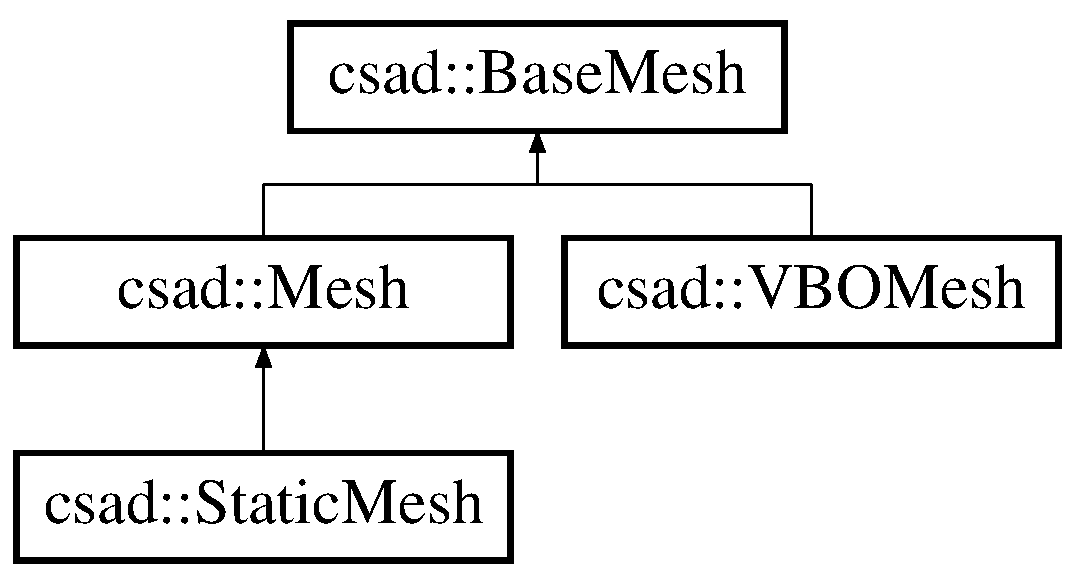
\includegraphics[height=3.000000cm]{classcsad_1_1_base_mesh}
\end{center}
\end{figure}


\subsection{Detailed Description}
\hyperlink{classcsad_1_1_base_mesh}{Base\-Mesh} -\/ abstract class geometry. 

\begin{DoxySeeAlso}{See Also}
\hyperlink{group__scene}{csad\-: scene} 
\end{DoxySeeAlso}

\hypertarget{classcsad_1_1_base_object}{\section{csad\-:\-:Base\-Object Class Reference}
\label{classcsad_1_1_base_object}\index{csad\-::\-Base\-Object@{csad\-::\-Base\-Object}}
}


\hyperlink{classcsad_1_1_base_object}{Base\-Object} -\/ the main interface objects.  


Inheritance diagram for csad\-:\-:Base\-Object\-:\begin{figure}[H]
\begin{center}
\leavevmode
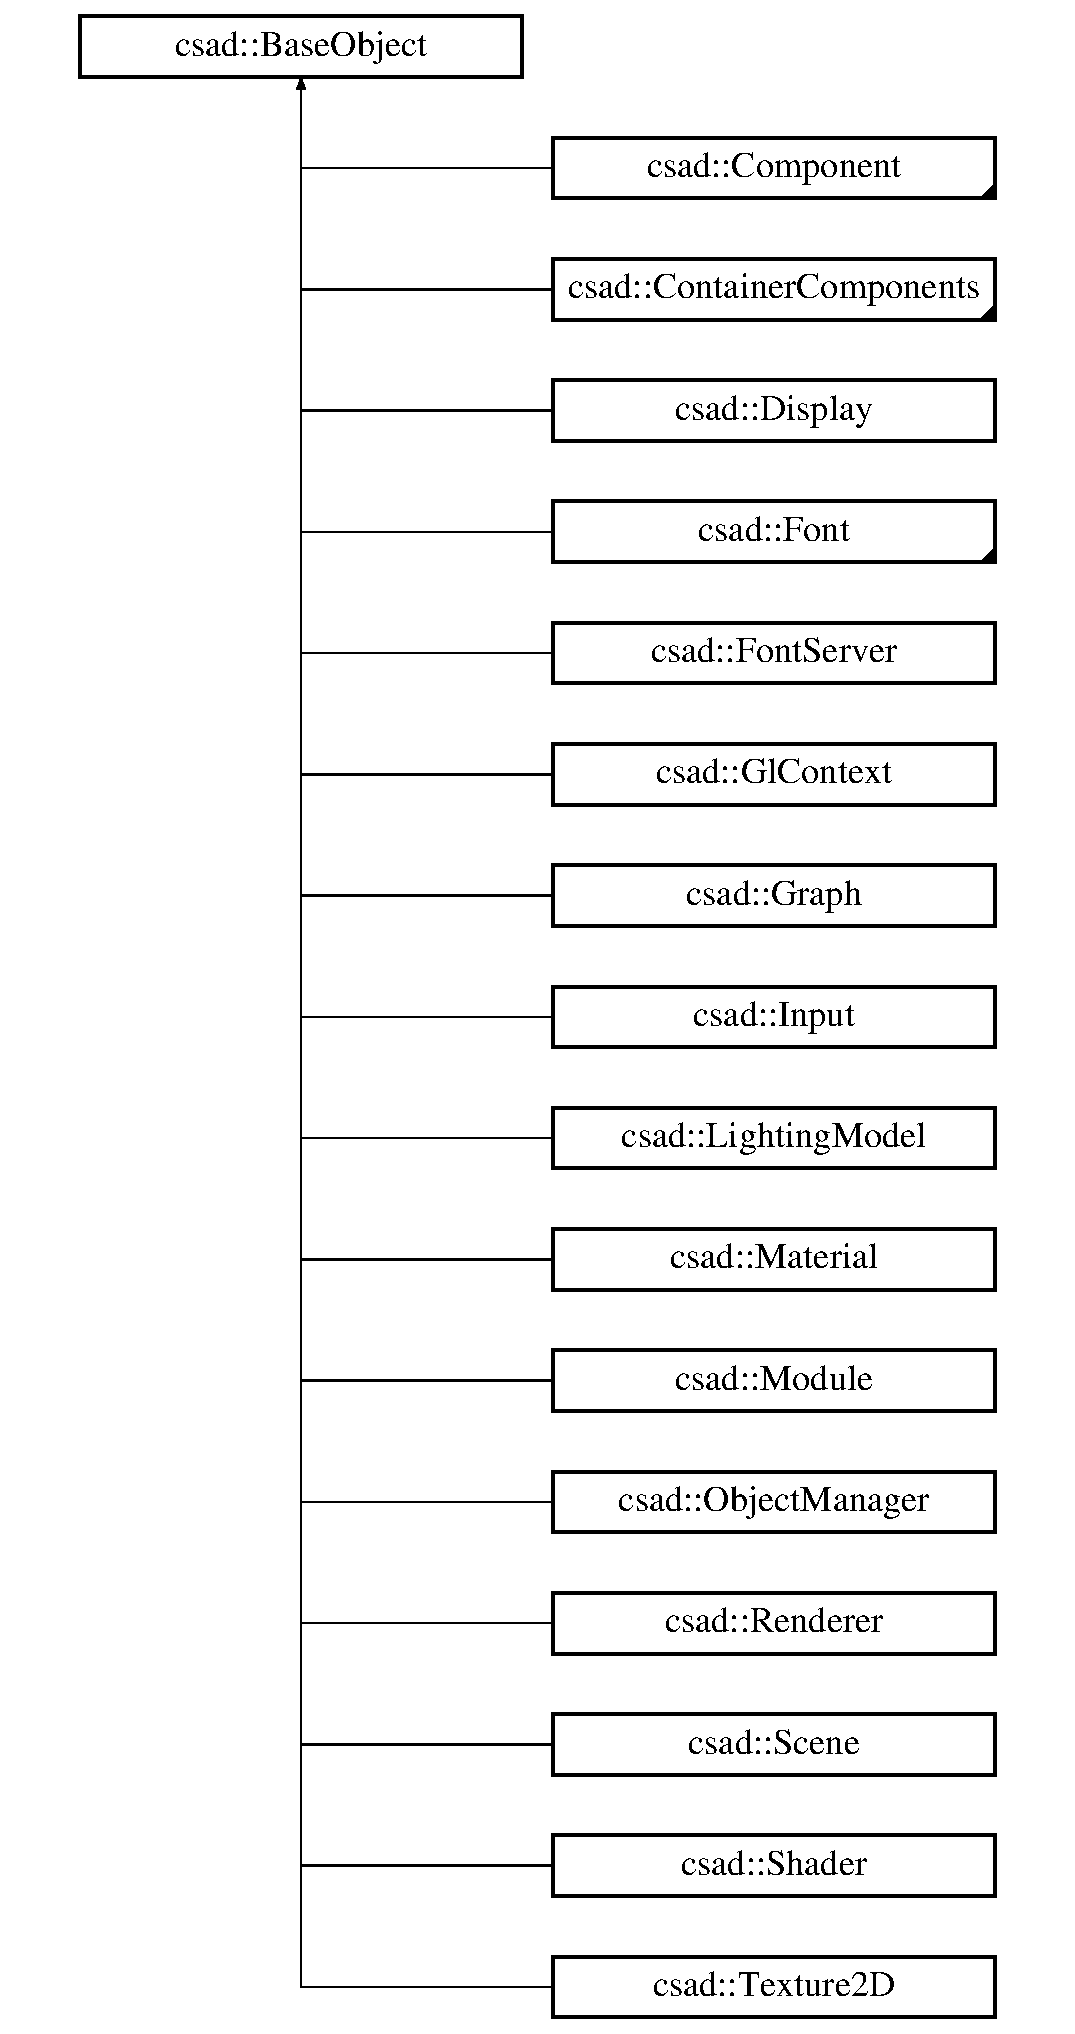
\includegraphics[height=12.000000cm]{classcsad_1_1_base_object}
\end{center}
\end{figure}
\subsection*{Public Types}
\begin{DoxyCompactItemize}
\item 
enum \hyperlink{classcsad_1_1_base_object_a27d9db492c1a385aa4086da1824e2737}{B\-A\-S\-E} \{ \\*
\hyperlink{classcsad_1_1_base_object_a27d9db492c1a385aa4086da1824e2737a9ab99f6059466c7ce51004dd5938d35c}{A\-N\-Y} = 0x00000000, 
\hyperlink{classcsad_1_1_base_object_a27d9db492c1a385aa4086da1824e2737ad2103561ac9ca4b765a4c36914a7df02}{E\-V\-E\-N\-T} = 0x00000001, 
\hyperlink{classcsad_1_1_base_object_a27d9db492c1a385aa4086da1824e2737a6e23bbf77d9292172cc59b14d1cb4d04}{T\-Y\-P\-E} = 0x00000002, 
\hyperlink{classcsad_1_1_base_object_a27d9db492c1a385aa4086da1824e2737a43ab8e97faa9873019a54520280f4eb2}{C\-O\-N\-T\-A\-I\-N\-E\-R} = 0x00000003, 
\\*
\hyperlink{classcsad_1_1_base_object_a27d9db492c1a385aa4086da1824e2737a4ba0c7bad15c4e5eca45fb0e5ce830ca}{M\-A\-N\-A\-G\-E\-R\-\_\-\-C\-O\-U\-N\-T} = 0x00000004, 
\hyperlink{classcsad_1_1_base_object_a27d9db492c1a385aa4086da1824e2737a540e44bba71ec276cec84723ce1f6523}{M\-A\-N\-A\-G\-E\-R} = 0x00000005, 
\hyperlink{classcsad_1_1_base_object_a27d9db492c1a385aa4086da1824e2737af9ddc40b2b5ec6bb34f770700291fc08}{W\-R\-I\-T\-E} = 0x00000006, 
\hyperlink{classcsad_1_1_base_object_a27d9db492c1a385aa4086da1824e2737ac59c8af3c3e1a023abfeb4bd3eff7aa2}{R\-E\-A\-D} = 0x00000007, 
\\*
\hyperlink{classcsad_1_1_base_object_a27d9db492c1a385aa4086da1824e2737a1ad754d1312e455b8585419a33bba1bf}{S\-E\-L\-E\-C\-T} = 0x00000008, 
\hyperlink{classcsad_1_1_base_object_a27d9db492c1a385aa4086da1824e2737a10c28c9ee2a345bcc225baa078bf4752}{R\-U\-N} = 0x00000009, 
\hyperlink{classcsad_1_1_base_object_a27d9db492c1a385aa4086da1824e2737a6c87574035e30093ab61437967c0d61f}{L\-I\-S\-T} = 0x0000000\-A, 
\hyperlink{classcsad_1_1_base_object_a27d9db492c1a385aa4086da1824e2737a0fc048a20a58fb4f821beecee64ff361}{L\-I\-S\-T\-\_\-\-C\-O\-U\-N\-T} = 0x0000000\-B, 
\\*
\hyperlink{classcsad_1_1_base_object_a27d9db492c1a385aa4086da1824e2737a8e31010e573395e2cd42ae65e2f30d61}{N\-A\-M\-E} = 0x0000000\-C, 
\hyperlink{classcsad_1_1_base_object_a27d9db492c1a385aa4086da1824e2737a58634a1a515a3896051bf0e99a763253}{C\-H\-I\-L\-D\-\_\-\-N\-A\-M\-E} = 0x0000000\-D
 \}
\begin{DoxyCompactList}\small\item\em the basic format of the interface \end{DoxyCompactList}\end{DoxyCompactItemize}
\subsection*{Public Member Functions}
\begin{DoxyCompactItemize}
\item 
\hypertarget{classcsad_1_1_base_object_ada59b9a0425d74cea61c1f277b580130}{\-\_\-\-F\-O\-R\-C\-E\-I\-N\-L\-I\-N\-E bool \hyperlink{classcsad_1_1_base_object_ada59b9a0425d74cea61c1f277b580130}{is\-Container} ()}\label{classcsad_1_1_base_object_ada59b9a0425d74cea61c1f277b580130}

\begin{DoxyCompactList}\small\item\em returns true if the object is a container. \end{DoxyCompactList}\item 
\hypertarget{classcsad_1_1_base_object_addc5ee69c7bb96a4a654cadecb3e547d}{\-\_\-\-F\-O\-R\-C\-E\-I\-N\-L\-I\-N\-E \hyperlink{classbt_1_1_parameters_list}{Parameters\-List} $\ast$ \hyperlink{classcsad_1_1_base_object_addc5ee69c7bb96a4a654cadecb3e547d}{read} (\hyperlink{classbt_1_1_parameters_list}{Parameters\-List} $\ast$data)}\label{classcsad_1_1_base_object_addc5ee69c7bb96a4a654cadecb3e547d}

\begin{DoxyCompactList}\small\item\em read attributes object. \end{DoxyCompactList}\item 
\hypertarget{classcsad_1_1_base_object_aa8d3a855874527b14a5c56f629789b1f}{virtual void $\ast$ \hyperlink{classcsad_1_1_base_object_aa8d3a855874527b14a5c56f629789b1f}{set} (unsigned \-\_\-int32, void $\ast$)=0}\label{classcsad_1_1_base_object_aa8d3a855874527b14a5c56f629789b1f}

\begin{DoxyCompactList}\small\item\em used for any interface commands. \end{DoxyCompactList}\item 
\hypertarget{classcsad_1_1_base_object_a6ae52b3ccd891d23b270fbb837322d1b}{\-\_\-\-F\-O\-R\-C\-E\-I\-N\-L\-I\-N\-E void $\ast$ \hyperlink{classcsad_1_1_base_object_a6ae52b3ccd891d23b270fbb837322d1b}{type} ()}\label{classcsad_1_1_base_object_a6ae52b3ccd891d23b270fbb837322d1b}

\begin{DoxyCompactList}\small\item\em the output pointer to the typeid() of the class. \end{DoxyCompactList}\item 
\hypertarget{classcsad_1_1_base_object_a588a28a35b2aefa0a833405f152d73e4}{\-\_\-\-F\-O\-R\-C\-E\-I\-N\-L\-I\-N\-E void \hyperlink{classcsad_1_1_base_object_a588a28a35b2aefa0a833405f152d73e4}{write} (\hyperlink{classbt_1_1_parameters_list}{Parameters\-List} $\ast$data)}\label{classcsad_1_1_base_object_a588a28a35b2aefa0a833405f152d73e4}

\begin{DoxyCompactList}\small\item\em record attributes of the object. \end{DoxyCompactList}\end{DoxyCompactItemize}


\subsection{Detailed Description}
\hyperlink{classcsad_1_1_base_object}{Base\-Object} -\/ the main interface objects. 

The basic template for description in the header\-: \begin{DoxyVerb}  class SomeClass:public csad::Component {
     public:
     ...
         void * set(unsinged _int32 id,void * params);

      TYPEINFO_H
     private:
     ...
  }
\end{DoxyVerb}


The basic template for describing the implementation\-: \begin{DoxyVerb}  void * SomeClass::set(unsinged _int32 id,void * params)
  {
     if (id==csad::BaseObject::TYPE) return SomeClassL::t();
     return 0;
  }

  TYPEINFO(SomeClass);
\end{DoxyVerb}


\begin{DoxySeeAlso}{See Also}
\hyperlink{group__core}{csad\-: core} 
\end{DoxySeeAlso}


\subsection{Member Enumeration Documentation}
\hypertarget{classcsad_1_1_base_object_a27d9db492c1a385aa4086da1824e2737}{\index{csad\-::\-Base\-Object@{csad\-::\-Base\-Object}!B\-A\-S\-E@{B\-A\-S\-E}}
\index{B\-A\-S\-E@{B\-A\-S\-E}!csad::BaseObject@{csad\-::\-Base\-Object}}
\subsubsection[{B\-A\-S\-E}]{\setlength{\rightskip}{0pt plus 5cm}enum {\bf csad\-::\-Base\-Object\-::\-B\-A\-S\-E}}}\label{classcsad_1_1_base_object_a27d9db492c1a385aa4086da1824e2737}


the basic format of the interface 

\begin{Desc}
\item[Enumerator]\par
\begin{description}
\index{A\-N\-Y@{A\-N\-Y}!csad\-::\-Base\-Object@{csad\-::\-Base\-Object}}\index{csad\-::\-Base\-Object@{csad\-::\-Base\-Object}!A\-N\-Y@{A\-N\-Y}}\item[{\em 
\hypertarget{classcsad_1_1_base_object_a27d9db492c1a385aa4086da1824e2737a9ab99f6059466c7ce51004dd5938d35c}{A\-N\-Y}\label{classcsad_1_1_base_object_a27d9db492c1a385aa4086da1824e2737a9ab99f6059466c7ce51004dd5938d35c}
}]specific identifier \index{E\-V\-E\-N\-T@{E\-V\-E\-N\-T}!csad\-::\-Base\-Object@{csad\-::\-Base\-Object}}\index{csad\-::\-Base\-Object@{csad\-::\-Base\-Object}!E\-V\-E\-N\-T@{E\-V\-E\-N\-T}}\item[{\em 
\hypertarget{classcsad_1_1_base_object_a27d9db492c1a385aa4086da1824e2737ad2103561ac9ca4b765a4c36914a7df02}{E\-V\-E\-N\-T}\label{classcsad_1_1_base_object_a27d9db492c1a385aa4086da1824e2737ad2103561ac9ca4b765a4c36914a7df02}
}]processing messages \index{T\-Y\-P\-E@{T\-Y\-P\-E}!csad\-::\-Base\-Object@{csad\-::\-Base\-Object}}\index{csad\-::\-Base\-Object@{csad\-::\-Base\-Object}!T\-Y\-P\-E@{T\-Y\-P\-E}}\item[{\em 
\hypertarget{classcsad_1_1_base_object_a27d9db492c1a385aa4086da1824e2737a6e23bbf77d9292172cc59b14d1cb4d04}{T\-Y\-P\-E}\label{classcsad_1_1_base_object_a27d9db492c1a385aa4086da1824e2737a6e23bbf77d9292172cc59b14d1cb4d04}
}]the output pointer to the typeid() of the class; \index{C\-O\-N\-T\-A\-I\-N\-E\-R@{C\-O\-N\-T\-A\-I\-N\-E\-R}!csad\-::\-Base\-Object@{csad\-::\-Base\-Object}}\index{csad\-::\-Base\-Object@{csad\-::\-Base\-Object}!C\-O\-N\-T\-A\-I\-N\-E\-R@{C\-O\-N\-T\-A\-I\-N\-E\-R}}\item[{\em 
\hypertarget{classcsad_1_1_base_object_a27d9db492c1a385aa4086da1824e2737a43ab8e97faa9873019a54520280f4eb2}{C\-O\-N\-T\-A\-I\-N\-E\-R}\label{classcsad_1_1_base_object_a27d9db492c1a385aa4086da1824e2737a43ab8e97faa9873019a54520280f4eb2}
}]returns a pointer to itself if the object is a container. \index{M\-A\-N\-A\-G\-E\-R\-\_\-\-C\-O\-U\-N\-T@{M\-A\-N\-A\-G\-E\-R\-\_\-\-C\-O\-U\-N\-T}!csad\-::\-Base\-Object@{csad\-::\-Base\-Object}}\index{csad\-::\-Base\-Object@{csad\-::\-Base\-Object}!M\-A\-N\-A\-G\-E\-R\-\_\-\-C\-O\-U\-N\-T@{M\-A\-N\-A\-G\-E\-R\-\_\-\-C\-O\-U\-N\-T}}\item[{\em 
\hypertarget{classcsad_1_1_base_object_a27d9db492c1a385aa4086da1824e2737a4ba0c7bad15c4e5eca45fb0e5ce830ca}{M\-A\-N\-A\-G\-E\-R\-\_\-\-C\-O\-U\-N\-T}\label{classcsad_1_1_base_object_a27d9db492c1a385aa4086da1824e2737a4ba0c7bad15c4e5eca45fb0e5ce830ca}
}]returns the number of managers. \index{M\-A\-N\-A\-G\-E\-R@{M\-A\-N\-A\-G\-E\-R}!csad\-::\-Base\-Object@{csad\-::\-Base\-Object}}\index{csad\-::\-Base\-Object@{csad\-::\-Base\-Object}!M\-A\-N\-A\-G\-E\-R@{M\-A\-N\-A\-G\-E\-R}}\item[{\em 
\hypertarget{classcsad_1_1_base_object_a27d9db492c1a385aa4086da1824e2737a540e44bba71ec276cec84723ce1f6523}{M\-A\-N\-A\-G\-E\-R}\label{classcsad_1_1_base_object_a27d9db492c1a385aa4086da1824e2737a540e44bba71ec276cec84723ce1f6523}
}]returns the specified Manager \index{W\-R\-I\-T\-E@{W\-R\-I\-T\-E}!csad\-::\-Base\-Object@{csad\-::\-Base\-Object}}\index{csad\-::\-Base\-Object@{csad\-::\-Base\-Object}!W\-R\-I\-T\-E@{W\-R\-I\-T\-E}}\item[{\em 
\hypertarget{classcsad_1_1_base_object_a27d9db492c1a385aa4086da1824e2737af9ddc40b2b5ec6bb34f770700291fc08}{W\-R\-I\-T\-E}\label{classcsad_1_1_base_object_a27d9db492c1a385aa4086da1824e2737af9ddc40b2b5ec6bb34f770700291fc08}
}]record attributes of the object, the input is the list of parameters Object\-Parameters \index{R\-E\-A\-D@{R\-E\-A\-D}!csad\-::\-Base\-Object@{csad\-::\-Base\-Object}}\index{csad\-::\-Base\-Object@{csad\-::\-Base\-Object}!R\-E\-A\-D@{R\-E\-A\-D}}\item[{\em 
\hypertarget{classcsad_1_1_base_object_a27d9db492c1a385aa4086da1824e2737ac59c8af3c3e1a023abfeb4bd3eff7aa2}{R\-E\-A\-D}\label{classcsad_1_1_base_object_a27d9db492c1a385aa4086da1824e2737ac59c8af3c3e1a023abfeb4bd3eff7aa2}
}]read attributes object, the input is empty list of parameters Object\-Parameters filled and fed to the output \index{S\-E\-L\-E\-C\-T@{S\-E\-L\-E\-C\-T}!csad\-::\-Base\-Object@{csad\-::\-Base\-Object}}\index{csad\-::\-Base\-Object@{csad\-::\-Base\-Object}!S\-E\-L\-E\-C\-T@{S\-E\-L\-E\-C\-T}}\item[{\em 
\hypertarget{classcsad_1_1_base_object_a27d9db492c1a385aa4086da1824e2737a1ad754d1312e455b8585419a33bba1bf}{S\-E\-L\-E\-C\-T}\label{classcsad_1_1_base_object_a27d9db492c1a385aa4086da1824e2737a1ad754d1312e455b8585419a33bba1bf}
}]selection event has its peculiarities \index{R\-U\-N@{R\-U\-N}!csad\-::\-Base\-Object@{csad\-::\-Base\-Object}}\index{csad\-::\-Base\-Object@{csad\-::\-Base\-Object}!R\-U\-N@{R\-U\-N}}\item[{\em 
\hypertarget{classcsad_1_1_base_object_a27d9db492c1a385aa4086da1824e2737a10c28c9ee2a345bcc225baa078bf4752}{R\-U\-N}\label{classcsad_1_1_base_object_a27d9db492c1a385aa4086da1824e2737a10c28c9ee2a345bcc225baa078bf4752}
}]to execute the method \index{L\-I\-S\-T@{L\-I\-S\-T}!csad\-::\-Base\-Object@{csad\-::\-Base\-Object}}\index{csad\-::\-Base\-Object@{csad\-::\-Base\-Object}!L\-I\-S\-T@{L\-I\-S\-T}}\item[{\em 
\hypertarget{classcsad_1_1_base_object_a27d9db492c1a385aa4086da1824e2737a6c87574035e30093ab61437967c0d61f}{L\-I\-S\-T}\label{classcsad_1_1_base_object_a27d9db492c1a385aa4086da1824e2737a6c87574035e30093ab61437967c0d61f}
}]returns the list item \index{L\-I\-S\-T\-\_\-\-C\-O\-U\-N\-T@{L\-I\-S\-T\-\_\-\-C\-O\-U\-N\-T}!csad\-::\-Base\-Object@{csad\-::\-Base\-Object}}\index{csad\-::\-Base\-Object@{csad\-::\-Base\-Object}!L\-I\-S\-T\-\_\-\-C\-O\-U\-N\-T@{L\-I\-S\-T\-\_\-\-C\-O\-U\-N\-T}}\item[{\em 
\hypertarget{classcsad_1_1_base_object_a27d9db492c1a385aa4086da1824e2737a0fc048a20a58fb4f821beecee64ff361}{L\-I\-S\-T\-\_\-\-C\-O\-U\-N\-T}\label{classcsad_1_1_base_object_a27d9db492c1a385aa4086da1824e2737a0fc048a20a58fb4f821beecee64ff361}
}]number of items \index{N\-A\-M\-E@{N\-A\-M\-E}!csad\-::\-Base\-Object@{csad\-::\-Base\-Object}}\index{csad\-::\-Base\-Object@{csad\-::\-Base\-Object}!N\-A\-M\-E@{N\-A\-M\-E}}\item[{\em 
\hypertarget{classcsad_1_1_base_object_a27d9db492c1a385aa4086da1824e2737a8e31010e573395e2cd42ae65e2f30d61}{N\-A\-M\-E}\label{classcsad_1_1_base_object_a27d9db492c1a385aa4086da1824e2737a8e31010e573395e2cd42ae65e2f30d61}
}]returns the name if it is. \index{C\-H\-I\-L\-D\-\_\-\-N\-A\-M\-E@{C\-H\-I\-L\-D\-\_\-\-N\-A\-M\-E}!csad\-::\-Base\-Object@{csad\-::\-Base\-Object}}\index{csad\-::\-Base\-Object@{csad\-::\-Base\-Object}!C\-H\-I\-L\-D\-\_\-\-N\-A\-M\-E@{C\-H\-I\-L\-D\-\_\-\-N\-A\-M\-E}}\item[{\em 
\hypertarget{classcsad_1_1_base_object_a27d9db492c1a385aa4086da1824e2737a58634a1a515a3896051bf0e99a763253}{C\-H\-I\-L\-D\-\_\-\-N\-A\-M\-E}\label{classcsad_1_1_base_object_a27d9db492c1a385aa4086da1824e2737a58634a1a515a3896051bf0e99a763253}
}]returns the name if it is. \end{description}
\end{Desc}

\hypertarget{classcsad_1_1_camera}{\section{csad\-:\-:Camera Class Reference}
\label{classcsad_1_1_camera}\index{csad\-::\-Camera@{csad\-::\-Camera}}
}


\hyperlink{classcsad_1_1_camera}{Camera} -\/ component defines the projection matrix of points \hyperlink{classcsad_1_1_transform}{Transform} into a point Target.  


Inheritance diagram for csad\-:\-:Camera\-:\begin{figure}[H]
\begin{center}
\leavevmode
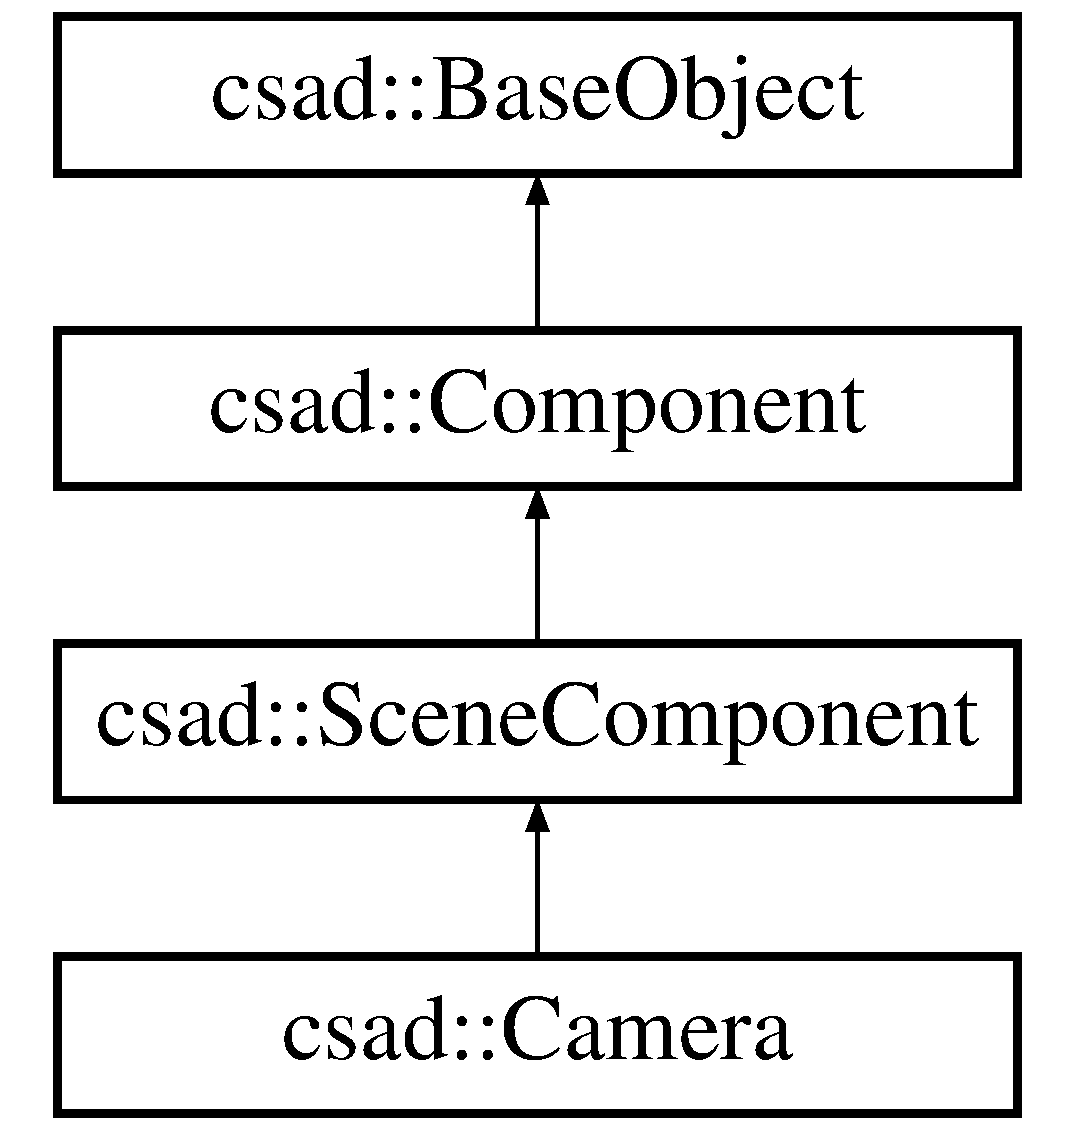
\includegraphics[height=4.000000cm]{classcsad_1_1_camera}
\end{center}
\end{figure}
\subsection*{Public Member Functions}
\begin{DoxyCompactItemize}
\item 
\hypertarget{classcsad_1_1_camera_ad2e3a823499909d9d4970aad87f06221}{\-\_\-\-F\-O\-R\-C\-E\-I\-N\-L\-I\-N\-E bool \hyperlink{classcsad_1_1_camera_ad2e3a823499909d9d4970aad87f06221}{clear\-Color} ()}\label{classcsad_1_1_camera_ad2e3a823499909d9d4970aad87f06221}

\begin{DoxyCompactList}\small\item\em Return true if color frame have the background. \end{DoxyCompactList}\item 
\hypertarget{classcsad_1_1_camera_a8d663d371fc45973754cd34298021260}{\-\_\-\-F\-O\-R\-C\-E\-I\-N\-L\-I\-N\-E bool \hyperlink{classcsad_1_1_camera_a8d663d371fc45973754cd34298021260}{clear\-Depth} ()}\label{classcsad_1_1_camera_a8d663d371fc45973754cd34298021260}

\begin{DoxyCompactList}\small\item\em Return true if depth frame cleanning before render. \end{DoxyCompactList}\item 
\hypertarget{classcsad_1_1_camera_af2885672eda9f42ed2fd0057fc0b692a}{\-\_\-\-F\-O\-R\-C\-E\-I\-N\-L\-I\-N\-E bool \hyperlink{classcsad_1_1_camera_af2885672eda9f42ed2fd0057fc0b692a}{cull\-Face} ()}\label{classcsad_1_1_camera_af2885672eda9f42ed2fd0057fc0b692a}

\begin{DoxyCompactList}\small\item\em return state \end{DoxyCompactList}\item 
\hypertarget{classcsad_1_1_camera_a78f6b71f2fddeb774cb22c361b03fc97}{\-\_\-\-F\-O\-R\-C\-E\-I\-N\-L\-I\-N\-E bool \hyperlink{classcsad_1_1_camera_a78f6b71f2fddeb774cb22c361b03fc97}{front\-Face} ()}\label{classcsad_1_1_camera_a78f6b71f2fddeb774cb22c361b03fc97}

\begin{DoxyCompactList}\small\item\em return state \end{DoxyCompactList}\item 
\hypertarget{classcsad_1_1_camera_ace0dd65d8658ff3dc1dd37602243c71a}{\-\_\-\-F\-O\-R\-C\-E\-I\-N\-L\-I\-N\-E double \hyperlink{classcsad_1_1_camera_ace0dd65d8658ff3dc1dd37602243c71a}{get\-Fov} ()}\label{classcsad_1_1_camera_ace0dd65d8658ff3dc1dd37602243c71a}

\begin{DoxyCompactList}\small\item\em Return the angle of view or the frame size. \end{DoxyCompactList}\item 
\hypertarget{classcsad_1_1_camera_a88294fd2c5d1fa031f2bb3b8313324f3}{\-\_\-\-F\-O\-R\-C\-E\-I\-N\-L\-I\-N\-E double \hyperlink{classcsad_1_1_camera_a88294fd2c5d1fa031f2bb3b8313324f3}{get\-Max\-Range} ()}\label{classcsad_1_1_camera_a88294fd2c5d1fa031f2bb3b8313324f3}

\begin{DoxyCompactList}\small\item\em Return distance of far clipping plane. \end{DoxyCompactList}\item 
\hypertarget{classcsad_1_1_camera_a3c0b05f05093921f11ac61d03aa6ec3d}{\-\_\-\-F\-O\-R\-C\-E\-I\-N\-L\-I\-N\-E double \hyperlink{classcsad_1_1_camera_a3c0b05f05093921f11ac61d03aa6ec3d}{get\-Min\-Range} ()}\label{classcsad_1_1_camera_a3c0b05f05093921f11ac61d03aa6ec3d}

\begin{DoxyCompactList}\small\item\em Return distance of near clipping plane. \end{DoxyCompactList}\item 
\hypertarget{classcsad_1_1_camera_a02bda0f3de8b0bff0832e1497d4da9c4}{\-\_\-\-F\-O\-R\-C\-E\-I\-N\-L\-I\-N\-E unsigned int \hyperlink{classcsad_1_1_camera_a02bda0f3de8b0bff0832e1497d4da9c4}{get\-Proj} ()}\label{classcsad_1_1_camera_a02bda0f3de8b0bff0832e1497d4da9c4}

\begin{DoxyCompactList}\small\item\em Return model projection. \end{DoxyCompactList}\item 
\hypertarget{classcsad_1_1_camera_a46822b3370620e607b16fdc90464cb28}{C\-S\-A\-D\-\_\-\-A\-P\-I \hyperlink{classcsad_1_1_scene}{Scene} $\ast$ \hyperlink{classcsad_1_1_camera_a46822b3370620e607b16fdc90464cb28}{get\-Scene} ()}\label{classcsad_1_1_camera_a46822b3370620e607b16fdc90464cb28}

\begin{DoxyCompactList}\small\item\em The environment belongs to the camera. \end{DoxyCompactList}\item 
\hypertarget{classcsad_1_1_camera_a84500df7c9acb978dd957fdb69cc481f}{C\-S\-A\-D\-\_\-\-A\-P\-I \hyperlink{classbt_1_1vector4f}{vector4f} \hyperlink{classcsad_1_1_camera_a84500df7c9acb978dd957fdb69cc481f}{get\-View\-Port} ()}\label{classcsad_1_1_camera_a84500df7c9acb978dd957fdb69cc481f}

\begin{DoxyCompactList}\small\item\em Returns the position and dimensions of the window display, in percent. \end{DoxyCompactList}\item 
\hypertarget{classcsad_1_1_camera_aa99f6cef6f085590aede1b6f158db1d7}{C\-S\-A\-D\-\_\-\-A\-P\-I \hyperlink{classbt_1_1vector4i}{vector4i} \hyperlink{classcsad_1_1_camera_aa99f6cef6f085590aede1b6f158db1d7}{get\-View\-Port} (\hyperlink{classcsad_1_1_gl_context}{Gl\-Context} $\ast$context)}\label{classcsad_1_1_camera_aa99f6cef6f085590aede1b6f158db1d7}

\begin{DoxyCompactList}\small\item\em Returns the position and dimensions of the display window, in pixels. \end{DoxyCompactList}\item 
\hypertarget{classcsad_1_1_camera_a8bc7d426bf9cd731d6bd0818082dde34}{C\-S\-A\-D\-\_\-\-A\-P\-I \hyperlink{classbt_1_1vector4i}{vector4i} \hyperlink{classcsad_1_1_camera_a8bc7d426bf9cd731d6bd0818082dde34}{get\-View\-Port} (\hyperlink{classcsad_1_1_display}{Display} $\ast$display)}\label{classcsad_1_1_camera_a8bc7d426bf9cd731d6bd0818082dde34}

\begin{DoxyCompactList}\small\item\em Returns the position and dimensions of the display window, in pixels. \end{DoxyCompactList}\item 
\hypertarget{classcsad_1_1_camera_ae48f1f5d3baaacf1a1b793e45c2389c1}{C\-S\-A\-D\-\_\-\-A\-P\-I bool \hyperlink{classcsad_1_1_camera_ae48f1f5d3baaacf1a1b793e45c2389c1}{make\-Current} (unsigned int to\-Texture\-Id=0)}\label{classcsad_1_1_camera_ae48f1f5d3baaacf1a1b793e45c2389c1}

\begin{DoxyCompactList}\small\item\em Setting projection matrix. \end{DoxyCompactList}\item 
\hypertarget{classcsad_1_1_camera_a59dd6f411c4fd88191751842cc963f9d}{C\-S\-A\-D\-\_\-\-A\-P\-I bool \hyperlink{classcsad_1_1_camera_a59dd6f411c4fd88191751842cc963f9d}{make\-Current} (\hyperlink{classbt_1_1vector4i}{vector4i} \&rect, unsigned int to\-Texture\-Id=0)}\label{classcsad_1_1_camera_a59dd6f411c4fd88191751842cc963f9d}

\begin{DoxyCompactList}\small\item\em Setting projection matrices, and the region's display. \end{DoxyCompactList}\item 
\hypertarget{classcsad_1_1_camera_a0e4c86b157f37298499a7af6d9ae9cd9}{C\-S\-A\-D\-\_\-\-A\-P\-I \hyperlink{classbt_1_1matrix4f}{matrix4f} $\ast$ \hyperlink{classcsad_1_1_camera_a0e4c86b157f37298499a7af6d9ae9cd9}{proj\-Matrix} ()}\label{classcsad_1_1_camera_a0e4c86b157f37298499a7af6d9ae9cd9}

\begin{DoxyCompactList}\small\item\em returns the projection matrix. \end{DoxyCompactList}\item 
\hypertarget{classcsad_1_1_camera_a0ca732a715c6dac01e00620123327409}{C\-S\-A\-D\-\_\-\-A\-P\-I void $\ast$ \hyperlink{classcsad_1_1_camera_a0ca732a715c6dac01e00620123327409}{set} (unsigned \-\_\-int32, void $\ast$)}\label{classcsad_1_1_camera_a0ca732a715c6dac01e00620123327409}

\begin{DoxyCompactList}\small\item\em used for any interface commands. \end{DoxyCompactList}\item 
\hypertarget{classcsad_1_1_camera_af5c035da21ccd3604305ecf1539a434e}{\-\_\-\-F\-O\-R\-C\-E\-I\-N\-L\-I\-N\-E void \hyperlink{classcsad_1_1_camera_af5c035da21ccd3604305ecf1539a434e}{set\-Clear\-Color} (bool is)}\label{classcsad_1_1_camera_af5c035da21ccd3604305ecf1539a434e}

\begin{DoxyCompactList}\small\item\em Specifies whether frame to have the background, the performance is better off. \end{DoxyCompactList}\item 
\hypertarget{classcsad_1_1_camera_aa8c89f2ac7bfbb0e2f5380bd58fa74b8}{C\-S\-A\-D\-\_\-\-A\-P\-I \hyperlink{classcsad_1_1_camera}{Camera} \& \hyperlink{classcsad_1_1_camera_aa8c89f2ac7bfbb0e2f5380bd58fa74b8}{set\-Color} (float r, float g, float b, float w)}\label{classcsad_1_1_camera_aa8c89f2ac7bfbb0e2f5380bd58fa74b8}

\begin{DoxyCompactList}\small\item\em Sets the color of the background, automatically includes the background. \end{DoxyCompactList}\item 
\hypertarget{classcsad_1_1_camera_a7e212777db0eba5791e9bdc17a9f1e1c}{C\-S\-A\-D\-\_\-\-A\-P\-I \hyperlink{classcsad_1_1_camera}{Camera} \& \hyperlink{classcsad_1_1_camera_a7e212777db0eba5791e9bdc17a9f1e1c}{set\-Color} (\hyperlink{classbt_1_1vector4f}{vector4f} \&color)}\label{classcsad_1_1_camera_a7e212777db0eba5791e9bdc17a9f1e1c}

\begin{DoxyCompactList}\small\item\em Sets the color of the background, automatically includes the background. \end{DoxyCompactList}\item 
\hypertarget{classcsad_1_1_camera_ad56a98a01c19be324ed7e9f6dc94b88c}{\-\_\-\-F\-O\-R\-C\-E\-I\-N\-L\-I\-N\-E void \hyperlink{classcsad_1_1_camera_ad56a98a01c19be324ed7e9f6dc94b88c}{set\-Cull\-Face} (bool is)}\label{classcsad_1_1_camera_ad56a98a01c19be324ed7e9f6dc94b88c}

\begin{DoxyCompactList}\small\item\em set true if need back of front face hide \end{DoxyCompactList}\item 
\hypertarget{classcsad_1_1_camera_a59f0490c8eef4fe181ecdb19f59640bb}{C\-S\-A\-D\-\_\-\-A\-P\-I \hyperlink{classcsad_1_1_camera}{Camera} \& \hyperlink{classcsad_1_1_camera_a59f0490c8eef4fe181ecdb19f59640bb}{set\-Depth} (double val)}\label{classcsad_1_1_camera_a59f0490c8eef4fe181ecdb19f59640bb}

\begin{DoxyCompactList}\small\item\em Sets the value of the depth. \end{DoxyCompactList}\item 
\hypertarget{classcsad_1_1_camera_a06aab87cdd1c891cf02918adcff10d96}{C\-S\-A\-D\-\_\-\-A\-P\-I \hyperlink{classcsad_1_1_camera}{Camera} \& \hyperlink{classcsad_1_1_camera_a06aab87cdd1c891cf02918adcff10d96}{set\-Fov} (double \-\_\-ov)}\label{classcsad_1_1_camera_a06aab87cdd1c891cf02918adcff10d96}

\begin{DoxyCompactList}\small\item\em Depending on the model projection sets the angle of view or the frame size. \end{DoxyCompactList}\item 
\hypertarget{classcsad_1_1_camera_aa65e2c0df44a14cc545fedfbd010baba}{\-\_\-\-F\-O\-R\-C\-E\-I\-N\-L\-I\-N\-E void \hyperlink{classcsad_1_1_camera_aa65e2c0df44a14cc545fedfbd010baba}{set\-Front\-Face} (bool is)}\label{classcsad_1_1_camera_aa65e2c0df44a14cc545fedfbd010baba}

\begin{DoxyCompactList}\small\item\em set true if need front face show \end{DoxyCompactList}\item 
\hypertarget{classcsad_1_1_camera_a493003b12fbba2386cba0a98ee827a40}{C\-S\-A\-D\-\_\-\-A\-P\-I \hyperlink{classcsad_1_1_camera}{Camera} \& \hyperlink{classcsad_1_1_camera_a493003b12fbba2386cba0a98ee827a40}{set\-Max\-Range} (double max)}\label{classcsad_1_1_camera_a493003b12fbba2386cba0a98ee827a40}

\begin{DoxyCompactList}\small\item\em Specifies the far clipping plane. \end{DoxyCompactList}\item 
\hypertarget{classcsad_1_1_camera_a2c8267221b07ae03a670c69121ca090c}{C\-S\-A\-D\-\_\-\-A\-P\-I \hyperlink{classcsad_1_1_camera}{Camera} \& \hyperlink{classcsad_1_1_camera_a2c8267221b07ae03a670c69121ca090c}{set\-Min\-Range} (double min)}\label{classcsad_1_1_camera_a2c8267221b07ae03a670c69121ca090c}

\begin{DoxyCompactList}\small\item\em Specifies near clipping. \end{DoxyCompactList}\item 
\hypertarget{classcsad_1_1_camera_ab2ea58997abbbd2b394397227c101595}{C\-S\-A\-D\-\_\-\-A\-P\-I \hyperlink{classcsad_1_1_camera}{Camera} \& \hyperlink{classcsad_1_1_camera_ab2ea58997abbbd2b394397227c101595}{set\-Proj} (unsigned int proj)}\label{classcsad_1_1_camera_ab2ea58997abbbd2b394397227c101595}

\begin{DoxyCompactList}\small\item\em Sets the model projection of this promising (Camera\-::\-Perspective) or orthogonal (Camera\-::\-Ortographic) \end{DoxyCompactList}\item 
\hypertarget{classcsad_1_1_camera_aa5f97dd128f03939dfe3f57ced8bd749}{C\-S\-A\-D\-\_\-\-A\-P\-I \hyperlink{classcsad_1_1_camera}{Camera} \& \hyperlink{classcsad_1_1_camera_aa5f97dd128f03939dfe3f57ced8bd749}{set\-View\-Port} (\hyperlink{classbt_1_1vector4f}{vector4f} $\ast$viewport)}\label{classcsad_1_1_camera_aa5f97dd128f03939dfe3f57ced8bd749}

\begin{DoxyCompactList}\small\item\em Sets the aspect ratio and position of the window in\% from the actual size of the context. \end{DoxyCompactList}\end{DoxyCompactItemize}
\subsection*{Static Public Member Functions}
\begin{DoxyCompactItemize}
\item 
\hypertarget{classcsad_1_1_camera_ae5b4cbfae3b97dd1aa3ba315c5a13f2a}{static C\-S\-A\-D\-\_\-\-A\-P\-I \hyperlink{classcsad_1_1_camera}{Camera} $\ast$ \hyperlink{classcsad_1_1_camera_ae5b4cbfae3b97dd1aa3ba315c5a13f2a}{finder} (char $\ast$path)}\label{classcsad_1_1_camera_ae5b4cbfae3b97dd1aa3ba315c5a13f2a}

\begin{DoxyCompactList}\small\item\em returns the camera in the specified path. \end{DoxyCompactList}\end{DoxyCompactItemize}
\subsection*{Additional Inherited Members}


\subsection{Detailed Description}
\hyperlink{classcsad_1_1_camera}{Camera} -\/ component defines the projection matrix of points \hyperlink{classcsad_1_1_transform}{Transform} into a point Target. 

For description in the configuration\-: \begin{DoxyVerb}  <Transform name="the name of the scene">
      <Camera fov="45" min="near plane" max="far plane" color="back color clean" depth="value for clean" cullface="" viewport="view rect"/>
  </Transform>
\end{DoxyVerb}


\begin{DoxySeeAlso}{See Also}
\hyperlink{classcsad_1_1_transform}{Transform}, \hyperlink{group__scene}{csad\-: scene} 
\end{DoxySeeAlso}

\hypertarget{classcsad_1_1_class_manager}{\section{csad\-:\-:Class\-Manager Class Reference}
\label{classcsad_1_1_class_manager}\index{csad\-::\-Class\-Manager@{csad\-::\-Class\-Manager}}
}


\hyperlink{classcsad_1_1_class_manager}{Class\-Manager} -\/ the Manager interface classes.  


\subsection*{Public Member Functions}
\begin{DoxyCompactItemize}
\item 
\hypertarget{classcsad_1_1_class_manager_a1b672a9bc1ce34daf388e278e4a877a0}{virtual void \hyperlink{classcsad_1_1_class_manager_a1b672a9bc1ce34daf388e278e4a877a0}{add\-Const} (const char $\ast$name, int c)=0}\label{classcsad_1_1_class_manager_a1b672a9bc1ce34daf388e278e4a877a0}

\begin{DoxyCompactList}\small\item\em Assigns the name of the constant value. \end{DoxyCompactList}\item 
\hypertarget{classcsad_1_1_class_manager_a60cb905c7bb8ffa55d7bdffcc6cf2bb1}{virtual const char $\ast$ \hyperlink{classcsad_1_1_class_manager_a60cb905c7bb8ffa55d7bdffcc6cf2bb1}{class\-Name} (void $\ast$type)=0}\label{classcsad_1_1_class_manager_a60cb905c7bb8ffa55d7bdffcc6cf2bb1}

\begin{DoxyCompactList}\small\item\em Returns the name of the specified type. \end{DoxyCompactList}\item 
\hypertarget{classcsad_1_1_class_manager_a7d52ba64630bd18ddecc08779c0a9d32}{virtual \hyperlink{classcsad_1_1_base_object}{Base\-Object} $\ast$ \hyperlink{classcsad_1_1_class_manager_a7d52ba64630bd18ddecc08779c0a9d32}{create\-Object} (char $\ast$\hyperlink{classcsad_1_1_class_manager_a60cb905c7bb8ffa55d7bdffcc6cf2bb1}{class\-Name}, \hyperlink{classbt_1_1_parameters_list}{Parameters\-List} $\ast$list)=0}\label{classcsad_1_1_class_manager_a7d52ba64630bd18ddecc08779c0a9d32}

\begin{DoxyCompactList}\small\item\em Creates object of the specified class and passes the parameter list. \end{DoxyCompactList}\item 
\hypertarget{classcsad_1_1_class_manager_ae20b1020a033cca51cd5c65b9af65709}{\-\_\-\-F\-O\-R\-C\-E\-I\-N\-L\-I\-N\-E \hyperlink{classcsad_1_1_base_object}{Base\-Object} $\ast$ \hyperlink{classcsad_1_1_class_manager_ae20b1020a033cca51cd5c65b9af65709}{create\-Object} (const char $\ast$\hyperlink{classcsad_1_1_class_manager_a60cb905c7bb8ffa55d7bdffcc6cf2bb1}{class\-Name}, \hyperlink{classbt_1_1_parameters_list}{Parameters\-List} $\ast$list)}\label{classcsad_1_1_class_manager_ae20b1020a033cca51cd5c65b9af65709}

\begin{DoxyCompactList}\small\item\em Creates object of the specified class and passes the parameter list. \end{DoxyCompactList}\item 
\hypertarget{classcsad_1_1_class_manager_a19ed7fb2c1775b5b5b69c65d4ad98a30}{virtual int \hyperlink{classcsad_1_1_class_manager_a19ed7fb2c1775b5b5b69c65d4ad98a30}{get\-Const} (char $\ast$name)=0}\label{classcsad_1_1_class_manager_a19ed7fb2c1775b5b5b69c65d4ad98a30}

\begin{DoxyCompactList}\small\item\em Returns a constant value of its name. \end{DoxyCompactList}\item 
\hypertarget{classcsad_1_1_class_manager_a99c542560743638f818f8cf3298fa51c}{\-\_\-\-F\-O\-R\-C\-E\-I\-N\-L\-I\-N\-E int \hyperlink{classcsad_1_1_class_manager_a99c542560743638f818f8cf3298fa51c}{get\-Const} (const char $\ast$name)}\label{classcsad_1_1_class_manager_a99c542560743638f818f8cf3298fa51c}

\begin{DoxyCompactList}\small\item\em Returns a constant value of its name. \end{DoxyCompactList}\item 
virtual Object\-Info $\ast$ \hyperlink{classcsad_1_1_class_manager_a6dbd4e3a0717199a827ca874f631723b}{reg\-Class} (char $\ast$class\-Nam, void $\ast$type, tf\-S\-T\-D\-C\-A\-L\-L\-\_\-p\-\_\-\-F\-U\-N\-C\-\_\-p creator)=0
\end{DoxyCompactItemize}


\subsection{Detailed Description}
\hyperlink{classcsad_1_1_class_manager}{Class\-Manager} -\/ the Manager interface classes. 

\begin{DoxySeeAlso}{See Also}
\hyperlink{group__core}{csad\-: core} 
\end{DoxySeeAlso}


\subsection{Member Function Documentation}
\hypertarget{classcsad_1_1_class_manager_a6dbd4e3a0717199a827ca874f631723b}{\index{csad\-::\-Class\-Manager@{csad\-::\-Class\-Manager}!reg\-Class@{reg\-Class}}
\index{reg\-Class@{reg\-Class}!csad::ClassManager@{csad\-::\-Class\-Manager}}
\subsubsection[{reg\-Class}]{\setlength{\rightskip}{0pt plus 5cm}virtual Object\-Info$\ast$ csad\-::\-Class\-Manager\-::reg\-Class (
\begin{DoxyParamCaption}
\item[{char $\ast$}]{class\-Nam, }
\item[{void $\ast$}]{type, }
\item[{tf\-S\-T\-D\-C\-A\-L\-L\-\_\-p\-\_\-\-F\-U\-N\-C\-\_\-p}]{creator}
\end{DoxyParamCaption}
)\hspace{0.3cm}{\ttfamily [pure virtual]}}}\label{classcsad_1_1_class_manager_a6dbd4e3a0717199a827ca874f631723b}
register class 
\begin{DoxyParams}{Parameters}
{\em class\-Nam} & -\/ the class name \\
\hline
{\em type} & -\/ type of class \\
\hline
{\em creator} & -\/ the method contains the algorithm object creation \\
\hline
\end{DoxyParams}

\hypertarget{classcsad_1_1_component}{\section{csad\-:\-:Component Class Reference}
\label{classcsad_1_1_component}\index{csad\-::\-Component@{csad\-::\-Component}}
}


\hyperlink{classcsad_1_1_component}{Component} -\/ a component is a unique part of the object may not have a name, and to exist independently.  


Inheritance diagram for csad\-:\-:Component\-:\begin{figure}[H]
\begin{center}
\leavevmode
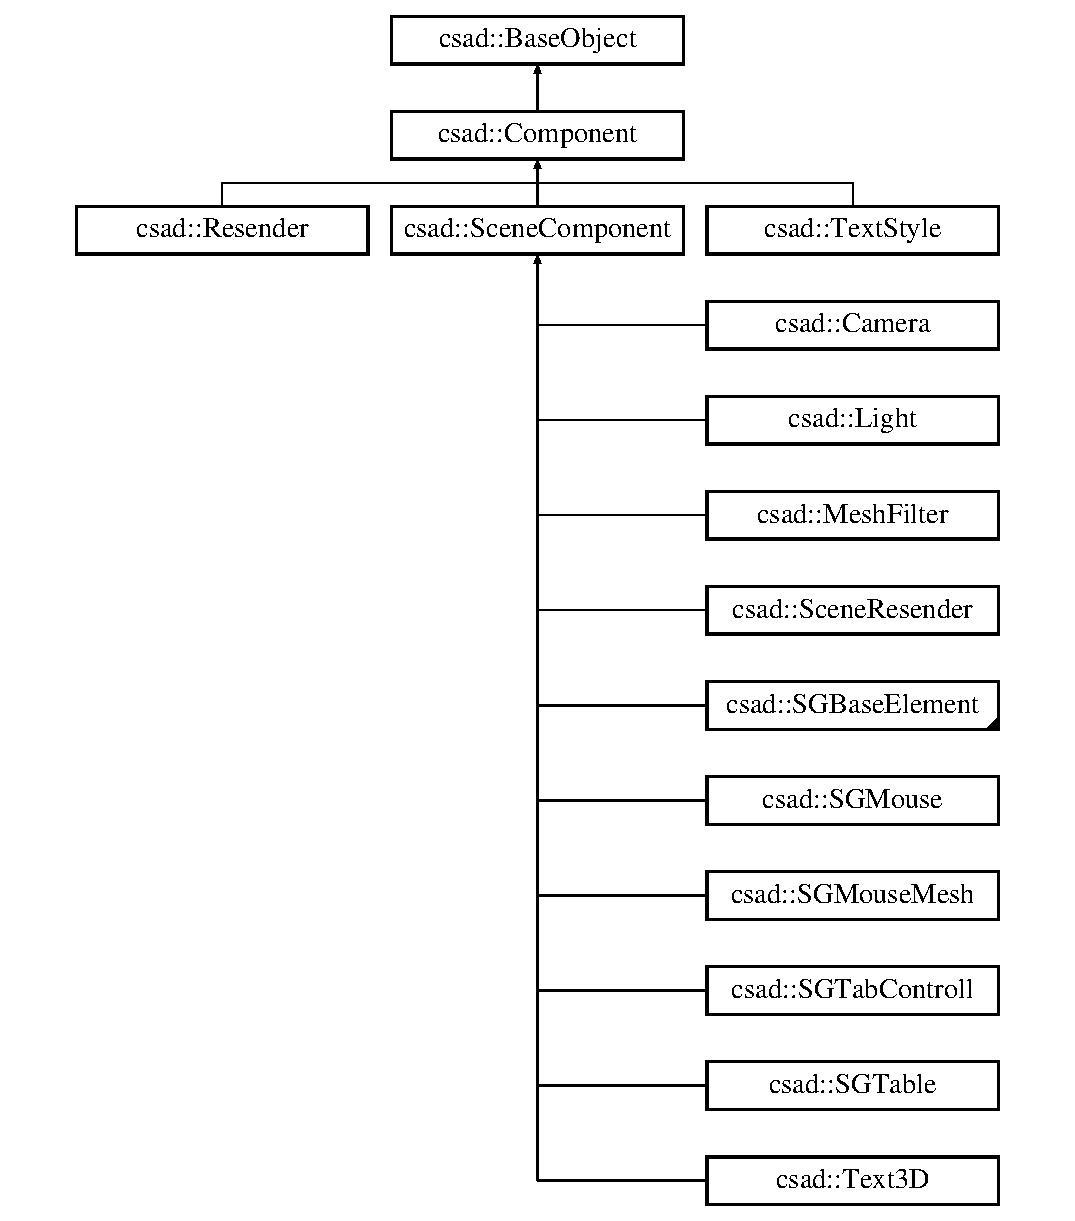
\includegraphics[height=12.000000cm]{classcsad_1_1_component}
\end{center}
\end{figure}
\subsection*{Public Member Functions}
\begin{DoxyCompactItemize}
\item 
\hypertarget{classcsad_1_1_component_ac35c5ad8712eb403c8bbc3c765f823b8}{{\footnotesize template$<$typename T $>$ }\\\-\_\-\-F\-O\-R\-C\-E\-I\-N\-L\-I\-N\-E T $\ast$ \hyperlink{classcsad_1_1_component_ac35c5ad8712eb403c8bbc3c765f823b8}{add\-Component} ()}\label{classcsad_1_1_component_ac35c5ad8712eb403c8bbc3c765f823b8}

\begin{DoxyCompactList}\small\item\em Add component of the specified type in the container if this component already exists, returns available. \end{DoxyCompactList}\item 
\hypertarget{classcsad_1_1_component_a3ec7ad4398b3b793561d84a7c3a3eef6}{{\footnotesize template$<$typename T $>$ }\\\-\_\-\-F\-O\-R\-C\-E\-I\-N\-L\-I\-N\-E T $\ast$ \hyperlink{classcsad_1_1_component_a3ec7ad4398b3b793561d84a7c3a3eef6}{get\-Component} ()}\label{classcsad_1_1_component_a3ec7ad4398b3b793561d84a7c3a3eef6}

\begin{DoxyCompactList}\small\item\em Returns the component of the given type, if it is not in a container returns 0. \end{DoxyCompactList}\item 
\hypertarget{classcsad_1_1_component_a00511e79db1c90f291e17b87c7e62696}{\-\_\-\-F\-O\-R\-C\-E\-I\-N\-L\-I\-N\-E \hyperlink{classcsad_1_1_container_components}{Container\-Components} $\ast$ \hyperlink{classcsad_1_1_component_a00511e79db1c90f291e17b87c7e62696}{get\-Container} ()}\label{classcsad_1_1_component_a00511e79db1c90f291e17b87c7e62696}

\begin{DoxyCompactList}\small\item\em Returns the container in which the component. \end{DoxyCompactList}\item 
\hypertarget{classcsad_1_1_component_ac5408f7b7ebe3b6b2141d4c7fb8146fe}{{\footnotesize template$<$typename T $>$ }\\\-\_\-\-F\-O\-R\-C\-E\-I\-N\-L\-I\-N\-E T $\ast$ \hyperlink{classcsad_1_1_component_ac5408f7b7ebe3b6b2141d4c7fb8146fe}{get\-Container} ()}\label{classcsad_1_1_component_ac5408f7b7ebe3b6b2141d4c7fb8146fe}

\begin{DoxyCompactList}\small\item\em Returns the container in which the component, if the container does not match the given type 0 is returned. \end{DoxyCompactList}\item 
\hypertarget{classcsad_1_1_component_a909c9fe50842ee5fbffee7cb5dde749b}{virtual C\-S\-A\-D\-\_\-\-A\-P\-I void \hyperlink{classcsad_1_1_component_a909c9fe50842ee5fbffee7cb5dde749b}{quit} ()}\label{classcsad_1_1_component_a909c9fe50842ee5fbffee7cb5dde749b}

\begin{DoxyCompactList}\small\item\em The event is called before the program exits. \end{DoxyCompactList}\item 
\hypertarget{classcsad_1_1_component_ad226c8f6c34ec780aaaedd087579ef0b}{C\-S\-A\-D\-\_\-\-A\-P\-I void $\ast$ \hyperlink{classcsad_1_1_component_ad226c8f6c34ec780aaaedd087579ef0b}{set} (unsigned \-\_\-int32, void $\ast$)}\label{classcsad_1_1_component_ad226c8f6c34ec780aaaedd087579ef0b}

\begin{DoxyCompactList}\small\item\em used for any interface commands. \end{DoxyCompactList}\item 
\hypertarget{classcsad_1_1_component_a79c83fa75a1ba6b6c3c53c8449ab14bb}{virtual C\-S\-A\-D\-\_\-\-A\-P\-I void \hyperlink{classcsad_1_1_component_a79c83fa75a1ba6b6c3c53c8449ab14bb}{start} ()}\label{classcsad_1_1_component_a79c83fa75a1ba6b6c3c53c8449ab14bb}

\begin{DoxyCompactList}\small\item\em This event is fired after the program start. \end{DoxyCompactList}\item 
\hypertarget{classcsad_1_1_component_a3e34aeff7ea26d56265237cbcf7a050c}{virtual C\-S\-A\-D\-\_\-\-A\-P\-I void \hyperlink{classcsad_1_1_component_a3e34aeff7ea26d56265237cbcf7a050c}{update} ()}\label{classcsad_1_1_component_a3e34aeff7ea26d56265237cbcf7a050c}

\begin{DoxyCompactList}\small\item\em This event is fired before rendering environment container component. \end{DoxyCompactList}\end{DoxyCompactItemize}
\subsection*{Static Public Member Functions}
\begin{DoxyCompactItemize}
\item 
static C\-S\-A\-D\-\_\-\-A\-P\-I int \hyperlink{classcsad_1_1_component_ac36baa797370264fac2a0dca02eb00d8}{reg\-Class} (const char $\ast$name, const void $\ast$info, tf\-S\-T\-D\-C\-A\-L\-L\-\_\-p\-\_\-\-F\-U\-N\-C\-\_\-p fun)
\end{DoxyCompactItemize}
\subsection*{Additional Inherited Members}


\subsection{Detailed Description}
\hyperlink{classcsad_1_1_component}{Component} -\/ a component is a unique part of the object may not have a name, and to exist independently. 

The component has a pointer to the container to which it belongs.

To register the component class there are two ways. To register in the module\-: \begin{DoxyVerb}  REG_COMPONENT(SomeClass)
\end{DoxyVerb}


To register the application\-: \begin{DoxyVerb}  COMPONENT_CLASS(SomeClass)

  void InitClass()
  {
     INIT_COMPONENT(SomeClass)
  }

  void main()
  {
     ...
     csadStart();
     InitClass();
     ...
  }
\end{DoxyVerb}


\begin{DoxySeeAlso}{See Also}
\hyperlink{group__core}{csad\-: core} 
\end{DoxySeeAlso}


\subsection{Member Function Documentation}
\hypertarget{classcsad_1_1_component_ac36baa797370264fac2a0dca02eb00d8}{\index{csad\-::\-Component@{csad\-::\-Component}!reg\-Class@{reg\-Class}}
\index{reg\-Class@{reg\-Class}!csad::Component@{csad\-::\-Component}}
\subsubsection[{reg\-Class}]{\setlength{\rightskip}{0pt plus 5cm}static C\-S\-A\-D\-\_\-\-A\-P\-I int csad\-::\-Component\-::reg\-Class (
\begin{DoxyParamCaption}
\item[{const char $\ast$}]{name, }
\item[{const void $\ast$}]{info, }
\item[{tf\-S\-T\-D\-C\-A\-L\-L\-\_\-p\-\_\-\-F\-U\-N\-C\-\_\-p}]{fun}
\end{DoxyParamCaption}
)\hspace{0.3cm}{\ttfamily [static]}}}\label{classcsad_1_1_component_ac36baa797370264fac2a0dca02eb00d8}
Registers the component class 
\begin{DoxyParams}{Parameters}
{\em name} & -\/ the class name of the component \\
\hline
{\em info} & -\/ the class identifier \\
\hline
{\em fun} & -\/ the class constructor \\
\hline
\end{DoxyParams}

\hypertarget{classcsad_1_1_config}{\section{csad\-:\-:Config Class Reference}
\label{classcsad_1_1_config}\index{csad\-::\-Config@{csad\-::\-Config}}
}


\hyperlink{classcsad_1_1_config}{Config} -\/ набор статических методов для формирования архитектуры приложения.  


\subsection*{Static Public Member Functions}
\begin{DoxyCompactItemize}
\item 
\hypertarget{classcsad_1_1_config_a9ca5275eadf123eaa7be8ccfc196673e}{static void \hyperlink{classcsad_1_1_config_a9ca5275eadf123eaa7be8ccfc196673e}{create\-From\-Xml} (\hyperlink{classcsad_1_1_format_x_m_l}{Format\-X\-M\-L} $\ast$xml)}\label{classcsad_1_1_config_a9ca5275eadf123eaa7be8ccfc196673e}

\begin{DoxyCompactList}\small\item\em формирование обьектов по конфигурации описанной в xml. \end{DoxyCompactList}\item 
\hypertarget{classcsad_1_1_config_a0e567ed8f9ccb211af175b0196894700}{static void \hyperlink{classcsad_1_1_config_a0e567ed8f9ccb211af175b0196894700}{init} ()}\label{classcsad_1_1_config_a0e567ed8f9ccb211af175b0196894700}

\begin{DoxyCompactList}\small\item\em инициализация \end{DoxyCompactList}\end{DoxyCompactItemize}


\subsection{Detailed Description}
\hyperlink{classcsad_1_1_config}{Config} -\/ набор статических методов для формирования архитектуры приложения. 

\begin{DoxySeeAlso}{See Also}
\hyperlink{group__core}{csad\-: core} 
\end{DoxySeeAlso}

\hypertarget{classcsad_1_1_container_components}{\section{csad\-:\-:Container\-Components Class Reference}
\label{classcsad_1_1_container_components}\index{csad\-::\-Container\-Components@{csad\-::\-Container\-Components}}
}


\hyperlink{classcsad_1_1_container_components}{Container\-Components} -\/ the container class components.  


Inheritance diagram for csad\-:\-:Container\-Components\-:\begin{figure}[H]
\begin{center}
\leavevmode
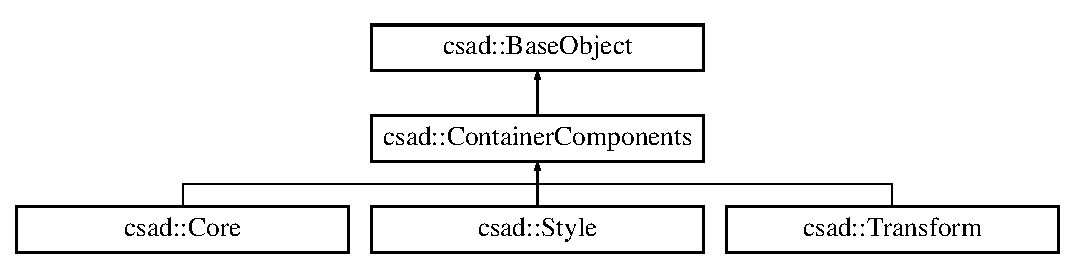
\includegraphics[height=3.000000cm]{classcsad_1_1_container_components}
\end{center}
\end{figure}
\subsection*{Public Member Functions}
\begin{DoxyCompactItemize}
\item 
\hypertarget{classcsad_1_1_container_components_a0e2225fc644c2c455edf632558b67343}{{\footnotesize template$<$typename T $>$ }\\\-\_\-\-F\-O\-R\-C\-E\-I\-N\-L\-I\-N\-E T $\ast$ \hyperlink{classcsad_1_1_container_components_a0e2225fc644c2c455edf632558b67343}{add\-Component} ()}\label{classcsad_1_1_container_components_a0e2225fc644c2c455edf632558b67343}

\begin{DoxyCompactList}\small\item\em Adds the component of the specified type in the container if this component already exists, returns available. \end{DoxyCompactList}\item 
\-\_\-\-F\-O\-R\-C\-E\-I\-N\-L\-I\-N\-E \hyperlink{classcsad_1_1_component}{Component} $\ast$ \hyperlink{classcsad_1_1_container_components_ad7f66892f1d0c60447414f6026deddda}{add\-Component} (char $\ast$name)
\item 
\-\_\-\-F\-O\-R\-C\-E\-I\-N\-L\-I\-N\-E \hyperlink{classcsad_1_1_component}{Component} $\ast$ \hyperlink{classcsad_1_1_container_components_af12ffafe06c2e3f6713ea59cf7415874}{add\-Component} (const char $\ast$name)
\item 
\hypertarget{classcsad_1_1_container_components_a7e0dc30d9108b3c5d8601fc74cbe38a2}{\-\_\-\-F\-O\-R\-C\-E\-I\-N\-L\-I\-N\-E iterator \hyperlink{classcsad_1_1_container_components_a7e0dc30d9108b3c5d8601fc74cbe38a2}{begin} ()}\label{classcsad_1_1_container_components_a7e0dc30d9108b3c5d8601fc74cbe38a2}

\begin{DoxyCompactList}\small\item\em The first element of the list of components. \end{DoxyCompactList}\item 
\hypertarget{classcsad_1_1_container_components_abc6cb7a65d3f7e5405376bd8ecb787dc}{{\footnotesize template$<$typename T $>$ }\\\-\_\-\-F\-O\-R\-C\-E\-I\-N\-L\-I\-N\-E void \hyperlink{classcsad_1_1_container_components_abc6cb7a65d3f7e5405376bd8ecb787dc}{delete\-Component} ()}\label{classcsad_1_1_container_components_abc6cb7a65d3f7e5405376bd8ecb787dc}

\begin{DoxyCompactList}\small\item\em Detaches the component from the container and remove the component. \end{DoxyCompactList}\item 
\hypertarget{classcsad_1_1_container_components_ae2fe8ab5f1842629656b154f62e81aa2}{\-\_\-\-F\-O\-R\-C\-E\-I\-N\-L\-I\-N\-E iterator \hyperlink{classcsad_1_1_container_components_ae2fe8ab5f1842629656b154f62e81aa2}{end} ()}\label{classcsad_1_1_container_components_ae2fe8ab5f1842629656b154f62e81aa2}

\begin{DoxyCompactList}\small\item\em The final element of the list component. \end{DoxyCompactList}\item 
\hypertarget{classcsad_1_1_container_components_a404e7d34ff05cf693f42c868fc272888}{\-\_\-\-F\-O\-R\-C\-E\-I\-N\-L\-I\-N\-E void \hyperlink{classcsad_1_1_container_components_a404e7d34ff05cf693f42c868fc272888}{free\-Components} ()}\label{classcsad_1_1_container_components_a404e7d34ff05cf693f42c868fc272888}

\begin{DoxyCompactList}\small\item\em detaches and removes components \end{DoxyCompactList}\item 
\hypertarget{classcsad_1_1_container_components_a6ae49f1007bcf86debe62b4024674fae}{{\footnotesize template$<$typename T $>$ }\\\-\_\-\-F\-O\-R\-C\-E\-I\-N\-L\-I\-N\-E T $\ast$ \hyperlink{classcsad_1_1_container_components_a6ae49f1007bcf86debe62b4024674fae}{get\-Component} ()}\label{classcsad_1_1_container_components_a6ae49f1007bcf86debe62b4024674fae}

\begin{DoxyCompactList}\small\item\em Returns the component of the given type, if it is not in a container returns 0. \end{DoxyCompactList}\item 
\hypertarget{classcsad_1_1_container_components_a7c0d7faa832475d9f8e8349dd6389ee2}{\-\_\-\-F\-O\-R\-C\-E\-I\-N\-L\-I\-N\-E \hyperlink{classcsad_1_1_component}{Component} $\ast$ \hyperlink{classcsad_1_1_container_components_a7c0d7faa832475d9f8e8349dd6389ee2}{get\-Component} (void $\ast$t)}\label{classcsad_1_1_container_components_a7c0d7faa832475d9f8e8349dd6389ee2}

\begin{DoxyCompactList}\small\item\em Returns the component of the given type, if it is not in a container returns 0. \end{DoxyCompactList}\item 
\-\_\-\-F\-O\-R\-C\-E\-I\-N\-L\-I\-N\-E \hyperlink{classcsad_1_1_component}{Component} $\ast$ \hyperlink{classcsad_1_1_container_components_a20e87b5dd1fb810997100f82c5da715d}{get\-Component} (char $\ast$name)
\item 
\-\_\-\-F\-O\-R\-C\-E\-I\-N\-L\-I\-N\-E \hyperlink{classcsad_1_1_component}{Component} $\ast$ \hyperlink{classcsad_1_1_container_components_ab3b09a7785fe6f0931f174c50912e52e}{get\-Component} (const char $\ast$name)
\item 
\hypertarget{classcsad_1_1_container_components_a48f1bed785f23be756a477ed638fa3b5}{\-\_\-\-F\-O\-R\-C\-E\-I\-N\-L\-I\-N\-E \hyperlink{classbt_1_1_map_void}{Components\-Map} \& \hyperlink{classcsad_1_1_container_components_a48f1bed785f23be756a477ed638fa3b5}{list} ()}\label{classcsad_1_1_container_components_a48f1bed785f23be756a477ed638fa3b5}

\begin{DoxyCompactList}\small\item\em Returns list of Components. \end{DoxyCompactList}\item 
\hypertarget{classcsad_1_1_container_components_a2cdd24762a2fcf66fab366172bff6527}{virtual C\-S\-A\-D\-\_\-\-A\-P\-I void \hyperlink{classcsad_1_1_container_components_a2cdd24762a2fcf66fab366172bff6527}{quit} ()}\label{classcsad_1_1_container_components_a2cdd24762a2fcf66fab366172bff6527}

\begin{DoxyCompactList}\small\item\em Transfers control to the nested components quit calling each of them. \end{DoxyCompactList}\item 
\hypertarget{classcsad_1_1_container_components_ad28a786b0fa5089944ec7335e5358951}{{\footnotesize template$<$typename T $>$ }\\\-\_\-\-F\-O\-R\-C\-E\-I\-N\-L\-I\-N\-E void \hyperlink{classcsad_1_1_container_components_ad28a786b0fa5089944ec7335e5358951}{remove\-Component} ()}\label{classcsad_1_1_container_components_ad28a786b0fa5089944ec7335e5358951}

\begin{DoxyCompactList}\small\item\em Detaches the component from a container. \end{DoxyCompactList}\item 
\hypertarget{classcsad_1_1_container_components_a5e464c03fe5ea072f7887ff839831fe8}{C\-S\-A\-D\-\_\-\-A\-P\-I void $\ast$ \hyperlink{classcsad_1_1_container_components_a5e464c03fe5ea072f7887ff839831fe8}{set} (unsigned \-\_\-int32, void $\ast$)}\label{classcsad_1_1_container_components_a5e464c03fe5ea072f7887ff839831fe8}

\begin{DoxyCompactList}\small\item\em used for any interface commands. \end{DoxyCompactList}\item 
C\-S\-A\-D\-\_\-\-A\-P\-I void $\ast$ \hyperlink{classcsad_1_1_container_components_a3c373a98a6981e002151a7cd1e1c89c8}{set\-Components} (unsigned int id, void $\ast$param)
\item 
\hypertarget{classcsad_1_1_container_components_a63b01a1010a04844579bb9d011283e05}{virtual C\-S\-A\-D\-\_\-\-A\-P\-I void \hyperlink{classcsad_1_1_container_components_a63b01a1010a04844579bb9d011283e05}{start} ()}\label{classcsad_1_1_container_components_a63b01a1010a04844579bb9d011283e05}

\begin{DoxyCompactList}\small\item\em Transfers control to the nested components start calling each of them. \end{DoxyCompactList}\item 
\hypertarget{classcsad_1_1_container_components_a5ea5732bcd86cdb9c745cb323ee9c4af}{virtual C\-S\-A\-D\-\_\-\-A\-P\-I void \hyperlink{classcsad_1_1_container_components_a5ea5732bcd86cdb9c745cb323ee9c4af}{update} ()}\label{classcsad_1_1_container_components_a5ea5732bcd86cdb9c745cb323ee9c4af}

\begin{DoxyCompactList}\small\item\em Transfers control to the nested components causing update each of them. \end{DoxyCompactList}\end{DoxyCompactItemize}
\subsection*{Static Public Member Functions}
\begin{DoxyCompactItemize}
\item 
static C\-S\-A\-D\-\_\-\-A\-P\-I int \hyperlink{classcsad_1_1_container_components_ac09864fc54d500377e5df6b095f5f2c7}{reg\-Class} (const char $\ast$name, const void $\ast$info, tf\-S\-T\-D\-C\-A\-L\-L\-\_\-p\-\_\-\-F\-U\-N\-C\-\_\-p fun)
\end{DoxyCompactItemize}
\subsection*{Additional Inherited Members}


\subsection{Detailed Description}
\hyperlink{classcsad_1_1_container_components}{Container\-Components} -\/ the container class components. 

The container has a map of pointers to objects components.

\begin{DoxySeeAlso}{See Also}
\hyperlink{group__core}{csad\-: core} 
\end{DoxySeeAlso}


\subsection{Member Function Documentation}
\hypertarget{classcsad_1_1_container_components_ad7f66892f1d0c60447414f6026deddda}{\index{csad\-::\-Container\-Components@{csad\-::\-Container\-Components}!add\-Component@{add\-Component}}
\index{add\-Component@{add\-Component}!csad::ContainerComponents@{csad\-::\-Container\-Components}}
\subsubsection[{add\-Component}]{\setlength{\rightskip}{0pt plus 5cm}\-\_\-\-F\-O\-R\-C\-E\-I\-N\-L\-I\-N\-E {\bf Component}$\ast$ csad\-::\-Container\-Components\-::add\-Component (
\begin{DoxyParamCaption}
\item[{char $\ast$}]{name}
\end{DoxyParamCaption}
)\hspace{0.3cm}{\ttfamily [inline]}}}\label{classcsad_1_1_container_components_ad7f66892f1d0c60447414f6026deddda}
Create a component class name and adds it to the container. 
\begin{DoxyParams}{Parameters}
{\em name} & -\/ the name of the component class. \\
\hline
\end{DoxyParams}
\begin{DoxyReturn}{Returns}
a new component, or available in the container 
\end{DoxyReturn}
\hypertarget{classcsad_1_1_container_components_af12ffafe06c2e3f6713ea59cf7415874}{\index{csad\-::\-Container\-Components@{csad\-::\-Container\-Components}!add\-Component@{add\-Component}}
\index{add\-Component@{add\-Component}!csad::ContainerComponents@{csad\-::\-Container\-Components}}
\subsubsection[{add\-Component}]{\setlength{\rightskip}{0pt plus 5cm}\-\_\-\-F\-O\-R\-C\-E\-I\-N\-L\-I\-N\-E {\bf Component}$\ast$ csad\-::\-Container\-Components\-::add\-Component (
\begin{DoxyParamCaption}
\item[{const char $\ast$}]{name}
\end{DoxyParamCaption}
)\hspace{0.3cm}{\ttfamily [inline]}}}\label{classcsad_1_1_container_components_af12ffafe06c2e3f6713ea59cf7415874}
Creates a component class name and add it to the container, if the component is already contained in the container is returned to the available component 
\begin{DoxyParams}{Parameters}
{\em name} & -\/ the name of the component class. \\
\hline
\end{DoxyParams}
\begin{DoxyReturn}{Returns}
a new component, or available in the container 
\end{DoxyReturn}
\hypertarget{classcsad_1_1_container_components_a20e87b5dd1fb810997100f82c5da715d}{\index{csad\-::\-Container\-Components@{csad\-::\-Container\-Components}!get\-Component@{get\-Component}}
\index{get\-Component@{get\-Component}!csad::ContainerComponents@{csad\-::\-Container\-Components}}
\subsubsection[{get\-Component}]{\setlength{\rightskip}{0pt plus 5cm}\-\_\-\-F\-O\-R\-C\-E\-I\-N\-L\-I\-N\-E {\bf Component}$\ast$ csad\-::\-Container\-Components\-::get\-Component (
\begin{DoxyParamCaption}
\item[{char $\ast$}]{name}
\end{DoxyParamCaption}
)\hspace{0.3cm}{\ttfamily [inline]}}}\label{classcsad_1_1_container_components_a20e87b5dd1fb810997100f82c5da715d}
Returns the component of the specified class. 
\begin{DoxyParams}{Parameters}
{\em name} & -\/ the name of the component class. \\
\hline
\end{DoxyParams}
\begin{DoxyReturn}{Returns}
the component is available in a container, or null if it is not. 
\end{DoxyReturn}
\hypertarget{classcsad_1_1_container_components_ab3b09a7785fe6f0931f174c50912e52e}{\index{csad\-::\-Container\-Components@{csad\-::\-Container\-Components}!get\-Component@{get\-Component}}
\index{get\-Component@{get\-Component}!csad::ContainerComponents@{csad\-::\-Container\-Components}}
\subsubsection[{get\-Component}]{\setlength{\rightskip}{0pt plus 5cm}\-\_\-\-F\-O\-R\-C\-E\-I\-N\-L\-I\-N\-E {\bf Component}$\ast$ csad\-::\-Container\-Components\-::get\-Component (
\begin{DoxyParamCaption}
\item[{const char $\ast$}]{name}
\end{DoxyParamCaption}
)\hspace{0.3cm}{\ttfamily [inline]}}}\label{classcsad_1_1_container_components_ab3b09a7785fe6f0931f174c50912e52e}
Returns the component of the specified class. 
\begin{DoxyParams}{Parameters}
{\em name} & -\/ the name of the component class. \\
\hline
\end{DoxyParams}
\begin{DoxyReturn}{Returns}
the component is available in a container, or null if it is not. 
\end{DoxyReturn}
\hypertarget{classcsad_1_1_container_components_ac09864fc54d500377e5df6b095f5f2c7}{\index{csad\-::\-Container\-Components@{csad\-::\-Container\-Components}!reg\-Class@{reg\-Class}}
\index{reg\-Class@{reg\-Class}!csad::ContainerComponents@{csad\-::\-Container\-Components}}
\subsubsection[{reg\-Class}]{\setlength{\rightskip}{0pt plus 5cm}static C\-S\-A\-D\-\_\-\-A\-P\-I int csad\-::\-Container\-Components\-::reg\-Class (
\begin{DoxyParamCaption}
\item[{const char $\ast$}]{name, }
\item[{const void $\ast$}]{info, }
\item[{tf\-S\-T\-D\-C\-A\-L\-L\-\_\-p\-\_\-\-F\-U\-N\-C\-\_\-p}]{fun}
\end{DoxyParamCaption}
)\hspace{0.3cm}{\ttfamily [static]}}}\label{classcsad_1_1_container_components_ac09864fc54d500377e5df6b095f5f2c7}
Registers the component class 
\begin{DoxyParams}{Parameters}
{\em name} & -\/ the class name of the component \\
\hline
{\em info} & -\/ the class identifier \\
\hline
{\em fun} & -\/ the class identifier \\
\hline
\end{DoxyParams}
\hypertarget{classcsad_1_1_container_components_a3c373a98a6981e002151a7cd1e1c89c8}{\index{csad\-::\-Container\-Components@{csad\-::\-Container\-Components}!set\-Components@{set\-Components}}
\index{set\-Components@{set\-Components}!csad::ContainerComponents@{csad\-::\-Container\-Components}}
\subsubsection[{set\-Components}]{\setlength{\rightskip}{0pt plus 5cm}C\-S\-A\-D\-\_\-\-A\-P\-I void$\ast$ csad\-::\-Container\-Components\-::set\-Components (
\begin{DoxyParamCaption}
\item[{unsigned int}]{id, }
\item[{void $\ast$}]{param}
\end{DoxyParamCaption}
)}}\label{classcsad_1_1_container_components_a3c373a98a6981e002151a7cd1e1c89c8}
Passes the components parameters from the \hyperlink{classcsad_1_1_base_object_aa8d3a855874527b14a5c56f629789b1f}{Base\-Object\-::set}. 
\begin{DoxyParams}{Parameters}
{\em id} & -\/ id Base\-Object\-::\-Base \\
\hline
{\em param} & -\/ a pointer to a structure parameters. \\
\hline
\end{DoxyParams}
\begin{DoxyReturn}{Returns}
depends on id. 
\end{DoxyReturn}

\hypertarget{classcsad_1_1_core}{\section{csad\-:\-:Core Class Reference}
\label{classcsad_1_1_core}\index{csad\-::\-Core@{csad\-::\-Core}}
}


\hyperlink{classcsad_1_1_core}{Core} -\/ the Manager interface of the application.  


Inheritance diagram for csad\-:\-:Core\-:\begin{figure}[H]
\begin{center}
\leavevmode
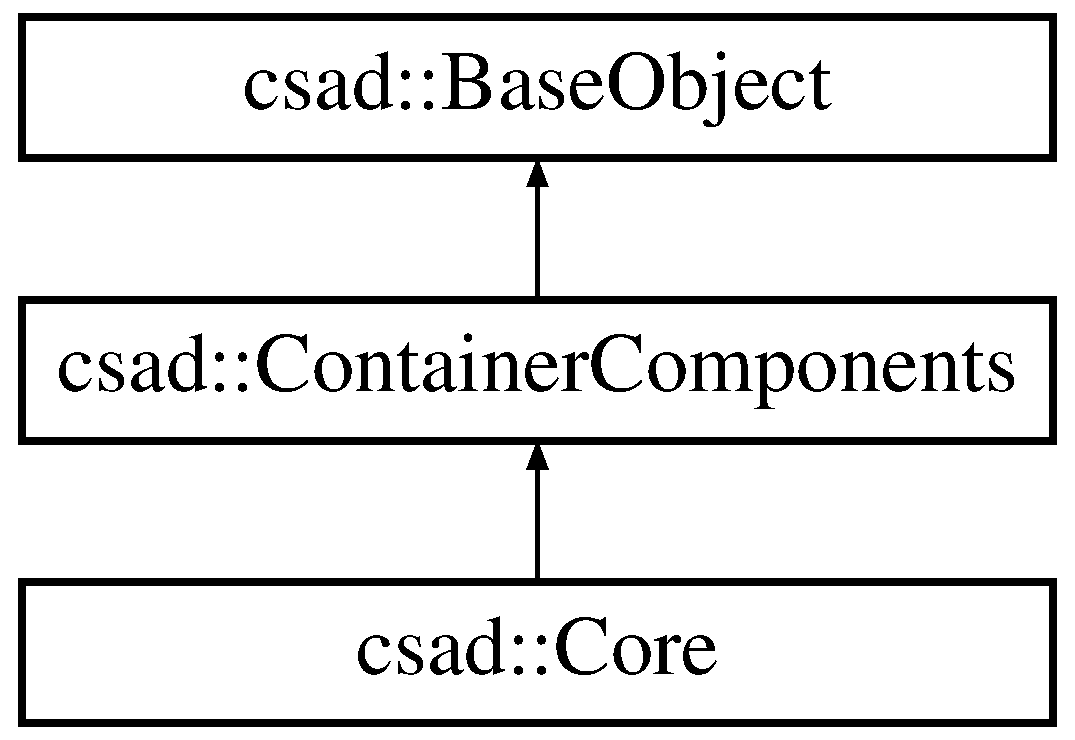
\includegraphics[height=3.000000cm]{classcsad_1_1_core}
\end{center}
\end{figure}
\subsection*{Public Member Functions}
\begin{DoxyCompactItemize}
\item 
\hypertarget{classcsad_1_1_core_a8ed42063dccc8a04d02ec7c7c12e631d}{\-\_\-\-F\-O\-R\-C\-E\-I\-N\-L\-I\-N\-E \hyperlink{classcsad_1_1_class_manager}{Class\-Manager} $\ast$ \hyperlink{classcsad_1_1_core_a8ed42063dccc8a04d02ec7c7c12e631d}{class\-Manager} ()}\label{classcsad_1_1_core_a8ed42063dccc8a04d02ec7c7c12e631d}

\begin{DoxyCompactList}\small\item\em Manager classes. \end{DoxyCompactList}\item 
\hypertarget{classcsad_1_1_core_a8fddcefd07424ba6b09e5732c44cde57}{\-\_\-\-F\-O\-R\-C\-E\-I\-N\-L\-I\-N\-E \hyperlink{classcsad_1_1_graph}{Graph} $\ast$ \hyperlink{classcsad_1_1_core_a8fddcefd07424ba6b09e5732c44cde57}{graph} ()}\label{classcsad_1_1_core_a8fddcefd07424ba6b09e5732c44cde57}

\begin{DoxyCompactList}\small\item\em Manager graphical elements. \end{DoxyCompactList}\item 
\hypertarget{classcsad_1_1_core_aae3c05a0d844dd7d2091959937c915ff}{\-\_\-\-F\-O\-R\-C\-E\-I\-N\-L\-I\-N\-E \hyperlink{classcsad_1_1_input}{Input} $\ast$ \hyperlink{classcsad_1_1_core_aae3c05a0d844dd7d2091959937c915ff}{input} ()}\label{classcsad_1_1_core_aae3c05a0d844dd7d2091959937c915ff}

\begin{DoxyCompactList}\small\item\em The Manager of the input systems. \end{DoxyCompactList}\item 
\hypertarget{classcsad_1_1_core_a1afeb01a16e7286c9801405eb7211e3c}{M\-E\-M\-N\-U\-L\-L \-\_\-\-F\-O\-R\-C\-E\-I\-N\-L\-I\-N\-E \\*
\hyperlink{classcsad_1_1_object_manager}{Object\-Manager} $\ast$ \hyperlink{classcsad_1_1_core_a1afeb01a16e7286c9801405eb7211e3c}{manager} ()}\label{classcsad_1_1_core_a1afeb01a16e7286c9801405eb7211e3c}

\begin{DoxyCompactList}\small\item\em the root object Manager \end{DoxyCompactList}\item 
\hypertarget{classcsad_1_1_core_a618ee56f40d4e272e5af92aef115becf}{virtual void \hyperlink{classcsad_1_1_core_a618ee56f40d4e272e5af92aef115becf}{quit} ()=0}\label{classcsad_1_1_core_a618ee56f40d4e272e5af92aef115becf}

\begin{DoxyCompactList}\small\item\em Transfers control to the nested components quit calling each of them. \end{DoxyCompactList}\item 
\hypertarget{classcsad_1_1_core_a5a91731a8393443e70107d01cc1251f4}{virtual void \hyperlink{classcsad_1_1_core_a5a91731a8393443e70107d01cc1251f4}{start} ()=0}\label{classcsad_1_1_core_a5a91731a8393443e70107d01cc1251f4}

\begin{DoxyCompactList}\small\item\em Transfers control to the nested components start calling each of them. \end{DoxyCompactList}\item 
\hypertarget{classcsad_1_1_core_aca7459f5c5bd54d7e27841add759bfac}{\-\_\-\-F\-O\-R\-C\-E\-I\-N\-L\-I\-N\-E \hyperlink{classcsad_1_1_system}{System} $\ast$ \hyperlink{classcsad_1_1_core_aca7459f5c5bd54d7e27841add759bfac}{system} ()}\label{classcsad_1_1_core_aca7459f5c5bd54d7e27841add759bfac}

\begin{DoxyCompactList}\small\item\em the Manager of system objects \end{DoxyCompactList}\item 
\hypertarget{classcsad_1_1_core_ac2f2c39bca8736c4fb0888b64e496971}{\-\_\-\-F\-O\-R\-C\-E\-I\-N\-L\-I\-N\-E \hyperlink{classcsad_1_1_timer}{Timer} \& \hyperlink{classcsad_1_1_core_ac2f2c39bca8736c4fb0888b64e496971}{timer} ()}\label{classcsad_1_1_core_ac2f2c39bca8736c4fb0888b64e496971}

\begin{DoxyCompactList}\small\item\em timer \end{DoxyCompactList}\end{DoxyCompactItemize}
\subsection*{Static Public Member Functions}
\begin{DoxyCompactItemize}
\item 
\hypertarget{classcsad_1_1_core_a7516bdeb9a403d71b5a05525ec60ac11}{static \-\_\-\-F\-O\-R\-C\-E\-I\-N\-L\-I\-N\-E \hyperlink{classcsad_1_1_core}{Core} $\ast$ \hyperlink{classcsad_1_1_core_a7516bdeb9a403d71b5a05525ec60ac11}{Create} ()}\label{classcsad_1_1_core_a7516bdeb9a403d71b5a05525ec60ac11}

\begin{DoxyCompactList}\small\item\em creates the environment \end{DoxyCompactList}\item 
\hypertarget{classcsad_1_1_core_a2cf4e6338c71fb343356c751fc85cadd}{static \-\_\-\-F\-O\-R\-C\-E\-I\-N\-L\-I\-N\-E \hyperlink{classcsad_1_1_core}{Core} \& \hyperlink{classcsad_1_1_core_a2cf4e6338c71fb343356c751fc85cadd}{current} ()}\label{classcsad_1_1_core_a2cf4e6338c71fb343356c751fc85cadd}

\begin{DoxyCompactList}\small\item\em returns the current environment \end{DoxyCompactList}\item 
\hypertarget{classcsad_1_1_core_a8d1bf53f8baa7c6c92e24528e31c2877}{static \-\_\-\-F\-O\-R\-C\-E\-I\-N\-L\-I\-N\-E void \hyperlink{classcsad_1_1_core_a8d1bf53f8baa7c6c92e24528e31c2877}{set} (\hyperlink{classcsad_1_1_core}{Core} $\ast$core)}\label{classcsad_1_1_core_a8d1bf53f8baa7c6c92e24528e31c2877}

\begin{DoxyCompactList}\small\item\em sets the active environment \end{DoxyCompactList}\end{DoxyCompactItemize}
\subsection*{Additional Inherited Members}


\subsection{Detailed Description}
\hyperlink{classcsad_1_1_core}{Core} -\/ the Manager interface of the application. 

\begin{DoxySeeAlso}{See Also}
\hyperlink{group__core}{csad\-: core} 
\end{DoxySeeAlso}

\hypertarget{classcsad_1_1_display}{\section{csad\-:\-:Display Class Reference}
\label{classcsad_1_1_display}\index{csad\-::\-Display@{csad\-::\-Display}}
}


\hyperlink{classcsad_1_1_display}{Display} -\/ the class of the output device.  


Inheritance diagram for csad\-:\-:Display\-:\begin{figure}[H]
\begin{center}
\leavevmode
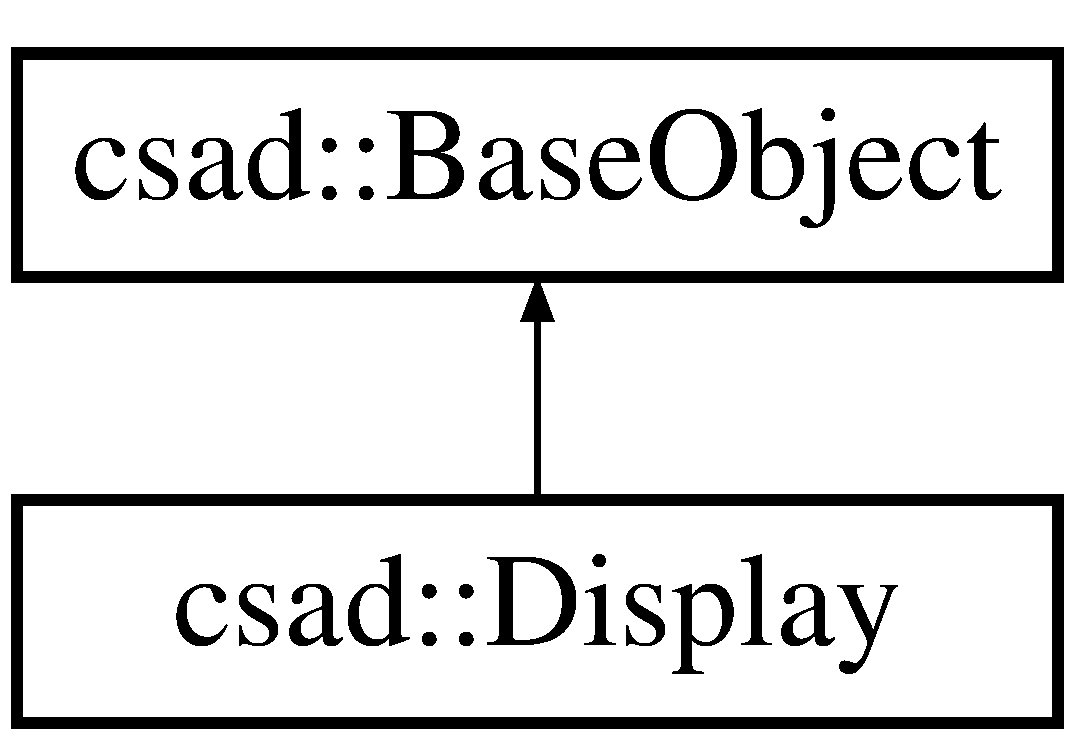
\includegraphics[height=2.000000cm]{classcsad_1_1_display}
\end{center}
\end{figure}
\subsection*{Public Member Functions}
\begin{DoxyCompactItemize}
\item 
\hypertarget{classcsad_1_1_display_a20d187bd432fe8a53becfcf217f90029}{\-\_\-\-F\-O\-R\-C\-E\-I\-N\-L\-I\-N\-E \hyperlink{classcsad_1_1_gl_context}{Gl\-Context} $\ast$ \hyperlink{classcsad_1_1_display_a20d187bd432fe8a53becfcf217f90029}{create\-Context} (const char $\ast$name=\char`\"{}\char`\"{})}\label{classcsad_1_1_display_a20d187bd432fe8a53becfcf217f90029}

\begin{DoxyCompactList}\small\item\em create new context. \end{DoxyCompactList}\item 
\hypertarget{classcsad_1_1_display_aac6a3e516fe763e61fc6ddfeb130a8fb}{virtual \hyperlink{classcsad_1_1_gl_context}{Gl\-Context} $\ast$ \hyperlink{classcsad_1_1_display_aac6a3e516fe763e61fc6ddfeb130a8fb}{get\-Context} (char $\ast$)=0}\label{classcsad_1_1_display_aac6a3e516fe763e61fc6ddfeb130a8fb}

\begin{DoxyCompactList}\small\item\em Returns the context by name. \end{DoxyCompactList}\item 
\hypertarget{classcsad_1_1_display_a094ceb34dedd1d75b173cadf5bd00be3}{virtual void $\ast$ \hyperlink{classcsad_1_1_display_a094ceb34dedd1d75b173cadf5bd00be3}{get\-Handle} ()=0}\label{classcsad_1_1_display_a094ceb34dedd1d75b173cadf5bd00be3}

\begin{DoxyCompactList}\small\item\em return handle of device \end{DoxyCompactList}\item 
\hypertarget{classcsad_1_1_display_a6146300090d3c7fdb002b10b6259e45a}{virtual \-\_\-int32 \hyperlink{classcsad_1_1_display_a6146300090d3c7fdb002b10b6259e45a}{height} ()=0}\label{classcsad_1_1_display_a6146300090d3c7fdb002b10b6259e45a}

\begin{DoxyCompactList}\small\item\em the height of the screen \end{DoxyCompactList}\item 
\hypertarget{classcsad_1_1_display_ae56edf18d46dd676e5123936a6c35d84}{virtual bool \hyperlink{classcsad_1_1_display_ae56edf18d46dd676e5123936a6c35d84}{is\-Global\-Point} (\hyperlink{classbt_1_1vector2i}{vector2i} $\ast$pos)=0}\label{classcsad_1_1_display_ae56edf18d46dd676e5123936a6c35d84}

\begin{DoxyCompactList}\small\item\em Crossing checking the global coordinates of the screen with display. \end{DoxyCompactList}\item 
\hypertarget{classcsad_1_1_display_a26d239250ad328c5ed9ff7186753f015}{\-\_\-\-F\-O\-R\-C\-E\-I\-N\-L\-I\-N\-E bool \hyperlink{classcsad_1_1_display_a26d239250ad328c5ed9ff7186753f015}{is\-V\-Sync} ()}\label{classcsad_1_1_display_a26d239250ad328c5ed9ff7186753f015}

\begin{DoxyCompactList}\small\item\em Checking mode vertical sync. \end{DoxyCompactList}\item 
\hypertarget{classcsad_1_1_display_a8685f55f9af5bacbb512f4f65347fbdc}{virtual \-\_\-int32 \hyperlink{classcsad_1_1_display_a8685f55f9af5bacbb512f4f65347fbdc}{left} ()=0}\label{classcsad_1_1_display_a8685f55f9af5bacbb512f4f65347fbdc}

\begin{DoxyCompactList}\small\item\em The left position of the screen in desktop coordinate system. \end{DoxyCompactList}\item 
\hypertarget{classcsad_1_1_display_aa13dbec69c7ad3b4025a9f0ff958e276}{\-\_\-\-F\-O\-R\-C\-E\-I\-N\-L\-I\-N\-E void \hyperlink{classcsad_1_1_display_aa13dbec69c7ad3b4025a9f0ff958e276}{Set\-V\-Sync} (bool val)}\label{classcsad_1_1_display_aa13dbec69c7ad3b4025a9f0ff958e276}

\begin{DoxyCompactList}\small\item\em Setting of a mode vertical sync. \end{DoxyCompactList}\item 
\hypertarget{classcsad_1_1_display_aa16c4a6dd845993283871a224a67511f}{\-\_\-\-F\-O\-R\-C\-E\-I\-N\-L\-I\-N\-E void \hyperlink{classcsad_1_1_display_aa16c4a6dd845993283871a224a67511f}{Set\-Windowed} (bool val)}\label{classcsad_1_1_display_aa16c4a6dd845993283871a224a67511f}

\begin{DoxyCompactList}\small\item\em Setting of a mode window/fullscreen. \end{DoxyCompactList}\item 
\hypertarget{classcsad_1_1_display_a3ac4c7a9a4585d709fb5b434c64429d9}{virtual \-\_\-int32 \hyperlink{classcsad_1_1_display_a3ac4c7a9a4585d709fb5b434c64429d9}{top} ()=0}\label{classcsad_1_1_display_a3ac4c7a9a4585d709fb5b434c64429d9}

\begin{DoxyCompactList}\small\item\em The top position of the screen in desktop coordinate system. \end{DoxyCompactList}\item 
\hypertarget{classcsad_1_1_display_a8c58cdfa8d73d88cfd46043cc0433218}{virtual \-\_\-int32 \hyperlink{classcsad_1_1_display_a8c58cdfa8d73d88cfd46043cc0433218}{width} ()=0}\label{classcsad_1_1_display_a8c58cdfa8d73d88cfd46043cc0433218}

\begin{DoxyCompactList}\small\item\em the width of the screen \end{DoxyCompactList}\end{DoxyCompactItemize}
\subsection*{Additional Inherited Members}


\subsection{Detailed Description}
\hyperlink{classcsad_1_1_display}{Display} -\/ the class of the output device. 

In different ways this can be separately selected output device or the output window. When using operating systems support window organization applications, you can specify the mode display full screen or windowed. To specify the mode of displaying the image indicated ...

\begin{DoxyVerb}  <Scene name="the name of the scene">
  <Display name="" dev="the logical number of the controller" id="logical device number" mode="fullscreen/windowed" render="soft/gl/gles">
      ...
  </Display>
\end{DoxyVerb}


\begin{DoxySeeAlso}{See Also}
\hyperlink{group__scene}{csad\-: scene} 
\end{DoxySeeAlso}

\hypertarget{classcsad_1_1_file}{\section{csad\-:\-:File Class Reference}
\label{classcsad_1_1_file}\index{csad\-::\-File@{csad\-::\-File}}
}


\hyperlink{classcsad_1_1_file}{File} -\/ A file object.  


\subsection*{Public Types}
\begin{DoxyCompactItemize}
\item 
enum \hyperlink{classcsad_1_1_file_a0c256c83ef20258eb8d22826e5915d5a}{I\-O\-Type} \{ \\*
\hyperlink{classcsad_1_1_file_a0c256c83ef20258eb8d22826e5915d5aad43f934455c63c17c3fb53cfe87eb4c8}{R\-E\-A\-D}, 
\hyperlink{classcsad_1_1_file_a0c256c83ef20258eb8d22826e5915d5aa297c373b4f92bf6a3586bdffe5c7ae7e}{W\-R\-I\-T\-E}, 
\hyperlink{classcsad_1_1_file_a0c256c83ef20258eb8d22826e5915d5aa98b61d0244be5ae4a22f32e37587a339}{R\-E\-A\-D\-W\-R\-I\-T\-E}, 
\hyperlink{classcsad_1_1_file_a0c256c83ef20258eb8d22826e5915d5aad0cc31e4c4e141695820637b226c30b5}{C\-R\-E\-A\-T\-E}, 
\\*
\hyperlink{classcsad_1_1_file_a0c256c83ef20258eb8d22826e5915d5aa6bc34ec5986a01f26fe2f71ba41e7fbb}{C\-R\-E\-A\-T\-E\-R\-W}
 \}
\item 
enum \hyperlink{classcsad_1_1_file_aec12a732c41b7586f7bff0925b4deb97}{Pos\-From} \{ \hyperlink{classcsad_1_1_file_aec12a732c41b7586f7bff0925b4deb97a4e995e5b070608e33741709308793835}{B\-E\-G\-I\-N}, 
\hyperlink{classcsad_1_1_file_aec12a732c41b7586f7bff0925b4deb97a61b4d3f9c0706ff9b3a4ee2f177c1edb}{C\-U\-R\-R\-E\-N\-T}, 
\hyperlink{classcsad_1_1_file_aec12a732c41b7586f7bff0925b4deb97a9ca1c0d65d2bdb2a970afabe96303609}{E\-N\-D}
 \}
\end{DoxyCompactItemize}
\subsection*{Public Member Functions}
\begin{DoxyCompactItemize}
\item 
\hypertarget{classcsad_1_1_file_a4319b35b4fdc39d2fa1c539959f6c325}{P\-L\-A\-T\-F\-O\-R\-M\-\_\-\-A\-P\-I \hyperlink{classcsad_1_1_file_a4319b35b4fdc39d2fa1c539959f6c325}{File} (\hyperlink{classcsad_1_1_file_a0c256c83ef20258eb8d22826e5915d5a}{I\-O\-Type} io)}\label{classcsad_1_1_file_a4319b35b4fdc39d2fa1c539959f6c325}

\begin{DoxyCompactList}\small\item\em Конструктор \end{DoxyCompactList}\item 
\hypertarget{classcsad_1_1_file_aa5258554865f47eea4e5d91c4654804e}{P\-L\-A\-T\-F\-O\-R\-M\-\_\-\-A\-P\-I \hyperlink{classcsad_1_1_file_aa5258554865f47eea4e5d91c4654804e}{File} (char $\ast$name, \hyperlink{classcsad_1_1_file_a0c256c83ef20258eb8d22826e5915d5a}{I\-O\-Type} io=\hyperlink{classcsad_1_1_file_a0c256c83ef20258eb8d22826e5915d5aad43f934455c63c17c3fb53cfe87eb4c8}{R\-E\-A\-D})}\label{classcsad_1_1_file_aa5258554865f47eea4e5d91c4654804e}

\begin{DoxyCompactList}\small\item\em Конструктор \end{DoxyCompactList}\item 
P\-L\-A\-T\-F\-O\-R\-M\-\_\-\-A\-P\-I bool \hyperlink{classcsad_1_1_file_a5d0d38b7bf4963f0d75e7fe82dfee8e2}{close} ()
\begin{DoxyCompactList}\small\item\em closes the file \end{DoxyCompactList}\item 
\-\_\-\-F\-O\-R\-C\-E\-I\-N\-L\-I\-N\-E void $\ast$ \hyperlink{classcsad_1_1_file_a9a11f812d37f46e6cfa3e602cb13149e}{get\-Header} ()
\item 
P\-L\-A\-T\-F\-O\-R\-M\-\_\-\-A\-P\-I bool \hyperlink{classcsad_1_1_file_a16421c80ec0fef10daaafba08c8ebf86}{open} ()
\begin{DoxyCompactList}\small\item\em opens or creates a new file \end{DoxyCompactList}\item 
P\-L\-A\-T\-F\-O\-R\-M\-\_\-\-A\-P\-I int \hyperlink{classcsad_1_1_file_a25704302675d9557d3095e7280aa1975}{read} (void $\ast$data, int count)
\begin{DoxyCompactList}\small\item\em read block of data from a file \end{DoxyCompactList}\item 
\hypertarget{classcsad_1_1_file_afdc838f028cebf2dcc200571d50fddb7}{P\-L\-A\-T\-F\-O\-R\-M\-\_\-\-A\-P\-I char $\ast$ \hyperlink{classcsad_1_1_file_afdc838f028cebf2dcc200571d50fddb7}{read\-All} ()}\label{classcsad_1_1_file_afdc838f028cebf2dcc200571d50fddb7}

\begin{DoxyCompactList}\small\item\em создает буфер разбером в файл и читает из него все содержимое \end{DoxyCompactList}\item 
\hypertarget{classcsad_1_1_file_ae7a246a527ba8244fed41306e792b378}{P\-L\-A\-T\-F\-O\-R\-M\-\_\-\-A\-P\-I void \hyperlink{classcsad_1_1_file_ae7a246a527ba8244fed41306e792b378}{set\-File\-Name} (char $\ast$)}\label{classcsad_1_1_file_ae7a246a527ba8244fed41306e792b378}

\begin{DoxyCompactList}\small\item\em sets the name of the file \end{DoxyCompactList}\item 
P\-L\-A\-T\-F\-O\-R\-M\-\_\-\-A\-P\-I void \hyperlink{classcsad_1_1_file_a074a0069210cada3471ef35b7ef3df68}{set\-Pos} (\-\_\-int64 pos, int from)
\begin{DoxyCompactList}\small\item\em setting the position in the file \end{DoxyCompactList}\item 
P\-L\-A\-T\-F\-O\-R\-M\-\_\-\-A\-P\-I int \hyperlink{classcsad_1_1_file_a323a9a7301bb03b24d9753cc31c3f931}{size} ()
\begin{DoxyCompactList}\small\item\em The total file size. \end{DoxyCompactList}\item 
P\-L\-A\-T\-F\-O\-R\-M\-\_\-\-A\-P\-I int \hyperlink{classcsad_1_1_file_adadb7c4c353357a26fa7d6f6bc687d2f}{write} (void $\ast$data, int count)
\begin{DoxyCompactList}\small\item\em writes a block of data to a file \end{DoxyCompactList}\end{DoxyCompactItemize}


\subsection{Detailed Description}
\hyperlink{classcsad_1_1_file}{File} -\/ A file object. 

\begin{DoxySeeAlso}{See Also}
Base\-File, \hyperlink{group__platform}{csad\-: platform} 
\end{DoxySeeAlso}


\subsection{Member Enumeration Documentation}
\hypertarget{classcsad_1_1_file_a0c256c83ef20258eb8d22826e5915d5a}{\index{csad\-::\-File@{csad\-::\-File}!I\-O\-Type@{I\-O\-Type}}
\index{I\-O\-Type@{I\-O\-Type}!csad::File@{csad\-::\-File}}
\subsubsection[{I\-O\-Type}]{\setlength{\rightskip}{0pt plus 5cm}enum {\bf csad\-::\-File\-::\-I\-O\-Type}}}\label{classcsad_1_1_file_a0c256c83ef20258eb8d22826e5915d5a}
\begin{Desc}
\item[Enumerator]\par
\begin{description}
\index{R\-E\-A\-D@{R\-E\-A\-D}!csad\-::\-File@{csad\-::\-File}}\index{csad\-::\-File@{csad\-::\-File}!R\-E\-A\-D@{R\-E\-A\-D}}\item[{\em 
\hypertarget{classcsad_1_1_file_a0c256c83ef20258eb8d22826e5915d5aad43f934455c63c17c3fb53cfe87eb4c8}{R\-E\-A\-D}\label{classcsad_1_1_file_a0c256c83ef20258eb8d22826e5915d5aad43f934455c63c17c3fb53cfe87eb4c8}
}]открыть файл для чтения \index{W\-R\-I\-T\-E@{W\-R\-I\-T\-E}!csad\-::\-File@{csad\-::\-File}}\index{csad\-::\-File@{csad\-::\-File}!W\-R\-I\-T\-E@{W\-R\-I\-T\-E}}\item[{\em 
\hypertarget{classcsad_1_1_file_a0c256c83ef20258eb8d22826e5915d5aa297c373b4f92bf6a3586bdffe5c7ae7e}{W\-R\-I\-T\-E}\label{classcsad_1_1_file_a0c256c83ef20258eb8d22826e5915d5aa297c373b4f92bf6a3586bdffe5c7ae7e}
}]открыть файл для записи \index{R\-E\-A\-D\-W\-R\-I\-T\-E@{R\-E\-A\-D\-W\-R\-I\-T\-E}!csad\-::\-File@{csad\-::\-File}}\index{csad\-::\-File@{csad\-::\-File}!R\-E\-A\-D\-W\-R\-I\-T\-E@{R\-E\-A\-D\-W\-R\-I\-T\-E}}\item[{\em 
\hypertarget{classcsad_1_1_file_a0c256c83ef20258eb8d22826e5915d5aa98b61d0244be5ae4a22f32e37587a339}{R\-E\-A\-D\-W\-R\-I\-T\-E}\label{classcsad_1_1_file_a0c256c83ef20258eb8d22826e5915d5aa98b61d0244be5ae4a22f32e37587a339}
}]открыть файл для записи и чтения \index{C\-R\-E\-A\-T\-E@{C\-R\-E\-A\-T\-E}!csad\-::\-File@{csad\-::\-File}}\index{csad\-::\-File@{csad\-::\-File}!C\-R\-E\-A\-T\-E@{C\-R\-E\-A\-T\-E}}\item[{\em 
\hypertarget{classcsad_1_1_file_a0c256c83ef20258eb8d22826e5915d5aad0cc31e4c4e141695820637b226c30b5}{C\-R\-E\-A\-T\-E}\label{classcsad_1_1_file_a0c256c83ef20258eb8d22826e5915d5aad0cc31e4c4e141695820637b226c30b5}
}]cоздать файл для записи \index{C\-R\-E\-A\-T\-E\-R\-W@{C\-R\-E\-A\-T\-E\-R\-W}!csad\-::\-File@{csad\-::\-File}}\index{csad\-::\-File@{csad\-::\-File}!C\-R\-E\-A\-T\-E\-R\-W@{C\-R\-E\-A\-T\-E\-R\-W}}\item[{\em 
\hypertarget{classcsad_1_1_file_a0c256c83ef20258eb8d22826e5915d5aa6bc34ec5986a01f26fe2f71ba41e7fbb}{C\-R\-E\-A\-T\-E\-R\-W}\label{classcsad_1_1_file_a0c256c83ef20258eb8d22826e5915d5aa6bc34ec5986a01f26fe2f71ba41e7fbb}
}]cоздать файл для записи и чтения \end{description}
\end{Desc}
\hypertarget{classcsad_1_1_file_aec12a732c41b7586f7bff0925b4deb97}{\index{csad\-::\-File@{csad\-::\-File}!Pos\-From@{Pos\-From}}
\index{Pos\-From@{Pos\-From}!csad::File@{csad\-::\-File}}
\subsubsection[{Pos\-From}]{\setlength{\rightskip}{0pt plus 5cm}enum {\bf csad\-::\-File\-::\-Pos\-From}}}\label{classcsad_1_1_file_aec12a732c41b7586f7bff0925b4deb97}
\begin{Desc}
\item[Enumerator]\par
\begin{description}
\index{B\-E\-G\-I\-N@{B\-E\-G\-I\-N}!csad\-::\-File@{csad\-::\-File}}\index{csad\-::\-File@{csad\-::\-File}!B\-E\-G\-I\-N@{B\-E\-G\-I\-N}}\item[{\em 
\hypertarget{classcsad_1_1_file_aec12a732c41b7586f7bff0925b4deb97a4e995e5b070608e33741709308793835}{B\-E\-G\-I\-N}\label{classcsad_1_1_file_aec12a732c41b7586f7bff0925b4deb97a4e995e5b070608e33741709308793835}
}]since the beginning of the file \index{C\-U\-R\-R\-E\-N\-T@{C\-U\-R\-R\-E\-N\-T}!csad\-::\-File@{csad\-::\-File}}\index{csad\-::\-File@{csad\-::\-File}!C\-U\-R\-R\-E\-N\-T@{C\-U\-R\-R\-E\-N\-T}}\item[{\em 
\hypertarget{classcsad_1_1_file_aec12a732c41b7586f7bff0925b4deb97a61b4d3f9c0706ff9b3a4ee2f177c1edb}{C\-U\-R\-R\-E\-N\-T}\label{classcsad_1_1_file_aec12a732c41b7586f7bff0925b4deb97a61b4d3f9c0706ff9b3a4ee2f177c1edb}
}]from the current position \index{E\-N\-D@{E\-N\-D}!csad\-::\-File@{csad\-::\-File}}\index{csad\-::\-File@{csad\-::\-File}!E\-N\-D@{E\-N\-D}}\item[{\em 
\hypertarget{classcsad_1_1_file_aec12a732c41b7586f7bff0925b4deb97a9ca1c0d65d2bdb2a970afabe96303609}{E\-N\-D}\label{classcsad_1_1_file_aec12a732c41b7586f7bff0925b4deb97a9ca1c0d65d2bdb2a970afabe96303609}
}]with the end of the file \end{description}
\end{Desc}


\subsection{Member Function Documentation}
\hypertarget{classcsad_1_1_file_a5d0d38b7bf4963f0d75e7fe82dfee8e2}{\index{csad\-::\-File@{csad\-::\-File}!close@{close}}
\index{close@{close}!csad::File@{csad\-::\-File}}
\subsubsection[{close}]{\setlength{\rightskip}{0pt plus 5cm}bool csad\-::\-File\-::close (
\begin{DoxyParamCaption}
{}
\end{DoxyParamCaption}
)}}\label{classcsad_1_1_file_a5d0d38b7bf4963f0d75e7fe82dfee8e2}


closes the file 

Закрывает файл \hypertarget{classcsad_1_1_file_a9a11f812d37f46e6cfa3e602cb13149e}{\index{csad\-::\-File@{csad\-::\-File}!get\-Header@{get\-Header}}
\index{get\-Header@{get\-Header}!csad::File@{csad\-::\-File}}
\subsubsection[{get\-Header}]{\setlength{\rightskip}{0pt plus 5cm}\-\_\-\-F\-O\-R\-C\-E\-I\-N\-L\-I\-N\-E void$\ast$ csad\-::\-File\-::get\-Header (
\begin{DoxyParamCaption}
{}
\end{DoxyParamCaption}
)\hspace{0.3cm}{\ttfamily [inline]}}}\label{classcsad_1_1_file_a9a11f812d37f46e6cfa3e602cb13149e}
Returns indicator file depends on your operating system \begin{DoxyReturn}{Returns}
the file I\-D. 
\end{DoxyReturn}
\hypertarget{classcsad_1_1_file_a16421c80ec0fef10daaafba08c8ebf86}{\index{csad\-::\-File@{csad\-::\-File}!open@{open}}
\index{open@{open}!csad::File@{csad\-::\-File}}
\subsubsection[{open}]{\setlength{\rightskip}{0pt plus 5cm}bool csad\-::\-File\-::open (
\begin{DoxyParamCaption}
{}
\end{DoxyParamCaption}
)}}\label{classcsad_1_1_file_a16421c80ec0fef10daaafba08c8ebf86}


opens or creates a new file 

Открывает файл \hypertarget{classcsad_1_1_file_a25704302675d9557d3095e7280aa1975}{\index{csad\-::\-File@{csad\-::\-File}!read@{read}}
\index{read@{read}!csad::File@{csad\-::\-File}}
\subsubsection[{read}]{\setlength{\rightskip}{0pt plus 5cm}int csad\-::\-File\-::read (
\begin{DoxyParamCaption}
\item[{void $\ast$}]{data, }
\item[{int}]{count}
\end{DoxyParamCaption}
)}}\label{classcsad_1_1_file_a25704302675d9557d3095e7280aa1975}


read block of data from a file 

Read byte sequence using cache buffer.


\begin{DoxyParams}{Parameters}
{\em data} & -\/ buffer to load the data. \\
\hline
{\em count} & -\/ the size of the buffer in bytes. \\
\hline
\end{DoxyParams}
\begin{DoxyReturn}{Returns}
the number of bytes read. 
\end{DoxyReturn}
\hypertarget{classcsad_1_1_file_a074a0069210cada3471ef35b7ef3df68}{\index{csad\-::\-File@{csad\-::\-File}!set\-Pos@{set\-Pos}}
\index{set\-Pos@{set\-Pos}!csad::File@{csad\-::\-File}}
\subsubsection[{set\-Pos}]{\setlength{\rightskip}{0pt plus 5cm}void csad\-::\-File\-::set\-Pos (
\begin{DoxyParamCaption}
\item[{\-\_\-int64}]{pos, }
\item[{int}]{from}
\end{DoxyParamCaption}
)}}\label{classcsad_1_1_file_a074a0069210cada3471ef35b7ef3df68}


setting the position in the file 

To set the file position.


\begin{DoxyParams}{Parameters}
{\em pos} & -\/ the offset in bytes. \\
\hline
{\em from} & -\/ defines the form of displacement. \\
\hline
\end{DoxyParams}
\hypertarget{classcsad_1_1_file_a323a9a7301bb03b24d9753cc31c3f931}{\index{csad\-::\-File@{csad\-::\-File}!size@{size}}
\index{size@{size}!csad::File@{csad\-::\-File}}
\subsubsection[{size}]{\setlength{\rightskip}{0pt plus 5cm}int csad\-::\-File\-::size (
\begin{DoxyParamCaption}
{}
\end{DoxyParamCaption}
)}}\label{classcsad_1_1_file_a323a9a7301bb03b24d9753cc31c3f931}


The total file size. 

Общий размер файла \begin{DoxyReturn}{Returns}
общий размер файла.

the total file size 
\end{DoxyReturn}
\hypertarget{classcsad_1_1_file_adadb7c4c353357a26fa7d6f6bc687d2f}{\index{csad\-::\-File@{csad\-::\-File}!write@{write}}
\index{write@{write}!csad::File@{csad\-::\-File}}
\subsubsection[{write}]{\setlength{\rightskip}{0pt plus 5cm}int csad\-::\-File\-::write (
\begin{DoxyParamCaption}
\item[{void $\ast$}]{data, }
\item[{int}]{count}
\end{DoxyParamCaption}
)}}\label{classcsad_1_1_file_adadb7c4c353357a26fa7d6f6bc687d2f}


writes a block of data to a file 

The entry sequence of bytes using cache buffer.


\begin{DoxyParams}{Parameters}
{\em data} & -\/ buffer data being written. \\
\hline
{\em count} & -\/ the size of the buffer in bytes. \\
\hline
\end{DoxyParams}
\begin{DoxyReturn}{Returns}
the number of bytes written. 
\end{DoxyReturn}

\hypertarget{classcsad_1_1_font}{\section{csad\-:\-:Font Class Reference}
\label{classcsad_1_1_font}\index{csad\-::\-Font@{csad\-::\-Font}}
}


\hyperlink{classcsad_1_1_font}{Font} -\/ The font object belongs to font server.  


Inheritance diagram for csad\-:\-:Font\-:\begin{figure}[H]
\begin{center}
\leavevmode
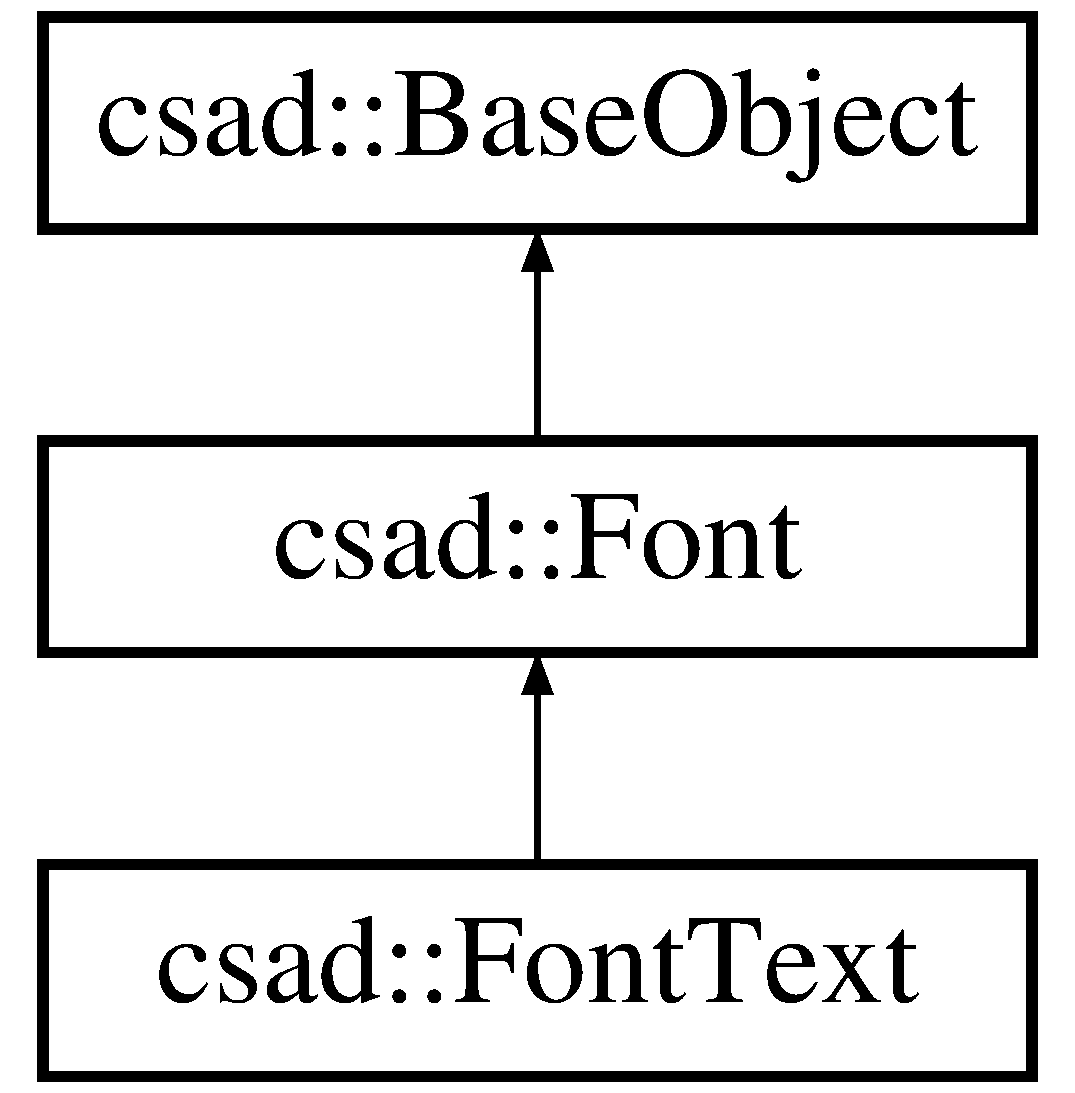
\includegraphics[height=3.000000cm]{classcsad_1_1_font}
\end{center}
\end{figure}
\subsection*{Public Types}
\begin{DoxyCompactItemize}
\item 
enum \hyperlink{classcsad_1_1_font_ae188d2f78967da23f4480c8c97ec7278}{Style} \{ \hyperlink{classcsad_1_1_font_ae188d2f78967da23f4480c8c97ec7278ab78e8c4ad9b4d68b50564b907448da6f}{N\-O\-N\-E} =0, 
\hyperlink{classcsad_1_1_font_ae188d2f78967da23f4480c8c97ec7278a78651b721318d08e8c454ce5163bb490}{B\-O\-L\-D} = 1, 
\hyperlink{classcsad_1_1_font_ae188d2f78967da23f4480c8c97ec7278ae0a0136bf3a895e6fd082a12aebc2976}{I\-T\-A\-L\-I\-C} = 2, 
\hyperlink{classcsad_1_1_font_ae188d2f78967da23f4480c8c97ec7278af4744703dcad7752115abee438ff4afb}{U\-N\-D\-E\-R\-L\-I\-N\-E} = 4
 \}
\begin{DoxyCompactList}\small\item\em font style, can mix \end{DoxyCompactList}\end{DoxyCompactItemize}
\subsection*{Public Member Functions}
\begin{DoxyCompactItemize}
\item 
\hypertarget{classcsad_1_1_font_a9d553674c4a9ef79bed298d6ce317c14}{virtual P\-L\-A\-T\-F\-O\-R\-M\-\_\-\-A\-P\-I float \hyperlink{classcsad_1_1_font_a9d553674c4a9ef79bed298d6ce317c14}{add\-Out\-Line} (int x, int y, char simvol, Geometry\-Path2\-I $\ast$path)}\label{classcsad_1_1_font_a9d553674c4a9ef79bed298d6ce317c14}

\begin{DoxyCompactList}\small\item\em Supplements geometry glyph of the specified character. \end{DoxyCompactList}\item 
\hypertarget{classcsad_1_1_font_ad97cd895f6afe64be19c7a9a18742347}{P\-L\-A\-T\-F\-O\-R\-M\-\_\-\-A\-P\-I const char $\ast$ \hyperlink{classcsad_1_1_font_ad97cd895f6afe64be19c7a9a18742347}{get\-Name} ()}\label{classcsad_1_1_font_ad97cd895f6afe64be19c7a9a18742347}

\begin{DoxyCompactList}\small\item\em return font name. \end{DoxyCompactList}\item 
\hypertarget{classcsad_1_1_font_a2630256d9732a3b47b0526d17f5748d7}{virtual P\-L\-A\-T\-F\-O\-R\-M\-\_\-\-A\-P\-I float \hyperlink{classcsad_1_1_font_a2630256d9732a3b47b0526d17f5748d7}{height} ()}\label{classcsad_1_1_font_a2630256d9732a3b47b0526d17f5748d7}

\begin{DoxyCompactList}\small\item\em font height \end{DoxyCompactList}\item 
\hypertarget{classcsad_1_1_font_a17a01ec3279f4504bac8885a7437fdfc}{virtual P\-L\-A\-T\-F\-O\-R\-M\-\_\-\-A\-P\-I void \hyperlink{classcsad_1_1_font_a17a01ec3279f4504bac8885a7437fdfc}{raster\-Text} (void $\ast$raster, int x, int y, unsigned int color, int mode, char $\ast$text)}\label{classcsad_1_1_font_a17a01ec3279f4504bac8885a7437fdfc}

\begin{DoxyCompactList}\small\item\em Creates a raster of the text. \end{DoxyCompactList}\item 
\hypertarget{classcsad_1_1_font_a1e72b3d9af1d21f0c5042bfc6edec66f}{P\-L\-A\-T\-F\-O\-R\-M\-\_\-\-A\-P\-I void $\ast$ \hyperlink{classcsad_1_1_font_a1e72b3d9af1d21f0c5042bfc6edec66f}{set} (unsigned \-\_\-int32 id, void $\ast$param)}\label{classcsad_1_1_font_a1e72b3d9af1d21f0c5042bfc6edec66f}

\begin{DoxyCompactList}\small\item\em used for any interface commands. \end{DoxyCompactList}\item 
\hypertarget{classcsad_1_1_font_a10c9c756fc9fa5956b9466c9c15e9d13}{P\-L\-A\-T\-F\-O\-R\-M\-\_\-\-A\-P\-I void \hyperlink{classcsad_1_1_font_a10c9c756fc9fa5956b9466c9c15e9d13}{set\-Bold} (bool val)}\label{classcsad_1_1_font_a10c9c756fc9fa5956b9466c9c15e9d13}

\begin{DoxyCompactList}\small\item\em Sets the font style bold. \end{DoxyCompactList}\item 
\hypertarget{classcsad_1_1_font_afb80f95ef52ae2d3f8ab5efd7e57006b}{P\-L\-A\-T\-F\-O\-R\-M\-\_\-\-A\-P\-I void \hyperlink{classcsad_1_1_font_afb80f95ef52ae2d3f8ab5efd7e57006b}{set\-Italic} (bool val)}\label{classcsad_1_1_font_afb80f95ef52ae2d3f8ab5efd7e57006b}

\begin{DoxyCompactList}\small\item\em Sets the font style inclined. \end{DoxyCompactList}\item 
\hypertarget{classcsad_1_1_font_a5e2ec165289b5e809936dde5d0913f16}{P\-L\-A\-T\-F\-O\-R\-M\-\_\-\-A\-P\-I void \hyperlink{classcsad_1_1_font_a5e2ec165289b5e809936dde5d0913f16}{set\-Name} (char $\ast$name)}\label{classcsad_1_1_font_a5e2ec165289b5e809936dde5d0913f16}

\begin{DoxyCompactList}\small\item\em Specifies the name of the font, for some platforms, you set the font file name. \end{DoxyCompactList}\item 
\hypertarget{classcsad_1_1_font_ac1e1cc4a00300465b733911acacbed65}{virtual P\-L\-A\-T\-F\-O\-R\-M\-\_\-\-A\-P\-I void \hyperlink{classcsad_1_1_font_ac1e1cc4a00300465b733911acacbed65}{set\-Size} (int size)}\label{classcsad_1_1_font_ac1e1cc4a00300465b733911acacbed65}

\begin{DoxyCompactList}\small\item\em specifies the font size \end{DoxyCompactList}\item 
\hypertarget{classcsad_1_1_font_a4ac8d96b47c91cf8edf047ddc819158b}{virtual P\-L\-A\-T\-F\-O\-R\-M\-\_\-\-A\-P\-I void \hyperlink{classcsad_1_1_font_a4ac8d96b47c91cf8edf047ddc819158b}{set\-Style} (int style)}\label{classcsad_1_1_font_a4ac8d96b47c91cf8edf047ddc819158b}

\begin{DoxyCompactList}\small\item\em Sets the style of the font. \end{DoxyCompactList}\item 
\hypertarget{classcsad_1_1_font_a5bf4543b059c48b60c4c9b18afe6d7ca}{P\-L\-A\-T\-F\-O\-R\-M\-\_\-\-A\-P\-I void \hyperlink{classcsad_1_1_font_a5bf4543b059c48b60c4c9b18afe6d7ca}{set\-Under\-Line} (bool val)}\label{classcsad_1_1_font_a5bf4543b059c48b60c4c9b18afe6d7ca}

\begin{DoxyCompactList}\small\item\em Sets the font style underlined. \end{DoxyCompactList}\item 
\hypertarget{classcsad_1_1_font_aef48acccbb1dbf8c0334107293840b10}{virtual P\-L\-A\-T\-F\-O\-R\-M\-\_\-\-A\-P\-I float \hyperlink{classcsad_1_1_font_aef48acccbb1dbf8c0334107293840b10}{width} (char $\ast$text)}\label{classcsad_1_1_font_aef48acccbb1dbf8c0334107293840b10}

\begin{DoxyCompactList}\small\item\em Long labels. \end{DoxyCompactList}\end{DoxyCompactItemize}


\subsection{Detailed Description}
\hyperlink{classcsad_1_1_font}{Font} -\/ The font object belongs to font server. 

\begin{DoxyVerb}  <Font name="name" font="font name" size="size font"/>
\end{DoxyVerb}
 \begin{DoxySeeAlso}{See Also}
\hyperlink{classcsad_1_1_font_server}{Font\-Server}, \hyperlink{group__platform}{csad\-: platform} 
\end{DoxySeeAlso}


\subsection{Member Enumeration Documentation}
\hypertarget{classcsad_1_1_font_ae188d2f78967da23f4480c8c97ec7278}{\index{csad\-::\-Font@{csad\-::\-Font}!Style@{Style}}
\index{Style@{Style}!csad::Font@{csad\-::\-Font}}
\subsubsection[{Style}]{\setlength{\rightskip}{0pt plus 5cm}enum {\bf csad\-::\-Font\-::\-Style}}}\label{classcsad_1_1_font_ae188d2f78967da23f4480c8c97ec7278}


font style, can mix 

\begin{Desc}
\item[Enumerator]\par
\begin{description}
\index{N\-O\-N\-E@{N\-O\-N\-E}!csad\-::\-Font@{csad\-::\-Font}}\index{csad\-::\-Font@{csad\-::\-Font}!N\-O\-N\-E@{N\-O\-N\-E}}\item[{\em 
\hypertarget{classcsad_1_1_font_ae188d2f78967da23f4480c8c97ec7278ab78e8c4ad9b4d68b50564b907448da6f}{N\-O\-N\-E}\label{classcsad_1_1_font_ae188d2f78967da23f4480c8c97ec7278ab78e8c4ad9b4d68b50564b907448da6f}
}]default \index{B\-O\-L\-D@{B\-O\-L\-D}!csad\-::\-Font@{csad\-::\-Font}}\index{csad\-::\-Font@{csad\-::\-Font}!B\-O\-L\-D@{B\-O\-L\-D}}\item[{\em 
\hypertarget{classcsad_1_1_font_ae188d2f78967da23f4480c8c97ec7278a78651b721318d08e8c454ce5163bb490}{B\-O\-L\-D}\label{classcsad_1_1_font_ae188d2f78967da23f4480c8c97ec7278a78651b721318d08e8c454ce5163bb490}
}]bold style \index{I\-T\-A\-L\-I\-C@{I\-T\-A\-L\-I\-C}!csad\-::\-Font@{csad\-::\-Font}}\index{csad\-::\-Font@{csad\-::\-Font}!I\-T\-A\-L\-I\-C@{I\-T\-A\-L\-I\-C}}\item[{\em 
\hypertarget{classcsad_1_1_font_ae188d2f78967da23f4480c8c97ec7278ae0a0136bf3a895e6fd082a12aebc2976}{I\-T\-A\-L\-I\-C}\label{classcsad_1_1_font_ae188d2f78967da23f4480c8c97ec7278ae0a0136bf3a895e6fd082a12aebc2976}
}]italic style \index{U\-N\-D\-E\-R\-L\-I\-N\-E@{U\-N\-D\-E\-R\-L\-I\-N\-E}!csad\-::\-Font@{csad\-::\-Font}}\index{csad\-::\-Font@{csad\-::\-Font}!U\-N\-D\-E\-R\-L\-I\-N\-E@{U\-N\-D\-E\-R\-L\-I\-N\-E}}\item[{\em 
\hypertarget{classcsad_1_1_font_ae188d2f78967da23f4480c8c97ec7278af4744703dcad7752115abee438ff4afb}{U\-N\-D\-E\-R\-L\-I\-N\-E}\label{classcsad_1_1_font_ae188d2f78967da23f4480c8c97ec7278af4744703dcad7752115abee438ff4afb}
}]underline style \end{description}
\end{Desc}

\hypertarget{classcsad_1_1_font_server}{\section{csad\-:\-:Font\-Server Class Reference}
\label{classcsad_1_1_font_server}\index{csad\-::\-Font\-Server@{csad\-::\-Font\-Server}}
}


\hyperlink{classcsad_1_1_font_server}{Font\-Server} -\/ font Manager.  


Inheritance diagram for csad\-:\-:Font\-Server\-:\begin{figure}[H]
\begin{center}
\leavevmode
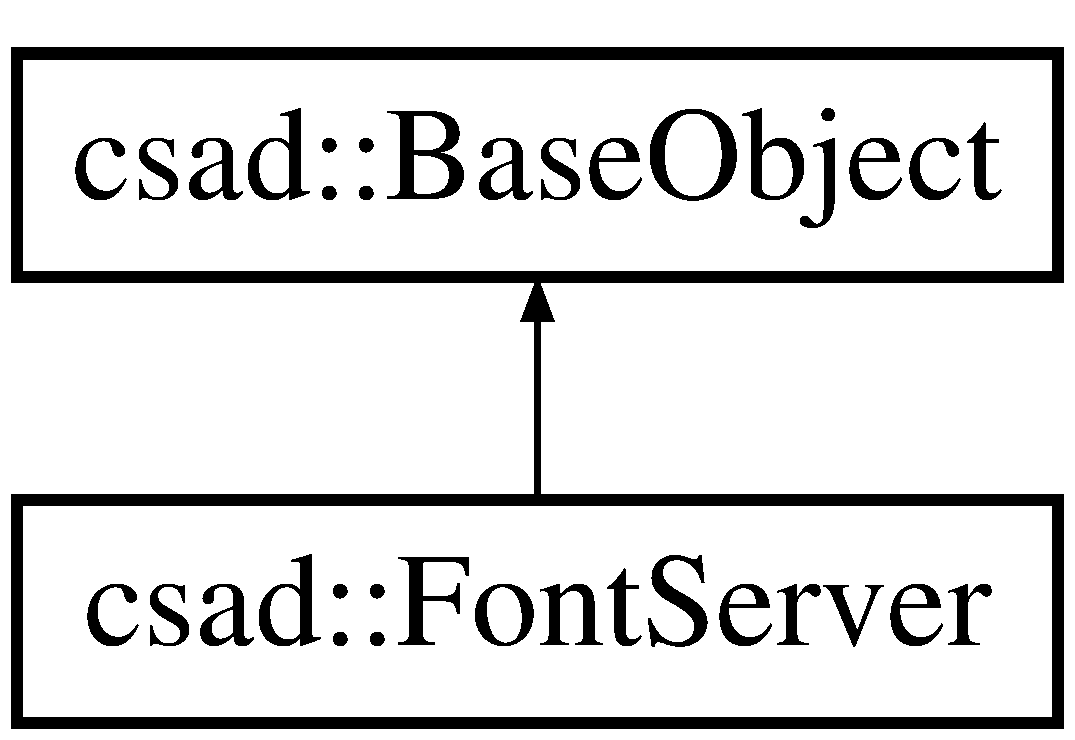
\includegraphics[height=2.000000cm]{classcsad_1_1_font_server}
\end{center}
\end{figure}
\subsection*{Public Member Functions}
\begin{DoxyCompactItemize}
\item 
\hypertarget{classcsad_1_1_font_server_a0dced757a18a02ea8c5894c9405e51b7}{P\-L\-A\-T\-F\-O\-R\-M\-\_\-\-A\-P\-I \hyperlink{classcsad_1_1_font}{Font} $\ast$ \hyperlink{classcsad_1_1_font_server_a0dced757a18a02ea8c5894c9405e51b7}{create\-Font} (char $\ast$name)}\label{classcsad_1_1_font_server_a0dced757a18a02ea8c5894c9405e51b7}

\begin{DoxyCompactList}\small\item\em Constructs a font by name. \end{DoxyCompactList}\item 
\hypertarget{classcsad_1_1_font_server_a63cb0951903f8e34302f443a011aabac}{P\-L\-A\-T\-F\-O\-R\-M\-\_\-\-A\-P\-I \hyperlink{classcsad_1_1_font_text}{Font\-Text} $\ast$ \hyperlink{classcsad_1_1_font_server_a63cb0951903f8e34302f443a011aabac}{create\-Font\-Text} (char $\ast$name)}\label{classcsad_1_1_font_server_a63cb0951903f8e34302f443a011aabac}

\begin{DoxyCompactList}\small\item\em Creates a texture font by name. \end{DoxyCompactList}\item 
\hypertarget{classcsad_1_1_font_server_a9a526980241ce80c3416295327c92b30}{P\-L\-A\-T\-F\-O\-R\-M\-\_\-\-A\-P\-I \hyperlink{classcsad_1_1_font}{Font} $\ast$ \hyperlink{classcsad_1_1_font_server_a9a526980241ce80c3416295327c92b30}{get\-Font} (char $\ast$name)}\label{classcsad_1_1_font_server_a9a526980241ce80c3416295327c92b30}

\begin{DoxyCompactList}\small\item\em Returns the font by name. \end{DoxyCompactList}\item 
\hypertarget{classcsad_1_1_font_server_a5ffcda094dc56c7ef068960bf6f03a04}{P\-L\-A\-T\-F\-O\-R\-M\-\_\-\-A\-P\-I \hyperlink{classcsad_1_1_font_text}{Font\-Text} $\ast$ \hyperlink{classcsad_1_1_font_server_a5ffcda094dc56c7ef068960bf6f03a04}{get\-Font\-Text} (char $\ast$name)}\label{classcsad_1_1_font_server_a5ffcda094dc56c7ef068960bf6f03a04}

\begin{DoxyCompactList}\small\item\em Returns the texture font by name. \end{DoxyCompactList}\item 
\hypertarget{classcsad_1_1_font_server_a34f907f08e1fd2dda02c1358590a1ffc}{P\-L\-A\-T\-F\-O\-R\-M\-\_\-\-A\-P\-I void $\ast$ \hyperlink{classcsad_1_1_font_server_a34f907f08e1fd2dda02c1358590a1ffc}{set} (unsigned \-\_\-int32, void $\ast$)}\label{classcsad_1_1_font_server_a34f907f08e1fd2dda02c1358590a1ffc}

\begin{DoxyCompactList}\small\item\em used for any interface commands. \end{DoxyCompactList}\end{DoxyCompactItemize}
\subsection*{Additional Inherited Members}


\subsection{Detailed Description}
\hyperlink{classcsad_1_1_font_server}{Font\-Server} -\/ font Manager. 

\begin{DoxyVerb}  <FontServer name="name" options="">
  ... Fonts ...
  </FontServer>
\end{DoxyVerb}


\begin{DoxySeeAlso}{See Also}
\hyperlink{classcsad_1_1_font_server}{Font\-Server}, \hyperlink{group__platform}{csad\-: platform} 
\end{DoxySeeAlso}

\hypertarget{classcsad_1_1_font_text}{\section{csad\-:\-:Font\-Text Class Reference}
\label{classcsad_1_1_font_text}\index{csad\-::\-Font\-Text@{csad\-::\-Font\-Text}}
}


\hyperlink{classcsad_1_1_font_text}{Font\-Text} -\/ Object bitmap texture font belongs to the font server.  


Inheritance diagram for csad\-:\-:Font\-Text\-:\begin{figure}[H]
\begin{center}
\leavevmode
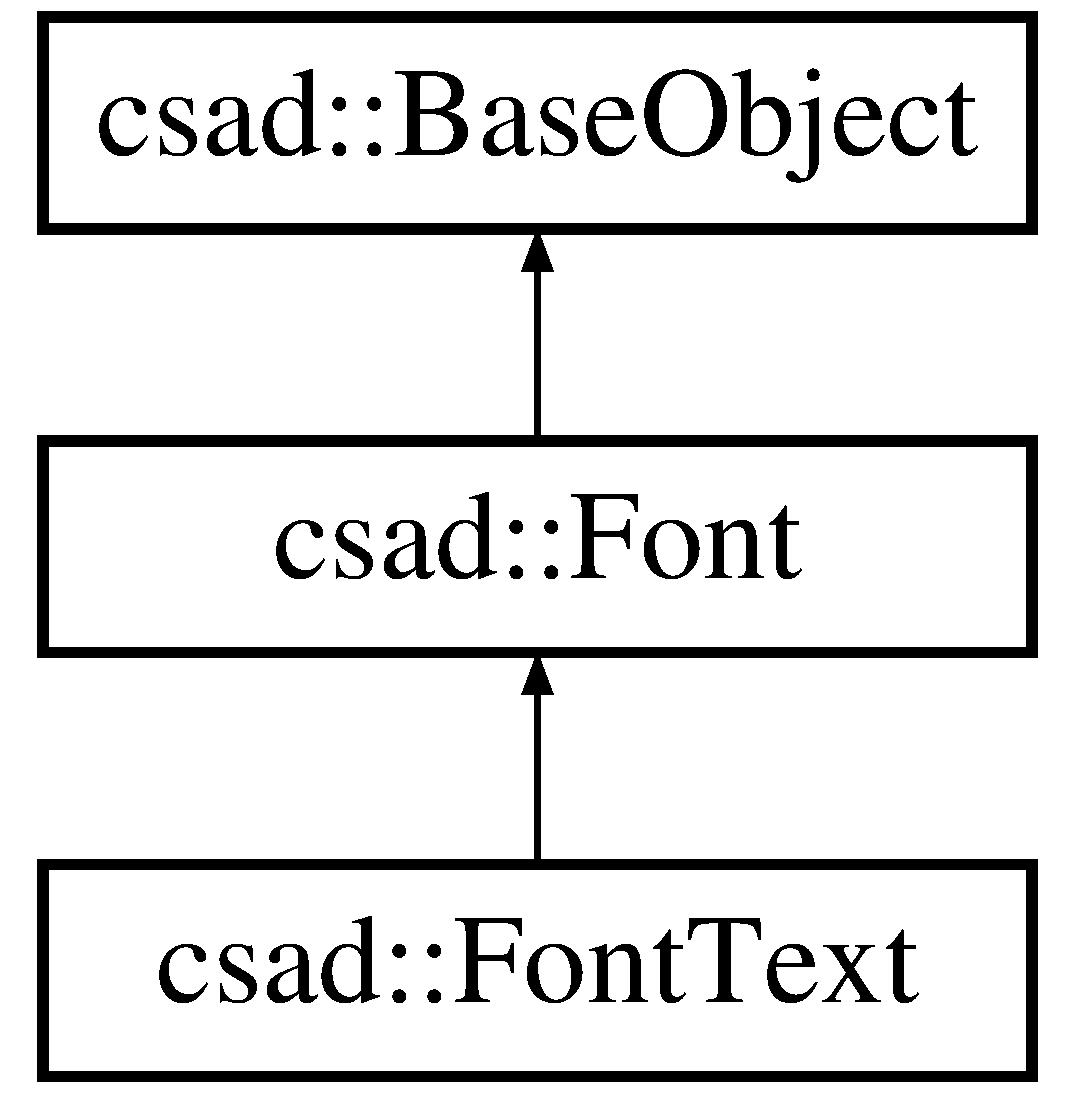
\includegraphics[height=3.000000cm]{classcsad_1_1_font_text}
\end{center}
\end{figure}
\subsection*{Public Member Functions}
\begin{DoxyCompactItemize}
\item 
\hypertarget{classcsad_1_1_font_text_a3a350fe5f637472c95e4641a0940ddf3}{C\-S\-A\-D\-\_\-\-A\-P\-I float \hyperlink{classcsad_1_1_font_text_a3a350fe5f637472c95e4641a0940ddf3}{height} ()}\label{classcsad_1_1_font_text_a3a350fe5f637472c95e4641a0940ddf3}

\begin{DoxyCompactList}\small\item\em font height \end{DoxyCompactList}\item 
\hypertarget{classcsad_1_1_font_text_ac8558fa7d3c70e813d9a9b85a91ecc17}{C\-S\-A\-D\-\_\-\-A\-P\-I void $\ast$ \hyperlink{classcsad_1_1_font_text_ac8558fa7d3c70e813d9a9b85a91ecc17}{set} (unsigned \-\_\-int32 id, void $\ast$param)}\label{classcsad_1_1_font_text_ac8558fa7d3c70e813d9a9b85a91ecc17}

\begin{DoxyCompactList}\small\item\em used for any interface commands. \end{DoxyCompactList}\item 
\hypertarget{classcsad_1_1_font_text_a159e2ef03c6f8189be9b2723e561659c}{C\-S\-A\-D\-\_\-\-A\-P\-I void \hyperlink{classcsad_1_1_font_text_a159e2ef03c6f8189be9b2723e561659c}{set\-Size} (int size)}\label{classcsad_1_1_font_text_a159e2ef03c6f8189be9b2723e561659c}

\begin{DoxyCompactList}\small\item\em specifies the font size \end{DoxyCompactList}\end{DoxyCompactItemize}
\subsection*{Additional Inherited Members}


\subsection{Detailed Description}
\hyperlink{classcsad_1_1_font_text}{Font\-Text} -\/ Object bitmap texture font belongs to the font server. 

\begin{DoxyVerb}  <FontText name="name" font="font name" size="size font"/>
\end{DoxyVerb}
 \begin{DoxySeeAlso}{See Also}
\hyperlink{classcsad_1_1_font}{Font}, \hyperlink{classcsad_1_1_font_server}{Font\-Server}, \hyperlink{group__platform}{csad\-: platform} 
\end{DoxySeeAlso}

\hypertarget{classcsad_1_1_format3_d_s}{\section{csad\-:\-:Format3\-D\-S Class Reference}
\label{classcsad_1_1_format3_d_s}\index{csad\-::\-Format3\-D\-S@{csad\-::\-Format3\-D\-S}}
}


\hyperlink{classcsad_1_1_format3_d_s}{Format3\-D\-S} -\/ файл экспортируемого формата 3\-D Studio Max.  




\subsection{Detailed Description}
\hyperlink{classcsad_1_1_format3_d_s}{Format3\-D\-S} -\/ файл экспортируемого формата 3\-D Studio Max. 

\begin{DoxySeeAlso}{See Also}
\hyperlink{group__format}{csad\-: format} 
\end{DoxySeeAlso}

\hypertarget{classcsad_1_1_format_j_p_g}{\section{csad\-:\-:Format\-J\-P\-G Class Reference}
\label{classcsad_1_1_format_j_p_g}\index{csad\-::\-Format\-J\-P\-G@{csad\-::\-Format\-J\-P\-G}}
}


\hyperlink{classcsad_1_1_format_j_p_g}{Format\-J\-P\-G} -\/ файл двухмерного изображения.  


\subsection*{Public Member Functions}
\begin{DoxyCompactItemize}
\item 
\hypertarget{classcsad_1_1_format_j_p_g_ad79274615ffe7197681de1f7d74ab679}{\-\_\-\-F\-O\-R\-C\-E\-I\-N\-L\-I\-N\-E int \hyperlink{classcsad_1_1_format_j_p_g_ad79274615ffe7197681de1f7d74ab679}{bpp} ()}\label{classcsad_1_1_format_j_p_g_ad79274615ffe7197681de1f7d74ab679}

\begin{DoxyCompactList}\small\item\em возвращает количество байт на пиксей \end{DoxyCompactList}\item 
\hypertarget{classcsad_1_1_format_j_p_g_a4c805cd9aa25a3356d45e0844a1eeadd}{C\-S\-A\-D\-\_\-\-A\-P\-I void \hyperlink{classcsad_1_1_format_j_p_g_a4c805cd9aa25a3356d45e0844a1eeadd}{clear} ()}\label{classcsad_1_1_format_j_p_g_a4c805cd9aa25a3356d45e0844a1eeadd}

\begin{DoxyCompactList}\small\item\em очистка от всех данных \end{DoxyCompactList}\item 
\hypertarget{classcsad_1_1_format_j_p_g_a126275f7c14f4a00733b19aace6338d0}{\-\_\-\-F\-O\-R\-C\-E\-I\-N\-L\-I\-N\-E int \hyperlink{classcsad_1_1_format_j_p_g_a126275f7c14f4a00733b19aace6338d0}{height} ()}\label{classcsad_1_1_format_j_p_g_a126275f7c14f4a00733b19aace6338d0}

\begin{DoxyCompactList}\small\item\em высота цветовой матирци. \end{DoxyCompactList}\item 
\hypertarget{classcsad_1_1_format_j_p_g_a824d4ca3a31fc557b463a5781c560496}{\-\_\-\-F\-O\-R\-C\-E\-I\-N\-L\-I\-N\-E void $\ast$ \hyperlink{classcsad_1_1_format_j_p_g_a824d4ca3a31fc557b463a5781c560496}{img\-Matrix} ()}\label{classcsad_1_1_format_j_p_g_a824d4ca3a31fc557b463a5781c560496}

\begin{DoxyCompactList}\small\item\em возвращает указатель на двухмерную цветовую матрицу \end{DoxyCompactList}\item 
\hypertarget{classcsad_1_1_format_j_p_g_a1a6d6fdeed54dfe07d3d230bced2c1f6}{C\-S\-A\-D\-\_\-\-A\-P\-I bool \hyperlink{classcsad_1_1_format_j_p_g_a1a6d6fdeed54dfe07d3d230bced2c1f6}{read\-From\-File} (char $\ast$name)}\label{classcsad_1_1_format_j_p_g_a1a6d6fdeed54dfe07d3d230bced2c1f6}

\begin{DoxyCompactList}\small\item\em Загружает и декодирует файл. \end{DoxyCompactList}\item 
\hypertarget{classcsad_1_1_format_j_p_g_a3f24728b4fbae6a6fbc9ed0631c318fe}{\-\_\-\-F\-O\-R\-C\-E\-I\-N\-L\-I\-N\-E bool \hyperlink{classcsad_1_1_format_j_p_g_a3f24728b4fbae6a6fbc9ed0631c318fe}{read\-From\-File} (const char $\ast$name)}\label{classcsad_1_1_format_j_p_g_a3f24728b4fbae6a6fbc9ed0631c318fe}

\begin{DoxyCompactList}\small\item\em Загружает и декодирует файл. \end{DoxyCompactList}\item 
\hypertarget{classcsad_1_1_format_j_p_g_a85348c86c213591aca70fcabf263b28a}{C\-S\-A\-D\-\_\-\-A\-P\-I bool \hyperlink{classcsad_1_1_format_j_p_g_a85348c86c213591aca70fcabf263b28a}{read\-From\-File} (\hyperlink{classcsad_1_1_file}{File} $\ast$file)}\label{classcsad_1_1_format_j_p_g_a85348c86c213591aca70fcabf263b28a}

\begin{DoxyCompactList}\small\item\em Загружает и декодирует файл. \end{DoxyCompactList}\item 
\hypertarget{classcsad_1_1_format_j_p_g_aaff0ede2ca4dcd16b0f97ca92700cfa9}{\-\_\-\-F\-O\-R\-C\-E\-I\-N\-L\-I\-N\-E void \hyperlink{classcsad_1_1_format_j_p_g_aaff0ede2ca4dcd16b0f97ca92700cfa9}{set\-Matrix} (void $\ast$data)}\label{classcsad_1_1_format_j_p_g_aaff0ede2ca4dcd16b0f97ca92700cfa9}

\begin{DoxyCompactList}\small\item\em задает цветовую матрицу для текущего формата \end{DoxyCompactList}\item 
\hypertarget{classcsad_1_1_format_j_p_g_ae18001750b21ddaff6d05a52a146ff08}{C\-S\-A\-D\-\_\-\-A\-P\-I void \hyperlink{classcsad_1_1_format_j_p_g_ae18001750b21ddaff6d05a52a146ff08}{set\-Matrix} (int \hyperlink{classcsad_1_1_format_j_p_g_a126275f7c14f4a00733b19aace6338d0}{height}, int \hyperlink{classcsad_1_1_format_j_p_g_a1a3684e2216ec08fee5d016bf3a12338}{width}, int \hyperlink{classcsad_1_1_format_j_p_g_ad79274615ffe7197681de1f7d74ab679}{bpp}, void $\ast$data)}\label{classcsad_1_1_format_j_p_g_ae18001750b21ddaff6d05a52a146ff08}

\begin{DoxyCompactList}\small\item\em задает цветовую матрицу и ее формат \end{DoxyCompactList}\item 
\hypertarget{classcsad_1_1_format_j_p_g_a1a3684e2216ec08fee5d016bf3a12338}{\-\_\-\-F\-O\-R\-C\-E\-I\-N\-L\-I\-N\-E int \hyperlink{classcsad_1_1_format_j_p_g_a1a3684e2216ec08fee5d016bf3a12338}{width} ()}\label{classcsad_1_1_format_j_p_g_a1a3684e2216ec08fee5d016bf3a12338}

\begin{DoxyCompactList}\small\item\em ширина цветовой матирци. \end{DoxyCompactList}\end{DoxyCompactItemize}


\subsection{Detailed Description}
\hyperlink{classcsad_1_1_format_j_p_g}{Format\-J\-P\-G} -\/ файл двухмерного изображения. 

\begin{DoxySeeAlso}{See Also}
\hyperlink{group__format}{csad\-: format} 
\end{DoxySeeAlso}

\hypertarget{classcsad_1_1_format_p_a_k}{\section{csad\-:\-:Format\-P\-A\-K Class Reference}
\label{classcsad_1_1_format_p_a_k}\index{csad\-::\-Format\-P\-A\-K@{csad\-::\-Format\-P\-A\-K}}
}


\hyperlink{classcsad_1_1_format_p_a_k}{Format\-P\-A\-K} -\/ файл контейнер.  




\subsection{Detailed Description}
\hyperlink{classcsad_1_1_format_p_a_k}{Format\-P\-A\-K} -\/ файл контейнер. 

\begin{DoxySeeAlso}{See Also}
\hyperlink{group__format}{csad\-: format} 
\end{DoxySeeAlso}

\hypertarget{classcsad_1_1_format_t_g_a}{\section{csad\-:\-:Format\-T\-G\-A Class Reference}
\label{classcsad_1_1_format_t_g_a}\index{csad\-::\-Format\-T\-G\-A@{csad\-::\-Format\-T\-G\-A}}
}


\hyperlink{classcsad_1_1_format_t_g_a}{Format\-T\-G\-A} -\/ файл двухмерного изображения.  


\subsection*{Public Member Functions}
\begin{DoxyCompactItemize}
\item 
\hypertarget{classcsad_1_1_format_t_g_a_a92c9f8db7378a2dd4968bfdc7713729c}{\-\_\-\-F\-O\-R\-C\-E\-I\-N\-L\-I\-N\-E int \hyperlink{classcsad_1_1_format_t_g_a_a92c9f8db7378a2dd4968bfdc7713729c}{bpp} ()}\label{classcsad_1_1_format_t_g_a_a92c9f8db7378a2dd4968bfdc7713729c}

\begin{DoxyCompactList}\small\item\em возвращает количество байт на пиксей \end{DoxyCompactList}\item 
\hypertarget{classcsad_1_1_format_t_g_a_a8306c75bcd5965aa66240b7af2e40d11}{\-\_\-\-F\-O\-R\-C\-E\-I\-N\-L\-I\-N\-E int \hyperlink{classcsad_1_1_format_t_g_a_a8306c75bcd5965aa66240b7af2e40d11}{height} ()}\label{classcsad_1_1_format_t_g_a_a8306c75bcd5965aa66240b7af2e40d11}

\begin{DoxyCompactList}\small\item\em высота цветовой матирци. \end{DoxyCompactList}\item 
\hypertarget{classcsad_1_1_format_t_g_a_acebaababf481d1b48b6f63af59c95632}{\-\_\-\-F\-O\-R\-C\-E\-I\-N\-L\-I\-N\-E void $\ast$ \hyperlink{classcsad_1_1_format_t_g_a_acebaababf481d1b48b6f63af59c95632}{img\-Matrix} ()}\label{classcsad_1_1_format_t_g_a_acebaababf481d1b48b6f63af59c95632}

\begin{DoxyCompactList}\small\item\em возвращает указатель на двухмерную цветовую матрицу \end{DoxyCompactList}\item 
\hypertarget{classcsad_1_1_format_t_g_a_ab2eda94d067cb4dd7dbfef17f9eba359}{C\-S\-A\-D\-\_\-\-A\-P\-I bool \hyperlink{classcsad_1_1_format_t_g_a_ab2eda94d067cb4dd7dbfef17f9eba359}{read\-From\-File} (char $\ast$name)}\label{classcsad_1_1_format_t_g_a_ab2eda94d067cb4dd7dbfef17f9eba359}

\begin{DoxyCompactList}\small\item\em Загружает и декодирует файл. \end{DoxyCompactList}\item 
\hypertarget{classcsad_1_1_format_t_g_a_a62b2c3c00b00b90aa8f88b0f503a6be3}{\-\_\-\-F\-O\-R\-C\-E\-I\-N\-L\-I\-N\-E bool \hyperlink{classcsad_1_1_format_t_g_a_a62b2c3c00b00b90aa8f88b0f503a6be3}{read\-From\-File} (const char $\ast$name)}\label{classcsad_1_1_format_t_g_a_a62b2c3c00b00b90aa8f88b0f503a6be3}

\begin{DoxyCompactList}\small\item\em Загружает и декодирует файл. \end{DoxyCompactList}\item 
\hypertarget{classcsad_1_1_format_t_g_a_a76b4094f054b922ce42ddf0dadc5e32c}{C\-S\-A\-D\-\_\-\-A\-P\-I bool \hyperlink{classcsad_1_1_format_t_g_a_a76b4094f054b922ce42ddf0dadc5e32c}{read\-From\-File} (\hyperlink{classcsad_1_1_file}{File} $\ast$file)}\label{classcsad_1_1_format_t_g_a_a76b4094f054b922ce42ddf0dadc5e32c}

\begin{DoxyCompactList}\small\item\em Загружает и декодирует файл. \end{DoxyCompactList}\item 
\hypertarget{classcsad_1_1_format_t_g_a_a81605ff0a5fbf281117efcf250a1e54b}{\-\_\-\-F\-O\-R\-C\-E\-I\-N\-L\-I\-N\-E void \hyperlink{classcsad_1_1_format_t_g_a_a81605ff0a5fbf281117efcf250a1e54b}{set\-Matrix} (void $\ast$data)}\label{classcsad_1_1_format_t_g_a_a81605ff0a5fbf281117efcf250a1e54b}

\begin{DoxyCompactList}\small\item\em задает цветовую матрицу для текущего формата \end{DoxyCompactList}\end{DoxyCompactItemize}


\subsection{Detailed Description}
\hyperlink{classcsad_1_1_format_t_g_a}{Format\-T\-G\-A} -\/ файл двухмерного изображения. 

\begin{DoxySeeAlso}{See Also}
\hyperlink{group__format}{csad\-: format} 
\end{DoxySeeAlso}

\hypertarget{classcsad_1_1_format_x_m_l}{\section{csad\-:\-:Format\-X\-M\-L Class Reference}
\label{classcsad_1_1_format_x_m_l}\index{csad\-::\-Format\-X\-M\-L@{csad\-::\-Format\-X\-M\-L}}
}


\hyperlink{classcsad_1_1_format_x_m_l}{Format\-X\-M\-L} -\/ the format of the xml data file.  


\subsection*{Public Member Functions}
\begin{DoxyCompactItemize}
\item 
\hypertarget{classcsad_1_1_format_x_m_l_a1aa09f102b7ea207089af1f678eb8122}{\-\_\-\-F\-O\-R\-C\-E\-I\-N\-L\-I\-N\-E \hyperlink{classcsad_1_1_node_x_m_l}{Node\-X\-M\-L} $\ast$ \hyperlink{classcsad_1_1_format_x_m_l_a1aa09f102b7ea207089af1f678eb8122}{get\-Node} ()}\label{classcsad_1_1_format_x_m_l_a1aa09f102b7ea207089af1f678eb8122}

\begin{DoxyCompactList}\small\item\em returns the root element \end{DoxyCompactList}\item 
C\-S\-A\-D\-\_\-\-A\-P\-I \hyperlink{classcsad_1_1_node_x_m_l}{Node\-X\-M\-L} $\ast$ \hyperlink{classcsad_1_1_format_x_m_l_a9899ec63a8c33281011f711f0b0ce6ff}{get\-Node\-By\-Path} (char $\ast$path)
\item 
\hypertarget{classcsad_1_1_format_x_m_l_a3356445cf390e438136a51d8cf47b6f2}{C\-S\-A\-D\-\_\-\-A\-P\-I \hyperlink{classcsad_1_1_node_x_m_l}{Node\-X\-M\-L} $\ast$ \hyperlink{classcsad_1_1_format_x_m_l_a3356445cf390e438136a51d8cf47b6f2}{new\-Node} (\hyperlink{classcsad_1_1_node_x_m_l}{Node\-X\-M\-L} $\ast$parent)}\label{classcsad_1_1_format_x_m_l_a3356445cf390e438136a51d8cf47b6f2}

\begin{DoxyCompactList}\small\item\em Creates a node from a specified parent or root node. \end{DoxyCompactList}\item 
\hypertarget{classcsad_1_1_format_x_m_l_a22e3a24dc005675c38ea237114bc0538}{C\-S\-A\-D\-\_\-\-A\-P\-I bool \hyperlink{classcsad_1_1_format_x_m_l_a22e3a24dc005675c38ea237114bc0538}{read\-From\-File} (char $\ast$name)}\label{classcsad_1_1_format_x_m_l_a22e3a24dc005675c38ea237114bc0538}

\begin{DoxyCompactList}\small\item\em Loading from a file at the specified path. \end{DoxyCompactList}\item 
\hypertarget{classcsad_1_1_format_x_m_l_ab02214b17baf6d4dcdd2a4621dd9cf29}{C\-S\-A\-D\-\_\-\-A\-P\-I bool \hyperlink{classcsad_1_1_format_x_m_l_ab02214b17baf6d4dcdd2a4621dd9cf29}{read\-From\-File} (\hyperlink{classcsad_1_1_file}{File} $\ast$file)}\label{classcsad_1_1_format_x_m_l_ab02214b17baf6d4dcdd2a4621dd9cf29}

\begin{DoxyCompactList}\small\item\em Загрузка из файла \end{DoxyCompactList}\item 
\hypertarget{classcsad_1_1_format_x_m_l_a8da41425b3b61fe1b68b3455fc0a6b8f}{C\-S\-A\-D\-\_\-\-A\-P\-I bool \hyperlink{classcsad_1_1_format_x_m_l_a8da41425b3b61fe1b68b3455fc0a6b8f}{save\-To\-File} (char $\ast$name)}\label{classcsad_1_1_format_x_m_l_a8da41425b3b61fe1b68b3455fc0a6b8f}

\begin{DoxyCompactList}\small\item\em Write to the file at the specified path. \end{DoxyCompactList}\item 
\hypertarget{classcsad_1_1_format_x_m_l_a978030ec8cb813ef6f9505febbc3596d}{C\-S\-A\-D\-\_\-\-A\-P\-I bool \hyperlink{classcsad_1_1_format_x_m_l_a978030ec8cb813ef6f9505febbc3596d}{save\-To\-File} (\hyperlink{classcsad_1_1_file}{File} $\ast$file)}\label{classcsad_1_1_format_x_m_l_a978030ec8cb813ef6f9505febbc3596d}

\begin{DoxyCompactList}\small\item\em Запись в файл \end{DoxyCompactList}\end{DoxyCompactItemize}


\subsection{Detailed Description}
\hyperlink{classcsad_1_1_format_x_m_l}{Format\-X\-M\-L} -\/ the format of the xml data file. 

The object containing the X\-M\-L hierarchy Tagoo, starting from the virtual root element with the name of the file.

\begin{DoxySeeAlso}{See Also}
\hyperlink{group__format}{csad\-: format} 
\end{DoxySeeAlso}


\subsection{Member Function Documentation}
\hypertarget{classcsad_1_1_format_x_m_l_a9899ec63a8c33281011f711f0b0ce6ff}{\index{csad\-::\-Format\-X\-M\-L@{csad\-::\-Format\-X\-M\-L}!get\-Node\-By\-Path@{get\-Node\-By\-Path}}
\index{get\-Node\-By\-Path@{get\-Node\-By\-Path}!csad::FormatXML@{csad\-::\-Format\-X\-M\-L}}
\subsubsection[{get\-Node\-By\-Path}]{\setlength{\rightskip}{0pt plus 5cm}C\-S\-A\-D\-\_\-\-A\-P\-I {\bf Node\-X\-M\-L}$\ast$ csad\-::\-Format\-X\-M\-L\-::get\-Node\-By\-Path (
\begin{DoxyParamCaption}
\item[{char $\ast$}]{path}
\end{DoxyParamCaption}
)}}\label{classcsad_1_1_format_x_m_l_a9899ec63a8c33281011f711f0b0ce6ff}
returns the node for submission 
\begin{DoxyParams}{Parameters}
{\em path} & -\/ the path of hierarchie \char`\"{}first/second\mbox{[}3\mbox{]}/param\mbox{[}2\mbox{]}\char`\"{} \\
\hline
\end{DoxyParams}

\hypertarget{classcsad_1_1_gl_context}{\section{csad\-:\-:Gl\-Context Class Reference}
\label{classcsad_1_1_gl_context}\index{csad\-::\-Gl\-Context@{csad\-::\-Gl\-Context}}
}


\hyperlink{classcsad_1_1_gl_context}{Gl\-Context} -\/ the context interface Open\-G\-L/\-Open\-G\-L\-E\-S.  


Inheritance diagram for csad\-:\-:Gl\-Context\-:\begin{figure}[H]
\begin{center}
\leavevmode
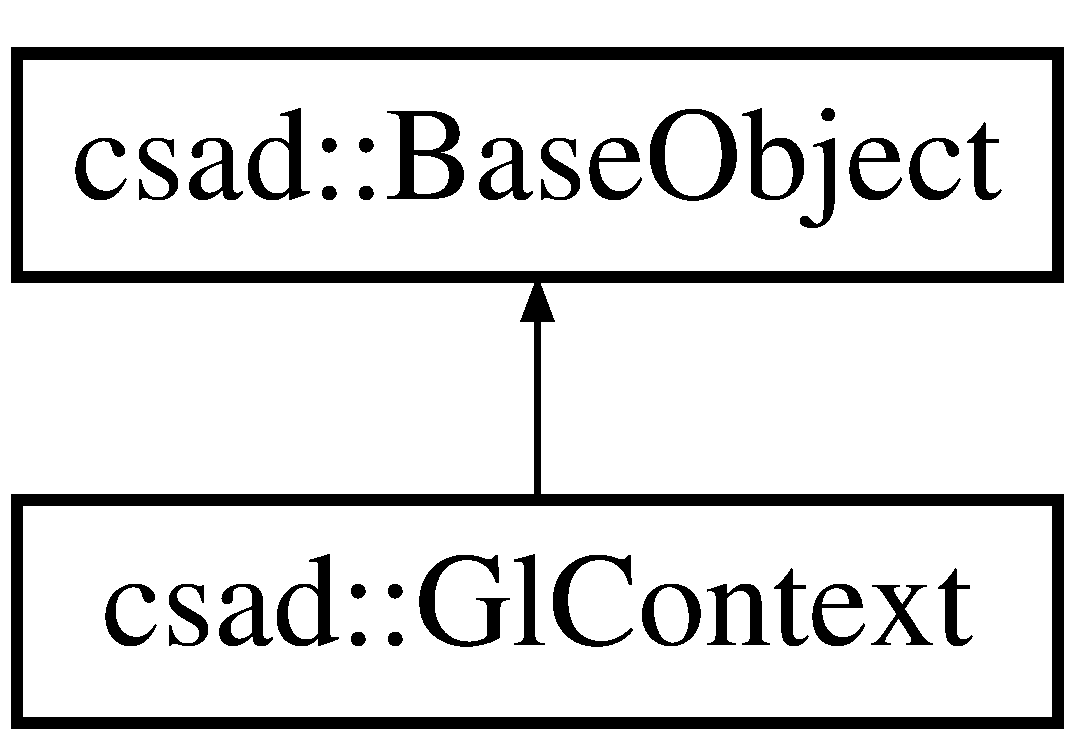
\includegraphics[height=2.000000cm]{classcsad_1_1_gl_context}
\end{center}
\end{figure}
\subsection*{Public Member Functions}
\begin{DoxyCompactItemize}
\item 
\hypertarget{classcsad_1_1_gl_context_a523a508de3ed4f0181f682b271f54707}{P\-L\-A\-T\-F\-O\-R\-M\-\_\-\-A\-P\-I unsigned int \hyperlink{classcsad_1_1_gl_context_a523a508de3ed4f0181f682b271f54707}{create\-Texture2\-D} ()}\label{classcsad_1_1_gl_context_a523a508de3ed4f0181f682b271f54707}

\begin{DoxyCompactList}\small\item\em Creates a new texture devices. \end{DoxyCompactList}\item 
\hypertarget{classcsad_1_1_gl_context_a74578d0e8d3e9bb788c9ac4f0f3883f0}{\-\_\-\-F\-O\-R\-C\-E\-I\-N\-L\-I\-N\-E \hyperlink{classcsad_1_1_display}{Display} $\ast$ \hyperlink{classcsad_1_1_gl_context_a74578d0e8d3e9bb788c9ac4f0f3883f0}{get\-Display} ()}\label{classcsad_1_1_gl_context_a74578d0e8d3e9bb788c9ac4f0f3883f0}

\begin{DoxyCompactList}\small\item\em Returns the parent device. \end{DoxyCompactList}\item 
\hypertarget{classcsad_1_1_gl_context_a2c2b7ecefc48c082981b562e4b0ac991}{P\-L\-A\-T\-F\-O\-R\-M\-\_\-\-A\-P\-I int \hyperlink{classcsad_1_1_gl_context_a2c2b7ecefc48c082981b562e4b0ac991}{height} ()}\label{classcsad_1_1_gl_context_a2c2b7ecefc48c082981b562e4b0ac991}

\begin{DoxyCompactList}\small\item\em Returns the height of the screen. \end{DoxyCompactList}\item 
\hypertarget{classcsad_1_1_gl_context_a2e6b41f9ad9bf94c19248eef33e7a8cf}{P\-L\-A\-T\-F\-O\-R\-M\-\_\-\-A\-P\-I bool \hyperlink{classcsad_1_1_gl_context_a2e6b41f9ad9bf94c19248eef33e7a8cf}{make\-Current} ()}\label{classcsad_1_1_gl_context_a2e6b41f9ad9bf94c19248eef33e7a8cf}

\begin{DoxyCompactList}\small\item\em Activates the context. \end{DoxyCompactList}\item 
\hypertarget{classcsad_1_1_gl_context_a1104b694664c559ed5ec6595a2cff327}{P\-L\-A\-T\-F\-O\-R\-M\-\_\-\-A\-P\-I void $\ast$ \hyperlink{classcsad_1_1_gl_context_a1104b694664c559ed5ec6595a2cff327}{set} (unsigned \-\_\-int32, void $\ast$)}\label{classcsad_1_1_gl_context_a1104b694664c559ed5ec6595a2cff327}

\begin{DoxyCompactList}\small\item\em used for any interface commands. \end{DoxyCompactList}\item 
\hypertarget{classcsad_1_1_gl_context_a72ef9a9feddc9265b5175b6dacb249ae}{P\-L\-A\-T\-F\-O\-R\-M\-\_\-\-A\-P\-I int \hyperlink{classcsad_1_1_gl_context_a72ef9a9feddc9265b5175b6dacb249ae}{width} ()}\label{classcsad_1_1_gl_context_a72ef9a9feddc9265b5175b6dacb249ae}

\begin{DoxyCompactList}\small\item\em Returns the width of the screen. \end{DoxyCompactList}\end{DoxyCompactItemize}
\subsection*{Static Public Member Functions}
\begin{DoxyCompactItemize}
\item 
\hypertarget{classcsad_1_1_gl_context_a01e495e2d572ec32282abc324a3373bb}{static P\-L\-A\-T\-F\-O\-R\-M\-\_\-\-A\-P\-I \hyperlink{classcsad_1_1_gl_context}{Gl\-Context} $\ast$ \hyperlink{classcsad_1_1_gl_context_a01e495e2d572ec32282abc324a3373bb}{get\-Current} ()}\label{classcsad_1_1_gl_context_a01e495e2d572ec32282abc324a3373bb}

\begin{DoxyCompactList}\small\item\em Returns the active context. \end{DoxyCompactList}\end{DoxyCompactItemize}
\subsection*{Additional Inherited Members}


\subsection{Detailed Description}
\hyperlink{classcsad_1_1_gl_context}{Gl\-Context} -\/ the context interface Open\-G\-L/\-Open\-G\-L\-E\-S. 

\begin{DoxyVerb}  <Display name="display name">
     <GlContext name="context name" />
  </Display>
\end{DoxyVerb}


\begin{DoxySeeAlso}{See Also}
\hyperlink{group__core}{csad\-: core} 
\end{DoxySeeAlso}

\hypertarget{classcsad_1_1_graph}{\section{csad\-:\-:Graph Class Reference}
\label{classcsad_1_1_graph}\index{csad\-::\-Graph@{csad\-::\-Graph}}
}


\hyperlink{classcsad_1_1_graph}{Graph} -\/ Manager graphics.  


Inheritance diagram for csad\-:\-:Graph\-:\begin{figure}[H]
\begin{center}
\leavevmode
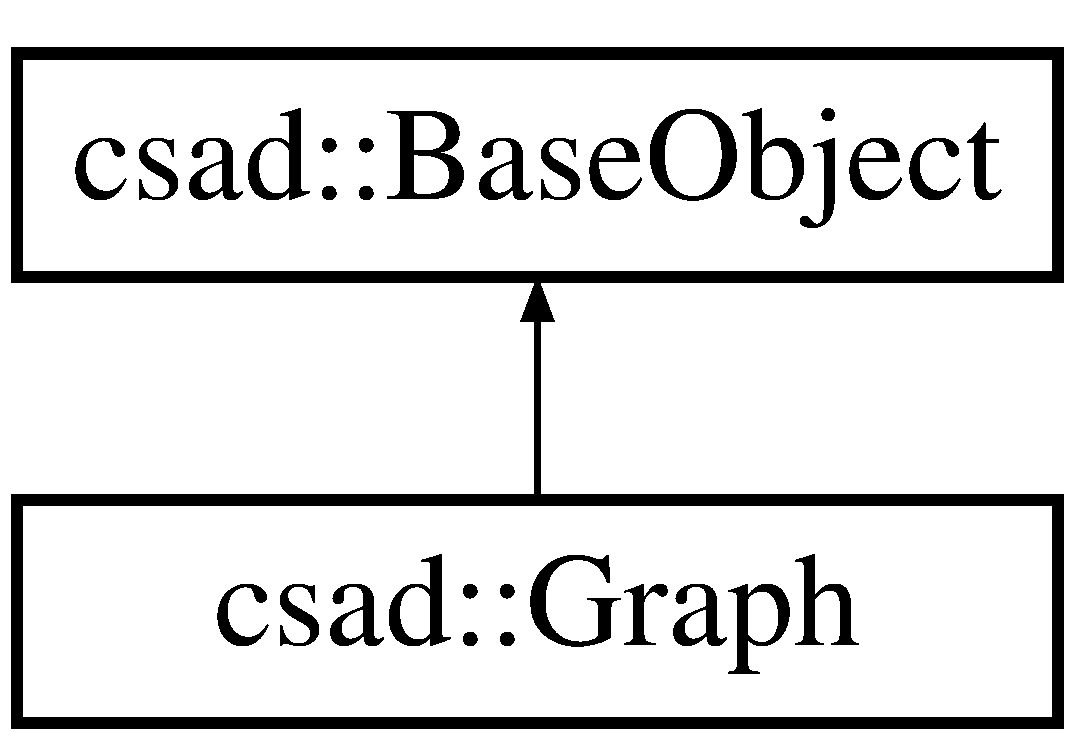
\includegraphics[height=2.000000cm]{classcsad_1_1_graph}
\end{center}
\end{figure}
\subsection*{Public Member Functions}
\begin{DoxyCompactItemize}
\item 
\hypertarget{classcsad_1_1_graph_a53bc5a6d553e4381bc642719322a6cb5}{C\-S\-A\-D\-\_\-\-A\-P\-I \hyperlink{classcsad_1_1_display}{Display} $\ast$ \hyperlink{classcsad_1_1_graph_a53bc5a6d553e4381bc642719322a6cb5}{create\-Display} (char $\ast$name)}\label{classcsad_1_1_graph_a53bc5a6d553e4381bc642719322a6cb5}

\begin{DoxyCompactList}\small\item\em Creates the object of the screen with the specified name, or returns available if the object of the screen with the same name already been created. \end{DoxyCompactList}\item 
\hypertarget{classcsad_1_1_graph_af95625ac8e2b5327901f632554c985a3}{C\-S\-A\-D\-\_\-\-A\-P\-I \hyperlink{classcsad_1_1_material}{Material} $\ast$ \hyperlink{classcsad_1_1_graph_af95625ac8e2b5327901f632554c985a3}{create\-Material} (char $\ast$name)}\label{classcsad_1_1_graph_af95625ac8e2b5327901f632554c985a3}

\begin{DoxyCompactList}\small\item\em Creates material. \end{DoxyCompactList}\item 
\hypertarget{classcsad_1_1_graph_a074f1bbd06340c3d880bd4912d4a3e08}{\-\_\-\-F\-O\-R\-C\-E\-I\-N\-L\-I\-N\-E \hyperlink{classcsad_1_1_material}{Material} $\ast$ \hyperlink{classcsad_1_1_graph_a074f1bbd06340c3d880bd4912d4a3e08}{create\-Material} (const char $\ast$name=\char`\"{}\char`\"{})}\label{classcsad_1_1_graph_a074f1bbd06340c3d880bd4912d4a3e08}

\begin{DoxyCompactList}\small\item\em Creates material. \end{DoxyCompactList}\item 
\hypertarget{classcsad_1_1_graph_a3192d7f765642798d9e1bc16e7438b4a}{C\-S\-A\-D\-\_\-\-A\-P\-I \hyperlink{classcsad_1_1_scene}{Scene} $\ast$ \hyperlink{classcsad_1_1_graph_a3192d7f765642798d9e1bc16e7438b4a}{create\-Scene} (char $\ast$name)}\label{classcsad_1_1_graph_a3192d7f765642798d9e1bc16e7438b4a}

\begin{DoxyCompactList}\small\item\em Creates the environment of the scene with the specified name, or returns available if the environment of the scene with the same name already been created. \end{DoxyCompactList}\item 
\hypertarget{classcsad_1_1_graph_a064c03e4562046ada26844c7ec885aaa}{\-\_\-\-F\-O\-R\-C\-E\-I\-N\-L\-I\-N\-E \hyperlink{classcsad_1_1_scene}{Scene} $\ast$ \hyperlink{classcsad_1_1_graph_a064c03e4562046ada26844c7ec885aaa}{create\-Scene} (const char $\ast$name=\char`\"{}\char`\"{})}\label{classcsad_1_1_graph_a064c03e4562046ada26844c7ec885aaa}

\begin{DoxyCompactList}\small\item\em Creates the environment of the scene with the specified name, or returns available if the environment of the scene with the same name already been created. \end{DoxyCompactList}\item 
\hypertarget{classcsad_1_1_graph_a032c241f5e9fca9315d1d48460182a39}{C\-S\-A\-D\-\_\-\-A\-P\-I \hyperlink{classcsad_1_1_shader}{Shader} $\ast$ \hyperlink{classcsad_1_1_graph_a032c241f5e9fca9315d1d48460182a39}{create\-Shader} (char $\ast$name)}\label{classcsad_1_1_graph_a032c241f5e9fca9315d1d48460182a39}

\begin{DoxyCompactList}\small\item\em Creates \hyperlink{classcsad_1_1_shader}{Shader}. \end{DoxyCompactList}\item 
\hypertarget{classcsad_1_1_graph_a8d47d1485e3976eefe0724e252ed0de2}{\-\_\-\-F\-O\-R\-C\-E\-I\-N\-L\-I\-N\-E \hyperlink{classcsad_1_1_shader}{Shader} $\ast$ \hyperlink{classcsad_1_1_graph_a8d47d1485e3976eefe0724e252ed0de2}{create\-Shader} (const char $\ast$name=\char`\"{}\char`\"{})}\label{classcsad_1_1_graph_a8d47d1485e3976eefe0724e252ed0de2}

\begin{DoxyCompactList}\small\item\em Creates \hyperlink{classcsad_1_1_shader}{Shader}. \end{DoxyCompactList}\item 
\hypertarget{classcsad_1_1_graph_a680f5cf5bf6c4c4a79557a660a9f1e7d}{C\-S\-A\-D\-\_\-\-A\-P\-I \hyperlink{classcsad_1_1_style}{Style} $\ast$ \hyperlink{classcsad_1_1_graph_a680f5cf5bf6c4c4a79557a660a9f1e7d}{create\-Style} (char $\ast$name)}\label{classcsad_1_1_graph_a680f5cf5bf6c4c4a79557a660a9f1e7d}

\begin{DoxyCompactList}\small\item\em Creates a container styles, or returns available if the container styles with the same name already been created. \end{DoxyCompactList}\item 
\hypertarget{classcsad_1_1_graph_adda94dd62ffc4aa808634bfca84dc25b}{\-\_\-\-F\-O\-R\-C\-E\-I\-N\-L\-I\-N\-E \hyperlink{classcsad_1_1_style}{Style} $\ast$ \hyperlink{classcsad_1_1_graph_adda94dd62ffc4aa808634bfca84dc25b}{create\-Style} (const char $\ast$name=\char`\"{}\char`\"{})}\label{classcsad_1_1_graph_adda94dd62ffc4aa808634bfca84dc25b}

\begin{DoxyCompactList}\small\item\em Creates a container styles, or returns available if the container styles with the same name already been created. \end{DoxyCompactList}\item 
\hypertarget{classcsad_1_1_graph_a6de282f17fe6762354212b5d932b4d71}{C\-S\-A\-D\-\_\-\-A\-P\-I \hyperlink{classcsad_1_1_texture2_d}{Texture2\-D} $\ast$ \hyperlink{classcsad_1_1_graph_a6de282f17fe6762354212b5d932b4d71}{create\-Texture2\-D} (char $\ast$name)}\label{classcsad_1_1_graph_a6de282f17fe6762354212b5d932b4d71}

\begin{DoxyCompactList}\small\item\em Creates texture. \end{DoxyCompactList}\item 
\hypertarget{classcsad_1_1_graph_a53ec7bff2d2881675f0c934eebc66b1e}{C\-S\-A\-D\-\_\-\-A\-P\-I \hyperlink{classcsad_1_1_gl_context}{Gl\-Context} $\ast$ \hyperlink{classcsad_1_1_graph_a53ec7bff2d2881675f0c934eebc66b1e}{get\-Context} (char $\ast$path)}\label{classcsad_1_1_graph_a53ec7bff2d2881675f0c934eebc66b1e}

\begin{DoxyCompactList}\small\item\em returns the object context in his way \end{DoxyCompactList}\item 
\hypertarget{classcsad_1_1_graph_a4937813c5fdb26dc12ca1360344a28ce}{C\-S\-A\-D\-\_\-\-A\-P\-I \hyperlink{classcsad_1_1_display}{Display} $\ast$ \hyperlink{classcsad_1_1_graph_a4937813c5fdb26dc12ca1360344a28ce}{get\-Display} (char $\ast$name)}\label{classcsad_1_1_graph_a4937813c5fdb26dc12ca1360344a28ce}

\begin{DoxyCompactList}\small\item\em Restores a screen object at the specified name. \end{DoxyCompactList}\item 
\hypertarget{classcsad_1_1_graph_a9b483cf1f8583362b672813375527e10}{C\-S\-A\-D\-\_\-\-A\-P\-I \hyperlink{classcsad_1_1_display}{Display} $\ast$ \hyperlink{classcsad_1_1_graph_a9b483cf1f8583362b672813375527e10}{get\-Display\-By\-Handle} (void $\ast$handle)}\label{classcsad_1_1_graph_a9b483cf1f8583362b672813375527e10}

\begin{DoxyCompactList}\small\item\em Restores a screen object associated with the specified I\-D image. \end{DoxyCompactList}\item 
\hypertarget{classcsad_1_1_graph_a6487e2fab26cf007688b3e990aa925a7}{C\-S\-A\-D\-\_\-\-A\-P\-I \hyperlink{classcsad_1_1_display}{Display} $\ast$ \hyperlink{classcsad_1_1_graph_a6487e2fab26cf007688b3e990aa925a7}{get\-Display\-Intersect} (\hyperlink{classbt_1_1vector3f}{vector3f} $\ast$pos)}\label{classcsad_1_1_graph_a6487e2fab26cf007688b3e990aa925a7}

\begin{DoxyCompactList}\small\item\em Restores a screen object associated with the specified point. \end{DoxyCompactList}\item 
\hypertarget{classcsad_1_1_graph_a34762d6962ec058d36d9f9dde42c9a37}{C\-S\-A\-D\-\_\-\-A\-P\-I \hyperlink{classcsad_1_1_material}{Material} $\ast$ \hyperlink{classcsad_1_1_graph_a34762d6962ec058d36d9f9dde42c9a37}{get\-Material} (char $\ast$name)}\label{classcsad_1_1_graph_a34762d6962ec058d36d9f9dde42c9a37}

\begin{DoxyCompactList}\small\item\em returns the мaterial object by its name \end{DoxyCompactList}\item 
\hypertarget{classcsad_1_1_graph_a4d0c84d3e29c452fffc84d2979c8b274}{\-\_\-\-F\-O\-R\-C\-E\-I\-N\-L\-I\-N\-E \hyperlink{classcsad_1_1_material}{Material} $\ast$ \hyperlink{classcsad_1_1_graph_a4d0c84d3e29c452fffc84d2979c8b274}{get\-Material} (const char $\ast$name)}\label{classcsad_1_1_graph_a4d0c84d3e29c452fffc84d2979c8b274}

\begin{DoxyCompactList}\small\item\em returns the мaterial object by its name \end{DoxyCompactList}\item 
\hypertarget{classcsad_1_1_graph_abaa187b0797ea4adfbdb10384f98c57c}{C\-S\-A\-D\-\_\-\-A\-P\-I \hyperlink{classcsad_1_1_scene}{Scene} $\ast$ \hyperlink{classcsad_1_1_graph_abaa187b0797ea4adfbdb10384f98c57c}{get\-Scene} (char $\ast$name)}\label{classcsad_1_1_graph_abaa187b0797ea4adfbdb10384f98c57c}

\begin{DoxyCompactList}\small\item\em Returns the scene with the specified name. \end{DoxyCompactList}\item 
\hypertarget{classcsad_1_1_graph_ab59e8d239ebfb02c3324f4444c524b21}{C\-S\-A\-D\-\_\-\-A\-P\-I \hyperlink{classcsad_1_1_shader}{Shader} $\ast$ \hyperlink{classcsad_1_1_graph_ab59e8d239ebfb02c3324f4444c524b21}{get\-Shader} (char $\ast$name)}\label{classcsad_1_1_graph_ab59e8d239ebfb02c3324f4444c524b21}

\begin{DoxyCompactList}\small\item\em returns the texture object by its name \end{DoxyCompactList}\item 
\hypertarget{classcsad_1_1_graph_acc31c77a666e7d69e67ae87ba4096d5f}{\-\_\-\-F\-O\-R\-C\-E\-I\-N\-L\-I\-N\-E \hyperlink{classcsad_1_1_shader}{Shader} $\ast$ \hyperlink{classcsad_1_1_graph_acc31c77a666e7d69e67ae87ba4096d5f}{get\-Shader} (const char $\ast$name)}\label{classcsad_1_1_graph_acc31c77a666e7d69e67ae87ba4096d5f}

\begin{DoxyCompactList}\small\item\em returns the texture object by its name \end{DoxyCompactList}\item 
\hypertarget{classcsad_1_1_graph_ab692b69f2cc4bf190371f43fd22fe711}{C\-S\-A\-D\-\_\-\-A\-P\-I \hyperlink{classcsad_1_1_style}{Style} $\ast$ \hyperlink{classcsad_1_1_graph_ab692b69f2cc4bf190371f43fd22fe711}{get\-Style} (char $\ast$name)}\label{classcsad_1_1_graph_ab692b69f2cc4bf190371f43fd22fe711}

\begin{DoxyCompactList}\small\item\em returns the container style object by its name \end{DoxyCompactList}\item 
\hypertarget{classcsad_1_1_graph_a4bbdc58c479f9e69d77da5d796b9c021}{\-\_\-\-F\-O\-R\-C\-E\-I\-N\-L\-I\-N\-E \hyperlink{classcsad_1_1_style}{Style} $\ast$ \hyperlink{classcsad_1_1_graph_a4bbdc58c479f9e69d77da5d796b9c021}{get\-Style} (const char $\ast$name)}\label{classcsad_1_1_graph_a4bbdc58c479f9e69d77da5d796b9c021}

\begin{DoxyCompactList}\small\item\em returns the container style object by its name \end{DoxyCompactList}\item 
\hypertarget{classcsad_1_1_graph_a329447b6cb22fda4b6c2b3cea3fcaeb5}{C\-S\-A\-D\-\_\-\-A\-P\-I \hyperlink{classcsad_1_1_texture2_d}{Texture2\-D} $\ast$ \hyperlink{classcsad_1_1_graph_a329447b6cb22fda4b6c2b3cea3fcaeb5}{get\-Texture2\-D} (char $\ast$name)}\label{classcsad_1_1_graph_a329447b6cb22fda4b6c2b3cea3fcaeb5}

\begin{DoxyCompactList}\small\item\em returns the texture object by its name \end{DoxyCompactList}\item 
\hypertarget{classcsad_1_1_graph_a18ecc20248ea21c84fa82cb4cdb1d259}{\-\_\-\-F\-O\-R\-C\-E\-I\-N\-L\-I\-N\-E \hyperlink{classcsad_1_1_texture2_d}{Texture2\-D} $\ast$ \hyperlink{classcsad_1_1_graph_a18ecc20248ea21c84fa82cb4cdb1d259}{get\-Texture2\-D} (const char $\ast$name)}\label{classcsad_1_1_graph_a18ecc20248ea21c84fa82cb4cdb1d259}

\begin{DoxyCompactList}\small\item\em returns the texture object by its name \end{DoxyCompactList}\item 
\hypertarget{classcsad_1_1_graph_a8581c2147ae1f11eaae62e491139c367}{C\-S\-A\-D\-\_\-\-A\-P\-I void $\ast$ \hyperlink{classcsad_1_1_graph_a8581c2147ae1f11eaae62e491139c367}{set} (unsigned \-\_\-int32, void $\ast$)}\label{classcsad_1_1_graph_a8581c2147ae1f11eaae62e491139c367}

\begin{DoxyCompactList}\small\item\em used for any interface commands. \end{DoxyCompactList}\end{DoxyCompactItemize}
\subsection*{Static Public Member Functions}
\begin{DoxyCompactItemize}
\item 
\hypertarget{classcsad_1_1_graph_a7f35986797f46f1d7b9f02aaec278ee8}{static C\-S\-A\-D\-\_\-\-A\-P\-I \hyperlink{classcsad_1_1_graph}{Graph} \& \hyperlink{classcsad_1_1_graph_a7f35986797f46f1d7b9f02aaec278ee8}{graph} ()}\label{classcsad_1_1_graph_a7f35986797f46f1d7b9f02aaec278ee8}

\begin{DoxyCompactList}\small\item\em Active Manager graphical elements. \end{DoxyCompactList}\item 
\hypertarget{classcsad_1_1_graph_ad14c015d4c5b3f2dd101851a50ae2e08}{static C\-S\-A\-D\-\_\-\-A\-P\-I \hyperlink{classcsad_1_1_scene}{Scene} $\ast$ \hyperlink{classcsad_1_1_graph_ad14c015d4c5b3f2dd101851a50ae2e08}{scene} ()}\label{classcsad_1_1_graph_ad14c015d4c5b3f2dd101851a50ae2e08}

\begin{DoxyCompactList}\small\item\em active scene, the scene becomes active during the build its projection using \hyperlink{classcsad_1_1_renderer}{Renderer} \end{DoxyCompactList}\item 
\hypertarget{classcsad_1_1_graph_ac988039675f40f70ca7910adf993c3df}{static C\-S\-A\-D\-\_\-\-A\-P\-I bool \hyperlink{classcsad_1_1_graph_ac988039675f40f70ca7910adf993c3df}{type} (void $\ast$type)}\label{classcsad_1_1_graph_ac988039675f40f70ca7910adf993c3df}

\begin{DoxyCompactList}\small\item\em returns true if the object type belongs to the graphics Manager \end{DoxyCompactList}\end{DoxyCompactItemize}
\subsection*{Additional Inherited Members}


\subsection{Detailed Description}
\hyperlink{classcsad_1_1_graph}{Graph} -\/ Manager graphics. 

\begin{DoxySeeAlso}{See Also}
\hyperlink{group__core}{csad\-: core} 
\end{DoxySeeAlso}

\hypertarget{classcsad_1_1_input}{\section{csad\-:\-:Input Class Reference}
\label{classcsad_1_1_input}\index{csad\-::\-Input@{csad\-::\-Input}}
}


\hyperlink{classcsad_1_1_input}{Input} -\/ Manager device input.  


Inheritance diagram for csad\-:\-:Input\-:\begin{figure}[H]
\begin{center}
\leavevmode
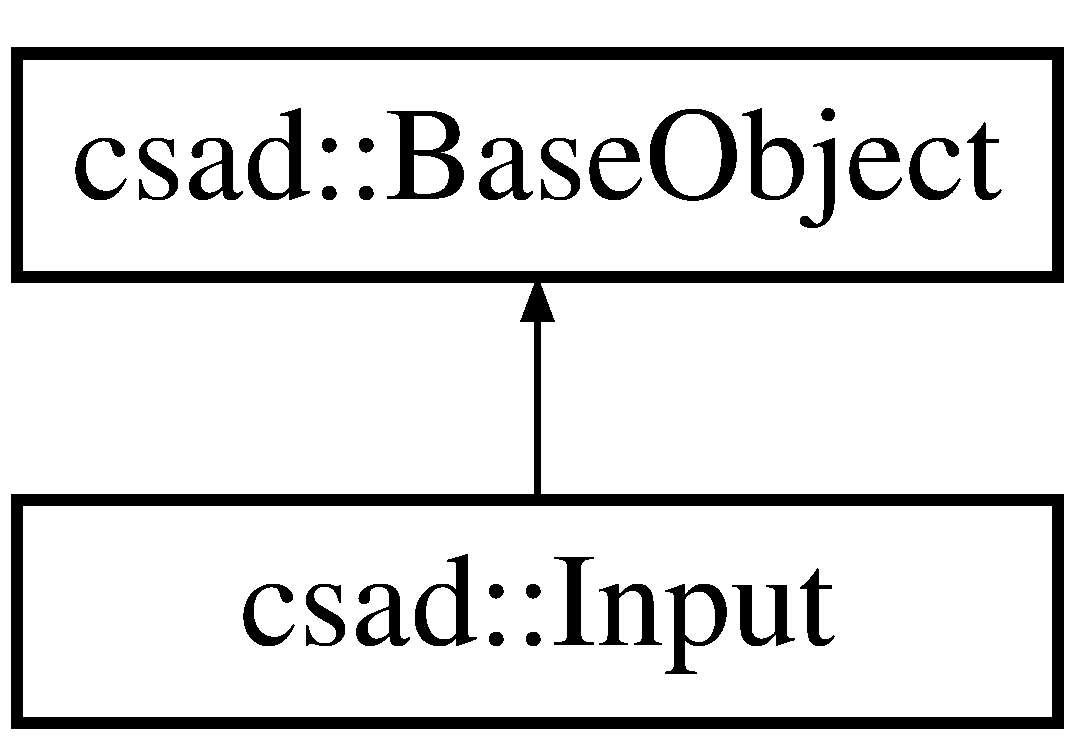
\includegraphics[height=2.000000cm]{classcsad_1_1_input}
\end{center}
\end{figure}
\subsection*{Public Member Functions}
\begin{DoxyCompactItemize}
\item 
\hypertarget{classcsad_1_1_input_a757f75633c889167613ca0e9d3f3b3ae}{C\-S\-A\-D\-\_\-\-A\-P\-I void \hyperlink{classcsad_1_1_input_a757f75633c889167613ca0e9d3f3b3ae}{close} ()}\label{classcsad_1_1_input_a757f75633c889167613ca0e9d3f3b3ae}

\begin{DoxyCompactList}\small\item\em the event handler \end{DoxyCompactList}\item 
\hypertarget{classcsad_1_1_input_a66e7b00df0774d9f9992dd527d9f804b}{C\-S\-A\-D\-\_\-\-A\-P\-I \hyperlink{classcsad_1_1_keyboard}{Keyboard} $\ast$ \hyperlink{classcsad_1_1_input_a66e7b00df0774d9f9992dd527d9f804b}{create\-Keyboard} (char $\ast$driver, char $\ast$name)}\label{classcsad_1_1_input_a66e7b00df0774d9f9992dd527d9f804b}

\begin{DoxyCompactList}\small\item\em creates an event handler for an input device type keyboard \end{DoxyCompactList}\item 
\hypertarget{classcsad_1_1_input_a152ed3adbe69cc7c6198c8a4fba0929a}{C\-S\-A\-D\-\_\-\-A\-P\-I \hyperlink{classcsad_1_1_mouse}{Mouse} $\ast$ \hyperlink{classcsad_1_1_input_a152ed3adbe69cc7c6198c8a4fba0929a}{create\-Mouse} (char $\ast$driver, char $\ast$name)}\label{classcsad_1_1_input_a152ed3adbe69cc7c6198c8a4fba0929a}

\begin{DoxyCompactList}\small\item\em creates an event handler for an input device type mouse \end{DoxyCompactList}\item 
\hypertarget{classcsad_1_1_input_a2f469ce209550a6dc86f91193fa78d5d}{\-\_\-\-F\-O\-R\-C\-E\-I\-N\-L\-I\-N\-E bool \hyperlink{classcsad_1_1_input_a2f469ce209550a6dc86f91193fa78d5d}{get\-Button} (unsigned int id)}\label{classcsad_1_1_input_a2f469ce209550a6dc86f91193fa78d5d}

\begin{DoxyCompactList}\small\item\em Returns the status of the specified key. \end{DoxyCompactList}\item 
\hypertarget{classcsad_1_1_input_a766f390a9baa2e03d487724d72904551}{\-\_\-\-F\-O\-R\-C\-E\-I\-N\-L\-I\-N\-E \hyperlink{classbt_1_1vector3f}{vector3f} \& \hyperlink{classcsad_1_1_input_a766f390a9baa2e03d487724d72904551}{get\-Cursor\-Delta} ()}\label{classcsad_1_1_input_a766f390a9baa2e03d487724d72904551}

\begin{DoxyCompactList}\small\item\em The offset of the General provisions of the cursor all manipulators. \end{DoxyCompactList}\item 
\hypertarget{classcsad_1_1_input_a1afaf2cf308eb0da1c7ca06b713d375b}{\-\_\-\-F\-O\-R\-C\-E\-I\-N\-L\-I\-N\-E \hyperlink{classbt_1_1vector3f}{vector3f} \& \hyperlink{classcsad_1_1_input_a1afaf2cf308eb0da1c7ca06b713d375b}{get\-Cursor\-Pos} ()}\label{classcsad_1_1_input_a1afaf2cf308eb0da1c7ca06b713d375b}

\begin{DoxyCompactList}\small\item\em The General position of the cursor all manipulators. \end{DoxyCompactList}\item 
\hypertarget{classcsad_1_1_input_a0acafcd1d8b3ed76d8abbfbfc12de84d}{\-\_\-\-F\-O\-R\-C\-E\-I\-N\-L\-I\-N\-E \hyperlink{classcsad_1_1_display}{Display} $\ast$ \hyperlink{classcsad_1_1_input_a0acafcd1d8b3ed76d8abbfbfc12de84d}{get\-Display} ()}\label{classcsad_1_1_input_a0acafcd1d8b3ed76d8abbfbfc12de84d}

\begin{DoxyCompactList}\small\item\em The screen on which the mouse is. \end{DoxyCompactList}\item 
\hypertarget{classcsad_1_1_input_a24d54b9c326d129e45c780e1b52b6205}{C\-S\-A\-D\-\_\-\-A\-P\-I \hyperlink{classcsad_1_1_keyboard}{Keyboard} $\ast$ \hyperlink{classcsad_1_1_input_a24d54b9c326d129e45c780e1b52b6205}{get\-Keyboard} (char $\ast$name)}\label{classcsad_1_1_input_a24d54b9c326d129e45c780e1b52b6205}

\begin{DoxyCompactList}\small\item\em Returns an object keyboard. \end{DoxyCompactList}\item 
\hypertarget{classcsad_1_1_input_a0d7ef03bb02cb17f0bf0f745f9e367bc}{C\-S\-A\-D\-\_\-\-A\-P\-I \hyperlink{classcsad_1_1_mouse}{Mouse} $\ast$ \hyperlink{classcsad_1_1_input_a0d7ef03bb02cb17f0bf0f745f9e367bc}{get\-Mouse} (char $\ast$name)}\label{classcsad_1_1_input_a0d7ef03bb02cb17f0bf0f745f9e367bc}

\begin{DoxyCompactList}\small\item\em Returns an object of a mouse. \end{DoxyCompactList}\item 
\hypertarget{classcsad_1_1_input_a41d9e739c64e71760fc3bf079ca752c7}{C\-S\-A\-D\-\_\-\-A\-P\-I T\-Y\-P\-E\-I\-N\-F\-O\-\_\-\-H C\-S\-A\-D\-\_\-\-A\-P\-I void \hyperlink{classcsad_1_1_input_a41d9e739c64e71760fc3bf079ca752c7}{init} ()}\label{classcsad_1_1_input_a41d9e739c64e71760fc3bf079ca752c7}

\begin{DoxyCompactList}\small\item\em the event handler \end{DoxyCompactList}\item 
\hypertarget{classcsad_1_1_input_ae88db6f7b3d9498032f34a3a5f1f121c}{C\-S\-A\-D\-\_\-\-A\-P\-I void $\ast$ \hyperlink{classcsad_1_1_input_ae88db6f7b3d9498032f34a3a5f1f121c}{set} (unsigned \-\_\-int32, void $\ast$)}\label{classcsad_1_1_input_ae88db6f7b3d9498032f34a3a5f1f121c}

\begin{DoxyCompactList}\small\item\em used for any interface commands. \end{DoxyCompactList}\item 
\hypertarget{classcsad_1_1_input_a81bc6c33ac661fac050f8e7447921b43}{C\-S\-A\-D\-\_\-\-A\-P\-I void \hyperlink{classcsad_1_1_input_a81bc6c33ac661fac050f8e7447921b43}{update} ()}\label{classcsad_1_1_input_a81bc6c33ac661fac050f8e7447921b43}

\begin{DoxyCompactList}\small\item\em the event handler \end{DoxyCompactList}\item 
\hypertarget{classcsad_1_1_input_a6ac63c7befd7af801d8bdac4a7379639}{C\-S\-A\-D\-\_\-\-A\-P\-I void \hyperlink{classcsad_1_1_input_a6ac63c7befd7af801d8bdac4a7379639}{update\-Reset} ()}\label{classcsad_1_1_input_a6ac63c7befd7af801d8bdac4a7379639}

\begin{DoxyCompactList}\small\item\em the event handler \end{DoxyCompactList}\end{DoxyCompactItemize}
\subsection*{Static Public Member Functions}
\begin{DoxyCompactItemize}
\item 
\hypertarget{classcsad_1_1_input_a2e64e6fdc610c1e20ff299ae73b965a3}{static C\-S\-A\-D\-\_\-\-A\-P\-I \hyperlink{classcsad_1_1_input}{Input} \& \hyperlink{classcsad_1_1_input_a2e64e6fdc610c1e20ff299ae73b965a3}{input} ()}\label{classcsad_1_1_input_a2e64e6fdc610c1e20ff299ae73b965a3}

\begin{DoxyCompactList}\small\item\em Provides access to the active input Manager. \end{DoxyCompactList}\end{DoxyCompactItemize}
\subsection*{Additional Inherited Members}


\subsection{Detailed Description}
\hyperlink{classcsad_1_1_input}{Input} -\/ Manager device input. 

\begin{DoxySeeAlso}{See Also}
\hyperlink{classcsad_1_1_input_a2e64e6fdc610c1e20ff299ae73b965a3}{input} 
\end{DoxySeeAlso}

\hypertarget{classcsad_1_1_interface_data_system}{\section{csad\-:\-:Interface\-Data\-System Class Reference}
\label{classcsad_1_1_interface_data_system}\index{csad\-::\-Interface\-Data\-System@{csad\-::\-Interface\-Data\-System}}
}


\hyperlink{classcsad_1_1_interface_data_system}{Interface\-Data\-System} -\/ system data manager.  


\subsection*{Public Member Functions}
\begin{DoxyCompactItemize}
\item 
\hypertarget{classcsad_1_1_interface_data_system_a237a7ec3260d3fb4d67937e4eb940767}{C\-S\-A\-D\-\_\-\-A\-P\-I void \hyperlink{classcsad_1_1_interface_data_system_a237a7ec3260d3fb4d67937e4eb940767}{load\-Raster} (char $\ast$filename, gen\-::\-Raster $\ast$$\ast$raster)}\label{classcsad_1_1_interface_data_system_a237a7ec3260d3fb4d67937e4eb940767}

\begin{DoxyCompactList}\small\item\em отложенная загрузка ресурса двухмерного изображеня \end{DoxyCompactList}\item 
\hypertarget{classcsad_1_1_interface_data_system_a310d28ddebd9041062fdeed896426cfb}{C\-S\-A\-D\-\_\-\-A\-P\-I void \hyperlink{classcsad_1_1_interface_data_system_a310d28ddebd9041062fdeed896426cfb}{load\-Raster\-To\-Texture2\-D} (char $\ast$filename, \hyperlink{classcsad_1_1_texture2_d}{Texture2\-D} $\ast$text)}\label{classcsad_1_1_interface_data_system_a310d28ddebd9041062fdeed896426cfb}

\begin{DoxyCompactList}\small\item\em отложенная загрузка ресурса двухмерного изображеня в текстуру \end{DoxyCompactList}\end{DoxyCompactItemize}


\subsection{Detailed Description}
\hyperlink{classcsad_1_1_interface_data_system}{Interface\-Data\-System} -\/ system data manager. 

\begin{DoxySeeAlso}{See Also}
\hyperlink{group__core}{csad\-: core} 
\end{DoxySeeAlso}

\hypertarget{classcsad_1_1_keyboard}{\section{csad\-:\-:Keyboard Class Reference}
\label{classcsad_1_1_keyboard}\index{csad\-::\-Keyboard@{csad\-::\-Keyboard}}
}


\hyperlink{classcsad_1_1_keyboard}{Keyboard} -\/ the object input system, platform dependent.  




Inherits csad\-::\-Base\-Keyboard.

\subsection*{Public Member Functions}
\begin{DoxyCompactItemize}
\item 
\hypertarget{classcsad_1_1_keyboard_a71846e6913baa68e34d5b7024b2e6683}{C\-S\-A\-D\-\_\-\-A\-P\-I bool \hyperlink{classcsad_1_1_keyboard_a71846e6913baa68e34d5b7024b2e6683}{get\-Key} (int id)}\label{classcsad_1_1_keyboard_a71846e6913baa68e34d5b7024b2e6683}

\begin{DoxyCompactList}\small\item\em Return if key pressed;. \end{DoxyCompactList}\item 
\hypertarget{classcsad_1_1_keyboard_aae4475094b70b614bb5acde35dfaf65e}{C\-S\-A\-D\-\_\-\-A\-P\-I char $\ast$ \hyperlink{classcsad_1_1_keyboard_aae4475094b70b614bb5acde35dfaf65e}{get\-Map} ()}\label{classcsad_1_1_keyboard_aae4475094b70b614bb5acde35dfaf65e}

\begin{DoxyCompactList}\small\item\em Return array of bits keys;. \end{DoxyCompactList}\item 
\hypertarget{classcsad_1_1_keyboard_a192d3a7516da6ca21d3ebe82a6b2507c}{C\-S\-A\-D\-\_\-\-A\-P\-I void $\ast$ \hyperlink{classcsad_1_1_keyboard_a192d3a7516da6ca21d3ebe82a6b2507c}{set} (unsigned \-\_\-int32, void $\ast$)}\label{classcsad_1_1_keyboard_a192d3a7516da6ca21d3ebe82a6b2507c}

\begin{DoxyCompactList}\small\item\em used for any interface commands. \end{DoxyCompactList}\end{DoxyCompactItemize}
\subsection*{Additional Inherited Members}


\subsection{Detailed Description}
\hyperlink{classcsad_1_1_keyboard}{Keyboard} -\/ the object input system, platform dependent. 

For description in the configuration\-: \begin{DoxyVerb}  <Keyboard name="the name of the system" driver="driver settings" />
\end{DoxyVerb}


\begin{DoxySeeAlso}{See Also}
\hyperlink{group__input}{csad\-: input} 
\end{DoxySeeAlso}

\hypertarget{classcsad_1_1_library}{\section{csad\-:\-:Library Class Reference}
\label{classcsad_1_1_library}\index{csad\-::\-Library@{csad\-::\-Library}}
}


\hyperlink{classcsad_1_1_library}{Library} -\/ dynamic linking of libraries.  


\subsection*{Public Member Functions}
\begin{DoxyCompactItemize}
\item 
\hypertarget{classcsad_1_1_library_ae3fd3ba36696fb8ca706565077cb617d}{virtual P\-L\-A\-T\-F\-O\-R\-M\-\_\-\-A\-P\-I bool \hyperlink{classcsad_1_1_library_ae3fd3ba36696fb8ca706565077cb617d}{close} ()}\label{classcsad_1_1_library_ae3fd3ba36696fb8ca706565077cb617d}

\begin{DoxyCompactList}\small\item\em Close library. \end{DoxyCompactList}\item 
\hypertarget{classcsad_1_1_library_a3cd79316dbff03bad5e5ffdb4d5f9da8}{\-\_\-\-F\-O\-R\-C\-E\-I\-N\-L\-I\-N\-E const char $\ast$ \hyperlink{classcsad_1_1_library_a3cd79316dbff03bad5e5ffdb4d5f9da8}{get\-Path} ()}\label{classcsad_1_1_library_a3cd79316dbff03bad5e5ffdb4d5f9da8}

\begin{DoxyCompactList}\small\item\em Return library path. \end{DoxyCompactList}\item 
\hypertarget{classcsad_1_1_library_a4dc8d5bc6071657bc7fca97cbf1246b7}{virtual P\-L\-A\-T\-F\-O\-R\-M\-\_\-\-A\-P\-I void $\ast$ \hyperlink{classcsad_1_1_library_a4dc8d5bc6071657bc7fca97cbf1246b7}{get\-Proc} (char $\ast$name)}\label{classcsad_1_1_library_a4dc8d5bc6071657bc7fca97cbf1246b7}

\begin{DoxyCompactList}\small\item\em return pointer to function for call it. \end{DoxyCompactList}\item 
\hypertarget{classcsad_1_1_library_a9fba9251066766ed6dac9f729039fc43}{\-\_\-\-F\-O\-R\-C\-E\-I\-N\-L\-I\-N\-E bool \hyperlink{classcsad_1_1_library_a9fba9251066766ed6dac9f729039fc43}{is\-Valid} ()}\label{classcsad_1_1_library_a9fba9251066766ed6dac9f729039fc43}

\begin{DoxyCompactList}\small\item\em Return if library opened. \end{DoxyCompactList}\item 
\hypertarget{classcsad_1_1_library_a92acc6769de26d837472de603cba13db}{virtual P\-L\-A\-T\-F\-O\-R\-M\-\_\-\-A\-P\-I bool \hyperlink{classcsad_1_1_library_a92acc6769de26d837472de603cba13db}{open} ()}\label{classcsad_1_1_library_a92acc6769de26d837472de603cba13db}

\begin{DoxyCompactList}\small\item\em Open library and return if sucsess. \end{DoxyCompactList}\end{DoxyCompactItemize}
\subsection*{Static Public Member Functions}
\begin{DoxyCompactItemize}
\item 
\hypertarget{classcsad_1_1_library_a3df54c5e3e5a634c8f9e27d1648b55be}{T\-Y\-P\-E\-I\-N\-F\-O\-\_\-\-H static P\-L\-A\-T\-F\-O\-R\-M\-\_\-\-A\-P\-I void \hyperlink{classcsad_1_1_library_a3df54c5e3e5a634c8f9e27d1648b55be}{find\-Lib} (\hyperlink{classbt_1_1_short_string}{Short\-String} $\ast$cpath, char $\ast$path, char $\ast$lib)}\label{classcsad_1_1_library_a3df54c5e3e5a634c8f9e27d1648b55be}

\begin{DoxyCompactList}\small\item\em Create path for open variant name lib. \end{DoxyCompactList}\item 
\hypertarget{classcsad_1_1_library_ad16acf9b0b3caf69a507b0e0481c9310}{static \-\_\-\-F\-O\-R\-C\-E\-I\-N\-L\-I\-N\-E void \hyperlink{classcsad_1_1_library_ad16acf9b0b3caf69a507b0e0481c9310}{find\-Lib} (\hyperlink{classbt_1_1_short_string}{Short\-String} $\ast$cpath, const char $\ast$path, const char $\ast$lib)}\label{classcsad_1_1_library_ad16acf9b0b3caf69a507b0e0481c9310}

\begin{DoxyCompactList}\small\item\em Create path for open variant name lib. \end{DoxyCompactList}\end{DoxyCompactItemize}


\subsection{Detailed Description}
\hyperlink{classcsad_1_1_library}{Library} -\/ dynamic linking of libraries. 

\begin{DoxySeeAlso}{See Also}
\hyperlink{group__platform}{csad\-: platform} 
\end{DoxySeeAlso}

\hypertarget{classcsad_1_1_light}{\section{csad\-:\-:Light Class Reference}
\label{classcsad_1_1_light}\index{csad\-::\-Light@{csad\-::\-Light}}
}


\hyperlink{classcsad_1_1_light}{Light} -\/ компонент определяющий источник света.  


Inheritance diagram for csad\-:\-:Light\-:\begin{figure}[H]
\begin{center}
\leavevmode
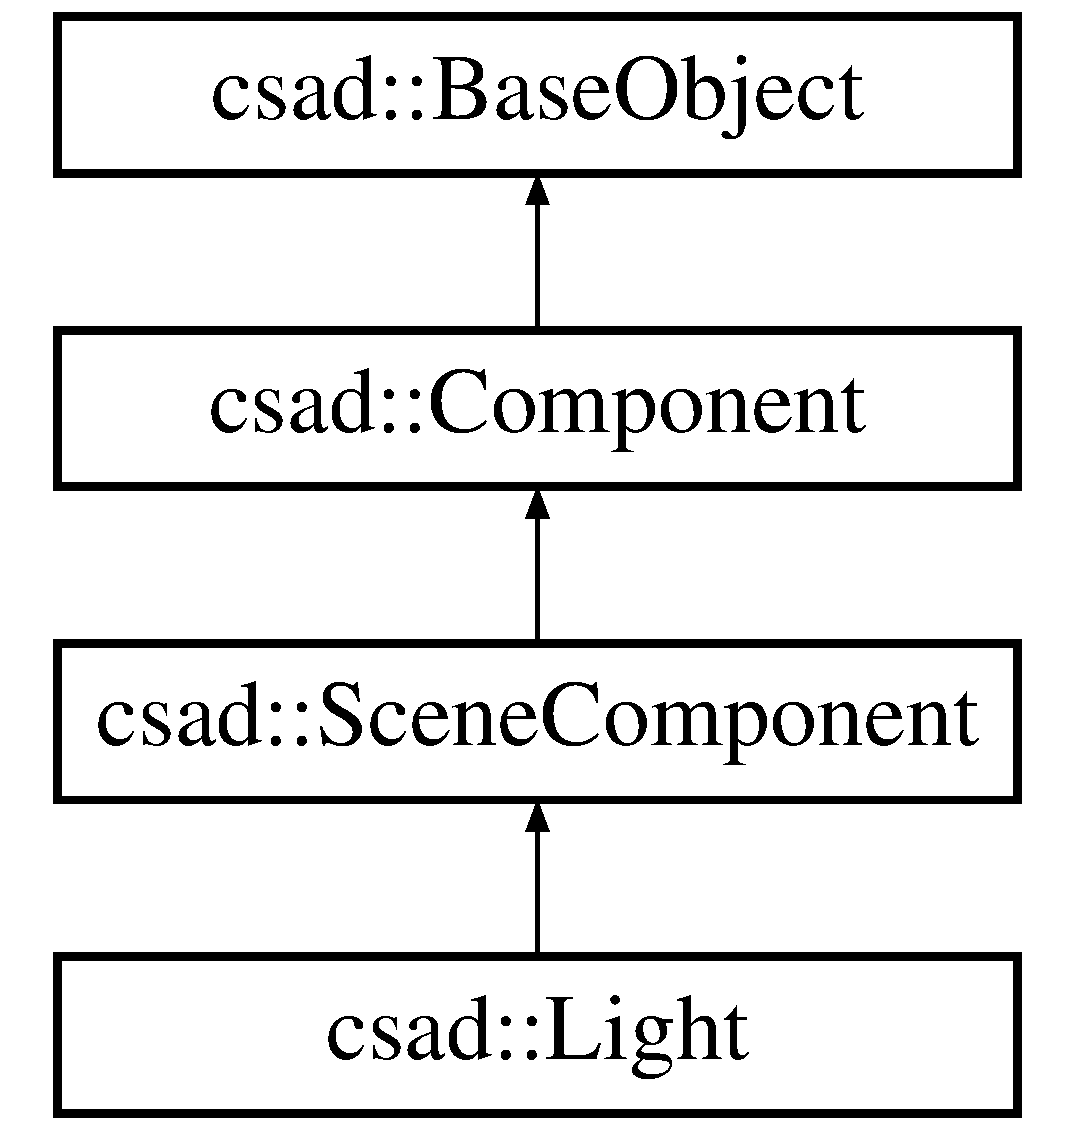
\includegraphics[height=4.000000cm]{classcsad_1_1_light}
\end{center}
\end{figure}
\subsection*{Public Types}
\begin{DoxyCompactItemize}
\item 
enum \hyperlink{classcsad_1_1_light_a00ff745cbb2a56fa7920b53acc068bf9}{Mode} \{ \hyperlink{classcsad_1_1_light_a00ff745cbb2a56fa7920b53acc068bf9a8869086b492b505de0a5ff65dfc79855}{Spot}, 
\hyperlink{classcsad_1_1_light_a00ff745cbb2a56fa7920b53acc068bf9a88b7d47bf52492997dd86c1b1db7e34d}{Point}, 
\hyperlink{classcsad_1_1_light_a00ff745cbb2a56fa7920b53acc068bf9a16c2d7e0e3d4f1609cb948b99d0ff72e}{Direct}
 \}
\begin{DoxyCompactList}\small\item\em \hyperlink{classcsad_1_1_light}{Light} mode. \end{DoxyCompactList}\end{DoxyCompactItemize}
\subsection*{Public Member Functions}
\begin{DoxyCompactItemize}
\item 
\hypertarget{classcsad_1_1_light_add5b8529c6d817ca14c9755ceaac6431}{\-\_\-\-F\-O\-R\-C\-E\-I\-N\-L\-I\-N\-E \hyperlink{classbt_1_1vector4f}{bt\-::vector4f} \& \hyperlink{classcsad_1_1_light_add5b8529c6d817ca14c9755ceaac6431}{ambient} ()}\label{classcsad_1_1_light_add5b8529c6d817ca14c9755ceaac6431}

\begin{DoxyCompactList}\small\item\em Ambient color. \end{DoxyCompactList}\item 
\hypertarget{classcsad_1_1_light_a9ec793f32b7e8a68f192c42e5289f7af}{\-\_\-\-F\-O\-R\-C\-E\-I\-N\-L\-I\-N\-E float \hyperlink{classcsad_1_1_light_a9ec793f32b7e8a68f192c42e5289f7af}{cutoff} ()}\label{classcsad_1_1_light_a9ec793f32b7e8a68f192c42e5289f7af}

\begin{DoxyCompactList}\small\item\em Return spot angle. \end{DoxyCompactList}\item 
\hypertarget{classcsad_1_1_light_a795de37f7b9287238560687ba3e37d62}{\-\_\-\-F\-O\-R\-C\-E\-I\-N\-L\-I\-N\-E \hyperlink{classbt_1_1vector4f}{bt\-::vector4f} \& \hyperlink{classcsad_1_1_light_a795de37f7b9287238560687ba3e37d62}{diffuse} ()}\label{classcsad_1_1_light_a795de37f7b9287238560687ba3e37d62}

\begin{DoxyCompactList}\small\item\em Diffuse color. \end{DoxyCompactList}\item 
\hypertarget{classcsad_1_1_light_ac0360f1db06e5f1027a0a42d8b9e7ac1}{\-\_\-\-F\-O\-R\-C\-E\-I\-N\-L\-I\-N\-E \hyperlink{classbt_1_1vector3f}{vector3f} \& \hyperlink{classcsad_1_1_light_ac0360f1db06e5f1027a0a42d8b9e7ac1}{direction} ()}\label{classcsad_1_1_light_ac0360f1db06e5f1027a0a42d8b9e7ac1}

\begin{DoxyCompactList}\small\item\em Return light direction. \end{DoxyCompactList}\item 
\hypertarget{classcsad_1_1_light_a4fc5e4e222d852a082cb32dddcab3c8b}{\-\_\-\-F\-O\-R\-C\-E\-I\-N\-L\-I\-N\-E unsigned int \hyperlink{classcsad_1_1_light_a4fc5e4e222d852a082cb32dddcab3c8b}{mode} ()}\label{classcsad_1_1_light_a4fc5e4e222d852a082cb32dddcab3c8b}

\begin{DoxyCompactList}\small\item\em Return light mode. \end{DoxyCompactList}\item 
\hypertarget{classcsad_1_1_light_a907bb4b27c9793e11ed5900bc6494680}{C\-S\-A\-D\-\_\-\-A\-P\-I void $\ast$ \hyperlink{classcsad_1_1_light_a907bb4b27c9793e11ed5900bc6494680}{set} (unsigned \-\_\-int32, void $\ast$)}\label{classcsad_1_1_light_a907bb4b27c9793e11ed5900bc6494680}

\begin{DoxyCompactList}\small\item\em used for any interface commands. \end{DoxyCompactList}\item 
\hypertarget{classcsad_1_1_light_a2122141dc16723e2cb41f304e07fd825}{C\-S\-A\-D\-\_\-\-A\-P\-I void \hyperlink{classcsad_1_1_light_a2122141dc16723e2cb41f304e07fd825}{set\-Cutoff} (float val)}\label{classcsad_1_1_light_a2122141dc16723e2cb41f304e07fd825}

\begin{DoxyCompactList}\small\item\em Set spot angle. \end{DoxyCompactList}\item 
\hypertarget{classcsad_1_1_light_a84be595e475849367973298993ba5a1b}{C\-S\-A\-D\-\_\-\-A\-P\-I void \hyperlink{classcsad_1_1_light_a84be595e475849367973298993ba5a1b}{set\-Direction} (\hyperlink{classbt_1_1vector3f}{vector3f} $\ast$dir)}\label{classcsad_1_1_light_a84be595e475849367973298993ba5a1b}

\begin{DoxyCompactList}\small\item\em Set light direction. \end{DoxyCompactList}\item 
\hypertarget{classcsad_1_1_light_ac499ecad2c29f85e08f5b0b14de9014c}{C\-S\-A\-D\-\_\-\-A\-P\-I void \hyperlink{classcsad_1_1_light_ac499ecad2c29f85e08f5b0b14de9014c}{set\-Mode} (unsigned int \hyperlink{classcsad_1_1_light_a4fc5e4e222d852a082cb32dddcab3c8b}{mode})}\label{classcsad_1_1_light_ac499ecad2c29f85e08f5b0b14de9014c}

\begin{DoxyCompactList}\small\item\em Define light mode. \end{DoxyCompactList}\item 
\hypertarget{classcsad_1_1_light_a6f2415fd8966df1ec467ba7595cec08e}{C\-S\-A\-D\-\_\-\-A\-P\-I void \hyperlink{classcsad_1_1_light_a6f2415fd8966df1ec467ba7595cec08e}{set\-Mode} (char $\ast$\hyperlink{classcsad_1_1_light_a4fc5e4e222d852a082cb32dddcab3c8b}{mode})}\label{classcsad_1_1_light_a6f2415fd8966df1ec467ba7595cec08e}

\begin{DoxyCompactList}\small\item\em Define light mode. \end{DoxyCompactList}\item 
\hypertarget{classcsad_1_1_light_a7df301de1fa1a05fa2e98751cdf6db2a}{\-\_\-\-F\-O\-R\-C\-E\-I\-N\-L\-I\-N\-E void \hyperlink{classcsad_1_1_light_a7df301de1fa1a05fa2e98751cdf6db2a}{set\-Mode} (const char $\ast$\hyperlink{classcsad_1_1_light_a4fc5e4e222d852a082cb32dddcab3c8b}{mode})}\label{classcsad_1_1_light_a7df301de1fa1a05fa2e98751cdf6db2a}

\begin{DoxyCompactList}\small\item\em Define light mode. \end{DoxyCompactList}\item 
\hypertarget{classcsad_1_1_light_a51da73272c28947c6367c8e1f0f7a4d3}{\-\_\-\-F\-O\-R\-C\-E\-I\-N\-L\-I\-N\-E \hyperlink{classbt_1_1vector4f}{bt\-::vector4f} \& \hyperlink{classcsad_1_1_light_a51da73272c28947c6367c8e1f0f7a4d3}{specular} ()}\label{classcsad_1_1_light_a51da73272c28947c6367c8e1f0f7a4d3}

\begin{DoxyCompactList}\small\item\em Specular color. \end{DoxyCompactList}\end{DoxyCompactItemize}
\subsection*{Additional Inherited Members}


\subsection{Detailed Description}
\hyperlink{classcsad_1_1_light}{Light} -\/ компонент определяющий источник света. 

For description in the configuration\-: \begin{DoxyVerb}  <Transform>
     <Light mode="режим" direction="направление"/>
  </Transform>
\end{DoxyVerb}


\begin{DoxySeeAlso}{See Also}
\hyperlink{classcsad_1_1_transform}{Transform}, \hyperlink{group__scene}{csad\-: scene} 
\end{DoxySeeAlso}


\subsection{Member Enumeration Documentation}
\hypertarget{classcsad_1_1_light_a00ff745cbb2a56fa7920b53acc068bf9}{\index{csad\-::\-Light@{csad\-::\-Light}!Mode@{Mode}}
\index{Mode@{Mode}!csad::Light@{csad\-::\-Light}}
\subsubsection[{Mode}]{\setlength{\rightskip}{0pt plus 5cm}enum {\bf csad\-::\-Light\-::\-Mode}}}\label{classcsad_1_1_light_a00ff745cbb2a56fa7920b53acc068bf9}


\hyperlink{classcsad_1_1_light}{Light} mode. 

\begin{Desc}
\item[Enumerator]\par
\begin{description}
\index{Spot@{Spot}!csad\-::\-Light@{csad\-::\-Light}}\index{csad\-::\-Light@{csad\-::\-Light}!Spot@{Spot}}\item[{\em 
\hypertarget{classcsad_1_1_light_a00ff745cbb2a56fa7920b53acc068bf9a8869086b492b505de0a5ff65dfc79855}{Spot}\label{classcsad_1_1_light_a00ff745cbb2a56fa7920b53acc068bf9a8869086b492b505de0a5ff65dfc79855}
}]Ranged light from point. \index{Point@{Point}!csad\-::\-Light@{csad\-::\-Light}}\index{csad\-::\-Light@{csad\-::\-Light}!Point@{Point}}\item[{\em 
\hypertarget{classcsad_1_1_light_a00ff745cbb2a56fa7920b53acc068bf9a88b7d47bf52492997dd86c1b1db7e34d}{Point}\label{classcsad_1_1_light_a00ff745cbb2a56fa7920b53acc068bf9a88b7d47bf52492997dd86c1b1db7e34d}
}]\hyperlink{classcsad_1_1_light}{Light} from point. \index{Direct@{Direct}!csad\-::\-Light@{csad\-::\-Light}}\index{csad\-::\-Light@{csad\-::\-Light}!Direct@{Direct}}\item[{\em 
\hypertarget{classcsad_1_1_light_a00ff745cbb2a56fa7920b53acc068bf9a16c2d7e0e3d4f1609cb948b99d0ff72e}{Direct}\label{classcsad_1_1_light_a00ff745cbb2a56fa7920b53acc068bf9a16c2d7e0e3d4f1609cb948b99d0ff72e}
}]Linear light. \end{description}
\end{Desc}

\hypertarget{classcsad_1_1_lighting_model}{\section{csad\-:\-:Lighting\-Model Class Reference}
\label{classcsad_1_1_lighting_model}\index{csad\-::\-Lighting\-Model@{csad\-::\-Lighting\-Model}}
}


\hyperlink{classcsad_1_1_lighting_model}{Lighting\-Model} -\/ группа освещения.  


Inheritance diagram for csad\-:\-:Lighting\-Model\-:\begin{figure}[H]
\begin{center}
\leavevmode
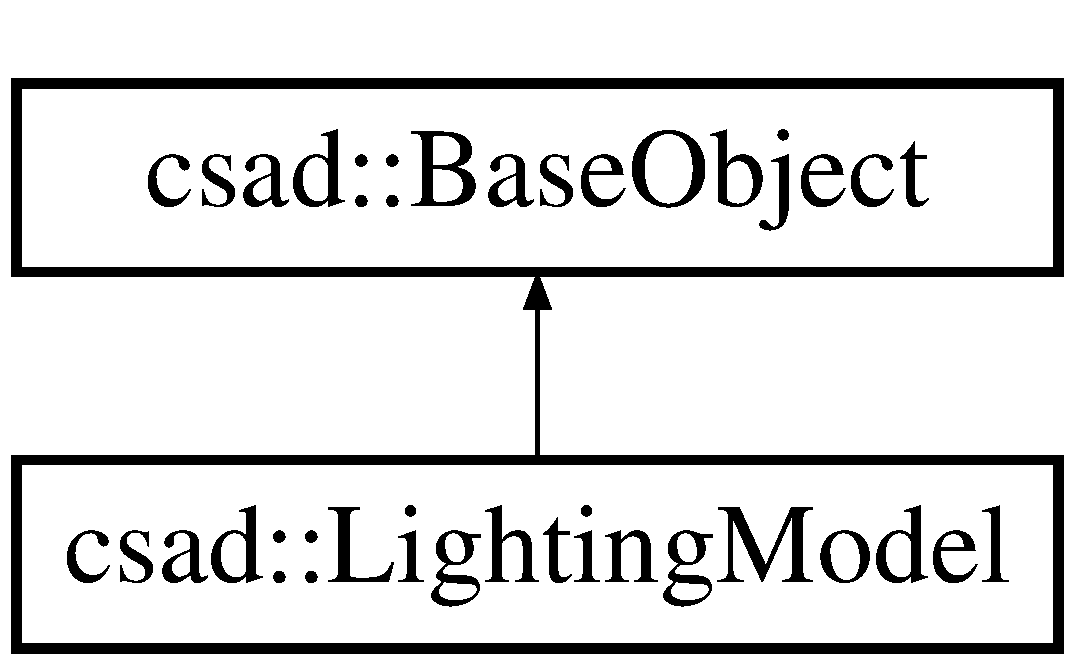
\includegraphics[height=2.000000cm]{classcsad_1_1_lighting_model}
\end{center}
\end{figure}
\subsection*{Public Member Functions}
\begin{DoxyCompactItemize}
\item 
\hypertarget{classcsad_1_1_lighting_model_ab597f6f4d2e18b8ff581c0dfe6d02639}{\hyperlink{classbt_1_1_void_vector}{List\-Lightings} \& \hyperlink{classcsad_1_1_lighting_model_ab597f6f4d2e18b8ff581c0dfe6d02639}{lights} ()}\label{classcsad_1_1_lighting_model_ab597f6f4d2e18b8ff581c0dfe6d02639}

\begin{DoxyCompactList}\small\item\em lights in lighting model \end{DoxyCompactList}\item 
\hypertarget{classcsad_1_1_lighting_model_abbb9dd1011eba62aff6f9afc5ae1415e}{C\-S\-A\-D\-\_\-\-A\-P\-I void $\ast$ \hyperlink{classcsad_1_1_lighting_model_abbb9dd1011eba62aff6f9afc5ae1415e}{set} (unsigned \-\_\-int32, void $\ast$)}\label{classcsad_1_1_lighting_model_abbb9dd1011eba62aff6f9afc5ae1415e}

\begin{DoxyCompactList}\small\item\em used for any interface commands. \end{DoxyCompactList}\item 
\hypertarget{classcsad_1_1_lighting_model_a9b28bbef8850d6361593d37b63ec8668}{C\-S\-A\-D\-\_\-\-A\-P\-I \hyperlink{classcsad_1_1_lighting_model}{Lighting\-Model} \& \hyperlink{classcsad_1_1_lighting_model_a9b28bbef8850d6361593d37b63ec8668}{set\-Light} (unsigned int id, char $\ast$name)}\label{classcsad_1_1_lighting_model_a9b28bbef8850d6361593d37b63ec8668}

\begin{DoxyCompactList}\small\item\em use light in lighting model \end{DoxyCompactList}\item 
\hypertarget{classcsad_1_1_lighting_model_a226c35135524c3882081629f8f0696b6}{\-\_\-\-F\-O\-R\-C\-E\-I\-N\-L\-I\-N\-E \hyperlink{classcsad_1_1_lighting_model}{Lighting\-Model} \& \hyperlink{classcsad_1_1_lighting_model_a226c35135524c3882081629f8f0696b6}{set\-Light} (unsigned int id, const char $\ast$name)}\label{classcsad_1_1_lighting_model_a226c35135524c3882081629f8f0696b6}

\begin{DoxyCompactList}\small\item\em use light in lighting model \end{DoxyCompactList}\item 
\hypertarget{classcsad_1_1_lighting_model_ac3687ba56ddf122657bf3a148e74d934}{C\-S\-A\-D\-\_\-\-A\-P\-I \hyperlink{classcsad_1_1_lighting_model}{Lighting\-Model} \& \hyperlink{classcsad_1_1_lighting_model_ac3687ba56ddf122657bf3a148e74d934}{set\-Light} (unsigned int id, \hyperlink{classcsad_1_1_light}{Light} $\ast$light)}\label{classcsad_1_1_lighting_model_ac3687ba56ddf122657bf3a148e74d934}

\begin{DoxyCompactList}\small\item\em use light in lighting model \end{DoxyCompactList}\end{DoxyCompactItemize}
\subsection*{Additional Inherited Members}


\subsection{Detailed Description}
\hyperlink{classcsad_1_1_lighting_model}{Lighting\-Model} -\/ группа освещения. 

For description in the configuration\-: \begin{DoxyVerb}  <Scene>
     <Transform name="name of light">
        <Light />
     </Transform>
     <LightingModel name="name mode" light0="name of light"/>
  </Scene>
\end{DoxyVerb}


\begin{DoxySeeAlso}{See Also}
\hyperlink{classcsad_1_1_scene}{Scene}, \hyperlink{group__scene}{csad\-: scene} 
\end{DoxySeeAlso}

\hypertarget{classcsad_1_1_material}{\section{csad\-:\-:Material Class Reference}
\label{classcsad_1_1_material}\index{csad\-::\-Material@{csad\-::\-Material}}
}


\hyperlink{classcsad_1_1_material}{Material} -\/ the object of material.  


Inheritance diagram for csad\-:\-:Material\-:\begin{figure}[H]
\begin{center}
\leavevmode
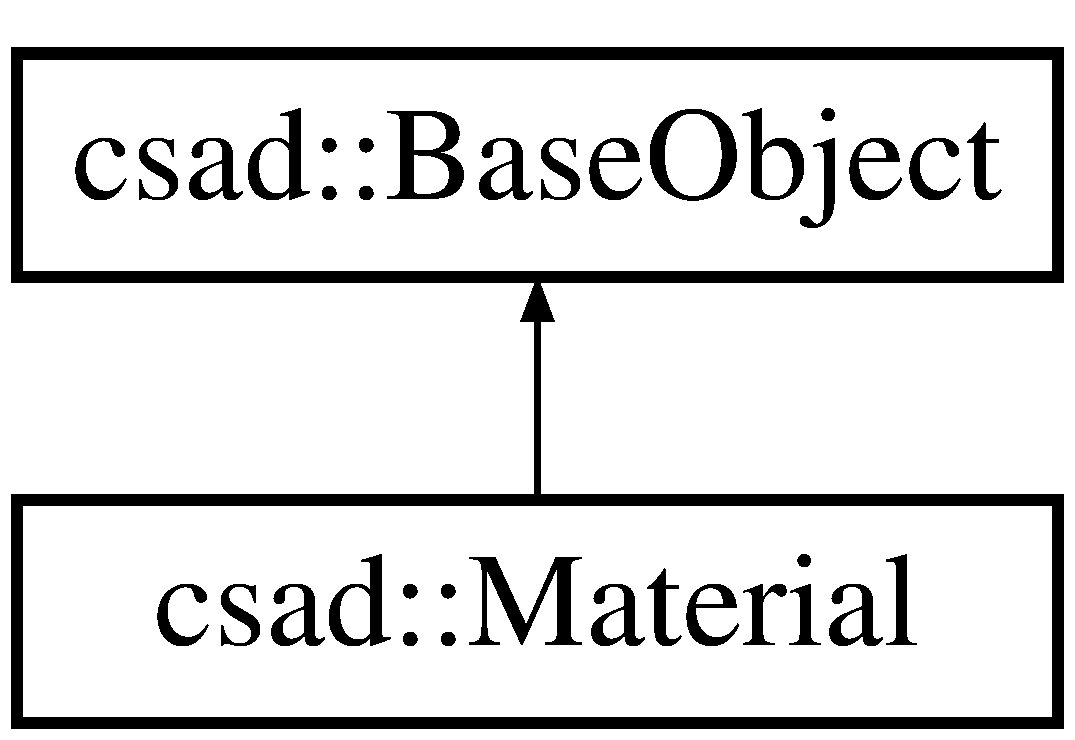
\includegraphics[height=2.000000cm]{classcsad_1_1_material}
\end{center}
\end{figure}
\subsection*{Public Types}
\begin{DoxyCompactItemize}
\item 
enum \hyperlink{classcsad_1_1_material_a2bce1dfef3df915e073ae55bfff7d8a0}{Blend} \{ \\*
\hyperlink{classcsad_1_1_material_a2bce1dfef3df915e073ae55bfff7d8a0a966f095b1846315c6f6cde12b031f1fb}{N\-O\-N\-E} =-\/1, 
\hyperlink{classcsad_1_1_material_a2bce1dfef3df915e073ae55bfff7d8a0a22db8c064c2fd8d175f88e5b86ede25a}{Z\-E\-R\-O} =0, 
\hyperlink{classcsad_1_1_material_a2bce1dfef3df915e073ae55bfff7d8a0a14674ed9ce3582a9570cf2b33fc32bbd}{O\-N\-E} =1, 
\hyperlink{classcsad_1_1_material_a2bce1dfef3df915e073ae55bfff7d8a0a6401f148d0822e5e15e864fb14b58253}{N\-E\-V\-E\-R} =0x0200, 
\\*
\hyperlink{classcsad_1_1_material_a2bce1dfef3df915e073ae55bfff7d8a0a7d5b187c7f4ffab97f236f417479ed27}{L\-E\-S\-S} =0x0201, 
\hyperlink{classcsad_1_1_material_a2bce1dfef3df915e073ae55bfff7d8a0ab345773c791355de704fac9723195fff}{E\-Q\-U\-A\-L} =0x0202
, \hyperlink{classcsad_1_1_material_a2bce1dfef3df915e073ae55bfff7d8a0a6e3351430b1e83cd6b2af6d8821cfb0f}{G\-R\-E\-A\-T\-E\-R} =0x0204
, \hyperlink{classcsad_1_1_material_a2bce1dfef3df915e073ae55bfff7d8a0af9eeec030f40c4ee83fef8310e0f6d28}{A\-L\-W\-A\-Y\-S} =0x0207, 
\\*
\hyperlink{classcsad_1_1_material_a2bce1dfef3df915e073ae55bfff7d8a0aa85c52eafaf66d1439736b3b450381d7}{S\-R\-C\-\_\-\-C\-O\-L\-O\-R} =0x0300, 
\hyperlink{classcsad_1_1_material_a2bce1dfef3df915e073ae55bfff7d8a0a9ad72af9631faf04057b303f4aecfb51}{O\-N\-E\-\_\-\-M\-I\-N\-U\-S\-\_\-\-S\-R\-C\-\_\-\-C\-O\-L\-O\-R} =0x0301, 
\hyperlink{classcsad_1_1_material_a2bce1dfef3df915e073ae55bfff7d8a0a11cfdcf0642314ebfeab5e1e0ed4c3b2}{S\-R\-C\-\_\-\-A\-L\-P\-H\-A} =0x0302, 
\hyperlink{classcsad_1_1_material_a2bce1dfef3df915e073ae55bfff7d8a0a1239172d8147d0a51fae5dc0f7cd9b70}{O\-N\-E\-\_\-\-M\-I\-N\-U\-S\-\_\-\-S\-R\-C\-\_\-\-A\-L\-P\-H\-A} =0x0303, 
\\*
\hyperlink{classcsad_1_1_material_a2bce1dfef3df915e073ae55bfff7d8a0a672cbfec237b6e2ded732e59750f4250}{D\-S\-T\-\_\-\-A\-L\-P\-H\-A} =0x0304, 
\hyperlink{classcsad_1_1_material_a2bce1dfef3df915e073ae55bfff7d8a0ab5fb7c0624277d05f211a1ada5ae8d91}{O\-N\-E\-\_\-\-M\-I\-N\-U\-S\-\_\-\-D\-S\-T\-\_\-\-A\-L\-P\-H\-A} =0x0305, 
\hyperlink{classcsad_1_1_material_a2bce1dfef3df915e073ae55bfff7d8a0acffd3ee341f415609d1a9cc0bfacbd1a}{D\-S\-T\-\_\-\-C\-O\-L\-O\-R} =0x0306, 
\hyperlink{classcsad_1_1_material_a2bce1dfef3df915e073ae55bfff7d8a0ae35a4e345bfeefa08ea54097aefdc438}{O\-N\-E\-\_\-\-M\-I\-N\-U\-S\-\_\-\-D\-S\-T\-\_\-\-C\-O\-L\-O\-R} =0x0307
 \}
\begin{DoxyCompactList}\small\item\em Blend functions. \end{DoxyCompactList}\end{DoxyCompactItemize}
\subsection*{Public Member Functions}
\begin{DoxyCompactItemize}
\item 
\hypertarget{classcsad_1_1_material_a267a8e919aa3f869b4d4277707a57f94}{\-\_\-\-F\-O\-R\-C\-E\-I\-N\-L\-I\-N\-E \hyperlink{classbt_1_1vector4f}{vector4f} \hyperlink{classcsad_1_1_material_a267a8e919aa3f869b4d4277707a57f94}{get\-Diffuse} ()}\label{classcsad_1_1_material_a267a8e919aa3f869b4d4277707a57f94}

\begin{DoxyCompactList}\small\item\em return diffuse color. \end{DoxyCompactList}\item 
\hypertarget{classcsad_1_1_material_a0cb5cb5f3ace5c2faf5db9ffdffb3f0c}{C\-S\-A\-D\-\_\-\-A\-P\-I const char $\ast$ \hyperlink{classcsad_1_1_material_a0cb5cb5f3ace5c2faf5db9ffdffb3f0c}{get\-Name} ()}\label{classcsad_1_1_material_a0cb5cb5f3ace5c2faf5db9ffdffb3f0c}

\begin{DoxyCompactList}\small\item\em return material name \end{DoxyCompactList}\item 
\hypertarget{classcsad_1_1_material_a192f44e50f85ed9c80b5e507188b4ab9}{C\-S\-A\-D\-\_\-\-A\-P\-I \hyperlink{classcsad_1_1_texture2_d}{Texture2\-D} $\ast$ \hyperlink{classcsad_1_1_material_a192f44e50f85ed9c80b5e507188b4ab9}{get\-Texture2\-D} (unsigned int id=0)}\label{classcsad_1_1_material_a192f44e50f85ed9c80b5e507188b4ab9}

\begin{DoxyCompactList}\small\item\em return texture. \end{DoxyCompactList}\item 
\hypertarget{classcsad_1_1_material_a09fd6a6298ddd9eeb930eb270c3ea58f}{C\-S\-A\-D\-\_\-\-A\-P\-I \hyperlink{classbt_1_1matrix4f}{bt\-::matrix4f} $\ast$ \hyperlink{classcsad_1_1_material_a09fd6a6298ddd9eeb930eb270c3ea58f}{get\-Texture\-Matrix} (unsigned int id=0)}\label{classcsad_1_1_material_a09fd6a6298ddd9eeb930eb270c3ea58f}

\begin{DoxyCompactList}\small\item\em returns the matrix texture coordinates \end{DoxyCompactList}\item 
\hypertarget{classcsad_1_1_material_a7b73ef9d1d2b1fb28249a8067d4976db}{\-\_\-\-F\-O\-R\-C\-E\-I\-N\-L\-I\-N\-E bool \hyperlink{classcsad_1_1_material_a7b73ef9d1d2b1fb28249a8067d4976db}{is\-Light} ()}\label{classcsad_1_1_material_a7b73ef9d1d2b1fb28249a8067d4976db}

\begin{DoxyCompactList}\small\item\em Is emit light. \end{DoxyCompactList}\item 
\hypertarget{classcsad_1_1_material_a82d954d2ec389cd90f52d3a1bdbb3b87}{C\-S\-A\-D\-\_\-\-A\-P\-I void $\ast$ \hyperlink{classcsad_1_1_material_a82d954d2ec389cd90f52d3a1bdbb3b87}{set} (unsigned \-\_\-int32, void $\ast$)}\label{classcsad_1_1_material_a82d954d2ec389cd90f52d3a1bdbb3b87}

\begin{DoxyCompactList}\small\item\em used for any interface commands. \end{DoxyCompactList}\item 
\hypertarget{classcsad_1_1_material_a85b4dfb6502863b0b896352b29d0bc74}{C\-S\-A\-D\-\_\-\-A\-P\-I void \hyperlink{classcsad_1_1_material_a85b4dfb6502863b0b896352b29d0bc74}{set\-Alpha} (int func, float ref=0.\-5f)}\label{classcsad_1_1_material_a85b4dfb6502863b0b896352b29d0bc74}

\begin{DoxyCompactList}\small\item\em set alpha function parameters \end{DoxyCompactList}\item 
\hypertarget{classcsad_1_1_material_a71d48f2425e2fc61ef2546350a70e88e}{C\-S\-A\-D\-\_\-\-A\-P\-I void \hyperlink{classcsad_1_1_material_a71d48f2425e2fc61ef2546350a70e88e}{set\-Alpha} (char $\ast$func=0, float ref=0.\-5f)}\label{classcsad_1_1_material_a71d48f2425e2fc61ef2546350a70e88e}

\begin{DoxyCompactList}\small\item\em set alpha function parameters by name \end{DoxyCompactList}\item 
\hypertarget{classcsad_1_1_material_a7b0a7a87159a7dd02dfd809404ed53cc}{C\-S\-A\-D\-\_\-\-A\-P\-I void \hyperlink{classcsad_1_1_material_a7b0a7a87159a7dd02dfd809404ed53cc}{set\-Ambient} (\hyperlink{classbt_1_1vector4f}{vector4f} \&color)}\label{classcsad_1_1_material_a7b0a7a87159a7dd02dfd809404ed53cc}

\begin{DoxyCompactList}\small\item\em set ambient color \end{DoxyCompactList}\item 
\hypertarget{classcsad_1_1_material_a1d6d882d09da03fa06ed88c0a370e330}{\-\_\-\-F\-O\-R\-C\-E\-I\-N\-L\-I\-N\-E void \hyperlink{classcsad_1_1_material_a1d6d882d09da03fa06ed88c0a370e330}{set\-Ambient} (float r, float g, float b, float a)}\label{classcsad_1_1_material_a1d6d882d09da03fa06ed88c0a370e330}

\begin{DoxyCompactList}\small\item\em set ambient color \end{DoxyCompactList}\item 
\hypertarget{classcsad_1_1_material_a11344c6e5f8d9c76c2cad2097e3bb64a}{C\-S\-A\-D\-\_\-\-A\-P\-I void \hyperlink{classcsad_1_1_material_a11344c6e5f8d9c76c2cad2097e3bb64a}{set\-Blend} (int src=0, int dst=0)}\label{classcsad_1_1_material_a11344c6e5f8d9c76c2cad2097e3bb64a}

\begin{DoxyCompactList}\small\item\em set blend function parameters \end{DoxyCompactList}\item 
\hypertarget{classcsad_1_1_material_aeb022f5dfdf05f54b1ba928844d40d2f}{C\-S\-A\-D\-\_\-\-A\-P\-I void \hyperlink{classcsad_1_1_material_aeb022f5dfdf05f54b1ba928844d40d2f}{set\-Blend} (char $\ast$src=0, char $\ast$dst=0)}\label{classcsad_1_1_material_aeb022f5dfdf05f54b1ba928844d40d2f}

\begin{DoxyCompactList}\small\item\em set blend function parameters by name \end{DoxyCompactList}\item 
\hypertarget{classcsad_1_1_material_ac0016039da7c346bfbae8c6e6bf41932}{C\-S\-A\-D\-\_\-\-A\-P\-I void \hyperlink{classcsad_1_1_material_ac0016039da7c346bfbae8c6e6bf41932}{set\-Depth} (int func)}\label{classcsad_1_1_material_ac0016039da7c346bfbae8c6e6bf41932}

\begin{DoxyCompactList}\small\item\em Depth test function. \end{DoxyCompactList}\item 
\hypertarget{classcsad_1_1_material_a70f19ccf1cd351c42e4c500bcbc4efe1}{C\-S\-A\-D\-\_\-\-A\-P\-I void \hyperlink{classcsad_1_1_material_a70f19ccf1cd351c42e4c500bcbc4efe1}{set\-Depth\-Write} (bool \hyperlink{classcsad_1_1_base_object_a588a28a35b2aefa0a833405f152d73e4}{write})}\label{classcsad_1_1_material_a70f19ccf1cd351c42e4c500bcbc4efe1}

\begin{DoxyCompactList}\small\item\em Enable or disable depth write. \end{DoxyCompactList}\item 
\hypertarget{classcsad_1_1_material_ab5d322bd830b4adf42acdf663accc544}{C\-S\-A\-D\-\_\-\-A\-P\-I void \hyperlink{classcsad_1_1_material_ab5d322bd830b4adf42acdf663accc544}{set\-Diffuse} (\hyperlink{classbt_1_1vector4f}{vector4f} \&color)}\label{classcsad_1_1_material_ab5d322bd830b4adf42acdf663accc544}

\begin{DoxyCompactList}\small\item\em set color. \end{DoxyCompactList}\item 
\hypertarget{classcsad_1_1_material_a49ce166a7ab43f03e0de583308f1f956}{\-\_\-\-F\-O\-R\-C\-E\-I\-N\-L\-I\-N\-E void \hyperlink{classcsad_1_1_material_a49ce166a7ab43f03e0de583308f1f956}{set\-Diffuse} (float r, float g, float b, float a)}\label{classcsad_1_1_material_a49ce166a7ab43f03e0de583308f1f956}

\begin{DoxyCompactList}\small\item\em set color. \end{DoxyCompactList}\item 
\hypertarget{classcsad_1_1_material_af7522a5ab3b5fb514940e1ea0889a27c}{C\-S\-A\-D\-\_\-\-A\-P\-I void \hyperlink{classcsad_1_1_material_af7522a5ab3b5fb514940e1ea0889a27c}{set\-Emission} (\hyperlink{classbt_1_1vector4f}{vector4f} \&color)}\label{classcsad_1_1_material_af7522a5ab3b5fb514940e1ea0889a27c}

\begin{DoxyCompactList}\small\item\em set emission color \end{DoxyCompactList}\item 
\hypertarget{classcsad_1_1_material_a2917427c5332354bb23fc9c3d535f075}{\-\_\-\-F\-O\-R\-C\-E\-I\-N\-L\-I\-N\-E void \hyperlink{classcsad_1_1_material_a2917427c5332354bb23fc9c3d535f075}{set\-Emission} (float r, float g, float b, float a)}\label{classcsad_1_1_material_a2917427c5332354bb23fc9c3d535f075}

\begin{DoxyCompactList}\small\item\em set emission color \end{DoxyCompactList}\item 
\hypertarget{classcsad_1_1_material_ac9450c272697b766603235851dd33f03}{C\-S\-A\-D\-\_\-\-A\-P\-I void \hyperlink{classcsad_1_1_material_ac9450c272697b766603235851dd33f03}{set\-Light} (bool val)}\label{classcsad_1_1_material_ac9450c272697b766603235851dd33f03}

\begin{DoxyCompactList}\small\item\em Emit light. \end{DoxyCompactList}\item 
\hypertarget{classcsad_1_1_material_ab077e1d2feb25d8204d56343e1c45738}{C\-S\-A\-D\-\_\-\-A\-P\-I void \hyperlink{classcsad_1_1_material_ab077e1d2feb25d8204d56343e1c45738}{set\-Line\-With} (float val)}\label{classcsad_1_1_material_ab077e1d2feb25d8204d56343e1c45738}

\begin{DoxyCompactList}\small\item\em set line with parameter \end{DoxyCompactList}\item 
\hypertarget{classcsad_1_1_material_a5c270b64f924b16f4c7fd3769c281aea}{C\-S\-A\-D\-\_\-\-A\-P\-I void \hyperlink{classcsad_1_1_material_a5c270b64f924b16f4c7fd3769c281aea}{set\-Point\-Size} (float val)}\label{classcsad_1_1_material_a5c270b64f924b16f4c7fd3769c281aea}

\begin{DoxyCompactList}\small\item\em set point size parameter \end{DoxyCompactList}\item 
\hypertarget{classcsad_1_1_material_a8ed3e9ebe5332050223218fa01855f4d}{C\-S\-A\-D\-\_\-\-A\-P\-I void \hyperlink{classcsad_1_1_material_a8ed3e9ebe5332050223218fa01855f4d}{set\-Specular} (\hyperlink{classbt_1_1vector4f}{vector4f} \&color)}\label{classcsad_1_1_material_a8ed3e9ebe5332050223218fa01855f4d}

\begin{DoxyCompactList}\small\item\em set specular color \end{DoxyCompactList}\item 
\hypertarget{classcsad_1_1_material_a64c90cd4ca7d5bb8c6966d3eba7dcf06}{\-\_\-\-F\-O\-R\-C\-E\-I\-N\-L\-I\-N\-E void \hyperlink{classcsad_1_1_material_a64c90cd4ca7d5bb8c6966d3eba7dcf06}{set\-Specular} (float r, float g, float b, float a)}\label{classcsad_1_1_material_a64c90cd4ca7d5bb8c6966d3eba7dcf06}

\begin{DoxyCompactList}\small\item\em set specular color \end{DoxyCompactList}\item 
\hypertarget{classcsad_1_1_material_a70d15f44aaa33b668b6e832aab38984b}{C\-S\-A\-D\-\_\-\-A\-P\-I int \hyperlink{classcsad_1_1_material_a70d15f44aaa33b668b6e832aab38984b}{set\-Texture2\-D} (\hyperlink{classcsad_1_1_texture2_d}{Texture2\-D} $\ast$texture, unsigned int id=0)}\label{classcsad_1_1_material_a70d15f44aaa33b668b6e832aab38984b}

\begin{DoxyCompactList}\small\item\em setting the texture, the id number of the layer for multitexturing. \end{DoxyCompactList}\item 
\hypertarget{classcsad_1_1_material_afaf6612ca664c0073a7e6d6d15a1185e}{C\-S\-A\-D\-\_\-\-A\-P\-I int \hyperlink{classcsad_1_1_material_afaf6612ca664c0073a7e6d6d15a1185e}{set\-Texture2\-D} (char $\ast$name, unsigned int id=0)}\label{classcsad_1_1_material_afaf6612ca664c0073a7e6d6d15a1185e}

\begin{DoxyCompactList}\small\item\em setting the texture, the id number of the layer for multitexturing. \end{DoxyCompactList}\item 
\hypertarget{classcsad_1_1_material_a814aec72ba2c958915ebcd9864cd39b5}{C\-S\-A\-D\-\_\-\-A\-P\-I void \hyperlink{classcsad_1_1_material_a814aec72ba2c958915ebcd9864cd39b5}{set\-Texture\-Matrix} (\hyperlink{classbt_1_1matrix4f}{bt\-::matrix4f} \&matrix, unsigned int id=0)}\label{classcsad_1_1_material_a814aec72ba2c958915ebcd9864cd39b5}

\begin{DoxyCompactList}\small\item\em sets the matrix to transform texture coordinates \end{DoxyCompactList}\item 
\hypertarget{classcsad_1_1_material_ab2f143ec735060d18c128f6617889d5e}{C\-S\-A\-D\-\_\-\-A\-P\-I void \hyperlink{classcsad_1_1_material_ab2f143ec735060d18c128f6617889d5e}{set\-Texture\-Rect} (\hyperlink{classbt_1_1vector4f}{bt\-::vector4f} \&rect, unsigned int id=0)}\label{classcsad_1_1_material_ab2f143ec735060d18c128f6617889d5e}

\begin{DoxyCompactList}\small\item\em sets the matrix to transform texture coordinates as the area of the texture \end{DoxyCompactList}\end{DoxyCompactItemize}


\subsection{Detailed Description}
\hyperlink{classcsad_1_1_material}{Material} -\/ the object of material. 

\begin{DoxyVerb}  <Material name="material name" color="0.1 1.0 1.0 1.0" ambient="0.0 0.0 0.0 1.0" src="SRC_ALPHA" dst="DST_COLOR" />
\end{DoxyVerb}
 \begin{DoxySeeAlso}{See Also}
\hyperlink{group__scene}{csad\-: scene} 
\end{DoxySeeAlso}


\subsection{Member Enumeration Documentation}
\hypertarget{classcsad_1_1_material_a2bce1dfef3df915e073ae55bfff7d8a0}{\index{csad\-::\-Material@{csad\-::\-Material}!Blend@{Blend}}
\index{Blend@{Blend}!csad::Material@{csad\-::\-Material}}
\subsubsection[{Blend}]{\setlength{\rightskip}{0pt plus 5cm}enum {\bf csad\-::\-Material\-::\-Blend}}}\label{classcsad_1_1_material_a2bce1dfef3df915e073ae55bfff7d8a0}


Blend functions. 

\begin{Desc}
\item[Enumerator]\par
\begin{description}
\index{N\-O\-N\-E@{N\-O\-N\-E}!csad\-::\-Material@{csad\-::\-Material}}\index{csad\-::\-Material@{csad\-::\-Material}!N\-O\-N\-E@{N\-O\-N\-E}}\item[{\em 
\hypertarget{classcsad_1_1_material_a2bce1dfef3df915e073ae55bfff7d8a0a966f095b1846315c6f6cde12b031f1fb}{N\-O\-N\-E}\label{classcsad_1_1_material_a2bce1dfef3df915e073ae55bfff7d8a0a966f095b1846315c6f6cde12b031f1fb}
}]Not use. \index{Z\-E\-R\-O@{Z\-E\-R\-O}!csad\-::\-Material@{csad\-::\-Material}}\index{csad\-::\-Material@{csad\-::\-Material}!Z\-E\-R\-O@{Z\-E\-R\-O}}\item[{\em 
\hypertarget{classcsad_1_1_material_a2bce1dfef3df915e073ae55bfff7d8a0a22db8c064c2fd8d175f88e5b86ede25a}{Z\-E\-R\-O}\label{classcsad_1_1_material_a2bce1dfef3df915e073ae55bfff7d8a0a22db8c064c2fd8d175f88e5b86ede25a}
}]Use parameter zero. \index{O\-N\-E@{O\-N\-E}!csad\-::\-Material@{csad\-::\-Material}}\index{csad\-::\-Material@{csad\-::\-Material}!O\-N\-E@{O\-N\-E}}\item[{\em 
\hypertarget{classcsad_1_1_material_a2bce1dfef3df915e073ae55bfff7d8a0a14674ed9ce3582a9570cf2b33fc32bbd}{O\-N\-E}\label{classcsad_1_1_material_a2bce1dfef3df915e073ae55bfff7d8a0a14674ed9ce3582a9570cf2b33fc32bbd}
}]Use parameter one. \index{N\-E\-V\-E\-R@{N\-E\-V\-E\-R}!csad\-::\-Material@{csad\-::\-Material}}\index{csad\-::\-Material@{csad\-::\-Material}!N\-E\-V\-E\-R@{N\-E\-V\-E\-R}}\item[{\em 
\hypertarget{classcsad_1_1_material_a2bce1dfef3df915e073ae55bfff7d8a0a6401f148d0822e5e15e864fb14b58253}{N\-E\-V\-E\-R}\label{classcsad_1_1_material_a2bce1dfef3df915e073ae55bfff7d8a0a6401f148d0822e5e15e864fb14b58253}
}]If never. \index{L\-E\-S\-S@{L\-E\-S\-S}!csad\-::\-Material@{csad\-::\-Material}}\index{csad\-::\-Material@{csad\-::\-Material}!L\-E\-S\-S@{L\-E\-S\-S}}\item[{\em 
\hypertarget{classcsad_1_1_material_a2bce1dfef3df915e073ae55bfff7d8a0a7d5b187c7f4ffab97f236f417479ed27}{L\-E\-S\-S}\label{classcsad_1_1_material_a2bce1dfef3df915e073ae55bfff7d8a0a7d5b187c7f4ffab97f236f417479ed27}
}]If less. \index{E\-Q\-U\-A\-L@{E\-Q\-U\-A\-L}!csad\-::\-Material@{csad\-::\-Material}}\index{csad\-::\-Material@{csad\-::\-Material}!E\-Q\-U\-A\-L@{E\-Q\-U\-A\-L}}\item[{\em 
\hypertarget{classcsad_1_1_material_a2bce1dfef3df915e073ae55bfff7d8a0ab345773c791355de704fac9723195fff}{E\-Q\-U\-A\-L}\label{classcsad_1_1_material_a2bce1dfef3df915e073ae55bfff7d8a0ab345773c791355de704fac9723195fff}
}]If equal. \index{G\-R\-E\-A\-T\-E\-R@{G\-R\-E\-A\-T\-E\-R}!csad\-::\-Material@{csad\-::\-Material}}\index{csad\-::\-Material@{csad\-::\-Material}!G\-R\-E\-A\-T\-E\-R@{G\-R\-E\-A\-T\-E\-R}}\item[{\em 
\hypertarget{classcsad_1_1_material_a2bce1dfef3df915e073ae55bfff7d8a0a6e3351430b1e83cd6b2af6d8821cfb0f}{G\-R\-E\-A\-T\-E\-R}\label{classcsad_1_1_material_a2bce1dfef3df915e073ae55bfff7d8a0a6e3351430b1e83cd6b2af6d8821cfb0f}
}]If greater. \index{A\-L\-W\-A\-Y\-S@{A\-L\-W\-A\-Y\-S}!csad\-::\-Material@{csad\-::\-Material}}\index{csad\-::\-Material@{csad\-::\-Material}!A\-L\-W\-A\-Y\-S@{A\-L\-W\-A\-Y\-S}}\item[{\em 
\hypertarget{classcsad_1_1_material_a2bce1dfef3df915e073ae55bfff7d8a0af9eeec030f40c4ee83fef8310e0f6d28}{A\-L\-W\-A\-Y\-S}\label{classcsad_1_1_material_a2bce1dfef3df915e073ae55bfff7d8a0af9eeec030f40c4ee83fef8310e0f6d28}
}]always \index{S\-R\-C\-\_\-\-C\-O\-L\-O\-R@{S\-R\-C\-\_\-\-C\-O\-L\-O\-R}!csad\-::\-Material@{csad\-::\-Material}}\index{csad\-::\-Material@{csad\-::\-Material}!S\-R\-C\-\_\-\-C\-O\-L\-O\-R@{S\-R\-C\-\_\-\-C\-O\-L\-O\-R}}\item[{\em 
\hypertarget{classcsad_1_1_material_a2bce1dfef3df915e073ae55bfff7d8a0aa85c52eafaf66d1439736b3b450381d7}{S\-R\-C\-\_\-\-C\-O\-L\-O\-R}\label{classcsad_1_1_material_a2bce1dfef3df915e073ae55bfff7d8a0aa85c52eafaf66d1439736b3b450381d7}
}]Use parameter from source. \index{O\-N\-E\-\_\-\-M\-I\-N\-U\-S\-\_\-\-S\-R\-C\-\_\-\-C\-O\-L\-O\-R@{O\-N\-E\-\_\-\-M\-I\-N\-U\-S\-\_\-\-S\-R\-C\-\_\-\-C\-O\-L\-O\-R}!csad\-::\-Material@{csad\-::\-Material}}\index{csad\-::\-Material@{csad\-::\-Material}!O\-N\-E\-\_\-\-M\-I\-N\-U\-S\-\_\-\-S\-R\-C\-\_\-\-C\-O\-L\-O\-R@{O\-N\-E\-\_\-\-M\-I\-N\-U\-S\-\_\-\-S\-R\-C\-\_\-\-C\-O\-L\-O\-R}}\item[{\em 
\hypertarget{classcsad_1_1_material_a2bce1dfef3df915e073ae55bfff7d8a0a9ad72af9631faf04057b303f4aecfb51}{O\-N\-E\-\_\-\-M\-I\-N\-U\-S\-\_\-\-S\-R\-C\-\_\-\-C\-O\-L\-O\-R}\label{classcsad_1_1_material_a2bce1dfef3df915e073ae55bfff7d8a0a9ad72af9631faf04057b303f4aecfb51}
}]Use parameter from one minus source. \index{S\-R\-C\-\_\-\-A\-L\-P\-H\-A@{S\-R\-C\-\_\-\-A\-L\-P\-H\-A}!csad\-::\-Material@{csad\-::\-Material}}\index{csad\-::\-Material@{csad\-::\-Material}!S\-R\-C\-\_\-\-A\-L\-P\-H\-A@{S\-R\-C\-\_\-\-A\-L\-P\-H\-A}}\item[{\em 
\hypertarget{classcsad_1_1_material_a2bce1dfef3df915e073ae55bfff7d8a0a11cfdcf0642314ebfeab5e1e0ed4c3b2}{S\-R\-C\-\_\-\-A\-L\-P\-H\-A}\label{classcsad_1_1_material_a2bce1dfef3df915e073ae55bfff7d8a0a11cfdcf0642314ebfeab5e1e0ed4c3b2}
}]Use parameter alpha. \index{O\-N\-E\-\_\-\-M\-I\-N\-U\-S\-\_\-\-S\-R\-C\-\_\-\-A\-L\-P\-H\-A@{O\-N\-E\-\_\-\-M\-I\-N\-U\-S\-\_\-\-S\-R\-C\-\_\-\-A\-L\-P\-H\-A}!csad\-::\-Material@{csad\-::\-Material}}\index{csad\-::\-Material@{csad\-::\-Material}!O\-N\-E\-\_\-\-M\-I\-N\-U\-S\-\_\-\-S\-R\-C\-\_\-\-A\-L\-P\-H\-A@{O\-N\-E\-\_\-\-M\-I\-N\-U\-S\-\_\-\-S\-R\-C\-\_\-\-A\-L\-P\-H\-A}}\item[{\em 
\hypertarget{classcsad_1_1_material_a2bce1dfef3df915e073ae55bfff7d8a0a1239172d8147d0a51fae5dc0f7cd9b70}{O\-N\-E\-\_\-\-M\-I\-N\-U\-S\-\_\-\-S\-R\-C\-\_\-\-A\-L\-P\-H\-A}\label{classcsad_1_1_material_a2bce1dfef3df915e073ae55bfff7d8a0a1239172d8147d0a51fae5dc0f7cd9b70}
}]Use parameter one minus source alpha. \index{D\-S\-T\-\_\-\-A\-L\-P\-H\-A@{D\-S\-T\-\_\-\-A\-L\-P\-H\-A}!csad\-::\-Material@{csad\-::\-Material}}\index{csad\-::\-Material@{csad\-::\-Material}!D\-S\-T\-\_\-\-A\-L\-P\-H\-A@{D\-S\-T\-\_\-\-A\-L\-P\-H\-A}}\item[{\em 
\hypertarget{classcsad_1_1_material_a2bce1dfef3df915e073ae55bfff7d8a0a672cbfec237b6e2ded732e59750f4250}{D\-S\-T\-\_\-\-A\-L\-P\-H\-A}\label{classcsad_1_1_material_a2bce1dfef3df915e073ae55bfff7d8a0a672cbfec237b6e2ded732e59750f4250}
}]Use parameter destionation alpha. \index{O\-N\-E\-\_\-\-M\-I\-N\-U\-S\-\_\-\-D\-S\-T\-\_\-\-A\-L\-P\-H\-A@{O\-N\-E\-\_\-\-M\-I\-N\-U\-S\-\_\-\-D\-S\-T\-\_\-\-A\-L\-P\-H\-A}!csad\-::\-Material@{csad\-::\-Material}}\index{csad\-::\-Material@{csad\-::\-Material}!O\-N\-E\-\_\-\-M\-I\-N\-U\-S\-\_\-\-D\-S\-T\-\_\-\-A\-L\-P\-H\-A@{O\-N\-E\-\_\-\-M\-I\-N\-U\-S\-\_\-\-D\-S\-T\-\_\-\-A\-L\-P\-H\-A}}\item[{\em 
\hypertarget{classcsad_1_1_material_a2bce1dfef3df915e073ae55bfff7d8a0ab5fb7c0624277d05f211a1ada5ae8d91}{O\-N\-E\-\_\-\-M\-I\-N\-U\-S\-\_\-\-D\-S\-T\-\_\-\-A\-L\-P\-H\-A}\label{classcsad_1_1_material_a2bce1dfef3df915e073ae55bfff7d8a0ab5fb7c0624277d05f211a1ada5ae8d91}
}]Use parameter one minus destionation alpha. \index{D\-S\-T\-\_\-\-C\-O\-L\-O\-R@{D\-S\-T\-\_\-\-C\-O\-L\-O\-R}!csad\-::\-Material@{csad\-::\-Material}}\index{csad\-::\-Material@{csad\-::\-Material}!D\-S\-T\-\_\-\-C\-O\-L\-O\-R@{D\-S\-T\-\_\-\-C\-O\-L\-O\-R}}\item[{\em 
\hypertarget{classcsad_1_1_material_a2bce1dfef3df915e073ae55bfff7d8a0acffd3ee341f415609d1a9cc0bfacbd1a}{D\-S\-T\-\_\-\-C\-O\-L\-O\-R}\label{classcsad_1_1_material_a2bce1dfef3df915e073ae55bfff7d8a0acffd3ee341f415609d1a9cc0bfacbd1a}
}]Use parameter destionation. \index{O\-N\-E\-\_\-\-M\-I\-N\-U\-S\-\_\-\-D\-S\-T\-\_\-\-C\-O\-L\-O\-R@{O\-N\-E\-\_\-\-M\-I\-N\-U\-S\-\_\-\-D\-S\-T\-\_\-\-C\-O\-L\-O\-R}!csad\-::\-Material@{csad\-::\-Material}}\index{csad\-::\-Material@{csad\-::\-Material}!O\-N\-E\-\_\-\-M\-I\-N\-U\-S\-\_\-\-D\-S\-T\-\_\-\-C\-O\-L\-O\-R@{O\-N\-E\-\_\-\-M\-I\-N\-U\-S\-\_\-\-D\-S\-T\-\_\-\-C\-O\-L\-O\-R}}\item[{\em 
\hypertarget{classcsad_1_1_material_a2bce1dfef3df915e073ae55bfff7d8a0ae35a4e345bfeefa08ea54097aefdc438}{O\-N\-E\-\_\-\-M\-I\-N\-U\-S\-\_\-\-D\-S\-T\-\_\-\-C\-O\-L\-O\-R}\label{classcsad_1_1_material_a2bce1dfef3df915e073ae55bfff7d8a0ae35a4e345bfeefa08ea54097aefdc438}
}]Use parameter one minus destionation. \end{description}
\end{Desc}

\hypertarget{classcsad_1_1_mesh}{\section{csad\-:\-:Mesh Class Reference}
\label{classcsad_1_1_mesh}\index{csad\-::\-Mesh@{csad\-::\-Mesh}}
}


\hyperlink{classcsad_1_1_mesh}{Mesh} -\/ geometric container sets vertex model object. Tops in its composition can have the following characteristics\-: position, color, vector front, texture coordinates.  


Inheritance diagram for csad\-:\-:Mesh\-:\begin{figure}[H]
\begin{center}
\leavevmode
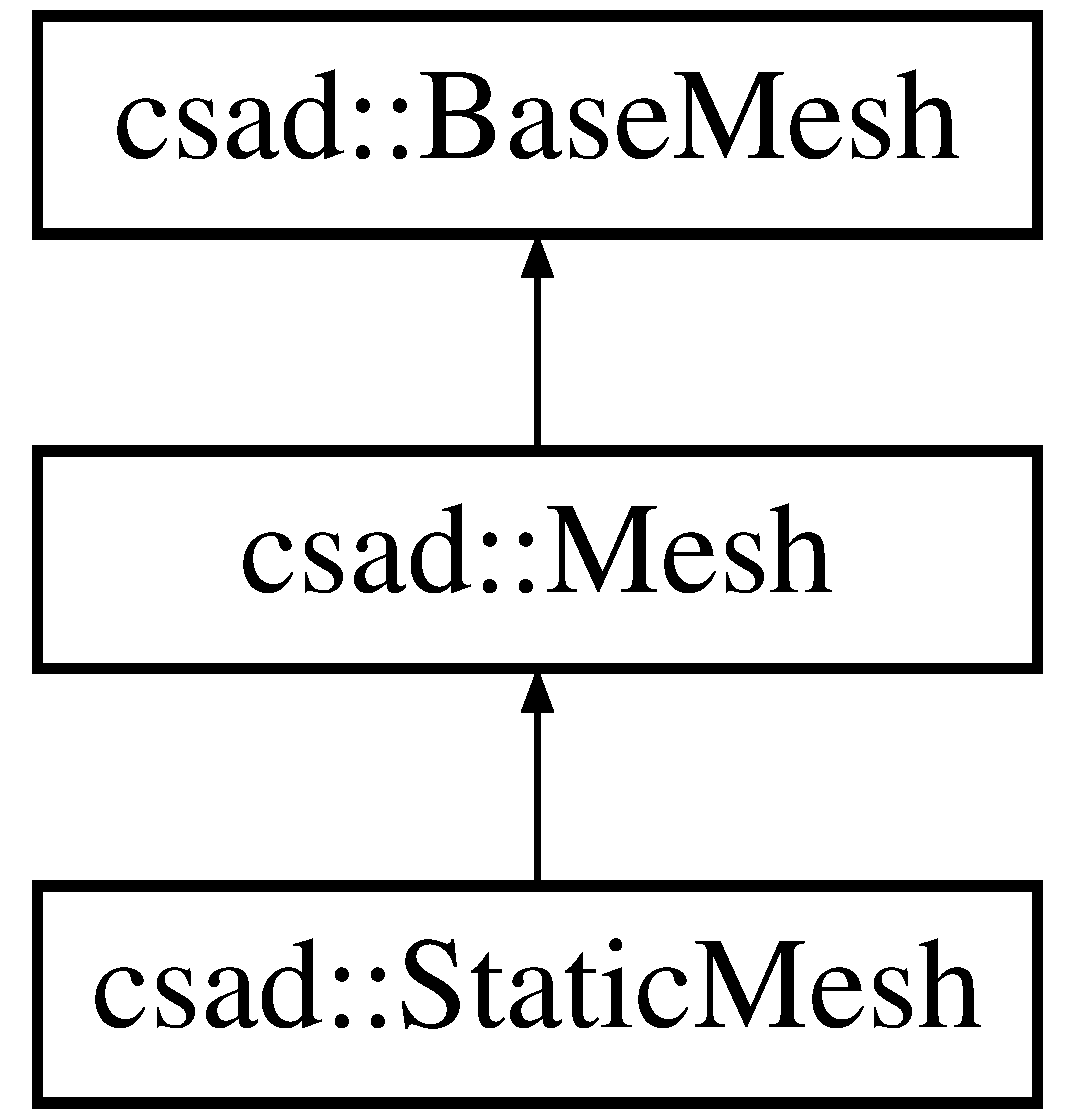
\includegraphics[height=3.000000cm]{classcsad_1_1_mesh}
\end{center}
\end{figure}
\subsection*{Public Types}
\begin{DoxyCompactItemize}
\item 
enum \hyperlink{classcsad_1_1_mesh_a0992cfc5c22b440ba3db818112d69caf}{st\-Draw\-Format} \{ \\*
\hyperlink{classcsad_1_1_mesh_a0992cfc5c22b440ba3db818112d69cafa3de5094fd0b896a96ac8843eb26372a6}{\-\_\-\-G\-L\-\_\-\-P\-O\-I\-N\-T\-S} = 0x000, 
\hyperlink{classcsad_1_1_mesh_a0992cfc5c22b440ba3db818112d69cafa96d7f461ff3cafed90a76e265f14000c}{\-\_\-\-G\-L\-\_\-\-L\-I\-N\-E\-S} = 0x001, 
\hyperlink{classcsad_1_1_mesh_a0992cfc5c22b440ba3db818112d69cafae346c44b2296dafed7e79abf41f2a6bc}{\-\_\-\-G\-L\-\_\-\-L\-I\-N\-E\-\_\-\-L\-O\-O\-P} = 0x002, 
\hyperlink{classcsad_1_1_mesh_a0992cfc5c22b440ba3db818112d69cafaea18fe065631e6702ceac01f9c155f5e}{\-\_\-\-G\-L\-\_\-\-L\-I\-N\-E\-\_\-\-S\-T\-R\-I\-P} = 0x003, 
\\*
\hyperlink{classcsad_1_1_mesh_a0992cfc5c22b440ba3db818112d69cafaa46b3b34e5ee3262e70765ca154f8cdb}{\-\_\-\-G\-L\-\_\-\-T\-R\-I\-A\-N\-G\-L\-E\-S} = 0x004, 
\hyperlink{classcsad_1_1_mesh_a0992cfc5c22b440ba3db818112d69cafae8f759bbd5014e890c1747b0da36c1f6}{\-\_\-\-G\-L\-\_\-\-T\-R\-I\-A\-N\-G\-L\-E\-\_\-\-S\-T\-R\-I\-P} = 0x005, 
\hyperlink{classcsad_1_1_mesh_a0992cfc5c22b440ba3db818112d69cafa8738be7b07f76a7973cc552a62848c4f}{\-\_\-\-G\-L\-\_\-\-T\-R\-I\-A\-N\-G\-L\-E\-\_\-\-F\-A\-N} = 0x006, 
\hyperlink{classcsad_1_1_mesh_a0992cfc5c22b440ba3db818112d69cafa7aaba1ec28c778d5791180cabd96f21b}{\-\_\-\-G\-L\-\_\-\-Q\-U\-A\-D\-S} = 0x007
, \\*
\hyperlink{classcsad_1_1_mesh_a0992cfc5c22b440ba3db818112d69cafa00abba265b60e709f6de1a7ba813cadc}{\-\_\-\-G\-L\-\_\-\-P\-O\-L\-Y\-G\-O\-N} = 0x009, 
\hyperlink{classcsad_1_1_mesh_a0992cfc5c22b440ba3db818112d69cafab4f067437253bdc27c8974215e82cb6d}{\-\_\-\-G\-L\-\_\-\-I\-N\-D\-E\-X\-\_\-\-B\-Y\-T\-E} = 0x01000000
, \hyperlink{classcsad_1_1_mesh_a0992cfc5c22b440ba3db818112d69cafa7d8084eacbd55804437eda4bc3fa056c}{\-\_\-\-G\-L\-\_\-\-N\-E\-E\-D\-\_\-\-I\-N\-D\-E\-X\-\_\-\-U\-P\-D\-A\-T\-E} = 0x10000000, 
\hyperlink{classcsad_1_1_mesh_a0992cfc5c22b440ba3db818112d69cafae5180995c07ee12224726847535634f7}{\-\_\-\-G\-L\-\_\-\-N\-E\-E\-D\-\_\-\-E\-L\-E\-M\-E\-N\-T\-\_\-\-U\-P\-D\-A\-T\-E} = 0x20000000
 \}
\begin{DoxyCompactList}\small\item\em the format of building geometry. \end{DoxyCompactList}\item 
enum \hyperlink{classcsad_1_1_mesh_acb32897739522133793f6cfe8564f780}{st\-Format} \{ \\*
\hyperlink{classcsad_1_1_mesh_acb32897739522133793f6cfe8564f780a5190f1b94505856d456f1d47d19deac6}{\-\_\-\-T\-G\-L\-\_\-\-V2\-F} = 0x00000001, 
\hyperlink{classcsad_1_1_mesh_acb32897739522133793f6cfe8564f780a5c0b3dcab62e79a2e6daa716f4dc7cd1}{\-\_\-\-T\-G\-L\-\_\-\-V3\-F} = 0x00000002
, \hyperlink{classcsad_1_1_mesh_acb32897739522133793f6cfe8564f780af221b582724c7091831ce91da22bc8f8}{\-\_\-\-T\-G\-L\-\_\-\-V2\-D} = 0x00000004, 
\hyperlink{classcsad_1_1_mesh_acb32897739522133793f6cfe8564f780ad47cabf22b9825c1f0ff6afa70a630ab}{\-\_\-\-T\-G\-L\-\_\-\-V3\-D} = 0x00000005
, \\*
\hyperlink{classcsad_1_1_mesh_acb32897739522133793f6cfe8564f780ae55d7cda49186c3c9e74990f82bb72a3}{\-\_\-\-T\-G\-L\-\_\-\-N3\-F} = 0x00000008, 
\hyperlink{classcsad_1_1_mesh_acb32897739522133793f6cfe8564f780a15428c085b8f3033148a9c2bc6e4db7a}{\-\_\-\-T\-G\-L\-\_\-0\-T1\-F} = 0x00000010, 
\hyperlink{classcsad_1_1_mesh_acb32897739522133793f6cfe8564f780a9214381484568ecba6f1048ff526649c}{\-\_\-\-T\-G\-L\-\_\-0\-T2\-F} = 0x00000020
, \hyperlink{classcsad_1_1_mesh_acb32897739522133793f6cfe8564f780a37d60c4a928dcc06f2b3d1fcf8e465b6}{\-\_\-\-T\-G\-L\-\_\-\-C3\-F} = 0x10000000, 
\\*
\hyperlink{classcsad_1_1_mesh_acb32897739522133793f6cfe8564f780a4bcd01e4a691dfdc1a12c5d170261c74}{\-\_\-\-T\-G\-L\-\_\-\-C4\-F} = 0x20000000
 \}
\begin{DoxyCompactList}\small\item\em the types of fields of geometry \end{DoxyCompactList}\item 
enum \hyperlink{classcsad_1_1_mesh_a3abde5863bf335c0575747d0d5761e19}{st\-Item} \{ \\*
\hyperlink{classcsad_1_1_mesh_a3abde5863bf335c0575747d0d5761e19a73bba428e4f7dade7f6961532116e7cf}{\-\_\-\-T\-E\-X\-T\-U\-R\-E0} = 0, 
\hyperlink{classcsad_1_1_mesh_a3abde5863bf335c0575747d0d5761e19aa5ddd01a77e8bc5ae9fa02e71ad30763}{\-\_\-\-T\-E\-X\-T\-U\-R\-E1} = 1, 
\hyperlink{classcsad_1_1_mesh_a3abde5863bf335c0575747d0d5761e19a74a1e5683692360cf0df911158ed27f2}{\-\_\-\-T\-E\-X\-T\-U\-R\-E2} = 2
, \hyperlink{classcsad_1_1_mesh_a3abde5863bf335c0575747d0d5761e19a627ddfa4a0e390500d46dd14f94527fa}{\-\_\-\-C\-O\-L\-O\-R} = 6, 
\\*
\hyperlink{classcsad_1_1_mesh_a3abde5863bf335c0575747d0d5761e19a80ab94ebc5c243bb96444d944fb36511}{\-\_\-\-N\-O\-R\-M\-A\-L} = 7, 
\hyperlink{classcsad_1_1_mesh_a3abde5863bf335c0575747d0d5761e19a306abe95d64e147789cdc1323895982c}{\-\_\-\-V\-E\-C\-T\-O\-R} = 8
 \}
\begin{DoxyCompactList}\small\item\em field vertex geometry. \end{DoxyCompactList}\end{DoxyCompactItemize}
\subsection*{Public Member Functions}
\begin{DoxyCompactItemize}
\item 
\hypertarget{classcsad_1_1_mesh_a2f2da578fdd319ce1840a76d6f20059b}{C\-S\-A\-D\-\_\-\-A\-P\-I \hyperlink{classbt_1_1vector3d}{vector3d} \hyperlink{classcsad_1_1_mesh_a2f2da578fdd319ce1840a76d6f20059b}{calculate\-Bound} ()}\label{classcsad_1_1_mesh_a2f2da578fdd319ce1840a76d6f20059b}

\begin{DoxyCompactList}\small\item\em preset sphere describing cube \end{DoxyCompactList}\item 
\hypertarget{classcsad_1_1_mesh_af4d2f34a11ddd431bb3e692a99fceb59}{C\-S\-A\-D\-\_\-\-A\-P\-I void \hyperlink{classcsad_1_1_mesh_af4d2f34a11ddd431bb3e692a99fceb59}{calculate\-Normals} ()}\label{classcsad_1_1_mesh_af4d2f34a11ddd431bb3e692a99fceb59}

\begin{DoxyCompactList}\small\item\em recalculate normals \end{DoxyCompactList}\item 
\hypertarget{classcsad_1_1_mesh_afb71bb61d549c453bea53ea03d20ce02}{C\-S\-A\-D\-\_\-\-A\-P\-I void \hyperlink{classcsad_1_1_mesh_afb71bb61d549c453bea53ea03d20ce02}{clean\-Index} (int from, int count)}\label{classcsad_1_1_mesh_afb71bb61d549c453bea53ea03d20ce02}

\begin{DoxyCompactList}\small\item\em specifies the zero index elements \end{DoxyCompactList}\item 
\hypertarget{classcsad_1_1_mesh_ac229d71ea69bea49ea15770ce6635d4b}{{\footnotesize template$<$typename T $>$ }\\\-\_\-\-F\-O\-R\-C\-E\-I\-N\-L\-I\-N\-E \hyperlink{classbt_1_1_link_array}{Link\-Array}$<$ T $>$ \hyperlink{classcsad_1_1_mesh_ac229d71ea69bea49ea15770ce6635d4b}{color} ()}\label{classcsad_1_1_mesh_ac229d71ea69bea49ea15770ce6635d4b}

\begin{DoxyCompactList}\small\item\em The array of vertices color. \end{DoxyCompactList}\item 
\hypertarget{classcsad_1_1_mesh_a3c75a7c40cb397153c55c38397056e75}{\-\_\-\-F\-O\-R\-C\-E\-I\-N\-L\-I\-N\-E unsigned char $\ast$\& \hyperlink{classcsad_1_1_mesh_a3c75a7c40cb397153c55c38397056e75}{elements} ()}\label{classcsad_1_1_mesh_a3c75a7c40cb397153c55c38397056e75}

\begin{DoxyCompactList}\small\item\em елементы геометрии \end{DoxyCompactList}\item 
\hypertarget{classcsad_1_1_mesh_accd0743abe213e3db30405443e69e149}{\-\_\-\-F\-O\-R\-C\-E\-I\-N\-L\-I\-N\-E unsigned int \hyperlink{classcsad_1_1_mesh_accd0743abe213e3db30405443e69e149}{elements\-Count} ()}\label{classcsad_1_1_mesh_accd0743abe213e3db30405443e69e149}

\begin{DoxyCompactList}\small\item\em returns the number of vertices \end{DoxyCompactList}\item 
\hypertarget{classcsad_1_1_mesh_a493f5dd55fd78c7cb80c1f53277e277d}{\-\_\-\-F\-O\-R\-C\-E\-I\-N\-L\-I\-N\-E unsigned int \hyperlink{classcsad_1_1_mesh_a493f5dd55fd78c7cb80c1f53277e277d}{element\-Size} ()}\label{classcsad_1_1_mesh_a493f5dd55fd78c7cb80c1f53277e277d}

\begin{DoxyCompactList}\small\item\em The size element. \end{DoxyCompactList}\item 
\hypertarget{classcsad_1_1_mesh_abe06cc3e046a6ae3d1bac6b166c2138d}{\-\_\-\-F\-O\-R\-C\-E\-I\-N\-L\-I\-N\-E \hyperlink{classbt_1_1vector4d}{vector4d} \& \hyperlink{classcsad_1_1_mesh_abe06cc3e046a6ae3d1bac6b166c2138d}{get\-Bound\-Sphere} ()}\label{classcsad_1_1_mesh_abe06cc3e046a6ae3d1bac6b166c2138d}

\begin{DoxyCompactList}\small\item\em returns a sector describing the cube in which pomeshaetsa geometry \end{DoxyCompactList}\item 
\hypertarget{classcsad_1_1_mesh_a76ec45b40a52b20976ac300fc1442b2d}{C\-S\-A\-D\-\_\-\-A\-P\-I unsigned int \hyperlink{classcsad_1_1_mesh_a76ec45b40a52b20976ac300fc1442b2d}{get\-Color\-Type} ()}\label{classcsad_1_1_mesh_a76ec45b40a52b20976ac300fc1442b2d}

\begin{DoxyCompactList}\small\item\em returns the color format of vertices\-: float\mbox{[}3\mbox{]} float\mbox{[}4\mbox{]} \end{DoxyCompactList}\item 
\hypertarget{classcsad_1_1_mesh_a92ec16d29adf1cb482510b6e9afec6af}{\-\_\-\-F\-O\-R\-C\-E\-I\-N\-L\-I\-N\-E \hyperlink{classcsad_1_1_mesh_a0992cfc5c22b440ba3db818112d69caf}{st\-Draw\-Format} \hyperlink{classcsad_1_1_mesh_a92ec16d29adf1cb482510b6e9afec6af}{get\-Draw\-Format} ()}\label{classcsad_1_1_mesh_a92ec16d29adf1cb482510b6e9afec6af}

\begin{DoxyCompactList}\small\item\em former rendering \end{DoxyCompactList}\item 
C\-S\-A\-D\-\_\-\-A\-P\-I unsigned int \hyperlink{classcsad_1_1_mesh_a9f243f44460f4de840b62b2101fdd370}{get\-Tex\-Type} (int id)
\item 
C\-S\-A\-D\-\_\-\-A\-P\-I unsigned int \hyperlink{classcsad_1_1_mesh_a283769e189167b4d4dfe32c0027e7485}{get\-Vector\-Type} ()
\item 
\hypertarget{classcsad_1_1_mesh_af203cd54a3c46b3c720405bfe8c01f3d}{{\footnotesize template$<$typename T $>$ }\\\-\_\-\-F\-O\-R\-C\-E\-I\-N\-L\-I\-N\-E \hyperlink{classbt_1_1_link_array}{Link\-Array}$<$ T $>$ \hyperlink{classcsad_1_1_mesh_af203cd54a3c46b3c720405bfe8c01f3d}{index} ()}\label{classcsad_1_1_mesh_af203cd54a3c46b3c720405bfe8c01f3d}

\begin{DoxyCompactList}\small\item\em Array indexes. \end{DoxyCompactList}\item 
\hypertarget{classcsad_1_1_mesh_a981d20a6176d6d185e19422746c5e086}{C\-S\-A\-D\-\_\-\-A\-P\-I int \hyperlink{classcsad_1_1_mesh_a981d20a6176d6d185e19422746c5e086}{index\-By\-Id} (unsigned int id)}\label{classcsad_1_1_mesh_a981d20a6176d6d185e19422746c5e086}

\begin{DoxyCompactList}\small\item\em value of index \end{DoxyCompactList}\item 
\hypertarget{classcsad_1_1_mesh_a71e46470010e0905fcfa50b915f17716}{\-\_\-\-F\-O\-R\-C\-E\-I\-N\-L\-I\-N\-E unsigned int \hyperlink{classcsad_1_1_mesh_a71e46470010e0905fcfa50b915f17716}{index\-Count} ()}\label{classcsad_1_1_mesh_a71e46470010e0905fcfa50b915f17716}

\begin{DoxyCompactList}\small\item\em returns the number of indexes \end{DoxyCompactList}\item 
\hypertarget{classcsad_1_1_mesh_a349384032c4f2c6dca94d5db2bf09244}{C\-S\-A\-D\-\_\-\-A\-P\-I bool \hyperlink{classcsad_1_1_mesh_a349384032c4f2c6dca94d5db2bf09244}{is\-Normal} ()}\label{classcsad_1_1_mesh_a349384032c4f2c6dca94d5db2bf09244}

\begin{DoxyCompactList}\small\item\em returns true if the vertices contains the vector of the front \end{DoxyCompactList}\item 
\hypertarget{classcsad_1_1_mesh_a318ef5aa68a31189edcbb88c86c53d11}{{\footnotesize template$<$typename T $>$ }\\\-\_\-\-F\-O\-R\-C\-E\-I\-N\-L\-I\-N\-E \hyperlink{classbt_1_1_link_array}{Link\-Array}$<$ T $>$ \hyperlink{classcsad_1_1_mesh_a318ef5aa68a31189edcbb88c86c53d11}{normal} ()}\label{classcsad_1_1_mesh_a318ef5aa68a31189edcbb88c86c53d11}

\begin{DoxyCompactList}\small\item\em Array normals. \end{DoxyCompactList}\item 
\hypertarget{classcsad_1_1_mesh_aed3508dc678922784b993b5d0f9f3d7e}{C\-S\-A\-D\-\_\-\-A\-P\-I \hyperlink{classcsad_1_1_mesh}{Mesh} \& \hyperlink{classcsad_1_1_mesh_aed3508dc678922784b993b5d0f9f3d7e}{resize\-Index} (unsigned int count)}\label{classcsad_1_1_mesh_aed3508dc678922784b993b5d0f9f3d7e}

\begin{DoxyCompactList}\small\item\em Changes the number of indexes, preserving the values at the end of the array. \end{DoxyCompactList}\item 
\hypertarget{classcsad_1_1_mesh_ac085ab6ad1014f2b95bc0da85997cf8b}{C\-S\-A\-D\-\_\-\-A\-P\-I \hyperlink{classcsad_1_1_mesh}{Mesh} \& \hyperlink{classcsad_1_1_mesh_ac085ab6ad1014f2b95bc0da85997cf8b}{resize\-Vertex} (unsigned int count)}\label{classcsad_1_1_mesh_ac085ab6ad1014f2b95bc0da85997cf8b}

\begin{DoxyCompactList}\small\item\em Changes the number of elements, preserving the values at the end of the array. \end{DoxyCompactList}\item 
\hypertarget{classcsad_1_1_mesh_a70f83064ff22715e6a0ae5f4894472c2}{C\-S\-A\-D\-\_\-\-A\-P\-I \hyperlink{classcsad_1_1_mesh}{Mesh} \& \hyperlink{classcsad_1_1_mesh_a70f83064ff22715e6a0ae5f4894472c2}{set\-Draw\-Format} (\hyperlink{classcsad_1_1_mesh_a0992cfc5c22b440ba3db818112d69caf}{st\-Draw\-Format} attr)}\label{classcsad_1_1_mesh_a70f83064ff22715e6a0ae5f4894472c2}

\begin{DoxyCompactList}\small\item\em задает тип геометри \end{DoxyCompactList}\item 
\hypertarget{classcsad_1_1_mesh_afba476289c0dc2a0e3c382cc1eceba99}{C\-S\-A\-D\-\_\-\-A\-P\-I \hyperlink{classcsad_1_1_mesh}{Mesh} \& \hyperlink{classcsad_1_1_mesh_afba476289c0dc2a0e3c382cc1eceba99}{set\-Fields} (unsigned int attr)}\label{classcsad_1_1_mesh_afba476289c0dc2a0e3c382cc1eceba99}

\begin{DoxyCompactList}\small\item\em to install the vertex format \end{DoxyCompactList}\item 
\hypertarget{classcsad_1_1_mesh_a728eb98e02ca5cf2eb122ef63aca4c95}{C\-S\-A\-D\-\_\-\-A\-P\-I \hyperlink{classcsad_1_1_mesh}{Mesh} \& \hyperlink{classcsad_1_1_mesh_a728eb98e02ca5cf2eb122ef63aca4c95}{set\-Index} (unsigned int i, int val)}\label{classcsad_1_1_mesh_a728eb98e02ca5cf2eb122ef63aca4c95}

\begin{DoxyCompactList}\small\item\em installing index \end{DoxyCompactList}\item 
\hypertarget{classcsad_1_1_mesh_a87c8755460e51fce2b7fcd544c17e07f}{C\-S\-A\-D\-\_\-\-A\-P\-I \hyperlink{classcsad_1_1_mesh}{Mesh} \& \hyperlink{classcsad_1_1_mesh_a87c8755460e51fce2b7fcd544c17e07f}{set\-Index\-Count} (unsigned int count)}\label{classcsad_1_1_mesh_a87c8755460e51fce2b7fcd544c17e07f}

\begin{DoxyCompactList}\small\item\em Sets the number of indexes, the previous value of the index is not saved. \end{DoxyCompactList}\item 
\hypertarget{classcsad_1_1_mesh_a40e58b4af7cf86102765ada030b0b647}{C\-S\-A\-D\-\_\-\-A\-P\-I \hyperlink{classcsad_1_1_mesh}{Mesh} \& \hyperlink{classcsad_1_1_mesh_a40e58b4af7cf86102765ada030b0b647}{set\-Index\-Line} (unsigned int i, unsigned int a, unsigned int b)}\label{classcsad_1_1_mesh_a40e58b4af7cf86102765ada030b0b647}

\begin{DoxyCompactList}\small\item\em installation of two indexess in a row \end{DoxyCompactList}\item 
\hypertarget{classcsad_1_1_mesh_a6964f6d0e3a982a210741bdc8b415346}{C\-S\-A\-D\-\_\-\-A\-P\-I \hyperlink{classcsad_1_1_mesh}{Mesh} \& \hyperlink{classcsad_1_1_mesh_a6964f6d0e3a982a210741bdc8b415346}{set\-Index\-Quad} (unsigned int i, unsigned int a, unsigned int b, unsigned int c, unsigned int d)}\label{classcsad_1_1_mesh_a6964f6d0e3a982a210741bdc8b415346}

\begin{DoxyCompactList}\small\item\em installation of four indexes in a row \end{DoxyCompactList}\item 
\hypertarget{classcsad_1_1_mesh_add0ee563d6adea5c387f8ac66e03a38b}{C\-S\-A\-D\-\_\-\-A\-P\-I \hyperlink{classcsad_1_1_mesh}{Mesh} \& \hyperlink{classcsad_1_1_mesh_add0ee563d6adea5c387f8ac66e03a38b}{set\-Index\-Tri} (unsigned int i, unsigned int a, unsigned int b, unsigned int c)}\label{classcsad_1_1_mesh_add0ee563d6adea5c387f8ac66e03a38b}

\begin{DoxyCompactList}\small\item\em installation of three indexes in a row \end{DoxyCompactList}\item 
\hypertarget{classcsad_1_1_mesh_a698ca8b4ed067aeffe7fc51ae7fc580d}{C\-S\-A\-D\-\_\-\-A\-P\-I \hyperlink{classcsad_1_1_mesh}{Mesh} \& \hyperlink{classcsad_1_1_mesh_a698ca8b4ed067aeffe7fc51ae7fc580d}{set\-Vector} (unsigned int i, float $\ast$v)}\label{classcsad_1_1_mesh_a698ca8b4ed067aeffe7fc51ae7fc580d}

\begin{DoxyCompactList}\small\item\em slow installation vertix \end{DoxyCompactList}\item 
\hypertarget{classcsad_1_1_mesh_a7a523d5df0fb192fd5f8f88b3522a7d7}{C\-S\-A\-D\-\_\-\-A\-P\-I \hyperlink{classcsad_1_1_mesh}{Mesh} \& \hyperlink{classcsad_1_1_mesh_a7a523d5df0fb192fd5f8f88b3522a7d7}{set\-Vector} (unsigned int i, double $\ast$v)}\label{classcsad_1_1_mesh_a7a523d5df0fb192fd5f8f88b3522a7d7}

\begin{DoxyCompactList}\small\item\em slow installation vertix \end{DoxyCompactList}\item 
\hypertarget{classcsad_1_1_mesh_a7204425ae77e50f52a019acb8c566e8f}{C\-S\-A\-D\-\_\-\-A\-P\-I \hyperlink{classcsad_1_1_mesh}{Mesh} \& \hyperlink{classcsad_1_1_mesh_a7204425ae77e50f52a019acb8c566e8f}{set\-Vertex\-Count} (unsigned int count)}\label{classcsad_1_1_mesh_a7204425ae77e50f52a019acb8c566e8f}

\begin{DoxyCompactList}\small\item\em Sets the number of elements vertex buffer, the previous value of vertices is not saved. \end{DoxyCompactList}\item 
\hypertarget{classcsad_1_1_mesh_a2225a16afadd8f40884ca478a90046f8}{{\footnotesize template$<$typename T $>$ }\\\-\_\-\-F\-O\-R\-C\-E\-I\-N\-L\-I\-N\-E \hyperlink{classbt_1_1_link_array}{Link\-Array}$<$ T $>$ \hyperlink{classcsad_1_1_mesh_a2225a16afadd8f40884ca478a90046f8}{texture0} ()}\label{classcsad_1_1_mesh_a2225a16afadd8f40884ca478a90046f8}

\begin{DoxyCompactList}\small\item\em An array of texture coordinates. \end{DoxyCompactList}\item 
\hypertarget{classcsad_1_1_mesh_abe780b944ddb3c807305cfba8adfe5e1}{{\footnotesize template$<$typename T $>$ }\\\-\_\-\-F\-O\-R\-C\-E\-I\-N\-L\-I\-N\-E \hyperlink{classbt_1_1_link_array}{Link\-Array}$<$ T $>$ \hyperlink{classcsad_1_1_mesh_abe780b944ddb3c807305cfba8adfe5e1}{texture1} ()}\label{classcsad_1_1_mesh_abe780b944ddb3c807305cfba8adfe5e1}

\begin{DoxyCompactList}\small\item\em An array of texture coordinates. \end{DoxyCompactList}\item 
\hypertarget{classcsad_1_1_mesh_ad6361e5eabad983a785dc4503ba623dd}{\-\_\-\-F\-O\-R\-C\-E\-I\-N\-L\-I\-N\-E void \hyperlink{classcsad_1_1_mesh_ad6361e5eabad983a785dc4503ba623dd}{update} ()}\label{classcsad_1_1_mesh_ad6361e5eabad983a785dc4503ba623dd}

\begin{DoxyCompactList}\small\item\em the next drawing geometry updated on the device \end{DoxyCompactList}\item 
\hypertarget{classcsad_1_1_mesh_a44c3c64d768c4dd56e58eab5b88e65c1}{\-\_\-\-F\-O\-R\-C\-E\-I\-N\-L\-I\-N\-E void \hyperlink{classcsad_1_1_mesh_a44c3c64d768c4dd56e58eab5b88e65c1}{update\-Vertex} ()}\label{classcsad_1_1_mesh_a44c3c64d768c4dd56e58eab5b88e65c1}

\begin{DoxyCompactList}\small\item\em the next drawing vertex geometry updated on the device \end{DoxyCompactList}\item 
\hypertarget{classcsad_1_1_mesh_aa010612b3a0b8f331d97505e45d8353a}{{\footnotesize template$<$typename T $>$ }\\\-\_\-\-F\-O\-R\-C\-E\-I\-N\-L\-I\-N\-E \hyperlink{classbt_1_1_link_array}{Link\-Array}$<$ T $>$ \hyperlink{classcsad_1_1_mesh_aa010612b3a0b8f331d97505e45d8353a}{vector} ()}\label{classcsad_1_1_mesh_aa010612b3a0b8f331d97505e45d8353a}

\begin{DoxyCompactList}\small\item\em The array of vertices positions. \end{DoxyCompactList}\item 
\hypertarget{classcsad_1_1_mesh_aeaadb3131f721f29fd0b7dfdc4e10be8}{{\footnotesize template$<$typename T $>$ }\\\-\_\-\-F\-O\-R\-C\-E\-I\-N\-L\-I\-N\-E \hyperlink{classbt_1_1_link_array}{Link\-Array}$<$ T $>$ \hyperlink{classcsad_1_1_mesh_aeaadb3131f721f29fd0b7dfdc4e10be8}{vertex} ()}\label{classcsad_1_1_mesh_aeaadb3131f721f29fd0b7dfdc4e10be8}

\begin{DoxyCompactList}\small\item\em The array of vertices. \end{DoxyCompactList}\end{DoxyCompactItemize}
\subsection*{Static Public Attributes}
\begin{DoxyCompactItemize}
\item 
\hypertarget{classcsad_1_1_mesh_a4182d08a8d02d924319ab10c3e3c850d}{static C\-S\-A\-D\-\_\-\-A\-P\-I \hyperlink{classcsad_1_1_mesh}{Mesh} $\ast$ \hyperlink{classcsad_1_1_mesh_a4182d08a8d02d924319ab10c3e3c850d}{Cube}}\label{classcsad_1_1_mesh_a4182d08a8d02d924319ab10c3e3c850d}

\begin{DoxyCompactList}\small\item\em Геометрия куба \end{DoxyCompactList}\item 
\hypertarget{classcsad_1_1_mesh_a6f4b2f018b6ac1ad03f75f0cd7e7398e}{static C\-S\-A\-D\-\_\-\-A\-P\-I \hyperlink{classcsad_1_1_mesh}{Mesh} $\ast$ \hyperlink{classcsad_1_1_mesh_a6f4b2f018b6ac1ad03f75f0cd7e7398e}{Quad}}\label{classcsad_1_1_mesh_a6f4b2f018b6ac1ad03f75f0cd7e7398e}

\begin{DoxyCompactList}\small\item\em Геометрия квадрата \end{DoxyCompactList}\end{DoxyCompactItemize}
\subsection*{Friends}
\begin{DoxyCompactItemize}
\item 
\hypertarget{classcsad_1_1_mesh_a7a0fd97956d115f48a68405a7feed6db}{class {\bfseries gen\-::\-Modeller\-Mesh}}\label{classcsad_1_1_mesh_a7a0fd97956d115f48a68405a7feed6db}

\end{DoxyCompactItemize}


\subsection{Detailed Description}
\hyperlink{classcsad_1_1_mesh}{Mesh} -\/ geometric container sets vertex model object. Tops in its composition can have the following characteristics\-: position, color, vector front, texture coordinates. 

\begin{DoxySeeAlso}{See Also}
\hyperlink{group__scene}{csad\-: scene} \hyperlink{classcsad_1_1_mesh_filter}{Mesh\-Filter} \hyperlink{classcsad_1_1_static_mesh}{Static\-Mesh} \hyperlink{classcsad_1_1_v_b_o_mesh}{V\-B\-O\-Mesh} 
\end{DoxySeeAlso}


\subsection{Member Enumeration Documentation}
\hypertarget{classcsad_1_1_mesh_a0992cfc5c22b440ba3db818112d69caf}{\index{csad\-::\-Mesh@{csad\-::\-Mesh}!st\-Draw\-Format@{st\-Draw\-Format}}
\index{st\-Draw\-Format@{st\-Draw\-Format}!csad::Mesh@{csad\-::\-Mesh}}
\subsubsection[{st\-Draw\-Format}]{\setlength{\rightskip}{0pt plus 5cm}enum {\bf csad\-::\-Mesh\-::st\-Draw\-Format}}}\label{classcsad_1_1_mesh_a0992cfc5c22b440ba3db818112d69caf}


the format of building geometry. 

\begin{Desc}
\item[Enumerator]\par
\begin{description}
\index{\-\_\-\-G\-L\-\_\-\-P\-O\-I\-N\-T\-S@{\-\_\-\-G\-L\-\_\-\-P\-O\-I\-N\-T\-S}!csad\-::\-Mesh@{csad\-::\-Mesh}}\index{csad\-::\-Mesh@{csad\-::\-Mesh}!\-\_\-\-G\-L\-\_\-\-P\-O\-I\-N\-T\-S@{\-\_\-\-G\-L\-\_\-\-P\-O\-I\-N\-T\-S}}\item[{\em 
\hypertarget{classcsad_1_1_mesh_a0992cfc5c22b440ba3db818112d69cafa3de5094fd0b896a96ac8843eb26372a6}{\-\_\-\-G\-L\-\_\-\-P\-O\-I\-N\-T\-S}\label{classcsad_1_1_mesh_a0992cfc5c22b440ba3db818112d69cafa3de5094fd0b896a96ac8843eb26372a6}
}]вершина интерпретируется как отдельная точка. \index{\-\_\-\-G\-L\-\_\-\-L\-I\-N\-E\-S@{\-\_\-\-G\-L\-\_\-\-L\-I\-N\-E\-S}!csad\-::\-Mesh@{csad\-::\-Mesh}}\index{csad\-::\-Mesh@{csad\-::\-Mesh}!\-\_\-\-G\-L\-\_\-\-L\-I\-N\-E\-S@{\-\_\-\-G\-L\-\_\-\-L\-I\-N\-E\-S}}\item[{\em 
\hypertarget{classcsad_1_1_mesh_a0992cfc5c22b440ba3db818112d69cafa96d7f461ff3cafed90a76e265f14000c}{\-\_\-\-G\-L\-\_\-\-L\-I\-N\-E\-S}\label{classcsad_1_1_mesh_a0992cfc5c22b440ba3db818112d69cafa96d7f461ff3cafed90a76e265f14000c}
}]пара вершин интерпретируются как линия. \index{\-\_\-\-G\-L\-\_\-\-L\-I\-N\-E\-\_\-\-L\-O\-O\-P@{\-\_\-\-G\-L\-\_\-\-L\-I\-N\-E\-\_\-\-L\-O\-O\-P}!csad\-::\-Mesh@{csad\-::\-Mesh}}\index{csad\-::\-Mesh@{csad\-::\-Mesh}!\-\_\-\-G\-L\-\_\-\-L\-I\-N\-E\-\_\-\-L\-O\-O\-P@{\-\_\-\-G\-L\-\_\-\-L\-I\-N\-E\-\_\-\-L\-O\-O\-P}}\item[{\em 
\hypertarget{classcsad_1_1_mesh_a0992cfc5c22b440ba3db818112d69cafae346c44b2296dafed7e79abf41f2a6bc}{\-\_\-\-G\-L\-\_\-\-L\-I\-N\-E\-\_\-\-L\-O\-O\-P}\label{classcsad_1_1_mesh_a0992cfc5c22b440ba3db818112d69cafae346c44b2296dafed7e79abf41f2a6bc}
}]каждая вершина участвует в построении замкнутой линейной фигуры. \index{\-\_\-\-G\-L\-\_\-\-L\-I\-N\-E\-\_\-\-S\-T\-R\-I\-P@{\-\_\-\-G\-L\-\_\-\-L\-I\-N\-E\-\_\-\-S\-T\-R\-I\-P}!csad\-::\-Mesh@{csad\-::\-Mesh}}\index{csad\-::\-Mesh@{csad\-::\-Mesh}!\-\_\-\-G\-L\-\_\-\-L\-I\-N\-E\-\_\-\-S\-T\-R\-I\-P@{\-\_\-\-G\-L\-\_\-\-L\-I\-N\-E\-\_\-\-S\-T\-R\-I\-P}}\item[{\em 
\hypertarget{classcsad_1_1_mesh_a0992cfc5c22b440ba3db818112d69cafaea18fe065631e6702ceac01f9c155f5e}{\-\_\-\-G\-L\-\_\-\-L\-I\-N\-E\-\_\-\-S\-T\-R\-I\-P}\label{classcsad_1_1_mesh_a0992cfc5c22b440ba3db818112d69cafaea18fe065631e6702ceac01f9c155f5e}
}]каждая вершина участвует в построении не замкнутой линейной фигуры. \index{\-\_\-\-G\-L\-\_\-\-T\-R\-I\-A\-N\-G\-L\-E\-S@{\-\_\-\-G\-L\-\_\-\-T\-R\-I\-A\-N\-G\-L\-E\-S}!csad\-::\-Mesh@{csad\-::\-Mesh}}\index{csad\-::\-Mesh@{csad\-::\-Mesh}!\-\_\-\-G\-L\-\_\-\-T\-R\-I\-A\-N\-G\-L\-E\-S@{\-\_\-\-G\-L\-\_\-\-T\-R\-I\-A\-N\-G\-L\-E\-S}}\item[{\em 
\hypertarget{classcsad_1_1_mesh_a0992cfc5c22b440ba3db818112d69cafaa46b3b34e5ee3262e70765ca154f8cdb}{\-\_\-\-G\-L\-\_\-\-T\-R\-I\-A\-N\-G\-L\-E\-S}\label{classcsad_1_1_mesh_a0992cfc5c22b440ba3db818112d69cafaa46b3b34e5ee3262e70765ca154f8cdb}
}]каждые три вершины задают треугольник. \index{\-\_\-\-G\-L\-\_\-\-T\-R\-I\-A\-N\-G\-L\-E\-\_\-\-S\-T\-R\-I\-P@{\-\_\-\-G\-L\-\_\-\-T\-R\-I\-A\-N\-G\-L\-E\-\_\-\-S\-T\-R\-I\-P}!csad\-::\-Mesh@{csad\-::\-Mesh}}\index{csad\-::\-Mesh@{csad\-::\-Mesh}!\-\_\-\-G\-L\-\_\-\-T\-R\-I\-A\-N\-G\-L\-E\-\_\-\-S\-T\-R\-I\-P@{\-\_\-\-G\-L\-\_\-\-T\-R\-I\-A\-N\-G\-L\-E\-\_\-\-S\-T\-R\-I\-P}}\item[{\em 
\hypertarget{classcsad_1_1_mesh_a0992cfc5c22b440ba3db818112d69cafae8f759bbd5014e890c1747b0da36c1f6}{\-\_\-\-G\-L\-\_\-\-T\-R\-I\-A\-N\-G\-L\-E\-\_\-\-S\-T\-R\-I\-P}\label{classcsad_1_1_mesh_a0992cfc5c22b440ba3db818112d69cafae8f759bbd5014e890c1747b0da36c1f6}
}]треугольник производится из двух предыдущий вершин и текущей. \index{\-\_\-\-G\-L\-\_\-\-T\-R\-I\-A\-N\-G\-L\-E\-\_\-\-F\-A\-N@{\-\_\-\-G\-L\-\_\-\-T\-R\-I\-A\-N\-G\-L\-E\-\_\-\-F\-A\-N}!csad\-::\-Mesh@{csad\-::\-Mesh}}\index{csad\-::\-Mesh@{csad\-::\-Mesh}!\-\_\-\-G\-L\-\_\-\-T\-R\-I\-A\-N\-G\-L\-E\-\_\-\-F\-A\-N@{\-\_\-\-G\-L\-\_\-\-T\-R\-I\-A\-N\-G\-L\-E\-\_\-\-F\-A\-N}}\item[{\em 
\hypertarget{classcsad_1_1_mesh_a0992cfc5c22b440ba3db818112d69cafa8738be7b07f76a7973cc552a62848c4f}{\-\_\-\-G\-L\-\_\-\-T\-R\-I\-A\-N\-G\-L\-E\-\_\-\-F\-A\-N}\label{classcsad_1_1_mesh_a0992cfc5c22b440ba3db818112d69cafa8738be7b07f76a7973cc552a62848c4f}
}]каждая вершина строит треугольник к предыдущей грани треугольника или первой пары вершин, все треугольники имеют общую первую вершину. \index{\-\_\-\-G\-L\-\_\-\-Q\-U\-A\-D\-S@{\-\_\-\-G\-L\-\_\-\-Q\-U\-A\-D\-S}!csad\-::\-Mesh@{csad\-::\-Mesh}}\index{csad\-::\-Mesh@{csad\-::\-Mesh}!\-\_\-\-G\-L\-\_\-\-Q\-U\-A\-D\-S@{\-\_\-\-G\-L\-\_\-\-Q\-U\-A\-D\-S}}\item[{\em 
\hypertarget{classcsad_1_1_mesh_a0992cfc5c22b440ba3db818112d69cafa7aaba1ec28c778d5791180cabd96f21b}{\-\_\-\-G\-L\-\_\-\-Q\-U\-A\-D\-S}\label{classcsad_1_1_mesh_a0992cfc5c22b440ba3db818112d69cafa7aaba1ec28c778d5791180cabd96f21b}
}]каждые четыре вершины задают пару смежных треугольников. \index{\-\_\-\-G\-L\-\_\-\-P\-O\-L\-Y\-G\-O\-N@{\-\_\-\-G\-L\-\_\-\-P\-O\-L\-Y\-G\-O\-N}!csad\-::\-Mesh@{csad\-::\-Mesh}}\index{csad\-::\-Mesh@{csad\-::\-Mesh}!\-\_\-\-G\-L\-\_\-\-P\-O\-L\-Y\-G\-O\-N@{\-\_\-\-G\-L\-\_\-\-P\-O\-L\-Y\-G\-O\-N}}\item[{\em 
\hypertarget{classcsad_1_1_mesh_a0992cfc5c22b440ba3db818112d69cafa00abba265b60e709f6de1a7ba813cadc}{\-\_\-\-G\-L\-\_\-\-P\-O\-L\-Y\-G\-O\-N}\label{classcsad_1_1_mesh_a0992cfc5c22b440ba3db818112d69cafa00abba265b60e709f6de1a7ba813cadc}
}]замкнутый полигон разделяется индексами -\/1. \index{\-\_\-\-G\-L\-\_\-\-I\-N\-D\-E\-X\-\_\-\-B\-Y\-T\-E@{\-\_\-\-G\-L\-\_\-\-I\-N\-D\-E\-X\-\_\-\-B\-Y\-T\-E}!csad\-::\-Mesh@{csad\-::\-Mesh}}\index{csad\-::\-Mesh@{csad\-::\-Mesh}!\-\_\-\-G\-L\-\_\-\-I\-N\-D\-E\-X\-\_\-\-B\-Y\-T\-E@{\-\_\-\-G\-L\-\_\-\-I\-N\-D\-E\-X\-\_\-\-B\-Y\-T\-E}}\item[{\em 
\hypertarget{classcsad_1_1_mesh_a0992cfc5c22b440ba3db818112d69cafab4f067437253bdc27c8974215e82cb6d}{\-\_\-\-G\-L\-\_\-\-I\-N\-D\-E\-X\-\_\-\-B\-Y\-T\-E}\label{classcsad_1_1_mesh_a0992cfc5c22b440ba3db818112d69cafab4f067437253bdc27c8974215e82cb6d}
}]gl\-Index\-Size \index{\-\_\-\-G\-L\-\_\-\-N\-E\-E\-D\-\_\-\-I\-N\-D\-E\-X\-\_\-\-U\-P\-D\-A\-T\-E@{\-\_\-\-G\-L\-\_\-\-N\-E\-E\-D\-\_\-\-I\-N\-D\-E\-X\-\_\-\-U\-P\-D\-A\-T\-E}!csad\-::\-Mesh@{csad\-::\-Mesh}}\index{csad\-::\-Mesh@{csad\-::\-Mesh}!\-\_\-\-G\-L\-\_\-\-N\-E\-E\-D\-\_\-\-I\-N\-D\-E\-X\-\_\-\-U\-P\-D\-A\-T\-E@{\-\_\-\-G\-L\-\_\-\-N\-E\-E\-D\-\_\-\-I\-N\-D\-E\-X\-\_\-\-U\-P\-D\-A\-T\-E}}\item[{\em 
\hypertarget{classcsad_1_1_mesh_a0992cfc5c22b440ba3db818112d69cafa7d8084eacbd55804437eda4bc3fa056c}{\-\_\-\-G\-L\-\_\-\-N\-E\-E\-D\-\_\-\-I\-N\-D\-E\-X\-\_\-\-U\-P\-D\-A\-T\-E}\label{classcsad_1_1_mesh_a0992cfc5c22b440ba3db818112d69cafa7d8084eacbd55804437eda4bc3fa056c}
}]буфер индекса требует обновления на устройстве \index{\-\_\-\-G\-L\-\_\-\-N\-E\-E\-D\-\_\-\-E\-L\-E\-M\-E\-N\-T\-\_\-\-U\-P\-D\-A\-T\-E@{\-\_\-\-G\-L\-\_\-\-N\-E\-E\-D\-\_\-\-E\-L\-E\-M\-E\-N\-T\-\_\-\-U\-P\-D\-A\-T\-E}!csad\-::\-Mesh@{csad\-::\-Mesh}}\index{csad\-::\-Mesh@{csad\-::\-Mesh}!\-\_\-\-G\-L\-\_\-\-N\-E\-E\-D\-\_\-\-E\-L\-E\-M\-E\-N\-T\-\_\-\-U\-P\-D\-A\-T\-E@{\-\_\-\-G\-L\-\_\-\-N\-E\-E\-D\-\_\-\-E\-L\-E\-M\-E\-N\-T\-\_\-\-U\-P\-D\-A\-T\-E}}\item[{\em 
\hypertarget{classcsad_1_1_mesh_a0992cfc5c22b440ba3db818112d69cafae5180995c07ee12224726847535634f7}{\-\_\-\-G\-L\-\_\-\-N\-E\-E\-D\-\_\-\-E\-L\-E\-M\-E\-N\-T\-\_\-\-U\-P\-D\-A\-T\-E}\label{classcsad_1_1_mesh_a0992cfc5c22b440ba3db818112d69cafae5180995c07ee12224726847535634f7}
}]буфер вершин требует обновления на устройстве \end{description}
\end{Desc}
\hypertarget{classcsad_1_1_mesh_acb32897739522133793f6cfe8564f780}{\index{csad\-::\-Mesh@{csad\-::\-Mesh}!st\-Format@{st\-Format}}
\index{st\-Format@{st\-Format}!csad::Mesh@{csad\-::\-Mesh}}
\subsubsection[{st\-Format}]{\setlength{\rightskip}{0pt plus 5cm}enum {\bf csad\-::\-Mesh\-::st\-Format}}}\label{classcsad_1_1_mesh_acb32897739522133793f6cfe8564f780}


the types of fields of geometry 

\begin{Desc}
\item[Enumerator]\par
\begin{description}
\index{\-\_\-\-T\-G\-L\-\_\-\-V2\-F@{\-\_\-\-T\-G\-L\-\_\-\-V2\-F}!csad\-::\-Mesh@{csad\-::\-Mesh}}\index{csad\-::\-Mesh@{csad\-::\-Mesh}!\-\_\-\-T\-G\-L\-\_\-\-V2\-F@{\-\_\-\-T\-G\-L\-\_\-\-V2\-F}}\item[{\em 
\hypertarget{classcsad_1_1_mesh_acb32897739522133793f6cfe8564f780a5190f1b94505856d456f1d47d19deac6}{\-\_\-\-T\-G\-L\-\_\-\-V2\-F}\label{classcsad_1_1_mesh_acb32897739522133793f6cfe8564f780a5190f1b94505856d456f1d47d19deac6}
}]two-\/dimensional coordinates single-\/precision \index{\-\_\-\-T\-G\-L\-\_\-\-V3\-F@{\-\_\-\-T\-G\-L\-\_\-\-V3\-F}!csad\-::\-Mesh@{csad\-::\-Mesh}}\index{csad\-::\-Mesh@{csad\-::\-Mesh}!\-\_\-\-T\-G\-L\-\_\-\-V3\-F@{\-\_\-\-T\-G\-L\-\_\-\-V3\-F}}\item[{\em 
\hypertarget{classcsad_1_1_mesh_acb32897739522133793f6cfe8564f780a5c0b3dcab62e79a2e6daa716f4dc7cd1}{\-\_\-\-T\-G\-L\-\_\-\-V3\-F}\label{classcsad_1_1_mesh_acb32897739522133793f6cfe8564f780a5c0b3dcab62e79a2e6daa716f4dc7cd1}
}]three-\/dimensional coordinates of single-\/precision \index{\-\_\-\-T\-G\-L\-\_\-\-V2\-D@{\-\_\-\-T\-G\-L\-\_\-\-V2\-D}!csad\-::\-Mesh@{csad\-::\-Mesh}}\index{csad\-::\-Mesh@{csad\-::\-Mesh}!\-\_\-\-T\-G\-L\-\_\-\-V2\-D@{\-\_\-\-T\-G\-L\-\_\-\-V2\-D}}\item[{\em 
\hypertarget{classcsad_1_1_mesh_acb32897739522133793f6cfe8564f780af221b582724c7091831ce91da22bc8f8}{\-\_\-\-T\-G\-L\-\_\-\-V2\-D}\label{classcsad_1_1_mesh_acb32897739522133793f6cfe8564f780af221b582724c7091831ce91da22bc8f8}
}]two-\/dimensional double-\/precision coordinates \index{\-\_\-\-T\-G\-L\-\_\-\-V3\-D@{\-\_\-\-T\-G\-L\-\_\-\-V3\-D}!csad\-::\-Mesh@{csad\-::\-Mesh}}\index{csad\-::\-Mesh@{csad\-::\-Mesh}!\-\_\-\-T\-G\-L\-\_\-\-V3\-D@{\-\_\-\-T\-G\-L\-\_\-\-V3\-D}}\item[{\em 
\hypertarget{classcsad_1_1_mesh_acb32897739522133793f6cfe8564f780ad47cabf22b9825c1f0ff6afa70a630ab}{\-\_\-\-T\-G\-L\-\_\-\-V3\-D}\label{classcsad_1_1_mesh_acb32897739522133793f6cfe8564f780ad47cabf22b9825c1f0ff6afa70a630ab}
}]three-\/dimensional double-\/precision coordinates \index{\-\_\-\-T\-G\-L\-\_\-\-N3\-F@{\-\_\-\-T\-G\-L\-\_\-\-N3\-F}!csad\-::\-Mesh@{csad\-::\-Mesh}}\index{csad\-::\-Mesh@{csad\-::\-Mesh}!\-\_\-\-T\-G\-L\-\_\-\-N3\-F@{\-\_\-\-T\-G\-L\-\_\-\-N3\-F}}\item[{\em 
\hypertarget{classcsad_1_1_mesh_acb32897739522133793f6cfe8564f780ae55d7cda49186c3c9e74990f82bb72a3}{\-\_\-\-T\-G\-L\-\_\-\-N3\-F}\label{classcsad_1_1_mesh_acb32897739522133793f6cfe8564f780ae55d7cda49186c3c9e74990f82bb72a3}
}]three-\/dimensional normal single-\/precision \index{\-\_\-\-T\-G\-L\-\_\-0\-T1\-F@{\-\_\-\-T\-G\-L\-\_\-0\-T1\-F}!csad\-::\-Mesh@{csad\-::\-Mesh}}\index{csad\-::\-Mesh@{csad\-::\-Mesh}!\-\_\-\-T\-G\-L\-\_\-0\-T1\-F@{\-\_\-\-T\-G\-L\-\_\-0\-T1\-F}}\item[{\em 
\hypertarget{classcsad_1_1_mesh_acb32897739522133793f6cfe8564f780a15428c085b8f3033148a9c2bc6e4db7a}{\-\_\-\-T\-G\-L\-\_\-0\-T1\-F}\label{classcsad_1_1_mesh_acb32897739522133793f6cfe8564f780a15428c085b8f3033148a9c2bc6e4db7a}
}]coordinate single precision first layer by odnomernoi textures \index{\-\_\-\-T\-G\-L\-\_\-0\-T2\-F@{\-\_\-\-T\-G\-L\-\_\-0\-T2\-F}!csad\-::\-Mesh@{csad\-::\-Mesh}}\index{csad\-::\-Mesh@{csad\-::\-Mesh}!\-\_\-\-T\-G\-L\-\_\-0\-T2\-F@{\-\_\-\-T\-G\-L\-\_\-0\-T2\-F}}\item[{\em 
\hypertarget{classcsad_1_1_mesh_acb32897739522133793f6cfe8564f780a9214381484568ecba6f1048ff526649c}{\-\_\-\-T\-G\-L\-\_\-0\-T2\-F}\label{classcsad_1_1_mesh_acb32897739522133793f6cfe8564f780a9214381484568ecba6f1048ff526649c}
}]coordinate single precision first layer of two-\/dimensional texture \index{\-\_\-\-T\-G\-L\-\_\-\-C3\-F@{\-\_\-\-T\-G\-L\-\_\-\-C3\-F}!csad\-::\-Mesh@{csad\-::\-Mesh}}\index{csad\-::\-Mesh@{csad\-::\-Mesh}!\-\_\-\-T\-G\-L\-\_\-\-C3\-F@{\-\_\-\-T\-G\-L\-\_\-\-C3\-F}}\item[{\em 
\hypertarget{classcsad_1_1_mesh_acb32897739522133793f6cfe8564f780a37d60c4a928dcc06f2b3d1fcf8e465b6}{\-\_\-\-T\-G\-L\-\_\-\-C3\-F}\label{classcsad_1_1_mesh_acb32897739522133793f6cfe8564f780a37d60c4a928dcc06f2b3d1fcf8e465b6}
}]цвет R\-G\-B. \index{\-\_\-\-T\-G\-L\-\_\-\-C4\-F@{\-\_\-\-T\-G\-L\-\_\-\-C4\-F}!csad\-::\-Mesh@{csad\-::\-Mesh}}\index{csad\-::\-Mesh@{csad\-::\-Mesh}!\-\_\-\-T\-G\-L\-\_\-\-C4\-F@{\-\_\-\-T\-G\-L\-\_\-\-C4\-F}}\item[{\em 
\hypertarget{classcsad_1_1_mesh_acb32897739522133793f6cfe8564f780a4bcd01e4a691dfdc1a12c5d170261c74}{\-\_\-\-T\-G\-L\-\_\-\-C4\-F}\label{classcsad_1_1_mesh_acb32897739522133793f6cfe8564f780a4bcd01e4a691dfdc1a12c5d170261c74}
}]цвет R\-G\-B\-A. \end{description}
\end{Desc}
\hypertarget{classcsad_1_1_mesh_a3abde5863bf335c0575747d0d5761e19}{\index{csad\-::\-Mesh@{csad\-::\-Mesh}!st\-Item@{st\-Item}}
\index{st\-Item@{st\-Item}!csad::Mesh@{csad\-::\-Mesh}}
\subsubsection[{st\-Item}]{\setlength{\rightskip}{0pt plus 5cm}enum {\bf csad\-::\-Mesh\-::st\-Item}}}\label{classcsad_1_1_mesh_a3abde5863bf335c0575747d0d5761e19}


field vertex geometry. 

\begin{Desc}
\item[Enumerator]\par
\begin{description}
\index{\-\_\-\-T\-E\-X\-T\-U\-R\-E0@{\-\_\-\-T\-E\-X\-T\-U\-R\-E0}!csad\-::\-Mesh@{csad\-::\-Mesh}}\index{csad\-::\-Mesh@{csad\-::\-Mesh}!\-\_\-\-T\-E\-X\-T\-U\-R\-E0@{\-\_\-\-T\-E\-X\-T\-U\-R\-E0}}\item[{\em 
\hypertarget{classcsad_1_1_mesh_a3abde5863bf335c0575747d0d5761e19a73bba428e4f7dade7f6961532116e7cf}{\-\_\-\-T\-E\-X\-T\-U\-R\-E0}\label{classcsad_1_1_mesh_a3abde5863bf335c0575747d0d5761e19a73bba428e4f7dade7f6961532116e7cf}
}]field texture coordinates of the first layer \index{\-\_\-\-T\-E\-X\-T\-U\-R\-E1@{\-\_\-\-T\-E\-X\-T\-U\-R\-E1}!csad\-::\-Mesh@{csad\-::\-Mesh}}\index{csad\-::\-Mesh@{csad\-::\-Mesh}!\-\_\-\-T\-E\-X\-T\-U\-R\-E1@{\-\_\-\-T\-E\-X\-T\-U\-R\-E1}}\item[{\em 
\hypertarget{classcsad_1_1_mesh_a3abde5863bf335c0575747d0d5761e19aa5ddd01a77e8bc5ae9fa02e71ad30763}{\-\_\-\-T\-E\-X\-T\-U\-R\-E1}\label{classcsad_1_1_mesh_a3abde5863bf335c0575747d0d5761e19aa5ddd01a77e8bc5ae9fa02e71ad30763}
}]field texture coordinates of the second layer \index{\-\_\-\-T\-E\-X\-T\-U\-R\-E2@{\-\_\-\-T\-E\-X\-T\-U\-R\-E2}!csad\-::\-Mesh@{csad\-::\-Mesh}}\index{csad\-::\-Mesh@{csad\-::\-Mesh}!\-\_\-\-T\-E\-X\-T\-U\-R\-E2@{\-\_\-\-T\-E\-X\-T\-U\-R\-E2}}\item[{\em 
\hypertarget{classcsad_1_1_mesh_a3abde5863bf335c0575747d0d5761e19a74a1e5683692360cf0df911158ed27f2}{\-\_\-\-T\-E\-X\-T\-U\-R\-E2}\label{classcsad_1_1_mesh_a3abde5863bf335c0575747d0d5761e19a74a1e5683692360cf0df911158ed27f2}
}]field texture coordinates of the third layer \index{\-\_\-\-C\-O\-L\-O\-R@{\-\_\-\-C\-O\-L\-O\-R}!csad\-::\-Mesh@{csad\-::\-Mesh}}\index{csad\-::\-Mesh@{csad\-::\-Mesh}!\-\_\-\-C\-O\-L\-O\-R@{\-\_\-\-C\-O\-L\-O\-R}}\item[{\em 
\hypertarget{classcsad_1_1_mesh_a3abde5863bf335c0575747d0d5761e19a627ddfa4a0e390500d46dd14f94527fa}{\-\_\-\-C\-O\-L\-O\-R}\label{classcsad_1_1_mesh_a3abde5863bf335c0575747d0d5761e19a627ddfa4a0e390500d46dd14f94527fa}
}]color box \index{\-\_\-\-N\-O\-R\-M\-A\-L@{\-\_\-\-N\-O\-R\-M\-A\-L}!csad\-::\-Mesh@{csad\-::\-Mesh}}\index{csad\-::\-Mesh@{csad\-::\-Mesh}!\-\_\-\-N\-O\-R\-M\-A\-L@{\-\_\-\-N\-O\-R\-M\-A\-L}}\item[{\em 
\hypertarget{classcsad_1_1_mesh_a3abde5863bf335c0575747d0d5761e19a80ab94ebc5c243bb96444d944fb36511}{\-\_\-\-N\-O\-R\-M\-A\-L}\label{classcsad_1_1_mesh_a3abde5863bf335c0575747d0d5761e19a80ab94ebc5c243bb96444d944fb36511}
}]field surface \index{\-\_\-\-V\-E\-C\-T\-O\-R@{\-\_\-\-V\-E\-C\-T\-O\-R}!csad\-::\-Mesh@{csad\-::\-Mesh}}\index{csad\-::\-Mesh@{csad\-::\-Mesh}!\-\_\-\-V\-E\-C\-T\-O\-R@{\-\_\-\-V\-E\-C\-T\-O\-R}}\item[{\em 
\hypertarget{classcsad_1_1_mesh_a3abde5863bf335c0575747d0d5761e19a306abe95d64e147789cdc1323895982c}{\-\_\-\-V\-E\-C\-T\-O\-R}\label{classcsad_1_1_mesh_a3abde5863bf335c0575747d0d5761e19a306abe95d64e147789cdc1323895982c}
}]field of coordinatearea \end{description}
\end{Desc}


\subsection{Member Function Documentation}
\hypertarget{classcsad_1_1_mesh_a9f243f44460f4de840b62b2101fdd370}{\index{csad\-::\-Mesh@{csad\-::\-Mesh}!get\-Tex\-Type@{get\-Tex\-Type}}
\index{get\-Tex\-Type@{get\-Tex\-Type}!csad::Mesh@{csad\-::\-Mesh}}
\subsubsection[{get\-Tex\-Type}]{\setlength{\rightskip}{0pt plus 5cm}C\-S\-A\-D\-\_\-\-A\-P\-I unsigned int csad\-::\-Mesh\-::get\-Tex\-Type (
\begin{DoxyParamCaption}
\item[{int}]{id}
\end{DoxyParamCaption}
)}}\label{classcsad_1_1_mesh_a9f243f44460f4de840b62b2101fdd370}
The field type of texture coordinates, if the field is missing returns 0. 
\begin{DoxyParams}{Parameters}
{\em id} & -\/ индекс слоя текстурных координат. \\
\hline
\end{DoxyParams}
\begin{DoxyReturn}{Returns}
\-\_\-\-T\-G\-L\-\_\-0\-T1\-F, \-\_\-\-T\-G\-L\-\_\-0\-T2\-F, \-\_\-\-T\-G\-L\-\_\-0\-T3\-F, \-\_\-\-T\-G\-L\-\_\-0\-T4\-F. 
\end{DoxyReturn}
\hypertarget{classcsad_1_1_mesh_a283769e189167b4d4dfe32c0027e7485}{\index{csad\-::\-Mesh@{csad\-::\-Mesh}!get\-Vector\-Type@{get\-Vector\-Type}}
\index{get\-Vector\-Type@{get\-Vector\-Type}!csad::Mesh@{csad\-::\-Mesh}}
\subsubsection[{get\-Vector\-Type}]{\setlength{\rightskip}{0pt plus 5cm}C\-S\-A\-D\-\_\-\-A\-P\-I unsigned int csad\-::\-Mesh\-::get\-Vector\-Type (
\begin{DoxyParamCaption}
{}
\end{DoxyParamCaption}
)}}\label{classcsad_1_1_mesh_a283769e189167b4d4dfe32c0027e7485}
The type of the field of coordinate geometry, if the field is missing returns 0. \begin{DoxyReturn}{Returns}
\-\_\-\-T\-G\-L\-\_\-\-V2\-F, \-\_\-\-T\-G\-L\-\_\-\-V3\-F, \-\_\-\-T\-G\-L\-\_\-\-V4\-F, \-\_\-\-T\-G\-L\-\_\-\-V2\-D, \-\_\-\-T\-G\-L\-\_\-\-V3\-D, \-\_\-\-T\-G\-L\-\_\-\-V4\-D. 
\end{DoxyReturn}

\hypertarget{classcsad_1_1_mesh_filter}{\section{csad\-:\-:Mesh\-Filter Class Reference}
\label{classcsad_1_1_mesh_filter}\index{csad\-::\-Mesh\-Filter@{csad\-::\-Mesh\-Filter}}
}


\hyperlink{classcsad_1_1_mesh_filter}{Mesh\-Filter} -\/ a component of a graphical object.  


Inheritance diagram for csad\-:\-:Mesh\-Filter\-:\begin{figure}[H]
\begin{center}
\leavevmode
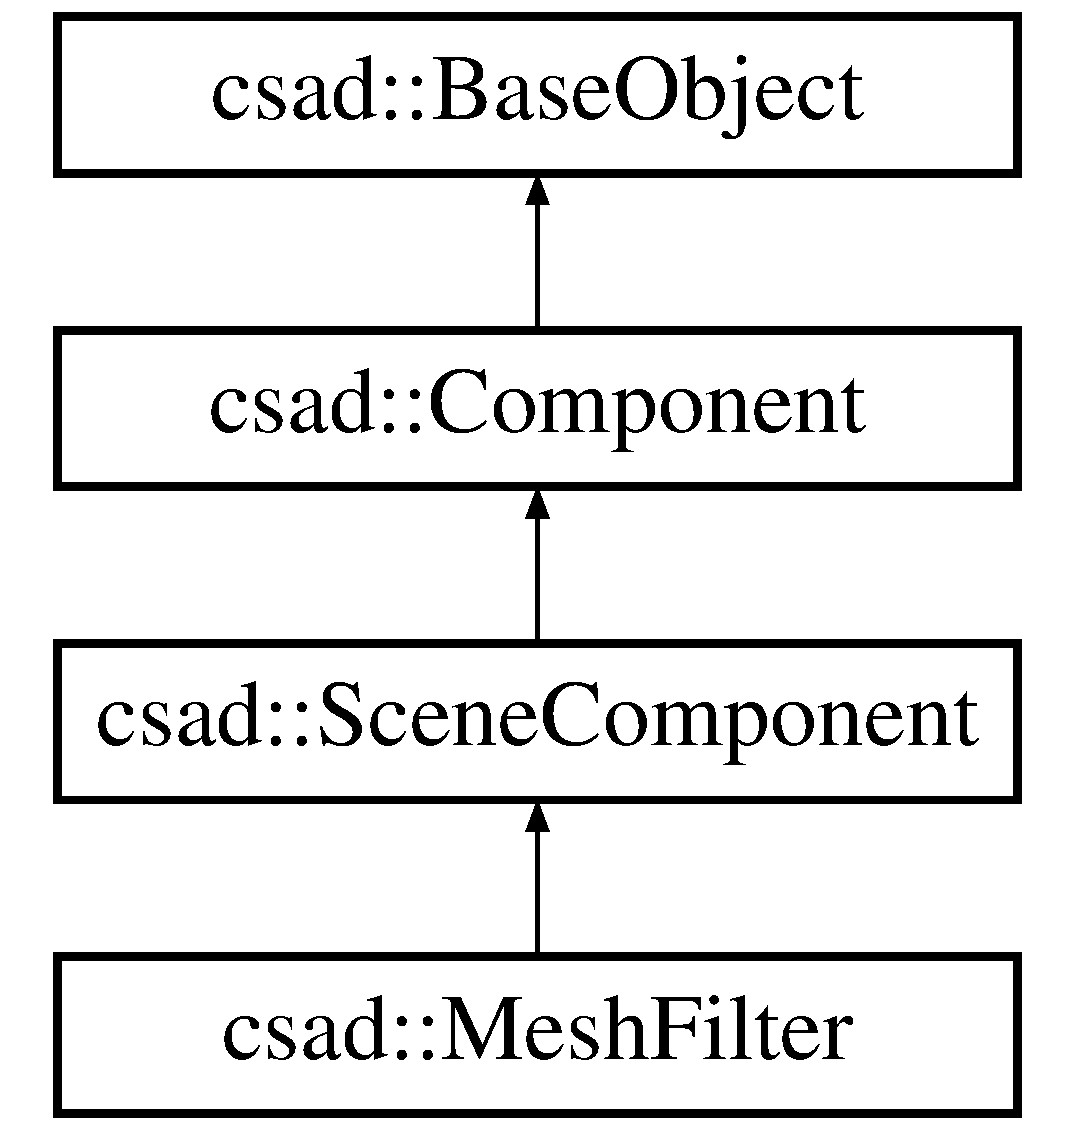
\includegraphics[height=4.000000cm]{classcsad_1_1_mesh_filter}
\end{center}
\end{figure}
\subsection*{Public Member Functions}
\begin{DoxyCompactItemize}
\item 
\hypertarget{classcsad_1_1_mesh_filter_ab2ab22b032aa9cfa7d67a26d61ae3a5c}{\-\_\-\-F\-O\-R\-C\-E\-I\-N\-L\-I\-N\-E \hyperlink{classcsad_1_1_lighting_model}{Lighting\-Model} $\ast$ \hyperlink{classcsad_1_1_mesh_filter_ab2ab22b032aa9cfa7d67a26d61ae3a5c}{get\-Lighting\-Model} ()}\label{classcsad_1_1_mesh_filter_ab2ab22b032aa9cfa7d67a26d61ae3a5c}

\begin{DoxyCompactList}\small\item\em Return used \hyperlink{classcsad_1_1_lighting_model}{Lighting\-Model}. \end{DoxyCompactList}\item 
\hypertarget{classcsad_1_1_mesh_filter_a6c416735a6272930e9d8534d17d444ee}{\-\_\-\-F\-O\-R\-C\-E\-I\-N\-L\-I\-N\-E \hyperlink{classcsad_1_1_material}{Material} $\ast$ \hyperlink{classcsad_1_1_mesh_filter_a6c416735a6272930e9d8534d17d444ee}{get\-Material} ()}\label{classcsad_1_1_mesh_filter_a6c416735a6272930e9d8534d17d444ee}

\begin{DoxyCompactList}\small\item\em Return used material. \end{DoxyCompactList}\item 
\hypertarget{classcsad_1_1_mesh_filter_a566d03045466a6d9b800de1764575b6f}{C\-S\-A\-D\-\_\-\-A\-P\-I \hyperlink{classcsad_1_1_mesh}{Mesh} $\ast$ \hyperlink{classcsad_1_1_mesh_filter_a566d03045466a6d9b800de1764575b6f}{get\-Mesh} ()}\label{classcsad_1_1_mesh_filter_a566d03045466a6d9b800de1764575b6f}

\begin{DoxyCompactList}\small\item\em Return view geometry. \end{DoxyCompactList}\item 
\hypertarget{classcsad_1_1_mesh_filter_a947c5f3197434a7c9e918958e5085912}{\-\_\-\-F\-O\-R\-C\-E\-I\-N\-L\-I\-N\-E \hyperlink{classcsad_1_1_shader}{Shader} $\ast$ \hyperlink{classcsad_1_1_mesh_filter_a947c5f3197434a7c9e918958e5085912}{get\-Shader} ()}\label{classcsad_1_1_mesh_filter_a947c5f3197434a7c9e918958e5085912}

\begin{DoxyCompactList}\small\item\em Return used shader. \end{DoxyCompactList}\item 
\hypertarget{classcsad_1_1_mesh_filter_a0bbe27e608bc97c12b3ad6ab2002f8d2}{C\-S\-A\-D\-\_\-\-A\-P\-I \hyperlink{classcsad_1_1_v_b_o_mesh}{V\-B\-O\-Mesh} $\ast$ \hyperlink{classcsad_1_1_mesh_filter_a0bbe27e608bc97c12b3ad6ab2002f8d2}{get\-V\-B\-O\-Mesh} ()}\label{classcsad_1_1_mesh_filter_a0bbe27e608bc97c12b3ad6ab2002f8d2}

\begin{DoxyCompactList}\small\item\em Return vbo view geometry. \end{DoxyCompactList}\item 
\hypertarget{classcsad_1_1_mesh_filter_a6f02c76e82a5228fa57036094cb31421}{C\-S\-A\-D\-\_\-\-A\-P\-I void $\ast$ \hyperlink{classcsad_1_1_mesh_filter_a6f02c76e82a5228fa57036094cb31421}{set} (unsigned \-\_\-int32, void $\ast$)}\label{classcsad_1_1_mesh_filter_a6f02c76e82a5228fa57036094cb31421}

\begin{DoxyCompactList}\small\item\em used for any interface commands. \end{DoxyCompactList}\item 
\hypertarget{classcsad_1_1_mesh_filter_a6fc1f22d3c8519043a0178fc68c3b80f}{C\-S\-A\-D\-\_\-\-A\-P\-I \hyperlink{classcsad_1_1_mesh_filter}{Mesh\-Filter} \& \hyperlink{classcsad_1_1_mesh_filter_a6fc1f22d3c8519043a0178fc68c3b80f}{set\-Lighting\-Model} (char $\ast$)}\label{classcsad_1_1_mesh_filter_a6fc1f22d3c8519043a0178fc68c3b80f}

\begin{DoxyCompactList}\small\item\em Set \hyperlink{classcsad_1_1_lighting_model}{Lighting\-Model} for use. \end{DoxyCompactList}\item 
\hypertarget{classcsad_1_1_mesh_filter_a10d68452775cc7c17e4d06b715ff5aad}{\-\_\-\-F\-O\-R\-C\-E\-I\-N\-L\-I\-N\-E \hyperlink{classcsad_1_1_mesh_filter}{Mesh\-Filter} \& \hyperlink{classcsad_1_1_mesh_filter_a10d68452775cc7c17e4d06b715ff5aad}{set\-Lighting\-Model} (const char $\ast$name)}\label{classcsad_1_1_mesh_filter_a10d68452775cc7c17e4d06b715ff5aad}

\begin{DoxyCompactList}\small\item\em Set \hyperlink{classcsad_1_1_lighting_model}{Lighting\-Model} for use. \end{DoxyCompactList}\item 
\hypertarget{classcsad_1_1_mesh_filter_a4fe8d1767431b43cee19c32535c1d294}{C\-S\-A\-D\-\_\-\-A\-P\-I \hyperlink{classcsad_1_1_mesh_filter}{Mesh\-Filter} \& \hyperlink{classcsad_1_1_mesh_filter_a4fe8d1767431b43cee19c32535c1d294}{set\-Lighting\-Model} (\hyperlink{classcsad_1_1_lighting_model}{Lighting\-Model} $\ast$)}\label{classcsad_1_1_mesh_filter_a4fe8d1767431b43cee19c32535c1d294}

\begin{DoxyCompactList}\small\item\em Set \hyperlink{classcsad_1_1_lighting_model}{Lighting\-Model} for use. \end{DoxyCompactList}\item 
\hypertarget{classcsad_1_1_mesh_filter_a2f943cf999049ec61cf5bdb6ba73aec8}{C\-S\-A\-D\-\_\-\-A\-P\-I \hyperlink{classcsad_1_1_mesh_filter}{Mesh\-Filter} \& \hyperlink{classcsad_1_1_mesh_filter_a2f943cf999049ec61cf5bdb6ba73aec8}{set\-Material} (char $\ast$)}\label{classcsad_1_1_mesh_filter_a2f943cf999049ec61cf5bdb6ba73aec8}

\begin{DoxyCompactList}\small\item\em Set material for use. \end{DoxyCompactList}\item 
\hypertarget{classcsad_1_1_mesh_filter_a0d57d5b460bde103167907662e651153}{\-\_\-\-F\-O\-R\-C\-E\-I\-N\-L\-I\-N\-E \hyperlink{classcsad_1_1_mesh_filter}{Mesh\-Filter} \& \hyperlink{classcsad_1_1_mesh_filter_a0d57d5b460bde103167907662e651153}{set\-Material} (const char $\ast$name)}\label{classcsad_1_1_mesh_filter_a0d57d5b460bde103167907662e651153}

\begin{DoxyCompactList}\small\item\em Set material for use. \end{DoxyCompactList}\item 
\hypertarget{classcsad_1_1_mesh_filter_ab77f373f91f775a46160aa9d03bf56a5}{C\-S\-A\-D\-\_\-\-A\-P\-I \hyperlink{classcsad_1_1_mesh_filter}{Mesh\-Filter} \& \hyperlink{classcsad_1_1_mesh_filter_ab77f373f91f775a46160aa9d03bf56a5}{set\-Material} (\hyperlink{classcsad_1_1_material}{Material} $\ast$)}\label{classcsad_1_1_mesh_filter_ab77f373f91f775a46160aa9d03bf56a5}

\begin{DoxyCompactList}\small\item\em Set material for use. \end{DoxyCompactList}\item 
\hypertarget{classcsad_1_1_mesh_filter_aba4e761c4a223bf1f01d92e4106bdeb7}{C\-S\-A\-D\-\_\-\-A\-P\-I \hyperlink{classcsad_1_1_mesh_filter}{Mesh\-Filter} \& \hyperlink{classcsad_1_1_mesh_filter_aba4e761c4a223bf1f01d92e4106bdeb7}{set\-Mesh} (char $\ast$)}\label{classcsad_1_1_mesh_filter_aba4e761c4a223bf1f01d92e4106bdeb7}

\begin{DoxyCompactList}\small\item\em Specifies the visible geometry by name. \end{DoxyCompactList}\item 
\hypertarget{classcsad_1_1_mesh_filter_ae31e1bfe9ee6227689acb6d20f241505}{\-\_\-\-F\-O\-R\-C\-E\-I\-N\-L\-I\-N\-E \hyperlink{classcsad_1_1_mesh_filter}{Mesh\-Filter} \& \hyperlink{classcsad_1_1_mesh_filter_ae31e1bfe9ee6227689acb6d20f241505}{set\-Mesh} (const char $\ast$name)}\label{classcsad_1_1_mesh_filter_ae31e1bfe9ee6227689acb6d20f241505}

\begin{DoxyCompactList}\small\item\em Set view geometry. \end{DoxyCompactList}\item 
\hypertarget{classcsad_1_1_mesh_filter_ac930a7e52f86a271f711efe943c1471b}{C\-S\-A\-D\-\_\-\-A\-P\-I \hyperlink{classcsad_1_1_mesh_filter}{Mesh\-Filter} \& \hyperlink{classcsad_1_1_mesh_filter_ac930a7e52f86a271f711efe943c1471b}{set\-Mesh} (\hyperlink{classcsad_1_1_base_mesh}{Base\-Mesh} $\ast$)}\label{classcsad_1_1_mesh_filter_ac930a7e52f86a271f711efe943c1471b}

\begin{DoxyCompactList}\small\item\em Specifies the visible geometry. \end{DoxyCompactList}\item 
\hypertarget{classcsad_1_1_mesh_filter_a0b7827a2ea54e3d36b219d4f978c917c}{C\-S\-A\-D\-\_\-\-A\-P\-I \hyperlink{classcsad_1_1_mesh_filter}{Mesh\-Filter} \& \hyperlink{classcsad_1_1_mesh_filter_a0b7827a2ea54e3d36b219d4f978c917c}{set\-Shader} (char $\ast$)}\label{classcsad_1_1_mesh_filter_a0b7827a2ea54e3d36b219d4f978c917c}

\begin{DoxyCompactList}\small\item\em Set shader for use. \end{DoxyCompactList}\item 
\hypertarget{classcsad_1_1_mesh_filter_af961ebe8b8bb7d13538f6e6b3f8e9608}{\-\_\-\-F\-O\-R\-C\-E\-I\-N\-L\-I\-N\-E \hyperlink{classcsad_1_1_mesh_filter}{Mesh\-Filter} \& \hyperlink{classcsad_1_1_mesh_filter_af961ebe8b8bb7d13538f6e6b3f8e9608}{set\-Shader} (const char $\ast$name)}\label{classcsad_1_1_mesh_filter_af961ebe8b8bb7d13538f6e6b3f8e9608}

\begin{DoxyCompactList}\small\item\em Set shader for use. \end{DoxyCompactList}\item 
\hypertarget{classcsad_1_1_mesh_filter_a67a062e40e51c5f5528fff391d011c0b}{C\-S\-A\-D\-\_\-\-A\-P\-I \hyperlink{classcsad_1_1_mesh_filter}{Mesh\-Filter} \& \hyperlink{classcsad_1_1_mesh_filter_a67a062e40e51c5f5528fff391d011c0b}{set\-Shader} (\hyperlink{classcsad_1_1_shader}{Shader} $\ast$)}\label{classcsad_1_1_mesh_filter_a67a062e40e51c5f5528fff391d011c0b}

\begin{DoxyCompactList}\small\item\em Set shader for use. \end{DoxyCompactList}\end{DoxyCompactItemize}
\subsection*{Additional Inherited Members}


\subsection{Detailed Description}
\hyperlink{classcsad_1_1_mesh_filter}{Mesh\-Filter} -\/ a component of a graphical object. 

The mediator unifying component properties and models of geometry, allowing you to link the object's position with his image, performs the functions of a Manager of a geometry for a given object in the scene.

\begin{DoxyVerb}  csad::Graph::graph().getScene("MyScene")->getRoot()->addComponent<MeshFilter>()->setMesh( csad::Mesh::Quad() );
\end{DoxyVerb}


\begin{DoxySeeAlso}{See Also}
\hyperlink{group__scene}{csad\-: scene} \hyperlink{classcsad_1_1_mesh}{Mesh} \hyperlink{classcsad_1_1_material}{Material} \hyperlink{classcsad_1_1_shader}{Shader} \hyperlink{classcsad_1_1_scene_component}{Scene\-Component} \hyperlink{classcsad_1_1_transform}{Transform} 
\end{DoxySeeAlso}

\hypertarget{classcsad_1_1_module}{\section{csad\-:\-:Module Class Reference}
\label{classcsad_1_1_module}\index{csad\-::\-Module@{csad\-::\-Module}}
}


\hyperlink{classcsad_1_1_module}{Module} -\/ dynamic module contains system components.  


Inheritance diagram for csad\-:\-:Module\-:\begin{figure}[H]
\begin{center}
\leavevmode
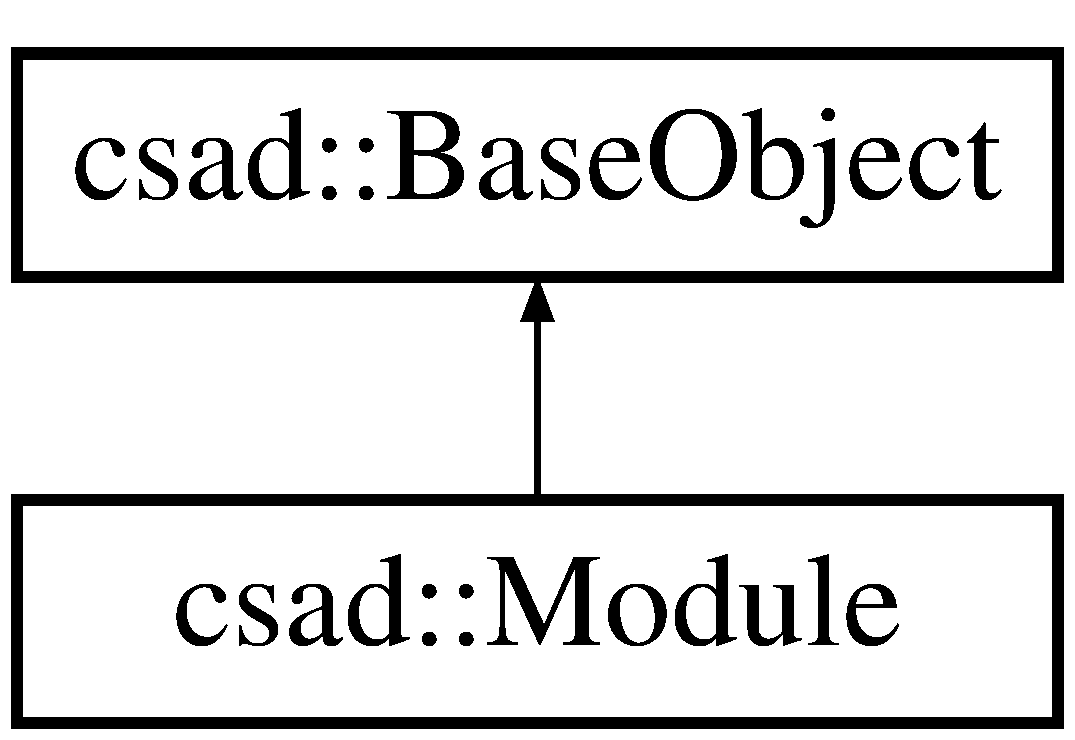
\includegraphics[height=2.000000cm]{classcsad_1_1_module}
\end{center}
\end{figure}
\subsection*{Public Member Functions}
\begin{DoxyCompactItemize}
\item 
\hypertarget{classcsad_1_1_module_acec7f78a1e05c61c6670e77684a9949d}{\-\_\-\-F\-O\-R\-C\-E\-I\-N\-L\-I\-N\-E void $\ast$ \hyperlink{classcsad_1_1_module_acec7f78a1e05c61c6670e77684a9949d}{get\-Proc} (char $\ast$name)}\label{classcsad_1_1_module_acec7f78a1e05c61c6670e77684a9949d}

\begin{DoxyCompactList}\small\item\em returns the method by name \end{DoxyCompactList}\item 
\hypertarget{classcsad_1_1_module_ab36b4578493a32edd48eb3007540ef47}{\-\_\-\-F\-O\-R\-C\-E\-I\-N\-L\-I\-N\-E bool \hyperlink{classcsad_1_1_module_ab36b4578493a32edd48eb3007540ef47}{is\-Init} ()}\label{classcsad_1_1_module_ab36b4578493a32edd48eb3007540ef47}

\begin{DoxyCompactList}\small\item\em returns true if the module is active \end{DoxyCompactList}\item 
\hypertarget{classcsad_1_1_module_af65981fd5d57f26c0afe612ead88bb21}{C\-S\-A\-D\-\_\-\-A\-P\-I void $\ast$ \hyperlink{classcsad_1_1_module_af65981fd5d57f26c0afe612ead88bb21}{set} (unsigned \-\_\-int32, void $\ast$)}\label{classcsad_1_1_module_af65981fd5d57f26c0afe612ead88bb21}

\begin{DoxyCompactList}\small\item\em used for any interface commands. \end{DoxyCompactList}\end{DoxyCompactItemize}
\subsection*{Additional Inherited Members}


\subsection{Detailed Description}
\hyperlink{classcsad_1_1_module}{Module} -\/ dynamic module contains system components. 

Allows you to connect additional components in the form of libraries, extending the basic features.

\begin{DoxyVerb}* <Module path="/mycomponents/app.so.1" />
* <Module path="/mycomponents/app.dll" />
*
* <Module path="/mycomponents/" lib="app" />
* \end{DoxyVerb}


\begin{DoxySeeAlso}{See Also}
\hyperlink{group__core}{csad\-: core} 
\end{DoxySeeAlso}

\hypertarget{classcsad_1_1_mouse}{\section{csad\-:\-:Mouse Class Reference}
\label{classcsad_1_1_mouse}\index{csad\-::\-Mouse@{csad\-::\-Mouse}}
}


\hyperlink{classcsad_1_1_mouse}{Mouse} -\/ the object input system, platform dependent.  




Inherits csad\-::\-Base\-Mouse.

\subsection*{Public Member Functions}
\begin{DoxyCompactItemize}
\item 
\hypertarget{classcsad_1_1_mouse_aff936deb785be6c3790e2fc187d88109}{P\-L\-A\-T\-F\-O\-R\-M\-\_\-\-A\-P\-I void $\ast$ \hyperlink{classcsad_1_1_mouse_aff936deb785be6c3790e2fc187d88109}{set} (unsigned \-\_\-int32, void $\ast$)}\label{classcsad_1_1_mouse_aff936deb785be6c3790e2fc187d88109}

\begin{DoxyCompactList}\small\item\em used for any interface commands. \end{DoxyCompactList}\end{DoxyCompactItemize}
\subsection*{Additional Inherited Members}


\subsection{Detailed Description}
\hyperlink{classcsad_1_1_mouse}{Mouse} -\/ the object input system, platform dependent. 

For description in the configuration\-: \begin{DoxyVerb}  <Mouse name="имя в системе" driver="параметры драйвера" />
\end{DoxyVerb}
 \begin{DoxySeeAlso}{See Also}
\hyperlink{group__input}{csad\-: input} 
\end{DoxySeeAlso}

\hypertarget{classcsad_1_1_net_connection}{\section{csad\-:\-:Net\-Connection Class Reference}
\label{classcsad_1_1_net_connection}\index{csad\-::\-Net\-Connection@{csad\-::\-Net\-Connection}}
}


\hyperlink{classcsad_1_1_net_connection}{Net\-Connection} -\/ network connection.  


\subsection*{Public Types}
\begin{DoxyCompactItemize}
\item 
enum \hyperlink{classcsad_1_1_net_connection_a3b8242f34d97fe051d6eab451b6db3b5}{Mode} \{ \hyperlink{classcsad_1_1_net_connection_a3b8242f34d97fe051d6eab451b6db3b5a47d79c745230e16a4402daabece4788b}{N\-C\-\_\-\-T\-C\-P}, 
\hyperlink{classcsad_1_1_net_connection_a3b8242f34d97fe051d6eab451b6db3b5a9bc0746a60d6a49de4c09e67586ad7d9}{N\-C\-\_\-\-U\-D\-P}, 
\hyperlink{classcsad_1_1_net_connection_a3b8242f34d97fe051d6eab451b6db3b5a67c9b49521cbc221e928764cf96dbf4d}{N\-C\-\_\-\-R\-A\-W}
 \}
\begin{DoxyCompactList}\small\item\em socket mode \end{DoxyCompactList}\end{DoxyCompactItemize}
\subsection*{Public Member Functions}
\begin{DoxyCompactItemize}
\item 
\hypertarget{classcsad_1_1_net_connection_a5072b9dd2d289ce7b3654f0988fa1d21}{\-\_\-\-F\-O\-R\-C\-E\-I\-N\-L\-I\-N\-E \hyperlink{classcsad_1_1_net_connection_a5072b9dd2d289ce7b3654f0988fa1d21}{Net\-Connection} (char $\ast$)}\label{classcsad_1_1_net_connection_a5072b9dd2d289ce7b3654f0988fa1d21}

\begin{DoxyCompactList}\small\item\em create connection \end{DoxyCompactList}\item 
\hypertarget{classcsad_1_1_net_connection_af5eb90166c8ba105b07159d6337a85e7}{\-\_\-\-F\-O\-R\-C\-E\-I\-N\-L\-I\-N\-E \hyperlink{classcsad_1_1_net_connection}{Net\-Connection} $\ast$ \hyperlink{classcsad_1_1_net_connection_af5eb90166c8ba105b07159d6337a85e7}{accept} (char $\ast$)}\label{classcsad_1_1_net_connection_af5eb90166c8ba105b07159d6337a85e7}

\begin{DoxyCompactList}\small\item\em recive connection and create new \hyperlink{classcsad_1_1_net_connection}{Net\-Connection}. \end{DoxyCompactList}\item 
\hypertarget{classcsad_1_1_net_connection_ab728f123450001d146cfd3599a0712d7}{\-\_\-\-F\-O\-R\-C\-E\-I\-N\-L\-I\-N\-E unsigned \-\_\-int32 \hyperlink{classcsad_1_1_net_connection_ab728f123450001d146cfd3599a0712d7}{addr} ()}\label{classcsad_1_1_net_connection_ab728f123450001d146cfd3599a0712d7}

\begin{DoxyCompactList}\small\item\em return connection or last recv data addres. \end{DoxyCompactList}\item 
\hypertarget{classcsad_1_1_net_connection_a6b9a1925025010ab14a739311174bb1f}{\-\_\-\-F\-O\-R\-C\-E\-I\-N\-L\-I\-N\-E bool \hyperlink{classcsad_1_1_net_connection_a6b9a1925025010ab14a739311174bb1f}{close} ()}\label{classcsad_1_1_net_connection_a6b9a1925025010ab14a739311174bb1f}

\begin{DoxyCompactList}\small\item\em Close socket. \end{DoxyCompactList}\item 
\hypertarget{classcsad_1_1_net_connection_ac1c3c64ca6d4811931a5fc430657d8f7}{\-\_\-\-F\-O\-R\-C\-E\-I\-N\-L\-I\-N\-E bool \hyperlink{classcsad_1_1_net_connection_ac1c3c64ca6d4811931a5fc430657d8f7}{connect} ()}\label{classcsad_1_1_net_connection_ac1c3c64ca6d4811931a5fc430657d8f7}

\begin{DoxyCompactList}\small\item\em Connect. \end{DoxyCompactList}\item 
\hypertarget{classcsad_1_1_net_connection_a66b082952ef88366496a30331f13c3a9}{\-\_\-\-F\-O\-R\-C\-E\-I\-N\-L\-I\-N\-E bool \hyperlink{classcsad_1_1_net_connection_a66b082952ef88366496a30331f13c3a9}{open} ()}\label{classcsad_1_1_net_connection_a66b082952ef88366496a30331f13c3a9}

\begin{DoxyCompactList}\small\item\em Open socket. \end{DoxyCompactList}\item 
\hypertarget{classcsad_1_1_net_connection_acb26734ada988518925467b18447d54e}{\-\_\-\-F\-O\-R\-C\-E\-I\-N\-L\-I\-N\-E \-\_\-int32 \hyperlink{classcsad_1_1_net_connection_acb26734ada988518925467b18447d54e}{port} ()}\label{classcsad_1_1_net_connection_acb26734ada988518925467b18447d54e}

\begin{DoxyCompactList}\small\item\em return connection port. \end{DoxyCompactList}\item 
\hypertarget{classcsad_1_1_net_connection_aff8bdebec5c06a7667f196d25584ba9e}{\-\_\-\-F\-O\-R\-C\-E\-I\-N\-L\-I\-N\-E int \hyperlink{classcsad_1_1_net_connection_aff8bdebec5c06a7667f196d25584ba9e}{read} (void $\ast$data, unsigned int size)}\label{classcsad_1_1_net_connection_aff8bdebec5c06a7667f196d25584ba9e}

\begin{DoxyCompactList}\small\item\em recive data \end{DoxyCompactList}\item 
\hypertarget{classcsad_1_1_net_connection_a29b59fc5dd401fff7f4cc5e898ba1bef}{\-\_\-\-F\-O\-R\-C\-E\-I\-N\-L\-I\-N\-E void \hyperlink{classcsad_1_1_net_connection_a29b59fc5dd401fff7f4cc5e898ba1bef}{set\-Addr} (char a, char b, char c, char d)}\label{classcsad_1_1_net_connection_a29b59fc5dd401fff7f4cc5e898ba1bef}

\begin{DoxyCompactList}\small\item\em set connection addres. \end{DoxyCompactList}\item 
\hypertarget{classcsad_1_1_net_connection_a1c1000c61de1d3e97400eebbe7290726}{\-\_\-\-F\-O\-R\-C\-E\-I\-N\-L\-I\-N\-E void \hyperlink{classcsad_1_1_net_connection_a1c1000c61de1d3e97400eebbe7290726}{set\-Mode} (unsigned int mode)}\label{classcsad_1_1_net_connection_a1c1000c61de1d3e97400eebbe7290726}

\begin{DoxyCompactList}\small\item\em set connection mode \end{DoxyCompactList}\item 
\hypertarget{classcsad_1_1_net_connection_ac888de6d8682f77b9397baf4678064dd}{\-\_\-\-F\-O\-R\-C\-E\-I\-N\-L\-I\-N\-E void \hyperlink{classcsad_1_1_net_connection_ac888de6d8682f77b9397baf4678064dd}{set\-Port} (\-\_\-int32 \hyperlink{classcsad_1_1_net_connection_acb26734ada988518925467b18447d54e}{port})}\label{classcsad_1_1_net_connection_ac888de6d8682f77b9397baf4678064dd}

\begin{DoxyCompactList}\small\item\em set port connection, or for open listening \end{DoxyCompactList}\item 
\hypertarget{classcsad_1_1_net_connection_a62442d45c39493be16ce3d5377aede73}{\-\_\-\-F\-O\-R\-C\-E\-I\-N\-L\-I\-N\-E int \hyperlink{classcsad_1_1_net_connection_a62442d45c39493be16ce3d5377aede73}{write} (void $\ast$data, unsigned int size)}\label{classcsad_1_1_net_connection_a62442d45c39493be16ce3d5377aede73}

\begin{DoxyCompactList}\small\item\em send data \end{DoxyCompactList}\end{DoxyCompactItemize}


\subsection{Detailed Description}
\hyperlink{classcsad_1_1_net_connection}{Net\-Connection} -\/ network connection. 

For example U\-D\-P\-: \begin{DoxyVerb}  NetConnection connection;
  connection.setMode(NC_UDP);
  connection.setPort(2000);
  connection.setAddr(0,0,0,0);
  connection.open();
  char data[256];
  connection.write(data,256);
  while (connection.read(data,256)==0);
  unsigned _int32 recvAddr=connection.addr();
  connection.setAddr(192,168,102,10);
  while (connection.write(data,256)==0);
  connection.close();
\end{DoxyVerb}


For example T\-C\-P client\-: \begin{DoxyVerb}  NetConnection connection;
  connection.setMode(NC_TCP);
  connection.setPort(2000);
  connection.setAddr(192,168,102,20);
  connection.connect();
  char data[256];
  connection.write(data,256);
  connection.close();
\end{DoxyVerb}


\begin{DoxySeeAlso}{See Also}
\hyperlink{group__platform}{csad\-: platform} 
\end{DoxySeeAlso}


\subsection{Member Enumeration Documentation}
\hypertarget{classcsad_1_1_net_connection_a3b8242f34d97fe051d6eab451b6db3b5}{\index{csad\-::\-Net\-Connection@{csad\-::\-Net\-Connection}!Mode@{Mode}}
\index{Mode@{Mode}!csad::NetConnection@{csad\-::\-Net\-Connection}}
\subsubsection[{Mode}]{\setlength{\rightskip}{0pt plus 5cm}enum {\bf csad\-::\-Net\-Connection\-::\-Mode}}}\label{classcsad_1_1_net_connection_a3b8242f34d97fe051d6eab451b6db3b5}


socket mode 

\begin{Desc}
\item[Enumerator]\par
\begin{description}
\index{N\-C\-\_\-\-T\-C\-P@{N\-C\-\_\-\-T\-C\-P}!csad\-::\-Net\-Connection@{csad\-::\-Net\-Connection}}\index{csad\-::\-Net\-Connection@{csad\-::\-Net\-Connection}!N\-C\-\_\-\-T\-C\-P@{N\-C\-\_\-\-T\-C\-P}}\item[{\em 
\hypertarget{classcsad_1_1_net_connection_a3b8242f34d97fe051d6eab451b6db3b5a47d79c745230e16a4402daabece4788b}{N\-C\-\_\-\-T\-C\-P}\label{classcsad_1_1_net_connection_a3b8242f34d97fe051d6eab451b6db3b5a47d79c745230e16a4402daabece4788b}
}]create T\-C\-P connection \index{N\-C\-\_\-\-U\-D\-P@{N\-C\-\_\-\-U\-D\-P}!csad\-::\-Net\-Connection@{csad\-::\-Net\-Connection}}\index{csad\-::\-Net\-Connection@{csad\-::\-Net\-Connection}!N\-C\-\_\-\-U\-D\-P@{N\-C\-\_\-\-U\-D\-P}}\item[{\em 
\hypertarget{classcsad_1_1_net_connection_a3b8242f34d97fe051d6eab451b6db3b5a9bc0746a60d6a49de4c09e67586ad7d9}{N\-C\-\_\-\-U\-D\-P}\label{classcsad_1_1_net_connection_a3b8242f34d97fe051d6eab451b6db3b5a9bc0746a60d6a49de4c09e67586ad7d9}
}]create U\-D\-P connection \index{N\-C\-\_\-\-R\-A\-W@{N\-C\-\_\-\-R\-A\-W}!csad\-::\-Net\-Connection@{csad\-::\-Net\-Connection}}\index{csad\-::\-Net\-Connection@{csad\-::\-Net\-Connection}!N\-C\-\_\-\-R\-A\-W@{N\-C\-\_\-\-R\-A\-W}}\item[{\em 
\hypertarget{classcsad_1_1_net_connection_a3b8242f34d97fe051d6eab451b6db3b5a67c9b49521cbc221e928764cf96dbf4d}{N\-C\-\_\-\-R\-A\-W}\label{classcsad_1_1_net_connection_a3b8242f34d97fe051d6eab451b6db3b5a67c9b49521cbc221e928764cf96dbf4d}
}]create R\-A\-W connection \end{description}
\end{Desc}

\hypertarget{classcsad_1_1_node_x_m_l}{\section{csad\-:\-:Node\-X\-M\-L Class Reference}
\label{classcsad_1_1_node_x_m_l}\index{csad\-::\-Node\-X\-M\-L@{csad\-::\-Node\-X\-M\-L}}
}


\hyperlink{classcsad_1_1_node_x_m_l}{Node\-X\-M\-L} -\/ элемент данных xml файла.  


\subsection*{Public Member Functions}
\begin{DoxyCompactItemize}
\item 
\hypertarget{classcsad_1_1_node_x_m_l_ac0651771bc96fba9d355a35d095adacd}{\-\_\-\-F\-O\-R\-C\-E\-I\-N\-L\-I\-N\-E const char $\ast$ \hyperlink{classcsad_1_1_node_x_m_l_ac0651771bc96fba9d355a35d095adacd}{get\-Char\-Name} ()}\label{classcsad_1_1_node_x_m_l_ac0651771bc96fba9d355a35d095adacd}

\begin{DoxyCompactList}\small\item\em Returns the tag name. \end{DoxyCompactList}\item 
C\-S\-A\-D\-\_\-\-A\-P\-I \hyperlink{classcsad_1_1_node_x_m_l}{Node\-X\-M\-L} $\ast$ \hyperlink{classcsad_1_1_node_x_m_l_a9c768e31866e7f8439485baaf24d7599}{get\-Child} (char $\ast$name)
\item 
\hypertarget{classcsad_1_1_node_x_m_l_a6d610edfac400cb78e0e94743dd3da1a}{\-\_\-\-F\-O\-R\-C\-E\-I\-N\-L\-I\-N\-E \hyperlink{classbt_1_1_short_string}{Short\-String} \& \hyperlink{classcsad_1_1_node_x_m_l_a6d610edfac400cb78e0e94743dd3da1a}{get\-Name} ()}\label{classcsad_1_1_node_x_m_l_a6d610edfac400cb78e0e94743dd3da1a}

\begin{DoxyCompactList}\small\item\em Returns the tag name. \end{DoxyCompactList}\item 
\hypertarget{classcsad_1_1_node_x_m_l_a60de99ca441f3dbb28a998ad0a8ce984}{\-\_\-\-F\-O\-R\-C\-E\-I\-N\-L\-I\-N\-E \hyperlink{classbt_1_1_void_vector}{Node\-X\-M\-L\-List} \& \hyperlink{classcsad_1_1_node_x_m_l_a60de99ca441f3dbb28a998ad0a8ce984}{get\-Node\-List} ()}\label{classcsad_1_1_node_x_m_l_a60de99ca441f3dbb28a998ad0a8ce984}

\begin{DoxyCompactList}\small\item\em возвращает список дочерних элементов \end{DoxyCompactList}\item 
\hypertarget{classcsad_1_1_node_x_m_l_a6f445711ee951f55e6a675167b8826b4}{\-\_\-\-F\-O\-R\-C\-E\-I\-N\-L\-I\-N\-E \hyperlink{classbt_1_1_parameters_list}{Parameters\-List} \& \hyperlink{classcsad_1_1_node_x_m_l_a6f445711ee951f55e6a675167b8826b4}{get\-Parameter\-List} ()}\label{classcsad_1_1_node_x_m_l_a6f445711ee951f55e6a675167b8826b4}

\begin{DoxyCompactList}\small\item\em взвращает список параметров тега \end{DoxyCompactList}\item 
\hypertarget{classcsad_1_1_node_x_m_l_a5081573b0ee193c4378399171258bf66}{C\-S\-A\-D\-\_\-\-A\-P\-I void \hyperlink{classcsad_1_1_node_x_m_l_a5081573b0ee193c4378399171258bf66}{set\-Name} (char $\ast$name)}\label{classcsad_1_1_node_x_m_l_a5081573b0ee193c4378399171258bf66}

\begin{DoxyCompactList}\small\item\em Sets the tag name. \end{DoxyCompactList}\item 
\hypertarget{classcsad_1_1_node_x_m_l_a59d3af4891f5a5a329c0e220e3926a1b}{\-\_\-\-F\-O\-R\-C\-E\-I\-N\-L\-I\-N\-E void \hyperlink{classcsad_1_1_node_x_m_l_a59d3af4891f5a5a329c0e220e3926a1b}{set\-Name} (const char $\ast$name)}\label{classcsad_1_1_node_x_m_l_a59d3af4891f5a5a329c0e220e3926a1b}

\begin{DoxyCompactList}\small\item\em Sets the tag name. \end{DoxyCompactList}\item 
\hypertarget{classcsad_1_1_node_x_m_l_ab8ce317238560771c7adbce5c0fc7e95}{C\-S\-A\-D\-\_\-\-A\-P\-I void \hyperlink{classcsad_1_1_node_x_m_l_ab8ce317238560771c7adbce5c0fc7e95}{set\-Parent} (\hyperlink{classcsad_1_1_node_x_m_l}{Node\-X\-M\-L} $\ast$parent)}\label{classcsad_1_1_node_x_m_l_ab8ce317238560771c7adbce5c0fc7e95}

\begin{DoxyCompactList}\small\item\em устанавливает родительский элемент \end{DoxyCompactList}\end{DoxyCompactItemize}


\subsection{Detailed Description}
\hyperlink{classcsad_1_1_node_x_m_l}{Node\-X\-M\-L} -\/ элемент данных xml файла. 

\begin{DoxySeeAlso}{See Also}
\hyperlink{classcsad_1_1_format_x_m_l}{Format\-X\-M\-L}, \hyperlink{group__format}{csad\-: format} 
\end{DoxySeeAlso}


\subsection{Member Function Documentation}
\hypertarget{classcsad_1_1_node_x_m_l_a9c768e31866e7f8439485baaf24d7599}{\index{csad\-::\-Node\-X\-M\-L@{csad\-::\-Node\-X\-M\-L}!get\-Child@{get\-Child}}
\index{get\-Child@{get\-Child}!csad::NodeXML@{csad\-::\-Node\-X\-M\-L}}
\subsubsection[{get\-Child}]{\setlength{\rightskip}{0pt plus 5cm}C\-S\-A\-D\-\_\-\-A\-P\-I {\bf Node\-X\-M\-L}$\ast$ csad\-::\-Node\-X\-M\-L\-::get\-Child (
\begin{DoxyParamCaption}
\item[{char $\ast$}]{name}
\end{DoxyParamCaption}
)}}\label{classcsad_1_1_node_x_m_l_a9c768e31866e7f8439485baaf24d7599}
возвращает зависимый нод 
\begin{DoxyParams}{Parameters}
{\em name} & -\/ имя ноды \char`\"{}node\-Name\mbox{[}3\mbox{]}\char`\"{} \\
\hline
\end{DoxyParams}

\hypertarget{classcsad_1_1_object_manager}{\section{csad\-:\-:Object\-Manager Class Reference}
\label{classcsad_1_1_object_manager}\index{csad\-::\-Object\-Manager@{csad\-::\-Object\-Manager}}
}


\hyperlink{classcsad_1_1_object_manager}{Object\-Manager} -\/ tool organize objects. Is intended for storage of objects or containers components.  


Inheritance diagram for csad\-:\-:Object\-Manager\-:\begin{figure}[H]
\begin{center}
\leavevmode
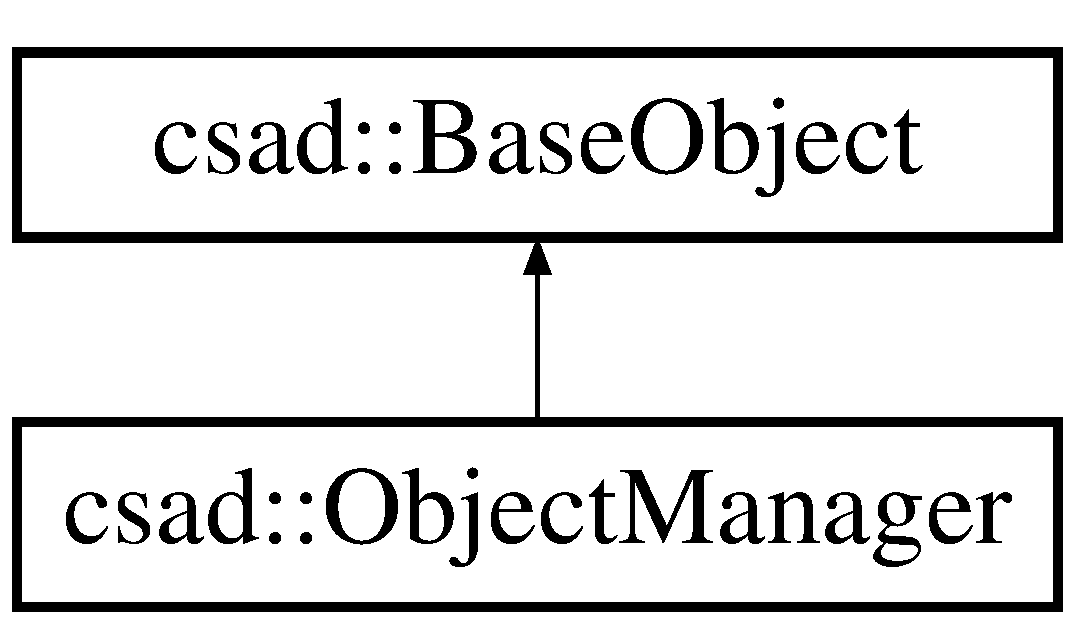
\includegraphics[height=2.000000cm]{classcsad_1_1_object_manager}
\end{center}
\end{figure}
\subsection*{Public Member Functions}
\begin{DoxyCompactItemize}
\item 
\hypertarget{classcsad_1_1_object_manager_ad68b9f728555715e9e6109e746c846d2}{C\-S\-A\-D\-\_\-\-A\-P\-I bool \hyperlink{classcsad_1_1_object_manager_ad68b9f728555715e9e6109e746c846d2}{add\-Object} (void $\ast$obj, char $\ast$name)}\label{classcsad_1_1_object_manager_ad68b9f728555715e9e6109e746c846d2}

\begin{DoxyCompactList}\small\item\em Adds the object and sets it a name. \end{DoxyCompactList}\item 
\hypertarget{classcsad_1_1_object_manager_a1d65df20a751e700f9185bf7eafe48dc}{\-\_\-\-F\-O\-R\-C\-E\-I\-N\-L\-I\-N\-E bool \hyperlink{classcsad_1_1_object_manager_a1d65df20a751e700f9185bf7eafe48dc}{add\-Object} (void $\ast$obj, const char $\ast$name=\char`\"{}\char`\"{})}\label{classcsad_1_1_object_manager_a1d65df20a751e700f9185bf7eafe48dc}

\begin{DoxyCompactList}\small\item\em Adds the object and sets it a name. \end{DoxyCompactList}\item 
\hypertarget{classcsad_1_1_object_manager_af712f3df6c4780a1a8a3971a65f49aeb}{C\-S\-A\-D\-\_\-\-A\-P\-I bool \hyperlink{classcsad_1_1_object_manager_af712f3df6c4780a1a8a3971a65f49aeb}{detach\-Object} (void $\ast$obj)}\label{classcsad_1_1_object_manager_af712f3df6c4780a1a8a3971a65f49aeb}

\begin{DoxyCompactList}\small\item\em Removes the object. \end{DoxyCompactList}\item 
\hypertarget{classcsad_1_1_object_manager_ad0e7a1030297c6516b8c963c5f65254e}{C\-S\-A\-D\-\_\-\-A\-P\-I const char $\ast$ \hyperlink{classcsad_1_1_object_manager_ad0e7a1030297c6516b8c963c5f65254e}{get\-Name} (void $\ast$obj)}\label{classcsad_1_1_object_manager_ad0e7a1030297c6516b8c963c5f65254e}

\begin{DoxyCompactList}\small\item\em Returns the name of the object if it is in the list. \end{DoxyCompactList}\item 
\hypertarget{classcsad_1_1_object_manager_a174709ddda723c6a7a71cf52c19292a6}{C\-S\-A\-D\-\_\-\-A\-P\-I void $\ast$ \hyperlink{classcsad_1_1_object_manager_a174709ddda723c6a7a71cf52c19292a6}{get\-Object} (char $\ast$name)}\label{classcsad_1_1_object_manager_a174709ddda723c6a7a71cf52c19292a6}

\begin{DoxyCompactList}\small\item\em Returns the object by name. \end{DoxyCompactList}\item 
\hypertarget{classcsad_1_1_object_manager_abab7b19acea4a580eb1b7e93de934e61}{C\-S\-A\-D\-\_\-\-A\-P\-I void $\ast$ \hyperlink{classcsad_1_1_object_manager_abab7b19acea4a580eb1b7e93de934e61}{get\-Object} (const char $\ast$name=\char`\"{}\char`\"{})}\label{classcsad_1_1_object_manager_abab7b19acea4a580eb1b7e93de934e61}

\begin{DoxyCompactList}\small\item\em Returns the object by name. \end{DoxyCompactList}\item 
\hypertarget{classcsad_1_1_object_manager_a582611819f43c8304394b1c6ec871241}{{\footnotesize template$<$typename T $>$ }\\\-\_\-\-F\-O\-R\-C\-E\-I\-N\-L\-I\-N\-E T $\ast$ \hyperlink{classcsad_1_1_object_manager_a582611819f43c8304394b1c6ec871241}{get\-Object} (char $\ast$name)}\label{classcsad_1_1_object_manager_a582611819f43c8304394b1c6ec871241}

\begin{DoxyCompactList}\small\item\em Returns the object by name, and leads to the specified type. \end{DoxyCompactList}\item 
\hypertarget{classcsad_1_1_object_manager_a248074aa1e25c0c64acc9b9bcd53b5bc}{{\footnotesize template$<$typename T $>$ }\\\-\_\-\-F\-O\-R\-C\-E\-I\-N\-L\-I\-N\-E T $\ast$ \hyperlink{classcsad_1_1_object_manager_a248074aa1e25c0c64acc9b9bcd53b5bc}{get\-Object} (const char $\ast$name=\char`\"{}\char`\"{})}\label{classcsad_1_1_object_manager_a248074aa1e25c0c64acc9b9bcd53b5bc}

\begin{DoxyCompactList}\small\item\em Returns the object by name, and leads to the specified type. \end{DoxyCompactList}\item 
\hypertarget{classcsad_1_1_object_manager_a1ecc9faccf025a2b55c189fad21f4d48}{\-\_\-\-F\-O\-R\-C\-E\-I\-N\-L\-I\-N\-E \hyperlink{classbt_1_1_map_name}{Objects\-List} \& \hyperlink{classcsad_1_1_object_manager_a1ecc9faccf025a2b55c189fad21f4d48}{get\-Objects} ()}\label{classcsad_1_1_object_manager_a1ecc9faccf025a2b55c189fad21f4d48}

\begin{DoxyCompactList}\small\item\em Returns a list of objects. \end{DoxyCompactList}\item 
\hypertarget{classcsad_1_1_object_manager_a69bf8143179b0ee6ae5554f212e64077}{C\-S\-A\-D\-\_\-\-A\-P\-I bool \hyperlink{classcsad_1_1_object_manager_a69bf8143179b0ee6ae5554f212e64077}{remove\-Object} (char $\ast$name)}\label{classcsad_1_1_object_manager_a69bf8143179b0ee6ae5554f212e64077}

\begin{DoxyCompactList}\small\item\em Removes the connection object named. \end{DoxyCompactList}\item 
\hypertarget{classcsad_1_1_object_manager_a1a5ae637929f9a0b75fe5744108fd1d1}{C\-S\-A\-D\-\_\-\-A\-P\-I bool \hyperlink{classcsad_1_1_object_manager_a1a5ae637929f9a0b75fe5744108fd1d1}{remove\-Object} (const char $\ast$name=\char`\"{}\char`\"{})}\label{classcsad_1_1_object_manager_a1a5ae637929f9a0b75fe5744108fd1d1}

\begin{DoxyCompactList}\small\item\em Removes the connection object named. \end{DoxyCompactList}\item 
\hypertarget{classcsad_1_1_object_manager_a16539e67e32f91a63432e89e30d4f30b}{C\-S\-A\-D\-\_\-\-A\-P\-I void $\ast$ \hyperlink{classcsad_1_1_object_manager_a16539e67e32f91a63432e89e30d4f30b}{set} (unsigned \-\_\-int32, void $\ast$)}\label{classcsad_1_1_object_manager_a16539e67e32f91a63432e89e30d4f30b}

\begin{DoxyCompactList}\small\item\em used for any interface commands. \end{DoxyCompactList}\end{DoxyCompactItemize}
\subsection*{Static Public Member Functions}
\begin{DoxyCompactItemize}
\item 
\hypertarget{classcsad_1_1_object_manager_aedaeff827696471cc324b42b5f63cedd}{static C\-S\-A\-D\-\_\-\-A\-P\-I \hyperlink{classcsad_1_1_object_manager}{Object\-Manager} \& \hyperlink{classcsad_1_1_object_manager_aedaeff827696471cc324b42b5f63cedd}{manager} ()}\label{classcsad_1_1_object_manager_aedaeff827696471cc324b42b5f63cedd}

\begin{DoxyCompactList}\small\item\em root Manager objects \end{DoxyCompactList}\end{DoxyCompactItemize}
\subsection*{Additional Inherited Members}


\subsection{Detailed Description}
\hyperlink{classcsad_1_1_object_manager}{Object\-Manager} -\/ tool organize objects. Is intended for storage of objects or containers components. 

\begin{DoxySeeAlso}{See Also}
\hyperlink{group__core}{csad\-: core} 
\end{DoxySeeAlso}

\hypertarget{classcsad_1_1_render}{\section{csad\-:\-:Render Class Reference}
\label{classcsad_1_1_render}\index{csad\-::\-Render@{csad\-::\-Render}}
}


\hyperlink{classcsad_1_1_render}{Render} -\/ the basic methods of drawing.  


\subsection*{Static Public Member Functions}
\begin{DoxyCompactItemize}
\item 
\hypertarget{classcsad_1_1_render_a3bf2c83bd00a588b77c5739e6cf6be94}{static void \-\_\-\-F\-A\-S\-T\-C\-A\-L\-L \hyperlink{classcsad_1_1_render_a3bf2c83bd00a588b77c5739e6cf6be94}{Info} ()}\label{classcsad_1_1_render_a3bf2c83bd00a588b77c5739e6cf6be94}

\begin{DoxyCompactList}\small\item\em установка массивов gen\-::gen\-::tglmodel. \end{DoxyCompactList}\end{DoxyCompactItemize}


\subsection{Detailed Description}
\hyperlink{classcsad_1_1_render}{Render} -\/ the basic methods of drawing. 

\begin{DoxySeeAlso}{See Also}
\hyperlink{group__scene}{csad\-: scene} 
\end{DoxySeeAlso}

\hypertarget{classcsad_1_1_renderer}{\section{csad\-:\-:Renderer Class Reference}
\label{classcsad_1_1_renderer}\index{csad\-::\-Renderer@{csad\-::\-Renderer}}
}


\hyperlink{classcsad_1_1_renderer}{Renderer} -\/ class imaging using the active camera selected scene.  


Inheritance diagram for csad\-:\-:Renderer\-:\begin{figure}[H]
\begin{center}
\leavevmode
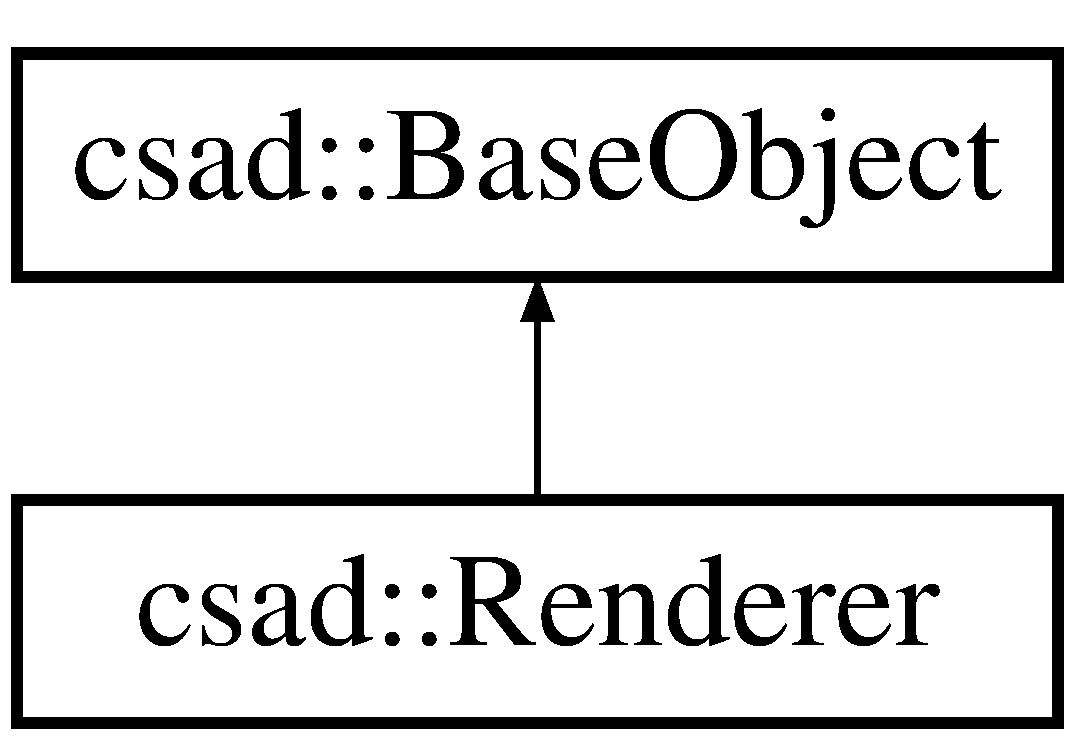
\includegraphics[height=2.000000cm]{classcsad_1_1_renderer}
\end{center}
\end{figure}
\subsection*{Public Types}
\begin{DoxyCompactItemize}
\item 
enum \hyperlink{classcsad_1_1_renderer_a112fd7f69525df52f65b47a62975538e}{M\-O\-D\-E\-S} \{ \\*
\hyperlink{classcsad_1_1_renderer_a112fd7f69525df52f65b47a62975538ead80d7d6b6aa720dc4bd7c630d93b976c}{N\-O\-S\-O\-R\-T} = 0x00000000, 
\hyperlink{classcsad_1_1_renderer_a112fd7f69525df52f65b47a62975538eaab6c6e6b28cdb5e5e5406d48ae44bade}{N\-O} = 0x00000000, 
\hyperlink{classcsad_1_1_renderer_a112fd7f69525df52f65b47a62975538ea2e4ee71bce65ed333a87b7abc851713c}{Z\-U\-P} = 0x00000001, 
\hyperlink{classcsad_1_1_renderer_a112fd7f69525df52f65b47a62975538eab78079ebc6178ac578d3f4fa65307d18}{Z\-D\-O\-W\-N} = 0x00000002, 
\\*
\hyperlink{classcsad_1_1_renderer_a112fd7f69525df52f65b47a62975538ead968921d8dd219f43c22fc612ef515b8}{T\-R\-E\-E} = 0x00000003
 \}
\end{DoxyCompactItemize}
\subsection*{Public Member Functions}
\begin{DoxyCompactItemize}
\item 
\hypertarget{classcsad_1_1_renderer_acd653a15f123687e861eecd85cf108e5}{\-\_\-\-F\-O\-R\-C\-E\-I\-N\-L\-I\-N\-E bool \hyperlink{classcsad_1_1_renderer_acd653a15f123687e861eecd85cf108e5}{active} ()}\label{classcsad_1_1_renderer_acd653a15f123687e861eecd85cf108e5}

\begin{DoxyCompactList}\small\item\em State render action. \end{DoxyCompactList}\item 
\hypertarget{classcsad_1_1_renderer_a8df6bef44d21868c4db3ca169dc43435}{C\-S\-A\-D\-\_\-\-A\-P\-I void $\ast$ \hyperlink{classcsad_1_1_renderer_a8df6bef44d21868c4db3ca169dc43435}{set} (unsigned \-\_\-int32, void $\ast$)}\label{classcsad_1_1_renderer_a8df6bef44d21868c4db3ca169dc43435}

\begin{DoxyCompactList}\small\item\em used for any interface commands. \end{DoxyCompactList}\item 
\hypertarget{classcsad_1_1_renderer_a9b03a830548238e1c35ab33107d498aa}{C\-S\-A\-D\-\_\-\-A\-P\-I void \hyperlink{classcsad_1_1_renderer_a9b03a830548238e1c35ab33107d498aa}{set\-Active} (bool)}\label{classcsad_1_1_renderer_a9b03a830548238e1c35ab33107d498aa}

\begin{DoxyCompactList}\small\item\em Activate render. \end{DoxyCompactList}\item 
\hypertarget{classcsad_1_1_renderer_a02aa5803dde3a7a95a042c70946c3a1a}{C\-S\-A\-D\-\_\-\-A\-P\-I void \hyperlink{classcsad_1_1_renderer_a02aa5803dde3a7a95a042c70946c3a1a}{set\-Camera} (\hyperlink{classcsad_1_1_camera}{Camera} $\ast$camera)}\label{classcsad_1_1_renderer_a02aa5803dde3a7a95a042c70946c3a1a}

\begin{DoxyCompactList}\small\item\em To install the active camera. \end{DoxyCompactList}\item 
\hypertarget{classcsad_1_1_renderer_a798c23f5ea9a56e190813064fd6fda3c}{C\-S\-A\-D\-\_\-\-A\-P\-I void \hyperlink{classcsad_1_1_renderer_a798c23f5ea9a56e190813064fd6fda3c}{set\-Context} (\hyperlink{classcsad_1_1_gl_context}{Gl\-Context} $\ast$context)}\label{classcsad_1_1_renderer_a798c23f5ea9a56e190813064fd6fda3c}

\begin{DoxyCompactList}\small\item\em To set the display context. \end{DoxyCompactList}\item 
\hypertarget{classcsad_1_1_renderer_a4199a9b69589509ca07cd4fac610b9d8}{C\-S\-A\-D\-\_\-\-A\-P\-I void \hyperlink{classcsad_1_1_renderer_a4199a9b69589509ca07cd4fac610b9d8}{set\-Select\-Input} (char $\ast$path)}\label{classcsad_1_1_renderer_a4199a9b69589509ca07cd4fac610b9d8}

\begin{DoxyCompactList}\small\item\em Sets the active input object. \end{DoxyCompactList}\item 
\hypertarget{classcsad_1_1_renderer_a2b5fbf850e819cce1ce74e3e8b7de89f}{C\-S\-A\-D\-\_\-\-A\-P\-I void \hyperlink{classcsad_1_1_renderer_a2b5fbf850e819cce1ce74e3e8b7de89f}{set\-Sort} (unsigned int mode)}\label{classcsad_1_1_renderer_a2b5fbf850e819cce1ce74e3e8b7de89f}

\begin{DoxyCompactList}\small\item\em sort mode \end{DoxyCompactList}\end{DoxyCompactItemize}


\subsection{Detailed Description}
\hyperlink{classcsad_1_1_renderer}{Renderer} -\/ class imaging using the active camera selected scene. 

For description in the configuration\-: \begin{DoxyVerb}  <Renderer name="the name of the scene" order="step of rendering" camera="camera name" context="device context name" input="input device" sort="sort mode"/>
\end{DoxyVerb}


\begin{DoxySeeAlso}{See Also}
\hyperlink{group__scene}{csad\-: scene} 
\end{DoxySeeAlso}


\subsection{Member Enumeration Documentation}
\hypertarget{classcsad_1_1_renderer_a112fd7f69525df52f65b47a62975538e}{\index{csad\-::\-Renderer@{csad\-::\-Renderer}!M\-O\-D\-E\-S@{M\-O\-D\-E\-S}}
\index{M\-O\-D\-E\-S@{M\-O\-D\-E\-S}!csad::Renderer@{csad\-::\-Renderer}}
\subsubsection[{M\-O\-D\-E\-S}]{\setlength{\rightskip}{0pt plus 5cm}enum {\bf csad\-::\-Renderer\-::\-M\-O\-D\-E\-S}}}\label{classcsad_1_1_renderer_a112fd7f69525df52f65b47a62975538e}
\begin{Desc}
\item[Enumerator]\par
\begin{description}
\index{N\-O\-S\-O\-R\-T@{N\-O\-S\-O\-R\-T}!csad\-::\-Renderer@{csad\-::\-Renderer}}\index{csad\-::\-Renderer@{csad\-::\-Renderer}!N\-O\-S\-O\-R\-T@{N\-O\-S\-O\-R\-T}}\item[{\em 
\hypertarget{classcsad_1_1_renderer_a112fd7f69525df52f65b47a62975538ead80d7d6b6aa720dc4bd7c630d93b976c}{N\-O\-S\-O\-R\-T}\label{classcsad_1_1_renderer_a112fd7f69525df52f65b47a62975538ead80d7d6b6aa720dc4bd7c630d93b976c}
}]without sorting \index{N\-O@{N\-O}!csad\-::\-Renderer@{csad\-::\-Renderer}}\index{csad\-::\-Renderer@{csad\-::\-Renderer}!N\-O@{N\-O}}\item[{\em 
\hypertarget{classcsad_1_1_renderer_a112fd7f69525df52f65b47a62975538eaab6c6e6b28cdb5e5e5406d48ae44bade}{N\-O}\label{classcsad_1_1_renderer_a112fd7f69525df52f65b47a62975538eaab6c6e6b28cdb5e5e5406d48ae44bade}
}]without sorting \index{Z\-U\-P@{Z\-U\-P}!csad\-::\-Renderer@{csad\-::\-Renderer}}\index{csad\-::\-Renderer@{csad\-::\-Renderer}!Z\-U\-P@{Z\-U\-P}}\item[{\em 
\hypertarget{classcsad_1_1_renderer_a112fd7f69525df52f65b47a62975538ea2e4ee71bce65ed333a87b7abc851713c}{Z\-U\-P}\label{classcsad_1_1_renderer_a112fd7f69525df52f65b47a62975538ea2e4ee71bce65ed333a87b7abc851713c}
}]sorting objects before drawing the first nearest \index{Z\-D\-O\-W\-N@{Z\-D\-O\-W\-N}!csad\-::\-Renderer@{csad\-::\-Renderer}}\index{csad\-::\-Renderer@{csad\-::\-Renderer}!Z\-D\-O\-W\-N@{Z\-D\-O\-W\-N}}\item[{\em 
\hypertarget{classcsad_1_1_renderer_a112fd7f69525df52f65b47a62975538eab78079ebc6178ac578d3f4fa65307d18}{Z\-D\-O\-W\-N}\label{classcsad_1_1_renderer_a112fd7f69525df52f65b47a62975538eab78079ebc6178ac578d3f4fa65307d18}
}]sorting objects before drawing the first far \index{T\-R\-E\-E@{T\-R\-E\-E}!csad\-::\-Renderer@{csad\-::\-Renderer}}\index{csad\-::\-Renderer@{csad\-::\-Renderer}!T\-R\-E\-E@{T\-R\-E\-E}}\item[{\em 
\hypertarget{classcsad_1_1_renderer_a112fd7f69525df52f65b47a62975538ead968921d8dd219f43c22fc612ef515b8}{T\-R\-E\-E}\label{classcsad_1_1_renderer_a112fd7f69525df52f65b47a62975538ead968921d8dd219f43c22fc612ef515b8}
}]sorting objects before drawing the first parent \end{description}
\end{Desc}

\hypertarget{classcsad_1_1_resender}{\section{csad\-:\-:Resender Class Reference}
\label{classcsad_1_1_resender}\index{csad\-::\-Resender@{csad\-::\-Resender}}
}


\hyperlink{classcsad_1_1_resender}{Resender} -\/ the component that redirects all events of the specified object.  


Inheritance diagram for csad\-:\-:Resender\-:\begin{figure}[H]
\begin{center}
\leavevmode
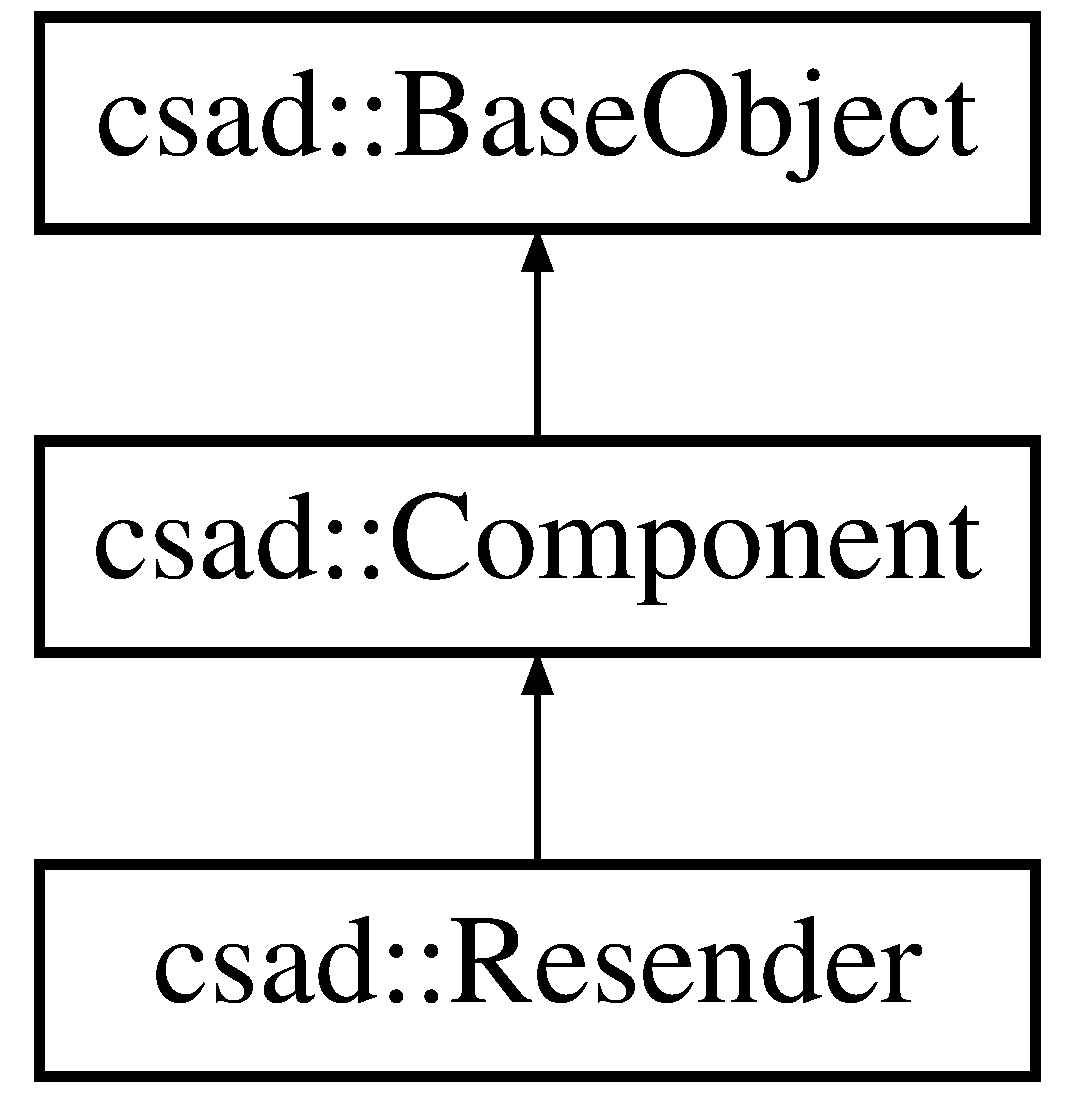
\includegraphics[height=3.000000cm]{classcsad_1_1_resender}
\end{center}
\end{figure}
\subsection*{Public Member Functions}
\begin{DoxyCompactItemize}
\item 
\hypertarget{classcsad_1_1_resender_a5e11724057ba72f430ffe8c630f23ec1}{void $\ast$ \hyperlink{classcsad_1_1_resender_a5e11724057ba72f430ffe8c630f23ec1}{set} (unsigned \-\_\-int32, void $\ast$)}\label{classcsad_1_1_resender_a5e11724057ba72f430ffe8c630f23ec1}

\begin{DoxyCompactList}\small\item\em used for any interface commands. \end{DoxyCompactList}\end{DoxyCompactItemize}
\subsection*{Additional Inherited Members}


\subsection{Detailed Description}
\hyperlink{classcsad_1_1_resender}{Resender} -\/ the component that redirects all events of the specified object. 

\begin{DoxySeeAlso}{See Also}
\hyperlink{group__core}{csad\-: core} 
\end{DoxySeeAlso}

\hypertarget{classcsad_1_1_scene}{\section{csad\-:\-:Scene Class Reference}
\label{classcsad_1_1_scene}\index{csad\-::\-Scene@{csad\-::\-Scene}}
}


\hyperlink{classcsad_1_1_scene}{Scene} -\/ environment objects that belongs to the Manager \hyperlink{classcsad_1_1_graph}{Graph}.  


Inheritance diagram for csad\-:\-:Scene\-:\begin{figure}[H]
\begin{center}
\leavevmode
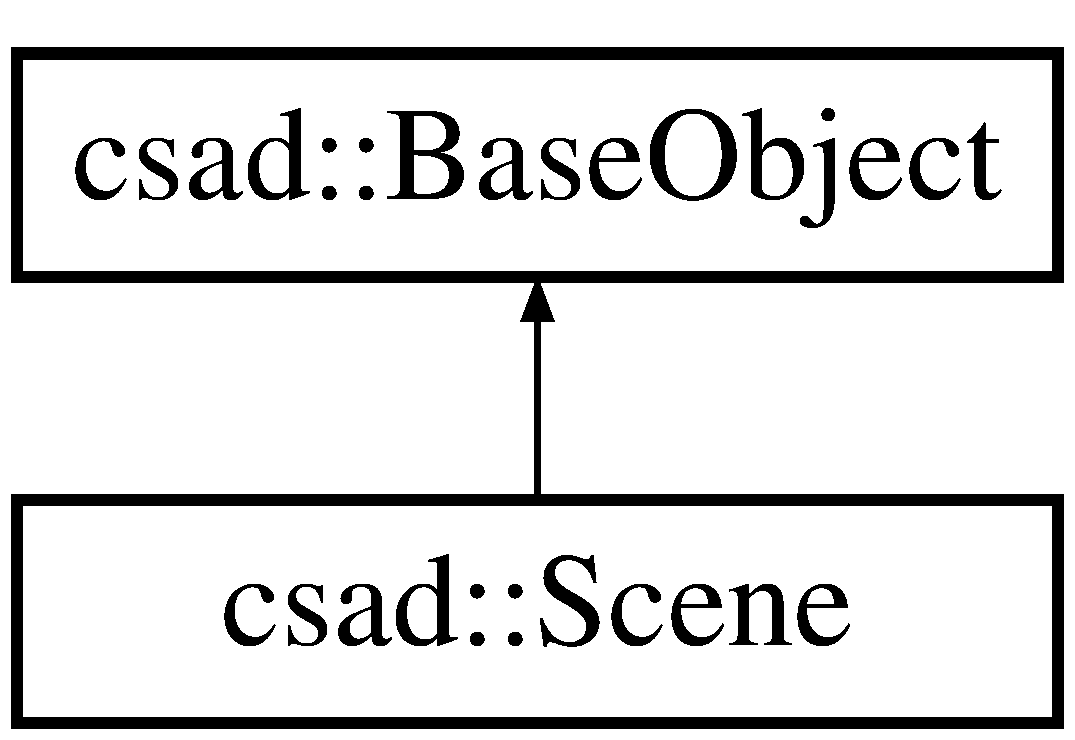
\includegraphics[height=2.000000cm]{classcsad_1_1_scene}
\end{center}
\end{figure}
\subsection*{Public Member Functions}
\begin{DoxyCompactItemize}
\item 
\hypertarget{classcsad_1_1_scene_a10eb8937e7d0ad94681ed9eaa2b8d16c}{\-\_\-\-F\-O\-R\-C\-E\-I\-N\-L\-I\-N\-E bool \hyperlink{classcsad_1_1_scene_a10eb8937e7d0ad94681ed9eaa2b8d16c}{active} ()}\label{classcsad_1_1_scene_a10eb8937e7d0ad94681ed9eaa2b8d16c}

\begin{DoxyCompactList}\small\item\em State of action events. \end{DoxyCompactList}\item 
\hypertarget{classcsad_1_1_scene_aa9b6f21487e82e009d8dd387f238607a}{C\-S\-A\-D\-\_\-\-A\-P\-I \hyperlink{classcsad_1_1_camera}{Camera} $\ast$ \hyperlink{classcsad_1_1_scene_aa9b6f21487e82e009d8dd387f238607a}{create\-Camera} (char $\ast$name, \hyperlink{classcsad_1_1_transform}{Transform} $\ast$parent=0)}\label{classcsad_1_1_scene_aa9b6f21487e82e009d8dd387f238607a}

\begin{DoxyCompactList}\small\item\em creates the camera object, and returns it to the component. \end{DoxyCompactList}\item 
\hypertarget{classcsad_1_1_scene_a904bf3332f4aea7dd4fd62b446309c9a}{C\-S\-A\-D\-\_\-\-A\-P\-I \hyperlink{classcsad_1_1_camera}{Camera} $\ast$ \hyperlink{classcsad_1_1_scene_a904bf3332f4aea7dd4fd62b446309c9a}{create\-Camera} (const char $\ast$name=\char`\"{}\char`\"{}, \hyperlink{classcsad_1_1_transform}{Transform} $\ast$parent=0)}\label{classcsad_1_1_scene_a904bf3332f4aea7dd4fd62b446309c9a}

\begin{DoxyCompactList}\small\item\em creates the camera object, and returns it to the component, with out of name. \end{DoxyCompactList}\item 
\hypertarget{classcsad_1_1_scene_ae1c3f28c9d411628e3b619d0aa04e7be}{C\-S\-A\-D\-\_\-\-A\-P\-I \hyperlink{classcsad_1_1_transform}{Transform} $\ast$ \hyperlink{classcsad_1_1_scene_ae1c3f28c9d411628e3b619d0aa04e7be}{create\-Transform} (char $\ast$name, \hyperlink{classcsad_1_1_transform}{Transform} $\ast$parent=0)}\label{classcsad_1_1_scene_ae1c3f28c9d411628e3b619d0aa04e7be}

\begin{DoxyCompactList}\small\item\em creates the object position. \end{DoxyCompactList}\item 
\hypertarget{classcsad_1_1_scene_a78ce909788631685692501979b0e46bd}{C\-S\-A\-D\-\_\-\-A\-P\-I \hyperlink{classcsad_1_1_transform}{Transform} $\ast$ \hyperlink{classcsad_1_1_scene_a78ce909788631685692501979b0e46bd}{create\-Transform} (const char $\ast$name=\char`\"{}\char`\"{}, \hyperlink{classcsad_1_1_transform}{Transform} $\ast$parent=0)}\label{classcsad_1_1_scene_a78ce909788631685692501979b0e46bd}

\begin{DoxyCompactList}\small\item\em creates the object position, with out of name. \end{DoxyCompactList}\item 
\hypertarget{classcsad_1_1_scene_a48c5a40cad1ba71ae8400b621917a4d5}{C\-S\-A\-D\-\_\-\-A\-P\-I void \hyperlink{classcsad_1_1_scene_a48c5a40cad1ba71ae8400b621917a4d5}{detach\-Object} (\hyperlink{classcsad_1_1_transform}{Transform} $\ast$transform)}\label{classcsad_1_1_scene_a48c5a40cad1ba71ae8400b621917a4d5}

\begin{DoxyCompactList}\small\item\em detach current object position. \end{DoxyCompactList}\item 
\hypertarget{classcsad_1_1_scene_a816697937e32ba2a52d23ff641ee94c3}{C\-S\-A\-D\-\_\-\-A\-P\-I \hyperlink{classcsad_1_1_camera}{Camera} $\ast$ \hyperlink{classcsad_1_1_scene_a816697937e32ba2a52d23ff641ee94c3}{get\-Camera} (char $\ast$name)}\label{classcsad_1_1_scene_a816697937e32ba2a52d23ff641ee94c3}

\begin{DoxyCompactList}\small\item\em returns the camera component. \end{DoxyCompactList}\item 
\hypertarget{classcsad_1_1_scene_a3f600e717cfb1a27201f9b86b7e9c5c3}{\-\_\-\-F\-O\-R\-C\-E\-I\-N\-L\-I\-N\-E \hyperlink{classbt_1_1_map_name}{Objects\-List} \& \hyperlink{classcsad_1_1_scene_a3f600e717cfb1a27201f9b86b7e9c5c3}{get\-Map\-Objects} ()}\label{classcsad_1_1_scene_a3f600e717cfb1a27201f9b86b7e9c5c3}

\begin{DoxyCompactList}\small\item\em returns a named list of objects. \end{DoxyCompactList}\item 
\hypertarget{classcsad_1_1_scene_a1c83dad87a993877e9f083a64904626a}{C\-S\-A\-D\-\_\-\-A\-P\-I const char $\ast$ \hyperlink{classcsad_1_1_scene_a1c83dad87a993877e9f083a64904626a}{get\-Name} ()}\label{classcsad_1_1_scene_a1c83dad87a993877e9f083a64904626a}

\begin{DoxyCompactList}\small\item\em return scene name \end{DoxyCompactList}\item 
\hypertarget{classcsad_1_1_scene_a3986aa8cd7601b486511a50d412b7499}{\-\_\-\-F\-O\-R\-C\-E\-I\-N\-L\-I\-N\-E \hyperlink{classcsad_1_1_transform}{Transform} $\ast$ \hyperlink{classcsad_1_1_scene_a3986aa8cd7601b486511a50d412b7499}{get\-Root} ()}\label{classcsad_1_1_scene_a3986aa8cd7601b486511a50d412b7499}

\begin{DoxyCompactList}\small\item\em returns the root object. \end{DoxyCompactList}\item 
\hypertarget{classcsad_1_1_scene_a369a702aaa81d4456d065fed75dc10a1}{C\-S\-A\-D\-\_\-\-A\-P\-I \hyperlink{classcsad_1_1_transform}{Transform} $\ast$ \hyperlink{classcsad_1_1_scene_a369a702aaa81d4456d065fed75dc10a1}{get\-Transform} (char $\ast$name)}\label{classcsad_1_1_scene_a369a702aaa81d4456d065fed75dc10a1}

\begin{DoxyCompactList}\small\item\em restores the dependent object by name. \end{DoxyCompactList}\item 
\hypertarget{classcsad_1_1_scene_a400941902309674ff39dcf495555f7a6}{C\-S\-A\-D\-\_\-\-A\-P\-I void $\ast$ \hyperlink{classcsad_1_1_scene_a400941902309674ff39dcf495555f7a6}{set} (unsigned \-\_\-int32, void $\ast$)}\label{classcsad_1_1_scene_a400941902309674ff39dcf495555f7a6}

\begin{DoxyCompactList}\small\item\em used for any interface commands. \end{DoxyCompactList}\item 
\hypertarget{classcsad_1_1_scene_af7b981c31cdb952850600a7e08a9d643}{C\-S\-A\-D\-\_\-\-A\-P\-I void \hyperlink{classcsad_1_1_scene_af7b981c31cdb952850600a7e08a9d643}{set\-Active} (bool)}\label{classcsad_1_1_scene_af7b981c31cdb952850600a7e08a9d643}

\begin{DoxyCompactList}\small\item\em Activate scene in events. \end{DoxyCompactList}\end{DoxyCompactItemize}
\subsection*{Static Public Member Functions}
\begin{DoxyCompactItemize}
\item 
\hypertarget{classcsad_1_1_scene_abe6a8e0770c95d3865be7b0f120d664a}{static \hyperlink{classcsad_1_1_scene}{Scene} $\ast$ \hyperlink{classcsad_1_1_scene_abe6a8e0770c95d3865be7b0f120d664a}{get\-Default} ()}\label{classcsad_1_1_scene_abe6a8e0770c95d3865be7b0f120d664a}

\begin{DoxyCompactList}\small\item\em the active scene \end{DoxyCompactList}\end{DoxyCompactItemize}
\subsection*{Additional Inherited Members}


\subsection{Detailed Description}
\hyperlink{classcsad_1_1_scene}{Scene} -\/ environment objects that belongs to the Manager \hyperlink{classcsad_1_1_graph}{Graph}. 

The hierarchical model consisting of objects \hyperlink{classcsad_1_1_transform}{Transform}.

For description in the configuration\-: \begin{DoxyVerb}  <Scene name="the name of the scene">
  ... internal objects ...
  </Scene>
\end{DoxyVerb}


\begin{DoxySeeAlso}{See Also}
\hyperlink{classcsad_1_1_graph}{Graph}, \hyperlink{group__scene}{csad\-: scene}. 
\end{DoxySeeAlso}

\hypertarget{classcsad_1_1_scene_component}{\section{csad\-:\-:Scene\-Component Class Reference}
\label{classcsad_1_1_scene_component}\index{csad\-::\-Scene\-Component@{csad\-::\-Scene\-Component}}
}


\hyperlink{classcsad_1_1_scene_component}{Scene\-Component} -\/ a component is a unique part of the object may not have a name, and to exist independently.  


Inheritance diagram for csad\-:\-:Scene\-Component\-:\begin{figure}[H]
\begin{center}
\leavevmode
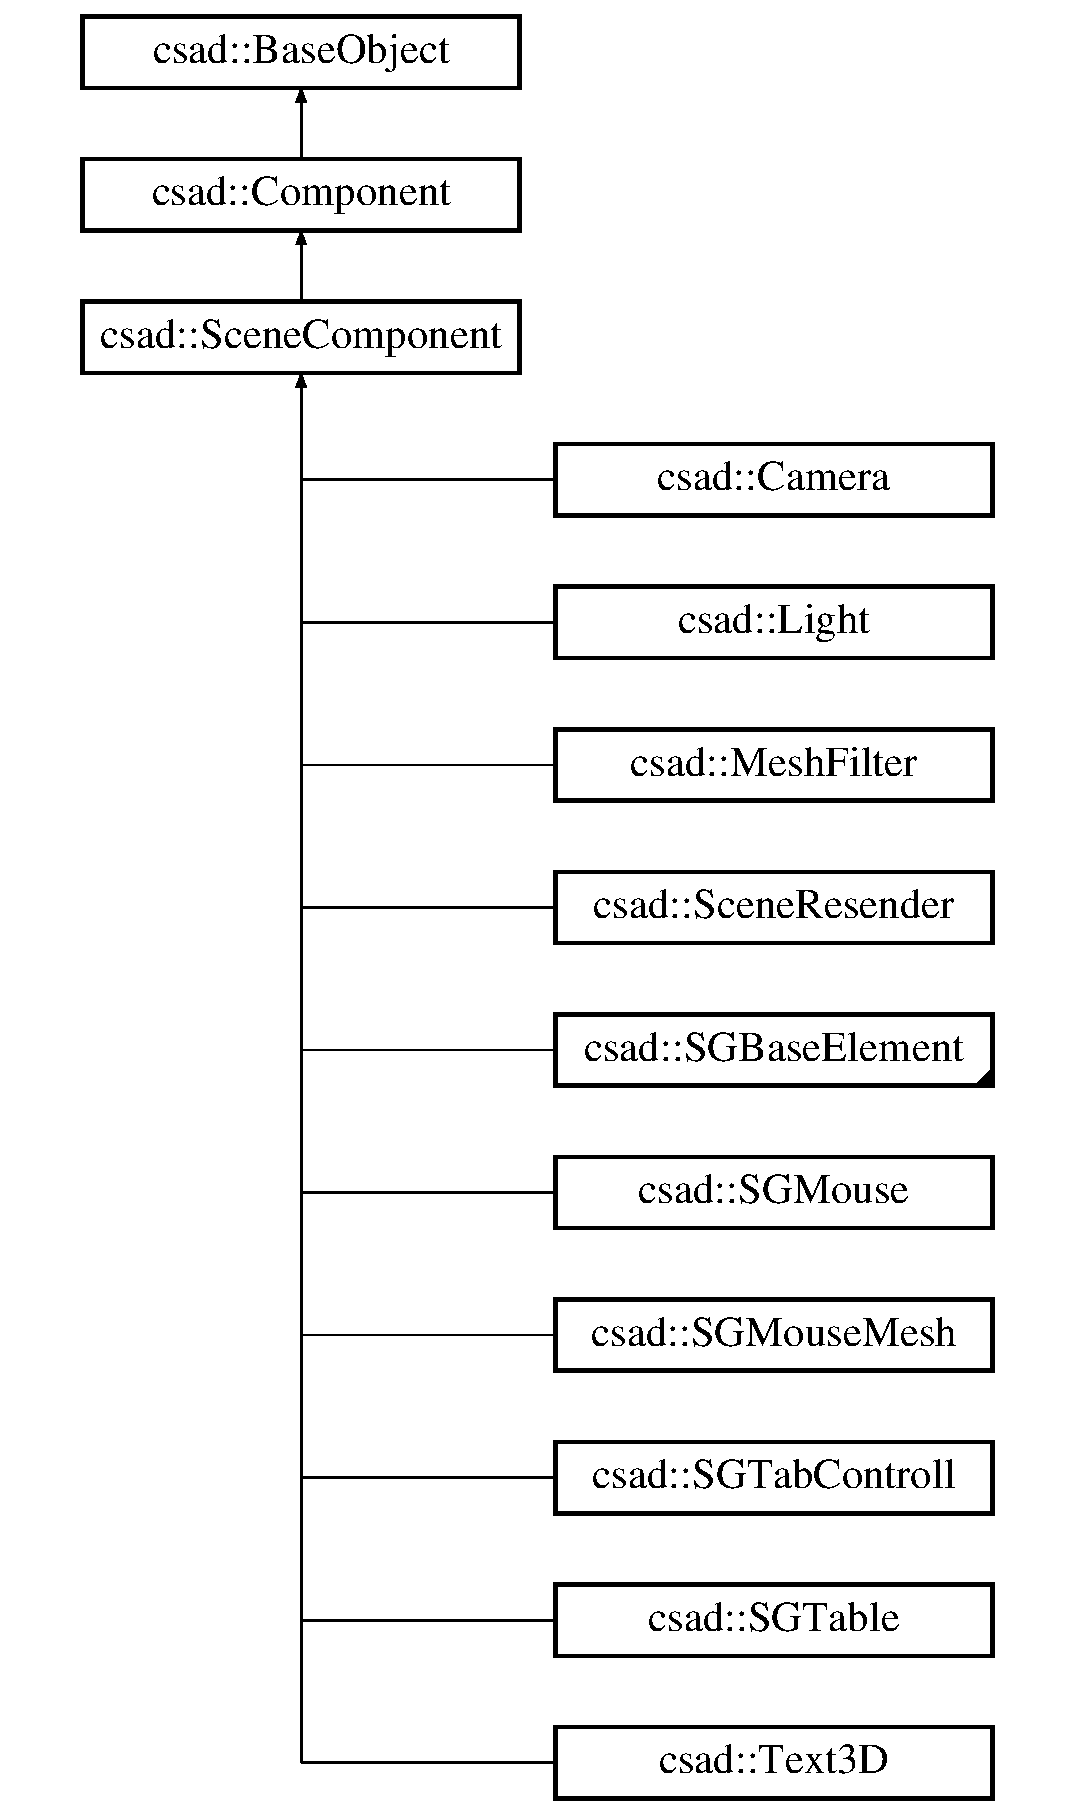
\includegraphics[height=12.000000cm]{classcsad_1_1_scene_component}
\end{center}
\end{figure}
\subsection*{Public Member Functions}
\begin{DoxyCompactItemize}
\item 
\hypertarget{classcsad_1_1_scene_component_aa80f5d0eeb1f01852db3c89dc65ba7d6}{{\footnotesize template$<$typename T $>$ }\\\-\_\-\-F\-O\-R\-C\-E\-I\-N\-L\-I\-N\-E T $\ast$ \hyperlink{classcsad_1_1_scene_component_aa80f5d0eeb1f01852db3c89dc65ba7d6}{add\-Component} ()}\label{classcsad_1_1_scene_component_aa80f5d0eeb1f01852db3c89dc65ba7d6}

\begin{DoxyCompactList}\small\item\em Add component of the specified type in the container if this component already exists, returns available. \end{DoxyCompactList}\item 
\hypertarget{classcsad_1_1_scene_component_a569b1faf246b9e9866ecab9d6c875988}{{\footnotesize template$<$typename T $>$ }\\\-\_\-\-F\-O\-R\-C\-E\-I\-N\-L\-I\-N\-E T $\ast$ \hyperlink{classcsad_1_1_scene_component_a569b1faf246b9e9866ecab9d6c875988}{get\-Component} ()}\label{classcsad_1_1_scene_component_a569b1faf246b9e9866ecab9d6c875988}

\begin{DoxyCompactList}\small\item\em Returns the component of the given type, if it is not in a container returns 0. \end{DoxyCompactList}\item 
\hypertarget{classcsad_1_1_scene_component_a5908ca4554e6f0796614ba97a71c4662}{C\-S\-A\-D\-\_\-\-A\-P\-I \hyperlink{classcsad_1_1_transform}{Transform} $\ast$ \hyperlink{classcsad_1_1_scene_component_a5908ca4554e6f0796614ba97a71c4662}{get\-Container} ()}\label{classcsad_1_1_scene_component_a5908ca4554e6f0796614ba97a71c4662}

\begin{DoxyCompactList}\small\item\em Returns the container in which the component. \end{DoxyCompactList}\item 
\hypertarget{classcsad_1_1_scene_component_a296e949901de8ba9cd84f88bb0d2629b}{virtual C\-S\-A\-D\-\_\-\-A\-P\-I void \hyperlink{classcsad_1_1_scene_component_a296e949901de8ba9cd84f88bb0d2629b}{prepare} ()}\label{classcsad_1_1_scene_component_a296e949901de8ba9cd84f88bb0d2629b}

\begin{DoxyCompactList}\small\item\em The event is called during the preparation stage. \end{DoxyCompactList}\item 
\hypertarget{classcsad_1_1_scene_component_ac0e685f758cbbeb8b348e7675f7c09bd}{virtual C\-S\-A\-D\-\_\-\-A\-P\-I void \hyperlink{classcsad_1_1_scene_component_ac0e685f758cbbeb8b348e7675f7c09bd}{render} ()}\label{classcsad_1_1_scene_component_ac0e685f758cbbeb8b348e7675f7c09bd}

\begin{DoxyCompactList}\small\item\em The event is called during the rendering of the model. \end{DoxyCompactList}\item 
\hypertarget{classcsad_1_1_scene_component_a79ae2a1caa07c798301566d4680097d2}{virtual C\-S\-A\-D\-\_\-\-A\-P\-I void \hyperlink{classcsad_1_1_scene_component_a79ae2a1caa07c798301566d4680097d2}{select} ()}\label{classcsad_1_1_scene_component_a79ae2a1caa07c798301566d4680097d2}

\begin{DoxyCompactList}\small\item\em The event is called during handling of a choice of object -\/ crossing with ray. \end{DoxyCompactList}\end{DoxyCompactItemize}
\subsection*{Additional Inherited Members}


\subsection{Detailed Description}
\hyperlink{classcsad_1_1_scene_component}{Scene\-Component} -\/ a component is a unique part of the object may not have a name, and to exist independently. 

The component has a pointer to the container to which he belongs.

\begin{DoxySeeAlso}{See Also}
\hyperlink{group__scene}{csad\-: scene} 
\end{DoxySeeAlso}

\hypertarget{classcsad_1_1_scene_resender}{\section{csad\-:\-:Scene\-Resender Class Reference}
\label{classcsad_1_1_scene_resender}\index{csad\-::\-Scene\-Resender@{csad\-::\-Scene\-Resender}}
}


\hyperlink{classcsad_1_1_scene_resender}{Scene\-Resender} -\/ the component that redirects all events of the specified object.  


Inheritance diagram for csad\-:\-:Scene\-Resender\-:\begin{figure}[H]
\begin{center}
\leavevmode
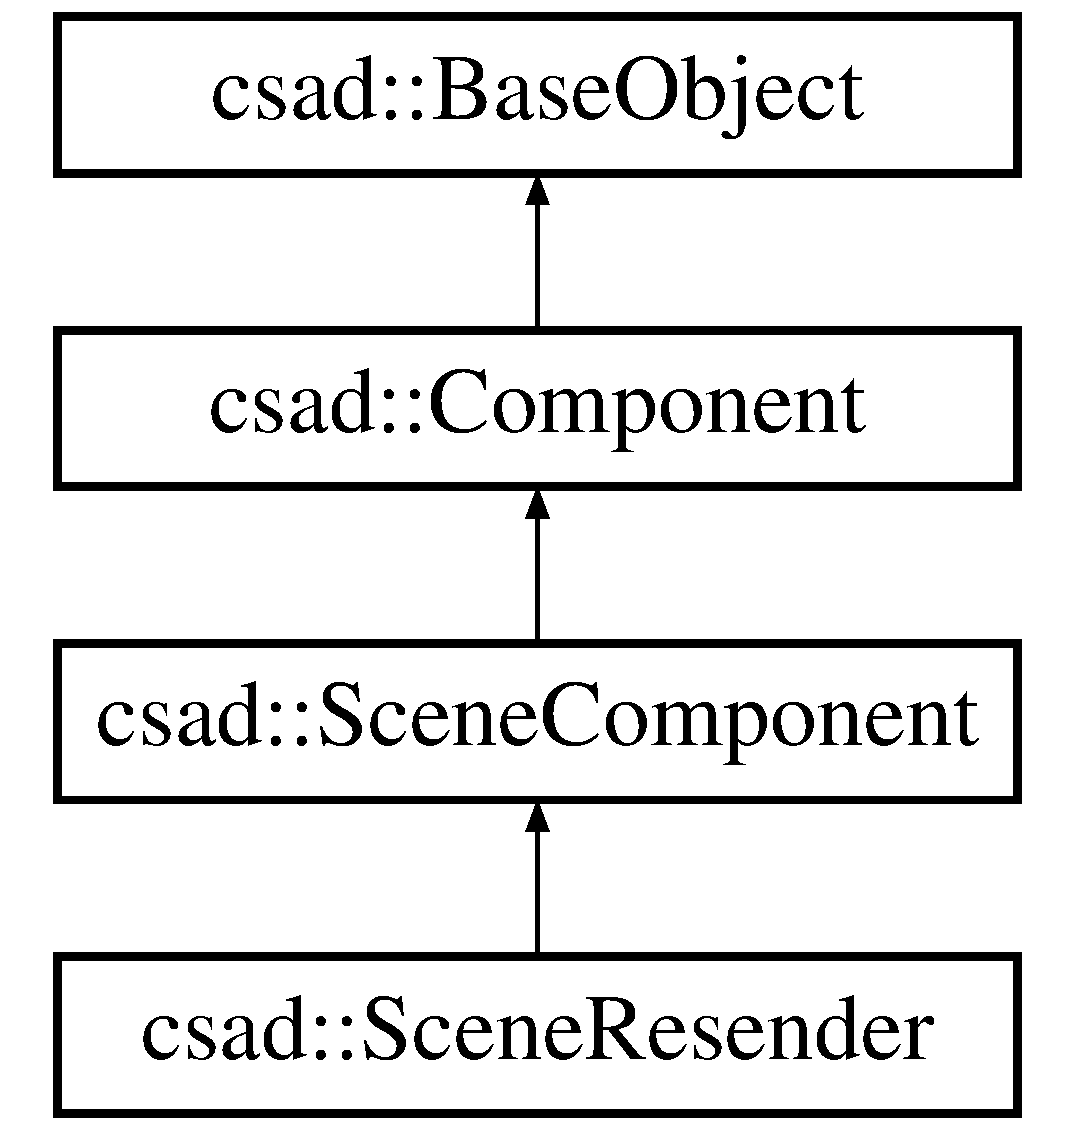
\includegraphics[height=4.000000cm]{classcsad_1_1_scene_resender}
\end{center}
\end{figure}
\subsection*{Public Member Functions}
\begin{DoxyCompactItemize}
\item 
\hypertarget{classcsad_1_1_scene_resender_a70247fb3c572288274e122315f92a7ec}{C\-S\-A\-D\-\_\-\-A\-P\-I void $\ast$ \hyperlink{classcsad_1_1_scene_resender_a70247fb3c572288274e122315f92a7ec}{set} (unsigned \-\_\-int32, void $\ast$)}\label{classcsad_1_1_scene_resender_a70247fb3c572288274e122315f92a7ec}

\begin{DoxyCompactList}\small\item\em used for any interface commands. \end{DoxyCompactList}\end{DoxyCompactItemize}
\subsection*{Additional Inherited Members}


\subsection{Detailed Description}
\hyperlink{classcsad_1_1_scene_resender}{Scene\-Resender} -\/ the component that redirects all events of the specified object. 

\begin{DoxySeeAlso}{See Also}
\hyperlink{group__core}{csad\-: core} 
\end{DoxySeeAlso}

\hypertarget{classcsad_1_1_s_g_base_element}{\section{csad\-:\-:S\-G\-Base\-Element Class Reference}
\label{classcsad_1_1_s_g_base_element}\index{csad\-::\-S\-G\-Base\-Element@{csad\-::\-S\-G\-Base\-Element}}
}


\hyperlink{classcsad_1_1_s_g_base_element}{S\-G\-Base\-Element} -\/ base class for gui elements.  


Inheritance diagram for csad\-:\-:S\-G\-Base\-Element\-:\begin{figure}[H]
\begin{center}
\leavevmode
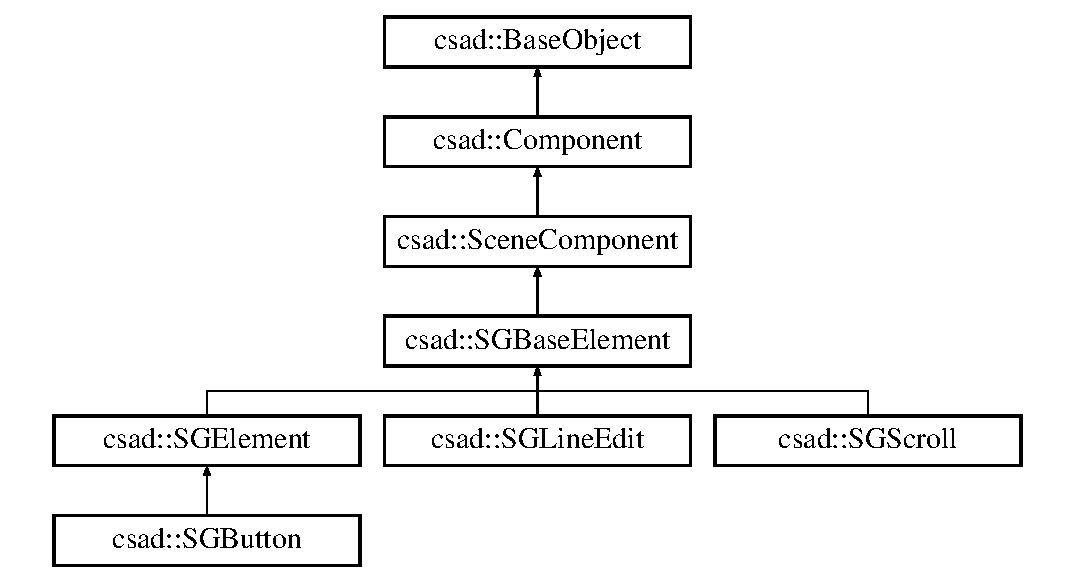
\includegraphics[height=6.000000cm]{classcsad_1_1_s_g_base_element}
\end{center}
\end{figure}
\subsection*{Public Types}
\begin{DoxyCompactItemize}
\item 
enum \hyperlink{classcsad_1_1_s_g_base_element_ab936ff0f0f69ecf8b67d60e53ae30cd0}{State} \{ \\*
\hyperlink{classcsad_1_1_s_g_base_element_ab936ff0f0f69ecf8b67d60e53ae30cd0a92de2f632ce50553c439ccf7be7fb49c}{Normal} = 0x0, 
\hyperlink{classcsad_1_1_s_g_base_element_ab936ff0f0f69ecf8b67d60e53ae30cd0a4f85b7110ba36e6528e4525940bbaa30}{Active} = 0x1, 
\hyperlink{classcsad_1_1_s_g_base_element_ab936ff0f0f69ecf8b67d60e53ae30cd0af0f2e90a5c21acc8ecd2bd39f7f171cd}{Click} = 0x2, 
\hyperlink{classcsad_1_1_s_g_base_element_ab936ff0f0f69ecf8b67d60e53ae30cd0aa2fd3cf9e226675e04ac4f29d20dd9ca}{Disable} = 0x3, 
\\*
\hyperlink{classcsad_1_1_s_g_base_element_ab936ff0f0f69ecf8b67d60e53ae30cd0ac561cea7ffdb2ae25058cb24ac7c0880}{S\-G\-E\-\_\-\-Set} = 0x100
, \hyperlink{classcsad_1_1_s_g_base_element_ab936ff0f0f69ecf8b67d60e53ae30cd0a79b2a0773a4086055a45a40d48023698}{S\-G\-E\-\_\-\-Set\-Button} = 0x0000, 
\hyperlink{classcsad_1_1_s_g_base_element_ab936ff0f0f69ecf8b67d60e53ae30cd0a89cdb6212cdf0cfe4a704ff136ca2630}{S\-G\-E\-\_\-\-Set\-Select} = 0x1000, 
\hyperlink{classcsad_1_1_s_g_base_element_ab936ff0f0f69ecf8b67d60e53ae30cd0afa0d9a05aa79ae656a43b7398e928604}{S\-G\-E\-\_\-\-Set\-Switch} = 0x2000, 
\\*
\hyperlink{classcsad_1_1_s_g_base_element_ab936ff0f0f69ecf8b67d60e53ae30cd0a6f0bf457081d2bd938f3ba2ed164d42d}{S\-G\-E\-\_\-\-Set\-Open} = 0x3000, 
\hyperlink{classcsad_1_1_s_g_base_element_ab936ff0f0f69ecf8b67d60e53ae30cd0a89e7d86b338fdc3a88a1fe7f94481766}{S\-G\-E\-\_\-\-Opened} = 0x10000
, \hyperlink{classcsad_1_1_s_g_base_element_ab936ff0f0f69ecf8b67d60e53ae30cd0a202751683618959b30a6f50cbbe15b7a}{S\-G\-E\-\_\-\-Vertical} = 0x00000, 
\hyperlink{classcsad_1_1_s_g_base_element_ab936ff0f0f69ecf8b67d60e53ae30cd0a8a69f16afd37f363140bde77ea1de227}{S\-G\-E\-\_\-\-Horisontal} = 0x80000, 
\\*
\hyperlink{classcsad_1_1_s_g_base_element_ab936ff0f0f69ecf8b67d60e53ae30cd0afcbf1e4a77948d4fae4a5ba5e2d751b3}{S\-G\-E\-\_\-\-End} = 0x100000
 \}
\end{DoxyCompactItemize}
\subsection*{Additional Inherited Members}


\subsection{Detailed Description}
\hyperlink{classcsad_1_1_s_g_base_element}{S\-G\-Base\-Element} -\/ base class for gui elements. 

\begin{DoxySeeAlso}{See Also}
\hyperlink{classcsad_1_1_s_g_element}{S\-G\-Element}, S\-G\-List\-Element, \hyperlink{group__scenegui}{csad\-: gui} 
\end{DoxySeeAlso}


\subsection{Member Enumeration Documentation}
\hypertarget{classcsad_1_1_s_g_base_element_ab936ff0f0f69ecf8b67d60e53ae30cd0}{\index{csad\-::\-S\-G\-Base\-Element@{csad\-::\-S\-G\-Base\-Element}!State@{State}}
\index{State@{State}!csad::SGBaseElement@{csad\-::\-S\-G\-Base\-Element}}
\subsubsection[{State}]{\setlength{\rightskip}{0pt plus 5cm}enum {\bf csad\-::\-S\-G\-Base\-Element\-::\-State}}}\label{classcsad_1_1_s_g_base_element_ab936ff0f0f69ecf8b67d60e53ae30cd0}
\begin{Desc}
\item[Enumerator]\par
\begin{description}
\index{Normal@{Normal}!csad\-::\-S\-G\-Base\-Element@{csad\-::\-S\-G\-Base\-Element}}\index{csad\-::\-S\-G\-Base\-Element@{csad\-::\-S\-G\-Base\-Element}!Normal@{Normal}}\item[{\em 
\hypertarget{classcsad_1_1_s_g_base_element_ab936ff0f0f69ecf8b67d60e53ae30cd0a92de2f632ce50553c439ccf7be7fb49c}{Normal}\label{classcsad_1_1_s_g_base_element_ab936ff0f0f69ecf8b67d60e53ae30cd0a92de2f632ce50553c439ccf7be7fb49c}
}]not active state \index{Active@{Active}!csad\-::\-S\-G\-Base\-Element@{csad\-::\-S\-G\-Base\-Element}}\index{csad\-::\-S\-G\-Base\-Element@{csad\-::\-S\-G\-Base\-Element}!Active@{Active}}\item[{\em 
\hypertarget{classcsad_1_1_s_g_base_element_ab936ff0f0f69ecf8b67d60e53ae30cd0a4f85b7110ba36e6528e4525940bbaa30}{Active}\label{classcsad_1_1_s_g_base_element_ab936ff0f0f69ecf8b67d60e53ae30cd0a4f85b7110ba36e6528e4525940bbaa30}
}]key active \index{Click@{Click}!csad\-::\-S\-G\-Base\-Element@{csad\-::\-S\-G\-Base\-Element}}\index{csad\-::\-S\-G\-Base\-Element@{csad\-::\-S\-G\-Base\-Element}!Click@{Click}}\item[{\em 
\hypertarget{classcsad_1_1_s_g_base_element_ab936ff0f0f69ecf8b67d60e53ae30cd0af0f2e90a5c21acc8ecd2bd39f7f171cd}{Click}\label{classcsad_1_1_s_g_base_element_ab936ff0f0f69ecf8b67d60e53ae30cd0af0f2e90a5c21acc8ecd2bd39f7f171cd}
}]a key is pressed \index{Disable@{Disable}!csad\-::\-S\-G\-Base\-Element@{csad\-::\-S\-G\-Base\-Element}}\index{csad\-::\-S\-G\-Base\-Element@{csad\-::\-S\-G\-Base\-Element}!Disable@{Disable}}\item[{\em 
\hypertarget{classcsad_1_1_s_g_base_element_ab936ff0f0f69ecf8b67d60e53ae30cd0aa2fd3cf9e226675e04ac4f29d20dd9ca}{Disable}\label{classcsad_1_1_s_g_base_element_ab936ff0f0f69ecf8b67d60e53ae30cd0aa2fd3cf9e226675e04ac4f29d20dd9ca}
}]the item is disabled \index{S\-G\-E\-\_\-\-Set@{S\-G\-E\-\_\-\-Set}!csad\-::\-S\-G\-Base\-Element@{csad\-::\-S\-G\-Base\-Element}}\index{csad\-::\-S\-G\-Base\-Element@{csad\-::\-S\-G\-Base\-Element}!S\-G\-E\-\_\-\-Set@{S\-G\-E\-\_\-\-Set}}\item[{\em 
\hypertarget{classcsad_1_1_s_g_base_element_ab936ff0f0f69ecf8b67d60e53ae30cd0ac561cea7ffdb2ae25058cb24ac7c0880}{S\-G\-E\-\_\-\-Set}\label{classcsad_1_1_s_g_base_element_ab936ff0f0f69ecf8b67d60e53ae30cd0ac561cea7ffdb2ae25058cb24ac7c0880}
}]the item is selected (for a group of buttons) \index{S\-G\-E\-\_\-\-Set\-Button@{S\-G\-E\-\_\-\-Set\-Button}!csad\-::\-S\-G\-Base\-Element@{csad\-::\-S\-G\-Base\-Element}}\index{csad\-::\-S\-G\-Base\-Element@{csad\-::\-S\-G\-Base\-Element}!S\-G\-E\-\_\-\-Set\-Button@{S\-G\-E\-\_\-\-Set\-Button}}\item[{\em 
\hypertarget{classcsad_1_1_s_g_base_element_ab936ff0f0f69ecf8b67d60e53ae30cd0a79b2a0773a4086055a45a40d48023698}{S\-G\-E\-\_\-\-Set\-Button}\label{classcsad_1_1_s_g_base_element_ab936ff0f0f69ecf8b67d60e53ae30cd0a79b2a0773a4086055a45a40d48023698}
}]button mode \index{S\-G\-E\-\_\-\-Set\-Select@{S\-G\-E\-\_\-\-Set\-Select}!csad\-::\-S\-G\-Base\-Element@{csad\-::\-S\-G\-Base\-Element}}\index{csad\-::\-S\-G\-Base\-Element@{csad\-::\-S\-G\-Base\-Element}!S\-G\-E\-\_\-\-Set\-Select@{S\-G\-E\-\_\-\-Set\-Select}}\item[{\em 
\hypertarget{classcsad_1_1_s_g_base_element_ab936ff0f0f69ecf8b67d60e53ae30cd0a89cdb6212cdf0cfe4a704ff136ca2630}{S\-G\-E\-\_\-\-Set\-Select}\label{classcsad_1_1_s_g_base_element_ab936ff0f0f69ecf8b67d60e53ae30cd0a89cdb6212cdf0cfe4a704ff136ca2630}
}]mode \index{S\-G\-E\-\_\-\-Set\-Switch@{S\-G\-E\-\_\-\-Set\-Switch}!csad\-::\-S\-G\-Base\-Element@{csad\-::\-S\-G\-Base\-Element}}\index{csad\-::\-S\-G\-Base\-Element@{csad\-::\-S\-G\-Base\-Element}!S\-G\-E\-\_\-\-Set\-Switch@{S\-G\-E\-\_\-\-Set\-Switch}}\item[{\em 
\hypertarget{classcsad_1_1_s_g_base_element_ab936ff0f0f69ecf8b67d60e53ae30cd0afa0d9a05aa79ae656a43b7398e928604}{S\-G\-E\-\_\-\-Set\-Switch}\label{classcsad_1_1_s_g_base_element_ab936ff0f0f69ecf8b67d60e53ae30cd0afa0d9a05aa79ae656a43b7398e928604}
}]inversion mode \index{S\-G\-E\-\_\-\-Set\-Open@{S\-G\-E\-\_\-\-Set\-Open}!csad\-::\-S\-G\-Base\-Element@{csad\-::\-S\-G\-Base\-Element}}\index{csad\-::\-S\-G\-Base\-Element@{csad\-::\-S\-G\-Base\-Element}!S\-G\-E\-\_\-\-Set\-Open@{S\-G\-E\-\_\-\-Set\-Open}}\item[{\em 
\hypertarget{classcsad_1_1_s_g_base_element_ab936ff0f0f69ecf8b67d60e53ae30cd0a6f0bf457081d2bd938f3ba2ed164d42d}{S\-G\-E\-\_\-\-Set\-Open}\label{classcsad_1_1_s_g_base_element_ab936ff0f0f69ecf8b67d60e53ae30cd0a6f0bf457081d2bd938f3ba2ed164d42d}
}]inversion key mode \index{S\-G\-E\-\_\-\-Opened@{S\-G\-E\-\_\-\-Opened}!csad\-::\-S\-G\-Base\-Element@{csad\-::\-S\-G\-Base\-Element}}\index{csad\-::\-S\-G\-Base\-Element@{csad\-::\-S\-G\-Base\-Element}!S\-G\-E\-\_\-\-Opened@{S\-G\-E\-\_\-\-Opened}}\item[{\em 
\hypertarget{classcsad_1_1_s_g_base_element_ab936ff0f0f69ecf8b67d60e53ae30cd0a89e7d86b338fdc3a88a1fe7f94481766}{S\-G\-E\-\_\-\-Opened}\label{classcsad_1_1_s_g_base_element_ab936ff0f0f69ecf8b67d60e53ae30cd0a89e7d86b338fdc3a88a1fe7f94481766}
}]indicate state \index{S\-G\-E\-\_\-\-Vertical@{S\-G\-E\-\_\-\-Vertical}!csad\-::\-S\-G\-Base\-Element@{csad\-::\-S\-G\-Base\-Element}}\index{csad\-::\-S\-G\-Base\-Element@{csad\-::\-S\-G\-Base\-Element}!S\-G\-E\-\_\-\-Vertical@{S\-G\-E\-\_\-\-Vertical}}\item[{\em 
\hypertarget{classcsad_1_1_s_g_base_element_ab936ff0f0f69ecf8b67d60e53ae30cd0a202751683618959b30a6f50cbbe15b7a}{S\-G\-E\-\_\-\-Vertical}\label{classcsad_1_1_s_g_base_element_ab936ff0f0f69ecf8b67d60e53ae30cd0a202751683618959b30a6f50cbbe15b7a}
}]режим ориентации вертикальный \index{S\-G\-E\-\_\-\-Horisontal@{S\-G\-E\-\_\-\-Horisontal}!csad\-::\-S\-G\-Base\-Element@{csad\-::\-S\-G\-Base\-Element}}\index{csad\-::\-S\-G\-Base\-Element@{csad\-::\-S\-G\-Base\-Element}!S\-G\-E\-\_\-\-Horisontal@{S\-G\-E\-\_\-\-Horisontal}}\item[{\em 
\hypertarget{classcsad_1_1_s_g_base_element_ab936ff0f0f69ecf8b67d60e53ae30cd0a8a69f16afd37f363140bde77ea1de227}{S\-G\-E\-\_\-\-Horisontal}\label{classcsad_1_1_s_g_base_element_ab936ff0f0f69ecf8b67d60e53ae30cd0a8a69f16afd37f363140bde77ea1de227}
}]режим ориентации горизонтальный \index{S\-G\-E\-\_\-\-End@{S\-G\-E\-\_\-\-End}!csad\-::\-S\-G\-Base\-Element@{csad\-::\-S\-G\-Base\-Element}}\index{csad\-::\-S\-G\-Base\-Element@{csad\-::\-S\-G\-Base\-Element}!S\-G\-E\-\_\-\-End@{S\-G\-E\-\_\-\-End}}\item[{\em 
\hypertarget{classcsad_1_1_s_g_base_element_ab936ff0f0f69ecf8b67d60e53ae30cd0afcbf1e4a77948d4fae4a5ba5e2d751b3}{S\-G\-E\-\_\-\-End}\label{classcsad_1_1_s_g_base_element_ab936ff0f0f69ecf8b67d60e53ae30cd0afcbf1e4a77948d4fae4a5ba5e2d751b3}
}]is event end \end{description}
\end{Desc}

\hypertarget{classcsad_1_1_s_g_button}{\section{csad\-:\-:S\-G\-Button Class Reference}
\label{classcsad_1_1_s_g_button}\index{csad\-::\-S\-G\-Button@{csad\-::\-S\-G\-Button}}
}


\hyperlink{classcsad_1_1_s_g_button}{S\-G\-Button} -\/ component, which is the controller buttons, defines the characteristics of the image and manages events.  


Inheritance diagram for csad\-:\-:S\-G\-Button\-:\begin{figure}[H]
\begin{center}
\leavevmode
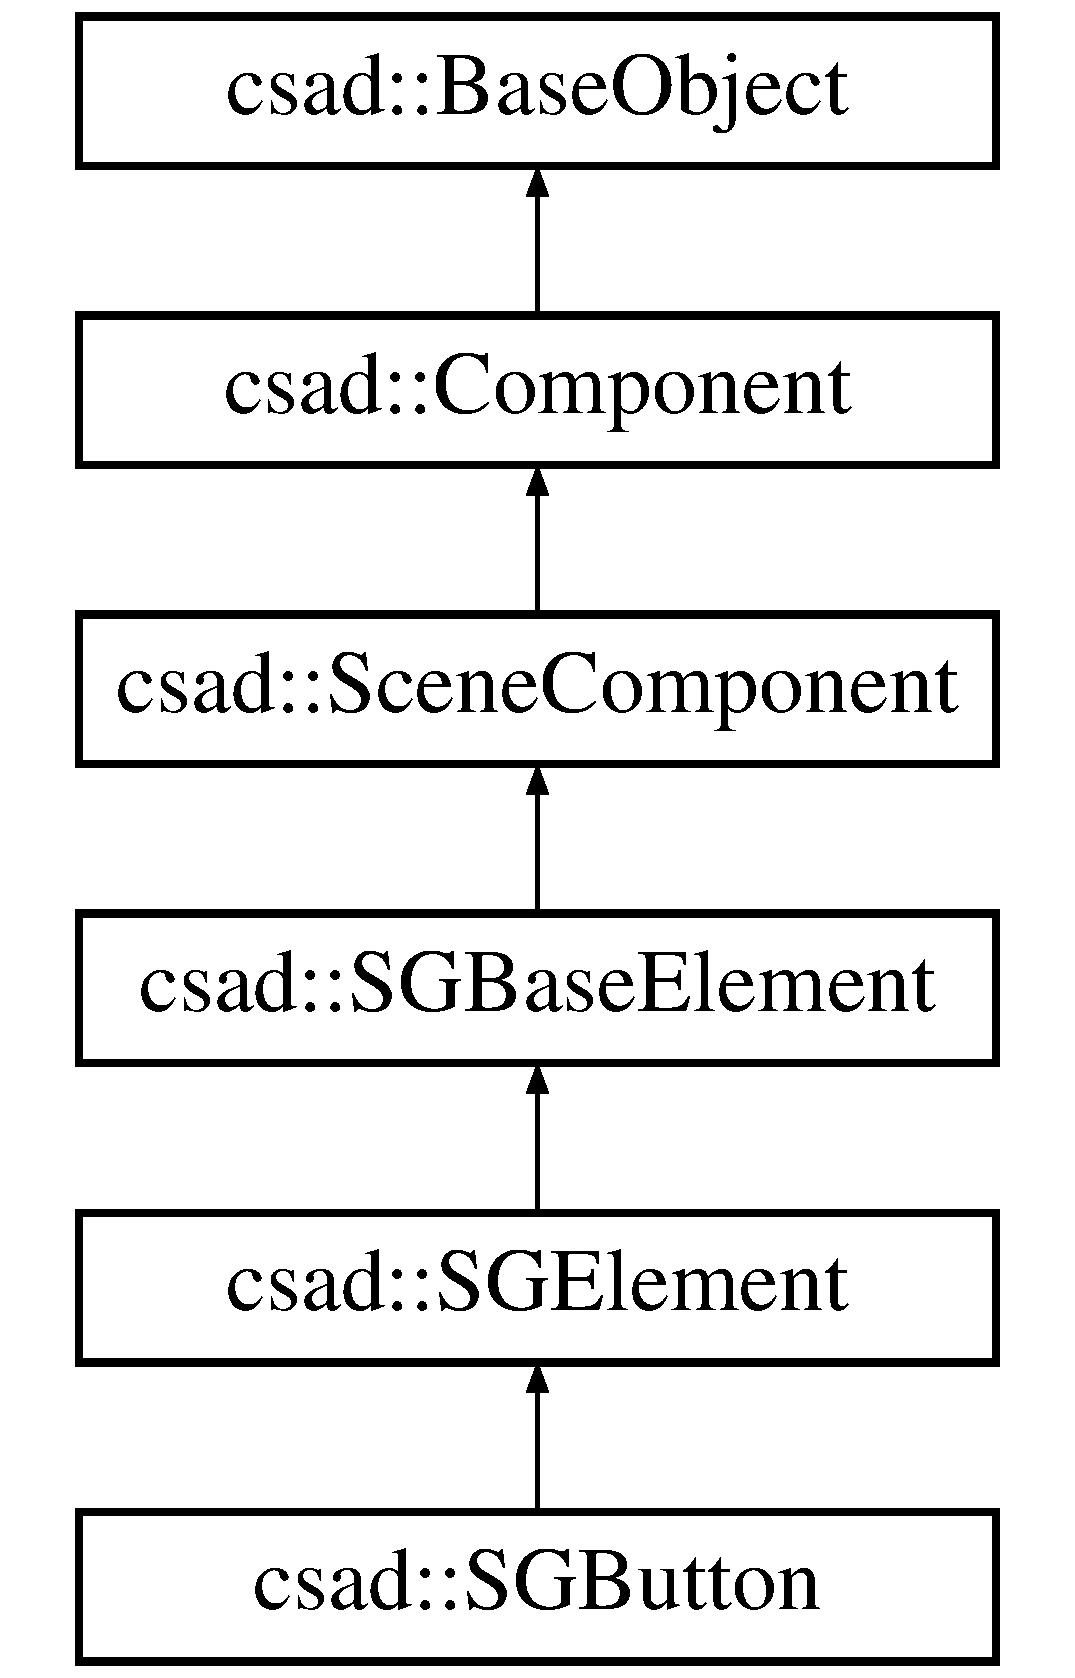
\includegraphics[height=6.000000cm]{classcsad_1_1_s_g_button}
\end{center}
\end{figure}
\subsection*{Public Member Functions}
\begin{DoxyCompactItemize}
\item 
\hypertarget{classcsad_1_1_s_g_button_a7b51182ae7fbbd76e887cf6fed241f83}{C\-S\-A\-D\-\_\-\-A\-P\-I void $\ast$ \hyperlink{classcsad_1_1_s_g_button_a7b51182ae7fbbd76e887cf6fed241f83}{set} (unsigned \-\_\-int32, void $\ast$)}\label{classcsad_1_1_s_g_button_a7b51182ae7fbbd76e887cf6fed241f83}

\begin{DoxyCompactList}\small\item\em used for any interface commands. \end{DoxyCompactList}\end{DoxyCompactItemize}
\subsection*{Additional Inherited Members}


\subsection{Detailed Description}
\hyperlink{classcsad_1_1_s_g_button}{S\-G\-Button} -\/ component, which is the controller buttons, defines the characteristics of the image and manages events. 

To handle events keys, you must install a handler recipient using the \hyperlink{classcsad_1_1_s_g_element_a1a8aaf98a4fb6960e00365000b44bff9}{S\-G\-Button\-::set\-Receiver}. Event processing is performed in the method \hyperlink{classcsad_1_1_base_object_aa8d3a855874527b14a5c56f629789b1f}{Base\-Object\-::set} when the parameter id==\hyperlink{classcsad_1_1_base_object_a27d9db492c1a385aa4086da1824e2737a1ad754d1312e455b8585419a33bba1bf}{Base\-Object\-::\-S\-E\-L\-E\-C\-T}, and the second parameter contains a pointer to the component type \hyperlink{classcsad_1_1_s_g_button}{S\-G\-Button}. This can be any object of a class inherited from the \hyperlink{classcsad_1_1_base_object}{Base\-Object} class or his descendants.

For description in the configuration\-: \begin{DoxyVerb}  <Scene name="myKeyScene">
    <Transform name="name of the button" pos="0 0 0" scale="0.1 0.1 0.1">
      <SGButton size="0.1 0.05 0" text="key text" style="buttonstyle"/>
    </Transform>
  </Scene>
\end{DoxyVerb}


\begin{DoxySeeAlso}{See Also}
\hyperlink{group__scenegui}{csad\-: gui}, \hyperlink{classcsad_1_1_style}{Style}, \hyperlink{classcsad_1_1_text_style}{Text\-Style}, \hyperlink{classcsad_1_1_s_g_button_style}{S\-G\-Button\-Style}, \hyperlink{classcsad_1_1_base_object}{Base\-Object} 
\end{DoxySeeAlso}

\hypertarget{classcsad_1_1_s_g_button_style}{\section{csad\-:\-:S\-G\-Button\-Style Class Reference}
\label{classcsad_1_1_s_g_button_style}\index{csad\-::\-S\-G\-Button\-Style@{csad\-::\-S\-G\-Button\-Style}}
}


\hyperlink{classcsad_1_1_s_g_button_style}{S\-G\-Button\-Style} -\/ component containing the settings button States.  




Inherits csad\-::\-S\-G\-Style.

\subsection*{Public Member Functions}
\begin{DoxyCompactItemize}
\item 
\hypertarget{classcsad_1_1_s_g_button_style_ae45d6aca454954567f289daa3d0a69e8}{C\-S\-A\-D\-\_\-\-A\-P\-I void $\ast$ \hyperlink{classcsad_1_1_s_g_button_style_ae45d6aca454954567f289daa3d0a69e8}{set} (unsigned \-\_\-int32, void $\ast$)}\label{classcsad_1_1_s_g_button_style_ae45d6aca454954567f289daa3d0a69e8}

\begin{DoxyCompactList}\small\item\em used for any interface commands. \end{DoxyCompactList}\end{DoxyCompactItemize}
\subsection*{Additional Inherited Members}


\subsection{Detailed Description}
\hyperlink{classcsad_1_1_s_g_button_style}{S\-G\-Button\-Style} -\/ component containing the settings button States. 

For description in the configuration\-: \begin{DoxyVerb}  <Style name="buttonstyle">
     <SGButtonStyle normal="butmatnormal" active="butmatactive" click="butmatclick"/>
     <SGButtonStyle normal_text="textmatnormal" normal_text="textmatactive" normal_text="textmatclick"/>
  </Style>
\end{DoxyVerb}


\begin{DoxySeeAlso}{See Also}
\hyperlink{group__scenegui}{csad\-: gui}, \hyperlink{classcsad_1_1_s_g_button}{S\-G\-Button} 
\end{DoxySeeAlso}

\hypertarget{classcsad_1_1_s_g_element}{\section{csad\-:\-:S\-G\-Element Class Reference}
\label{classcsad_1_1_s_g_element}\index{csad\-::\-S\-G\-Element@{csad\-::\-S\-G\-Element}}
}


\hyperlink{classcsad_1_1_s_g_element}{S\-G\-Element} -\/ component, which is the action controller, defines the characteristics of the image and manages events.  


Inheritance diagram for csad\-:\-:S\-G\-Element\-:\begin{figure}[H]
\begin{center}
\leavevmode
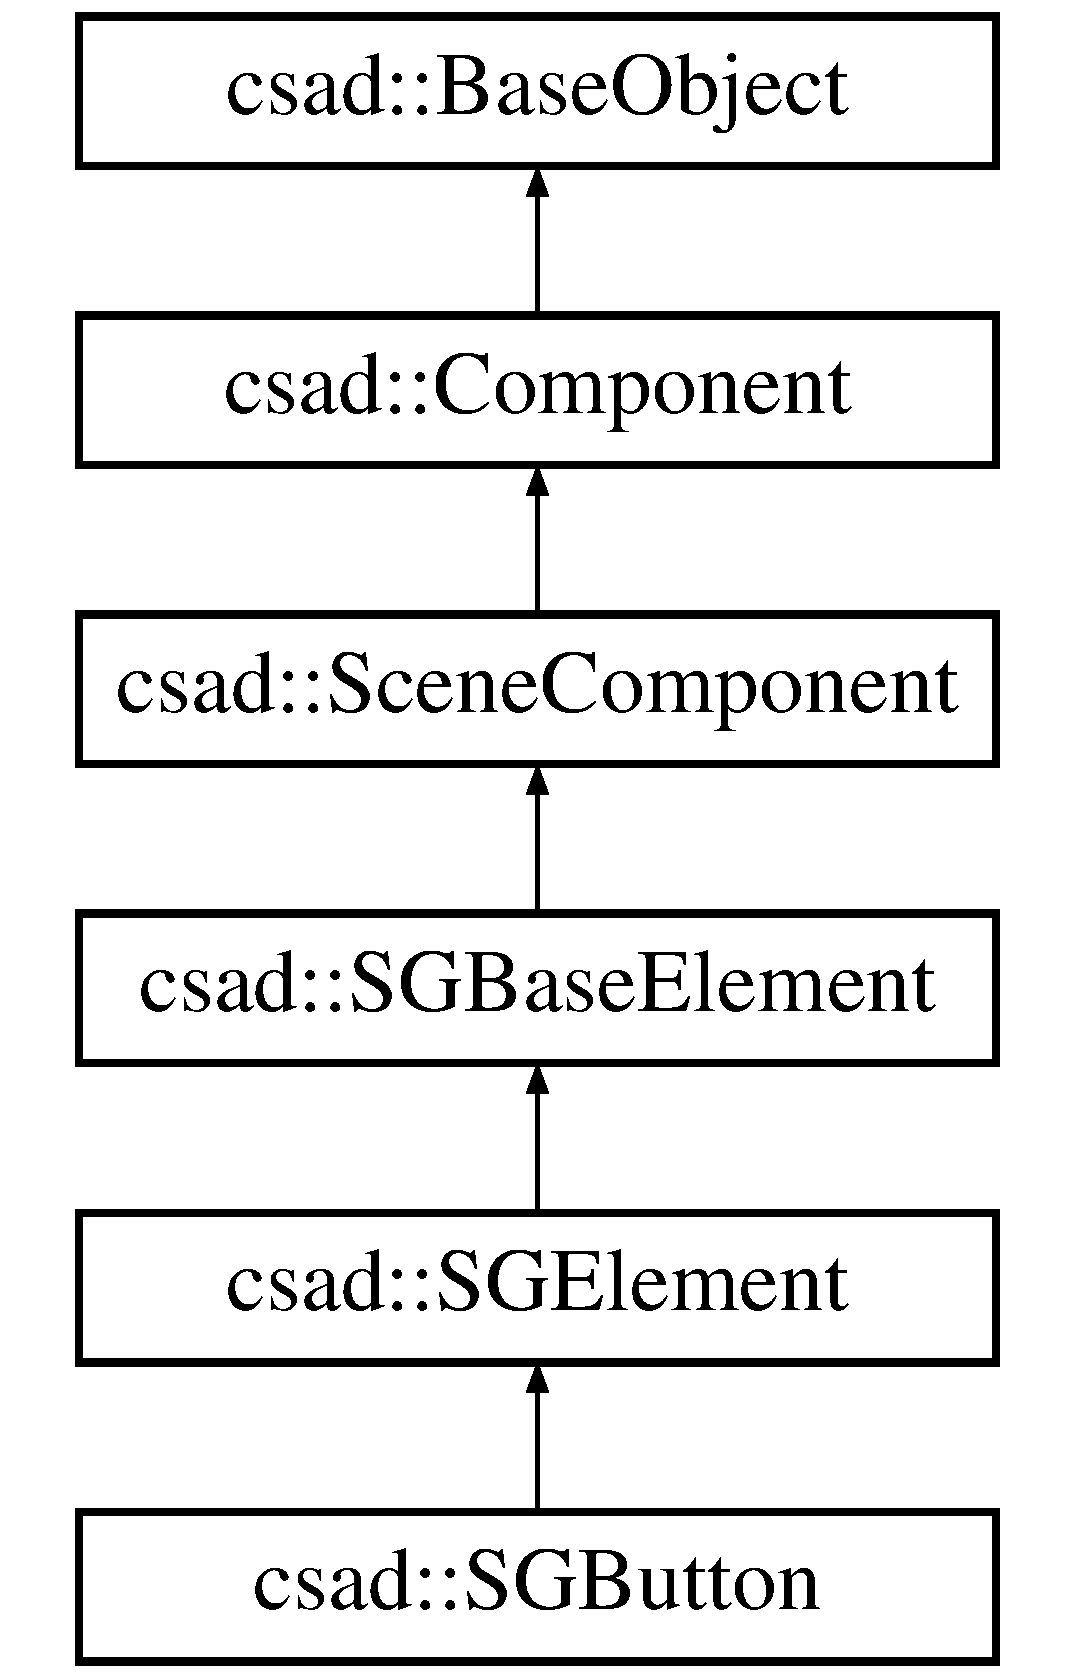
\includegraphics[height=6.000000cm]{classcsad_1_1_s_g_element}
\end{center}
\end{figure}
\subsection*{Public Member Functions}
\begin{DoxyCompactItemize}
\item 
\hypertarget{classcsad_1_1_s_g_element_a1ac3dbf52e5e3b2fca6092724eeeac28}{C\-S\-A\-D\-\_\-\-A\-P\-I const char $\ast$ \hyperlink{classcsad_1_1_s_g_element_a1ac3dbf52e5e3b2fca6092724eeeac28}{get\-Text} ()}\label{classcsad_1_1_s_g_element_a1ac3dbf52e5e3b2fca6092724eeeac28}

\begin{DoxyCompactList}\small\item\em returns the text of the element (components \hyperlink{classcsad_1_1_text3_d}{Text3\-D}) \end{DoxyCompactList}\item 
\hypertarget{classcsad_1_1_s_g_element_abb1870688c04a966bf5b9761821408ed}{\-\_\-\-F\-O\-R\-C\-E\-I\-N\-L\-I\-N\-E bool \hyperlink{classcsad_1_1_s_g_element_abb1870688c04a966bf5b9761821408ed}{is\-Active} ()}\label{classcsad_1_1_s_g_element_abb1870688c04a966bf5b9761821408ed}

\begin{DoxyCompactList}\small\item\em Returns true if the installed state of the Active. \end{DoxyCompactList}\item 
\hypertarget{classcsad_1_1_s_g_element_a082c989cb5c2c68f097a74e6bfe5970a}{\-\_\-\-F\-O\-R\-C\-E\-I\-N\-L\-I\-N\-E bool \hyperlink{classcsad_1_1_s_g_element_a082c989cb5c2c68f097a74e6bfe5970a}{is\-Click} ()}\label{classcsad_1_1_s_g_element_a082c989cb5c2c68f097a74e6bfe5970a}

\begin{DoxyCompactList}\small\item\em Returns true if set status Click. \end{DoxyCompactList}\item 
\hypertarget{classcsad_1_1_s_g_element_ae8e93f923232bd36b59607f2ace0a0ad}{\-\_\-\-F\-O\-R\-C\-E\-I\-N\-L\-I\-N\-E bool \hyperlink{classcsad_1_1_s_g_element_ae8e93f923232bd36b59607f2ace0a0ad}{is\-Disable} ()}\label{classcsad_1_1_s_g_element_ae8e93f923232bd36b59607f2ace0a0ad}

\begin{DoxyCompactList}\small\item\em Returns true if the installed condition Disable. \end{DoxyCompactList}\item 
\hypertarget{classcsad_1_1_s_g_element_a1ea41106e94caf152d2c540d03c9c373}{\-\_\-\-F\-O\-R\-C\-E\-I\-N\-L\-I\-N\-E bool \hyperlink{classcsad_1_1_s_g_element_a1ea41106e94caf152d2c540d03c9c373}{is\-Normal} ()}\label{classcsad_1_1_s_g_element_a1ea41106e94caf152d2c540d03c9c373}

\begin{DoxyCompactList}\small\item\em Returns true if installed, the Normal state. \end{DoxyCompactList}\item 
\hypertarget{classcsad_1_1_s_g_element_ad12820b6bf850505ebff3b6b8ce42b95}{\-\_\-\-F\-O\-R\-C\-E\-I\-N\-L\-I\-N\-E bool \hyperlink{classcsad_1_1_s_g_element_ad12820b6bf850505ebff3b6b8ce42b95}{is\-Set} ()}\label{classcsad_1_1_s_g_element_ad12820b6bf850505ebff3b6b8ce42b95}

\begin{DoxyCompactList}\small\item\em Returns true if set check button. \end{DoxyCompactList}\item 
\hypertarget{classcsad_1_1_s_g_element_ae5c8f60b85b7c5193349fd7ffcda7139}{C\-S\-A\-D\-\_\-\-A\-P\-I void $\ast$ \hyperlink{classcsad_1_1_s_g_element_ae5c8f60b85b7c5193349fd7ffcda7139}{set} (unsigned \-\_\-int32, void $\ast$)}\label{classcsad_1_1_s_g_element_ae5c8f60b85b7c5193349fd7ffcda7139}

\begin{DoxyCompactList}\small\item\em used for any interface commands. \end{DoxyCompactList}\item 
C\-S\-A\-D\-\_\-\-A\-P\-I \hyperlink{classcsad_1_1_s_g_element}{S\-G\-Element} \& \hyperlink{classcsad_1_1_s_g_element_a1a8aaf98a4fb6960e00365000b44bff9}{set\-Receiver} (char $\ast$path)
\item 
C\-S\-A\-D\-\_\-\-A\-P\-I \hyperlink{classcsad_1_1_s_g_element}{S\-G\-Element} \& \hyperlink{classcsad_1_1_s_g_element_a907a3e90a07a8fc5e1fb4d56fb79297b}{set\-Receiver} (\hyperlink{classcsad_1_1_base_object}{Base\-Object} $\ast$obj)
\item 
\hypertarget{classcsad_1_1_s_g_element_a2b54c600a0ff84852e464dfa21d909b2}{C\-S\-A\-D\-\_\-\-A\-P\-I \hyperlink{classcsad_1_1_s_g_element}{S\-G\-Element} \& \hyperlink{classcsad_1_1_s_g_element_a2b54c600a0ff84852e464dfa21d909b2}{set\-Size} (\hyperlink{classbt_1_1vector3f}{vector3f} \&size)}\label{classcsad_1_1_s_g_element_a2b54c600a0ff84852e464dfa21d909b2}

\begin{DoxyCompactList}\small\item\em Specifies the size of the button. \end{DoxyCompactList}\item 
\hypertarget{classcsad_1_1_s_g_element_ac6b8f94a11a2521c529ac357ec4e5e57}{C\-S\-A\-D\-\_\-\-A\-P\-I \hyperlink{classcsad_1_1_s_g_element}{S\-G\-Element} \& \hyperlink{classcsad_1_1_s_g_element_ac6b8f94a11a2521c529ac357ec4e5e57}{set\-Style} (char $\ast$name)}\label{classcsad_1_1_s_g_element_ac6b8f94a11a2521c529ac357ec4e5e57}

\begin{DoxyCompactList}\small\item\em Sets the style named. \end{DoxyCompactList}\item 
\hypertarget{classcsad_1_1_s_g_element_a02334a35ff799bc536e2cf25a53b353e}{C\-S\-A\-D\-\_\-\-A\-P\-I \hyperlink{classcsad_1_1_s_g_element}{S\-G\-Element} \& \hyperlink{classcsad_1_1_s_g_element_a02334a35ff799bc536e2cf25a53b353e}{set\-Style} (\hyperlink{classcsad_1_1_style}{Style} $\ast$style)}\label{classcsad_1_1_s_g_element_a02334a35ff799bc536e2cf25a53b353e}

\begin{DoxyCompactList}\small\item\em Specifies the style object. \end{DoxyCompactList}\item 
\hypertarget{classcsad_1_1_s_g_element_a777e02caefe6abcaa394d0154528bac2}{C\-S\-A\-D\-\_\-\-A\-P\-I \hyperlink{classcsad_1_1_s_g_element}{S\-G\-Element} \& \hyperlink{classcsad_1_1_s_g_element_a777e02caefe6abcaa394d0154528bac2}{set\-Text} (char $\ast$text)}\label{classcsad_1_1_s_g_element_a777e02caefe6abcaa394d0154528bac2}

\begin{DoxyCompactList}\small\item\em Specifies the text of the button. \end{DoxyCompactList}\item 
\hypertarget{classcsad_1_1_s_g_element_a551b2c79b8d094ad1c525601644d0270}{C\-S\-A\-D\-\_\-\-A\-P\-I bool \hyperlink{classcsad_1_1_s_g_element_a551b2c79b8d094ad1c525601644d0270}{set\-Use\-Style} (char $\ast$style\-Type)}\label{classcsad_1_1_s_g_element_a551b2c79b8d094ad1c525601644d0270}

\begin{DoxyCompactList}\small\item\em Тип стиля, может быть выбран S\-G\-Style, \hyperlink{classcsad_1_1_s_g_button_style}{S\-G\-Button\-Style}, \hyperlink{classcsad_1_1_s_g_element_style}{S\-G\-Element\-Style}. \end{DoxyCompactList}\item 
\hypertarget{classcsad_1_1_s_g_element_af7b5b56a228338a9bcf30f2f8cc34a88}{C\-S\-A\-D\-\_\-\-A\-P\-I \hyperlink{classcsad_1_1_s_g_element}{S\-G\-Element} \& \hyperlink{classcsad_1_1_s_g_element_af7b5b56a228338a9bcf30f2f8cc34a88}{set\-Visible} (bool val)}\label{classcsad_1_1_s_g_element_af7b5b56a228338a9bcf30f2f8cc34a88}

\begin{DoxyCompactList}\small\item\em Sets the visibility of all the elements of a button. \end{DoxyCompactList}\item 
\hypertarget{classcsad_1_1_s_g_element_a04be5d7b54d66719776f518c6eb043aa}{C\-S\-A\-D\-\_\-\-A\-P\-I void \hyperlink{classcsad_1_1_s_g_element_a04be5d7b54d66719776f518c6eb043aa}{start} ()}\label{classcsad_1_1_s_g_element_a04be5d7b54d66719776f518c6eb043aa}

\begin{DoxyCompactList}\small\item\em This event is fired after the program start. \end{DoxyCompactList}\item 
\hypertarget{classcsad_1_1_s_g_element_a8e45f4cb6e90396b30bfb58497b5a4cd}{C\-S\-A\-D\-\_\-\-A\-P\-I void \hyperlink{classcsad_1_1_s_g_element_a8e45f4cb6e90396b30bfb58497b5a4cd}{update} ()}\label{classcsad_1_1_s_g_element_a8e45f4cb6e90396b30bfb58497b5a4cd}

\begin{DoxyCompactList}\small\item\em This event is fired before rendering environment container component. \end{DoxyCompactList}\end{DoxyCompactItemize}
\subsection*{Additional Inherited Members}


\subsection{Detailed Description}
\hyperlink{classcsad_1_1_s_g_element}{S\-G\-Element} -\/ component, which is the action controller, defines the characteristics of the image and manages events. 

To handle events keys, you must install a handler recipient using the \hyperlink{classcsad_1_1_s_g_element_a1a8aaf98a4fb6960e00365000b44bff9}{S\-G\-Element\-::set\-Receiver}. Event processing is performed in the method \hyperlink{classcsad_1_1_base_object_aa8d3a855874527b14a5c56f629789b1f}{Base\-Object\-::set} when the parameter id==\hyperlink{classcsad_1_1_base_object_a27d9db492c1a385aa4086da1824e2737a1ad754d1312e455b8585419a33bba1bf}{Base\-Object\-::\-S\-E\-L\-E\-C\-T}, and the second parameter contains a pointer to the component type \hyperlink{classcsad_1_1_s_g_button}{S\-G\-Button}. This can be any object of a class inherited from the \hyperlink{classcsad_1_1_base_object}{Base\-Object} class or his descendants.

For description in the configuration\-: \begin{DoxyVerb}  <Scene name="myKeyScene">
    <Transform name="name of the button" pos="0 0 0" scale="0.1 0.1 0.1">
      <SGElement size="0.1 0.05 0" text="key text" style="buttonstyle"/>
    </Transform>
  </Scene>
\end{DoxyVerb}


\begin{DoxySeeAlso}{See Also}
\hyperlink{group__scenegui}{csad\-: gui}, \hyperlink{classcsad_1_1_style}{Style}, \hyperlink{classcsad_1_1_text_style}{Text\-Style}, \hyperlink{classcsad_1_1_s_g_button_style}{S\-G\-Button\-Style}, \hyperlink{classcsad_1_1_base_object}{Base\-Object} 
\end{DoxySeeAlso}


\subsection{Member Function Documentation}
\hypertarget{classcsad_1_1_s_g_element_a1a8aaf98a4fb6960e00365000b44bff9}{\index{csad\-::\-S\-G\-Element@{csad\-::\-S\-G\-Element}!set\-Receiver@{set\-Receiver}}
\index{set\-Receiver@{set\-Receiver}!csad::SGElement@{csad\-::\-S\-G\-Element}}
\subsubsection[{set\-Receiver}]{\setlength{\rightskip}{0pt plus 5cm}C\-S\-A\-D\-\_\-\-A\-P\-I {\bf S\-G\-Element}\& csad\-::\-S\-G\-Element\-::set\-Receiver (
\begin{DoxyParamCaption}
\item[{char $\ast$}]{path}
\end{DoxyParamCaption}
)}}\label{classcsad_1_1_s_g_element_a1a8aaf98a4fb6960e00365000b44bff9}
Specifies the recipient's events on his way \begin{DoxySeeAlso}{See Also}
\hyperlink{classcsad_1_1_base_object_a27d9db492c1a385aa4086da1824e2737a1ad754d1312e455b8585419a33bba1bf}{Base\-Object\-::\-S\-E\-L\-E\-C\-T} 
\end{DoxySeeAlso}
\hypertarget{classcsad_1_1_s_g_element_a907a3e90a07a8fc5e1fb4d56fb79297b}{\index{csad\-::\-S\-G\-Element@{csad\-::\-S\-G\-Element}!set\-Receiver@{set\-Receiver}}
\index{set\-Receiver@{set\-Receiver}!csad::SGElement@{csad\-::\-S\-G\-Element}}
\subsubsection[{set\-Receiver}]{\setlength{\rightskip}{0pt plus 5cm}C\-S\-A\-D\-\_\-\-A\-P\-I {\bf S\-G\-Element}\& csad\-::\-S\-G\-Element\-::set\-Receiver (
\begin{DoxyParamCaption}
\item[{{\bf Base\-Object} $\ast$}]{obj}
\end{DoxyParamCaption}
)}}\label{classcsad_1_1_s_g_element_a907a3e90a07a8fc5e1fb4d56fb79297b}
Specifies the recipient object \begin{DoxySeeAlso}{See Also}
\hyperlink{classcsad_1_1_base_object_a27d9db492c1a385aa4086da1824e2737a1ad754d1312e455b8585419a33bba1bf}{Base\-Object\-::\-S\-E\-L\-E\-C\-T} 
\end{DoxySeeAlso}

\hypertarget{classcsad_1_1_s_g_element_style}{\section{csad\-:\-:S\-G\-Element\-Style Class Reference}
\label{classcsad_1_1_s_g_element_style}\index{csad\-::\-S\-G\-Element\-Style@{csad\-::\-S\-G\-Element\-Style}}
}


\hyperlink{classcsad_1_1_s_g_element_style}{S\-G\-Element\-Style} -\/ component containing the parameters of the item's state.  




Inherits csad\-::\-S\-G\-Style.

\subsection*{Public Member Functions}
\begin{DoxyCompactItemize}
\item 
\hypertarget{classcsad_1_1_s_g_element_style_ace184b6a45121c9b87daf8d5a9b760af}{C\-S\-A\-D\-\_\-\-A\-P\-I void $\ast$ \hyperlink{classcsad_1_1_s_g_element_style_ace184b6a45121c9b87daf8d5a9b760af}{set} (unsigned \-\_\-int32, void $\ast$)}\label{classcsad_1_1_s_g_element_style_ace184b6a45121c9b87daf8d5a9b760af}

\begin{DoxyCompactList}\small\item\em used for any interface commands. \end{DoxyCompactList}\end{DoxyCompactItemize}
\subsection*{Additional Inherited Members}


\subsection{Detailed Description}
\hyperlink{classcsad_1_1_s_g_element_style}{S\-G\-Element\-Style} -\/ component containing the parameters of the item's state. 

\begin{DoxySeeAlso}{See Also}
\hyperlink{group__scenegui}{csad\-: gui} 
\end{DoxySeeAlso}

\hypertarget{classcsad_1_1_s_g_line_edit}{\section{csad\-:\-:S\-G\-Line\-Edit Class Reference}
\label{classcsad_1_1_s_g_line_edit}\index{csad\-::\-S\-G\-Line\-Edit@{csad\-::\-S\-G\-Line\-Edit}}
}


\hyperlink{classcsad_1_1_s_g_line_edit}{S\-G\-Line\-Edit} -\/ component.  


Inheritance diagram for csad\-:\-:S\-G\-Line\-Edit\-:\begin{figure}[H]
\begin{center}
\leavevmode
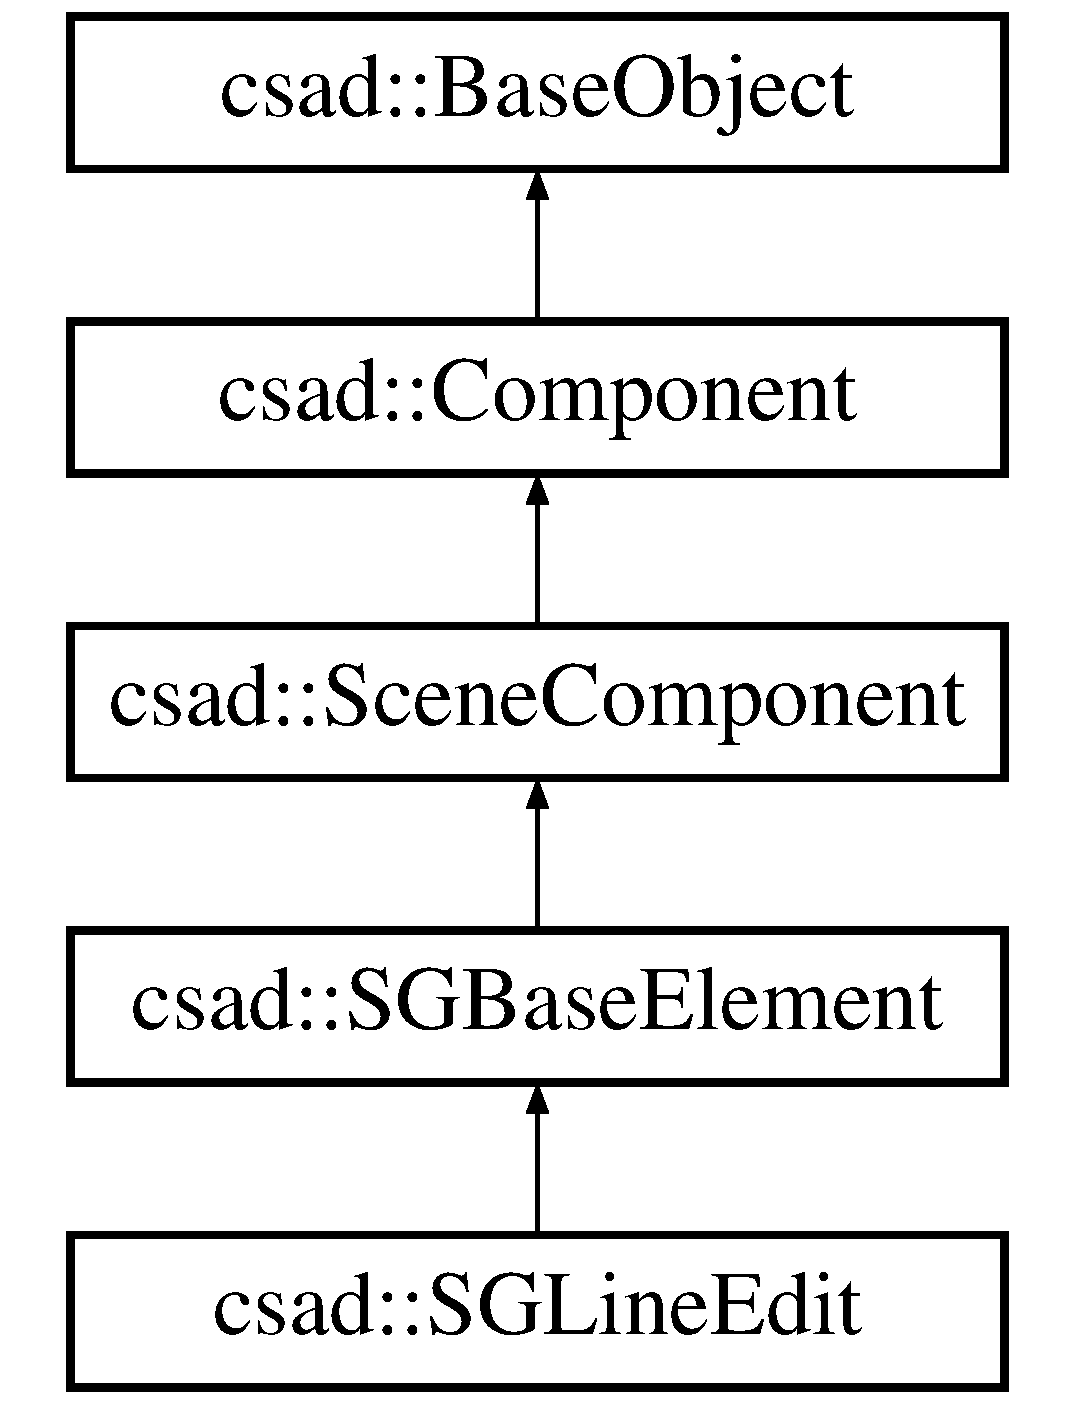
\includegraphics[height=5.000000cm]{classcsad_1_1_s_g_line_edit}
\end{center}
\end{figure}
\subsection*{Public Member Functions}
\begin{DoxyCompactItemize}
\item 
\hypertarget{classcsad_1_1_s_g_line_edit_a5a126be9c8b4af7538083362b0b58bdc}{C\-S\-A\-D\-\_\-\-A\-P\-I const char $\ast$ \hyperlink{classcsad_1_1_s_g_line_edit_a5a126be9c8b4af7538083362b0b58bdc}{get\-Text} ()}\label{classcsad_1_1_s_g_line_edit_a5a126be9c8b4af7538083362b0b58bdc}

\begin{DoxyCompactList}\small\item\em Возвращает текст (компоненты \hyperlink{classcsad_1_1_text3_d}{Text3\-D}) \end{DoxyCompactList}\item 
\hypertarget{classcsad_1_1_s_g_line_edit_a3cad93aa55612bc9d172465a8679d438}{\-\_\-\-F\-O\-R\-C\-E\-I\-N\-L\-I\-N\-E bool \hyperlink{classcsad_1_1_s_g_line_edit_a3cad93aa55612bc9d172465a8679d438}{is\-Click} ()}\label{classcsad_1_1_s_g_line_edit_a3cad93aa55612bc9d172465a8679d438}

\begin{DoxyCompactList}\small\item\em Returns true if set status Click. \end{DoxyCompactList}\item 
\hypertarget{classcsad_1_1_s_g_line_edit_a2c05a328fa166bdceacd46373993b185}{C\-S\-A\-D\-\_\-\-A\-P\-I void $\ast$ \hyperlink{classcsad_1_1_s_g_line_edit_a2c05a328fa166bdceacd46373993b185}{set} (unsigned \-\_\-int32, void $\ast$)}\label{classcsad_1_1_s_g_line_edit_a2c05a328fa166bdceacd46373993b185}

\begin{DoxyCompactList}\small\item\em used for any interface commands. \end{DoxyCompactList}\item 
\hypertarget{classcsad_1_1_s_g_line_edit_af31c5cc0e43a2822c1c7d14acbea3e51}{C\-S\-A\-D\-\_\-\-A\-P\-I void \hyperlink{classcsad_1_1_s_g_line_edit_af31c5cc0e43a2822c1c7d14acbea3e51}{set\-Set} (bool val)}\label{classcsad_1_1_s_g_line_edit_af31c5cc0e43a2822c1c7d14acbea3e51}

\begin{DoxyCompactList}\small\item\em Задает состояние активности редактирования. \end{DoxyCompactList}\item 
\hypertarget{classcsad_1_1_s_g_line_edit_a0e1e5c352a91c39448727727fe3a9b33}{C\-S\-A\-D\-\_\-\-A\-P\-I void \hyperlink{classcsad_1_1_s_g_line_edit_a0e1e5c352a91c39448727727fe3a9b33}{set\-Size} (\hyperlink{classbt_1_1vector3f}{vector3f} \&size)}\label{classcsad_1_1_s_g_line_edit_a0e1e5c352a91c39448727727fe3a9b33}

\begin{DoxyCompactList}\small\item\em Задать размер поля ввода \end{DoxyCompactList}\item 
\hypertarget{classcsad_1_1_s_g_line_edit_ad5a6c56e6f23e61f2bedc407dd60e7dc}{C\-S\-A\-D\-\_\-\-A\-P\-I void \hyperlink{classcsad_1_1_s_g_line_edit_ad5a6c56e6f23e61f2bedc407dd60e7dc}{set\-Style} (char $\ast$name)}\label{classcsad_1_1_s_g_line_edit_ad5a6c56e6f23e61f2bedc407dd60e7dc}

\begin{DoxyCompactList}\small\item\em Задает стиль \end{DoxyCompactList}\item 
\hypertarget{classcsad_1_1_s_g_line_edit_a637c4873077d232ad97efdc4465d3496}{C\-S\-A\-D\-\_\-\-A\-P\-I void \hyperlink{classcsad_1_1_s_g_line_edit_a637c4873077d232ad97efdc4465d3496}{set\-Style} (\hyperlink{classcsad_1_1_style}{Style} $\ast$style)}\label{classcsad_1_1_s_g_line_edit_a637c4873077d232ad97efdc4465d3496}

\begin{DoxyCompactList}\small\item\em Задает стиль \end{DoxyCompactList}\item 
\hypertarget{classcsad_1_1_s_g_line_edit_a48164102640747bdf5eb008c6e770d48}{C\-S\-A\-D\-\_\-\-A\-P\-I void \hyperlink{classcsad_1_1_s_g_line_edit_a48164102640747bdf5eb008c6e770d48}{set\-Text} (char $\ast$text)}\label{classcsad_1_1_s_g_line_edit_a48164102640747bdf5eb008c6e770d48}

\begin{DoxyCompactList}\small\item\em Задать редактируемый текст \end{DoxyCompactList}\item 
\hypertarget{classcsad_1_1_s_g_line_edit_a86fe803a2cb2f41a06f88813a7ca1d79}{\-\_\-\-F\-O\-R\-C\-E\-I\-N\-L\-I\-N\-E void \hyperlink{classcsad_1_1_s_g_line_edit_a86fe803a2cb2f41a06f88813a7ca1d79}{set\-Text} (const char $\ast$text)}\label{classcsad_1_1_s_g_line_edit_a86fe803a2cb2f41a06f88813a7ca1d79}

\begin{DoxyCompactList}\small\item\em Задать редактируемый текст \end{DoxyCompactList}\item 
\hypertarget{classcsad_1_1_s_g_line_edit_a4e71eeb69a9f032d500e1560bf698b9f}{C\-S\-A\-D\-\_\-\-A\-P\-I void \hyperlink{classcsad_1_1_s_g_line_edit_a4e71eeb69a9f032d500e1560bf698b9f}{set\-Visible} (bool val)}\label{classcsad_1_1_s_g_line_edit_a4e71eeb69a9f032d500e1560bf698b9f}

\begin{DoxyCompactList}\small\item\em Задает состояние видимости \end{DoxyCompactList}\item 
\hypertarget{classcsad_1_1_s_g_line_edit_a9f9d2db8af333e47660e718cbce55c26}{C\-S\-A\-D\-\_\-\-A\-P\-I void \hyperlink{classcsad_1_1_s_g_line_edit_a9f9d2db8af333e47660e718cbce55c26}{start} ()}\label{classcsad_1_1_s_g_line_edit_a9f9d2db8af333e47660e718cbce55c26}

\begin{DoxyCompactList}\small\item\em This event is fired after the program start. \end{DoxyCompactList}\item 
\hypertarget{classcsad_1_1_s_g_line_edit_a1e200a29f617af3184350b90a20f67bf}{C\-S\-A\-D\-\_\-\-A\-P\-I void \hyperlink{classcsad_1_1_s_g_line_edit_a1e200a29f617af3184350b90a20f67bf}{update} ()}\label{classcsad_1_1_s_g_line_edit_a1e200a29f617af3184350b90a20f67bf}

\begin{DoxyCompactList}\small\item\em This event is fired before rendering environment container component. \end{DoxyCompactList}\end{DoxyCompactItemize}
\subsection*{Additional Inherited Members}


\subsection{Detailed Description}
\hyperlink{classcsad_1_1_s_g_line_edit}{S\-G\-Line\-Edit} -\/ component. 

For description in the configuration\-: \begin{DoxyVerb}  <Transform name="the name of the scene">
      <SGLineEdit size="0.3 0.1 0.0" text="test text"/>
  </Transform>
\end{DoxyVerb}


\begin{DoxySeeAlso}{See Also}
\hyperlink{classcsad_1_1_transform}{Transform}, \hyperlink{classcsad_1_1_s_g_line_edit_style}{S\-G\-Line\-Edit\-Style}, \hyperlink{classcsad_1_1_s_g_base_element}{S\-G\-Base\-Element}, \hyperlink{group__scenegui}{csad\-: gui} 
\end{DoxySeeAlso}

\hypertarget{classcsad_1_1_s_g_line_edit_style}{\section{csad\-:\-:S\-G\-Line\-Edit\-Style Class Reference}
\label{classcsad_1_1_s_g_line_edit_style}\index{csad\-::\-S\-G\-Line\-Edit\-Style@{csad\-::\-S\-G\-Line\-Edit\-Style}}
}


\hyperlink{classcsad_1_1_s_g_line_edit_style}{S\-G\-Line\-Edit\-Style} -\/ component containing the parameters of the line edit state.  




Inherits csad\-::\-S\-G\-Style.

\subsection*{Public Member Functions}
\begin{DoxyCompactItemize}
\item 
\hypertarget{classcsad_1_1_s_g_line_edit_style_a0e6084eeae9c28da54c1d04f3c56e04e}{C\-S\-A\-D\-\_\-\-A\-P\-I void $\ast$ \hyperlink{classcsad_1_1_s_g_line_edit_style_a0e6084eeae9c28da54c1d04f3c56e04e}{set} (unsigned \-\_\-int32, void $\ast$)}\label{classcsad_1_1_s_g_line_edit_style_a0e6084eeae9c28da54c1d04f3c56e04e}

\begin{DoxyCompactList}\small\item\em used for any interface commands. \end{DoxyCompactList}\end{DoxyCompactItemize}
\subsection*{Additional Inherited Members}


\subsection{Detailed Description}
\hyperlink{classcsad_1_1_s_g_line_edit_style}{S\-G\-Line\-Edit\-Style} -\/ component containing the parameters of the line edit state. 

\begin{DoxySeeAlso}{See Also}
\hyperlink{group__scenegui}{csad\-: gui}, \hyperlink{classcsad_1_1_s_g_line_edit}{S\-G\-Line\-Edit} 
\end{DoxySeeAlso}

\hypertarget{classcsad_1_1_s_g_mouse}{\section{csad\-:\-:S\-G\-Mouse Class Reference}
\label{classcsad_1_1_s_g_mouse}\index{csad\-::\-S\-G\-Mouse@{csad\-::\-S\-G\-Mouse}}
}


\hyperlink{classcsad_1_1_s_g_mouse}{S\-G\-Mouse} -\/ component, mouse event handlers.  


Inheritance diagram for csad\-:\-:S\-G\-Mouse\-:\begin{figure}[H]
\begin{center}
\leavevmode
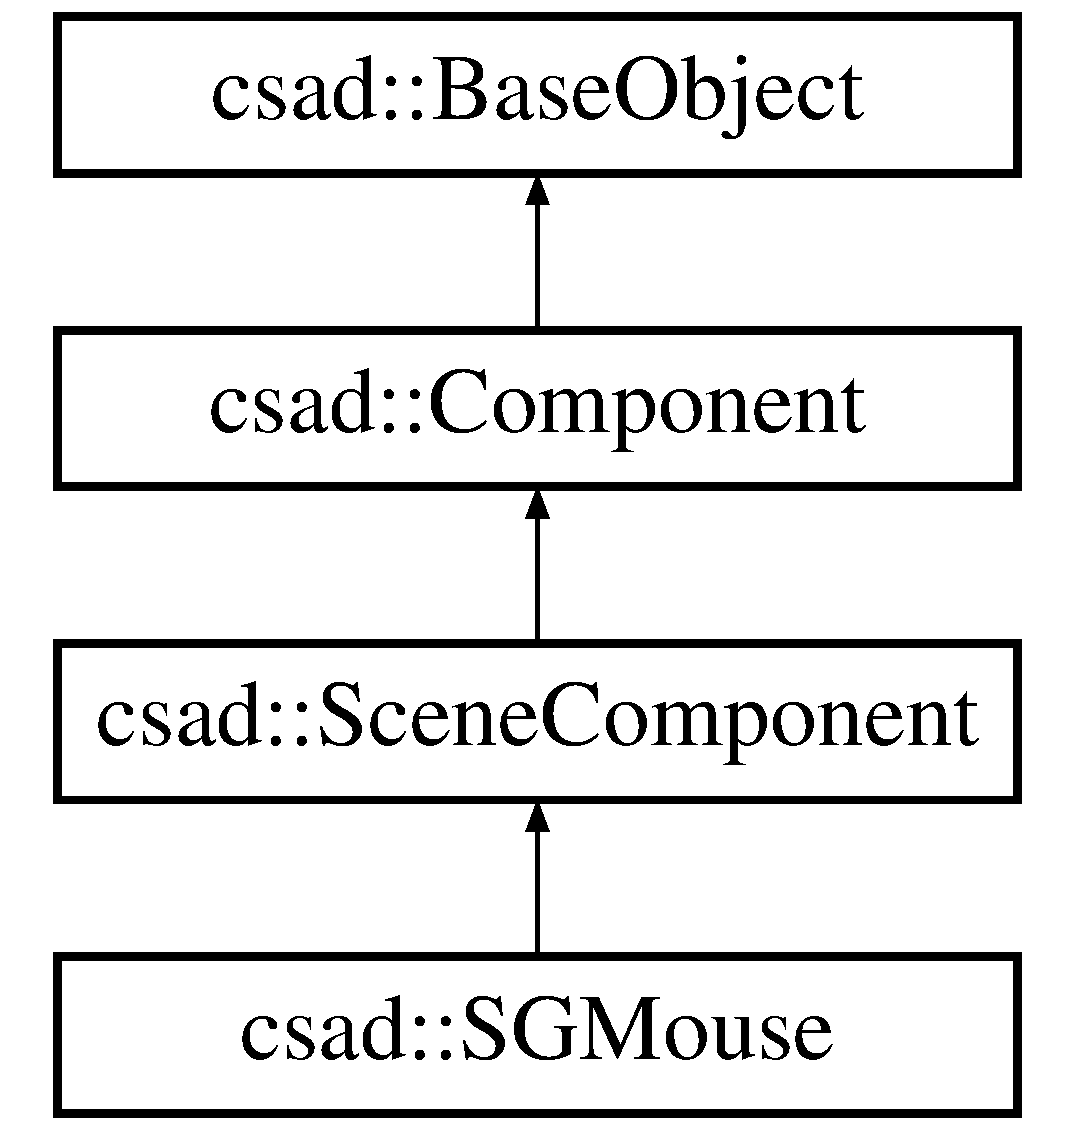
\includegraphics[height=4.000000cm]{classcsad_1_1_s_g_mouse}
\end{center}
\end{figure}
\subsection*{Public Member Functions}
\begin{DoxyCompactItemize}
\item 
\hypertarget{classcsad_1_1_s_g_mouse_a35dc2a65e9f0457a9983a85fa3a9cb88}{C\-S\-A\-D\-\_\-\-A\-P\-I void \hyperlink{classcsad_1_1_s_g_mouse_a35dc2a65e9f0457a9983a85fa3a9cb88}{prepare} ()}\label{classcsad_1_1_s_g_mouse_a35dc2a65e9f0457a9983a85fa3a9cb88}

\begin{DoxyCompactList}\small\item\em The event is called during the preparation stage. \end{DoxyCompactList}\item 
\hypertarget{classcsad_1_1_s_g_mouse_a65eebbd5eb437c2d93c0dcc1aae3f167}{C\-S\-A\-D\-\_\-\-A\-P\-I void $\ast$ \hyperlink{classcsad_1_1_s_g_mouse_a65eebbd5eb437c2d93c0dcc1aae3f167}{set} (unsigned \-\_\-int32, void $\ast$)}\label{classcsad_1_1_s_g_mouse_a65eebbd5eb437c2d93c0dcc1aae3f167}

\begin{DoxyCompactList}\small\item\em used for any interface commands. \end{DoxyCompactList}\item 
C\-S\-A\-D\-\_\-\-A\-P\-I void \hyperlink{classcsad_1_1_s_g_mouse_ae759f467750f0a48749da3ec2d037269}{set\-Zoom} (float scale)
\end{DoxyCompactItemize}
\subsection*{Additional Inherited Members}


\subsection{Detailed Description}
\hyperlink{classcsad_1_1_s_g_mouse}{S\-G\-Mouse} -\/ component, mouse event handlers. 

For description in the configuration\-: \begin{DoxyVerb}  <Scene name="myMouseScene">
    <Transform>
      <SGMouse speed="1"/>
    </Transform>
  </Scene>
\end{DoxyVerb}


\begin{DoxySeeAlso}{See Also}
\hyperlink{group__scenegui}{csad\-: gui}, \hyperlink{classcsad_1_1_s_g_mouse_mesh}{S\-G\-Mouse\-Mesh}, \hyperlink{classcsad_1_1_style}{Style}, \hyperlink{classcsad_1_1_text_style}{Text\-Style}, \hyperlink{classcsad_1_1_s_g_button_style}{S\-G\-Button\-Style}, \hyperlink{classcsad_1_1_base_object}{Base\-Object} 
\end{DoxySeeAlso}


\subsection{Member Function Documentation}
\hypertarget{classcsad_1_1_s_g_mouse_ae759f467750f0a48749da3ec2d037269}{\index{csad\-::\-S\-G\-Mouse@{csad\-::\-S\-G\-Mouse}!set\-Zoom@{set\-Zoom}}
\index{set\-Zoom@{set\-Zoom}!csad::SGMouse@{csad\-::\-S\-G\-Mouse}}
\subsubsection[{set\-Zoom}]{\setlength{\rightskip}{0pt plus 5cm}C\-S\-A\-D\-\_\-\-A\-P\-I void csad\-::\-S\-G\-Mouse\-::set\-Zoom (
\begin{DoxyParamCaption}
\item[{float}]{scale}
\end{DoxyParamCaption}
)}}\label{classcsad_1_1_s_g_mouse_ae759f467750f0a48749da3ec2d037269}
Sets the zoom speed. For the orthogonal projection size camera 1.\-0, direct correspondence screen coordinates speed reverse the height of the screen in pixels. 
\hypertarget{classcsad_1_1_s_g_mouse_mesh}{\section{csad\-:\-:S\-G\-Mouse\-Mesh Class Reference}
\label{classcsad_1_1_s_g_mouse_mesh}\index{csad\-::\-S\-G\-Mouse\-Mesh@{csad\-::\-S\-G\-Mouse\-Mesh}}
}


\hyperlink{classcsad_1_1_s_g_mouse_mesh}{S\-G\-Mouse\-Mesh} -\/ component, geometrical model of the pointer.  


Inheritance diagram for csad\-:\-:S\-G\-Mouse\-Mesh\-:\begin{figure}[H]
\begin{center}
\leavevmode
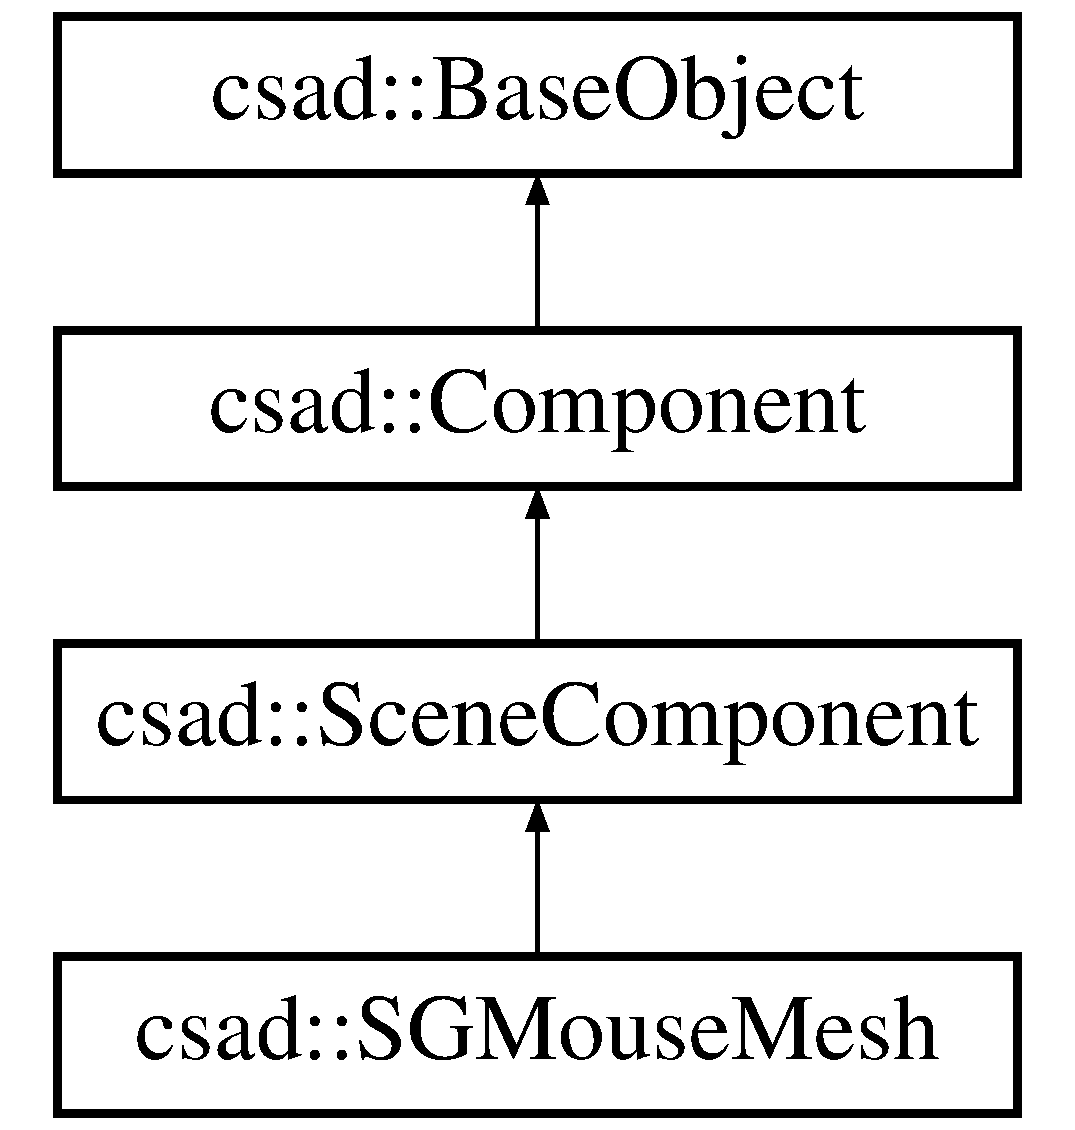
\includegraphics[height=4.000000cm]{classcsad_1_1_s_g_mouse_mesh}
\end{center}
\end{figure}
\subsection*{Public Member Functions}
\begin{DoxyCompactItemize}
\item 
\hypertarget{classcsad_1_1_s_g_mouse_mesh_a6dbc5eaeb35808a682bd713fdbc0af9e}{C\-S\-A\-D\-\_\-\-A\-P\-I void \hyperlink{classcsad_1_1_s_g_mouse_mesh_a6dbc5eaeb35808a682bd713fdbc0af9e}{prepare} ()}\label{classcsad_1_1_s_g_mouse_mesh_a6dbc5eaeb35808a682bd713fdbc0af9e}

\begin{DoxyCompactList}\small\item\em The event is called during the preparation stage. \end{DoxyCompactList}\item 
\hypertarget{classcsad_1_1_s_g_mouse_mesh_a778567be046067f8afbabfbe43ac0449}{C\-S\-A\-D\-\_\-\-A\-P\-I void \hyperlink{classcsad_1_1_s_g_mouse_mesh_a778567be046067f8afbabfbe43ac0449}{quit} ()}\label{classcsad_1_1_s_g_mouse_mesh_a778567be046067f8afbabfbe43ac0449}

\begin{DoxyCompactList}\small\item\em The event is called before the program exits. \end{DoxyCompactList}\item 
\hypertarget{classcsad_1_1_s_g_mouse_mesh_a2ef2490d6609a4ea87bffca4de6a0476}{C\-S\-A\-D\-\_\-\-A\-P\-I void $\ast$ \hyperlink{classcsad_1_1_s_g_mouse_mesh_a2ef2490d6609a4ea87bffca4de6a0476}{set} (unsigned \-\_\-int32, void $\ast$)}\label{classcsad_1_1_s_g_mouse_mesh_a2ef2490d6609a4ea87bffca4de6a0476}

\begin{DoxyCompactList}\small\item\em used for any interface commands. \end{DoxyCompactList}\item 
\hypertarget{classcsad_1_1_s_g_mouse_mesh_a623caa5aac16b3d846b2d39a426d002a}{C\-S\-A\-D\-\_\-\-A\-P\-I void \hyperlink{classcsad_1_1_s_g_mouse_mesh_a623caa5aac16b3d846b2d39a426d002a}{set\-Line\-Material} (char $\ast$name)}\label{classcsad_1_1_s_g_mouse_mesh_a623caa5aac16b3d846b2d39a426d002a}

\begin{DoxyCompactList}\small\item\em Setting material for mouse line geometry. \end{DoxyCompactList}\item 
\hypertarget{classcsad_1_1_s_g_mouse_mesh_a3646d0f79c4f4999a1fd17f0285adbba}{C\-S\-A\-D\-\_\-\-A\-P\-I void \hyperlink{classcsad_1_1_s_g_mouse_mesh_a3646d0f79c4f4999a1fd17f0285adbba}{set\-Material} (char $\ast$name)}\label{classcsad_1_1_s_g_mouse_mesh_a3646d0f79c4f4999a1fd17f0285adbba}

\begin{DoxyCompactList}\small\item\em Setting material for mouse geometry. \end{DoxyCompactList}\item 
\hypertarget{classcsad_1_1_s_g_mouse_mesh_afe05b3cbdc3e2485c1d91e3c00c59f4a}{C\-S\-A\-D\-\_\-\-A\-P\-I void \hyperlink{classcsad_1_1_s_g_mouse_mesh_afe05b3cbdc3e2485c1d91e3c00c59f4a}{start} ()}\label{classcsad_1_1_s_g_mouse_mesh_afe05b3cbdc3e2485c1d91e3c00c59f4a}

\begin{DoxyCompactList}\small\item\em This event is fired after the program start. \end{DoxyCompactList}\end{DoxyCompactItemize}
\subsection*{Additional Inherited Members}


\subsection{Detailed Description}
\hyperlink{classcsad_1_1_s_g_mouse_mesh}{S\-G\-Mouse\-Mesh} -\/ component, geometrical model of the pointer. 

For description in the configuration\-: \begin{DoxyVerb}  <Scene name="myMouseScene">
    <Transform>
      <SGMouse speed="1"/>
      <SGMouseMesh material="" linematerial=""/>
    </Transform>
  </Scene>
\end{DoxyVerb}


\begin{DoxySeeAlso}{See Also}
\hyperlink{group__scenegui}{csad\-: gui}, \hyperlink{classcsad_1_1_s_g_mouse}{S\-G\-Mouse}, \hyperlink{classcsad_1_1_style}{Style}, \hyperlink{classcsad_1_1_text_style}{Text\-Style}, \hyperlink{classcsad_1_1_s_g_button_style}{S\-G\-Button\-Style}, \hyperlink{classcsad_1_1_base_object}{Base\-Object} 
\end{DoxySeeAlso}

\hypertarget{classcsad_1_1_s_g_scroll}{\section{csad\-:\-:S\-G\-Scroll Class Reference}
\label{classcsad_1_1_s_g_scroll}\index{csad\-::\-S\-G\-Scroll@{csad\-::\-S\-G\-Scroll}}
}


\hyperlink{classcsad_1_1_s_g_scroll}{S\-G\-Scroll} -\/ component, which is the controller of the scrolls, defines the characteristics of the image and manages events.  


Inheritance diagram for csad\-:\-:S\-G\-Scroll\-:\begin{figure}[H]
\begin{center}
\leavevmode
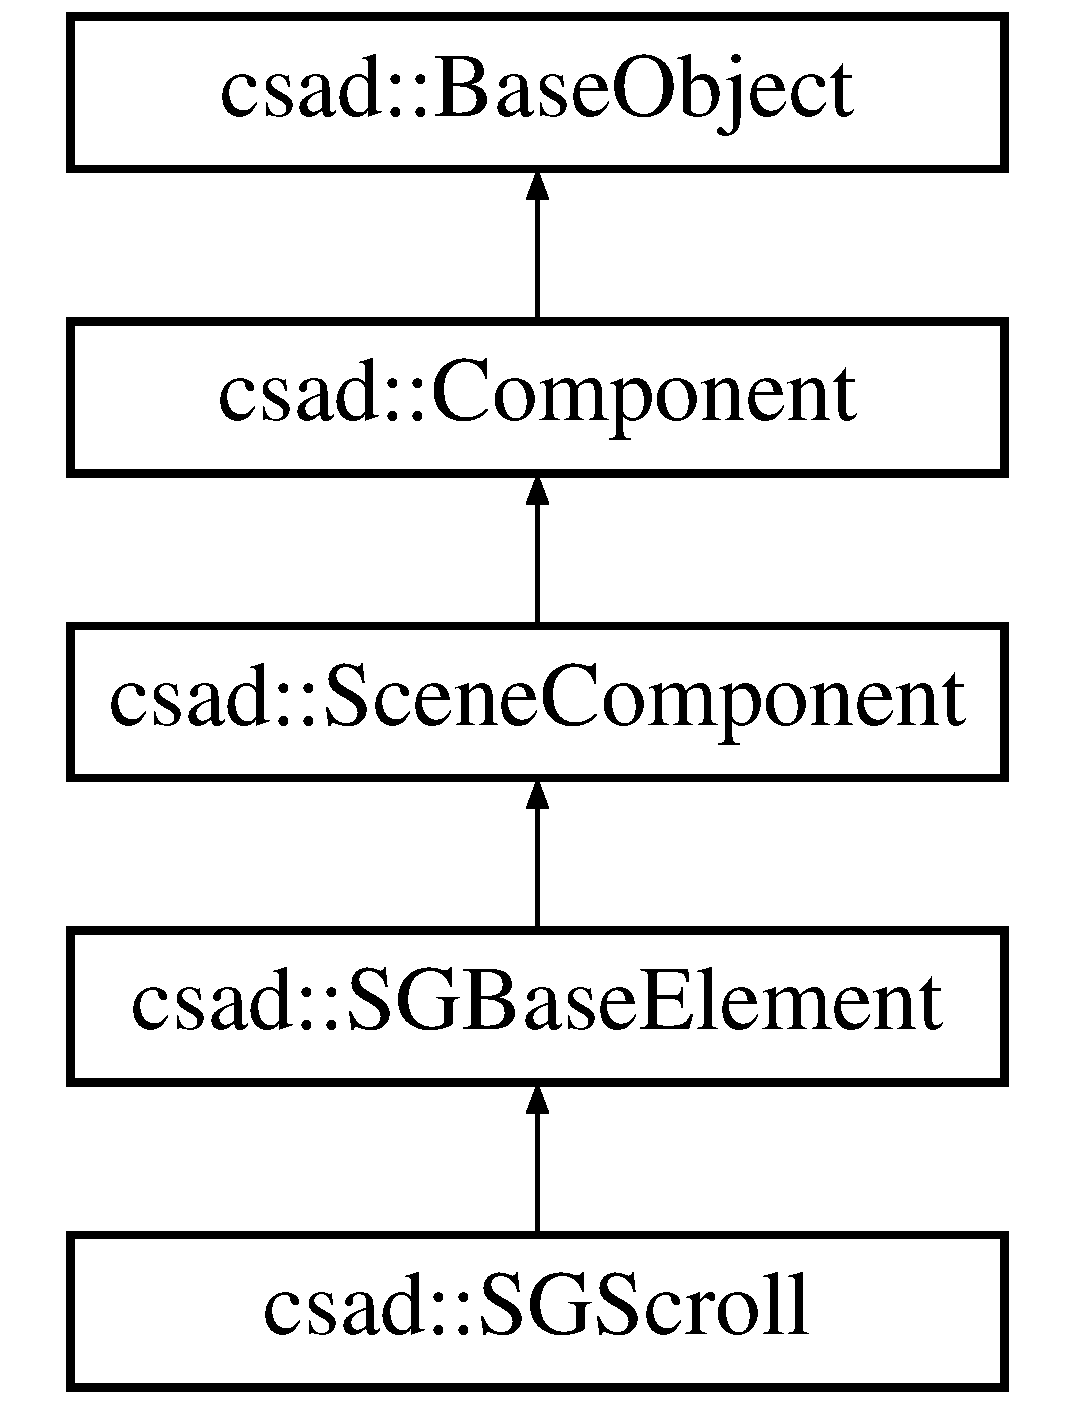
\includegraphics[height=5.000000cm]{classcsad_1_1_s_g_scroll}
\end{center}
\end{figure}
\subsection*{Public Member Functions}
\begin{DoxyCompactItemize}
\item 
\hypertarget{classcsad_1_1_s_g_scroll_ace749f35d40557d46889cee3114d57d0}{C\-S\-A\-D\-\_\-\-A\-P\-I void \hyperlink{classcsad_1_1_s_g_scroll_ace749f35d40557d46889cee3114d57d0}{prepare} ()}\label{classcsad_1_1_s_g_scroll_ace749f35d40557d46889cee3114d57d0}

\begin{DoxyCompactList}\small\item\em The event is called during the preparation stage. \end{DoxyCompactList}\item 
\hypertarget{classcsad_1_1_s_g_scroll_a7205cce98300f63dbf3f4fdf0ee9b38e}{C\-S\-A\-D\-\_\-\-A\-P\-I void $\ast$ \hyperlink{classcsad_1_1_s_g_scroll_a7205cce98300f63dbf3f4fdf0ee9b38e}{set} (unsigned \-\_\-int32, void $\ast$)}\label{classcsad_1_1_s_g_scroll_a7205cce98300f63dbf3f4fdf0ee9b38e}

\begin{DoxyCompactList}\small\item\em used for any interface commands. \end{DoxyCompactList}\item 
C\-S\-A\-D\-\_\-\-A\-P\-I void \hyperlink{classcsad_1_1_s_g_scroll_a5fb534de72e2730233871692f88e9e95}{set\-Receiver} (char $\ast$path)
\item 
C\-S\-A\-D\-\_\-\-A\-P\-I void \hyperlink{classcsad_1_1_s_g_scroll_a0e6130ea34137b0c3a5642808b080942}{set\-Receiver} (\hyperlink{classcsad_1_1_base_object}{Base\-Object} $\ast$obj)
\item 
\hypertarget{classcsad_1_1_s_g_scroll_aa2d6ef27b51ae6450eeb04fafd13b608}{C\-S\-A\-D\-\_\-\-A\-P\-I \hyperlink{classcsad_1_1_s_g_scroll}{S\-G\-Scroll} \& \hyperlink{classcsad_1_1_s_g_scroll_aa2d6ef27b51ae6450eeb04fafd13b608}{set\-Size} (\hyperlink{classbt_1_1vector3f}{vector3f} \&size)}\label{classcsad_1_1_s_g_scroll_aa2d6ef27b51ae6450eeb04fafd13b608}

\begin{DoxyCompactList}\small\item\em Задает размер полосы \end{DoxyCompactList}\item 
\hypertarget{classcsad_1_1_s_g_scroll_a44a79019f584b84eeca4165a33b8272d}{C\-S\-A\-D\-\_\-\-A\-P\-I void \hyperlink{classcsad_1_1_s_g_scroll_a44a79019f584b84eeca4165a33b8272d}{set\-Style} (char $\ast$name)}\label{classcsad_1_1_s_g_scroll_a44a79019f584b84eeca4165a33b8272d}

\begin{DoxyCompactList}\small\item\em Sets the style named. \end{DoxyCompactList}\item 
\hypertarget{classcsad_1_1_s_g_scroll_adde70cbc4a41c13a6e9abf6ea02aa786}{C\-S\-A\-D\-\_\-\-A\-P\-I void \hyperlink{classcsad_1_1_s_g_scroll_adde70cbc4a41c13a6e9abf6ea02aa786}{set\-Style} (\hyperlink{classcsad_1_1_style}{Style} $\ast$style)}\label{classcsad_1_1_s_g_scroll_adde70cbc4a41c13a6e9abf6ea02aa786}

\begin{DoxyCompactList}\small\item\em Задает объект стиля \end{DoxyCompactList}\item 
\hypertarget{classcsad_1_1_s_g_scroll_a0ac81135777ee1f12b92df6fa82133c9}{C\-S\-A\-D\-\_\-\-A\-P\-I void \hyperlink{classcsad_1_1_s_g_scroll_a0ac81135777ee1f12b92df6fa82133c9}{start} ()}\label{classcsad_1_1_s_g_scroll_a0ac81135777ee1f12b92df6fa82133c9}

\begin{DoxyCompactList}\small\item\em This event is fired after the program start. \end{DoxyCompactList}\item 
\hypertarget{classcsad_1_1_s_g_scroll_aad3aeb52dc14de4116fc9f855723c97f}{C\-S\-A\-D\-\_\-\-A\-P\-I void \hyperlink{classcsad_1_1_s_g_scroll_aad3aeb52dc14de4116fc9f855723c97f}{update} ()}\label{classcsad_1_1_s_g_scroll_aad3aeb52dc14de4116fc9f855723c97f}

\begin{DoxyCompactList}\small\item\em This event is fired before rendering environment container component. \end{DoxyCompactList}\end{DoxyCompactItemize}
\subsection*{Additional Inherited Members}


\subsection{Detailed Description}
\hyperlink{classcsad_1_1_s_g_scroll}{S\-G\-Scroll} -\/ component, which is the controller of the scrolls, defines the characteristics of the image and manages events. 

\begin{DoxySeeAlso}{See Also}
\hyperlink{group__scenegui}{csad\-: gui} 
\end{DoxySeeAlso}


\subsection{Member Function Documentation}
\hypertarget{classcsad_1_1_s_g_scroll_a5fb534de72e2730233871692f88e9e95}{\index{csad\-::\-S\-G\-Scroll@{csad\-::\-S\-G\-Scroll}!set\-Receiver@{set\-Receiver}}
\index{set\-Receiver@{set\-Receiver}!csad::SGScroll@{csad\-::\-S\-G\-Scroll}}
\subsubsection[{set\-Receiver}]{\setlength{\rightskip}{0pt plus 5cm}C\-S\-A\-D\-\_\-\-A\-P\-I void csad\-::\-S\-G\-Scroll\-::set\-Receiver (
\begin{DoxyParamCaption}
\item[{char $\ast$}]{path}
\end{DoxyParamCaption}
)}}\label{classcsad_1_1_s_g_scroll_a5fb534de72e2730233871692f88e9e95}
Задает получателя событий по его пути \begin{DoxySeeAlso}{See Also}
\hyperlink{classcsad_1_1_base_object_a27d9db492c1a385aa4086da1824e2737a1ad754d1312e455b8585419a33bba1bf}{Base\-Object\-::\-S\-E\-L\-E\-C\-T} 
\end{DoxySeeAlso}
\hypertarget{classcsad_1_1_s_g_scroll_a0e6130ea34137b0c3a5642808b080942}{\index{csad\-::\-S\-G\-Scroll@{csad\-::\-S\-G\-Scroll}!set\-Receiver@{set\-Receiver}}
\index{set\-Receiver@{set\-Receiver}!csad::SGScroll@{csad\-::\-S\-G\-Scroll}}
\subsubsection[{set\-Receiver}]{\setlength{\rightskip}{0pt plus 5cm}C\-S\-A\-D\-\_\-\-A\-P\-I void csad\-::\-S\-G\-Scroll\-::set\-Receiver (
\begin{DoxyParamCaption}
\item[{{\bf Base\-Object} $\ast$}]{obj}
\end{DoxyParamCaption}
)}}\label{classcsad_1_1_s_g_scroll_a0e6130ea34137b0c3a5642808b080942}
Задает объект получателя \begin{DoxySeeAlso}{See Also}
\hyperlink{classcsad_1_1_base_object_a27d9db492c1a385aa4086da1824e2737a1ad754d1312e455b8585419a33bba1bf}{Base\-Object\-::\-S\-E\-L\-E\-C\-T} 
\end{DoxySeeAlso}

\hypertarget{classcsad_1_1_s_g_tab_controll}{\section{csad\-:\-:S\-G\-Tab\-Controll Class Reference}
\label{classcsad_1_1_s_g_tab_controll}\index{csad\-::\-S\-G\-Tab\-Controll@{csad\-::\-S\-G\-Tab\-Controll}}
}


\hyperlink{classcsad_1_1_s_g_tab_controll}{S\-G\-Tab\-Controll} -\/ .  


Inheritance diagram for csad\-:\-:S\-G\-Tab\-Controll\-:\begin{figure}[H]
\begin{center}
\leavevmode
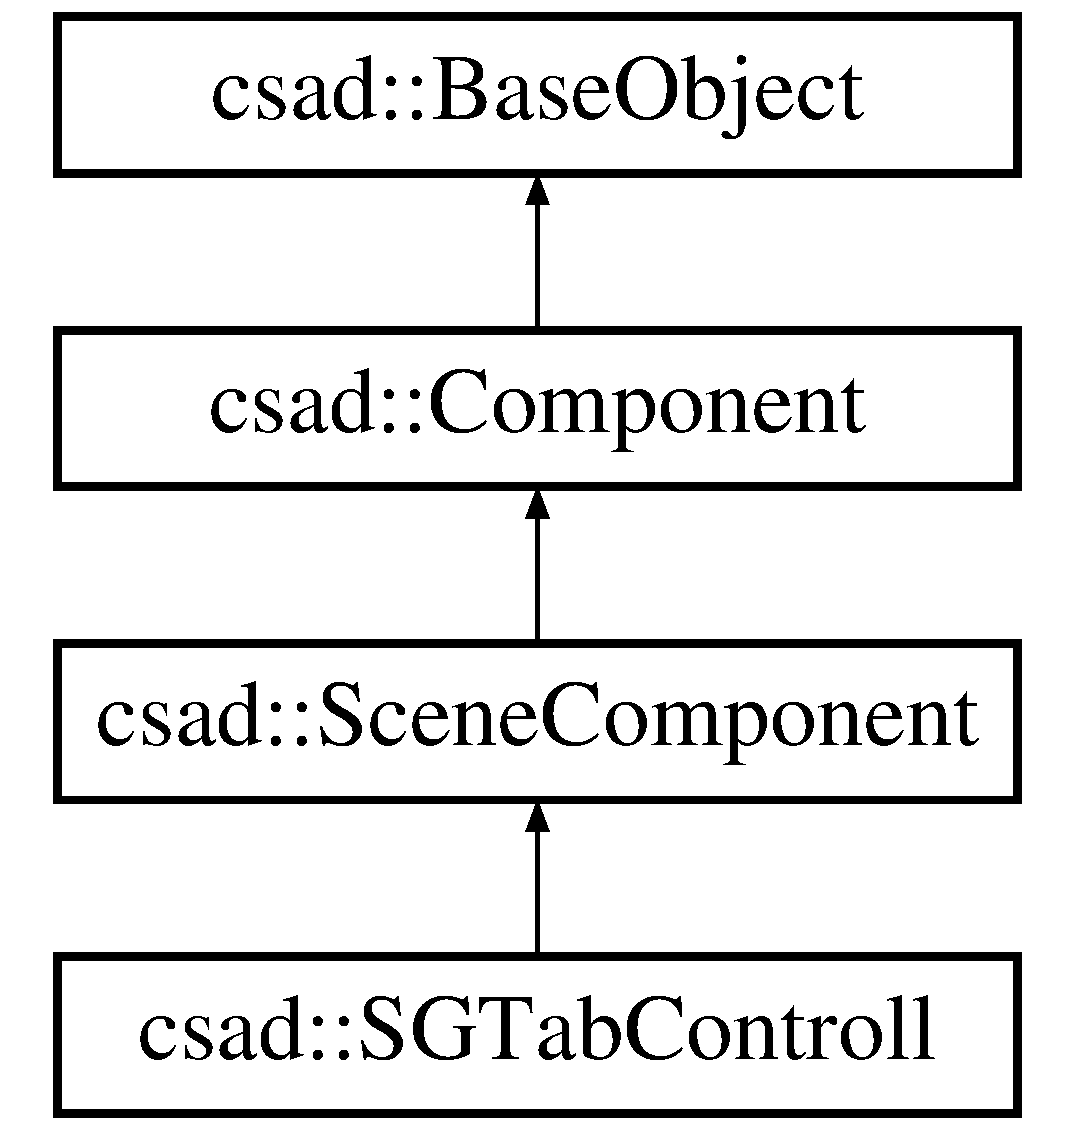
\includegraphics[height=4.000000cm]{classcsad_1_1_s_g_tab_controll}
\end{center}
\end{figure}
\subsection*{Public Member Functions}
\begin{DoxyCompactItemize}
\item 
\hypertarget{classcsad_1_1_s_g_tab_controll_ae535ab52a7000f97913e31b0af7a5a41}{C\-S\-A\-D\-\_\-\-A\-P\-I void $\ast$ \hyperlink{classcsad_1_1_s_g_tab_controll_ae535ab52a7000f97913e31b0af7a5a41}{set} (unsigned \-\_\-int32, void $\ast$)}\label{classcsad_1_1_s_g_tab_controll_ae535ab52a7000f97913e31b0af7a5a41}

\begin{DoxyCompactList}\small\item\em used for any interface commands. \end{DoxyCompactList}\end{DoxyCompactItemize}
\subsection*{Additional Inherited Members}


\subsection{Detailed Description}
\hyperlink{classcsad_1_1_s_g_tab_controll}{S\-G\-Tab\-Controll} -\/ . 

For description in the configuration\-: \begin{DoxyVerb}  <Transform name="TabList">
     <SGTabControll keys="TabKeys"/>
  </Transform>
\end{DoxyVerb}


\begin{DoxySeeAlso}{See Also}
\hyperlink{group__scenegui}{csad\-: gui}, \hyperlink{classcsad_1_1_s_g_button}{S\-G\-Button} 
\end{DoxySeeAlso}

\hypertarget{classcsad_1_1_s_g_table}{\section{csad\-:\-:S\-G\-Table Class Reference}
\label{classcsad_1_1_s_g_table}\index{csad\-::\-S\-G\-Table@{csad\-::\-S\-G\-Table}}
}


\hyperlink{classcsad_1_1_s_g_table}{S\-G\-Table} -\/ component.  


Inheritance diagram for csad\-:\-:S\-G\-Table\-:\begin{figure}[H]
\begin{center}
\leavevmode
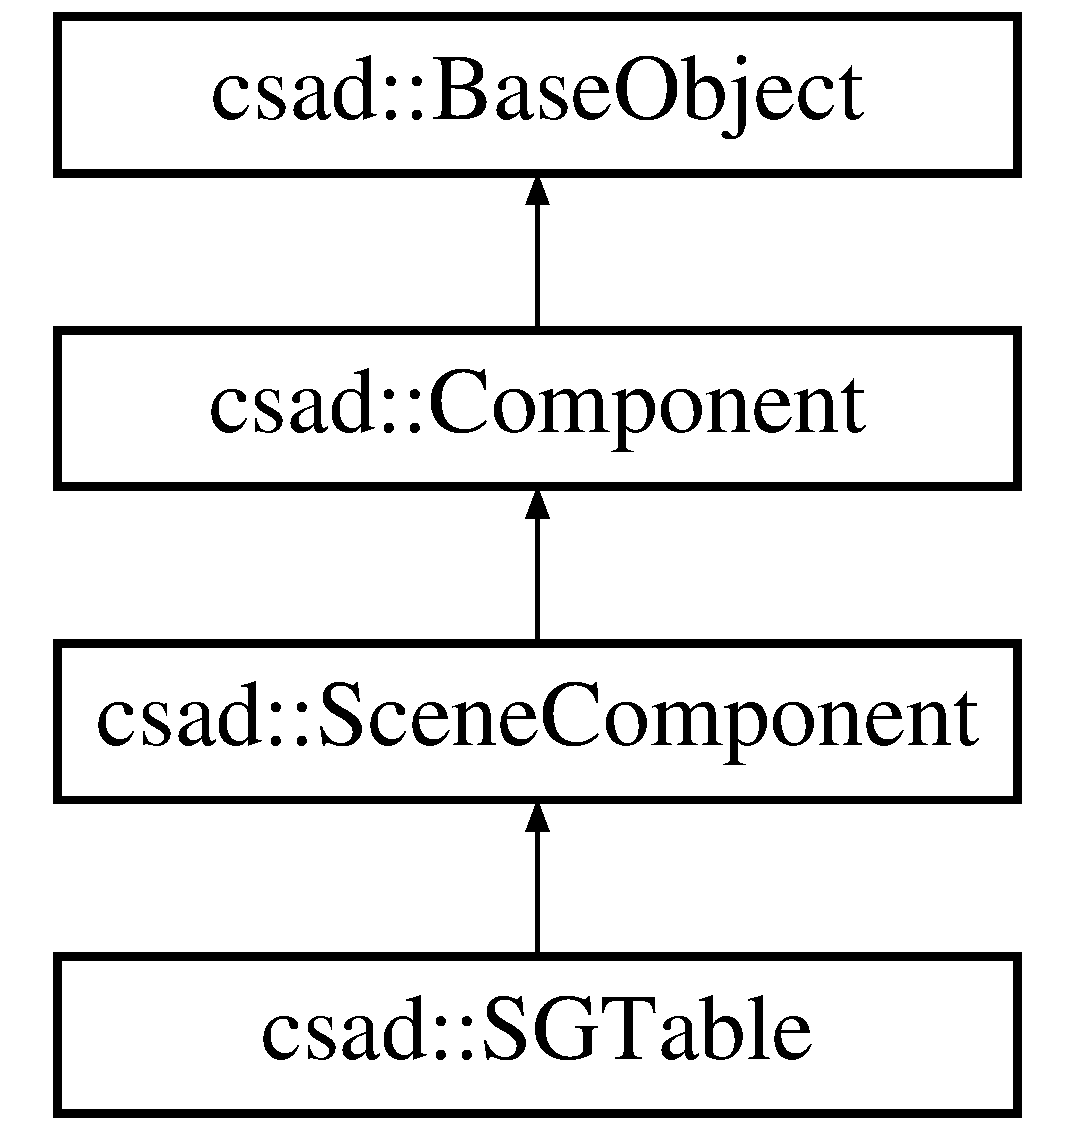
\includegraphics[height=4.000000cm]{classcsad_1_1_s_g_table}
\end{center}
\end{figure}
\subsection*{Public Member Functions}
\begin{DoxyCompactItemize}
\item 
\hypertarget{classcsad_1_1_s_g_table_a75eab0af569c25ac1a1ad1b24a41ac75}{C\-S\-A\-D\-\_\-\-A\-P\-I void $\ast$ \hyperlink{classcsad_1_1_s_g_table_a75eab0af569c25ac1a1ad1b24a41ac75}{set} (unsigned \-\_\-int32, void $\ast$)}\label{classcsad_1_1_s_g_table_a75eab0af569c25ac1a1ad1b24a41ac75}

\begin{DoxyCompactList}\small\item\em used for any interface commands. \end{DoxyCompactList}\item 
\hypertarget{classcsad_1_1_s_g_table_a64ec6a06f51d8b7d05bab1d40a441512}{C\-S\-A\-D\-\_\-\-A\-P\-I void \hyperlink{classcsad_1_1_s_g_table_a64ec6a06f51d8b7d05bab1d40a441512}{set\-Style} (char $\ast$name)}\label{classcsad_1_1_s_g_table_a64ec6a06f51d8b7d05bab1d40a441512}

\begin{DoxyCompactList}\small\item\em Задать редактируемый текст \end{DoxyCompactList}\item 
\hypertarget{classcsad_1_1_s_g_table_ae126133833123f83a508d75e176aa048}{C\-S\-A\-D\-\_\-\-A\-P\-I void \hyperlink{classcsad_1_1_s_g_table_ae126133833123f83a508d75e176aa048}{start} ()}\label{classcsad_1_1_s_g_table_ae126133833123f83a508d75e176aa048}

\begin{DoxyCompactList}\small\item\em This event is fired after the program start. \end{DoxyCompactList}\item 
\hypertarget{classcsad_1_1_s_g_table_a638deff0606055500ce94fde9bfe5351}{C\-S\-A\-D\-\_\-\-A\-P\-I void \hyperlink{classcsad_1_1_s_g_table_a638deff0606055500ce94fde9bfe5351}{update} ()}\label{classcsad_1_1_s_g_table_a638deff0606055500ce94fde9bfe5351}

\begin{DoxyCompactList}\small\item\em This event is fired before rendering environment container component. \end{DoxyCompactList}\end{DoxyCompactItemize}
\subsection*{Additional Inherited Members}


\subsection{Detailed Description}
\hyperlink{classcsad_1_1_s_g_table}{S\-G\-Table} -\/ component. 

For description in the configuration\-: \begin{DoxyVerb}  <Transform name="the name of the scene">
      <SGTable size="0.3 0.1 0.0" columns="3" records="10"/>
  </Transform>
\end{DoxyVerb}


\begin{DoxySeeAlso}{See Also}
\hyperlink{classcsad_1_1_s_g_base_element}{S\-G\-Base\-Element}, \hyperlink{group__scenegui}{csad\-: gui} 
\end{DoxySeeAlso}

\hypertarget{classcsad_1_1_shader}{\section{csad\-:\-:Shader Class Reference}
\label{classcsad_1_1_shader}\index{csad\-::\-Shader@{csad\-::\-Shader}}
}


\hyperlink{classcsad_1_1_shader}{Shader} -\/ the object of shader programm.  


Inheritance diagram for csad\-:\-:Shader\-:\begin{figure}[H]
\begin{center}
\leavevmode
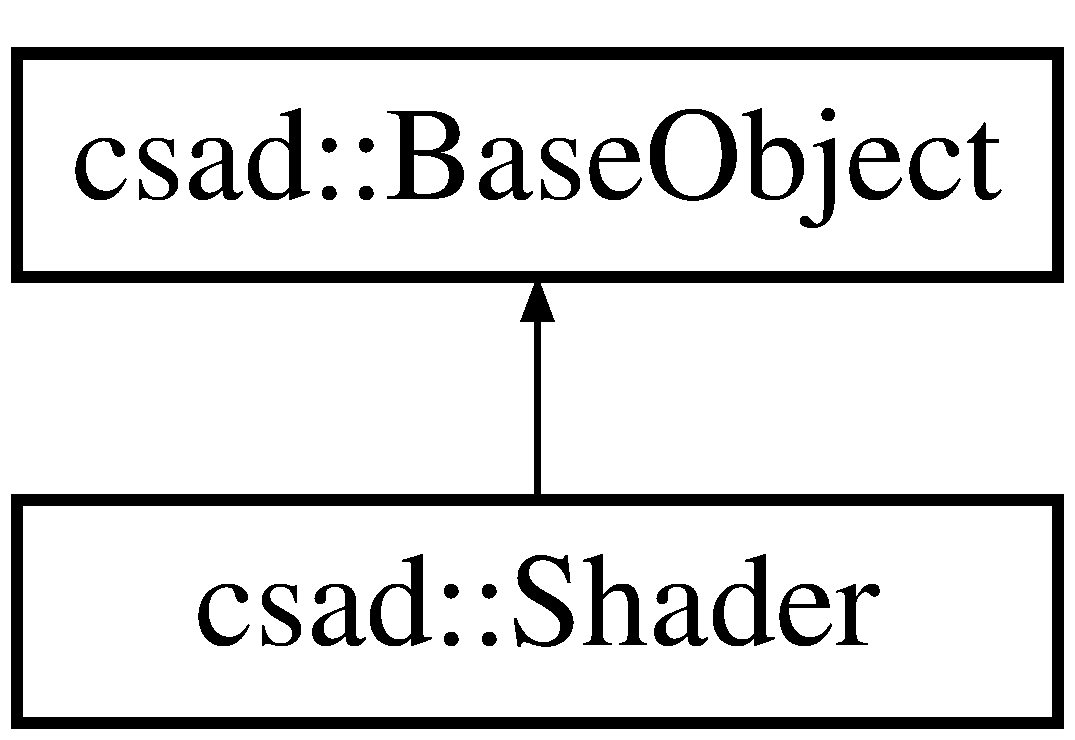
\includegraphics[height=2.000000cm]{classcsad_1_1_shader}
\end{center}
\end{figure}
\subsection*{Public Member Functions}
\begin{DoxyCompactItemize}
\item 
\hypertarget{classcsad_1_1_shader_a5f7e6e5396ee4b432ae118b65ce58446}{C\-S\-A\-D\-\_\-\-A\-P\-I void $\ast$ \hyperlink{classcsad_1_1_shader_a5f7e6e5396ee4b432ae118b65ce58446}{set} (unsigned \-\_\-int32, void $\ast$)}\label{classcsad_1_1_shader_a5f7e6e5396ee4b432ae118b65ce58446}

\begin{DoxyCompactList}\small\item\em used for any interface commands. \end{DoxyCompactList}\end{DoxyCompactItemize}
\subsection*{Additional Inherited Members}


\subsection{Detailed Description}
\hyperlink{classcsad_1_1_shader}{Shader} -\/ the object of shader programm. 

\begin{DoxyVerb}  <Shader name="shader name" />
\end{DoxyVerb}
 \begin{DoxySeeAlso}{See Also}
\hyperlink{group__scene}{csad\-: scene} 
\end{DoxySeeAlso}

\hypertarget{classcsad_1_1_static_mesh}{\section{csad\-:\-:Static\-Mesh Class Reference}
\label{classcsad_1_1_static_mesh}\index{csad\-::\-Static\-Mesh@{csad\-::\-Static\-Mesh}}
}


\hyperlink{classcsad_1_1_static_mesh}{Static\-Mesh} -\/ the class is static geometry.  


Inheritance diagram for csad\-:\-:Static\-Mesh\-:\begin{figure}[H]
\begin{center}
\leavevmode
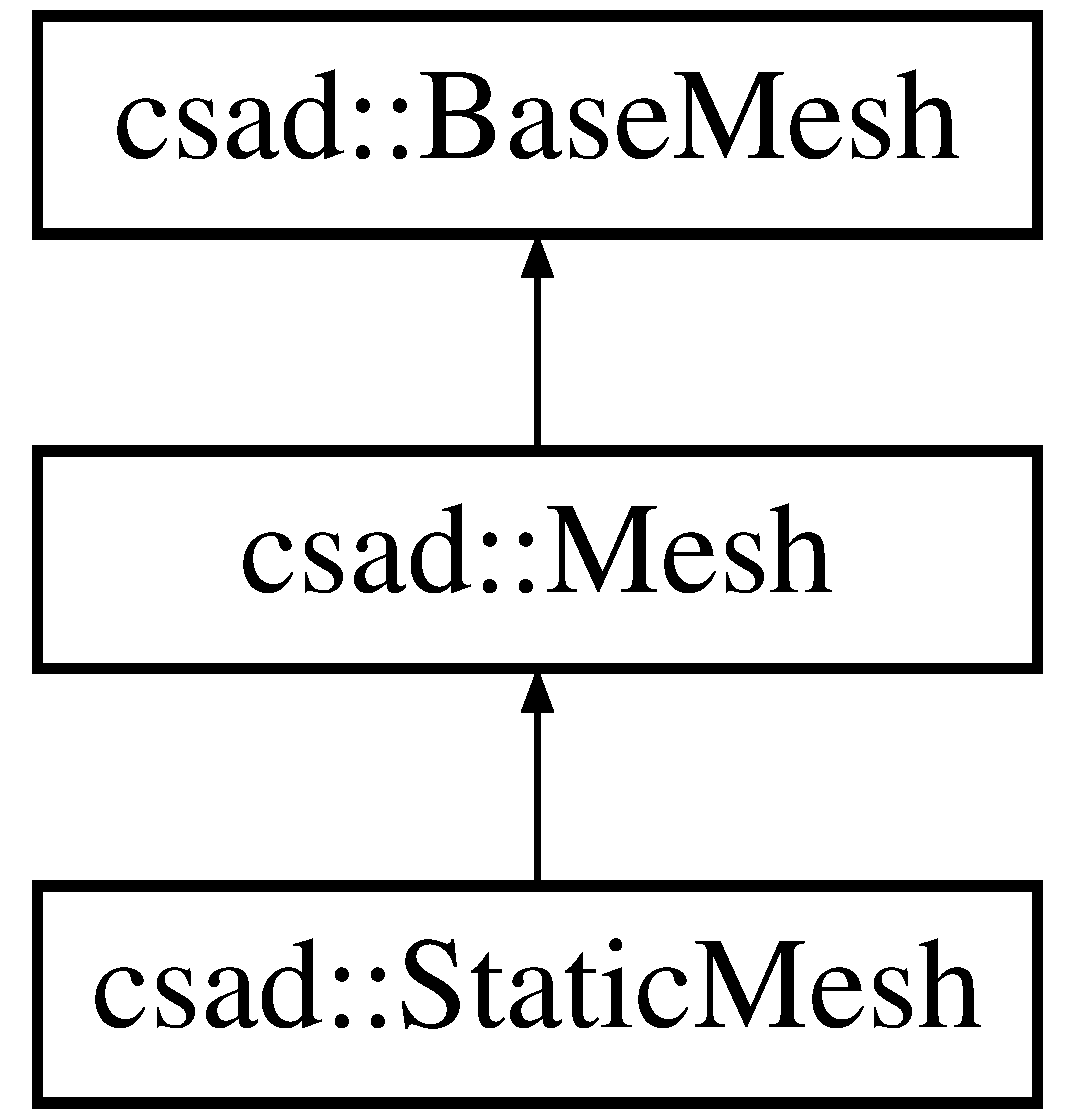
\includegraphics[height=3.000000cm]{classcsad_1_1_static_mesh}
\end{center}
\end{figure}
\subsection*{Additional Inherited Members}


\subsection{Detailed Description}
\hyperlink{classcsad_1_1_static_mesh}{Static\-Mesh} -\/ the class is static geometry. 

\begin{DoxySeeAlso}{See Also}
\hyperlink{group__scene}{csad\-: scene} 
\end{DoxySeeAlso}

\hypertarget{classcsad_1_1_style}{\section{csad\-:\-:Style Class Reference}
\label{classcsad_1_1_style}\index{csad\-::\-Style@{csad\-::\-Style}}
}


\hyperlink{classcsad_1_1_style}{Style} -\/ container styles.  


Inheritance diagram for csad\-:\-:Style\-:\begin{figure}[H]
\begin{center}
\leavevmode
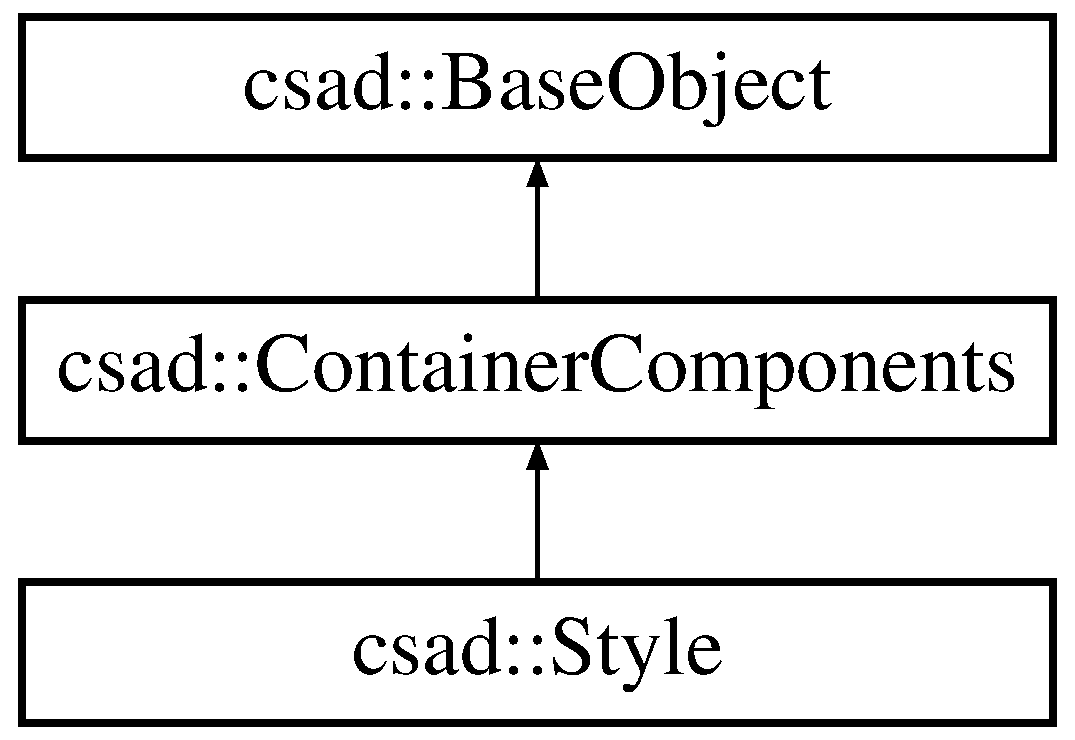
\includegraphics[height=3.000000cm]{classcsad_1_1_style}
\end{center}
\end{figure}
\subsection*{Public Member Functions}
\begin{DoxyCompactItemize}
\item 
\hypertarget{classcsad_1_1_style_abf5aa6a96ac8c40378b8acdafca4875a}{{\footnotesize template$<$typename T $>$ }\\\-\_\-\-F\-O\-R\-C\-E\-I\-N\-L\-I\-N\-E T $\ast$ \hyperlink{classcsad_1_1_style_abf5aa6a96ac8c40378b8acdafca4875a}{get\-Component} ()}\label{classcsad_1_1_style_abf5aa6a96ac8c40378b8acdafca4875a}

\begin{DoxyCompactList}\small\item\em Returns the component of the given type, if it is not in a container returns 0. \end{DoxyCompactList}\item 
\hypertarget{classcsad_1_1_style_a67ccaa9e84a17c49da5dec3b8c78c833}{\-\_\-\-F\-O\-R\-C\-E\-I\-N\-L\-I\-N\-E \hyperlink{classcsad_1_1_component}{Component} $\ast$ \hyperlink{classcsad_1_1_style_a67ccaa9e84a17c49da5dec3b8c78c833}{get\-Component} (void $\ast$t)}\label{classcsad_1_1_style_a67ccaa9e84a17c49da5dec3b8c78c833}

\begin{DoxyCompactList}\small\item\em Returns the component of the given type, if it is not in a container returns 0. \end{DoxyCompactList}\item 
\hypertarget{classcsad_1_1_style_a97213ecf688a3ea39a8d931e3351b211}{C\-S\-A\-D\-\_\-\-A\-P\-I void $\ast$ \hyperlink{classcsad_1_1_style_a97213ecf688a3ea39a8d931e3351b211}{set} (unsigned \-\_\-int32 id, void $\ast$param)}\label{classcsad_1_1_style_a97213ecf688a3ea39a8d931e3351b211}

\begin{DoxyCompactList}\small\item\em used for any interface commands. \end{DoxyCompactList}\end{DoxyCompactItemize}
\subsection*{Additional Inherited Members}


\subsection{Detailed Description}
\hyperlink{classcsad_1_1_style}{Style} -\/ container styles. 

Necessary to create the model of the parameter list. Not tied to a particular environment, allows you to store various components and their parameters for future use. Unlike the base of the container tied to the Manager graphics. You can use any set of components, which contains the necessary settings, which can be the same for a large number of objects. Changing the style settings after you install it in your object, may not always lead to a change of an object that requires a re-\/install of the style object.

For description in the configuration\-: \begin{DoxyVerb}  <Style name="the name of the style">
  ... components ...
  </Style>
\end{DoxyVerb}


\begin{DoxySeeAlso}{See Also}
\hyperlink{group__core}{csad\-: core}, \hyperlink{classcsad_1_1_text_style}{Text\-Style}, \hyperlink{classcsad_1_1_s_g_button_style}{S\-G\-Button\-Style}, \hyperlink{classcsad_1_1_s_g_element_style}{S\-G\-Element\-Style} 
\end{DoxySeeAlso}

\hypertarget{classcsad_1_1_system}{\section{csad\-:\-:System Class Reference}
\label{classcsad_1_1_system}\index{csad\-::\-System@{csad\-::\-System}}
}


\hyperlink{classcsad_1_1_system}{System} -\/ .  




\subsection{Detailed Description}
\hyperlink{classcsad_1_1_system}{System} -\/ . 

\begin{DoxySeeAlso}{See Also}
\hyperlink{group__core}{csad\-: core} 
\end{DoxySeeAlso}

\hypertarget{classcsad_1_1_text3_d}{\section{csad\-:\-:Text3\-D Class Reference}
\label{classcsad_1_1_text3_d}\index{csad\-::\-Text3\-D@{csad\-::\-Text3\-D}}
}


\hyperlink{classcsad_1_1_text3_d}{Text3\-D} -\/ component, is suitable for construction of geometry text. Build output is saved in a \hyperlink{classcsad_1_1_mesh}{Mesh} situated in the component \hyperlink{classcsad_1_1_mesh_filter}{Mesh\-Filter}.  


Inheritance diagram for csad\-:\-:Text3\-D\-:\begin{figure}[H]
\begin{center}
\leavevmode
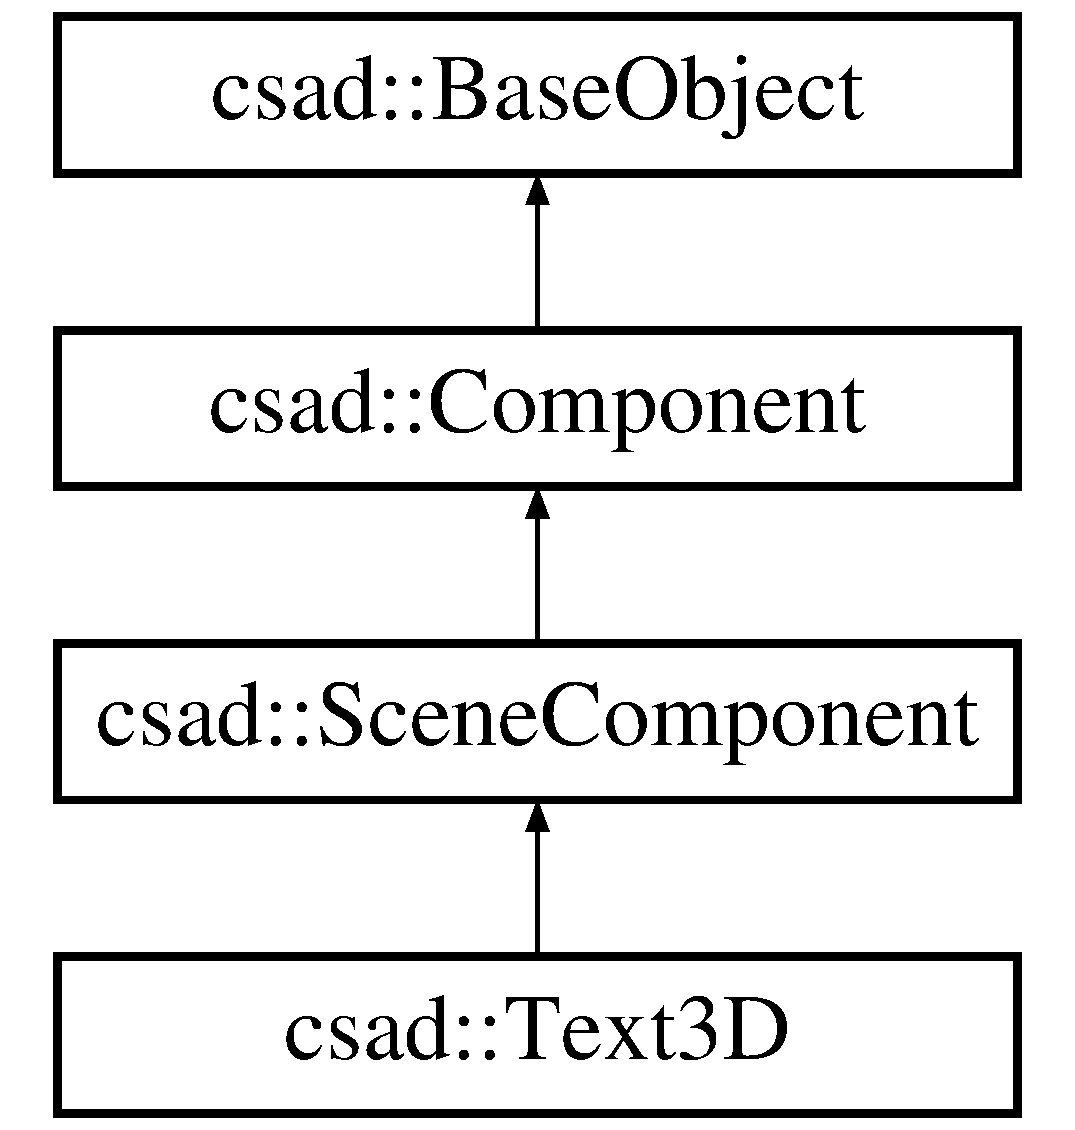
\includegraphics[height=4.000000cm]{classcsad_1_1_text3_d}
\end{center}
\end{figure}
\subsection*{Public Member Functions}
\begin{DoxyCompactItemize}
\item 
\hypertarget{classcsad_1_1_text3_d_ad6137b853b2d674cc34e318bac7abca7}{C\-S\-A\-D\-\_\-\-A\-P\-I void \hyperlink{classcsad_1_1_text3_d_ad6137b853b2d674cc34e318bac7abca7}{quit} ()}\label{classcsad_1_1_text3_d_ad6137b853b2d674cc34e318bac7abca7}

\begin{DoxyCompactList}\small\item\em The event is called before the program exits. \end{DoxyCompactList}\item 
\hypertarget{classcsad_1_1_text3_d_ad92bc8c88734d84afecdc6fb7fcd7d83}{C\-S\-A\-D\-\_\-\-A\-P\-I void $\ast$ \hyperlink{classcsad_1_1_text3_d_ad92bc8c88734d84afecdc6fb7fcd7d83}{set} (unsigned \-\_\-int32, void $\ast$)}\label{classcsad_1_1_text3_d_ad92bc8c88734d84afecdc6fb7fcd7d83}

\begin{DoxyCompactList}\small\item\em used for any interface commands. \end{DoxyCompactList}\item 
\hypertarget{classcsad_1_1_text3_d_a20c5cafb2d194dee028c9536e2ff903f}{C\-S\-A\-D\-\_\-\-A\-P\-I void \hyperlink{classcsad_1_1_text3_d_a20c5cafb2d194dee028c9536e2ff903f}{set\-Offset} (float offset)}\label{classcsad_1_1_text3_d_a20c5cafb2d194dee028c9536e2ff903f}

\begin{DoxyCompactList}\small\item\em To set the offset into the depth. \end{DoxyCompactList}\item 
\hypertarget{classcsad_1_1_text3_d_aaa37c053f2999d9b2c8c45b0380e0204}{C\-S\-A\-D\-\_\-\-A\-P\-I void \hyperlink{classcsad_1_1_text3_d_aaa37c053f2999d9b2c8c45b0380e0204}{set\-Resiver} (\hyperlink{classcsad_1_1_base_object}{Base\-Object} $\ast$)}\label{classcsad_1_1_text3_d_aaa37c053f2999d9b2c8c45b0380e0204}

\begin{DoxyCompactList}\small\item\em sets the object receiving the event from the text \end{DoxyCompactList}\item 
\hypertarget{classcsad_1_1_text3_d_a5a7528171be95e957c2346632801eae3}{C\-S\-A\-D\-\_\-\-A\-P\-I \hyperlink{classcsad_1_1_text3_d}{Text3\-D} \& \hyperlink{classcsad_1_1_text3_d_a5a7528171be95e957c2346632801eae3}{set\-Style} (char $\ast$name)}\label{classcsad_1_1_text3_d_a5a7528171be95e957c2346632801eae3}

\begin{DoxyCompactList}\small\item\em Sets the style of the text style name. \end{DoxyCompactList}\item 
\hypertarget{classcsad_1_1_text3_d_a3b751cd3479ef65127f0b2fe6eb1c81d}{C\-S\-A\-D\-\_\-\-A\-P\-I \hyperlink{classcsad_1_1_text3_d}{Text3\-D} \& \hyperlink{classcsad_1_1_text3_d_a3b751cd3479ef65127f0b2fe6eb1c81d}{set\-Style} (const char $\ast$name)}\label{classcsad_1_1_text3_d_a3b751cd3479ef65127f0b2fe6eb1c81d}

\begin{DoxyCompactList}\small\item\em Sets the style of the text style name. \end{DoxyCompactList}\item 
\hypertarget{classcsad_1_1_text3_d_aef1fbc8c246d1ccb519a8538f680c3b8}{C\-S\-A\-D\-\_\-\-A\-P\-I \hyperlink{classcsad_1_1_text3_d}{Text3\-D} \& \hyperlink{classcsad_1_1_text3_d_aef1fbc8c246d1ccb519a8538f680c3b8}{set\-Style} (\hyperlink{classcsad_1_1_style}{Style} $\ast$style)}\label{classcsad_1_1_text3_d_aef1fbc8c246d1ccb519a8538f680c3b8}

\begin{DoxyCompactList}\small\item\em Sets the style. \end{DoxyCompactList}\item 
\hypertarget{classcsad_1_1_text3_d_aa582e107e181674db00fabad2cc80457}{C\-S\-A\-D\-\_\-\-A\-P\-I \hyperlink{classcsad_1_1_text3_d}{Text3\-D} \& \hyperlink{classcsad_1_1_text3_d_aa582e107e181674db00fabad2cc80457}{set\-Text} (char $\ast$\hyperlink{classcsad_1_1_text3_d_a189ccec8b8310503a73c5ce304e0e557}{text})}\label{classcsad_1_1_text3_d_aa582e107e181674db00fabad2cc80457}

\begin{DoxyCompactList}\small\item\em Sets the text. \end{DoxyCompactList}\item 
\hypertarget{classcsad_1_1_text3_d_ab22949e1eefb67db5234696e9c68af2c}{C\-S\-A\-D\-\_\-\-A\-P\-I \hyperlink{classcsad_1_1_text3_d}{Text3\-D} \& \hyperlink{classcsad_1_1_text3_d_ab22949e1eefb67db5234696e9c68af2c}{set\-Text} (const char $\ast$\hyperlink{classcsad_1_1_text3_d_a189ccec8b8310503a73c5ce304e0e557}{text})}\label{classcsad_1_1_text3_d_ab22949e1eefb67db5234696e9c68af2c}

\begin{DoxyCompactList}\small\item\em Sets the text. \end{DoxyCompactList}\item 
\hypertarget{classcsad_1_1_text3_d_a65b09648882d85a87b83c2d2192374d0}{C\-S\-A\-D\-\_\-\-A\-P\-I void \hyperlink{classcsad_1_1_text3_d_a65b09648882d85a87b83c2d2192374d0}{start} ()}\label{classcsad_1_1_text3_d_a65b09648882d85a87b83c2d2192374d0}

\begin{DoxyCompactList}\small\item\em This event is fired after the program start. \end{DoxyCompactList}\item 
\hypertarget{classcsad_1_1_text3_d_a189ccec8b8310503a73c5ce304e0e557}{\-\_\-\-F\-O\-R\-C\-E\-I\-N\-L\-I\-N\-E const char $\ast$ \hyperlink{classcsad_1_1_text3_d_a189ccec8b8310503a73c5ce304e0e557}{text} ()}\label{classcsad_1_1_text3_d_a189ccec8b8310503a73c5ce304e0e557}

\begin{DoxyCompactList}\small\item\em Restores text. \end{DoxyCompactList}\item 
\hypertarget{classcsad_1_1_text3_d_ae5732773b756bd15ac48ea9d68140f31}{C\-S\-A\-D\-\_\-\-A\-P\-I \hyperlink{classbt_1_1vector3d}{vector3d} \hyperlink{classcsad_1_1_text3_d_ae5732773b756bd15ac48ea9d68140f31}{text\-Center} ()}\label{classcsad_1_1_text3_d_ae5732773b756bd15ac48ea9d68140f31}

\begin{DoxyCompactList}\small\item\em Returns the position of the text. \end{DoxyCompactList}\item 
\hypertarget{classcsad_1_1_text3_d_a428eb4115f5db77815e829a46e83c505}{\-\_\-\-F\-O\-R\-C\-E\-I\-N\-L\-I\-N\-E \hyperlink{classcsad_1_1_text_style}{Text\-Style} $\ast$ \hyperlink{classcsad_1_1_text3_d_a428eb4115f5db77815e829a46e83c505}{text\-Style} ()}\label{classcsad_1_1_text3_d_a428eb4115f5db77815e829a46e83c505}

\begin{DoxyCompactList}\small\item\em Returns the text style. \end{DoxyCompactList}\item 
\hypertarget{classcsad_1_1_text3_d_ac10717fb94ba35cb7a2d02ce06edaa03}{C\-S\-A\-D\-\_\-\-A\-P\-I void \hyperlink{classcsad_1_1_text3_d_ac10717fb94ba35cb7a2d02ce06edaa03}{update} ()}\label{classcsad_1_1_text3_d_ac10717fb94ba35cb7a2d02ce06edaa03}

\begin{DoxyCompactList}\small\item\em This event is fired before rendering environment container component. \end{DoxyCompactList}\end{DoxyCompactItemize}
\subsection*{Additional Inherited Members}


\subsection{Detailed Description}
\hyperlink{classcsad_1_1_text3_d}{Text3\-D} -\/ component, is suitable for construction of geometry text. Build output is saved in a \hyperlink{classcsad_1_1_mesh}{Mesh} situated in the component \hyperlink{classcsad_1_1_mesh_filter}{Mesh\-Filter}. 

\begin{DoxySeeAlso}{See Also}
\hyperlink{group__scene}{csad\-: scene} \hyperlink{classcsad_1_1_mesh_filter}{Mesh\-Filter} \hyperlink{classcsad_1_1_mesh}{Mesh} 
\end{DoxySeeAlso}

\hypertarget{classcsad_1_1_text_style}{\section{csad\-:\-:Text\-Style Class Reference}
\label{classcsad_1_1_text_style}\index{csad\-::\-Text\-Style@{csad\-::\-Text\-Style}}
}


\hyperlink{classcsad_1_1_text_style}{Text\-Style} -\/ component describing the parameters of the text.  


Inheritance diagram for csad\-:\-:Text\-Style\-:\begin{figure}[H]
\begin{center}
\leavevmode
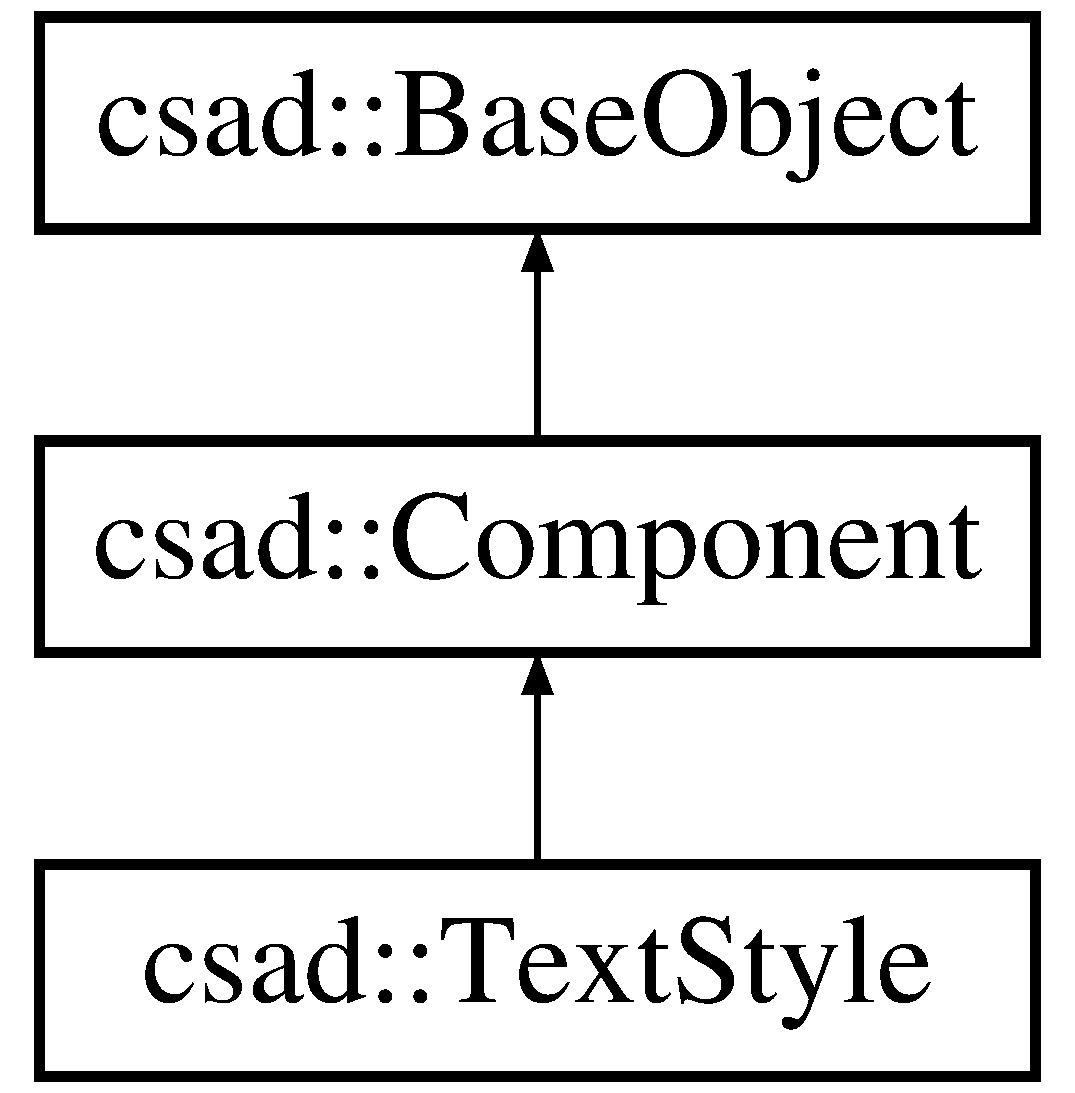
\includegraphics[height=3.000000cm]{classcsad_1_1_text_style}
\end{center}
\end{figure}
\subsection*{Public Types}
\begin{DoxyCompactItemize}
\item 
enum \hyperlink{classcsad_1_1_text_style_aacdb2bdc2e607a6106be8120b932e47d}{Anchor} \{ \\*
\hyperlink{classcsad_1_1_text_style_aacdb2bdc2e607a6106be8120b932e47da763ab2a048994f7b96589a3d0f26d094}{Top} = 0x010, 
\hyperlink{classcsad_1_1_text_style_aacdb2bdc2e607a6106be8120b932e47da2361aedcdae29d6a4e4ab381f587cd0c}{Center} = 0x000, 
\hyperlink{classcsad_1_1_text_style_aacdb2bdc2e607a6106be8120b932e47da81e426475315efe4103acea301edb012}{Bottom} = 0x020, 
\hyperlink{classcsad_1_1_text_style_aacdb2bdc2e607a6106be8120b932e47da51aa1a1e321e5b6237aa59e65aecb1cf}{Left} = 0x100, 
\\*
\hyperlink{classcsad_1_1_text_style_aacdb2bdc2e607a6106be8120b932e47da6db0b3d20d2eb5faaa4a5f7cd675282f}{Right} = 0x001, 
\hyperlink{classcsad_1_1_text_style_aacdb2bdc2e607a6106be8120b932e47da9f825017d1633a4f44e96ad73023b067}{Left\-\_\-\-Top} = 0x110, 
\hyperlink{classcsad_1_1_text_style_aacdb2bdc2e607a6106be8120b932e47da01c6392be426c84ddfa59864178f7df4}{Left\-\_\-\-Center} = 0x100, 
\hyperlink{classcsad_1_1_text_style_aacdb2bdc2e607a6106be8120b932e47da976ad443e03acbc053c96d302048ecdd}{Left\-\_\-\-Bottom} = 0x120, 
\\*
\hyperlink{classcsad_1_1_text_style_aacdb2bdc2e607a6106be8120b932e47da22b03a7d736b6bacbcacc04b92483e35}{Right\-\_\-\-Top} = 0x011, 
\hyperlink{classcsad_1_1_text_style_aacdb2bdc2e607a6106be8120b932e47da6f79ccb724936f4a80d1ce1060623ad5}{Right\-\_\-\-Center} = 0x001, 
\hyperlink{classcsad_1_1_text_style_aacdb2bdc2e607a6106be8120b932e47da7afd942bb03db116f44e1995d92e259b}{Right\-\_\-\-Bottom} = 0x021
 \}
\end{DoxyCompactItemize}
\subsection*{Public Member Functions}
\begin{DoxyCompactItemize}
\item 
\hypertarget{classcsad_1_1_text_style_ae640d6150ed81fc5283ead658cceadf4}{\-\_\-\-F\-O\-R\-C\-E\-I\-N\-L\-I\-N\-E int \hyperlink{classcsad_1_1_text_style_ae640d6150ed81fc5283ead658cceadf4}{get\-Anchor} ()}\label{classcsad_1_1_text_style_ae640d6150ed81fc5283ead658cceadf4}

\begin{DoxyCompactList}\small\item\em Returns the orientation of the text. \end{DoxyCompactList}\item 
\hypertarget{classcsad_1_1_text_style_aa0b2339391c3902a7738492d112f9e91}{\-\_\-\-F\-O\-R\-C\-E\-I\-N\-L\-I\-N\-E float \hyperlink{classcsad_1_1_text_style_aa0b2339391c3902a7738492d112f9e91}{get\-Char\-Size} ()}\label{classcsad_1_1_text_style_aa0b2339391c3902a7738492d112f9e91}

\begin{DoxyCompactList}\small\item\em Returns the scale of the image characters. \end{DoxyCompactList}\item 
\-\_\-\-F\-O\-R\-C\-E\-I\-N\-L\-I\-N\-E \hyperlink{classcsad_1_1_font}{Font} $\ast$ \hyperlink{classcsad_1_1_text_style_a29e755e840f031d4a495c01377016cf6}{get\-Font} ()
\item 
\hypertarget{classcsad_1_1_text_style_a27e23126f471f26f7c8459b3681cdad0}{\-\_\-\-F\-O\-R\-C\-E\-I\-N\-L\-I\-N\-E float \hyperlink{classcsad_1_1_text_style_a27e23126f471f26f7c8459b3681cdad0}{get\-Kerning} ()}\label{classcsad_1_1_text_style_a27e23126f471f26f7c8459b3681cdad0}

\begin{DoxyCompactList}\small\item\em Returns the scale of the character spacing. \end{DoxyCompactList}\item 
\hypertarget{classcsad_1_1_text_style_a2cc19f704b21124f5cb7629006984e9f}{\-\_\-\-F\-O\-R\-C\-E\-I\-N\-L\-I\-N\-E \hyperlink{classcsad_1_1_material}{Material} $\ast$ \hyperlink{classcsad_1_1_text_style_a2cc19f704b21124f5cb7629006984e9f}{get\-Matrial} ()}\label{classcsad_1_1_text_style_a2cc19f704b21124f5cb7629006984e9f}

\begin{DoxyCompactList}\small\item\em Returns an object of material. \end{DoxyCompactList}\item 
\hypertarget{classcsad_1_1_text_style_aa1f96fcb68ee340eed28c795fd7b0fdd}{C\-S\-A\-D\-\_\-\-A\-P\-I void $\ast$ \hyperlink{classcsad_1_1_text_style_aa1f96fcb68ee340eed28c795fd7b0fdd}{set} (unsigned \-\_\-int32, void $\ast$)}\label{classcsad_1_1_text_style_aa1f96fcb68ee340eed28c795fd7b0fdd}

\begin{DoxyCompactList}\small\item\em used for any interface commands. \end{DoxyCompactList}\item 
\hypertarget{classcsad_1_1_text_style_af16a9581629ca0037478dbaa9a4377c5}{C\-S\-A\-D\-\_\-\-A\-P\-I \hyperlink{classcsad_1_1_text_style}{Text\-Style} \& \hyperlink{classcsad_1_1_text_style_af16a9581629ca0037478dbaa9a4377c5}{set\-Anchor} (char $\ast$name)}\label{classcsad_1_1_text_style_af16a9581629ca0037478dbaa9a4377c5}

\begin{DoxyCompactList}\small\item\em Specifies the orientation of the text by name. \end{DoxyCompactList}\item 
\hypertarget{classcsad_1_1_text_style_a043ba2c648388f8f7269a2a5be9321bb}{C\-S\-A\-D\-\_\-\-A\-P\-I \hyperlink{classcsad_1_1_text_style}{Text\-Style} \& \hyperlink{classcsad_1_1_text_style_a043ba2c648388f8f7269a2a5be9321bb}{set\-Anchor} (int val)}\label{classcsad_1_1_text_style_a043ba2c648388f8f7269a2a5be9321bb}

\begin{DoxyCompactList}\small\item\em Specifies the orientation of the text. \end{DoxyCompactList}\item 
\hypertarget{classcsad_1_1_text_style_a1be6d97cc420d2c798e514d51491045a}{C\-S\-A\-D\-\_\-\-A\-P\-I \hyperlink{classcsad_1_1_text_style}{Text\-Style} \& \hyperlink{classcsad_1_1_text_style_a1be6d97cc420d2c798e514d51491045a}{set\-Char\-Size} (float val)}\label{classcsad_1_1_text_style_a1be6d97cc420d2c798e514d51491045a}

\begin{DoxyCompactList}\small\item\em Specifies the scale of the image characters. \end{DoxyCompactList}\item 
\hypertarget{classcsad_1_1_text_style_acac87e88c6e26886fd4e6a926029659a}{C\-S\-A\-D\-\_\-\-A\-P\-I \hyperlink{classcsad_1_1_text_style}{Text\-Style} \& \hyperlink{classcsad_1_1_text_style_acac87e88c6e26886fd4e6a926029659a}{set\-Font} (char $\ast$path)}\label{classcsad_1_1_text_style_acac87e88c6e26886fd4e6a926029659a}

\begin{DoxyCompactList}\small\item\em Sets the font for the server name and font. \end{DoxyCompactList}\item 
\hypertarget{classcsad_1_1_text_style_a6f824301e998e89906f260faa48f86ee}{\-\_\-\-F\-O\-R\-C\-E\-I\-N\-L\-I\-N\-E \hyperlink{classcsad_1_1_text_style}{Text\-Style} \& \hyperlink{classcsad_1_1_text_style_a6f824301e998e89906f260faa48f86ee}{set\-Font} (const char $\ast$path)}\label{classcsad_1_1_text_style_a6f824301e998e89906f260faa48f86ee}

\begin{DoxyCompactList}\small\item\em Sets the font for the server name and font. \end{DoxyCompactList}\item 
\hypertarget{classcsad_1_1_text_style_a5df3970f5c726e6dfb0263f153ec7e9b}{C\-S\-A\-D\-\_\-\-A\-P\-I \hyperlink{classcsad_1_1_text_style}{Text\-Style} \& \hyperlink{classcsad_1_1_text_style_a5df3970f5c726e6dfb0263f153ec7e9b}{set\-Font} (\hyperlink{classcsad_1_1_font}{Font} $\ast$font)}\label{classcsad_1_1_text_style_a5df3970f5c726e6dfb0263f153ec7e9b}

\begin{DoxyCompactList}\small\item\em Specifies the font object. \end{DoxyCompactList}\item 
\hypertarget{classcsad_1_1_text_style_aa5f55fddbde4fa1d88da5f578c81bf4b}{C\-S\-A\-D\-\_\-\-A\-P\-I \hyperlink{classcsad_1_1_text_style}{Text\-Style} \& \hyperlink{classcsad_1_1_text_style_aa5f55fddbde4fa1d88da5f578c81bf4b}{set\-Kerning} (float val)}\label{classcsad_1_1_text_style_aa5f55fddbde4fa1d88da5f578c81bf4b}

\begin{DoxyCompactList}\small\item\em Specifies the scale of the distance between characters. \end{DoxyCompactList}\item 
\hypertarget{classcsad_1_1_text_style_a15a3570f3ca090453331953226e72464}{C\-S\-A\-D\-\_\-\-A\-P\-I \hyperlink{classcsad_1_1_text_style}{Text\-Style} \& \hyperlink{classcsad_1_1_text_style_a15a3570f3ca090453331953226e72464}{set\-Material} (char $\ast$name)}\label{classcsad_1_1_text_style_a15a3570f3ca090453331953226e72464}

\begin{DoxyCompactList}\small\item\em Specifies the material by name. \end{DoxyCompactList}\item 
\hypertarget{classcsad_1_1_text_style_afc4e3ed006f391f10b412d390181654c}{C\-S\-A\-D\-\_\-\-A\-P\-I \hyperlink{classcsad_1_1_text_style}{Text\-Style} \& \hyperlink{classcsad_1_1_text_style_afc4e3ed006f391f10b412d390181654c}{set\-Material} (\hyperlink{classcsad_1_1_material}{Material} $\ast$mat)}\label{classcsad_1_1_text_style_afc4e3ed006f391f10b412d390181654c}

\begin{DoxyCompactList}\small\item\em Sets the object's material. \end{DoxyCompactList}\end{DoxyCompactItemize}
\subsection*{Additional Inherited Members}


\subsection{Detailed Description}
\hyperlink{classcsad_1_1_text_style}{Text\-Style} -\/ component describing the parameters of the text. 

For description in the configuration\-: \begin{DoxyVerb}  <Style name="the name of the style">
     <TextStyle font="server/font" material="textMaterial" charsize="0.0005" kerning="1.0" />
  </Style>
\end{DoxyVerb}


\begin{DoxySeeAlso}{See Also}
\hyperlink{group__scene}{csad\-: scene} 
\end{DoxySeeAlso}


\subsection{Member Enumeration Documentation}
\hypertarget{classcsad_1_1_text_style_aacdb2bdc2e607a6106be8120b932e47d}{\index{csad\-::\-Text\-Style@{csad\-::\-Text\-Style}!Anchor@{Anchor}}
\index{Anchor@{Anchor}!csad::TextStyle@{csad\-::\-Text\-Style}}
\subsubsection[{Anchor}]{\setlength{\rightskip}{0pt plus 5cm}enum {\bf csad\-::\-Text\-Style\-::\-Anchor}}}\label{classcsad_1_1_text_style_aacdb2bdc2e607a6106be8120b932e47d}
\begin{Desc}
\item[Enumerator]\par
\begin{description}
\index{Top@{Top}!csad\-::\-Text\-Style@{csad\-::\-Text\-Style}}\index{csad\-::\-Text\-Style@{csad\-::\-Text\-Style}!Top@{Top}}\item[{\em 
\hypertarget{classcsad_1_1_text_style_aacdb2bdc2e607a6106be8120b932e47da763ab2a048994f7b96589a3d0f26d094}{Top}\label{classcsad_1_1_text_style_aacdb2bdc2e607a6106be8120b932e47da763ab2a048994f7b96589a3d0f26d094}
}]on top \index{Center@{Center}!csad\-::\-Text\-Style@{csad\-::\-Text\-Style}}\index{csad\-::\-Text\-Style@{csad\-::\-Text\-Style}!Center@{Center}}\item[{\em 
\hypertarget{classcsad_1_1_text_style_aacdb2bdc2e607a6106be8120b932e47da2361aedcdae29d6a4e4ab381f587cd0c}{Center}\label{classcsad_1_1_text_style_aacdb2bdc2e607a6106be8120b932e47da2361aedcdae29d6a4e4ab381f587cd0c}
}]on center \index{Bottom@{Bottom}!csad\-::\-Text\-Style@{csad\-::\-Text\-Style}}\index{csad\-::\-Text\-Style@{csad\-::\-Text\-Style}!Bottom@{Bottom}}\item[{\em 
\hypertarget{classcsad_1_1_text_style_aacdb2bdc2e607a6106be8120b932e47da81e426475315efe4103acea301edb012}{Bottom}\label{classcsad_1_1_text_style_aacdb2bdc2e607a6106be8120b932e47da81e426475315efe4103acea301edb012}
}]relative to the bottom \index{Left@{Left}!csad\-::\-Text\-Style@{csad\-::\-Text\-Style}}\index{csad\-::\-Text\-Style@{csad\-::\-Text\-Style}!Left@{Left}}\item[{\em 
\hypertarget{classcsad_1_1_text_style_aacdb2bdc2e607a6106be8120b932e47da51aa1a1e321e5b6237aa59e65aecb1cf}{Left}\label{classcsad_1_1_text_style_aacdb2bdc2e607a6106be8120b932e47da51aa1a1e321e5b6237aa59e65aecb1cf}
}]относительно лева \index{Right@{Right}!csad\-::\-Text\-Style@{csad\-::\-Text\-Style}}\index{csad\-::\-Text\-Style@{csad\-::\-Text\-Style}!Right@{Right}}\item[{\em 
\hypertarget{classcsad_1_1_text_style_aacdb2bdc2e607a6106be8120b932e47da6db0b3d20d2eb5faaa4a5f7cd675282f}{Right}\label{classcsad_1_1_text_style_aacdb2bdc2e607a6106be8120b932e47da6db0b3d20d2eb5faaa4a5f7cd675282f}
}]относительно права \index{Left\-\_\-\-Top@{Left\-\_\-\-Top}!csad\-::\-Text\-Style@{csad\-::\-Text\-Style}}\index{csad\-::\-Text\-Style@{csad\-::\-Text\-Style}!Left\-\_\-\-Top@{Left\-\_\-\-Top}}\item[{\em 
\hypertarget{classcsad_1_1_text_style_aacdb2bdc2e607a6106be8120b932e47da9f825017d1633a4f44e96ad73023b067}{Left\-\_\-\-Top}\label{classcsad_1_1_text_style_aacdb2bdc2e607a6106be8120b932e47da9f825017d1633a4f44e96ad73023b067}
}]относительно левого верхнего угла \index{Left\-\_\-\-Center@{Left\-\_\-\-Center}!csad\-::\-Text\-Style@{csad\-::\-Text\-Style}}\index{csad\-::\-Text\-Style@{csad\-::\-Text\-Style}!Left\-\_\-\-Center@{Left\-\_\-\-Center}}\item[{\em 
\hypertarget{classcsad_1_1_text_style_aacdb2bdc2e607a6106be8120b932e47da01c6392be426c84ddfa59864178f7df4}{Left\-\_\-\-Center}\label{classcsad_1_1_text_style_aacdb2bdc2e607a6106be8120b932e47da01c6392be426c84ddfa59864178f7df4}
}]относительно лева по центру \index{Left\-\_\-\-Bottom@{Left\-\_\-\-Bottom}!csad\-::\-Text\-Style@{csad\-::\-Text\-Style}}\index{csad\-::\-Text\-Style@{csad\-::\-Text\-Style}!Left\-\_\-\-Bottom@{Left\-\_\-\-Bottom}}\item[{\em 
\hypertarget{classcsad_1_1_text_style_aacdb2bdc2e607a6106be8120b932e47da976ad443e03acbc053c96d302048ecdd}{Left\-\_\-\-Bottom}\label{classcsad_1_1_text_style_aacdb2bdc2e607a6106be8120b932e47da976ad443e03acbc053c96d302048ecdd}
}]относительно левого нижнего угла \index{Right\-\_\-\-Top@{Right\-\_\-\-Top}!csad\-::\-Text\-Style@{csad\-::\-Text\-Style}}\index{csad\-::\-Text\-Style@{csad\-::\-Text\-Style}!Right\-\_\-\-Top@{Right\-\_\-\-Top}}\item[{\em 
\hypertarget{classcsad_1_1_text_style_aacdb2bdc2e607a6106be8120b932e47da22b03a7d736b6bacbcacc04b92483e35}{Right\-\_\-\-Top}\label{classcsad_1_1_text_style_aacdb2bdc2e607a6106be8120b932e47da22b03a7d736b6bacbcacc04b92483e35}
}]относительно правого верхнего угла \index{Right\-\_\-\-Center@{Right\-\_\-\-Center}!csad\-::\-Text\-Style@{csad\-::\-Text\-Style}}\index{csad\-::\-Text\-Style@{csad\-::\-Text\-Style}!Right\-\_\-\-Center@{Right\-\_\-\-Center}}\item[{\em 
\hypertarget{classcsad_1_1_text_style_aacdb2bdc2e607a6106be8120b932e47da6f79ccb724936f4a80d1ce1060623ad5}{Right\-\_\-\-Center}\label{classcsad_1_1_text_style_aacdb2bdc2e607a6106be8120b932e47da6f79ccb724936f4a80d1ce1060623ad5}
}]относительно права по центру \index{Right\-\_\-\-Bottom@{Right\-\_\-\-Bottom}!csad\-::\-Text\-Style@{csad\-::\-Text\-Style}}\index{csad\-::\-Text\-Style@{csad\-::\-Text\-Style}!Right\-\_\-\-Bottom@{Right\-\_\-\-Bottom}}\item[{\em 
\hypertarget{classcsad_1_1_text_style_aacdb2bdc2e607a6106be8120b932e47da7afd942bb03db116f44e1995d92e259b}{Right\-\_\-\-Bottom}\label{classcsad_1_1_text_style_aacdb2bdc2e607a6106be8120b932e47da7afd942bb03db116f44e1995d92e259b}
}]относительно правого нижнего угла \end{description}
\end{Desc}


\subsection{Member Function Documentation}
\hypertarget{classcsad_1_1_text_style_a29e755e840f031d4a495c01377016cf6}{\index{csad\-::\-Text\-Style@{csad\-::\-Text\-Style}!get\-Font@{get\-Font}}
\index{get\-Font@{get\-Font}!csad::TextStyle@{csad\-::\-Text\-Style}}
\subsubsection[{get\-Font}]{\setlength{\rightskip}{0pt plus 5cm}\-\_\-\-F\-O\-R\-C\-E\-I\-N\-L\-I\-N\-E {\bf Font}$\ast$ csad\-::\-Text\-Style\-::get\-Font (
\begin{DoxyParamCaption}
{}
\end{DoxyParamCaption}
)\hspace{0.3cm}{\ttfamily [inline]}}}\label{classcsad_1_1_text_style_a29e755e840f031d4a495c01377016cf6}
Returns a font object \begin{DoxyReturn}{Returns}
\hyperlink{classcsad_1_1_font}{Font}. 
\end{DoxyReturn}

\hypertarget{classcsad_1_1_texture2_d}{\section{csad\-:\-:Texture2\-D Class Reference}
\label{classcsad_1_1_texture2_d}\index{csad\-::\-Texture2\-D@{csad\-::\-Texture2\-D}}
}


\hyperlink{classcsad_1_1_texture2_d}{Texture2\-D} -\/ two-\/dimensional texture.  


Inheritance diagram for csad\-:\-:Texture2\-D\-:\begin{figure}[H]
\begin{center}
\leavevmode
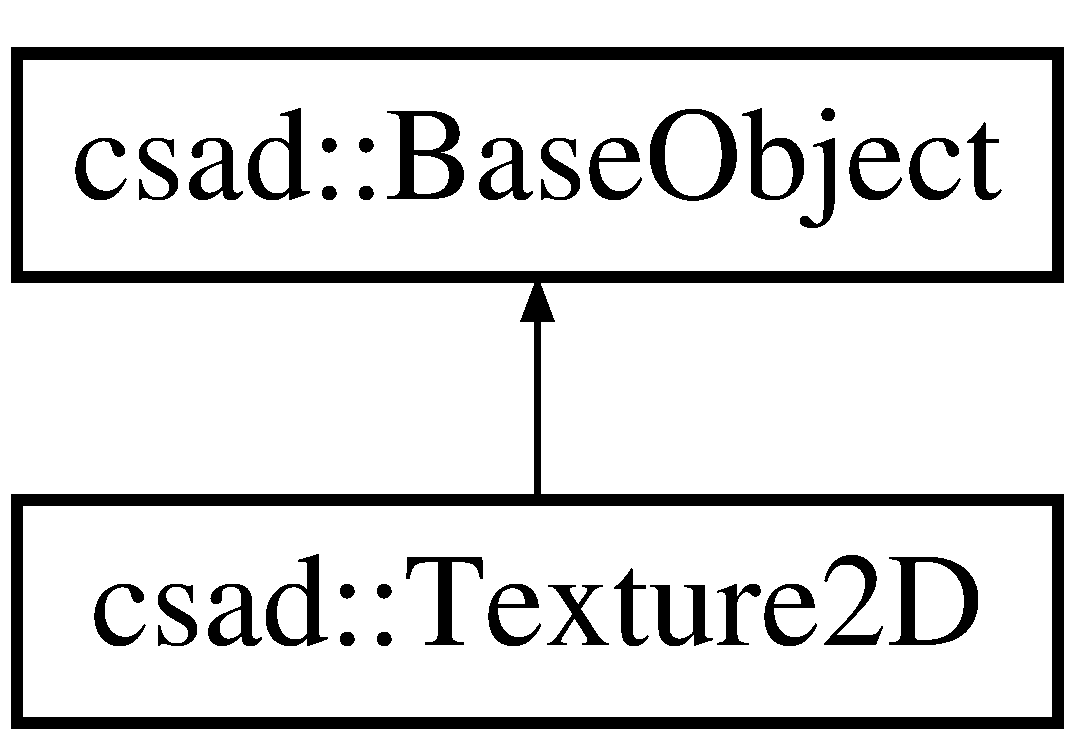
\includegraphics[height=2.000000cm]{classcsad_1_1_texture2_d}
\end{center}
\end{figure}
\subsection*{Public Types}
\begin{DoxyCompactItemize}
\item 
enum \hyperlink{classcsad_1_1_texture2_d_aa1626a57afdd94d1a9cbce5628e81e39}{F\-I\-L\-T\-E\-R} \{ \hyperlink{classcsad_1_1_texture2_d_aa1626a57afdd94d1a9cbce5628e81e39a597a700ee3ef5308bf955fb0934eca69}{normal} = 0x000, 
\hyperlink{classcsad_1_1_texture2_d_aa1626a57afdd94d1a9cbce5628e81e39ae7319b4ef26324e97e6c7904fa57144d}{bilinear} = 0x101
, \hyperlink{classcsad_1_1_texture2_d_aa1626a57afdd94d1a9cbce5628e81e39a5de2d9e733b93f483acb0d648d9d37b3}{trilinear} = 0x105
 \}
\begin{DoxyCompactList}\small\item\em the texture filter \end{DoxyCompactList}\end{DoxyCompactItemize}
\subsection*{Public Member Functions}
\begin{DoxyCompactItemize}
\item 
\hypertarget{classcsad_1_1_texture2_d_aa590b91f8d57eab67019a0de5b2de623}{C\-S\-A\-D\-\_\-\-A\-P\-I void \hyperlink{classcsad_1_1_texture2_d_aa590b91f8d57eab67019a0de5b2de623}{bind} ()}\label{classcsad_1_1_texture2_d_aa590b91f8d57eab67019a0de5b2de623}

\begin{DoxyCompactList}\small\item\em activation of the texture, if the texture was not created when creating or changing a context is created in a new way. \end{DoxyCompactList}\item 
\hypertarget{classcsad_1_1_texture2_d_a32c50d44b46762a79df4d93039f75119}{\-\_\-\-F\-O\-R\-C\-E\-I\-N\-L\-I\-N\-E \hyperlink{classcsad_1_1_gl_context}{Gl\-Context} $\ast$ \hyperlink{classcsad_1_1_texture2_d_a32c50d44b46762a79df4d93039f75119}{context} ()}\label{classcsad_1_1_texture2_d_a32c50d44b46762a79df4d93039f75119}

\begin{DoxyCompactList}\small\item\em the current context, which was used texture. \end{DoxyCompactList}\item 
\hypertarget{classcsad_1_1_texture2_d_a22b7ca01a62e3527d9651ea78d485292}{C\-S\-A\-D\-\_\-\-A\-P\-I void \hyperlink{classcsad_1_1_texture2_d_a22b7ca01a62e3527d9651ea78d485292}{full\-Update} ()}\label{classcsad_1_1_texture2_d_a22b7ca01a62e3527d9651ea78d485292}

\begin{DoxyCompactList}\small\item\em deferred update textures \end{DoxyCompactList}\item 
\hypertarget{classcsad_1_1_texture2_d_a3fd3d4b2b3d62497a58d6177c5886bab}{C\-S\-A\-D\-\_\-\-A\-P\-I int \hyperlink{classcsad_1_1_texture2_d_a3fd3d4b2b3d62497a58d6177c5886bab}{get\-Height} (int level)}\label{classcsad_1_1_texture2_d_a3fd3d4b2b3d62497a58d6177c5886bab}

\begin{DoxyCompactList}\small\item\em return height \end{DoxyCompactList}\item 
\hypertarget{classcsad_1_1_texture2_d_a696f061ccedcb03fe3fe8c86e1092d68}{C\-S\-A\-D\-\_\-\-A\-P\-I const char $\ast$ \hyperlink{classcsad_1_1_texture2_d_a696f061ccedcb03fe3fe8c86e1092d68}{get\-Name} ()}\label{classcsad_1_1_texture2_d_a696f061ccedcb03fe3fe8c86e1092d68}

\begin{DoxyCompactList}\small\item\em returns the name of the texture \end{DoxyCompactList}\item 
\hypertarget{classcsad_1_1_texture2_d_a0d71fbe8b8296da9b3bc2801b10259e7}{C\-S\-A\-D\-\_\-\-A\-P\-I gen\-::\-Raster $\ast$ \hyperlink{classcsad_1_1_texture2_d_a0d71fbe8b8296da9b3bc2801b10259e7}{get\-Raster} ()}\label{classcsad_1_1_texture2_d_a0d71fbe8b8296da9b3bc2801b10259e7}

\begin{DoxyCompactList}\small\item\em returns a resource established as a texture image \end{DoxyCompactList}\item 
\hypertarget{classcsad_1_1_texture2_d_af86e14a234c9a6da93eb805f6e2691ec}{C\-S\-A\-D\-\_\-\-A\-P\-I int \hyperlink{classcsad_1_1_texture2_d_af86e14a234c9a6da93eb805f6e2691ec}{get\-Width} (int level)}\label{classcsad_1_1_texture2_d_af86e14a234c9a6da93eb805f6e2691ec}

\begin{DoxyCompactList}\small\item\em return width \end{DoxyCompactList}\item 
\hypertarget{classcsad_1_1_texture2_d_a3dca71cef5aec246fed9929f0dc4b237}{C\-S\-A\-D\-\_\-\-A\-P\-I void \hyperlink{classcsad_1_1_texture2_d_a3dca71cef5aec246fed9929f0dc4b237}{load} (char $\ast$name)}\label{classcsad_1_1_texture2_d_a3dca71cef5aec246fed9929f0dc4b237}

\begin{DoxyCompactList}\small\item\em download raster file. \end{DoxyCompactList}\item 
\hypertarget{classcsad_1_1_texture2_d_aef53e63cfc69c07ad89dc7a36c7d6ba7}{C\-S\-A\-D\-\_\-\-A\-P\-I void $\ast$ \hyperlink{classcsad_1_1_texture2_d_aef53e63cfc69c07ad89dc7a36c7d6ba7}{set} (unsigned \-\_\-int32, void $\ast$)}\label{classcsad_1_1_texture2_d_aef53e63cfc69c07ad89dc7a36c7d6ba7}

\begin{DoxyCompactList}\small\item\em used for any interface commands. \end{DoxyCompactList}\item 
\hypertarget{classcsad_1_1_texture2_d_aacb2b9c5b55aba437a1c342ec67c301a}{C\-S\-A\-D\-\_\-\-A\-P\-I unsigned int \hyperlink{classcsad_1_1_texture2_d_aacb2b9c5b55aba437a1c342ec67c301a}{set\-Context} (\hyperlink{classcsad_1_1_gl_context}{Gl\-Context} $\ast$\hyperlink{classcsad_1_1_texture2_d_a32c50d44b46762a79df4d93039f75119}{context})}\label{classcsad_1_1_texture2_d_aacb2b9c5b55aba437a1c342ec67c301a}

\begin{DoxyCompactList}\small\item\em returns the number of the texture to the selected context. \end{DoxyCompactList}\item 
\hypertarget{classcsad_1_1_texture2_d_a0ed6920fb8f2fad4086d0a3c7238196a}{C\-S\-A\-D\-\_\-\-A\-P\-I void \hyperlink{classcsad_1_1_texture2_d_a0ed6920fb8f2fad4086d0a3c7238196a}{set\-Raster} (\hyperlink{struct_raster}{Raster} $\ast$raster)}\label{classcsad_1_1_texture2_d_a0ed6920fb8f2fad4086d0a3c7238196a}

\begin{DoxyCompactList}\small\item\em sets the link in the resource would have been born matix texture image \end{DoxyCompactList}\item 
\hypertarget{classcsad_1_1_texture2_d_abade1baf609052a87482c352e7bb7199}{\-\_\-\-F\-O\-R\-C\-E\-I\-N\-L\-I\-N\-E unsigned int \hyperlink{classcsad_1_1_texture2_d_abade1baf609052a87482c352e7bb7199}{texture} ()}\label{classcsad_1_1_texture2_d_abade1baf609052a87482c352e7bb7199}

\begin{DoxyCompactList}\small\item\em I\-D textures for the current context. \end{DoxyCompactList}\item 
\hypertarget{classcsad_1_1_texture2_d_a1e6484cf1cf507fab645af92d782b4f0}{C\-S\-A\-D\-\_\-\-A\-P\-I void \hyperlink{classcsad_1_1_texture2_d_a1e6484cf1cf507fab645af92d782b4f0}{update\-Rect} (\hyperlink{classbt_1_1vector4i}{bt\-::vector4i} $\ast$r, \hyperlink{struct_raster}{Raster} $\ast$raster)}\label{classcsad_1_1_texture2_d_a1e6484cf1cf507fab645af92d782b4f0}

\begin{DoxyCompactList}\small\item\em upgrade the texture of the current context \end{DoxyCompactList}\end{DoxyCompactItemize}


\subsection{Detailed Description}
\hyperlink{classcsad_1_1_texture2_d}{Texture2\-D} -\/ two-\/dimensional texture. 

\begin{DoxySeeAlso}{See Also}
\hyperlink{group__scene}{csad\-: scene} 
\end{DoxySeeAlso}


\subsection{Member Enumeration Documentation}
\hypertarget{classcsad_1_1_texture2_d_aa1626a57afdd94d1a9cbce5628e81e39}{\index{csad\-::\-Texture2\-D@{csad\-::\-Texture2\-D}!F\-I\-L\-T\-E\-R@{F\-I\-L\-T\-E\-R}}
\index{F\-I\-L\-T\-E\-R@{F\-I\-L\-T\-E\-R}!csad::Texture2D@{csad\-::\-Texture2\-D}}
\subsubsection[{F\-I\-L\-T\-E\-R}]{\setlength{\rightskip}{0pt plus 5cm}enum {\bf csad\-::\-Texture2\-D\-::\-F\-I\-L\-T\-E\-R}}}\label{classcsad_1_1_texture2_d_aa1626a57afdd94d1a9cbce5628e81e39}


the texture filter 

\begin{Desc}
\item[Enumerator]\par
\begin{description}
\index{normal@{normal}!csad\-::\-Texture2\-D@{csad\-::\-Texture2\-D}}\index{csad\-::\-Texture2\-D@{csad\-::\-Texture2\-D}!normal@{normal}}\item[{\em 
\hypertarget{classcsad_1_1_texture2_d_aa1626a57afdd94d1a9cbce5628e81e39a597a700ee3ef5308bf955fb0934eca69}{normal}\label{classcsad_1_1_texture2_d_aa1626a57afdd94d1a9cbce5628e81e39a597a700ee3ef5308bf955fb0934eca69}
}]does not use filtering \index{bilinear@{bilinear}!csad\-::\-Texture2\-D@{csad\-::\-Texture2\-D}}\index{csad\-::\-Texture2\-D@{csad\-::\-Texture2\-D}!bilinear@{bilinear}}\item[{\em 
\hypertarget{classcsad_1_1_texture2_d_aa1626a57afdd94d1a9cbce5628e81e39ae7319b4ef26324e97e6c7904fa57144d}{bilinear}\label{classcsad_1_1_texture2_d_aa1626a57afdd94d1a9cbce5628e81e39ae7319b4ef26324e97e6c7904fa57144d}
}]use L\-I\-N\-E\-A\-R filtering for texture \index{trilinear@{trilinear}!csad\-::\-Texture2\-D@{csad\-::\-Texture2\-D}}\index{csad\-::\-Texture2\-D@{csad\-::\-Texture2\-D}!trilinear@{trilinear}}\item[{\em 
\hypertarget{classcsad_1_1_texture2_d_aa1626a57afdd94d1a9cbce5628e81e39a5de2d9e733b93f483acb0d648d9d37b3}{trilinear}\label{classcsad_1_1_texture2_d_aa1626a57afdd94d1a9cbce5628e81e39a5de2d9e733b93f483acb0d648d9d37b3}
}]use L\-I\-N\-E\-A\-R filtering for texture and mipmap level \end{description}
\end{Desc}

\hypertarget{classcsad_1_1_thread}{\section{csad\-:\-:Thread Class Reference}
\label{classcsad_1_1_thread}\index{csad\-::\-Thread@{csad\-::\-Thread}}
}


\hyperlink{classcsad_1_1_thread}{Thread} -\/ class to create and flow control.  


\subsection*{Public Member Functions}
\begin{DoxyCompactItemize}
\item 
\hypertarget{classcsad_1_1_thread_a9d1d8f17253e4e3301cad22b90cd4c80}{P\-L\-A\-T\-F\-O\-R\-M\-\_\-\-A\-P\-I void \hyperlink{classcsad_1_1_thread_a9d1d8f17253e4e3301cad22b90cd4c80}{create} ()}\label{classcsad_1_1_thread_a9d1d8f17253e4e3301cad22b90cd4c80}

\begin{DoxyCompactList}\small\item\em Creates a thread. \end{DoxyCompactList}\item 
\hypertarget{classcsad_1_1_thread_a3859f4d76e07b2d54c39247b84467975}{P\-L\-A\-T\-F\-O\-R\-M\-\_\-\-A\-P\-I bool \hyperlink{classcsad_1_1_thread_a3859f4d76e07b2d54c39247b84467975}{is\-This\-Thread} ()}\label{classcsad_1_1_thread_a3859f4d76e07b2d54c39247b84467975}

\begin{DoxyCompactList}\small\item\em Check for presence in the stream. \end{DoxyCompactList}\item 
\hypertarget{classcsad_1_1_thread_a33c0616fea07ea23c7e65e32125e1d6a}{P\-L\-A\-T\-F\-O\-R\-M\-\_\-\-A\-P\-I void \hyperlink{classcsad_1_1_thread_a33c0616fea07ea23c7e65e32125e1d6a}{play} ()}\label{classcsad_1_1_thread_a33c0616fea07ea23c7e65e32125e1d6a}

\begin{DoxyCompactList}\small\item\em Starts a thread. \end{DoxyCompactList}\item 
\hypertarget{classcsad_1_1_thread_aa01e55b7aa0e363a7e7a9bbce106bfd8}{virtual P\-L\-A\-T\-F\-O\-R\-M\-\_\-\-A\-P\-I void \hyperlink{classcsad_1_1_thread_aa01e55b7aa0e363a7e7a9bbce106bfd8}{run} ()}\label{classcsad_1_1_thread_aa01e55b7aa0e363a7e7a9bbce106bfd8}

\begin{DoxyCompactList}\small\item\em The handler thread. \end{DoxyCompactList}\item 
\hypertarget{classcsad_1_1_thread_a090bb84933f4c499798497a86f59f7f3}{P\-L\-A\-T\-F\-O\-R\-M\-\_\-\-A\-P\-I void \hyperlink{classcsad_1_1_thread_a090bb84933f4c499798497a86f59f7f3}{stop} ()}\label{classcsad_1_1_thread_a090bb84933f4c499798497a86f59f7f3}

\begin{DoxyCompactList}\small\item\em Stops the flow. \end{DoxyCompactList}\item 
\hypertarget{classcsad_1_1_thread_a305482b0fd2bbc6c536ee0b9861a591d}{P\-L\-A\-T\-F\-O\-R\-M\-\_\-\-A\-P\-I void \hyperlink{classcsad_1_1_thread_a305482b0fd2bbc6c536ee0b9861a591d}{terminate} ()}\label{classcsad_1_1_thread_a305482b0fd2bbc6c536ee0b9861a591d}

\begin{DoxyCompactList}\small\item\em Destroys the flow. \end{DoxyCompactList}\end{DoxyCompactItemize}
\subsection*{Static Public Member Functions}
\begin{DoxyCompactItemize}
\item 
\hypertarget{classcsad_1_1_thread_ad52f254f4bdd528d5303d7918a2bc577}{static P\-L\-A\-T\-F\-O\-R\-M\-\_\-\-A\-P\-I \hyperlink{classcsad_1_1_thread}{Thread} $\ast$ \hyperlink{classcsad_1_1_thread_ad52f254f4bdd528d5303d7918a2bc577}{run\-Proc} (tf\-S\-T\-D\-C\-A\-L\-L\-\_\-p\-\_\-\-F\-U\-N\-C\-\_\-p proc, \hyperlink{classcsad_1_1_thread}{Thread} $\ast$thread=0)}\label{classcsad_1_1_thread_ad52f254f4bdd528d5303d7918a2bc577}

\begin{DoxyCompactList}\small\item\em Invokes the handler thread. \end{DoxyCompactList}\end{DoxyCompactItemize}


\subsection{Detailed Description}
\hyperlink{classcsad_1_1_thread}{Thread} -\/ class to create and flow control. 

\begin{DoxySeeAlso}{See Also}
\hyperlink{group__platform}{csad\-: platform} 
\end{DoxySeeAlso}

\hypertarget{classcsad_1_1_timer}{\section{csad\-:\-:Timer Class Reference}
\label{classcsad_1_1_timer}\index{csad\-::\-Timer@{csad\-::\-Timer}}
}


\hyperlink{classcsad_1_1_timer}{Timer} -\/ timer.  


\subsection*{Public Member Functions}
\begin{DoxyCompactItemize}
\item 
\hypertarget{classcsad_1_1_timer_ad99e0abed99e6c5da190c393ccf67931}{P\-L\-A\-T\-F\-O\-R\-M\-\_\-\-A\-P\-I double \hyperlink{classcsad_1_1_timer_ad99e0abed99e6c5da190c393ccf67931}{get\-Delta} (Tic\-Type tic=Begin)}\label{classcsad_1_1_timer_ad99e0abed99e6c5da190c393ccf67931}

\begin{DoxyCompactList}\small\item\em The time spent on the programme cycle, or a separate segment of work. \end{DoxyCompactList}\item 
\hypertarget{classcsad_1_1_timer_acb095a3f2779624d3f71529eda8bdbb7}{P\-L\-A\-T\-F\-O\-R\-M\-\_\-\-A\-P\-I \-\_\-int64 \hyperlink{classcsad_1_1_timer_acb095a3f2779624d3f71529eda8bdbb7}{get\-Time} ()}\label{classcsad_1_1_timer_acb095a3f2779624d3f71529eda8bdbb7}

\begin{DoxyCompactList}\small\item\em The time, in milliseconds. \end{DoxyCompactList}\end{DoxyCompactItemize}


\subsection{Detailed Description}
\hyperlink{classcsad_1_1_timer}{Timer} -\/ timer. 

\begin{DoxySeeAlso}{See Also}
\hyperlink{group__platform}{csad\-: platform} 
\end{DoxySeeAlso}

\hypertarget{classcsad_1_1_transform}{\section{csad\-:\-:Transform Class Reference}
\label{classcsad_1_1_transform}\index{csad\-::\-Transform@{csad\-::\-Transform}}
}


\hyperlink{classcsad_1_1_transform}{Transform} -\/ a key element of the environment specifies the position of the object.  


Inheritance diagram for csad\-:\-:Transform\-:\begin{figure}[H]
\begin{center}
\leavevmode
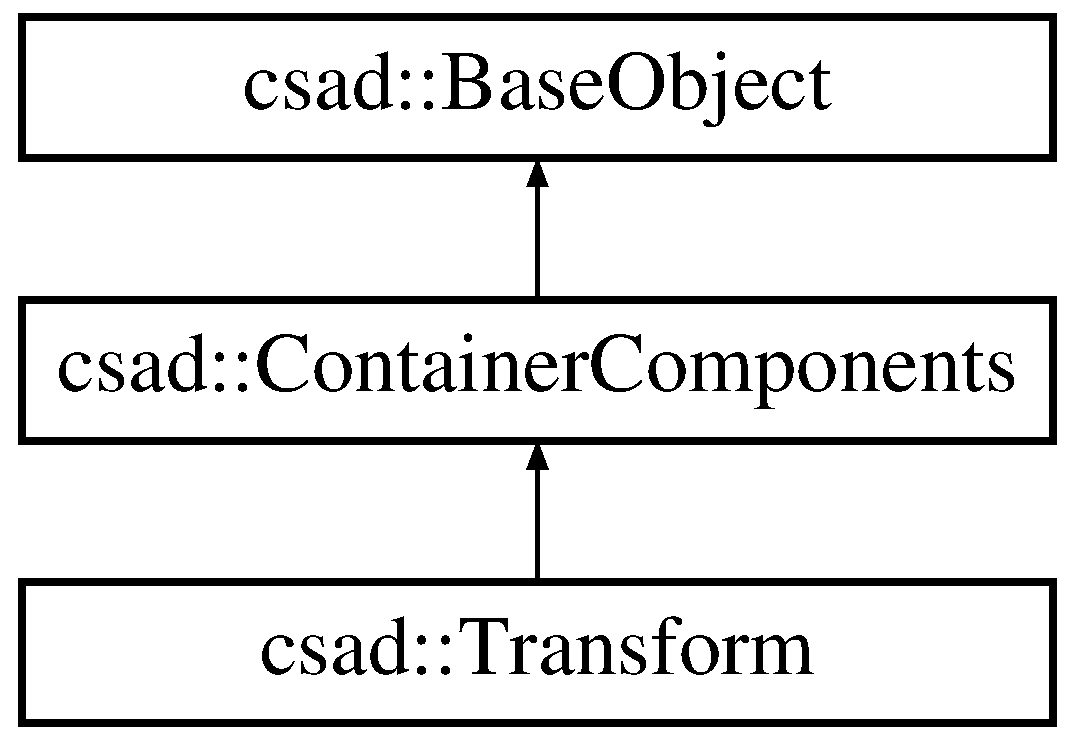
\includegraphics[height=3.000000cm]{classcsad_1_1_transform}
\end{center}
\end{figure}
\subsection*{Public Member Functions}
\begin{DoxyCompactItemize}
\item 
\hypertarget{classcsad_1_1_transform_af9ec56591d43d2e55e7c9ba3587cea14}{virtual void \hyperlink{classcsad_1_1_transform_af9ec56591d43d2e55e7c9ba3587cea14}{add\-Child} (\hyperlink{classcsad_1_1_transform}{Transform} $\ast$)=0}\label{classcsad_1_1_transform_af9ec56591d43d2e55e7c9ba3587cea14}

\begin{DoxyCompactList}\small\item\em insert transform to child list. \end{DoxyCompactList}\item 
\hypertarget{classcsad_1_1_transform_a7fa7d1d5f5ab54cc4574cda8a68fa003}{{\footnotesize template$<$typename T $>$ }\\M\-E\-M\-N\-U\-L\-L \-\_\-\-F\-O\-R\-C\-E\-I\-N\-L\-I\-N\-E T $\ast$ \hyperlink{classcsad_1_1_transform_a7fa7d1d5f5ab54cc4574cda8a68fa003}{add\-Component} ()}\label{classcsad_1_1_transform_a7fa7d1d5f5ab54cc4574cda8a68fa003}

\begin{DoxyCompactList}\small\item\em Adds the component of the specified type in the container if this component already exists, returns available. \end{DoxyCompactList}\item 
virtual \hyperlink{classcsad_1_1_transform}{Transform} $\ast$ \hyperlink{classcsad_1_1_transform_acc5f53fea600a3a528dfd2b92eb941ab}{Child} (int id)=0
\item 
\hypertarget{classcsad_1_1_transform_a63391ebbf1ad110f5f04c3df85eaa4b7}{\-\_\-\-F\-O\-R\-C\-E\-I\-N\-L\-I\-N\-E unsigned int \hyperlink{classcsad_1_1_transform_a63391ebbf1ad110f5f04c3df85eaa4b7}{Child\-Count} ()}\label{classcsad_1_1_transform_a63391ebbf1ad110f5f04c3df85eaa4b7}

\begin{DoxyCompactList}\small\item\em returns number of dependent objects. \end{DoxyCompactList}\item 
\hypertarget{classcsad_1_1_transform_a9655cfd6b41096dcb4fc684d64f68be8}{\hyperlink{classbt_1_1_sort_void_vector}{Transform\-List} \& \hyperlink{classcsad_1_1_transform_a9655cfd6b41096dcb4fc684d64f68be8}{children} ()}\label{classcsad_1_1_transform_a9655cfd6b41096dcb4fc684d64f68be8}

\begin{DoxyCompactList}\small\item\em the list of dependent objects. \end{DoxyCompactList}\item 
\hypertarget{classcsad_1_1_transform_a6451c94d7824dc6698025e3d133eb2e0}{virtual \hyperlink{classcsad_1_1_transform}{Transform} $\ast$ \hyperlink{classcsad_1_1_transform_a6451c94d7824dc6698025e3d133eb2e0}{create\-Transform} (char $\ast$name)=0}\label{classcsad_1_1_transform_a6451c94d7824dc6698025e3d133eb2e0}

\begin{DoxyCompactList}\small\item\em creates a dependent object. \end{DoxyCompactList}\item 
\hypertarget{classcsad_1_1_transform_a01d84357317f0b6e21bcc46e49945766}{virtual void \hyperlink{classcsad_1_1_transform_a01d84357317f0b6e21bcc46e49945766}{delete\-Childs} ()=0}\label{classcsad_1_1_transform_a01d84357317f0b6e21bcc46e49945766}

\begin{DoxyCompactList}\small\item\em delete all childs. \end{DoxyCompactList}\item 
\hypertarget{classcsad_1_1_transform_a2b87024c697a4c9ac79a30359799fd45}{virtual void \hyperlink{classcsad_1_1_transform_a2b87024c697a4c9ac79a30359799fd45}{detach\-Child} (\hyperlink{classcsad_1_1_transform}{Transform} $\ast$child)=0}\label{classcsad_1_1_transform_a2b87024c697a4c9ac79a30359799fd45}

\begin{DoxyCompactList}\small\item\em remove transform from child list. \end{DoxyCompactList}\item 
\hypertarget{classcsad_1_1_transform_a9e830ddc111afbc7c99b30a228601e6c}{\-\_\-\-F\-O\-R\-C\-E\-I\-N\-L\-I\-N\-E \hyperlink{classcsad_1_1_scene}{Scene} $\ast$ \hyperlink{classcsad_1_1_transform_a9e830ddc111afbc7c99b30a228601e6c}{get\-Scene} ()}\label{classcsad_1_1_transform_a9e830ddc111afbc7c99b30a228601e6c}

\begin{DoxyCompactList}\small\item\em returns the scene to which an object belongs. \end{DoxyCompactList}\item 
\hypertarget{classcsad_1_1_transform_a2b0acd6ec11c72f62332ec9b23be784d}{virtual \hyperlink{classcsad_1_1_transform}{Transform} $\ast$ \hyperlink{classcsad_1_1_transform_a2b0acd6ec11c72f62332ec9b23be784d}{get\-Transform} (char $\ast$name)=0}\label{classcsad_1_1_transform_a2b0acd6ec11c72f62332ec9b23be784d}

\begin{DoxyCompactList}\small\item\em restores the dependent object by name. \end{DoxyCompactList}\item 
\hypertarget{classcsad_1_1_transform_ab16040e7ea09b85857c7c8974cb8d234}{\-\_\-\-F\-O\-R\-C\-E\-I\-N\-L\-I\-N\-E \hyperlink{classcsad_1_1_transform}{Transform} $\ast$ \hyperlink{classcsad_1_1_transform_ab16040e7ea09b85857c7c8974cb8d234}{parent} ()}\label{classcsad_1_1_transform_ab16040e7ea09b85857c7c8974cb8d234}

\begin{DoxyCompactList}\small\item\em returns the parent object. \end{DoxyCompactList}\item 
\hypertarget{classcsad_1_1_transform_a9724286b8e4dce45c3e645a1a20fb9bd}{\-\_\-\-F\-O\-R\-C\-E\-I\-N\-L\-I\-N\-E \hyperlink{classbt_1_1vector3d}{vector3d} $\ast$ \hyperlink{classcsad_1_1_transform_a9724286b8e4dce45c3e645a1a20fb9bd}{real\-Position} ()}\label{classcsad_1_1_transform_a9724286b8e4dce45c3e645a1a20fb9bd}

\begin{DoxyCompactList}\small\item\em returns the actual position of the object \end{DoxyCompactList}\item 
\hypertarget{classcsad_1_1_transform_a3e01bf3696fe5e7387ab989e3a462258}{\-\_\-\-F\-O\-R\-C\-E\-I\-N\-L\-I\-N\-E \hyperlink{classbt_1_1quaterniond}{quaterniond} $\ast$ \hyperlink{classcsad_1_1_transform_a3e01bf3696fe5e7387ab989e3a462258}{real\-Rotate} ()}\label{classcsad_1_1_transform_a3e01bf3696fe5e7387ab989e3a462258}

\begin{DoxyCompactList}\small\item\em returns the real razvorot object \end{DoxyCompactList}\item 
\hypertarget{classcsad_1_1_transform_a04118ba35a24790340f4ccb485d574a7}{\-\_\-\-F\-O\-R\-C\-E\-I\-N\-L\-I\-N\-E \hyperlink{classbt_1_1vector3f}{vector3f} $\ast$ \hyperlink{classcsad_1_1_transform_a04118ba35a24790340f4ccb485d574a7}{real\-Scale} ()}\label{classcsad_1_1_transform_a04118ba35a24790340f4ccb485d574a7}

\begin{DoxyCompactList}\small\item\em returns the real scale \end{DoxyCompactList}\item 
virtual void \hyperlink{classcsad_1_1_transform_a5fce29724a5e26c3fab77c2546957f9a}{set\-Child\-Real} (\hyperlink{classcsad_1_1_transform}{Transform} $\ast$transform)=0
\item 
virtual void \hyperlink{classcsad_1_1_transform_a4931301d16d9cd801bdfc14c2b0b9dd7}{set\-Parent\-Real} (\hyperlink{classcsad_1_1_transform}{Transform} $\ast$transform)=0
\item 
virtual \hyperlink{classcsad_1_1_transform}{Transform} \& \hyperlink{classcsad_1_1_transform_a8c0308fb4a1103cb8a263edb3d056346}{set\-Position} (double x, double y, double z)=0
\item 
virtual \hyperlink{classcsad_1_1_transform}{Transform} \& \hyperlink{classcsad_1_1_transform_acae94f7cc01c1624c1b92b23038ff73a}{set\-Position} (\hyperlink{classbt_1_1vector3d}{vector3d} \&pos)=0
\item 
virtual \hyperlink{classcsad_1_1_transform}{Transform} \& \hyperlink{classcsad_1_1_transform_af4dfd9ed7eeb7047080f4d3e7bc09bdb}{set\-Position} (const \hyperlink{classbt_1_1vector3d}{vector3d} \&pos)=0
\item 
virtual \hyperlink{classcsad_1_1_transform}{Transform} \& \hyperlink{classcsad_1_1_transform_af7804a2ba14b15d241049156123bd49f}{set\-Rotate} (const \hyperlink{classbt_1_1quaterniond}{quaterniond} \&\-\_\-rotate)=0
\item 
virtual \hyperlink{classcsad_1_1_transform}{Transform} \& \hyperlink{classcsad_1_1_transform_ab6dec9e170dbbea0fae84ff439546e54}{set\-Scale} (float x, float y, float z)=0
\item 
virtual \hyperlink{classcsad_1_1_transform}{Transform} \& \hyperlink{classcsad_1_1_transform_a068d783bb86fa953143a6fb0b4ef95a1}{set\-Scale} (const \hyperlink{classbt_1_1vector3f}{vector3f} \&\-\_\-scale)=0
\item 
\hypertarget{classcsad_1_1_transform_a4369d7af34c97abebb107af66b2a55c3}{virtual void \hyperlink{classcsad_1_1_transform_a4369d7af34c97abebb107af66b2a55c3}{set\-Selected} (bool)=0}\label{classcsad_1_1_transform_a4369d7af34c97abebb107af66b2a55c3}

\begin{DoxyCompactList}\small\item\em specifies a choice object. \end{DoxyCompactList}\item 
\hypertarget{classcsad_1_1_transform_a7b1ec977c3632a2109677b5d4e891b7b}{virtual void \hyperlink{classcsad_1_1_transform_a7b1ec977c3632a2109677b5d4e891b7b}{set\-Sprite} (bool)=0}\label{classcsad_1_1_transform_a7b1ec977c3632a2109677b5d4e891b7b}

\begin{DoxyCompactList}\small\item\em the reversal of the object relative to the camera. \end{DoxyCompactList}\item 
\hypertarget{classcsad_1_1_transform_a124a674bcb2d3c0147d713d64e90a17c}{virtual void \hyperlink{classcsad_1_1_transform_a124a674bcb2d3c0147d713d64e90a17c}{set\-Visible} (bool)=0}\label{classcsad_1_1_transform_a124a674bcb2d3c0147d713d64e90a17c}

\begin{DoxyCompactList}\small\item\em sets the object visible. \end{DoxyCompactList}\end{DoxyCompactItemize}
\subsection*{Additional Inherited Members}


\subsection{Detailed Description}
\hyperlink{classcsad_1_1_transform}{Transform} -\/ a key element of the environment specifies the position of the object. 

Object allows you to organize position and recalculation of coordinates for building orientation of the object relative to the calculation point. This allows to minimize, and in some cases eliminate, the loss of accuracy.

For description in the configuration\-: \begin{DoxyVerb}  <Scene name="myScene">
    <Transform name="the name of the transform" pos="x y z of position" rot="x y z and angle rotation" scale="x y z of scale">
      ... internal objects or components ...
    </Transform>
  </Scene>
* \end{DoxyVerb}


\begin{DoxySeeAlso}{See Also}
\hyperlink{group__scene}{csad\-: scene} \hyperlink{classcsad_1_1_scene}{Scene} \hyperlink{classcsad_1_1_container_components}{Container\-Components} 
\end{DoxySeeAlso}


\subsection{Member Function Documentation}
\hypertarget{classcsad_1_1_transform_acc5f53fea600a3a528dfd2b92eb941ab}{\index{csad\-::\-Transform@{csad\-::\-Transform}!Child@{Child}}
\index{Child@{Child}!csad::Transform@{csad\-::\-Transform}}
\subsubsection[{Child}]{\setlength{\rightskip}{0pt plus 5cm}virtual {\bf Transform}$\ast$ csad\-::\-Transform\-::\-Child (
\begin{DoxyParamCaption}
\item[{int}]{id}
\end{DoxyParamCaption}
)\hspace{0.3cm}{\ttfamily [pure virtual]}}}\label{classcsad_1_1_transform_acc5f53fea600a3a528dfd2b92eb941ab}
returns child objects by id. 
\begin{DoxyParams}{Parameters}
{\em id} & -\/ is a position object in child list; \\
\hline
\end{DoxyParams}
\hypertarget{classcsad_1_1_transform_a5fce29724a5e26c3fab77c2546957f9a}{\index{csad\-::\-Transform@{csad\-::\-Transform}!set\-Child\-Real@{set\-Child\-Real}}
\index{set\-Child\-Real@{set\-Child\-Real}!csad::Transform@{csad\-::\-Transform}}
\subsubsection[{set\-Child\-Real}]{\setlength{\rightskip}{0pt plus 5cm}virtual void csad\-::\-Transform\-::set\-Child\-Real (
\begin{DoxyParamCaption}
\item[{{\bf Transform} $\ast$}]{transform}
\end{DoxyParamCaption}
)\hspace{0.3cm}{\ttfamily [pure virtual]}}}\label{classcsad_1_1_transform_a5fce29724a5e26c3fab77c2546957f9a}
recalculation of the actual point down the hierarchy of objects 
\begin{DoxyParams}{Parameters}
{\em transform} & -\/ the object on which is made recalculation. \\
\hline
\end{DoxyParams}
\hypertarget{classcsad_1_1_transform_a4931301d16d9cd801bdfc14c2b0b9dd7}{\index{csad\-::\-Transform@{csad\-::\-Transform}!set\-Parent\-Real@{set\-Parent\-Real}}
\index{set\-Parent\-Real@{set\-Parent\-Real}!csad::Transform@{csad\-::\-Transform}}
\subsubsection[{set\-Parent\-Real}]{\setlength{\rightskip}{0pt plus 5cm}virtual void csad\-::\-Transform\-::set\-Parent\-Real (
\begin{DoxyParamCaption}
\item[{{\bf Transform} $\ast$}]{transform}
\end{DoxyParamCaption}
)\hspace{0.3cm}{\ttfamily [pure virtual]}}}\label{classcsad_1_1_transform_a4931301d16d9cd801bdfc14c2b0b9dd7}
recalculation real coordinates up and down the hierarchy of objects 
\begin{DoxyParams}{Parameters}
{\em transform} & -\/ the object on which is made recalculation. \\
\hline
\end{DoxyParams}
\hypertarget{classcsad_1_1_transform_a8c0308fb4a1103cb8a263edb3d056346}{\index{csad\-::\-Transform@{csad\-::\-Transform}!set\-Position@{set\-Position}}
\index{set\-Position@{set\-Position}!csad::Transform@{csad\-::\-Transform}}
\subsubsection[{set\-Position}]{\setlength{\rightskip}{0pt plus 5cm}virtual {\bf Transform}\& csad\-::\-Transform\-::set\-Position (
\begin{DoxyParamCaption}
\item[{double}]{x, }
\item[{double}]{y, }
\item[{double}]{z}
\end{DoxyParamCaption}
)\hspace{0.3cm}{\ttfamily [pure virtual]}}}\label{classcsad_1_1_transform_a8c0308fb4a1103cb8a263edb3d056346}
sets the position of the object 
\begin{DoxyParams}{Parameters}
{\em x,y,z} & -\/ coordinates relative to the coordinate system of the parent object \\
\hline
\end{DoxyParams}
\hypertarget{classcsad_1_1_transform_acae94f7cc01c1624c1b92b23038ff73a}{\index{csad\-::\-Transform@{csad\-::\-Transform}!set\-Position@{set\-Position}}
\index{set\-Position@{set\-Position}!csad::Transform@{csad\-::\-Transform}}
\subsubsection[{set\-Position}]{\setlength{\rightskip}{0pt plus 5cm}virtual {\bf Transform}\& csad\-::\-Transform\-::set\-Position (
\begin{DoxyParamCaption}
\item[{{\bf vector3d} \&}]{pos}
\end{DoxyParamCaption}
)\hspace{0.3cm}{\ttfamily [pure virtual]}}}\label{classcsad_1_1_transform_acae94f7cc01c1624c1b92b23038ff73a}
sets the position of the object 
\begin{DoxyParams}{Parameters}
{\em pos} & -\/ coordinates relative to the coordinate system of the parent object \\
\hline
\end{DoxyParams}
\hypertarget{classcsad_1_1_transform_af4dfd9ed7eeb7047080f4d3e7bc09bdb}{\index{csad\-::\-Transform@{csad\-::\-Transform}!set\-Position@{set\-Position}}
\index{set\-Position@{set\-Position}!csad::Transform@{csad\-::\-Transform}}
\subsubsection[{set\-Position}]{\setlength{\rightskip}{0pt plus 5cm}virtual {\bf Transform}\& csad\-::\-Transform\-::set\-Position (
\begin{DoxyParamCaption}
\item[{const {\bf vector3d} \&}]{pos}
\end{DoxyParamCaption}
)\hspace{0.3cm}{\ttfamily [pure virtual]}}}\label{classcsad_1_1_transform_af4dfd9ed7eeb7047080f4d3e7bc09bdb}
sets the position of the object 
\begin{DoxyParams}{Parameters}
{\em pos} & -\/ coordinates relative to the coordinate system of the parent object \\
\hline
\end{DoxyParams}
\hypertarget{classcsad_1_1_transform_af7804a2ba14b15d241049156123bd49f}{\index{csad\-::\-Transform@{csad\-::\-Transform}!set\-Rotate@{set\-Rotate}}
\index{set\-Rotate@{set\-Rotate}!csad::Transform@{csad\-::\-Transform}}
\subsubsection[{set\-Rotate}]{\setlength{\rightskip}{0pt plus 5cm}virtual {\bf Transform}\& csad\-::\-Transform\-::set\-Rotate (
\begin{DoxyParamCaption}
\item[{const {\bf quaterniond} \&}]{\-\_\-rotate}
\end{DoxyParamCaption}
)\hspace{0.3cm}{\ttfamily [pure virtual]}}}\label{classcsad_1_1_transform_af7804a2ba14b15d241049156123bd49f}
sets the reversal of the object 
\begin{DoxyParams}{Parameters}
{\em \-\_\-rotate} & -\/ quaternion razvorot relation to the position of the parent object \\
\hline
\end{DoxyParams}
\hypertarget{classcsad_1_1_transform_ab6dec9e170dbbea0fae84ff439546e54}{\index{csad\-::\-Transform@{csad\-::\-Transform}!set\-Scale@{set\-Scale}}
\index{set\-Scale@{set\-Scale}!csad::Transform@{csad\-::\-Transform}}
\subsubsection[{set\-Scale}]{\setlength{\rightskip}{0pt plus 5cm}virtual {\bf Transform}\& csad\-::\-Transform\-::set\-Scale (
\begin{DoxyParamCaption}
\item[{float}]{x, }
\item[{float}]{y, }
\item[{float}]{z}
\end{DoxyParamCaption}
)\hspace{0.3cm}{\ttfamily [pure virtual]}}}\label{classcsad_1_1_transform_ab6dec9e170dbbea0fae84ff439546e54}
sets the scale of the object 
\begin{DoxyParams}{Parameters}
{\em x,y,z} & -\/ the scale of the axes relative to the scale of the parent object \\
\hline
\end{DoxyParams}
\hypertarget{classcsad_1_1_transform_a068d783bb86fa953143a6fb0b4ef95a1}{\index{csad\-::\-Transform@{csad\-::\-Transform}!set\-Scale@{set\-Scale}}
\index{set\-Scale@{set\-Scale}!csad::Transform@{csad\-::\-Transform}}
\subsubsection[{set\-Scale}]{\setlength{\rightskip}{0pt plus 5cm}virtual {\bf Transform}\& csad\-::\-Transform\-::set\-Scale (
\begin{DoxyParamCaption}
\item[{const {\bf vector3f} \&}]{\-\_\-scale}
\end{DoxyParamCaption}
)\hspace{0.3cm}{\ttfamily [pure virtual]}}}\label{classcsad_1_1_transform_a068d783bb86fa953143a6fb0b4ef95a1}
sets the scale of the object 
\begin{DoxyParams}{Parameters}
{\em pos} & -\/ the scale relative to the scale of the parent object \\
\hline
\end{DoxyParams}

\hypertarget{classcsad_1_1_v_b_o_mesh}{\section{csad\-:\-:V\-B\-O\-Mesh Class Reference}
\label{classcsad_1_1_v_b_o_mesh}\index{csad\-::\-V\-B\-O\-Mesh@{csad\-::\-V\-B\-O\-Mesh}}
}


\hyperlink{classcsad_1_1_v_b_o_mesh}{V\-B\-O\-Mesh} -\/ class geometry of the device.  


Inheritance diagram for csad\-:\-:V\-B\-O\-Mesh\-:\begin{figure}[H]
\begin{center}
\leavevmode
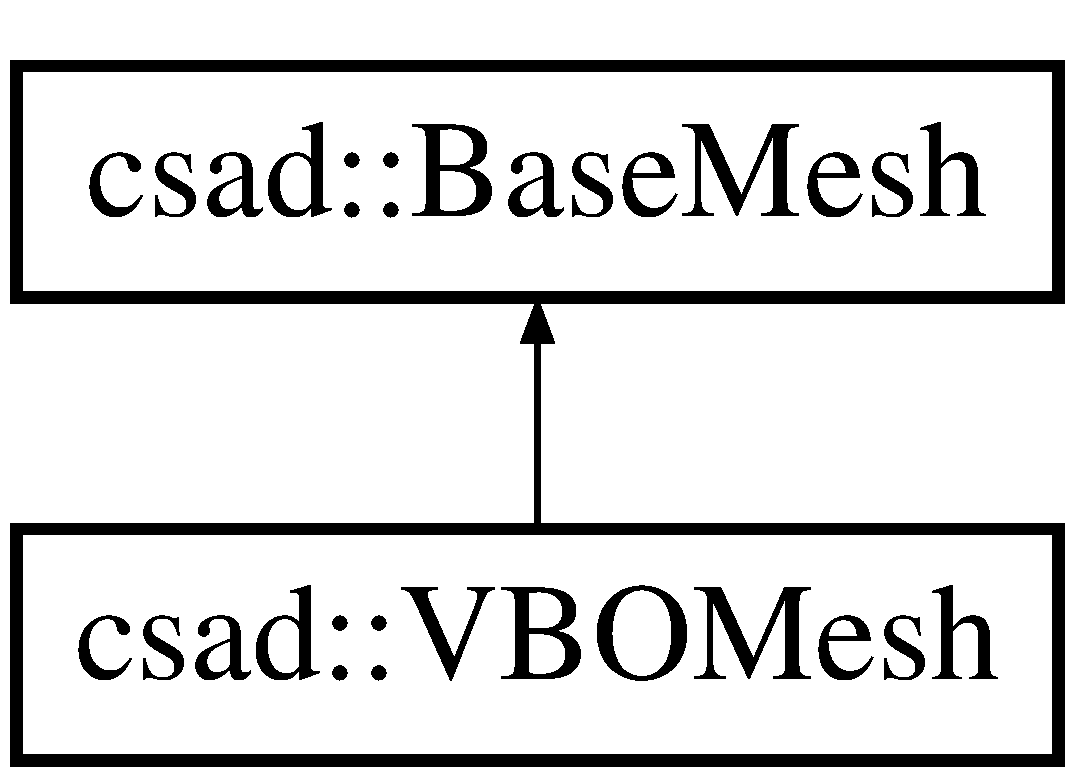
\includegraphics[height=2.000000cm]{classcsad_1_1_v_b_o_mesh}
\end{center}
\end{figure}
\subsection*{Public Attributes}
\begin{DoxyCompactItemize}
\item 
\hypertarget{classcsad_1_1_v_b_o_mesh_af465608edde03a20effa59c302f904b2}{unsigned int \hyperlink{classcsad_1_1_v_b_o_mesh_af465608edde03a20effa59c302f904b2}{elements}}\label{classcsad_1_1_v_b_o_mesh_af465608edde03a20effa59c302f904b2}

\begin{DoxyCompactList}\small\item\em identifier array elements \end{DoxyCompactList}\item 
\hypertarget{classcsad_1_1_v_b_o_mesh_a83c1f273c1431edf40ce3919d6899626}{unsigned int \hyperlink{classcsad_1_1_v_b_o_mesh_a83c1f273c1431edf40ce3919d6899626}{index}}\label{classcsad_1_1_v_b_o_mesh_a83c1f273c1431edf40ce3919d6899626}

\begin{DoxyCompactList}\small\item\em identifier indexes \end{DoxyCompactList}\end{DoxyCompactItemize}


\subsection{Detailed Description}
\hyperlink{classcsad_1_1_v_b_o_mesh}{V\-B\-O\-Mesh} -\/ class geometry of the device. 

Provides support for virtual buffer to store the geometry on the graphics device.

\begin{DoxySeeAlso}{See Also}
\hyperlink{group__scene}{csad\-: scene} 
\end{DoxySeeAlso}

\hypertarget{classcsad_1_1_view_port}{\section{csad\-:\-:View\-Port Class Reference}
\label{classcsad_1_1_view_port}\index{csad\-::\-View\-Port@{csad\-::\-View\-Port}}
}


\hyperlink{classcsad_1_1_view_port}{View\-Port} -\/ rectangular area of the screen where the image is built.  


\subsection*{Public Member Functions}
\begin{DoxyCompactItemize}
\item 
\hypertarget{classcsad_1_1_view_port_a8e7daa8559a2fa9be052f44ba3d3e703}{\-\_\-\-F\-O\-R\-C\-E\-I\-N\-L\-I\-N\-E float \hyperlink{classcsad_1_1_view_port_a8e7daa8559a2fa9be052f44ba3d3e703}{get\-Height} ()}\label{classcsad_1_1_view_port_a8e7daa8559a2fa9be052f44ba3d3e703}

\begin{DoxyCompactList}\small\item\em Returns the height ratio. \end{DoxyCompactList}\item 
\hypertarget{classcsad_1_1_view_port_a0ad927fcbd22508c7bdd613c02c5d53b}{C\-S\-A\-D\-\_\-\-A\-P\-I \hyperlink{classbt_1_1vector4f}{vector4f} \& \hyperlink{classcsad_1_1_view_port_a0ad927fcbd22508c7bdd613c02c5d53b}{get\-Rect} ()}\label{classcsad_1_1_view_port_a0ad927fcbd22508c7bdd613c02c5d53b}

\begin{DoxyCompactList}\small\item\em Returns the coefficients position and size the window display. \end{DoxyCompactList}\item 
\hypertarget{classcsad_1_1_view_port_ac9f6d3c02440a2c9acba861a0573386b}{C\-S\-A\-D\-\_\-\-A\-P\-I \hyperlink{classbt_1_1vector4i}{vector4i} \hyperlink{classcsad_1_1_view_port_ac9f6d3c02440a2c9acba861a0573386b}{get\-Rect} (\hyperlink{classcsad_1_1_gl_context}{Gl\-Context} $\ast$context)}\label{classcsad_1_1_view_port_ac9f6d3c02440a2c9acba861a0573386b}

\begin{DoxyCompactList}\small\item\em Calculates the size of the window in pixels. \end{DoxyCompactList}\item 
\hypertarget{classcsad_1_1_view_port_a23d82391b0590323949d6ff035b24b1d}{C\-S\-A\-D\-\_\-\-A\-P\-I \hyperlink{classbt_1_1vector4i}{vector4i} \hyperlink{classcsad_1_1_view_port_a23d82391b0590323949d6ff035b24b1d}{get\-Rect} (\hyperlink{classcsad_1_1_display}{Display} $\ast$display)}\label{classcsad_1_1_view_port_a23d82391b0590323949d6ff035b24b1d}

\begin{DoxyCompactList}\small\item\em Calculates the size of the window in pixels. \end{DoxyCompactList}\item 
\hypertarget{classcsad_1_1_view_port_a1d81274639278eff0d772a3fcd88c158}{\-\_\-\-F\-O\-R\-C\-E\-I\-N\-L\-I\-N\-E float \hyperlink{classcsad_1_1_view_port_a1d81274639278eff0d772a3fcd88c158}{get\-Width} ()}\label{classcsad_1_1_view_port_a1d81274639278eff0d772a3fcd88c158}

\begin{DoxyCompactList}\small\item\em Returns the width ratio. \end{DoxyCompactList}\item 
\hypertarget{classcsad_1_1_view_port_a8f0a6967461ee52e79244b7620b09a8a}{\-\_\-\-F\-O\-R\-C\-E\-I\-N\-L\-I\-N\-E float \hyperlink{classcsad_1_1_view_port_a8f0a6967461ee52e79244b7620b09a8a}{get\-X} ()}\label{classcsad_1_1_view_port_a8f0a6967461ee52e79244b7620b09a8a}

\begin{DoxyCompactList}\small\item\em returns smashie right from the bottom left corner \end{DoxyCompactList}\item 
\hypertarget{classcsad_1_1_view_port_aee352c063a3c329b71ed3e66433608d6}{\-\_\-\-F\-O\-R\-C\-E\-I\-N\-L\-I\-N\-E float \hyperlink{classcsad_1_1_view_port_aee352c063a3c329b71ed3e66433608d6}{get\-Y} ()}\label{classcsad_1_1_view_port_aee352c063a3c329b71ed3e66433608d6}

\begin{DoxyCompactList}\small\item\em Returns mixing up from the bottom left corner. \end{DoxyCompactList}\item 
\hypertarget{classcsad_1_1_view_port_a756ec12d5be881ab6ce01d686d3d09f5}{C\-S\-A\-D\-\_\-\-A\-P\-I void \hyperlink{classcsad_1_1_view_port_a756ec12d5be881ab6ce01d686d3d09f5}{set\-Full} ()}\label{classcsad_1_1_view_port_a756ec12d5be881ab6ce01d686d3d09f5}

\begin{DoxyCompactList}\small\item\em Sets the display window in the context size. \end{DoxyCompactList}\item 
\hypertarget{classcsad_1_1_view_port_aef7148d13aecabbaab7530fb273c5797}{\-\_\-\-F\-O\-R\-C\-E\-I\-N\-L\-I\-N\-E void \hyperlink{classcsad_1_1_view_port_aef7148d13aecabbaab7530fb273c5797}{set\-Rect} (\hyperlink{classbt_1_1vector4f}{vector4f} \&rect)}\label{classcsad_1_1_view_port_aef7148d13aecabbaab7530fb273c5797}

\begin{DoxyCompactList}\small\item\em Specifies mastasia dimensions region. \end{DoxyCompactList}\end{DoxyCompactItemize}


\subsection{Detailed Description}
\hyperlink{classcsad_1_1_view_port}{View\-Port} -\/ rectangular area of the screen where the image is built. 

\begin{DoxySeeAlso}{See Also}
\hyperlink{group__scene}{csad\-: scene} 
\end{DoxySeeAlso}

\hypertarget{classgen_1_1_geometry_path}{\section{gen\-:\-:Geometry\-Path$<$ T $>$ Class Template Reference}
\label{classgen_1_1_geometry_path}\index{gen\-::\-Geometry\-Path$<$ T $>$@{gen\-::\-Geometry\-Path$<$ T $>$}}
}


\hyperlink{classgen_1_1_geometry_path}{Geometry\-Path} -\/ Список групп.  


\subsection*{Public Member Functions}
\begin{DoxyCompactItemize}
\item 
\hypertarget{classgen_1_1_geometry_path_a829e2cf8226d6e52a4c8c0eff045e546}{\-\_\-\-F\-O\-R\-C\-E\-I\-N\-L\-I\-N\-E void \hyperlink{classgen_1_1_geometry_path_a829e2cf8226d6e52a4c8c0eff045e546}{add\-Vector} (const T \&vec, bool is\-New=false)}\label{classgen_1_1_geometry_path_a829e2cf8226d6e52a4c8c0eff045e546}

\begin{DoxyCompactList}\small\item\em добавить вершину \end{DoxyCompactList}\item 
\hypertarget{classgen_1_1_geometry_path_ace3349bf907447ae9d54b48c187a0ab9}{\-\_\-\-F\-O\-R\-C\-E\-I\-N\-L\-I\-N\-E void \hyperlink{classgen_1_1_geometry_path_ace3349bf907447ae9d54b48c187a0ab9}{clear} ()}\label{classgen_1_1_geometry_path_ace3349bf907447ae9d54b48c187a0ab9}

\begin{DoxyCompactList}\small\item\em очистка \end{DoxyCompactList}\item 
\hypertarget{classgen_1_1_geometry_path_ae68fcefe5338027f8944f76d53d391ba}{\-\_\-\-F\-O\-R\-C\-E\-I\-N\-L\-I\-N\-E unsigned int \hyperlink{classgen_1_1_geometry_path_ae68fcefe5338027f8944f76d53d391ba}{count} ()}\label{classgen_1_1_geometry_path_ae68fcefe5338027f8944f76d53d391ba}

\begin{DoxyCompactList}\small\item\em returns the total number of vertices \end{DoxyCompactList}\item 
\hypertarget{classgen_1_1_geometry_path_a4da13ef48b221e132f6a140ce609cda4}{\-\_\-\-F\-O\-R\-C\-E\-I\-N\-L\-I\-N\-E \hyperlink{classbt_1_1_vector}{List\-Poligon\-Size} \& \hyperlink{classgen_1_1_geometry_path_a4da13ef48b221e132f6a140ce609cda4}{poligon\-Size} ()}\label{classgen_1_1_geometry_path_a4da13ef48b221e132f6a140ce609cda4}

\begin{DoxyCompactList}\small\item\em returns the number of vertices in groups. \end{DoxyCompactList}\item 
\hypertarget{classgen_1_1_geometry_path_ac50a055162b650be01e9f3424270e7d4}{\-\_\-\-F\-O\-R\-C\-E\-I\-N\-L\-I\-N\-E \hyperlink{classbt_1_1_vector}{Vector}$<$ T $>$ \& \hyperlink{classgen_1_1_geometry_path_ac50a055162b650be01e9f3424270e7d4}{vectors} ()}\label{classgen_1_1_geometry_path_ac50a055162b650be01e9f3424270e7d4}

\begin{DoxyCompactList}\small\item\em returns a list of all vertices. \end{DoxyCompactList}\end{DoxyCompactItemize}


\subsection{Detailed Description}
\subsubsection*{template$<$typename T$>$class gen\-::\-Geometry\-Path$<$ T $>$}

\hyperlink{classgen_1_1_geometry_path}{Geometry\-Path} -\/ Список групп. 

\begin{DoxySeeAlso}{See Also}
\hyperlink{group__generator}{gen\-: generator} 
\end{DoxySeeAlso}

\hypertarget{classgen_1_1_modeller_mesh}{\section{gen\-:\-:Modeller\-Mesh Class Reference}
\label{classgen_1_1_modeller_mesh}\index{gen\-::\-Modeller\-Mesh@{gen\-::\-Modeller\-Mesh}}
}


\hyperlink{classgen_1_1_modeller_mesh}{Modeller\-Mesh} -\/ методы моделирования трехмерной полигональной модели.  


\subsection*{Public Member Functions}
\begin{DoxyCompactItemize}
\item 
G\-E\-N\-\_\-\-A\-P\-I void \hyperlink{classgen_1_1_modeller_mesh_a4c845b73d757a4e4054c1a4ae1ea24c6}{add\-Array} (\hyperlink{classbt_1_1_vector}{Vector}$<$ \hyperlink{classbt_1_1vector2i}{vector2i} $>$ $\ast$arr, unsigned int from=0, unsigned int count=0)
\item 
G\-E\-N\-\_\-\-A\-P\-I void \hyperlink{classgen_1_1_modeller_mesh_a84249a4526f804014a165d974b20aec1}{add\-Array} (\hyperlink{classbt_1_1_vector}{Vector}$<$ \hyperlink{classbt_1_1vector2f}{vector2f} $>$ $\ast$arr, unsigned int from=0, unsigned int count=0)
\item 
G\-E\-N\-\_\-\-A\-P\-I void \hyperlink{classgen_1_1_modeller_mesh_a49425074063dc69bbf94db6102d10cd7}{add\-Array} (\hyperlink{classbt_1_1_vector}{Vector}$<$ \hyperlink{classbt_1_1vector3f}{vector3f} $>$ $\ast$arr, unsigned int from=0, unsigned int count=0)
\item 
\hypertarget{classgen_1_1_modeller_mesh_a9ebfc30ad05b4eb96b0987f1ec771a2d}{G\-E\-N\-\_\-\-A\-P\-I void \hyperlink{classgen_1_1_modeller_mesh_a9ebfc30ad05b4eb96b0987f1ec771a2d}{add\-By\-Tess} (void $\ast$tess)}\label{classgen_1_1_modeller_mesh_a9ebfc30ad05b4eb96b0987f1ec771a2d}

\begin{DoxyCompactList}\small\item\em Добавляет результат тесселяции \end{DoxyCompactList}\item 
\hypertarget{classgen_1_1_modeller_mesh_a68859cdf93897bf3b7a925e7ad746386}{G\-E\-N\-\_\-\-A\-P\-I void \hyperlink{classgen_1_1_modeller_mesh_a68859cdf93897bf3b7a925e7ad746386}{add\-Rotation} (\hyperlink{classbt_1_1quaterniond}{quaterniond} $\ast$rot)}\label{classgen_1_1_modeller_mesh_a68859cdf93897bf3b7a925e7ad746386}

\begin{DoxyCompactList}\small\item\em Добавляет разворок к матрице трансформации. \end{DoxyCompactList}\item 
\hypertarget{classgen_1_1_modeller_mesh_abb4141f0cd7f98804b36a888fa71595c}{G\-E\-N\-\_\-\-A\-P\-I void \hyperlink{classgen_1_1_modeller_mesh_abb4141f0cd7f98804b36a888fa71595c}{add\-Scale} (\hyperlink{classbt_1_1vector3f}{vector3f} $\ast$scale)}\label{classgen_1_1_modeller_mesh_abb4141f0cd7f98804b36a888fa71595c}

\begin{DoxyCompactList}\small\item\em Добавляет масштаб к матрице трансформации. \end{DoxyCompactList}\item 
\hypertarget{classgen_1_1_modeller_mesh_a5c922811fe3de16a4271eb2fe3ae7307}{G\-E\-N\-\_\-\-A\-P\-I void \hyperlink{classgen_1_1_modeller_mesh_a5c922811fe3de16a4271eb2fe3ae7307}{add\-Translate} (\hyperlink{classbt_1_1vector3d}{vector3d} $\ast$pos)}\label{classgen_1_1_modeller_mesh_a5c922811fe3de16a4271eb2fe3ae7307}

\begin{DoxyCompactList}\small\item\em Добавляет смещение к матрице трансформации. \end{DoxyCompactList}\item 
\hypertarget{classgen_1_1_modeller_mesh_a7e58ea4100de31965e707c65045b1684}{G\-E\-N\-\_\-\-A\-P\-I void \hyperlink{classgen_1_1_modeller_mesh_a7e58ea4100de31965e707c65045b1684}{add\-Translate} (double x, double y, double z)}\label{classgen_1_1_modeller_mesh_a7e58ea4100de31965e707c65045b1684}

\begin{DoxyCompactList}\small\item\em Добавляет смещение к матрице трансформации. \end{DoxyCompactList}\item 
G\-E\-N\-\_\-\-A\-P\-I void \hyperlink{classgen_1_1_modeller_mesh_a5a706b85444623b8ec0e82f8e84492be}{circle} (float radius, unsigned int cells, float start=0, float end=0)
\item 
\hypertarget{classgen_1_1_modeller_mesh_a735911c67efd79e24f1eaa04e1a320e9}{G\-E\-N\-\_\-\-A\-P\-I void \hyperlink{classgen_1_1_modeller_mesh_a735911c67efd79e24f1eaa04e1a320e9}{copy\-Index} (\hyperlink{classcsad_1_1_mesh}{Mesh} $\ast$mesh, unsigned int at, unsigned int from, unsigned int count, int off)}\label{classgen_1_1_modeller_mesh_a735911c67efd79e24f1eaa04e1a320e9}

\begin{DoxyCompactList}\small\item\em Внутреннее копирование индексов \end{DoxyCompactList}\item 
\hypertarget{classgen_1_1_modeller_mesh_aeace268c2b1f26dc42231577aa77ee8a}{G\-E\-N\-\_\-\-A\-P\-I void \hyperlink{classgen_1_1_modeller_mesh_aeace268c2b1f26dc42231577aa77ee8a}{copy\-Vertex} (\hyperlink{classcsad_1_1_mesh}{Mesh} $\ast$mesh, unsigned int at, unsigned int from, unsigned int count)}\label{classgen_1_1_modeller_mesh_aeace268c2b1f26dc42231577aa77ee8a}

\begin{DoxyCompactList}\small\item\em Внутреннее копирование вершин \end{DoxyCompactList}\item 
G\-E\-N\-\_\-\-A\-P\-I void \hyperlink{classgen_1_1_modeller_mesh_a35d7e7c91979cd64f6fa1b7146e6a724}{fill} (Geometry\-Path2\-F $\ast$path, float bsmooth=0)
\item 
G\-E\-N\-\_\-\-A\-P\-I void \hyperlink{classgen_1_1_modeller_mesh_a18758d6962ed3b34eaf9c8fabc2ef371}{quad} (float width, float height, float bsmooth=0)
\item 
\hypertarget{classgen_1_1_modeller_mesh_a688df921a9895224753ec4a7fd095ae7}{G\-E\-N\-\_\-\-A\-P\-I void \hyperlink{classgen_1_1_modeller_mesh_a688df921a9895224753ec4a7fd095ae7}{reset\-Matrix} ()}\label{classgen_1_1_modeller_mesh_a688df921a9895224753ec4a7fd095ae7}

\begin{DoxyCompactList}\small\item\em устанавливает единичную матрицу трансформации. \end{DoxyCompactList}\item 
\hypertarget{classgen_1_1_modeller_mesh_a67054bfc7fd92c96727b8e63daf2e613}{G\-E\-N\-\_\-\-A\-P\-I void \hyperlink{classgen_1_1_modeller_mesh_a67054bfc7fd92c96727b8e63daf2e613}{Rotate} (\hyperlink{classbt_1_1vector3d}{vector3d} $\ast$rot)}\label{classgen_1_1_modeller_mesh_a67054bfc7fd92c96727b8e63daf2e613}

\begin{DoxyCompactList}\small\item\em разварачивает имеющиеся вершины \end{DoxyCompactList}\item 
\hypertarget{classgen_1_1_modeller_mesh_ada4d30f9ddb5f163ad4f9fb2c3f7846d}{G\-E\-N\-\_\-\-A\-P\-I void \hyperlink{classgen_1_1_modeller_mesh_ada4d30f9ddb5f163ad4f9fb2c3f7846d}{Scale} (\hyperlink{classbt_1_1vector3f}{vector3f} $\ast$scale)}\label{classgen_1_1_modeller_mesh_ada4d30f9ddb5f163ad4f9fb2c3f7846d}

\begin{DoxyCompactList}\small\item\em масштабирует имеющиеся вершины \end{DoxyCompactList}\item 
\hypertarget{classgen_1_1_modeller_mesh_ae32222a9066a9ecb78c07cf9b9639bfd}{G\-E\-N\-\_\-\-A\-P\-I void \hyperlink{classgen_1_1_modeller_mesh_ae32222a9066a9ecb78c07cf9b9639bfd}{set\-Color} (unsigned int color)}\label{classgen_1_1_modeller_mesh_ae32222a9066a9ecb78c07cf9b9639bfd}

\begin{DoxyCompactList}\small\item\em Задает модификатор цвета вершин \end{DoxyCompactList}\item 
\hypertarget{classgen_1_1_modeller_mesh_ac7df9d964d1c5bb6058957086ee503f7}{G\-E\-N\-\_\-\-A\-P\-I void \hyperlink{classgen_1_1_modeller_mesh_ac7df9d964d1c5bb6058957086ee503f7}{set\-Color} (\hyperlink{classbt_1_1vector4f}{vector4f} $\ast$color)}\label{classgen_1_1_modeller_mesh_ac7df9d964d1c5bb6058957086ee503f7}

\begin{DoxyCompactList}\small\item\em Задает модификатор цвета вершин \end{DoxyCompactList}\item 
\hypertarget{classgen_1_1_modeller_mesh_a6e45dcb1c341f4c4eef7fc52a8e58a30}{G\-E\-N\-\_\-\-A\-P\-I void \hyperlink{classgen_1_1_modeller_mesh_a6e45dcb1c341f4c4eef7fc52a8e58a30}{set\-Color} (float b, float g, float r, float a)}\label{classgen_1_1_modeller_mesh_a6e45dcb1c341f4c4eef7fc52a8e58a30}

\begin{DoxyCompactList}\small\item\em Задает модификатор цвета вершин \end{DoxyCompactList}\item 
G\-E\-N\-\_\-\-A\-P\-I void \hyperlink{classgen_1_1_modeller_mesh_a5b960ddde71d17dd8b8b60666cf7ab13}{set\-Mesh} (\hyperlink{classcsad_1_1_mesh}{Mesh} $\ast$mesh)
\item 
G\-E\-N\-\_\-\-A\-P\-I void \hyperlink{classgen_1_1_modeller_mesh_ac333825cc70c6c8f218e218864321f3b}{set\-Mode} (unsigned int mode)
\item 
\hypertarget{classgen_1_1_modeller_mesh_a53a5c8fa04ad6ff83e97f80b1cc0d098}{G\-E\-N\-\_\-\-A\-P\-I void \hyperlink{classgen_1_1_modeller_mesh_a53a5c8fa04ad6ff83e97f80b1cc0d098}{sphere} (float radius, unsigned int wcells, unsigned int hcells)}\label{classgen_1_1_modeller_mesh_a53a5c8fa04ad6ff83e97f80b1cc0d098}

\begin{DoxyCompactList}\small\item\em Моделирует сферу. \end{DoxyCompactList}\item 
G\-E\-N\-\_\-\-A\-P\-I void \hyperlink{classgen_1_1_modeller_mesh_a9bd2a64f71389863d5ec68aebd846715}{stroked\-Circle} (float radius, float width, unsigned int cells, float start=0.\-0f, float end=0.\-0f, float bsmooth=0)
\item 
G\-E\-N\-\_\-\-A\-P\-I void \hyperlink{classgen_1_1_modeller_mesh_a27bee288d0e04f12097aa545074725ee}{stroker} (Geometry\-Path2\-F $\ast$path, float width, float offset)
\item 
\hypertarget{classgen_1_1_modeller_mesh_a33580546f756ef1ffce569418adf387d}{G\-E\-N\-\_\-\-A\-P\-I void \hyperlink{classgen_1_1_modeller_mesh_a33580546f756ef1ffce569418adf387d}{text\-Extrude} (char $\ast$text, \hyperlink{classcsad_1_1_text_style}{Text\-Style} $\ast$style, float z, float extrude=0)}\label{classgen_1_1_modeller_mesh_a33580546f756ef1ffce569418adf387d}

\begin{DoxyCompactList}\small\item\em Вытянутый объемный текст. \end{DoxyCompactList}\item 
\hypertarget{classgen_1_1_modeller_mesh_a550b2136bd21d66b821832d6483b8a79}{G\-E\-N\-\_\-\-A\-P\-I void \hyperlink{classgen_1_1_modeller_mesh_a550b2136bd21d66b821832d6483b8a79}{text\-Flat} (char $\ast$text, \hyperlink{classcsad_1_1_text_style}{Text\-Style} $\ast$style, float z, float bsmooth=0)}\label{classgen_1_1_modeller_mesh_a550b2136bd21d66b821832d6483b8a79}

\begin{DoxyCompactList}\small\item\em Плоский текст. \end{DoxyCompactList}\item 
\hypertarget{classgen_1_1_modeller_mesh_ae80ac72c254d62cad0b54c3038fd449a}{G\-E\-N\-\_\-\-A\-P\-I void \hyperlink{classgen_1_1_modeller_mesh_ae80ac72c254d62cad0b54c3038fd449a}{text\-Texture} (char $\ast$text, \hyperlink{classcsad_1_1_text_style}{Text\-Style} $\ast$style, float z)}\label{classgen_1_1_modeller_mesh_ae80ac72c254d62cad0b54c3038fd449a}

\begin{DoxyCompactList}\small\item\em Текстурный текст. \end{DoxyCompactList}\item 
G\-E\-N\-\_\-\-A\-P\-I void \hyperlink{classgen_1_1_modeller_mesh_a84d7b5bdc92eea09ddc349934c34cf48}{Transform} (unsigned int from, unsigned int count)
\item 
\hypertarget{classgen_1_1_modeller_mesh_a8b8367bb554e0d608041ee3b29df87bd}{G\-E\-N\-\_\-\-A\-P\-I void \hyperlink{classgen_1_1_modeller_mesh_a8b8367bb554e0d608041ee3b29df87bd}{Translate} (\hyperlink{classbt_1_1vector3d}{vector3d} $\ast$pos)}\label{classgen_1_1_modeller_mesh_a8b8367bb554e0d608041ee3b29df87bd}

\begin{DoxyCompactList}\small\item\em смещает имеющиеся вершины \end{DoxyCompactList}\item 
\hypertarget{classgen_1_1_modeller_mesh_ab385e4d790caf0d2d75abe509414a282}{G\-E\-N\-\_\-\-A\-P\-I void \hyperlink{classgen_1_1_modeller_mesh_ab385e4d790caf0d2d75abe509414a282}{T\-R\-S} (\hyperlink{classbt_1_1vector3d}{vector3d} $\ast$pos, \hyperlink{classbt_1_1quaterniond}{quaterniond} $\ast$rot, \hyperlink{classbt_1_1vector3f}{vector3f} $\ast$scale)}\label{classgen_1_1_modeller_mesh_ab385e4d790caf0d2d75abe509414a282}

\begin{DoxyCompactList}\small\item\em Задает матрицу трансформации по смещению развороту и масштабу. \end{DoxyCompactList}\end{DoxyCompactItemize}


\subsection{Detailed Description}
\hyperlink{classgen_1_1_modeller_mesh}{Modeller\-Mesh} -\/ методы моделирования трехмерной полигональной модели. 

\begin{DoxySeeAlso}{See Also}
\hyperlink{group__generator}{gen\-: generator} 
\end{DoxySeeAlso}


\subsection{Member Function Documentation}
\hypertarget{classgen_1_1_modeller_mesh_a4c845b73d757a4e4054c1a4ae1ea24c6}{\index{gen\-::\-Modeller\-Mesh@{gen\-::\-Modeller\-Mesh}!add\-Array@{add\-Array}}
\index{add\-Array@{add\-Array}!gen::ModellerMesh@{gen\-::\-Modeller\-Mesh}}
\subsubsection[{add\-Array}]{\setlength{\rightskip}{0pt plus 5cm}G\-E\-N\-\_\-\-A\-P\-I void gen\-::\-Modeller\-Mesh\-::add\-Array (
\begin{DoxyParamCaption}
\item[{{\bf Vector}$<$ {\bf vector2i} $>$ $\ast$}]{arr, }
\item[{unsigned int}]{from = {\ttfamily 0}, }
\item[{unsigned int}]{count = {\ttfamily 0}}
\end{DoxyParamCaption}
)}}\label{classgen_1_1_modeller_mesh_a4c845b73d757a4e4054c1a4ae1ea24c6}
Добавляет массив вершин 
\begin{DoxyParams}{Parameters}
{\em arr} & -\/ масивв вершин. \\
\hline
{\em from} & -\/ первый элемент массива. \\
\hline
{\em count} & -\/ количество добвляемых элементов. \\
\hline
\end{DoxyParams}
\hypertarget{classgen_1_1_modeller_mesh_a84249a4526f804014a165d974b20aec1}{\index{gen\-::\-Modeller\-Mesh@{gen\-::\-Modeller\-Mesh}!add\-Array@{add\-Array}}
\index{add\-Array@{add\-Array}!gen::ModellerMesh@{gen\-::\-Modeller\-Mesh}}
\subsubsection[{add\-Array}]{\setlength{\rightskip}{0pt plus 5cm}G\-E\-N\-\_\-\-A\-P\-I void gen\-::\-Modeller\-Mesh\-::add\-Array (
\begin{DoxyParamCaption}
\item[{{\bf Vector}$<$ {\bf vector2f} $>$ $\ast$}]{arr, }
\item[{unsigned int}]{from = {\ttfamily 0}, }
\item[{unsigned int}]{count = {\ttfamily 0}}
\end{DoxyParamCaption}
)}}\label{classgen_1_1_modeller_mesh_a84249a4526f804014a165d974b20aec1}
Добавляет массив вершин 
\begin{DoxyParams}{Parameters}
{\em arr} & -\/ масивв вершин. \\
\hline
{\em from} & -\/ первый элемент массива. \\
\hline
{\em count} & -\/ количество добвляемых элементов. \\
\hline
\end{DoxyParams}
\hypertarget{classgen_1_1_modeller_mesh_a49425074063dc69bbf94db6102d10cd7}{\index{gen\-::\-Modeller\-Mesh@{gen\-::\-Modeller\-Mesh}!add\-Array@{add\-Array}}
\index{add\-Array@{add\-Array}!gen::ModellerMesh@{gen\-::\-Modeller\-Mesh}}
\subsubsection[{add\-Array}]{\setlength{\rightskip}{0pt plus 5cm}G\-E\-N\-\_\-\-A\-P\-I void gen\-::\-Modeller\-Mesh\-::add\-Array (
\begin{DoxyParamCaption}
\item[{{\bf Vector}$<$ {\bf vector3f} $>$ $\ast$}]{arr, }
\item[{unsigned int}]{from = {\ttfamily 0}, }
\item[{unsigned int}]{count = {\ttfamily 0}}
\end{DoxyParamCaption}
)}}\label{classgen_1_1_modeller_mesh_a49425074063dc69bbf94db6102d10cd7}
Добавляет массив вершин 
\begin{DoxyParams}{Parameters}
{\em arr} & -\/ масивв вершин. \\
\hline
{\em from} & -\/ первый элемент массива. \\
\hline
{\em count} & -\/ количество добвляемых элементов. \\
\hline
\end{DoxyParams}
\hypertarget{classgen_1_1_modeller_mesh_a5a706b85444623b8ec0e82f8e84492be}{\index{gen\-::\-Modeller\-Mesh@{gen\-::\-Modeller\-Mesh}!circle@{circle}}
\index{circle@{circle}!gen::ModellerMesh@{gen\-::\-Modeller\-Mesh}}
\subsubsection[{circle}]{\setlength{\rightskip}{0pt plus 5cm}G\-E\-N\-\_\-\-A\-P\-I void gen\-::\-Modeller\-Mesh\-::circle (
\begin{DoxyParamCaption}
\item[{float}]{radius, }
\item[{unsigned int}]{cells, }
\item[{float}]{start = {\ttfamily 0}, }
\item[{float}]{end = {\ttfamily 0}}
\end{DoxyParamCaption}
)}}\label{classgen_1_1_modeller_mesh_a5a706b85444623b8ec0e82f8e84492be}
Моделирует круг или секцию круга. 
\begin{DoxyParams}{Parameters}
{\em radius} & -\/ радиус. \\
\hline
{\em cells} & -\/ количество шагов по окружности. \\
\hline
{\em start} & -\/ начальный граус. \\
\hline
{\em end} & -\/ конечный граус. \\
\hline
\end{DoxyParams}
\hypertarget{classgen_1_1_modeller_mesh_a35d7e7c91979cd64f6fa1b7146e6a724}{\index{gen\-::\-Modeller\-Mesh@{gen\-::\-Modeller\-Mesh}!fill@{fill}}
\index{fill@{fill}!gen::ModellerMesh@{gen\-::\-Modeller\-Mesh}}
\subsubsection[{fill}]{\setlength{\rightskip}{0pt plus 5cm}G\-E\-N\-\_\-\-A\-P\-I void gen\-::\-Modeller\-Mesh\-::fill (
\begin{DoxyParamCaption}
\item[{Geometry\-Path2\-F $\ast$}]{path, }
\item[{float}]{bsmooth = {\ttfamily 0}}
\end{DoxyParamCaption}
)}}\label{classgen_1_1_modeller_mesh_a35d7e7c91979cd64f6fa1b7146e6a724}
Заливка по форме. 
\begin{DoxyParams}{Parameters}
{\em path} & -\/ форма заливки. \\
\hline
{\em bsmooth} & -\/ размер обводки для сглаживания (antialiasing). \\
\hline
\end{DoxyParams}
\hypertarget{classgen_1_1_modeller_mesh_a18758d6962ed3b34eaf9c8fabc2ef371}{\index{gen\-::\-Modeller\-Mesh@{gen\-::\-Modeller\-Mesh}!quad@{quad}}
\index{quad@{quad}!gen::ModellerMesh@{gen\-::\-Modeller\-Mesh}}
\subsubsection[{quad}]{\setlength{\rightskip}{0pt plus 5cm}G\-E\-N\-\_\-\-A\-P\-I void gen\-::\-Modeller\-Mesh\-::quad (
\begin{DoxyParamCaption}
\item[{float}]{width, }
\item[{float}]{height, }
\item[{float}]{bsmooth = {\ttfamily 0}}
\end{DoxyParamCaption}
)}}\label{classgen_1_1_modeller_mesh_a18758d6962ed3b34eaf9c8fabc2ef371}
Моделирует квадрат. 
\begin{DoxyParams}{Parameters}
{\em width} & -\/ ширина. \\
\hline
{\em height} & -\/ высота. \\
\hline
{\em bsmooth} & -\/ размер обводки для сглаживания (antialiasing). \\
\hline
\end{DoxyParams}
\hypertarget{classgen_1_1_modeller_mesh_a5b960ddde71d17dd8b8b60666cf7ab13}{\index{gen\-::\-Modeller\-Mesh@{gen\-::\-Modeller\-Mesh}!set\-Mesh@{set\-Mesh}}
\index{set\-Mesh@{set\-Mesh}!gen::ModellerMesh@{gen\-::\-Modeller\-Mesh}}
\subsubsection[{set\-Mesh}]{\setlength{\rightskip}{0pt plus 5cm}G\-E\-N\-\_\-\-A\-P\-I void gen\-::\-Modeller\-Mesh\-::set\-Mesh (
\begin{DoxyParamCaption}
\item[{{\bf Mesh} $\ast$}]{mesh}
\end{DoxyParamCaption}
)}}\label{classgen_1_1_modeller_mesh_a5b960ddde71d17dd8b8b60666cf7ab13}
Добавляет массив вершин 
\begin{DoxyParams}{Parameters}
{\em mesh} & -\/ контейнер модели. \\
\hline
\end{DoxyParams}
\hypertarget{classgen_1_1_modeller_mesh_ac333825cc70c6c8f218e218864321f3b}{\index{gen\-::\-Modeller\-Mesh@{gen\-::\-Modeller\-Mesh}!set\-Mode@{set\-Mode}}
\index{set\-Mode@{set\-Mode}!gen::ModellerMesh@{gen\-::\-Modeller\-Mesh}}
\subsubsection[{set\-Mode}]{\setlength{\rightskip}{0pt plus 5cm}G\-E\-N\-\_\-\-A\-P\-I void gen\-::\-Modeller\-Mesh\-::set\-Mode (
\begin{DoxyParamCaption}
\item[{unsigned int}]{mode}
\end{DoxyParamCaption}
)}}\label{classgen_1_1_modeller_mesh_ac333825cc70c6c8f218e218864321f3b}
Задает режим смешивания 
\begin{DoxyParams}{Parameters}
{\em mode} & -\/ режим. \\
\hline
\end{DoxyParams}
\hypertarget{classgen_1_1_modeller_mesh_a9bd2a64f71389863d5ec68aebd846715}{\index{gen\-::\-Modeller\-Mesh@{gen\-::\-Modeller\-Mesh}!stroked\-Circle@{stroked\-Circle}}
\index{stroked\-Circle@{stroked\-Circle}!gen::ModellerMesh@{gen\-::\-Modeller\-Mesh}}
\subsubsection[{stroked\-Circle}]{\setlength{\rightskip}{0pt plus 5cm}G\-E\-N\-\_\-\-A\-P\-I void gen\-::\-Modeller\-Mesh\-::stroked\-Circle (
\begin{DoxyParamCaption}
\item[{float}]{radius, }
\item[{float}]{width, }
\item[{unsigned int}]{cells, }
\item[{float}]{start = {\ttfamily 0.0f}, }
\item[{float}]{end = {\ttfamily 0.0f}, }
\item[{float}]{bsmooth = {\ttfamily 0}}
\end{DoxyParamCaption}
)}}\label{classgen_1_1_modeller_mesh_a9bd2a64f71389863d5ec68aebd846715}
Моделирует обводку круга или отрезок окружности. 
\begin{DoxyParams}{Parameters}
{\em radius} & -\/ радиус. \\
\hline
{\em width} & -\/ ширина обводки. \\
\hline
{\em cells} & -\/ количество шагов по окружности. \\
\hline
{\em start} & -\/ начальный граус. \\
\hline
{\em end} & -\/ конечный граус. \\
\hline
{\em bsmooth} & -\/ размер обводки для сглаживания (antialiasing). \\
\hline
\end{DoxyParams}
\hypertarget{classgen_1_1_modeller_mesh_a27bee288d0e04f12097aa545074725ee}{\index{gen\-::\-Modeller\-Mesh@{gen\-::\-Modeller\-Mesh}!stroker@{stroker}}
\index{stroker@{stroker}!gen::ModellerMesh@{gen\-::\-Modeller\-Mesh}}
\subsubsection[{stroker}]{\setlength{\rightskip}{0pt plus 5cm}G\-E\-N\-\_\-\-A\-P\-I void gen\-::\-Modeller\-Mesh\-::stroker (
\begin{DoxyParamCaption}
\item[{Geometry\-Path2\-F $\ast$}]{path, }
\item[{float}]{width, }
\item[{float}]{offset}
\end{DoxyParamCaption}
)}}\label{classgen_1_1_modeller_mesh_a27bee288d0e04f12097aa545074725ee}
Моделирует линию заданной толщины согласно пути. 
\begin{DoxyParams}{Parameters}
{\em path} & -\/ путь. \\
\hline
{\em width} & -\/ толщина линии. \\
\hline
{\em offset} & -\/ смещение линии от центра. \\
\hline
\end{DoxyParams}
\hypertarget{classgen_1_1_modeller_mesh_a84d7b5bdc92eea09ddc349934c34cf48}{\index{gen\-::\-Modeller\-Mesh@{gen\-::\-Modeller\-Mesh}!Transform@{Transform}}
\index{Transform@{Transform}!gen::ModellerMesh@{gen\-::\-Modeller\-Mesh}}
\subsubsection[{Transform}]{\setlength{\rightskip}{0pt plus 5cm}G\-E\-N\-\_\-\-A\-P\-I void gen\-::\-Modeller\-Mesh\-::\-Transform (
\begin{DoxyParamCaption}
\item[{unsigned int}]{from, }
\item[{unsigned int}]{count}
\end{DoxyParamCaption}
)}}\label{classgen_1_1_modeller_mesh_a84d7b5bdc92eea09ddc349934c34cf48}
трансформирует вершины согласно матрице трансформации. 
\begin{DoxyParams}{Parameters}
{\em from} & -\/ первая вершина. \\
\hline
{\em from} & -\/ количество модифицируемых вершин. \\
\hline
\end{DoxyParams}

\hypertarget{classgen_1_1_modeller_raster}{\section{gen\-:\-:Modeller\-Raster Class Reference}
\label{classgen_1_1_modeller_raster}\index{gen\-::\-Modeller\-Raster@{gen\-::\-Modeller\-Raster}}
}


\hyperlink{classgen_1_1_modeller_raster}{Modeller\-Raster} -\/ методы моделирования изображения.  


\subsection*{Public Member Functions}
\begin{DoxyCompactItemize}
\item 
\hypertarget{classgen_1_1_modeller_raster_aee7897cf040faa7d32d20d2451751c1e}{G\-E\-N\-\_\-\-A\-P\-I void \hyperlink{classgen_1_1_modeller_raster_aee7897cf040faa7d32d20d2451751c1e}{rastertext} (\-\_\-int32 x, \-\_\-int32 y, \-\_\-int32 color, char $\ast$str)}\label{classgen_1_1_modeller_raster_aee7897cf040faa7d32d20d2451751c1e}

\begin{DoxyCompactList}\small\item\em Растеризует текст в цветовую матрицу \end{DoxyCompactList}\item 
\hypertarget{classgen_1_1_modeller_raster_af4ea4623ec7e3742c69011d4a7856f49}{G\-E\-N\-\_\-\-A\-P\-I void \hyperlink{classgen_1_1_modeller_raster_af4ea4623ec7e3742c69011d4a7856f49}{set\-Font} (\hyperlink{classcsad_1_1_font}{csad\-::\-Font} $\ast$font)}\label{classgen_1_1_modeller_raster_af4ea4623ec7e3742c69011d4a7856f49}

\begin{DoxyCompactList}\small\item\em Задает шрифт \end{DoxyCompactList}\item 
\hypertarget{classgen_1_1_modeller_raster_ab5641d45191594225c5581da065c6297}{G\-E\-N\-\_\-\-A\-P\-I void \hyperlink{classgen_1_1_modeller_raster_ab5641d45191594225c5581da065c6297}{set\-Mode} (\-\_\-int32 mode)}\label{classgen_1_1_modeller_raster_ab5641d45191594225c5581da065c6297}

\begin{DoxyCompactList}\small\item\em Задает режим смешивания \end{DoxyCompactList}\item 
\hypertarget{classgen_1_1_modeller_raster_adad120258b87bfdc6678cfad986d6ad9}{G\-E\-N\-\_\-\-A\-P\-I void \hyperlink{classgen_1_1_modeller_raster_adad120258b87bfdc6678cfad986d6ad9}{set\-Raster} (\hyperlink{struct_raster}{Raster} $\ast$raster)}\label{classgen_1_1_modeller_raster_adad120258b87bfdc6678cfad986d6ad9}

\begin{DoxyCompactList}\small\item\em Задает рабочий растр \end{DoxyCompactList}\end{DoxyCompactItemize}
\subsection*{Static Public Member Functions}
\begin{DoxyCompactItemize}
\item 
\hypertarget{classgen_1_1_modeller_raster_a0c18c0642f4c84094d8cd6c0afed975e}{static \-\_\-\-F\-O\-R\-C\-E\-I\-N\-L\-I\-N\-E void \hyperlink{classgen_1_1_modeller_raster_a0c18c0642f4c84094d8cd6c0afed975e}{mix} (\hyperlink{struct_raster}{Raster} $\ast$rastera, \hyperlink{struct_raster}{Raster} $\ast$rasterb, \-\_\-int32 x, \-\_\-int32 y, \-\_\-int32 fill)}\label{classgen_1_1_modeller_raster_a0c18c0642f4c84094d8cd6c0afed975e}

\begin{DoxyCompactList}\small\item\em Смешивает цветовые матрицы \end{DoxyCompactList}\item 
\hypertarget{classgen_1_1_modeller_raster_a1ef12ff68a05743b6182d316028bf375}{static G\-E\-N\-\_\-\-A\-P\-I void \hyperlink{classgen_1_1_modeller_raster_a1ef12ff68a05743b6182d316028bf375}{revers} (void $\ast$data, \-\_\-int32 width\-Bpp, \-\_\-int32 height)}\label{classgen_1_1_modeller_raster_a1ef12ff68a05743b6182d316028bf375}

\begin{DoxyCompactList}\small\item\em переворачивает по вертикали. \end{DoxyCompactList}\end{DoxyCompactItemize}


\subsection{Detailed Description}
\hyperlink{classgen_1_1_modeller_raster}{Modeller\-Raster} -\/ методы моделирования изображения. 

\begin{DoxySeeAlso}{See Also}
\hyperlink{group__generator}{gen\-: generator} 
\end{DoxySeeAlso}

\hypertarget{struct_raster}{\section{Raster Class Reference}
\label{struct_raster}\index{Raster@{Raster}}
}


\hyperlink{struct_raster}{Raster} -\/ двухмерная цветовая матрица.  


\subsection*{Public Attributes}
\begin{DoxyCompactItemize}
\item 
\hypertarget{struct_raster_abd3f336e3e08b82ced072c42a219b0e9}{int \hyperlink{struct_raster_abd3f336e3e08b82ced072c42a219b0e9}{bpp}}\label{struct_raster_abd3f336e3e08b82ced072c42a219b0e9}

\begin{DoxyCompactList}\small\item\em высота \end{DoxyCompactList}\item 
\hypertarget{struct_raster_a4d35f08f9e6acd1dacfd362679115f2a}{void $\ast$ \hyperlink{struct_raster_a4d35f08f9e6acd1dacfd362679115f2a}{data}}\label{struct_raster_a4d35f08f9e6acd1dacfd362679115f2a}

\begin{DoxyCompactList}\small\item\em бит на пиксель \end{DoxyCompactList}\item 
\hypertarget{struct_raster_a8da4e9db2e316976755532677b9ae464}{int \hyperlink{struct_raster_a8da4e9db2e316976755532677b9ae464}{height}}\label{struct_raster_a8da4e9db2e316976755532677b9ae464}

\begin{DoxyCompactList}\small\item\em ширина \end{DoxyCompactList}\end{DoxyCompactItemize}


\subsection{Detailed Description}
\hyperlink{struct_raster}{Raster} -\/ двухмерная цветовая матрица. 

\begin{DoxySeeAlso}{See Also}
\hyperlink{group__generator}{gen\-: generator} 
\end{DoxySeeAlso}

\hypertarget{structs_functions_a_p_i_c_p_u}{\section{s\-Functions\-A\-P\-I\-C\-P\-U Class Reference}
\label{structs_functions_a_p_i_c_p_u}\index{s\-Functions\-A\-P\-I\-C\-P\-U@{s\-Functions\-A\-P\-I\-C\-P\-U}}
}


\hyperlink{structs_functions_a_p_i_c_p_u}{s\-Functions\-A\-P\-I\-C\-P\-U} -\/  


\subsection*{Public Attributes}
\begin{DoxyCompactItemize}
\item 
tf\-S\-T\-D\-C\-A\-L\-L\-\_\-uint\-\_\-\-F\-U\-N\-C \hyperlink{structs_functions_a_p_i_c_p_u_ab1c61ff3aee9a874c17d59b20c2c271a}{Flag\-C\-P\-U}
\item 
tf\-S\-T\-D\-C\-A\-L\-L\-\_\-long\-\_\-\-F\-U\-N\-C \hyperlink{structs_functions_a_p_i_c_p_u_ac0aa0c19a2331cf952d15fcb7b184788}{T\-S\-C}
\end{DoxyCompactItemize}


\subsection{Detailed Description}
\hyperlink{structs_functions_a_p_i_c_p_u}{s\-Functions\-A\-P\-I\-C\-P\-U} -\/ 

\begin{DoxySeeAlso}{See Also}
\hyperlink{group__math}{bt\-: math}, \hyperlink{group__apiinterface}{bt\-: api interface} 
\end{DoxySeeAlso}


\subsection{Member Data Documentation}
\hypertarget{structs_functions_a_p_i_c_p_u_ab1c61ff3aee9a874c17d59b20c2c271a}{\index{s\-Functions\-A\-P\-I\-C\-P\-U@{s\-Functions\-A\-P\-I\-C\-P\-U}!Flag\-C\-P\-U@{Flag\-C\-P\-U}}
\index{Flag\-C\-P\-U@{Flag\-C\-P\-U}!sFunctionsAPICPU@{s\-Functions\-A\-P\-I\-C\-P\-U}}
\subsubsection[{Flag\-C\-P\-U}]{\setlength{\rightskip}{0pt plus 5cm}tf\-S\-T\-D\-C\-A\-L\-L\-\_\-uint\-\_\-\-F\-U\-N\-C s\-Functions\-A\-P\-I\-C\-P\-U\-::\-Flag\-C\-P\-U}}\label{structs_functions_a_p_i_c_p_u_ab1c61ff3aee9a874c17d59b20c2c271a}
C\-P\-U flag \begin{DoxyReturn}{Returns}
system C\-P\-U flag 
\end{DoxyReturn}
\hypertarget{structs_functions_a_p_i_c_p_u_ac0aa0c19a2331cf952d15fcb7b184788}{\index{s\-Functions\-A\-P\-I\-C\-P\-U@{s\-Functions\-A\-P\-I\-C\-P\-U}!T\-S\-C@{T\-S\-C}}
\index{T\-S\-C@{T\-S\-C}!sFunctionsAPICPU@{s\-Functions\-A\-P\-I\-C\-P\-U}}
\subsubsection[{T\-S\-C}]{\setlength{\rightskip}{0pt plus 5cm}tf\-S\-T\-D\-C\-A\-L\-L\-\_\-long\-\_\-\-F\-U\-N\-C s\-Functions\-A\-P\-I\-C\-P\-U\-::\-T\-S\-C}}\label{structs_functions_a_p_i_c_p_u_ac0aa0c19a2331cf952d15fcb7b184788}
Time Stamp Counter \begin{DoxyReturn}{Returns}
tacts. 
\end{DoxyReturn}

\hypertarget{structs_functions_array_c_p_u}{\section{s\-Functions\-Array\-C\-P\-U Class Reference}
\label{structs_functions_array_c_p_u}\index{s\-Functions\-Array\-C\-P\-U@{s\-Functions\-Array\-C\-P\-U}}
}


\hyperlink{structs_functions_array_c_p_u}{s\-Functions\-Array\-C\-P\-U} -\/ функции обработки массивов  


\subsection*{Public Attributes}
\begin{DoxyCompactItemize}
\item 
\hypertarget{structs_functions_array_c_p_u_aa6c1cd722c5a20c267958e582ed59d09}{tf\-S\-T\-D\-C\-A\-L\-L\-\_\-\-P\-R\-O\-C\-\_\-p\-\_\-uint\-\_\-uint \hyperlink{structs_functions_array_c_p_u_aa6c1cd722c5a20c267958e582ed59d09}{A\-N\-T\-Init}}\label{structs_functions_array_c_p_u_aa6c1cd722c5a20c267958e582ed59d09}

\begin{DoxyCompactList}\small\item\em Инициализация массива \end{DoxyCompactList}\item 
\hypertarget{structs_functions_array_c_p_u_a42ce569e7398e893f88f4808ae0c94b0}{tf\-S\-T\-D\-C\-A\-L\-L\-\_\-p\-\_\-\-F\-U\-N\-C\-\_\-p\-\_\-p \hyperlink{structs_functions_array_c_p_u_a42ce569e7398e893f88f4808ae0c94b0}{A\-P\-Add}}\label{structs_functions_array_c_p_u_a42ce569e7398e893f88f4808ae0c94b0}

\begin{DoxyCompactList}\small\item\em Добовление к массиву ключь -\/ указатель (list,key) \end{DoxyCompactList}\item 
\hypertarget{structs_functions_array_c_p_u_abcd20cfe87e4588fc2ba0a34eeaf82cb}{tf\-S\-T\-D\-C\-A\-L\-L\-\_\-int\-\_\-\-F\-U\-N\-C\-\_\-p\-\_\-p \hyperlink{structs_functions_array_c_p_u_abcd20cfe87e4588fc2ba0a34eeaf82cb}{A\-P\-Find}}\label{structs_functions_array_c_p_u_abcd20cfe87e4588fc2ba0a34eeaf82cb}

\begin{DoxyCompactList}\small\item\em Поиск в массивe ключь -\/ указатель (list,key) \end{DoxyCompactList}\item 
\hypertarget{structs_functions_array_c_p_u_af312f1c835b09e44fe8a42bc2becfd3c}{tf\-S\-T\-D\-C\-A\-L\-L\-\_\-\-P\-R\-O\-C\-\_\-p \hyperlink{structs_functions_array_c_p_u_af312f1c835b09e44fe8a42bc2becfd3c}{A\-P\-Free}}\label{structs_functions_array_c_p_u_af312f1c835b09e44fe8a42bc2becfd3c}

\begin{DoxyCompactList}\small\item\em Освобождает массив \end{DoxyCompactList}\item 
\hypertarget{structs_functions_array_c_p_u_a55f57daa6bec159168cb06a24528aa66}{tf\-S\-T\-D\-C\-A\-L\-L\-\_\-\-P\-R\-O\-C\-\_\-p \hyperlink{structs_functions_array_c_p_u_a55f57daa6bec159168cb06a24528aa66}{A\-P\-Init}}\label{structs_functions_array_c_p_u_a55f57daa6bec159168cb06a24528aa66}

\begin{DoxyCompactList}\small\item\em Инициализация массива указателей ?? \end{DoxyCompactList}\item 
\hypertarget{structs_functions_array_c_p_u_a320845d068f99a4899985d84f8ff90b8}{tf\-S\-T\-D\-C\-A\-L\-L\-\_\-int\-\_\-\-F\-U\-N\-C\-\_\-p\-\_\-p \hyperlink{structs_functions_array_c_p_u_a320845d068f99a4899985d84f8ff90b8}{A\-P\-Remove}}\label{structs_functions_array_c_p_u_a320845d068f99a4899985d84f8ff90b8}

\begin{DoxyCompactList}\small\item\em Удаляет елемента из массива по ключу. (list,key) \end{DoxyCompactList}\item 
\hypertarget{structs_functions_array_c_p_u_ae227a4015d636f18a669e78d26b6602d}{tf\-S\-T\-D\-C\-A\-L\-L\-\_\-\-P\-R\-O\-C\-\_\-p \hyperlink{structs_functions_array_c_p_u_ae227a4015d636f18a669e78d26b6602d}{A\-S\-Init}}\label{structs_functions_array_c_p_u_ae227a4015d636f18a669e78d26b6602d}

\begin{DoxyCompactList}\small\item\em Инициализация массива строк ?? \end{DoxyCompactList}\item 
\hypertarget{structs_functions_array_c_p_u_ae7e333724091d4def717118939fe8851}{tf\-S\-T\-D\-C\-A\-L\-L\-\_\-p\-\_\-\-F\-U\-N\-C\-\_\-p\-\_\-p \hyperlink{structs_functions_array_c_p_u_ae7e333724091d4def717118939fe8851}{D\-P\-Add\-Last}}\label{structs_functions_array_c_p_u_ae7e333724091d4def717118939fe8851}

\begin{DoxyCompactList}\small\item\em Вставить значение в конец массива \end{DoxyCompactList}\item 
\hypertarget{structs_functions_array_c_p_u_aa77dee75602ca444834d7be0c00c0102}{tf\-S\-T\-D\-C\-A\-L\-L\-\_\-\-P\-R\-O\-C\-\_\-p \hyperlink{structs_functions_array_c_p_u_aa77dee75602ca444834d7be0c00c0102}{D\-P\-Free}}\label{structs_functions_array_c_p_u_aa77dee75602ca444834d7be0c00c0102}

\begin{DoxyCompactList}\small\item\em Освобождает массив \end{DoxyCompactList}\item 
\hypertarget{structs_functions_array_c_p_u_a74c96e1cded0d406798b2183e907c949}{tf\-S\-T\-D\-C\-A\-L\-L\-\_\-p\-\_\-\-F\-U\-N\-C\-\_\-p\-\_\-p\-\_\-uint \hyperlink{structs_functions_array_c_p_u_a74c96e1cded0d406798b2183e907c949}{D\-P\-Insert}}\label{structs_functions_array_c_p_u_a74c96e1cded0d406798b2183e907c949}

\begin{DoxyCompactList}\small\item\em Вставить значение в массив \end{DoxyCompactList}\item 
\hypertarget{structs_functions_array_c_p_u_addf3e8effd0f504935605043705058c2}{tf\-S\-T\-D\-C\-A\-L\-L\-\_\-\-P\-R\-O\-C\-\_\-p\-\_\-uint \hyperlink{structs_functions_array_c_p_u_addf3e8effd0f504935605043705058c2}{D\-P\-Remove}}\label{structs_functions_array_c_p_u_addf3e8effd0f504935605043705058c2}

\begin{DoxyCompactList}\small\item\em Убрать элемент с номером из массива \end{DoxyCompactList}\item 
\hypertarget{structs_functions_array_c_p_u_a2e196290ab0c9bf32cb66fe65fdad5d8}{tf\-S\-T\-D\-C\-A\-L\-L\-\_\-int\-\_\-\-F\-U\-N\-C\-\_\-p\-\_\-p \hyperlink{structs_functions_array_c_p_u_a2e196290ab0c9bf32cb66fe65fdad5d8}{D\-P\-Remove\-Val}}\label{structs_functions_array_c_p_u_a2e196290ab0c9bf32cb66fe65fdad5d8}

\begin{DoxyCompactList}\small\item\em Убрать значение из массива \end{DoxyCompactList}\item 
\hypertarget{structs_functions_array_c_p_u_ac025f7f80e66605416221e05f3af2fe8}{tf\-S\-T\-D\-C\-A\-L\-L\-\_\-p\-\_\-\-F\-U\-N\-C\-\_\-p\-\_\-p \hyperlink{structs_functions_array_c_p_u_ac025f7f80e66605416221e05f3af2fe8}{D\-S\-Add\-Last}}\label{structs_functions_array_c_p_u_ac025f7f80e66605416221e05f3af2fe8}

\begin{DoxyCompactList}\small\item\em Вставить строку в конец массива \end{DoxyCompactList}\item 
\hypertarget{structs_functions_array_c_p_u_a6e67efdea05e176ab0d814b994778989}{tf\-S\-T\-D\-C\-A\-L\-L\-\_\-\-P\-R\-O\-C\-\_\-p \hyperlink{structs_functions_array_c_p_u_a6e67efdea05e176ab0d814b994778989}{D\-S\-Free}}\label{structs_functions_array_c_p_u_a6e67efdea05e176ab0d814b994778989}

\begin{DoxyCompactList}\small\item\em Освобождает массив коротких строк \end{DoxyCompactList}\item 
\hypertarget{structs_functions_array_c_p_u_aa45b45f2e1895a4931247cf2bf8b6d86}{tf\-S\-T\-D\-C\-A\-L\-L\-\_\-\-P\-R\-O\-C\-\_\-p\-\_\-p \hyperlink{structs_functions_array_c_p_u_aa45b45f2e1895a4931247cf2bf8b6d86}{L\-S\-Add}}\label{structs_functions_array_c_p_u_aa45b45f2e1895a4931247cf2bf8b6d86}

\begin{DoxyCompactList}\small\item\em Добовление значения в конец длинной строки. \end{DoxyCompactList}\item 
\hypertarget{structs_functions_array_c_p_u_aa97616ef76db5a0e621e259eea2909b7}{tf\-S\-T\-D\-C\-A\-L\-L\-\_\-int\-\_\-\-F\-U\-N\-C\-\_\-p\-\_\-p \hyperlink{structs_functions_array_c_p_u_aa97616ef76db5a0e621e259eea2909b7}{L\-S\-Compare}}\label{structs_functions_array_c_p_u_aa97616ef76db5a0e621e259eea2909b7}

\begin{DoxyCompactList}\small\item\em Сравнение длинной строки с последовательностью символов. \end{DoxyCompactList}\item 
\hypertarget{structs_functions_array_c_p_u_ad2bd5425d3372cfaa029fa0cd3cfaf5f}{tf\-S\-T\-D\-C\-A\-L\-L\-\_\-p\-\_\-\-F\-U\-N\-C\-\_\-p \hyperlink{structs_functions_array_c_p_u_ad2bd5425d3372cfaa029fa0cd3cfaf5f}{L\-S\-Create}}\label{structs_functions_array_c_p_u_ad2bd5425d3372cfaa029fa0cd3cfaf5f}

\begin{DoxyCompactList}\small\item\em Инициализация длинной строки ?? \end{DoxyCompactList}\item 
\hypertarget{structs_functions_array_c_p_u_af0554dfad0ba7d947fb789f5a71b2d86}{tf\-S\-T\-D\-C\-A\-L\-L\-\_\-\-P\-R\-O\-C\-\_\-p\-\_\-p\-\_\-uint \hyperlink{structs_functions_array_c_p_u_af0554dfad0ba7d947fb789f5a71b2d86}{L\-S\-Insert}}\label{structs_functions_array_c_p_u_af0554dfad0ba7d947fb789f5a71b2d86}

\begin{DoxyCompactList}\small\item\em Вставляет значения в длинную строку. \end{DoxyCompactList}\item 
\hypertarget{structs_functions_array_c_p_u_a9cbebcc9d91ce7f8c05652423eadad25}{tf\-S\-T\-D\-C\-A\-L\-L\-\_\-\-P\-R\-O\-C\-\_\-p\-\_\-uint\-\_\-uint \hyperlink{structs_functions_array_c_p_u_a9cbebcc9d91ce7f8c05652423eadad25}{L\-S\-Remove}}\label{structs_functions_array_c_p_u_a9cbebcc9d91ce7f8c05652423eadad25}

\begin{DoxyCompactList}\small\item\em Вырезает значения из длинной строки. \end{DoxyCompactList}\item 
\hypertarget{structs_functions_array_c_p_u_a0d1d74bc5a13f8e55dd74378654b6a9d}{tf\-S\-T\-D\-C\-A\-L\-L\-\_\-\-P\-R\-O\-C\-\_\-p\-\_\-p \hyperlink{structs_functions_array_c_p_u_a0d1d74bc5a13f8e55dd74378654b6a9d}{L\-S\-Set}}\label{structs_functions_array_c_p_u_a0d1d74bc5a13f8e55dd74378654b6a9d}

\begin{DoxyCompactList}\small\item\em Установка значения длинной строки. \end{DoxyCompactList}\item 
\hypertarget{structs_functions_array_c_p_u_afee6b3df2f2ec988583b5a7bf2070a88}{tf\-S\-T\-D\-C\-A\-L\-L\-\_\-p\-\_\-\-F\-U\-N\-C\-\_\-p\-\_\-p\-\_\-p\-\_\-uint \hyperlink{structs_functions_array_c_p_u_afee6b3df2f2ec988583b5a7bf2070a88}{M\-C\-P\-Add}}\label{structs_functions_array_c_p_u_afee6b3df2f2ec988583b5a7bf2070a88}

\begin{DoxyCompactList}\small\item\em Добовление к константной карте ключь -\/ указатель, значение -\/ указатель (list,key,val,max) \end{DoxyCompactList}\item 
\hypertarget{structs_functions_array_c_p_u_a1104bc5769f78acb8cfa2d209684a4a3}{tf\-S\-T\-D\-C\-A\-L\-L\-\_\-p\-\_\-\-F\-U\-N\-C\-\_\-p\-\_\-p \hyperlink{structs_functions_array_c_p_u_a1104bc5769f78acb8cfa2d209684a4a3}{M\-C\-P\-Find}}\label{structs_functions_array_c_p_u_a1104bc5769f78acb8cfa2d209684a4a3}

\begin{DoxyCompactList}\small\item\em Поиск ключа в константной карте ключь -\/ указатель (list,key) \end{DoxyCompactList}\item 
\hypertarget{structs_functions_array_c_p_u_a60f5b7bf2ffc72fffde3bb5de633eeca}{tf\-S\-T\-D\-C\-A\-L\-L\-\_\-p\-\_\-\-F\-U\-N\-C\-\_\-p\-\_\-p\-\_\-p\-\_\-uint \hyperlink{structs_functions_array_c_p_u_a60f5b7bf2ffc72fffde3bb5de633eeca}{M\-C\-S\-P\-Add}}\label{structs_functions_array_c_p_u_a60f5b7bf2ffc72fffde3bb5de633eeca}

\begin{DoxyCompactList}\small\item\em Добовление к константной карте ключь -\/ строка, значение -\/ указатель (list,key,val,max) \end{DoxyCompactList}\item 
\hypertarget{structs_functions_array_c_p_u_a2bc38e810846bc338121d208f8447666}{tf\-S\-T\-D\-C\-A\-L\-L\-\_\-p\-\_\-\-F\-U\-N\-C\-\_\-p\-\_\-p \hyperlink{structs_functions_array_c_p_u_a2bc38e810846bc338121d208f8447666}{M\-C\-S\-P\-Find}}\label{structs_functions_array_c_p_u_a2bc38e810846bc338121d208f8447666}

\begin{DoxyCompactList}\small\item\em Поиск ключа в константной карте ключь -\/ строка (list,key) \end{DoxyCompactList}\item 
\hypertarget{structs_functions_array_c_p_u_a108e1162d8ed68611ca685e865b03168}{tf\-S\-T\-D\-C\-A\-L\-L\-\_\-\-P\-R\-O\-C\-\_\-p \hyperlink{structs_functions_array_c_p_u_a108e1162d8ed68611ca685e865b03168}{M\-N\-T\-Init}}\label{structs_functions_array_c_p_u_a108e1162d8ed68611ca685e865b03168}

\begin{DoxyCompactList}\small\item\em Инициализация карты ?? \end{DoxyCompactList}\item 
\hypertarget{structs_functions_array_c_p_u_aebd06e784e177029cea7c8a0d8dc9d4f}{tf\-S\-T\-D\-C\-A\-L\-L\-\_\-p\-\_\-\-F\-U\-N\-C\-\_\-p\-\_\-p\-\_\-p \hyperlink{structs_functions_array_c_p_u_aebd06e784e177029cea7c8a0d8dc9d4f}{M\-P\-Add}}\label{structs_functions_array_c_p_u_aebd06e784e177029cea7c8a0d8dc9d4f}

\begin{DoxyCompactList}\small\item\em Добовление к карте ключь -\/ указатель, значение -\/ указатель (list,key,val) \end{DoxyCompactList}\item 
\hypertarget{structs_functions_array_c_p_u_ad21538aaae8fad0491569e83c7881d7b}{tf\-S\-T\-D\-C\-A\-L\-L\-\_\-p\-\_\-\-F\-U\-N\-C\-\_\-p \hyperlink{structs_functions_array_c_p_u_ad21538aaae8fad0491569e83c7881d7b}{M\-P\-Array}}\label{structs_functions_array_c_p_u_ad21538aaae8fad0491569e83c7881d7b}

\begin{DoxyCompactList}\small\item\em возврашает масив элементов \end{DoxyCompactList}\item 
\hypertarget{structs_functions_array_c_p_u_ad193adb7904149fc6edb660144c872ed}{tf\-S\-T\-D\-C\-A\-L\-L\-\_\-uint\-\_\-\-F\-U\-N\-C\-\_\-p \hyperlink{structs_functions_array_c_p_u_ad193adb7904149fc6edb660144c872ed}{M\-P\-Count}}\label{structs_functions_array_c_p_u_ad193adb7904149fc6edb660144c872ed}

\begin{DoxyCompactList}\small\item\em возвращает количество элементов \end{DoxyCompactList}\item 
\hypertarget{structs_functions_array_c_p_u_aab27cb7291f495acb939d9097a7689e8}{tf\-S\-T\-D\-C\-A\-L\-L\-\_\-p\-\_\-\-F\-U\-N\-C\-\_\-p\-\_\-p \hyperlink{structs_functions_array_c_p_u_aab27cb7291f495acb939d9097a7689e8}{M\-P\-Find}}\label{structs_functions_array_c_p_u_aab27cb7291f495acb939d9097a7689e8}

\begin{DoxyCompactList}\small\item\em Поиск ключа в карте ключь -\/ указатель (list,key) \end{DoxyCompactList}\item 
\hypertarget{structs_functions_array_c_p_u_a50766cb51ee36b418f7a1d631943eeb7}{tf\-S\-T\-D\-C\-A\-L\-L\-\_\-p\-\_\-\-F\-U\-N\-C\-\_\-p\-\_\-p\-\_\-p \hyperlink{structs_functions_array_c_p_u_a50766cb51ee36b418f7a1d631943eeb7}{M\-P\-Find\-By\-Val}}\label{structs_functions_array_c_p_u_a50766cb51ee36b418f7a1d631943eeb7}

\begin{DoxyCompactList}\small\item\em Упрощенный поиск значения в карте -\/ void$\ast$ (list,val,def key) \end{DoxyCompactList}\item 
\hypertarget{structs_functions_array_c_p_u_a802d43c367bad7f29e98b1a2e179eafe}{tf\-S\-T\-D\-C\-A\-L\-L\-\_\-\-P\-R\-O\-C\-\_\-p \hyperlink{structs_functions_array_c_p_u_a802d43c367bad7f29e98b1a2e179eafe}{M\-P\-Free}}\label{structs_functions_array_c_p_u_a802d43c367bad7f29e98b1a2e179eafe}

\begin{DoxyCompactList}\small\item\em Освобождает карту \end{DoxyCompactList}\item 
\hypertarget{structs_functions_array_c_p_u_a2b267719df4d3c1f3c331fe3e193a6b9}{tf\-S\-T\-D\-C\-A\-L\-L\-\_\-\-P\-R\-O\-C\-\_\-p \hyperlink{structs_functions_array_c_p_u_a2b267719df4d3c1f3c331fe3e193a6b9}{M\-P\-Init}}\label{structs_functions_array_c_p_u_a2b267719df4d3c1f3c331fe3e193a6b9}

\begin{DoxyCompactList}\small\item\em Инициализация карты ключь -\/ указатель, значение -\/ указатель ?? \end{DoxyCompactList}\item 
\hypertarget{structs_functions_array_c_p_u_a2e924befbf616370f2a37f0974b212b6}{tf\-S\-T\-D\-C\-A\-L\-L\-\_\-p\-\_\-\-F\-U\-N\-C\-\_\-p\-\_\-p \hyperlink{structs_functions_array_c_p_u_a2e924befbf616370f2a37f0974b212b6}{M\-P\-Remove}}\label{structs_functions_array_c_p_u_a2e924befbf616370f2a37f0974b212b6}

\begin{DoxyCompactList}\small\item\em Удаляет елемент из карты по ключу. (list,key) \end{DoxyCompactList}\item 
\hypertarget{structs_functions_array_c_p_u_a254c62f54ada80e40033bf2e377b0436}{tf\-S\-T\-D\-C\-A\-L\-L\-\_\-\-P\-R\-O\-C\-\_\-p \hyperlink{structs_functions_array_c_p_u_a254c62f54ada80e40033bf2e377b0436}{M\-P\-S\-Init}}\label{structs_functions_array_c_p_u_a254c62f54ada80e40033bf2e377b0436}

\begin{DoxyCompactList}\small\item\em Инициализация карты ключь -\/ указатель, значение -\/ строка ?? \end{DoxyCompactList}\item 
\hypertarget{structs_functions_array_c_p_u_a66be444d39d6671d135d027d992580e2}{tf\-S\-T\-D\-C\-A\-L\-L\-\_\-p\-\_\-\-F\-U\-N\-C\-\_\-p\-\_\-p\-\_\-p \hyperlink{structs_functions_array_c_p_u_a66be444d39d6671d135d027d992580e2}{M\-S\-P\-Add}}\label{structs_functions_array_c_p_u_a66be444d39d6671d135d027d992580e2}

\begin{DoxyCompactList}\small\item\em Добовление к карте ключь -\/ строка, значение -\/ указатель (list,key,val) \end{DoxyCompactList}\item 
\hypertarget{structs_functions_array_c_p_u_adfe368438b4aeb33922bc8b84117992d}{tf\-S\-T\-D\-C\-A\-L\-L\-\_\-p\-\_\-\-F\-U\-N\-C\-\_\-p\-\_\-p \hyperlink{structs_functions_array_c_p_u_adfe368438b4aeb33922bc8b84117992d}{M\-S\-P\-Find}}\label{structs_functions_array_c_p_u_adfe368438b4aeb33922bc8b84117992d}

\begin{DoxyCompactList}\small\item\em Поиск ключа в карте ключь -\/ строка (list,key) \end{DoxyCompactList}\item 
\hypertarget{structs_functions_array_c_p_u_ad133c75c9751004abfc99099c2749949}{tf\-S\-T\-D\-C\-A\-L\-L\-\_\-\-P\-R\-O\-C\-\_\-p \hyperlink{structs_functions_array_c_p_u_ad133c75c9751004abfc99099c2749949}{M\-S\-P\-Init}}\label{structs_functions_array_c_p_u_ad133c75c9751004abfc99099c2749949}

\begin{DoxyCompactList}\small\item\em Инициализация карты ключь -\/ строка, значение -\/ указатель ?? \end{DoxyCompactList}\item 
\hypertarget{structs_functions_array_c_p_u_a47bfc2f7f460ce71b25829b1aa747db9}{tf\-S\-T\-D\-C\-A\-L\-L\-\_\-p\-\_\-\-F\-U\-N\-C\-\_\-p\-\_\-p \hyperlink{structs_functions_array_c_p_u_a47bfc2f7f460ce71b25829b1aa747db9}{M\-S\-P\-Remove}}\label{structs_functions_array_c_p_u_a47bfc2f7f460ce71b25829b1aa747db9}

\begin{DoxyCompactList}\small\item\em Удаляет елемент из карты по ключу. (list,key) не удаляет строку. \end{DoxyCompactList}\item 
\hypertarget{structs_functions_array_c_p_u_a5fdc35b9e96a54335fb7fa424cbf6cc0}{tf\-S\-T\-D\-C\-A\-L\-L\-\_\-p\-\_\-\-F\-U\-N\-C\-\_\-p\-\_\-p\-\_\-p \hyperlink{structs_functions_array_c_p_u_a5fdc35b9e96a54335fb7fa424cbf6cc0}{M\-S\-S\-P\-Add}}\label{structs_functions_array_c_p_u_a5fdc35b9e96a54335fb7fa424cbf6cc0}

\begin{DoxyCompactList}\small\item\em Упрощенное добовление к карте, с созданием новой строки, ключь -\/ char$\ast$, значение -\/ указатель (list,key,val) \end{DoxyCompactList}\item 
\hypertarget{structs_functions_array_c_p_u_afb5dcb7e75377e1d8c060f1cd6bf5306}{tf\-S\-T\-D\-C\-A\-L\-L\-\_\-p\-\_\-\-F\-U\-N\-C\-\_\-p\-\_\-p \hyperlink{structs_functions_array_c_p_u_afb5dcb7e75377e1d8c060f1cd6bf5306}{M\-S\-S\-P\-Find}}\label{structs_functions_array_c_p_u_afb5dcb7e75377e1d8c060f1cd6bf5306}

\begin{DoxyCompactList}\small\item\em Упрощенный поиск ключа в карте ключь -\/ char$\ast$ (list,key) \end{DoxyCompactList}\item 
\hypertarget{structs_functions_array_c_p_u_ac1ed0f16e9019cced00cd2392fc507cf}{tf\-S\-T\-D\-C\-A\-L\-L\-\_\-\-P\-R\-O\-C\-\_\-p \hyperlink{structs_functions_array_c_p_u_ac1ed0f16e9019cced00cd2392fc507cf}{M\-S\-S\-P\-Free}}\label{structs_functions_array_c_p_u_ac1ed0f16e9019cced00cd2392fc507cf}

\begin{DoxyCompactList}\small\item\em Удаляет строки и освобождает карту. \end{DoxyCompactList}\item 
\hypertarget{structs_functions_array_c_p_u_aa7333f2c1f93171239faa7c8d9ae7771}{tf\-S\-T\-D\-C\-A\-L\-L\-\_\-int\-\_\-\-F\-U\-N\-C\-\_\-p\-\_\-p \hyperlink{structs_functions_array_c_p_u_aa7333f2c1f93171239faa7c8d9ae7771}{M\-S\-S\-P\-Remove}}\label{structs_functions_array_c_p_u_aa7333f2c1f93171239faa7c8d9ae7771}

\begin{DoxyCompactList}\small\item\em Упрощенное удаление елемента из карты по ключу -\/ char$\ast$ (list,key) \end{DoxyCompactList}\item 
\hypertarget{structs_functions_array_c_p_u_a7afff5a8794f1c573b8e70226dba06c4}{tf\-S\-T\-D\-C\-A\-L\-L\-\_\-\-P\-R\-O\-C\-\_\-p\-\_\-p \hyperlink{structs_functions_array_c_p_u_a7afff5a8794f1c573b8e70226dba06c4}{S\-Add}}\label{structs_functions_array_c_p_u_a7afff5a8794f1c573b8e70226dba06c4}

\begin{DoxyCompactList}\small\item\em Добовление значения в конец строки. \end{DoxyCompactList}\item 
\hypertarget{structs_functions_array_c_p_u_a50a3c095a41c939279662a1526b20623}{tf\-S\-T\-D\-C\-A\-L\-L\-\_\-int\-\_\-\-F\-U\-N\-C\-\_\-p\-\_\-p \hyperlink{structs_functions_array_c_p_u_a50a3c095a41c939279662a1526b20623}{S\-Compare}}\label{structs_functions_array_c_p_u_a50a3c095a41c939279662a1526b20623}

\begin{DoxyCompactList}\small\item\em Comparison with the sequence of lines of characters. Return 0 if equal, see Cmp\-Mem. \end{DoxyCompactList}\item 
\hypertarget{structs_functions_array_c_p_u_add911505414cd0b1d15d15d0b337eb72}{tf\-S\-T\-D\-C\-A\-L\-L\-\_\-p\-\_\-\-F\-U\-N\-C\-\_\-p \hyperlink{structs_functions_array_c_p_u_add911505414cd0b1d15d15d0b337eb72}{S\-Create}}\label{structs_functions_array_c_p_u_add911505414cd0b1d15d15d0b337eb72}

\begin{DoxyCompactList}\small\item\em Инициализация строки \end{DoxyCompactList}\item 
\hypertarget{structs_functions_array_c_p_u_ae102789c49bca3e13ff63977d0428fd4}{tf\-S\-T\-D\-C\-A\-L\-L\-\_\-\-P\-R\-O\-C\-\_\-p\-\_\-p \hyperlink{structs_functions_array_c_p_u_ae102789c49bca3e13ff63977d0428fd4}{S\-Set}}\label{structs_functions_array_c_p_u_ae102789c49bca3e13ff63977d0428fd4}

\begin{DoxyCompactList}\small\item\em Установка значения строки. \end{DoxyCompactList}\end{DoxyCompactItemize}


\subsection{Detailed Description}
\hyperlink{structs_functions_array_c_p_u}{s\-Functions\-Array\-C\-P\-U} -\/ функции обработки массивов 

A -\/ сортированный массив D -\/ массив M -\/ ассоциативный массив

P -\/ елементы массива указатели S -\/ елементы массива короткие строки до 127 байт.

\begin{DoxySeeAlso}{See Also}
\hyperlink{group__apiinterface}{bt\-: api interface} 
\end{DoxySeeAlso}

\hypertarget{structs_functions_array_vector_c_p_u}{\section{s\-Functions\-Array\-Vector\-C\-P\-U Class Reference}
\label{structs_functions_array_vector_c_p_u}\index{s\-Functions\-Array\-Vector\-C\-P\-U@{s\-Functions\-Array\-Vector\-C\-P\-U}}
}


\hyperlink{structs_functions_array_vector_c_p_u}{s\-Functions\-Array\-Vector\-C\-P\-U} -\/ mathematical functions for handling arrays of numbers.  


\subsection*{Public Attributes}
\begin{DoxyCompactItemize}
\item 
\hypertarget{structs_functions_array_vector_c_p_u_a4b28984045064701d98ba2bff5cb1e03}{tf\-S\-T\-D\-C\-A\-L\-L\-\_\-\-P\-R\-O\-C\-\_\-p\-\_\-p\-\_\-p\-\_\-int\-\_\-int\-\_\-int\-\_\-uint \hyperlink{structs_functions_array_vector_c_p_u_a4b28984045064701d98ba2bff5cb1e03}{A2\-D\-Add}}\label{structs_functions_array_vector_c_p_u_a4b28984045064701d98ba2bff5cb1e03}

\begin{DoxyCompactList}\small\item\em Сложить два массива векторов (arr1 arr2 rez3 step1 step2 step3 count) \end{DoxyCompactList}\item 
\hypertarget{structs_functions_array_vector_c_p_u_ad03ce8d1a877903b39613324377837ef}{tf\-S\-T\-D\-C\-A\-L\-L\-\_\-\-P\-R\-O\-C\-\_\-p\-\_\-p\-\_\-p\-\_\-int\-\_\-int\-\_\-uint \hyperlink{structs_functions_array_vector_c_p_u_ad03ce8d1a877903b39613324377837ef}{A2\-D\-Add\-Vector}}\label{structs_functions_array_vector_c_p_u_ad03ce8d1a877903b39613324377837ef}

\begin{DoxyCompactList}\small\item\em Добавить ко всем элементам вектор (arr1 vec1 arr2 step1 step2 count) \end{DoxyCompactList}\item 
\hypertarget{structs_functions_array_vector_c_p_u_ae4840c50f1e8aa1d875b3a6d330c0405}{tf\-S\-T\-D\-C\-A\-L\-L\-\_\-\-P\-R\-O\-C\-\_\-p\-\_\-p\-\_\-int\-\_\-int\-\_\-uint \hyperlink{structs_functions_array_vector_c_p_u_ae4840c50f1e8aa1d875b3a6d330c0405}{A2\-D\-Grow3\-D}}\label{structs_functions_array_vector_c_p_u_ae4840c50f1e8aa1d875b3a6d330c0405}

\begin{DoxyCompactList}\small\item\em Расширить массив векторов до трехметрого \end{DoxyCompactList}\item 
\hypertarget{structs_functions_array_vector_c_p_u_a7a17d227697da4b2aafbacf3b1ac6e63}{tf\-S\-T\-D\-C\-A\-L\-L\-\_\-\-P\-R\-O\-C\-\_\-p\-\_\-p\-\_\-int\-\_\-int\-\_\-uint \hyperlink{structs_functions_array_vector_c_p_u_a7a17d227697da4b2aafbacf3b1ac6e63}{A2\-D\-Grow4\-D}}\label{structs_functions_array_vector_c_p_u_a7a17d227697da4b2aafbacf3b1ac6e63}

\begin{DoxyCompactList}\small\item\em Расширить массив векторов до четырехмерного \end{DoxyCompactList}\item 
\hypertarget{structs_functions_array_vector_c_p_u_a028c77911600ee14e47494ad33b11a18}{tf\-S\-T\-D\-C\-A\-L\-L\-\_\-\-P\-R\-O\-C\-\_\-p\-\_\-p\-\_\-p\-\_\-double\-\_\-int\-\_\-int\-\_\-int\-\_\-uint \hyperlink{structs_functions_array_vector_c_p_u_a028c77911600ee14e47494ad33b11a18}{A2\-D\-Lerp}}\label{structs_functions_array_vector_c_p_u_a028c77911600ee14e47494ad33b11a18}

\begin{DoxyCompactList}\small\item\em Интерполяция массива векторов \end{DoxyCompactList}\item 
\hypertarget{structs_functions_array_vector_c_p_u_a98e3256cbf28d575fb2e98bf6454c11c}{tf\-S\-T\-D\-C\-A\-L\-L\-\_\-\-P\-R\-O\-C\-\_\-p\-\_\-p\-\_\-p\-\_\-int\-\_\-int\-\_\-uint \hyperlink{structs_functions_array_vector_c_p_u_a98e3256cbf28d575fb2e98bf6454c11c}{A2\-D\-Matrix\-Transform}}\label{structs_functions_array_vector_c_p_u_a98e3256cbf28d575fb2e98bf6454c11c}

\begin{DoxyCompactList}\small\item\em Transforming a two-\/dimensional array of vectors (vec, matrix, vecr, stepvec, stepvecr, count) \end{DoxyCompactList}\item 
\hypertarget{structs_functions_array_vector_c_p_u_ae042014a840e9561cd8cc6d7962940a8}{tf\-S\-T\-D\-C\-A\-L\-L\-\_\-\-P\-R\-O\-C\-\_\-p\-\_\-p\-\_\-p\-\_\-int\-\_\-int\-\_\-int\-\_\-uint \hyperlink{structs_functions_array_vector_c_p_u_ae042014a840e9561cd8cc6d7962940a8}{A2\-D\-Mul}}\label{structs_functions_array_vector_c_p_u_ae042014a840e9561cd8cc6d7962940a8}

\begin{DoxyCompactList}\small\item\em To multiply two arrays of vectors. \end{DoxyCompactList}\item 
\hypertarget{structs_functions_array_vector_c_p_u_a107ebf4f3a3fbea2b0664feeed8d425b}{tf\-S\-T\-D\-C\-A\-L\-L\-\_\-\-P\-R\-O\-C\-\_\-p\-\_\-p\-\_\-p\-\_\-int\-\_\-int\-\_\-uint \hyperlink{structs_functions_array_vector_c_p_u_a107ebf4f3a3fbea2b0664feeed8d425b}{A2\-D\-Mul\-Vector}}\label{structs_functions_array_vector_c_p_u_a107ebf4f3a3fbea2b0664feeed8d425b}

\begin{DoxyCompactList}\small\item\em Умножить массив векторов на вектор \end{DoxyCompactList}\item 
\hypertarget{structs_functions_array_vector_c_p_u_a0b0b8ba25ab78303da19c1e8f88b8bc0}{tf\-S\-T\-D\-C\-A\-L\-L\-\_\-\-P\-R\-O\-C\-\_\-p\-\_\-p\-\_\-int\-\_\-int\-\_\-uint \hyperlink{structs_functions_array_vector_c_p_u_a0b0b8ba25ab78303da19c1e8f88b8bc0}{A2\-D\-Normal}}\label{structs_functions_array_vector_c_p_u_a0b0b8ba25ab78303da19c1e8f88b8bc0}

\begin{DoxyCompactList}\small\item\em Normalization array of vectors. \end{DoxyCompactList}\item 
\hypertarget{structs_functions_array_vector_c_p_u_acd7cfe1f40048b963809c0cc00d3659a}{tf\-S\-T\-D\-C\-A\-L\-L\-\_\-\-P\-R\-O\-C\-\_\-p\-\_\-p\-\_\-p\-\_\-p\-\_\-p\-\_\-int\-\_\-int\-\_\-int\-\_\-uint \hyperlink{structs_functions_array_vector_c_p_u_acd7cfe1f40048b963809c0cc00d3659a}{A2\-D\-Proj}}\label{structs_functions_array_vector_c_p_u_acd7cfe1f40048b963809c0cc00d3659a}

\begin{DoxyCompactList}\small\item\em Calculation of the projection of the vector in the cubic area of the screen (vec, matrix, scale, offset, rez, stepvec, steprez, flagoffset, count) \end{DoxyCompactList}\item 
\hypertarget{structs_functions_array_vector_c_p_u_aaae0c9473d0dbcdbbbdc16dac5d24038}{tf\-S\-T\-D\-C\-A\-L\-L\-\_\-\-P\-R\-O\-C\-\_\-p\-\_\-p\-\_\-double\-\_\-int\-\_\-int\-\_\-uint \hyperlink{structs_functions_array_vector_c_p_u_aaae0c9473d0dbcdbbbdc16dac5d24038}{A2\-D\-Scale}}\label{structs_functions_array_vector_c_p_u_aaae0c9473d0dbcdbbbdc16dac5d24038}

\begin{DoxyCompactList}\small\item\em Масштабирование массива векторов \end{DoxyCompactList}\item 
\hypertarget{structs_functions_array_vector_c_p_u_a5d70545478ccd86d37f395571cdd15b4}{tf\-S\-T\-D\-C\-A\-L\-L\-\_\-\-P\-R\-O\-C\-\_\-p\-\_\-p\-\_\-p\-\_\-int\-\_\-int\-\_\-int\-\_\-uint \hyperlink{structs_functions_array_vector_c_p_u_a5d70545478ccd86d37f395571cdd15b4}{A2\-D\-Sub}}\label{structs_functions_array_vector_c_p_u_a5d70545478ccd86d37f395571cdd15b4}

\begin{DoxyCompactList}\small\item\em Вычесть два массива векторов (arr1 arr2 rez3 step1 step2 step3 count) \end{DoxyCompactList}\item 
\hypertarget{structs_functions_array_vector_c_p_u_acab9845a5fc3b6821c5cb7b782a85586}{tf\-S\-T\-D\-C\-A\-L\-L\-\_\-\-P\-R\-O\-C\-\_\-p\-\_\-p\-\_\-p\-\_\-int\-\_\-int\-\_\-uint \hyperlink{structs_functions_array_vector_c_p_u_acab9845a5fc3b6821c5cb7b782a85586}{A2\-D\-Sub\-Vector}}\label{structs_functions_array_vector_c_p_u_acab9845a5fc3b6821c5cb7b782a85586}

\begin{DoxyCompactList}\small\item\em Вычесть из всех элементов вектор (arr1 vec1 arr2 step1 step2 count) \end{DoxyCompactList}\item 
\hypertarget{structs_functions_array_vector_c_p_u_a9b741408bc604a427130cf69e5ddee87}{tf\-S\-T\-D\-C\-A\-L\-L\-\_\-\-P\-R\-O\-C\-\_\-p\-\_\-p\-\_\-int\-\_\-uint \hyperlink{structs_functions_array_vector_c_p_u_a9b741408bc604a427130cf69e5ddee87}{A2\-D\-Sum}}\label{structs_functions_array_vector_c_p_u_a9b741408bc604a427130cf69e5ddee87}

\begin{DoxyCompactList}\small\item\em Сложить два массива векторов (arr1/rez arr2 step1 step2 count) \end{DoxyCompactList}\item 
\hypertarget{structs_functions_array_vector_c_p_u_aabb8f6ea939e5361e1f20e5afabbb86c}{tf\-S\-T\-D\-C\-A\-L\-L\-\_\-\-P\-R\-O\-C\-\_\-p\-\_\-p\-\_\-int\-\_\-int\-\_\-double\-\_\-float\-\_\-uint\-\_\-uint\-\_\-uint \hyperlink{structs_functions_array_vector_c_p_u_aabb8f6ea939e5361e1f20e5afabbb86c}{A2\-D\-Zoom\-Spline\-C\-R}}\label{structs_functions_array_vector_c_p_u_aabb8f6ea939e5361e1f20e5afabbb86c}

\begin{DoxyCompactList}\small\item\em Scaling the data and filtering the spline Catmull-\/\-Roma. \end{DoxyCompactList}\item 
\hypertarget{structs_functions_array_vector_c_p_u_a4b925fd4f243ce9a16e6bca7cdcf95d9}{tf\-S\-T\-D\-C\-A\-L\-L\-\_\-\-P\-R\-O\-C\-\_\-p\-\_\-p\-\_\-p\-\_\-int\-\_\-int\-\_\-int\-\_\-uint \hyperlink{structs_functions_array_vector_c_p_u_a4b925fd4f243ce9a16e6bca7cdcf95d9}{A2\-F\-Add}}\label{structs_functions_array_vector_c_p_u_a4b925fd4f243ce9a16e6bca7cdcf95d9}

\begin{DoxyCompactList}\small\item\em Сложить два массива векторов (arr1 arr2 rez3 step1 step2 step3 count) \end{DoxyCompactList}\item 
\hypertarget{structs_functions_array_vector_c_p_u_aa640d84915bc57ddcaffa82df2e0fcb9}{tf\-S\-T\-D\-C\-A\-L\-L\-\_\-\-P\-R\-O\-C\-\_\-p\-\_\-p\-\_\-p\-\_\-int\-\_\-int\-\_\-uint \hyperlink{structs_functions_array_vector_c_p_u_aa640d84915bc57ddcaffa82df2e0fcb9}{A2\-F\-Add\-Vector}}\label{structs_functions_array_vector_c_p_u_aa640d84915bc57ddcaffa82df2e0fcb9}

\begin{DoxyCompactList}\small\item\em Добавить ко всем элементам вектор (arr1 vec1 arr2 step1 step2 count) \end{DoxyCompactList}\item 
\hypertarget{structs_functions_array_vector_c_p_u_a1e3b9d3c14910f5031647d5289ac148e}{tf\-S\-T\-D\-C\-A\-L\-L\-\_\-\-P\-R\-O\-C\-\_\-p\-\_\-p\-\_\-int\-\_\-int\-\_\-uint \hyperlink{structs_functions_array_vector_c_p_u_a1e3b9d3c14910f5031647d5289ac148e}{A2\-F\-Grow3\-F}}\label{structs_functions_array_vector_c_p_u_a1e3b9d3c14910f5031647d5289ac148e}

\begin{DoxyCompactList}\small\item\em Расширить массив векторов до трехметрого \end{DoxyCompactList}\item 
\hypertarget{structs_functions_array_vector_c_p_u_afba7f6f8c6b945dee0fc04f2d25cfb6b}{tf\-S\-T\-D\-C\-A\-L\-L\-\_\-\-P\-R\-O\-C\-\_\-p\-\_\-p\-\_\-int\-\_\-int\-\_\-uint \hyperlink{structs_functions_array_vector_c_p_u_afba7f6f8c6b945dee0fc04f2d25cfb6b}{A2\-F\-Grow4\-F}}\label{structs_functions_array_vector_c_p_u_afba7f6f8c6b945dee0fc04f2d25cfb6b}

\begin{DoxyCompactList}\small\item\em Расширить массив векторов до четырехмерного \end{DoxyCompactList}\item 
tf\-S\-T\-D\-C\-A\-L\-L\-\_\-\-P\-R\-O\-C\-\_\-p\-\_\-p\-\_\-p\-\_\-float\-\_\-int\-\_\-int\-\_\-int\-\_\-uint \hyperlink{structs_functions_array_vector_c_p_u_af33b00f249d9b16a3b75c2bd0854ffa7}{A2\-F\-Lerp}
\item 
\hypertarget{structs_functions_array_vector_c_p_u_a14e5899083e7ae927c650448728e2ddb}{tf\-S\-T\-D\-C\-A\-L\-L\-\_\-\-P\-R\-O\-C\-\_\-p\-\_\-p\-\_\-p\-\_\-int\-\_\-int\-\_\-uint \hyperlink{structs_functions_array_vector_c_p_u_a14e5899083e7ae927c650448728e2ddb}{A2\-F\-Matrix\-Transform}}\label{structs_functions_array_vector_c_p_u_a14e5899083e7ae927c650448728e2ddb}

\begin{DoxyCompactList}\small\item\em Transforming a two-\/dimensional array of vectors (vec, matrix, vecr, stepvec, stepvecr, count) \end{DoxyCompactList}\item 
\hypertarget{structs_functions_array_vector_c_p_u_a781399ae39c313b13ac3b19e835e5d02}{tf\-S\-T\-D\-C\-A\-L\-L\-\_\-\-P\-R\-O\-C\-\_\-p\-\_\-p\-\_\-p\-\_\-int\-\_\-int\-\_\-int\-\_\-uint \hyperlink{structs_functions_array_vector_c_p_u_a781399ae39c313b13ac3b19e835e5d02}{A2\-F\-Mul}}\label{structs_functions_array_vector_c_p_u_a781399ae39c313b13ac3b19e835e5d02}

\begin{DoxyCompactList}\small\item\em To multiply two arrays of vectors. \end{DoxyCompactList}\item 
\hypertarget{structs_functions_array_vector_c_p_u_aa8f3fe8842a20d42f0a7f8d28d3f264c}{tf\-S\-T\-D\-C\-A\-L\-L\-\_\-\-P\-R\-O\-C\-\_\-p\-\_\-p\-\_\-p\-\_\-int\-\_\-int\-\_\-uint \hyperlink{structs_functions_array_vector_c_p_u_aa8f3fe8842a20d42f0a7f8d28d3f264c}{A2\-F\-Mul\-Vector}}\label{structs_functions_array_vector_c_p_u_aa8f3fe8842a20d42f0a7f8d28d3f264c}

\begin{DoxyCompactList}\small\item\em Умножить массив векторов на вектор \end{DoxyCompactList}\item 
tf\-S\-T\-D\-C\-A\-L\-L\-\_\-\-P\-R\-O\-C\-\_\-p\-\_\-p\-\_\-int\-\_\-int\-\_\-uint \hyperlink{structs_functions_array_vector_c_p_u_a2ec3bd1fcfe3cc136276334fd38c421b}{A2\-F\-Normal}
\item 
\hypertarget{structs_functions_array_vector_c_p_u_a5f396f0ee33a78d262c2ff6e66164efb}{tf\-S\-T\-D\-C\-A\-L\-L\-\_\-\-P\-R\-O\-C\-\_\-p\-\_\-p\-\_\-p\-\_\-p\-\_\-p\-\_\-int\-\_\-int\-\_\-int\-\_\-uint \hyperlink{structs_functions_array_vector_c_p_u_a5f396f0ee33a78d262c2ff6e66164efb}{A2\-F\-Proj}}\label{structs_functions_array_vector_c_p_u_a5f396f0ee33a78d262c2ff6e66164efb}

\begin{DoxyCompactList}\small\item\em Calculation of the projection of the vector in the cubic area of the screen (vec, matrix, scale, offset, rez, stepvec, steprez, flagoffset, count) \end{DoxyCompactList}\item 
\hypertarget{structs_functions_array_vector_c_p_u_a627245de45d86fd1ce09aa5a73e657ab}{tf\-S\-T\-D\-C\-A\-L\-L\-\_\-\-P\-R\-O\-C\-\_\-p\-\_\-p\-\_\-float\-\_\-int\-\_\-int\-\_\-uint \hyperlink{structs_functions_array_vector_c_p_u_a627245de45d86fd1ce09aa5a73e657ab}{A2\-F\-Scale}}\label{structs_functions_array_vector_c_p_u_a627245de45d86fd1ce09aa5a73e657ab}

\begin{DoxyCompactList}\small\item\em Масштабирование массива векторов \end{DoxyCompactList}\item 
\hypertarget{structs_functions_array_vector_c_p_u_a4334e250ffc83c90f534ff5ee6bb66fb}{tf\-S\-T\-D\-C\-A\-L\-L\-\_\-\-P\-R\-O\-C\-\_\-p\-\_\-p\-\_\-p\-\_\-int\-\_\-int\-\_\-int\-\_\-uint \hyperlink{structs_functions_array_vector_c_p_u_a4334e250ffc83c90f534ff5ee6bb66fb}{A2\-F\-Sub}}\label{structs_functions_array_vector_c_p_u_a4334e250ffc83c90f534ff5ee6bb66fb}

\begin{DoxyCompactList}\small\item\em Вычесть два массива векторов (arr1 arr2 rez3 step1 step2 step3 count) \end{DoxyCompactList}\item 
\hypertarget{structs_functions_array_vector_c_p_u_acdbd59d5b39f9b6cade197db10cb3e88}{tf\-S\-T\-D\-C\-A\-L\-L\-\_\-\-P\-R\-O\-C\-\_\-p\-\_\-p\-\_\-p\-\_\-int\-\_\-int\-\_\-uint \hyperlink{structs_functions_array_vector_c_p_u_acdbd59d5b39f9b6cade197db10cb3e88}{A2\-F\-Sub\-Vector}}\label{structs_functions_array_vector_c_p_u_acdbd59d5b39f9b6cade197db10cb3e88}

\begin{DoxyCompactList}\small\item\em Вычесть из всех элементов вектор (arr1 vec1 arr2 step1 step2 count) \end{DoxyCompactList}\item 
\hypertarget{structs_functions_array_vector_c_p_u_aed55b8638a6f47a6885d4afc233acf63}{tf\-S\-T\-D\-C\-A\-L\-L\-\_\-\-P\-R\-O\-C\-\_\-p\-\_\-p\-\_\-int\-\_\-uint \hyperlink{structs_functions_array_vector_c_p_u_aed55b8638a6f47a6885d4afc233acf63}{A2\-F\-Sum}}\label{structs_functions_array_vector_c_p_u_aed55b8638a6f47a6885d4afc233acf63}

\begin{DoxyCompactList}\small\item\em Сложить два массива векторов (arr1/rez arr2 step1 step2 count) \end{DoxyCompactList}\item 
\hypertarget{structs_functions_array_vector_c_p_u_a0c0bc795e725eef915ed797e922fff3a}{tf\-S\-T\-D\-C\-A\-L\-L\-\_\-\-P\-R\-O\-C\-\_\-p\-\_\-p\-\_\-int\-\_\-int\-\_\-double\-\_\-float\-\_\-uint\-\_\-uint\-\_\-uint \hyperlink{structs_functions_array_vector_c_p_u_a0c0bc795e725eef915ed797e922fff3a}{A2\-F\-Zoom\-Lerp}}\label{structs_functions_array_vector_c_p_u_a0c0bc795e725eef915ed797e922fff3a}

\begin{DoxyCompactList}\small\item\em Scaling the data and filtering the lerp. \end{DoxyCompactList}\item 
\hypertarget{structs_functions_array_vector_c_p_u_a39d476a3196eb3328e7982cb8384315f}{tf\-S\-T\-D\-C\-A\-L\-L\-\_\-\-P\-R\-O\-C\-\_\-p\-\_\-p\-\_\-int\-\_\-int\-\_\-double\-\_\-float\-\_\-uint\-\_\-uint\-\_\-uint \hyperlink{structs_functions_array_vector_c_p_u_a39d476a3196eb3328e7982cb8384315f}{A2\-F\-Zoom\-Spline\-C\-R}}\label{structs_functions_array_vector_c_p_u_a39d476a3196eb3328e7982cb8384315f}

\begin{DoxyCompactList}\small\item\em Scaling the data and filtering the spline Catmull-\/\-Roma. \end{DoxyCompactList}\item 
\hypertarget{structs_functions_array_vector_c_p_u_ab55b45c88a42d5d55987fd4aaa6e2975}{tf\-S\-T\-D\-C\-A\-L\-L\-\_\-\-P\-R\-O\-C\-\_\-p\-\_\-p\-\_\-p\-\_\-int\-\_\-int\-\_\-int\-\_\-uint \hyperlink{structs_functions_array_vector_c_p_u_ab55b45c88a42d5d55987fd4aaa6e2975}{A2\-I\-Add}}\label{structs_functions_array_vector_c_p_u_ab55b45c88a42d5d55987fd4aaa6e2975}

\begin{DoxyCompactList}\small\item\em Сложить два массива векторов (arr1 arr2 rez3 step1 step2 step3 count) \end{DoxyCompactList}\item 
\hypertarget{structs_functions_array_vector_c_p_u_acf104748adb1d452c7d0fca76b9adba5}{tf\-S\-T\-D\-C\-A\-L\-L\-\_\-\-P\-R\-O\-C\-\_\-p\-\_\-p\-\_\-int\-\_\-int\-\_\-uint \hyperlink{structs_functions_array_vector_c_p_u_acf104748adb1d452c7d0fca76b9adba5}{A2\-I\-Grow\-To3\-D}}\label{structs_functions_array_vector_c_p_u_acf104748adb1d452c7d0fca76b9adba5}

\begin{DoxyCompactList}\small\item\em Расширить массив векторов до трехметрого с плавающй точкой \end{DoxyCompactList}\item 
\hypertarget{structs_functions_array_vector_c_p_u_ab61d5f62454a1965f1bea1f8d37721a9}{tf\-S\-T\-D\-C\-A\-L\-L\-\_\-\-P\-R\-O\-C\-\_\-p\-\_\-p\-\_\-int\-\_\-int\-\_\-uint \hyperlink{structs_functions_array_vector_c_p_u_ab61d5f62454a1965f1bea1f8d37721a9}{A2\-I\-Grow\-To3\-F}}\label{structs_functions_array_vector_c_p_u_ab61d5f62454a1965f1bea1f8d37721a9}

\begin{DoxyCompactList}\small\item\em Расширить массив векторов до трехметрого с плавающй точкой \end{DoxyCompactList}\item 
\hypertarget{structs_functions_array_vector_c_p_u_aa2aeced00c2eb626bb6ab6dbec57746a}{tf\-S\-T\-D\-C\-A\-L\-L\-\_\-\-P\-R\-O\-C\-\_\-p\-\_\-p\-\_\-int\-\_\-int\-\_\-uint \hyperlink{structs_functions_array_vector_c_p_u_aa2aeced00c2eb626bb6ab6dbec57746a}{A2\-I\-Grow\-To4\-D}}\label{structs_functions_array_vector_c_p_u_aa2aeced00c2eb626bb6ab6dbec57746a}

\begin{DoxyCompactList}\small\item\em Расширить массив векторов до четырехмерного с плавающй точкой \end{DoxyCompactList}\item 
\hypertarget{structs_functions_array_vector_c_p_u_a96a74d8e31746c7e130ec8d96a06d1cf}{tf\-S\-T\-D\-C\-A\-L\-L\-\_\-\-P\-R\-O\-C\-\_\-p\-\_\-p\-\_\-int\-\_\-int\-\_\-uint \hyperlink{structs_functions_array_vector_c_p_u_a96a74d8e31746c7e130ec8d96a06d1cf}{A2\-I\-Grow\-To4\-F}}\label{structs_functions_array_vector_c_p_u_a96a74d8e31746c7e130ec8d96a06d1cf}

\begin{DoxyCompactList}\small\item\em Расширить массив векторов до четырехмерного с плавающй точкой \end{DoxyCompactList}\item 
\hypertarget{structs_functions_array_vector_c_p_u_a38e4c6eddfa0272a5e10ed4ce6c8bad5}{tf\-S\-T\-D\-C\-A\-L\-L\-\_\-\-P\-R\-O\-C\-\_\-p\-\_\-p\-\_\-p\-\_\-int\-\_\-int\-\_\-int\-\_\-uint \hyperlink{structs_functions_array_vector_c_p_u_a38e4c6eddfa0272a5e10ed4ce6c8bad5}{A2\-I\-Sub}}\label{structs_functions_array_vector_c_p_u_a38e4c6eddfa0272a5e10ed4ce6c8bad5}

\begin{DoxyCompactList}\small\item\em Вычесть два массива векторов (arr1 arr2 rez3 step1 step2 step3 count) \end{DoxyCompactList}\item 
\hypertarget{structs_functions_array_vector_c_p_u_a71b50279296b7e291b222aa862d2d1d6}{tf\-S\-T\-D\-C\-A\-L\-L\-\_\-\-P\-R\-O\-C\-\_\-p\-\_\-p\-\_\-p\-\_\-int\-\_\-int\-\_\-int\-\_\-uint \hyperlink{structs_functions_array_vector_c_p_u_a71b50279296b7e291b222aa862d2d1d6}{A3\-D\-Add}}\label{structs_functions_array_vector_c_p_u_a71b50279296b7e291b222aa862d2d1d6}

\begin{DoxyCompactList}\small\item\em Сложить два массива векторов (arr1 arr2 rez3 step1 step2 step3 count) \end{DoxyCompactList}\item 
\hypertarget{structs_functions_array_vector_c_p_u_a0da1a196045f4542b94ea38e8cb57863}{tf\-S\-T\-D\-C\-A\-L\-L\-\_\-\-P\-R\-O\-C\-\_\-p\-\_\-p\-\_\-p\-\_\-int\-\_\-int\-\_\-uint \hyperlink{structs_functions_array_vector_c_p_u_a0da1a196045f4542b94ea38e8cb57863}{A3\-D\-Add\-Vector}}\label{structs_functions_array_vector_c_p_u_a0da1a196045f4542b94ea38e8cb57863}

\begin{DoxyCompactList}\small\item\em Добавить ко всем элементам вектор (arr1 vec1 arr2 step1 step2 count) \end{DoxyCompactList}\item 
\hypertarget{structs_functions_array_vector_c_p_u_a5f37c82b7fa8e7d9c1f07369fcd0abbf}{tf\-S\-T\-D\-C\-A\-L\-L\-\_\-\-P\-R\-O\-C\-\_\-p\-\_\-p\-\_\-int\-\_\-int\-\_\-uint \hyperlink{structs_functions_array_vector_c_p_u_a5f37c82b7fa8e7d9c1f07369fcd0abbf}{A3\-D\-Grow4\-D}}\label{structs_functions_array_vector_c_p_u_a5f37c82b7fa8e7d9c1f07369fcd0abbf}

\begin{DoxyCompactList}\small\item\em Расширить массив векторов до четырехмерного \end{DoxyCompactList}\item 
\hypertarget{structs_functions_array_vector_c_p_u_a83133411d2dcc647346e75fa4ddfc258}{tf\-S\-T\-D\-C\-A\-L\-L\-\_\-\-P\-R\-O\-C\-\_\-p\-\_\-p\-\_\-p\-\_\-double\-\_\-int\-\_\-int\-\_\-int\-\_\-uint \hyperlink{structs_functions_array_vector_c_p_u_a83133411d2dcc647346e75fa4ddfc258}{A3\-D\-Lerp}}\label{structs_functions_array_vector_c_p_u_a83133411d2dcc647346e75fa4ddfc258}

\begin{DoxyCompactList}\small\item\em Интерполяция массива векторов \end{DoxyCompactList}\item 
\hypertarget{structs_functions_array_vector_c_p_u_aded183fd8004b9968f2baa1db170e159}{tf\-S\-T\-D\-C\-A\-L\-L\-\_\-\-P\-R\-O\-C\-\_\-p\-\_\-p\-\_\-p\-\_\-int\-\_\-int\-\_\-uint \hyperlink{structs_functions_array_vector_c_p_u_aded183fd8004b9968f2baa1db170e159}{A3\-D\-Matrix\-Transform}}\label{structs_functions_array_vector_c_p_u_aded183fd8004b9968f2baa1db170e159}

\begin{DoxyCompactList}\small\item\em Transforming a three-\/dimensional array of vectors (vec, matrix, vecr, stepvec, stepvecr, count) \end{DoxyCompactList}\item 
\hypertarget{structs_functions_array_vector_c_p_u_ae58af96e2fa5570273ac385f55cd807f}{tf\-S\-T\-D\-C\-A\-L\-L\-\_\-\-P\-R\-O\-C\-\_\-p\-\_\-p\-\_\-p\-\_\-int\-\_\-int\-\_\-int\-\_\-uint \hyperlink{structs_functions_array_vector_c_p_u_ae58af96e2fa5570273ac385f55cd807f}{A3\-D\-Mul}}\label{structs_functions_array_vector_c_p_u_ae58af96e2fa5570273ac385f55cd807f}

\begin{DoxyCompactList}\small\item\em To multiply two arrays of vectors. \end{DoxyCompactList}\item 
\hypertarget{structs_functions_array_vector_c_p_u_ae646f2350db6ced0717d1f60cda6bec8}{tf\-S\-T\-D\-C\-A\-L\-L\-\_\-\-P\-R\-O\-C\-\_\-p\-\_\-p\-\_\-p\-\_\-int\-\_\-int\-\_\-uint \hyperlink{structs_functions_array_vector_c_p_u_ae646f2350db6ced0717d1f60cda6bec8}{A3\-D\-Mul\-Vector}}\label{structs_functions_array_vector_c_p_u_ae646f2350db6ced0717d1f60cda6bec8}

\begin{DoxyCompactList}\small\item\em Умножить массив векторов на вектор \end{DoxyCompactList}\item 
\hypertarget{structs_functions_array_vector_c_p_u_a00d672b91f42780ee2b1775e5226c119}{tf\-S\-T\-D\-C\-A\-L\-L\-\_\-\-P\-R\-O\-C\-\_\-p\-\_\-p\-\_\-int\-\_\-int\-\_\-uint \hyperlink{structs_functions_array_vector_c_p_u_a00d672b91f42780ee2b1775e5226c119}{A3\-D\-Normal}}\label{structs_functions_array_vector_c_p_u_a00d672b91f42780ee2b1775e5226c119}

\begin{DoxyCompactList}\small\item\em Normalization array of vectors. \end{DoxyCompactList}\item 
\hypertarget{structs_functions_array_vector_c_p_u_a6513530559504ec02d709855ec6670e9}{tf\-S\-T\-D\-C\-A\-L\-L\-\_\-\-P\-R\-O\-C\-\_\-p\-\_\-p\-\_\-p\-\_\-p\-\_\-p\-\_\-int\-\_\-int\-\_\-int\-\_\-uint \hyperlink{structs_functions_array_vector_c_p_u_a6513530559504ec02d709855ec6670e9}{A3\-D\-Proj}}\label{structs_functions_array_vector_c_p_u_a6513530559504ec02d709855ec6670e9}

\begin{DoxyCompactList}\small\item\em Calculation of the projection of the vector in the cubic area of the screen (vec, matrix, scale, offset, rez, stepvec, steprez, flagoffset, count) \end{DoxyCompactList}\item 
\hypertarget{structs_functions_array_vector_c_p_u_ae6941d220c68e247067e006cfed70ef7}{tf\-S\-T\-D\-C\-A\-L\-L\-\_\-\-P\-R\-O\-C\-\_\-p\-\_\-p\-\_\-double\-\_\-int\-\_\-int\-\_\-uint \hyperlink{structs_functions_array_vector_c_p_u_ae6941d220c68e247067e006cfed70ef7}{A3\-D\-Scale}}\label{structs_functions_array_vector_c_p_u_ae6941d220c68e247067e006cfed70ef7}

\begin{DoxyCompactList}\small\item\em Масштабирование массива векторов \end{DoxyCompactList}\item 
\hypertarget{structs_functions_array_vector_c_p_u_af5491f3d9faa4cd158197416b76538b8}{tf\-S\-T\-D\-C\-A\-L\-L\-\_\-\-P\-R\-O\-C\-\_\-p\-\_\-p\-\_\-p\-\_\-int\-\_\-int\-\_\-int\-\_\-uint \hyperlink{structs_functions_array_vector_c_p_u_af5491f3d9faa4cd158197416b76538b8}{A3\-D\-Sub}}\label{structs_functions_array_vector_c_p_u_af5491f3d9faa4cd158197416b76538b8}

\begin{DoxyCompactList}\small\item\em Вычесть два массива векторов (arr1 arr2 rez3 step1 step2 step3 count) \end{DoxyCompactList}\item 
\hypertarget{structs_functions_array_vector_c_p_u_aeb70808e3e007d99f8c38a0dda1e1949}{tf\-S\-T\-D\-C\-A\-L\-L\-\_\-\-P\-R\-O\-C\-\_\-p\-\_\-p\-\_\-p\-\_\-int\-\_\-int\-\_\-uint \hyperlink{structs_functions_array_vector_c_p_u_aeb70808e3e007d99f8c38a0dda1e1949}{A3\-D\-Sub\-Vector}}\label{structs_functions_array_vector_c_p_u_aeb70808e3e007d99f8c38a0dda1e1949}

\begin{DoxyCompactList}\small\item\em Вычесть из всех элементов вектор (arr1 vec1 arr2 step1 step2 count) \end{DoxyCompactList}\item 
\hypertarget{structs_functions_array_vector_c_p_u_a1c02dc20e3c367fcf66e023622526397}{tf\-S\-T\-D\-C\-A\-L\-L\-\_\-\-P\-R\-O\-C\-\_\-p\-\_\-p\-\_\-int\-\_\-uint \hyperlink{structs_functions_array_vector_c_p_u_a1c02dc20e3c367fcf66e023622526397}{A3\-D\-Sum}}\label{structs_functions_array_vector_c_p_u_a1c02dc20e3c367fcf66e023622526397}

\begin{DoxyCompactList}\small\item\em Сложить два массива векторов (arr1/rez arr2 step1 step2 count) \end{DoxyCompactList}\item 
\hypertarget{structs_functions_array_vector_c_p_u_a7ff8023f6970dfb30cfb5b70972593b6}{tf\-S\-T\-D\-C\-A\-L\-L\-\_\-\-P\-R\-O\-C\-\_\-p\-\_\-p\-\_\-int\-\_\-int\-\_\-double\-\_\-float\-\_\-uint\-\_\-uint\-\_\-uint \hyperlink{structs_functions_array_vector_c_p_u_a7ff8023f6970dfb30cfb5b70972593b6}{A3\-D\-Zoom\-Spline\-C\-R}}\label{structs_functions_array_vector_c_p_u_a7ff8023f6970dfb30cfb5b70972593b6}

\begin{DoxyCompactList}\small\item\em Scaling the data and filtering the spline Catmull-\/\-Roma. \end{DoxyCompactList}\item 
\hypertarget{structs_functions_array_vector_c_p_u_a82801f99df698928fbd0544129da6603}{tf\-S\-T\-D\-C\-A\-L\-L\-\_\-\-P\-R\-O\-C\-\_\-p\-\_\-p\-\_\-p\-\_\-int\-\_\-int\-\_\-int\-\_\-uint \hyperlink{structs_functions_array_vector_c_p_u_a82801f99df698928fbd0544129da6603}{A3\-F\-Add}}\label{structs_functions_array_vector_c_p_u_a82801f99df698928fbd0544129da6603}

\begin{DoxyCompactList}\small\item\em Сложить два массива векторов (arr1 arr2 rez3 step1 step2 step3 count) \end{DoxyCompactList}\item 
\hypertarget{structs_functions_array_vector_c_p_u_a3c1f5ad451e5247a3a887310aff353f9}{tf\-S\-T\-D\-C\-A\-L\-L\-\_\-\-P\-R\-O\-C\-\_\-p\-\_\-p\-\_\-p\-\_\-int\-\_\-int\-\_\-uint \hyperlink{structs_functions_array_vector_c_p_u_a3c1f5ad451e5247a3a887310aff353f9}{A3\-F\-Add\-Vector}}\label{structs_functions_array_vector_c_p_u_a3c1f5ad451e5247a3a887310aff353f9}

\begin{DoxyCompactList}\small\item\em Добавить ко всем элементам вектор (arr1 vec1 arr2 step1 step2 count) \end{DoxyCompactList}\item 
\hypertarget{structs_functions_array_vector_c_p_u_a7fc222520a6b3839d8eda5ad9acf3050}{tf\-S\-T\-D\-C\-A\-L\-L\-\_\-\-P\-R\-O\-C\-\_\-p\-\_\-p\-\_\-int\-\_\-int\-\_\-uint \hyperlink{structs_functions_array_vector_c_p_u_a7fc222520a6b3839d8eda5ad9acf3050}{A3\-F\-Grow4\-F}}\label{structs_functions_array_vector_c_p_u_a7fc222520a6b3839d8eda5ad9acf3050}

\begin{DoxyCompactList}\small\item\em Расширить массив векторов до четырехмерного \end{DoxyCompactList}\item 
\hypertarget{structs_functions_array_vector_c_p_u_a89f30ea5c42fd07521573d3572205766}{tf\-S\-T\-D\-C\-A\-L\-L\-\_\-\-P\-R\-O\-C\-\_\-p\-\_\-p\-\_\-p\-\_\-float\-\_\-int\-\_\-int\-\_\-int\-\_\-uint \hyperlink{structs_functions_array_vector_c_p_u_a89f30ea5c42fd07521573d3572205766}{A3\-F\-Lerp}}\label{structs_functions_array_vector_c_p_u_a89f30ea5c42fd07521573d3572205766}

\begin{DoxyCompactList}\small\item\em Интерполяция массива векторов \end{DoxyCompactList}\item 
\hypertarget{structs_functions_array_vector_c_p_u_a53ef6bd3edb3a7555c8fb0f60a423422}{tf\-S\-T\-D\-C\-A\-L\-L\-\_\-\-P\-R\-O\-C\-\_\-p\-\_\-p\-\_\-p\-\_\-int\-\_\-int\-\_\-uint \hyperlink{structs_functions_array_vector_c_p_u_a53ef6bd3edb3a7555c8fb0f60a423422}{A3\-F\-Matrix\-Transform}}\label{structs_functions_array_vector_c_p_u_a53ef6bd3edb3a7555c8fb0f60a423422}

\begin{DoxyCompactList}\small\item\em Transforming a three-\/dimensional array of vectors (vec, matrix, vecr, stepvec, stepvecr, count) \end{DoxyCompactList}\item 
\hypertarget{structs_functions_array_vector_c_p_u_a4317ec1f69987656a340914086e66f50}{tf\-S\-T\-D\-C\-A\-L\-L\-\_\-\-P\-R\-O\-C\-\_\-p\-\_\-p\-\_\-p\-\_\-int\-\_\-int\-\_\-int\-\_\-uint \hyperlink{structs_functions_array_vector_c_p_u_a4317ec1f69987656a340914086e66f50}{A3\-F\-Mul}}\label{structs_functions_array_vector_c_p_u_a4317ec1f69987656a340914086e66f50}

\begin{DoxyCompactList}\small\item\em To multiply two arrays of vectors. \end{DoxyCompactList}\item 
\hypertarget{structs_functions_array_vector_c_p_u_a404566ead0e4615515646bf186ab1d5a}{tf\-S\-T\-D\-C\-A\-L\-L\-\_\-\-P\-R\-O\-C\-\_\-p\-\_\-p\-\_\-p\-\_\-int\-\_\-int\-\_\-uint \hyperlink{structs_functions_array_vector_c_p_u_a404566ead0e4615515646bf186ab1d5a}{A3\-F\-Mul\-Vector}}\label{structs_functions_array_vector_c_p_u_a404566ead0e4615515646bf186ab1d5a}

\begin{DoxyCompactList}\small\item\em Умножить массив векторов на вектор \end{DoxyCompactList}\item 
\hypertarget{structs_functions_array_vector_c_p_u_aa587ffce8e14d1090bb4a467f0292872}{tf\-S\-T\-D\-C\-A\-L\-L\-\_\-\-P\-R\-O\-C\-\_\-p\-\_\-p\-\_\-int\-\_\-int\-\_\-uint \hyperlink{structs_functions_array_vector_c_p_u_aa587ffce8e14d1090bb4a467f0292872}{A3\-F\-Normal}}\label{structs_functions_array_vector_c_p_u_aa587ffce8e14d1090bb4a467f0292872}

\begin{DoxyCompactList}\small\item\em Normalization array of vectors. \end{DoxyCompactList}\item 
\hypertarget{structs_functions_array_vector_c_p_u_a7449aef0f8c99bc813c3dfdabbf12f93}{tf\-S\-T\-D\-C\-A\-L\-L\-\_\-\-P\-R\-O\-C\-\_\-p\-\_\-p\-\_\-p\-\_\-p\-\_\-p\-\_\-int\-\_\-int\-\_\-int\-\_\-uint \hyperlink{structs_functions_array_vector_c_p_u_a7449aef0f8c99bc813c3dfdabbf12f93}{A3\-F\-Proj}}\label{structs_functions_array_vector_c_p_u_a7449aef0f8c99bc813c3dfdabbf12f93}

\begin{DoxyCompactList}\small\item\em Calculation of the projection of the vector in the cubic area of the screen (vec, matrix, scale, offset, rez, stepvec, steprez, flagoffset, count) \end{DoxyCompactList}\item 
\hypertarget{structs_functions_array_vector_c_p_u_a43a5e9e97a32de2036ac031c89c33b5a}{tf\-S\-T\-D\-C\-A\-L\-L\-\_\-\-P\-R\-O\-C\-\_\-p\-\_\-p\-\_\-float\-\_\-int\-\_\-int\-\_\-uint \hyperlink{structs_functions_array_vector_c_p_u_a43a5e9e97a32de2036ac031c89c33b5a}{A3\-F\-Scale}}\label{structs_functions_array_vector_c_p_u_a43a5e9e97a32de2036ac031c89c33b5a}

\begin{DoxyCompactList}\small\item\em Масштабирование массива векторов \end{DoxyCompactList}\item 
\hypertarget{structs_functions_array_vector_c_p_u_a57604ba537f9cd2330fff816a11b1219}{tf\-S\-T\-D\-C\-A\-L\-L\-\_\-\-P\-R\-O\-C\-\_\-p\-\_\-p\-\_\-p\-\_\-int\-\_\-int\-\_\-int\-\_\-uint \hyperlink{structs_functions_array_vector_c_p_u_a57604ba537f9cd2330fff816a11b1219}{A3\-F\-Sub}}\label{structs_functions_array_vector_c_p_u_a57604ba537f9cd2330fff816a11b1219}

\begin{DoxyCompactList}\small\item\em Вычесть два массива векторов (arr1 arr2 rez3 step1 step2 step3 count) \end{DoxyCompactList}\item 
\hypertarget{structs_functions_array_vector_c_p_u_a1131bcbf83016e4de162964508634173}{tf\-S\-T\-D\-C\-A\-L\-L\-\_\-\-P\-R\-O\-C\-\_\-p\-\_\-p\-\_\-p\-\_\-int\-\_\-int\-\_\-uint \hyperlink{structs_functions_array_vector_c_p_u_a1131bcbf83016e4de162964508634173}{A3\-F\-Sub\-Vector}}\label{structs_functions_array_vector_c_p_u_a1131bcbf83016e4de162964508634173}

\begin{DoxyCompactList}\small\item\em Вычесть из всех элементов вектор (arr1 vec1 arr2 step1 step2 count) \end{DoxyCompactList}\item 
\hypertarget{structs_functions_array_vector_c_p_u_a1a7a704c14f2f3e351be21c0859a3c3f}{tf\-S\-T\-D\-C\-A\-L\-L\-\_\-\-P\-R\-O\-C\-\_\-p\-\_\-p\-\_\-int\-\_\-uint \hyperlink{structs_functions_array_vector_c_p_u_a1a7a704c14f2f3e351be21c0859a3c3f}{A3\-F\-Sum}}\label{structs_functions_array_vector_c_p_u_a1a7a704c14f2f3e351be21c0859a3c3f}

\begin{DoxyCompactList}\small\item\em Сложить два массива векторов (arr1/rez arr2 step1 step2 count) \end{DoxyCompactList}\item 
\hypertarget{structs_functions_array_vector_c_p_u_af29216030728b3ca871759d871d982e9}{tf\-S\-T\-D\-C\-A\-L\-L\-\_\-\-P\-R\-O\-C\-\_\-p\-\_\-p\-\_\-int\-\_\-int\-\_\-double\-\_\-float\-\_\-uint\-\_\-uint\-\_\-uint \hyperlink{structs_functions_array_vector_c_p_u_af29216030728b3ca871759d871d982e9}{A3\-F\-Zoom\-Spline\-C\-R}}\label{structs_functions_array_vector_c_p_u_af29216030728b3ca871759d871d982e9}

\begin{DoxyCompactList}\small\item\em Scaling the data and filtering the spline Catmull-\/\-Roma. \end{DoxyCompactList}\item 
\hypertarget{structs_functions_array_vector_c_p_u_a2a22cbd694fd1951840e604bf7bdba1f}{tf\-S\-T\-D\-C\-A\-L\-L\-\_\-\-P\-R\-O\-C\-\_\-p\-\_\-p\-\_\-p\-\_\-int\-\_\-int\-\_\-int\-\_\-uint \hyperlink{structs_functions_array_vector_c_p_u_a2a22cbd694fd1951840e604bf7bdba1f}{A3\-I\-Add}}\label{structs_functions_array_vector_c_p_u_a2a22cbd694fd1951840e604bf7bdba1f}

\begin{DoxyCompactList}\small\item\em Сложить два массива векторов (arr1 arr2 rez3 step1 step2 step3 count) \end{DoxyCompactList}\item 
\hypertarget{structs_functions_array_vector_c_p_u_aa93f5aa64eb6156c4b3326e0cf478e93}{tf\-S\-T\-D\-C\-A\-L\-L\-\_\-\-P\-R\-O\-C\-\_\-p\-\_\-p\-\_\-int\-\_\-int\-\_\-uint \hyperlink{structs_functions_array_vector_c_p_u_aa93f5aa64eb6156c4b3326e0cf478e93}{A3\-I\-Grow\-To4\-D}}\label{structs_functions_array_vector_c_p_u_aa93f5aa64eb6156c4b3326e0cf478e93}

\begin{DoxyCompactList}\small\item\em Расширить массив векторов до четырехмерного с плавающй точкой \end{DoxyCompactList}\item 
\hypertarget{structs_functions_array_vector_c_p_u_a0f04caa350500ef38e84e90630f07748}{tf\-S\-T\-D\-C\-A\-L\-L\-\_\-\-P\-R\-O\-C\-\_\-p\-\_\-p\-\_\-int\-\_\-int\-\_\-uint \hyperlink{structs_functions_array_vector_c_p_u_a0f04caa350500ef38e84e90630f07748}{A3\-I\-Grow\-To4\-F}}\label{structs_functions_array_vector_c_p_u_a0f04caa350500ef38e84e90630f07748}

\begin{DoxyCompactList}\small\item\em Расширить массив векторов до четырехмерного с плавающй точкой \end{DoxyCompactList}\item 
\hypertarget{structs_functions_array_vector_c_p_u_af65cff5e9113b0e2cae886df0b86ef6b}{tf\-S\-T\-D\-C\-A\-L\-L\-\_\-\-P\-R\-O\-C\-\_\-p\-\_\-p\-\_\-p\-\_\-int\-\_\-int\-\_\-int\-\_\-uint \hyperlink{structs_functions_array_vector_c_p_u_af65cff5e9113b0e2cae886df0b86ef6b}{A3\-I\-Sub}}\label{structs_functions_array_vector_c_p_u_af65cff5e9113b0e2cae886df0b86ef6b}

\begin{DoxyCompactList}\small\item\em Вычесть два массива векторов (arr1 arr2 rez3 step1 step2 step3 count) \end{DoxyCompactList}\item 
\hypertarget{structs_functions_array_vector_c_p_u_aeddd4a7d793301fc0ccb00f661043d83}{tf\-S\-T\-D\-C\-A\-L\-L\-\_\-\-P\-R\-O\-C\-\_\-p\-\_\-p\-\_\-p\-\_\-int\-\_\-int\-\_\-int\-\_\-uint \hyperlink{structs_functions_array_vector_c_p_u_aeddd4a7d793301fc0ccb00f661043d83}{A4\-D\-Add}}\label{structs_functions_array_vector_c_p_u_aeddd4a7d793301fc0ccb00f661043d83}

\begin{DoxyCompactList}\small\item\em Сложить два массива векторов (arr1 arr2 rez3 step1 step2 step3 count) \end{DoxyCompactList}\item 
\hypertarget{structs_functions_array_vector_c_p_u_a777db612f72ff34197d205a41ee1fc31}{tf\-S\-T\-D\-C\-A\-L\-L\-\_\-\-P\-R\-O\-C\-\_\-p\-\_\-p\-\_\-p\-\_\-int\-\_\-int\-\_\-uint \hyperlink{structs_functions_array_vector_c_p_u_a777db612f72ff34197d205a41ee1fc31}{A4\-D\-Add\-Vector}}\label{structs_functions_array_vector_c_p_u_a777db612f72ff34197d205a41ee1fc31}

\begin{DoxyCompactList}\small\item\em Добавить ко всем элементам вектор (arr1 vec1 arr2 step1 step2 count) \end{DoxyCompactList}\item 
\hypertarget{structs_functions_array_vector_c_p_u_a6a5cdf7ad41e831e92768876eaea9085}{tf\-S\-T\-D\-C\-A\-L\-L\-\_\-\-P\-R\-O\-C\-\_\-p\-\_\-p\-\_\-p\-\_\-double\-\_\-int\-\_\-int\-\_\-int\-\_\-uint \hyperlink{structs_functions_array_vector_c_p_u_a6a5cdf7ad41e831e92768876eaea9085}{A4\-D\-Lerp}}\label{structs_functions_array_vector_c_p_u_a6a5cdf7ad41e831e92768876eaea9085}

\begin{DoxyCompactList}\small\item\em Интерполяция массива векторов \end{DoxyCompactList}\item 
\hypertarget{structs_functions_array_vector_c_p_u_a7aaa3667cbe30ff9217875a65e5ba81f}{tf\-S\-T\-D\-C\-A\-L\-L\-\_\-\-P\-R\-O\-C\-\_\-p\-\_\-p\-\_\-p\-\_\-int\-\_\-int\-\_\-uint \hyperlink{structs_functions_array_vector_c_p_u_a7aaa3667cbe30ff9217875a65e5ba81f}{A4\-D\-Matrix\-Transform}}\label{structs_functions_array_vector_c_p_u_a7aaa3667cbe30ff9217875a65e5ba81f}

\begin{DoxyCompactList}\small\item\em The transformation of four-\/dimensional array of vectors (vec, matrix, vecr, stepvec, stepvecr, count) \end{DoxyCompactList}\item 
\hypertarget{structs_functions_array_vector_c_p_u_ada12cd9ac5d364a6f25a74b3897f9b68}{tf\-S\-T\-D\-C\-A\-L\-L\-\_\-\-P\-R\-O\-C\-\_\-p\-\_\-p\-\_\-p\-\_\-int\-\_\-int\-\_\-int\-\_\-uint \hyperlink{structs_functions_array_vector_c_p_u_ada12cd9ac5d364a6f25a74b3897f9b68}{A4\-D\-Mul}}\label{structs_functions_array_vector_c_p_u_ada12cd9ac5d364a6f25a74b3897f9b68}

\begin{DoxyCompactList}\small\item\em To multiply two arrays of vectors. \end{DoxyCompactList}\item 
\hypertarget{structs_functions_array_vector_c_p_u_a6a42cd77c5053aaca36fd1bb74fbb086}{tf\-S\-T\-D\-C\-A\-L\-L\-\_\-\-P\-R\-O\-C\-\_\-p\-\_\-p\-\_\-p\-\_\-int\-\_\-int\-\_\-uint \hyperlink{structs_functions_array_vector_c_p_u_a6a42cd77c5053aaca36fd1bb74fbb086}{A4\-D\-Mul\-Vector}}\label{structs_functions_array_vector_c_p_u_a6a42cd77c5053aaca36fd1bb74fbb086}

\begin{DoxyCompactList}\small\item\em Умножить массив векторов на вектор \end{DoxyCompactList}\item 
\hypertarget{structs_functions_array_vector_c_p_u_a3d3292085fb4cb46ebead65042bbaec0}{tf\-S\-T\-D\-C\-A\-L\-L\-\_\-\-P\-R\-O\-C\-\_\-p\-\_\-p\-\_\-int\-\_\-int\-\_\-uint \hyperlink{structs_functions_array_vector_c_p_u_a3d3292085fb4cb46ebead65042bbaec0}{A4\-D\-Normal}}\label{structs_functions_array_vector_c_p_u_a3d3292085fb4cb46ebead65042bbaec0}

\begin{DoxyCompactList}\small\item\em Normalization array of vectors. \end{DoxyCompactList}\item 
\hypertarget{structs_functions_array_vector_c_p_u_abce9f60397a42254e6ab963fef131367}{tf\-S\-T\-D\-C\-A\-L\-L\-\_\-\-P\-R\-O\-C\-\_\-p\-\_\-p\-\_\-p\-\_\-p\-\_\-p\-\_\-int\-\_\-int\-\_\-int\-\_\-uint \hyperlink{structs_functions_array_vector_c_p_u_abce9f60397a42254e6ab963fef131367}{A4\-D\-Proj}}\label{structs_functions_array_vector_c_p_u_abce9f60397a42254e6ab963fef131367}

\begin{DoxyCompactList}\small\item\em Calculation of the projection of the vector in the cubic area of the screen (vec, matrix, scale, offset, rez, stepvec, steprez, flagoffset, count) \end{DoxyCompactList}\item 
\hypertarget{structs_functions_array_vector_c_p_u_a1f9529d10bceb6906dc4144ac362a2f2}{tf\-S\-T\-D\-C\-A\-L\-L\-\_\-\-P\-R\-O\-C\-\_\-p\-\_\-p\-\_\-double\-\_\-int\-\_\-int\-\_\-uint \hyperlink{structs_functions_array_vector_c_p_u_a1f9529d10bceb6906dc4144ac362a2f2}{A4\-D\-Scale}}\label{structs_functions_array_vector_c_p_u_a1f9529d10bceb6906dc4144ac362a2f2}

\begin{DoxyCompactList}\small\item\em Масштабирование массива векторов \end{DoxyCompactList}\item 
\hypertarget{structs_functions_array_vector_c_p_u_ac3f2039c7a582305f70cd4a42402b4cc}{tf\-S\-T\-D\-C\-A\-L\-L\-\_\-\-P\-R\-O\-C\-\_\-p\-\_\-p\-\_\-p\-\_\-int\-\_\-int\-\_\-int\-\_\-uint \hyperlink{structs_functions_array_vector_c_p_u_ac3f2039c7a582305f70cd4a42402b4cc}{A4\-D\-Sub}}\label{structs_functions_array_vector_c_p_u_ac3f2039c7a582305f70cd4a42402b4cc}

\begin{DoxyCompactList}\small\item\em Вычесть два массива векторов (arr1 arr2 rez3 step1 step2 step3 count) \end{DoxyCompactList}\item 
\hypertarget{structs_functions_array_vector_c_p_u_ae53f4fa71422858b9233b35fce49f40a}{tf\-S\-T\-D\-C\-A\-L\-L\-\_\-\-P\-R\-O\-C\-\_\-p\-\_\-p\-\_\-p\-\_\-int\-\_\-int\-\_\-uint \hyperlink{structs_functions_array_vector_c_p_u_ae53f4fa71422858b9233b35fce49f40a}{A4\-D\-Sub\-Vector}}\label{structs_functions_array_vector_c_p_u_ae53f4fa71422858b9233b35fce49f40a}

\begin{DoxyCompactList}\small\item\em Вычесть из всех элементов вектор (arr1 vec1 arr2 step1 step2 count) \end{DoxyCompactList}\item 
\hypertarget{structs_functions_array_vector_c_p_u_ae0b10b8e244b7c4f0214e17df6a0c149}{tf\-S\-T\-D\-C\-A\-L\-L\-\_\-\-P\-R\-O\-C\-\_\-p\-\_\-p\-\_\-int\-\_\-uint \hyperlink{structs_functions_array_vector_c_p_u_ae0b10b8e244b7c4f0214e17df6a0c149}{A4\-D\-Sum}}\label{structs_functions_array_vector_c_p_u_ae0b10b8e244b7c4f0214e17df6a0c149}

\begin{DoxyCompactList}\small\item\em Сложить два массива векторов (arr1/rez arr2 step1 step2 count) \end{DoxyCompactList}\item 
\hypertarget{structs_functions_array_vector_c_p_u_abc2aad54b4cf1e18b08fab2f09374ba1}{tf\-S\-T\-D\-C\-A\-L\-L\-\_\-\-P\-R\-O\-C\-\_\-p\-\_\-p\-\_\-int\-\_\-int\-\_\-double\-\_\-float\-\_\-uint\-\_\-uint\-\_\-uint \hyperlink{structs_functions_array_vector_c_p_u_abc2aad54b4cf1e18b08fab2f09374ba1}{A4\-D\-Zoom\-Spline\-C\-R}}\label{structs_functions_array_vector_c_p_u_abc2aad54b4cf1e18b08fab2f09374ba1}

\begin{DoxyCompactList}\small\item\em Scaling the data and filtering the spline Catmull-\/\-Roma. \end{DoxyCompactList}\item 
\hypertarget{structs_functions_array_vector_c_p_u_a0392d80b5d8d3fb7770704965ff0cc99}{tf\-S\-T\-D\-C\-A\-L\-L\-\_\-\-P\-R\-O\-C\-\_\-p\-\_\-p\-\_\-p\-\_\-int\-\_\-int\-\_\-int\-\_\-uint \hyperlink{structs_functions_array_vector_c_p_u_a0392d80b5d8d3fb7770704965ff0cc99}{A4\-F\-Add}}\label{structs_functions_array_vector_c_p_u_a0392d80b5d8d3fb7770704965ff0cc99}

\begin{DoxyCompactList}\small\item\em Сложить два массива векторов (arr1 arr2 rez3 step1 step2 step3 count) \end{DoxyCompactList}\item 
\hypertarget{structs_functions_array_vector_c_p_u_acf9992a62c709a9a8a24d709452ae509}{tf\-S\-T\-D\-C\-A\-L\-L\-\_\-\-P\-R\-O\-C\-\_\-p\-\_\-p\-\_\-p\-\_\-int\-\_\-int\-\_\-uint \hyperlink{structs_functions_array_vector_c_p_u_acf9992a62c709a9a8a24d709452ae509}{A4\-F\-Add\-Vector}}\label{structs_functions_array_vector_c_p_u_acf9992a62c709a9a8a24d709452ae509}

\begin{DoxyCompactList}\small\item\em Добавить ко всем элементам вектор (arr1 vec1 arr2 step1 step2 count) \end{DoxyCompactList}\item 
\hypertarget{structs_functions_array_vector_c_p_u_a5ee20e8221b386f2668e6f48ed4c1e08}{tf\-S\-T\-D\-C\-A\-L\-L\-\_\-\-P\-R\-O\-C\-\_\-p\-\_\-p\-\_\-p\-\_\-float\-\_\-int\-\_\-int\-\_\-int\-\_\-uint \hyperlink{structs_functions_array_vector_c_p_u_a5ee20e8221b386f2668e6f48ed4c1e08}{A4\-F\-Lerp}}\label{structs_functions_array_vector_c_p_u_a5ee20e8221b386f2668e6f48ed4c1e08}

\begin{DoxyCompactList}\small\item\em Интерполяция массива векторов \end{DoxyCompactList}\item 
\hypertarget{structs_functions_array_vector_c_p_u_a9a7ced821d1c597ecad7a7b90741f47d}{tf\-S\-T\-D\-C\-A\-L\-L\-\_\-\-P\-R\-O\-C\-\_\-p\-\_\-p\-\_\-p\-\_\-int\-\_\-int\-\_\-uint \hyperlink{structs_functions_array_vector_c_p_u_a9a7ced821d1c597ecad7a7b90741f47d}{A4\-F\-Matrix\-Transform}}\label{structs_functions_array_vector_c_p_u_a9a7ced821d1c597ecad7a7b90741f47d}

\begin{DoxyCompactList}\small\item\em The transformation of four-\/dimensional array of vectors (vec, matrix, vecr, stepvec, stepvecr, count) \end{DoxyCompactList}\item 
\hypertarget{structs_functions_array_vector_c_p_u_aabd2a65ba2478a2fb8655b8042fca791}{tf\-S\-T\-D\-C\-A\-L\-L\-\_\-\-P\-R\-O\-C\-\_\-p\-\_\-p\-\_\-p\-\_\-int\-\_\-int\-\_\-int\-\_\-uint \hyperlink{structs_functions_array_vector_c_p_u_aabd2a65ba2478a2fb8655b8042fca791}{A4\-F\-Mul}}\label{structs_functions_array_vector_c_p_u_aabd2a65ba2478a2fb8655b8042fca791}

\begin{DoxyCompactList}\small\item\em To multiply two arrays of vectors. \end{DoxyCompactList}\item 
\hypertarget{structs_functions_array_vector_c_p_u_a3b6dea3ed14c6d7f425722d04b52c374}{tf\-S\-T\-D\-C\-A\-L\-L\-\_\-\-P\-R\-O\-C\-\_\-p\-\_\-p\-\_\-p\-\_\-int\-\_\-int\-\_\-uint \hyperlink{structs_functions_array_vector_c_p_u_a3b6dea3ed14c6d7f425722d04b52c374}{A4\-F\-Mul\-Vector}}\label{structs_functions_array_vector_c_p_u_a3b6dea3ed14c6d7f425722d04b52c374}

\begin{DoxyCompactList}\small\item\em Умножить массив векторов на вектор \end{DoxyCompactList}\item 
\hypertarget{structs_functions_array_vector_c_p_u_a6026f5ddcae22669f93ed1fc6b2f7bac}{tf\-S\-T\-D\-C\-A\-L\-L\-\_\-\-P\-R\-O\-C\-\_\-p\-\_\-p\-\_\-int\-\_\-int\-\_\-uint \hyperlink{structs_functions_array_vector_c_p_u_a6026f5ddcae22669f93ed1fc6b2f7bac}{A4\-F\-Normal}}\label{structs_functions_array_vector_c_p_u_a6026f5ddcae22669f93ed1fc6b2f7bac}

\begin{DoxyCompactList}\small\item\em Normalization array of vectors. \end{DoxyCompactList}\item 
\hypertarget{structs_functions_array_vector_c_p_u_a14e63a193b8567b5a08344eb9e951c4b}{tf\-S\-T\-D\-C\-A\-L\-L\-\_\-\-P\-R\-O\-C\-\_\-p\-\_\-p\-\_\-p\-\_\-p\-\_\-p\-\_\-int\-\_\-int\-\_\-int\-\_\-uint \hyperlink{structs_functions_array_vector_c_p_u_a14e63a193b8567b5a08344eb9e951c4b}{A4\-F\-Proj}}\label{structs_functions_array_vector_c_p_u_a14e63a193b8567b5a08344eb9e951c4b}

\begin{DoxyCompactList}\small\item\em Calculation of the projection of the vector in the cubic area of the screen (vec, matrix, scale, offset, rez, stepvec, steprez, flagoffset, count) \end{DoxyCompactList}\item 
\hypertarget{structs_functions_array_vector_c_p_u_abdf53358636e30904334204ad5f07468}{tf\-S\-T\-D\-C\-A\-L\-L\-\_\-\-P\-R\-O\-C\-\_\-p\-\_\-p\-\_\-float\-\_\-int\-\_\-int\-\_\-uint \hyperlink{structs_functions_array_vector_c_p_u_abdf53358636e30904334204ad5f07468}{A4\-F\-Scale}}\label{structs_functions_array_vector_c_p_u_abdf53358636e30904334204ad5f07468}

\begin{DoxyCompactList}\small\item\em Масштабирование массива векторов \end{DoxyCompactList}\item 
\hypertarget{structs_functions_array_vector_c_p_u_a086e4d104034f0b79ed14a34cb45ac82}{tf\-S\-T\-D\-C\-A\-L\-L\-\_\-\-P\-R\-O\-C\-\_\-p\-\_\-p\-\_\-p\-\_\-int\-\_\-int\-\_\-int\-\_\-uint \hyperlink{structs_functions_array_vector_c_p_u_a086e4d104034f0b79ed14a34cb45ac82}{A4\-F\-Sub}}\label{structs_functions_array_vector_c_p_u_a086e4d104034f0b79ed14a34cb45ac82}

\begin{DoxyCompactList}\small\item\em Вычесть два массива векторов (arr1 arr2 rez3 step1 step2 step3 count) \end{DoxyCompactList}\item 
\hypertarget{structs_functions_array_vector_c_p_u_affb24479addde1b43edaaf256c9c5e91}{tf\-S\-T\-D\-C\-A\-L\-L\-\_\-\-P\-R\-O\-C\-\_\-p\-\_\-p\-\_\-p\-\_\-int\-\_\-int\-\_\-uint \hyperlink{structs_functions_array_vector_c_p_u_affb24479addde1b43edaaf256c9c5e91}{A4\-F\-Sub\-Vector}}\label{structs_functions_array_vector_c_p_u_affb24479addde1b43edaaf256c9c5e91}

\begin{DoxyCompactList}\small\item\em Вычесть из всех элементов вектор (arr1 vec1 arr2 step1 step2 count) \end{DoxyCompactList}\item 
\hypertarget{structs_functions_array_vector_c_p_u_a669ecc71ba2c8613e2aefce177f14bbe}{tf\-S\-T\-D\-C\-A\-L\-L\-\_\-\-P\-R\-O\-C\-\_\-p\-\_\-p\-\_\-int\-\_\-uint \hyperlink{structs_functions_array_vector_c_p_u_a669ecc71ba2c8613e2aefce177f14bbe}{A4\-F\-Sum}}\label{structs_functions_array_vector_c_p_u_a669ecc71ba2c8613e2aefce177f14bbe}

\begin{DoxyCompactList}\small\item\em Сложить два массива векторов (arr1/rez arr2 step1 step2 count) \end{DoxyCompactList}\item 
\hypertarget{structs_functions_array_vector_c_p_u_a1b1be38ff0868b126d1af96fea9aeb71}{tf\-S\-T\-D\-C\-A\-L\-L\-\_\-\-P\-R\-O\-C\-\_\-p\-\_\-p\-\_\-int\-\_\-int\-\_\-double\-\_\-float\-\_\-uint\-\_\-uint\-\_\-uint \hyperlink{structs_functions_array_vector_c_p_u_a1b1be38ff0868b126d1af96fea9aeb71}{A4\-F\-Zoom\-Lerp}}\label{structs_functions_array_vector_c_p_u_a1b1be38ff0868b126d1af96fea9aeb71}

\begin{DoxyCompactList}\small\item\em Scaling the data and filtering the lerp. \end{DoxyCompactList}\item 
tf\-S\-T\-D\-C\-A\-L\-L\-\_\-\-P\-R\-O\-C\-\_\-p\-\_\-p\-\_\-int\-\_\-int\-\_\-double\-\_\-float\-\_\-uint\-\_\-uint\-\_\-uint \hyperlink{structs_functions_array_vector_c_p_u_a4839c6956fbc8ad7a22d3738f325aa00}{A4\-F\-Zoom\-Spline\-C\-R}
\item 
\hypertarget{structs_functions_array_vector_c_p_u_a8ba0af31dcc5256dbce12661164e5cfe}{tf\-S\-T\-D\-C\-A\-L\-L\-\_\-\-P\-R\-O\-C\-\_\-p\-\_\-p\-\_\-p\-\_\-int\-\_\-int\-\_\-int\-\_\-uint \hyperlink{structs_functions_array_vector_c_p_u_a8ba0af31dcc5256dbce12661164e5cfe}{A4\-I\-Add}}\label{structs_functions_array_vector_c_p_u_a8ba0af31dcc5256dbce12661164e5cfe}

\begin{DoxyCompactList}\small\item\em Сложить два массива векторов (arr1 arr2 rez3 step1 step2 step3 count) \end{DoxyCompactList}\item 
\hypertarget{structs_functions_array_vector_c_p_u_a72d8d204b7e47cd2ab76961f23c89647}{tf\-S\-T\-D\-C\-A\-L\-L\-\_\-\-P\-R\-O\-C\-\_\-p\-\_\-p\-\_\-p\-\_\-int\-\_\-int\-\_\-int\-\_\-uint \hyperlink{structs_functions_array_vector_c_p_u_a72d8d204b7e47cd2ab76961f23c89647}{A4\-I\-Sub}}\label{structs_functions_array_vector_c_p_u_a72d8d204b7e47cd2ab76961f23c89647}

\begin{DoxyCompactList}\small\item\em Вычесть два массива векторов (arr1 arr2 rez3 step1 step2 step3 count) \end{DoxyCompactList}\item 
\hypertarget{structs_functions_array_vector_c_p_u_a970fdb2b2a4dc53a5a279ded94b432ba}{tf\-S\-T\-D\-C\-A\-L\-L\-\_\-\-P\-R\-O\-C\-\_\-p\-\_\-p\-\_\-int\-\_\-int\-\_\-double\-\_\-float\-\_\-uint\-\_\-uint\-\_\-uint \hyperlink{structs_functions_array_vector_c_p_u_a970fdb2b2a4dc53a5a279ded94b432ba}{A\-D\-Zoom\-Spline\-C\-R}}\label{structs_functions_array_vector_c_p_u_a970fdb2b2a4dc53a5a279ded94b432ba}

\begin{DoxyCompactList}\small\item\em Scaling the data and filtering the spline Catmull-\/\-Roma. \end{DoxyCompactList}\item 
\hypertarget{structs_functions_array_vector_c_p_u_aa034ed7c89e3b24fbe0ec7841bed41b7}{tf\-S\-T\-D\-C\-A\-L\-L\-\_\-\-P\-R\-O\-C\-\_\-p\-\_\-p\-\_\-int\-\_\-int\-\_\-double\-\_\-float\-\_\-uint\-\_\-uint\-\_\-uint \hyperlink{structs_functions_array_vector_c_p_u_aa034ed7c89e3b24fbe0ec7841bed41b7}{A\-F\-Zoom\-Spline\-C\-R}}\label{structs_functions_array_vector_c_p_u_aa034ed7c89e3b24fbe0ec7841bed41b7}

\begin{DoxyCompactList}\small\item\em Scaling the data and filtering the spline Catmull-\/\-Roma. \end{DoxyCompactList}\end{DoxyCompactItemize}


\subsection{Detailed Description}
\hyperlink{structs_functions_array_vector_c_p_u}{s\-Functions\-Array\-Vector\-C\-P\-U} -\/ mathematical functions for handling arrays of numbers. 

\begin{DoxySeeAlso}{See Also}
\hyperlink{group__math}{bt\-: math}, \hyperlink{group__apiinterface}{bt\-: api interface} 
\end{DoxySeeAlso}


\subsection{Member Data Documentation}
\hypertarget{structs_functions_array_vector_c_p_u_af33b00f249d9b16a3b75c2bd0854ffa7}{\index{s\-Functions\-Array\-Vector\-C\-P\-U@{s\-Functions\-Array\-Vector\-C\-P\-U}!A2\-F\-Lerp@{A2\-F\-Lerp}}
\index{A2\-F\-Lerp@{A2\-F\-Lerp}!sFunctionsArrayVectorCPU@{s\-Functions\-Array\-Vector\-C\-P\-U}}
\subsubsection[{A2\-F\-Lerp}]{\setlength{\rightskip}{0pt plus 5cm}tf\-S\-T\-D\-C\-A\-L\-L\-\_\-\-P\-R\-O\-C\-\_\-p\-\_\-p\-\_\-p\-\_\-float\-\_\-int\-\_\-int\-\_\-int\-\_\-uint s\-Functions\-Array\-Vector\-C\-P\-U\-::\-A2\-F\-Lerp}}\label{structs_functions_array_vector_c_p_u_af33b00f249d9b16a3b75c2bd0854ffa7}
Интерполяция массива векторов 
\begin{DoxyParams}{Parameters}
{\em aрг1} & -\/ массив a \\
\hline
{\em aрг2} & -\/ массив b \\
\hline
{\em aрг3} & -\/ массив результата \\
\hline
{\em aрг4} & -\/ коэффициент \\
\hline
{\em aрг5} & -\/ шаг элементов массива a \\
\hline
{\em aрг6} & -\/ шаг элементов массива b \\
\hline
{\em aрг7} & -\/ шаг элементов массива результата \\
\hline
{\em aрг8} & -\/ количество элементов в массиве \\
\hline
\end{DoxyParams}
\hypertarget{structs_functions_array_vector_c_p_u_a2ec3bd1fcfe3cc136276334fd38c421b}{\index{s\-Functions\-Array\-Vector\-C\-P\-U@{s\-Functions\-Array\-Vector\-C\-P\-U}!A2\-F\-Normal@{A2\-F\-Normal}}
\index{A2\-F\-Normal@{A2\-F\-Normal}!sFunctionsArrayVectorCPU@{s\-Functions\-Array\-Vector\-C\-P\-U}}
\subsubsection[{A2\-F\-Normal}]{\setlength{\rightskip}{0pt plus 5cm}tf\-S\-T\-D\-C\-A\-L\-L\-\_\-\-P\-R\-O\-C\-\_\-p\-\_\-p\-\_\-int\-\_\-int\-\_\-uint s\-Functions\-Array\-Vector\-C\-P\-U\-::\-A2\-F\-Normal}}\label{structs_functions_array_vector_c_p_u_a2ec3bd1fcfe3cc136276334fd38c421b}
Normalization array of vectors 
\begin{DoxyParams}{Parameters}
{\em aрг1} & -\/ массив a \\
\hline
{\em aрг2} & -\/ массив результата \\
\hline
{\em aрг3} & -\/ шаг элементов массива a \\
\hline
{\em aрг4} & -\/ шаг элементов массива результата \\
\hline
{\em aрг5} & -\/ количество элементов в массиве \\
\hline
\end{DoxyParams}
\hypertarget{structs_functions_array_vector_c_p_u_a4839c6956fbc8ad7a22d3738f325aa00}{\index{s\-Functions\-Array\-Vector\-C\-P\-U@{s\-Functions\-Array\-Vector\-C\-P\-U}!A4\-F\-Zoom\-Spline\-C\-R@{A4\-F\-Zoom\-Spline\-C\-R}}
\index{A4\-F\-Zoom\-Spline\-C\-R@{A4\-F\-Zoom\-Spline\-C\-R}!sFunctionsArrayVectorCPU@{s\-Functions\-Array\-Vector\-C\-P\-U}}
\subsubsection[{A4\-F\-Zoom\-Spline\-C\-R}]{\setlength{\rightskip}{0pt plus 5cm}tf\-S\-T\-D\-C\-A\-L\-L\-\_\-\-P\-R\-O\-C\-\_\-p\-\_\-p\-\_\-int\-\_\-int\-\_\-double\-\_\-float\-\_\-uint\-\_\-uint\-\_\-uint s\-Functions\-Array\-Vector\-C\-P\-U\-::\-A4\-F\-Zoom\-Spline\-C\-R}}\label{structs_functions_array_vector_c_p_u_a4839c6956fbc8ad7a22d3738f325aa00}
Scaling the data and filtering the spline Catmull-\/\-Roma. 
\begin{DoxyParams}{Parameters}
{\em arg1} & -\/ array in \\
\hline
{\em arg2} & -\/ array out \\
\hline
{\em arg3} & -\/ size of step element array in \\
\hline
{\em arg4} & -\/ size of step element array out \\
\hline
{\em arg5} & -\/ first element offset \\
\hline
{\em arg6} & -\/ interpolation step \\
\hline
{\em flag} & -\/ if flag is not null interpolation looping. \\
\hline
{\em arg8} & -\/ count of elements array in \\
\hline
{\em arg9} & -\/ count of elements array out \\
\hline
\end{DoxyParams}

\hypertarget{structs_functions_core}{\section{s\-Functions\-Core Class Reference}
\label{structs_functions_core}\index{s\-Functions\-Core@{s\-Functions\-Core}}
}


\hyperlink{structs_functions_core}{s\-Functions\-Core} -\/  




\subsection{Detailed Description}
\hyperlink{structs_functions_core}{s\-Functions\-Core} -\/ 

\begin{DoxySeeAlso}{See Also}
\hyperlink{group__core}{csad\-: core}, \hyperlink{group__apiinterface}{bt\-: api interface} 
\end{DoxySeeAlso}

\hypertarget{structs_functions_display_render}{\section{s\-Functions\-Display\-Render Class Reference}
\label{structs_functions_display_render}\index{s\-Functions\-Display\-Render@{s\-Functions\-Display\-Render}}
}


\hyperlink{structs_functions_display_render}{s\-Functions\-Display\-Render} -\/  


\subsection*{Public Attributes}
\begin{DoxyCompactItemize}
\item 
\hypertarget{structs_functions_display_render_a07e71869468395f0d8e007f8412f5856}{tf\-S\-T\-D\-C\-A\-L\-L\-\_\-bool\-\_\-\-F\-U\-N\-C\-\_\-p\-\_\-p \hyperlink{structs_functions_display_render_a07e71869468395f0d8e007f8412f5856}{Create\-Context}}\label{structs_functions_display_render_a07e71869468395f0d8e007f8412f5856}

\begin{DoxyCompactList}\small\item\em create Open\-Gl contect \end{DoxyCompactList}\end{DoxyCompactItemize}


\subsection{Detailed Description}
\hyperlink{structs_functions_display_render}{s\-Functions\-Display\-Render} -\/ 

\begin{DoxySeeAlso}{See Also}
\hyperlink{namespacecsad}{csad} 
\end{DoxySeeAlso}

\hypertarget{structs_functions_extension_c_p_u}{\section{s\-Functions\-Extension\-C\-P\-U Class Reference}
\label{structs_functions_extension_c_p_u}\index{s\-Functions\-Extension\-C\-P\-U@{s\-Functions\-Extension\-C\-P\-U}}
}


\hyperlink{structs_functions_extension_c_p_u}{s\-Functions\-Extension\-C\-P\-U} -\/ дополнительные функции  


\subsection*{Public Attributes}
\begin{DoxyCompactItemize}
\item 
\hypertarget{structs_functions_extension_c_p_u_a40a90553c63d7c3ae4016b7d10e9e2ba}{tf\-S\-T\-D\-C\-A\-L\-L\-\_\-\-P\-R\-O\-C\-\_\-p\-\_\-p \hyperlink{structs_functions_extension_c_p_u_a40a90553c63d7c3ae4016b7d10e9e2ba}{B\-L\-H\-To\-V3\-D}}\label{structs_functions_extension_c_p_u_a40a90553c63d7c3ae4016b7d10e9e2ba}

\begin{DoxyCompactList}\small\item\em Преобразование широты долготы и высоты в вектор двойной точночти \end{DoxyCompactList}\item 
\hypertarget{structs_functions_extension_c_p_u_a73cb1c147531036cec75cb7d636bbfe2}{tf\-S\-T\-D\-C\-A\-L\-L\-\_\-\-P\-R\-O\-C\-\_\-p\-\_\-p \hyperlink{structs_functions_extension_c_p_u_a73cb1c147531036cec75cb7d636bbfe2}{B\-L\-H\-To\-V3\-D\-F\-A\-S\-T}}\label{structs_functions_extension_c_p_u_a73cb1c147531036cec75cb7d636bbfe2}

\begin{DoxyCompactList}\small\item\em Быстрое преобразование широты долготы и высоты в вектор двойной точночти \end{DoxyCompactList}\item 
\hypertarget{structs_functions_extension_c_p_u_a8b3716404c1421fd98c9fd6de2579479}{tf\-S\-T\-D\-C\-A\-L\-L\-\_\-\-P\-R\-O\-C\-\_\-p\-\_\-p \hyperlink{structs_functions_extension_c_p_u_a8b3716404c1421fd98c9fd6de2579479}{B\-L\-H\-To\-V3\-F}}\label{structs_functions_extension_c_p_u_a8b3716404c1421fd98c9fd6de2579479}

\begin{DoxyCompactList}\small\item\em Преобразование широты долготы и высоты в вектор \end{DoxyCompactList}\item 
\hypertarget{structs_functions_extension_c_p_u_a61f63602a0b3b7c5f27d2e822de49673}{tf\-S\-T\-D\-C\-A\-L\-L\-\_\-\-P\-R\-O\-C\-\_\-p\-\_\-p \hyperlink{structs_functions_extension_c_p_u_a61f63602a0b3b7c5f27d2e822de49673}{B\-L\-H\-To\-V3\-F\-F\-A\-S\-T}}\label{structs_functions_extension_c_p_u_a61f63602a0b3b7c5f27d2e822de49673}

\begin{DoxyCompactList}\small\item\em Быстрое преобразование широты долготы и высоты в вектор \end{DoxyCompactList}\item 
\hypertarget{structs_functions_extension_c_p_u_a37d6dc542195393b52cdb03161be2c82}{tf\-S\-T\-D\-C\-A\-L\-L\-\_\-\-P\-R\-O\-C\-\_\-double\-\_\-double\-\_\-p \hyperlink{structs_functions_extension_c_p_u_a37d6dc542195393b52cdb03161be2c82}{B\-L\-To\-V3\-D}}\label{structs_functions_extension_c_p_u_a37d6dc542195393b52cdb03161be2c82}

\begin{DoxyCompactList}\small\item\em Преобразование широты долготы в единичный вектор двойной точночти \end{DoxyCompactList}\item 
\hypertarget{structs_functions_extension_c_p_u_a04bbc8f97307417afa88ccd430606cf4}{tf\-S\-T\-D\-C\-A\-L\-L\-\_\-\-P\-R\-O\-C\-\_\-double\-\_\-double\-\_\-p \hyperlink{structs_functions_extension_c_p_u_a04bbc8f97307417afa88ccd430606cf4}{B\-L\-To\-V3\-D\-F\-A\-S\-T}}\label{structs_functions_extension_c_p_u_a04bbc8f97307417afa88ccd430606cf4}

\begin{DoxyCompactList}\small\item\em Быстрое преобразование широты долготы в единичный вектор двойной точночти \end{DoxyCompactList}\item 
\hypertarget{structs_functions_extension_c_p_u_a0d5ca4d8edb461a04c959941bf62dd0c}{tf\-S\-T\-D\-C\-A\-L\-L\-\_\-\-P\-R\-O\-C\-\_\-float\-\_\-float\-\_\-p \hyperlink{structs_functions_extension_c_p_u_a0d5ca4d8edb461a04c959941bf62dd0c}{B\-L\-To\-V3\-F}}\label{structs_functions_extension_c_p_u_a0d5ca4d8edb461a04c959941bf62dd0c}

\begin{DoxyCompactList}\small\item\em Преобразование широты долготы в единичный вектор \end{DoxyCompactList}\item 
\hypertarget{structs_functions_extension_c_p_u_a70f46e3fd91f57901f385cc7ed249207}{tf\-S\-T\-D\-C\-A\-L\-L\-\_\-\-P\-R\-O\-C\-\_\-float\-\_\-float\-\_\-p \hyperlink{structs_functions_extension_c_p_u_a70f46e3fd91f57901f385cc7ed249207}{B\-L\-To\-V3\-F\-F\-A\-S\-T}}\label{structs_functions_extension_c_p_u_a70f46e3fd91f57901f385cc7ed249207}

\begin{DoxyCompactList}\small\item\em Быстрое преобразование широты долготы в единичный вектор \end{DoxyCompactList}\item 
tf\-S\-T\-D\-C\-A\-L\-L\-\_\-\-P\-R\-O\-C\-\_\-p\-\_\-uint \hyperlink{structs_functions_extension_c_p_u_a42ccd4a8b9229287d01320c8745e3d87}{Clean\-Mem}
\item 
\hypertarget{structs_functions_extension_c_p_u_ae6173644526079300fad0f7c2da5fe48}{tf\-S\-T\-D\-C\-A\-L\-L\-\_\-int\-\_\-\-F\-U\-N\-C\-\_\-p\-\_\-p\-\_\-uint \hyperlink{structs_functions_extension_c_p_u_ae6173644526079300fad0f7c2da5fe48}{Cmp\-Mem}}\label{structs_functions_extension_c_p_u_ae6173644526079300fad0f7c2da5fe48}

\begin{DoxyCompactList}\small\item\em Returns the index of the difference, if equal to -\/1 then. \end{DoxyCompactList}\item 
tf\-S\-T\-D\-C\-A\-L\-L\-\_\-p\-\_\-\-F\-U\-N\-C\-\_\-uint\-\_\-uint \hyperlink{structs_functions_extension_c_p_u_ac7091b06da7e6b3eca9876aec2a74db3}{Create\-Mem}
\item 
tf\-S\-T\-D\-C\-A\-L\-L\-\_\-bool\-\_\-\-F\-U\-N\-C\-\_\-p\-\_\-uint \hyperlink{structs_functions_extension_c_p_u_a759f2b1eb9ba156cb5106f50bcc3bb93}{Delete\-Mem}
\item 
\hypertarget{structs_functions_extension_c_p_u_a444b69d3707b8a68894451c354f4beaf}{tf\-S\-T\-D\-C\-A\-L\-L\-\_\-bool\-\_\-\-F\-U\-N\-C\-\_\-p\-\_\-p\-\_\-double\-\_\-double \hyperlink{structs_functions_extension_c_p_u_a444b69d3707b8a68894451c354f4beaf}{D\-Motion\-Point}}\label{structs_functions_extension_c_p_u_a444b69d3707b8a68894451c354f4beaf}

\begin{DoxyCompactList}\small\item\em Animation option (param, save, real, delta\-Time) \end{DoxyCompactList}\item 
\hypertarget{structs_functions_extension_c_p_u_ac5c87df08dbf916fb9f7563f4f1fea88}{tf\-S\-T\-D\-C\-A\-L\-L\-\_\-bool\-\_\-\-F\-U\-N\-C\-\_\-p\-\_\-p\-\_\-double\-\_\-double \hyperlink{structs_functions_extension_c_p_u_ac5c87df08dbf916fb9f7563f4f1fea88}{D\-Motion\-Rad}}\label{structs_functions_extension_c_p_u_ac5c87df08dbf916fb9f7563f4f1fea88}

\begin{DoxyCompactList}\small\item\em Анимация параметра в радианах (param, save, real, delta\-Time) \end{DoxyCompactList}\item 
\hypertarget{structs_functions_extension_c_p_u_aedf74a1ee61f956ced0dc3df423616a0}{tf\-S\-T\-D\-C\-A\-L\-L\-\_\-int\-\_\-\-F\-U\-N\-C\-\_\-p\-\_\-uint\-\_\-int \hyperlink{structs_functions_extension_c_p_u_aedf74a1ee61f956ced0dc3df423616a0}{Find\-C\-Mem}}\label{structs_functions_extension_c_p_u_aedf74a1ee61f956ced0dc3df423616a0}

\begin{DoxyCompactList}\small\item\em Returns the position unsigned char from array to array+size (array val size) \end{DoxyCompactList}\item 
\hypertarget{structs_functions_extension_c_p_u_a79a10fe1ee8762a8b15665a5be9830fa}{tf\-S\-T\-D\-C\-A\-L\-L\-\_\-int\-\_\-\-F\-U\-N\-C\-\_\-p\-\_\-uint\-\_\-int \hyperlink{structs_functions_extension_c_p_u_a79a10fe1ee8762a8b15665a5be9830fa}{Find\-I\-Mem}}\label{structs_functions_extension_c_p_u_a79a10fe1ee8762a8b15665a5be9830fa}

\begin{DoxyCompactList}\small\item\em Returns the position of the int from array to array+size (array val size) \end{DoxyCompactList}\item 
\hypertarget{structs_functions_extension_c_p_u_a1a3ffde54f0f1d1eb9e06f0afa1bdb18}{tf\-S\-T\-D\-C\-A\-L\-L\-\_\-int\-\_\-\-F\-U\-N\-C\-\_\-p\-\_\-uint\-\_\-int \hyperlink{structs_functions_extension_c_p_u_a1a3ffde54f0f1d1eb9e06f0afa1bdb18}{Find\-S\-Mem}}\label{structs_functions_extension_c_p_u_a1a3ffde54f0f1d1eb9e06f0afa1bdb18}

\begin{DoxyCompactList}\small\item\em Returns the position of a short int from array to array+size (array val size) \end{DoxyCompactList}\item 
\hypertarget{structs_functions_extension_c_p_u_a359902f9820a7f7915a28d8d21994d74}{tf\-S\-T\-D\-C\-A\-L\-L\-\_\-bool\-\_\-\-F\-U\-N\-C\-\_\-p\-\_\-p\-\_\-float\-\_\-double \hyperlink{structs_functions_extension_c_p_u_a359902f9820a7f7915a28d8d21994d74}{F\-Motion\-Point}}\label{structs_functions_extension_c_p_u_a359902f9820a7f7915a28d8d21994d74}

\begin{DoxyCompactList}\small\item\em Animation option (param, save, real, delta\-Time) \end{DoxyCompactList}\item 
\hypertarget{structs_functions_extension_c_p_u_abbbeb3e8dc0f887af896adcb51047a17}{tf\-S\-T\-D\-C\-A\-L\-L\-\_\-bool\-\_\-\-F\-U\-N\-C\-\_\-p\-\_\-p\-\_\-float\-\_\-double \hyperlink{structs_functions_extension_c_p_u_abbbeb3e8dc0f887af896adcb51047a17}{F\-Motion\-Rad}}\label{structs_functions_extension_c_p_u_abbbeb3e8dc0f887af896adcb51047a17}

\begin{DoxyCompactList}\small\item\em Анимация параметра в радианах (param, save, real, delta\-Time) \end{DoxyCompactList}\item 
\hypertarget{structs_functions_extension_c_p_u_a2ae7800aded630c3b1aa7566d8563937}{tf\-S\-T\-D\-C\-A\-L\-L\-\_\-int\-\_\-\-F\-U\-N\-C\-\_\-int\-\_\-p \hyperlink{structs_functions_extension_c_p_u_a2ae7800aded630c3b1aa7566d8563937}{Get\-Bit}}\label{structs_functions_extension_c_p_u_a2ae7800aded630c3b1aa7566d8563937}

\begin{DoxyCompactList}\small\item\em Returns the value of the bits a. \end{DoxyCompactList}\item 
\hypertarget{structs_functions_extension_c_p_u_ab6793ae0fab6ebad55aebb770c9dedb3}{tf\-S\-T\-D\-C\-A\-L\-L\-\_\-int\-\_\-\-F\-U\-N\-C\-\_\-int \hyperlink{structs_functions_extension_c_p_u_ab6793ae0fab6ebad55aebb770c9dedb3}{I\-Log\-Size}}\label{structs_functions_extension_c_p_u_ab6793ae0fab6ebad55aebb770c9dedb3}

\begin{DoxyCompactList}\small\item\em Возвращает логарифмический размер rez=pow(2,trunc(log2(val-\/1)+1)) \end{DoxyCompactList}\item 
\hypertarget{structs_functions_extension_c_p_u_ac736f2b4e9844a9e3d44097c0606e62e}{tf\-S\-T\-D\-C\-A\-L\-L\-\_\-int\-\_\-\-F\-U\-N\-C\-\_\-int\-\_\-int \hyperlink{structs_functions_extension_c_p_u_ac736f2b4e9844a9e3d44097c0606e62e}{Key\-To\-Uni\-Char}}\label{structs_functions_extension_c_p_u_ac736f2b4e9844a9e3d44097c0606e62e}

\begin{DoxyCompactList}\small\item\em Преобразует код клавиши в символ \end{DoxyCompactList}\item 
tf\-S\-T\-D\-C\-A\-L\-L\-\_\-\-P\-R\-O\-C\-\_\-p\-\_\-p\-\_\-uint \hyperlink{structs_functions_extension_c_p_u_a6a0885adc4ac6c204dec8a2595f9a8a1}{Move\-Back}
\item 
tf\-S\-T\-D\-C\-A\-L\-L\-\_\-\-P\-R\-O\-C\-\_\-p\-\_\-p\-\_\-uint \hyperlink{structs_functions_extension_c_p_u_a4f255e3f81664fc9e3f47186f8f80e08}{Move\-Mem}
\item 
\hypertarget{structs_functions_extension_c_p_u_ad9e72c6197fd0e9d5eb07577e28c1566}{tf\-S\-T\-D\-C\-A\-L\-L\-\_\-int\-\_\-\-F\-U\-N\-C \hyperlink{structs_functions_extension_c_p_u_ad9e72c6197fd0e9d5eb07577e28c1566}{Noise\-Get}}\label{structs_functions_extension_c_p_u_ad9e72c6197fd0e9d5eb07577e28c1566}

\begin{DoxyCompactList}\small\item\em The value of the noise sequence. \end{DoxyCompactList}\item 
\hypertarget{structs_functions_extension_c_p_u_affb1400532b79153c27b42f97ad52b33}{tf\-S\-T\-D\-C\-A\-L\-L\-\_\-\-P\-R\-O\-C\-\_\-p \hyperlink{structs_functions_extension_c_p_u_affb1400532b79153c27b42f97ad52b33}{Noise\-Load}}\label{structs_functions_extension_c_p_u_affb1400532b79153c27b42f97ad52b33}

\begin{DoxyCompactList}\small\item\em Loads the state of the noise generator 84 bytes. \end{DoxyCompactList}\item 
\hypertarget{structs_functions_extension_c_p_u_aee703cf3631ccad8252f24290ea2bf16}{tf\-S\-T\-D\-C\-A\-L\-L\-\_\-\-P\-R\-O\-C\-\_\-p \hyperlink{structs_functions_extension_c_p_u_aee703cf3631ccad8252f24290ea2bf16}{Noise\-Save}}\label{structs_functions_extension_c_p_u_aee703cf3631ccad8252f24290ea2bf16}

\begin{DoxyCompactList}\small\item\em Saves the state of the noise generator 84 bytes. \end{DoxyCompactList}\item 
\hypertarget{structs_functions_extension_c_p_u_adf76ccb031f1e79bd69ec796b12723cf}{tf\-S\-T\-D\-C\-A\-L\-L\-\_\-\-P\-R\-O\-C\-\_\-int\-\_\-int \hyperlink{structs_functions_extension_c_p_u_adf76ccb031f1e79bd69ec796b12723cf}{Noise\-Start}}\label{structs_functions_extension_c_p_u_adf76ccb031f1e79bd69ec796b12723cf}

\begin{DoxyCompactList}\small\item\em Specifying the initial settings of the noise. \end{DoxyCompactList}\item 
\hypertarget{structs_functions_extension_c_p_u_aed7d2a12835f27f7bdf65018315256bc}{tf\-S\-T\-D\-C\-A\-L\-L\-\_\-\-P\-R\-O\-C\-\_\-int\-\_\-int\-\_\-p \hyperlink{structs_functions_extension_c_p_u_aed7d2a12835f27f7bdf65018315256bc}{Set\-Bit}}\label{structs_functions_extension_c_p_u_aed7d2a12835f27f7bdf65018315256bc}

\begin{DoxyCompactList}\small\item\em Setting a bit value b. \end{DoxyCompactList}\item 
\hypertarget{structs_functions_extension_c_p_u_a9c6080dae01d3cc4dbc9dc499b51ecb3}{tf\-S\-T\-D\-C\-A\-L\-L\-\_\-\-P\-R\-O\-C\-\_\-p\-\_\-uint\-\_\-uint \hyperlink{structs_functions_extension_c_p_u_a9c6080dae01d3cc4dbc9dc499b51ecb3}{Stoc\-B\-Mem}}\label{structs_functions_extension_c_p_u_a9c6080dae01d3cc4dbc9dc499b51ecb3}

\begin{DoxyCompactList}\small\item\em Filling the array value format unsigned char (dst, count, val) \end{DoxyCompactList}\item 
\hypertarget{structs_functions_extension_c_p_u_aa0a57f8cc826f956d500e880be78cff0}{tf\-S\-T\-D\-C\-A\-L\-L\-\_\-\-P\-R\-O\-C\-\_\-p\-\_\-uint\-\_\-uint \hyperlink{structs_functions_extension_c_p_u_aa0a57f8cc826f956d500e880be78cff0}{Stoc\-I\-Mem}}\label{structs_functions_extension_c_p_u_aa0a57f8cc826f956d500e880be78cff0}

\begin{DoxyCompactList}\small\item\em Filling the array value format int (dst, count, val) \end{DoxyCompactList}\item 
\hypertarget{structs_functions_extension_c_p_u_ae7bbb79b3eb02b404f357555ec2b5d03}{tf\-S\-T\-D\-C\-A\-L\-L\-\_\-\-P\-R\-O\-C\-\_\-p\-\_\-uint\-\_\-uint \hyperlink{structs_functions_extension_c_p_u_ae7bbb79b3eb02b404f357555ec2b5d03}{Stoc\-S\-Mem}}\label{structs_functions_extension_c_p_u_ae7bbb79b3eb02b404f357555ec2b5d03}

\begin{DoxyCompactList}\small\item\em Filling the array value format short int (dst, count, val) \end{DoxyCompactList}\item 
\hypertarget{structs_functions_extension_c_p_u_a296bbec7e65bd77b5fc0e8f47261cc9d}{tf\-S\-T\-D\-C\-A\-L\-L\-\_\-p\-\_\-\-F\-U\-N\-C\-\_\-p\-\_\-p \hyperlink{structs_functions_extension_c_p_u_a296bbec7e65bd77b5fc0e8f47261cc9d}{S\-T\-R\-Left\-Find}}\label{structs_functions_extension_c_p_u_a296bbec7e65bd77b5fc0e8f47261cc9d}

\begin{DoxyCompactList}\small\item\em Поиск соответствия в строке val1 параметру val2 с лева на право, возвращает строку \end{DoxyCompactList}\item 
\hypertarget{structs_functions_extension_c_p_u_a1882aa00356226bfe81e93975a073765}{tf\-S\-T\-D\-C\-A\-L\-L\-\_\-p\-\_\-\-F\-U\-N\-C\-\_\-p\-\_\-p \hyperlink{structs_functions_extension_c_p_u_a1882aa00356226bfe81e93975a073765}{S\-T\-R\-Right\-Find}}\label{structs_functions_extension_c_p_u_a1882aa00356226bfe81e93975a073765}

\begin{DoxyCompactList}\small\item\em Поиск соответствия в строке val1 параметру val2 с права на лево, возвращает строку \end{DoxyCompactList}\item 
\hypertarget{structs_functions_extension_c_p_u_a60f38b868d176a45df13f2515f73c63f}{tf\-S\-T\-D\-C\-A\-L\-L\-\_\-double\-\_\-\-F\-U\-N\-C\-\_\-p \hyperlink{structs_functions_extension_c_p_u_a60f38b868d176a45df13f2515f73c63f}{S\-T\-R\-To\-D}}\label{structs_functions_extension_c_p_u_a60f38b868d176a45df13f2515f73c63f}

\begin{DoxyCompactList}\small\item\em Преобразует последовательность символов в число с плавающей точкой двойной точности \end{DoxyCompactList}\item 
\hypertarget{structs_functions_extension_c_p_u_a305b66f0d05d0bd7314303d3d6595176}{tf\-S\-T\-D\-C\-A\-L\-L\-\_\-float\-\_\-\-F\-U\-N\-C\-\_\-p \hyperlink{structs_functions_extension_c_p_u_a305b66f0d05d0bd7314303d3d6595176}{S\-T\-R\-To\-F}}\label{structs_functions_extension_c_p_u_a305b66f0d05d0bd7314303d3d6595176}

\begin{DoxyCompactList}\small\item\em Преобразует последовательность символов в число с плавающей точкой \end{DoxyCompactList}\item 
\hypertarget{structs_functions_extension_c_p_u_a0e6d36a4031281c32af67ae623495838}{tf\-S\-T\-D\-C\-A\-L\-L\-\_\-int\-\_\-\-F\-U\-N\-C\-\_\-p \hyperlink{structs_functions_extension_c_p_u_a0e6d36a4031281c32af67ae623495838}{S\-T\-R\-To\-I}}\label{structs_functions_extension_c_p_u_a0e6d36a4031281c32af67ae623495838}

\begin{DoxyCompactList}\small\item\em Converts the sequence of characters in the number. \end{DoxyCompactList}\item 
\hypertarget{structs_functions_extension_c_p_u_a33ec97702da3627b218ef00c0d9ab9e3}{tf\-S\-T\-D\-C\-A\-L\-L\-\_\-int\-\_\-\-F\-U\-N\-C\-\_\-p\-\_\-p\-\_\-uint \hyperlink{structs_functions_extension_c_p_u_a33ec97702da3627b218ef00c0d9ab9e3}{Sub\-Mem}}\label{structs_functions_extension_c_p_u_a33ec97702da3627b218ef00c0d9ab9e3}

\begin{DoxyCompactList}\small\item\em Returns the value of the first difference, if equal to 0 then. \end{DoxyCompactList}\item 
\hypertarget{structs_functions_extension_c_p_u_ac861cf15e9f90b48a4a6695ad21a1b3e}{tf\-S\-T\-D\-C\-A\-L\-L\-\_\-\-P\-R\-O\-C\-\_\-p\-\_\-p\-\_\-uint \hyperlink{structs_functions_extension_c_p_u_ac861cf15e9f90b48a4a6695ad21a1b3e}{Swap\-Mem}}\label{structs_functions_extension_c_p_u_ac861cf15e9f90b48a4a6695ad21a1b3e}

\begin{DoxyCompactList}\small\item\em обмен памяти \end{DoxyCompactList}\item 
\hypertarget{structs_functions_extension_c_p_u_a45f95163193d0984011db62259369cb2}{tf\-S\-T\-D\-C\-A\-L\-L\-\_\-bool\-\_\-\-F\-U\-N\-C\-\_\-p\-\_\-p\-\_\-p\-\_\-double \hyperlink{structs_functions_extension_c_p_u_a45f95163193d0984011db62259369cb2}{V2\-D\-Motion\-Point}}\label{structs_functions_extension_c_p_u_a45f95163193d0984011db62259369cb2}

\begin{DoxyCompactList}\small\item\em Animation option (param, save, real, delta\-Time) \end{DoxyCompactList}\item 
\hypertarget{structs_functions_extension_c_p_u_ab246ba3f4fc13d5791f7efbd62e34e75}{tf\-S\-T\-D\-C\-A\-L\-L\-\_\-bool\-\_\-\-F\-U\-N\-C\-\_\-p\-\_\-p\-\_\-p\-\_\-double \hyperlink{structs_functions_extension_c_p_u_ab246ba3f4fc13d5791f7efbd62e34e75}{V2\-D\-Motion\-Rad}}\label{structs_functions_extension_c_p_u_ab246ba3f4fc13d5791f7efbd62e34e75}

\begin{DoxyCompactList}\small\item\em Анимация параметра в радианах (param, save, real, delta\-Time) \end{DoxyCompactList}\item 
\hypertarget{structs_functions_extension_c_p_u_aaddf731dadbe246ad55c3359a3d973a5}{tf\-S\-T\-D\-C\-A\-L\-L\-\_\-bool\-\_\-\-F\-U\-N\-C\-\_\-p\-\_\-p\-\_\-p\-\_\-double \hyperlink{structs_functions_extension_c_p_u_aaddf731dadbe246ad55c3359a3d973a5}{V2\-F\-Motion\-Point}}\label{structs_functions_extension_c_p_u_aaddf731dadbe246ad55c3359a3d973a5}

\begin{DoxyCompactList}\small\item\em Animation option (param, save, real, delta\-Time) \end{DoxyCompactList}\item 
\hypertarget{structs_functions_extension_c_p_u_a5b8e58cec56be3c2af76fda1b4686c74}{tf\-S\-T\-D\-C\-A\-L\-L\-\_\-bool\-\_\-\-F\-U\-N\-C\-\_\-p\-\_\-p\-\_\-p\-\_\-double \hyperlink{structs_functions_extension_c_p_u_a5b8e58cec56be3c2af76fda1b4686c74}{V2\-F\-Motion\-Rad}}\label{structs_functions_extension_c_p_u_a5b8e58cec56be3c2af76fda1b4686c74}

\begin{DoxyCompactList}\small\item\em Анимация параметра в радианах (param, save, real, delta\-Time) \end{DoxyCompactList}\item 
\hypertarget{structs_functions_extension_c_p_u_aca950c01da34bf5081ab209a55afa03c}{tf\-S\-T\-D\-C\-A\-L\-L\-\_\-bool\-\_\-\-F\-U\-N\-C\-\_\-p\-\_\-p\-\_\-p\-\_\-double \hyperlink{structs_functions_extension_c_p_u_aca950c01da34bf5081ab209a55afa03c}{V3\-D\-Motion\-Point}}\label{structs_functions_extension_c_p_u_aca950c01da34bf5081ab209a55afa03c}

\begin{DoxyCompactList}\small\item\em Animation option (param, save, real, delta\-Time) \end{DoxyCompactList}\item 
\hypertarget{structs_functions_extension_c_p_u_a2df6a218d0f57e4cb24f01caf5d2d480}{tf\-S\-T\-D\-C\-A\-L\-L\-\_\-bool\-\_\-\-F\-U\-N\-C\-\_\-p\-\_\-p\-\_\-p\-\_\-double \hyperlink{structs_functions_extension_c_p_u_a2df6a218d0f57e4cb24f01caf5d2d480}{V3\-D\-Motion\-Rad}}\label{structs_functions_extension_c_p_u_a2df6a218d0f57e4cb24f01caf5d2d480}

\begin{DoxyCompactList}\small\item\em Анимация параметра в радианах (param, save, real, delta\-Time) \end{DoxyCompactList}\item 
\hypertarget{structs_functions_extension_c_p_u_a538e19ecc5c6d99c830df70d20c7be3d}{tf\-S\-T\-D\-C\-A\-L\-L\-\_\-\-P\-R\-O\-C\-\_\-p\-\_\-p\-\_\-p \hyperlink{structs_functions_extension_c_p_u_a538e19ecc5c6d99c830df70d20c7be3d}{V3\-D\-To\-B\-L}}\label{structs_functions_extension_c_p_u_a538e19ecc5c6d99c830df70d20c7be3d}

\begin{DoxyCompactList}\small\item\em Преобразование вектора в широту долготу двойной точночти (b l vec) \end{DoxyCompactList}\item 
\hypertarget{structs_functions_extension_c_p_u_a4c1067069c6669de5dd36d9a27427a0c}{tf\-S\-T\-D\-C\-A\-L\-L\-\_\-\-P\-R\-O\-C\-\_\-p\-\_\-p \hyperlink{structs_functions_extension_c_p_u_a4c1067069c6669de5dd36d9a27427a0c}{V3\-D\-To\-B\-L\-H}}\label{structs_functions_extension_c_p_u_a4c1067069c6669de5dd36d9a27427a0c}

\begin{DoxyCompactList}\small\item\em Преобразование вектора в широту долготу и высоту двойной точночти (blh vec) \end{DoxyCompactList}\item 
\hypertarget{structs_functions_extension_c_p_u_a2b250c8e8234d6e48e7eaa546ed7d0dd}{tf\-S\-T\-D\-C\-A\-L\-L\-\_\-bool\-\_\-\-F\-U\-N\-C\-\_\-p\-\_\-p\-\_\-p\-\_\-double \hyperlink{structs_functions_extension_c_p_u_a2b250c8e8234d6e48e7eaa546ed7d0dd}{V3\-F\-Motion\-Point}}\label{structs_functions_extension_c_p_u_a2b250c8e8234d6e48e7eaa546ed7d0dd}

\begin{DoxyCompactList}\small\item\em Animation option (param, save, real, delta\-Time) \end{DoxyCompactList}\item 
\hypertarget{structs_functions_extension_c_p_u_a14777d6bd93d52fea98f3b090bcb3d22}{tf\-S\-T\-D\-C\-A\-L\-L\-\_\-bool\-\_\-\-F\-U\-N\-C\-\_\-p\-\_\-p\-\_\-p\-\_\-double \hyperlink{structs_functions_extension_c_p_u_a14777d6bd93d52fea98f3b090bcb3d22}{V3\-F\-Motion\-Rad}}\label{structs_functions_extension_c_p_u_a14777d6bd93d52fea98f3b090bcb3d22}

\begin{DoxyCompactList}\small\item\em Анимация параметра в радианах (param, save, real, delta\-Time) \end{DoxyCompactList}\item 
\hypertarget{structs_functions_extension_c_p_u_ab901cef4e15da2d4eb22694a92cba1b3}{tf\-S\-T\-D\-C\-A\-L\-L\-\_\-\-P\-R\-O\-C\-\_\-p\-\_\-p\-\_\-p \hyperlink{structs_functions_extension_c_p_u_ab901cef4e15da2d4eb22694a92cba1b3}{V3\-F\-To\-B\-L}}\label{structs_functions_extension_c_p_u_ab901cef4e15da2d4eb22694a92cba1b3}

\begin{DoxyCompactList}\small\item\em Преобразование вектора в широту долготу (b l vec) \end{DoxyCompactList}\item 
\hypertarget{structs_functions_extension_c_p_u_abf2560986d48a2169ea31d7d2b7deeb5}{tf\-S\-T\-D\-C\-A\-L\-L\-\_\-\-P\-R\-O\-C\-\_\-p\-\_\-p \hyperlink{structs_functions_extension_c_p_u_abf2560986d48a2169ea31d7d2b7deeb5}{V3\-F\-To\-B\-L\-H}}\label{structs_functions_extension_c_p_u_abf2560986d48a2169ea31d7d2b7deeb5}

\begin{DoxyCompactList}\small\item\em Преобразование вектора в широту долготу и высоту (blh vec) \end{DoxyCompactList}\item 
\hypertarget{structs_functions_extension_c_p_u_a0bd63ddceb0aa6176e7c908caa61edec}{tf\-S\-T\-D\-C\-A\-L\-L\-\_\-bool\-\_\-\-F\-U\-N\-C\-\_\-p\-\_\-p\-\_\-p\-\_\-double \hyperlink{structs_functions_extension_c_p_u_a0bd63ddceb0aa6176e7c908caa61edec}{V4\-D\-Motion\-Point}}\label{structs_functions_extension_c_p_u_a0bd63ddceb0aa6176e7c908caa61edec}

\begin{DoxyCompactList}\small\item\em Animation option (param, save, real, delta\-Time) \end{DoxyCompactList}\item 
\hypertarget{structs_functions_extension_c_p_u_a46f3b2dbaa889065919227f9bcfe4afe}{tf\-S\-T\-D\-C\-A\-L\-L\-\_\-bool\-\_\-\-F\-U\-N\-C\-\_\-p\-\_\-p\-\_\-p\-\_\-double \hyperlink{structs_functions_extension_c_p_u_a46f3b2dbaa889065919227f9bcfe4afe}{V4\-D\-Motion\-Rad}}\label{structs_functions_extension_c_p_u_a46f3b2dbaa889065919227f9bcfe4afe}

\begin{DoxyCompactList}\small\item\em Анимация параметра в радианах (param, save, real, delta\-Time) \end{DoxyCompactList}\item 
\hypertarget{structs_functions_extension_c_p_u_a4b67e32ac500e713d68e003772c35167}{tf\-S\-T\-D\-C\-A\-L\-L\-\_\-bool\-\_\-\-F\-U\-N\-C\-\_\-p\-\_\-p\-\_\-p\-\_\-double \hyperlink{structs_functions_extension_c_p_u_a4b67e32ac500e713d68e003772c35167}{V4\-F\-Motion\-Point}}\label{structs_functions_extension_c_p_u_a4b67e32ac500e713d68e003772c35167}

\begin{DoxyCompactList}\small\item\em Animation option (param, save, real, delta\-Time) \end{DoxyCompactList}\item 
\hypertarget{structs_functions_extension_c_p_u_a24b2968825635c2c55a37dfc4dbd84b8}{tf\-S\-T\-D\-C\-A\-L\-L\-\_\-bool\-\_\-\-F\-U\-N\-C\-\_\-p\-\_\-p\-\_\-p\-\_\-double \hyperlink{structs_functions_extension_c_p_u_a24b2968825635c2c55a37dfc4dbd84b8}{V4\-F\-Motion\-Rad}}\label{structs_functions_extension_c_p_u_a24b2968825635c2c55a37dfc4dbd84b8}

\begin{DoxyCompactList}\small\item\em Анимация параметра в радианах (param, save, real, delta\-Time) \end{DoxyCompactList}\end{DoxyCompactItemize}


\subsection{Detailed Description}
\hyperlink{structs_functions_extension_c_p_u}{s\-Functions\-Extension\-C\-P\-U} -\/ дополнительные функции 

\begin{DoxySeeAlso}{See Also}
\hyperlink{group__math}{bt\-: math}, \hyperlink{group__apiinterface}{bt\-: api interface} 
\end{DoxySeeAlso}


\subsection{Member Data Documentation}
\hypertarget{structs_functions_extension_c_p_u_a42ccd4a8b9229287d01320c8745e3d87}{\index{s\-Functions\-Extension\-C\-P\-U@{s\-Functions\-Extension\-C\-P\-U}!Clean\-Mem@{Clean\-Mem}}
\index{Clean\-Mem@{Clean\-Mem}!sFunctionsExtensionCPU@{s\-Functions\-Extension\-C\-P\-U}}
\subsubsection[{Clean\-Mem}]{\setlength{\rightskip}{0pt plus 5cm}tf\-S\-T\-D\-C\-A\-L\-L\-\_\-\-P\-R\-O\-C\-\_\-p\-\_\-uint s\-Functions\-Extension\-C\-P\-U\-::\-Clean\-Mem}}\label{structs_functions_extension_c_p_u_a42ccd4a8b9229287d01320c8745e3d87}
Set zero bytes to memory (fmemclean) 
\begin{DoxyParams}{Parameters}
{\em src} & -\/ source \\
\hline
{\em count} & -\/ num bytes for set to zero. \\
\hline
\end{DoxyParams}
\hypertarget{structs_functions_extension_c_p_u_ac7091b06da7e6b3eca9876aec2a74db3}{\index{s\-Functions\-Extension\-C\-P\-U@{s\-Functions\-Extension\-C\-P\-U}!Create\-Mem@{Create\-Mem}}
\index{Create\-Mem@{Create\-Mem}!sFunctionsExtensionCPU@{s\-Functions\-Extension\-C\-P\-U}}
\subsubsection[{Create\-Mem}]{\setlength{\rightskip}{0pt plus 5cm}tf\-S\-T\-D\-C\-A\-L\-L\-\_\-p\-\_\-\-F\-U\-N\-C\-\_\-uint\-\_\-uint s\-Functions\-Extension\-C\-P\-U\-::\-Create\-Mem}}\label{structs_functions_extension_c_p_u_ac7091b06da7e6b3eca9876aec2a74db3}
Allocate and return a memory pointer. You must define this method. 
\begin{DoxyParams}{Parameters}
{\em size} & -\/ num bytes. \\
\hline
{\em flag} & -\/ . \\
\hline
\end{DoxyParams}
\begin{DoxyReturn}{Returns}
memory pointer. 
\end{DoxyReturn}
\hypertarget{structs_functions_extension_c_p_u_a759f2b1eb9ba156cb5106f50bcc3bb93}{\index{s\-Functions\-Extension\-C\-P\-U@{s\-Functions\-Extension\-C\-P\-U}!Delete\-Mem@{Delete\-Mem}}
\index{Delete\-Mem@{Delete\-Mem}!sFunctionsExtensionCPU@{s\-Functions\-Extension\-C\-P\-U}}
\subsubsection[{Delete\-Mem}]{\setlength{\rightskip}{0pt plus 5cm}tf\-S\-T\-D\-C\-A\-L\-L\-\_\-bool\-\_\-\-F\-U\-N\-C\-\_\-p\-\_\-uint s\-Functions\-Extension\-C\-P\-U\-::\-Delete\-Mem}}\label{structs_functions_extension_c_p_u_a759f2b1eb9ba156cb5106f50bcc3bb93}
To destroy the memory pointer. You must define this method. 
\begin{DoxyParams}{Parameters}
{\em pointer} & -\/ memory pointer \\
\hline
{\em flag} & -\/ . \\
\hline
\end{DoxyParams}
\begin{DoxyReturn}{Returns}
successful operation. 
\end{DoxyReturn}
\hypertarget{structs_functions_extension_c_p_u_a6a0885adc4ac6c204dec8a2595f9a8a1}{\index{s\-Functions\-Extension\-C\-P\-U@{s\-Functions\-Extension\-C\-P\-U}!Move\-Back@{Move\-Back}}
\index{Move\-Back@{Move\-Back}!sFunctionsExtensionCPU@{s\-Functions\-Extension\-C\-P\-U}}
\subsubsection[{Move\-Back}]{\setlength{\rightskip}{0pt plus 5cm}tf\-S\-T\-D\-C\-A\-L\-L\-\_\-\-P\-R\-O\-C\-\_\-p\-\_\-p\-\_\-uint s\-Functions\-Extension\-C\-P\-U\-::\-Move\-Back}}\label{structs_functions_extension_c_p_u_a6a0885adc4ac6c204dec8a2595f9a8a1}
The memory copy backwards 
\begin{DoxyParams}{Parameters}
{\em src} & -\/ source \\
\hline
{\em dst} & -\/ destionation \\
\hline
{\em count} & -\/ num bytes for copy. \\
\hline
\end{DoxyParams}
\hypertarget{structs_functions_extension_c_p_u_a4f255e3f81664fc9e3f47186f8f80e08}{\index{s\-Functions\-Extension\-C\-P\-U@{s\-Functions\-Extension\-C\-P\-U}!Move\-Mem@{Move\-Mem}}
\index{Move\-Mem@{Move\-Mem}!sFunctionsExtensionCPU@{s\-Functions\-Extension\-C\-P\-U}}
\subsubsection[{Move\-Mem}]{\setlength{\rightskip}{0pt plus 5cm}tf\-S\-T\-D\-C\-A\-L\-L\-\_\-\-P\-R\-O\-C\-\_\-p\-\_\-p\-\_\-uint s\-Functions\-Extension\-C\-P\-U\-::\-Move\-Mem}}\label{structs_functions_extension_c_p_u_a4f255e3f81664fc9e3f47186f8f80e08}
Copy memory from src to dst (fmemcpy) 
\begin{DoxyParams}{Parameters}
{\em src} & -\/ source \\
\hline
{\em dst} & -\/ destionation \\
\hline
{\em count} & -\/ num bytes for copy. \\
\hline
\end{DoxyParams}

\hypertarget{structs_functions_gen}{\section{s\-Functions\-Gen Class Reference}
\label{structs_functions_gen}\index{s\-Functions\-Gen@{s\-Functions\-Gen}}
}


\hyperlink{structs_functions_gen}{s\-Functions\-Gen} -\/  


\subsection*{Public Attributes}
\begin{DoxyCompactItemize}
\item 
bt\-::tf\-S\-T\-D\-C\-A\-L\-L\-\_\-p\-\_\-\-F\-U\-N\-C \hyperlink{structs_functions_gen_a1e8ed08e186afef7c5f7073cea51d189}{Create\-Face}
\begin{DoxyCompactList}\small\item\em Create plane. \end{DoxyCompactList}\item 
bt\-::tf\-S\-T\-D\-C\-A\-L\-L\-\_\-\-P\-R\-O\-C\-\_\-p\-\_\-int\-\_\-int\-\_\-int\-\_\-float\-\_\-float\-\_\-float \hyperlink{structs_functions_gen_a7e62f600fb5ef1c14a628d746ba96dea}{Mesh\-Box}
\item 
bt\-::tf\-S\-T\-D\-C\-A\-L\-L\-\_\-\-P\-R\-O\-C\-\_\-p\-\_\-p\-\_\-float\-\_\-int\-\_\-int \hyperlink{structs_functions_gen_a8697035d58a965494e9ba768c6706cf0}{Mesh\-Extrude}
\item 
bt\-::tf\-S\-T\-D\-C\-A\-L\-L\-\_\-\-P\-R\-O\-C\-\_\-p\-\_\-float\-\_\-float \hyperlink{structs_functions_gen_a74ed4673832a53564483810168901666}{Mesh\-Flip}
\item 
bt\-::tf\-S\-T\-D\-C\-A\-L\-L\-\_\-\-P\-R\-O\-C\-\_\-p\-\_\-p\-\_\-p\-\_\-int\-\_\-int\-\_\-int \hyperlink{structs_functions_gen_a8dd0a201435529ff9b6bafcfb59881f1}{Mesh\-Loft}
\item 
bt\-::tf\-S\-T\-D\-C\-A\-L\-L\-\_\-\-P\-R\-O\-C\-\_\-p\-\_\-float\-\_\-float\-\_\-float\-\_\-float\-\_\-float\-\_\-float\-\_\-float \hyperlink{structs_functions_gen_a537293310fc0985f707403c8790b339b}{Mesh\-Plane\-Scale}
\item 
bt\-::tf\-S\-T\-D\-C\-A\-L\-L\-\_\-\-P\-R\-O\-C\-\_\-p\-\_\-int\-\_\-int\-\_\-float \hyperlink{structs_functions_gen_a9d596ccd0fd766fda3141b7d701a1009}{Mesh\-Sphere}
\item 
bt\-::tf\-S\-T\-D\-C\-A\-L\-L\-\_\-\-P\-R\-O\-C\-\_\-p\-\_\-float\-\_\-float\-\_\-float\-\_\-float\-\_\-float\-\_\-float \hyperlink{structs_functions_gen_aa772d4904e16c83baccd10721e171784}{Mesh\-Sphere\-Scale}
\item 
bt\-::tf\-S\-T\-D\-C\-A\-L\-L\-\_\-\-P\-R\-O\-C\-\_\-p\-\_\-float\-\_\-float\-\_\-float\-\_\-float\-\_\-float\-\_\-float\-\_\-float\-\_\-float \hyperlink{structs_functions_gen_a464d544e89a44aaeb9a37f405cb2d516}{Mesh\-Sphere\-Translate}
\item 
\hypertarget{structs_functions_gen_a839cea3a87eb41a580ff3ec9674a6984}{bt\-::tf\-S\-T\-D\-C\-A\-L\-L\-\_\-\-P\-R\-O\-C\-\_\-p\-\_\-uint \hyperlink{structs_functions_gen_a839cea3a87eb41a580ff3ec9674a6984}{Raster\-Color}}\label{structs_functions_gen_a839cea3a87eb41a580ff3ec9674a6984}

\begin{DoxyCompactList}\small\item\em Fill color. \end{DoxyCompactList}\item 
\hypertarget{structs_functions_gen_a5878ffa0b6acbb1fed31276c06c26398}{bt\-::tf\-S\-T\-D\-C\-A\-L\-L\-\_\-\-P\-R\-O\-C\-\_\-p\-\_\-uint \hyperlink{structs_functions_gen_a5878ffa0b6acbb1fed31276c06c26398}{Raster\-Color1\-B}}\label{structs_functions_gen_a5878ffa0b6acbb1fed31276c06c26398}

\begin{DoxyCompactList}\small\item\em Fill color. \end{DoxyCompactList}\item 
\hypertarget{structs_functions_gen_a88464b13e441b87d81396adf4b3a4e31}{bt\-::tf\-S\-T\-D\-C\-A\-L\-L\-\_\-\-P\-R\-O\-C\-\_\-p\-\_\-uint \hyperlink{structs_functions_gen_a88464b13e441b87d81396adf4b3a4e31}{Raster\-Color3\-B}}\label{structs_functions_gen_a88464b13e441b87d81396adf4b3a4e31}

\begin{DoxyCompactList}\small\item\em Fill color. \end{DoxyCompactList}\item 
\hypertarget{structs_functions_gen_af4c91215f954f362ca148762be1191ad}{bt\-::tf\-S\-T\-D\-C\-A\-L\-L\-\_\-\-P\-R\-O\-C\-\_\-p\-\_\-uint \hyperlink{structs_functions_gen_af4c91215f954f362ca148762be1191ad}{Raster\-Color4\-B}}\label{structs_functions_gen_af4c91215f954f362ca148762be1191ad}

\begin{DoxyCompactList}\small\item\em Fill color. \end{DoxyCompactList}\item 
\hypertarget{structs_functions_gen_ae3230acb8b24378d2bbc23419fc0a9b9}{bt\-::tf\-S\-T\-D\-C\-A\-L\-L\-\_\-\-P\-R\-O\-C\-\_\-p\-\_\-p\-\_\-int\-\_\-int \hyperlink{structs_functions_gen_ae3230acb8b24378d2bbc23419fc0a9b9}{Raster\-Distort4\-B}}\label{structs_functions_gen_ae3230acb8b24378d2bbc23419fc0a9b9}

\begin{DoxyCompactList}\small\item\em Distortion raster. \end{DoxyCompactList}\item 
\hypertarget{structs_functions_gen_a7611873c6067c5f5ad52719f551ecf9d}{bt\-::tf\-S\-T\-D\-C\-A\-L\-L\-\_\-\-P\-R\-O\-C\-\_\-p\-\_\-uint\-\_\-uint \hyperlink{structs_functions_gen_a7611873c6067c5f5ad52719f551ecf9d}{Raster\-Noise4\-B}}\label{structs_functions_gen_a7611873c6067c5f5ad52719f551ecf9d}

\begin{DoxyCompactList}\small\item\em Generate and mix noise color. \end{DoxyCompactList}\end{DoxyCompactItemize}


\subsection{Detailed Description}
\hyperlink{structs_functions_gen}{s\-Functions\-Gen} -\/ 

\begin{DoxySeeAlso}{See Also}
\hyperlink{namespacegen}{gen} 
\end{DoxySeeAlso}


\subsection{Member Data Documentation}
\hypertarget{structs_functions_gen_a1e8ed08e186afef7c5f7073cea51d189}{\index{s\-Functions\-Gen@{s\-Functions\-Gen}!Create\-Face@{Create\-Face}}
\index{Create\-Face@{Create\-Face}!sFunctionsGen@{s\-Functions\-Gen}}
\subsubsection[{Create\-Face}]{\setlength{\rightskip}{0pt plus 5cm}bt\-::tf\-S\-T\-D\-C\-A\-L\-L\-\_\-p\-\_\-\-F\-U\-N\-C s\-Functions\-Gen\-::\-Create\-Face}}\label{structs_functions_gen_a1e8ed08e186afef7c5f7073cea51d189}


Create plane. 

Begin Loft \hypertarget{structs_functions_gen_a7e62f600fb5ef1c14a628d746ba96dea}{\index{s\-Functions\-Gen@{s\-Functions\-Gen}!Mesh\-Box@{Mesh\-Box}}
\index{Mesh\-Box@{Mesh\-Box}!sFunctionsGen@{s\-Functions\-Gen}}
\subsubsection[{Mesh\-Box}]{\setlength{\rightskip}{0pt plus 5cm}bt\-::tf\-S\-T\-D\-C\-A\-L\-L\-\_\-\-P\-R\-O\-C\-\_\-p\-\_\-int\-\_\-int\-\_\-int\-\_\-float\-\_\-float\-\_\-float s\-Functions\-Gen\-::\-Mesh\-Box}}\label{structs_functions_gen_a7e62f600fb5ef1c14a628d746ba96dea}
Box 
\begin{DoxyParams}{Parameters}
{\em arg1} & -\/ mesh \\
\hline
{\em arg2} & -\/ xcells \\
\hline
{\em arg3} & -\/ ycells \\
\hline
{\em arg4} & -\/ zcells \\
\hline
\end{DoxyParams}
\hypertarget{structs_functions_gen_a8697035d58a965494e9ba768c6706cf0}{\index{s\-Functions\-Gen@{s\-Functions\-Gen}!Mesh\-Extrude@{Mesh\-Extrude}}
\index{Mesh\-Extrude@{Mesh\-Extrude}!sFunctionsGen@{s\-Functions\-Gen}}
\subsubsection[{Mesh\-Extrude}]{\setlength{\rightskip}{0pt plus 5cm}bt\-::tf\-S\-T\-D\-C\-A\-L\-L\-\_\-\-P\-R\-O\-C\-\_\-p\-\_\-p\-\_\-float\-\_\-int\-\_\-int s\-Functions\-Gen\-::\-Mesh\-Extrude}}\label{structs_functions_gen_a8697035d58a965494e9ba768c6706cf0}
Extrude 
\begin{DoxyParams}{Parameters}
{\em arg1} & -\/ mesh \\
\hline
{\em arg2} & -\/ fase \\
\hline
{\em arg3} & -\/ extrude size \\
\hline
{\em arg4} & -\/ cells \\
\hline
{\em arg5} & -\/ flags ( 1-\/extrude, 2-\/front, 4-\/back, 8-\/smooth ) \\
\hline
\end{DoxyParams}
\hypertarget{structs_functions_gen_a74ed4673832a53564483810168901666}{\index{s\-Functions\-Gen@{s\-Functions\-Gen}!Mesh\-Flip@{Mesh\-Flip}}
\index{Mesh\-Flip@{Mesh\-Flip}!sFunctionsGen@{s\-Functions\-Gen}}
\subsubsection[{Mesh\-Flip}]{\setlength{\rightskip}{0pt plus 5cm}bt\-::tf\-S\-T\-D\-C\-A\-L\-L\-\_\-\-P\-R\-O\-C\-\_\-p\-\_\-float\-\_\-float s\-Functions\-Gen\-::\-Mesh\-Flip}}\label{structs_functions_gen_a74ed4673832a53564483810168901666}
Flip 
\begin{DoxyParams}{Parameters}
{\em arg1} & -\/ mesh \\
\hline
{\em arg2} & -\/ rotate flip plane by x \\
\hline
{\em arg3} & -\/ rotate flip plane by y \\
\hline
\end{DoxyParams}
\hypertarget{structs_functions_gen_a8dd0a201435529ff9b6bafcfb59881f1}{\index{s\-Functions\-Gen@{s\-Functions\-Gen}!Mesh\-Loft@{Mesh\-Loft}}
\index{Mesh\-Loft@{Mesh\-Loft}!sFunctionsGen@{s\-Functions\-Gen}}
\subsubsection[{Mesh\-Loft}]{\setlength{\rightskip}{0pt plus 5cm}bt\-::tf\-S\-T\-D\-C\-A\-L\-L\-\_\-\-P\-R\-O\-C\-\_\-p\-\_\-p\-\_\-p\-\_\-int\-\_\-int\-\_\-int s\-Functions\-Gen\-::\-Mesh\-Loft}}\label{structs_functions_gen_a8dd0a201435529ff9b6bafcfb59881f1}
Loft 
\begin{DoxyParams}{Parameters}
{\em arg1} & -\/ mesh \\
\hline
{\em arg2} & -\/ loft \\
\hline
{\em arg3} & -\/ face \\
\hline
{\em arg4} & -\/ loft cells \\
\hline
{\em arg5} & -\/ fase cells \\
\hline
{\em arg6} & -\/ flags \\
\hline
\end{DoxyParams}
\hypertarget{structs_functions_gen_a537293310fc0985f707403c8790b339b}{\index{s\-Functions\-Gen@{s\-Functions\-Gen}!Mesh\-Plane\-Scale@{Mesh\-Plane\-Scale}}
\index{Mesh\-Plane\-Scale@{Mesh\-Plane\-Scale}!sFunctionsGen@{s\-Functions\-Gen}}
\subsubsection[{Mesh\-Plane\-Scale}]{\setlength{\rightskip}{0pt plus 5cm}bt\-::tf\-S\-T\-D\-C\-A\-L\-L\-\_\-\-P\-R\-O\-C\-\_\-p\-\_\-float\-\_\-float\-\_\-float\-\_\-float\-\_\-float\-\_\-float\-\_\-float s\-Functions\-Gen\-::\-Mesh\-Plane\-Scale}}\label{structs_functions_gen_a537293310fc0985f707403c8790b339b}
Scale 
\begin{DoxyParams}{Parameters}
{\em arg1} & -\/ mesh \\
\hline
{\em arg2} & -\/ scale center x \\
\hline
{\em arg3} & -\/ scale center y \\
\hline
{\em arg4} & -\/ scale center z \\
\hline
{\em arg5} & -\/ rotate scale plane by x \\
\hline
{\em arg6} & -\/ rotate scale plane by y \\
\hline
{\em arg7} & -\/ max size \\
\hline
{\em arg8} & -\/ scale \\
\hline
\end{DoxyParams}
\hypertarget{structs_functions_gen_a9d596ccd0fd766fda3141b7d701a1009}{\index{s\-Functions\-Gen@{s\-Functions\-Gen}!Mesh\-Sphere@{Mesh\-Sphere}}
\index{Mesh\-Sphere@{Mesh\-Sphere}!sFunctionsGen@{s\-Functions\-Gen}}
\subsubsection[{Mesh\-Sphere}]{\setlength{\rightskip}{0pt plus 5cm}bt\-::tf\-S\-T\-D\-C\-A\-L\-L\-\_\-\-P\-R\-O\-C\-\_\-p\-\_\-int\-\_\-int\-\_\-float s\-Functions\-Gen\-::\-Mesh\-Sphere}}\label{structs_functions_gen_a9d596ccd0fd766fda3141b7d701a1009}
Sphere 
\begin{DoxyParams}{Parameters}
{\em arg1} & -\/ mesh \\
\hline
{\em arg2} & -\/ xcells \\
\hline
{\em arg3} & -\/ ycells \\
\hline
{\em arg4} & -\/ radius \\
\hline
\end{DoxyParams}
\hypertarget{structs_functions_gen_aa772d4904e16c83baccd10721e171784}{\index{s\-Functions\-Gen@{s\-Functions\-Gen}!Mesh\-Sphere\-Scale@{Mesh\-Sphere\-Scale}}
\index{Mesh\-Sphere\-Scale@{Mesh\-Sphere\-Scale}!sFunctionsGen@{s\-Functions\-Gen}}
\subsubsection[{Mesh\-Sphere\-Scale}]{\setlength{\rightskip}{0pt plus 5cm}bt\-::tf\-S\-T\-D\-C\-A\-L\-L\-\_\-\-P\-R\-O\-C\-\_\-p\-\_\-float\-\_\-float\-\_\-float\-\_\-float\-\_\-float\-\_\-float s\-Functions\-Gen\-::\-Mesh\-Sphere\-Scale}}\label{structs_functions_gen_aa772d4904e16c83baccd10721e171784}
Scale 
\begin{DoxyParams}{Parameters}
{\em arg1} & -\/ mesh \\
\hline
{\em arg2} & -\/ sphere center x \\
\hline
{\em arg3} & -\/ sphere center y \\
\hline
{\em arg4} & -\/ sphere center z \\
\hline
{\em arg5} & -\/ sphare radius \\
\hline
{\em arg6} & -\/ scale \\
\hline
{\em arg9} & -\/ factor \\
\hline
\end{DoxyParams}
\hypertarget{structs_functions_gen_a464d544e89a44aaeb9a37f405cb2d516}{\index{s\-Functions\-Gen@{s\-Functions\-Gen}!Mesh\-Sphere\-Translate@{Mesh\-Sphere\-Translate}}
\index{Mesh\-Sphere\-Translate@{Mesh\-Sphere\-Translate}!sFunctionsGen@{s\-Functions\-Gen}}
\subsubsection[{Mesh\-Sphere\-Translate}]{\setlength{\rightskip}{0pt plus 5cm}bt\-::tf\-S\-T\-D\-C\-A\-L\-L\-\_\-\-P\-R\-O\-C\-\_\-p\-\_\-float\-\_\-float\-\_\-float\-\_\-float\-\_\-float\-\_\-float\-\_\-float\-\_\-float s\-Functions\-Gen\-::\-Mesh\-Sphere\-Translate}}\label{structs_functions_gen_a464d544e89a44aaeb9a37f405cb2d516}
Translate 
\begin{DoxyParams}{Parameters}
{\em arg1} & -\/ mesh \\
\hline
{\em arg2} & -\/ sphere center x \\
\hline
{\em arg3} & -\/ sphere center y \\
\hline
{\em arg4} & -\/ sphere center z \\
\hline
{\em arg5} & -\/ sphare radius \\
\hline
{\em arg6} & -\/ offset x \\
\hline
{\em arg7} & -\/ offset y \\
\hline
{\em arg8} & -\/ offset z \\
\hline
{\em arg9} & -\/ factor \\
\hline
\end{DoxyParams}

\hypertarget{structs_functions_g_l_context}{\section{s\-Functions\-G\-L\-Context Class Reference}
\label{structs_functions_g_l_context}\index{s\-Functions\-G\-L\-Context@{s\-Functions\-G\-L\-Context}}
}


\hyperlink{structs_functions_g_l_context}{s\-Functions\-G\-L\-Context} -\/ function Open\-G\-L interface standard for S\-O\-F\-T/\-G\-L/\-G\-L\-E\-S imaging.  




\subsection{Detailed Description}
\hyperlink{structs_functions_g_l_context}{s\-Functions\-G\-L\-Context} -\/ function Open\-G\-L interface standard for S\-O\-F\-T/\-G\-L/\-G\-L\-E\-S imaging. 

\begin{DoxySeeAlso}{See Also}
Gl\-Context, \hyperlink{group__apiinterface}{bt\-: api interface}. 
\end{DoxySeeAlso}

\hypertarget{structs_functions_math_c_p_u}{\section{s\-Functions\-Math\-C\-P\-U Class Reference}
\label{structs_functions_math_c_p_u}\index{s\-Functions\-Math\-C\-P\-U@{s\-Functions\-Math\-C\-P\-U}}
}


\hyperlink{structs_functions_math_c_p_u}{s\-Functions\-Math\-C\-P\-U} -\/ numerical mathematical functions  


\subsection*{Public Attributes}
\begin{DoxyCompactItemize}
\item 
tf\-S\-T\-D\-C\-A\-L\-L\-\_\-double\-\_\-\-F\-U\-N\-C\-\_\-double\-\_\-double \hyperlink{structs_functions_math_c_p_u_a558bf5c516c2ad1325f9de1a364b9265}{D\-Arc\-Tg}
\item 
\hypertarget{structs_functions_math_c_p_u_a141e7b715132c2f84b004c258e5b5680}{tf\-S\-T\-D\-C\-A\-L\-L\-\_\-\-P\-R\-O\-C\-\_\-double\-\_\-double\-\_\-double\-\_\-double\-\_\-p \hyperlink{structs_functions_math_c_p_u_a141e7b715132c2f84b004c258e5b5680}{D\-C\-R\-C\-C}}\label{structs_functions_math_c_p_u_a141e7b715132c2f84b004c258e5b5680}

\begin{DoxyCompactList}\small\item\em Calculation of coefficientof spline Catala Roma (x1 x2 x3 x4 rez\mbox{[}4\mbox{]}). \end{DoxyCompactList}\item 
\hypertarget{structs_functions_math_c_p_u_a7462a239d085877dd813d77cf4da58e2}{tf\-S\-T\-D\-C\-A\-L\-L\-\_\-double\-\_\-\-F\-U\-N\-C\-\_\-double \hyperlink{structs_functions_math_c_p_u_a7462a239d085877dd813d77cf4da58e2}{D\-Exp}}\label{structs_functions_math_c_p_u_a7462a239d085877dd813d77cf4da58e2}

\begin{DoxyCompactList}\small\item\em exponent \end{DoxyCompactList}\item 
tf\-S\-T\-D\-C\-A\-L\-L\-\_\-double\-\_\-\-F\-U\-N\-C\-\_\-double \hyperlink{structs_functions_math_c_p_u_ace8f80905e985a37f8212c0fd805c9e4}{D\-Fast\-Inv\-Sqrt}
\item 
tf\-S\-T\-D\-C\-A\-L\-L\-\_\-\-P\-R\-O\-C\-\_\-double\-\_\-p\-\_\-p \hyperlink{structs_functions_math_c_p_u_a1338de939a5f834cbf437a3df3183464}{D\-Fast\-Sin\-Cos}
\item 
tf\-S\-T\-D\-C\-A\-L\-L\-\_\-double\-\_\-\-F\-U\-N\-C\-\_\-double\-\_\-double\-\_\-double \hyperlink{structs_functions_math_c_p_u_a8b010e8edcb0e631cad05c83ad29d6b8}{D\-Lerp}
\item 
\hypertarget{structs_functions_math_c_p_u_a0cb7845be4dc146ecd3cce44d321ef65}{tf\-S\-T\-D\-C\-A\-L\-L\-\_\-double\-\_\-\-F\-U\-N\-C\-\_\-double \hyperlink{structs_functions_math_c_p_u_a0cb7845be4dc146ecd3cce44d321ef65}{D\-Log2}}\label{structs_functions_math_c_p_u_a0cb7845be4dc146ecd3cce44d321ef65}

\begin{DoxyCompactList}\small\item\em Логарифм по основанию 2 двойной точности, сокращение dlog2. \end{DoxyCompactList}\item 
tf\-S\-T\-D\-C\-A\-L\-L\-\_\-double\-\_\-\-F\-U\-N\-C\-\_\-double\-\_\-int \hyperlink{structs_functions_math_c_p_u_a2c3dcbd12ba59ec2099fc0bc44422301}{Dmul2\-N}
\item 
\hypertarget{structs_functions_math_c_p_u_a092b0a52e5529a9b33dfab3af79247e2}{tf\-S\-T\-D\-C\-A\-L\-L\-\_\-int\-\_\-\-F\-U\-N\-C\-\_\-double\-\_\-int \hyperlink{structs_functions_math_c_p_u_a092b0a52e5529a9b33dfab3af79247e2}{Dmul2\-N\-Round}}\label{structs_functions_math_c_p_u_a092b0a52e5529a9b33dfab3af79247e2}

\begin{DoxyCompactList}\small\item\em Масштабировать число с плавающей точкой двойной точности и округлить согласно настройкам округления (M\-X\-C\-S\-R) \end{DoxyCompactList}\item 
\hypertarget{structs_functions_math_c_p_u_a5cf0ce758e973178431e04a25edfd62a}{tf\-S\-T\-D\-C\-A\-L\-L\-\_\-int\-\_\-\-F\-U\-N\-C\-\_\-double\-\_\-int \hyperlink{structs_functions_math_c_p_u_a5cf0ce758e973178431e04a25edfd62a}{Dmul2\-N\-Trunc}}\label{structs_functions_math_c_p_u_a5cf0ce758e973178431e04a25edfd62a}

\begin{DoxyCompactList}\small\item\em Масштабировать число с плавающей точкой двойной точности и округлить отсечением дробной части \end{DoxyCompactList}\item 
\hypertarget{structs_functions_math_c_p_u_ac49fcd55a45293d0b2f4fc90937c866e}{tf\-S\-T\-D\-C\-A\-L\-L\-\_\-\-P\-R\-O\-C\-\_\-p\-\_\-p \hyperlink{structs_functions_math_c_p_u_ac49fcd55a45293d0b2f4fc90937c866e}{D\-P\-C\-R\-C\-C}}\label{structs_functions_math_c_p_u_ac49fcd55a45293d0b2f4fc90937c866e}

\begin{DoxyCompactList}\small\item\em Calculation of coefficientof spline Catala Roma (x1 x2 x3 x4 rez\mbox{[}4\mbox{]}). \end{DoxyCompactList}\item 
\hypertarget{structs_functions_math_c_p_u_abd810788dd6cffd622243ac0cec698f8}{tf\-S\-T\-D\-C\-A\-L\-L\-\_\-double\-\_\-\-F\-U\-N\-C\-\_\-p\-\_\-uint\-\_\-double \hyperlink{structs_functions_math_c_p_u_abd810788dd6cffd622243ac0cec698f8}{D\-Poly1}}\label{structs_functions_math_c_p_u_abd810788dd6cffd622243ac0cec698f8}

\begin{DoxyCompactList}\small\item\em Полином двойной точности \end{DoxyCompactList}\item 
\hypertarget{structs_functions_math_c_p_u_a6500890de2dfd5e56b2180a4cccf08f8}{tf\-S\-T\-D\-C\-A\-L\-L\-\_\-double\-\_\-\-F\-U\-N\-C\-\_\-p\-\_\-uint\-\_\-uint\-\_\-double\-\_\-double \hyperlink{structs_functions_math_c_p_u_a6500890de2dfd5e56b2180a4cccf08f8}{D\-Poly2}}\label{structs_functions_math_c_p_u_a6500890de2dfd5e56b2180a4cccf08f8}

\begin{DoxyCompactList}\small\item\em Полином двойной точности двух переменных (const1,maxpow2,maxpow3,val4,val5) \end{DoxyCompactList}\item 
\hypertarget{structs_functions_math_c_p_u_a856cb0f99c10f491359f10d5de4ec22e}{tf\-S\-T\-D\-C\-A\-L\-L\-\_\-double\-\_\-\-F\-U\-N\-C\-\_\-p\-\_\-p\-\_\-p\-\_\-uint \hyperlink{structs_functions_math_c_p_u_a856cb0f99c10f491359f10d5de4ec22e}{D\-Poly\-M}}\label{structs_functions_math_c_p_u_a856cb0f99c10f491359f10d5de4ec22e}

\begin{DoxyCompactList}\small\item\em Полином двойной точности множества переменных \end{DoxyCompactList}\item 
tf\-S\-T\-D\-C\-A\-L\-L\-\_\-int\-\_\-\-F\-U\-N\-C\-\_\-double \hyperlink{structs_functions_math_c_p_u_ab121db5d6b3c9cc0e9216695a3db750e}{D\-Round}
\item 
tf\-S\-T\-D\-C\-A\-L\-L\-\_\-\-P\-R\-O\-C\-\_\-double\-\_\-p\-\_\-p \hyperlink{structs_functions_math_c_p_u_af0041148eda2de2c208f69faa3537b37}{D\-Sin\-Cos}
\item 
\hypertarget{structs_functions_math_c_p_u_a9ef25e7c1141d2d08fc2d6e8808200e1}{tf\-S\-T\-D\-C\-A\-L\-L\-\_\-\-P\-R\-O\-C\-\_\-p\-\_\-p\-\_\-double\-\_\-double \hyperlink{structs_functions_math_c_p_u_a9ef25e7c1141d2d08fc2d6e8808200e1}{D\-Spline\-C\-R}}\label{structs_functions_math_c_p_u_a9ef25e7c1141d2d08fc2d6e8808200e1}

\begin{DoxyCompactList}\small\item\em Вычисление значения сплайна катмула рома (c\mbox{[}4\mbox{]} x frac force). \end{DoxyCompactList}\item 
tf\-S\-T\-D\-C\-A\-L\-L\-\_\-double\-\_\-\-F\-U\-N\-C\-\_\-double \hyperlink{structs_functions_math_c_p_u_a5f47fae59cbd2d599efc815d1c1c35dc}{D\-Sqrt}
\item 
tf\-S\-T\-D\-C\-A\-L\-L\-\_\-int\-\_\-\-F\-U\-N\-C\-\_\-double \hyperlink{structs_functions_math_c_p_u_a074411055b96fed599954c5f34c22d26}{D\-Trunc}
\item 
tf\-S\-T\-D\-C\-A\-L\-L\-\_\-float\-\_\-\-F\-U\-N\-C\-\_\-float\-\_\-float \hyperlink{structs_functions_math_c_p_u_aa6c04010f7c30ddc2ec9df0a087a9ff9}{F\-Arc\-Tg}
\item 
\hypertarget{structs_functions_math_c_p_u_af20f511930cfa1f5057923b4a47834a7}{tf\-S\-T\-D\-C\-A\-L\-L\-\_\-\-P\-R\-O\-C\-\_\-float\-\_\-float\-\_\-float\-\_\-float\-\_\-p \hyperlink{structs_functions_math_c_p_u_af20f511930cfa1f5057923b4a47834a7}{F\-C\-R\-C\-C}}\label{structs_functions_math_c_p_u_af20f511930cfa1f5057923b4a47834a7}

\begin{DoxyCompactList}\small\item\em Calculation of coefficientof spline Catala Roma (x1 x2 x3 x4 rez\mbox{[}4\mbox{]}). \end{DoxyCompactList}\item 
\hypertarget{structs_functions_math_c_p_u_aed75a4596b05d75275446184915bebd4}{tf\-S\-T\-D\-C\-A\-L\-L\-\_\-float\-\_\-\-F\-U\-N\-C\-\_\-float \hyperlink{structs_functions_math_c_p_u_aed75a4596b05d75275446184915bebd4}{F\-Exp}}\label{structs_functions_math_c_p_u_aed75a4596b05d75275446184915bebd4}

\begin{DoxyCompactList}\small\item\em exponent \end{DoxyCompactList}\item 
tf\-S\-T\-D\-C\-A\-L\-L\-\_\-float\-\_\-\-F\-U\-N\-C\-\_\-float \hyperlink{structs_functions_math_c_p_u_a7031ad890c4994899cea86c4e87e441b}{F\-Fast\-Inv\-Sqrt}
\item 
tf\-S\-T\-D\-C\-A\-L\-L\-\_\-\-P\-R\-O\-C\-\_\-float\-\_\-p\-\_\-p \hyperlink{structs_functions_math_c_p_u_a59690bbd4df0b6c4e84b6eca0760c11b}{F\-Fast\-Sin\-Cos}
\item 
tf\-S\-T\-D\-C\-A\-L\-L\-\_\-float\-\_\-\-F\-U\-N\-C\-\_\-float\-\_\-float\-\_\-float \hyperlink{structs_functions_math_c_p_u_abf0eff942eabf31383f7aaf90ab9137e}{F\-Lerp}
\item 
\hypertarget{structs_functions_math_c_p_u_a46af1e35bc73a4f4a4d6f798e1776e89}{tf\-S\-T\-D\-C\-A\-L\-L\-\_\-float\-\_\-\-F\-U\-N\-C\-\_\-float \hyperlink{structs_functions_math_c_p_u_a46af1e35bc73a4f4a4d6f798e1776e89}{F\-Log2}}\label{structs_functions_math_c_p_u_a46af1e35bc73a4f4a4d6f798e1776e89}

\begin{DoxyCompactList}\small\item\em Логарифм по основанию 2, сокращение flog2. \end{DoxyCompactList}\item 
tf\-S\-T\-D\-C\-A\-L\-L\-\_\-float\-\_\-\-F\-U\-N\-C\-\_\-float\-\_\-int \hyperlink{structs_functions_math_c_p_u_a37478998a7e2ecb4850b9350133aadb9}{Fmul2\-N}
\item 
\hypertarget{structs_functions_math_c_p_u_a5d960568f79b2afe0ea9e5b3dee2a67f}{tf\-S\-T\-D\-C\-A\-L\-L\-\_\-int\-\_\-\-F\-U\-N\-C\-\_\-float\-\_\-int \hyperlink{structs_functions_math_c_p_u_a5d960568f79b2afe0ea9e5b3dee2a67f}{Fmul2\-N\-Round}}\label{structs_functions_math_c_p_u_a5d960568f79b2afe0ea9e5b3dee2a67f}

\begin{DoxyCompactList}\small\item\em Масштабировать число с плавающей точкой и округлить согласно настройкам округления (M\-X\-C\-S\-R) \end{DoxyCompactList}\item 
\hypertarget{structs_functions_math_c_p_u_ad119f896a44509e37c89fd3728da6b95}{tf\-S\-T\-D\-C\-A\-L\-L\-\_\-int\-\_\-\-F\-U\-N\-C\-\_\-float\-\_\-int \hyperlink{structs_functions_math_c_p_u_ad119f896a44509e37c89fd3728da6b95}{Fmul2\-N\-Trunc}}\label{structs_functions_math_c_p_u_ad119f896a44509e37c89fd3728da6b95}

\begin{DoxyCompactList}\small\item\em Масштабировать число с плавающей точкой и округлить отсечением дробной части \end{DoxyCompactList}\item 
\hypertarget{structs_functions_math_c_p_u_a644061541d47e645ace3b8cf952d9c51}{tf\-S\-T\-D\-C\-A\-L\-L\-\_\-\-P\-R\-O\-C\-\_\-p\-\_\-p \hyperlink{structs_functions_math_c_p_u_a644061541d47e645ace3b8cf952d9c51}{F\-P\-C\-R\-C\-C}}\label{structs_functions_math_c_p_u_a644061541d47e645ace3b8cf952d9c51}

\begin{DoxyCompactList}\small\item\em Calculation of coefficientof spline Catala Roma (x1 x2 x3 x4 rez\mbox{[}4\mbox{]}). \end{DoxyCompactList}\item 
\hypertarget{structs_functions_math_c_p_u_acdde1207f1ca781223316b183c68a1eb}{tf\-S\-T\-D\-C\-A\-L\-L\-\_\-float\-\_\-\-F\-U\-N\-C\-\_\-p\-\_\-uint\-\_\-float \hyperlink{structs_functions_math_c_p_u_acdde1207f1ca781223316b183c68a1eb}{F\-Poly1}}\label{structs_functions_math_c_p_u_acdde1207f1ca781223316b183c68a1eb}

\begin{DoxyCompactList}\small\item\em Полином \end{DoxyCompactList}\item 
\hypertarget{structs_functions_math_c_p_u_a23733e280cc664f905426f7c50306dbd}{tf\-S\-T\-D\-C\-A\-L\-L\-\_\-float\-\_\-\-F\-U\-N\-C\-\_\-p\-\_\-uint\-\_\-uint\-\_\-float\-\_\-float \hyperlink{structs_functions_math_c_p_u_a23733e280cc664f905426f7c50306dbd}{F\-Poly2}}\label{structs_functions_math_c_p_u_a23733e280cc664f905426f7c50306dbd}

\begin{DoxyCompactList}\small\item\em Полином двух переменных (const1, maxpow2, maxpow3, val4, val5) \end{DoxyCompactList}\item 
\hypertarget{structs_functions_math_c_p_u_ad2822d568c6fd471382038125c705f86}{tf\-S\-T\-D\-C\-A\-L\-L\-\_\-float\-\_\-\-F\-U\-N\-C\-\_\-p\-\_\-p\-\_\-p\-\_\-uint \hyperlink{structs_functions_math_c_p_u_ad2822d568c6fd471382038125c705f86}{F\-Poly\-M}}\label{structs_functions_math_c_p_u_ad2822d568c6fd471382038125c705f86}

\begin{DoxyCompactList}\small\item\em Полином множества переменных \end{DoxyCompactList}\item 
tf\-S\-T\-D\-C\-A\-L\-L\-\_\-int\-\_\-\-F\-U\-N\-C\-\_\-float \hyperlink{structs_functions_math_c_p_u_ab43aba95d1a0a621acbfd7b47477fb1f}{F\-Round}
\item 
tf\-S\-T\-D\-C\-A\-L\-L\-\_\-\-P\-R\-O\-C\-\_\-float\-\_\-p\-\_\-p \hyperlink{structs_functions_math_c_p_u_a5dbb51f26ec2f3dd75b3ac563c453a3f}{F\-Sin\-Cos}
\item 
\hypertarget{structs_functions_math_c_p_u_a04a7e39c2896033fdff5f1ab76a7dc10}{tf\-S\-T\-D\-C\-A\-L\-L\-\_\-\-P\-R\-O\-C\-\_\-p\-\_\-p\-\_\-float\-\_\-float \hyperlink{structs_functions_math_c_p_u_a04a7e39c2896033fdff5f1ab76a7dc10}{F\-Spline\-C\-R}}\label{structs_functions_math_c_p_u_a04a7e39c2896033fdff5f1ab76a7dc10}

\begin{DoxyCompactList}\small\item\em Вычисление значения сплайна катмула рома (c\mbox{[}4\mbox{]} x frac force). \end{DoxyCompactList}\item 
tf\-S\-T\-D\-C\-A\-L\-L\-\_\-float\-\_\-\-F\-U\-N\-C\-\_\-float \hyperlink{structs_functions_math_c_p_u_a9a3c077404f8c98c7a2c1a5b1fe21f51}{F\-Sqrt}
\item 
tf\-S\-T\-D\-C\-A\-L\-L\-\_\-int\-\_\-\-F\-U\-N\-C\-\_\-float \hyperlink{structs_functions_math_c_p_u_a58a7273599e90918c59a409fd0d83de3}{F\-Trunc}
\item 
\hypertarget{structs_functions_math_c_p_u_a1753476620f2db6350381af36446e3a0}{tf\-S\-T\-D\-C\-A\-L\-L\-\_\-int\-\_\-\-F\-U\-N\-C\-\_\-int \hyperlink{structs_functions_math_c_p_u_a1753476620f2db6350381af36446e3a0}{I\-Log2}}\label{structs_functions_math_c_p_u_a1753476620f2db6350381af36446e3a0}

\begin{DoxyCompactList}\small\item\em Целочисленный логарифм по основанию 2, сокращение ilog2. \end{DoxyCompactList}\item 
\hypertarget{structs_functions_math_c_p_u_a547217f2a69ea0707ccca71fc4341b70}{tf\-S\-T\-D\-C\-A\-L\-L\-\_\-int\-\_\-\-F\-U\-N\-C\-\_\-long \hyperlink{structs_functions_math_c_p_u_a547217f2a69ea0707ccca71fc4341b70}{L\-Log2}}\label{structs_functions_math_c_p_u_a547217f2a69ea0707ccca71fc4341b70}

\begin{DoxyCompactList}\small\item\em Целочисленный логарифм по основанию 2. \end{DoxyCompactList}\end{DoxyCompactItemize}


\subsection{Detailed Description}
\hyperlink{structs_functions_math_c_p_u}{s\-Functions\-Math\-C\-P\-U} -\/ numerical mathematical functions 

\begin{DoxySeeAlso}{See Also}
\hyperlink{group__math}{bt\-: math}, \hyperlink{group__apiinterface}{bt\-: api interface} 
\end{DoxySeeAlso}


\subsection{Member Data Documentation}
\hypertarget{structs_functions_math_c_p_u_a558bf5c516c2ad1325f9de1a364b9265}{\index{s\-Functions\-Math\-C\-P\-U@{s\-Functions\-Math\-C\-P\-U}!D\-Arc\-Tg@{D\-Arc\-Tg}}
\index{D\-Arc\-Tg@{D\-Arc\-Tg}!sFunctionsMathCPU@{s\-Functions\-Math\-C\-P\-U}}
\subsubsection[{D\-Arc\-Tg}]{\setlength{\rightskip}{0pt plus 5cm}tf\-S\-T\-D\-C\-A\-L\-L\-\_\-double\-\_\-\-F\-U\-N\-C\-\_\-double\-\_\-double s\-Functions\-Math\-C\-P\-U\-::\-D\-Arc\-Tg}}\label{structs_functions_math_c_p_u_a558bf5c516c2ad1325f9de1a364b9265}
Arc tangent of a/b double-\/precision (darctg). 
\begin{DoxyParams}{Parameters}
{\em arg1} & -\/ the sinus. \\
\hline
{\em arg2} & -\/ cosine. \\
\hline
\end{DoxyParams}
\begin{DoxyReturn}{Returns}
the arc tangent. 
\end{DoxyReturn}
\hypertarget{structs_functions_math_c_p_u_ace8f80905e985a37f8212c0fd805c9e4}{\index{s\-Functions\-Math\-C\-P\-U@{s\-Functions\-Math\-C\-P\-U}!D\-Fast\-Inv\-Sqrt@{D\-Fast\-Inv\-Sqrt}}
\index{D\-Fast\-Inv\-Sqrt@{D\-Fast\-Inv\-Sqrt}!sFunctionsMathCPU@{s\-Functions\-Math\-C\-P\-U}}
\subsubsection[{D\-Fast\-Inv\-Sqrt}]{\setlength{\rightskip}{0pt plus 5cm}tf\-S\-T\-D\-C\-A\-L\-L\-\_\-double\-\_\-\-F\-U\-N\-C\-\_\-double s\-Functions\-Math\-C\-P\-U\-::\-D\-Fast\-Inv\-Sqrt}}\label{structs_functions_math_c_p_u_ace8f80905e985a37f8212c0fd805c9e4}
Fast inverse square root double precision precision will be lost 
\begin{DoxyParams}{Parameters}
{\em arg} & -\/ the number. \\
\hline
\end{DoxyParams}
\begin{DoxyReturn}{Returns}
the inverse square root. 
\end{DoxyReturn}
\hypertarget{structs_functions_math_c_p_u_a1338de939a5f834cbf437a3df3183464}{\index{s\-Functions\-Math\-C\-P\-U@{s\-Functions\-Math\-C\-P\-U}!D\-Fast\-Sin\-Cos@{D\-Fast\-Sin\-Cos}}
\index{D\-Fast\-Sin\-Cos@{D\-Fast\-Sin\-Cos}!sFunctionsMathCPU@{s\-Functions\-Math\-C\-P\-U}}
\subsubsection[{D\-Fast\-Sin\-Cos}]{\setlength{\rightskip}{0pt plus 5cm}tf\-S\-T\-D\-C\-A\-L\-L\-\_\-\-P\-R\-O\-C\-\_\-double\-\_\-p\-\_\-p s\-Functions\-Math\-C\-P\-U\-::\-D\-Fast\-Sin\-Cos}}\label{structs_functions_math_c_p_u_a1338de939a5f834cbf437a3df3183464}
Calculate sine and cosine double-\/precision precision loss 
\begin{DoxyParams}{Parameters}
{\em arg1} & -\/ the angle in radians. \\
\hline
{\em arg2} & -\/ is a pointer to the result of the cosine. \\
\hline
{\em arg3} & -\/ pointer to the sine. \\
\hline
\end{DoxyParams}
\hypertarget{structs_functions_math_c_p_u_a8b010e8edcb0e631cad05c83ad29d6b8}{\index{s\-Functions\-Math\-C\-P\-U@{s\-Functions\-Math\-C\-P\-U}!D\-Lerp@{D\-Lerp}}
\index{D\-Lerp@{D\-Lerp}!sFunctionsMathCPU@{s\-Functions\-Math\-C\-P\-U}}
\subsubsection[{D\-Lerp}]{\setlength{\rightskip}{0pt plus 5cm}tf\-S\-T\-D\-C\-A\-L\-L\-\_\-double\-\_\-\-F\-U\-N\-C\-\_\-double\-\_\-double\-\_\-double s\-Functions\-Math\-C\-P\-U\-::\-D\-Lerp}}\label{structs_functions_math_c_p_u_a8b010e8edcb0e631cad05c83ad29d6b8}
Interpolation double precision 
\begin{DoxyParams}{Parameters}
{\em arg1} & -\/ number. \\
\hline
{\em arg2} & -\/ number. \\
\hline
{\em arg3} & -\/ factor. \\
\hline
\end{DoxyParams}
\begin{DoxyReturn}{Returns}
(arg2-\/arg1)$\ast$arg3+arg1. 
\end{DoxyReturn}
\hypertarget{structs_functions_math_c_p_u_a2c3dcbd12ba59ec2099fc0bc44422301}{\index{s\-Functions\-Math\-C\-P\-U@{s\-Functions\-Math\-C\-P\-U}!Dmul2\-N@{Dmul2\-N}}
\index{Dmul2\-N@{Dmul2\-N}!sFunctionsMathCPU@{s\-Functions\-Math\-C\-P\-U}}
\subsubsection[{Dmul2\-N}]{\setlength{\rightskip}{0pt plus 5cm}tf\-S\-T\-D\-C\-A\-L\-L\-\_\-double\-\_\-\-F\-U\-N\-C\-\_\-double\-\_\-int s\-Functions\-Math\-C\-P\-U\-::\-Dmul2\-N}}\label{structs_functions_math_c_p_u_a2c3dcbd12ba59ec2099fc0bc44422301}
multiply the number by 2 to the power N double precision 
\begin{DoxyParams}{Parameters}
{\em arg1} & -\/ число. \\
\hline
{\em arg2} & -\/ степень. \\
\hline
\end{DoxyParams}
\begin{DoxyReturn}{Returns}
arg1$\ast$(2$^\wedge$arg2). 
\end{DoxyReturn}
\hypertarget{structs_functions_math_c_p_u_ab121db5d6b3c9cc0e9216695a3db750e}{\index{s\-Functions\-Math\-C\-P\-U@{s\-Functions\-Math\-C\-P\-U}!D\-Round@{D\-Round}}
\index{D\-Round@{D\-Round}!sFunctionsMathCPU@{s\-Functions\-Math\-C\-P\-U}}
\subsubsection[{D\-Round}]{\setlength{\rightskip}{0pt plus 5cm}tf\-S\-T\-D\-C\-A\-L\-L\-\_\-int\-\_\-\-F\-U\-N\-C\-\_\-double s\-Functions\-Math\-C\-P\-U\-::\-D\-Round}}\label{structs_functions_math_c_p_u_ab121db5d6b3c9cc0e9216695a3db750e}
Перевод в целое, округление согласно настройкам округления (M\-X\-C\-S\-R) \begin{DoxyReturn}{Returns}
целое число. 
\end{DoxyReturn}
\hypertarget{structs_functions_math_c_p_u_af0041148eda2de2c208f69faa3537b37}{\index{s\-Functions\-Math\-C\-P\-U@{s\-Functions\-Math\-C\-P\-U}!D\-Sin\-Cos@{D\-Sin\-Cos}}
\index{D\-Sin\-Cos@{D\-Sin\-Cos}!sFunctionsMathCPU@{s\-Functions\-Math\-C\-P\-U}}
\subsubsection[{D\-Sin\-Cos}]{\setlength{\rightskip}{0pt plus 5cm}tf\-S\-T\-D\-C\-A\-L\-L\-\_\-\-P\-R\-O\-C\-\_\-double\-\_\-p\-\_\-p s\-Functions\-Math\-C\-P\-U\-::\-D\-Sin\-Cos}}\label{structs_functions_math_c_p_u_af0041148eda2de2c208f69faa3537b37}
Calculate sine and cosine double-\/precision (dsincos). 
\begin{DoxyParams}{Parameters}
{\em arg1} & -\/ the angle in radians. \\
\hline
{\em arg2} & -\/ is a pointer to the result of the cosine. \\
\hline
{\em arg3} & -\/ pointer to the sine. \\
\hline
\end{DoxyParams}
\hypertarget{structs_functions_math_c_p_u_a5f47fae59cbd2d599efc815d1c1c35dc}{\index{s\-Functions\-Math\-C\-P\-U@{s\-Functions\-Math\-C\-P\-U}!D\-Sqrt@{D\-Sqrt}}
\index{D\-Sqrt@{D\-Sqrt}!sFunctionsMathCPU@{s\-Functions\-Math\-C\-P\-U}}
\subsubsection[{D\-Sqrt}]{\setlength{\rightskip}{0pt plus 5cm}tf\-S\-T\-D\-C\-A\-L\-L\-\_\-double\-\_\-\-F\-U\-N\-C\-\_\-double s\-Functions\-Math\-C\-P\-U\-::\-D\-Sqrt}}\label{structs_functions_math_c_p_u_a5f47fae59cbd2d599efc815d1c1c35dc}
The square root of a double precision (dsqrt). 
\begin{DoxyParams}{Parameters}
{\em arg} & -\/ the number. \\
\hline
\end{DoxyParams}
\begin{DoxyReturn}{Returns}
the Square root. 
\end{DoxyReturn}
\hypertarget{structs_functions_math_c_p_u_a074411055b96fed599954c5f34c22d26}{\index{s\-Functions\-Math\-C\-P\-U@{s\-Functions\-Math\-C\-P\-U}!D\-Trunc@{D\-Trunc}}
\index{D\-Trunc@{D\-Trunc}!sFunctionsMathCPU@{s\-Functions\-Math\-C\-P\-U}}
\subsubsection[{D\-Trunc}]{\setlength{\rightskip}{0pt plus 5cm}tf\-S\-T\-D\-C\-A\-L\-L\-\_\-int\-\_\-\-F\-U\-N\-C\-\_\-double s\-Functions\-Math\-C\-P\-U\-::\-D\-Trunc}}\label{structs_functions_math_c_p_u_a074411055b96fed599954c5f34c22d26}
Transfer to an integer, truncation of the fractional part 
\begin{DoxyParams}{Parameters}
{\em arg1} & -\/ the number format in floating point double precision. \\
\hline
\end{DoxyParams}
\begin{DoxyReturn}{Returns}
integer number. 
\end{DoxyReturn}
\hypertarget{structs_functions_math_c_p_u_aa6c04010f7c30ddc2ec9df0a087a9ff9}{\index{s\-Functions\-Math\-C\-P\-U@{s\-Functions\-Math\-C\-P\-U}!F\-Arc\-Tg@{F\-Arc\-Tg}}
\index{F\-Arc\-Tg@{F\-Arc\-Tg}!sFunctionsMathCPU@{s\-Functions\-Math\-C\-P\-U}}
\subsubsection[{F\-Arc\-Tg}]{\setlength{\rightskip}{0pt plus 5cm}tf\-S\-T\-D\-C\-A\-L\-L\-\_\-float\-\_\-\-F\-U\-N\-C\-\_\-float\-\_\-float s\-Functions\-Math\-C\-P\-U\-::\-F\-Arc\-Tg}}\label{structs_functions_math_c_p_u_aa6c04010f7c30ddc2ec9df0a087a9ff9}
Arc tangent of a/b (farctg). 
\begin{DoxyParams}{Parameters}
{\em arg1} & -\/ the sinus. \\
\hline
{\em arg2} & -\/ cosine. \\
\hline
\end{DoxyParams}
\begin{DoxyReturn}{Returns}
the arc tangent. 
\end{DoxyReturn}
\hypertarget{structs_functions_math_c_p_u_a7031ad890c4994899cea86c4e87e441b}{\index{s\-Functions\-Math\-C\-P\-U@{s\-Functions\-Math\-C\-P\-U}!F\-Fast\-Inv\-Sqrt@{F\-Fast\-Inv\-Sqrt}}
\index{F\-Fast\-Inv\-Sqrt@{F\-Fast\-Inv\-Sqrt}!sFunctionsMathCPU@{s\-Functions\-Math\-C\-P\-U}}
\subsubsection[{F\-Fast\-Inv\-Sqrt}]{\setlength{\rightskip}{0pt plus 5cm}tf\-S\-T\-D\-C\-A\-L\-L\-\_\-float\-\_\-\-F\-U\-N\-C\-\_\-float s\-Functions\-Math\-C\-P\-U\-::\-F\-Fast\-Inv\-Sqrt}}\label{structs_functions_math_c_p_u_a7031ad890c4994899cea86c4e87e441b}
Fast inverse square root with loss of precision 
\begin{DoxyParams}{Parameters}
{\em arg} & the number. \\
\hline
\end{DoxyParams}
\begin{DoxyReturn}{Returns}
the inverse square root. 
\end{DoxyReturn}
\hypertarget{structs_functions_math_c_p_u_a59690bbd4df0b6c4e84b6eca0760c11b}{\index{s\-Functions\-Math\-C\-P\-U@{s\-Functions\-Math\-C\-P\-U}!F\-Fast\-Sin\-Cos@{F\-Fast\-Sin\-Cos}}
\index{F\-Fast\-Sin\-Cos@{F\-Fast\-Sin\-Cos}!sFunctionsMathCPU@{s\-Functions\-Math\-C\-P\-U}}
\subsubsection[{F\-Fast\-Sin\-Cos}]{\setlength{\rightskip}{0pt plus 5cm}tf\-S\-T\-D\-C\-A\-L\-L\-\_\-\-P\-R\-O\-C\-\_\-float\-\_\-p\-\_\-p s\-Functions\-Math\-C\-P\-U\-::\-F\-Fast\-Sin\-Cos}}\label{structs_functions_math_c_p_u_a59690bbd4df0b6c4e84b6eca0760c11b}
Calculate sine and cosine with loss of precision 
\begin{DoxyParams}{Parameters}
{\em arg1} & -\/ the angle in radians. \\
\hline
{\em arg2} & -\/ is a pointer to the result of the cosine. \\
\hline
{\em arg3} & -\/ pointer to the sine. \\
\hline
\end{DoxyParams}
\hypertarget{structs_functions_math_c_p_u_abf0eff942eabf31383f7aaf90ab9137e}{\index{s\-Functions\-Math\-C\-P\-U@{s\-Functions\-Math\-C\-P\-U}!F\-Lerp@{F\-Lerp}}
\index{F\-Lerp@{F\-Lerp}!sFunctionsMathCPU@{s\-Functions\-Math\-C\-P\-U}}
\subsubsection[{F\-Lerp}]{\setlength{\rightskip}{0pt plus 5cm}tf\-S\-T\-D\-C\-A\-L\-L\-\_\-float\-\_\-\-F\-U\-N\-C\-\_\-float\-\_\-float\-\_\-float s\-Functions\-Math\-C\-P\-U\-::\-F\-Lerp}}\label{structs_functions_math_c_p_u_abf0eff942eabf31383f7aaf90ab9137e}
interpolation 
\begin{DoxyParams}{Parameters}
{\em arg1} & -\/ number. \\
\hline
{\em arg2} & -\/ number. \\
\hline
{\em arg3} & -\/ factor. \\
\hline
\end{DoxyParams}
\begin{DoxyReturn}{Returns}
(arg2-\/arg1)$\ast$arg3+arg1. 
\end{DoxyReturn}
\hypertarget{structs_functions_math_c_p_u_a37478998a7e2ecb4850b9350133aadb9}{\index{s\-Functions\-Math\-C\-P\-U@{s\-Functions\-Math\-C\-P\-U}!Fmul2\-N@{Fmul2\-N}}
\index{Fmul2\-N@{Fmul2\-N}!sFunctionsMathCPU@{s\-Functions\-Math\-C\-P\-U}}
\subsubsection[{Fmul2\-N}]{\setlength{\rightskip}{0pt plus 5cm}tf\-S\-T\-D\-C\-A\-L\-L\-\_\-float\-\_\-\-F\-U\-N\-C\-\_\-float\-\_\-int s\-Functions\-Math\-C\-P\-U\-::\-Fmul2\-N}}\label{structs_functions_math_c_p_u_a37478998a7e2ecb4850b9350133aadb9}
multiply the number by 2 to the power N 
\begin{DoxyParams}{Parameters}
{\em arg1} & -\/ number. \\
\hline
{\em arg2} & -\/ степень. \\
\hline
\end{DoxyParams}
\begin{DoxyReturn}{Returns}
arg1$\ast$(2$^\wedge$arg2). 
\end{DoxyReturn}
\hypertarget{structs_functions_math_c_p_u_ab43aba95d1a0a621acbfd7b47477fb1f}{\index{s\-Functions\-Math\-C\-P\-U@{s\-Functions\-Math\-C\-P\-U}!F\-Round@{F\-Round}}
\index{F\-Round@{F\-Round}!sFunctionsMathCPU@{s\-Functions\-Math\-C\-P\-U}}
\subsubsection[{F\-Round}]{\setlength{\rightskip}{0pt plus 5cm}tf\-S\-T\-D\-C\-A\-L\-L\-\_\-int\-\_\-\-F\-U\-N\-C\-\_\-float s\-Functions\-Math\-C\-P\-U\-::\-F\-Round}}\label{structs_functions_math_c_p_u_ab43aba95d1a0a621acbfd7b47477fb1f}
Перевод в целое, округление согласно настройкам округления (M\-X\-C\-S\-R) \begin{DoxyReturn}{Returns}
целое число. 
\end{DoxyReturn}
\hypertarget{structs_functions_math_c_p_u_a5dbb51f26ec2f3dd75b3ac563c453a3f}{\index{s\-Functions\-Math\-C\-P\-U@{s\-Functions\-Math\-C\-P\-U}!F\-Sin\-Cos@{F\-Sin\-Cos}}
\index{F\-Sin\-Cos@{F\-Sin\-Cos}!sFunctionsMathCPU@{s\-Functions\-Math\-C\-P\-U}}
\subsubsection[{F\-Sin\-Cos}]{\setlength{\rightskip}{0pt plus 5cm}tf\-S\-T\-D\-C\-A\-L\-L\-\_\-\-P\-R\-O\-C\-\_\-float\-\_\-p\-\_\-p s\-Functions\-Math\-C\-P\-U\-::\-F\-Sin\-Cos}}\label{structs_functions_math_c_p_u_a5dbb51f26ec2f3dd75b3ac563c453a3f}
Calculate sine and cosine (fsincos). 
\begin{DoxyParams}{Parameters}
{\em arg1} & -\/ the angle in radians. \\
\hline
{\em arg2} & -\/ is a pointer to the result of the cosine. \\
\hline
{\em arg3} & -\/ pointer to the sine. \\
\hline
\end{DoxyParams}
\hypertarget{structs_functions_math_c_p_u_a9a3c077404f8c98c7a2c1a5b1fe21f51}{\index{s\-Functions\-Math\-C\-P\-U@{s\-Functions\-Math\-C\-P\-U}!F\-Sqrt@{F\-Sqrt}}
\index{F\-Sqrt@{F\-Sqrt}!sFunctionsMathCPU@{s\-Functions\-Math\-C\-P\-U}}
\subsubsection[{F\-Sqrt}]{\setlength{\rightskip}{0pt plus 5cm}tf\-S\-T\-D\-C\-A\-L\-L\-\_\-float\-\_\-\-F\-U\-N\-C\-\_\-float s\-Functions\-Math\-C\-P\-U\-::\-F\-Sqrt}}\label{structs_functions_math_c_p_u_a9a3c077404f8c98c7a2c1a5b1fe21f51}
Square root (fsqrt). 
\begin{DoxyParams}{Parameters}
{\em arg} & -\/ the number. \\
\hline
\end{DoxyParams}
\begin{DoxyReturn}{Returns}
the Square root. 
\end{DoxyReturn}
\hypertarget{structs_functions_math_c_p_u_a58a7273599e90918c59a409fd0d83de3}{\index{s\-Functions\-Math\-C\-P\-U@{s\-Functions\-Math\-C\-P\-U}!F\-Trunc@{F\-Trunc}}
\index{F\-Trunc@{F\-Trunc}!sFunctionsMathCPU@{s\-Functions\-Math\-C\-P\-U}}
\subsubsection[{F\-Trunc}]{\setlength{\rightskip}{0pt plus 5cm}tf\-S\-T\-D\-C\-A\-L\-L\-\_\-int\-\_\-\-F\-U\-N\-C\-\_\-float s\-Functions\-Math\-C\-P\-U\-::\-F\-Trunc}}\label{structs_functions_math_c_p_u_a58a7273599e90918c59a409fd0d83de3}
Transfer to an integer, truncation of the fractional part 
\begin{DoxyParams}{Parameters}
{\em arg1} & -\/ the number format in floating point. \\
\hline
\end{DoxyParams}
\begin{DoxyReturn}{Returns}
integer number. 
\end{DoxyReturn}

\hypertarget{structs_functions_object_c_p_u}{\section{s\-Functions\-Object\-C\-P\-U Class Reference}
\label{structs_functions_object_c_p_u}\index{s\-Functions\-Object\-C\-P\-U@{s\-Functions\-Object\-C\-P\-U}}
}


\hyperlink{structs_functions_object_c_p_u}{s\-Functions\-Object\-C\-P\-U} -\/ operators  




\subsection{Detailed Description}
\hyperlink{structs_functions_object_c_p_u}{s\-Functions\-Object\-C\-P\-U} -\/ operators 

\begin{DoxySeeAlso}{See Also}
\hyperlink{group__math}{bt\-: math}, \hyperlink{group__apiinterface}{bt\-: api interface} 
\end{DoxySeeAlso}

\hypertarget{structs_functions_platform}{\section{s\-Functions\-Platform Class Reference}
\label{structs_functions_platform}\index{s\-Functions\-Platform@{s\-Functions\-Platform}}
}


\hyperlink{structs_functions_platform}{s\-Functions\-Platform} -\/  




\subsection{Detailed Description}
\hyperlink{structs_functions_platform}{s\-Functions\-Platform} -\/ 

\begin{DoxySeeAlso}{See Also}
\hyperlink{namespacecsad}{csad} 
\end{DoxySeeAlso}

\hypertarget{structs_functions_render_c_p_u}{\section{s\-Functions\-Render\-C\-P\-U Class Reference}
\label{structs_functions_render_c_p_u}\index{s\-Functions\-Render\-C\-P\-U@{s\-Functions\-Render\-C\-P\-U}}
}


\hyperlink{structs_functions_render_c_p_u}{s\-Functions\-Render\-C\-P\-U} -\/ функции графических алгоритмов  


\subsection*{Public Attributes}
\begin{DoxyCompactItemize}
\item 
\hypertarget{structs_functions_render_c_p_u_a40fe92e2dda1ee70bd6464e61ff986d6}{tf\-S\-T\-D\-C\-A\-L\-L\-\_\-\-P\-R\-O\-C\-\_\-p\-\_\-p\-\_\-float \hyperlink{structs_functions_render_c_p_u_a40fe92e2dda1ee70bd6464e61ff986d6}{L4\-A\-F\-Draw}}\label{structs_functions_render_c_p_u_a40fe92e2dda1ee70bd6464e61ff986d6}

\begin{DoxyCompactList}\small\item\em Формирование линии \end{DoxyCompactList}\item 
\hypertarget{structs_functions_render_c_p_u_a086db95b1d9d7e7e282c49afc4b8c1f9}{tf\-S\-T\-D\-C\-A\-L\-L\-\_\-\-P\-R\-O\-C\-\_\-p\-\_\-p\-\_\-float \hyperlink{structs_functions_render_c_p_u_a086db95b1d9d7e7e282c49afc4b8c1f9}{P4\-A\-F\-A\-Draw\-A\-A}}\label{structs_functions_render_c_p_u_a086db95b1d9d7e7e282c49afc4b8c1f9}

\begin{DoxyCompactList}\small\item\em Формирование точки и сглаживание краев B\-L\-E\-N\-D A\-L\-P\-H\-A. \end{DoxyCompactList}\item 
\hypertarget{structs_functions_render_c_p_u_aa0f145ce23cfc1827719b9635871205c}{tf\-S\-T\-D\-C\-A\-L\-L\-\_\-\-P\-R\-O\-C\-\_\-p\-\_\-p\-\_\-float \hyperlink{structs_functions_render_c_p_u_aa0f145ce23cfc1827719b9635871205c}{P4\-A\-F\-Draw}}\label{structs_functions_render_c_p_u_aa0f145ce23cfc1827719b9635871205c}

\begin{DoxyCompactList}\small\item\em Формирование точки \end{DoxyCompactList}\item 
\hypertarget{structs_functions_render_c_p_u_a830be636891a0f782d87f803e7207ba4}{tf\-S\-T\-D\-C\-A\-L\-L\-\_\-\-P\-R\-O\-C\-\_\-p\-\_\-p\-\_\-float \hyperlink{structs_functions_render_c_p_u_a830be636891a0f782d87f803e7207ba4}{P4\-A\-F\-Draw\-A\-A}}\label{structs_functions_render_c_p_u_a830be636891a0f782d87f803e7207ba4}

\begin{DoxyCompactList}\small\item\em Формирование точки и сглаживание краев \end{DoxyCompactList}\item 
\hypertarget{structs_functions_render_c_p_u_aa5721205b0fca4935acaf788daa3d278}{tf\-S\-T\-D\-C\-A\-L\-L\-\_\-\-P\-R\-O\-C\-\_\-p \hyperlink{structs_functions_render_c_p_u_aa5721205b0fca4935acaf788daa3d278}{S4\-A\-F\-D\-Ldraw}}\label{structs_functions_render_c_p_u_aa5721205b0fca4935acaf788daa3d278}

\begin{DoxyCompactList}\small\item\em Заливка последовательности пикселей одним цветом в формате R\-G\-B\-A 4 байт, с тестом глубиты L\-E\-S\-S. \end{DoxyCompactList}\item 
\hypertarget{structs_functions_render_c_p_u_a0e6741c8d541f1165e956826dd6634c9}{tf\-S\-T\-D\-C\-A\-L\-L\-\_\-\-P\-R\-O\-C\-\_\-p \hyperlink{structs_functions_render_c_p_u_a0e6741c8d541f1165e956826dd6634c9}{S4\-A\-F\-D\-L\-Sdraw}}\label{structs_functions_render_c_p_u_a0e6741c8d541f1165e956826dd6634c9}

\begin{DoxyCompactList}\small\item\em Заливка последовательности пикселей интерполированным цветом в формате R\-G\-B\-A 4 байт, с тестом глубиты L\-E\-S\-S. \end{DoxyCompactList}\item 
\hypertarget{structs_functions_render_c_p_u_a5f28e249709e2cf15949189c15175f07}{tf\-S\-T\-D\-C\-A\-L\-L\-\_\-\-P\-R\-O\-C\-\_\-p \hyperlink{structs_functions_render_c_p_u_a5f28e249709e2cf15949189c15175f07}{S4\-A\-Fdraw}}\label{structs_functions_render_c_p_u_a5f28e249709e2cf15949189c15175f07}

\begin{DoxyCompactList}\small\item\em Заливка последовательности пикселей одним цветом в формате R\-G\-B\-A 4 байт \end{DoxyCompactList}\item 
\hypertarget{structs_functions_render_c_p_u_ae6c82804394db76dae1b2f7f31e17446}{tf\-S\-T\-D\-C\-A\-L\-L\-\_\-\-P\-R\-O\-C\-\_\-p \hyperlink{structs_functions_render_c_p_u_ae6c82804394db76dae1b2f7f31e17446}{S4\-A\-F\-Sdraw}}\label{structs_functions_render_c_p_u_ae6c82804394db76dae1b2f7f31e17446}

\begin{DoxyCompactList}\small\item\em Заливка последовательности пикселей интерполированным цветом в формате R\-G\-B\-A 4 байт \end{DoxyCompactList}\item 
\hypertarget{structs_functions_render_c_p_u_a007004ee431090bb7c3d07016a128ee2}{tf\-S\-T\-D\-C\-A\-L\-L\-\_\-\-P\-R\-O\-C\-\_\-p\-\_\-p \hyperlink{structs_functions_render_c_p_u_a007004ee431090bb7c3d07016a128ee2}{T4\-A\-F\-Draw}}\label{structs_functions_render_c_p_u_a007004ee431090bb7c3d07016a128ee2}

\begin{DoxyCompactList}\small\item\em Отрисовка одноцветного треугольника \end{DoxyCompactList}\item 
\hypertarget{structs_functions_render_c_p_u_afaeb45fb6a3e5155005c560b7865ae52}{tf\-S\-T\-D\-C\-A\-L\-L\-\_\-\-P\-R\-O\-C\-\_\-p\-\_\-p \hyperlink{structs_functions_render_c_p_u_afaeb45fb6a3e5155005c560b7865ae52}{T4\-A\-F\-S\-Draw}}\label{structs_functions_render_c_p_u_afaeb45fb6a3e5155005c560b7865ae52}

\begin{DoxyCompactList}\small\item\em Отрисовка одноцветного треугольника с учетом цветов каждой вершины \end{DoxyCompactList}\item 
\hypertarget{structs_functions_render_c_p_u_a4a03e3921435f5fbebb832c5fcd8d145}{tf\-S\-T\-D\-C\-A\-L\-L\-\_\-\-P\-R\-O\-C\-\_\-p\-\_\-p\-\_\-int \hyperlink{structs_functions_render_c_p_u_a4a03e3921435f5fbebb832c5fcd8d145}{V3\-B\-Half\-Texel}}\label{structs_functions_render_c_p_u_a4a03e3921435f5fbebb832c5fcd8d145}

\begin{DoxyCompactList}\small\item\em вычисление среднего между пикселями (void $\ast$rez,void$\ast$data,byte width) \end{DoxyCompactList}\item 
\hypertarget{structs_functions_render_c_p_u_a56d5ddbfc3b3a8f683a951f43d463a31}{tf\-S\-T\-D\-C\-A\-L\-L\-\_\-\-P\-R\-O\-C\-\_\-p\-\_\-p\-\_\-int\-\_\-float\-\_\-float \hyperlink{structs_functions_render_c_p_u_a56d5ddbfc3b3a8f683a951f43d463a31}{V3\-B\-Texel}}\label{structs_functions_render_c_p_u_a56d5ddbfc3b3a8f683a951f43d463a31}

\begin{DoxyCompactList}\small\item\em интерполированное вычисление между пикселями (void $\ast$rez,void$\ast$data,byte width,x,y) \end{DoxyCompactList}\item 
\hypertarget{structs_functions_render_c_p_u_a76e6e9cbe28a01808b23600874eccc6f}{tf\-S\-T\-D\-C\-A\-L\-L\-\_\-\-P\-R\-O\-C\-\_\-p\-\_\-p\-\_\-int \hyperlink{structs_functions_render_c_p_u_a76e6e9cbe28a01808b23600874eccc6f}{V4\-B\-Half\-Texel}}\label{structs_functions_render_c_p_u_a76e6e9cbe28a01808b23600874eccc6f}

\begin{DoxyCompactList}\small\item\em вычисление среднего между пикселями (void $\ast$rez,void$\ast$data,byte width) \end{DoxyCompactList}\item 
\hypertarget{structs_functions_render_c_p_u_a1c0ada12bebb0599ecde0974765d562c}{tf\-S\-T\-D\-C\-A\-L\-L\-\_\-\-P\-R\-O\-C\-\_\-p\-\_\-p\-\_\-int\-\_\-float\-\_\-float \hyperlink{structs_functions_render_c_p_u_a1c0ada12bebb0599ecde0974765d562c}{V4\-B\-Texel}}\label{structs_functions_render_c_p_u_a1c0ada12bebb0599ecde0974765d562c}

\begin{DoxyCompactList}\small\item\em интерполированное вычисление между пикселями (void $\ast$rez,void$\ast$data,byte width,x,y) \end{DoxyCompactList}\end{DoxyCompactItemize}


\subsection{Detailed Description}
\hyperlink{structs_functions_render_c_p_u}{s\-Functions\-Render\-C\-P\-U} -\/ функции графических алгоритмов 

\begin{DoxySeeAlso}{See Also}
\hyperlink{group__math}{bt\-: math}, \hyperlink{group__apiinterface}{bt\-: api interface} 
\end{DoxySeeAlso}

\hypertarget{structs_functions_vector_c_p_u}{\section{s\-Functions\-Vector\-C\-P\-U Class Reference}
\label{structs_functions_vector_c_p_u}\index{s\-Functions\-Vector\-C\-P\-U@{s\-Functions\-Vector\-C\-P\-U}}
}


\hyperlink{structs_functions_vector_c_p_u}{s\-Functions\-Vector\-C\-P\-U} -\/ vector mathematical functions  


\subsection*{Public Attributes}
\begin{DoxyCompactItemize}
\item 
tf\-S\-T\-D\-C\-A\-L\-L\-\_\-\-P\-R\-O\-C\-\_\-p\-\_\-p\-\_\-p \hyperlink{structs_functions_vector_c_p_u_ad0cf2fc7891819bba1bc885e152beb4a}{M4\-D\-Add\-Rotate}
\item 
tf\-S\-T\-D\-C\-A\-L\-L\-\_\-\-P\-R\-O\-C\-\_\-p\-\_\-p\-\_\-p \hyperlink{structs_functions_vector_c_p_u_a1e74049519a89b009ed9803ad861c6c6}{M4\-D\-Add\-Scale}
\item 
tf\-S\-T\-D\-C\-A\-L\-L\-\_\-\-P\-R\-O\-C\-\_\-p\-\_\-p\-\_\-p \hyperlink{structs_functions_vector_c_p_u_a1af3b2830ab4713b5e0ef98e29b88fa7}{M4\-D\-Add\-Translate}
\item 
\hypertarget{structs_functions_vector_c_p_u_a9edb0aa384b33ac877e10cf6824bab4a}{tf\-S\-T\-D\-C\-A\-L\-L\-\_\-\-P\-R\-O\-C\-\_\-p \hyperlink{structs_functions_vector_c_p_u_a9edb0aa384b33ac877e10cf6824bab4a}{M4\-D\-Identity}}\label{structs_functions_vector_c_p_u_a9edb0aa384b33ac877e10cf6824bab4a}

\begin{DoxyCompactList}\small\item\em Еденичная матрица \end{DoxyCompactList}\item 
\hypertarget{structs_functions_vector_c_p_u_ac3b83117d95d27299fbcbff4ebc0763a}{tf\-S\-T\-D\-C\-A\-L\-L\-\_\-int\-\_\-\-F\-U\-N\-C\-\_\-p\-\_\-p \hyperlink{structs_functions_vector_c_p_u_ac3b83117d95d27299fbcbff4ebc0763a}{M4\-D\-Inv}}\label{structs_functions_vector_c_p_u_ac3b83117d95d27299fbcbff4ebc0763a}

\begin{DoxyCompactList}\small\item\em Обратная матрица \end{DoxyCompactList}\item 
\hypertarget{structs_functions_vector_c_p_u_a50d5bd9db250c32d416e65961491c41f}{tf\-S\-T\-D\-C\-A\-L\-L\-\_\-\-P\-R\-O\-C\-\_\-p\-\_\-p\-\_\-p \hyperlink{structs_functions_vector_c_p_u_a50d5bd9db250c32d416e65961491c41f}{M4\-D\-Mul}}\label{structs_functions_vector_c_p_u_a50d5bd9db250c32d416e65961491c41f}

\begin{DoxyCompactList}\small\item\em Матричное умножение \end{DoxyCompactList}\item 
tf\-S\-T\-D\-C\-A\-L\-L\-\_\-\-P\-R\-O\-C\-\_\-p\-\_\-int\-\_\-int\-\_\-double\-\_\-double\-\_\-double \hyperlink{structs_functions_vector_c_p_u_a3924547087255c302245a29a460f3aea}{M4\-D\-Ortographic}
\item 
tf\-S\-T\-D\-C\-A\-L\-L\-\_\-\-P\-R\-O\-C\-\_\-p\-\_\-int\-\_\-int\-\_\-double\-\_\-double\-\_\-double \hyperlink{structs_functions_vector_c_p_u_a0d04bc9f719c2c81f2be54011780f0c1}{M4\-D\-Perspective}
\item 
tf\-S\-T\-D\-C\-A\-L\-L\-\_\-\-P\-R\-O\-C\-\_\-p\-\_\-p \hyperlink{structs_functions_vector_c_p_u_a414cbed4b407ccb9add4b84d4b8b9202}{M4\-D\-Quaternion}
\item 
\hypertarget{structs_functions_vector_c_p_u_a8ab05c9bafe438d471076f0d5c038c64}{tf\-S\-T\-D\-C\-A\-L\-L\-\_\-\-P\-R\-O\-C\-\_\-p\-\_\-p \hyperlink{structs_functions_vector_c_p_u_a8ab05c9bafe438d471076f0d5c038c64}{M4\-D\-Scale}}\label{structs_functions_vector_c_p_u_a8ab05c9bafe438d471076f0d5c038c64}

\begin{DoxyCompactList}\small\item\em Матрица маштабирования \end{DoxyCompactList}\item 
\hypertarget{structs_functions_vector_c_p_u_a5d324c10a82932d5632e8efdd6f7a635}{tf\-S\-T\-D\-C\-A\-L\-L\-\_\-\-P\-R\-O\-C\-\_\-p\-\_\-p \hyperlink{structs_functions_vector_c_p_u_a5d324c10a82932d5632e8efdd6f7a635}{M4\-D\-To\-M4\-F}}\label{structs_functions_vector_c_p_u_a5d324c10a82932d5632e8efdd6f7a635}

\begin{DoxyCompactList}\small\item\em Преобразовани матрицы двойной точности в одинарную \end{DoxyCompactList}\item 
\hypertarget{structs_functions_vector_c_p_u_a53e85b57f697f7b7da1c4cc5c162b578}{tf\-S\-T\-D\-C\-A\-L\-L\-\_\-\-P\-R\-O\-C\-\_\-p\-\_\-p \hyperlink{structs_functions_vector_c_p_u_a53e85b57f697f7b7da1c4cc5c162b578}{M4\-D\-Translate}}\label{structs_functions_vector_c_p_u_a53e85b57f697f7b7da1c4cc5c162b578}

\begin{DoxyCompactList}\small\item\em Матрица переноса \end{DoxyCompactList}\item 
\hypertarget{structs_functions_vector_c_p_u_a7042f9a6573017e47fe7af5f93794846}{tf\-S\-T\-D\-C\-A\-L\-L\-\_\-\-P\-R\-O\-C\-\_\-p\-\_\-p \hyperlink{structs_functions_vector_c_p_u_a7042f9a6573017e47fe7af5f93794846}{M4\-D\-Transpose}}\label{structs_functions_vector_c_p_u_a7042f9a6573017e47fe7af5f93794846}

\begin{DoxyCompactList}\small\item\em Транспанирование матрицы \end{DoxyCompactList}\item 
tf\-S\-T\-D\-C\-A\-L\-L\-\_\-\-P\-R\-O\-C\-\_\-p\-\_\-p\-\_\-p\-\_\-p \hyperlink{structs_functions_vector_c_p_u_a6731afe0f6d8690e6f862abf42e793a0}{M4\-D\-T\-R\-S}
\item 
tf\-S\-T\-D\-C\-A\-L\-L\-\_\-\-P\-R\-O\-C\-\_\-p\-\_\-p\-\_\-p\-\_\-p \hyperlink{structs_functions_vector_c_p_u_af3e24790cedd13e895e40434a6e5f64b}{M4\-D\-T\-R\-S\-D\-D\-F}
\item 
tf\-S\-T\-D\-C\-A\-L\-L\-\_\-\-P\-R\-O\-C\-\_\-p\-\_\-p\-\_\-p \hyperlink{structs_functions_vector_c_p_u_a697330df2989aafe56b6984f243eb198}{M4\-F\-Add\-Rotate}
\item 
tf\-S\-T\-D\-C\-A\-L\-L\-\_\-\-P\-R\-O\-C\-\_\-p\-\_\-p\-\_\-p \hyperlink{structs_functions_vector_c_p_u_af7c7ce3ce07d9113dd96599b76759b12}{M4\-F\-Add\-Scale}
\item 
tf\-S\-T\-D\-C\-A\-L\-L\-\_\-\-P\-R\-O\-C\-\_\-p\-\_\-p\-\_\-p \hyperlink{structs_functions_vector_c_p_u_a36516b1c082bc6bc44b106868aba1ac5}{M4\-F\-Add\-Translate}
\item 
\hypertarget{structs_functions_vector_c_p_u_aa85fbc262534ef31b1860b882232cf19}{tf\-S\-T\-D\-C\-A\-L\-L\-\_\-\-P\-R\-O\-C\-\_\-p \hyperlink{structs_functions_vector_c_p_u_aa85fbc262534ef31b1860b882232cf19}{M4\-F\-Identity}}\label{structs_functions_vector_c_p_u_aa85fbc262534ef31b1860b882232cf19}

\begin{DoxyCompactList}\small\item\em Еденичная матрица \end{DoxyCompactList}\item 
\hypertarget{structs_functions_vector_c_p_u_a2ffec936c506d351f71b809582350a78}{tf\-S\-T\-D\-C\-A\-L\-L\-\_\-int\-\_\-\-F\-U\-N\-C\-\_\-p\-\_\-p \hyperlink{structs_functions_vector_c_p_u_a2ffec936c506d351f71b809582350a78}{M4\-F\-Inv}}\label{structs_functions_vector_c_p_u_a2ffec936c506d351f71b809582350a78}

\begin{DoxyCompactList}\small\item\em Обратная матрица \end{DoxyCompactList}\item 
\hypertarget{structs_functions_vector_c_p_u_a860c42ffdf567d1b02f650b4e2e21098}{tf\-S\-T\-D\-C\-A\-L\-L\-\_\-\-P\-R\-O\-C\-\_\-p\-\_\-p\-\_\-p \hyperlink{structs_functions_vector_c_p_u_a860c42ffdf567d1b02f650b4e2e21098}{M4\-F\-Mul}}\label{structs_functions_vector_c_p_u_a860c42ffdf567d1b02f650b4e2e21098}

\begin{DoxyCompactList}\small\item\em Матричное умножение \end{DoxyCompactList}\item 
tf\-S\-T\-D\-C\-A\-L\-L\-\_\-\-P\-R\-O\-C\-\_\-p\-\_\-int\-\_\-int\-\_\-float\-\_\-float\-\_\-float \hyperlink{structs_functions_vector_c_p_u_ab892a354203795113ad193a45ad5a5bf}{M4\-F\-Ortographic}
\item 
tf\-S\-T\-D\-C\-A\-L\-L\-\_\-\-P\-R\-O\-C\-\_\-p\-\_\-int\-\_\-int\-\_\-float\-\_\-float\-\_\-float \hyperlink{structs_functions_vector_c_p_u_a58ea6e7fa96cec5ae6f4271cdaf7a3fd}{M4\-F\-Perspective}
\item 
tf\-S\-T\-D\-C\-A\-L\-L\-\_\-\-P\-R\-O\-C\-\_\-p\-\_\-p \hyperlink{structs_functions_vector_c_p_u_ae5283c1e85c3adb32991a0b4487d3bc7}{M4\-F\-Quaternion}
\item 
\hypertarget{structs_functions_vector_c_p_u_a470c204cf10e7934c5ce82a76d9b41c0}{tf\-S\-T\-D\-C\-A\-L\-L\-\_\-\-P\-R\-O\-C\-\_\-p\-\_\-p \hyperlink{structs_functions_vector_c_p_u_a470c204cf10e7934c5ce82a76d9b41c0}{M4\-F\-Scale}}\label{structs_functions_vector_c_p_u_a470c204cf10e7934c5ce82a76d9b41c0}

\begin{DoxyCompactList}\small\item\em Матрица маштабирования \end{DoxyCompactList}\item 
\hypertarget{structs_functions_vector_c_p_u_a896041349778f179bad5feea12951c3e}{tf\-S\-T\-D\-C\-A\-L\-L\-\_\-\-P\-R\-O\-C\-\_\-p\-\_\-p \hyperlink{structs_functions_vector_c_p_u_a896041349778f179bad5feea12951c3e}{M4\-F\-To\-M4\-D}}\label{structs_functions_vector_c_p_u_a896041349778f179bad5feea12951c3e}

\begin{DoxyCompactList}\small\item\em Преобразовани матрицы одинарной точности в двойную \end{DoxyCompactList}\item 
\hypertarget{structs_functions_vector_c_p_u_a96a15f5950c04ee7da9dd9bec465aae7}{tf\-S\-T\-D\-C\-A\-L\-L\-\_\-\-P\-R\-O\-C\-\_\-p\-\_\-p \hyperlink{structs_functions_vector_c_p_u_a96a15f5950c04ee7da9dd9bec465aae7}{M4\-F\-Translate}}\label{structs_functions_vector_c_p_u_a96a15f5950c04ee7da9dd9bec465aae7}

\begin{DoxyCompactList}\small\item\em Матрица переноса \end{DoxyCompactList}\item 
\hypertarget{structs_functions_vector_c_p_u_a49b61240d22124b7fa6c98928979f0cd}{tf\-S\-T\-D\-C\-A\-L\-L\-\_\-\-P\-R\-O\-C\-\_\-p\-\_\-p \hyperlink{structs_functions_vector_c_p_u_a49b61240d22124b7fa6c98928979f0cd}{M4\-F\-Transpose}}\label{structs_functions_vector_c_p_u_a49b61240d22124b7fa6c98928979f0cd}

\begin{DoxyCompactList}\small\item\em Транспанирование матрицы \end{DoxyCompactList}\item 
tf\-S\-T\-D\-C\-A\-L\-L\-\_\-\-P\-R\-O\-C\-\_\-p\-\_\-p\-\_\-p\-\_\-p \hyperlink{structs_functions_vector_c_p_u_a40908e85a7b7dd37d4ed207019da2e03}{M4\-F\-T\-R\-S}
\item 
tf\-S\-T\-D\-C\-A\-L\-L\-\_\-\-P\-R\-O\-C\-\_\-p\-\_\-p\-\_\-p\-\_\-p \hyperlink{structs_functions_vector_c_p_u_ac77f08ba18ab448756fd7d6426cd7867}{M4\-F\-T\-R\-S\-D\-D\-F}
\item 
tf\-S\-T\-D\-C\-A\-L\-L\-\_\-\-P\-R\-O\-C\-\_\-p\-\_\-p\-\_\-p \hyperlink{structs_functions_vector_c_p_u_abe2224b6fb2668caf7afaedff5aa9b85}{Q2\-D\-Inv\-Transform}
\item 
tf\-S\-T\-D\-C\-A\-L\-L\-\_\-\-P\-R\-O\-C\-\_\-p\-\_\-p\-\_\-p \hyperlink{structs_functions_vector_c_p_u_a96964aacaf05a743df1e3670a784c211}{Q2\-F\-Inv\-Transform}
\item 
tf\-S\-T\-D\-C\-A\-L\-L\-\_\-\-P\-R\-O\-C\-\_\-p\-\_\-p\-\_\-p \hyperlink{structs_functions_vector_c_p_u_aa1440ab66dae0a43331af3d2e224a230}{Q3\-D\-Inv\-Transform}
\item 
tf\-S\-T\-D\-C\-A\-L\-L\-\_\-\-P\-R\-O\-C\-\_\-p\-\_\-p\-\_\-p \hyperlink{structs_functions_vector_c_p_u_aed0952f2a75069681ca5d5d3b12ad346}{Q3\-F\-Inv\-Transform}
\item 
tf\-S\-T\-D\-C\-A\-L\-L\-\_\-\-P\-R\-O\-C\-\_\-p\-\_\-p \hyperlink{structs_functions_vector_c_p_u_a27c0998f650d915ff3f18cf0f00c09fe}{Q4\-D\-Matrix}
\item 
tf\-S\-T\-D\-C\-A\-L\-L\-\_\-\-P\-R\-O\-C\-\_\-p\-\_\-p \hyperlink{structs_functions_vector_c_p_u_af8abbbb8bf5ff6a48a6495aeb31f1a62}{Q4\-D\-Vector}
\item 
tf\-S\-T\-D\-C\-A\-L\-L\-\_\-\-P\-R\-O\-C\-\_\-p\-\_\-p \hyperlink{structs_functions_vector_c_p_u_ad15f5e9ee8c1759f5608a35763a4e353}{Q4\-F\-Matrix}
\item 
tf\-S\-T\-D\-C\-A\-L\-L\-\_\-\-P\-R\-O\-C\-\_\-p\-\_\-p \hyperlink{structs_functions_vector_c_p_u_a036490b371ba7fa72c98fea7bdedfc63}{Q4\-F\-Vector}
\item 
tf\-S\-T\-D\-C\-A\-L\-L\-\_\-\-P\-R\-O\-C\-\_\-p\-\_\-p\-\_\-p \hyperlink{structs_functions_vector_c_p_u_ae56047eef24bb5dc61e41fc89ed32244}{Q\-D\-Add}
\item 
tf\-S\-T\-D\-C\-A\-L\-L\-\_\-\-P\-R\-O\-C\-\_\-p\-\_\-p \hyperlink{structs_functions_vector_c_p_u_a57502a2026892e8995b3d042697e0aa4}{Q\-D\-Euler}
\item 
tf\-S\-T\-D\-C\-A\-L\-L\-\_\-\-P\-R\-O\-C\-\_\-p\-\_\-p \hyperlink{structs_functions_vector_c_p_u_a4d965ee1f0ff415ae6818aab894cc256}{Q\-D\-Inv}
\item 
tf\-S\-T\-D\-C\-A\-L\-L\-\_\-\-P\-R\-O\-C\-\_\-p\-\_\-p\-\_\-p \hyperlink{structs_functions_vector_c_p_u_a58fe39a574e54c9437bfe76983f7a87a}{Q\-D\-Mul}
\item 
\hypertarget{structs_functions_vector_c_p_u_a71fc1539eb55fefcde69c8652e55579e}{tf\-S\-T\-D\-C\-A\-L\-L\-\_\-double\-\_\-\-F\-U\-N\-C\-\_\-p \hyperlink{structs_functions_vector_c_p_u_a71fc1539eb55fefcde69c8652e55579e}{Q\-D\-Norm}}\label{structs_functions_vector_c_p_u_a71fc1539eb55fefcde69c8652e55579e}

\begin{DoxyCompactList}\small\item\em ??? \end{DoxyCompactList}\item 
tf\-S\-T\-D\-C\-A\-L\-L\-\_\-\-P\-R\-O\-C\-\_\-p\-\_\-p\-\_\-p \hyperlink{structs_functions_vector_c_p_u_a3514689c68f2aa6fe02baa958f32f39d}{Q\-F\-Add}
\item 
tf\-S\-T\-D\-C\-A\-L\-L\-\_\-\-P\-R\-O\-C\-\_\-p\-\_\-p \hyperlink{structs_functions_vector_c_p_u_abfa126e5c45c1b495a89a64b83327904}{Q\-F\-Euler}
\item 
tf\-S\-T\-D\-C\-A\-L\-L\-\_\-\-P\-R\-O\-C\-\_\-p\-\_\-p \hyperlink{structs_functions_vector_c_p_u_a668bb1336f4fb0abcbdca20bc1928cca}{Q\-F\-Inv}
\item 
tf\-S\-T\-D\-C\-A\-L\-L\-\_\-\-P\-R\-O\-C\-\_\-p\-\_\-p\-\_\-p \hyperlink{structs_functions_vector_c_p_u_a46f586034924c39da65bd7aa4cede466}{Q\-F\-Mul}
\item 
\hypertarget{structs_functions_vector_c_p_u_ae261eb39d7e971c45994abd57d091f1b}{tf\-S\-T\-D\-C\-A\-L\-L\-\_\-float\-\_\-\-F\-U\-N\-C\-\_\-p \hyperlink{structs_functions_vector_c_p_u_ae261eb39d7e971c45994abd57d091f1b}{Q\-F\-Norm}}\label{structs_functions_vector_c_p_u_ae261eb39d7e971c45994abd57d091f1b}

\begin{DoxyCompactList}\small\item\em ??? \end{DoxyCompactList}\item 
tf\-S\-T\-D\-C\-A\-L\-L\-\_\-\-P\-R\-O\-C\-\_\-p\-\_\-p \hyperlink{structs_functions_vector_c_p_u_a108af8e60af1950c1325f9373af9198c}{V2\-B\-To2\-D}
\item 
tf\-S\-T\-D\-C\-A\-L\-L\-\_\-\-P\-R\-O\-C\-\_\-p\-\_\-p \hyperlink{structs_functions_vector_c_p_u_ac0eb94ac726eaf9d14a6d26a498b00e0}{V2\-B\-To2\-F}
\item 
\hypertarget{structs_functions_vector_c_p_u_a68b9d21014b27c6c96bd60da5efeb719}{tf\-S\-T\-D\-C\-A\-L\-L\-\_\-\-P\-R\-O\-C\-\_\-p\-\_\-p \hyperlink{structs_functions_vector_c_p_u_a68b9d21014b27c6c96bd60da5efeb719}{V2\-D\-Abs}}\label{structs_functions_vector_c_p_u_a68b9d21014b27c6c96bd60da5efeb719}

\begin{DoxyCompactList}\small\item\em Absolute value of a vector. \end{DoxyCompactList}\item 
\hypertarget{structs_functions_vector_c_p_u_acdf15f4be048d06f04d9842c56476284}{tf\-S\-T\-D\-C\-A\-L\-L\-\_\-\-P\-R\-O\-C\-\_\-p\-\_\-p\-\_\-p \hyperlink{structs_functions_vector_c_p_u_acdf15f4be048d06f04d9842c56476284}{V2\-D\-Add}}\label{structs_functions_vector_c_p_u_acdf15f4be048d06f04d9842c56476284}

\begin{DoxyCompactList}\small\item\em Векторное сложение (vec1+vec2=vec3) \end{DoxyCompactList}\item 
tf\-S\-T\-D\-C\-A\-L\-L\-\_\-\-P\-R\-O\-C\-\_\-p\-\_\-p\-\_\-p \hyperlink{structs_functions_vector_c_p_u_a341a6dbf5be4b82895ce20b60070cc83}{V2\-D\-Afine\-Transform}
\item 
tf\-S\-T\-D\-C\-A\-L\-L\-\_\-double\-\_\-\-F\-U\-N\-C\-\_\-p\-\_\-p \hyperlink{structs_functions_vector_c_p_u_a7e131d347b02b1a68d027b992ce8ffa4}{V2\-D\-Angle}
\item 
tf\-S\-T\-D\-C\-A\-L\-L\-\_\-\-P\-R\-O\-C\-\_\-p\-\_\-p\-\_\-p\-\_\-double\-\_\-double \hyperlink{structs_functions_vector_c_p_u_a75b6fbe4f2cd1135ed91356026c8d051}{V2\-D\-Combine}
\item 
\hypertarget{structs_functions_vector_c_p_u_a6f604fd01707caf326154e47e2e7e687}{tf\-S\-T\-D\-C\-A\-L\-L\-\_\-double\-\_\-\-F\-U\-N\-C\-\_\-p\-\_\-p \hyperlink{structs_functions_vector_c_p_u_a6f604fd01707caf326154e47e2e7e687}{V2\-D\-Cross}}\label{structs_functions_vector_c_p_u_a6f604fd01707caf326154e47e2e7e687}

\begin{DoxyCompactList}\small\item\em Векторное умножение \end{DoxyCompactList}\item 
\hypertarget{structs_functions_vector_c_p_u_a06671afac4d45552771757f4d35de131}{tf\-S\-T\-D\-C\-A\-L\-L\-\_\-\-P\-R\-O\-C\-\_\-p\-\_\-p\-\_\-p \hyperlink{structs_functions_vector_c_p_u_a06671afac4d45552771757f4d35de131}{V2\-D\-Div}}\label{structs_functions_vector_c_p_u_a06671afac4d45552771757f4d35de131}

\begin{DoxyCompactList}\small\item\em Поэлементное деление векторов \end{DoxyCompactList}\item 
\hypertarget{structs_functions_vector_c_p_u_ab905e3270c3d9631da1e3476088be89a}{tf\-S\-T\-D\-C\-A\-L\-L\-\_\-double\-\_\-\-F\-U\-N\-C\-\_\-p\-\_\-p \hyperlink{structs_functions_vector_c_p_u_ab905e3270c3d9631da1e3476088be89a}{V2\-D\-Dot}}\label{structs_functions_vector_c_p_u_ab905e3270c3d9631da1e3476088be89a}

\begin{DoxyCompactList}\small\item\em Скалярное умножение векторов \end{DoxyCompactList}\item 
\hypertarget{structs_functions_vector_c_p_u_a433bed0aeb24e2ed304fc6b4d65e5f04}{tf\-S\-T\-D\-C\-A\-L\-L\-\_\-\-P\-R\-O\-C\-\_\-p\-\_\-p \hyperlink{structs_functions_vector_c_p_u_a433bed0aeb24e2ed304fc6b4d65e5f04}{V2\-D\-Fast\-Normal}}\label{structs_functions_vector_c_p_u_a433bed0aeb24e2ed304fc6b4d65e5f04}

\begin{DoxyCompactList}\small\item\em Vector single long, algorithm for fast computation of the approximate inverse root. \end{DoxyCompactList}\item 
\hypertarget{structs_functions_vector_c_p_u_acb2cd905e331868a39b64893a6d3ff8e}{tf\-S\-T\-D\-C\-A\-L\-L\-\_\-\-P\-R\-O\-C\-\_\-p\-\_\-p \hyperlink{structs_functions_vector_c_p_u_acb2cd905e331868a39b64893a6d3ff8e}{V2\-D\-Inv}}\label{structs_functions_vector_c_p_u_acb2cd905e331868a39b64893a6d3ff8e}

\begin{DoxyCompactList}\small\item\em Обратный по знаку вектор \end{DoxyCompactList}\item 
tf\-S\-T\-D\-C\-A\-L\-L\-\_\-double\-\_\-\-F\-U\-N\-C\-\_\-p \hyperlink{structs_functions_vector_c_p_u_a254fa3a658022f481d20a473c669becb}{V2\-D\-Length2}
\item 
\hypertarget{structs_functions_vector_c_p_u_ac741248d7c987fc017da48c90194a2dd}{tf\-S\-T\-D\-C\-A\-L\-L\-\_\-\-P\-R\-O\-C\-\_\-p\-\_\-p\-\_\-p\-\_\-double \hyperlink{structs_functions_vector_c_p_u_ac741248d7c987fc017da48c90194a2dd}{V2\-D\-Lerp}}\label{structs_functions_vector_c_p_u_ac741248d7c987fc017da48c90194a2dd}

\begin{DoxyCompactList}\small\item\em Интерполяция вектора (vec1+(vec2-\/vec1)$\ast$a=vec3) \end{DoxyCompactList}\item 
\hypertarget{structs_functions_vector_c_p_u_ae3a986a3e99245eed765fe73adb44a15}{tf\-S\-T\-D\-C\-A\-L\-L\-\_\-\-P\-R\-O\-C\-\_\-p\-\_\-p\-\_\-p \hyperlink{structs_functions_vector_c_p_u_ae3a986a3e99245eed765fe73adb44a15}{V2\-D\-M\-Mul}}\label{structs_functions_vector_c_p_u_ae3a986a3e99245eed765fe73adb44a15}

\begin{DoxyCompactList}\small\item\em Умножение вектора на матрицу \end{DoxyCompactList}\item 
\hypertarget{structs_functions_vector_c_p_u_abae7a0848f247aaf233894fb7e5a4181}{tf\-S\-T\-D\-C\-A\-L\-L\-\_\-\-P\-R\-O\-C\-\_\-p\-\_\-p\-\_\-p \hyperlink{structs_functions_vector_c_p_u_abae7a0848f247aaf233894fb7e5a4181}{V2\-D\-Mul}}\label{structs_functions_vector_c_p_u_abae7a0848f247aaf233894fb7e5a4181}

\begin{DoxyCompactList}\small\item\em Поэлементное перемножение векторов \end{DoxyCompactList}\item 
tf\-S\-T\-D\-C\-A\-L\-L\-\_\-\-P\-R\-O\-C\-\_\-p\-\_\-p\-\_\-int \hyperlink{structs_functions_vector_c_p_u_abf22356b366d65df5bed6b92d51d5cb0}{V2\-Dmul2\-N}
\item 
\hypertarget{structs_functions_vector_c_p_u_af3a1c1db07b73d51d824b4956e84adf4}{tf\-S\-T\-D\-C\-A\-L\-L\-\_\-\-P\-R\-O\-C\-\_\-p\-\_\-p\-\_\-int \hyperlink{structs_functions_vector_c_p_u_af3a1c1db07b73d51d824b4956e84adf4}{V2\-Dmul2\-N\-Round}}\label{structs_functions_vector_c_p_u_af3a1c1db07b73d51d824b4956e84adf4}

\begin{DoxyCompactList}\small\item\em умножение на 2 в степени N и округление double в int. \end{DoxyCompactList}\item 
\hypertarget{structs_functions_vector_c_p_u_acdb2cc0fd8a5e90fce78812cb23a5160}{tf\-S\-T\-D\-C\-A\-L\-L\-\_\-\-P\-R\-O\-C\-\_\-p\-\_\-p\-\_\-int \hyperlink{structs_functions_vector_c_p_u_acdb2cc0fd8a5e90fce78812cb23a5160}{V2\-Dmul2\-N\-Trunc}}\label{structs_functions_vector_c_p_u_acdb2cc0fd8a5e90fce78812cb23a5160}

\begin{DoxyCompactList}\small\item\em умножение на 2 в степени N и отсечение double в int. \end{DoxyCompactList}\item 
tf\-S\-T\-D\-C\-A\-L\-L\-\_\-\-P\-R\-O\-C\-\_\-p\-\_\-p \hyperlink{structs_functions_vector_c_p_u_a45d3f485aec1a39ca8b28c6a13d08b46}{V2\-D\-Normal}
\item 
tf\-S\-T\-D\-C\-A\-L\-L\-\_\-int\-\_\-\-F\-U\-N\-C\-\_\-p\-\_\-p\-\_\-p\-\_\-p\-\_\-p \hyperlink{structs_functions_vector_c_p_u_adee8f9596f60749397e4ce367b49cf2c}{V2\-D\-Proj}
\item 
\hypertarget{structs_functions_vector_c_p_u_add57b376294895e9bbcd7cbd9bbfdbaa}{tf\-S\-T\-D\-C\-A\-L\-L\-\_\-double\-\_\-\-F\-U\-N\-C\-\_\-p\-\_\-p\-\_\-p \hyperlink{structs_functions_vector_c_p_u_add57b376294895e9bbcd7cbd9bbfdbaa}{V2\-D\-Q\-D\-F\-L}}\label{structs_functions_vector_c_p_u_add57b376294895e9bbcd7cbd9bbfdbaa}

\begin{DoxyCompactList}\small\item\em The distance from a point to a straight line in the square. \end{DoxyCompactList}\item 
\hypertarget{structs_functions_vector_c_p_u_ab300b922a80dc06b909041a914cbd92e}{tf\-S\-T\-D\-C\-A\-L\-L\-\_\-\-P\-R\-O\-C\-\_\-p\-\_\-p\-\_\-p \hyperlink{structs_functions_vector_c_p_u_ab300b922a80dc06b909041a914cbd92e}{V2\-D\-Reflect}}\label{structs_functions_vector_c_p_u_ab300b922a80dc06b909041a914cbd92e}

\begin{DoxyCompactList}\small\item\em Отражение вектора относительно нормали (vec1, nor2, rez3) \end{DoxyCompactList}\item 
\hypertarget{structs_functions_vector_c_p_u_a3f325a41cbdae8b3f51329d35d674c1e}{tf\-S\-T\-D\-C\-A\-L\-L\-\_\-\-P\-R\-O\-C\-\_\-p\-\_\-p\-\_\-double \hyperlink{structs_functions_vector_c_p_u_a3f325a41cbdae8b3f51329d35d674c1e}{V2\-D\-Scale}}\label{structs_functions_vector_c_p_u_a3f325a41cbdae8b3f51329d35d674c1e}

\begin{DoxyCompactList}\small\item\em Умножение вектора на число (vec1$\ast$a=vec2) \end{DoxyCompactList}\item 
\hypertarget{structs_functions_vector_c_p_u_ad22e083ca1ec77e9dc79a5d892ffdc34}{tf\-S\-T\-D\-C\-A\-L\-L\-\_\-\-P\-R\-O\-C\-\_\-p\-\_\-p\-\_\-p \hyperlink{structs_functions_vector_c_p_u_ad22e083ca1ec77e9dc79a5d892ffdc34}{V2\-D\-Sub}}\label{structs_functions_vector_c_p_u_ad22e083ca1ec77e9dc79a5d892ffdc34}

\begin{DoxyCompactList}\small\item\em Векторное вычетание (vec1-\/vec2=vec3) \end{DoxyCompactList}\item 
\hypertarget{structs_functions_vector_c_p_u_a214843ff1cc668786c625bfd3ee13fb7}{tf\-S\-T\-D\-C\-A\-L\-L\-\_\-\-P\-R\-O\-C\-\_\-p\-\_\-p \hyperlink{structs_functions_vector_c_p_u_a214843ff1cc668786c625bfd3ee13fb7}{V2\-D\-To2\-B}}\label{structs_functions_vector_c_p_u_a214843ff1cc668786c625bfd3ee13fb7}

\begin{DoxyCompactList}\small\item\em Округление double в char. \end{DoxyCompactList}\item 
\hypertarget{structs_functions_vector_c_p_u_a4e4b9e7111d6a22c1332bcfeb45abce4}{tf\-S\-T\-D\-C\-A\-L\-L\-\_\-\-P\-R\-O\-C\-\_\-p\-\_\-p \hyperlink{structs_functions_vector_c_p_u_a4e4b9e7111d6a22c1332bcfeb45abce4}{V2\-D\-To2\-F}}\label{structs_functions_vector_c_p_u_a4e4b9e7111d6a22c1332bcfeb45abce4}

\begin{DoxyCompactList}\small\item\em Конвертирование double во float. \end{DoxyCompactList}\item 
\hypertarget{structs_functions_vector_c_p_u_ae3c740dc5792f42cb6f8bb2b6d38cec5}{tf\-S\-T\-D\-C\-A\-L\-L\-\_\-\-P\-R\-O\-C\-\_\-p\-\_\-p \hyperlink{structs_functions_vector_c_p_u_ae3c740dc5792f42cb6f8bb2b6d38cec5}{V2\-D\-To2\-I}}\label{structs_functions_vector_c_p_u_ae3c740dc5792f42cb6f8bb2b6d38cec5}

\begin{DoxyCompactList}\small\item\em Округление double в int. \end{DoxyCompactList}\item 
\hypertarget{structs_functions_vector_c_p_u_ae8f5692c975a6f4f3206f3f80a11ae20}{tf\-S\-T\-D\-C\-A\-L\-L\-\_\-\-P\-R\-O\-C\-\_\-p\-\_\-p\-\_\-p \hyperlink{structs_functions_vector_c_p_u_ae8f5692c975a6f4f3206f3f80a11ae20}{V2\-D\-Transform}}\label{structs_functions_vector_c_p_u_ae8f5692c975a6f4f3206f3f80a11ae20}

\begin{DoxyCompactList}\small\item\em Матричное преобразование вектора \end{DoxyCompactList}\item 
\hypertarget{structs_functions_vector_c_p_u_ac171652f9487066c0ac5f1f67e712155}{tf\-S\-T\-D\-C\-A\-L\-L\-\_\-\-P\-R\-O\-C\-\_\-p\-\_\-p \hyperlink{structs_functions_vector_c_p_u_ac171652f9487066c0ac5f1f67e712155}{V2\-D\-T\-To2\-I}}\label{structs_functions_vector_c_p_u_ac171652f9487066c0ac5f1f67e712155}

\begin{DoxyCompactList}\small\item\em Отсечение double в int. \end{DoxyCompactList}\item 
\hypertarget{structs_functions_vector_c_p_u_abd57f4d305dc9eedfa74fa82f4189d25}{tf\-S\-T\-D\-C\-A\-L\-L\-\_\-\-P\-R\-O\-C\-\_\-p\-\_\-p \hyperlink{structs_functions_vector_c_p_u_abd57f4d305dc9eedfa74fa82f4189d25}{V2\-F\-Abs}}\label{structs_functions_vector_c_p_u_abd57f4d305dc9eedfa74fa82f4189d25}

\begin{DoxyCompactList}\small\item\em Absolute value of a vector. \end{DoxyCompactList}\item 
\hypertarget{structs_functions_vector_c_p_u_a3e1928f5adcd20137d5398242fc10d92}{tf\-S\-T\-D\-C\-A\-L\-L\-\_\-\-P\-R\-O\-C\-\_\-p\-\_\-p\-\_\-p \hyperlink{structs_functions_vector_c_p_u_a3e1928f5adcd20137d5398242fc10d92}{V2\-F\-Add}}\label{structs_functions_vector_c_p_u_a3e1928f5adcd20137d5398242fc10d92}

\begin{DoxyCompactList}\small\item\em Векторное сложение (vec1+vec2=vec3) \end{DoxyCompactList}\item 
tf\-S\-T\-D\-C\-A\-L\-L\-\_\-\-P\-R\-O\-C\-\_\-p\-\_\-p\-\_\-p \hyperlink{structs_functions_vector_c_p_u_a0a2093c4242b8725ecaa12657ca2438a}{V2\-F\-Afine\-Transform}
\item 
tf\-S\-T\-D\-C\-A\-L\-L\-\_\-float\-\_\-\-F\-U\-N\-C\-\_\-p\-\_\-p \hyperlink{structs_functions_vector_c_p_u_ac436104131c5d264999c5512e0588227}{V2\-F\-Angle}
\item 
tf\-S\-T\-D\-C\-A\-L\-L\-\_\-\-P\-R\-O\-C\-\_\-p\-\_\-p\-\_\-p\-\_\-float\-\_\-float \hyperlink{structs_functions_vector_c_p_u_ab214e5f72b401c52ab1e685263239050}{V2\-F\-Combine}
\item 
\hypertarget{structs_functions_vector_c_p_u_a3726370d16e9047b34d927d79d1cfa13}{tf\-S\-T\-D\-C\-A\-L\-L\-\_\-float\-\_\-\-F\-U\-N\-C\-\_\-p\-\_\-p \hyperlink{structs_functions_vector_c_p_u_a3726370d16e9047b34d927d79d1cfa13}{V2\-F\-Cross}}\label{structs_functions_vector_c_p_u_a3726370d16e9047b34d927d79d1cfa13}

\begin{DoxyCompactList}\small\item\em Векторное умножение \end{DoxyCompactList}\item 
\hypertarget{structs_functions_vector_c_p_u_a86c9963f6dd2c85ae66c66633aa0c8d0}{tf\-S\-T\-D\-C\-A\-L\-L\-\_\-\-P\-R\-O\-C\-\_\-p\-\_\-p\-\_\-p \hyperlink{structs_functions_vector_c_p_u_a86c9963f6dd2c85ae66c66633aa0c8d0}{V2\-F\-Div}}\label{structs_functions_vector_c_p_u_a86c9963f6dd2c85ae66c66633aa0c8d0}

\begin{DoxyCompactList}\small\item\em Поэлементное деление векторов \end{DoxyCompactList}\item 
\hypertarget{structs_functions_vector_c_p_u_a41dc4fa99945721d3c3d8522edeb9516}{tf\-S\-T\-D\-C\-A\-L\-L\-\_\-float\-\_\-\-F\-U\-N\-C\-\_\-p\-\_\-p \hyperlink{structs_functions_vector_c_p_u_a41dc4fa99945721d3c3d8522edeb9516}{V2\-F\-Dot}}\label{structs_functions_vector_c_p_u_a41dc4fa99945721d3c3d8522edeb9516}

\begin{DoxyCompactList}\small\item\em Скалярное умножение векторов \end{DoxyCompactList}\item 
\hypertarget{structs_functions_vector_c_p_u_a3388542052179d2742d25d9a60dcad10}{tf\-S\-T\-D\-C\-A\-L\-L\-\_\-\-P\-R\-O\-C\-\_\-p\-\_\-p \hyperlink{structs_functions_vector_c_p_u_a3388542052179d2742d25d9a60dcad10}{V2\-F\-Fast\-Normal}}\label{structs_functions_vector_c_p_u_a3388542052179d2742d25d9a60dcad10}

\begin{DoxyCompactList}\small\item\em Vector single long, algorithm for fast computation of the approximate inverse root. \end{DoxyCompactList}\item 
\hypertarget{structs_functions_vector_c_p_u_a4a216040b7dc069759c6b39b7c30be94}{tf\-S\-T\-D\-C\-A\-L\-L\-\_\-\-P\-R\-O\-C\-\_\-p\-\_\-p \hyperlink{structs_functions_vector_c_p_u_a4a216040b7dc069759c6b39b7c30be94}{V2\-F\-Inv}}\label{structs_functions_vector_c_p_u_a4a216040b7dc069759c6b39b7c30be94}

\begin{DoxyCompactList}\small\item\em Обратный по знаку вектор \end{DoxyCompactList}\item 
tf\-S\-T\-D\-C\-A\-L\-L\-\_\-float\-\_\-\-F\-U\-N\-C\-\_\-p \hyperlink{structs_functions_vector_c_p_u_a1e0426413a1ab245b6ca575009d2729f}{V2\-F\-Length2}
\item 
\hypertarget{structs_functions_vector_c_p_u_a5ed9902a48b9cebb1a96bcd7ce6c2cf6}{tf\-S\-T\-D\-C\-A\-L\-L\-\_\-\-P\-R\-O\-C\-\_\-p\-\_\-p\-\_\-p\-\_\-float \hyperlink{structs_functions_vector_c_p_u_a5ed9902a48b9cebb1a96bcd7ce6c2cf6}{V2\-F\-Lerp}}\label{structs_functions_vector_c_p_u_a5ed9902a48b9cebb1a96bcd7ce6c2cf6}

\begin{DoxyCompactList}\small\item\em Интерполяция вектора (vec1+(vec2-\/vec1)$\ast$a=vec3) \end{DoxyCompactList}\item 
tf\-S\-T\-D\-C\-A\-L\-L\-\_\-\-P\-R\-O\-C\-\_\-p\-\_\-p\-\_\-p \hyperlink{structs_functions_vector_c_p_u_a2850d26ea78f1b9a046bcf66a5e1d3a9}{V2\-F\-M\-Mul}
\item 
\hypertarget{structs_functions_vector_c_p_u_acfd56c56fd4ccad6fd0845688b2cf841}{tf\-S\-T\-D\-C\-A\-L\-L\-\_\-\-P\-R\-O\-C\-\_\-p\-\_\-p\-\_\-p \hyperlink{structs_functions_vector_c_p_u_acfd56c56fd4ccad6fd0845688b2cf841}{V2\-F\-Mul}}\label{structs_functions_vector_c_p_u_acfd56c56fd4ccad6fd0845688b2cf841}

\begin{DoxyCompactList}\small\item\em Поэлементное перемножение векторов \end{DoxyCompactList}\item 
tf\-S\-T\-D\-C\-A\-L\-L\-\_\-\-P\-R\-O\-C\-\_\-p\-\_\-p\-\_\-int \hyperlink{structs_functions_vector_c_p_u_ada60262a7110c5dfbc5a36d38297835b}{V2\-Fmul2\-N}
\item 
\hypertarget{structs_functions_vector_c_p_u_a0ec9aa13bd28f63d11787807dc12f2b2}{tf\-S\-T\-D\-C\-A\-L\-L\-\_\-\-P\-R\-O\-C\-\_\-p\-\_\-p\-\_\-int \hyperlink{structs_functions_vector_c_p_u_a0ec9aa13bd28f63d11787807dc12f2b2}{V2\-Fmul2\-N\-Round}}\label{structs_functions_vector_c_p_u_a0ec9aa13bd28f63d11787807dc12f2b2}

\begin{DoxyCompactList}\small\item\em умножение на 2 в степени N и округление float в int. \end{DoxyCompactList}\item 
\hypertarget{structs_functions_vector_c_p_u_a0434c47c04e1bb66ed5c6b7069131e3f}{tf\-S\-T\-D\-C\-A\-L\-L\-\_\-\-P\-R\-O\-C\-\_\-p\-\_\-p\-\_\-int \hyperlink{structs_functions_vector_c_p_u_a0434c47c04e1bb66ed5c6b7069131e3f}{V2\-Fmul2\-N\-Trunc}}\label{structs_functions_vector_c_p_u_a0434c47c04e1bb66ed5c6b7069131e3f}

\begin{DoxyCompactList}\small\item\em умножение на 2 в степени N и отсечение float в int. \end{DoxyCompactList}\item 
tf\-S\-T\-D\-C\-A\-L\-L\-\_\-\-P\-R\-O\-C\-\_\-p\-\_\-p \hyperlink{structs_functions_vector_c_p_u_acc6cccced6dc99a9cbbc23681418e6e2}{V2\-F\-Normal}
\item 
tf\-S\-T\-D\-C\-A\-L\-L\-\_\-int\-\_\-\-F\-U\-N\-C\-\_\-p\-\_\-p\-\_\-p\-\_\-p\-\_\-p \hyperlink{structs_functions_vector_c_p_u_a0adaec36d623d19b1fdcff4fd6e5fd8d}{V2\-F\-Proj}
\item 
\hypertarget{structs_functions_vector_c_p_u_a7c8bf89a4236226db3ccddee38d9ee90}{tf\-S\-T\-D\-C\-A\-L\-L\-\_\-float\-\_\-\-F\-U\-N\-C\-\_\-p\-\_\-p\-\_\-p \hyperlink{structs_functions_vector_c_p_u_a7c8bf89a4236226db3ccddee38d9ee90}{V2\-F\-Q\-D\-F\-L}}\label{structs_functions_vector_c_p_u_a7c8bf89a4236226db3ccddee38d9ee90}

\begin{DoxyCompactList}\small\item\em The distance from a point to a straight line in the square. \end{DoxyCompactList}\item 
\hypertarget{structs_functions_vector_c_p_u_af61a31ce34864645f88face7cae63fd3}{tf\-S\-T\-D\-C\-A\-L\-L\-\_\-\-P\-R\-O\-C\-\_\-p\-\_\-p\-\_\-p \hyperlink{structs_functions_vector_c_p_u_af61a31ce34864645f88face7cae63fd3}{V2\-F\-Reflect}}\label{structs_functions_vector_c_p_u_af61a31ce34864645f88face7cae63fd3}

\begin{DoxyCompactList}\small\item\em Отражение вектора относительно нормали (vec1, nor2, rez3) \end{DoxyCompactList}\item 
\hypertarget{structs_functions_vector_c_p_u_a0a281aee11ecc5d8bbd309f86b2a9dec}{tf\-S\-T\-D\-C\-A\-L\-L\-\_\-\-P\-R\-O\-C\-\_\-p\-\_\-p\-\_\-float \hyperlink{structs_functions_vector_c_p_u_a0a281aee11ecc5d8bbd309f86b2a9dec}{V2\-F\-Scale}}\label{structs_functions_vector_c_p_u_a0a281aee11ecc5d8bbd309f86b2a9dec}

\begin{DoxyCompactList}\small\item\em Умножение вектора на число (vec1$\ast$a=vec2) \end{DoxyCompactList}\item 
\hypertarget{structs_functions_vector_c_p_u_ab401179224bf316b7dde8f5cda3d5a5c}{tf\-S\-T\-D\-C\-A\-L\-L\-\_\-\-P\-R\-O\-C\-\_\-p\-\_\-p\-\_\-p \hyperlink{structs_functions_vector_c_p_u_ab401179224bf316b7dde8f5cda3d5a5c}{V2\-F\-Sub}}\label{structs_functions_vector_c_p_u_ab401179224bf316b7dde8f5cda3d5a5c}

\begin{DoxyCompactList}\small\item\em Векторное вычетание (vec1-\/vec2=vec3) \end{DoxyCompactList}\item 
\hypertarget{structs_functions_vector_c_p_u_a9eb9e03200c357aa2c93689d8271217a}{tf\-S\-T\-D\-C\-A\-L\-L\-\_\-\-P\-R\-O\-C\-\_\-p\-\_\-p \hyperlink{structs_functions_vector_c_p_u_a9eb9e03200c357aa2c93689d8271217a}{V2\-F\-To2\-B}}\label{structs_functions_vector_c_p_u_a9eb9e03200c357aa2c93689d8271217a}

\begin{DoxyCompactList}\small\item\em Округление double в char. \end{DoxyCompactList}\item 
\hypertarget{structs_functions_vector_c_p_u_a110bc6100b86785b89d7e5f85ff34373}{tf\-S\-T\-D\-C\-A\-L\-L\-\_\-\-P\-R\-O\-C\-\_\-p\-\_\-p \hyperlink{structs_functions_vector_c_p_u_a110bc6100b86785b89d7e5f85ff34373}{V2\-F\-To2\-D}}\label{structs_functions_vector_c_p_u_a110bc6100b86785b89d7e5f85ff34373}

\begin{DoxyCompactList}\small\item\em Конвертирование float в double. \end{DoxyCompactList}\item 
\hypertarget{structs_functions_vector_c_p_u_a177c42cd561fdd223714d70777b025e4}{tf\-S\-T\-D\-C\-A\-L\-L\-\_\-\-P\-R\-O\-C\-\_\-p\-\_\-p \hyperlink{structs_functions_vector_c_p_u_a177c42cd561fdd223714d70777b025e4}{V2\-F\-To2\-I}}\label{structs_functions_vector_c_p_u_a177c42cd561fdd223714d70777b025e4}

\begin{DoxyCompactList}\small\item\em Округление float в int. \end{DoxyCompactList}\item 
\hypertarget{structs_functions_vector_c_p_u_a2769f98320c1359ebd10bf101973bfe0}{tf\-S\-T\-D\-C\-A\-L\-L\-\_\-\-P\-R\-O\-C\-\_\-p\-\_\-p\-\_\-p \hyperlink{structs_functions_vector_c_p_u_a2769f98320c1359ebd10bf101973bfe0}{V2\-F\-Transform}}\label{structs_functions_vector_c_p_u_a2769f98320c1359ebd10bf101973bfe0}

\begin{DoxyCompactList}\small\item\em Матричное преобразование вектора \end{DoxyCompactList}\item 
\hypertarget{structs_functions_vector_c_p_u_a72e42f68ef2ab09cc5cfce8ac5f82685}{tf\-S\-T\-D\-C\-A\-L\-L\-\_\-\-P\-R\-O\-C\-\_\-p\-\_\-p \hyperlink{structs_functions_vector_c_p_u_a72e42f68ef2ab09cc5cfce8ac5f82685}{V2\-F\-T\-To2\-I}}\label{structs_functions_vector_c_p_u_a72e42f68ef2ab09cc5cfce8ac5f82685}

\begin{DoxyCompactList}\small\item\em Отсечение float в int. \end{DoxyCompactList}\item 
\hypertarget{structs_functions_vector_c_p_u_ab6143fb35150e9e4908153041ddf6b82}{tf\-S\-T\-D\-C\-A\-L\-L\-\_\-\-P\-R\-O\-C\-\_\-p\-\_\-p\-\_\-p \hyperlink{structs_functions_vector_c_p_u_ab6143fb35150e9e4908153041ddf6b82}{V2\-I\-Add}}\label{structs_functions_vector_c_p_u_ab6143fb35150e9e4908153041ddf6b82}

\begin{DoxyCompactList}\small\item\em Векторное сложение (vec1+vec2=vec3) \end{DoxyCompactList}\item 
\hypertarget{structs_functions_vector_c_p_u_a6345e56c7cd946432cb317c04210c890}{tf\-S\-T\-D\-C\-A\-L\-L\-\_\-int\-\_\-\-F\-U\-N\-C\-\_\-p\-\_\-p \hyperlink{structs_functions_vector_c_p_u_a6345e56c7cd946432cb317c04210c890}{V2\-I\-Cross}}\label{structs_functions_vector_c_p_u_a6345e56c7cd946432cb317c04210c890}

\begin{DoxyCompactList}\small\item\em Векторное умножение \end{DoxyCompactList}\item 
tf\-S\-T\-D\-C\-A\-L\-L\-\_\-int\-\_\-\-F\-U\-N\-C\-\_\-p \hyperlink{structs_functions_vector_c_p_u_a9280b4c6f04adbdbe6d815e109595312}{V2\-I\-Length2}
\item 
\hypertarget{structs_functions_vector_c_p_u_aab26e549fb6bb378da5285b1d142ea5c}{tf\-S\-T\-D\-C\-A\-L\-L\-\_\-\-P\-R\-O\-C\-\_\-p\-\_\-p\-\_\-p \hyperlink{structs_functions_vector_c_p_u_aab26e549fb6bb378da5285b1d142ea5c}{V2\-I\-Mul}}\label{structs_functions_vector_c_p_u_aab26e549fb6bb378da5285b1d142ea5c}

\begin{DoxyCompactList}\small\item\em Поэлементное перемножение векторов \end{DoxyCompactList}\item 
tf\-S\-T\-D\-C\-A\-L\-L\-\_\-\-P\-R\-O\-C\-\_\-p\-\_\-p\-\_\-int \hyperlink{structs_functions_vector_c_p_u_afa4818ba9fd4b40a003cd1f47f351dda}{V2\-Imul2\-N}
\item 
tf\-S\-T\-D\-C\-A\-L\-L\-\_\-\-P\-R\-O\-C\-\_\-p\-\_\-p\-\_\-int \hyperlink{structs_functions_vector_c_p_u_a0918eb98630b55ea99499e206aa8d144}{V2\-I\-Normal\-Mul2\-N}
\item 
\hypertarget{structs_functions_vector_c_p_u_afcd617ee1ddeda832b458cd224f2ea7b}{tf\-S\-T\-D\-C\-A\-L\-L\-\_\-int\-\_\-\-F\-U\-N\-C\-\_\-p\-\_\-p\-\_\-p \hyperlink{structs_functions_vector_c_p_u_afcd617ee1ddeda832b458cd224f2ea7b}{V2\-I\-Q\-D\-F\-L}}\label{structs_functions_vector_c_p_u_afcd617ee1ddeda832b458cd224f2ea7b}

\begin{DoxyCompactList}\small\item\em The distance from a point to a straight line in the square. \end{DoxyCompactList}\item 
\hypertarget{structs_functions_vector_c_p_u_a1fd2352da3eb69e19ffb08e79ca21222}{tf\-S\-T\-D\-C\-A\-L\-L\-\_\-\-P\-R\-O\-C\-\_\-p\-\_\-p\-\_\-float \hyperlink{structs_functions_vector_c_p_u_a1fd2352da3eb69e19ffb08e79ca21222}{V2\-I\-Scale}}\label{structs_functions_vector_c_p_u_a1fd2352da3eb69e19ffb08e79ca21222}

\begin{DoxyCompactList}\small\item\em Умножение вектора на число (vec1$\ast$a=vec2) \end{DoxyCompactList}\item 
\hypertarget{structs_functions_vector_c_p_u_a15e86bec8c5f0588f06dfe633aca877b}{tf\-S\-T\-D\-C\-A\-L\-L\-\_\-\-P\-R\-O\-C\-\_\-p\-\_\-p\-\_\-p \hyperlink{structs_functions_vector_c_p_u_a15e86bec8c5f0588f06dfe633aca877b}{V2\-I\-Sub}}\label{structs_functions_vector_c_p_u_a15e86bec8c5f0588f06dfe633aca877b}

\begin{DoxyCompactList}\small\item\em Векторное вычетание (vec1-\/vec2=vec3) \end{DoxyCompactList}\item 
\hypertarget{structs_functions_vector_c_p_u_afc92ce931dae98b420a3b2a00e349e4d}{tf\-S\-T\-D\-C\-A\-L\-L\-\_\-\-P\-R\-O\-C\-\_\-p\-\_\-p \hyperlink{structs_functions_vector_c_p_u_afc92ce931dae98b420a3b2a00e349e4d}{V2\-I\-To2\-D}}\label{structs_functions_vector_c_p_u_afc92ce931dae98b420a3b2a00e349e4d}

\begin{DoxyCompactList}\small\item\em Конвертирование int во double. \end{DoxyCompactList}\item 
\hypertarget{structs_functions_vector_c_p_u_a4cc92edd061bd6a5fd9a7f3852d949e2}{tf\-S\-T\-D\-C\-A\-L\-L\-\_\-\-P\-R\-O\-C\-\_\-p\-\_\-p \hyperlink{structs_functions_vector_c_p_u_a4cc92edd061bd6a5fd9a7f3852d949e2}{V2\-I\-To2\-F}}\label{structs_functions_vector_c_p_u_a4cc92edd061bd6a5fd9a7f3852d949e2}

\begin{DoxyCompactList}\small\item\em Конвертирование int во float. \end{DoxyCompactList}\item 
\hypertarget{structs_functions_vector_c_p_u_a9507490e34803882934f296dfeebbd33}{tf\-S\-T\-D\-C\-A\-L\-L\-\_\-\-P\-R\-O\-C\-\_\-p\-\_\-p\-\_\-p \hyperlink{structs_functions_vector_c_p_u_a9507490e34803882934f296dfeebbd33}{V2\-I\-Transform}}\label{structs_functions_vector_c_p_u_a9507490e34803882934f296dfeebbd33}

\begin{DoxyCompactList}\small\item\em Матричное преобразование вектора \end{DoxyCompactList}\item 
\hypertarget{structs_functions_vector_c_p_u_aa7d0ab669982a80f09ee8c9b92343e12}{tf\-S\-T\-D\-C\-A\-L\-L\-\_\-\-P\-R\-O\-C\-\_\-p\-\_\-p\-\_\-p \hyperlink{structs_functions_vector_c_p_u_aa7d0ab669982a80f09ee8c9b92343e12}{V2\-L\-Add}}\label{structs_functions_vector_c_p_u_aa7d0ab669982a80f09ee8c9b92343e12}

\begin{DoxyCompactList}\small\item\em Векторное сложение (vec1+vec2=vec3) \end{DoxyCompactList}\item 
\hypertarget{structs_functions_vector_c_p_u_af2cda7550c383d71d313a3de6094eea9}{tf\-S\-T\-D\-C\-A\-L\-L\-\_\-long\-\_\-\-F\-U\-N\-C\-\_\-p\-\_\-p \hyperlink{structs_functions_vector_c_p_u_af2cda7550c383d71d313a3de6094eea9}{V2\-L\-Cross}}\label{structs_functions_vector_c_p_u_af2cda7550c383d71d313a3de6094eea9}

\begin{DoxyCompactList}\small\item\em Векторное умножение \end{DoxyCompactList}\item 
tf\-S\-T\-D\-C\-A\-L\-L\-\_\-long\-\_\-\-F\-U\-N\-C\-\_\-p \hyperlink{structs_functions_vector_c_p_u_a37657df5bfef9298c79e94592b2c7423}{V2\-L\-Length2}
\item 
\hypertarget{structs_functions_vector_c_p_u_ada4595c47d093deba428249e50ac7cb3}{tf\-S\-T\-D\-C\-A\-L\-L\-\_\-long\-\_\-\-F\-U\-N\-C\-\_\-p\-\_\-p\-\_\-p \hyperlink{structs_functions_vector_c_p_u_ada4595c47d093deba428249e50ac7cb3}{V2\-L\-Q\-D\-F\-L}}\label{structs_functions_vector_c_p_u_ada4595c47d093deba428249e50ac7cb3}

\begin{DoxyCompactList}\small\item\em The distance from a point to a straight line in the square. \end{DoxyCompactList}\item 
\hypertarget{structs_functions_vector_c_p_u_a8a4d14ecbbb1492648b63c532b6e7fe7}{tf\-S\-T\-D\-C\-A\-L\-L\-\_\-\-P\-R\-O\-C\-\_\-p\-\_\-p\-\_\-double \hyperlink{structs_functions_vector_c_p_u_a8a4d14ecbbb1492648b63c532b6e7fe7}{V2\-L\-Scale}}\label{structs_functions_vector_c_p_u_a8a4d14ecbbb1492648b63c532b6e7fe7}

\begin{DoxyCompactList}\small\item\em Умножение вектора на число (vec1$\ast$a=vec2) \end{DoxyCompactList}\item 
\hypertarget{structs_functions_vector_c_p_u_a06e6f2cfce2893aa4ef00a81cd2deef3}{tf\-S\-T\-D\-C\-A\-L\-L\-\_\-\-P\-R\-O\-C\-\_\-p\-\_\-p\-\_\-p \hyperlink{structs_functions_vector_c_p_u_a06e6f2cfce2893aa4ef00a81cd2deef3}{V2\-L\-Sub}}\label{structs_functions_vector_c_p_u_a06e6f2cfce2893aa4ef00a81cd2deef3}

\begin{DoxyCompactList}\small\item\em Векторное вычетание (vec1-\/vec2=vec3) \end{DoxyCompactList}\item 
tf\-S\-T\-D\-C\-A\-L\-L\-\_\-\-P\-R\-O\-C\-\_\-p\-\_\-p \hyperlink{structs_functions_vector_c_p_u_aecdb09a4a3e938d5bb02df86f7f86a7b}{V3\-B\-To3\-D}
\item 
tf\-S\-T\-D\-C\-A\-L\-L\-\_\-\-P\-R\-O\-C\-\_\-p\-\_\-p \hyperlink{structs_functions_vector_c_p_u_a418119f77b1c35d3067d4233df779776}{V3\-B\-To3\-F}
\item 
\hypertarget{structs_functions_vector_c_p_u_ae3d605711af219061047f3254ced84af}{tf\-S\-T\-D\-C\-A\-L\-L\-\_\-\-P\-R\-O\-C\-\_\-p\-\_\-p \hyperlink{structs_functions_vector_c_p_u_ae3d605711af219061047f3254ced84af}{V3\-D\-Abs}}\label{structs_functions_vector_c_p_u_ae3d605711af219061047f3254ced84af}

\begin{DoxyCompactList}\small\item\em Absolute value of a vector. \end{DoxyCompactList}\item 
\hypertarget{structs_functions_vector_c_p_u_a412d30dd57e745ad97fe0c3a8712ab52}{tf\-S\-T\-D\-C\-A\-L\-L\-\_\-\-P\-R\-O\-C\-\_\-p\-\_\-p\-\_\-p \hyperlink{structs_functions_vector_c_p_u_a412d30dd57e745ad97fe0c3a8712ab52}{V3\-D\-Add}}\label{structs_functions_vector_c_p_u_a412d30dd57e745ad97fe0c3a8712ab52}

\begin{DoxyCompactList}\small\item\em Векторное сложение (vec1+vec2=vec3) \end{DoxyCompactList}\item 
tf\-S\-T\-D\-C\-A\-L\-L\-\_\-\-P\-R\-O\-C\-\_\-p\-\_\-p\-\_\-p\-\_\-int \hyperlink{structs_functions_vector_c_p_u_a25b657c2ec00cf538750a3b5d3514624}{V3\-D\-Add\-Tri\-Norm}
\item 
tf\-S\-T\-D\-C\-A\-L\-L\-\_\-double\-\_\-\-F\-U\-N\-C\-\_\-p\-\_\-p \hyperlink{structs_functions_vector_c_p_u_a5169cea6d597f0a6b5799f7c26e657ee}{V3\-D\-Angle}
\item 
tf\-S\-T\-D\-C\-A\-L\-L\-\_\-\-P\-R\-O\-C\-\_\-p\-\_\-p\-\_\-p\-\_\-double\-\_\-double \hyperlink{structs_functions_vector_c_p_u_a1aad46855b54bfe308b5b62f6834553f}{V3\-D\-Combine}
\item 
tf\-S\-T\-D\-C\-A\-L\-L\-\_\-\-P\-R\-O\-C\-\_\-p\-\_\-p\-\_\-p \hyperlink{structs_functions_vector_c_p_u_a5f700a18b138afc2b00821930a7291c1}{V3\-D\-Cross}
\item 
\hypertarget{structs_functions_vector_c_p_u_ac701a9fa1074108d17a56dd94eb0848d}{tf\-S\-T\-D\-C\-A\-L\-L\-\_\-\-P\-R\-O\-C\-\_\-p\-\_\-p\-\_\-p \hyperlink{structs_functions_vector_c_p_u_ac701a9fa1074108d17a56dd94eb0848d}{V3\-D\-Div}}\label{structs_functions_vector_c_p_u_ac701a9fa1074108d17a56dd94eb0848d}

\begin{DoxyCompactList}\small\item\em Поэлементное деление векторов \end{DoxyCompactList}\item 
\hypertarget{structs_functions_vector_c_p_u_aee68bc0c9512b6919fe583ccc8496686}{tf\-S\-T\-D\-C\-A\-L\-L\-\_\-double\-\_\-\-F\-U\-N\-C\-\_\-p\-\_\-p \hyperlink{structs_functions_vector_c_p_u_aee68bc0c9512b6919fe583ccc8496686}{V3\-D\-Dot}}\label{structs_functions_vector_c_p_u_aee68bc0c9512b6919fe583ccc8496686}

\begin{DoxyCompactList}\small\item\em Скалярное умножение векторов \end{DoxyCompactList}\item 
tf\-S\-T\-D\-C\-A\-L\-L\-\_\-double\-\_\-\-F\-U\-N\-C\-\_\-p\-\_\-p \hyperlink{structs_functions_vector_c_p_u_a5bfef7fc73ca39902a1313e0ba451f59}{V3\-D\-D\-P\-F\-R}
\item 
\hypertarget{structs_functions_vector_c_p_u_a98a3255df8e3ce870edb1cd96e05f4d3}{tf\-S\-T\-D\-C\-A\-L\-L\-\_\-\-P\-R\-O\-C\-\_\-p\-\_\-p \hyperlink{structs_functions_vector_c_p_u_a98a3255df8e3ce870edb1cd96e05f4d3}{V3\-D\-Fast\-Normal}}\label{structs_functions_vector_c_p_u_a98a3255df8e3ce870edb1cd96e05f4d3}

\begin{DoxyCompactList}\small\item\em Vector single long, algorithm for fast computation of the approximate inverse root. \end{DoxyCompactList}\item 
\hypertarget{structs_functions_vector_c_p_u_a81806d3b46573d5192f172604ee341c7}{tf\-S\-T\-D\-C\-A\-L\-L\-\_\-\-P\-R\-O\-C\-\_\-p\-\_\-p \hyperlink{structs_functions_vector_c_p_u_a81806d3b46573d5192f172604ee341c7}{V3\-D\-Inv}}\label{structs_functions_vector_c_p_u_a81806d3b46573d5192f172604ee341c7}

\begin{DoxyCompactList}\small\item\em Обратный по знаку вектор \end{DoxyCompactList}\item 
tf\-S\-T\-D\-C\-A\-L\-L\-\_\-double\-\_\-\-F\-U\-N\-C\-\_\-p \hyperlink{structs_functions_vector_c_p_u_a4448501858c25e75998fe9a7332c523e}{V3\-D\-Length2}
\item 
\hypertarget{structs_functions_vector_c_p_u_aeac473452467f19cb531b9884fea9cc0}{tf\-S\-T\-D\-C\-A\-L\-L\-\_\-\-P\-R\-O\-C\-\_\-p\-\_\-p\-\_\-p\-\_\-double \hyperlink{structs_functions_vector_c_p_u_aeac473452467f19cb531b9884fea9cc0}{V3\-D\-Lerp}}\label{structs_functions_vector_c_p_u_aeac473452467f19cb531b9884fea9cc0}

\begin{DoxyCompactList}\small\item\em Интерполяция вектора (vec1+(vec2-\/vec1)$\ast$a=vec3) \end{DoxyCompactList}\item 
\hypertarget{structs_functions_vector_c_p_u_a69da0921b70044c3754ed558e56f7dde}{tf\-S\-T\-D\-C\-A\-L\-L\-\_\-\-P\-R\-O\-C\-\_\-p\-\_\-p\-\_\-p \hyperlink{structs_functions_vector_c_p_u_a69da0921b70044c3754ed558e56f7dde}{V3\-D\-M\-Mul}}\label{structs_functions_vector_c_p_u_a69da0921b70044c3754ed558e56f7dde}

\begin{DoxyCompactList}\small\item\em Умножение вектора на матрицу \end{DoxyCompactList}\item 
\hypertarget{structs_functions_vector_c_p_u_a86db79f1663c2096c45fc4afdb091ed9}{tf\-S\-T\-D\-C\-A\-L\-L\-\_\-\-P\-R\-O\-C\-\_\-p\-\_\-p\-\_\-p \hyperlink{structs_functions_vector_c_p_u_a86db79f1663c2096c45fc4afdb091ed9}{V3\-D\-Mul}}\label{structs_functions_vector_c_p_u_a86db79f1663c2096c45fc4afdb091ed9}

\begin{DoxyCompactList}\small\item\em Поэлементное перемножение векторов \end{DoxyCompactList}\item 
tf\-S\-T\-D\-C\-A\-L\-L\-\_\-\-P\-R\-O\-C\-\_\-p\-\_\-p\-\_\-int \hyperlink{structs_functions_vector_c_p_u_afef5cbbbf6085b034472266077569966}{V3\-Dmul2\-N}
\item 
\hypertarget{structs_functions_vector_c_p_u_a133fb5569f5c736a579a493a15289cc0}{tf\-S\-T\-D\-C\-A\-L\-L\-\_\-\-P\-R\-O\-C\-\_\-p\-\_\-p\-\_\-int \hyperlink{structs_functions_vector_c_p_u_a133fb5569f5c736a579a493a15289cc0}{V3\-Dmul2\-N\-Round}}\label{structs_functions_vector_c_p_u_a133fb5569f5c736a579a493a15289cc0}

\begin{DoxyCompactList}\small\item\em умножение на 2 в степени N и округление double в int. \end{DoxyCompactList}\item 
\hypertarget{structs_functions_vector_c_p_u_ac58997a00dac4b73279800208d739830}{tf\-S\-T\-D\-C\-A\-L\-L\-\_\-\-P\-R\-O\-C\-\_\-p\-\_\-p\-\_\-int \hyperlink{structs_functions_vector_c_p_u_ac58997a00dac4b73279800208d739830}{V3\-Dmul2\-N\-Trunc}}\label{structs_functions_vector_c_p_u_ac58997a00dac4b73279800208d739830}

\begin{DoxyCompactList}\small\item\em умножение на 2 в степени N и отсечение double в int. \end{DoxyCompactList}\item 
tf\-S\-T\-D\-C\-A\-L\-L\-\_\-\-P\-R\-O\-C\-\_\-p\-\_\-p \hyperlink{structs_functions_vector_c_p_u_a1ad560edcff91be9d51e9d8907122c0c}{V3\-D\-Normal}
\item 
tf\-S\-T\-D\-C\-A\-L\-L\-\_\-int\-\_\-\-F\-U\-N\-C\-\_\-p\-\_\-p\-\_\-p\-\_\-p\-\_\-p \hyperlink{structs_functions_vector_c_p_u_aa6a2f83083b1a4f76b64f9a6f677a5ef}{V3\-D\-Proj}
\item 
\hypertarget{structs_functions_vector_c_p_u_a2c68c16e17f1972c607f403318c06c7a}{tf\-S\-T\-D\-C\-A\-L\-L\-\_\-\-P\-R\-O\-C\-\_\-p\-\_\-p\-\_\-p \hyperlink{structs_functions_vector_c_p_u_a2c68c16e17f1972c607f403318c06c7a}{V3\-D\-Reflect}}\label{structs_functions_vector_c_p_u_a2c68c16e17f1972c607f403318c06c7a}

\begin{DoxyCompactList}\small\item\em Отражение вектора относительно нормали (vec1, nor2, rez3) \end{DoxyCompactList}\item 
\hypertarget{structs_functions_vector_c_p_u_a3ac2d48faf6e251573a844da85f545ab}{tf\-S\-T\-D\-C\-A\-L\-L\-\_\-\-P\-R\-O\-C\-\_\-p\-\_\-p\-\_\-double \hyperlink{structs_functions_vector_c_p_u_a3ac2d48faf6e251573a844da85f545ab}{V3\-D\-Scale}}\label{structs_functions_vector_c_p_u_a3ac2d48faf6e251573a844da85f545ab}

\begin{DoxyCompactList}\small\item\em Умножение вектора на число (vec1$\ast$a=vec2) \end{DoxyCompactList}\item 
\hypertarget{structs_functions_vector_c_p_u_af88c8e77acbd7be54fce57395d6e212b}{tf\-S\-T\-D\-C\-A\-L\-L\-\_\-\-P\-R\-O\-C\-\_\-p\-\_\-p\-\_\-p \hyperlink{structs_functions_vector_c_p_u_af88c8e77acbd7be54fce57395d6e212b}{V3\-D\-Sub}}\label{structs_functions_vector_c_p_u_af88c8e77acbd7be54fce57395d6e212b}

\begin{DoxyCompactList}\small\item\em Векторное вычетание (vec1-\/vec2=vec3) \end{DoxyCompactList}\item 
\hypertarget{structs_functions_vector_c_p_u_ad58e8990ad9808c9f9cd6780d5d1ab47}{tf\-S\-T\-D\-C\-A\-L\-L\-\_\-\-P\-R\-O\-C\-\_\-p\-\_\-p \hyperlink{structs_functions_vector_c_p_u_ad58e8990ad9808c9f9cd6780d5d1ab47}{V3\-D\-To3\-B}}\label{structs_functions_vector_c_p_u_ad58e8990ad9808c9f9cd6780d5d1ab47}

\begin{DoxyCompactList}\small\item\em Округление double в char. \end{DoxyCompactList}\item 
\hypertarget{structs_functions_vector_c_p_u_a4e23b336e1495f96a61bc8b2a9307066}{tf\-S\-T\-D\-C\-A\-L\-L\-\_\-\-P\-R\-O\-C\-\_\-p\-\_\-p \hyperlink{structs_functions_vector_c_p_u_a4e23b336e1495f96a61bc8b2a9307066}{V3\-D\-To3\-F}}\label{structs_functions_vector_c_p_u_a4e23b336e1495f96a61bc8b2a9307066}

\begin{DoxyCompactList}\small\item\em Конвертирование double во float. \end{DoxyCompactList}\item 
\hypertarget{structs_functions_vector_c_p_u_aebf0bd5f8d655f2279b9a483d041c5cf}{tf\-S\-T\-D\-C\-A\-L\-L\-\_\-\-P\-R\-O\-C\-\_\-p\-\_\-p \hyperlink{structs_functions_vector_c_p_u_aebf0bd5f8d655f2279b9a483d041c5cf}{V3\-D\-To3\-I}}\label{structs_functions_vector_c_p_u_aebf0bd5f8d655f2279b9a483d041c5cf}

\begin{DoxyCompactList}\small\item\em Округление double в int. \end{DoxyCompactList}\item 
\hypertarget{structs_functions_vector_c_p_u_ad4a6526886f244833e50288239971c2b}{tf\-S\-T\-D\-C\-A\-L\-L\-\_\-\-P\-R\-O\-C\-\_\-p\-\_\-p\-\_\-p \hyperlink{structs_functions_vector_c_p_u_ad4a6526886f244833e50288239971c2b}{V3\-D\-Transform}}\label{structs_functions_vector_c_p_u_ad4a6526886f244833e50288239971c2b}

\begin{DoxyCompactList}\small\item\em Матричное преобразование вектора \end{DoxyCompactList}\item 
tf\-S\-T\-D\-C\-A\-L\-L\-\_\-\-P\-R\-O\-C\-\_\-p\-\_\-p\-\_\-p\-\_\-p \hyperlink{structs_functions_vector_c_p_u_a45440abed647b0c995e7390ccc9385a6}{V3\-D\-Tri\-Norm}
\item 
\hypertarget{structs_functions_vector_c_p_u_af476bc2dba3f531ff0ed587b602c2528}{tf\-S\-T\-D\-C\-A\-L\-L\-\_\-\-P\-R\-O\-C\-\_\-p\-\_\-p \hyperlink{structs_functions_vector_c_p_u_af476bc2dba3f531ff0ed587b602c2528}{V3\-D\-T\-To3\-I}}\label{structs_functions_vector_c_p_u_af476bc2dba3f531ff0ed587b602c2528}

\begin{DoxyCompactList}\small\item\em Отсечение double в int. \end{DoxyCompactList}\item 
\hypertarget{structs_functions_vector_c_p_u_a3517991a0d4e518bd5ee54d57f07dbec}{tf\-S\-T\-D\-C\-A\-L\-L\-\_\-\-P\-R\-O\-C\-\_\-p\-\_\-p \hyperlink{structs_functions_vector_c_p_u_a3517991a0d4e518bd5ee54d57f07dbec}{V3\-F\-Abs}}\label{structs_functions_vector_c_p_u_a3517991a0d4e518bd5ee54d57f07dbec}

\begin{DoxyCompactList}\small\item\em Absolute value of a vector. \end{DoxyCompactList}\item 
\hypertarget{structs_functions_vector_c_p_u_ad7afb1bce23e757fc33a6e3b34997088}{tf\-S\-T\-D\-C\-A\-L\-L\-\_\-\-P\-R\-O\-C\-\_\-p\-\_\-p\-\_\-p \hyperlink{structs_functions_vector_c_p_u_ad7afb1bce23e757fc33a6e3b34997088}{V3\-F\-Add}}\label{structs_functions_vector_c_p_u_ad7afb1bce23e757fc33a6e3b34997088}

\begin{DoxyCompactList}\small\item\em Векторное сложение (vec1+vec2=vec3) \end{DoxyCompactList}\item 
tf\-S\-T\-D\-C\-A\-L\-L\-\_\-\-P\-R\-O\-C\-\_\-p\-\_\-p\-\_\-p\-\_\-int \hyperlink{structs_functions_vector_c_p_u_a15b7fbc4e4923fc2c0d6d7d5d0a9db5b}{V3\-F\-Add3\-D\-Tri\-Norm}
\item 
tf\-S\-T\-D\-C\-A\-L\-L\-\_\-\-P\-R\-O\-C\-\_\-p\-\_\-p\-\_\-p\-\_\-int \hyperlink{structs_functions_vector_c_p_u_a08d9915ec8c447f4fbd7313c776b52ad}{V3\-F\-Add\-Tri\-Norm}
\item 
tf\-S\-T\-D\-C\-A\-L\-L\-\_\-float\-\_\-\-F\-U\-N\-C\-\_\-p\-\_\-p \hyperlink{structs_functions_vector_c_p_u_a763975030f1a632002ced6ddf1fc302c}{V3\-F\-Angle}
\item 
tf\-S\-T\-D\-C\-A\-L\-L\-\_\-\-P\-R\-O\-C\-\_\-p\-\_\-p\-\_\-p\-\_\-float\-\_\-float \hyperlink{structs_functions_vector_c_p_u_ac59b36615b8914b5d81f6cc7632942b5}{V3\-F\-Combine}
\item 
\hypertarget{structs_functions_vector_c_p_u_ad9796a37efe219ab26f6a18037e5acae}{tf\-S\-T\-D\-C\-A\-L\-L\-\_\-\-P\-R\-O\-C\-\_\-p\-\_\-p\-\_\-p \hyperlink{structs_functions_vector_c_p_u_ad9796a37efe219ab26f6a18037e5acae}{V3\-F\-Cross}}\label{structs_functions_vector_c_p_u_ad9796a37efe219ab26f6a18037e5acae}

\begin{DoxyCompactList}\small\item\em Векторное умножение \end{DoxyCompactList}\item 
\hypertarget{structs_functions_vector_c_p_u_a806f76d830f7a288185a2380dc3311bc}{tf\-S\-T\-D\-C\-A\-L\-L\-\_\-\-P\-R\-O\-C\-\_\-p\-\_\-p\-\_\-p \hyperlink{structs_functions_vector_c_p_u_a806f76d830f7a288185a2380dc3311bc}{V3\-F\-Div}}\label{structs_functions_vector_c_p_u_a806f76d830f7a288185a2380dc3311bc}

\begin{DoxyCompactList}\small\item\em Поэлементное деление векторов \end{DoxyCompactList}\item 
\hypertarget{structs_functions_vector_c_p_u_af849460a7e69ae0a69f3a0fb991694bd}{tf\-S\-T\-D\-C\-A\-L\-L\-\_\-float\-\_\-\-F\-U\-N\-C\-\_\-p\-\_\-p \hyperlink{structs_functions_vector_c_p_u_af849460a7e69ae0a69f3a0fb991694bd}{V3\-F\-Dot}}\label{structs_functions_vector_c_p_u_af849460a7e69ae0a69f3a0fb991694bd}

\begin{DoxyCompactList}\small\item\em Скалярное умножение векторов \end{DoxyCompactList}\item 
tf\-S\-T\-D\-C\-A\-L\-L\-\_\-float\-\_\-\-F\-U\-N\-C\-\_\-p\-\_\-p \hyperlink{structs_functions_vector_c_p_u_a1876b1b184205e75650053fee41b184f}{V3\-F\-D\-P\-F\-R}
\item 
\hypertarget{structs_functions_vector_c_p_u_afe7bd8560c9daba20b0230366ae60307}{tf\-S\-T\-D\-C\-A\-L\-L\-\_\-\-P\-R\-O\-C\-\_\-p\-\_\-p \hyperlink{structs_functions_vector_c_p_u_afe7bd8560c9daba20b0230366ae60307}{V3\-F\-Fast\-Normal}}\label{structs_functions_vector_c_p_u_afe7bd8560c9daba20b0230366ae60307}

\begin{DoxyCompactList}\small\item\em Vector single long, algorithm for fast computation of the approximate inverse root. \end{DoxyCompactList}\item 
\hypertarget{structs_functions_vector_c_p_u_a48634490c2d318f7de5a6ffa2cc343ce}{tf\-S\-T\-D\-C\-A\-L\-L\-\_\-\-P\-R\-O\-C\-\_\-p\-\_\-p \hyperlink{structs_functions_vector_c_p_u_a48634490c2d318f7de5a6ffa2cc343ce}{V3\-F\-Inv}}\label{structs_functions_vector_c_p_u_a48634490c2d318f7de5a6ffa2cc343ce}

\begin{DoxyCompactList}\small\item\em Обратный по знаку вектор \end{DoxyCompactList}\item 
tf\-S\-T\-D\-C\-A\-L\-L\-\_\-float\-\_\-\-F\-U\-N\-C\-\_\-p \hyperlink{structs_functions_vector_c_p_u_a519776ab2ab266aab8f8185f70d43698}{V3\-F\-Length2}
\item 
\hypertarget{structs_functions_vector_c_p_u_ac51e1dbcc53863f560bc75843f7732ca}{tf\-S\-T\-D\-C\-A\-L\-L\-\_\-\-P\-R\-O\-C\-\_\-p\-\_\-p\-\_\-p\-\_\-float \hyperlink{structs_functions_vector_c_p_u_ac51e1dbcc53863f560bc75843f7732ca}{V3\-F\-Lerp}}\label{structs_functions_vector_c_p_u_ac51e1dbcc53863f560bc75843f7732ca}

\begin{DoxyCompactList}\small\item\em Интерполяция вектора (vec1+(vec2-\/vec1)$\ast$a=vec3) \end{DoxyCompactList}\item 
\hypertarget{structs_functions_vector_c_p_u_adc4b8ec5c72a51f24395aff728911085}{tf\-S\-T\-D\-C\-A\-L\-L\-\_\-\-P\-R\-O\-C\-\_\-p\-\_\-p\-\_\-p \hyperlink{structs_functions_vector_c_p_u_adc4b8ec5c72a51f24395aff728911085}{V3\-F\-M\-Mul}}\label{structs_functions_vector_c_p_u_adc4b8ec5c72a51f24395aff728911085}

\begin{DoxyCompactList}\small\item\em The multiplication of a vector by a matrix. \end{DoxyCompactList}\item 
\hypertarget{structs_functions_vector_c_p_u_a2862bac5ddf8b1461ce646b71884533f}{tf\-S\-T\-D\-C\-A\-L\-L\-\_\-\-P\-R\-O\-C\-\_\-p\-\_\-p\-\_\-p \hyperlink{structs_functions_vector_c_p_u_a2862bac5ddf8b1461ce646b71884533f}{V3\-F\-Mul}}\label{structs_functions_vector_c_p_u_a2862bac5ddf8b1461ce646b71884533f}

\begin{DoxyCompactList}\small\item\em Поэлементное перемножение векторов \end{DoxyCompactList}\item 
tf\-S\-T\-D\-C\-A\-L\-L\-\_\-\-P\-R\-O\-C\-\_\-p\-\_\-p\-\_\-int \hyperlink{structs_functions_vector_c_p_u_a0ac55e15fa9827353ab07d5d954720ab}{V3\-Fmul2\-N}
\item 
\hypertarget{structs_functions_vector_c_p_u_a66335f083ef675c8b86d12fb67ef21e8}{tf\-S\-T\-D\-C\-A\-L\-L\-\_\-\-P\-R\-O\-C\-\_\-p\-\_\-p\-\_\-int \hyperlink{structs_functions_vector_c_p_u_a66335f083ef675c8b86d12fb67ef21e8}{V3\-Fmul2\-N\-Round}}\label{structs_functions_vector_c_p_u_a66335f083ef675c8b86d12fb67ef21e8}

\begin{DoxyCompactList}\small\item\em умножение на 2 в степени N и округление float в int. \end{DoxyCompactList}\item 
\hypertarget{structs_functions_vector_c_p_u_a4251db26373678b3cb18be92c24ee4e6}{tf\-S\-T\-D\-C\-A\-L\-L\-\_\-\-P\-R\-O\-C\-\_\-p\-\_\-p\-\_\-int \hyperlink{structs_functions_vector_c_p_u_a4251db26373678b3cb18be92c24ee4e6}{V3\-Fmul2\-N\-Trunc}}\label{structs_functions_vector_c_p_u_a4251db26373678b3cb18be92c24ee4e6}

\begin{DoxyCompactList}\small\item\em умножение на 2 в степени N и отсечение float в int. \end{DoxyCompactList}\item 
tf\-S\-T\-D\-C\-A\-L\-L\-\_\-\-P\-R\-O\-C\-\_\-p\-\_\-p \hyperlink{structs_functions_vector_c_p_u_a95787020182f23684ad059e499af9fc3}{V3\-F\-Normal}
\item 
tf\-S\-T\-D\-C\-A\-L\-L\-\_\-int\-\_\-\-F\-U\-N\-C\-\_\-p\-\_\-p\-\_\-p\-\_\-p\-\_\-p \hyperlink{structs_functions_vector_c_p_u_a24997c8fee0b608b696a6dbb5b80cab9}{V3\-F\-Proj}
\item 
\hypertarget{structs_functions_vector_c_p_u_a36253e5fcdb211250072136966fbecb2}{tf\-S\-T\-D\-C\-A\-L\-L\-\_\-\-P\-R\-O\-C\-\_\-p\-\_\-p\-\_\-p \hyperlink{structs_functions_vector_c_p_u_a36253e5fcdb211250072136966fbecb2}{V3\-F\-Reflect}}\label{structs_functions_vector_c_p_u_a36253e5fcdb211250072136966fbecb2}

\begin{DoxyCompactList}\small\item\em Отражение вектора относительно нормали (vec1, nor2, rez3) \end{DoxyCompactList}\item 
\hypertarget{structs_functions_vector_c_p_u_a22089dca3d85184b92377a3bc9acfb8c}{tf\-S\-T\-D\-C\-A\-L\-L\-\_\-\-P\-R\-O\-C\-\_\-p\-\_\-p\-\_\-float \hyperlink{structs_functions_vector_c_p_u_a22089dca3d85184b92377a3bc9acfb8c}{V3\-F\-Scale}}\label{structs_functions_vector_c_p_u_a22089dca3d85184b92377a3bc9acfb8c}

\begin{DoxyCompactList}\small\item\em Умножение вектора на число (vec1$\ast$a=vec2) \end{DoxyCompactList}\item 
\hypertarget{structs_functions_vector_c_p_u_a6cc6c8b51de7ec8a0584e53847545ff6}{tf\-S\-T\-D\-C\-A\-L\-L\-\_\-\-P\-R\-O\-C\-\_\-p\-\_\-p\-\_\-p \hyperlink{structs_functions_vector_c_p_u_a6cc6c8b51de7ec8a0584e53847545ff6}{V3\-F\-Sub}}\label{structs_functions_vector_c_p_u_a6cc6c8b51de7ec8a0584e53847545ff6}

\begin{DoxyCompactList}\small\item\em Векторное вычетание (vec1-\/vec2=vec3) \end{DoxyCompactList}\item 
\hypertarget{structs_functions_vector_c_p_u_af9f9adab16a20151e47c12111fe6af1c}{tf\-S\-T\-D\-C\-A\-L\-L\-\_\-\-P\-R\-O\-C\-\_\-p\-\_\-p \hyperlink{structs_functions_vector_c_p_u_af9f9adab16a20151e47c12111fe6af1c}{V3\-F\-To3\-B}}\label{structs_functions_vector_c_p_u_af9f9adab16a20151e47c12111fe6af1c}

\begin{DoxyCompactList}\small\item\em Округление double в char. \end{DoxyCompactList}\item 
\hypertarget{structs_functions_vector_c_p_u_a1a41162d65adab19eecba602e0818bfc}{tf\-S\-T\-D\-C\-A\-L\-L\-\_\-\-P\-R\-O\-C\-\_\-p\-\_\-p \hyperlink{structs_functions_vector_c_p_u_a1a41162d65adab19eecba602e0818bfc}{V3\-F\-To3\-D}}\label{structs_functions_vector_c_p_u_a1a41162d65adab19eecba602e0818bfc}

\begin{DoxyCompactList}\small\item\em Конвертирование float в double. \end{DoxyCompactList}\item 
\hypertarget{structs_functions_vector_c_p_u_a9e2de161368b8b0559b2c2446f60ca7e}{tf\-S\-T\-D\-C\-A\-L\-L\-\_\-\-P\-R\-O\-C\-\_\-p\-\_\-p \hyperlink{structs_functions_vector_c_p_u_a9e2de161368b8b0559b2c2446f60ca7e}{V3\-F\-To3\-I}}\label{structs_functions_vector_c_p_u_a9e2de161368b8b0559b2c2446f60ca7e}

\begin{DoxyCompactList}\small\item\em Округление float в int. \end{DoxyCompactList}\item 
\hypertarget{structs_functions_vector_c_p_u_a5ccd1d0ca940ffaf1b312847d9a46fb4}{tf\-S\-T\-D\-C\-A\-L\-L\-\_\-\-P\-R\-O\-C\-\_\-p\-\_\-p\-\_\-p \hyperlink{structs_functions_vector_c_p_u_a5ccd1d0ca940ffaf1b312847d9a46fb4}{V3\-F\-Transform}}\label{structs_functions_vector_c_p_u_a5ccd1d0ca940ffaf1b312847d9a46fb4}

\begin{DoxyCompactList}\small\item\em Матричное преобразование вектора \end{DoxyCompactList}\item 
tf\-S\-T\-D\-C\-A\-L\-L\-\_\-\-P\-R\-O\-C\-\_\-p\-\_\-p\-\_\-p\-\_\-p \hyperlink{structs_functions_vector_c_p_u_aabd58e26ce3e6b7934ff0e059382aca8}{V3\-F\-Tri\-Norm}
\item 
\hypertarget{structs_functions_vector_c_p_u_a6bb0441c672653e3e92047fa13dd469e}{tf\-S\-T\-D\-C\-A\-L\-L\-\_\-\-P\-R\-O\-C\-\_\-p\-\_\-p \hyperlink{structs_functions_vector_c_p_u_a6bb0441c672653e3e92047fa13dd469e}{V3\-F\-T\-To3\-I}}\label{structs_functions_vector_c_p_u_a6bb0441c672653e3e92047fa13dd469e}

\begin{DoxyCompactList}\small\item\em Отсечение float в int. \end{DoxyCompactList}\item 
\hypertarget{structs_functions_vector_c_p_u_aed001064a8f65a84f45560a1236dca63}{tf\-S\-T\-D\-C\-A\-L\-L\-\_\-\-P\-R\-O\-C\-\_\-p\-\_\-p\-\_\-p \hyperlink{structs_functions_vector_c_p_u_aed001064a8f65a84f45560a1236dca63}{V3\-I\-Add}}\label{structs_functions_vector_c_p_u_aed001064a8f65a84f45560a1236dca63}

\begin{DoxyCompactList}\small\item\em Векторное сложение (vec1+vec2=vec3) \end{DoxyCompactList}\item 
\hypertarget{structs_functions_vector_c_p_u_a194c9af9ba52941dc2b6a412971b616a}{tf\-S\-T\-D\-C\-A\-L\-L\-\_\-\-P\-R\-O\-C\-\_\-p\-\_\-p\-\_\-p \hyperlink{structs_functions_vector_c_p_u_a194c9af9ba52941dc2b6a412971b616a}{V3\-I\-Mul}}\label{structs_functions_vector_c_p_u_a194c9af9ba52941dc2b6a412971b616a}

\begin{DoxyCompactList}\small\item\em Поэлементное перемножение векторов \end{DoxyCompactList}\item 
tf\-S\-T\-D\-C\-A\-L\-L\-\_\-\-P\-R\-O\-C\-\_\-p\-\_\-p\-\_\-int \hyperlink{structs_functions_vector_c_p_u_a06617c4d648abd746115f162f9dcc3c5}{V3\-Imul2\-N}
\item 
tf\-S\-T\-D\-C\-A\-L\-L\-\_\-\-P\-R\-O\-C\-\_\-p\-\_\-p\-\_\-int \hyperlink{structs_functions_vector_c_p_u_a13d5662d41fed51dac5ccf8c799a1427}{V3\-I\-Normal\-Mul2\-N}
\item 
\hypertarget{structs_functions_vector_c_p_u_ac2f61fe1a0840b37766277137b036d10}{tf\-S\-T\-D\-C\-A\-L\-L\-\_\-\-P\-R\-O\-C\-\_\-p\-\_\-p\-\_\-float \hyperlink{structs_functions_vector_c_p_u_ac2f61fe1a0840b37766277137b036d10}{V3\-I\-Scale}}\label{structs_functions_vector_c_p_u_ac2f61fe1a0840b37766277137b036d10}

\begin{DoxyCompactList}\small\item\em Умножение вектора на число (vec1$\ast$a=vec2) \end{DoxyCompactList}\item 
\hypertarget{structs_functions_vector_c_p_u_a3b618017301af456f5bc3ee6785ae186}{tf\-S\-T\-D\-C\-A\-L\-L\-\_\-\-P\-R\-O\-C\-\_\-p\-\_\-p\-\_\-p \hyperlink{structs_functions_vector_c_p_u_a3b618017301af456f5bc3ee6785ae186}{V3\-I\-Sub}}\label{structs_functions_vector_c_p_u_a3b618017301af456f5bc3ee6785ae186}

\begin{DoxyCompactList}\small\item\em Векторное вычетание (vec1-\/vec2=vec3) \end{DoxyCompactList}\item 
\hypertarget{structs_functions_vector_c_p_u_af3edc3b6798be5ce047ee9019ad872fa}{tf\-S\-T\-D\-C\-A\-L\-L\-\_\-\-P\-R\-O\-C\-\_\-p\-\_\-p \hyperlink{structs_functions_vector_c_p_u_af3edc3b6798be5ce047ee9019ad872fa}{V3\-I\-To3\-D}}\label{structs_functions_vector_c_p_u_af3edc3b6798be5ce047ee9019ad872fa}

\begin{DoxyCompactList}\small\item\em Конвертирование int во double. \end{DoxyCompactList}\item 
\hypertarget{structs_functions_vector_c_p_u_aac0a746eb43800d2779e5387d92c26d9}{tf\-S\-T\-D\-C\-A\-L\-L\-\_\-\-P\-R\-O\-C\-\_\-p\-\_\-p \hyperlink{structs_functions_vector_c_p_u_aac0a746eb43800d2779e5387d92c26d9}{V3\-I\-To3\-F}}\label{structs_functions_vector_c_p_u_aac0a746eb43800d2779e5387d92c26d9}

\begin{DoxyCompactList}\small\item\em Конвертирование int во float. \end{DoxyCompactList}\item 
\hypertarget{structs_functions_vector_c_p_u_a41a8683dd166ed4b73a7a808599034b4}{tf\-S\-T\-D\-C\-A\-L\-L\-\_\-\-P\-R\-O\-C\-\_\-p\-\_\-p\-\_\-p \hyperlink{structs_functions_vector_c_p_u_a41a8683dd166ed4b73a7a808599034b4}{V3\-I\-Transform}}\label{structs_functions_vector_c_p_u_a41a8683dd166ed4b73a7a808599034b4}

\begin{DoxyCompactList}\small\item\em Матричное преобразование вектора \end{DoxyCompactList}\item 
tf\-S\-T\-D\-C\-A\-L\-L\-\_\-\-P\-R\-O\-C\-\_\-p\-\_\-p \hyperlink{structs_functions_vector_c_p_u_a26408f37bdf3ab2e7f3b8b0cd17f6b30}{V4\-B\-To4\-D}
\item 
tf\-S\-T\-D\-C\-A\-L\-L\-\_\-\-P\-R\-O\-C\-\_\-p\-\_\-p \hyperlink{structs_functions_vector_c_p_u_ac2aee16ff45102e4ed7a56a3e8c213d9}{V4\-B\-To4\-F}
\item 
\hypertarget{structs_functions_vector_c_p_u_a21afa557ac004f7ad9a280319bf56716}{tf\-S\-T\-D\-C\-A\-L\-L\-\_\-\-P\-R\-O\-C\-\_\-p\-\_\-p \hyperlink{structs_functions_vector_c_p_u_a21afa557ac004f7ad9a280319bf56716}{V4\-D\-Abs}}\label{structs_functions_vector_c_p_u_a21afa557ac004f7ad9a280319bf56716}

\begin{DoxyCompactList}\small\item\em Absolute value of a vector. \end{DoxyCompactList}\item 
\hypertarget{structs_functions_vector_c_p_u_aadcb42146ee802253e840f037cac3f2c}{tf\-S\-T\-D\-C\-A\-L\-L\-\_\-\-P\-R\-O\-C\-\_\-p\-\_\-p\-\_\-p \hyperlink{structs_functions_vector_c_p_u_aadcb42146ee802253e840f037cac3f2c}{V4\-D\-Add}}\label{structs_functions_vector_c_p_u_aadcb42146ee802253e840f037cac3f2c}

\begin{DoxyCompactList}\small\item\em Векторное сложение (vec1+vec2=vec3) \end{DoxyCompactList}\item 
tf\-S\-T\-D\-C\-A\-L\-L\-\_\-\-P\-R\-O\-C\-\_\-p\-\_\-p\-\_\-p\-\_\-double\-\_\-double \hyperlink{structs_functions_vector_c_p_u_a0bb14800e832c773a886e41947996171}{V4\-D\-Combine}
\item 
\hypertarget{structs_functions_vector_c_p_u_a912759c0c7431b39e2f18a710896390e}{tf\-S\-T\-D\-C\-A\-L\-L\-\_\-\-P\-R\-O\-C\-\_\-p\-\_\-p\-\_\-p \hyperlink{structs_functions_vector_c_p_u_a912759c0c7431b39e2f18a710896390e}{V4\-D\-Div}}\label{structs_functions_vector_c_p_u_a912759c0c7431b39e2f18a710896390e}

\begin{DoxyCompactList}\small\item\em Поэлементное деление векторов \end{DoxyCompactList}\item 
\hypertarget{structs_functions_vector_c_p_u_a98050e36b034519869d873d3c4fab022}{tf\-S\-T\-D\-C\-A\-L\-L\-\_\-double\-\_\-\-F\-U\-N\-C\-\_\-p\-\_\-p \hyperlink{structs_functions_vector_c_p_u_a98050e36b034519869d873d3c4fab022}{V4\-D\-Dot}}\label{structs_functions_vector_c_p_u_a98050e36b034519869d873d3c4fab022}

\begin{DoxyCompactList}\small\item\em Скалярное умножение векторов \end{DoxyCompactList}\item 
\hypertarget{structs_functions_vector_c_p_u_a63b1e6bb5b43b6a398f61343a0495531}{tf\-S\-T\-D\-C\-A\-L\-L\-\_\-\-P\-R\-O\-C\-\_\-p\-\_\-p \hyperlink{structs_functions_vector_c_p_u_a63b1e6bb5b43b6a398f61343a0495531}{V4\-D\-Fast\-Normal}}\label{structs_functions_vector_c_p_u_a63b1e6bb5b43b6a398f61343a0495531}

\begin{DoxyCompactList}\small\item\em Vector single long, algorithm for fast computation of the approximate inverse root. \end{DoxyCompactList}\item 
\hypertarget{structs_functions_vector_c_p_u_a17f49d02344aee2061d371bf67ec71cc}{tf\-S\-T\-D\-C\-A\-L\-L\-\_\-\-P\-R\-O\-C\-\_\-p\-\_\-p \hyperlink{structs_functions_vector_c_p_u_a17f49d02344aee2061d371bf67ec71cc}{V4\-D\-Fast\-Quaternion}}\label{structs_functions_vector_c_p_u_a17f49d02344aee2061d371bf67ec71cc}

\begin{DoxyCompactList}\small\item\em The calculation of the quaternion from the vector and rotation angle around it, fast computation of approximate sine and cosine. \end{DoxyCompactList}\item 
\hypertarget{structs_functions_vector_c_p_u_a1afd2b24118295b59b3520135f167a93}{tf\-S\-T\-D\-C\-A\-L\-L\-\_\-\-P\-R\-O\-C\-\_\-p\-\_\-p \hyperlink{structs_functions_vector_c_p_u_a1afd2b24118295b59b3520135f167a93}{V4\-D\-Inv}}\label{structs_functions_vector_c_p_u_a1afd2b24118295b59b3520135f167a93}

\begin{DoxyCompactList}\small\item\em Обратный по знаку вектор \end{DoxyCompactList}\item 
tf\-S\-T\-D\-C\-A\-L\-L\-\_\-double\-\_\-\-F\-U\-N\-C\-\_\-p \hyperlink{structs_functions_vector_c_p_u_afe03555663eb7a6d5c87275e6ef512ae}{V4\-D\-Length2}
\item 
\hypertarget{structs_functions_vector_c_p_u_ad3aa6e11067be3aab6db3c35de82834b}{tf\-S\-T\-D\-C\-A\-L\-L\-\_\-\-P\-R\-O\-C\-\_\-p\-\_\-p\-\_\-p\-\_\-double \hyperlink{structs_functions_vector_c_p_u_ad3aa6e11067be3aab6db3c35de82834b}{V4\-D\-Lerp}}\label{structs_functions_vector_c_p_u_ad3aa6e11067be3aab6db3c35de82834b}

\begin{DoxyCompactList}\small\item\em Интерполяция вектора (vec1+(vec2-\/vec1)$\ast$a=vec3) \end{DoxyCompactList}\item 
\hypertarget{structs_functions_vector_c_p_u_aa21f6df0f46e39896de20eb1d857c45d}{tf\-S\-T\-D\-C\-A\-L\-L\-\_\-\-P\-R\-O\-C\-\_\-p\-\_\-p\-\_\-p \hyperlink{structs_functions_vector_c_p_u_aa21f6df0f46e39896de20eb1d857c45d}{V4\-D\-M\-Mul}}\label{structs_functions_vector_c_p_u_aa21f6df0f46e39896de20eb1d857c45d}

\begin{DoxyCompactList}\small\item\em Умножение вектора на матрицу \end{DoxyCompactList}\item 
\hypertarget{structs_functions_vector_c_p_u_ad5eb0733b77f9e78cc3ca8200bfd5677}{tf\-S\-T\-D\-C\-A\-L\-L\-\_\-\-P\-R\-O\-C\-\_\-p\-\_\-p\-\_\-p \hyperlink{structs_functions_vector_c_p_u_ad5eb0733b77f9e78cc3ca8200bfd5677}{V4\-D\-Mul}}\label{structs_functions_vector_c_p_u_ad5eb0733b77f9e78cc3ca8200bfd5677}

\begin{DoxyCompactList}\small\item\em Поэлементное перемножение векторов \end{DoxyCompactList}\item 
tf\-S\-T\-D\-C\-A\-L\-L\-\_\-\-P\-R\-O\-C\-\_\-p\-\_\-p\-\_\-int \hyperlink{structs_functions_vector_c_p_u_a794b717e9c3e5822831198162e1fce37}{V4\-Dmul2\-N}
\item 
\hypertarget{structs_functions_vector_c_p_u_a426459ef9318fd6c39069e6bdc6462e2}{tf\-S\-T\-D\-C\-A\-L\-L\-\_\-\-P\-R\-O\-C\-\_\-p\-\_\-p\-\_\-int \hyperlink{structs_functions_vector_c_p_u_a426459ef9318fd6c39069e6bdc6462e2}{V4\-Dmul2\-N\-Round}}\label{structs_functions_vector_c_p_u_a426459ef9318fd6c39069e6bdc6462e2}

\begin{DoxyCompactList}\small\item\em умножение на 2 в степени N и округление double в int. \end{DoxyCompactList}\item 
\hypertarget{structs_functions_vector_c_p_u_a9dcede9d8ac87d4c60b03c231ea4c4bc}{tf\-S\-T\-D\-C\-A\-L\-L\-\_\-\-P\-R\-O\-C\-\_\-p\-\_\-p\-\_\-int \hyperlink{structs_functions_vector_c_p_u_a9dcede9d8ac87d4c60b03c231ea4c4bc}{V4\-Dmul2\-N\-Trunc}}\label{structs_functions_vector_c_p_u_a9dcede9d8ac87d4c60b03c231ea4c4bc}

\begin{DoxyCompactList}\small\item\em умножение на 2 в степени N и отсечение double в int. \end{DoxyCompactList}\item 
tf\-S\-T\-D\-C\-A\-L\-L\-\_\-\-P\-R\-O\-C\-\_\-p\-\_\-p \hyperlink{structs_functions_vector_c_p_u_a98a1148596cf2d02c35bf6d84c332121}{V4\-D\-Normal}
\item 
tf\-S\-T\-D\-C\-A\-L\-L\-\_\-int\-\_\-\-F\-U\-N\-C\-\_\-p\-\_\-p\-\_\-p\-\_\-p\-\_\-p \hyperlink{structs_functions_vector_c_p_u_a3e79123948ccc18427d3a66e0b51105a}{V4\-D\-Proj}
\item 
\hypertarget{structs_functions_vector_c_p_u_af99f4d759859bf838cc5294ef7b95660}{tf\-S\-T\-D\-C\-A\-L\-L\-\_\-\-P\-R\-O\-C\-\_\-p\-\_\-p \hyperlink{structs_functions_vector_c_p_u_af99f4d759859bf838cc5294ef7b95660}{V4\-D\-Quaternion}}\label{structs_functions_vector_c_p_u_af99f4d759859bf838cc5294ef7b95660}

\begin{DoxyCompactList}\small\item\em The calculation of the quaternion from the vector and rotation angle around it. \end{DoxyCompactList}\item 
\hypertarget{structs_functions_vector_c_p_u_adc7cd45120cb286433d0bf05d55b41ae}{tf\-S\-T\-D\-C\-A\-L\-L\-\_\-\-P\-R\-O\-C\-\_\-p\-\_\-p\-\_\-double \hyperlink{structs_functions_vector_c_p_u_adc7cd45120cb286433d0bf05d55b41ae}{V4\-D\-Scale}}\label{structs_functions_vector_c_p_u_adc7cd45120cb286433d0bf05d55b41ae}

\begin{DoxyCompactList}\small\item\em Умножение вектора на число (vec1$\ast$a=vec2) \end{DoxyCompactList}\item 
\hypertarget{structs_functions_vector_c_p_u_a4f56b3c2bd2c1715a64be5e362b46e9e}{tf\-S\-T\-D\-C\-A\-L\-L\-\_\-\-P\-R\-O\-C\-\_\-p\-\_\-p\-\_\-p \hyperlink{structs_functions_vector_c_p_u_a4f56b3c2bd2c1715a64be5e362b46e9e}{V4\-D\-Sub}}\label{structs_functions_vector_c_p_u_a4f56b3c2bd2c1715a64be5e362b46e9e}

\begin{DoxyCompactList}\small\item\em Векторное вычетание (vec1-\/vec2=vec3) \end{DoxyCompactList}\item 
\hypertarget{structs_functions_vector_c_p_u_a5a3d02c7cd55ba759aad86c249480277}{tf\-S\-T\-D\-C\-A\-L\-L\-\_\-\-P\-R\-O\-C\-\_\-p\-\_\-p \hyperlink{structs_functions_vector_c_p_u_a5a3d02c7cd55ba759aad86c249480277}{V4\-D\-To4\-B}}\label{structs_functions_vector_c_p_u_a5a3d02c7cd55ba759aad86c249480277}

\begin{DoxyCompactList}\small\item\em Округление double в char. \end{DoxyCompactList}\item 
\hypertarget{structs_functions_vector_c_p_u_ae45ed2965c3de7cbd439957dbe909dab}{tf\-S\-T\-D\-C\-A\-L\-L\-\_\-\-P\-R\-O\-C\-\_\-p\-\_\-p \hyperlink{structs_functions_vector_c_p_u_ae45ed2965c3de7cbd439957dbe909dab}{V4\-D\-To4\-F}}\label{structs_functions_vector_c_p_u_ae45ed2965c3de7cbd439957dbe909dab}

\begin{DoxyCompactList}\small\item\em Конвертирование double во float. \end{DoxyCompactList}\item 
\hypertarget{structs_functions_vector_c_p_u_a95c78b9193a951372ffe3f0b0776ce7b}{tf\-S\-T\-D\-C\-A\-L\-L\-\_\-\-P\-R\-O\-C\-\_\-p\-\_\-p \hyperlink{structs_functions_vector_c_p_u_a95c78b9193a951372ffe3f0b0776ce7b}{V4\-D\-To4\-I}}\label{structs_functions_vector_c_p_u_a95c78b9193a951372ffe3f0b0776ce7b}

\begin{DoxyCompactList}\small\item\em Округление double в int. \end{DoxyCompactList}\item 
\hypertarget{structs_functions_vector_c_p_u_ad846d6c21c57daef9bf699e9fb1682de}{tf\-S\-T\-D\-C\-A\-L\-L\-\_\-\-P\-R\-O\-C\-\_\-p\-\_\-p\-\_\-p \hyperlink{structs_functions_vector_c_p_u_ad846d6c21c57daef9bf699e9fb1682de}{V4\-D\-Transform}}\label{structs_functions_vector_c_p_u_ad846d6c21c57daef9bf699e9fb1682de}

\begin{DoxyCompactList}\small\item\em Матричное преобразование вектора \end{DoxyCompactList}\item 
\hypertarget{structs_functions_vector_c_p_u_ad269e9bb637c7044b56c5afc472b0212}{tf\-S\-T\-D\-C\-A\-L\-L\-\_\-\-P\-R\-O\-C\-\_\-p\-\_\-p \hyperlink{structs_functions_vector_c_p_u_ad269e9bb637c7044b56c5afc472b0212}{V4\-D\-T\-To4\-I}}\label{structs_functions_vector_c_p_u_ad269e9bb637c7044b56c5afc472b0212}

\begin{DoxyCompactList}\small\item\em Отсечение double в int. \end{DoxyCompactList}\item 
\hypertarget{structs_functions_vector_c_p_u_a8dc673f10ac0abfe245f7ea4720bdee3}{tf\-S\-T\-D\-C\-A\-L\-L\-\_\-\-P\-R\-O\-C\-\_\-p\-\_\-p \hyperlink{structs_functions_vector_c_p_u_a8dc673f10ac0abfe245f7ea4720bdee3}{V4\-F\-Abs}}\label{structs_functions_vector_c_p_u_a8dc673f10ac0abfe245f7ea4720bdee3}

\begin{DoxyCompactList}\small\item\em Absolute value of a vector. \end{DoxyCompactList}\item 
\hypertarget{structs_functions_vector_c_p_u_a4264664b6173d924beaed5b948ddf71a}{tf\-S\-T\-D\-C\-A\-L\-L\-\_\-\-P\-R\-O\-C\-\_\-p\-\_\-p\-\_\-p \hyperlink{structs_functions_vector_c_p_u_a4264664b6173d924beaed5b948ddf71a}{V4\-F\-Add}}\label{structs_functions_vector_c_p_u_a4264664b6173d924beaed5b948ddf71a}

\begin{DoxyCompactList}\small\item\em Векторное сложение (vec1+vec2=vec3) \end{DoxyCompactList}\item 
tf\-S\-T\-D\-C\-A\-L\-L\-\_\-\-P\-R\-O\-C\-\_\-p\-\_\-p\-\_\-p\-\_\-float\-\_\-float \hyperlink{structs_functions_vector_c_p_u_a7ed43c42342bd62480db26a4e6127277}{V4\-F\-Combine}
\item 
\hypertarget{structs_functions_vector_c_p_u_a09bc99279d2697c0897751a261656719}{tf\-S\-T\-D\-C\-A\-L\-L\-\_\-\-P\-R\-O\-C\-\_\-p\-\_\-p\-\_\-p \hyperlink{structs_functions_vector_c_p_u_a09bc99279d2697c0897751a261656719}{V4\-F\-Div}}\label{structs_functions_vector_c_p_u_a09bc99279d2697c0897751a261656719}

\begin{DoxyCompactList}\small\item\em Поэлементное деление векторов \end{DoxyCompactList}\item 
\hypertarget{structs_functions_vector_c_p_u_a9d7841895cd740a962a8773d12280b8e}{tf\-S\-T\-D\-C\-A\-L\-L\-\_\-float\-\_\-\-F\-U\-N\-C\-\_\-p\-\_\-p \hyperlink{structs_functions_vector_c_p_u_a9d7841895cd740a962a8773d12280b8e}{V4\-F\-Dot}}\label{structs_functions_vector_c_p_u_a9d7841895cd740a962a8773d12280b8e}

\begin{DoxyCompactList}\small\item\em Скалярное умножение векторов \end{DoxyCompactList}\item 
\hypertarget{structs_functions_vector_c_p_u_a68e10d1e4b51279ce01964536d75d114}{tf\-S\-T\-D\-C\-A\-L\-L\-\_\-\-P\-R\-O\-C\-\_\-p\-\_\-p \hyperlink{structs_functions_vector_c_p_u_a68e10d1e4b51279ce01964536d75d114}{V4\-F\-Fast\-Normal}}\label{structs_functions_vector_c_p_u_a68e10d1e4b51279ce01964536d75d114}

\begin{DoxyCompactList}\small\item\em Vector single long, algorithm for fast computation of the approximate inverse root. \end{DoxyCompactList}\item 
\hypertarget{structs_functions_vector_c_p_u_a692c4c3c1af9db5062f4e5432eadb6c2}{tf\-S\-T\-D\-C\-A\-L\-L\-\_\-\-P\-R\-O\-C\-\_\-p\-\_\-p \hyperlink{structs_functions_vector_c_p_u_a692c4c3c1af9db5062f4e5432eadb6c2}{V4\-F\-Fast\-Quaternion}}\label{structs_functions_vector_c_p_u_a692c4c3c1af9db5062f4e5432eadb6c2}

\begin{DoxyCompactList}\small\item\em The calculation of the quaternion from the vector and rotation angle around it, fast computation of approximate sine and cosine. \end{DoxyCompactList}\item 
\hypertarget{structs_functions_vector_c_p_u_aba681229cb2e259b568ab721a6d0a91a}{tf\-S\-T\-D\-C\-A\-L\-L\-\_\-\-P\-R\-O\-C\-\_\-p\-\_\-p \hyperlink{structs_functions_vector_c_p_u_aba681229cb2e259b568ab721a6d0a91a}{V4\-F\-Inv}}\label{structs_functions_vector_c_p_u_aba681229cb2e259b568ab721a6d0a91a}

\begin{DoxyCompactList}\small\item\em Обратный по знаку вектор \end{DoxyCompactList}\item 
tf\-S\-T\-D\-C\-A\-L\-L\-\_\-float\-\_\-\-F\-U\-N\-C\-\_\-p \hyperlink{structs_functions_vector_c_p_u_a0f63d9b16b384ba993cfb3ba0dbb16cb}{V4\-F\-Length2}
\item 
\hypertarget{structs_functions_vector_c_p_u_a6ce7f24b84a5459620e1f082c458ee51}{tf\-S\-T\-D\-C\-A\-L\-L\-\_\-\-P\-R\-O\-C\-\_\-p\-\_\-p\-\_\-p\-\_\-float \hyperlink{structs_functions_vector_c_p_u_a6ce7f24b84a5459620e1f082c458ee51}{V4\-F\-Lerp}}\label{structs_functions_vector_c_p_u_a6ce7f24b84a5459620e1f082c458ee51}

\begin{DoxyCompactList}\small\item\em Интерполяция вектора (vec1+(vec2-\/vec1)$\ast$a=vec3) \end{DoxyCompactList}\item 
\hypertarget{structs_functions_vector_c_p_u_a5b46b05d03f4b8acdee8683338f74379}{tf\-S\-T\-D\-C\-A\-L\-L\-\_\-\-P\-R\-O\-C\-\_\-p\-\_\-p\-\_\-p \hyperlink{structs_functions_vector_c_p_u_a5b46b05d03f4b8acdee8683338f74379}{V4\-F\-M\-Mul}}\label{structs_functions_vector_c_p_u_a5b46b05d03f4b8acdee8683338f74379}

\begin{DoxyCompactList}\small\item\em Умножение вектора на матрицу \end{DoxyCompactList}\item 
\hypertarget{structs_functions_vector_c_p_u_affd3ee163b08ab55cba3e4eb6c693138}{tf\-S\-T\-D\-C\-A\-L\-L\-\_\-\-P\-R\-O\-C\-\_\-p\-\_\-p\-\_\-p \hyperlink{structs_functions_vector_c_p_u_affd3ee163b08ab55cba3e4eb6c693138}{V4\-F\-Mul}}\label{structs_functions_vector_c_p_u_affd3ee163b08ab55cba3e4eb6c693138}

\begin{DoxyCompactList}\small\item\em Поэлементное перемножение векторов \end{DoxyCompactList}\item 
tf\-S\-T\-D\-C\-A\-L\-L\-\_\-\-P\-R\-O\-C\-\_\-p\-\_\-p\-\_\-int \hyperlink{structs_functions_vector_c_p_u_ab4510ddff8a8787367682b61b40a9f48}{V4\-Fmul2\-N}
\item 
\hypertarget{structs_functions_vector_c_p_u_a05e600d543ba482a5f9ba5f56cf0dbc1}{tf\-S\-T\-D\-C\-A\-L\-L\-\_\-\-P\-R\-O\-C\-\_\-p\-\_\-p\-\_\-int \hyperlink{structs_functions_vector_c_p_u_a05e600d543ba482a5f9ba5f56cf0dbc1}{V4\-Fmul2\-N\-Round}}\label{structs_functions_vector_c_p_u_a05e600d543ba482a5f9ba5f56cf0dbc1}

\begin{DoxyCompactList}\small\item\em умножение на 2 в степени N и округление float в int. \end{DoxyCompactList}\item 
\hypertarget{structs_functions_vector_c_p_u_a95c366981ac48ce9780073ae5b013218}{tf\-S\-T\-D\-C\-A\-L\-L\-\_\-\-P\-R\-O\-C\-\_\-p\-\_\-p\-\_\-int \hyperlink{structs_functions_vector_c_p_u_a95c366981ac48ce9780073ae5b013218}{V4\-Fmul2\-N\-Trunc}}\label{structs_functions_vector_c_p_u_a95c366981ac48ce9780073ae5b013218}

\begin{DoxyCompactList}\small\item\em умножение на 2 в степени N и отсечение float в int. \end{DoxyCompactList}\item 
tf\-S\-T\-D\-C\-A\-L\-L\-\_\-\-P\-R\-O\-C\-\_\-p\-\_\-p \hyperlink{structs_functions_vector_c_p_u_a4454814154f2fb9bb2f339907798d082}{V4\-F\-Normal}
\item 
tf\-S\-T\-D\-C\-A\-L\-L\-\_\-int\-\_\-\-F\-U\-N\-C\-\_\-p\-\_\-p\-\_\-p\-\_\-p\-\_\-p \hyperlink{structs_functions_vector_c_p_u_a893d79c07d866ae6afbcf96c22158f85}{V4\-F\-Proj}
\item 
\hypertarget{structs_functions_vector_c_p_u_a9aaec7bdfa3341bebdb9b0ab32b2f343}{tf\-S\-T\-D\-C\-A\-L\-L\-\_\-\-P\-R\-O\-C\-\_\-p\-\_\-p \hyperlink{structs_functions_vector_c_p_u_a9aaec7bdfa3341bebdb9b0ab32b2f343}{V4\-F\-Quaternion}}\label{structs_functions_vector_c_p_u_a9aaec7bdfa3341bebdb9b0ab32b2f343}

\begin{DoxyCompactList}\small\item\em The calculation of the quaternion from the vector and rotation angle around it. \end{DoxyCompactList}\item 
\hypertarget{structs_functions_vector_c_p_u_af2fc390222c630527066e25cecb1d7b3}{tf\-S\-T\-D\-C\-A\-L\-L\-\_\-\-P\-R\-O\-C\-\_\-p\-\_\-p\-\_\-float \hyperlink{structs_functions_vector_c_p_u_af2fc390222c630527066e25cecb1d7b3}{V4\-F\-Scale}}\label{structs_functions_vector_c_p_u_af2fc390222c630527066e25cecb1d7b3}

\begin{DoxyCompactList}\small\item\em Умножение вектора на число (vec1$\ast$a=vec2) \end{DoxyCompactList}\item 
\hypertarget{structs_functions_vector_c_p_u_aa6f781ffe5c099aa2c48e0b6ba735d9a}{tf\-S\-T\-D\-C\-A\-L\-L\-\_\-\-P\-R\-O\-C\-\_\-p\-\_\-p\-\_\-p \hyperlink{structs_functions_vector_c_p_u_aa6f781ffe5c099aa2c48e0b6ba735d9a}{V4\-F\-Sub}}\label{structs_functions_vector_c_p_u_aa6f781ffe5c099aa2c48e0b6ba735d9a}

\begin{DoxyCompactList}\small\item\em Векторное вычетание (vec1-\/vec2=vec3) \end{DoxyCompactList}\item 
\hypertarget{structs_functions_vector_c_p_u_a0adb2d5b5433226f56731f5f7e4c0046}{tf\-S\-T\-D\-C\-A\-L\-L\-\_\-\-P\-R\-O\-C\-\_\-p\-\_\-p \hyperlink{structs_functions_vector_c_p_u_a0adb2d5b5433226f56731f5f7e4c0046}{V4\-F\-To4\-B}}\label{structs_functions_vector_c_p_u_a0adb2d5b5433226f56731f5f7e4c0046}

\begin{DoxyCompactList}\small\item\em Округление float в char. \end{DoxyCompactList}\item 
\hypertarget{structs_functions_vector_c_p_u_ac2319b1fac81ca15b7877cc7c5e95e13}{tf\-S\-T\-D\-C\-A\-L\-L\-\_\-\-P\-R\-O\-C\-\_\-p\-\_\-p \hyperlink{structs_functions_vector_c_p_u_ac2319b1fac81ca15b7877cc7c5e95e13}{V4\-F\-To4\-D}}\label{structs_functions_vector_c_p_u_ac2319b1fac81ca15b7877cc7c5e95e13}

\begin{DoxyCompactList}\small\item\em Конвертирование float в double. \end{DoxyCompactList}\item 
\hypertarget{structs_functions_vector_c_p_u_a09b6139fa519ebd3b5ae915a6dbc25a3}{tf\-S\-T\-D\-C\-A\-L\-L\-\_\-\-P\-R\-O\-C\-\_\-p\-\_\-p \hyperlink{structs_functions_vector_c_p_u_a09b6139fa519ebd3b5ae915a6dbc25a3}{V4\-F\-To4\-I}}\label{structs_functions_vector_c_p_u_a09b6139fa519ebd3b5ae915a6dbc25a3}

\begin{DoxyCompactList}\small\item\em Округление float в int. \end{DoxyCompactList}\item 
\hypertarget{structs_functions_vector_c_p_u_a5b696290ebc73edf441f69e6dc41181d}{tf\-S\-T\-D\-C\-A\-L\-L\-\_\-\-P\-R\-O\-C\-\_\-p\-\_\-p\-\_\-p \hyperlink{structs_functions_vector_c_p_u_a5b696290ebc73edf441f69e6dc41181d}{V4\-F\-Transform}}\label{structs_functions_vector_c_p_u_a5b696290ebc73edf441f69e6dc41181d}

\begin{DoxyCompactList}\small\item\em Матричное преобразование вектора \end{DoxyCompactList}\item 
\hypertarget{structs_functions_vector_c_p_u_a91f72a3f5aacc7c2c1690c11083aa469}{tf\-S\-T\-D\-C\-A\-L\-L\-\_\-\-P\-R\-O\-C\-\_\-p\-\_\-p \hyperlink{structs_functions_vector_c_p_u_a91f72a3f5aacc7c2c1690c11083aa469}{V4\-F\-T\-To4\-I}}\label{structs_functions_vector_c_p_u_a91f72a3f5aacc7c2c1690c11083aa469}

\begin{DoxyCompactList}\small\item\em Отсечение float в int. \end{DoxyCompactList}\item 
\hypertarget{structs_functions_vector_c_p_u_afbc954a957bb9f64d3f99ccd6f9321ac}{tf\-S\-T\-D\-C\-A\-L\-L\-\_\-\-P\-R\-O\-C\-\_\-p\-\_\-p\-\_\-p \hyperlink{structs_functions_vector_c_p_u_afbc954a957bb9f64d3f99ccd6f9321ac}{V4\-I\-Add}}\label{structs_functions_vector_c_p_u_afbc954a957bb9f64d3f99ccd6f9321ac}

\begin{DoxyCompactList}\small\item\em Векторное сложение (vec1+vec2=vec3) \end{DoxyCompactList}\item 
\hypertarget{structs_functions_vector_c_p_u_aff52ded645f077633dab34f80972fd88}{tf\-S\-T\-D\-C\-A\-L\-L\-\_\-\-P\-R\-O\-C\-\_\-p\-\_\-p\-\_\-p \hyperlink{structs_functions_vector_c_p_u_aff52ded645f077633dab34f80972fd88}{V4\-I\-Mul}}\label{structs_functions_vector_c_p_u_aff52ded645f077633dab34f80972fd88}

\begin{DoxyCompactList}\small\item\em Поэлементное перемножение векторов \end{DoxyCompactList}\item 
tf\-S\-T\-D\-C\-A\-L\-L\-\_\-\-P\-R\-O\-C\-\_\-p\-\_\-p\-\_\-int \hyperlink{structs_functions_vector_c_p_u_aee09397c9a10449717d707fe1e0ebd61}{V4\-Imul2\-N}
\item 
tf\-S\-T\-D\-C\-A\-L\-L\-\_\-\-P\-R\-O\-C\-\_\-p\-\_\-p\-\_\-int \hyperlink{structs_functions_vector_c_p_u_a3a2574652bd3927b6a343cf0442b2746}{V4\-I\-Normal\-Mul2\-N}
\item 
\hypertarget{structs_functions_vector_c_p_u_a76d392e76457e1f49d55413d5451ff29}{tf\-S\-T\-D\-C\-A\-L\-L\-\_\-\-P\-R\-O\-C\-\_\-p\-\_\-p\-\_\-float \hyperlink{structs_functions_vector_c_p_u_a76d392e76457e1f49d55413d5451ff29}{V4\-I\-Scale}}\label{structs_functions_vector_c_p_u_a76d392e76457e1f49d55413d5451ff29}

\begin{DoxyCompactList}\small\item\em Умножение вектора на число (vec1$\ast$a=vec2) \end{DoxyCompactList}\item 
\hypertarget{structs_functions_vector_c_p_u_afdff5326168173d11d3ed059ec5db5ac}{tf\-S\-T\-D\-C\-A\-L\-L\-\_\-\-P\-R\-O\-C\-\_\-p\-\_\-p\-\_\-p \hyperlink{structs_functions_vector_c_p_u_afdff5326168173d11d3ed059ec5db5ac}{V4\-I\-Sub}}\label{structs_functions_vector_c_p_u_afdff5326168173d11d3ed059ec5db5ac}

\begin{DoxyCompactList}\small\item\em Векторное вычетание (vec1-\/vec2=vec3) \end{DoxyCompactList}\item 
\hypertarget{structs_functions_vector_c_p_u_a9d43cc894d0ac2320dd6c250cd9a7fcf}{tf\-S\-T\-D\-C\-A\-L\-L\-\_\-\-P\-R\-O\-C\-\_\-p\-\_\-p \hyperlink{structs_functions_vector_c_p_u_a9d43cc894d0ac2320dd6c250cd9a7fcf}{V4\-I\-To4\-B}}\label{structs_functions_vector_c_p_u_a9d43cc894d0ac2320dd6c250cd9a7fcf}

\begin{DoxyCompactList}\small\item\em Конвертирование int во char. \end{DoxyCompactList}\item 
\hypertarget{structs_functions_vector_c_p_u_a26ed1ae2a158b5baa84d99fbeaaf7525}{tf\-S\-T\-D\-C\-A\-L\-L\-\_\-\-P\-R\-O\-C\-\_\-p\-\_\-p \hyperlink{structs_functions_vector_c_p_u_a26ed1ae2a158b5baa84d99fbeaaf7525}{V4\-I\-To4\-D}}\label{structs_functions_vector_c_p_u_a26ed1ae2a158b5baa84d99fbeaaf7525}

\begin{DoxyCompactList}\small\item\em Конвертирование int во double. \end{DoxyCompactList}\item 
\hypertarget{structs_functions_vector_c_p_u_a25cfec0dae3c588f985b72ee43500829}{tf\-S\-T\-D\-C\-A\-L\-L\-\_\-\-P\-R\-O\-C\-\_\-p\-\_\-p \hyperlink{structs_functions_vector_c_p_u_a25cfec0dae3c588f985b72ee43500829}{V4\-I\-To4\-F}}\label{structs_functions_vector_c_p_u_a25cfec0dae3c588f985b72ee43500829}

\begin{DoxyCompactList}\small\item\em Конвертирование int во float. \end{DoxyCompactList}\item 
\hypertarget{structs_functions_vector_c_p_u_aca2d2abec2332207e0043a87e69f5e62}{tf\-S\-T\-D\-C\-A\-L\-L\-\_\-\-P\-R\-O\-C\-\_\-p\-\_\-p\-\_\-p \hyperlink{structs_functions_vector_c_p_u_aca2d2abec2332207e0043a87e69f5e62}{V4\-I\-Transform}}\label{structs_functions_vector_c_p_u_aca2d2abec2332207e0043a87e69f5e62}

\begin{DoxyCompactList}\small\item\em Матричное преобразование вектора \end{DoxyCompactList}\item 
tf\-S\-T\-D\-C\-A\-L\-L\-\_\-\-P\-R\-O\-C\-\_\-p\-\_\-p \hyperlink{structs_functions_vector_c_p_u_aa90bde2471f5954f352d9acb9cef54f9}{V4\-R16}
\item 
tf\-S\-T\-D\-C\-A\-L\-L\-\_\-\-P\-R\-O\-C\-\_\-p\-\_\-p \hyperlink{structs_functions_vector_c_p_u_a93152820779380ede229262f657021f7}{V4\-R32}
\item 
tf\-S\-T\-D\-C\-A\-L\-L\-\_\-\-P\-R\-O\-C\-\_\-p\-\_\-p \hyperlink{structs_functions_vector_c_p_u_aa1360a92c2ef1b159225f0643172b37e}{V4\-R64}
\item 
tf\-S\-T\-D\-C\-A\-L\-L\-\_\-\-P\-R\-O\-C\-\_\-p\-\_\-p \hyperlink{structs_functions_vector_c_p_u_a82ae1f9d36d03fd79f93301f040fa726}{V4\-R8}
\end{DoxyCompactItemize}


\subsection{Detailed Description}
\hyperlink{structs_functions_vector_c_p_u}{s\-Functions\-Vector\-C\-P\-U} -\/ vector mathematical functions 

\begin{DoxySeeAlso}{See Also}
\hyperlink{group__math}{bt\-: math}, \hyperlink{group__apiinterface}{bt\-: api interface} 
\end{DoxySeeAlso}


\subsection{Member Data Documentation}
\hypertarget{structs_functions_vector_c_p_u_ad0cf2fc7891819bba1bc885e152beb4a}{\index{s\-Functions\-Vector\-C\-P\-U@{s\-Functions\-Vector\-C\-P\-U}!M4\-D\-Add\-Rotate@{M4\-D\-Add\-Rotate}}
\index{M4\-D\-Add\-Rotate@{M4\-D\-Add\-Rotate}!sFunctionsVectorCPU@{s\-Functions\-Vector\-C\-P\-U}}
\subsubsection[{M4\-D\-Add\-Rotate}]{\setlength{\rightskip}{0pt plus 5cm}tf\-S\-T\-D\-C\-A\-L\-L\-\_\-\-P\-R\-O\-C\-\_\-p\-\_\-p\-\_\-p s\-Functions\-Vector\-C\-P\-U\-::\-M4\-D\-Add\-Rotate}}\label{structs_functions_vector_c_p_u_ad0cf2fc7891819bba1bc885e152beb4a}
Умножение матрицы на кватернион 
\begin{DoxyParams}{Parameters}
{\em arg1} & -\/ matrix \\
\hline
{\em arg2} & -\/ quaternion \\
\hline
{\em arg3} & -\/ result matrix \\
\hline
\end{DoxyParams}
\hypertarget{structs_functions_vector_c_p_u_a1e74049519a89b009ed9803ad861c6c6}{\index{s\-Functions\-Vector\-C\-P\-U@{s\-Functions\-Vector\-C\-P\-U}!M4\-D\-Add\-Scale@{M4\-D\-Add\-Scale}}
\index{M4\-D\-Add\-Scale@{M4\-D\-Add\-Scale}!sFunctionsVectorCPU@{s\-Functions\-Vector\-C\-P\-U}}
\subsubsection[{M4\-D\-Add\-Scale}]{\setlength{\rightskip}{0pt plus 5cm}tf\-S\-T\-D\-C\-A\-L\-L\-\_\-\-P\-R\-O\-C\-\_\-p\-\_\-p\-\_\-p s\-Functions\-Vector\-C\-P\-U\-::\-M4\-D\-Add\-Scale}}\label{structs_functions_vector_c_p_u_a1e74049519a89b009ed9803ad861c6c6}
Умножение на матрицу маштабирования 
\begin{DoxyParams}{Parameters}
{\em arg1} & -\/ matrix \\
\hline
{\em arg2} & -\/ scale vector \\
\hline
{\em arg3} & -\/ result matrix \\
\hline
\end{DoxyParams}
\hypertarget{structs_functions_vector_c_p_u_a1af3b2830ab4713b5e0ef98e29b88fa7}{\index{s\-Functions\-Vector\-C\-P\-U@{s\-Functions\-Vector\-C\-P\-U}!M4\-D\-Add\-Translate@{M4\-D\-Add\-Translate}}
\index{M4\-D\-Add\-Translate@{M4\-D\-Add\-Translate}!sFunctionsVectorCPU@{s\-Functions\-Vector\-C\-P\-U}}
\subsubsection[{M4\-D\-Add\-Translate}]{\setlength{\rightskip}{0pt plus 5cm}tf\-S\-T\-D\-C\-A\-L\-L\-\_\-\-P\-R\-O\-C\-\_\-p\-\_\-p\-\_\-p s\-Functions\-Vector\-C\-P\-U\-::\-M4\-D\-Add\-Translate}}\label{structs_functions_vector_c_p_u_a1af3b2830ab4713b5e0ef98e29b88fa7}
Умножение на матрицу переноса 
\begin{DoxyParams}{Parameters}
{\em arg1} & -\/ matrix \\
\hline
{\em arg2} & -\/ translate vector \\
\hline
{\em arg3} & -\/ result matrix \\
\hline
\end{DoxyParams}
\hypertarget{structs_functions_vector_c_p_u_a3924547087255c302245a29a460f3aea}{\index{s\-Functions\-Vector\-C\-P\-U@{s\-Functions\-Vector\-C\-P\-U}!M4\-D\-Ortographic@{M4\-D\-Ortographic}}
\index{M4\-D\-Ortographic@{M4\-D\-Ortographic}!sFunctionsVectorCPU@{s\-Functions\-Vector\-C\-P\-U}}
\subsubsection[{M4\-D\-Ortographic}]{\setlength{\rightskip}{0pt plus 5cm}tf\-S\-T\-D\-C\-A\-L\-L\-\_\-\-P\-R\-O\-C\-\_\-p\-\_\-int\-\_\-int\-\_\-double\-\_\-double\-\_\-double s\-Functions\-Vector\-C\-P\-U\-::\-M4\-D\-Ortographic}}\label{structs_functions_vector_c_p_u_a3924547087255c302245a29a460f3aea}
The ortographic projection matrix 
\begin{DoxyParams}{Parameters}
{\em arg1} & -\/ указатель на матрицу двойной точности. \\
\hline
{\em arg2} & -\/ ширина. \\
\hline
{\em arg3} & -\/ высота. \\
\hline
{\em arg4} & -\/ положение дальней плоскости. \\
\hline
{\em arg5} & -\/ положение ближней. \\
\hline
{\em arg6} & -\/ маштаб проекции. \\
\hline
\end{DoxyParams}
\hypertarget{structs_functions_vector_c_p_u_a0d04bc9f719c2c81f2be54011780f0c1}{\index{s\-Functions\-Vector\-C\-P\-U@{s\-Functions\-Vector\-C\-P\-U}!M4\-D\-Perspective@{M4\-D\-Perspective}}
\index{M4\-D\-Perspective@{M4\-D\-Perspective}!sFunctionsVectorCPU@{s\-Functions\-Vector\-C\-P\-U}}
\subsubsection[{M4\-D\-Perspective}]{\setlength{\rightskip}{0pt plus 5cm}tf\-S\-T\-D\-C\-A\-L\-L\-\_\-\-P\-R\-O\-C\-\_\-p\-\_\-int\-\_\-int\-\_\-double\-\_\-double\-\_\-double s\-Functions\-Vector\-C\-P\-U\-::\-M4\-D\-Perspective}}\label{structs_functions_vector_c_p_u_a0d04bc9f719c2c81f2be54011780f0c1}
The perspective projection matrix 
\begin{DoxyParams}{Parameters}
{\em arg1} & -\/ указатель на матрицу двойной точности. \\
\hline
{\em arg2} & -\/ ширина. \\
\hline
{\em arg3} & -\/ высота. \\
\hline
{\em arg4} & -\/ положение дальней плоскости. \\
\hline
{\em arg5} & -\/ положение ближней. \\
\hline
{\em arg6} & -\/ угол зрения. \\
\hline
\end{DoxyParams}
\hypertarget{structs_functions_vector_c_p_u_a414cbed4b407ccb9add4b84d4b8b9202}{\index{s\-Functions\-Vector\-C\-P\-U@{s\-Functions\-Vector\-C\-P\-U}!M4\-D\-Quaternion@{M4\-D\-Quaternion}}
\index{M4\-D\-Quaternion@{M4\-D\-Quaternion}!sFunctionsVectorCPU@{s\-Functions\-Vector\-C\-P\-U}}
\subsubsection[{M4\-D\-Quaternion}]{\setlength{\rightskip}{0pt plus 5cm}tf\-S\-T\-D\-C\-A\-L\-L\-\_\-\-P\-R\-O\-C\-\_\-p\-\_\-p s\-Functions\-Vector\-C\-P\-U\-::\-M4\-D\-Quaternion}}\label{structs_functions_vector_c_p_u_a414cbed4b407ccb9add4b84d4b8b9202}
Extract quaternion from matrix 
\begin{DoxyParams}{Parameters}
{\em arg1} & -\/ matrix \\
\hline
{\em arg2} & -\/ rezult quaternion \\
\hline
\end{DoxyParams}
\hypertarget{structs_functions_vector_c_p_u_a6731afe0f6d8690e6f862abf42e793a0}{\index{s\-Functions\-Vector\-C\-P\-U@{s\-Functions\-Vector\-C\-P\-U}!M4\-D\-T\-R\-S@{M4\-D\-T\-R\-S}}
\index{M4\-D\-T\-R\-S@{M4\-D\-T\-R\-S}!sFunctionsVectorCPU@{s\-Functions\-Vector\-C\-P\-U}}
\subsubsection[{M4\-D\-T\-R\-S}]{\setlength{\rightskip}{0pt plus 5cm}tf\-S\-T\-D\-C\-A\-L\-L\-\_\-\-P\-R\-O\-C\-\_\-p\-\_\-p\-\_\-p\-\_\-p s\-Functions\-Vector\-C\-P\-U\-::\-M4\-D\-T\-R\-S}}\label{structs_functions_vector_c_p_u_a6731afe0f6d8690e6f862abf42e793a0}
Формирование матрицы трансформации за счет точки положения разворота и масштаба объекта 
\begin{DoxyParams}{Parameters}
{\em arg1} & -\/ result matrix \\
\hline
{\em arg2} & -\/ position \\
\hline
{\em arg3} & -\/ rotation \\
\hline
{\em arg4} & -\/ scale \\
\hline
\end{DoxyParams}
\hypertarget{structs_functions_vector_c_p_u_af3e24790cedd13e895e40434a6e5f64b}{\index{s\-Functions\-Vector\-C\-P\-U@{s\-Functions\-Vector\-C\-P\-U}!M4\-D\-T\-R\-S\-D\-D\-F@{M4\-D\-T\-R\-S\-D\-D\-F}}
\index{M4\-D\-T\-R\-S\-D\-D\-F@{M4\-D\-T\-R\-S\-D\-D\-F}!sFunctionsVectorCPU@{s\-Functions\-Vector\-C\-P\-U}}
\subsubsection[{M4\-D\-T\-R\-S\-D\-D\-F}]{\setlength{\rightskip}{0pt plus 5cm}tf\-S\-T\-D\-C\-A\-L\-L\-\_\-\-P\-R\-O\-C\-\_\-p\-\_\-p\-\_\-p\-\_\-p s\-Functions\-Vector\-C\-P\-U\-::\-M4\-D\-T\-R\-S\-D\-D\-F}}\label{structs_functions_vector_c_p_u_af3e24790cedd13e895e40434a6e5f64b}
Формирование матрицы трансформации за счет точки положения разворота и масштаба объекта, в прямом формате данных 
\begin{DoxyParams}{Parameters}
{\em arg1} & -\/ result matrix \\
\hline
{\em arg2} & -\/ position \\
\hline
{\em arg3} & -\/ rotation \\
\hline
{\em arg4} & -\/ scale \\
\hline
\end{DoxyParams}
\hypertarget{structs_functions_vector_c_p_u_a697330df2989aafe56b6984f243eb198}{\index{s\-Functions\-Vector\-C\-P\-U@{s\-Functions\-Vector\-C\-P\-U}!M4\-F\-Add\-Rotate@{M4\-F\-Add\-Rotate}}
\index{M4\-F\-Add\-Rotate@{M4\-F\-Add\-Rotate}!sFunctionsVectorCPU@{s\-Functions\-Vector\-C\-P\-U}}
\subsubsection[{M4\-F\-Add\-Rotate}]{\setlength{\rightskip}{0pt plus 5cm}tf\-S\-T\-D\-C\-A\-L\-L\-\_\-\-P\-R\-O\-C\-\_\-p\-\_\-p\-\_\-p s\-Functions\-Vector\-C\-P\-U\-::\-M4\-F\-Add\-Rotate}}\label{structs_functions_vector_c_p_u_a697330df2989aafe56b6984f243eb198}
Умножение матрицы на кватернион 
\begin{DoxyParams}{Parameters}
{\em arg1} & -\/ matrix \\
\hline
{\em arg2} & -\/ quaternion \\
\hline
{\em arg3} & -\/ result matrix \\
\hline
\end{DoxyParams}
\hypertarget{structs_functions_vector_c_p_u_af7c7ce3ce07d9113dd96599b76759b12}{\index{s\-Functions\-Vector\-C\-P\-U@{s\-Functions\-Vector\-C\-P\-U}!M4\-F\-Add\-Scale@{M4\-F\-Add\-Scale}}
\index{M4\-F\-Add\-Scale@{M4\-F\-Add\-Scale}!sFunctionsVectorCPU@{s\-Functions\-Vector\-C\-P\-U}}
\subsubsection[{M4\-F\-Add\-Scale}]{\setlength{\rightskip}{0pt plus 5cm}tf\-S\-T\-D\-C\-A\-L\-L\-\_\-\-P\-R\-O\-C\-\_\-p\-\_\-p\-\_\-p s\-Functions\-Vector\-C\-P\-U\-::\-M4\-F\-Add\-Scale}}\label{structs_functions_vector_c_p_u_af7c7ce3ce07d9113dd96599b76759b12}
Умножение на матрицу маштабирования 
\begin{DoxyParams}{Parameters}
{\em arg1} & -\/ matrix \\
\hline
{\em arg2} & -\/ scale vector \\
\hline
{\em arg3} & -\/ result matrix \\
\hline
\end{DoxyParams}
\hypertarget{structs_functions_vector_c_p_u_a36516b1c082bc6bc44b106868aba1ac5}{\index{s\-Functions\-Vector\-C\-P\-U@{s\-Functions\-Vector\-C\-P\-U}!M4\-F\-Add\-Translate@{M4\-F\-Add\-Translate}}
\index{M4\-F\-Add\-Translate@{M4\-F\-Add\-Translate}!sFunctionsVectorCPU@{s\-Functions\-Vector\-C\-P\-U}}
\subsubsection[{M4\-F\-Add\-Translate}]{\setlength{\rightskip}{0pt plus 5cm}tf\-S\-T\-D\-C\-A\-L\-L\-\_\-\-P\-R\-O\-C\-\_\-p\-\_\-p\-\_\-p s\-Functions\-Vector\-C\-P\-U\-::\-M4\-F\-Add\-Translate}}\label{structs_functions_vector_c_p_u_a36516b1c082bc6bc44b106868aba1ac5}
Умножение на матрицу переноса 
\begin{DoxyParams}{Parameters}
{\em arg1} & -\/ matrix \\
\hline
{\em arg2} & -\/ translate vector \\
\hline
{\em arg3} & -\/ result matrix \\
\hline
\end{DoxyParams}
\hypertarget{structs_functions_vector_c_p_u_ab892a354203795113ad193a45ad5a5bf}{\index{s\-Functions\-Vector\-C\-P\-U@{s\-Functions\-Vector\-C\-P\-U}!M4\-F\-Ortographic@{M4\-F\-Ortographic}}
\index{M4\-F\-Ortographic@{M4\-F\-Ortographic}!sFunctionsVectorCPU@{s\-Functions\-Vector\-C\-P\-U}}
\subsubsection[{M4\-F\-Ortographic}]{\setlength{\rightskip}{0pt plus 5cm}tf\-S\-T\-D\-C\-A\-L\-L\-\_\-\-P\-R\-O\-C\-\_\-p\-\_\-int\-\_\-int\-\_\-float\-\_\-float\-\_\-float s\-Functions\-Vector\-C\-P\-U\-::\-M4\-F\-Ortographic}}\label{structs_functions_vector_c_p_u_ab892a354203795113ad193a45ad5a5bf}
The ortographic projection matrix 
\begin{DoxyParams}{Parameters}
{\em arg1} & -\/ матрица. \\
\hline
{\em arg2} & -\/ ширина. \\
\hline
{\em arg3} & -\/ высота. \\
\hline
{\em arg4} & -\/ положение дальней плоскости. \\
\hline
{\em arg5} & -\/ положение ближней. \\
\hline
{\em arg6} & -\/ маштаб проекции. \\
\hline
\end{DoxyParams}
\hypertarget{structs_functions_vector_c_p_u_a58ea6e7fa96cec5ae6f4271cdaf7a3fd}{\index{s\-Functions\-Vector\-C\-P\-U@{s\-Functions\-Vector\-C\-P\-U}!M4\-F\-Perspective@{M4\-F\-Perspective}}
\index{M4\-F\-Perspective@{M4\-F\-Perspective}!sFunctionsVectorCPU@{s\-Functions\-Vector\-C\-P\-U}}
\subsubsection[{M4\-F\-Perspective}]{\setlength{\rightskip}{0pt plus 5cm}tf\-S\-T\-D\-C\-A\-L\-L\-\_\-\-P\-R\-O\-C\-\_\-p\-\_\-int\-\_\-int\-\_\-float\-\_\-float\-\_\-float s\-Functions\-Vector\-C\-P\-U\-::\-M4\-F\-Perspective}}\label{structs_functions_vector_c_p_u_a58ea6e7fa96cec5ae6f4271cdaf7a3fd}
The perspective projection matrix 
\begin{DoxyParams}{Parameters}
{\em arg1} & -\/ матрица. \\
\hline
{\em arg2} & -\/ ширина. \\
\hline
{\em arg3} & -\/ высота. \\
\hline
{\em arg4} & -\/ положение дальней плоскости. \\
\hline
{\em arg5} & -\/ положение ближней. \\
\hline
{\em arg6} & -\/ угол зрения. \\
\hline
\end{DoxyParams}
\hypertarget{structs_functions_vector_c_p_u_ae5283c1e85c3adb32991a0b4487d3bc7}{\index{s\-Functions\-Vector\-C\-P\-U@{s\-Functions\-Vector\-C\-P\-U}!M4\-F\-Quaternion@{M4\-F\-Quaternion}}
\index{M4\-F\-Quaternion@{M4\-F\-Quaternion}!sFunctionsVectorCPU@{s\-Functions\-Vector\-C\-P\-U}}
\subsubsection[{M4\-F\-Quaternion}]{\setlength{\rightskip}{0pt plus 5cm}tf\-S\-T\-D\-C\-A\-L\-L\-\_\-\-P\-R\-O\-C\-\_\-p\-\_\-p s\-Functions\-Vector\-C\-P\-U\-::\-M4\-F\-Quaternion}}\label{structs_functions_vector_c_p_u_ae5283c1e85c3adb32991a0b4487d3bc7}
Extract quaternion from matrix 
\begin{DoxyParams}{Parameters}
{\em arg1} & -\/ matrix \\
\hline
{\em arg2} & -\/ rezult quaternion \\
\hline
\end{DoxyParams}
\hypertarget{structs_functions_vector_c_p_u_a40908e85a7b7dd37d4ed207019da2e03}{\index{s\-Functions\-Vector\-C\-P\-U@{s\-Functions\-Vector\-C\-P\-U}!M4\-F\-T\-R\-S@{M4\-F\-T\-R\-S}}
\index{M4\-F\-T\-R\-S@{M4\-F\-T\-R\-S}!sFunctionsVectorCPU@{s\-Functions\-Vector\-C\-P\-U}}
\subsubsection[{M4\-F\-T\-R\-S}]{\setlength{\rightskip}{0pt plus 5cm}tf\-S\-T\-D\-C\-A\-L\-L\-\_\-\-P\-R\-O\-C\-\_\-p\-\_\-p\-\_\-p\-\_\-p s\-Functions\-Vector\-C\-P\-U\-::\-M4\-F\-T\-R\-S}}\label{structs_functions_vector_c_p_u_a40908e85a7b7dd37d4ed207019da2e03}
Формирование матрицы трансформации за счет точки положения разворота и масштаба объекта 
\begin{DoxyParams}{Parameters}
{\em arg1} & -\/ result matrix \\
\hline
{\em arg2} & -\/ position \\
\hline
{\em arg3} & -\/ rotation \\
\hline
{\em arg4} & -\/ scale \\
\hline
\end{DoxyParams}
\hypertarget{structs_functions_vector_c_p_u_ac77f08ba18ab448756fd7d6426cd7867}{\index{s\-Functions\-Vector\-C\-P\-U@{s\-Functions\-Vector\-C\-P\-U}!M4\-F\-T\-R\-S\-D\-D\-F@{M4\-F\-T\-R\-S\-D\-D\-F}}
\index{M4\-F\-T\-R\-S\-D\-D\-F@{M4\-F\-T\-R\-S\-D\-D\-F}!sFunctionsVectorCPU@{s\-Functions\-Vector\-C\-P\-U}}
\subsubsection[{M4\-F\-T\-R\-S\-D\-D\-F}]{\setlength{\rightskip}{0pt plus 5cm}tf\-S\-T\-D\-C\-A\-L\-L\-\_\-\-P\-R\-O\-C\-\_\-p\-\_\-p\-\_\-p\-\_\-p s\-Functions\-Vector\-C\-P\-U\-::\-M4\-F\-T\-R\-S\-D\-D\-F}}\label{structs_functions_vector_c_p_u_ac77f08ba18ab448756fd7d6426cd7867}
Формирование матрицы трансформации за счет точки положения разворота и масштаба объекта, в прямом формате данных 
\begin{DoxyParams}{Parameters}
{\em arg1} & -\/ result matrix \\
\hline
{\em arg2} & -\/ position \\
\hline
{\em arg3} & -\/ rotation \\
\hline
{\em arg4} & -\/ scale \\
\hline
\end{DoxyParams}
\hypertarget{structs_functions_vector_c_p_u_abe2224b6fb2668caf7afaedff5aa9b85}{\index{s\-Functions\-Vector\-C\-P\-U@{s\-Functions\-Vector\-C\-P\-U}!Q2\-D\-Inv\-Transform@{Q2\-D\-Inv\-Transform}}
\index{Q2\-D\-Inv\-Transform@{Q2\-D\-Inv\-Transform}!sFunctionsVectorCPU@{s\-Functions\-Vector\-C\-P\-U}}
\subsubsection[{Q2\-D\-Inv\-Transform}]{\setlength{\rightskip}{0pt plus 5cm}tf\-S\-T\-D\-C\-A\-L\-L\-\_\-\-P\-R\-O\-C\-\_\-p\-\_\-p\-\_\-p s\-Functions\-Vector\-C\-P\-U\-::\-Q2\-D\-Inv\-Transform}}\label{structs_functions_vector_c_p_u_abe2224b6fb2668caf7afaedff5aa9b85}
Умножение вектора на обратный кватернион (vec2$\ast$quat1=vec3) 
\begin{DoxyParams}{Parameters}
{\em quat1} & -\/ quaternion. \\
\hline
{\em vec2} & -\/ vector. \\
\hline
{\em vec3} & -\/ result vector. \\
\hline
\end{DoxyParams}
\hypertarget{structs_functions_vector_c_p_u_a96964aacaf05a743df1e3670a784c211}{\index{s\-Functions\-Vector\-C\-P\-U@{s\-Functions\-Vector\-C\-P\-U}!Q2\-F\-Inv\-Transform@{Q2\-F\-Inv\-Transform}}
\index{Q2\-F\-Inv\-Transform@{Q2\-F\-Inv\-Transform}!sFunctionsVectorCPU@{s\-Functions\-Vector\-C\-P\-U}}
\subsubsection[{Q2\-F\-Inv\-Transform}]{\setlength{\rightskip}{0pt plus 5cm}tf\-S\-T\-D\-C\-A\-L\-L\-\_\-\-P\-R\-O\-C\-\_\-p\-\_\-p\-\_\-p s\-Functions\-Vector\-C\-P\-U\-::\-Q2\-F\-Inv\-Transform}}\label{structs_functions_vector_c_p_u_a96964aacaf05a743df1e3670a784c211}
Умножение вектора на обратный кватернион (vec2$\ast$quat1=vec3) 
\begin{DoxyParams}{Parameters}
{\em quat1} & -\/ quaternion. \\
\hline
{\em vec2} & -\/ vector. \\
\hline
{\em vec3} & -\/ result vector. \\
\hline
\end{DoxyParams}
\hypertarget{structs_functions_vector_c_p_u_aa1440ab66dae0a43331af3d2e224a230}{\index{s\-Functions\-Vector\-C\-P\-U@{s\-Functions\-Vector\-C\-P\-U}!Q3\-D\-Inv\-Transform@{Q3\-D\-Inv\-Transform}}
\index{Q3\-D\-Inv\-Transform@{Q3\-D\-Inv\-Transform}!sFunctionsVectorCPU@{s\-Functions\-Vector\-C\-P\-U}}
\subsubsection[{Q3\-D\-Inv\-Transform}]{\setlength{\rightskip}{0pt plus 5cm}tf\-S\-T\-D\-C\-A\-L\-L\-\_\-\-P\-R\-O\-C\-\_\-p\-\_\-p\-\_\-p s\-Functions\-Vector\-C\-P\-U\-::\-Q3\-D\-Inv\-Transform}}\label{structs_functions_vector_c_p_u_aa1440ab66dae0a43331af3d2e224a230}
Умножение вектора на обратный кватернион (vec2$\ast$quat1=vec3) 
\begin{DoxyParams}{Parameters}
{\em quat1} & -\/ quaternion. \\
\hline
{\em vec2} & -\/ vector. \\
\hline
{\em vec3} & -\/ result vector. \\
\hline
\end{DoxyParams}
\hypertarget{structs_functions_vector_c_p_u_aed0952f2a75069681ca5d5d3b12ad346}{\index{s\-Functions\-Vector\-C\-P\-U@{s\-Functions\-Vector\-C\-P\-U}!Q3\-F\-Inv\-Transform@{Q3\-F\-Inv\-Transform}}
\index{Q3\-F\-Inv\-Transform@{Q3\-F\-Inv\-Transform}!sFunctionsVectorCPU@{s\-Functions\-Vector\-C\-P\-U}}
\subsubsection[{Q3\-F\-Inv\-Transform}]{\setlength{\rightskip}{0pt plus 5cm}tf\-S\-T\-D\-C\-A\-L\-L\-\_\-\-P\-R\-O\-C\-\_\-p\-\_\-p\-\_\-p s\-Functions\-Vector\-C\-P\-U\-::\-Q3\-F\-Inv\-Transform}}\label{structs_functions_vector_c_p_u_aed0952f2a75069681ca5d5d3b12ad346}
Умножение вектора на обратный кватернион (vec2$\ast$quat1=vec3) 
\begin{DoxyParams}{Parameters}
{\em quat1} & -\/ quaternion. \\
\hline
{\em vec2} & -\/ vector. \\
\hline
{\em vec3} & -\/ result vector. \\
\hline
\end{DoxyParams}
\hypertarget{structs_functions_vector_c_p_u_a27c0998f650d915ff3f18cf0f00c09fe}{\index{s\-Functions\-Vector\-C\-P\-U@{s\-Functions\-Vector\-C\-P\-U}!Q4\-D\-Matrix@{Q4\-D\-Matrix}}
\index{Q4\-D\-Matrix@{Q4\-D\-Matrix}!sFunctionsVectorCPU@{s\-Functions\-Vector\-C\-P\-U}}
\subsubsection[{Q4\-D\-Matrix}]{\setlength{\rightskip}{0pt plus 5cm}tf\-S\-T\-D\-C\-A\-L\-L\-\_\-\-P\-R\-O\-C\-\_\-p\-\_\-p s\-Functions\-Vector\-C\-P\-U\-::\-Q4\-D\-Matrix}}\label{structs_functions_vector_c_p_u_a27c0998f650d915ff3f18cf0f00c09fe}
Преобразование кватерниона в матрицу 
\begin{DoxyParams}{Parameters}
{\em arg1} & -\/ quaternion \\
\hline
{\em arg2} & -\/ rezult matrix \\
\hline
\end{DoxyParams}
\hypertarget{structs_functions_vector_c_p_u_af8abbbb8bf5ff6a48a6495aeb31f1a62}{\index{s\-Functions\-Vector\-C\-P\-U@{s\-Functions\-Vector\-C\-P\-U}!Q4\-D\-Vector@{Q4\-D\-Vector}}
\index{Q4\-D\-Vector@{Q4\-D\-Vector}!sFunctionsVectorCPU@{s\-Functions\-Vector\-C\-P\-U}}
\subsubsection[{Q4\-D\-Vector}]{\setlength{\rightskip}{0pt plus 5cm}tf\-S\-T\-D\-C\-A\-L\-L\-\_\-\-P\-R\-O\-C\-\_\-p\-\_\-p s\-Functions\-Vector\-C\-P\-U\-::\-Q4\-D\-Vector}}\label{structs_functions_vector_c_p_u_af8abbbb8bf5ff6a48a6495aeb31f1a62}
Разложение на компоненты 
\begin{DoxyParams}{Parameters}
{\em arg1} & -\/ quaternion. \\
\hline
{\em arg2} & -\/ result vector. \\
\hline
\end{DoxyParams}
\hypertarget{structs_functions_vector_c_p_u_ad15f5e9ee8c1759f5608a35763a4e353}{\index{s\-Functions\-Vector\-C\-P\-U@{s\-Functions\-Vector\-C\-P\-U}!Q4\-F\-Matrix@{Q4\-F\-Matrix}}
\index{Q4\-F\-Matrix@{Q4\-F\-Matrix}!sFunctionsVectorCPU@{s\-Functions\-Vector\-C\-P\-U}}
\subsubsection[{Q4\-F\-Matrix}]{\setlength{\rightskip}{0pt plus 5cm}tf\-S\-T\-D\-C\-A\-L\-L\-\_\-\-P\-R\-O\-C\-\_\-p\-\_\-p s\-Functions\-Vector\-C\-P\-U\-::\-Q4\-F\-Matrix}}\label{structs_functions_vector_c_p_u_ad15f5e9ee8c1759f5608a35763a4e353}
Преобразование кватерниона в матрицу 
\begin{DoxyParams}{Parameters}
{\em arg1} & -\/ quaternion \\
\hline
{\em arg2} & -\/ rezult matrix \\
\hline
\end{DoxyParams}
\hypertarget{structs_functions_vector_c_p_u_a036490b371ba7fa72c98fea7bdedfc63}{\index{s\-Functions\-Vector\-C\-P\-U@{s\-Functions\-Vector\-C\-P\-U}!Q4\-F\-Vector@{Q4\-F\-Vector}}
\index{Q4\-F\-Vector@{Q4\-F\-Vector}!sFunctionsVectorCPU@{s\-Functions\-Vector\-C\-P\-U}}
\subsubsection[{Q4\-F\-Vector}]{\setlength{\rightskip}{0pt plus 5cm}tf\-S\-T\-D\-C\-A\-L\-L\-\_\-\-P\-R\-O\-C\-\_\-p\-\_\-p s\-Functions\-Vector\-C\-P\-U\-::\-Q4\-F\-Vector}}\label{structs_functions_vector_c_p_u_a036490b371ba7fa72c98fea7bdedfc63}
Разложение на компоненты 
\begin{DoxyParams}{Parameters}
{\em arg1} & -\/ quaternion. \\
\hline
{\em arg2} & -\/ result vector. \\
\hline
\end{DoxyParams}
\hypertarget{structs_functions_vector_c_p_u_ae56047eef24bb5dc61e41fc89ed32244}{\index{s\-Functions\-Vector\-C\-P\-U@{s\-Functions\-Vector\-C\-P\-U}!Q\-D\-Add@{Q\-D\-Add}}
\index{Q\-D\-Add@{Q\-D\-Add}!sFunctionsVectorCPU@{s\-Functions\-Vector\-C\-P\-U}}
\subsubsection[{Q\-D\-Add}]{\setlength{\rightskip}{0pt plus 5cm}tf\-S\-T\-D\-C\-A\-L\-L\-\_\-\-P\-R\-O\-C\-\_\-p\-\_\-p\-\_\-p s\-Functions\-Vector\-C\-P\-U\-::\-Q\-D\-Add}}\label{structs_functions_vector_c_p_u_ae56047eef24bb5dc61e41fc89ed32244}
Сложение кватернионов -\/ средний поворот 
\begin{DoxyParams}{Parameters}
{\em arg1} & -\/ quaternion a. \\
\hline
{\em arg2} & -\/ quaternion b. \\
\hline
{\em arg3} & -\/ result quaternion. \\
\hline
\end{DoxyParams}
\hypertarget{structs_functions_vector_c_p_u_a57502a2026892e8995b3d042697e0aa4}{\index{s\-Functions\-Vector\-C\-P\-U@{s\-Functions\-Vector\-C\-P\-U}!Q\-D\-Euler@{Q\-D\-Euler}}
\index{Q\-D\-Euler@{Q\-D\-Euler}!sFunctionsVectorCPU@{s\-Functions\-Vector\-C\-P\-U}}
\subsubsection[{Q\-D\-Euler}]{\setlength{\rightskip}{0pt plus 5cm}tf\-S\-T\-D\-C\-A\-L\-L\-\_\-\-P\-R\-O\-C\-\_\-p\-\_\-p s\-Functions\-Vector\-C\-P\-U\-::\-Q\-D\-Euler}}\label{structs_functions_vector_c_p_u_a57502a2026892e8995b3d042697e0aa4}
Получение кватерниона через углы эйлера 
\begin{DoxyParams}{Parameters}
{\em arg1} & -\/ euler angles (x, y, z). \\
\hline
{\em arg2} & -\/ result quaternion. \\
\hline
\end{DoxyParams}
\hypertarget{structs_functions_vector_c_p_u_a4d965ee1f0ff415ae6818aab894cc256}{\index{s\-Functions\-Vector\-C\-P\-U@{s\-Functions\-Vector\-C\-P\-U}!Q\-D\-Inv@{Q\-D\-Inv}}
\index{Q\-D\-Inv@{Q\-D\-Inv}!sFunctionsVectorCPU@{s\-Functions\-Vector\-C\-P\-U}}
\subsubsection[{Q\-D\-Inv}]{\setlength{\rightskip}{0pt plus 5cm}tf\-S\-T\-D\-C\-A\-L\-L\-\_\-\-P\-R\-O\-C\-\_\-p\-\_\-p s\-Functions\-Vector\-C\-P\-U\-::\-Q\-D\-Inv}}\label{structs_functions_vector_c_p_u_a4d965ee1f0ff415ae6818aab894cc256}
Разворот кватерниона 
\begin{DoxyParams}{Parameters}
{\em arg1} & -\/ quaternion. \\
\hline
{\em arg2} & -\/ result invert quaternion. \\
\hline
\end{DoxyParams}
\hypertarget{structs_functions_vector_c_p_u_a58fe39a574e54c9437bfe76983f7a87a}{\index{s\-Functions\-Vector\-C\-P\-U@{s\-Functions\-Vector\-C\-P\-U}!Q\-D\-Mul@{Q\-D\-Mul}}
\index{Q\-D\-Mul@{Q\-D\-Mul}!sFunctionsVectorCPU@{s\-Functions\-Vector\-C\-P\-U}}
\subsubsection[{Q\-D\-Mul}]{\setlength{\rightskip}{0pt plus 5cm}tf\-S\-T\-D\-C\-A\-L\-L\-\_\-\-P\-R\-O\-C\-\_\-p\-\_\-p\-\_\-p s\-Functions\-Vector\-C\-P\-U\-::\-Q\-D\-Mul}}\label{structs_functions_vector_c_p_u_a58fe39a574e54c9437bfe76983f7a87a}
Перемножение кватернионов 
\begin{DoxyParams}{Parameters}
{\em arg1} & -\/ quaternion a. \\
\hline
{\em arg2} & -\/ quaternion b. \\
\hline
{\em arg3} & -\/ result quaternion. \\
\hline
\end{DoxyParams}
\hypertarget{structs_functions_vector_c_p_u_a3514689c68f2aa6fe02baa958f32f39d}{\index{s\-Functions\-Vector\-C\-P\-U@{s\-Functions\-Vector\-C\-P\-U}!Q\-F\-Add@{Q\-F\-Add}}
\index{Q\-F\-Add@{Q\-F\-Add}!sFunctionsVectorCPU@{s\-Functions\-Vector\-C\-P\-U}}
\subsubsection[{Q\-F\-Add}]{\setlength{\rightskip}{0pt plus 5cm}tf\-S\-T\-D\-C\-A\-L\-L\-\_\-\-P\-R\-O\-C\-\_\-p\-\_\-p\-\_\-p s\-Functions\-Vector\-C\-P\-U\-::\-Q\-F\-Add}}\label{structs_functions_vector_c_p_u_a3514689c68f2aa6fe02baa958f32f39d}
Сложение кватернионов -\/ средний поворот 
\begin{DoxyParams}{Parameters}
{\em arg1} & -\/ quaternion a. \\
\hline
{\em arg2} & -\/ quaternion b. \\
\hline
{\em arg3} & -\/ result quaternion. \\
\hline
\end{DoxyParams}
\hypertarget{structs_functions_vector_c_p_u_abfa126e5c45c1b495a89a64b83327904}{\index{s\-Functions\-Vector\-C\-P\-U@{s\-Functions\-Vector\-C\-P\-U}!Q\-F\-Euler@{Q\-F\-Euler}}
\index{Q\-F\-Euler@{Q\-F\-Euler}!sFunctionsVectorCPU@{s\-Functions\-Vector\-C\-P\-U}}
\subsubsection[{Q\-F\-Euler}]{\setlength{\rightskip}{0pt plus 5cm}tf\-S\-T\-D\-C\-A\-L\-L\-\_\-\-P\-R\-O\-C\-\_\-p\-\_\-p s\-Functions\-Vector\-C\-P\-U\-::\-Q\-F\-Euler}}\label{structs_functions_vector_c_p_u_abfa126e5c45c1b495a89a64b83327904}
Получение кватерниона через углы эйлера 
\begin{DoxyParams}{Parameters}
{\em arg1} & -\/ euler angles (x, y, z). \\
\hline
{\em arg2} & -\/ result quaternion. \\
\hline
\end{DoxyParams}
\hypertarget{structs_functions_vector_c_p_u_a668bb1336f4fb0abcbdca20bc1928cca}{\index{s\-Functions\-Vector\-C\-P\-U@{s\-Functions\-Vector\-C\-P\-U}!Q\-F\-Inv@{Q\-F\-Inv}}
\index{Q\-F\-Inv@{Q\-F\-Inv}!sFunctionsVectorCPU@{s\-Functions\-Vector\-C\-P\-U}}
\subsubsection[{Q\-F\-Inv}]{\setlength{\rightskip}{0pt plus 5cm}tf\-S\-T\-D\-C\-A\-L\-L\-\_\-\-P\-R\-O\-C\-\_\-p\-\_\-p s\-Functions\-Vector\-C\-P\-U\-::\-Q\-F\-Inv}}\label{structs_functions_vector_c_p_u_a668bb1336f4fb0abcbdca20bc1928cca}
Разворот кватерниона 
\begin{DoxyParams}{Parameters}
{\em arg1} & -\/ quaternion. \\
\hline
{\em arg2} & -\/ result invert quaternion. \\
\hline
\end{DoxyParams}
\hypertarget{structs_functions_vector_c_p_u_a46f586034924c39da65bd7aa4cede466}{\index{s\-Functions\-Vector\-C\-P\-U@{s\-Functions\-Vector\-C\-P\-U}!Q\-F\-Mul@{Q\-F\-Mul}}
\index{Q\-F\-Mul@{Q\-F\-Mul}!sFunctionsVectorCPU@{s\-Functions\-Vector\-C\-P\-U}}
\subsubsection[{Q\-F\-Mul}]{\setlength{\rightskip}{0pt plus 5cm}tf\-S\-T\-D\-C\-A\-L\-L\-\_\-\-P\-R\-O\-C\-\_\-p\-\_\-p\-\_\-p s\-Functions\-Vector\-C\-P\-U\-::\-Q\-F\-Mul}}\label{structs_functions_vector_c_p_u_a46f586034924c39da65bd7aa4cede466}
Перемножение кватернионов 
\begin{DoxyParams}{Parameters}
{\em arg1} & -\/ quaternion a. \\
\hline
{\em arg2} & -\/ quaternion b. \\
\hline
{\em arg3} & -\/ result quaternion. \\
\hline
\end{DoxyParams}
\hypertarget{structs_functions_vector_c_p_u_a108af8e60af1950c1325f9373af9198c}{\index{s\-Functions\-Vector\-C\-P\-U@{s\-Functions\-Vector\-C\-P\-U}!V2\-B\-To2\-D@{V2\-B\-To2\-D}}
\index{V2\-B\-To2\-D@{V2\-B\-To2\-D}!sFunctionsVectorCPU@{s\-Functions\-Vector\-C\-P\-U}}
\subsubsection[{V2\-B\-To2\-D}]{\setlength{\rightskip}{0pt plus 5cm}tf\-S\-T\-D\-C\-A\-L\-L\-\_\-\-P\-R\-O\-C\-\_\-p\-\_\-p s\-Functions\-Vector\-C\-P\-U\-::\-V2\-B\-To2\-D}}\label{structs_functions_vector_c_p_u_a108af8e60af1950c1325f9373af9198c}
Конвертирование char во double 
\begin{DoxyParams}{Parameters}
{\em arg1} & -\/ указатель источника 2 байта. \\
\hline
{\em arg2} & -\/ указатель приемника 16 байт. \\
\hline
\end{DoxyParams}
\hypertarget{structs_functions_vector_c_p_u_ac0eb94ac726eaf9d14a6d26a498b00e0}{\index{s\-Functions\-Vector\-C\-P\-U@{s\-Functions\-Vector\-C\-P\-U}!V2\-B\-To2\-F@{V2\-B\-To2\-F}}
\index{V2\-B\-To2\-F@{V2\-B\-To2\-F}!sFunctionsVectorCPU@{s\-Functions\-Vector\-C\-P\-U}}
\subsubsection[{V2\-B\-To2\-F}]{\setlength{\rightskip}{0pt plus 5cm}tf\-S\-T\-D\-C\-A\-L\-L\-\_\-\-P\-R\-O\-C\-\_\-p\-\_\-p s\-Functions\-Vector\-C\-P\-U\-::\-V2\-B\-To2\-F}}\label{structs_functions_vector_c_p_u_ac0eb94ac726eaf9d14a6d26a498b00e0}
Конвертирование char во float 
\begin{DoxyParams}{Parameters}
{\em arg1} & -\/ указатель источника 2 байта. \\
\hline
{\em arg2} & -\/ указатель приемника 8 байт. \\
\hline
\end{DoxyParams}
\hypertarget{structs_functions_vector_c_p_u_a341a6dbf5be4b82895ce20b60070cc83}{\index{s\-Functions\-Vector\-C\-P\-U@{s\-Functions\-Vector\-C\-P\-U}!V2\-D\-Afine\-Transform@{V2\-D\-Afine\-Transform}}
\index{V2\-D\-Afine\-Transform@{V2\-D\-Afine\-Transform}!sFunctionsVectorCPU@{s\-Functions\-Vector\-C\-P\-U}}
\subsubsection[{V2\-D\-Afine\-Transform}]{\setlength{\rightskip}{0pt plus 5cm}tf\-S\-T\-D\-C\-A\-L\-L\-\_\-\-P\-R\-O\-C\-\_\-p\-\_\-p\-\_\-p s\-Functions\-Vector\-C\-P\-U\-::\-V2\-D\-Afine\-Transform}}\label{structs_functions_vector_c_p_u_a341a6dbf5be4b82895ce20b60070cc83}
Афинное преобразование 
\begin{DoxyParams}{Parameters}
{\em arg1} & -\/ vector \\
\hline
{\em arg2} & -\/ transform vector \\
\hline
{\em arg3} & -\/ rezult vector \\
\hline
\end{DoxyParams}
\hypertarget{structs_functions_vector_c_p_u_a7e131d347b02b1a68d027b992ce8ffa4}{\index{s\-Functions\-Vector\-C\-P\-U@{s\-Functions\-Vector\-C\-P\-U}!V2\-D\-Angle@{V2\-D\-Angle}}
\index{V2\-D\-Angle@{V2\-D\-Angle}!sFunctionsVectorCPU@{s\-Functions\-Vector\-C\-P\-U}}
\subsubsection[{V2\-D\-Angle}]{\setlength{\rightskip}{0pt plus 5cm}tf\-S\-T\-D\-C\-A\-L\-L\-\_\-double\-\_\-\-F\-U\-N\-C\-\_\-p\-\_\-p s\-Functions\-Vector\-C\-P\-U\-::\-V2\-D\-Angle}}\label{structs_functions_vector_c_p_u_a7e131d347b02b1a68d027b992ce8ffa4}
Угол между векторами 
\begin{DoxyParams}{Parameters}
{\em arg1} & -\/ vector a \\
\hline
{\em arg2} & -\/ vector b \\
\hline
\end{DoxyParams}
\begin{DoxyReturn}{Returns}
angle. 
\end{DoxyReturn}
\hypertarget{structs_functions_vector_c_p_u_a75b6fbe4f2cd1135ed91356026c8d051}{\index{s\-Functions\-Vector\-C\-P\-U@{s\-Functions\-Vector\-C\-P\-U}!V2\-D\-Combine@{V2\-D\-Combine}}
\index{V2\-D\-Combine@{V2\-D\-Combine}!sFunctionsVectorCPU@{s\-Functions\-Vector\-C\-P\-U}}
\subsubsection[{V2\-D\-Combine}]{\setlength{\rightskip}{0pt plus 5cm}tf\-S\-T\-D\-C\-A\-L\-L\-\_\-\-P\-R\-O\-C\-\_\-p\-\_\-p\-\_\-p\-\_\-double\-\_\-double s\-Functions\-Vector\-C\-P\-U\-::\-V2\-D\-Combine}}\label{structs_functions_vector_c_p_u_a75b6fbe4f2cd1135ed91356026c8d051}
Формула (vec1$\ast$a+vec2$\ast$b=vec3) 
\begin{DoxyParams}{Parameters}
{\em arg1} & -\/ vector a \\
\hline
{\em arg2} & -\/ vector b \\
\hline
{\em arg3} & -\/ result vector \\
\hline
{\em arg4} & -\/ scale vector a \\
\hline
{\em arg5} & -\/ scale vector b \\
\hline
\end{DoxyParams}
\hypertarget{structs_functions_vector_c_p_u_a254fa3a658022f481d20a473c669becb}{\index{s\-Functions\-Vector\-C\-P\-U@{s\-Functions\-Vector\-C\-P\-U}!V2\-D\-Length2@{V2\-D\-Length2}}
\index{V2\-D\-Length2@{V2\-D\-Length2}!sFunctionsVectorCPU@{s\-Functions\-Vector\-C\-P\-U}}
\subsubsection[{V2\-D\-Length2}]{\setlength{\rightskip}{0pt plus 5cm}tf\-S\-T\-D\-C\-A\-L\-L\-\_\-double\-\_\-\-F\-U\-N\-C\-\_\-p s\-Functions\-Vector\-C\-P\-U\-::\-V2\-D\-Length2}}\label{structs_functions_vector_c_p_u_a254fa3a658022f481d20a473c669becb}
The length of the vector squared 
\begin{DoxyParams}{Parameters}
{\em arg1} & -\/ two-\/dimensional double precision vector \\
\hline
\end{DoxyParams}
\begin{DoxyReturn}{Returns}
vector length. 
\end{DoxyReturn}
\hypertarget{structs_functions_vector_c_p_u_abf22356b366d65df5bed6b92d51d5cb0}{\index{s\-Functions\-Vector\-C\-P\-U@{s\-Functions\-Vector\-C\-P\-U}!V2\-Dmul2\-N@{V2\-Dmul2\-N}}
\index{V2\-Dmul2\-N@{V2\-Dmul2\-N}!sFunctionsVectorCPU@{s\-Functions\-Vector\-C\-P\-U}}
\subsubsection[{V2\-Dmul2\-N}]{\setlength{\rightskip}{0pt plus 5cm}tf\-S\-T\-D\-C\-A\-L\-L\-\_\-\-P\-R\-O\-C\-\_\-p\-\_\-p\-\_\-int s\-Functions\-Vector\-C\-P\-U\-::\-V2\-Dmul2\-N}}\label{structs_functions_vector_c_p_u_abf22356b366d65df5bed6b92d51d5cb0}
умножение на 2 в степени N 
\begin{DoxyParams}{Parameters}
{\em arg1} & -\/ two-\/dimensional double precision vector \\
\hline
{\em arg2} & -\/ результат двухмерный вектор двойной точности \\
\hline
\end{DoxyParams}
\hypertarget{structs_functions_vector_c_p_u_a45d3f485aec1a39ca8b28c6a13d08b46}{\index{s\-Functions\-Vector\-C\-P\-U@{s\-Functions\-Vector\-C\-P\-U}!V2\-D\-Normal@{V2\-D\-Normal}}
\index{V2\-D\-Normal@{V2\-D\-Normal}!sFunctionsVectorCPU@{s\-Functions\-Vector\-C\-P\-U}}
\subsubsection[{V2\-D\-Normal}]{\setlength{\rightskip}{0pt plus 5cm}tf\-S\-T\-D\-C\-A\-L\-L\-\_\-\-P\-R\-O\-C\-\_\-p\-\_\-p s\-Functions\-Vector\-C\-P\-U\-::\-V2\-D\-Normal}}\label{structs_functions_vector_c_p_u_a45d3f485aec1a39ca8b28c6a13d08b46}
Вектор еденичной длинны (vec2=vec1$\ast$(1/length(vec1))) 
\begin{DoxyParams}{Parameters}
{\em arg1} & -\/ two-\/dimensional double precision vector \\
\hline
{\em arg2} & -\/ normalized vector \\
\hline
\end{DoxyParams}
\hypertarget{structs_functions_vector_c_p_u_adee8f9596f60749397e4ce367b49cf2c}{\index{s\-Functions\-Vector\-C\-P\-U@{s\-Functions\-Vector\-C\-P\-U}!V2\-D\-Proj@{V2\-D\-Proj}}
\index{V2\-D\-Proj@{V2\-D\-Proj}!sFunctionsVectorCPU@{s\-Functions\-Vector\-C\-P\-U}}
\subsubsection[{V2\-D\-Proj}]{\setlength{\rightskip}{0pt plus 5cm}tf\-S\-T\-D\-C\-A\-L\-L\-\_\-int\-\_\-\-F\-U\-N\-C\-\_\-p\-\_\-p\-\_\-p\-\_\-p\-\_\-p s\-Functions\-Vector\-C\-P\-U\-::\-V2\-D\-Proj}}\label{structs_functions_vector_c_p_u_adee8f9596f60749397e4ce367b49cf2c}
Calculation of the projection of the vector in the cubic area of the screen (vec, matrix, scale, offset, rez) 
\begin{DoxyParams}{Parameters}
{\em arg1} & -\/ vector. \\
\hline
{\em arg2} & -\/ matrix. \\
\hline
{\em arg3} & -\/ scree scale (width, height, depth). \\
\hline
{\em arg4} & -\/ scree center (x, y, z). \\
\hline
{\em arg5} & -\/ result vector. \\
\hline
\end{DoxyParams}
\hypertarget{structs_functions_vector_c_p_u_a0a2093c4242b8725ecaa12657ca2438a}{\index{s\-Functions\-Vector\-C\-P\-U@{s\-Functions\-Vector\-C\-P\-U}!V2\-F\-Afine\-Transform@{V2\-F\-Afine\-Transform}}
\index{V2\-F\-Afine\-Transform@{V2\-F\-Afine\-Transform}!sFunctionsVectorCPU@{s\-Functions\-Vector\-C\-P\-U}}
\subsubsection[{V2\-F\-Afine\-Transform}]{\setlength{\rightskip}{0pt plus 5cm}tf\-S\-T\-D\-C\-A\-L\-L\-\_\-\-P\-R\-O\-C\-\_\-p\-\_\-p\-\_\-p s\-Functions\-Vector\-C\-P\-U\-::\-V2\-F\-Afine\-Transform}}\label{structs_functions_vector_c_p_u_a0a2093c4242b8725ecaa12657ca2438a}
Афинное преобразование 
\begin{DoxyParams}{Parameters}
{\em arg1} & -\/ vector \\
\hline
{\em arg2} & -\/ transform vector \\
\hline
{\em arg3} & -\/ rezult vector \\
\hline
\end{DoxyParams}
\hypertarget{structs_functions_vector_c_p_u_ac436104131c5d264999c5512e0588227}{\index{s\-Functions\-Vector\-C\-P\-U@{s\-Functions\-Vector\-C\-P\-U}!V2\-F\-Angle@{V2\-F\-Angle}}
\index{V2\-F\-Angle@{V2\-F\-Angle}!sFunctionsVectorCPU@{s\-Functions\-Vector\-C\-P\-U}}
\subsubsection[{V2\-F\-Angle}]{\setlength{\rightskip}{0pt plus 5cm}tf\-S\-T\-D\-C\-A\-L\-L\-\_\-float\-\_\-\-F\-U\-N\-C\-\_\-p\-\_\-p s\-Functions\-Vector\-C\-P\-U\-::\-V2\-F\-Angle}}\label{structs_functions_vector_c_p_u_ac436104131c5d264999c5512e0588227}
Угол между векторами 
\begin{DoxyParams}{Parameters}
{\em arg1} & -\/ vector a \\
\hline
{\em arg2} & -\/ vector b \\
\hline
\end{DoxyParams}
\begin{DoxyReturn}{Returns}
angle. 
\end{DoxyReturn}
\hypertarget{structs_functions_vector_c_p_u_ab214e5f72b401c52ab1e685263239050}{\index{s\-Functions\-Vector\-C\-P\-U@{s\-Functions\-Vector\-C\-P\-U}!V2\-F\-Combine@{V2\-F\-Combine}}
\index{V2\-F\-Combine@{V2\-F\-Combine}!sFunctionsVectorCPU@{s\-Functions\-Vector\-C\-P\-U}}
\subsubsection[{V2\-F\-Combine}]{\setlength{\rightskip}{0pt plus 5cm}tf\-S\-T\-D\-C\-A\-L\-L\-\_\-\-P\-R\-O\-C\-\_\-p\-\_\-p\-\_\-p\-\_\-float\-\_\-float s\-Functions\-Vector\-C\-P\-U\-::\-V2\-F\-Combine}}\label{structs_functions_vector_c_p_u_ab214e5f72b401c52ab1e685263239050}
Масштабирование и сложение двух векторов -\/ формула (vec1$\ast$a+vec2$\ast$b=vec3) 
\begin{DoxyParams}{Parameters}
{\em arg1} & -\/ vector a \\
\hline
{\em arg2} & -\/ vector b \\
\hline
{\em arg3} & -\/ result vector \\
\hline
{\em arg4} & -\/ scale vector a \\
\hline
{\em arg5} & -\/ scale vector b \\
\hline
\end{DoxyParams}
\hypertarget{structs_functions_vector_c_p_u_a1e0426413a1ab245b6ca575009d2729f}{\index{s\-Functions\-Vector\-C\-P\-U@{s\-Functions\-Vector\-C\-P\-U}!V2\-F\-Length2@{V2\-F\-Length2}}
\index{V2\-F\-Length2@{V2\-F\-Length2}!sFunctionsVectorCPU@{s\-Functions\-Vector\-C\-P\-U}}
\subsubsection[{V2\-F\-Length2}]{\setlength{\rightskip}{0pt plus 5cm}tf\-S\-T\-D\-C\-A\-L\-L\-\_\-float\-\_\-\-F\-U\-N\-C\-\_\-p s\-Functions\-Vector\-C\-P\-U\-::\-V2\-F\-Length2}}\label{structs_functions_vector_c_p_u_a1e0426413a1ab245b6ca575009d2729f}
The length of the vector squared \begin{DoxyReturn}{Returns}
vector length. 
\end{DoxyReturn}
\hypertarget{structs_functions_vector_c_p_u_a2850d26ea78f1b9a046bcf66a5e1d3a9}{\index{s\-Functions\-Vector\-C\-P\-U@{s\-Functions\-Vector\-C\-P\-U}!V2\-F\-M\-Mul@{V2\-F\-M\-Mul}}
\index{V2\-F\-M\-Mul@{V2\-F\-M\-Mul}!sFunctionsVectorCPU@{s\-Functions\-Vector\-C\-P\-U}}
\subsubsection[{V2\-F\-M\-Mul}]{\setlength{\rightskip}{0pt plus 5cm}tf\-S\-T\-D\-C\-A\-L\-L\-\_\-\-P\-R\-O\-C\-\_\-p\-\_\-p\-\_\-p s\-Functions\-Vector\-C\-P\-U\-::\-V2\-F\-M\-Mul}}\label{structs_functions_vector_c_p_u_a2850d26ea78f1b9a046bcf66a5e1d3a9}
The multiplication of a vector by a matrix arg1 -\/ two-\/dimensional single precision vector arg2 -\/ four-\/dimensional matrix, use the first two rows and column arg3 -\/ the result is a two-\/dimensional single precision vector \hypertarget{structs_functions_vector_c_p_u_ada60262a7110c5dfbc5a36d38297835b}{\index{s\-Functions\-Vector\-C\-P\-U@{s\-Functions\-Vector\-C\-P\-U}!V2\-Fmul2\-N@{V2\-Fmul2\-N}}
\index{V2\-Fmul2\-N@{V2\-Fmul2\-N}!sFunctionsVectorCPU@{s\-Functions\-Vector\-C\-P\-U}}
\subsubsection[{V2\-Fmul2\-N}]{\setlength{\rightskip}{0pt plus 5cm}tf\-S\-T\-D\-C\-A\-L\-L\-\_\-\-P\-R\-O\-C\-\_\-p\-\_\-p\-\_\-int s\-Functions\-Vector\-C\-P\-U\-::\-V2\-Fmul2\-N}}\label{structs_functions_vector_c_p_u_ada60262a7110c5dfbc5a36d38297835b}
multiplication by 2 to the power N 
\begin{DoxyParams}{Parameters}
{\em arg1} & -\/ two-\/dimensional single precision vector \\
\hline
{\em arg2} & -\/ the result is a two-\/dimensional single precision vector \\
\hline
\end{DoxyParams}
\hypertarget{structs_functions_vector_c_p_u_acc6cccced6dc99a9cbbc23681418e6e2}{\index{s\-Functions\-Vector\-C\-P\-U@{s\-Functions\-Vector\-C\-P\-U}!V2\-F\-Normal@{V2\-F\-Normal}}
\index{V2\-F\-Normal@{V2\-F\-Normal}!sFunctionsVectorCPU@{s\-Functions\-Vector\-C\-P\-U}}
\subsubsection[{V2\-F\-Normal}]{\setlength{\rightskip}{0pt plus 5cm}tf\-S\-T\-D\-C\-A\-L\-L\-\_\-\-P\-R\-O\-C\-\_\-p\-\_\-p s\-Functions\-Vector\-C\-P\-U\-::\-V2\-F\-Normal}}\label{structs_functions_vector_c_p_u_acc6cccced6dc99a9cbbc23681418e6e2}
Вектор еденичной длинны (vec2=vec1$\ast$(1/length(vec1))) 
\begin{DoxyParams}{Parameters}
{\em arg1} & -\/ vector \\
\hline
{\em arg2} & -\/ normalized vector \\
\hline
\end{DoxyParams}
\hypertarget{structs_functions_vector_c_p_u_a0adaec36d623d19b1fdcff4fd6e5fd8d}{\index{s\-Functions\-Vector\-C\-P\-U@{s\-Functions\-Vector\-C\-P\-U}!V2\-F\-Proj@{V2\-F\-Proj}}
\index{V2\-F\-Proj@{V2\-F\-Proj}!sFunctionsVectorCPU@{s\-Functions\-Vector\-C\-P\-U}}
\subsubsection[{V2\-F\-Proj}]{\setlength{\rightskip}{0pt plus 5cm}tf\-S\-T\-D\-C\-A\-L\-L\-\_\-int\-\_\-\-F\-U\-N\-C\-\_\-p\-\_\-p\-\_\-p\-\_\-p\-\_\-p s\-Functions\-Vector\-C\-P\-U\-::\-V2\-F\-Proj}}\label{structs_functions_vector_c_p_u_a0adaec36d623d19b1fdcff4fd6e5fd8d}
Calculation of the projection of the vector in the cubic area of the screen (vec, matrix, scale, offset, rez) 
\begin{DoxyParams}{Parameters}
{\em arg1} & -\/ vector. \\
\hline
{\em arg2} & -\/ matrix. \\
\hline
{\em arg3} & -\/ scree scale (width, height, depth). \\
\hline
{\em arg4} & -\/ scree center (x, y, z). \\
\hline
{\em arg5} & -\/ result vector. \\
\hline
\end{DoxyParams}
\hypertarget{structs_functions_vector_c_p_u_a9280b4c6f04adbdbe6d815e109595312}{\index{s\-Functions\-Vector\-C\-P\-U@{s\-Functions\-Vector\-C\-P\-U}!V2\-I\-Length2@{V2\-I\-Length2}}
\index{V2\-I\-Length2@{V2\-I\-Length2}!sFunctionsVectorCPU@{s\-Functions\-Vector\-C\-P\-U}}
\subsubsection[{V2\-I\-Length2}]{\setlength{\rightskip}{0pt plus 5cm}tf\-S\-T\-D\-C\-A\-L\-L\-\_\-int\-\_\-\-F\-U\-N\-C\-\_\-p s\-Functions\-Vector\-C\-P\-U\-::\-V2\-I\-Length2}}\label{structs_functions_vector_c_p_u_a9280b4c6f04adbdbe6d815e109595312}
The length of the vector squared \begin{DoxyReturn}{Returns}
vector length. 
\end{DoxyReturn}
\hypertarget{structs_functions_vector_c_p_u_afa4818ba9fd4b40a003cd1f47f351dda}{\index{s\-Functions\-Vector\-C\-P\-U@{s\-Functions\-Vector\-C\-P\-U}!V2\-Imul2\-N@{V2\-Imul2\-N}}
\index{V2\-Imul2\-N@{V2\-Imul2\-N}!sFunctionsVectorCPU@{s\-Functions\-Vector\-C\-P\-U}}
\subsubsection[{V2\-Imul2\-N}]{\setlength{\rightskip}{0pt plus 5cm}tf\-S\-T\-D\-C\-A\-L\-L\-\_\-\-P\-R\-O\-C\-\_\-p\-\_\-p\-\_\-int s\-Functions\-Vector\-C\-P\-U\-::\-V2\-Imul2\-N}}\label{structs_functions_vector_c_p_u_afa4818ba9fd4b40a003cd1f47f351dda}
multiplication by 2 to the power N 
\begin{DoxyParams}{Parameters}
{\em arg1} & -\/ two-\/dimensional single precision vector \\
\hline
{\em arg2} & -\/ the result is a two-\/dimensional single precision vector \\
\hline
\end{DoxyParams}
\hypertarget{structs_functions_vector_c_p_u_a0918eb98630b55ea99499e206aa8d144}{\index{s\-Functions\-Vector\-C\-P\-U@{s\-Functions\-Vector\-C\-P\-U}!V2\-I\-Normal\-Mul2\-N@{V2\-I\-Normal\-Mul2\-N}}
\index{V2\-I\-Normal\-Mul2\-N@{V2\-I\-Normal\-Mul2\-N}!sFunctionsVectorCPU@{s\-Functions\-Vector\-C\-P\-U}}
\subsubsection[{V2\-I\-Normal\-Mul2\-N}]{\setlength{\rightskip}{0pt plus 5cm}tf\-S\-T\-D\-C\-A\-L\-L\-\_\-\-P\-R\-O\-C\-\_\-p\-\_\-p\-\_\-int s\-Functions\-Vector\-C\-P\-U\-::\-V2\-I\-Normal\-Mul2\-N}}\label{structs_functions_vector_c_p_u_a0918eb98630b55ea99499e206aa8d144}
Вектор еденичной длинны с умножением на 2 в степени 
\begin{DoxyParams}{Parameters}
{\em arg1} & -\/ vector \\
\hline
{\em arg2} & -\/ normalized vector \\
\hline
{\em arg3} & -\/ pow \\
\hline
\end{DoxyParams}
\hypertarget{structs_functions_vector_c_p_u_a37657df5bfef9298c79e94592b2c7423}{\index{s\-Functions\-Vector\-C\-P\-U@{s\-Functions\-Vector\-C\-P\-U}!V2\-L\-Length2@{V2\-L\-Length2}}
\index{V2\-L\-Length2@{V2\-L\-Length2}!sFunctionsVectorCPU@{s\-Functions\-Vector\-C\-P\-U}}
\subsubsection[{V2\-L\-Length2}]{\setlength{\rightskip}{0pt plus 5cm}tf\-S\-T\-D\-C\-A\-L\-L\-\_\-long\-\_\-\-F\-U\-N\-C\-\_\-p s\-Functions\-Vector\-C\-P\-U\-::\-V2\-L\-Length2}}\label{structs_functions_vector_c_p_u_a37657df5bfef9298c79e94592b2c7423}
The length of the vector squared 
\begin{DoxyParams}{Parameters}
{\em arg1} & -\/ двухмерный вектор целочисленный 64 \\
\hline
\end{DoxyParams}
\begin{DoxyReturn}{Returns}
vector length. 
\end{DoxyReturn}
\hypertarget{structs_functions_vector_c_p_u_aecdb09a4a3e938d5bb02df86f7f86a7b}{\index{s\-Functions\-Vector\-C\-P\-U@{s\-Functions\-Vector\-C\-P\-U}!V3\-B\-To3\-D@{V3\-B\-To3\-D}}
\index{V3\-B\-To3\-D@{V3\-B\-To3\-D}!sFunctionsVectorCPU@{s\-Functions\-Vector\-C\-P\-U}}
\subsubsection[{V3\-B\-To3\-D}]{\setlength{\rightskip}{0pt plus 5cm}tf\-S\-T\-D\-C\-A\-L\-L\-\_\-\-P\-R\-O\-C\-\_\-p\-\_\-p s\-Functions\-Vector\-C\-P\-U\-::\-V3\-B\-To3\-D}}\label{structs_functions_vector_c_p_u_aecdb09a4a3e938d5bb02df86f7f86a7b}
Конвертирование char во double 
\begin{DoxyParams}{Parameters}
{\em arg1} & -\/ указатель источника 3 байта. \\
\hline
{\em arg2} & -\/ указатель приемника 24 байта. \\
\hline
\end{DoxyParams}
\hypertarget{structs_functions_vector_c_p_u_a418119f77b1c35d3067d4233df779776}{\index{s\-Functions\-Vector\-C\-P\-U@{s\-Functions\-Vector\-C\-P\-U}!V3\-B\-To3\-F@{V3\-B\-To3\-F}}
\index{V3\-B\-To3\-F@{V3\-B\-To3\-F}!sFunctionsVectorCPU@{s\-Functions\-Vector\-C\-P\-U}}
\subsubsection[{V3\-B\-To3\-F}]{\setlength{\rightskip}{0pt plus 5cm}tf\-S\-T\-D\-C\-A\-L\-L\-\_\-\-P\-R\-O\-C\-\_\-p\-\_\-p s\-Functions\-Vector\-C\-P\-U\-::\-V3\-B\-To3\-F}}\label{structs_functions_vector_c_p_u_a418119f77b1c35d3067d4233df779776}
Конвертирование char во float 
\begin{DoxyParams}{Parameters}
{\em arg1} & -\/ указатель источника 3 байта. \\
\hline
{\em arg2} & -\/ указатель приемника 12 байт. \\
\hline
\end{DoxyParams}
\hypertarget{structs_functions_vector_c_p_u_a25b657c2ec00cf538750a3b5d3514624}{\index{s\-Functions\-Vector\-C\-P\-U@{s\-Functions\-Vector\-C\-P\-U}!V3\-D\-Add\-Tri\-Norm@{V3\-D\-Add\-Tri\-Norm}}
\index{V3\-D\-Add\-Tri\-Norm@{V3\-D\-Add\-Tri\-Norm}!sFunctionsVectorCPU@{s\-Functions\-Vector\-C\-P\-U}}
\subsubsection[{V3\-D\-Add\-Tri\-Norm}]{\setlength{\rightskip}{0pt plus 5cm}tf\-S\-T\-D\-C\-A\-L\-L\-\_\-\-P\-R\-O\-C\-\_\-p\-\_\-p\-\_\-p\-\_\-int s\-Functions\-Vector\-C\-P\-U\-::\-V3\-D\-Add\-Tri\-Norm}}\label{structs_functions_vector_c_p_u_a25b657c2ec00cf538750a3b5d3514624}
Добовляет вычесленную нормаль треугольника N\-O\-R\-M(C\-R\-O\-S\-S(vec1-\/vec2,vec1-\/vec3)) к элементам со смещением vec1+off4, vec2+off4, vec3+off4 
\begin{DoxyParams}{Parameters}
{\em arg1} & -\/ plane point vec1 \\
\hline
{\em arg2} & -\/ plane point vec2 \\
\hline
{\em arg3} & -\/ plane point vec3 \\
\hline
{\em arg4} & -\/ normal offset from vec1 to normal1 \\
\hline
\end{DoxyParams}
\hypertarget{structs_functions_vector_c_p_u_a5169cea6d597f0a6b5799f7c26e657ee}{\index{s\-Functions\-Vector\-C\-P\-U@{s\-Functions\-Vector\-C\-P\-U}!V3\-D\-Angle@{V3\-D\-Angle}}
\index{V3\-D\-Angle@{V3\-D\-Angle}!sFunctionsVectorCPU@{s\-Functions\-Vector\-C\-P\-U}}
\subsubsection[{V3\-D\-Angle}]{\setlength{\rightskip}{0pt plus 5cm}tf\-S\-T\-D\-C\-A\-L\-L\-\_\-double\-\_\-\-F\-U\-N\-C\-\_\-p\-\_\-p s\-Functions\-Vector\-C\-P\-U\-::\-V3\-D\-Angle}}\label{structs_functions_vector_c_p_u_a5169cea6d597f0a6b5799f7c26e657ee}
Угол между векторами 
\begin{DoxyParams}{Parameters}
{\em arg1} & -\/ vector a \\
\hline
{\em arg2} & -\/ vector b \\
\hline
\end{DoxyParams}
\begin{DoxyReturn}{Returns}
angle. 
\end{DoxyReturn}
\hypertarget{structs_functions_vector_c_p_u_a1aad46855b54bfe308b5b62f6834553f}{\index{s\-Functions\-Vector\-C\-P\-U@{s\-Functions\-Vector\-C\-P\-U}!V3\-D\-Combine@{V3\-D\-Combine}}
\index{V3\-D\-Combine@{V3\-D\-Combine}!sFunctionsVectorCPU@{s\-Functions\-Vector\-C\-P\-U}}
\subsubsection[{V3\-D\-Combine}]{\setlength{\rightskip}{0pt plus 5cm}tf\-S\-T\-D\-C\-A\-L\-L\-\_\-\-P\-R\-O\-C\-\_\-p\-\_\-p\-\_\-p\-\_\-double\-\_\-double s\-Functions\-Vector\-C\-P\-U\-::\-V3\-D\-Combine}}\label{structs_functions_vector_c_p_u_a1aad46855b54bfe308b5b62f6834553f}
Формула (vec1$\ast$a+vec2$\ast$b=vec3) 
\begin{DoxyParams}{Parameters}
{\em arg1} & -\/ vector a \\
\hline
{\em arg2} & -\/ vector b \\
\hline
{\em arg3} & -\/ result vector \\
\hline
{\em arg4} & -\/ scale vector a \\
\hline
{\em arg5} & -\/ scale vector b \\
\hline
\end{DoxyParams}
\hypertarget{structs_functions_vector_c_p_u_a5f700a18b138afc2b00821930a7291c1}{\index{s\-Functions\-Vector\-C\-P\-U@{s\-Functions\-Vector\-C\-P\-U}!V3\-D\-Cross@{V3\-D\-Cross}}
\index{V3\-D\-Cross@{V3\-D\-Cross}!sFunctionsVectorCPU@{s\-Functions\-Vector\-C\-P\-U}}
\subsubsection[{V3\-D\-Cross}]{\setlength{\rightskip}{0pt plus 5cm}tf\-S\-T\-D\-C\-A\-L\-L\-\_\-\-P\-R\-O\-C\-\_\-p\-\_\-p\-\_\-p s\-Functions\-Vector\-C\-P\-U\-::\-V3\-D\-Cross}}\label{structs_functions_vector_c_p_u_a5f700a18b138afc2b00821930a7291c1}
Векторное умножение 
\begin{DoxyParams}{Parameters}
{\em arg1} & -\/ вектор а \\
\hline
{\em arg2} & -\/ вектор б \\
\hline
{\em arg3} & -\/ результат \\
\hline
\end{DoxyParams}
\hypertarget{structs_functions_vector_c_p_u_a5bfef7fc73ca39902a1313e0ba451f59}{\index{s\-Functions\-Vector\-C\-P\-U@{s\-Functions\-Vector\-C\-P\-U}!V3\-D\-D\-P\-F\-R@{V3\-D\-D\-P\-F\-R}}
\index{V3\-D\-D\-P\-F\-R@{V3\-D\-D\-P\-F\-R}!sFunctionsVectorCPU@{s\-Functions\-Vector\-C\-P\-U}}
\subsubsection[{V3\-D\-D\-P\-F\-R}]{\setlength{\rightskip}{0pt plus 5cm}tf\-S\-T\-D\-C\-A\-L\-L\-\_\-double\-\_\-\-F\-U\-N\-C\-\_\-p\-\_\-p s\-Functions\-Vector\-C\-P\-U\-::\-V3\-D\-D\-P\-F\-R}}\label{structs_functions_vector_c_p_u_a5bfef7fc73ca39902a1313e0ba451f59}
Расстояние между плоскостью и точкой по направлению луча (plane1, normal2, point3, ray4) 
\begin{DoxyParams}{Parameters}
{\em arg1} & -\/ plane point \\
\hline
{\em arg2} & -\/ plane normal \\
\hline
{\em arg3} & -\/ point \\
\hline
{\em arg4} & -\/ normalized ray \\
\hline
\end{DoxyParams}
\begin{DoxyReturn}{Returns}
distance. 
\end{DoxyReturn}
\hypertarget{structs_functions_vector_c_p_u_a4448501858c25e75998fe9a7332c523e}{\index{s\-Functions\-Vector\-C\-P\-U@{s\-Functions\-Vector\-C\-P\-U}!V3\-D\-Length2@{V3\-D\-Length2}}
\index{V3\-D\-Length2@{V3\-D\-Length2}!sFunctionsVectorCPU@{s\-Functions\-Vector\-C\-P\-U}}
\subsubsection[{V3\-D\-Length2}]{\setlength{\rightskip}{0pt plus 5cm}tf\-S\-T\-D\-C\-A\-L\-L\-\_\-double\-\_\-\-F\-U\-N\-C\-\_\-p s\-Functions\-Vector\-C\-P\-U\-::\-V3\-D\-Length2}}\label{structs_functions_vector_c_p_u_a4448501858c25e75998fe9a7332c523e}
The length of the vector squared \begin{DoxyReturn}{Returns}
vector length. 
\end{DoxyReturn}
\hypertarget{structs_functions_vector_c_p_u_afef5cbbbf6085b034472266077569966}{\index{s\-Functions\-Vector\-C\-P\-U@{s\-Functions\-Vector\-C\-P\-U}!V3\-Dmul2\-N@{V3\-Dmul2\-N}}
\index{V3\-Dmul2\-N@{V3\-Dmul2\-N}!sFunctionsVectorCPU@{s\-Functions\-Vector\-C\-P\-U}}
\subsubsection[{V3\-Dmul2\-N}]{\setlength{\rightskip}{0pt plus 5cm}tf\-S\-T\-D\-C\-A\-L\-L\-\_\-\-P\-R\-O\-C\-\_\-p\-\_\-p\-\_\-int s\-Functions\-Vector\-C\-P\-U\-::\-V3\-Dmul2\-N}}\label{structs_functions_vector_c_p_u_afef5cbbbf6085b034472266077569966}
умножение на 2 в степени N 
\begin{DoxyParams}{Parameters}
{\em arg1} & -\/ трехмерный вектор двойной точности \\
\hline
{\em arg2} & -\/ результат трехмерный вектор двойной точности \\
\hline
\end{DoxyParams}
\hypertarget{structs_functions_vector_c_p_u_a1ad560edcff91be9d51e9d8907122c0c}{\index{s\-Functions\-Vector\-C\-P\-U@{s\-Functions\-Vector\-C\-P\-U}!V3\-D\-Normal@{V3\-D\-Normal}}
\index{V3\-D\-Normal@{V3\-D\-Normal}!sFunctionsVectorCPU@{s\-Functions\-Vector\-C\-P\-U}}
\subsubsection[{V3\-D\-Normal}]{\setlength{\rightskip}{0pt plus 5cm}tf\-S\-T\-D\-C\-A\-L\-L\-\_\-\-P\-R\-O\-C\-\_\-p\-\_\-p s\-Functions\-Vector\-C\-P\-U\-::\-V3\-D\-Normal}}\label{structs_functions_vector_c_p_u_a1ad560edcff91be9d51e9d8907122c0c}
Вектор еденичной длинны (vec2=vec1$\ast$(1/length(vec1))) 
\begin{DoxyParams}{Parameters}
{\em arg1} & -\/ vector \\
\hline
{\em arg2} & -\/ normalized vector \\
\hline
\end{DoxyParams}
\hypertarget{structs_functions_vector_c_p_u_aa6a2f83083b1a4f76b64f9a6f677a5ef}{\index{s\-Functions\-Vector\-C\-P\-U@{s\-Functions\-Vector\-C\-P\-U}!V3\-D\-Proj@{V3\-D\-Proj}}
\index{V3\-D\-Proj@{V3\-D\-Proj}!sFunctionsVectorCPU@{s\-Functions\-Vector\-C\-P\-U}}
\subsubsection[{V3\-D\-Proj}]{\setlength{\rightskip}{0pt plus 5cm}tf\-S\-T\-D\-C\-A\-L\-L\-\_\-int\-\_\-\-F\-U\-N\-C\-\_\-p\-\_\-p\-\_\-p\-\_\-p\-\_\-p s\-Functions\-Vector\-C\-P\-U\-::\-V3\-D\-Proj}}\label{structs_functions_vector_c_p_u_aa6a2f83083b1a4f76b64f9a6f677a5ef}
Calculation of the projection of the vector in the cubic area of the screen (vec, matrix, scale, offset, rez) 
\begin{DoxyParams}{Parameters}
{\em arg1} & -\/ vector. \\
\hline
{\em arg2} & -\/ matrix. \\
\hline
{\em arg3} & -\/ scree scale (width, height, depth). \\
\hline
{\em arg4} & -\/ scree center (x, y, z). \\
\hline
{\em arg5} & -\/ result vector. \\
\hline
\end{DoxyParams}
\hypertarget{structs_functions_vector_c_p_u_a45440abed647b0c995e7390ccc9385a6}{\index{s\-Functions\-Vector\-C\-P\-U@{s\-Functions\-Vector\-C\-P\-U}!V3\-D\-Tri\-Norm@{V3\-D\-Tri\-Norm}}
\index{V3\-D\-Tri\-Norm@{V3\-D\-Tri\-Norm}!sFunctionsVectorCPU@{s\-Functions\-Vector\-C\-P\-U}}
\subsubsection[{V3\-D\-Tri\-Norm}]{\setlength{\rightskip}{0pt plus 5cm}tf\-S\-T\-D\-C\-A\-L\-L\-\_\-\-P\-R\-O\-C\-\_\-p\-\_\-p\-\_\-p\-\_\-p s\-Functions\-Vector\-C\-P\-U\-::\-V3\-D\-Tri\-Norm}}\label{structs_functions_vector_c_p_u_a45440abed647b0c995e7390ccc9385a6}
Вычесляет нормаль двойной точности для плоскости заданной точками vec1, vec2, vec3 
\begin{DoxyParams}{Parameters}
{\em arg1} & -\/ plane point vec1 \\
\hline
{\em arg2} & -\/ plane point vec2 \\
\hline
{\em arg3} & -\/ plane point vec3 \\
\hline
{\em arg4} & -\/ rezult plane normal \\
\hline
\end{DoxyParams}
\hypertarget{structs_functions_vector_c_p_u_a15b7fbc4e4923fc2c0d6d7d5d0a9db5b}{\index{s\-Functions\-Vector\-C\-P\-U@{s\-Functions\-Vector\-C\-P\-U}!V3\-F\-Add3\-D\-Tri\-Norm@{V3\-F\-Add3\-D\-Tri\-Norm}}
\index{V3\-F\-Add3\-D\-Tri\-Norm@{V3\-F\-Add3\-D\-Tri\-Norm}!sFunctionsVectorCPU@{s\-Functions\-Vector\-C\-P\-U}}
\subsubsection[{V3\-F\-Add3\-D\-Tri\-Norm}]{\setlength{\rightskip}{0pt plus 5cm}tf\-S\-T\-D\-C\-A\-L\-L\-\_\-\-P\-R\-O\-C\-\_\-p\-\_\-p\-\_\-p\-\_\-int s\-Functions\-Vector\-C\-P\-U\-::\-V3\-F\-Add3\-D\-Tri\-Norm}}\label{structs_functions_vector_c_p_u_a15b7fbc4e4923fc2c0d6d7d5d0a9db5b}
Добовляет вычесленную нормаль треугольника N\-O\-R\-M(C\-R\-O\-S\-S(vec1-\/vec2,vec1-\/vec3)) к элементам со смещением vec1+off4, vec2+off4, vec3+off4 
\begin{DoxyParams}{Parameters}
{\em arg1} & -\/ plane point vec1 \\
\hline
{\em arg2} & -\/ plane point vec2 \\
\hline
{\em arg3} & -\/ plane point vec3 \\
\hline
{\em arg4} & -\/ normal offset from vec1 to normal1 \\
\hline
\end{DoxyParams}
\hypertarget{structs_functions_vector_c_p_u_a08d9915ec8c447f4fbd7313c776b52ad}{\index{s\-Functions\-Vector\-C\-P\-U@{s\-Functions\-Vector\-C\-P\-U}!V3\-F\-Add\-Tri\-Norm@{V3\-F\-Add\-Tri\-Norm}}
\index{V3\-F\-Add\-Tri\-Norm@{V3\-F\-Add\-Tri\-Norm}!sFunctionsVectorCPU@{s\-Functions\-Vector\-C\-P\-U}}
\subsubsection[{V3\-F\-Add\-Tri\-Norm}]{\setlength{\rightskip}{0pt plus 5cm}tf\-S\-T\-D\-C\-A\-L\-L\-\_\-\-P\-R\-O\-C\-\_\-p\-\_\-p\-\_\-p\-\_\-int s\-Functions\-Vector\-C\-P\-U\-::\-V3\-F\-Add\-Tri\-Norm}}\label{structs_functions_vector_c_p_u_a08d9915ec8c447f4fbd7313c776b52ad}
Добовляет вычесленную нормаль треугольника N\-O\-R\-M(C\-R\-O\-S\-S(vec1-\/vec2,vec1-\/vec3)) к элементам со смещением vec1+off4, vec2+off4, vec3+off4 
\begin{DoxyParams}{Parameters}
{\em arg1} & -\/ plane point vec1 \\
\hline
{\em arg2} & -\/ plane point vec2 \\
\hline
{\em arg3} & -\/ plane point vec3 \\
\hline
{\em arg4} & -\/ normal offset from vec1 to normal1 \\
\hline
\end{DoxyParams}
\hypertarget{structs_functions_vector_c_p_u_a763975030f1a632002ced6ddf1fc302c}{\index{s\-Functions\-Vector\-C\-P\-U@{s\-Functions\-Vector\-C\-P\-U}!V3\-F\-Angle@{V3\-F\-Angle}}
\index{V3\-F\-Angle@{V3\-F\-Angle}!sFunctionsVectorCPU@{s\-Functions\-Vector\-C\-P\-U}}
\subsubsection[{V3\-F\-Angle}]{\setlength{\rightskip}{0pt plus 5cm}tf\-S\-T\-D\-C\-A\-L\-L\-\_\-float\-\_\-\-F\-U\-N\-C\-\_\-p\-\_\-p s\-Functions\-Vector\-C\-P\-U\-::\-V3\-F\-Angle}}\label{structs_functions_vector_c_p_u_a763975030f1a632002ced6ddf1fc302c}
Угол между векторами 
\begin{DoxyParams}{Parameters}
{\em arg1} & -\/ vector a \\
\hline
{\em arg2} & -\/ vector b \\
\hline
\end{DoxyParams}
\begin{DoxyReturn}{Returns}
angle. 
\end{DoxyReturn}
\hypertarget{structs_functions_vector_c_p_u_ac59b36615b8914b5d81f6cc7632942b5}{\index{s\-Functions\-Vector\-C\-P\-U@{s\-Functions\-Vector\-C\-P\-U}!V3\-F\-Combine@{V3\-F\-Combine}}
\index{V3\-F\-Combine@{V3\-F\-Combine}!sFunctionsVectorCPU@{s\-Functions\-Vector\-C\-P\-U}}
\subsubsection[{V3\-F\-Combine}]{\setlength{\rightskip}{0pt plus 5cm}tf\-S\-T\-D\-C\-A\-L\-L\-\_\-\-P\-R\-O\-C\-\_\-p\-\_\-p\-\_\-p\-\_\-float\-\_\-float s\-Functions\-Vector\-C\-P\-U\-::\-V3\-F\-Combine}}\label{structs_functions_vector_c_p_u_ac59b36615b8914b5d81f6cc7632942b5}
Формула (vec1$\ast$a+vec2$\ast$b=vec3) 
\begin{DoxyParams}{Parameters}
{\em arg1} & -\/ vector a \\
\hline
{\em arg2} & -\/ vector b \\
\hline
{\em arg3} & -\/ result vector \\
\hline
{\em arg4} & -\/ scale vector a \\
\hline
{\em arg5} & -\/ scale vector b \\
\hline
\end{DoxyParams}
\hypertarget{structs_functions_vector_c_p_u_a1876b1b184205e75650053fee41b184f}{\index{s\-Functions\-Vector\-C\-P\-U@{s\-Functions\-Vector\-C\-P\-U}!V3\-F\-D\-P\-F\-R@{V3\-F\-D\-P\-F\-R}}
\index{V3\-F\-D\-P\-F\-R@{V3\-F\-D\-P\-F\-R}!sFunctionsVectorCPU@{s\-Functions\-Vector\-C\-P\-U}}
\subsubsection[{V3\-F\-D\-P\-F\-R}]{\setlength{\rightskip}{0pt plus 5cm}tf\-S\-T\-D\-C\-A\-L\-L\-\_\-float\-\_\-\-F\-U\-N\-C\-\_\-p\-\_\-p s\-Functions\-Vector\-C\-P\-U\-::\-V3\-F\-D\-P\-F\-R}}\label{structs_functions_vector_c_p_u_a1876b1b184205e75650053fee41b184f}
Расстояние между плоскостью и точкой по направлению луча (plane1, normal2, point3, ray4) 
\begin{DoxyParams}{Parameters}
{\em arg1} & -\/ plane point \\
\hline
{\em arg2} & -\/ plane normal \\
\hline
{\em arg3} & -\/ point \\
\hline
{\em arg4} & -\/ normalized ray \\
\hline
\end{DoxyParams}
\begin{DoxyReturn}{Returns}
distance. 
\end{DoxyReturn}
\hypertarget{structs_functions_vector_c_p_u_a519776ab2ab266aab8f8185f70d43698}{\index{s\-Functions\-Vector\-C\-P\-U@{s\-Functions\-Vector\-C\-P\-U}!V3\-F\-Length2@{V3\-F\-Length2}}
\index{V3\-F\-Length2@{V3\-F\-Length2}!sFunctionsVectorCPU@{s\-Functions\-Vector\-C\-P\-U}}
\subsubsection[{V3\-F\-Length2}]{\setlength{\rightskip}{0pt plus 5cm}tf\-S\-T\-D\-C\-A\-L\-L\-\_\-float\-\_\-\-F\-U\-N\-C\-\_\-p s\-Functions\-Vector\-C\-P\-U\-::\-V3\-F\-Length2}}\label{structs_functions_vector_c_p_u_a519776ab2ab266aab8f8185f70d43698}
The length of the vector squared 
\begin{DoxyParams}{Parameters}
{\em arg1} & -\/ two-\/dimensional single precision vector \\
\hline
\end{DoxyParams}
\begin{DoxyReturn}{Returns}
vector length. 
\end{DoxyReturn}
\hypertarget{structs_functions_vector_c_p_u_a0ac55e15fa9827353ab07d5d954720ab}{\index{s\-Functions\-Vector\-C\-P\-U@{s\-Functions\-Vector\-C\-P\-U}!V3\-Fmul2\-N@{V3\-Fmul2\-N}}
\index{V3\-Fmul2\-N@{V3\-Fmul2\-N}!sFunctionsVectorCPU@{s\-Functions\-Vector\-C\-P\-U}}
\subsubsection[{V3\-Fmul2\-N}]{\setlength{\rightskip}{0pt plus 5cm}tf\-S\-T\-D\-C\-A\-L\-L\-\_\-\-P\-R\-O\-C\-\_\-p\-\_\-p\-\_\-int s\-Functions\-Vector\-C\-P\-U\-::\-V3\-Fmul2\-N}}\label{structs_functions_vector_c_p_u_a0ac55e15fa9827353ab07d5d954720ab}
multiplication by 2 to the power N 
\begin{DoxyParams}{Parameters}
{\em arg1} & -\/ трехмерный вектор одинарной точности \\
\hline
{\em arg2} & -\/ результат трехмерный вектор одинарной точности \\
\hline
\end{DoxyParams}
\hypertarget{structs_functions_vector_c_p_u_a95787020182f23684ad059e499af9fc3}{\index{s\-Functions\-Vector\-C\-P\-U@{s\-Functions\-Vector\-C\-P\-U}!V3\-F\-Normal@{V3\-F\-Normal}}
\index{V3\-F\-Normal@{V3\-F\-Normal}!sFunctionsVectorCPU@{s\-Functions\-Vector\-C\-P\-U}}
\subsubsection[{V3\-F\-Normal}]{\setlength{\rightskip}{0pt plus 5cm}tf\-S\-T\-D\-C\-A\-L\-L\-\_\-\-P\-R\-O\-C\-\_\-p\-\_\-p s\-Functions\-Vector\-C\-P\-U\-::\-V3\-F\-Normal}}\label{structs_functions_vector_c_p_u_a95787020182f23684ad059e499af9fc3}
Вектор еденичной длинны (vec2=vec1$\ast$(1/length(vec1))) 
\begin{DoxyParams}{Parameters}
{\em arg1} & -\/ vector \\
\hline
{\em arg2} & -\/ normalized vector \\
\hline
\end{DoxyParams}
\hypertarget{structs_functions_vector_c_p_u_a24997c8fee0b608b696a6dbb5b80cab9}{\index{s\-Functions\-Vector\-C\-P\-U@{s\-Functions\-Vector\-C\-P\-U}!V3\-F\-Proj@{V3\-F\-Proj}}
\index{V3\-F\-Proj@{V3\-F\-Proj}!sFunctionsVectorCPU@{s\-Functions\-Vector\-C\-P\-U}}
\subsubsection[{V3\-F\-Proj}]{\setlength{\rightskip}{0pt plus 5cm}tf\-S\-T\-D\-C\-A\-L\-L\-\_\-int\-\_\-\-F\-U\-N\-C\-\_\-p\-\_\-p\-\_\-p\-\_\-p\-\_\-p s\-Functions\-Vector\-C\-P\-U\-::\-V3\-F\-Proj}}\label{structs_functions_vector_c_p_u_a24997c8fee0b608b696a6dbb5b80cab9}
Calculation of the projection of the vector in the cubic area of the screen (vec, matrix, scale, offset, rez) 
\begin{DoxyParams}{Parameters}
{\em arg1} & -\/ vector. \\
\hline
{\em arg2} & -\/ matrix. \\
\hline
{\em arg3} & -\/ scree scale (width, height, depth). \\
\hline
{\em arg4} & -\/ scree center (x, y, z). \\
\hline
{\em arg5} & -\/ result vector. \\
\hline
\end{DoxyParams}
\hypertarget{structs_functions_vector_c_p_u_aabd58e26ce3e6b7934ff0e059382aca8}{\index{s\-Functions\-Vector\-C\-P\-U@{s\-Functions\-Vector\-C\-P\-U}!V3\-F\-Tri\-Norm@{V3\-F\-Tri\-Norm}}
\index{V3\-F\-Tri\-Norm@{V3\-F\-Tri\-Norm}!sFunctionsVectorCPU@{s\-Functions\-Vector\-C\-P\-U}}
\subsubsection[{V3\-F\-Tri\-Norm}]{\setlength{\rightskip}{0pt plus 5cm}tf\-S\-T\-D\-C\-A\-L\-L\-\_\-\-P\-R\-O\-C\-\_\-p\-\_\-p\-\_\-p\-\_\-p s\-Functions\-Vector\-C\-P\-U\-::\-V3\-F\-Tri\-Norm}}\label{structs_functions_vector_c_p_u_aabd58e26ce3e6b7934ff0e059382aca8}
Вычесляет нормаль для плоскости заданной точками vec1, vec2, vec3 
\begin{DoxyParams}{Parameters}
{\em arg1} & -\/ plane point vec1 \\
\hline
{\em arg2} & -\/ plane point vec2 \\
\hline
{\em arg3} & -\/ plane point vec3 \\
\hline
{\em arg4} & -\/ rezult plane normal \\
\hline
\end{DoxyParams}
\hypertarget{structs_functions_vector_c_p_u_a06617c4d648abd746115f162f9dcc3c5}{\index{s\-Functions\-Vector\-C\-P\-U@{s\-Functions\-Vector\-C\-P\-U}!V3\-Imul2\-N@{V3\-Imul2\-N}}
\index{V3\-Imul2\-N@{V3\-Imul2\-N}!sFunctionsVectorCPU@{s\-Functions\-Vector\-C\-P\-U}}
\subsubsection[{V3\-Imul2\-N}]{\setlength{\rightskip}{0pt plus 5cm}tf\-S\-T\-D\-C\-A\-L\-L\-\_\-\-P\-R\-O\-C\-\_\-p\-\_\-p\-\_\-int s\-Functions\-Vector\-C\-P\-U\-::\-V3\-Imul2\-N}}\label{structs_functions_vector_c_p_u_a06617c4d648abd746115f162f9dcc3c5}
multiplication by 2 to the power N 
\begin{DoxyParams}{Parameters}
{\em arg1} & -\/ трехмерный вектор одинарной точности \\
\hline
{\em arg2} & -\/ результат трехмерный вектор одинарной точности \\
\hline
\end{DoxyParams}
\hypertarget{structs_functions_vector_c_p_u_a13d5662d41fed51dac5ccf8c799a1427}{\index{s\-Functions\-Vector\-C\-P\-U@{s\-Functions\-Vector\-C\-P\-U}!V3\-I\-Normal\-Mul2\-N@{V3\-I\-Normal\-Mul2\-N}}
\index{V3\-I\-Normal\-Mul2\-N@{V3\-I\-Normal\-Mul2\-N}!sFunctionsVectorCPU@{s\-Functions\-Vector\-C\-P\-U}}
\subsubsection[{V3\-I\-Normal\-Mul2\-N}]{\setlength{\rightskip}{0pt plus 5cm}tf\-S\-T\-D\-C\-A\-L\-L\-\_\-\-P\-R\-O\-C\-\_\-p\-\_\-p\-\_\-int s\-Functions\-Vector\-C\-P\-U\-::\-V3\-I\-Normal\-Mul2\-N}}\label{structs_functions_vector_c_p_u_a13d5662d41fed51dac5ccf8c799a1427}
Вектор еденичной длинны с умножением на 2 в степени 
\begin{DoxyParams}{Parameters}
{\em arg1} & -\/ vector \\
\hline
{\em arg2} & -\/ normalized vector \\
\hline
{\em arg3} & -\/ pow \\
\hline
\end{DoxyParams}
\hypertarget{structs_functions_vector_c_p_u_a26408f37bdf3ab2e7f3b8b0cd17f6b30}{\index{s\-Functions\-Vector\-C\-P\-U@{s\-Functions\-Vector\-C\-P\-U}!V4\-B\-To4\-D@{V4\-B\-To4\-D}}
\index{V4\-B\-To4\-D@{V4\-B\-To4\-D}!sFunctionsVectorCPU@{s\-Functions\-Vector\-C\-P\-U}}
\subsubsection[{V4\-B\-To4\-D}]{\setlength{\rightskip}{0pt plus 5cm}tf\-S\-T\-D\-C\-A\-L\-L\-\_\-\-P\-R\-O\-C\-\_\-p\-\_\-p s\-Functions\-Vector\-C\-P\-U\-::\-V4\-B\-To4\-D}}\label{structs_functions_vector_c_p_u_a26408f37bdf3ab2e7f3b8b0cd17f6b30}
Конвертирование char во double 
\begin{DoxyParams}{Parameters}
{\em arg1} & -\/ указатель источника 4 байта. \\
\hline
{\em arg2} & -\/ указатель приемника 32 байта. \\
\hline
\end{DoxyParams}
\hypertarget{structs_functions_vector_c_p_u_ac2aee16ff45102e4ed7a56a3e8c213d9}{\index{s\-Functions\-Vector\-C\-P\-U@{s\-Functions\-Vector\-C\-P\-U}!V4\-B\-To4\-F@{V4\-B\-To4\-F}}
\index{V4\-B\-To4\-F@{V4\-B\-To4\-F}!sFunctionsVectorCPU@{s\-Functions\-Vector\-C\-P\-U}}
\subsubsection[{V4\-B\-To4\-F}]{\setlength{\rightskip}{0pt plus 5cm}tf\-S\-T\-D\-C\-A\-L\-L\-\_\-\-P\-R\-O\-C\-\_\-p\-\_\-p s\-Functions\-Vector\-C\-P\-U\-::\-V4\-B\-To4\-F}}\label{structs_functions_vector_c_p_u_ac2aee16ff45102e4ed7a56a3e8c213d9}
Конвертирование char во float 
\begin{DoxyParams}{Parameters}
{\em arg1} & -\/ указатель источника 4 байта. \\
\hline
{\em arg2} & -\/ указатель приемника 16 байт. \\
\hline
\end{DoxyParams}
\hypertarget{structs_functions_vector_c_p_u_a0bb14800e832c773a886e41947996171}{\index{s\-Functions\-Vector\-C\-P\-U@{s\-Functions\-Vector\-C\-P\-U}!V4\-D\-Combine@{V4\-D\-Combine}}
\index{V4\-D\-Combine@{V4\-D\-Combine}!sFunctionsVectorCPU@{s\-Functions\-Vector\-C\-P\-U}}
\subsubsection[{V4\-D\-Combine}]{\setlength{\rightskip}{0pt plus 5cm}tf\-S\-T\-D\-C\-A\-L\-L\-\_\-\-P\-R\-O\-C\-\_\-p\-\_\-p\-\_\-p\-\_\-double\-\_\-double s\-Functions\-Vector\-C\-P\-U\-::\-V4\-D\-Combine}}\label{structs_functions_vector_c_p_u_a0bb14800e832c773a886e41947996171}
Формула (vec1$\ast$a+vec2$\ast$b=vec3) 
\begin{DoxyParams}{Parameters}
{\em arg1} & -\/ vector a \\
\hline
{\em arg2} & -\/ vector b \\
\hline
{\em arg3} & -\/ result vector \\
\hline
{\em arg4} & -\/ scale vector a \\
\hline
{\em arg5} & -\/ scale vector b \\
\hline
\end{DoxyParams}
\hypertarget{structs_functions_vector_c_p_u_afe03555663eb7a6d5c87275e6ef512ae}{\index{s\-Functions\-Vector\-C\-P\-U@{s\-Functions\-Vector\-C\-P\-U}!V4\-D\-Length2@{V4\-D\-Length2}}
\index{V4\-D\-Length2@{V4\-D\-Length2}!sFunctionsVectorCPU@{s\-Functions\-Vector\-C\-P\-U}}
\subsubsection[{V4\-D\-Length2}]{\setlength{\rightskip}{0pt plus 5cm}tf\-S\-T\-D\-C\-A\-L\-L\-\_\-double\-\_\-\-F\-U\-N\-C\-\_\-p s\-Functions\-Vector\-C\-P\-U\-::\-V4\-D\-Length2}}\label{structs_functions_vector_c_p_u_afe03555663eb7a6d5c87275e6ef512ae}
The length of the vector squared \begin{DoxyReturn}{Returns}
vector length. 
\end{DoxyReturn}
\hypertarget{structs_functions_vector_c_p_u_a794b717e9c3e5822831198162e1fce37}{\index{s\-Functions\-Vector\-C\-P\-U@{s\-Functions\-Vector\-C\-P\-U}!V4\-Dmul2\-N@{V4\-Dmul2\-N}}
\index{V4\-Dmul2\-N@{V4\-Dmul2\-N}!sFunctionsVectorCPU@{s\-Functions\-Vector\-C\-P\-U}}
\subsubsection[{V4\-Dmul2\-N}]{\setlength{\rightskip}{0pt plus 5cm}tf\-S\-T\-D\-C\-A\-L\-L\-\_\-\-P\-R\-O\-C\-\_\-p\-\_\-p\-\_\-int s\-Functions\-Vector\-C\-P\-U\-::\-V4\-Dmul2\-N}}\label{structs_functions_vector_c_p_u_a794b717e9c3e5822831198162e1fce37}
умножение на 2 в степени N 
\begin{DoxyParams}{Parameters}
{\em arg1} & -\/ четырехмерный вектор двойной точности \\
\hline
{\em arg2} & -\/ результат четырехмерный вектор двойной точности \\
\hline
\end{DoxyParams}
\hypertarget{structs_functions_vector_c_p_u_a98a1148596cf2d02c35bf6d84c332121}{\index{s\-Functions\-Vector\-C\-P\-U@{s\-Functions\-Vector\-C\-P\-U}!V4\-D\-Normal@{V4\-D\-Normal}}
\index{V4\-D\-Normal@{V4\-D\-Normal}!sFunctionsVectorCPU@{s\-Functions\-Vector\-C\-P\-U}}
\subsubsection[{V4\-D\-Normal}]{\setlength{\rightskip}{0pt plus 5cm}tf\-S\-T\-D\-C\-A\-L\-L\-\_\-\-P\-R\-O\-C\-\_\-p\-\_\-p s\-Functions\-Vector\-C\-P\-U\-::\-V4\-D\-Normal}}\label{structs_functions_vector_c_p_u_a98a1148596cf2d02c35bf6d84c332121}
Вектор еденичной длинны (vec2=vec1$\ast$(1/length(vec1))) 
\begin{DoxyParams}{Parameters}
{\em arg1} & -\/ vector \\
\hline
{\em arg2} & -\/ normalized vector \\
\hline
\end{DoxyParams}
\hypertarget{structs_functions_vector_c_p_u_a3e79123948ccc18427d3a66e0b51105a}{\index{s\-Functions\-Vector\-C\-P\-U@{s\-Functions\-Vector\-C\-P\-U}!V4\-D\-Proj@{V4\-D\-Proj}}
\index{V4\-D\-Proj@{V4\-D\-Proj}!sFunctionsVectorCPU@{s\-Functions\-Vector\-C\-P\-U}}
\subsubsection[{V4\-D\-Proj}]{\setlength{\rightskip}{0pt plus 5cm}tf\-S\-T\-D\-C\-A\-L\-L\-\_\-int\-\_\-\-F\-U\-N\-C\-\_\-p\-\_\-p\-\_\-p\-\_\-p\-\_\-p s\-Functions\-Vector\-C\-P\-U\-::\-V4\-D\-Proj}}\label{structs_functions_vector_c_p_u_a3e79123948ccc18427d3a66e0b51105a}
Calculation of the projection of the vector in the cubic area of the screen (vec, matrix, scale, offset, rez) 
\begin{DoxyParams}{Parameters}
{\em arg1} & -\/ vector. \\
\hline
{\em arg2} & -\/ matrix. \\
\hline
{\em arg3} & -\/ scree scale (width, height, depth). \\
\hline
{\em arg4} & -\/ scree center (x, y, z). \\
\hline
{\em arg5} & -\/ result vector. \\
\hline
\end{DoxyParams}
\hypertarget{structs_functions_vector_c_p_u_a7ed43c42342bd62480db26a4e6127277}{\index{s\-Functions\-Vector\-C\-P\-U@{s\-Functions\-Vector\-C\-P\-U}!V4\-F\-Combine@{V4\-F\-Combine}}
\index{V4\-F\-Combine@{V4\-F\-Combine}!sFunctionsVectorCPU@{s\-Functions\-Vector\-C\-P\-U}}
\subsubsection[{V4\-F\-Combine}]{\setlength{\rightskip}{0pt plus 5cm}tf\-S\-T\-D\-C\-A\-L\-L\-\_\-\-P\-R\-O\-C\-\_\-p\-\_\-p\-\_\-p\-\_\-float\-\_\-float s\-Functions\-Vector\-C\-P\-U\-::\-V4\-F\-Combine}}\label{structs_functions_vector_c_p_u_a7ed43c42342bd62480db26a4e6127277}
Формула (vec1$\ast$a+vec2$\ast$b=vec3) 
\begin{DoxyParams}{Parameters}
{\em arg1} & -\/ vector a \\
\hline
{\em arg2} & -\/ vector b \\
\hline
{\em arg3} & -\/ result vector \\
\hline
{\em arg4} & -\/ scale vector a \\
\hline
{\em arg5} & -\/ scale vector b \\
\hline
\end{DoxyParams}
\hypertarget{structs_functions_vector_c_p_u_a0f63d9b16b384ba993cfb3ba0dbb16cb}{\index{s\-Functions\-Vector\-C\-P\-U@{s\-Functions\-Vector\-C\-P\-U}!V4\-F\-Length2@{V4\-F\-Length2}}
\index{V4\-F\-Length2@{V4\-F\-Length2}!sFunctionsVectorCPU@{s\-Functions\-Vector\-C\-P\-U}}
\subsubsection[{V4\-F\-Length2}]{\setlength{\rightskip}{0pt plus 5cm}tf\-S\-T\-D\-C\-A\-L\-L\-\_\-float\-\_\-\-F\-U\-N\-C\-\_\-p s\-Functions\-Vector\-C\-P\-U\-::\-V4\-F\-Length2}}\label{structs_functions_vector_c_p_u_a0f63d9b16b384ba993cfb3ba0dbb16cb}
The length of the vector squared \begin{DoxyReturn}{Returns}
vector length. 
\end{DoxyReturn}
\hypertarget{structs_functions_vector_c_p_u_ab4510ddff8a8787367682b61b40a9f48}{\index{s\-Functions\-Vector\-C\-P\-U@{s\-Functions\-Vector\-C\-P\-U}!V4\-Fmul2\-N@{V4\-Fmul2\-N}}
\index{V4\-Fmul2\-N@{V4\-Fmul2\-N}!sFunctionsVectorCPU@{s\-Functions\-Vector\-C\-P\-U}}
\subsubsection[{V4\-Fmul2\-N}]{\setlength{\rightskip}{0pt plus 5cm}tf\-S\-T\-D\-C\-A\-L\-L\-\_\-\-P\-R\-O\-C\-\_\-p\-\_\-p\-\_\-int s\-Functions\-Vector\-C\-P\-U\-::\-V4\-Fmul2\-N}}\label{structs_functions_vector_c_p_u_ab4510ddff8a8787367682b61b40a9f48}
multiplication by 2 to the power N 
\begin{DoxyParams}{Parameters}
{\em arg1} & -\/ четырехмерный вектор одинарной точности \\
\hline
{\em arg2} & -\/ результат четырехмерный вектор одинарной точности \\
\hline
\end{DoxyParams}
\hypertarget{structs_functions_vector_c_p_u_a4454814154f2fb9bb2f339907798d082}{\index{s\-Functions\-Vector\-C\-P\-U@{s\-Functions\-Vector\-C\-P\-U}!V4\-F\-Normal@{V4\-F\-Normal}}
\index{V4\-F\-Normal@{V4\-F\-Normal}!sFunctionsVectorCPU@{s\-Functions\-Vector\-C\-P\-U}}
\subsubsection[{V4\-F\-Normal}]{\setlength{\rightskip}{0pt plus 5cm}tf\-S\-T\-D\-C\-A\-L\-L\-\_\-\-P\-R\-O\-C\-\_\-p\-\_\-p s\-Functions\-Vector\-C\-P\-U\-::\-V4\-F\-Normal}}\label{structs_functions_vector_c_p_u_a4454814154f2fb9bb2f339907798d082}
Вектор еденичной длинны (vec2=vec1$\ast$(1/length(vec1))) 
\begin{DoxyParams}{Parameters}
{\em arg1} & -\/ vector \\
\hline
{\em arg2} & -\/ normalized vector \\
\hline
\end{DoxyParams}
\hypertarget{structs_functions_vector_c_p_u_a893d79c07d866ae6afbcf96c22158f85}{\index{s\-Functions\-Vector\-C\-P\-U@{s\-Functions\-Vector\-C\-P\-U}!V4\-F\-Proj@{V4\-F\-Proj}}
\index{V4\-F\-Proj@{V4\-F\-Proj}!sFunctionsVectorCPU@{s\-Functions\-Vector\-C\-P\-U}}
\subsubsection[{V4\-F\-Proj}]{\setlength{\rightskip}{0pt plus 5cm}tf\-S\-T\-D\-C\-A\-L\-L\-\_\-int\-\_\-\-F\-U\-N\-C\-\_\-p\-\_\-p\-\_\-p\-\_\-p\-\_\-p s\-Functions\-Vector\-C\-P\-U\-::\-V4\-F\-Proj}}\label{structs_functions_vector_c_p_u_a893d79c07d866ae6afbcf96c22158f85}
Calculation of the projection of the vector in the cubic area of the screen (vec, matrix, scale, offset, rez) 
\begin{DoxyParams}{Parameters}
{\em arg1} & -\/ vector. \\
\hline
{\em arg2} & -\/ matrix. \\
\hline
{\em arg3} & -\/ scree scale (width, height, depth). \\
\hline
{\em arg4} & -\/ scree center (x, y, z). \\
\hline
{\em arg5} & -\/ result vector. \\
\hline
\end{DoxyParams}
\hypertarget{structs_functions_vector_c_p_u_aee09397c9a10449717d707fe1e0ebd61}{\index{s\-Functions\-Vector\-C\-P\-U@{s\-Functions\-Vector\-C\-P\-U}!V4\-Imul2\-N@{V4\-Imul2\-N}}
\index{V4\-Imul2\-N@{V4\-Imul2\-N}!sFunctionsVectorCPU@{s\-Functions\-Vector\-C\-P\-U}}
\subsubsection[{V4\-Imul2\-N}]{\setlength{\rightskip}{0pt plus 5cm}tf\-S\-T\-D\-C\-A\-L\-L\-\_\-\-P\-R\-O\-C\-\_\-p\-\_\-p\-\_\-int s\-Functions\-Vector\-C\-P\-U\-::\-V4\-Imul2\-N}}\label{structs_functions_vector_c_p_u_aee09397c9a10449717d707fe1e0ebd61}
multiplication by 2 to the power N 
\begin{DoxyParams}{Parameters}
{\em arg1} & -\/ четырехмерный вектор одинарной точности \\
\hline
{\em arg2} & -\/ результат четырехмерный вектор одинарной точности \\
\hline
\end{DoxyParams}
\hypertarget{structs_functions_vector_c_p_u_a3a2574652bd3927b6a343cf0442b2746}{\index{s\-Functions\-Vector\-C\-P\-U@{s\-Functions\-Vector\-C\-P\-U}!V4\-I\-Normal\-Mul2\-N@{V4\-I\-Normal\-Mul2\-N}}
\index{V4\-I\-Normal\-Mul2\-N@{V4\-I\-Normal\-Mul2\-N}!sFunctionsVectorCPU@{s\-Functions\-Vector\-C\-P\-U}}
\subsubsection[{V4\-I\-Normal\-Mul2\-N}]{\setlength{\rightskip}{0pt plus 5cm}tf\-S\-T\-D\-C\-A\-L\-L\-\_\-\-P\-R\-O\-C\-\_\-p\-\_\-p\-\_\-int s\-Functions\-Vector\-C\-P\-U\-::\-V4\-I\-Normal\-Mul2\-N}}\label{structs_functions_vector_c_p_u_a3a2574652bd3927b6a343cf0442b2746}
Вектор еденичной длинны с умножением на 2 в степени 
\begin{DoxyParams}{Parameters}
{\em arg1} & -\/ vector \\
\hline
{\em arg2} & -\/ normalized vector \\
\hline
{\em arg3} & -\/ pow \\
\hline
\end{DoxyParams}
\hypertarget{structs_functions_vector_c_p_u_aa90bde2471f5954f352d9acb9cef54f9}{\index{s\-Functions\-Vector\-C\-P\-U@{s\-Functions\-Vector\-C\-P\-U}!V4\-R16@{V4\-R16}}
\index{V4\-R16@{V4\-R16}!sFunctionsVectorCPU@{s\-Functions\-Vector\-C\-P\-U}}
\subsubsection[{V4\-R16}]{\setlength{\rightskip}{0pt plus 5cm}tf\-S\-T\-D\-C\-A\-L\-L\-\_\-\-P\-R\-O\-C\-\_\-p\-\_\-p s\-Functions\-Vector\-C\-P\-U\-::\-V4\-R16}}\label{structs_functions_vector_c_p_u_aa90bde2471f5954f352d9acb9cef54f9}
Reverse the sequence of words 
\begin{DoxyParams}{Parameters}
{\em arg1} & -\/ указатель источника 8 байт. \\
\hline
{\em arg2} & -\/ указатель приемника 8 байт. \\
\hline
\end{DoxyParams}
\hypertarget{structs_functions_vector_c_p_u_a93152820779380ede229262f657021f7}{\index{s\-Functions\-Vector\-C\-P\-U@{s\-Functions\-Vector\-C\-P\-U}!V4\-R32@{V4\-R32}}
\index{V4\-R32@{V4\-R32}!sFunctionsVectorCPU@{s\-Functions\-Vector\-C\-P\-U}}
\subsubsection[{V4\-R32}]{\setlength{\rightskip}{0pt plus 5cm}tf\-S\-T\-D\-C\-A\-L\-L\-\_\-\-P\-R\-O\-C\-\_\-p\-\_\-p s\-Functions\-Vector\-C\-P\-U\-::\-V4\-R32}}\label{structs_functions_vector_c_p_u_a93152820779380ede229262f657021f7}
Reverse sequence of double words 
\begin{DoxyParams}{Parameters}
{\em arg1} & -\/ указатель источника 16 байт. \\
\hline
{\em arg2} & -\/ указатель приемника 16 байт. \\
\hline
\end{DoxyParams}
\hypertarget{structs_functions_vector_c_p_u_aa1360a92c2ef1b159225f0643172b37e}{\index{s\-Functions\-Vector\-C\-P\-U@{s\-Functions\-Vector\-C\-P\-U}!V4\-R64@{V4\-R64}}
\index{V4\-R64@{V4\-R64}!sFunctionsVectorCPU@{s\-Functions\-Vector\-C\-P\-U}}
\subsubsection[{V4\-R64}]{\setlength{\rightskip}{0pt plus 5cm}tf\-S\-T\-D\-C\-A\-L\-L\-\_\-\-P\-R\-O\-C\-\_\-p\-\_\-p s\-Functions\-Vector\-C\-P\-U\-::\-V4\-R64}}\label{structs_functions_vector_c_p_u_aa1360a92c2ef1b159225f0643172b37e}
The reverse sequence Quad words 
\begin{DoxyParams}{Parameters}
{\em arg1} & -\/ указатель источника 32 байта. \\
\hline
{\em arg2} & -\/ указатель приемника 32 байта. \\
\hline
\end{DoxyParams}
\hypertarget{structs_functions_vector_c_p_u_a82ae1f9d36d03fd79f93301f040fa726}{\index{s\-Functions\-Vector\-C\-P\-U@{s\-Functions\-Vector\-C\-P\-U}!V4\-R8@{V4\-R8}}
\index{V4\-R8@{V4\-R8}!sFunctionsVectorCPU@{s\-Functions\-Vector\-C\-P\-U}}
\subsubsection[{V4\-R8}]{\setlength{\rightskip}{0pt plus 5cm}tf\-S\-T\-D\-C\-A\-L\-L\-\_\-\-P\-R\-O\-C\-\_\-p\-\_\-p s\-Functions\-Vector\-C\-P\-U\-::\-V4\-R8}}\label{structs_functions_vector_c_p_u_a82ae1f9d36d03fd79f93301f040fa726}
Reverse byte order 
\begin{DoxyParams}{Parameters}
{\em arg1} & -\/ the source pointer of 4 bytes. \\
\hline
{\em arg2} & -\/ is a pointer receiver 4 bytes. \\
\hline
\end{DoxyParams}

%--- End generated contents ---

% Index
\newpage
\phantomsection
\addcontentsline{toc}{part}{Index}
\printindex

\end{document}
